\documentclass[twoside]{book}

% Packages required by doxygen
\usepackage{fixltx2e}
\usepackage{calc}
\usepackage{doxygen}
\usepackage[export]{adjustbox} % also loads graphicx
\usepackage{graphicx}
\usepackage[utf8]{inputenc}
\usepackage{makeidx}
\usepackage{multicol}
\usepackage{multirow}
\PassOptionsToPackage{warn}{textcomp}
\usepackage{textcomp}
\usepackage[nointegrals]{wasysym}
\usepackage[table]{xcolor}

% Font selection
\usepackage[T1]{fontenc}
\usepackage[scaled=.90]{helvet}
\usepackage{courier}
\usepackage{amssymb}
\usepackage{sectsty}
\renewcommand{\familydefault}{\sfdefault}
\allsectionsfont{%
  \fontseries{bc}\selectfont%
  \color{darkgray}%
}
\renewcommand{\DoxyLabelFont}{%
  \fontseries{bc}\selectfont%
  \color{darkgray}%
}
\newcommand{\+}{\discretionary{\mbox{\scriptsize$\hookleftarrow$}}{}{}}

% Page & text layout
\usepackage{geometry}
\geometry{%
  a4paper,%
  top=2.5cm,%
  bottom=2.5cm,%
  left=2.5cm,%
  right=2.5cm%
}
\tolerance=750
\hfuzz=15pt
\hbadness=750
\setlength{\emergencystretch}{15pt}
\setlength{\parindent}{0cm}
\setlength{\parskip}{3ex plus 2ex minus 2ex}
\makeatletter
\renewcommand{\paragraph}{%
  \@startsection{paragraph}{4}{0ex}{-1.0ex}{1.0ex}{%
    \normalfont\normalsize\bfseries\SS@parafont%
  }%
}
\renewcommand{\subparagraph}{%
  \@startsection{subparagraph}{5}{0ex}{-1.0ex}{1.0ex}{%
    \normalfont\normalsize\bfseries\SS@subparafont%
  }%
}
\makeatother

% Headers & footers
\usepackage{fancyhdr}
\pagestyle{fancyplain}
\fancyhead[LE]{\fancyplain{}{\bfseries\thepage}}
\fancyhead[CE]{\fancyplain{}{}}
\fancyhead[RE]{\fancyplain{}{\bfseries\leftmark}}
\fancyhead[LO]{\fancyplain{}{\bfseries\rightmark}}
\fancyhead[CO]{\fancyplain{}{}}
\fancyhead[RO]{\fancyplain{}{\bfseries\thepage}}
\fancyfoot[LE]{\fancyplain{}{}}
\fancyfoot[CE]{\fancyplain{}{}}
\fancyfoot[RE]{\fancyplain{}{\bfseries\scriptsize Generated by Doxygen }}
\fancyfoot[LO]{\fancyplain{}{\bfseries\scriptsize Generated by Doxygen }}
\fancyfoot[CO]{\fancyplain{}{}}
\fancyfoot[RO]{\fancyplain{}{}}
\renewcommand{\footrulewidth}{0.4pt}
\renewcommand{\chaptermark}[1]{%
  \markboth{#1}{}%
}
\renewcommand{\sectionmark}[1]{%
  \markright{\thesection\ #1}%
}

% Indices & bibliography
\usepackage{natbib}
\usepackage[titles]{tocloft}
\setcounter{tocdepth}{3}
\setcounter{secnumdepth}{5}
\makeindex

% Packages requested by user
\usepackage{amsmath}

% Hyperlinks (required, but should be loaded last)
\usepackage{ifpdf}
\ifpdf
  \usepackage[pdftex,pagebackref=true]{hyperref}
\else
  \usepackage[ps2pdf,pagebackref=true]{hyperref}
\fi
\hypersetup{%
  colorlinks=true,%
  linkcolor=blue,%
  citecolor=blue,%
  unicode%
}

% Custom commands
\newcommand{\clearemptydoublepage}{%
  \newpage{\pagestyle{empty}\cleardoublepage}%
}

\usepackage{caption}
\captionsetup{labelsep=space,justification=centering,font={bf},singlelinecheck=off,skip=4pt,position=top}

%===== C O N T E N T S =====

\begin{document}

% Titlepage & ToC
\hypersetup{pageanchor=false,
             bookmarksnumbered=true,
             pdfencoding=unicode
            }
\pagenumbering{alph}
\begin{titlepage}
\vspace*{7cm}
\begin{center}%
{\Large DG Discontinuous Galerkin with hp spectral FE }\\
\vspace*{1cm}
{\large Generated by Doxygen 1.8.13}\\
\end{center}
\end{titlepage}
\clearemptydoublepage
\pagenumbering{roman}
\tableofcontents
\clearemptydoublepage
\pagenumbering{arabic}
\hypersetup{pageanchor=true}

%--- Begin generated contents ---
\chapter{Hierarchical Index}
\section{Class Hierarchy}
This inheritance list is sorted roughly, but not completely, alphabetically\+:\begin{DoxyCompactList}
\item \contentsline{section}{A\+R\+E\+S\+TA}{\pageref{structARESTA}}{}
\item \contentsline{section}{B\+C\+Region}{\pageref{structBCRegion}}{}
\item \contentsline{section}{B\+C\+Struct}{\pageref{structBCStruct}}{}
\item \contentsline{section}{Edado}{\pageref{structEdado}}{}
\item \contentsline{section}{E\+D\+GE}{\pageref{structEDGE}}{}
\item \contentsline{section}{Elemento}{\pageref{structElemento}}{}
\item \contentsline{section}{F\+A\+CE}{\pageref{structFACE}}{}
\item \contentsline{section}{F\+A\+C\+ET}{\pageref{structFACET}}{}
\item \contentsline{section}{Field\+\_\+struct}{\pageref{structField__struct}}{}
\item \contentsline{section}{Fluids}{\pageref{classFluids}}{}
\item \contentsline{section}{Ge\+Prob$<$ Elem\+Type, N\+\_\+\+V\+AR, N\+\_\+\+F\+I\+E\+L\+DS $>$}{\pageref{classGeProb}}{}
\item \contentsline{section}{Ge\+Prob$<$ My\+Elem, 2, 2 $>$}{\pageref{classGeProb}}{}
\begin{DoxyCompactList}
\item \contentsline{section}{D\+G\+\_\+\+Prob}{\pageref{classDG__Prob}}{}
\item \contentsline{section}{E\+D\+\_\+\+Prob}{\pageref{classED__Prob}}{}
\end{DoxyCompactList}
\item \contentsline{section}{Mode}{\pageref{classMode}}{}
\item \contentsline{section}{P\+A\+R\+T\+I\+C\+AO}{\pageref{structPARTICAO}}{}
\item \contentsline{section}{Ph\+Elem$<$ Num\+Variaveis $>$}{\pageref{classPhElem}}{}
\item \contentsline{section}{Ph\+Elem$<$ 2 $>$}{\pageref{classPhElem}}{}
\begin{DoxyCompactList}
\item \contentsline{section}{D\+G\+\_\+\+Elem}{\pageref{classDG__Elem}}{}
\end{DoxyCompactList}
\item \contentsline{section}{Stdel}{\pageref{classStdel}}{}
\begin{DoxyCompactList}
\item \contentsline{section}{Hexahedral}{\pageref{classHexahedral}}{}
\item \contentsline{section}{Linear}{\pageref{classLinear}}{}
\item \contentsline{section}{Quadrilateral}{\pageref{classQuadrilateral}}{}
\item \contentsline{section}{Tetrahedral}{\pageref{classTetrahedral}}{}
\item \contentsline{section}{Triangle}{\pageref{classTriangle}}{}
\end{DoxyCompactList}
\item \contentsline{section}{Tstruct}{\pageref{structTstruct}}{}
\item \contentsline{section}{Vertice}{\pageref{structVertice}}{}
\item \contentsline{section}{Vstruct}{\pageref{structVstruct}}{}
\end{DoxyCompactList}

\chapter{Class Index}
\section{Class List}
Here are the classes, structs, unions and interfaces with brief descriptions\+:\begin{DoxyCompactList}
\item\contentsline{section}{\hyperlink{structARESTA}{A\+R\+E\+S\+TA} }{\pageref{structARESTA}}{}
\item\contentsline{section}{\hyperlink{structBCRegion}{B\+C\+Region} }{\pageref{structBCRegion}}{}
\item\contentsline{section}{\hyperlink{structBCStruct}{B\+C\+Struct} }{\pageref{structBCStruct}}{}
\item\contentsline{section}{\hyperlink{classDG__Elem}{D\+G\+\_\+\+Elem} }{\pageref{classDG__Elem}}{}
\item\contentsline{section}{\hyperlink{classDG__Prob}{D\+G\+\_\+\+Prob} }{\pageref{classDG__Prob}}{}
\item\contentsline{section}{\hyperlink{classED__Prob}{E\+D\+\_\+\+Prob} }{\pageref{classED__Prob}}{}
\item\contentsline{section}{\hyperlink{structEdado}{Edado} }{\pageref{structEdado}}{}
\item\contentsline{section}{\hyperlink{structEDGE}{E\+D\+GE} }{\pageref{structEDGE}}{}
\item\contentsline{section}{\hyperlink{structElemento}{Elemento} }{\pageref{structElemento}}{}
\item\contentsline{section}{\hyperlink{structFACE}{F\+A\+CE} }{\pageref{structFACE}}{}
\item\contentsline{section}{\hyperlink{structFACET}{F\+A\+C\+ET} }{\pageref{structFACET}}{}
\item\contentsline{section}{\hyperlink{structField__struct}{Field\+\_\+struct} }{\pageref{structField__struct}}{}
\item\contentsline{section}{\hyperlink{classFluids}{Fluids} }{\pageref{classFluids}}{}
\item\contentsline{section}{\hyperlink{classGeProb}{Ge\+Prob$<$ Elem\+Type, N\+\_\+\+V\+A\+R, N\+\_\+\+F\+I\+E\+L\+D\+S $>$} }{\pageref{classGeProb}}{}
\item\contentsline{section}{\hyperlink{classHexahedral}{Hexahedral} }{\pageref{classHexahedral}}{}
\item\contentsline{section}{\hyperlink{classLinear}{Linear} }{\pageref{classLinear}}{}
\item\contentsline{section}{\hyperlink{classMode}{Mode} }{\pageref{classMode}}{}
\item\contentsline{section}{\hyperlink{structPARTICAO}{P\+A\+R\+T\+I\+C\+AO} }{\pageref{structPARTICAO}}{}
\item\contentsline{section}{\hyperlink{classPhElem}{Ph\+Elem$<$ Num\+Variaveis $>$} }{\pageref{classPhElem}}{}
\item\contentsline{section}{\hyperlink{classQuadrilateral}{Quadrilateral} }{\pageref{classQuadrilateral}}{}
\item\contentsline{section}{\hyperlink{classStdel}{Stdel} }{\pageref{classStdel}}{}
\item\contentsline{section}{\hyperlink{classTetrahedral}{Tetrahedral} }{\pageref{classTetrahedral}}{}
\item\contentsline{section}{\hyperlink{classTriangle}{Triangle} }{\pageref{classTriangle}}{}
\item\contentsline{section}{\hyperlink{structTstruct}{Tstruct} }{\pageref{structTstruct}}{}
\item\contentsline{section}{\hyperlink{structVertice}{Vertice} }{\pageref{structVertice}}{}
\item\contentsline{section}{\hyperlink{structVstruct}{Vstruct} }{\pageref{structVstruct}}{}
\end{DoxyCompactList}

\chapter{File Index}
\section{File List}
Here is a list of all files with brief descriptions\+:\begin{DoxyCompactList}
\item\contentsline{section}{\hyperlink{AMPFunctionsA_8cpp}{A\+M\+P\+Functions\+A.\+cpp} }{\pageref{AMPFunctionsA_8cpp}}{}
\item\contentsline{section}{\hyperlink{ASPFunctions_8cpp}{A\+S\+P\+Functions.\+cpp} }{\pageref{ASPFunctions_8cpp}}{}
\item\contentsline{section}{\hyperlink{DG_8cpp}{D\+G.\+cpp} }{\pageref{DG_8cpp}}{}
\item\contentsline{section}{\hyperlink{DG__driver_8cpp}{D\+G\+\_\+driver.\+cpp} }{\pageref{DG__driver_8cpp}}{}
\item\contentsline{section}{\hyperlink{DG__eco_8cpp}{D\+G\+\_\+eco.\+cpp} }{\pageref{DG__eco_8cpp}}{}
\item\contentsline{section}{\hyperlink{DG__EI__flux_8cpp}{D\+G\+\_\+\+E\+I\+\_\+flux.\+cpp} }{\pageref{DG__EI__flux_8cpp}}{}
\item\contentsline{section}{\hyperlink{DG__EI__Header_8h}{D\+G\+\_\+\+E\+I\+\_\+\+Header.\+h} }{\pageref{DG__EI__Header_8h}}{}
\item\contentsline{section}{\hyperlink{DG__EI__Inflow_8cpp}{D\+G\+\_\+\+E\+I\+\_\+\+Inflow.\+cpp} }{\pageref{DG__EI__Inflow_8cpp}}{}
\item\contentsline{section}{\hyperlink{DG__EI__Inflow__a_8cpp}{D\+G\+\_\+\+E\+I\+\_\+\+Inflow\+\_\+a.\+cpp} }{\pageref{DG__EI__Inflow__a_8cpp}}{}
\item\contentsline{section}{\hyperlink{DG__EI__Inflow__b_8cpp}{D\+G\+\_\+\+E\+I\+\_\+\+Inflow\+\_\+b.\+cpp} }{\pageref{DG__EI__Inflow__b_8cpp}}{}
\item\contentsline{section}{\hyperlink{DG__EI__Interior_8cpp}{D\+G\+\_\+\+E\+I\+\_\+\+Interior.\+cpp} }{\pageref{DG__EI__Interior_8cpp}}{}
\item\contentsline{section}{\hyperlink{DG__EI__Interior__a_8cpp}{D\+G\+\_\+\+E\+I\+\_\+\+Interior\+\_\+a.\+cpp} }{\pageref{DG__EI__Interior__a_8cpp}}{}
\item\contentsline{section}{\hyperlink{DG__EI__Interior__b_8cpp}{D\+G\+\_\+\+E\+I\+\_\+\+Interior\+\_\+b.\+cpp} }{\pageref{DG__EI__Interior__b_8cpp}}{}
\item\contentsline{section}{\hyperlink{DG__EI__Outflow_8cpp}{D\+G\+\_\+\+E\+I\+\_\+\+Outflow.\+cpp} }{\pageref{DG__EI__Outflow_8cpp}}{}
\item\contentsline{section}{\hyperlink{DG__EI__Outflow__a_8cpp}{D\+G\+\_\+\+E\+I\+\_\+\+Outflow\+\_\+a.\+cpp} }{\pageref{DG__EI__Outflow__a_8cpp}}{}
\item\contentsline{section}{\hyperlink{DG__EI__Outflow__b_8cpp}{D\+G\+\_\+\+E\+I\+\_\+\+Outflow\+\_\+b.\+cpp} }{\pageref{DG__EI__Outflow__b_8cpp}}{}
\item\contentsline{section}{\hyperlink{DG__Eigenvectors_8cpp}{D\+G\+\_\+\+Eigenvectors.\+cpp} }{\pageref{DG__Eigenvectors_8cpp}}{}
\item\contentsline{section}{\hyperlink{DG__Elem_8cpp}{D\+G\+\_\+\+Elem.\+cpp} }{\pageref{DG__Elem_8cpp}}{}
\item\contentsline{section}{\hyperlink{DG__Elem_8hpp}{D\+G\+\_\+\+Elem.\+hpp} }{\pageref{DG__Elem_8hpp}}{}
\item\contentsline{section}{\hyperlink{DG__IG__EI_8cpp}{D\+G\+\_\+\+I\+G\+\_\+\+E\+I.\+cpp} }{\pageref{DG__IG__EI_8cpp}}{}
\item\contentsline{section}{\hyperlink{DG__Iterate_8cpp}{D\+G\+\_\+\+Iterate.\+cpp} }{\pageref{DG__Iterate_8cpp}}{}
\item\contentsline{section}{\hyperlink{DG__MVRA_8cpp}{D\+G\+\_\+\+M\+V\+R\+A.\+cpp} }{\pageref{DG__MVRA_8cpp}}{}
\item\contentsline{section}{\hyperlink{DG__preamble_8cpp}{D\+G\+\_\+preamble.\+cpp} }{\pageref{DG__preamble_8cpp}}{}
\item\contentsline{section}{\hyperlink{DG__Prob_8cpp}{D\+G\+\_\+\+Prob.\+cpp} }{\pageref{DG__Prob_8cpp}}{}
\item\contentsline{section}{\hyperlink{DG__Prob_8h}{D\+G\+\_\+\+Prob.\+h} }{\pageref{DG__Prob_8h}}{}
\item\contentsline{section}{\hyperlink{DG__saidas__intermediarias_8cpp}{D\+G\+\_\+saidas\+\_\+intermediarias.\+cpp} }{\pageref{DG__saidas__intermediarias_8cpp}}{}
\item\contentsline{section}{\hyperlink{DG__saidas__intermediarias_8h}{D\+G\+\_\+saidas\+\_\+intermediarias.\+h} }{\pageref{DG__saidas__intermediarias_8h}}{}
\item\contentsline{section}{\hyperlink{Differentiation_8cpp}{Differentiation.\+cpp} }{\pageref{Differentiation_8cpp}}{}
\item\contentsline{section}{\hyperlink{ED__preamble_8cpp}{E\+D\+\_\+preamble.\+cpp} }{\pageref{ED__preamble_8cpp}}{}
\item\contentsline{section}{\hyperlink{ED__Prob_8h}{E\+D\+\_\+\+Prob.\+h} }{\pageref{ED__Prob_8h}}{}
\item\contentsline{section}{\hyperlink{Elastodinamica2D_8cpp}{Elastodinamica2\+D.\+cpp} }{\pageref{Elastodinamica2D_8cpp}}{}
\item\contentsline{section}{\hyperlink{Elastostatica_8cpp}{Elastostatica.\+cpp} }{\pageref{Elastostatica_8cpp}}{}
\item\contentsline{section}{\hyperlink{Fluids_8cpp}{Fluids.\+cpp} }{\pageref{Fluids_8cpp}}{}
\item\contentsline{section}{\hyperlink{Fluids_8h}{Fluids.\+h} }{\pageref{Fluids_8h}}{}
\item\contentsline{section}{\hyperlink{Funcoes__c_8h}{Funcoes\+\_\+c.\+h} }{\pageref{Funcoes__c_8h}}{}
\item\contentsline{section}{\hyperlink{Funcoes__globais_8cpp}{Funcoes\+\_\+globais.\+cpp} }{\pageref{Funcoes__globais_8cpp}}{}
\item\contentsline{section}{\hyperlink{Geo_8h}{Geo.\+h} }{\pageref{Geo_8h}}{}
\item\contentsline{section}{\hyperlink{GeProb_8hpp}{Ge\+Prob.\+hpp} }{\pageref{GeProb_8hpp}}{}
\item\contentsline{section}{\hyperlink{Hexahedral_8cpp}{Hexahedral.\+cpp} }{\pageref{Hexahedral_8cpp}}{}
\item\contentsline{section}{\hyperlink{Hexahedral_8h}{Hexahedral.\+h} }{\pageref{Hexahedral_8h}}{}
\item\contentsline{section}{\hyperlink{Linear_8cpp}{Linear.\+cpp} }{\pageref{Linear_8cpp}}{}
\item\contentsline{section}{\hyperlink{Linear_8h}{Linear.\+h} }{\pageref{Linear_8h}}{}
\item\contentsline{section}{\hyperlink{main_8cpp}{main.\+cpp} }{\pageref{main_8cpp}}{}
\item\contentsline{section}{\hyperlink{MyOptions_8h}{My\+Options.\+h} }{\pageref{MyOptions_8h}}{}
\item\contentsline{section}{\hyperlink{MyTrilinos_8h}{My\+Trilinos.\+h} }{\pageref{MyTrilinos_8h}}{}
\item\contentsline{section}{\hyperlink{Particao_8cpp}{Particao.\+cpp} }{\pageref{Particao_8cpp}}{}
\item\contentsline{section}{\hyperlink{Particao_8h}{Particao.\+h} }{\pageref{Particao_8h}}{}
\item\contentsline{section}{\hyperlink{PhElem_8hpp}{Ph\+Elem.\+hpp} }{\pageref{PhElem_8hpp}}{}
\item\contentsline{section}{\hyperlink{Quadrilateral_8cpp}{Quadrilateral.\+cpp} }{\pageref{Quadrilateral_8cpp}}{}
\item\contentsline{section}{\hyperlink{Quadrilateral_8h}{Quadrilateral.\+h} }{\pageref{Quadrilateral_8h}}{}
\item\contentsline{section}{\hyperlink{spectral_8h}{spectral.\+h} }{\pageref{spectral_8h}}{}
\item\contentsline{section}{\hyperlink{Stdel_8cpp}{Stdel.\+cpp} }{\pageref{Stdel_8cpp}}{}
\item\contentsline{section}{\hyperlink{Stdel_8h}{Stdel.\+h} }{\pageref{Stdel_8h}}{}
\item\contentsline{section}{\hyperlink{Tetrahedral_8cpp}{Tetrahedral.\+cpp} }{\pageref{Tetrahedral_8cpp}}{}
\item\contentsline{section}{\hyperlink{Tetrahedral_8h}{Tetrahedral.\+h} }{\pageref{Tetrahedral_8h}}{}
\item\contentsline{section}{\hyperlink{Transfere__rst_8cpp}{Transfere\+\_\+rst.\+cpp} }{\pageref{Transfere__rst_8cpp}}{}
\item\contentsline{section}{\hyperlink{Triangle_8cpp}{Triangle.\+cpp} }{\pageref{Triangle_8cpp}}{}
\item\contentsline{section}{\hyperlink{Triangle_8h}{Triangle.\+h} }{\pageref{Triangle_8h}}{}
\item\contentsline{section}{\hyperlink{Tstruct_8h}{Tstruct.\+h} }{\pageref{Tstruct_8h}}{}
\end{DoxyCompactList}

\chapter{Class Documentation}
\hypertarget{structARESTA}{}\section{A\+R\+E\+S\+TA Struct Reference}
\label{structARESTA}\index{A\+R\+E\+S\+TA@{A\+R\+E\+S\+TA}}


{\ttfamily \#include $<$spectral.\+h$>$}

\subsection*{Public Member Functions}
\begin{DoxyCompactItemize}
\item 
\hyperlink{structARESTA_a542d4be3bbd7212797d1f3242d77bf1e}{A\+R\+E\+S\+TA} ()
\item 
\hyperlink{structARESTA_a349803b7ca02126d64a1ebc0aac40e45}{$\sim$\+A\+R\+E\+S\+TA} ()
\end{DoxyCompactItemize}
\subsection*{Public Attributes}
\begin{DoxyCompactItemize}
\item 
int \hyperlink{structARESTA_a0fc059fd8adea074928f975cf03ac1fc}{Na}
\item 
int \hyperlink{structARESTA_a868b061b4a37cb972790ed3f5ec6c45a}{Nb}
\end{DoxyCompactItemize}


\subsection{Detailed Description}
\hyperlink{structARESTA}{A\+R\+E\+S\+TA} = Aresta do elemento 

Definition at line 108 of file spectral.\+h.



\subsection{Constructor \& Destructor Documentation}
\mbox{\Hypertarget{structARESTA_a542d4be3bbd7212797d1f3242d77bf1e}\label{structARESTA_a542d4be3bbd7212797d1f3242d77bf1e}} 
\index{A\+R\+E\+S\+TA@{A\+R\+E\+S\+TA}!A\+R\+E\+S\+TA@{A\+R\+E\+S\+TA}}
\index{A\+R\+E\+S\+TA@{A\+R\+E\+S\+TA}!A\+R\+E\+S\+TA@{A\+R\+E\+S\+TA}}
\subsubsection{\texorpdfstring{A\+R\+E\+S\+T\+A()}{ARESTA()}}
{\footnotesize\ttfamily A\+R\+E\+S\+T\+A\+::\+A\+R\+E\+S\+TA (\begin{DoxyParamCaption}{ }\end{DoxyParamCaption})\hspace{0.3cm}{\ttfamily [inline]}}



Definition at line 111 of file spectral.\+h.

\mbox{\Hypertarget{structARESTA_a349803b7ca02126d64a1ebc0aac40e45}\label{structARESTA_a349803b7ca02126d64a1ebc0aac40e45}} 
\index{A\+R\+E\+S\+TA@{A\+R\+E\+S\+TA}!````~A\+R\+E\+S\+TA@{$\sim$\+A\+R\+E\+S\+TA}}
\index{````~A\+R\+E\+S\+TA@{$\sim$\+A\+R\+E\+S\+TA}!A\+R\+E\+S\+TA@{A\+R\+E\+S\+TA}}
\subsubsection{\texorpdfstring{$\sim$\+A\+R\+E\+S\+T\+A()}{~ARESTA()}}
{\footnotesize\ttfamily A\+R\+E\+S\+T\+A\+::$\sim$\+A\+R\+E\+S\+TA (\begin{DoxyParamCaption}{ }\end{DoxyParamCaption})\hspace{0.3cm}{\ttfamily [inline]}}



Definition at line 116 of file spectral.\+h.



\subsection{Member Data Documentation}
\mbox{\Hypertarget{structARESTA_a0fc059fd8adea074928f975cf03ac1fc}\label{structARESTA_a0fc059fd8adea074928f975cf03ac1fc}} 
\index{A\+R\+E\+S\+TA@{A\+R\+E\+S\+TA}!Na@{Na}}
\index{Na@{Na}!A\+R\+E\+S\+TA@{A\+R\+E\+S\+TA}}
\subsubsection{\texorpdfstring{Na}{Na}}
{\footnotesize\ttfamily int A\+R\+E\+S\+T\+A\+::\+Na}



Definition at line 124 of file spectral.\+h.



Referenced by aresta\+\_\+gbnum().

\mbox{\Hypertarget{structARESTA_a868b061b4a37cb972790ed3f5ec6c45a}\label{structARESTA_a868b061b4a37cb972790ed3f5ec6c45a}} 
\index{A\+R\+E\+S\+TA@{A\+R\+E\+S\+TA}!Nb@{Nb}}
\index{Nb@{Nb}!A\+R\+E\+S\+TA@{A\+R\+E\+S\+TA}}
\subsubsection{\texorpdfstring{Nb}{Nb}}
{\footnotesize\ttfamily int A\+R\+E\+S\+T\+A\+::\+Nb}



Definition at line 124 of file spectral.\+h.



Referenced by aresta\+\_\+gbnum().



The documentation for this struct was generated from the following file\+:\begin{DoxyCompactItemize}
\item 
\hyperlink{spectral_8h}{spectral.\+h}\end{DoxyCompactItemize}

\hypertarget{structBCRegion}{}\section{B\+C\+Region Struct Reference}
\label{structBCRegion}\index{B\+C\+Region@{B\+C\+Region}}


{\ttfamily \#include $<$Geo.\+h$>$}

\subsection*{Public Attributes}
\begin{DoxyCompactItemize}
\item 
int \hyperlink{structBCRegion_a25bdd11842ad98226597c51d138281d3}{elnum}
\item 
int \hyperlink{structBCRegion_a7826a11d6afcbcad4c4b306cd191c6d6}{eltipo}
\item 
int \hyperlink{structBCRegion_adb28246d37496ce55332a94a9b2b4ba1}{elface}
\end{DoxyCompactItemize}


\subsection{Detailed Description}


Definition at line 60 of file Geo.\+h.



\subsection{Member Data Documentation}
\mbox{\Hypertarget{structBCRegion_adb28246d37496ce55332a94a9b2b4ba1}\label{structBCRegion_adb28246d37496ce55332a94a9b2b4ba1}} 
\index{B\+C\+Region@{B\+C\+Region}!elface@{elface}}
\index{elface@{elface}!B\+C\+Region@{B\+C\+Region}}
\subsubsection{\texorpdfstring{elface}{elface}}
{\footnotesize\ttfamily int B\+C\+Region\+::elface}



Definition at line 63 of file Geo.\+h.

\mbox{\Hypertarget{structBCRegion_a25bdd11842ad98226597c51d138281d3}\label{structBCRegion_a25bdd11842ad98226597c51d138281d3}} 
\index{B\+C\+Region@{B\+C\+Region}!elnum@{elnum}}
\index{elnum@{elnum}!B\+C\+Region@{B\+C\+Region}}
\subsubsection{\texorpdfstring{elnum}{elnum}}
{\footnotesize\ttfamily int B\+C\+Region\+::elnum}



Definition at line 61 of file Geo.\+h.

\mbox{\Hypertarget{structBCRegion_a7826a11d6afcbcad4c4b306cd191c6d6}\label{structBCRegion_a7826a11d6afcbcad4c4b306cd191c6d6}} 
\index{B\+C\+Region@{B\+C\+Region}!eltipo@{eltipo}}
\index{eltipo@{eltipo}!B\+C\+Region@{B\+C\+Region}}
\subsubsection{\texorpdfstring{eltipo}{eltipo}}
{\footnotesize\ttfamily int B\+C\+Region\+::eltipo}



Definition at line 62 of file Geo.\+h.



The documentation for this struct was generated from the following file\+:\begin{DoxyCompactItemize}
\item 
\hyperlink{Geo_8h}{Geo.\+h}\end{DoxyCompactItemize}

\hypertarget{structBCStruct}{}\section{B\+C\+Struct Struct Reference}
\label{structBCStruct}\index{B\+C\+Struct@{B\+C\+Struct}}


{\ttfamily \#include $<$Geo.\+h$>$}

\subsection*{Public Member Functions}
\begin{DoxyCompactItemize}
\item 
\hyperlink{structBCStruct_ad8aeae3019a81df6c393775a40ae5820}{B\+C\+Struct} ()
\item 
\hyperlink{structBCStruct_a386d4109f10a0afcfde6a2eb5cc042f2}{B\+C\+Struct} (int t, int n)
\end{DoxyCompactItemize}
\subsection*{Public Attributes}
\begin{DoxyCompactItemize}
\item 
int \hyperlink{structBCStruct_a501cb7bb8dc241cc7fe6f24ce23b4269}{tipo}
\item 
int \hyperlink{structBCStruct_a0e4797d0448c5eb3a02ffd8c10661c36}{nregions}
\item 
std\+::vector$<$ \hyperlink{structBCRegion}{B\+C\+Region} $>$ \hyperlink{structBCStruct_a36709c2ded1119ce84dad8aa5f64d877}{regions}
\end{DoxyCompactItemize}


\subsection{Detailed Description}


Definition at line 66 of file Geo.\+h.



\subsection{Constructor \& Destructor Documentation}
\mbox{\Hypertarget{structBCStruct_ad8aeae3019a81df6c393775a40ae5820}\label{structBCStruct_ad8aeae3019a81df6c393775a40ae5820}} 
\index{B\+C\+Struct@{B\+C\+Struct}!B\+C\+Struct@{B\+C\+Struct}}
\index{B\+C\+Struct@{B\+C\+Struct}!B\+C\+Struct@{B\+C\+Struct}}
\subsubsection{\texorpdfstring{B\+C\+Struct()}{BCStruct()}\hspace{0.1cm}{\footnotesize\ttfamily [1/2]}}
{\footnotesize\ttfamily B\+C\+Struct\+::\+B\+C\+Struct (\begin{DoxyParamCaption}{ }\end{DoxyParamCaption})}

\mbox{\Hypertarget{structBCStruct_a386d4109f10a0afcfde6a2eb5cc042f2}\label{structBCStruct_a386d4109f10a0afcfde6a2eb5cc042f2}} 
\index{B\+C\+Struct@{B\+C\+Struct}!B\+C\+Struct@{B\+C\+Struct}}
\index{B\+C\+Struct@{B\+C\+Struct}!B\+C\+Struct@{B\+C\+Struct}}
\subsubsection{\texorpdfstring{B\+C\+Struct()}{BCStruct()}\hspace{0.1cm}{\footnotesize\ttfamily [2/2]}}
{\footnotesize\ttfamily B\+C\+Struct\+::\+B\+C\+Struct (\begin{DoxyParamCaption}\item[{int}]{t,  }\item[{int}]{n }\end{DoxyParamCaption})\hspace{0.3cm}{\ttfamily [inline]}}



Definition at line 73 of file Geo.\+h.



\subsection{Member Data Documentation}
\mbox{\Hypertarget{structBCStruct_a0e4797d0448c5eb3a02ffd8c10661c36}\label{structBCStruct_a0e4797d0448c5eb3a02ffd8c10661c36}} 
\index{B\+C\+Struct@{B\+C\+Struct}!nregions@{nregions}}
\index{nregions@{nregions}!B\+C\+Struct@{B\+C\+Struct}}
\subsubsection{\texorpdfstring{nregions}{nregions}}
{\footnotesize\ttfamily int B\+C\+Struct\+::nregions}



Definition at line 68 of file Geo.\+h.

\mbox{\Hypertarget{structBCStruct_a36709c2ded1119ce84dad8aa5f64d877}\label{structBCStruct_a36709c2ded1119ce84dad8aa5f64d877}} 
\index{B\+C\+Struct@{B\+C\+Struct}!regions@{regions}}
\index{regions@{regions}!B\+C\+Struct@{B\+C\+Struct}}
\subsubsection{\texorpdfstring{regions}{regions}}
{\footnotesize\ttfamily std\+::vector$<$\hyperlink{structBCRegion}{B\+C\+Region}$>$ B\+C\+Struct\+::regions}



Definition at line 69 of file Geo.\+h.

\mbox{\Hypertarget{structBCStruct_a501cb7bb8dc241cc7fe6f24ce23b4269}\label{structBCStruct_a501cb7bb8dc241cc7fe6f24ce23b4269}} 
\index{B\+C\+Struct@{B\+C\+Struct}!tipo@{tipo}}
\index{tipo@{tipo}!B\+C\+Struct@{B\+C\+Struct}}
\subsubsection{\texorpdfstring{tipo}{tipo}}
{\footnotesize\ttfamily int B\+C\+Struct\+::tipo}



Definition at line 67 of file Geo.\+h.



The documentation for this struct was generated from the following file\+:\begin{DoxyCompactItemize}
\item 
\hyperlink{Geo_8h}{Geo.\+h}\end{DoxyCompactItemize}

\hypertarget{classDG__Elem}{}\section{D\+G\+\_\+\+Elem Class Reference}
\label{classDG__Elem}\index{D\+G\+\_\+\+Elem@{D\+G\+\_\+\+Elem}}


{\ttfamily \#include $<$D\+G\+\_\+\+Elem.\+hpp$>$}



Inheritance diagram for D\+G\+\_\+\+Elem\+:
\nopagebreak
\begin{figure}[H]
\begin{center}
\leavevmode
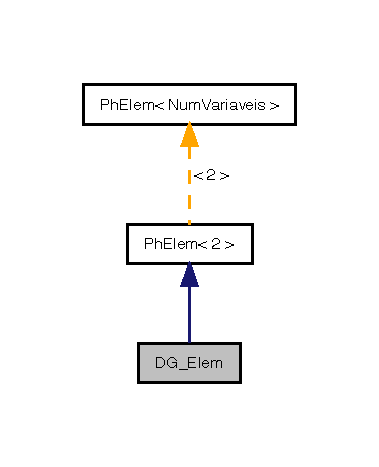
\includegraphics[width=182pt]{classDG__Elem__inherit__graph}
\end{center}
\end{figure}


Collaboration diagram for D\+G\+\_\+\+Elem\+:
\nopagebreak
\begin{figure}[H]
\begin{center}
\leavevmode
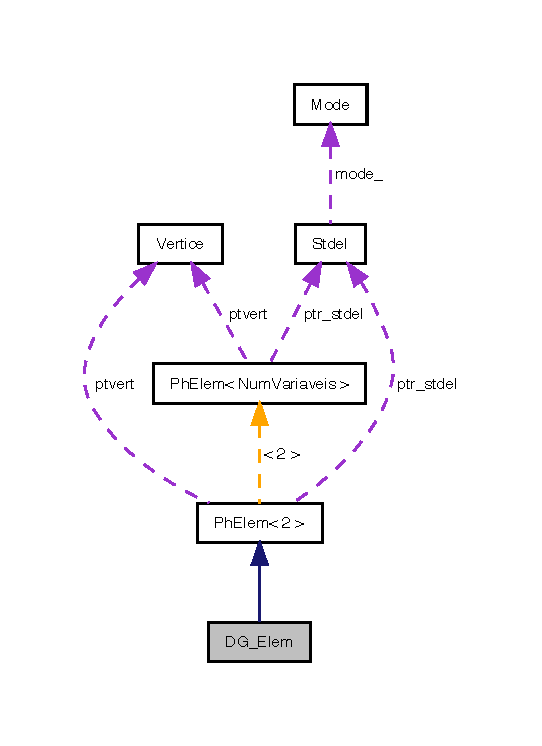
\includegraphics[width=260pt]{classDG__Elem__coll__graph}
\end{center}
\end{figure}
\subsection*{Public Member Functions}
\begin{DoxyCompactItemize}
\item 
\hyperlink{classDG__Elem_a9f40328ca740050c165ccffe11007d35}{D\+G\+\_\+\+Elem} ()
\item 
\hyperlink{classDG__Elem_af37ff3dd87674abfdd621f8cdba43975}{$\sim$\+D\+G\+\_\+\+Elem} ()
\item 
void \hyperlink{classDG__Elem_ac1ec1f962d6e1852f0adb01048c4c1f9}{inicia\+\_\+vetores} ()
\item 
void \hyperlink{classDG__Elem_a9f7165dbb388e11f16b4249383f71d0e}{set\+\_\+fontes} (double sw, double \hyperlink{DG__EI__Header_8h_a52e510ecdc11d9091099d94c3ba63e74}{sn})
\item 
double \hyperlink{classDG__Elem_acc7285f0df1d6a4544405169daf2853c}{show\+\_\+rho} ()
\item 
double \hyperlink{classDG__Elem_a01a49e07fd18a74e12eedf15cff7b8c7}{show\+\_\+\+Volume} ()
\item 
void \hyperlink{classDG__Elem_af61130ab38851fa2ade53f9e3f2418bc}{inicia\+\_\+funcoes\+\_\+na\+\_\+borda} (\hyperlink{structEDGE}{E\+D\+GE} $\ast$border)
\item 
void \hyperlink{classDG__Elem_af91d2d61c97fae30b8dfc6db67433094}{finaliza\+\_\+vetores} ()
\item 
void \hyperlink{classDG__Elem_a33d01f96cc0d00b6a1a1d4a817724b4c}{inicia\+\_\+tracos} (\hyperlink{structEDGE}{E\+D\+GE} $\ast$border)
\item 
void \hyperlink{classDG__Elem_ab5d89b8f7625699239440bfd0e8ec6e6}{echo\+\_\+traco} (F\+I\+LE $\ast$f\+\_\+eco=nullptr)
\item 
void \hyperlink{classDG__Elem_a70dbc366e1cdfb0b96fa9d640dcff689}{Atualizar\+\_\+valores} (F\+I\+LE $\ast$fout=N\+U\+LL)
\item 
void \hyperlink{classDG__Elem_a51393e54786059782e6a0502f00cdd50}{set\+\_\+permeabilidade} (const double, const double, const double)
\item 
void \hyperlink{classDG__Elem_a132e9ad800e701395b1e21d291040ff2}{set\+\_\+mass\+\_\+density} (double)
\item 
void \hyperlink{classDG__Elem_a5d8512886cb22395c92265f5eee6a940}{set\+\_\+porosidade} (double)
\item 
void \hyperlink{classDG__Elem_ab3de164caf40da7cc0b123928ad83cc9}{Volume\+Integrals\+\_\+\+U\+M\+F\+P\+A\+CK} (const double Dt, \hyperlink{classFluids}{Fluids} fls, int \&count, int $\ast$Ti, int $\ast$Tj, double $\ast$Tx, double $\ast$\hyperlink{ASPFunctions_8cpp_a57d673f8d6833fb7a7aced326df10ca9}{B}, double $\ast$=N\+U\+LL, double $\ast$=N\+U\+LL)
\item 
void \hyperlink{classDG__Elem_a166b7ad0ea852f703f65661c14b5c713}{Volume\+Integrals} (const double Dt, \hyperlink{classFluids}{Fluids} fls, Teuchos\+::\+R\+CP$<$ Epetra\+\_\+\+F\+E\+Crs\+Matrix $>$ A, Teuchos\+::\+R\+CP$<$ Epetra\+\_\+\+F\+E\+Vector $>$ R\+HS, double $\ast$=N\+U\+LL, double $\ast$=N\+U\+LL)
\item 
void \hyperlink{classDG__Elem_a84fab76e27b414367eb553f9d4841889}{Volume\+Tracos} (const double Dt, \hyperlink{classFluids}{Fluids} fls, double $\ast$=N\+U\+LL, double $\ast$=N\+U\+LL)
\item 
void \hyperlink{classDG__Elem_a2a2a90dfc3c456b66f7e1890d0f236f2}{Volume\+IntegralsT} (const double Dt\+\_\+new, const double Dt\+\_\+old, int \&count, int $\ast$Ti, int $\ast$Tj, double $\ast$Tx, double $\ast$\hyperlink{ASPFunctions_8cpp_a57d673f8d6833fb7a7aced326df10ca9}{B})
\item 
void \hyperlink{classDG__Elem_a64d352e6b9eeeeca73368a9ef92a94c2}{calcula\+\_\+tracos} (\hyperlink{classFluids}{Fluids} fls)
\item 
void \hyperlink{classDG__Elem_a3fc71dbfe141c0d42dc8ceff8f0ef8ce}{Volume\+Integrals\+\_\+\+IG} (\hyperlink{classFluids}{Fluids} fls, int \&count, int $\ast$Ti, int $\ast$Tj, double $\ast$Tx, double $\ast$\hyperlink{ASPFunctions_8cpp_a57d673f8d6833fb7a7aced326df10ca9}{B})
\item 
void \hyperlink{classDG__Elem_a699a198b44d02b1394229e623cd6632d}{perm\+\_\+val} (double K\mbox{[}3\mbox{]})
\item 
void \hyperlink{classDG__Elem_a4b5b26372a103e9f10c9d518419d4fd1}{Traco\+\_\+sn} (const int \&h, double $\ast$saida)
\item 
void \hyperlink{classDG__Elem_ab57a34a01c448785d8a887e51e7ab331}{Traco\+\_\+pw} (const int \&h, double $\ast$saida)
\item 
void \hyperlink{classDG__Elem_ae98efe920078bc5fd18eceee997d44a2}{Traco\+\_\+\+Kgrad\+\_\+pw} (const int \&h, double $\ast$$\ast$saida)
\item 
void \hyperlink{classDG__Elem_ad288d45acae59787b21a35b38fe47b10}{Traco\+\_\+\+Kgrad\+\_\+pc} (const int \&h, double $\ast$$\ast$saida)
\item 
void \hyperlink{classDG__Elem_ae64a1118040aad9dd3c18ac68b2d5d4f}{Traco\+\_\+\+Kgrad\+\_\+sn} (const int \&h, double $\ast$$\ast$saida)
\item 
void \hyperlink{classDG__Elem_aa97824992d60c2a7b5506e5d660dc7a1}{Traco\+\_\+phi} (const int \&lado, const int \&ivar, const int \&ind, double $\ast$saida)
\item 
void \hyperlink{classDG__Elem_a99f9e69fc0d6eacd683712bc456af5f7}{Traco\+\_\+phi\+\_\+1} (const int \&lado, const int \&ivar, const int \&\hyperlink{DG__EI__Header_8h_a1910d262855b71da353ed0d07a6c7823}{pos}, double $\ast$saida)
\item 
void \hyperlink{classDG__Elem_a8d090e18204cd99ed11ef8115a95c2e7}{Traco\+\_\+grad\+\_\+phi} (const int \&lado, const int \&ivar, const int \&ind, double $\ast$$\ast$saida)
\item 
void \hyperlink{classDG__Elem_a0109cc28854e31b5df555513e9fccfed}{Traco\+\_\+\+Kgrad\+\_\+phi\+\_\+n} (const int \&lado, const int \&ivar, const int \&ind, double $\ast$saida)
\item 
int \hyperlink{classPhElem_a5288b2eba55ffa37f1a9866a516f6886}{show\+\_\+\+Num\+Local\+Vars} ()
\item 
void \hyperlink{classPhElem_a9742fa2313cf25a24ae9c5602bd75ac0}{teste} ()
\item 
void \hyperlink{classPhElem_af2796c868709214bb9b151b47d7d471f}{set\+\_\+ptr\+\_\+stdel} (\hyperlink{classStdel}{Stdel} $\ast$pointer, \hyperlink{classStdel}{Stdel} $\ast$pointer1)
\item 
void \hyperlink{classPhElem_aaf841c14455a54e0f33e2c74bef979fd}{set\+\_\+ptr\+\_\+stdel} (\hyperlink{classStdel}{Stdel} $\ast$pointers\mbox{[}$\,$\mbox{]})
\item 
void \hyperlink{classPhElem_a78130ee8d7d6ecf59f231dbd436e9081}{set\+\_\+ptr\+\_\+stdel} (\hyperlink{classStdel}{Stdel} $\ast$pointer)
\item 
void \hyperlink{classPhElem_a52fdbcf2283aacd8fdf9672018d74e4a}{set\+\_\+ptr\+\_\+stdel\+\_\+var} (const int ind, \hyperlink{classStdel}{Stdel} $\ast$pointer)
\item 
void \hyperlink{classPhElem_a134cbfd28fc238a24156ab1c24fc31c0}{set\+\_\+\+Vert\+\_\+map} (const int \&n\+\_\+in, int ver\+\_\+temp\mbox{[}$\,$\mbox{]})
\item 
void \hyperlink{classPhElem_a8ed472a9e135b1e16b962c14df8f2225}{set\+\_\+ptvert} (const \hyperlink{structVertice}{Vertice} $\ast$pointer)
\item 
void \hyperlink{classPhElem_a8abc7be8120f4192de31e0cfb32ac968}{read\+\_\+vertices} (F\+I\+LE $\ast$, const int \&)
\item 
void \hyperlink{classPhElem_a03505c861fbcdb7cf8faec9fe5eea088}{set\+\_\+sgn} ()
\item 
int \hyperlink{classPhElem_ab271550e1373e11cb0b1f62d3e1ea428}{show\+\_\+sgn} (const int \&ia, const int \&i)
\item 
const int \hyperlink{classPhElem_a878851914f553298700437c5c8aef4dd}{show\+\_\+gbnmap} (int ivar, int modo) const
\item 
int \hyperlink{classPhElem_a69a5cfc5b3b7faa4ad5f584311406ce1}{show\+\_\+numv} ()
\item 
int \hyperlink{classPhElem_aca4ef303cd316714d116062e8f4d8ca5}{show\+\_\+nume} ()
\item 
int \hyperlink{classPhElem_afbe63a88e47733c8daec89a4c72b7da0}{show\+\_\+numf} ()
\item 
void \hyperlink{classPhElem_ae226a41912e8e7c76be365518b2a38e2}{set\+\_\+type} (const int \&num)
\item 
int \hyperlink{classPhElem_a4ea6c54e35eb46d331db770f992c4c4b}{type\+\_\+val} ()
\item 
void \hyperlink{classPhElem_a8d2c46990cba5a5459198d883b763eab}{print\+\_\+numeracao} (F\+I\+LE $\ast$fout, const int \&k)
\item 
void \hyperlink{classPhElem_ae7659320b2118608e38d192443bb2b8f}{print\+\_\+modes} (F\+I\+LE $\ast$fout, const int \&k) const
\item 
void \hyperlink{classPhElem_a46f2be4d83b5c7c2cc9c6699f1fe977c}{zera\+\_\+vetores} (const int \&k)
\item 
void \hyperlink{classPhElem_a55ef84501df0d4e8aec6d49846e21237}{zera\+\_\+bs} (const int \&k)
\item 
void \hyperlink{classPhElem_a5051606f1d1e914d52d3de8655195c9f}{make\+\_\+vector} (const int \&ia, double($\ast$f)(double, double, double))
\item 
void \hyperlink{classPhElem_ad5732b2fb83ab0d9a2de7678391f87c4}{make\+\_\+vector\+\_\+\+Elast2\+D\+\_\+dyn} (const double \hyperlink{DG__EI__Header_8h_a491bc358fce276972681cc0be8844bd7}{a}\mbox{[}$\,$\mbox{]})
\item 
void \hyperlink{classPhElem_a1223b3e50580a1a7959e5f3b665d0761}{make\+\_\+\+Kcomp\+\_\+\+Elast2D} (const double lambda, const double mu)
\item 
void \hyperlink{classPhElem_a1ce74128a48a212028f644a68ce8edc0}{make\+\_\+\+Kcomp\+\_\+\+Elast2\+D\+\_\+dyn} (const double lambda, const double mu, const double \hyperlink{DG__EI__Header_8h_a491bc358fce276972681cc0be8844bd7}{a}\mbox{[}$\,$\mbox{]})
\item 
void \hyperlink{classPhElem_ac59f1cbe0962524e3aa5eced9a4393f6}{make\+\_\+\+K\+\_\+\+Elast2D} (const double lambda, const double mu, double $\ast$$\ast$K)
\item 
void \hyperlink{classPhElem_a38499c9f62a291a880d72db646171cb5}{Vector\+Elast2D} (const int \&i, double sum\mbox{[}$\,$\mbox{]})
\item 
void \hyperlink{classPhElem_a4b130cb327652894d81b2c4e26b96f41}{Vector\+Elast2D} (double vector\mbox{[}$\,$\mbox{]})
\item 
void \hyperlink{classPhElem_ac3bc9b0559e940faa2404b1541d0c403}{P\+\_\+eval\+\_\+print\+\_\+\+Elast2D} (F\+I\+LE $\ast$fout, const double X\mbox{[}$\,$\mbox{]}, double lambda, double mu)
\item 
void \hyperlink{classPhElem_a467c1ae6065913d0ec9828c9d055539a}{P\+\_\+eval\+\_\+print\+\_\+\+Elast2\+D\+\_\+dyn} (F\+I\+LE $\ast$fout, const int \&prnflag, const double X\mbox{[}$\,$\mbox{]}, double lambda, double mu, const double \hyperlink{DG__EI__Header_8h_a491bc358fce276972681cc0be8844bd7}{a}\mbox{[}$\,$\mbox{]})
\item 
void \hyperlink{classPhElem_ae0418a5de14872e80fe4f9ffd9dd4fdd}{make\+\_\+\+K\+\_\+\+Imiscivel2F} (const double, const double, const double, const double, const double \mbox{[}$\,$\mbox{]}, double($\ast$)(double), double($\ast$)(double), double($\ast$)(double))
\item 
double \hyperlink{classPhElem_afdbe06fb407dc4c474b886ed219de195}{Kcomp} (const int \&i, const int \&j)
\item 
double \hyperlink{classPhElem_a3064c3377eb3f81d63f43969a3c958ee}{K\+\_\+\+Imisc2F} (const int \&i, const int \&j)
\item 
void \hyperlink{classPhElem_a5f08c96b39a608ac8500897535998d52}{make\+\_\+\+Vector\+\_\+\+Eq\+\_\+\+S1} (const double, const double, const double, const double, const double \mbox{[}3\mbox{]}, double($\ast$)(double))
\item 
int \hyperlink{classPhElem_a6b7f26c842b4f6b54782c6ddaa4fd6d6}{map} (const int \&var, const int \&no\+\_\+local)
\item 
void \hyperlink{classPhElem_aa53cc9dad058e9dbebfb971bdabe80fc}{mapa\+\_\+inverso} (const int \&ivar, const double X\mbox{[}$\,$\mbox{]})
\item 
void \hyperlink{classPhElem_acd85a3728b9566c086c1450a35e6231f}{P\+\_\+eval\+\_\+u} (const double X\mbox{[}$\,$\mbox{]})
\item 
void \hyperlink{classPhElem_aa648874799b8fa49fdccbcbc9b8de504}{P\+\_\+eval\+\_\+u} (const double X\mbox{[}$\,$\mbox{]}, const int \&ia)
\item 
void \hyperlink{classPhElem_a69032d622789084c4416981e2fceb80c}{P\+\_\+eval\+\_\+u\+\_\+p1} (const double X\mbox{[}$\,$\mbox{]}, const int \&ia)
\item 
void \hyperlink{classPhElem_ac5436d432516c731328134ac91b9a70b}{P\+\_\+eval\+\_\+print} (const double X\mbox{[}$\,$\mbox{]}, const int \&\hyperlink{classPhElem_a85d9a8342adf9e155a533edf165a6fe3}{numf}, F\+I\+LE $\ast$fout, double($\ast$)(double, double, double))
\item 
void \hyperlink{classPhElem_a1ae41c2b94f8faca55505d25e899f724}{P\+\_\+print} (const int \&\hyperlink{classPhElem_a85d9a8342adf9e155a533edf165a6fe3}{numf}, F\+I\+LE $\ast$file)
\item 
void \hyperlink{classPhElem_a115839e26aca8569ede2966db01926f1}{P\+\_\+eval\+\_\+vert} (const double X\mbox{[}$\,$\mbox{]}, double f\+\_\+vert\mbox{[}$\,$\mbox{]})
\item 
void \hyperlink{classPhElem_a638d823f66d1600cb948df872eb753c1}{P\+\_\+eval\+\_\+phys} (const int \&\hyperlink{classPhElem_a85d9a8342adf9e155a533edf165a6fe3}{numf}, double f0\mbox{[}$\,$\mbox{]})
\item 
void \hyperlink{classPhElem_afac13525ce0e8907ca74a7213aa72504}{Increment\+\_\+field} (const double X\mbox{[}$\,$\mbox{]}, const int \&\hyperlink{classPhElem_a85d9a8342adf9e155a533edf165a6fe3}{numf}, const double dt)
\item 
void \hyperlink{classPhElem_abc4450898733d818edaa51a7f0d2bb58}{compute\+\_\+\+JV} (const int \&ia)
\item 
void \hyperlink{classPhElem_a233fb1bc0c15cae815fef5d1dc8d9265}{print\+\_\+matrices} (F\+I\+LE $\ast$fout)
\item 
void \hyperlink{classPhElem_a6e4284fcb95240394293c1a576deb738}{Processar\+\_\+dados} (int \&NL, std\+::vector$<$ \hyperlink{structARESTA}{A\+R\+E\+S\+TA} $>$ \&aresta, int \&NF, std\+::vector$<$ \hyperlink{structFACE}{F\+A\+CE} $>$ \&face\+\_\+vec)
\item 
void \hyperlink{classPhElem_a76ba4a82c7f21f9a83808315903692fe}{check\+\_\+connectivity} (F\+I\+LE $\ast$fout, const int \&ia)
\item 
void \hyperlink{classPhElem_ac6ea940519c924130a4cb44bbab2a31d}{assign\+\_\+gbnmap} (const int \&ia, const int \&i, const int \&val)
\item 
void \hyperlink{classPhElem_a98449dc77f691781f54fc8798bea03a3}{inicia\+\_\+gbnmap} (int \&count)
\item 
void \hyperlink{classPhElem_a3ed7c7027c6fadd45f29eb7de33ee7fb}{inicia\+\_\+gbnmap} (const int \&ivar, int \&count)
\item 
void \hyperlink{classPhElem_a9b5610a7a12eddbc4a9f07429500a6da}{inicia\+\_\+gbtrbmap} (int \&count)
\item 
void \hyperlink{classPhElem_afba886f63bf7b67bd0a4164eae4dde5b}{set\+\_\+gbnmap} (const int \&ia, const int gbnmap\+\_\+temp\mbox{[}$\,$\mbox{]}, const int sgn\+\_\+temp\mbox{[}$\,$\mbox{]})
\item 
void \hyperlink{classPhElem_ae63196241e8f39617acb1984cb06910e}{set\+\_\+stgbtrbmap} (const int \&b, const int \&vmapM, const int \&vmapP)
\item 
int \hyperlink{classPhElem_a2addc4d79151aeac865e2255be3b417d}{show\+\_\+gbtrbmap} ()
\item 
int \hyperlink{classPhElem_a5f0e8811ea30343e51e4be9ff40d2b74}{show\+\_\+stgbtrbmapM} (const int \&\hyperlink{DG__EI__Header_8h_a491bc358fce276972681cc0be8844bd7}{a})
\item 
int \hyperlink{classPhElem_a3d9e8990f4442e3b17e1cce3c9af19e9}{show\+\_\+stgbtrbmapP} (const int \&\hyperlink{DG__EI__Header_8h_a491bc358fce276972681cc0be8844bd7}{a})
\item 
void \hyperlink{classPhElem_a298b653fae7c86dea6ad0eea09b7e621}{check\+\_\+gradiente} (F\+I\+LE $\ast$fout, const int \&ia)
\item 
\hyperlink{classStdel}{Stdel} $\ast$ \hyperlink{classPhElem_a227c31195c6832f8e36f8d507806bd54}{show\+\_\+ptr\+\_\+stdel} (const int \&n) const
\item 
void \hyperlink{classPhElem_a61311993fa273240a94044c599d52857}{Bound\+Cond} (const int \&face, int bflag\mbox{[}$\,$\mbox{]}, double bc\mbox{[}$\,$\mbox{]}, double($\ast$func)(double, double, double), const int \&nf, const int \&bndtype)
\item 
void \hyperlink{classPhElem_a857f4ffbef27f0ef054f59eceffbad27}{Neumann} (const int \&aresta, const int \&varn, const double rho1, const double mu1, const double rho2, const double mu2, const double gravidade\mbox{[}$\,$\mbox{]})
\item 
double \hyperlink{classPhElem_a27e7bc9ed0ea64d609d4d0b29baba468}{show\+\_\+u} (const int \&i)
\item 
double \hyperlink{classPhElem_a9d2b7b826289ccd180fdd4b45d0d7333}{show\+\_\+u} (const int \&, const int \&)
\item 
double \hyperlink{classPhElem_a0caf55d9fac7477102ee34373c67a024}{show\+\_\+b0} (const int \&i)
\item 
double \hyperlink{classPhElem_afb4171c67795f5614d9628d59f3bfaf7}{show\+\_\+b0} (const int \&, const int \&)
\item 
double \hyperlink{classPhElem_a0846ec2cbd31a24aea440c29a71d50ec}{show\+\_\+bs} (const int \&, const int \&)
\item 
double \hyperlink{classPhElem_a63b2f67b4f782432909cd7d32d188996}{show\+\_\+J} ()
\item 
void \hyperlink{classPhElem_ae538fb941f4cedc88e27dd28f2460bb5}{make\+\_\+\+Mass\+Matrices} ()
\item 
int \hyperlink{classPhElem_ace7e4ec0fa3ca3e829cd790375ab981e}{show\+\_\+\+Vert\+\_\+map} (int i)
\item 
int \hyperlink{classPhElem_ac6f5e03dd6e155037363dbd0ea2f401b}{show\+\_\+\+Aresta} (int i)
\item 
int \hyperlink{classPhElem_a916c6927d0964574d815a13dd80f1e30}{show\+\_\+\+Face} (int i)
\item 
int \hyperlink{classPhElem_a47dc705efd50a4484bf407bce4a5e010}{show\+\_\+sinal} (int i)
\item 
int \hyperlink{classPhElem_a13564919b6d9747f0e6b33f3e8aae31b}{show\+\_\+border\+\_\+num} (int i)
\item 
int \hyperlink{classPhElem_a7a476e9682accd03064f3e8bec39fb50}{show\+\_\+part\+\_\+num} ()
\item 
void \hyperlink{classPhElem_a24a705e62f179fa36c6886f8f0a3ef25}{set\+\_\+part\+\_\+num} (const int \&num=-\/1)
\item 
double \hyperlink{classPhElem_aa67e9fd1399ee905803999ef50581677}{Phi\+\_\+val} (const int \&var, const int \&ind, const int \&\hyperlink{DG__EI__Header_8h_a1910d262855b71da353ed0d07a6c7823}{pos})
\item 
void \hyperlink{classPhElem_aa5f168531640b2fb9ac82f85e5f8b11a}{projetar\+\_\+\+C0} (F\+I\+LE $\ast$file, double($\ast$func)(double, double, double), const int \&ivar)
\item 
void \hyperlink{classPhElem_a09b6787e5e42496ece86754bbb2ae59c}{transformacao\+\_\+direta} (double f\mbox{[}$\,$\mbox{]}, const int \&ivar)
\item 
void \hyperlink{classPhElem_a68e2ff863aa38d90933fc033e1fcec0e}{teste\+\_\+transformacao\+\_\+direta} (F\+I\+LE $\ast$fin, F\+I\+LE $\ast$fout, const int \&npoints, const double coord\mbox{[}$\,$\mbox{]})
\item 
void \hyperlink{classPhElem_aafd112d676dc3e16309e8ec8980f1c97}{set\+\_\+border\+\_\+tipo} (\hyperlink{structEDGE}{E\+D\+GE} $\ast$border, const int \&aresta, const int \&t)
\item 
void \hyperlink{classPhElem_a05b05802884ecd42ed42e46108a0d5b1}{set\+\_\+border\+\_\+num} (const int \&aresta, const int \&num)
\item 
void \hyperlink{classPhElem_a6f8258d7b66de04cd4d88f2c8af41541}{Imprimir\+\_\+valores} (F\+I\+LE $\ast$fileout, const int \&npoints, const double coord\mbox{[}$\,$\mbox{]})
\item 
void \hyperlink{classPhElem_a53eb1654e889d3fc893f50dcea12adcb}{printw\+G\+QJ} (F\+I\+LE $\ast$fileout)
\item 
void \hyperlink{classPhElem_a7dc16c86382b340e9d1c5983eb478cee}{Avancar\+\_\+u0} (const double X\mbox{[}$\,$\mbox{]}, const double relax=1.\+0)
\item 
void \hyperlink{classPhElem_aa3697427ea1b5024f52b98bcbcbb55f1}{Atualizar\+\_\+u0} (const double X\mbox{[}$\,$\mbox{]})
\item 
void \hyperlink{classPhElem_ac395c07742ced41887c4c12019454618}{Copia\+\_\+u0\+\_\+em\+\_\+} (double X\mbox{[}$\,$\mbox{]})
\item 
void \hyperlink{classPhElem_a3bc714a5f0ca21e0090e2d1747c0ec5a}{Copia\+\_\+u0\+\_\+em\+\_\+} (Teuchos\+::\+R\+CP$<$ Epetra\+\_\+\+Vector $>$ X)
\item 
void \hyperlink{classPhElem_a9ea744b94e057733c1d396d9f46ddcce}{Comparar\+\_\+u0} (const double X\mbox{[}$\,$\mbox{]})
\item 
void \hyperlink{classPhElem_ab6765ea1fa41b3a2d565d86872d6e7e6}{Salvar\+\_\+u0} ()
\item 
void \hyperlink{classPhElem_a7094a0e8767868c583cc948e56214a9d}{Restaurar\+\_\+u0} ()
\item 
void \hyperlink{classPhElem_a11a736e86c5b40e5b0a4c84754f2b066}{escrever\+\_\+restart} (F\+I\+LE $\ast$fout)
\item 
void \hyperlink{classPhElem_a0209eb7e6db7b0b541b51c46269ee9b6}{ler\+\_\+restart} (F\+I\+LE $\ast$fin)
\item 
void \hyperlink{classPhElem_ad0a2992e6d206b6a351da8847a9dd69a}{ler\+\_\+restart\+\_\+buffer} (F\+I\+LE $\ast$fin, double $\ast$buff, int \&count)
\item 
void \hyperlink{classPhElem_abe273d496e748985021a8f67ef598c0d}{restart\+\_\+element} (double $\ast$buff, int \&count)
\item 
void \hyperlink{classPhElem_adc3411d8b3a88f04004b6d48e64e9334}{teste\+\_\+gradiente} ()
\item 
int \hyperlink{classPhElem_a35508e257e1675a912954f83cb4b6a3e}{get\+\_\+trace\+\_\+border\+\_\+map} (const int \&aresta)
\item 
void \hyperlink{classPhElem_ad8d5bac3d1866cfe20daec73fc405b05}{gbnmap\+\_\+vertices} (std\+::vector$<$ std\+::vector$<$ int $>$$>$ gbn)
\item 
void \hyperlink{classPhElem_a75f80b321d33ea208ae2d35af1b8c4df}{gbnmap\+\_\+vertices} (int $\ast$gbn, const int \&ivar)
\item 
void \hyperlink{classPhElem_ad355231f4e2807541c62212647c44b3e}{gbnmap\+\_\+faces} (const int face\+\_\+vec\mbox{[}$\,$\mbox{]}, const int \&ivar)
\item 
void \hyperlink{classPhElem_a19299ae55f9faef322a1d21d7e9b2a88}{gbnmap\+\_\+aresta} (const int \&aresta, const int \&\hyperlink{classPhElem_a4034b9b2a458d1277ca74e4e8a49627e}{sinal}, const int \&ivar, const int \&count, int \&inc)
\item 
void \hyperlink{classPhElem_af545eccd164b2fc7ca104afff13a50c6}{gbnmap\+\_\+arestas} (const int aresta\+\_\+vec\mbox{[}$\,$\mbox{]}, const int \&ivar)
\item 
void \hyperlink{classPhElem_ae6f35113c182e2678646552e6c4a752c}{gbnmap\+\_\+interior} (const int \&ivar, int \&count)
\item 
void \hyperlink{classPhElem_a4da3f8bc24014789f4685c9a611a11dc}{anexa\+\_\+gbnmap} (const int \&ivar, vector$<$ int $>$ \&)
\item 
void \hyperlink{classPhElem_a993d5f1b66f6d99ffb95adc9ff882e80}{vetor\+\_\+superficie} (const int \&num\+\_\+local, double \&area, double normal\mbox{[}3\mbox{]})
\end{DoxyCompactItemize}
\subsection*{Protected Attributes}
\begin{DoxyCompactItemize}
\item 
\hyperlink{classStdel}{Stdel} $\ast$ \hyperlink{classPhElem_a7b4509b90bcf92be76cd8fdb76d7385b}{ptr\+\_\+stdel} \mbox{[}Num\+Variaveis\mbox{]}
\item 
int \hyperlink{classPhElem_a1ed1b45136a718afef64c846fb905546}{type}
\item 
const \hyperlink{structVertice}{Vertice} $\ast$ \hyperlink{classPhElem_a92acc9f8f36991ce851df5e462425d3c}{ptvert}
\item 
int \hyperlink{classPhElem_a2ec71d768628a94d7fbe74be08a08ea9}{Num\+Local\+Vars}
\item 
int \hyperlink{classPhElem_af3ea3f4193f7d65855c3fabead6f2545}{ndim}
\begin{DoxyCompactList}\small\item\em Spatial dimension. \end{DoxyCompactList}\item 
int \hyperlink{classPhElem_a67ed36925b04bf0f2d177c8d31737526}{numv}
\begin{DoxyCompactList}\small\item\em Number of vertices. \end{DoxyCompactList}\item 
int \hyperlink{classPhElem_a1c0c7833feba84d4ed83d172244ca3e1}{nume}
\begin{DoxyCompactList}\small\item\em Number of edges. \end{DoxyCompactList}\item 
int \hyperlink{classPhElem_a85d9a8342adf9e155a533edf165a6fe3}{numf}
\begin{DoxyCompactList}\small\item\em Number of faces. \end{DoxyCompactList}\item 
int \hyperlink{classPhElem_ad24d6fbe02539875405dd4a6cf094284}{numborders}
\begin{DoxyCompactList}\small\item\em Number of borders in the element. \end{DoxyCompactList}\item 
int \hyperlink{classPhElem_a8e65fa4998d28b9b8db9b6fcf8999d20}{numn} \mbox{[}Num\+Variaveis\mbox{]}
\item 
int \hyperlink{classPhElem_ad95c9f8ee7a993ccc7f9cdd08dddf5f6}{numb} \mbox{[}Num\+Variaveis\mbox{]}
\item 
int \hyperlink{classPhElem_a07f19f862b13cc9c5f80271b03a5a023}{Vert\+\_\+map} \mbox{[}8\mbox{]}
\item 
int \hyperlink{classPhElem_a27a4f856d62b68758e4c03c09b4c37f8}{aresta\+\_\+map} \mbox{[}12\mbox{]}
\item 
int \hyperlink{classPhElem_a300b484c07390b9016d9ed97980d76b3}{face\+\_\+map} \mbox{[}6\mbox{]}
\item 
int \hyperlink{classPhElem_ad153ce0aef191aac0f28f2addd213c71}{border\+\_\+num} \mbox{[}12\mbox{]}
\item 
int \hyperlink{classPhElem_a4034b9b2a458d1277ca74e4e8a49627e}{sinal} \mbox{[}12\mbox{]}
\begin{DoxyCompactList}\small\item\em sinal refers to the borders \end{DoxyCompactList}\item 
int \hyperlink{classPhElem_a141616ccadb4a17328626befc4330932}{part\+\_\+num}
\begin{DoxyCompactList}\small\item\em numero da particao a qual pertence \end{DoxyCompactList}\item 
int \hyperlink{classPhElem_ab27e9040a72ec923a90cffb25f5b0c15}{gbnmap} \mbox{[}Num\+Variaveis\mbox{]}\mbox{[}\hyperlink{MyOptions_8h_a2f91e7a0b4bf68a62a0f3d38904dea2c}{M\+A\+X\+NN}\mbox{]}
\begin{DoxyCompactList}\small\item\em mapping from local to global nodes (or modes) \end{DoxyCompactList}\item 
int \hyperlink{classPhElem_a5bb9ccd4ccebf12ff0937d807c443caf}{sgn} \mbox{[}Num\+Variaveis\mbox{]}\mbox{[}\hyperlink{MyOptions_8h_a2f91e7a0b4bf68a62a0f3d38904dea2c}{M\+A\+X\+NN}\mbox{]}
\begin{DoxyCompactList}\small\item\em sign of the local mode (or mode) \end{DoxyCompactList}\item 
double \hyperlink{classPhElem_a27acf6bc6ac9eaf94a7cce52522b3b92}{J}
\begin{DoxyCompactList}\small\item\em Jacobian from the physical to the standard element. \end{DoxyCompactList}\item 
double $\ast$ \hyperlink{classPhElem_a569278e8b30ca90d0e6f920b5bba7dd5}{JV}
\begin{DoxyCompactList}\small\item\em Ponteiro para matriz do Jacobiano nos pontos gaussianos;. \end{DoxyCompactList}\item 
double $\ast$ \hyperlink{classPhElem_aeaebffae27dd713bbc06ad07b7b727a3}{b0} \mbox{[}Num\+Variaveis\mbox{]}
\begin{DoxyCompactList}\small\item\em \mbox{[}M\+A\+X\+M\+O\+D\+E\+S$\ast$\+M\+A\+X\+N\+F\+I\+E\+L\+DS\mbox{]}; vector of body forces \end{DoxyCompactList}\item 
double $\ast$ \hyperlink{classPhElem_a42b747116ec9223cdebbc424e27f4089}{bs} \mbox{[}Num\+Variaveis\mbox{]}
\begin{DoxyCompactList}\small\item\em vector of force boundary conditions \end{DoxyCompactList}\item 
double $\ast$ \hyperlink{classPhElem_a560dc47ac8a684d84b05851ce52e044b}{u0} \mbox{[}Num\+Variaveis\mbox{]}
\begin{DoxyCompactList}\small\item\em vector with the coefficients of each mode \end{DoxyCompactList}\item 
double $\ast$ \hyperlink{classPhElem_a98781f3744597bad01eff75b31734d4b}{usave} \mbox{[}Num\+Variaveis\mbox{]}
\item 
int \hyperlink{classPhElem_a8188f64662092eb065a85d49f3ae6649}{gbtrbmap}
\begin{DoxyCompactList}\small\item\em Beginning index on the global array where the local border Gauss quadrature points (traces) are mapped; this map facilitates the use of mpi for paralell calculations over element borders. \end{DoxyCompactList}\item 
int $\ast$ \hyperlink{classPhElem_aebcf76eedfef93aef801fa3cab9c2708}{stgbtrbmapM}
\begin{DoxyCompactList}\small\item\em Array containing the start point in the global trace array of the internal trace of the border. \end{DoxyCompactList}\item 
int $\ast$ \hyperlink{classPhElem_a6b38afded290e7a4cfb4a215a7ebec4e}{stgbtrbmapP}
\begin{DoxyCompactList}\small\item\em Array containing the start point in the global trace array of the external trace of the border. \end{DoxyCompactList}\item 
int \hyperlink{classPhElem_a65f545dc1bf0d90240419934eb711a9d}{vetores\+\_\+iniciados}
\end{DoxyCompactItemize}
\subsection*{Private Attributes}
\begin{DoxyCompactItemize}
\item 
double $\ast$ \hyperlink{classDG__Elem_ac036921322e2a7d3648723ae77592af5}{sna}
\item 
double $\ast$ \hyperlink{classDG__Elem_afc53954789d7ec74b2cf2eb2be590d16}{pwa}
\begin{DoxyCompactList}\small\item\em ponteiros para os valores nos pontos de Gauss da saturacao e pressao atuais \end{DoxyCompactList}\item 
double \hyperlink{classDG__Elem_a56be853c8e67f9ee71f6b07aa99b3a58}{rho}
\begin{DoxyCompactList}\small\item\em densidade de massa ou porosidade \end{DoxyCompactList}\item 
double \hyperlink{classDG__Elem_a0bb64698c7f238bf48da2d584965fcd0}{porosidade}
\item 
double \hyperlink{classDG__Elem_a4b1a31424c3c115bc5bb964c3b72be66}{perm} \mbox{[}3\mbox{]}
\begin{DoxyCompactList}\small\item\em permeabilidades nas 3 direcoes \end{DoxyCompactList}\item 
double \hyperlink{classDG__Elem_a769560386db7e7c3b64d440ed84156be}{qn}
\item 
double \hyperlink{classDG__Elem_a89d2130d5e677207cb6c962dc90f79b3}{qw}
\item 
double \hyperlink{classDG__Elem_aeb8874934ea534afbee1017456e54051}{Volume}
\begin{DoxyCompactList}\small\item\em Volume do elemento ( = area do elemento para elementos bidimensionais e comprimento para elem. 1D. \end{DoxyCompactList}\item 
double $\ast$ \hyperlink{classDG__Elem_a21966ef258f170053e616e17082516c8}{Jb}
\begin{DoxyCompactList}\small\item\em Jacobiano nos pontos de Gauss sobre as bordas; usado na integração sobre bordas. \end{DoxyCompactList}\item 
double $\ast$$\ast$ \hyperlink{classDG__Elem_a53a6e2f1c4d46714b67f131f44902fc3}{Mass\+\_\+sn}
\item 
double $\ast$$\ast$ \hyperlink{classDG__Elem_a57d06772c710267516e58be078a6635b}{Trsn}
\item 
double $\ast$$\ast$ \hyperlink{classDG__Elem_a77316e95196e96ce7b612334075c8307}{Trpw}
\item 
double $\ast$$\ast$$\ast$ \hyperlink{classDG__Elem_a32939229d5c3e35ef503c432975949cc}{Laplaciano\+Phi}
\item 
double $\ast$$\ast$$\ast$ \hyperlink{classDG__Elem_aa71a1b860606c8560d0ef2a981580340}{Tr\+Kgrad\+\_\+sn}
\item 
double $\ast$$\ast$$\ast$ \hyperlink{classDG__Elem_a9c510976b9964cc09f695b5c1becbc2e}{Tr\+Kgrad\+\_\+pw}
\item 
double $\ast$$\ast$$\ast$ \hyperlink{classDG__Elem_a57dac9aed0b175230089be51335e2dfa}{Tr\+Kgrad\+\_\+pc}
\item 
double $\ast$$\ast$$\ast$$\ast$ \hyperlink{classDG__Elem_ae1432d30cbd7b063fc859a65362ee8bf}{Tr\+Phi}
\item 
double $\ast$$\ast$$\ast$$\ast$ \hyperlink{classDG__Elem_a89a6e65d3cca9d70aff0af308e1c4828}{Grad\+Phi}
\item 
double $\ast$$\ast$$\ast$$\ast$ \hyperlink{classDG__Elem_a2703c18a4eb102761f135b01958110c6}{Tr\+Kgrad\+Phi\+\_\+n}
\item 
double $\ast$$\ast$$\ast$$\ast$$\ast$ \hyperlink{classDG__Elem_acb3ed0d11e27ceae8f0f7c33496aa7e8}{Tr\+Grad\+Phi}
\item 
double $\ast$ \hyperlink{classDG__Elem_a79caff690ab51cd79dabbb5fd110d111}{Phi\+Array}
\end{DoxyCompactItemize}


\subsection{Detailed Description}


Definition at line 19 of file D\+G\+\_\+\+Elem.\+hpp.



\subsection{Constructor \& Destructor Documentation}
\mbox{\Hypertarget{classDG__Elem_a9f40328ca740050c165ccffe11007d35}\label{classDG__Elem_a9f40328ca740050c165ccffe11007d35}} 
\index{D\+G\+\_\+\+Elem@{D\+G\+\_\+\+Elem}!D\+G\+\_\+\+Elem@{D\+G\+\_\+\+Elem}}
\index{D\+G\+\_\+\+Elem@{D\+G\+\_\+\+Elem}!D\+G\+\_\+\+Elem@{D\+G\+\_\+\+Elem}}
\subsubsection{\texorpdfstring{D\+G\+\_\+\+Elem()}{DG\_Elem()}}
{\footnotesize\ttfamily D\+G\+\_\+\+Elem\+::\+D\+G\+\_\+\+Elem (\begin{DoxyParamCaption}{ }\end{DoxyParamCaption})\hspace{0.3cm}{\ttfamily [inline]}}



Definition at line 23 of file D\+G\+\_\+\+Elem.\+hpp.



References rho, and Ph\+Elem$<$ 2 $>$\+::vetores\+\_\+iniciados.

\mbox{\Hypertarget{classDG__Elem_af37ff3dd87674abfdd621f8cdba43975}\label{classDG__Elem_af37ff3dd87674abfdd621f8cdba43975}} 
\index{D\+G\+\_\+\+Elem@{D\+G\+\_\+\+Elem}!````~D\+G\+\_\+\+Elem@{$\sim$\+D\+G\+\_\+\+Elem}}
\index{````~D\+G\+\_\+\+Elem@{$\sim$\+D\+G\+\_\+\+Elem}!D\+G\+\_\+\+Elem@{D\+G\+\_\+\+Elem}}
\subsubsection{\texorpdfstring{$\sim$\+D\+G\+\_\+\+Elem()}{~DG\_Elem()}}
{\footnotesize\ttfamily D\+G\+\_\+\+Elem\+::$\sim$\+D\+G\+\_\+\+Elem (\begin{DoxyParamCaption}{ }\end{DoxyParamCaption})\hspace{0.3cm}{\ttfamily [inline]}}



Definition at line 24 of file D\+G\+\_\+\+Elem.\+hpp.



References inicia\+\_\+vetores().

Here is the call graph for this function\+:
\nopagebreak
\begin{figure}[H]
\begin{center}
\leavevmode
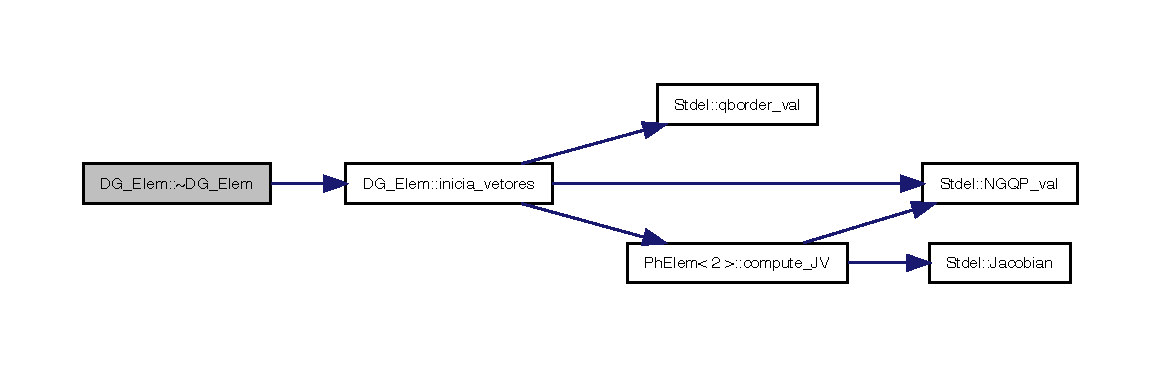
\includegraphics[width=350pt]{classDG__Elem_af37ff3dd87674abfdd621f8cdba43975_cgraph}
\end{center}
\end{figure}


\subsection{Member Function Documentation}
\mbox{\Hypertarget{classPhElem_a4da3f8bc24014789f4685c9a611a11dc}\label{classPhElem_a4da3f8bc24014789f4685c9a611a11dc}} 
\index{D\+G\+\_\+\+Elem@{D\+G\+\_\+\+Elem}!anexa\+\_\+gbnmap@{anexa\+\_\+gbnmap}}
\index{anexa\+\_\+gbnmap@{anexa\+\_\+gbnmap}!D\+G\+\_\+\+Elem@{D\+G\+\_\+\+Elem}}
\subsubsection{\texorpdfstring{anexa\+\_\+gbnmap()}{anexa\_gbnmap()}}
{\footnotesize\ttfamily void \hyperlink{classPhElem}{Ph\+Elem}$<$ Num\+Variaveis $>$\+::anexa\+\_\+gbnmap (\begin{DoxyParamCaption}\item[{const int \&}]{ivar,  }\item[{vector$<$ int $>$ \&}]{list }\end{DoxyParamCaption})\hspace{0.3cm}{\ttfamily [inherited]}}



Definition at line 308 of file Ph\+Elem.\+hpp.



References Ph\+Elem$<$ Num\+Variaveis $>$\+::gbnmap, and Ph\+Elem$<$ Num\+Variaveis $>$\+::numn.

\mbox{\Hypertarget{classPhElem_ac6ea940519c924130a4cb44bbab2a31d}\label{classPhElem_ac6ea940519c924130a4cb44bbab2a31d}} 
\index{D\+G\+\_\+\+Elem@{D\+G\+\_\+\+Elem}!assign\+\_\+gbnmap@{assign\+\_\+gbnmap}}
\index{assign\+\_\+gbnmap@{assign\+\_\+gbnmap}!D\+G\+\_\+\+Elem@{D\+G\+\_\+\+Elem}}
\subsubsection{\texorpdfstring{assign\+\_\+gbnmap()}{assign\_gbnmap()}}
{\footnotesize\ttfamily void \hyperlink{classPhElem}{Ph\+Elem}$<$ Num\+Variaveis $>$\+::assign\+\_\+gbnmap (\begin{DoxyParamCaption}\item[{const int \&}]{ia,  }\item[{const int \&}]{i,  }\item[{const int \&}]{val }\end{DoxyParamCaption})\hspace{0.3cm}{\ttfamily [inherited]}}



Definition at line 830 of file Ph\+Elem.\+hpp.



References Ph\+Elem$<$ Num\+Variaveis $>$\+::gbnmap.

\mbox{\Hypertarget{classPhElem_aa3697427ea1b5024f52b98bcbcbb55f1}\label{classPhElem_aa3697427ea1b5024f52b98bcbcbb55f1}} 
\index{D\+G\+\_\+\+Elem@{D\+G\+\_\+\+Elem}!Atualizar\+\_\+u0@{Atualizar\+\_\+u0}}
\index{Atualizar\+\_\+u0@{Atualizar\+\_\+u0}!D\+G\+\_\+\+Elem@{D\+G\+\_\+\+Elem}}
\subsubsection{\texorpdfstring{Atualizar\+\_\+u0()}{Atualizar\_u0()}}
{\footnotesize\ttfamily void \hyperlink{classPhElem}{Ph\+Elem}$<$ Num\+Variaveis $>$\+::Atualizar\+\_\+u0 (\begin{DoxyParamCaption}\item[{const double}]{X\mbox{[}$\,$\mbox{]} }\end{DoxyParamCaption})\hspace{0.3cm}{\ttfamily [inherited]}}



Definition at line 377 of file Ph\+Elem.\+hpp.



References Ph\+Elem$<$ Num\+Variaveis $>$\+::gbnmap, Ph\+Elem$<$ Num\+Variaveis $>$\+::numn, and Ph\+Elem$<$ Num\+Variaveis $>$\+::u0.

\mbox{\Hypertarget{classDG__Elem_a70dbc366e1cdfb0b96fa9d640dcff689}\label{classDG__Elem_a70dbc366e1cdfb0b96fa9d640dcff689}} 
\index{D\+G\+\_\+\+Elem@{D\+G\+\_\+\+Elem}!Atualizar\+\_\+valores@{Atualizar\+\_\+valores}}
\index{Atualizar\+\_\+valores@{Atualizar\+\_\+valores}!D\+G\+\_\+\+Elem@{D\+G\+\_\+\+Elem}}
\subsubsection{\texorpdfstring{Atualizar\+\_\+valores()}{Atualizar\_valores()}}
{\footnotesize\ttfamily void D\+G\+\_\+\+Elem\+::\+Atualizar\+\_\+valores (\begin{DoxyParamCaption}\item[{F\+I\+LE $\ast$}]{fout = {\ttfamily NULL} }\end{DoxyParamCaption})}



Definition at line 15 of file D\+G\+\_\+\+Elem.\+cpp.



References Stdel\+::eval\+G\+Q(), pres, Stdel\+::print\+G\+Qtofile(), Ph\+Elem$<$ 2 $>$\+::ptr\+\_\+stdel, Ph\+Elem$<$ 2 $>$\+::ptvert, pwa, sat, sna, Ph\+Elem$<$ 2 $>$\+::u0, and Ph\+Elem$<$ 2 $>$\+::\+Vert\+\_\+map.



Referenced by D\+G\+\_\+\+Prob\+::\+D\+G\+\_\+initial\+\_\+conditions(), and show\+\_\+\+Volume().

Here is the call graph for this function\+:
\nopagebreak
\begin{figure}[H]
\begin{center}
\leavevmode
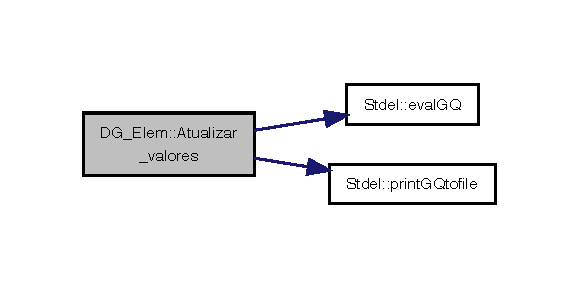
\includegraphics[width=278pt]{classDG__Elem_a70dbc366e1cdfb0b96fa9d640dcff689_cgraph}
\end{center}
\end{figure}
Here is the caller graph for this function\+:
\nopagebreak
\begin{figure}[H]
\begin{center}
\leavevmode
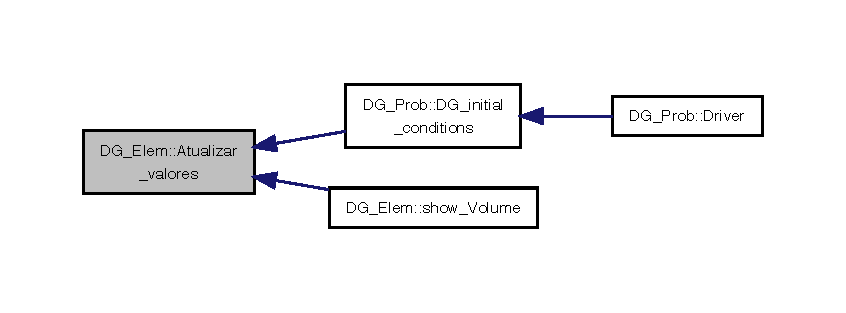
\includegraphics[width=350pt]{classDG__Elem_a70dbc366e1cdfb0b96fa9d640dcff689_icgraph}
\end{center}
\end{figure}
\mbox{\Hypertarget{classPhElem_a7dc16c86382b340e9d1c5983eb478cee}\label{classPhElem_a7dc16c86382b340e9d1c5983eb478cee}} 
\index{D\+G\+\_\+\+Elem@{D\+G\+\_\+\+Elem}!Avancar\+\_\+u0@{Avancar\+\_\+u0}}
\index{Avancar\+\_\+u0@{Avancar\+\_\+u0}!D\+G\+\_\+\+Elem@{D\+G\+\_\+\+Elem}}
\subsubsection{\texorpdfstring{Avancar\+\_\+u0()}{Avancar\_u0()}}
{\footnotesize\ttfamily void \hyperlink{classPhElem}{Ph\+Elem}$<$ Num\+Variaveis $>$\+::Avancar\+\_\+u0 (\begin{DoxyParamCaption}\item[{const double}]{X\mbox{[}$\,$\mbox{]},  }\item[{const double}]{relax = {\ttfamily 1.0} }\end{DoxyParamCaption})\hspace{0.3cm}{\ttfamily [inherited]}}



Definition at line 342 of file Ph\+Elem.\+hpp.



References Ph\+Elem$<$ Num\+Variaveis $>$\+::gbnmap, Ph\+Elem$<$ Num\+Variaveis $>$\+::numn, and Ph\+Elem$<$ Num\+Variaveis $>$\+::u0.

\mbox{\Hypertarget{classPhElem_a61311993fa273240a94044c599d52857}\label{classPhElem_a61311993fa273240a94044c599d52857}} 
\index{D\+G\+\_\+\+Elem@{D\+G\+\_\+\+Elem}!Bound\+Cond@{Bound\+Cond}}
\index{Bound\+Cond@{Bound\+Cond}!D\+G\+\_\+\+Elem@{D\+G\+\_\+\+Elem}}
\subsubsection{\texorpdfstring{Bound\+Cond()}{BoundCond()}}
{\footnotesize\ttfamily void \hyperlink{classPhElem}{Ph\+Elem}$<$ Num\+Variaveis $>$\+::Bound\+Cond (\begin{DoxyParamCaption}\item[{const int \&}]{face,  }\item[{int}]{bflag\mbox{[}$\,$\mbox{]},  }\item[{double}]{bc\mbox{[}$\,$\mbox{]},  }\item[{double($\ast$)(double, double, double)}]{func,  }\item[{const int \&}]{nf,  }\item[{const int \&}]{bndtype }\end{DoxyParamCaption})\hspace{0.3cm}{\ttfamily [inherited]}}

\mbox{\Hypertarget{classDG__Elem_a64d352e6b9eeeeca73368a9ef92a94c2}\label{classDG__Elem_a64d352e6b9eeeeca73368a9ef92a94c2}} 
\index{D\+G\+\_\+\+Elem@{D\+G\+\_\+\+Elem}!calcula\+\_\+tracos@{calcula\+\_\+tracos}}
\index{calcula\+\_\+tracos@{calcula\+\_\+tracos}!D\+G\+\_\+\+Elem@{D\+G\+\_\+\+Elem}}
\subsubsection{\texorpdfstring{calcula\+\_\+tracos()}{calcula\_tracos()}}
{\footnotesize\ttfamily void D\+G\+\_\+\+Elem\+::calcula\+\_\+tracos (\begin{DoxyParamCaption}\item[{\hyperlink{classFluids}{Fluids}}]{fls }\end{DoxyParamCaption})}



Definition at line 222 of file D\+G\+\_\+\+Elem.\+cpp.



References aux, aux1, Fluids\+::dpc(), Ph\+Elem$<$ 2 $>$\+::ndim, Ph\+Elem$<$ 2 $>$\+::numborders, Ph\+Elem$<$ 2 $>$\+::numn, perm, pos, pres, Ph\+Elem$<$ 2 $>$\+::ptr\+\_\+stdel, Stdel\+::qborder\+\_\+val(), sat, Tr\+Grad\+Phi, Tr\+Kgrad\+\_\+pc, Tr\+Kgrad\+\_\+pw, Tr\+Kgrad\+\_\+sn, Tr\+Phi, Trpw, Trsn, and Ph\+Elem$<$ 2 $>$\+::u0.



Referenced by show\+\_\+\+Volume().

Here is the call graph for this function\+:
\nopagebreak
\begin{figure}[H]
\begin{center}
\leavevmode
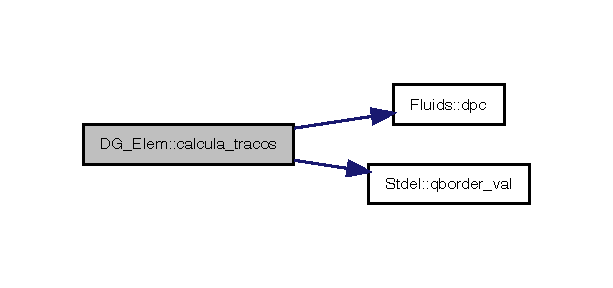
\includegraphics[width=294pt]{classDG__Elem_a64d352e6b9eeeeca73368a9ef92a94c2_cgraph}
\end{center}
\end{figure}
Here is the caller graph for this function\+:
\nopagebreak
\begin{figure}[H]
\begin{center}
\leavevmode
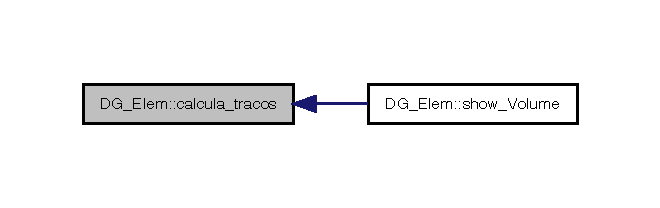
\includegraphics[width=317pt]{classDG__Elem_a64d352e6b9eeeeca73368a9ef92a94c2_icgraph}
\end{center}
\end{figure}
\mbox{\Hypertarget{classPhElem_a76ba4a82c7f21f9a83808315903692fe}\label{classPhElem_a76ba4a82c7f21f9a83808315903692fe}} 
\index{D\+G\+\_\+\+Elem@{D\+G\+\_\+\+Elem}!check\+\_\+connectivity@{check\+\_\+connectivity}}
\index{check\+\_\+connectivity@{check\+\_\+connectivity}!D\+G\+\_\+\+Elem@{D\+G\+\_\+\+Elem}}
\subsubsection{\texorpdfstring{check\+\_\+connectivity()}{check\_connectivity()}}
{\footnotesize\ttfamily void \hyperlink{classPhElem}{Ph\+Elem}$<$ Num\+Variaveis $>$\+::check\+\_\+connectivity (\begin{DoxyParamCaption}\item[{F\+I\+LE $\ast$}]{fout,  }\item[{const int \&}]{ia }\end{DoxyParamCaption})\hspace{0.3cm}{\ttfamily [inherited]}}



Definition at line 800 of file Ph\+Elem.\+hpp.



References Ph\+Elem$<$ Num\+Variaveis $>$\+::gbnmap, Ph\+Elem$<$ Num\+Variaveis $>$\+::numb, Ph\+Elem$<$ Num\+Variaveis $>$\+::ptr\+\_\+stdel, and Stdel\+::show\+\_\+ind().

\mbox{\Hypertarget{classPhElem_a298b653fae7c86dea6ad0eea09b7e621}\label{classPhElem_a298b653fae7c86dea6ad0eea09b7e621}} 
\index{D\+G\+\_\+\+Elem@{D\+G\+\_\+\+Elem}!check\+\_\+gradiente@{check\+\_\+gradiente}}
\index{check\+\_\+gradiente@{check\+\_\+gradiente}!D\+G\+\_\+\+Elem@{D\+G\+\_\+\+Elem}}
\subsubsection{\texorpdfstring{check\+\_\+gradiente()}{check\_gradiente()}}
{\footnotesize\ttfamily void \hyperlink{classPhElem}{Ph\+Elem}$<$ Num\+Variaveis $>$\+::check\+\_\+gradiente (\begin{DoxyParamCaption}\item[{F\+I\+LE $\ast$}]{fout,  }\item[{const int \&}]{ia }\end{DoxyParamCaption})\hspace{0.3cm}{\ttfamily [inherited]}}



Definition at line 811 of file Ph\+Elem.\+hpp.



References Stdel\+::eval\+G\+Q(), Stdel\+::\+Gradiente(), Ph\+Elem$<$ Num\+Variaveis $>$\+::ndim, Stdel\+::\+N\+G\+Q\+P\+\_\+val(), Ph\+Elem$<$ Num\+Variaveis $>$\+::ptr\+\_\+stdel, Ph\+Elem$<$ Num\+Variaveis $>$\+::ptvert, sn, Ph\+Elem$<$ Num\+Variaveis $>$\+::u0, and Ph\+Elem$<$ Num\+Variaveis $>$\+::\+Vert\+\_\+map.

\mbox{\Hypertarget{classPhElem_a9ea744b94e057733c1d396d9f46ddcce}\label{classPhElem_a9ea744b94e057733c1d396d9f46ddcce}} 
\index{D\+G\+\_\+\+Elem@{D\+G\+\_\+\+Elem}!Comparar\+\_\+u0@{Comparar\+\_\+u0}}
\index{Comparar\+\_\+u0@{Comparar\+\_\+u0}!D\+G\+\_\+\+Elem@{D\+G\+\_\+\+Elem}}
\subsubsection{\texorpdfstring{Comparar\+\_\+u0()}{Comparar\_u0()}}
{\footnotesize\ttfamily void \hyperlink{classPhElem}{Ph\+Elem}$<$ Num\+Variaveis $>$\+::Comparar\+\_\+u0 (\begin{DoxyParamCaption}\item[{const double}]{X\mbox{[}$\,$\mbox{]} }\end{DoxyParamCaption})\hspace{0.3cm}{\ttfamily [inherited]}}



Definition at line 358 of file Ph\+Elem.\+hpp.



References Ph\+Elem$<$ Num\+Variaveis $>$\+::gbnmap, Ph\+Elem$<$ Num\+Variaveis $>$\+::numn, and Ph\+Elem$<$ Num\+Variaveis $>$\+::u0.

\mbox{\Hypertarget{classPhElem_abc4450898733d818edaa51a7f0d2bb58}\label{classPhElem_abc4450898733d818edaa51a7f0d2bb58}} 
\index{D\+G\+\_\+\+Elem@{D\+G\+\_\+\+Elem}!compute\+\_\+\+JV@{compute\+\_\+\+JV}}
\index{compute\+\_\+\+JV@{compute\+\_\+\+JV}!D\+G\+\_\+\+Elem@{D\+G\+\_\+\+Elem}}
\subsubsection{\texorpdfstring{compute\+\_\+\+J\+V()}{compute\_JV()}}
{\footnotesize\ttfamily void \hyperlink{classPhElem}{Ph\+Elem}$<$ Num\+Variaveis $>$\+::compute\+\_\+\+JV (\begin{DoxyParamCaption}\item[{const int \&}]{ia }\end{DoxyParamCaption})\hspace{0.3cm}{\ttfamily [inherited]}}



Definition at line 1376 of file Ph\+Elem.\+hpp.



References Stdel\+::\+Jacobian(), Ph\+Elem$<$ Num\+Variaveis $>$\+::\+JV, Stdel\+::\+N\+G\+Q\+P\+\_\+val(), Ph\+Elem$<$ Num\+Variaveis $>$\+::ptr\+\_\+stdel, Ph\+Elem$<$ Num\+Variaveis $>$\+::ptvert, and Ph\+Elem$<$ Num\+Variaveis $>$\+::\+Vert\+\_\+map.



Referenced by inicia\+\_\+vetores().

\mbox{\Hypertarget{classPhElem_ac395c07742ced41887c4c12019454618}\label{classPhElem_ac395c07742ced41887c4c12019454618}} 
\index{D\+G\+\_\+\+Elem@{D\+G\+\_\+\+Elem}!Copia\+\_\+u0\+\_\+em\+\_\+@{Copia\+\_\+u0\+\_\+em\+\_\+}}
\index{Copia\+\_\+u0\+\_\+em\+\_\+@{Copia\+\_\+u0\+\_\+em\+\_\+}!D\+G\+\_\+\+Elem@{D\+G\+\_\+\+Elem}}
\subsubsection{\texorpdfstring{Copia\+\_\+u0\+\_\+em\+\_\+()}{Copia\_u0\_em\_()}\hspace{0.1cm}{\footnotesize\ttfamily [1/2]}}
{\footnotesize\ttfamily void \hyperlink{classPhElem}{Ph\+Elem}$<$ Num\+Variaveis $>$\+::Copia\+\_\+u0\+\_\+em\+\_\+ (\begin{DoxyParamCaption}\item[{double}]{X\mbox{[}$\,$\mbox{]} }\end{DoxyParamCaption})\hspace{0.3cm}{\ttfamily [inherited]}}



Definition at line 293 of file Ph\+Elem.\+hpp.



References Ph\+Elem$<$ Num\+Variaveis $>$\+::gbnmap, Ph\+Elem$<$ Num\+Variaveis $>$\+::numn, and Ph\+Elem$<$ Num\+Variaveis $>$\+::u0.

\mbox{\Hypertarget{classPhElem_a3bc714a5f0ca21e0090e2d1747c0ec5a}\label{classPhElem_a3bc714a5f0ca21e0090e2d1747c0ec5a}} 
\index{D\+G\+\_\+\+Elem@{D\+G\+\_\+\+Elem}!Copia\+\_\+u0\+\_\+em\+\_\+@{Copia\+\_\+u0\+\_\+em\+\_\+}}
\index{Copia\+\_\+u0\+\_\+em\+\_\+@{Copia\+\_\+u0\+\_\+em\+\_\+}!D\+G\+\_\+\+Elem@{D\+G\+\_\+\+Elem}}
\subsubsection{\texorpdfstring{Copia\+\_\+u0\+\_\+em\+\_\+()}{Copia\_u0\_em\_()}\hspace{0.1cm}{\footnotesize\ttfamily [2/2]}}
{\footnotesize\ttfamily void \hyperlink{classPhElem}{Ph\+Elem}$<$ Num\+Variaveis $>$\+::Copia\+\_\+u0\+\_\+em\+\_\+ (\begin{DoxyParamCaption}\item[{Teuchos\+::\+R\+CP$<$ Epetra\+\_\+\+Vector $>$}]{X }\end{DoxyParamCaption})\hspace{0.3cm}{\ttfamily [inherited]}}



Definition at line 300 of file Ph\+Elem.\+hpp.



References Ph\+Elem$<$ Num\+Variaveis $>$\+::gbnmap, Ph\+Elem$<$ Num\+Variaveis $>$\+::numn, and Ph\+Elem$<$ Num\+Variaveis $>$\+::u0.

\mbox{\Hypertarget{classDG__Elem_ab5d89b8f7625699239440bfd0e8ec6e6}\label{classDG__Elem_ab5d89b8f7625699239440bfd0e8ec6e6}} 
\index{D\+G\+\_\+\+Elem@{D\+G\+\_\+\+Elem}!echo\+\_\+traco@{echo\+\_\+traco}}
\index{echo\+\_\+traco@{echo\+\_\+traco}!D\+G\+\_\+\+Elem@{D\+G\+\_\+\+Elem}}
\subsubsection{\texorpdfstring{echo\+\_\+traco()}{echo\_traco()}}
{\footnotesize\ttfamily void D\+G\+\_\+\+Elem\+::echo\+\_\+traco (\begin{DoxyParamCaption}\item[{F\+I\+LE $\ast$}]{f\+\_\+eco = {\ttfamily nullptr} }\end{DoxyParamCaption})}



Definition at line 309 of file D\+G\+\_\+\+Elem.\+cpp.



References Ph\+Elem$<$ 2 $>$\+::\+JV, Ph\+Elem$<$ 2 $>$\+::ndim, Stdel\+::\+N\+G\+Q\+P\+\_\+val(), Ph\+Elem$<$ 2 $>$\+::numborders, Ph\+Elem$<$ 2 $>$\+::\+Num\+Local\+Vars, Ph\+Elem$<$ 2 $>$\+::numn, pos, Ph\+Elem$<$ 2 $>$\+::ptr\+\_\+stdel, Stdel\+::qborder\+\_\+val(), qmax, Ph\+Elem$<$ 2 $>$\+::sinal, Tr\+Grad\+Phi, Tr\+Kgrad\+Phi\+\_\+n, and Tr\+Phi.



Referenced by show\+\_\+\+Volume().

Here is the call graph for this function\+:
\nopagebreak
\begin{figure}[H]
\begin{center}
\leavevmode
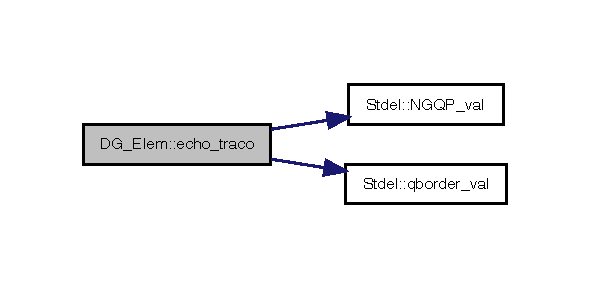
\includegraphics[width=283pt]{classDG__Elem_ab5d89b8f7625699239440bfd0e8ec6e6_cgraph}
\end{center}
\end{figure}
Here is the caller graph for this function\+:
\nopagebreak
\begin{figure}[H]
\begin{center}
\leavevmode
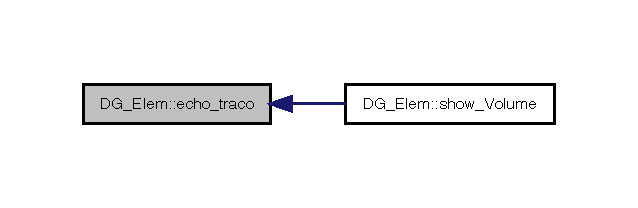
\includegraphics[width=306pt]{classDG__Elem_ab5d89b8f7625699239440bfd0e8ec6e6_icgraph}
\end{center}
\end{figure}
\mbox{\Hypertarget{classPhElem_a11a736e86c5b40e5b0a4c84754f2b066}\label{classPhElem_a11a736e86c5b40e5b0a4c84754f2b066}} 
\index{D\+G\+\_\+\+Elem@{D\+G\+\_\+\+Elem}!escrever\+\_\+restart@{escrever\+\_\+restart}}
\index{escrever\+\_\+restart@{escrever\+\_\+restart}!D\+G\+\_\+\+Elem@{D\+G\+\_\+\+Elem}}
\subsubsection{\texorpdfstring{escrever\+\_\+restart()}{escrever\_restart()}}
{\footnotesize\ttfamily void \hyperlink{classPhElem}{Ph\+Elem}$<$ Num\+Variaveis $>$\+::escrever\+\_\+restart (\begin{DoxyParamCaption}\item[{F\+I\+LE $\ast$}]{fout }\end{DoxyParamCaption})\hspace{0.3cm}{\ttfamily [inherited]}}



Definition at line 242 of file Ph\+Elem.\+hpp.



References Ph\+Elem$<$ Num\+Variaveis $>$\+::numn, and Ph\+Elem$<$ Num\+Variaveis $>$\+::u0.

\mbox{\Hypertarget{classDG__Elem_af91d2d61c97fae30b8dfc6db67433094}\label{classDG__Elem_af91d2d61c97fae30b8dfc6db67433094}} 
\index{D\+G\+\_\+\+Elem@{D\+G\+\_\+\+Elem}!finaliza\+\_\+vetores@{finaliza\+\_\+vetores}}
\index{finaliza\+\_\+vetores@{finaliza\+\_\+vetores}!D\+G\+\_\+\+Elem@{D\+G\+\_\+\+Elem}}
\subsubsection{\texorpdfstring{finaliza\+\_\+vetores()}{finaliza\_vetores()}}
{\footnotesize\ttfamily void D\+G\+\_\+\+Elem\+::finaliza\+\_\+vetores (\begin{DoxyParamCaption}{ }\end{DoxyParamCaption})}



Definition at line 1650 of file D\+G\+\_\+\+Elem.\+cpp.



References Grad\+Phi, Jb, Ph\+Elem$<$ 2 $>$\+::\+JV, Laplaciano\+Phi, Mass\+\_\+sn, Ph\+Elem$<$ 2 $>$\+::ndim, Ph\+Elem$<$ 2 $>$\+::numborders, Ph\+Elem$<$ 2 $>$\+::numn, Stdel\+::\+P\+\_\+val(), Ph\+Elem$<$ 2 $>$\+::ptr\+\_\+stdel, pwa, sna, Ph\+Elem$<$ 2 $>$\+::stgbtrbmapM, Ph\+Elem$<$ 2 $>$\+::stgbtrbmapP, Tr\+Grad\+Phi, Tr\+Kgrad\+\_\+pc, Tr\+Kgrad\+\_\+pw, Tr\+Kgrad\+\_\+sn, Tr\+Kgrad\+Phi\+\_\+n, Tr\+Phi, Trpw, Trsn, Ph\+Elem$<$ 2 $>$\+::u0, Ph\+Elem$<$ 2 $>$\+::usave, and Ph\+Elem$<$ 2 $>$\+::vetores\+\_\+iniciados.



Referenced by show\+\_\+\+Volume(), and D\+G\+\_\+\+Prob\+::$\sim$\+D\+G\+\_\+\+Prob().

Here is the call graph for this function\+:
\nopagebreak
\begin{figure}[H]
\begin{center}
\leavevmode
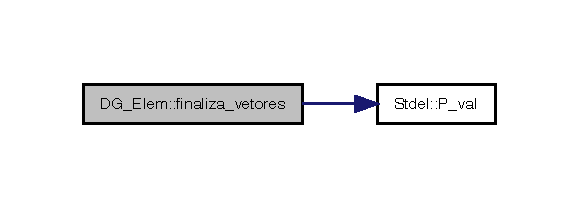
\includegraphics[width=278pt]{classDG__Elem_af91d2d61c97fae30b8dfc6db67433094_cgraph}
\end{center}
\end{figure}
Here is the caller graph for this function\+:
\nopagebreak
\begin{figure}[H]
\begin{center}
\leavevmode
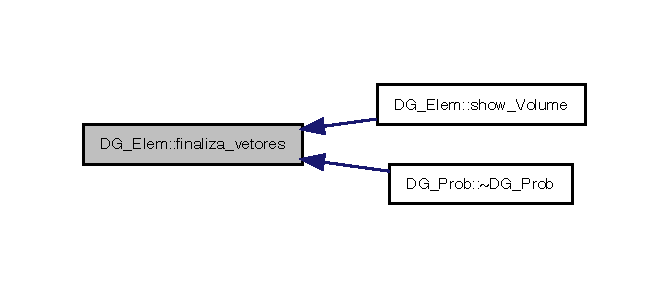
\includegraphics[width=321pt]{classDG__Elem_af91d2d61c97fae30b8dfc6db67433094_icgraph}
\end{center}
\end{figure}
\mbox{\Hypertarget{classPhElem_a19299ae55f9faef322a1d21d7e9b2a88}\label{classPhElem_a19299ae55f9faef322a1d21d7e9b2a88}} 
\index{D\+G\+\_\+\+Elem@{D\+G\+\_\+\+Elem}!gbnmap\+\_\+aresta@{gbnmap\+\_\+aresta}}
\index{gbnmap\+\_\+aresta@{gbnmap\+\_\+aresta}!D\+G\+\_\+\+Elem@{D\+G\+\_\+\+Elem}}
\subsubsection{\texorpdfstring{gbnmap\+\_\+aresta()}{gbnmap\_aresta()}}
{\footnotesize\ttfamily void \hyperlink{classPhElem}{Ph\+Elem}$<$ Num\+Variaveis $>$\+::gbnmap\+\_\+aresta (\begin{DoxyParamCaption}\item[{const int \&}]{aresta,  }\item[{const int \&}]{sinal,  }\item[{const int \&}]{ivar,  }\item[{const int \&}]{count,  }\item[{int \&}]{inc }\end{DoxyParamCaption})\hspace{0.3cm}{\ttfamily [inherited]}}



Definition at line 1719 of file Ph\+Elem.\+hpp.



References aux, Ph\+Elem$<$ Num\+Variaveis $>$\+::gbnmap, Ph\+Elem$<$ Num\+Variaveis $>$\+::ptr\+\_\+stdel, Ph\+Elem$<$ Num\+Variaveis $>$\+::sgn, Stdel\+::show\+\_\+emapi(), Stdel\+::show\+\_\+emapv(), and Ph\+Elem$<$ Num\+Variaveis $>$\+::sinal.

\mbox{\Hypertarget{classPhElem_af545eccd164b2fc7ca104afff13a50c6}\label{classPhElem_af545eccd164b2fc7ca104afff13a50c6}} 
\index{D\+G\+\_\+\+Elem@{D\+G\+\_\+\+Elem}!gbnmap\+\_\+arestas@{gbnmap\+\_\+arestas}}
\index{gbnmap\+\_\+arestas@{gbnmap\+\_\+arestas}!D\+G\+\_\+\+Elem@{D\+G\+\_\+\+Elem}}
\subsubsection{\texorpdfstring{gbnmap\+\_\+arestas()}{gbnmap\_arestas()}}
{\footnotesize\ttfamily void \hyperlink{classPhElem}{Ph\+Elem}$<$ Num\+Variaveis $>$\+::gbnmap\+\_\+arestas (\begin{DoxyParamCaption}\item[{const int}]{aresta\+\_\+vec\mbox{[}$\,$\mbox{]},  }\item[{const int \&}]{ivar }\end{DoxyParamCaption})\hspace{0.3cm}{\ttfamily [inherited]}}



Definition at line 1832 of file Ph\+Elem.\+hpp.



References a, Stdel\+::aresta\+\_\+lvert(), Ph\+Elem$<$ Num\+Variaveis $>$\+::aresta\+\_\+map, aux, Ph\+Elem$<$ Num\+Variaveis $>$\+::gbnmap, Ph\+Elem$<$ Num\+Variaveis $>$\+::nume, Ph\+Elem$<$ Num\+Variaveis $>$\+::ptr\+\_\+stdel, Ph\+Elem$<$ Num\+Variaveis $>$\+::sgn, Stdel\+::show\+\_\+emapi(), Stdel\+::show\+\_\+emapv(), Ph\+Elem$<$ Num\+Variaveis $>$\+::sinal, and Ph\+Elem$<$ Num\+Variaveis $>$\+::\+Vert\+\_\+map.

\mbox{\Hypertarget{classPhElem_ad355231f4e2807541c62212647c44b3e}\label{classPhElem_ad355231f4e2807541c62212647c44b3e}} 
\index{D\+G\+\_\+\+Elem@{D\+G\+\_\+\+Elem}!gbnmap\+\_\+faces@{gbnmap\+\_\+faces}}
\index{gbnmap\+\_\+faces@{gbnmap\+\_\+faces}!D\+G\+\_\+\+Elem@{D\+G\+\_\+\+Elem}}
\subsubsection{\texorpdfstring{gbnmap\+\_\+faces()}{gbnmap\_faces()}}
{\footnotesize\ttfamily void \hyperlink{classPhElem}{Ph\+Elem}$<$ Num\+Variaveis $>$\+::gbnmap\+\_\+faces (\begin{DoxyParamCaption}\item[{const int}]{face\+\_\+vec\mbox{[}$\,$\mbox{]},  }\item[{const int \&}]{ivar }\end{DoxyParamCaption})\hspace{0.3cm}{\ttfamily [inherited]}}



Definition at line 1754 of file Ph\+Elem.\+hpp.



References aux1, Stdel\+::face\+\_\+lvert(), Ph\+Elem$<$ Num\+Variaveis $>$\+::face\+\_\+map, Ph\+Elem$<$ Num\+Variaveis $>$\+::gbnmap, Ph\+Elem$<$ Num\+Variaveis $>$\+::numf, Stdel\+::\+P\+\_\+val(), Ph\+Elem$<$ Num\+Variaveis $>$\+::ptr\+\_\+stdel, quad\+\_\+ordem(), Ph\+Elem$<$ Num\+Variaveis $>$\+::sgn, Stdel\+::show\+\_\+fd0(), Stdel\+::show\+\_\+fd1(), Stdel\+::show\+\_\+fv2(), Stdel\+::show\+\_\+ind\+\_\+mode(), Stdel\+::show\+\_\+nvf(), Ph\+Elem$<$ Num\+Variaveis $>$\+::sinal, and Ph\+Elem$<$ Num\+Variaveis $>$\+::\+Vert\+\_\+map.

\mbox{\Hypertarget{classPhElem_ae6f35113c182e2678646552e6c4a752c}\label{classPhElem_ae6f35113c182e2678646552e6c4a752c}} 
\index{D\+G\+\_\+\+Elem@{D\+G\+\_\+\+Elem}!gbnmap\+\_\+interior@{gbnmap\+\_\+interior}}
\index{gbnmap\+\_\+interior@{gbnmap\+\_\+interior}!D\+G\+\_\+\+Elem@{D\+G\+\_\+\+Elem}}
\subsubsection{\texorpdfstring{gbnmap\+\_\+interior()}{gbnmap\_interior()}}
{\footnotesize\ttfamily void \hyperlink{classPhElem}{Ph\+Elem}$<$ Num\+Variaveis $>$\+::gbnmap\+\_\+interior (\begin{DoxyParamCaption}\item[{const int \&}]{ivar,  }\item[{int \&}]{count }\end{DoxyParamCaption})\hspace{0.3cm}{\ttfamily [inherited]}}



Definition at line 1742 of file Ph\+Elem.\+hpp.



References Ph\+Elem$<$ Num\+Variaveis $>$\+::gbnmap, Ph\+Elem$<$ Num\+Variaveis $>$\+::numb, Ph\+Elem$<$ Num\+Variaveis $>$\+::numn, and Ph\+Elem$<$ Num\+Variaveis $>$\+::sgn.

\mbox{\Hypertarget{classPhElem_ad8d5bac3d1866cfe20daec73fc405b05}\label{classPhElem_ad8d5bac3d1866cfe20daec73fc405b05}} 
\index{D\+G\+\_\+\+Elem@{D\+G\+\_\+\+Elem}!gbnmap\+\_\+vertices@{gbnmap\+\_\+vertices}}
\index{gbnmap\+\_\+vertices@{gbnmap\+\_\+vertices}!D\+G\+\_\+\+Elem@{D\+G\+\_\+\+Elem}}
\subsubsection{\texorpdfstring{gbnmap\+\_\+vertices()}{gbnmap\_vertices()}\hspace{0.1cm}{\footnotesize\ttfamily [1/2]}}
{\footnotesize\ttfamily void \hyperlink{classPhElem}{Ph\+Elem}$<$ Num\+Variaveis $>$\+::gbnmap\+\_\+vertices (\begin{DoxyParamCaption}\item[{std\+::vector$<$ std\+::vector$<$ int $>$$>$}]{gbn }\end{DoxyParamCaption})\hspace{0.3cm}{\ttfamily [inherited]}}



Definition at line 1696 of file Ph\+Elem.\+hpp.



References Ph\+Elem$<$ Num\+Variaveis $>$\+::gbnmap, Ph\+Elem$<$ Num\+Variaveis $>$\+::gbnmap\+\_\+vertices(), Ph\+Elem$<$ Num\+Variaveis $>$\+::numv, Ph\+Elem$<$ Num\+Variaveis $>$\+::sgn, and Ph\+Elem$<$ Num\+Variaveis $>$\+::\+Vert\+\_\+map.

\mbox{\Hypertarget{classPhElem_a75f80b321d33ea208ae2d35af1b8c4df}\label{classPhElem_a75f80b321d33ea208ae2d35af1b8c4df}} 
\index{D\+G\+\_\+\+Elem@{D\+G\+\_\+\+Elem}!gbnmap\+\_\+vertices@{gbnmap\+\_\+vertices}}
\index{gbnmap\+\_\+vertices@{gbnmap\+\_\+vertices}!D\+G\+\_\+\+Elem@{D\+G\+\_\+\+Elem}}
\subsubsection{\texorpdfstring{gbnmap\+\_\+vertices()}{gbnmap\_vertices()}\hspace{0.1cm}{\footnotesize\ttfamily [2/2]}}
{\footnotesize\ttfamily void \hyperlink{classPhElem}{Ph\+Elem}$<$ Num\+Variaveis $>$\+::gbnmap\+\_\+vertices (\begin{DoxyParamCaption}\item[{int $\ast$}]{gbn,  }\item[{const int \&}]{ivar }\end{DoxyParamCaption})\hspace{0.3cm}{\ttfamily [inherited]}}

\mbox{\Hypertarget{classPhElem_a35508e257e1675a912954f83cb4b6a3e}\label{classPhElem_a35508e257e1675a912954f83cb4b6a3e}} 
\index{D\+G\+\_\+\+Elem@{D\+G\+\_\+\+Elem}!get\+\_\+trace\+\_\+border\+\_\+map@{get\+\_\+trace\+\_\+border\+\_\+map}}
\index{get\+\_\+trace\+\_\+border\+\_\+map@{get\+\_\+trace\+\_\+border\+\_\+map}!D\+G\+\_\+\+Elem@{D\+G\+\_\+\+Elem}}
\subsubsection{\texorpdfstring{get\+\_\+trace\+\_\+border\+\_\+map()}{get\_trace\_border\_map()}}
{\footnotesize\ttfamily int \hyperlink{classPhElem}{Ph\+Elem}$<$ Num\+Variaveis $>$\+::get\+\_\+trace\+\_\+border\+\_\+map (\begin{DoxyParamCaption}\item[{const int \&}]{aresta }\end{DoxyParamCaption})\hspace{0.3cm}{\ttfamily [inherited]}}



Definition at line 520 of file Ph\+Elem.\+hpp.



References Ph\+Elem$<$ Num\+Variaveis $>$\+::gbtrbmap, Ph\+Elem$<$ Num\+Variaveis $>$\+::ptr\+\_\+stdel, Stdel\+::qborder\+\_\+val(), and qmax.

\mbox{\Hypertarget{classPhElem_a6f8258d7b66de04cd4d88f2c8af41541}\label{classPhElem_a6f8258d7b66de04cd4d88f2c8af41541}} 
\index{D\+G\+\_\+\+Elem@{D\+G\+\_\+\+Elem}!Imprimir\+\_\+valores@{Imprimir\+\_\+valores}}
\index{Imprimir\+\_\+valores@{Imprimir\+\_\+valores}!D\+G\+\_\+\+Elem@{D\+G\+\_\+\+Elem}}
\subsubsection{\texorpdfstring{Imprimir\+\_\+valores()}{Imprimir\_valores()}}
{\footnotesize\ttfamily void \hyperlink{classPhElem}{Ph\+Elem}$<$ Num\+Variaveis $>$\+::Imprimir\+\_\+valores (\begin{DoxyParamCaption}\item[{F\+I\+LE $\ast$}]{fileout,  }\item[{const int \&}]{npoints,  }\item[{const double}]{coord\mbox{[}$\,$\mbox{]} }\end{DoxyParamCaption})\hspace{0.3cm}{\ttfamily [inherited]}}

\mbox{\Hypertarget{classPhElem_afac13525ce0e8907ca74a7213aa72504}\label{classPhElem_afac13525ce0e8907ca74a7213aa72504}} 
\index{D\+G\+\_\+\+Elem@{D\+G\+\_\+\+Elem}!Increment\+\_\+field@{Increment\+\_\+field}}
\index{Increment\+\_\+field@{Increment\+\_\+field}!D\+G\+\_\+\+Elem@{D\+G\+\_\+\+Elem}}
\subsubsection{\texorpdfstring{Increment\+\_\+field()}{Increment\_field()}}
{\footnotesize\ttfamily void \hyperlink{classPhElem}{Ph\+Elem}$<$ Num\+Variaveis $>$\+::Increment\+\_\+field (\begin{DoxyParamCaption}\item[{const double}]{X\mbox{[}$\,$\mbox{]},  }\item[{const int \&}]{numf,  }\item[{const double}]{dt }\end{DoxyParamCaption})\hspace{0.3cm}{\ttfamily [inherited]}}

\mbox{\Hypertarget{classDG__Elem_af61130ab38851fa2ade53f9e3f2418bc}\label{classDG__Elem_af61130ab38851fa2ade53f9e3f2418bc}} 
\index{D\+G\+\_\+\+Elem@{D\+G\+\_\+\+Elem}!inicia\+\_\+funcoes\+\_\+na\+\_\+borda@{inicia\+\_\+funcoes\+\_\+na\+\_\+borda}}
\index{inicia\+\_\+funcoes\+\_\+na\+\_\+borda@{inicia\+\_\+funcoes\+\_\+na\+\_\+borda}!D\+G\+\_\+\+Elem@{D\+G\+\_\+\+Elem}}
\subsubsection{\texorpdfstring{inicia\+\_\+funcoes\+\_\+na\+\_\+borda()}{inicia\_funcoes\_na\_borda()}}
{\footnotesize\ttfamily void D\+G\+\_\+\+Elem\+::inicia\+\_\+funcoes\+\_\+na\+\_\+borda (\begin{DoxyParamCaption}\item[{\hyperlink{structEDGE}{E\+D\+GE} $\ast$}]{border }\end{DoxyParamCaption})}



Definition at line 44 of file D\+G\+\_\+\+Elem.\+cpp.



References Ph\+Elem$<$ 2 $>$\+::border\+\_\+num, Stdel\+::elem\+\_\+traces(), Stdel\+::eval\+\_\+\+Phi(), Stdel\+::\+Gradiente(), Grad\+Phi, Jb, Laplaciano\+Phi, n\+\_\+e, Ph\+Elem$<$ 2 $>$\+::ndim, Stdel\+::\+N\+G\+Q\+P\+\_\+val(), E\+D\+G\+E\+::normal, Ph\+Elem$<$ 2 $>$\+::numborders, Ph\+Elem$<$ 2 $>$\+::\+Num\+Local\+Vars, Ph\+Elem$<$ 2 $>$\+::numn, perm, pos, Ph\+Elem$<$ 2 $>$\+::ptr\+\_\+stdel, Ph\+Elem$<$ 2 $>$\+::ptvert, Stdel\+::qborder\+\_\+val(), qmax, Ph\+Elem$<$ 2 $>$\+::sinal, Tr\+Grad\+Phi, Tr\+Kgrad\+Phi\+\_\+n, Tr\+Phi, and Ph\+Elem$<$ 2 $>$\+::\+Vert\+\_\+map.



Referenced by D\+G\+\_\+\+Prob\+::\+D\+G\+\_\+initial\+\_\+conditions(), and show\+\_\+\+Volume().

Here is the call graph for this function\+:
\nopagebreak
\begin{figure}[H]
\begin{center}
\leavevmode
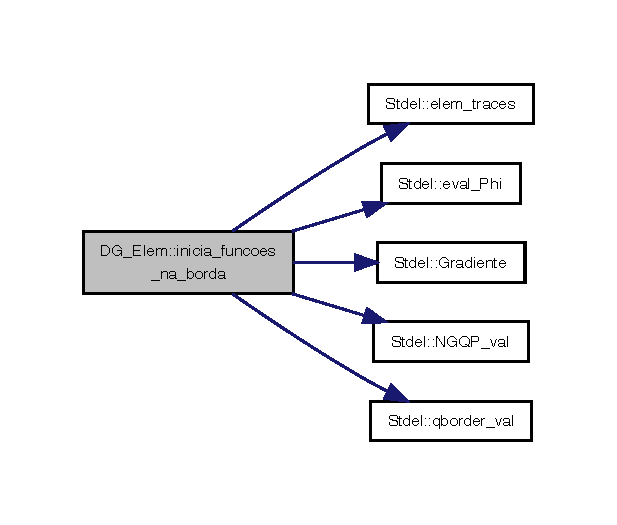
\includegraphics[width=296pt]{classDG__Elem_af61130ab38851fa2ade53f9e3f2418bc_cgraph}
\end{center}
\end{figure}
Here is the caller graph for this function\+:
\nopagebreak
\begin{figure}[H]
\begin{center}
\leavevmode
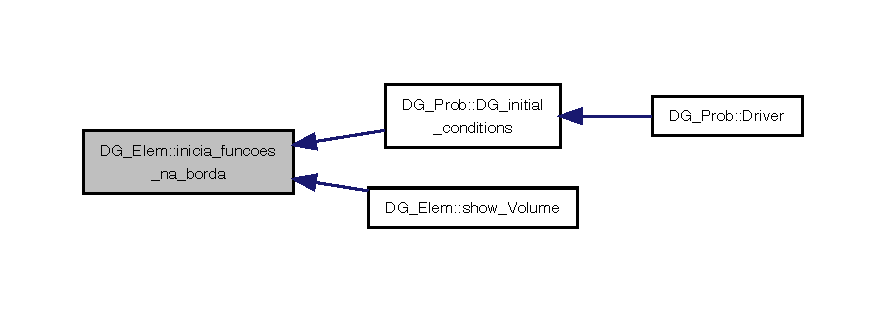
\includegraphics[width=350pt]{classDG__Elem_af61130ab38851fa2ade53f9e3f2418bc_icgraph}
\end{center}
\end{figure}
\mbox{\Hypertarget{classPhElem_a98449dc77f691781f54fc8798bea03a3}\label{classPhElem_a98449dc77f691781f54fc8798bea03a3}} 
\index{D\+G\+\_\+\+Elem@{D\+G\+\_\+\+Elem}!inicia\+\_\+gbnmap@{inicia\+\_\+gbnmap}}
\index{inicia\+\_\+gbnmap@{inicia\+\_\+gbnmap}!D\+G\+\_\+\+Elem@{D\+G\+\_\+\+Elem}}
\subsubsection{\texorpdfstring{inicia\+\_\+gbnmap()}{inicia\_gbnmap()}\hspace{0.1cm}{\footnotesize\ttfamily [1/2]}}
{\footnotesize\ttfamily void \hyperlink{classPhElem}{Ph\+Elem}$<$ Num\+Variaveis $>$\+::inicia\+\_\+gbnmap (\begin{DoxyParamCaption}\item[{int \&}]{count }\end{DoxyParamCaption})\hspace{0.3cm}{\ttfamily [inherited]}}



Definition at line 838 of file Ph\+Elem.\+hpp.



References Ph\+Elem$<$ Num\+Variaveis $>$\+::inicia\+\_\+gbnmap().

\mbox{\Hypertarget{classPhElem_a3ed7c7027c6fadd45f29eb7de33ee7fb}\label{classPhElem_a3ed7c7027c6fadd45f29eb7de33ee7fb}} 
\index{D\+G\+\_\+\+Elem@{D\+G\+\_\+\+Elem}!inicia\+\_\+gbnmap@{inicia\+\_\+gbnmap}}
\index{inicia\+\_\+gbnmap@{inicia\+\_\+gbnmap}!D\+G\+\_\+\+Elem@{D\+G\+\_\+\+Elem}}
\subsubsection{\texorpdfstring{inicia\+\_\+gbnmap()}{inicia\_gbnmap()}\hspace{0.1cm}{\footnotesize\ttfamily [2/2]}}
{\footnotesize\ttfamily void \hyperlink{classPhElem}{Ph\+Elem}$<$ Num\+Variaveis $>$\+::inicia\+\_\+gbnmap (\begin{DoxyParamCaption}\item[{const int \&}]{ivar,  }\item[{int \&}]{count }\end{DoxyParamCaption})\hspace{0.3cm}{\ttfamily [inherited]}}



Definition at line 846 of file Ph\+Elem.\+hpp.



References Ph\+Elem$<$ Num\+Variaveis $>$\+::gbnmap, Ph\+Elem$<$ Num\+Variaveis $>$\+::numn, and Ph\+Elem$<$ Num\+Variaveis $>$\+::sgn.

\mbox{\Hypertarget{classPhElem_a9b5610a7a12eddbc4a9f07429500a6da}\label{classPhElem_a9b5610a7a12eddbc4a9f07429500a6da}} 
\index{D\+G\+\_\+\+Elem@{D\+G\+\_\+\+Elem}!inicia\+\_\+gbtrbmap@{inicia\+\_\+gbtrbmap}}
\index{inicia\+\_\+gbtrbmap@{inicia\+\_\+gbtrbmap}!D\+G\+\_\+\+Elem@{D\+G\+\_\+\+Elem}}
\subsubsection{\texorpdfstring{inicia\+\_\+gbtrbmap()}{inicia\_gbtrbmap()}}
{\footnotesize\ttfamily void \hyperlink{classPhElem}{Ph\+Elem}$<$ Num\+Variaveis $>$\+::inicia\+\_\+gbtrbmap (\begin{DoxyParamCaption}\item[{int \&}]{count }\end{DoxyParamCaption})\hspace{0.3cm}{\ttfamily [inherited]}}



Definition at line 856 of file Ph\+Elem.\+hpp.



References Ph\+Elem$<$ Num\+Variaveis $>$\+::gbtrbmap, Ph\+Elem$<$ Num\+Variaveis $>$\+::numborders, Ph\+Elem$<$ Num\+Variaveis $>$\+::ptr\+\_\+stdel, Stdel\+::qborder\+\_\+val(), qmax, Ph\+Elem$<$ Num\+Variaveis $>$\+::stgbtrbmapM, and Ph\+Elem$<$ Num\+Variaveis $>$\+::stgbtrbmapP.

\mbox{\Hypertarget{classDG__Elem_a33d01f96cc0d00b6a1a1d4a817724b4c}\label{classDG__Elem_a33d01f96cc0d00b6a1a1d4a817724b4c}} 
\index{D\+G\+\_\+\+Elem@{D\+G\+\_\+\+Elem}!inicia\+\_\+tracos@{inicia\+\_\+tracos}}
\index{inicia\+\_\+tracos@{inicia\+\_\+tracos}!D\+G\+\_\+\+Elem@{D\+G\+\_\+\+Elem}}
\subsubsection{\texorpdfstring{inicia\+\_\+tracos()}{inicia\_tracos()}}
{\footnotesize\ttfamily void D\+G\+\_\+\+Elem\+::inicia\+\_\+tracos (\begin{DoxyParamCaption}\item[{\hyperlink{structEDGE}{E\+D\+GE} $\ast$}]{border }\end{DoxyParamCaption})}



Definition at line 158 of file D\+G\+\_\+\+Elem.\+cpp.



References Ph\+Elem$<$ 2 $>$\+::border\+\_\+num, Stdel\+::eval\+\_\+\+Phi(), Stdel\+::\+Gradiente(), Grad\+Phi, n\+\_\+e, Ph\+Elem$<$ 2 $>$\+::ndim, Stdel\+::\+N\+G\+Q\+P\+\_\+val(), E\+D\+G\+E\+::normal, Ph\+Elem$<$ 2 $>$\+::numborders, Ph\+Elem$<$ 2 $>$\+::\+Num\+Local\+Vars, Ph\+Elem$<$ 2 $>$\+::numn, perm, pos, Ph\+Elem$<$ 2 $>$\+::ptr\+\_\+stdel, Ph\+Elem$<$ 2 $>$\+::ptvert, Stdel\+::qborder\+\_\+val(), qmax, Ph\+Elem$<$ 2 $>$\+::sinal, Stdel\+::trace(), Tr\+Grad\+Phi, Tr\+Kgrad\+Phi\+\_\+n, Tr\+Phi, and Ph\+Elem$<$ 2 $>$\+::\+Vert\+\_\+map.



Referenced by show\+\_\+\+Volume().

Here is the call graph for this function\+:
\nopagebreak
\begin{figure}[H]
\begin{center}
\leavevmode
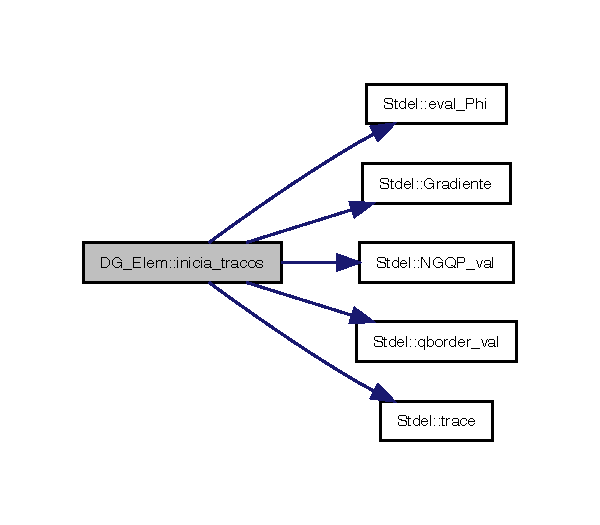
\includegraphics[width=288pt]{classDG__Elem_a33d01f96cc0d00b6a1a1d4a817724b4c_cgraph}
\end{center}
\end{figure}
Here is the caller graph for this function\+:
\nopagebreak
\begin{figure}[H]
\begin{center}
\leavevmode
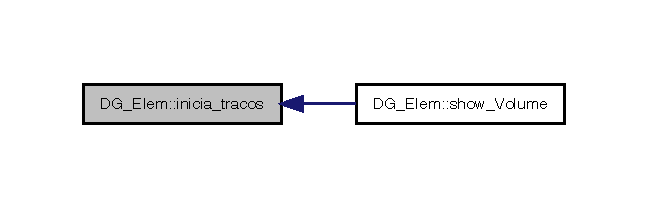
\includegraphics[width=311pt]{classDG__Elem_a33d01f96cc0d00b6a1a1d4a817724b4c_icgraph}
\end{center}
\end{figure}
\mbox{\Hypertarget{classDG__Elem_ac1ec1f962d6e1852f0adb01048c4c1f9}\label{classDG__Elem_ac1ec1f962d6e1852f0adb01048c4c1f9}} 
\index{D\+G\+\_\+\+Elem@{D\+G\+\_\+\+Elem}!inicia\+\_\+vetores@{inicia\+\_\+vetores}}
\index{inicia\+\_\+vetores@{inicia\+\_\+vetores}!D\+G\+\_\+\+Elem@{D\+G\+\_\+\+Elem}}
\subsubsection{\texorpdfstring{inicia\+\_\+vetores()}{inicia\_vetores()}}
{\footnotesize\ttfamily void D\+G\+\_\+\+Elem\+::inicia\+\_\+vetores (\begin{DoxyParamCaption}{ }\end{DoxyParamCaption})}



Definition at line 1463 of file D\+G\+\_\+\+Elem.\+cpp.



References Ph\+Elem$<$ 2 $>$\+::compute\+\_\+\+J\+V(), Grad\+Phi, Jb, Ph\+Elem$<$ 2 $>$\+::\+JV, Laplaciano\+Phi, Mass\+\_\+sn, Ph\+Elem$<$ 2 $>$\+::ndim, Stdel\+::\+N\+G\+Q\+P\+\_\+val(), Ph\+Elem$<$ 2 $>$\+::numborders, Ph\+Elem$<$ 2 $>$\+::\+Num\+Local\+Vars, Ph\+Elem$<$ 2 $>$\+::numn, Ph\+Elem$<$ 2 $>$\+::ptr\+\_\+stdel, pwa, Stdel\+::qborder\+\_\+val(), qmax, sna, Tr\+Grad\+Phi, Tr\+Kgrad\+\_\+pc, Tr\+Kgrad\+\_\+pw, Tr\+Kgrad\+\_\+sn, Tr\+Kgrad\+Phi\+\_\+n, Tr\+Phi, Trpw, Trsn, Ph\+Elem$<$ 2 $>$\+::u0, Ph\+Elem$<$ 2 $>$\+::usave, and Ph\+Elem$<$ 2 $>$\+::vetores\+\_\+iniciados.



Referenced by D\+G\+\_\+\+Prob\+::\+D\+G\+\_\+initial\+\_\+conditions(), D\+G\+\_\+\+Prob\+::projetar\+\_\+\+C0(), and $\sim$\+D\+G\+\_\+\+Elem().

Here is the call graph for this function\+:
\nopagebreak
\begin{figure}[H]
\begin{center}
\leavevmode
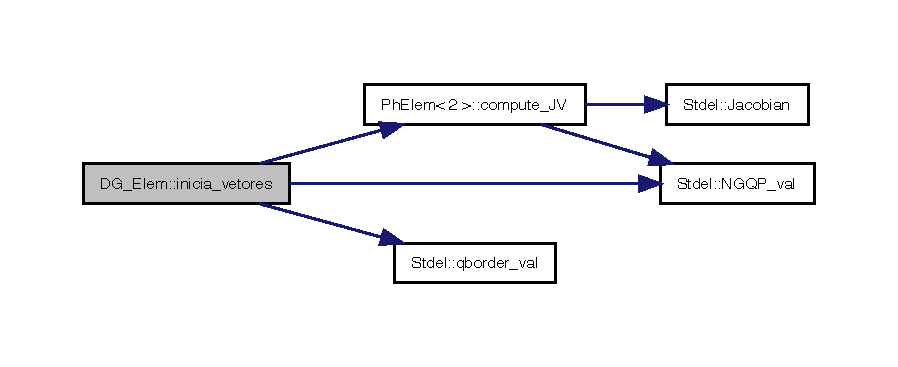
\includegraphics[width=350pt]{classDG__Elem_ac1ec1f962d6e1852f0adb01048c4c1f9_cgraph}
\end{center}
\end{figure}
Here is the caller graph for this function\+:
\nopagebreak
\begin{figure}[H]
\begin{center}
\leavevmode
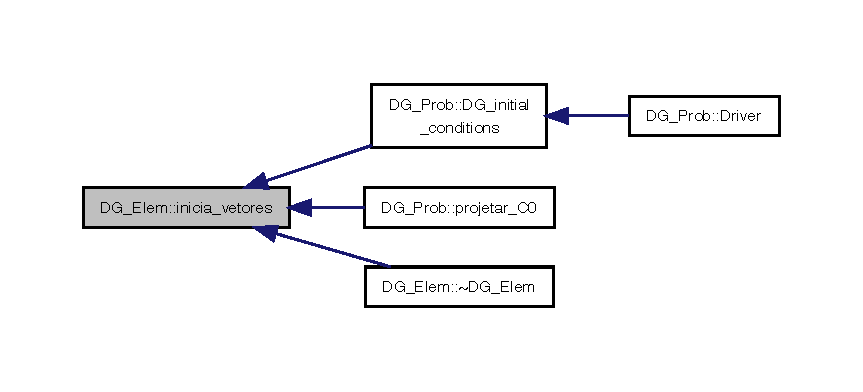
\includegraphics[width=350pt]{classDG__Elem_ac1ec1f962d6e1852f0adb01048c4c1f9_icgraph}
\end{center}
\end{figure}
\mbox{\Hypertarget{classPhElem_a3064c3377eb3f81d63f43969a3c958ee}\label{classPhElem_a3064c3377eb3f81d63f43969a3c958ee}} 
\index{D\+G\+\_\+\+Elem@{D\+G\+\_\+\+Elem}!K\+\_\+\+Imisc2F@{K\+\_\+\+Imisc2F}}
\index{K\+\_\+\+Imisc2F@{K\+\_\+\+Imisc2F}!D\+G\+\_\+\+Elem@{D\+G\+\_\+\+Elem}}
\subsubsection{\texorpdfstring{K\+\_\+\+Imisc2\+F()}{K\_Imisc2F()}}
{\footnotesize\ttfamily double \hyperlink{classPhElem}{Ph\+Elem}$<$ Num\+Variaveis $>$\+::K\+\_\+\+Imisc2F (\begin{DoxyParamCaption}\item[{const int \&}]{i,  }\item[{const int \&}]{j }\end{DoxyParamCaption})\hspace{0.3cm}{\ttfamily [inherited]}}

\mbox{\Hypertarget{classPhElem_afdbe06fb407dc4c474b886ed219de195}\label{classPhElem_afdbe06fb407dc4c474b886ed219de195}} 
\index{D\+G\+\_\+\+Elem@{D\+G\+\_\+\+Elem}!Kcomp@{Kcomp}}
\index{Kcomp@{Kcomp}!D\+G\+\_\+\+Elem@{D\+G\+\_\+\+Elem}}
\subsubsection{\texorpdfstring{Kcomp()}{Kcomp()}}
{\footnotesize\ttfamily double \hyperlink{classPhElem}{Ph\+Elem}$<$ Num\+Variaveis $>$\+::Kcomp (\begin{DoxyParamCaption}\item[{const int \&}]{i,  }\item[{const int \&}]{j }\end{DoxyParamCaption})\hspace{0.3cm}{\ttfamily [inherited]}}



Definition at line 183 of file Elastostatica.\+cpp.



References Ph\+Elem$<$ Num\+Variaveis $>$\+::sgn.

\mbox{\Hypertarget{classPhElem_a0209eb7e6db7b0b541b51c46269ee9b6}\label{classPhElem_a0209eb7e6db7b0b541b51c46269ee9b6}} 
\index{D\+G\+\_\+\+Elem@{D\+G\+\_\+\+Elem}!ler\+\_\+restart@{ler\+\_\+restart}}
\index{ler\+\_\+restart@{ler\+\_\+restart}!D\+G\+\_\+\+Elem@{D\+G\+\_\+\+Elem}}
\subsubsection{\texorpdfstring{ler\+\_\+restart()}{ler\_restart()}}
{\footnotesize\ttfamily void \hyperlink{classPhElem}{Ph\+Elem}$<$ Num\+Variaveis $>$\+::ler\+\_\+restart (\begin{DoxyParamCaption}\item[{F\+I\+LE $\ast$}]{fin }\end{DoxyParamCaption})\hspace{0.3cm}{\ttfamily [inherited]}}



Definition at line 252 of file Ph\+Elem.\+hpp.



References Ph\+Elem$<$ Num\+Variaveis $>$\+::numn, and Ph\+Elem$<$ Num\+Variaveis $>$\+::u0.

\mbox{\Hypertarget{classPhElem_ad0a2992e6d206b6a351da8847a9dd69a}\label{classPhElem_ad0a2992e6d206b6a351da8847a9dd69a}} 
\index{D\+G\+\_\+\+Elem@{D\+G\+\_\+\+Elem}!ler\+\_\+restart\+\_\+buffer@{ler\+\_\+restart\+\_\+buffer}}
\index{ler\+\_\+restart\+\_\+buffer@{ler\+\_\+restart\+\_\+buffer}!D\+G\+\_\+\+Elem@{D\+G\+\_\+\+Elem}}
\subsubsection{\texorpdfstring{ler\+\_\+restart\+\_\+buffer()}{ler\_restart\_buffer()}}
{\footnotesize\ttfamily void \hyperlink{classPhElem}{Ph\+Elem}$<$ Num\+Variaveis $>$\+::ler\+\_\+restart\+\_\+buffer (\begin{DoxyParamCaption}\item[{F\+I\+LE $\ast$}]{fin,  }\item[{double $\ast$}]{buff,  }\item[{int \&}]{count }\end{DoxyParamCaption})\hspace{0.3cm}{\ttfamily [inherited]}}



Definition at line 261 of file Ph\+Elem.\+hpp.



References Ph\+Elem$<$ Num\+Variaveis $>$\+::numn.

\mbox{\Hypertarget{classPhElem_ac59f1cbe0962524e3aa5eced9a4393f6}\label{classPhElem_ac59f1cbe0962524e3aa5eced9a4393f6}} 
\index{D\+G\+\_\+\+Elem@{D\+G\+\_\+\+Elem}!make\+\_\+\+K\+\_\+\+Elast2D@{make\+\_\+\+K\+\_\+\+Elast2D}}
\index{make\+\_\+\+K\+\_\+\+Elast2D@{make\+\_\+\+K\+\_\+\+Elast2D}!D\+G\+\_\+\+Elem@{D\+G\+\_\+\+Elem}}
\subsubsection{\texorpdfstring{make\+\_\+\+K\+\_\+\+Elast2\+D()}{make\_K\_Elast2D()}}
{\footnotesize\ttfamily void \hyperlink{classPhElem}{Ph\+Elem}$<$ Num\+Variaveis $>$\+::make\+\_\+\+K\+\_\+\+Elast2D (\begin{DoxyParamCaption}\item[{const double}]{lambda,  }\item[{const double}]{mu,  }\item[{double $\ast$$\ast$}]{K }\end{DoxyParamCaption})\hspace{0.3cm}{\ttfamily [inherited]}}



Definition at line 7 of file Elastostatica.\+cpp.



References aaux, aux, Ph\+Elem$<$ Num\+Variaveis $>$\+::gbnmap, Ph\+Elem$<$ Num\+Variaveis $>$\+::\+JV, m, n0, and Ph\+Elem$<$ Num\+Variaveis $>$\+::ptvert.

\mbox{\Hypertarget{classPhElem_ae0418a5de14872e80fe4f9ffd9dd4fdd}\label{classPhElem_ae0418a5de14872e80fe4f9ffd9dd4fdd}} 
\index{D\+G\+\_\+\+Elem@{D\+G\+\_\+\+Elem}!make\+\_\+\+K\+\_\+\+Imiscivel2F@{make\+\_\+\+K\+\_\+\+Imiscivel2F}}
\index{make\+\_\+\+K\+\_\+\+Imiscivel2F@{make\+\_\+\+K\+\_\+\+Imiscivel2F}!D\+G\+\_\+\+Elem@{D\+G\+\_\+\+Elem}}
\subsubsection{\texorpdfstring{make\+\_\+\+K\+\_\+\+Imiscivel2\+F()}{make\_K\_Imiscivel2F()}}
{\footnotesize\ttfamily void \hyperlink{classPhElem}{Ph\+Elem}$<$ Num\+Variaveis $>$\+::make\+\_\+\+K\+\_\+\+Imiscivel2F (\begin{DoxyParamCaption}\item[{const double}]{,  }\item[{const double}]{,  }\item[{const double}]{,  }\item[{const double}]{,  }\item[{const double}]{\mbox{[}$\,$\mbox{]},  }\item[{double($\ast$)(double)}]{,  }\item[{double($\ast$)(double)}]{,  }\item[{double($\ast$)(double)}]{ }\end{DoxyParamCaption})\hspace{0.3cm}{\ttfamily [inherited]}}

\mbox{\Hypertarget{classPhElem_a1223b3e50580a1a7959e5f3b665d0761}\label{classPhElem_a1223b3e50580a1a7959e5f3b665d0761}} 
\index{D\+G\+\_\+\+Elem@{D\+G\+\_\+\+Elem}!make\+\_\+\+Kcomp\+\_\+\+Elast2D@{make\+\_\+\+Kcomp\+\_\+\+Elast2D}}
\index{make\+\_\+\+Kcomp\+\_\+\+Elast2D@{make\+\_\+\+Kcomp\+\_\+\+Elast2D}!D\+G\+\_\+\+Elem@{D\+G\+\_\+\+Elem}}
\subsubsection{\texorpdfstring{make\+\_\+\+Kcomp\+\_\+\+Elast2\+D()}{make\_Kcomp\_Elast2D()}}
{\footnotesize\ttfamily void \hyperlink{classPhElem}{Ph\+Elem}$<$ Num\+Variaveis $>$\+::make\+\_\+\+Kcomp\+\_\+\+Elast2D (\begin{DoxyParamCaption}\item[{const double}]{lambda,  }\item[{const double}]{mu }\end{DoxyParamCaption})\hspace{0.3cm}{\ttfamily [inherited]}}



Definition at line 197 of file Elastostatica.\+cpp.



References aux, B(), C(), e, force0(), Ph\+Elem$<$ Num\+Variaveis $>$\+::make\+\_\+\+K\+\_\+\+Elast2\+D(), Ph\+Elem$<$ Num\+Variaveis $>$\+::make\+\_\+vector(), and n0.

\mbox{\Hypertarget{classPhElem_a1ce74128a48a212028f644a68ce8edc0}\label{classPhElem_a1ce74128a48a212028f644a68ce8edc0}} 
\index{D\+G\+\_\+\+Elem@{D\+G\+\_\+\+Elem}!make\+\_\+\+Kcomp\+\_\+\+Elast2\+D\+\_\+dyn@{make\+\_\+\+Kcomp\+\_\+\+Elast2\+D\+\_\+dyn}}
\index{make\+\_\+\+Kcomp\+\_\+\+Elast2\+D\+\_\+dyn@{make\+\_\+\+Kcomp\+\_\+\+Elast2\+D\+\_\+dyn}!D\+G\+\_\+\+Elem@{D\+G\+\_\+\+Elem}}
\subsubsection{\texorpdfstring{make\+\_\+\+Kcomp\+\_\+\+Elast2\+D\+\_\+dyn()}{make\_Kcomp\_Elast2D\_dyn()}}
{\footnotesize\ttfamily void \hyperlink{classPhElem}{Ph\+Elem}$<$ Num\+Variaveis $>$\+::make\+\_\+\+Kcomp\+\_\+\+Elast2\+D\+\_\+dyn (\begin{DoxyParamCaption}\item[{const double}]{lambda,  }\item[{const double}]{mu,  }\item[{const double}]{a\mbox{[}$\,$\mbox{]} }\end{DoxyParamCaption})\hspace{0.3cm}{\ttfamily [inherited]}}



Definition at line 386 of file Elastodinamica2\+D.\+cpp.



References aux, and n0.

\mbox{\Hypertarget{classPhElem_ae538fb941f4cedc88e27dd28f2460bb5}\label{classPhElem_ae538fb941f4cedc88e27dd28f2460bb5}} 
\index{D\+G\+\_\+\+Elem@{D\+G\+\_\+\+Elem}!make\+\_\+\+Mass\+Matrices@{make\+\_\+\+Mass\+Matrices}}
\index{make\+\_\+\+Mass\+Matrices@{make\+\_\+\+Mass\+Matrices}!D\+G\+\_\+\+Elem@{D\+G\+\_\+\+Elem}}
\subsubsection{\texorpdfstring{make\+\_\+\+Mass\+Matrices()}{make\_MassMatrices()}}
{\footnotesize\ttfamily void \hyperlink{classPhElem}{Ph\+Elem}$<$ Num\+Variaveis $>$\+::make\+\_\+\+Mass\+Matrices (\begin{DoxyParamCaption}{ }\end{DoxyParamCaption})\hspace{0.3cm}{\ttfamily [inherited]}}

\mbox{\Hypertarget{classPhElem_a5051606f1d1e914d52d3de8655195c9f}\label{classPhElem_a5051606f1d1e914d52d3de8655195c9f}} 
\index{D\+G\+\_\+\+Elem@{D\+G\+\_\+\+Elem}!make\+\_\+vector@{make\+\_\+vector}}
\index{make\+\_\+vector@{make\+\_\+vector}!D\+G\+\_\+\+Elem@{D\+G\+\_\+\+Elem}}
\subsubsection{\texorpdfstring{make\+\_\+vector()}{make\_vector()}}
{\footnotesize\ttfamily void \hyperlink{classPhElem}{Ph\+Elem}$<$ Num\+Variaveis $>$\+::make\+\_\+vector (\begin{DoxyParamCaption}\item[{const int \&}]{ia,  }\item[{double($\ast$)(double, double, double)}]{f }\end{DoxyParamCaption})\hspace{0.3cm}{\ttfamily [inherited]}}

\mbox{\Hypertarget{classPhElem_ad5732b2fb83ab0d9a2de7678391f87c4}\label{classPhElem_ad5732b2fb83ab0d9a2de7678391f87c4}} 
\index{D\+G\+\_\+\+Elem@{D\+G\+\_\+\+Elem}!make\+\_\+vector\+\_\+\+Elast2\+D\+\_\+dyn@{make\+\_\+vector\+\_\+\+Elast2\+D\+\_\+dyn}}
\index{make\+\_\+vector\+\_\+\+Elast2\+D\+\_\+dyn@{make\+\_\+vector\+\_\+\+Elast2\+D\+\_\+dyn}!D\+G\+\_\+\+Elem@{D\+G\+\_\+\+Elem}}
\subsubsection{\texorpdfstring{make\+\_\+vector\+\_\+\+Elast2\+D\+\_\+dyn()}{make\_vector\_Elast2D\_dyn()}}
{\footnotesize\ttfamily void \hyperlink{classPhElem}{Ph\+Elem}$<$ Num\+Variaveis $>$\+::make\+\_\+vector\+\_\+\+Elast2\+D\+\_\+dyn (\begin{DoxyParamCaption}\item[{const double}]{a\mbox{[}$\,$\mbox{]} }\end{DoxyParamCaption})\hspace{0.3cm}{\ttfamily [inherited]}}



Definition at line 369 of file Elastodinamica2\+D.\+cpp.



References aux.

\mbox{\Hypertarget{classPhElem_a5f08c96b39a608ac8500897535998d52}\label{classPhElem_a5f08c96b39a608ac8500897535998d52}} 
\index{D\+G\+\_\+\+Elem@{D\+G\+\_\+\+Elem}!make\+\_\+\+Vector\+\_\+\+Eq\+\_\+\+S1@{make\+\_\+\+Vector\+\_\+\+Eq\+\_\+\+S1}}
\index{make\+\_\+\+Vector\+\_\+\+Eq\+\_\+\+S1@{make\+\_\+\+Vector\+\_\+\+Eq\+\_\+\+S1}!D\+G\+\_\+\+Elem@{D\+G\+\_\+\+Elem}}
\subsubsection{\texorpdfstring{make\+\_\+\+Vector\+\_\+\+Eq\+\_\+\+S1()}{make\_Vector\_Eq\_S1()}}
{\footnotesize\ttfamily void \hyperlink{classPhElem}{Ph\+Elem}$<$ Num\+Variaveis $>$\+::make\+\_\+\+Vector\+\_\+\+Eq\+\_\+\+S1 (\begin{DoxyParamCaption}\item[{const double}]{,  }\item[{const double}]{,  }\item[{const double}]{,  }\item[{const double}]{,  }\item[{const double}]{\mbox{[}3\mbox{]},  }\item[{double($\ast$)(double)}]{ }\end{DoxyParamCaption})\hspace{0.3cm}{\ttfamily [inherited]}}

\mbox{\Hypertarget{classPhElem_a6b7f26c842b4f6b54782c6ddaa4fd6d6}\label{classPhElem_a6b7f26c842b4f6b54782c6ddaa4fd6d6}} 
\index{D\+G\+\_\+\+Elem@{D\+G\+\_\+\+Elem}!map@{map}}
\index{map@{map}!D\+G\+\_\+\+Elem@{D\+G\+\_\+\+Elem}}
\subsubsection{\texorpdfstring{map()}{map()}}
{\footnotesize\ttfamily int \hyperlink{classPhElem}{Ph\+Elem}$<$ Num\+Variaveis $>$\+::map (\begin{DoxyParamCaption}\item[{const int \&}]{var,  }\item[{const int \&}]{no\+\_\+local }\end{DoxyParamCaption})\hspace{0.3cm}{\ttfamily [inherited]}}



Definition at line 573 of file Ph\+Elem.\+hpp.



References Ph\+Elem$<$ Num\+Variaveis $>$\+::gbnmap.

\mbox{\Hypertarget{classPhElem_aa53cc9dad058e9dbebfb971bdabe80fc}\label{classPhElem_aa53cc9dad058e9dbebfb971bdabe80fc}} 
\index{D\+G\+\_\+\+Elem@{D\+G\+\_\+\+Elem}!mapa\+\_\+inverso@{mapa\+\_\+inverso}}
\index{mapa\+\_\+inverso@{mapa\+\_\+inverso}!D\+G\+\_\+\+Elem@{D\+G\+\_\+\+Elem}}
\subsubsection{\texorpdfstring{mapa\+\_\+inverso()}{mapa\_inverso()}}
{\footnotesize\ttfamily void \hyperlink{classPhElem}{Ph\+Elem}$<$ Num\+Variaveis $>$\+::mapa\+\_\+inverso (\begin{DoxyParamCaption}\item[{const int \&}]{ivar,  }\item[{const double}]{X\mbox{[}$\,$\mbox{]} }\end{DoxyParamCaption})\hspace{0.3cm}{\ttfamily [inherited]}}



Definition at line 280 of file Ph\+Elem.\+hpp.



References Ph\+Elem$<$ Num\+Variaveis $>$\+::gbnmap, Ph\+Elem$<$ Num\+Variaveis $>$\+::numn, and Ph\+Elem$<$ Num\+Variaveis $>$\+::u0.

\mbox{\Hypertarget{classPhElem_a857f4ffbef27f0ef054f59eceffbad27}\label{classPhElem_a857f4ffbef27f0ef054f59eceffbad27}} 
\index{D\+G\+\_\+\+Elem@{D\+G\+\_\+\+Elem}!Neumann@{Neumann}}
\index{Neumann@{Neumann}!D\+G\+\_\+\+Elem@{D\+G\+\_\+\+Elem}}
\subsubsection{\texorpdfstring{Neumann()}{Neumann()}}
{\footnotesize\ttfamily void \hyperlink{classPhElem}{Ph\+Elem}$<$ Num\+Variaveis $>$\+::Neumann (\begin{DoxyParamCaption}\item[{const int \&}]{aresta,  }\item[{const int \&}]{varn,  }\item[{const double}]{rho1,  }\item[{const double}]{mu1,  }\item[{const double}]{rho2,  }\item[{const double}]{mu2,  }\item[{const double}]{gravidade\mbox{[}$\,$\mbox{]} }\end{DoxyParamCaption})\hspace{0.3cm}{\ttfamily [inherited]}}

\mbox{\Hypertarget{classPhElem_a638d823f66d1600cb948df872eb753c1}\label{classPhElem_a638d823f66d1600cb948df872eb753c1}} 
\index{D\+G\+\_\+\+Elem@{D\+G\+\_\+\+Elem}!P\+\_\+eval\+\_\+phys@{P\+\_\+eval\+\_\+phys}}
\index{P\+\_\+eval\+\_\+phys@{P\+\_\+eval\+\_\+phys}!D\+G\+\_\+\+Elem@{D\+G\+\_\+\+Elem}}
\subsubsection{\texorpdfstring{P\+\_\+eval\+\_\+phys()}{P\_eval\_phys()}}
{\footnotesize\ttfamily void \hyperlink{classPhElem}{Ph\+Elem}$<$ Num\+Variaveis $>$\+::P\+\_\+eval\+\_\+phys (\begin{DoxyParamCaption}\item[{const int \&}]{numf,  }\item[{double}]{f0\mbox{[}$\,$\mbox{]} }\end{DoxyParamCaption})\hspace{0.3cm}{\ttfamily [inherited]}}



Definition at line 617 of file Ph\+Elem.\+hpp.



References Stdel\+::eval\+G\+Q(), Ph\+Elem$<$ Num\+Variaveis $>$\+::numn, Ph\+Elem$<$ Num\+Variaveis $>$\+::ptr\+\_\+stdel, and Ph\+Elem$<$ Num\+Variaveis $>$\+::u0.

\mbox{\Hypertarget{classPhElem_ac5436d432516c731328134ac91b9a70b}\label{classPhElem_ac5436d432516c731328134ac91b9a70b}} 
\index{D\+G\+\_\+\+Elem@{D\+G\+\_\+\+Elem}!P\+\_\+eval\+\_\+print@{P\+\_\+eval\+\_\+print}}
\index{P\+\_\+eval\+\_\+print@{P\+\_\+eval\+\_\+print}!D\+G\+\_\+\+Elem@{D\+G\+\_\+\+Elem}}
\subsubsection{\texorpdfstring{P\+\_\+eval\+\_\+print()}{P\_eval\_print()}}
{\footnotesize\ttfamily void \hyperlink{classPhElem}{Ph\+Elem}$<$ Num\+Variaveis $>$\+::P\+\_\+eval\+\_\+print (\begin{DoxyParamCaption}\item[{const double}]{X\mbox{[}$\,$\mbox{]},  }\item[{const int \&}]{numf,  }\item[{F\+I\+LE $\ast$}]{fout,  }\item[{double($\ast$)(double, double, double)}]{ }\end{DoxyParamCaption})\hspace{0.3cm}{\ttfamily [inherited]}}

\mbox{\Hypertarget{classPhElem_ac3bc9b0559e940faa2404b1541d0c403}\label{classPhElem_ac3bc9b0559e940faa2404b1541d0c403}} 
\index{D\+G\+\_\+\+Elem@{D\+G\+\_\+\+Elem}!P\+\_\+eval\+\_\+print\+\_\+\+Elast2D@{P\+\_\+eval\+\_\+print\+\_\+\+Elast2D}}
\index{P\+\_\+eval\+\_\+print\+\_\+\+Elast2D@{P\+\_\+eval\+\_\+print\+\_\+\+Elast2D}!D\+G\+\_\+\+Elem@{D\+G\+\_\+\+Elem}}
\subsubsection{\texorpdfstring{P\+\_\+eval\+\_\+print\+\_\+\+Elast2\+D()}{P\_eval\_print\_Elast2D()}}
{\footnotesize\ttfamily void \hyperlink{classPhElem}{Ph\+Elem}$<$ Num\+Variaveis $>$\+::P\+\_\+eval\+\_\+print\+\_\+\+Elast2D (\begin{DoxyParamCaption}\item[{F\+I\+LE $\ast$}]{fout,  }\item[{const double}]{X\mbox{[}$\,$\mbox{]},  }\item[{double}]{lambda,  }\item[{double}]{mu }\end{DoxyParamCaption})\hspace{0.3cm}{\ttfamily [inherited]}}



Definition at line 88 of file Elastostatica.\+cpp.



References Ph\+Elem$<$ Num\+Variaveis $>$\+::b0, Ph\+Elem$<$ Num\+Variaveis $>$\+::gbnmap, Ph\+Elem$<$ Num\+Variaveis $>$\+::map(), Ph\+Elem$<$ Num\+Variaveis $>$\+::numf, Ph\+Elem$<$ Num\+Variaveis $>$\+::ptvert, Ph\+Elem$<$ Num\+Variaveis $>$\+::sgn, Ph\+Elem$<$ Num\+Variaveis $>$\+::u0, and Ph\+Elem$<$ Num\+Variaveis $>$\+::\+Vector\+Elast2\+D().

\mbox{\Hypertarget{classPhElem_a467c1ae6065913d0ec9828c9d055539a}\label{classPhElem_a467c1ae6065913d0ec9828c9d055539a}} 
\index{D\+G\+\_\+\+Elem@{D\+G\+\_\+\+Elem}!P\+\_\+eval\+\_\+print\+\_\+\+Elast2\+D\+\_\+dyn@{P\+\_\+eval\+\_\+print\+\_\+\+Elast2\+D\+\_\+dyn}}
\index{P\+\_\+eval\+\_\+print\+\_\+\+Elast2\+D\+\_\+dyn@{P\+\_\+eval\+\_\+print\+\_\+\+Elast2\+D\+\_\+dyn}!D\+G\+\_\+\+Elem@{D\+G\+\_\+\+Elem}}
\subsubsection{\texorpdfstring{P\+\_\+eval\+\_\+print\+\_\+\+Elast2\+D\+\_\+dyn()}{P\_eval\_print\_Elast2D\_dyn()}}
{\footnotesize\ttfamily void \hyperlink{classPhElem}{Ph\+Elem}$<$ Num\+Variaveis $>$\+::P\+\_\+eval\+\_\+print\+\_\+\+Elast2\+D\+\_\+dyn (\begin{DoxyParamCaption}\item[{F\+I\+LE $\ast$}]{fout,  }\item[{const int \&}]{prnflag,  }\item[{const double}]{X\mbox{[}$\,$\mbox{]},  }\item[{double}]{lambda,  }\item[{double}]{mu,  }\item[{const double}]{a\mbox{[}$\,$\mbox{]} }\end{DoxyParamCaption})\hspace{0.3cm}{\ttfamily [inherited]}}



Definition at line 458 of file Elastodinamica2\+D.\+cpp.

\mbox{\Hypertarget{classPhElem_acd85a3728b9566c086c1450a35e6231f}\label{classPhElem_acd85a3728b9566c086c1450a35e6231f}} 
\index{D\+G\+\_\+\+Elem@{D\+G\+\_\+\+Elem}!P\+\_\+eval\+\_\+u@{P\+\_\+eval\+\_\+u}}
\index{P\+\_\+eval\+\_\+u@{P\+\_\+eval\+\_\+u}!D\+G\+\_\+\+Elem@{D\+G\+\_\+\+Elem}}
\subsubsection{\texorpdfstring{P\+\_\+eval\+\_\+u()}{P\_eval\_u()}\hspace{0.1cm}{\footnotesize\ttfamily [1/2]}}
{\footnotesize\ttfamily void \hyperlink{classPhElem}{Ph\+Elem}$<$ Num\+Variaveis $>$\+::P\+\_\+eval\+\_\+u (\begin{DoxyParamCaption}\item[{const double}]{X\mbox{[}$\,$\mbox{]} }\end{DoxyParamCaption})\hspace{0.3cm}{\ttfamily [inherited]}}

\mbox{\Hypertarget{classPhElem_aa648874799b8fa49fdccbcbc9b8de504}\label{classPhElem_aa648874799b8fa49fdccbcbc9b8de504}} 
\index{D\+G\+\_\+\+Elem@{D\+G\+\_\+\+Elem}!P\+\_\+eval\+\_\+u@{P\+\_\+eval\+\_\+u}}
\index{P\+\_\+eval\+\_\+u@{P\+\_\+eval\+\_\+u}!D\+G\+\_\+\+Elem@{D\+G\+\_\+\+Elem}}
\subsubsection{\texorpdfstring{P\+\_\+eval\+\_\+u()}{P\_eval\_u()}\hspace{0.1cm}{\footnotesize\ttfamily [2/2]}}
{\footnotesize\ttfamily void \hyperlink{classPhElem}{Ph\+Elem}$<$ Num\+Variaveis $>$\+::P\+\_\+eval\+\_\+u (\begin{DoxyParamCaption}\item[{const double}]{X\mbox{[}$\,$\mbox{]},  }\item[{const int \&}]{ia }\end{DoxyParamCaption})\hspace{0.3cm}{\ttfamily [inherited]}}

\mbox{\Hypertarget{classPhElem_a69032d622789084c4416981e2fceb80c}\label{classPhElem_a69032d622789084c4416981e2fceb80c}} 
\index{D\+G\+\_\+\+Elem@{D\+G\+\_\+\+Elem}!P\+\_\+eval\+\_\+u\+\_\+p1@{P\+\_\+eval\+\_\+u\+\_\+p1}}
\index{P\+\_\+eval\+\_\+u\+\_\+p1@{P\+\_\+eval\+\_\+u\+\_\+p1}!D\+G\+\_\+\+Elem@{D\+G\+\_\+\+Elem}}
\subsubsection{\texorpdfstring{P\+\_\+eval\+\_\+u\+\_\+p1()}{P\_eval\_u\_p1()}}
{\footnotesize\ttfamily void \hyperlink{classPhElem}{Ph\+Elem}$<$ Num\+Variaveis $>$\+::P\+\_\+eval\+\_\+u\+\_\+p1 (\begin{DoxyParamCaption}\item[{const double}]{X\mbox{[}$\,$\mbox{]},  }\item[{const int \&}]{ia }\end{DoxyParamCaption})\hspace{0.3cm}{\ttfamily [inherited]}}

\mbox{\Hypertarget{classPhElem_a115839e26aca8569ede2966db01926f1}\label{classPhElem_a115839e26aca8569ede2966db01926f1}} 
\index{D\+G\+\_\+\+Elem@{D\+G\+\_\+\+Elem}!P\+\_\+eval\+\_\+vert@{P\+\_\+eval\+\_\+vert}}
\index{P\+\_\+eval\+\_\+vert@{P\+\_\+eval\+\_\+vert}!D\+G\+\_\+\+Elem@{D\+G\+\_\+\+Elem}}
\subsubsection{\texorpdfstring{P\+\_\+eval\+\_\+vert()}{P\_eval\_vert()}}
{\footnotesize\ttfamily void \hyperlink{classPhElem}{Ph\+Elem}$<$ Num\+Variaveis $>$\+::P\+\_\+eval\+\_\+vert (\begin{DoxyParamCaption}\item[{const double}]{X\mbox{[}$\,$\mbox{]},  }\item[{double}]{f\+\_\+vert\mbox{[}$\,$\mbox{]} }\end{DoxyParamCaption})\hspace{0.3cm}{\ttfamily [inherited]}}

\mbox{\Hypertarget{classPhElem_a1ae41c2b94f8faca55505d25e899f724}\label{classPhElem_a1ae41c2b94f8faca55505d25e899f724}} 
\index{D\+G\+\_\+\+Elem@{D\+G\+\_\+\+Elem}!P\+\_\+print@{P\+\_\+print}}
\index{P\+\_\+print@{P\+\_\+print}!D\+G\+\_\+\+Elem@{D\+G\+\_\+\+Elem}}
\subsubsection{\texorpdfstring{P\+\_\+print()}{P\_print()}}
{\footnotesize\ttfamily void \hyperlink{classPhElem}{Ph\+Elem}$<$ Num\+Variaveis $>$\+::P\+\_\+print (\begin{DoxyParamCaption}\item[{const int \&}]{numf,  }\item[{F\+I\+LE $\ast$}]{file }\end{DoxyParamCaption})\hspace{0.3cm}{\ttfamily [inherited]}}



Definition at line 631 of file Ph\+Elem.\+hpp.



References Ph\+Elem$<$ Num\+Variaveis $>$\+::numn, Stdel\+::printtofile(), Ph\+Elem$<$ Num\+Variaveis $>$\+::ptr\+\_\+stdel, Ph\+Elem$<$ Num\+Variaveis $>$\+::ptvert, Ph\+Elem$<$ Num\+Variaveis $>$\+::u0, and Ph\+Elem$<$ Num\+Variaveis $>$\+::\+Vert\+\_\+map.

\mbox{\Hypertarget{classDG__Elem_a699a198b44d02b1394229e623cd6632d}\label{classDG__Elem_a699a198b44d02b1394229e623cd6632d}} 
\index{D\+G\+\_\+\+Elem@{D\+G\+\_\+\+Elem}!perm\+\_\+val@{perm\+\_\+val}}
\index{perm\+\_\+val@{perm\+\_\+val}!D\+G\+\_\+\+Elem@{D\+G\+\_\+\+Elem}}
\subsubsection{\texorpdfstring{perm\+\_\+val()}{perm\_val()}}
{\footnotesize\ttfamily void D\+G\+\_\+\+Elem\+::perm\+\_\+val (\begin{DoxyParamCaption}\item[{double}]{K\mbox{[}3\mbox{]} }\end{DoxyParamCaption})}



Definition at line 401 of file D\+G\+\_\+\+Elem.\+cpp.



References perm.



Referenced by D\+G\+\_\+\+Prob\+::\+D\+G\+\_\+\+E\+I\+\_\+\+I\+G(), and show\+\_\+\+Volume().

Here is the caller graph for this function\+:
\nopagebreak
\begin{figure}[H]
\begin{center}
\leavevmode
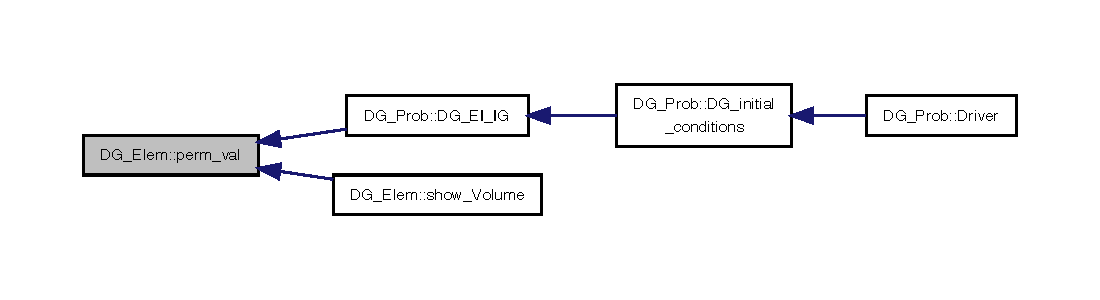
\includegraphics[width=350pt]{classDG__Elem_a699a198b44d02b1394229e623cd6632d_icgraph}
\end{center}
\end{figure}
\mbox{\Hypertarget{classPhElem_aa67e9fd1399ee905803999ef50581677}\label{classPhElem_aa67e9fd1399ee905803999ef50581677}} 
\index{D\+G\+\_\+\+Elem@{D\+G\+\_\+\+Elem}!Phi\+\_\+val@{Phi\+\_\+val}}
\index{Phi\+\_\+val@{Phi\+\_\+val}!D\+G\+\_\+\+Elem@{D\+G\+\_\+\+Elem}}
\subsubsection{\texorpdfstring{Phi\+\_\+val()}{Phi\_val()}}
{\footnotesize\ttfamily double \hyperlink{classPhElem}{Ph\+Elem}$<$ Num\+Variaveis $>$\+::Phi\+\_\+val (\begin{DoxyParamCaption}\item[{const int \&}]{var,  }\item[{const int \&}]{ind,  }\item[{const int \&}]{pos }\end{DoxyParamCaption})\hspace{0.3cm}{\ttfamily [inline]}, {\ttfamily [inherited]}}



Definition at line 140 of file Ph\+Elem.\+hpp.



References Ph\+Elem$<$ Num\+Variaveis $>$\+::anexa\+\_\+gbnmap(), Ph\+Elem$<$ Num\+Variaveis $>$\+::\+Atualizar\+\_\+u0(), Ph\+Elem$<$ Num\+Variaveis $>$\+::\+Avancar\+\_\+u0(), Ph\+Elem$<$ Num\+Variaveis $>$\+::\+Comparar\+\_\+u0(), Ph\+Elem$<$ Num\+Variaveis $>$\+::\+Copia\+\_\+u0\+\_\+em\+\_\+(), Ph\+Elem$<$ Num\+Variaveis $>$\+::escrever\+\_\+restart(), Ph\+Elem$<$ Num\+Variaveis $>$\+::gbnmap\+\_\+aresta(), Ph\+Elem$<$ Num\+Variaveis $>$\+::gbnmap\+\_\+arestas(), Ph\+Elem$<$ Num\+Variaveis $>$\+::gbnmap\+\_\+faces(), Ph\+Elem$<$ Num\+Variaveis $>$\+::gbnmap\+\_\+interior(), Ph\+Elem$<$ Num\+Variaveis $>$\+::gbnmap\+\_\+vertices(), Ph\+Elem$<$ Num\+Variaveis $>$\+::get\+\_\+trace\+\_\+border\+\_\+map(), Ph\+Elem$<$ Num\+Variaveis $>$\+::\+Imprimir\+\_\+valores(), Ph\+Elem$<$ Num\+Variaveis $>$\+::ler\+\_\+restart(), Ph\+Elem$<$ Num\+Variaveis $>$\+::ler\+\_\+restart\+\_\+buffer(), Ph\+Elem$<$ Num\+Variaveis $>$\+::printw\+G\+Q\+J(), Ph\+Elem$<$ Num\+Variaveis $>$\+::projetar\+\_\+\+C0(), Ph\+Elem$<$ Num\+Variaveis $>$\+::ptr\+\_\+stdel, Ph\+Elem$<$ Num\+Variaveis $>$\+::restart\+\_\+element(), Ph\+Elem$<$ Num\+Variaveis $>$\+::\+Restaurar\+\_\+u0(), Ph\+Elem$<$ Num\+Variaveis $>$\+::\+Salvar\+\_\+u0(), Ph\+Elem$<$ Num\+Variaveis $>$\+::set\+\_\+border\+\_\+num(), Ph\+Elem$<$ Num\+Variaveis $>$\+::set\+\_\+border\+\_\+tipo(), Stdel\+::show\+\_\+\+Phi\+\_\+val(), Ph\+Elem$<$ Num\+Variaveis $>$\+::sinal, Ph\+Elem$<$ Num\+Variaveis $>$\+::teste\+\_\+gradiente(), Ph\+Elem$<$ Num\+Variaveis $>$\+::teste\+\_\+transformacao\+\_\+direta(), Ph\+Elem$<$ Num\+Variaveis $>$\+::transformacao\+\_\+direta(), and Ph\+Elem$<$ Num\+Variaveis $>$\+::vetor\+\_\+superficie().

\mbox{\Hypertarget{classPhElem_a233fb1bc0c15cae815fef5d1dc8d9265}\label{classPhElem_a233fb1bc0c15cae815fef5d1dc8d9265}} 
\index{D\+G\+\_\+\+Elem@{D\+G\+\_\+\+Elem}!print\+\_\+matrices@{print\+\_\+matrices}}
\index{print\+\_\+matrices@{print\+\_\+matrices}!D\+G\+\_\+\+Elem@{D\+G\+\_\+\+Elem}}
\subsubsection{\texorpdfstring{print\+\_\+matrices()}{print\_matrices()}}
{\footnotesize\ttfamily void \hyperlink{classPhElem}{Ph\+Elem}$<$ Num\+Variaveis $>$\+::print\+\_\+matrices (\begin{DoxyParamCaption}\item[{F\+I\+LE $\ast$}]{fout }\end{DoxyParamCaption})\hspace{0.3cm}{\ttfamily [inherited]}}

\mbox{\Hypertarget{classPhElem_ae7659320b2118608e38d192443bb2b8f}\label{classPhElem_ae7659320b2118608e38d192443bb2b8f}} 
\index{D\+G\+\_\+\+Elem@{D\+G\+\_\+\+Elem}!print\+\_\+modes@{print\+\_\+modes}}
\index{print\+\_\+modes@{print\+\_\+modes}!D\+G\+\_\+\+Elem@{D\+G\+\_\+\+Elem}}
\subsubsection{\texorpdfstring{print\+\_\+modes()}{print\_modes()}}
{\footnotesize\ttfamily void \hyperlink{classPhElem}{Ph\+Elem}$<$ Num\+Variaveis $>$\+::print\+\_\+modes (\begin{DoxyParamCaption}\item[{F\+I\+LE $\ast$}]{fout,  }\item[{const int \&}]{k }\end{DoxyParamCaption}) const\hspace{0.3cm}{\ttfamily [inherited]}}



Definition at line 551 of file Ph\+Elem.\+hpp.



References Ph\+Elem$<$ Num\+Variaveis $>$\+::gbnmap, Stdel\+::nv\+\_\+val(), and Ph\+Elem$<$ Num\+Variaveis $>$\+::ptr\+\_\+stdel.

\mbox{\Hypertarget{classPhElem_a8d2c46990cba5a5459198d883b763eab}\label{classPhElem_a8d2c46990cba5a5459198d883b763eab}} 
\index{D\+G\+\_\+\+Elem@{D\+G\+\_\+\+Elem}!print\+\_\+numeracao@{print\+\_\+numeracao}}
\index{print\+\_\+numeracao@{print\+\_\+numeracao}!D\+G\+\_\+\+Elem@{D\+G\+\_\+\+Elem}}
\subsubsection{\texorpdfstring{print\+\_\+numeracao()}{print\_numeracao()}}
{\footnotesize\ttfamily void \hyperlink{classPhElem}{Ph\+Elem}$<$ Num\+Variaveis $>$\+::print\+\_\+numeracao (\begin{DoxyParamCaption}\item[{F\+I\+LE $\ast$}]{fout,  }\item[{const int \&}]{k }\end{DoxyParamCaption})\hspace{0.3cm}{\ttfamily [inherited]}}



Definition at line 541 of file Ph\+Elem.\+hpp.



References Ph\+Elem$<$ Num\+Variaveis $>$\+::gbnmap, and Ph\+Elem$<$ Num\+Variaveis $>$\+::numb.

\mbox{\Hypertarget{classPhElem_a53eb1654e889d3fc893f50dcea12adcb}\label{classPhElem_a53eb1654e889d3fc893f50dcea12adcb}} 
\index{D\+G\+\_\+\+Elem@{D\+G\+\_\+\+Elem}!printw\+G\+QJ@{printw\+G\+QJ}}
\index{printw\+G\+QJ@{printw\+G\+QJ}!D\+G\+\_\+\+Elem@{D\+G\+\_\+\+Elem}}
\subsubsection{\texorpdfstring{printw\+G\+Q\+J()}{printwGQJ()}}
{\footnotesize\ttfamily void \hyperlink{classPhElem}{Ph\+Elem}$<$ Num\+Variaveis $>$\+::printw\+G\+QJ (\begin{DoxyParamCaption}\item[{F\+I\+LE $\ast$}]{fileout }\end{DoxyParamCaption})\hspace{0.3cm}{\ttfamily [inherited]}}



Definition at line 316 of file Ph\+Elem.\+hpp.



References Ph\+Elem$<$ Num\+Variaveis $>$\+::\+JV, Stdel\+::printw\+G\+Qtofile(), Ph\+Elem$<$ Num\+Variaveis $>$\+::ptr\+\_\+stdel, Ph\+Elem$<$ Num\+Variaveis $>$\+::ptvert, and Ph\+Elem$<$ Num\+Variaveis $>$\+::\+Vert\+\_\+map.

\mbox{\Hypertarget{classPhElem_a6e4284fcb95240394293c1a576deb738}\label{classPhElem_a6e4284fcb95240394293c1a576deb738}} 
\index{D\+G\+\_\+\+Elem@{D\+G\+\_\+\+Elem}!Processar\+\_\+dados@{Processar\+\_\+dados}}
\index{Processar\+\_\+dados@{Processar\+\_\+dados}!D\+G\+\_\+\+Elem@{D\+G\+\_\+\+Elem}}
\subsubsection{\texorpdfstring{Processar\+\_\+dados()}{Processar\_dados()}}
{\footnotesize\ttfamily void \hyperlink{classPhElem}{Ph\+Elem}$<$ Num\+Variaveis $>$\+::Processar\+\_\+dados (\begin{DoxyParamCaption}\item[{int \&}]{NL,  }\item[{std\+::vector$<$ \hyperlink{structARESTA}{A\+R\+E\+S\+TA} $>$ \&}]{aresta,  }\item[{int \&}]{NF,  }\item[{std\+::vector$<$ \hyperlink{structFACE}{F\+A\+CE} $>$ \&}]{face\+\_\+vec }\end{DoxyParamCaption})\hspace{0.3cm}{\ttfamily [inherited]}}



Definition at line 682 of file Ph\+Elem.\+hpp.



References aresta\+\_\+gbnum(), Stdel\+::aresta\+\_\+lvert(), Ph\+Elem$<$ Num\+Variaveis $>$\+::aresta\+\_\+map, face\+\_\+gbnum(), Stdel\+::face\+\_\+lvert(), Ph\+Elem$<$ Num\+Variaveis $>$\+::face\+\_\+map, n0, Stdel\+::nborder\+\_\+val(), Ph\+Elem$<$ Num\+Variaveis $>$\+::ndim, Stdel\+::ndim\+\_\+val(), Stdel\+::ne\+\_\+val(), Stdel\+::nf\+\_\+val(), Ph\+Elem$<$ Num\+Variaveis $>$\+::numborders, Ph\+Elem$<$ Num\+Variaveis $>$\+::nume, Ph\+Elem$<$ Num\+Variaveis $>$\+::numf, Ph\+Elem$<$ Num\+Variaveis $>$\+::numv, Stdel\+::nv\+\_\+val(), Ph\+Elem$<$ Num\+Variaveis $>$\+::ptr\+\_\+stdel, Stdel\+::show\+\_\+face\+\_\+tipo(), Stdel\+::show\+\_\+nvf(), Ph\+Elem$<$ Num\+Variaveis $>$\+::sinal, and Ph\+Elem$<$ Num\+Variaveis $>$\+::\+Vert\+\_\+map.

\mbox{\Hypertarget{classPhElem_aa5f168531640b2fb9ac82f85e5f8b11a}\label{classPhElem_aa5f168531640b2fb9ac82f85e5f8b11a}} 
\index{D\+G\+\_\+\+Elem@{D\+G\+\_\+\+Elem}!projetar\+\_\+\+C0@{projetar\+\_\+\+C0}}
\index{projetar\+\_\+\+C0@{projetar\+\_\+\+C0}!D\+G\+\_\+\+Elem@{D\+G\+\_\+\+Elem}}
\subsubsection{\texorpdfstring{projetar\+\_\+\+C0()}{projetar\_C0()}}
{\footnotesize\ttfamily void \hyperlink{classPhElem}{Ph\+Elem}$<$ Num\+Variaveis $>$\+::projetar\+\_\+\+C0 (\begin{DoxyParamCaption}\item[{F\+I\+LE $\ast$}]{file,  }\item[{double($\ast$)(double, double, double)}]{func,  }\item[{const int \&}]{ivar }\end{DoxyParamCaption})\hspace{0.3cm}{\ttfamily [inherited]}}



Definition at line 880 of file Ph\+Elem.\+hpp.



References aux, B(), Stdel\+::compute\+Func\+G\+Q(), Stdel\+::\+Dirichlet(), Stdel\+::eval\+\_\+\+Phi(), Ph\+Elem$<$ Num\+Variaveis $>$\+::\+JV, Stdel\+::mass(), Stdel\+::\+N\+G\+Q\+P\+\_\+val(), Ph\+Elem$<$ Num\+Variaveis $>$\+::numb, Ph\+Elem$<$ Num\+Variaveis $>$\+::numborders, Ph\+Elem$<$ Num\+Variaveis $>$\+::numn, Stdel\+::printtofile(), Ph\+Elem$<$ Num\+Variaveis $>$\+::ptr\+\_\+stdel, Ph\+Elem$<$ Num\+Variaveis $>$\+::ptvert, Ph\+Elem$<$ Num\+Variaveis $>$\+::sgn, Ph\+Elem$<$ Num\+Variaveis $>$\+::u0, Stdel\+::vector\+\_\+of\+\_\+integral\+\_\+of\+\_\+f\+\_\+\+Phi\+\_\+dv(), and Ph\+Elem$<$ Num\+Variaveis $>$\+::\+Vert\+\_\+map.

\mbox{\Hypertarget{classPhElem_a8abc7be8120f4192de31e0cfb32ac968}\label{classPhElem_a8abc7be8120f4192de31e0cfb32ac968}} 
\index{D\+G\+\_\+\+Elem@{D\+G\+\_\+\+Elem}!read\+\_\+vertices@{read\+\_\+vertices}}
\index{read\+\_\+vertices@{read\+\_\+vertices}!D\+G\+\_\+\+Elem@{D\+G\+\_\+\+Elem}}
\subsubsection{\texorpdfstring{read\+\_\+vertices()}{read\_vertices()}}
{\footnotesize\ttfamily void \hyperlink{classPhElem}{Ph\+Elem}$<$ Num\+Variaveis $>$\+::read\+\_\+vertices (\begin{DoxyParamCaption}\item[{F\+I\+LE $\ast$}]{finput,  }\item[{const int \&}]{nv }\end{DoxyParamCaption})\hspace{0.3cm}{\ttfamily [inherited]}}



Definition at line 563 of file Ph\+Elem.\+hpp.



References Ph\+Elem$<$ Num\+Variaveis $>$\+::\+Vert\+\_\+map.

\mbox{\Hypertarget{classPhElem_abe273d496e748985021a8f67ef598c0d}\label{classPhElem_abe273d496e748985021a8f67ef598c0d}} 
\index{D\+G\+\_\+\+Elem@{D\+G\+\_\+\+Elem}!restart\+\_\+element@{restart\+\_\+element}}
\index{restart\+\_\+element@{restart\+\_\+element}!D\+G\+\_\+\+Elem@{D\+G\+\_\+\+Elem}}
\subsubsection{\texorpdfstring{restart\+\_\+element()}{restart\_element()}}
{\footnotesize\ttfamily void \hyperlink{classPhElem}{Ph\+Elem}$<$ Num\+Variaveis $>$\+::restart\+\_\+element (\begin{DoxyParamCaption}\item[{double $\ast$}]{buff,  }\item[{int \&}]{count }\end{DoxyParamCaption})\hspace{0.3cm}{\ttfamily [inherited]}}



Definition at line 270 of file Ph\+Elem.\+hpp.



References Ph\+Elem$<$ Num\+Variaveis $>$\+::numn, and Ph\+Elem$<$ Num\+Variaveis $>$\+::u0.

\mbox{\Hypertarget{classPhElem_a7094a0e8767868c583cc948e56214a9d}\label{classPhElem_a7094a0e8767868c583cc948e56214a9d}} 
\index{D\+G\+\_\+\+Elem@{D\+G\+\_\+\+Elem}!Restaurar\+\_\+u0@{Restaurar\+\_\+u0}}
\index{Restaurar\+\_\+u0@{Restaurar\+\_\+u0}!D\+G\+\_\+\+Elem@{D\+G\+\_\+\+Elem}}
\subsubsection{\texorpdfstring{Restaurar\+\_\+u0()}{Restaurar\_u0()}}
{\footnotesize\ttfamily void \hyperlink{classPhElem}{Ph\+Elem}$<$ Num\+Variaveis $>$\+::Restaurar\+\_\+u0 (\begin{DoxyParamCaption}{ }\end{DoxyParamCaption})\hspace{0.3cm}{\ttfamily [inherited]}}



Definition at line 333 of file Ph\+Elem.\+hpp.



References Ph\+Elem$<$ Num\+Variaveis $>$\+::numn, Ph\+Elem$<$ Num\+Variaveis $>$\+::u0, and Ph\+Elem$<$ Num\+Variaveis $>$\+::usave.

\mbox{\Hypertarget{classPhElem_ab6765ea1fa41b3a2d565d86872d6e7e6}\label{classPhElem_ab6765ea1fa41b3a2d565d86872d6e7e6}} 
\index{D\+G\+\_\+\+Elem@{D\+G\+\_\+\+Elem}!Salvar\+\_\+u0@{Salvar\+\_\+u0}}
\index{Salvar\+\_\+u0@{Salvar\+\_\+u0}!D\+G\+\_\+\+Elem@{D\+G\+\_\+\+Elem}}
\subsubsection{\texorpdfstring{Salvar\+\_\+u0()}{Salvar\_u0()}}
{\footnotesize\ttfamily void \hyperlink{classPhElem}{Ph\+Elem}$<$ Num\+Variaveis $>$\+::Salvar\+\_\+u0 (\begin{DoxyParamCaption}{ }\end{DoxyParamCaption})\hspace{0.3cm}{\ttfamily [inherited]}}



Definition at line 325 of file Ph\+Elem.\+hpp.



References Ph\+Elem$<$ Num\+Variaveis $>$\+::numn, Ph\+Elem$<$ Num\+Variaveis $>$\+::u0, and Ph\+Elem$<$ Num\+Variaveis $>$\+::usave.

\mbox{\Hypertarget{classPhElem_a05b05802884ecd42ed42e46108a0d5b1}\label{classPhElem_a05b05802884ecd42ed42e46108a0d5b1}} 
\index{D\+G\+\_\+\+Elem@{D\+G\+\_\+\+Elem}!set\+\_\+border\+\_\+num@{set\+\_\+border\+\_\+num}}
\index{set\+\_\+border\+\_\+num@{set\+\_\+border\+\_\+num}!D\+G\+\_\+\+Elem@{D\+G\+\_\+\+Elem}}
\subsubsection{\texorpdfstring{set\+\_\+border\+\_\+num()}{set\_border\_num()}}
{\footnotesize\ttfamily void \hyperlink{classPhElem}{Ph\+Elem}$<$ Num\+Variaveis $>$\+::set\+\_\+border\+\_\+num (\begin{DoxyParamCaption}\item[{const int \&}]{aresta,  }\item[{const int \&}]{num }\end{DoxyParamCaption})\hspace{0.3cm}{\ttfamily [inherited]}}



Definition at line 514 of file Ph\+Elem.\+hpp.



References Ph\+Elem$<$ Num\+Variaveis $>$\+::border\+\_\+num.

\mbox{\Hypertarget{classPhElem_aafd112d676dc3e16309e8ec8980f1c97}\label{classPhElem_aafd112d676dc3e16309e8ec8980f1c97}} 
\index{D\+G\+\_\+\+Elem@{D\+G\+\_\+\+Elem}!set\+\_\+border\+\_\+tipo@{set\+\_\+border\+\_\+tipo}}
\index{set\+\_\+border\+\_\+tipo@{set\+\_\+border\+\_\+tipo}!D\+G\+\_\+\+Elem@{D\+G\+\_\+\+Elem}}
\subsubsection{\texorpdfstring{set\+\_\+border\+\_\+tipo()}{set\_border\_tipo()}}
{\footnotesize\ttfamily void \hyperlink{classPhElem}{Ph\+Elem}$<$ Num\+Variaveis $>$\+::set\+\_\+border\+\_\+tipo (\begin{DoxyParamCaption}\item[{\hyperlink{structEDGE}{E\+D\+GE} $\ast$}]{border,  }\item[{const int \&}]{aresta,  }\item[{const int \&}]{t }\end{DoxyParamCaption})\hspace{0.3cm}{\ttfamily [inherited]}}



Definition at line 503 of file Ph\+Elem.\+hpp.



References Ph\+Elem$<$ Num\+Variaveis $>$\+::border\+\_\+num, and E\+D\+G\+E\+::tipo.

\mbox{\Hypertarget{classDG__Elem_a9f7165dbb388e11f16b4249383f71d0e}\label{classDG__Elem_a9f7165dbb388e11f16b4249383f71d0e}} 
\index{D\+G\+\_\+\+Elem@{D\+G\+\_\+\+Elem}!set\+\_\+fontes@{set\+\_\+fontes}}
\index{set\+\_\+fontes@{set\+\_\+fontes}!D\+G\+\_\+\+Elem@{D\+G\+\_\+\+Elem}}
\subsubsection{\texorpdfstring{set\+\_\+fontes()}{set\_fontes()}}
{\footnotesize\ttfamily void D\+G\+\_\+\+Elem\+::set\+\_\+fontes (\begin{DoxyParamCaption}\item[{double}]{sw,  }\item[{double}]{sn }\end{DoxyParamCaption})\hspace{0.3cm}{\ttfamily [inline]}}



Definition at line 27 of file D\+G\+\_\+\+Elem.\+hpp.



References qn, qw, and sn.



Referenced by D\+G\+\_\+\+Prob\+::\+D\+G\+\_\+initial\+\_\+conditions(), and D\+G\+\_\+\+Prob\+::projetar\+\_\+\+C0().

Here is the caller graph for this function\+:
\nopagebreak
\begin{figure}[H]
\begin{center}
\leavevmode
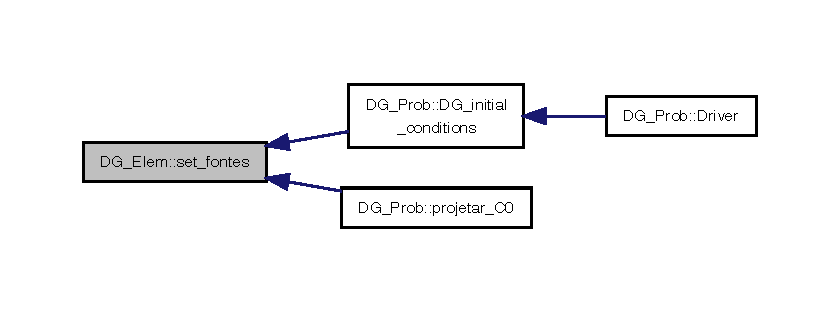
\includegraphics[width=350pt]{classDG__Elem_a9f7165dbb388e11f16b4249383f71d0e_icgraph}
\end{center}
\end{figure}
\mbox{\Hypertarget{classPhElem_afba886f63bf7b67bd0a4164eae4dde5b}\label{classPhElem_afba886f63bf7b67bd0a4164eae4dde5b}} 
\index{D\+G\+\_\+\+Elem@{D\+G\+\_\+\+Elem}!set\+\_\+gbnmap@{set\+\_\+gbnmap}}
\index{set\+\_\+gbnmap@{set\+\_\+gbnmap}!D\+G\+\_\+\+Elem@{D\+G\+\_\+\+Elem}}
\subsubsection{\texorpdfstring{set\+\_\+gbnmap()}{set\_gbnmap()}}
{\footnotesize\ttfamily void \hyperlink{classPhElem}{Ph\+Elem}$<$ Num\+Variaveis $>$\+::set\+\_\+gbnmap (\begin{DoxyParamCaption}\item[{const int \&}]{ia,  }\item[{const int}]{gbnmap\+\_\+temp\mbox{[}$\,$\mbox{]},  }\item[{const int}]{sgn\+\_\+temp\mbox{[}$\,$\mbox{]} }\end{DoxyParamCaption})\hspace{0.3cm}{\ttfamily [inherited]}}



Definition at line 789 of file Ph\+Elem.\+hpp.



References Ph\+Elem$<$ Num\+Variaveis $>$\+::gbnmap, Ph\+Elem$<$ Num\+Variaveis $>$\+::numn, and Ph\+Elem$<$ Num\+Variaveis $>$\+::sgn.

\mbox{\Hypertarget{classDG__Elem_a132e9ad800e701395b1e21d291040ff2}\label{classDG__Elem_a132e9ad800e701395b1e21d291040ff2}} 
\index{D\+G\+\_\+\+Elem@{D\+G\+\_\+\+Elem}!set\+\_\+mass\+\_\+density@{set\+\_\+mass\+\_\+density}}
\index{set\+\_\+mass\+\_\+density@{set\+\_\+mass\+\_\+density}!D\+G\+\_\+\+Elem@{D\+G\+\_\+\+Elem}}
\subsubsection{\texorpdfstring{set\+\_\+mass\+\_\+density()}{set\_mass\_density()}}
{\footnotesize\ttfamily void D\+G\+\_\+\+Elem\+::set\+\_\+mass\+\_\+density (\begin{DoxyParamCaption}\item[{double}]{value }\end{DoxyParamCaption})}



Definition at line 38 of file D\+G\+\_\+\+Elem.\+cpp.



References rho.



Referenced by show\+\_\+\+Volume().

Here is the caller graph for this function\+:
\nopagebreak
\begin{figure}[H]
\begin{center}
\leavevmode
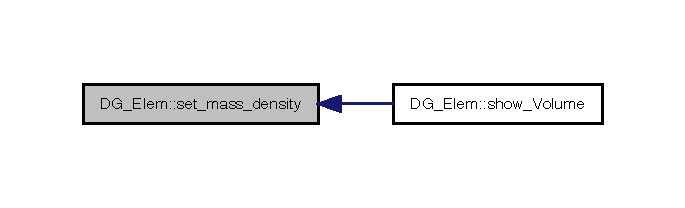
\includegraphics[width=329pt]{classDG__Elem_a132e9ad800e701395b1e21d291040ff2_icgraph}
\end{center}
\end{figure}
\mbox{\Hypertarget{classPhElem_a24a705e62f179fa36c6886f8f0a3ef25}\label{classPhElem_a24a705e62f179fa36c6886f8f0a3ef25}} 
\index{D\+G\+\_\+\+Elem@{D\+G\+\_\+\+Elem}!set\+\_\+part\+\_\+num@{set\+\_\+part\+\_\+num}}
\index{set\+\_\+part\+\_\+num@{set\+\_\+part\+\_\+num}!D\+G\+\_\+\+Elem@{D\+G\+\_\+\+Elem}}
\subsubsection{\texorpdfstring{set\+\_\+part\+\_\+num()}{set\_part\_num()}}
{\footnotesize\ttfamily void \hyperlink{classPhElem}{Ph\+Elem}$<$ Num\+Variaveis $>$\+::set\+\_\+part\+\_\+num (\begin{DoxyParamCaption}\item[{const int \&}]{num = {\ttfamily -\/1} }\end{DoxyParamCaption})\hspace{0.3cm}{\ttfamily [inherited]}}



Definition at line 1406 of file Ph\+Elem.\+hpp.



References Ph\+Elem$<$ Num\+Variaveis $>$\+::numv, Vertice\+::part\+\_\+num, Ph\+Elem$<$ Num\+Variaveis $>$\+::part\+\_\+num, Ph\+Elem$<$ Num\+Variaveis $>$\+::ptvert, and Ph\+Elem$<$ Num\+Variaveis $>$\+::\+Vert\+\_\+map.

\mbox{\Hypertarget{classDG__Elem_a51393e54786059782e6a0502f00cdd50}\label{classDG__Elem_a51393e54786059782e6a0502f00cdd50}} 
\index{D\+G\+\_\+\+Elem@{D\+G\+\_\+\+Elem}!set\+\_\+permeabilidade@{set\+\_\+permeabilidade}}
\index{set\+\_\+permeabilidade@{set\+\_\+permeabilidade}!D\+G\+\_\+\+Elem@{D\+G\+\_\+\+Elem}}
\subsubsection{\texorpdfstring{set\+\_\+permeabilidade()}{set\_permeabilidade()}}
{\footnotesize\ttfamily void D\+G\+\_\+\+Elem\+::set\+\_\+permeabilidade (\begin{DoxyParamCaption}\item[{const double}]{x,  }\item[{const double}]{y,  }\item[{const double}]{z }\end{DoxyParamCaption})}



Definition at line 30 of file D\+G\+\_\+\+Elem.\+cpp.



References perm.



Referenced by D\+G\+\_\+\+Prob\+::\+D\+G\+\_\+initial\+\_\+conditions(), D\+G\+\_\+\+Prob\+::projetar\+\_\+\+C0(), and show\+\_\+\+Volume().

Here is the caller graph for this function\+:
\nopagebreak
\begin{figure}[H]
\begin{center}
\leavevmode
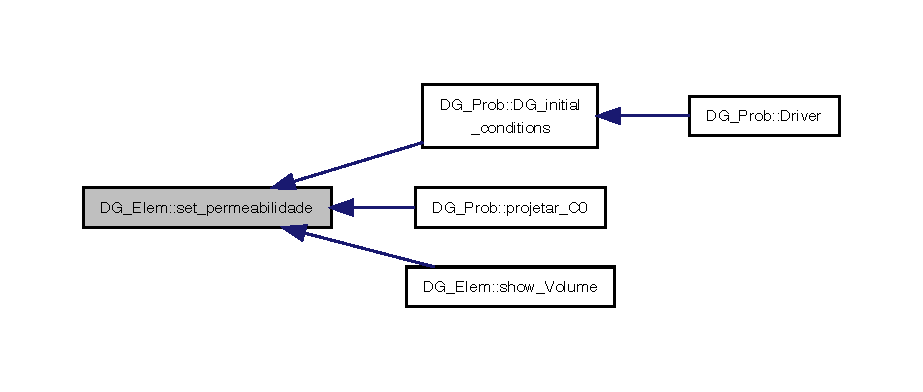
\includegraphics[width=350pt]{classDG__Elem_a51393e54786059782e6a0502f00cdd50_icgraph}
\end{center}
\end{figure}
\mbox{\Hypertarget{classDG__Elem_a5d8512886cb22395c92265f5eee6a940}\label{classDG__Elem_a5d8512886cb22395c92265f5eee6a940}} 
\index{D\+G\+\_\+\+Elem@{D\+G\+\_\+\+Elem}!set\+\_\+porosidade@{set\+\_\+porosidade}}
\index{set\+\_\+porosidade@{set\+\_\+porosidade}!D\+G\+\_\+\+Elem@{D\+G\+\_\+\+Elem}}
\subsubsection{\texorpdfstring{set\+\_\+porosidade()}{set\_porosidade()}}
{\footnotesize\ttfamily void D\+G\+\_\+\+Elem\+::set\+\_\+porosidade (\begin{DoxyParamCaption}\item[{double}]{value }\end{DoxyParamCaption})}



Definition at line 152 of file D\+G\+\_\+\+Elem.\+cpp.



References porosidade.



Referenced by D\+G\+\_\+\+Prob\+::\+D\+G\+\_\+initial\+\_\+conditions(), D\+G\+\_\+\+Prob\+::projetar\+\_\+\+C0(), and show\+\_\+\+Volume().

Here is the caller graph for this function\+:
\nopagebreak
\begin{figure}[H]
\begin{center}
\leavevmode
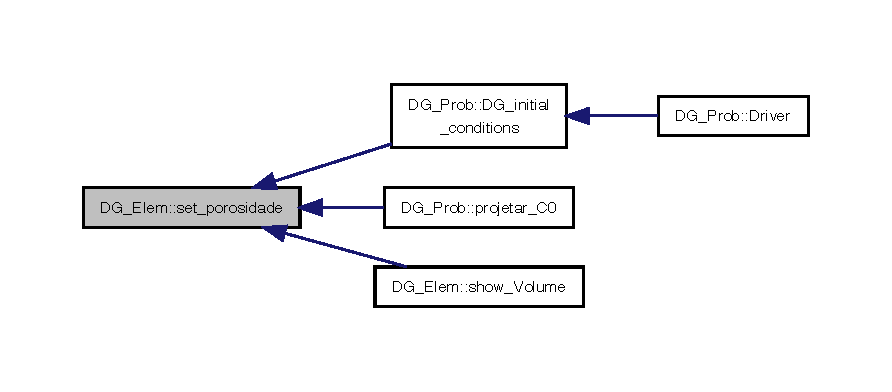
\includegraphics[width=350pt]{classDG__Elem_a5d8512886cb22395c92265f5eee6a940_icgraph}
\end{center}
\end{figure}
\mbox{\Hypertarget{classPhElem_af2796c868709214bb9b151b47d7d471f}\label{classPhElem_af2796c868709214bb9b151b47d7d471f}} 
\index{D\+G\+\_\+\+Elem@{D\+G\+\_\+\+Elem}!set\+\_\+ptr\+\_\+stdel@{set\+\_\+ptr\+\_\+stdel}}
\index{set\+\_\+ptr\+\_\+stdel@{set\+\_\+ptr\+\_\+stdel}!D\+G\+\_\+\+Elem@{D\+G\+\_\+\+Elem}}
\subsubsection{\texorpdfstring{set\+\_\+ptr\+\_\+stdel()}{set\_ptr\_stdel()}\hspace{0.1cm}{\footnotesize\ttfamily [1/3]}}
{\footnotesize\ttfamily void \hyperlink{classPhElem}{Ph\+Elem}$<$ Num\+Variaveis $>$\+::set\+\_\+ptr\+\_\+stdel (\begin{DoxyParamCaption}\item[{\hyperlink{classStdel}{Stdel} $\ast$}]{pointer,  }\item[{\hyperlink{classStdel}{Stdel} $\ast$}]{pointer1 }\end{DoxyParamCaption})\hspace{0.3cm}{\ttfamily [inherited]}}



Definition at line 460 of file Ph\+Elem.\+hpp.



References Stdel\+::nb\+\_\+val(), Stdel\+::nn\+\_\+val(), Ph\+Elem$<$ Num\+Variaveis $>$\+::numb, Ph\+Elem$<$ Num\+Variaveis $>$\+::numn, and Ph\+Elem$<$ Num\+Variaveis $>$\+::ptr\+\_\+stdel.

\mbox{\Hypertarget{classPhElem_aaf841c14455a54e0f33e2c74bef979fd}\label{classPhElem_aaf841c14455a54e0f33e2c74bef979fd}} 
\index{D\+G\+\_\+\+Elem@{D\+G\+\_\+\+Elem}!set\+\_\+ptr\+\_\+stdel@{set\+\_\+ptr\+\_\+stdel}}
\index{set\+\_\+ptr\+\_\+stdel@{set\+\_\+ptr\+\_\+stdel}!D\+G\+\_\+\+Elem@{D\+G\+\_\+\+Elem}}
\subsubsection{\texorpdfstring{set\+\_\+ptr\+\_\+stdel()}{set\_ptr\_stdel()}\hspace{0.1cm}{\footnotesize\ttfamily [2/3]}}
{\footnotesize\ttfamily void \hyperlink{classPhElem}{Ph\+Elem}$<$ Num\+Variaveis $>$\+::set\+\_\+ptr\+\_\+stdel (\begin{DoxyParamCaption}\item[{\hyperlink{classStdel}{Stdel} $\ast$}]{pointers\mbox{[}$\,$\mbox{]} }\end{DoxyParamCaption})\hspace{0.3cm}{\ttfamily [inherited]}}



Definition at line 482 of file Ph\+Elem.\+hpp.



References Stdel\+::nb\+\_\+val(), Stdel\+::nn\+\_\+val(), Ph\+Elem$<$ Num\+Variaveis $>$\+::numb, Ph\+Elem$<$ Num\+Variaveis $>$\+::numn, and Ph\+Elem$<$ Num\+Variaveis $>$\+::ptr\+\_\+stdel.

\mbox{\Hypertarget{classPhElem_a78130ee8d7d6ecf59f231dbd436e9081}\label{classPhElem_a78130ee8d7d6ecf59f231dbd436e9081}} 
\index{D\+G\+\_\+\+Elem@{D\+G\+\_\+\+Elem}!set\+\_\+ptr\+\_\+stdel@{set\+\_\+ptr\+\_\+stdel}}
\index{set\+\_\+ptr\+\_\+stdel@{set\+\_\+ptr\+\_\+stdel}!D\+G\+\_\+\+Elem@{D\+G\+\_\+\+Elem}}
\subsubsection{\texorpdfstring{set\+\_\+ptr\+\_\+stdel()}{set\_ptr\_stdel()}\hspace{0.1cm}{\footnotesize\ttfamily [3/3]}}
{\footnotesize\ttfamily void \hyperlink{classPhElem}{Ph\+Elem}$<$ Num\+Variaveis $>$\+::set\+\_\+ptr\+\_\+stdel (\begin{DoxyParamCaption}\item[{\hyperlink{classStdel}{Stdel} $\ast$}]{pointer }\end{DoxyParamCaption})\hspace{0.3cm}{\ttfamily [inherited]}}



Definition at line 452 of file Ph\+Elem.\+hpp.



References Stdel\+::nb\+\_\+val(), Stdel\+::nn\+\_\+val(), Ph\+Elem$<$ Num\+Variaveis $>$\+::numb, Ph\+Elem$<$ Num\+Variaveis $>$\+::numn, and Ph\+Elem$<$ Num\+Variaveis $>$\+::ptr\+\_\+stdel.

\mbox{\Hypertarget{classPhElem_a52fdbcf2283aacd8fdf9672018d74e4a}\label{classPhElem_a52fdbcf2283aacd8fdf9672018d74e4a}} 
\index{D\+G\+\_\+\+Elem@{D\+G\+\_\+\+Elem}!set\+\_\+ptr\+\_\+stdel\+\_\+var@{set\+\_\+ptr\+\_\+stdel\+\_\+var}}
\index{set\+\_\+ptr\+\_\+stdel\+\_\+var@{set\+\_\+ptr\+\_\+stdel\+\_\+var}!D\+G\+\_\+\+Elem@{D\+G\+\_\+\+Elem}}
\subsubsection{\texorpdfstring{set\+\_\+ptr\+\_\+stdel\+\_\+var()}{set\_ptr\_stdel\_var()}}
{\footnotesize\ttfamily void \hyperlink{classPhElem}{Ph\+Elem}$<$ Num\+Variaveis $>$\+::set\+\_\+ptr\+\_\+stdel\+\_\+var (\begin{DoxyParamCaption}\item[{const int}]{ind,  }\item[{\hyperlink{classStdel}{Stdel} $\ast$}]{pointer }\end{DoxyParamCaption})\hspace{0.3cm}{\ttfamily [inherited]}}



Definition at line 474 of file Ph\+Elem.\+hpp.



References Stdel\+::nb\+\_\+val(), Stdel\+::nn\+\_\+val(), Ph\+Elem$<$ Num\+Variaveis $>$\+::numb, Ph\+Elem$<$ Num\+Variaveis $>$\+::numn, and Ph\+Elem$<$ Num\+Variaveis $>$\+::ptr\+\_\+stdel.

\mbox{\Hypertarget{classPhElem_a8ed472a9e135b1e16b962c14df8f2225}\label{classPhElem_a8ed472a9e135b1e16b962c14df8f2225}} 
\index{D\+G\+\_\+\+Elem@{D\+G\+\_\+\+Elem}!set\+\_\+ptvert@{set\+\_\+ptvert}}
\index{set\+\_\+ptvert@{set\+\_\+ptvert}!D\+G\+\_\+\+Elem@{D\+G\+\_\+\+Elem}}
\subsubsection{\texorpdfstring{set\+\_\+ptvert()}{set\_ptvert()}}
{\footnotesize\ttfamily void \hyperlink{classPhElem}{Ph\+Elem}$<$ Num\+Variaveis $>$\+::set\+\_\+ptvert (\begin{DoxyParamCaption}\item[{const \hyperlink{structVertice}{Vertice} $\ast$}]{pointer }\end{DoxyParamCaption})\hspace{0.3cm}{\ttfamily [inherited]}}



Definition at line 493 of file Ph\+Elem.\+hpp.



References Ph\+Elem$<$ Num\+Variaveis $>$\+::ptvert.

\mbox{\Hypertarget{classPhElem_a03505c861fbcdb7cf8faec9fe5eea088}\label{classPhElem_a03505c861fbcdb7cf8faec9fe5eea088}} 
\index{D\+G\+\_\+\+Elem@{D\+G\+\_\+\+Elem}!set\+\_\+sgn@{set\+\_\+sgn}}
\index{set\+\_\+sgn@{set\+\_\+sgn}!D\+G\+\_\+\+Elem@{D\+G\+\_\+\+Elem}}
\subsubsection{\texorpdfstring{set\+\_\+sgn()}{set\_sgn()}}
{\footnotesize\ttfamily void \hyperlink{classPhElem}{Ph\+Elem}$<$ Num\+Variaveis $>$\+::set\+\_\+sgn (\begin{DoxyParamCaption}{ }\end{DoxyParamCaption})\hspace{0.3cm}{\ttfamily [inherited]}}

\mbox{\Hypertarget{classPhElem_ae63196241e8f39617acb1984cb06910e}\label{classPhElem_ae63196241e8f39617acb1984cb06910e}} 
\index{D\+G\+\_\+\+Elem@{D\+G\+\_\+\+Elem}!set\+\_\+stgbtrbmap@{set\+\_\+stgbtrbmap}}
\index{set\+\_\+stgbtrbmap@{set\+\_\+stgbtrbmap}!D\+G\+\_\+\+Elem@{D\+G\+\_\+\+Elem}}
\subsubsection{\texorpdfstring{set\+\_\+stgbtrbmap()}{set\_stgbtrbmap()}}
{\footnotesize\ttfamily void \hyperlink{classPhElem}{Ph\+Elem}$<$ Num\+Variaveis $>$\+::set\+\_\+stgbtrbmap (\begin{DoxyParamCaption}\item[{const int \&}]{b,  }\item[{const int \&}]{vmapM,  }\item[{const int \&}]{vmapP }\end{DoxyParamCaption})\hspace{0.3cm}{\ttfamily [inherited]}}



Definition at line 870 of file Ph\+Elem.\+hpp.



References Ph\+Elem$<$ Num\+Variaveis $>$\+::stgbtrbmapM, and Ph\+Elem$<$ Num\+Variaveis $>$\+::stgbtrbmapP.

\mbox{\Hypertarget{classPhElem_ae226a41912e8e7c76be365518b2a38e2}\label{classPhElem_ae226a41912e8e7c76be365518b2a38e2}} 
\index{D\+G\+\_\+\+Elem@{D\+G\+\_\+\+Elem}!set\+\_\+type@{set\+\_\+type}}
\index{set\+\_\+type@{set\+\_\+type}!D\+G\+\_\+\+Elem@{D\+G\+\_\+\+Elem}}
\subsubsection{\texorpdfstring{set\+\_\+type()}{set\_type()}}
{\footnotesize\ttfamily void \hyperlink{classPhElem}{Ph\+Elem}$<$ Num\+Variaveis $>$\+::set\+\_\+type (\begin{DoxyParamCaption}\item[{const int \&}]{num }\end{DoxyParamCaption})\hspace{0.3cm}{\ttfamily [inherited]}}



Definition at line 529 of file Ph\+Elem.\+hpp.



References Ph\+Elem$<$ Num\+Variaveis $>$\+::type.

\mbox{\Hypertarget{classPhElem_a134cbfd28fc238a24156ab1c24fc31c0}\label{classPhElem_a134cbfd28fc238a24156ab1c24fc31c0}} 
\index{D\+G\+\_\+\+Elem@{D\+G\+\_\+\+Elem}!set\+\_\+\+Vert\+\_\+map@{set\+\_\+\+Vert\+\_\+map}}
\index{set\+\_\+\+Vert\+\_\+map@{set\+\_\+\+Vert\+\_\+map}!D\+G\+\_\+\+Elem@{D\+G\+\_\+\+Elem}}
\subsubsection{\texorpdfstring{set\+\_\+\+Vert\+\_\+map()}{set\_Vert\_map()}}
{\footnotesize\ttfamily void \hyperlink{classPhElem}{Ph\+Elem}$<$ Num\+Variaveis $>$\+::set\+\_\+\+Vert\+\_\+map (\begin{DoxyParamCaption}\item[{const int \&}]{n\+\_\+in,  }\item[{int}]{ver\+\_\+temp\mbox{[}$\,$\mbox{]} }\end{DoxyParamCaption})\hspace{0.3cm}{\ttfamily [inherited]}}



Definition at line 774 of file Ph\+Elem.\+hpp.



References Ph\+Elem$<$ Num\+Variaveis $>$\+::numv, Ph\+Elem$<$ Num\+Variaveis $>$\+::type, and Ph\+Elem$<$ Num\+Variaveis $>$\+::\+Vert\+\_\+map.

\mbox{\Hypertarget{classPhElem_ac6f5e03dd6e155037363dbd0ea2f401b}\label{classPhElem_ac6f5e03dd6e155037363dbd0ea2f401b}} 
\index{D\+G\+\_\+\+Elem@{D\+G\+\_\+\+Elem}!show\+\_\+\+Aresta@{show\+\_\+\+Aresta}}
\index{show\+\_\+\+Aresta@{show\+\_\+\+Aresta}!D\+G\+\_\+\+Elem@{D\+G\+\_\+\+Elem}}
\subsubsection{\texorpdfstring{show\+\_\+\+Aresta()}{show\_Aresta()}}
{\footnotesize\ttfamily int \hyperlink{classPhElem}{Ph\+Elem}$<$ Num\+Variaveis $>$\+::show\+\_\+\+Aresta (\begin{DoxyParamCaption}\item[{int}]{i }\end{DoxyParamCaption})\hspace{0.3cm}{\ttfamily [inline]}, {\ttfamily [inherited]}}



Definition at line 133 of file Ph\+Elem.\+hpp.



References Ph\+Elem$<$ Num\+Variaveis $>$\+::aresta\+\_\+map.

\mbox{\Hypertarget{classPhElem_a0caf55d9fac7477102ee34373c67a024}\label{classPhElem_a0caf55d9fac7477102ee34373c67a024}} 
\index{D\+G\+\_\+\+Elem@{D\+G\+\_\+\+Elem}!show\+\_\+b0@{show\+\_\+b0}}
\index{show\+\_\+b0@{show\+\_\+b0}!D\+G\+\_\+\+Elem@{D\+G\+\_\+\+Elem}}
\subsubsection{\texorpdfstring{show\+\_\+b0()}{show\_b0()}\hspace{0.1cm}{\footnotesize\ttfamily [1/2]}}
{\footnotesize\ttfamily double \hyperlink{classPhElem}{Ph\+Elem}$<$ Num\+Variaveis $>$\+::show\+\_\+b0 (\begin{DoxyParamCaption}\item[{const int \&}]{i }\end{DoxyParamCaption})\hspace{0.3cm}{\ttfamily [inherited]}}

\mbox{\Hypertarget{classPhElem_afb4171c67795f5614d9628d59f3bfaf7}\label{classPhElem_afb4171c67795f5614d9628d59f3bfaf7}} 
\index{D\+G\+\_\+\+Elem@{D\+G\+\_\+\+Elem}!show\+\_\+b0@{show\+\_\+b0}}
\index{show\+\_\+b0@{show\+\_\+b0}!D\+G\+\_\+\+Elem@{D\+G\+\_\+\+Elem}}
\subsubsection{\texorpdfstring{show\+\_\+b0()}{show\_b0()}\hspace{0.1cm}{\footnotesize\ttfamily [2/2]}}
{\footnotesize\ttfamily double \hyperlink{classPhElem}{Ph\+Elem}$<$ Num\+Variaveis $>$\+::show\+\_\+b0 (\begin{DoxyParamCaption}\item[{const int \&}]{var,  }\item[{const int \&}]{no }\end{DoxyParamCaption})\hspace{0.3cm}{\ttfamily [inherited]}}



Definition at line 602 of file Ph\+Elem.\+hpp.



References Ph\+Elem$<$ Num\+Variaveis $>$\+::b0.

\mbox{\Hypertarget{classPhElem_a13564919b6d9747f0e6b33f3e8aae31b}\label{classPhElem_a13564919b6d9747f0e6b33f3e8aae31b}} 
\index{D\+G\+\_\+\+Elem@{D\+G\+\_\+\+Elem}!show\+\_\+border\+\_\+num@{show\+\_\+border\+\_\+num}}
\index{show\+\_\+border\+\_\+num@{show\+\_\+border\+\_\+num}!D\+G\+\_\+\+Elem@{D\+G\+\_\+\+Elem}}
\subsubsection{\texorpdfstring{show\+\_\+border\+\_\+num()}{show\_border\_num()}}
{\footnotesize\ttfamily int \hyperlink{classPhElem}{Ph\+Elem}$<$ Num\+Variaveis $>$\+::show\+\_\+border\+\_\+num (\begin{DoxyParamCaption}\item[{int}]{i }\end{DoxyParamCaption})\hspace{0.3cm}{\ttfamily [inline]}, {\ttfamily [inherited]}}



Definition at line 136 of file Ph\+Elem.\+hpp.



References Ph\+Elem$<$ Num\+Variaveis $>$\+::border\+\_\+num.

\mbox{\Hypertarget{classPhElem_a0846ec2cbd31a24aea440c29a71d50ec}\label{classPhElem_a0846ec2cbd31a24aea440c29a71d50ec}} 
\index{D\+G\+\_\+\+Elem@{D\+G\+\_\+\+Elem}!show\+\_\+bs@{show\+\_\+bs}}
\index{show\+\_\+bs@{show\+\_\+bs}!D\+G\+\_\+\+Elem@{D\+G\+\_\+\+Elem}}
\subsubsection{\texorpdfstring{show\+\_\+bs()}{show\_bs()}}
{\footnotesize\ttfamily double \hyperlink{classPhElem}{Ph\+Elem}$<$ Num\+Variaveis $>$\+::show\+\_\+bs (\begin{DoxyParamCaption}\item[{const int \&}]{var,  }\item[{const int \&}]{no }\end{DoxyParamCaption})\hspace{0.3cm}{\ttfamily [inherited]}}



Definition at line 609 of file Ph\+Elem.\+hpp.



References Ph\+Elem$<$ Num\+Variaveis $>$\+::bs.

\mbox{\Hypertarget{classPhElem_a916c6927d0964574d815a13dd80f1e30}\label{classPhElem_a916c6927d0964574d815a13dd80f1e30}} 
\index{D\+G\+\_\+\+Elem@{D\+G\+\_\+\+Elem}!show\+\_\+\+Face@{show\+\_\+\+Face}}
\index{show\+\_\+\+Face@{show\+\_\+\+Face}!D\+G\+\_\+\+Elem@{D\+G\+\_\+\+Elem}}
\subsubsection{\texorpdfstring{show\+\_\+\+Face()}{show\_Face()}}
{\footnotesize\ttfamily int \hyperlink{classPhElem}{Ph\+Elem}$<$ Num\+Variaveis $>$\+::show\+\_\+\+Face (\begin{DoxyParamCaption}\item[{int}]{i }\end{DoxyParamCaption})\hspace{0.3cm}{\ttfamily [inline]}, {\ttfamily [inherited]}}



Definition at line 134 of file Ph\+Elem.\+hpp.



References Ph\+Elem$<$ Num\+Variaveis $>$\+::face\+\_\+map.

\mbox{\Hypertarget{classPhElem_a878851914f553298700437c5c8aef4dd}\label{classPhElem_a878851914f553298700437c5c8aef4dd}} 
\index{D\+G\+\_\+\+Elem@{D\+G\+\_\+\+Elem}!show\+\_\+gbnmap@{show\+\_\+gbnmap}}
\index{show\+\_\+gbnmap@{show\+\_\+gbnmap}!D\+G\+\_\+\+Elem@{D\+G\+\_\+\+Elem}}
\subsubsection{\texorpdfstring{show\+\_\+gbnmap()}{show\_gbnmap()}}
{\footnotesize\ttfamily const int \hyperlink{classPhElem}{Ph\+Elem}$<$ Num\+Variaveis $>$\+::show\+\_\+gbnmap (\begin{DoxyParamCaption}\item[{int}]{ivar,  }\item[{int}]{modo }\end{DoxyParamCaption}) const\hspace{0.3cm}{\ttfamily [inline]}, {\ttfamily [inherited]}}



Definition at line 39 of file Ph\+Elem.\+hpp.



References Ph\+Elem$<$ Num\+Variaveis $>$\+::gbnmap.

\mbox{\Hypertarget{classPhElem_a2addc4d79151aeac865e2255be3b417d}\label{classPhElem_a2addc4d79151aeac865e2255be3b417d}} 
\index{D\+G\+\_\+\+Elem@{D\+G\+\_\+\+Elem}!show\+\_\+gbtrbmap@{show\+\_\+gbtrbmap}}
\index{show\+\_\+gbtrbmap@{show\+\_\+gbtrbmap}!D\+G\+\_\+\+Elem@{D\+G\+\_\+\+Elem}}
\subsubsection{\texorpdfstring{show\+\_\+gbtrbmap()}{show\_gbtrbmap()}}
{\footnotesize\ttfamily int \hyperlink{classPhElem}{Ph\+Elem}$<$ Num\+Variaveis $>$\+::show\+\_\+gbtrbmap (\begin{DoxyParamCaption}{ }\end{DoxyParamCaption})\hspace{0.3cm}{\ttfamily [inline]}, {\ttfamily [inherited]}}



Definition at line 105 of file Ph\+Elem.\+hpp.



References Ph\+Elem$<$ Num\+Variaveis $>$\+::gbtrbmap.

\mbox{\Hypertarget{classPhElem_a63b2f67b4f782432909cd7d32d188996}\label{classPhElem_a63b2f67b4f782432909cd7d32d188996}} 
\index{D\+G\+\_\+\+Elem@{D\+G\+\_\+\+Elem}!show\+\_\+J@{show\+\_\+J}}
\index{show\+\_\+J@{show\+\_\+J}!D\+G\+\_\+\+Elem@{D\+G\+\_\+\+Elem}}
\subsubsection{\texorpdfstring{show\+\_\+\+J()}{show\_J()}}
{\footnotesize\ttfamily double \hyperlink{classPhElem}{Ph\+Elem}$<$ Num\+Variaveis $>$\+::show\+\_\+J (\begin{DoxyParamCaption}{ }\end{DoxyParamCaption})\hspace{0.3cm}{\ttfamily [inline]}, {\ttfamily [inherited]}}



Definition at line 129 of file Ph\+Elem.\+hpp.



References Ph\+Elem$<$ Num\+Variaveis $>$\+::J, and Ph\+Elem$<$ Num\+Variaveis $>$\+::make\+\_\+\+Mass\+Matrices().

\mbox{\Hypertarget{classPhElem_aca4ef303cd316714d116062e8f4d8ca5}\label{classPhElem_aca4ef303cd316714d116062e8f4d8ca5}} 
\index{D\+G\+\_\+\+Elem@{D\+G\+\_\+\+Elem}!show\+\_\+nume@{show\+\_\+nume}}
\index{show\+\_\+nume@{show\+\_\+nume}!D\+G\+\_\+\+Elem@{D\+G\+\_\+\+Elem}}
\subsubsection{\texorpdfstring{show\+\_\+nume()}{show\_nume()}}
{\footnotesize\ttfamily int \hyperlink{classPhElem}{Ph\+Elem}$<$ Num\+Variaveis $>$\+::show\+\_\+nume (\begin{DoxyParamCaption}{ }\end{DoxyParamCaption})\hspace{0.3cm}{\ttfamily [inline]}, {\ttfamily [inherited]}}



Definition at line 41 of file Ph\+Elem.\+hpp.



References Ph\+Elem$<$ Num\+Variaveis $>$\+::nume.

\mbox{\Hypertarget{classPhElem_afbe63a88e47733c8daec89a4c72b7da0}\label{classPhElem_afbe63a88e47733c8daec89a4c72b7da0}} 
\index{D\+G\+\_\+\+Elem@{D\+G\+\_\+\+Elem}!show\+\_\+numf@{show\+\_\+numf}}
\index{show\+\_\+numf@{show\+\_\+numf}!D\+G\+\_\+\+Elem@{D\+G\+\_\+\+Elem}}
\subsubsection{\texorpdfstring{show\+\_\+numf()}{show\_numf()}}
{\footnotesize\ttfamily int \hyperlink{classPhElem}{Ph\+Elem}$<$ Num\+Variaveis $>$\+::show\+\_\+numf (\begin{DoxyParamCaption}{ }\end{DoxyParamCaption})\hspace{0.3cm}{\ttfamily [inline]}, {\ttfamily [inherited]}}



Definition at line 42 of file Ph\+Elem.\+hpp.



References a, Ph\+Elem$<$ Num\+Variaveis $>$\+::assign\+\_\+gbnmap(), Ph\+Elem$<$ Num\+Variaveis $>$\+::check\+\_\+connectivity(), Ph\+Elem$<$ Num\+Variaveis $>$\+::compute\+\_\+\+J\+V(), Ph\+Elem$<$ Num\+Variaveis $>$\+::\+Increment\+\_\+field(), Ph\+Elem$<$ Num\+Variaveis $>$\+::inicia\+\_\+gbnmap(), Ph\+Elem$<$ Num\+Variaveis $>$\+::inicia\+\_\+gbtrbmap(), Ph\+Elem$<$ Num\+Variaveis $>$\+::\+K\+\_\+\+Imisc2\+F(), Ph\+Elem$<$ Num\+Variaveis $>$\+::\+Kcomp(), Ph\+Elem$<$ Num\+Variaveis $>$\+::make\+\_\+\+K\+\_\+\+Elast2\+D(), Ph\+Elem$<$ Num\+Variaveis $>$\+::make\+\_\+\+K\+\_\+\+Imiscivel2\+F(), Ph\+Elem$<$ Num\+Variaveis $>$\+::make\+\_\+\+Kcomp\+\_\+\+Elast2\+D(), Ph\+Elem$<$ Num\+Variaveis $>$\+::make\+\_\+\+Kcomp\+\_\+\+Elast2\+D\+\_\+dyn(), Ph\+Elem$<$ Num\+Variaveis $>$\+::make\+\_\+vector(), Ph\+Elem$<$ Num\+Variaveis $>$\+::make\+\_\+vector\+\_\+\+Elast2\+D\+\_\+dyn(), Ph\+Elem$<$ Num\+Variaveis $>$\+::make\+\_\+\+Vector\+\_\+\+Eq\+\_\+\+S1(), Ph\+Elem$<$ Num\+Variaveis $>$\+::map(), Ph\+Elem$<$ Num\+Variaveis $>$\+::mapa\+\_\+inverso(), Ph\+Elem$<$ Num\+Variaveis $>$\+::numf, Ph\+Elem$<$ Num\+Variaveis $>$\+::\+P\+\_\+eval\+\_\+phys(), Ph\+Elem$<$ Num\+Variaveis $>$\+::\+P\+\_\+eval\+\_\+print(), Ph\+Elem$<$ Num\+Variaveis $>$\+::\+P\+\_\+eval\+\_\+print\+\_\+\+Elast2\+D(), Ph\+Elem$<$ Num\+Variaveis $>$\+::\+P\+\_\+eval\+\_\+print\+\_\+\+Elast2\+D\+\_\+dyn(), Ph\+Elem$<$ Num\+Variaveis $>$\+::\+P\+\_\+eval\+\_\+u(), Ph\+Elem$<$ Num\+Variaveis $>$\+::\+P\+\_\+eval\+\_\+u\+\_\+p1(), Ph\+Elem$<$ Num\+Variaveis $>$\+::\+P\+\_\+eval\+\_\+vert(), Ph\+Elem$<$ Num\+Variaveis $>$\+::\+P\+\_\+print(), Ph\+Elem$<$ Num\+Variaveis $>$\+::print\+\_\+matrices(), Ph\+Elem$<$ Num\+Variaveis $>$\+::print\+\_\+modes(), Ph\+Elem$<$ Num\+Variaveis $>$\+::print\+\_\+numeracao(), Ph\+Elem$<$ Num\+Variaveis $>$\+::\+Processar\+\_\+dados(), Ph\+Elem$<$ Num\+Variaveis $>$\+::set\+\_\+gbnmap(), Ph\+Elem$<$ Num\+Variaveis $>$\+::set\+\_\+stgbtrbmap(), Ph\+Elem$<$ Num\+Variaveis $>$\+::set\+\_\+type(), Ph\+Elem$<$ Num\+Variaveis $>$\+::type\+\_\+val(), Ph\+Elem$<$ Num\+Variaveis $>$\+::\+Vector\+Elast2\+D(), Ph\+Elem$<$ Num\+Variaveis $>$\+::zera\+\_\+bs(), and Ph\+Elem$<$ Num\+Variaveis $>$\+::zera\+\_\+vetores().

\mbox{\Hypertarget{classPhElem_a5288b2eba55ffa37f1a9866a516f6886}\label{classPhElem_a5288b2eba55ffa37f1a9866a516f6886}} 
\index{D\+G\+\_\+\+Elem@{D\+G\+\_\+\+Elem}!show\+\_\+\+Num\+Local\+Vars@{show\+\_\+\+Num\+Local\+Vars}}
\index{show\+\_\+\+Num\+Local\+Vars@{show\+\_\+\+Num\+Local\+Vars}!D\+G\+\_\+\+Elem@{D\+G\+\_\+\+Elem}}
\subsubsection{\texorpdfstring{show\+\_\+\+Num\+Local\+Vars()}{show\_NumLocalVars()}}
{\footnotesize\ttfamily int \hyperlink{classPhElem}{Ph\+Elem}$<$ Num\+Variaveis $>$\+::show\+\_\+\+Num\+Local\+Vars (\begin{DoxyParamCaption}{ }\end{DoxyParamCaption})\hspace{0.3cm}{\ttfamily [inline]}, {\ttfamily [inherited]}}



Definition at line 28 of file Ph\+Elem.\+hpp.



References Ph\+Elem$<$ Num\+Variaveis $>$\+::\+Num\+Local\+Vars, Ph\+Elem$<$ Num\+Variaveis $>$\+::read\+\_\+vertices(), Ph\+Elem$<$ Num\+Variaveis $>$\+::set\+\_\+ptr\+\_\+stdel(), Ph\+Elem$<$ Num\+Variaveis $>$\+::set\+\_\+ptr\+\_\+stdel\+\_\+var(), Ph\+Elem$<$ Num\+Variaveis $>$\+::set\+\_\+ptvert(), Ph\+Elem$<$ Num\+Variaveis $>$\+::set\+\_\+sgn(), Ph\+Elem$<$ Num\+Variaveis $>$\+::set\+\_\+\+Vert\+\_\+map(), and Ph\+Elem$<$ Num\+Variaveis $>$\+::teste().

\mbox{\Hypertarget{classPhElem_a69a5cfc5b3b7faa4ad5f584311406ce1}\label{classPhElem_a69a5cfc5b3b7faa4ad5f584311406ce1}} 
\index{D\+G\+\_\+\+Elem@{D\+G\+\_\+\+Elem}!show\+\_\+numv@{show\+\_\+numv}}
\index{show\+\_\+numv@{show\+\_\+numv}!D\+G\+\_\+\+Elem@{D\+G\+\_\+\+Elem}}
\subsubsection{\texorpdfstring{show\+\_\+numv()}{show\_numv()}}
{\footnotesize\ttfamily int \hyperlink{classPhElem}{Ph\+Elem}$<$ Num\+Variaveis $>$\+::show\+\_\+numv (\begin{DoxyParamCaption}{ }\end{DoxyParamCaption})\hspace{0.3cm}{\ttfamily [inline]}, {\ttfamily [inherited]}}



Definition at line 40 of file Ph\+Elem.\+hpp.



References Ph\+Elem$<$ Num\+Variaveis $>$\+::numv.

\mbox{\Hypertarget{classPhElem_a7a476e9682accd03064f3e8bec39fb50}\label{classPhElem_a7a476e9682accd03064f3e8bec39fb50}} 
\index{D\+G\+\_\+\+Elem@{D\+G\+\_\+\+Elem}!show\+\_\+part\+\_\+num@{show\+\_\+part\+\_\+num}}
\index{show\+\_\+part\+\_\+num@{show\+\_\+part\+\_\+num}!D\+G\+\_\+\+Elem@{D\+G\+\_\+\+Elem}}
\subsubsection{\texorpdfstring{show\+\_\+part\+\_\+num()}{show\_part\_num()}}
{\footnotesize\ttfamily int \hyperlink{classPhElem}{Ph\+Elem}$<$ Num\+Variaveis $>$\+::show\+\_\+part\+\_\+num (\begin{DoxyParamCaption}{ }\end{DoxyParamCaption})\hspace{0.3cm}{\ttfamily [inline]}, {\ttfamily [inherited]}}



Definition at line 137 of file Ph\+Elem.\+hpp.



References Ph\+Elem$<$ Num\+Variaveis $>$\+::part\+\_\+num, and Ph\+Elem$<$ Num\+Variaveis $>$\+::set\+\_\+part\+\_\+num().

\mbox{\Hypertarget{classPhElem_a227c31195c6832f8e36f8d507806bd54}\label{classPhElem_a227c31195c6832f8e36f8d507806bd54}} 
\index{D\+G\+\_\+\+Elem@{D\+G\+\_\+\+Elem}!show\+\_\+ptr\+\_\+stdel@{show\+\_\+ptr\+\_\+stdel}}
\index{show\+\_\+ptr\+\_\+stdel@{show\+\_\+ptr\+\_\+stdel}!D\+G\+\_\+\+Elem@{D\+G\+\_\+\+Elem}}
\subsubsection{\texorpdfstring{show\+\_\+ptr\+\_\+stdel()}{show\_ptr\_stdel()}}
{\footnotesize\ttfamily \hyperlink{classStdel}{Stdel} $\ast$ \hyperlink{classPhElem}{Ph\+Elem}$<$ Num\+Variaveis $>$\+::show\+\_\+ptr\+\_\+stdel (\begin{DoxyParamCaption}\item[{const int \&}]{n }\end{DoxyParamCaption}) const\hspace{0.3cm}{\ttfamily [inherited]}}



Definition at line 588 of file Ph\+Elem.\+hpp.



References Ph\+Elem$<$ Num\+Variaveis $>$\+::ptr\+\_\+stdel.

\mbox{\Hypertarget{classDG__Elem_acc7285f0df1d6a4544405169daf2853c}\label{classDG__Elem_acc7285f0df1d6a4544405169daf2853c}} 
\index{D\+G\+\_\+\+Elem@{D\+G\+\_\+\+Elem}!show\+\_\+rho@{show\+\_\+rho}}
\index{show\+\_\+rho@{show\+\_\+rho}!D\+G\+\_\+\+Elem@{D\+G\+\_\+\+Elem}}
\subsubsection{\texorpdfstring{show\+\_\+rho()}{show\_rho()}}
{\footnotesize\ttfamily double D\+G\+\_\+\+Elem\+::show\+\_\+rho (\begin{DoxyParamCaption}{ }\end{DoxyParamCaption})\hspace{0.3cm}{\ttfamily [inline]}}



Definition at line 28 of file D\+G\+\_\+\+Elem.\+hpp.



References rho.

\mbox{\Hypertarget{classPhElem_ab271550e1373e11cb0b1f62d3e1ea428}\label{classPhElem_ab271550e1373e11cb0b1f62d3e1ea428}} 
\index{D\+G\+\_\+\+Elem@{D\+G\+\_\+\+Elem}!show\+\_\+sgn@{show\+\_\+sgn}}
\index{show\+\_\+sgn@{show\+\_\+sgn}!D\+G\+\_\+\+Elem@{D\+G\+\_\+\+Elem}}
\subsubsection{\texorpdfstring{show\+\_\+sgn()}{show\_sgn()}}
{\footnotesize\ttfamily int \hyperlink{classPhElem}{Ph\+Elem}$<$ Num\+Variaveis $>$\+::show\+\_\+sgn (\begin{DoxyParamCaption}\item[{const int \&}]{ia,  }\item[{const int \&}]{i }\end{DoxyParamCaption})\hspace{0.3cm}{\ttfamily [inline]}, {\ttfamily [inherited]}}



Definition at line 38 of file Ph\+Elem.\+hpp.



References Ph\+Elem$<$ Num\+Variaveis $>$\+::sgn.

\mbox{\Hypertarget{classPhElem_a47dc705efd50a4484bf407bce4a5e010}\label{classPhElem_a47dc705efd50a4484bf407bce4a5e010}} 
\index{D\+G\+\_\+\+Elem@{D\+G\+\_\+\+Elem}!show\+\_\+sinal@{show\+\_\+sinal}}
\index{show\+\_\+sinal@{show\+\_\+sinal}!D\+G\+\_\+\+Elem@{D\+G\+\_\+\+Elem}}
\subsubsection{\texorpdfstring{show\+\_\+sinal()}{show\_sinal()}}
{\footnotesize\ttfamily int \hyperlink{classPhElem}{Ph\+Elem}$<$ Num\+Variaveis $>$\+::show\+\_\+sinal (\begin{DoxyParamCaption}\item[{int}]{i }\end{DoxyParamCaption})\hspace{0.3cm}{\ttfamily [inline]}, {\ttfamily [inherited]}}



Definition at line 135 of file Ph\+Elem.\+hpp.



References Ph\+Elem$<$ Num\+Variaveis $>$\+::sinal.

\mbox{\Hypertarget{classPhElem_a5f0e8811ea30343e51e4be9ff40d2b74}\label{classPhElem_a5f0e8811ea30343e51e4be9ff40d2b74}} 
\index{D\+G\+\_\+\+Elem@{D\+G\+\_\+\+Elem}!show\+\_\+stgbtrbmapM@{show\+\_\+stgbtrbmapM}}
\index{show\+\_\+stgbtrbmapM@{show\+\_\+stgbtrbmapM}!D\+G\+\_\+\+Elem@{D\+G\+\_\+\+Elem}}
\subsubsection{\texorpdfstring{show\+\_\+stgbtrbmap\+M()}{show\_stgbtrbmapM()}}
{\footnotesize\ttfamily int \hyperlink{classPhElem}{Ph\+Elem}$<$ Num\+Variaveis $>$\+::show\+\_\+stgbtrbmapM (\begin{DoxyParamCaption}\item[{const int \&}]{a }\end{DoxyParamCaption})\hspace{0.3cm}{\ttfamily [inline]}, {\ttfamily [inherited]}}



Definition at line 106 of file Ph\+Elem.\+hpp.



References Ph\+Elem$<$ Num\+Variaveis $>$\+::stgbtrbmapM.

\mbox{\Hypertarget{classPhElem_a3d9e8990f4442e3b17e1cce3c9af19e9}\label{classPhElem_a3d9e8990f4442e3b17e1cce3c9af19e9}} 
\index{D\+G\+\_\+\+Elem@{D\+G\+\_\+\+Elem}!show\+\_\+stgbtrbmapP@{show\+\_\+stgbtrbmapP}}
\index{show\+\_\+stgbtrbmapP@{show\+\_\+stgbtrbmapP}!D\+G\+\_\+\+Elem@{D\+G\+\_\+\+Elem}}
\subsubsection{\texorpdfstring{show\+\_\+stgbtrbmap\+P()}{show\_stgbtrbmapP()}}
{\footnotesize\ttfamily int \hyperlink{classPhElem}{Ph\+Elem}$<$ Num\+Variaveis $>$\+::show\+\_\+stgbtrbmapP (\begin{DoxyParamCaption}\item[{const int \&}]{a }\end{DoxyParamCaption})\hspace{0.3cm}{\ttfamily [inline]}, {\ttfamily [inherited]}}



Definition at line 107 of file Ph\+Elem.\+hpp.



References Ph\+Elem$<$ Num\+Variaveis $>$\+::\+Bound\+Cond(), Ph\+Elem$<$ Num\+Variaveis $>$\+::check\+\_\+gradiente(), Ph\+Elem$<$ Num\+Variaveis $>$\+::\+Neumann(), Ph\+Elem$<$ Num\+Variaveis $>$\+::show\+\_\+b0(), Ph\+Elem$<$ Num\+Variaveis $>$\+::show\+\_\+bs(), Ph\+Elem$<$ Num\+Variaveis $>$\+::show\+\_\+ptr\+\_\+stdel(), Ph\+Elem$<$ Num\+Variaveis $>$\+::show\+\_\+u(), and Ph\+Elem$<$ Num\+Variaveis $>$\+::stgbtrbmapP.

\mbox{\Hypertarget{classPhElem_a27e7bc9ed0ea64d609d4d0b29baba468}\label{classPhElem_a27e7bc9ed0ea64d609d4d0b29baba468}} 
\index{D\+G\+\_\+\+Elem@{D\+G\+\_\+\+Elem}!show\+\_\+u@{show\+\_\+u}}
\index{show\+\_\+u@{show\+\_\+u}!D\+G\+\_\+\+Elem@{D\+G\+\_\+\+Elem}}
\subsubsection{\texorpdfstring{show\+\_\+u()}{show\_u()}\hspace{0.1cm}{\footnotesize\ttfamily [1/2]}}
{\footnotesize\ttfamily double \hyperlink{classPhElem}{Ph\+Elem}$<$ Num\+Variaveis $>$\+::show\+\_\+u (\begin{DoxyParamCaption}\item[{const int \&}]{i }\end{DoxyParamCaption})\hspace{0.3cm}{\ttfamily [inherited]}}

\mbox{\Hypertarget{classPhElem_a9d2b7b826289ccd180fdd4b45d0d7333}\label{classPhElem_a9d2b7b826289ccd180fdd4b45d0d7333}} 
\index{D\+G\+\_\+\+Elem@{D\+G\+\_\+\+Elem}!show\+\_\+u@{show\+\_\+u}}
\index{show\+\_\+u@{show\+\_\+u}!D\+G\+\_\+\+Elem@{D\+G\+\_\+\+Elem}}
\subsubsection{\texorpdfstring{show\+\_\+u()}{show\_u()}\hspace{0.1cm}{\footnotesize\ttfamily [2/2]}}
{\footnotesize\ttfamily double \hyperlink{classPhElem}{Ph\+Elem}$<$ Num\+Variaveis $>$\+::show\+\_\+u (\begin{DoxyParamCaption}\item[{const int \&}]{var,  }\item[{const int \&}]{no }\end{DoxyParamCaption})\hspace{0.3cm}{\ttfamily [inherited]}}



Definition at line 595 of file Ph\+Elem.\+hpp.



References Ph\+Elem$<$ Num\+Variaveis $>$\+::u0.

\mbox{\Hypertarget{classPhElem_ace7e4ec0fa3ca3e829cd790375ab981e}\label{classPhElem_ace7e4ec0fa3ca3e829cd790375ab981e}} 
\index{D\+G\+\_\+\+Elem@{D\+G\+\_\+\+Elem}!show\+\_\+\+Vert\+\_\+map@{show\+\_\+\+Vert\+\_\+map}}
\index{show\+\_\+\+Vert\+\_\+map@{show\+\_\+\+Vert\+\_\+map}!D\+G\+\_\+\+Elem@{D\+G\+\_\+\+Elem}}
\subsubsection{\texorpdfstring{show\+\_\+\+Vert\+\_\+map()}{show\_Vert\_map()}}
{\footnotesize\ttfamily int \hyperlink{classPhElem}{Ph\+Elem}$<$ Num\+Variaveis $>$\+::show\+\_\+\+Vert\+\_\+map (\begin{DoxyParamCaption}\item[{int}]{i }\end{DoxyParamCaption})\hspace{0.3cm}{\ttfamily [inline]}, {\ttfamily [inherited]}}



Definition at line 132 of file Ph\+Elem.\+hpp.



References Ph\+Elem$<$ Num\+Variaveis $>$\+::\+Vert\+\_\+map.

\mbox{\Hypertarget{classDG__Elem_a01a49e07fd18a74e12eedf15cff7b8c7}\label{classDG__Elem_a01a49e07fd18a74e12eedf15cff7b8c7}} 
\index{D\+G\+\_\+\+Elem@{D\+G\+\_\+\+Elem}!show\+\_\+\+Volume@{show\+\_\+\+Volume}}
\index{show\+\_\+\+Volume@{show\+\_\+\+Volume}!D\+G\+\_\+\+Elem@{D\+G\+\_\+\+Elem}}
\subsubsection{\texorpdfstring{show\+\_\+\+Volume()}{show\_Volume()}}
{\footnotesize\ttfamily double D\+G\+\_\+\+Elem\+::show\+\_\+\+Volume (\begin{DoxyParamCaption}{ }\end{DoxyParamCaption})\hspace{0.3cm}{\ttfamily [inline]}}



Definition at line 29 of file D\+G\+\_\+\+Elem.\+hpp.



References Atualizar\+\_\+valores(), B(), calcula\+\_\+tracos(), echo\+\_\+traco(), finaliza\+\_\+vetores(), inicia\+\_\+funcoes\+\_\+na\+\_\+borda(), inicia\+\_\+tracos(), perm\+\_\+val(), set\+\_\+mass\+\_\+density(), set\+\_\+permeabilidade(), set\+\_\+porosidade(), Traco\+\_\+\+Kgrad\+\_\+pc(), Traco\+\_\+\+Kgrad\+\_\+pw(), Traco\+\_\+\+Kgrad\+\_\+sn(), Traco\+\_\+phi(), Traco\+\_\+pw(), Traco\+\_\+sn(), Volume, Volume\+Integrals(), Volume\+Integrals\+\_\+\+I\+G(), Volume\+Integrals\+\_\+\+U\+M\+F\+P\+A\+C\+K(), Volume\+Integrals\+T(), and Volume\+Tracos().

Here is the call graph for this function\+:
\nopagebreak
\begin{figure}[H]
\begin{center}
\leavevmode
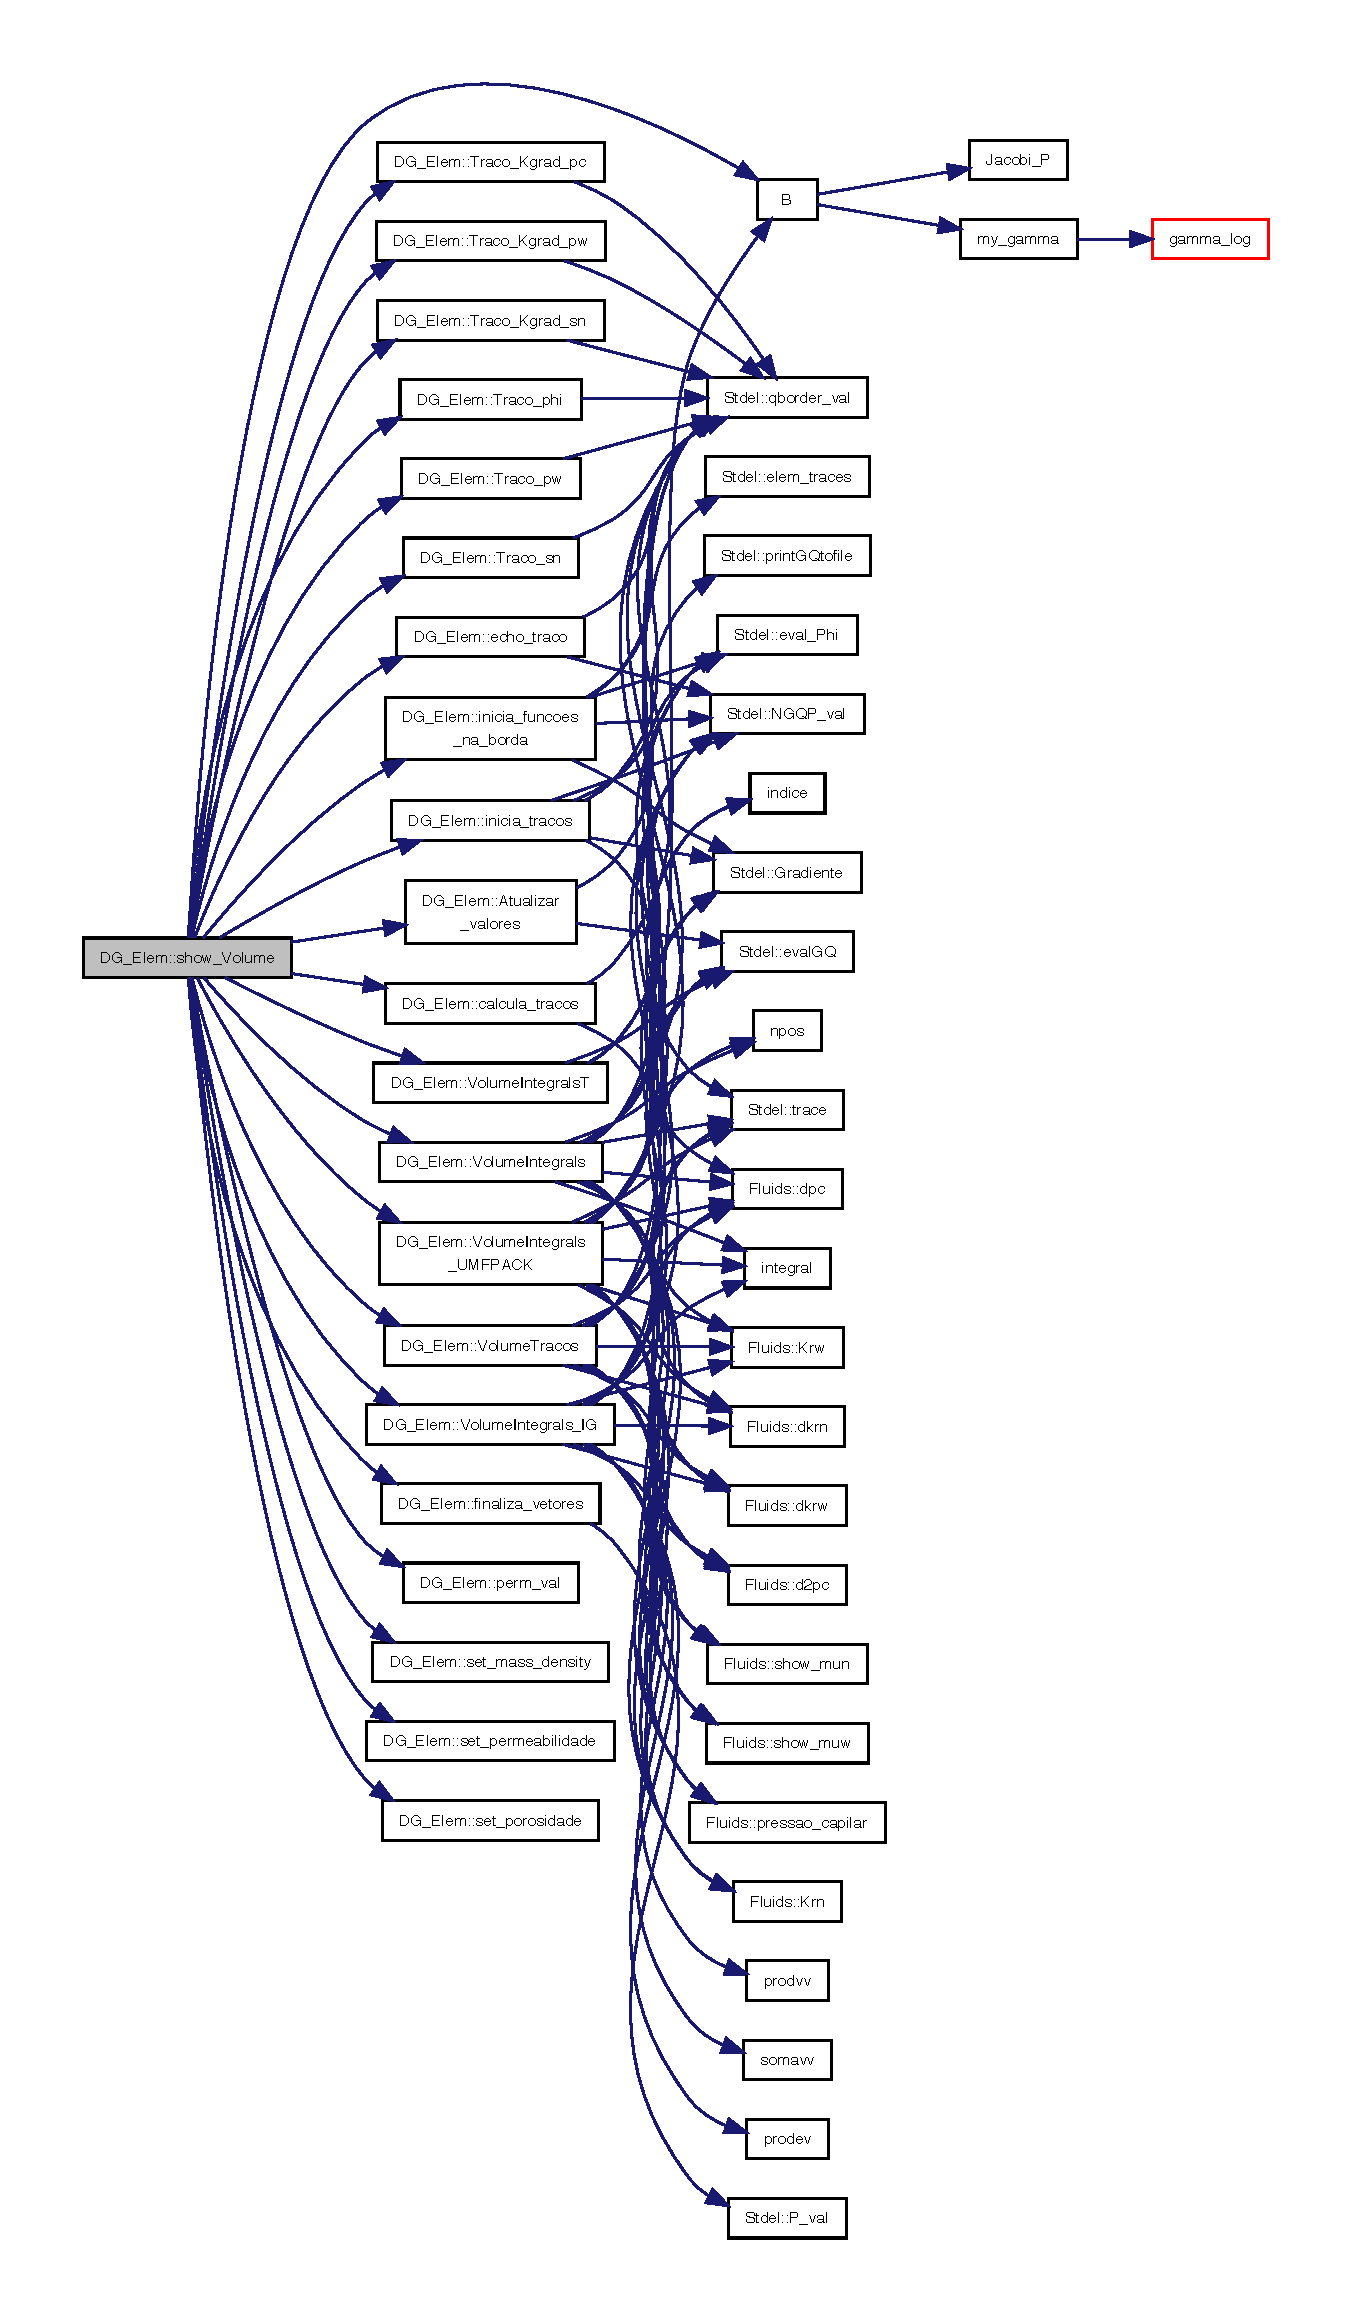
\includegraphics[height=550pt]{classDG__Elem_a01a49e07fd18a74e12eedf15cff7b8c7_cgraph}
\end{center}
\end{figure}
\mbox{\Hypertarget{classPhElem_a9742fa2313cf25a24ae9c5602bd75ac0}\label{classPhElem_a9742fa2313cf25a24ae9c5602bd75ac0}} 
\index{D\+G\+\_\+\+Elem@{D\+G\+\_\+\+Elem}!teste@{teste}}
\index{teste@{teste}!D\+G\+\_\+\+Elem@{D\+G\+\_\+\+Elem}}
\subsubsection{\texorpdfstring{teste()}{teste()}}
{\footnotesize\ttfamily void \hyperlink{classPhElem}{Ph\+Elem}$<$ Num\+Variaveis $>$\+::teste (\begin{DoxyParamCaption}{ }\end{DoxyParamCaption})\hspace{0.3cm}{\ttfamily [inherited]}}



Definition at line 189 of file Elastostatica.\+cpp.

\mbox{\Hypertarget{classPhElem_adc3411d8b3a88f04004b6d48e64e9334}\label{classPhElem_adc3411d8b3a88f04004b6d48e64e9334}} 
\index{D\+G\+\_\+\+Elem@{D\+G\+\_\+\+Elem}!teste\+\_\+gradiente@{teste\+\_\+gradiente}}
\index{teste\+\_\+gradiente@{teste\+\_\+gradiente}!D\+G\+\_\+\+Elem@{D\+G\+\_\+\+Elem}}
\subsubsection{\texorpdfstring{teste\+\_\+gradiente()}{teste\_gradiente()}}
{\footnotesize\ttfamily void \hyperlink{classPhElem}{Ph\+Elem}$<$ Num\+Variaveis $>$\+::teste\+\_\+gradiente (\begin{DoxyParamCaption}{ }\end{DoxyParamCaption})\hspace{0.3cm}{\ttfamily [inherited]}}



Definition at line 1426 of file Ph\+Elem.\+hpp.



References aux, e, Stdel\+::eval\+\_\+\+Grad\+Phi(), Stdel\+::eval\+\_\+\+Phi(), Stdel\+::\+Gradiente(), Ph\+Elem$<$ Num\+Variaveis $>$\+::ndim, Stdel\+::\+N\+G\+Q\+P\+\_\+val(), Ph\+Elem$<$ Num\+Variaveis $>$\+::numn, Ph\+Elem$<$ Num\+Variaveis $>$\+::ptr\+\_\+stdel, Ph\+Elem$<$ Num\+Variaveis $>$\+::ptvert, and Ph\+Elem$<$ Num\+Variaveis $>$\+::\+Vert\+\_\+map.

\mbox{\Hypertarget{classPhElem_a68e2ff863aa38d90933fc033e1fcec0e}\label{classPhElem_a68e2ff863aa38d90933fc033e1fcec0e}} 
\index{D\+G\+\_\+\+Elem@{D\+G\+\_\+\+Elem}!teste\+\_\+transformacao\+\_\+direta@{teste\+\_\+transformacao\+\_\+direta}}
\index{teste\+\_\+transformacao\+\_\+direta@{teste\+\_\+transformacao\+\_\+direta}!D\+G\+\_\+\+Elem@{D\+G\+\_\+\+Elem}}
\subsubsection{\texorpdfstring{teste\+\_\+transformacao\+\_\+direta()}{teste\_transformacao\_direta()}}
{\footnotesize\ttfamily void \hyperlink{classPhElem}{Ph\+Elem}$<$ Num\+Variaveis $>$\+::teste\+\_\+transformacao\+\_\+direta (\begin{DoxyParamCaption}\item[{F\+I\+LE $\ast$}]{fin,  }\item[{F\+I\+LE $\ast$}]{fout,  }\item[{const int \&}]{npoints,  }\item[{const double}]{coord\mbox{[}$\,$\mbox{]} }\end{DoxyParamCaption})\hspace{0.3cm}{\ttfamily [inherited]}}

\mbox{\Hypertarget{classDG__Elem_a8d090e18204cd99ed11ef8115a95c2e7}\label{classDG__Elem_a8d090e18204cd99ed11ef8115a95c2e7}} 
\index{D\+G\+\_\+\+Elem@{D\+G\+\_\+\+Elem}!Traco\+\_\+grad\+\_\+phi@{Traco\+\_\+grad\+\_\+phi}}
\index{Traco\+\_\+grad\+\_\+phi@{Traco\+\_\+grad\+\_\+phi}!D\+G\+\_\+\+Elem@{D\+G\+\_\+\+Elem}}
\subsubsection{\texorpdfstring{Traco\+\_\+grad\+\_\+phi()}{Traco\_grad\_phi()}}
{\footnotesize\ttfamily void D\+G\+\_\+\+Elem\+::\+Traco\+\_\+grad\+\_\+phi (\begin{DoxyParamCaption}\item[{const int \&}]{lado,  }\item[{const int \&}]{ivar,  }\item[{const int \&}]{ind,  }\item[{double $\ast$$\ast$}]{saida }\end{DoxyParamCaption})}



Definition at line 472 of file D\+G\+\_\+\+Elem.\+cpp.



References Ph\+Elem$<$ 2 $>$\+::ndim, Ph\+Elem$<$ 2 $>$\+::ptr\+\_\+stdel, Stdel\+::qborder\+\_\+val(), qmax, and Tr\+Grad\+Phi.



Referenced by Traco\+\_\+phi\+\_\+1().

Here is the call graph for this function\+:
\nopagebreak
\begin{figure}[H]
\begin{center}
\leavevmode
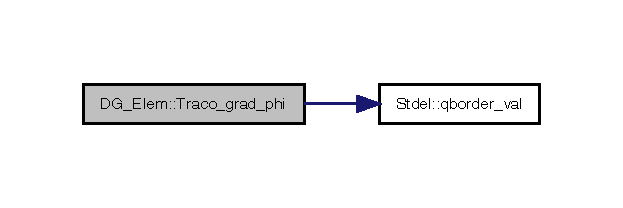
\includegraphics[width=299pt]{classDG__Elem_a8d090e18204cd99ed11ef8115a95c2e7_cgraph}
\end{center}
\end{figure}
Here is the caller graph for this function\+:
\nopagebreak
\begin{figure}[H]
\begin{center}
\leavevmode
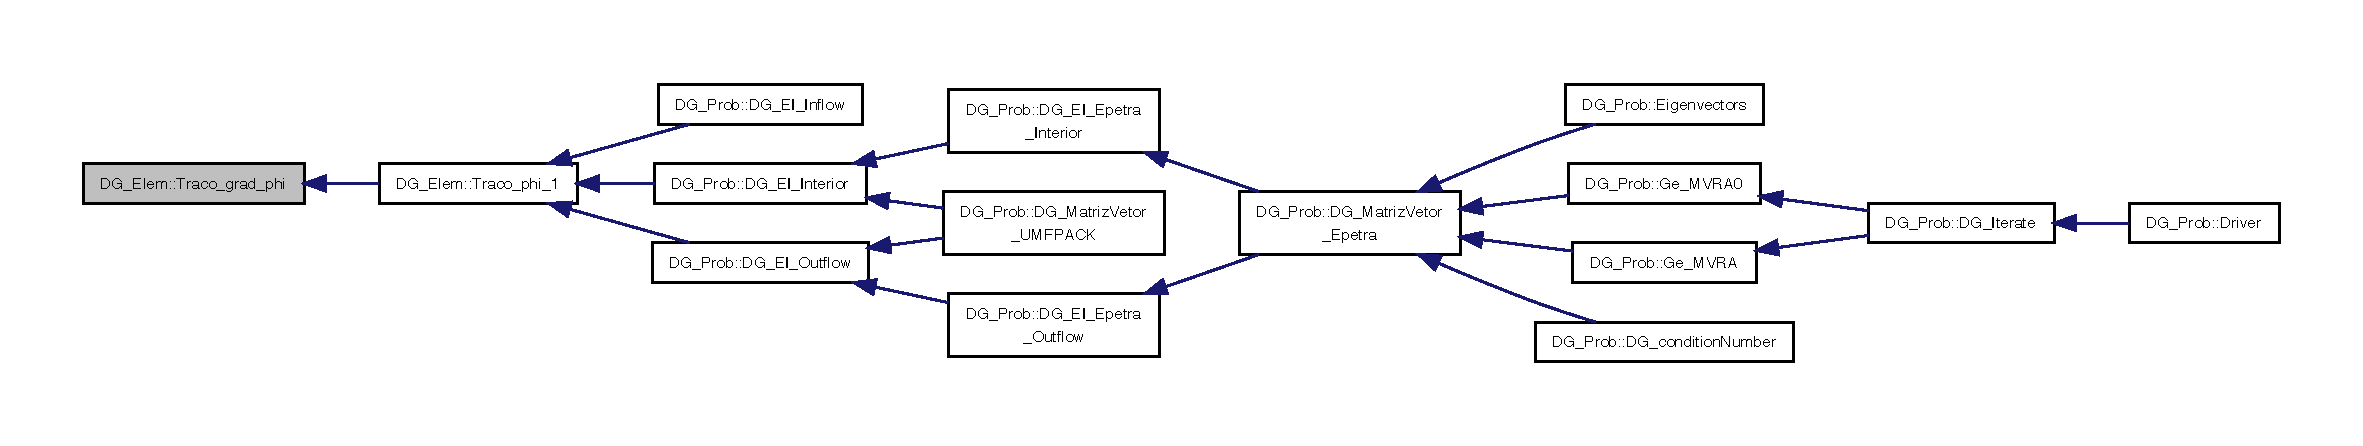
\includegraphics[width=350pt]{classDG__Elem_a8d090e18204cd99ed11ef8115a95c2e7_icgraph}
\end{center}
\end{figure}
\mbox{\Hypertarget{classDG__Elem_ad288d45acae59787b21a35b38fe47b10}\label{classDG__Elem_ad288d45acae59787b21a35b38fe47b10}} 
\index{D\+G\+\_\+\+Elem@{D\+G\+\_\+\+Elem}!Traco\+\_\+\+Kgrad\+\_\+pc@{Traco\+\_\+\+Kgrad\+\_\+pc}}
\index{Traco\+\_\+\+Kgrad\+\_\+pc@{Traco\+\_\+\+Kgrad\+\_\+pc}!D\+G\+\_\+\+Elem@{D\+G\+\_\+\+Elem}}
\subsubsection{\texorpdfstring{Traco\+\_\+\+Kgrad\+\_\+pc()}{Traco\_Kgrad\_pc()}}
{\footnotesize\ttfamily void D\+G\+\_\+\+Elem\+::\+Traco\+\_\+\+Kgrad\+\_\+pc (\begin{DoxyParamCaption}\item[{const int \&}]{h,  }\item[{double $\ast$$\ast$}]{saida }\end{DoxyParamCaption})}



Definition at line 432 of file D\+G\+\_\+\+Elem.\+cpp.



References Ph\+Elem$<$ 2 $>$\+::ndim, Ph\+Elem$<$ 2 $>$\+::ptr\+\_\+stdel, Stdel\+::qborder\+\_\+val(), qmax, and Tr\+Kgrad\+\_\+pc.



Referenced by D\+G\+\_\+\+Prob\+::\+D\+G\+\_\+\+E\+I\+\_\+flux(), D\+G\+\_\+\+Prob\+::\+D\+G\+\_\+\+E\+I\+\_\+\+I\+G(), for(), and show\+\_\+\+Volume().

Here is the call graph for this function\+:
\nopagebreak
\begin{figure}[H]
\begin{center}
\leavevmode
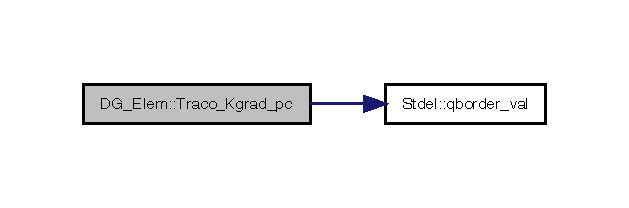
\includegraphics[width=302pt]{classDG__Elem_ad288d45acae59787b21a35b38fe47b10_cgraph}
\end{center}
\end{figure}
Here is the caller graph for this function\+:
\nopagebreak
\begin{figure}[H]
\begin{center}
\leavevmode
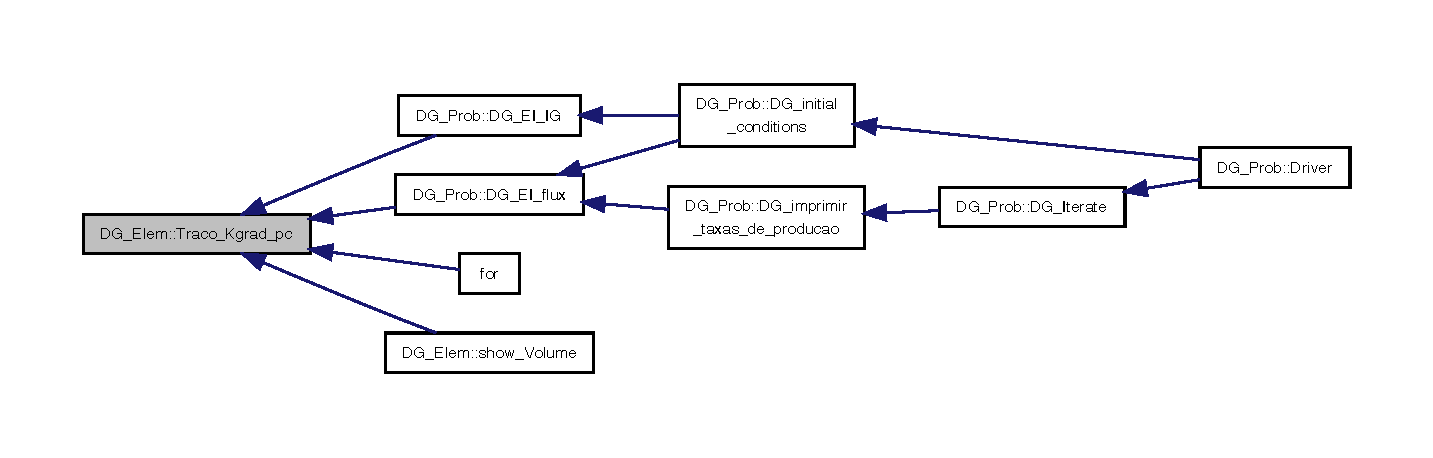
\includegraphics[width=350pt]{classDG__Elem_ad288d45acae59787b21a35b38fe47b10_icgraph}
\end{center}
\end{figure}
\mbox{\Hypertarget{classDG__Elem_a0109cc28854e31b5df555513e9fccfed}\label{classDG__Elem_a0109cc28854e31b5df555513e9fccfed}} 
\index{D\+G\+\_\+\+Elem@{D\+G\+\_\+\+Elem}!Traco\+\_\+\+Kgrad\+\_\+phi\+\_\+n@{Traco\+\_\+\+Kgrad\+\_\+phi\+\_\+n}}
\index{Traco\+\_\+\+Kgrad\+\_\+phi\+\_\+n@{Traco\+\_\+\+Kgrad\+\_\+phi\+\_\+n}!D\+G\+\_\+\+Elem@{D\+G\+\_\+\+Elem}}
\subsubsection{\texorpdfstring{Traco\+\_\+\+Kgrad\+\_\+phi\+\_\+n()}{Traco\_Kgrad\_phi\_n()}}
{\footnotesize\ttfamily void D\+G\+\_\+\+Elem\+::\+Traco\+\_\+\+Kgrad\+\_\+phi\+\_\+n (\begin{DoxyParamCaption}\item[{const int \&}]{lado,  }\item[{const int \&}]{ivar,  }\item[{const int \&}]{ind,  }\item[{double $\ast$}]{saida }\end{DoxyParamCaption})}



Definition at line 483 of file D\+G\+\_\+\+Elem.\+cpp.



References Ph\+Elem$<$ 2 $>$\+::ptr\+\_\+stdel, Stdel\+::qborder\+\_\+val(), qmax, and Tr\+Kgrad\+Phi\+\_\+n.



Referenced by D\+G\+\_\+\+Prob\+::\+D\+G\+\_\+\+E\+I\+\_\+\+I\+G(), for(), and Traco\+\_\+phi\+\_\+1().

Here is the call graph for this function\+:
\nopagebreak
\begin{figure}[H]
\begin{center}
\leavevmode
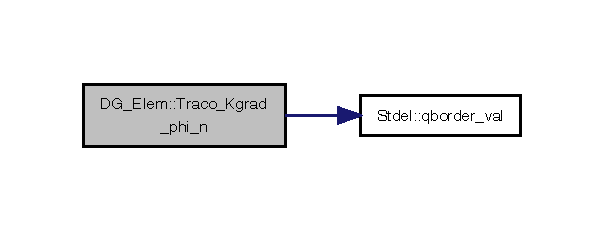
\includegraphics[width=290pt]{classDG__Elem_a0109cc28854e31b5df555513e9fccfed_cgraph}
\end{center}
\end{figure}
Here is the caller graph for this function\+:
\nopagebreak
\begin{figure}[H]
\begin{center}
\leavevmode
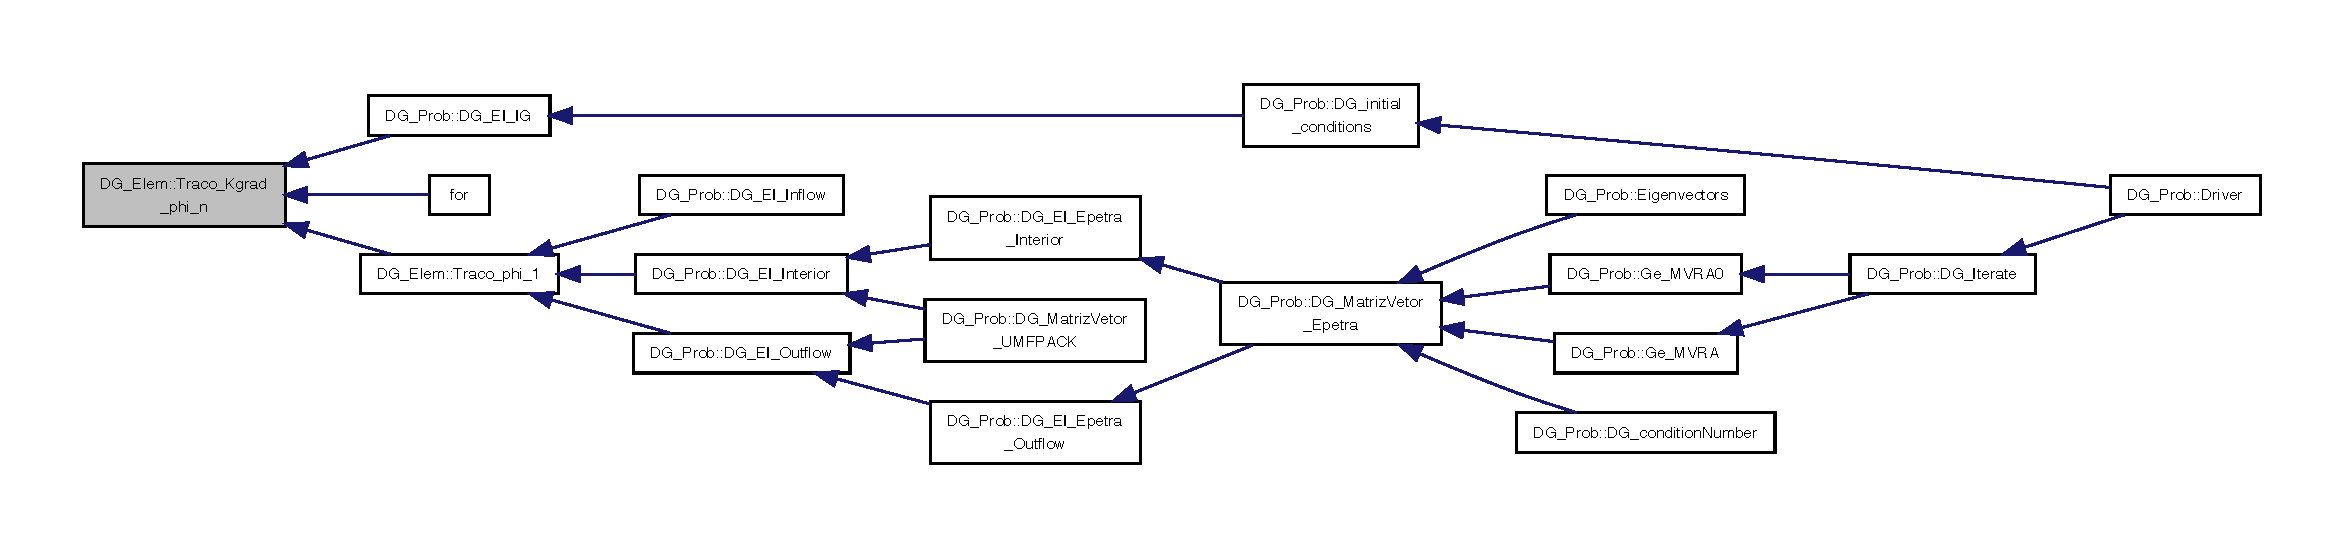
\includegraphics[width=350pt]{classDG__Elem_a0109cc28854e31b5df555513e9fccfed_icgraph}
\end{center}
\end{figure}
\mbox{\Hypertarget{classDG__Elem_ae98efe920078bc5fd18eceee997d44a2}\label{classDG__Elem_ae98efe920078bc5fd18eceee997d44a2}} 
\index{D\+G\+\_\+\+Elem@{D\+G\+\_\+\+Elem}!Traco\+\_\+\+Kgrad\+\_\+pw@{Traco\+\_\+\+Kgrad\+\_\+pw}}
\index{Traco\+\_\+\+Kgrad\+\_\+pw@{Traco\+\_\+\+Kgrad\+\_\+pw}!D\+G\+\_\+\+Elem@{D\+G\+\_\+\+Elem}}
\subsubsection{\texorpdfstring{Traco\+\_\+\+Kgrad\+\_\+pw()}{Traco\_Kgrad\_pw()}}
{\footnotesize\ttfamily void D\+G\+\_\+\+Elem\+::\+Traco\+\_\+\+Kgrad\+\_\+pw (\begin{DoxyParamCaption}\item[{const int \&}]{h,  }\item[{double $\ast$$\ast$}]{saida }\end{DoxyParamCaption})}



Definition at line 422 of file D\+G\+\_\+\+Elem.\+cpp.



References Ph\+Elem$<$ 2 $>$\+::ndim, Ph\+Elem$<$ 2 $>$\+::ptr\+\_\+stdel, Stdel\+::qborder\+\_\+val(), qmax, and Tr\+Kgrad\+\_\+pw.



Referenced by D\+G\+\_\+\+Prob\+::\+D\+G\+\_\+\+E\+I\+\_\+flux(), D\+G\+\_\+\+Prob\+::\+D\+G\+\_\+\+E\+I\+\_\+\+I\+G(), for(), and show\+\_\+\+Volume().

Here is the call graph for this function\+:
\nopagebreak
\begin{figure}[H]
\begin{center}
\leavevmode
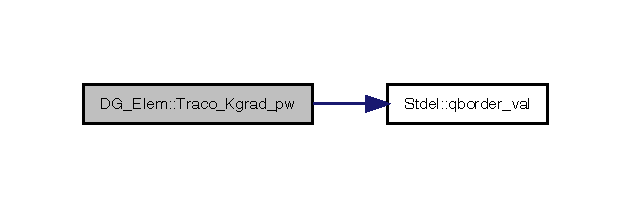
\includegraphics[width=303pt]{classDG__Elem_ae98efe920078bc5fd18eceee997d44a2_cgraph}
\end{center}
\end{figure}
Here is the caller graph for this function\+:
\nopagebreak
\begin{figure}[H]
\begin{center}
\leavevmode
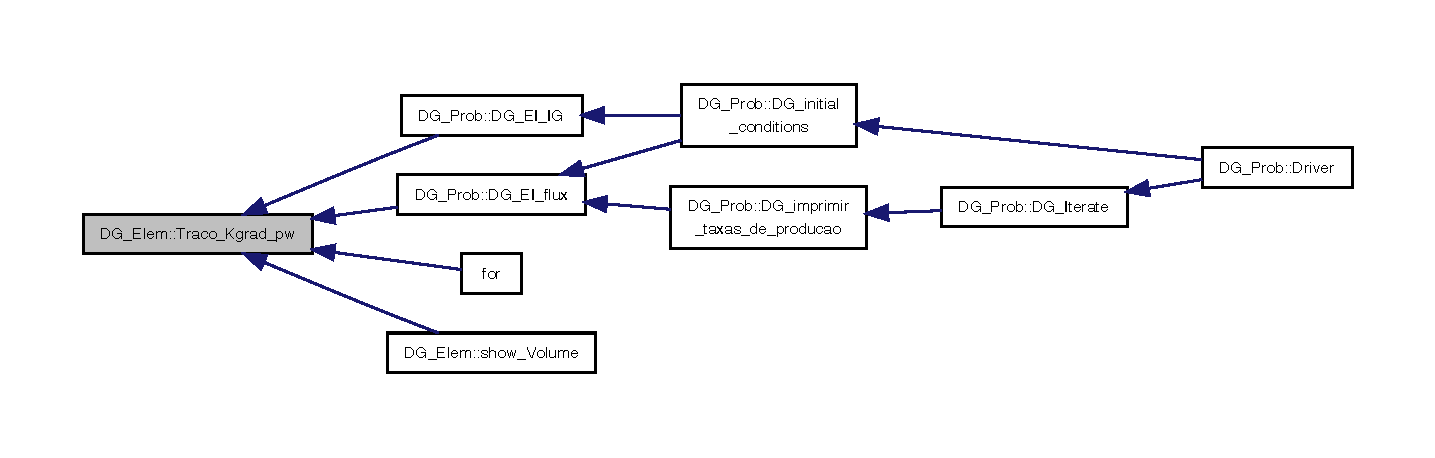
\includegraphics[width=350pt]{classDG__Elem_ae98efe920078bc5fd18eceee997d44a2_icgraph}
\end{center}
\end{figure}
\mbox{\Hypertarget{classDG__Elem_ae64a1118040aad9dd3c18ac68b2d5d4f}\label{classDG__Elem_ae64a1118040aad9dd3c18ac68b2d5d4f}} 
\index{D\+G\+\_\+\+Elem@{D\+G\+\_\+\+Elem}!Traco\+\_\+\+Kgrad\+\_\+sn@{Traco\+\_\+\+Kgrad\+\_\+sn}}
\index{Traco\+\_\+\+Kgrad\+\_\+sn@{Traco\+\_\+\+Kgrad\+\_\+sn}!D\+G\+\_\+\+Elem@{D\+G\+\_\+\+Elem}}
\subsubsection{\texorpdfstring{Traco\+\_\+\+Kgrad\+\_\+sn()}{Traco\_Kgrad\_sn()}}
{\footnotesize\ttfamily void D\+G\+\_\+\+Elem\+::\+Traco\+\_\+\+Kgrad\+\_\+sn (\begin{DoxyParamCaption}\item[{const int \&}]{h,  }\item[{double $\ast$$\ast$}]{saida }\end{DoxyParamCaption})}



Definition at line 442 of file D\+G\+\_\+\+Elem.\+cpp.



References Ph\+Elem$<$ 2 $>$\+::ndim, Ph\+Elem$<$ 2 $>$\+::ptr\+\_\+stdel, Stdel\+::qborder\+\_\+val(), qmax, and Tr\+Kgrad\+\_\+sn.



Referenced by D\+G\+\_\+\+Prob\+::\+D\+G\+\_\+\+E\+I\+\_\+\+I\+G(), for(), and show\+\_\+\+Volume().

Here is the call graph for this function\+:
\nopagebreak
\begin{figure}[H]
\begin{center}
\leavevmode
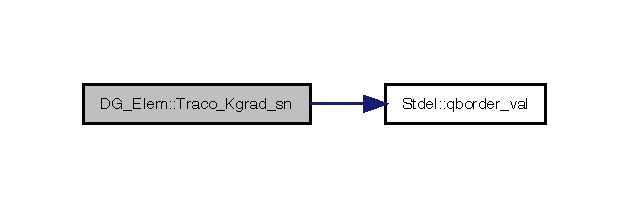
\includegraphics[width=302pt]{classDG__Elem_ae64a1118040aad9dd3c18ac68b2d5d4f_cgraph}
\end{center}
\end{figure}
Here is the caller graph for this function\+:
\nopagebreak
\begin{figure}[H]
\begin{center}
\leavevmode
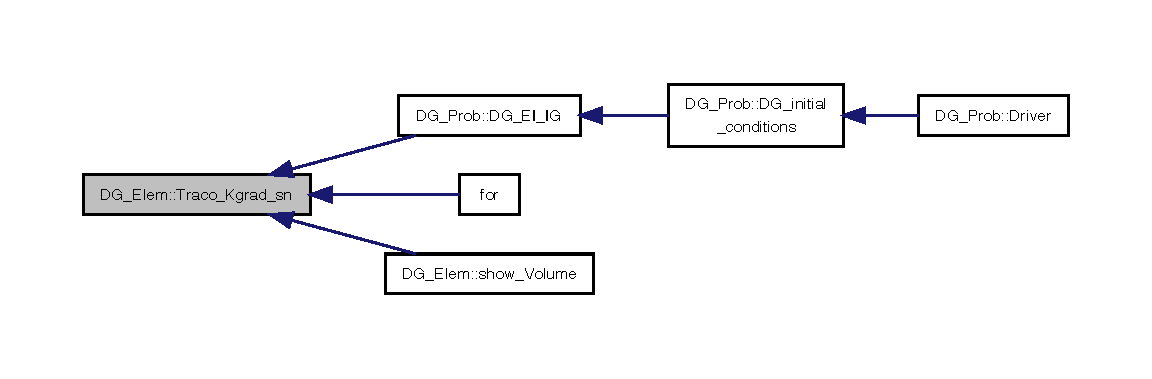
\includegraphics[width=350pt]{classDG__Elem_ae64a1118040aad9dd3c18ac68b2d5d4f_icgraph}
\end{center}
\end{figure}
\mbox{\Hypertarget{classDG__Elem_aa97824992d60c2a7b5506e5d660dc7a1}\label{classDG__Elem_aa97824992d60c2a7b5506e5d660dc7a1}} 
\index{D\+G\+\_\+\+Elem@{D\+G\+\_\+\+Elem}!Traco\+\_\+phi@{Traco\+\_\+phi}}
\index{Traco\+\_\+phi@{Traco\+\_\+phi}!D\+G\+\_\+\+Elem@{D\+G\+\_\+\+Elem}}
\subsubsection{\texorpdfstring{Traco\+\_\+phi()}{Traco\_phi()}}
{\footnotesize\ttfamily void D\+G\+\_\+\+Elem\+::\+Traco\+\_\+phi (\begin{DoxyParamCaption}\item[{const int \&}]{lado,  }\item[{const int \&}]{ivar,  }\item[{const int \&}]{ind,  }\item[{double $\ast$}]{saida }\end{DoxyParamCaption})}



Definition at line 454 of file D\+G\+\_\+\+Elem.\+cpp.



References pos, Ph\+Elem$<$ 2 $>$\+::ptr\+\_\+stdel, Stdel\+::qborder\+\_\+val(), qmax, and Tr\+Phi.



Referenced by D\+G\+\_\+\+Prob\+::\+D\+G\+\_\+\+E\+I\+\_\+\+I\+G(), and show\+\_\+\+Volume().

Here is the call graph for this function\+:
\nopagebreak
\begin{figure}[H]
\begin{center}
\leavevmode
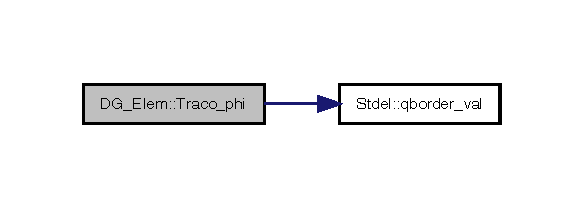
\includegraphics[width=280pt]{classDG__Elem_aa97824992d60c2a7b5506e5d660dc7a1_cgraph}
\end{center}
\end{figure}
Here is the caller graph for this function\+:
\nopagebreak
\begin{figure}[H]
\begin{center}
\leavevmode
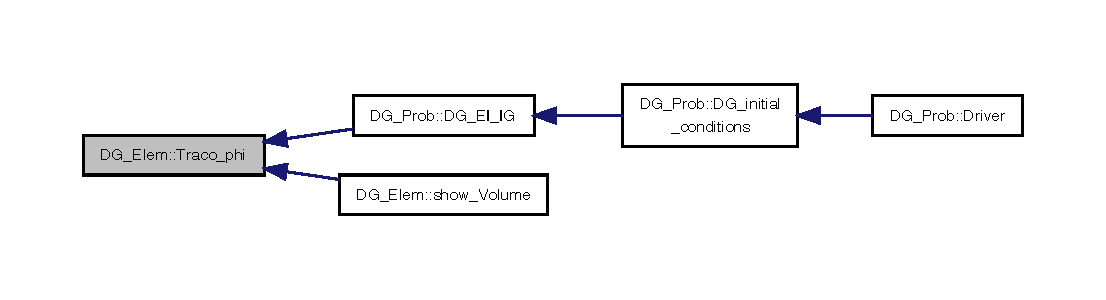
\includegraphics[width=350pt]{classDG__Elem_aa97824992d60c2a7b5506e5d660dc7a1_icgraph}
\end{center}
\end{figure}
\mbox{\Hypertarget{classDG__Elem_a99f9e69fc0d6eacd683712bc456af5f7}\label{classDG__Elem_a99f9e69fc0d6eacd683712bc456af5f7}} 
\index{D\+G\+\_\+\+Elem@{D\+G\+\_\+\+Elem}!Traco\+\_\+phi\+\_\+1@{Traco\+\_\+phi\+\_\+1}}
\index{Traco\+\_\+phi\+\_\+1@{Traco\+\_\+phi\+\_\+1}!D\+G\+\_\+\+Elem@{D\+G\+\_\+\+Elem}}
\subsubsection{\texorpdfstring{Traco\+\_\+phi\+\_\+1()}{Traco\_phi\_1()}}
{\footnotesize\ttfamily void D\+G\+\_\+\+Elem\+::\+Traco\+\_\+phi\+\_\+1 (\begin{DoxyParamCaption}\item[{const int \&}]{lado,  }\item[{const int \&}]{ivar,  }\item[{const int \&}]{pos,  }\item[{double $\ast$}]{saida }\end{DoxyParamCaption})\hspace{0.3cm}{\ttfamily [inline]}}



Definition at line 81 of file D\+G\+\_\+\+Elem.\+hpp.



References Ph\+Elem$<$ 2 $>$\+::ptr\+\_\+stdel, Stdel\+::qborder\+\_\+val(), qmax, Traco\+\_\+grad\+\_\+phi(), Traco\+\_\+\+Kgrad\+\_\+phi\+\_\+n(), and Tr\+Phi.



Referenced by D\+G\+\_\+\+Prob\+::\+D\+G\+\_\+\+E\+I\+\_\+\+Inflow(), D\+G\+\_\+\+Prob\+::\+D\+G\+\_\+\+E\+I\+\_\+\+Interior(), and D\+G\+\_\+\+Prob\+::\+D\+G\+\_\+\+E\+I\+\_\+\+Outflow().

Here is the call graph for this function\+:
\nopagebreak
\begin{figure}[H]
\begin{center}
\leavevmode
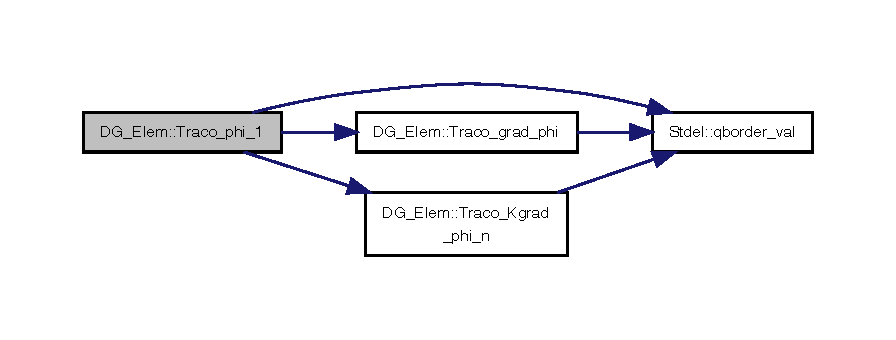
\includegraphics[width=350pt]{classDG__Elem_a99f9e69fc0d6eacd683712bc456af5f7_cgraph}
\end{center}
\end{figure}
Here is the caller graph for this function\+:
\nopagebreak
\begin{figure}[H]
\begin{center}
\leavevmode
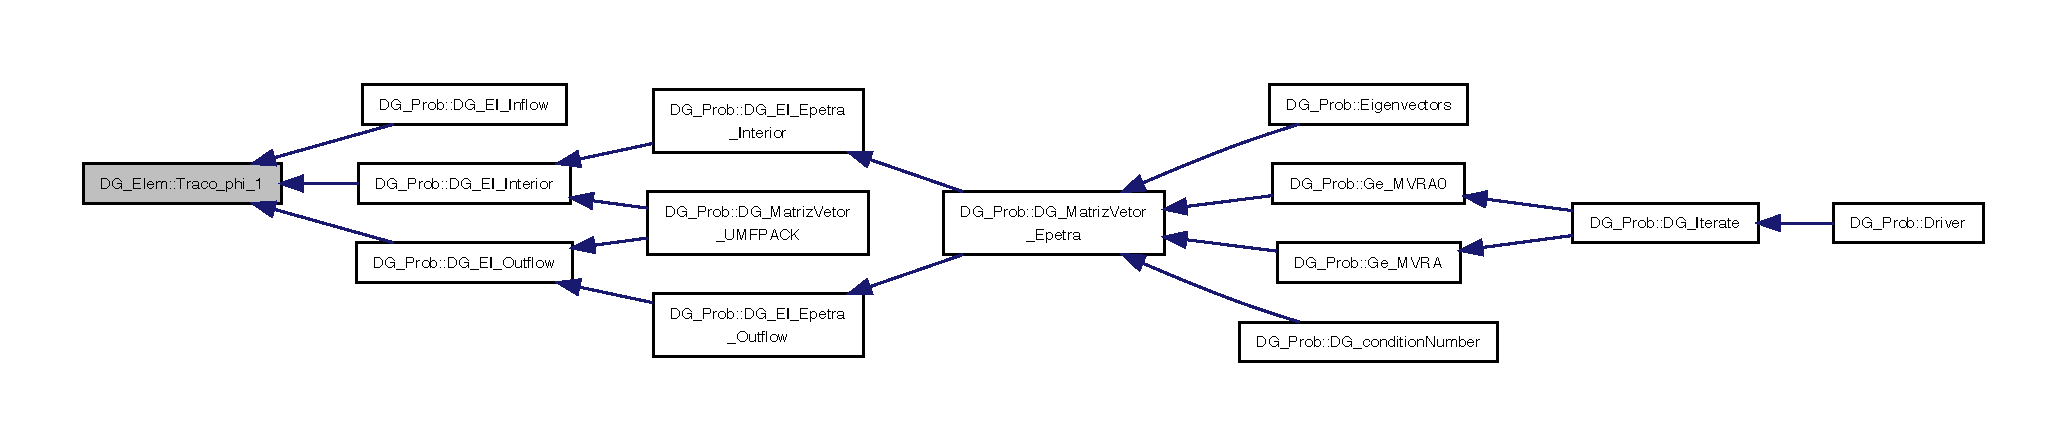
\includegraphics[width=350pt]{classDG__Elem_a99f9e69fc0d6eacd683712bc456af5f7_icgraph}
\end{center}
\end{figure}
\mbox{\Hypertarget{classDG__Elem_ab57a34a01c448785d8a887e51e7ab331}\label{classDG__Elem_ab57a34a01c448785d8a887e51e7ab331}} 
\index{D\+G\+\_\+\+Elem@{D\+G\+\_\+\+Elem}!Traco\+\_\+pw@{Traco\+\_\+pw}}
\index{Traco\+\_\+pw@{Traco\+\_\+pw}!D\+G\+\_\+\+Elem@{D\+G\+\_\+\+Elem}}
\subsubsection{\texorpdfstring{Traco\+\_\+pw()}{Traco\_pw()}}
{\footnotesize\ttfamily void D\+G\+\_\+\+Elem\+::\+Traco\+\_\+pw (\begin{DoxyParamCaption}\item[{const int \&}]{h,  }\item[{double $\ast$}]{saida }\end{DoxyParamCaption})}



Definition at line 415 of file D\+G\+\_\+\+Elem.\+cpp.



References Ph\+Elem$<$ 2 $>$\+::ptr\+\_\+stdel, Stdel\+::qborder\+\_\+val(), qmax, and Trpw.



Referenced by D\+G\+\_\+\+Prob\+::\+D\+G\+\_\+\+E\+I\+\_\+\+I\+G(), and show\+\_\+\+Volume().

Here is the call graph for this function\+:
\nopagebreak
\begin{figure}[H]
\begin{center}
\leavevmode
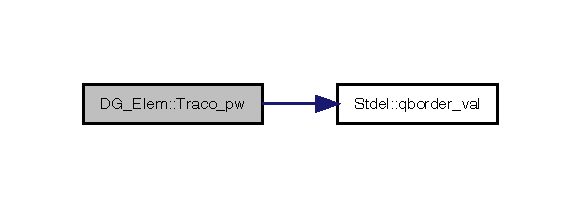
\includegraphics[width=279pt]{classDG__Elem_ab57a34a01c448785d8a887e51e7ab331_cgraph}
\end{center}
\end{figure}
Here is the caller graph for this function\+:
\nopagebreak
\begin{figure}[H]
\begin{center}
\leavevmode
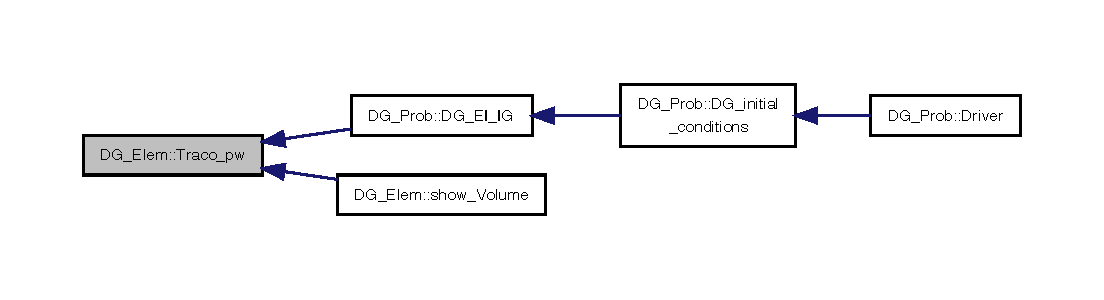
\includegraphics[width=350pt]{classDG__Elem_ab57a34a01c448785d8a887e51e7ab331_icgraph}
\end{center}
\end{figure}
\mbox{\Hypertarget{classDG__Elem_a4b5b26372a103e9f10c9d518419d4fd1}\label{classDG__Elem_a4b5b26372a103e9f10c9d518419d4fd1}} 
\index{D\+G\+\_\+\+Elem@{D\+G\+\_\+\+Elem}!Traco\+\_\+sn@{Traco\+\_\+sn}}
\index{Traco\+\_\+sn@{Traco\+\_\+sn}!D\+G\+\_\+\+Elem@{D\+G\+\_\+\+Elem}}
\subsubsection{\texorpdfstring{Traco\+\_\+sn()}{Traco\_sn()}}
{\footnotesize\ttfamily void D\+G\+\_\+\+Elem\+::\+Traco\+\_\+sn (\begin{DoxyParamCaption}\item[{const int \&}]{h,  }\item[{double $\ast$}]{saida }\end{DoxyParamCaption})}



Definition at line 408 of file D\+G\+\_\+\+Elem.\+cpp.



References Ph\+Elem$<$ 2 $>$\+::ptr\+\_\+stdel, Stdel\+::qborder\+\_\+val(), qmax, and Trsn.



Referenced by D\+G\+\_\+\+Prob\+::\+D\+G\+\_\+\+E\+I\+\_\+\+I\+G(), and show\+\_\+\+Volume().

Here is the call graph for this function\+:
\nopagebreak
\begin{figure}[H]
\begin{center}
\leavevmode
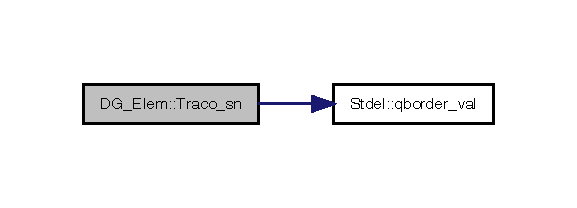
\includegraphics[width=277pt]{classDG__Elem_a4b5b26372a103e9f10c9d518419d4fd1_cgraph}
\end{center}
\end{figure}
Here is the caller graph for this function\+:
\nopagebreak
\begin{figure}[H]
\begin{center}
\leavevmode
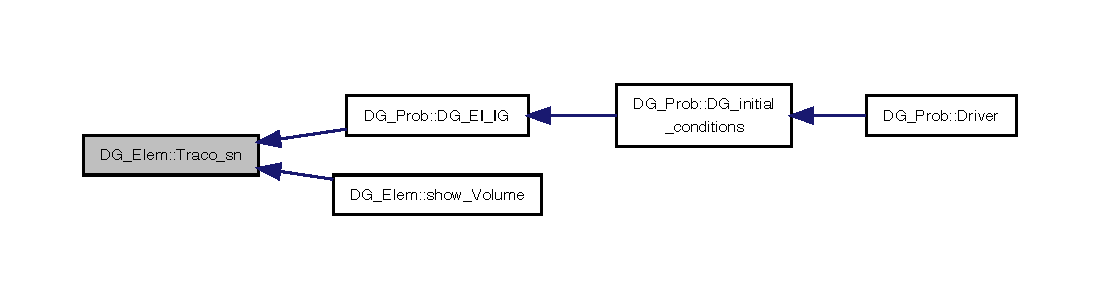
\includegraphics[width=350pt]{classDG__Elem_a4b5b26372a103e9f10c9d518419d4fd1_icgraph}
\end{center}
\end{figure}
\mbox{\Hypertarget{classPhElem_a09b6787e5e42496ece86754bbb2ae59c}\label{classPhElem_a09b6787e5e42496ece86754bbb2ae59c}} 
\index{D\+G\+\_\+\+Elem@{D\+G\+\_\+\+Elem}!transformacao\+\_\+direta@{transformacao\+\_\+direta}}
\index{transformacao\+\_\+direta@{transformacao\+\_\+direta}!D\+G\+\_\+\+Elem@{D\+G\+\_\+\+Elem}}
\subsubsection{\texorpdfstring{transformacao\+\_\+direta()}{transformacao\_direta()}}
{\footnotesize\ttfamily void \hyperlink{classPhElem}{Ph\+Elem}$<$ Num\+Variaveis $>$\+::transformacao\+\_\+direta (\begin{DoxyParamCaption}\item[{double}]{f\mbox{[}$\,$\mbox{]},  }\item[{const int \&}]{ivar }\end{DoxyParamCaption})\hspace{0.3cm}{\ttfamily [inherited]}}



Definition at line 980 of file Ph\+Elem.\+hpp.



References aux, B(), Ph\+Elem$<$ Num\+Variaveis $>$\+::\+JV, Stdel\+::mass(), Ph\+Elem$<$ Num\+Variaveis $>$\+::numn, Ph\+Elem$<$ Num\+Variaveis $>$\+::ptr\+\_\+stdel, Ph\+Elem$<$ Num\+Variaveis $>$\+::u0, and Stdel\+::vector\+\_\+of\+\_\+integral\+\_\+of\+\_\+f\+\_\+\+Phi\+\_\+dv().

\mbox{\Hypertarget{classPhElem_a4ea6c54e35eb46d331db770f992c4c4b}\label{classPhElem_a4ea6c54e35eb46d331db770f992c4c4b}} 
\index{D\+G\+\_\+\+Elem@{D\+G\+\_\+\+Elem}!type\+\_\+val@{type\+\_\+val}}
\index{type\+\_\+val@{type\+\_\+val}!D\+G\+\_\+\+Elem@{D\+G\+\_\+\+Elem}}
\subsubsection{\texorpdfstring{type\+\_\+val()}{type\_val()}}
{\footnotesize\ttfamily int \hyperlink{classPhElem}{Ph\+Elem}$<$ Num\+Variaveis $>$\+::type\+\_\+val (\begin{DoxyParamCaption}{ }\end{DoxyParamCaption})\hspace{0.3cm}{\ttfamily [inherited]}}



Definition at line 535 of file Ph\+Elem.\+hpp.



References Ph\+Elem$<$ Num\+Variaveis $>$\+::type.

\mbox{\Hypertarget{classPhElem_a38499c9f62a291a880d72db646171cb5}\label{classPhElem_a38499c9f62a291a880d72db646171cb5}} 
\index{D\+G\+\_\+\+Elem@{D\+G\+\_\+\+Elem}!Vector\+Elast2D@{Vector\+Elast2D}}
\index{Vector\+Elast2D@{Vector\+Elast2D}!D\+G\+\_\+\+Elem@{D\+G\+\_\+\+Elem}}
\subsubsection{\texorpdfstring{Vector\+Elast2\+D()}{VectorElast2D()}\hspace{0.1cm}{\footnotesize\ttfamily [1/2]}}
{\footnotesize\ttfamily void \hyperlink{classPhElem}{Ph\+Elem}$<$ Num\+Variaveis $>$\+::Vector\+Elast2D (\begin{DoxyParamCaption}\item[{const int \&}]{i,  }\item[{double}]{sum\mbox{[}$\,$\mbox{]} }\end{DoxyParamCaption})\hspace{0.3cm}{\ttfamily [inherited]}}

\mbox{\Hypertarget{classPhElem_a4b130cb327652894d81b2c4e26b96f41}\label{classPhElem_a4b130cb327652894d81b2c4e26b96f41}} 
\index{D\+G\+\_\+\+Elem@{D\+G\+\_\+\+Elem}!Vector\+Elast2D@{Vector\+Elast2D}}
\index{Vector\+Elast2D@{Vector\+Elast2D}!D\+G\+\_\+\+Elem@{D\+G\+\_\+\+Elem}}
\subsubsection{\texorpdfstring{Vector\+Elast2\+D()}{VectorElast2D()}\hspace{0.1cm}{\footnotesize\ttfamily [2/2]}}
{\footnotesize\ttfamily void \hyperlink{classPhElem}{Ph\+Elem}$<$ Num\+Variaveis $>$\+::Vector\+Elast2D (\begin{DoxyParamCaption}\item[{double}]{vector\mbox{[}$\,$\mbox{]} }\end{DoxyParamCaption})\hspace{0.3cm}{\ttfamily [inherited]}}



Definition at line 161 of file Elastostatica.\+cpp.



References Ph\+Elem$<$ Num\+Variaveis $>$\+::b0, and Ph\+Elem$<$ Num\+Variaveis $>$\+::sgn.

\mbox{\Hypertarget{classPhElem_a993d5f1b66f6d99ffb95adc9ff882e80}\label{classPhElem_a993d5f1b66f6d99ffb95adc9ff882e80}} 
\index{D\+G\+\_\+\+Elem@{D\+G\+\_\+\+Elem}!vetor\+\_\+superficie@{vetor\+\_\+superficie}}
\index{vetor\+\_\+superficie@{vetor\+\_\+superficie}!D\+G\+\_\+\+Elem@{D\+G\+\_\+\+Elem}}
\subsubsection{\texorpdfstring{vetor\+\_\+superficie()}{vetor\_superficie()}}
{\footnotesize\ttfamily void \hyperlink{classPhElem}{Ph\+Elem}$<$ Num\+Variaveis $>$\+::vetor\+\_\+superficie (\begin{DoxyParamCaption}\item[{const int \&}]{num\+\_\+local,  }\item[{double \&}]{area,  }\item[{double}]{normal\mbox{[}3\mbox{]} }\end{DoxyParamCaption})\hspace{0.3cm}{\ttfamily [inherited]}}



Definition at line 1487 of file Ph\+Elem.\+hpp.



References Ph\+Elem$<$ Num\+Variaveis $>$\+::ptr\+\_\+stdel, Ph\+Elem$<$ Num\+Variaveis $>$\+::ptvert, Stdel\+::superficie\+\_\+externa(), and Ph\+Elem$<$ Num\+Variaveis $>$\+::\+Vert\+\_\+map.

\mbox{\Hypertarget{classDG__Elem_a166b7ad0ea852f703f65661c14b5c713}\label{classDG__Elem_a166b7ad0ea852f703f65661c14b5c713}} 
\index{D\+G\+\_\+\+Elem@{D\+G\+\_\+\+Elem}!Volume\+Integrals@{Volume\+Integrals}}
\index{Volume\+Integrals@{Volume\+Integrals}!D\+G\+\_\+\+Elem@{D\+G\+\_\+\+Elem}}
\subsubsection{\texorpdfstring{Volume\+Integrals()}{VolumeIntegrals()}}
{\footnotesize\ttfamily void D\+G\+\_\+\+Elem\+::\+Volume\+Integrals (\begin{DoxyParamCaption}\item[{const double}]{Dt,  }\item[{\hyperlink{classFluids}{Fluids}}]{fls,  }\item[{Teuchos\+::\+R\+CP$<$ Epetra\+\_\+\+F\+E\+Crs\+Matrix $>$}]{A,  }\item[{Teuchos\+::\+R\+CP$<$ Epetra\+\_\+\+F\+E\+Vector $>$}]{R\+HS,  }\item[{double $\ast$}]{gbtrsn = {\ttfamily NULL},  }\item[{double $\ast$}]{gbtrpw = {\ttfamily NULL} }\end{DoxyParamCaption})}



Definition at line 1124 of file D\+G\+\_\+\+Elem.\+cpp.



References aaux, aux, B(), d2\+\_\+pc, Fluids\+::d2pc(), d\+\_\+lambdan, d\+\_\+lambdat, d\+\_\+lambdaw, d\+\_\+pc, Fluids\+::dkrn(), Fluids\+::dkrw(), Fluids\+::dpc(), Stdel\+::eval\+\_\+\+Phi(), Stdel\+::eval\+G\+Q(), Ph\+Elem$<$ 2 $>$\+::gbnmap, Ph\+Elem$<$ 2 $>$\+::gbtrbmap, Stdel\+::\+Gradiente(), Grad\+Phi, indice(), integral(), Ph\+Elem$<$ 2 $>$\+::\+JV, Fluids\+::\+Krn(), Fluids\+::\+Krw(), lambdan, lambdat, lambdaw, m, mun, muw, n0, Ph\+Elem$<$ 2 $>$\+::ndim, Stdel\+::\+N\+G\+Q\+P\+\_\+val(), npos(), Ph\+Elem$<$ 2 $>$\+::numborders, Ph\+Elem$<$ 2 $>$\+::numn, pc, perm, phi\+\_\+l, phi\+\_\+r, porosidade, pres, Fluids\+::pressao\+\_\+capilar(), Ph\+Elem$<$ 2 $>$\+::ptr\+\_\+stdel, Ph\+Elem$<$ 2 $>$\+::ptvert, pw, Stdel\+::qborder\+\_\+val(), qmax, qn, qw, sat, Fluids\+::show\+\_\+mun(), Fluids\+::show\+\_\+muw(), Ph\+Elem$<$ 2 $>$\+::sinal, sn, sna, Stdel\+::trace(), Tr\+Kgrad\+\_\+pc, Tr\+Kgrad\+\_\+pw, Tr\+Kgrad\+\_\+sn, Trpw, Trsn, Ph\+Elem$<$ 2 $>$\+::u0, and Ph\+Elem$<$ 2 $>$\+::\+Vert\+\_\+map.



Referenced by D\+G\+\_\+\+Prob\+::\+D\+G\+\_\+\+Matriz\+Vetor\+\_\+\+Epetra(), and show\+\_\+\+Volume().

Here is the call graph for this function\+:
\nopagebreak
\begin{figure}[H]
\begin{center}
\leavevmode
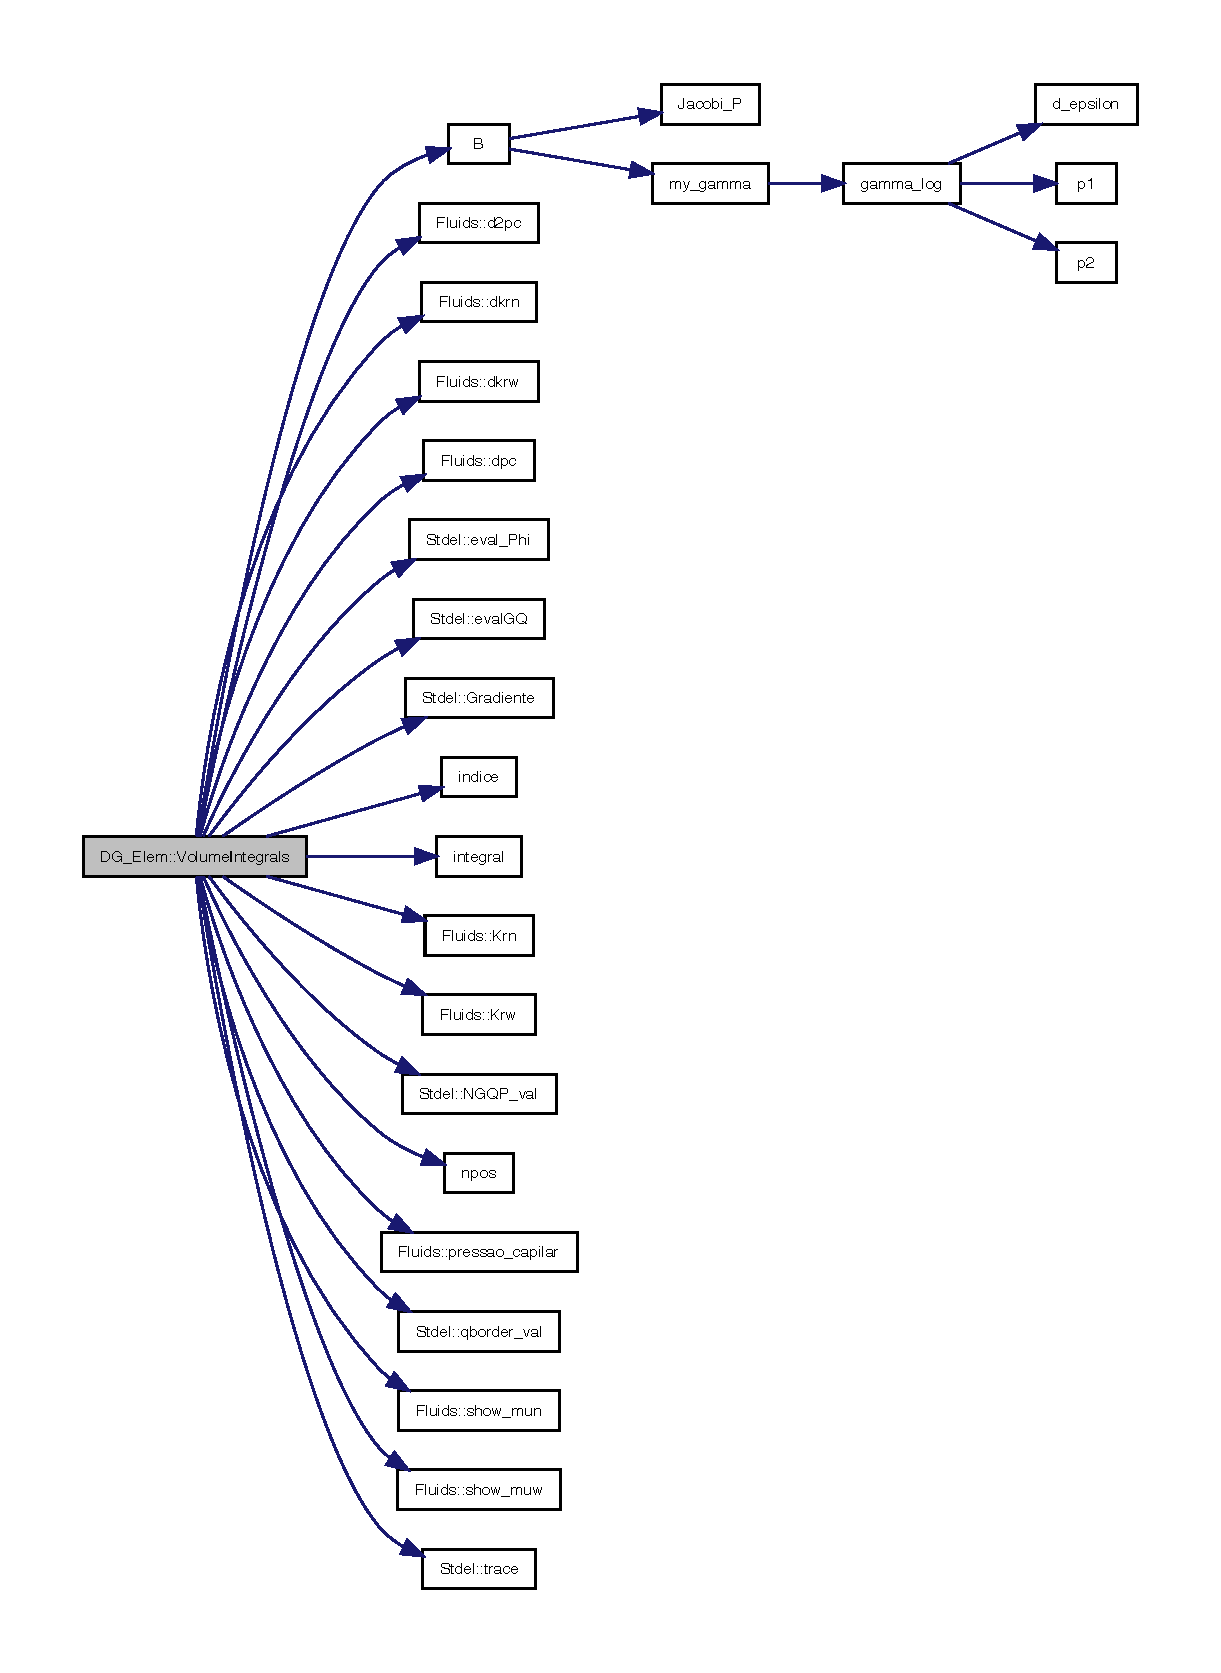
\includegraphics[width=350pt]{classDG__Elem_a166b7ad0ea852f703f65661c14b5c713_cgraph}
\end{center}
\end{figure}
Here is the caller graph for this function\+:
\nopagebreak
\begin{figure}[H]
\begin{center}
\leavevmode
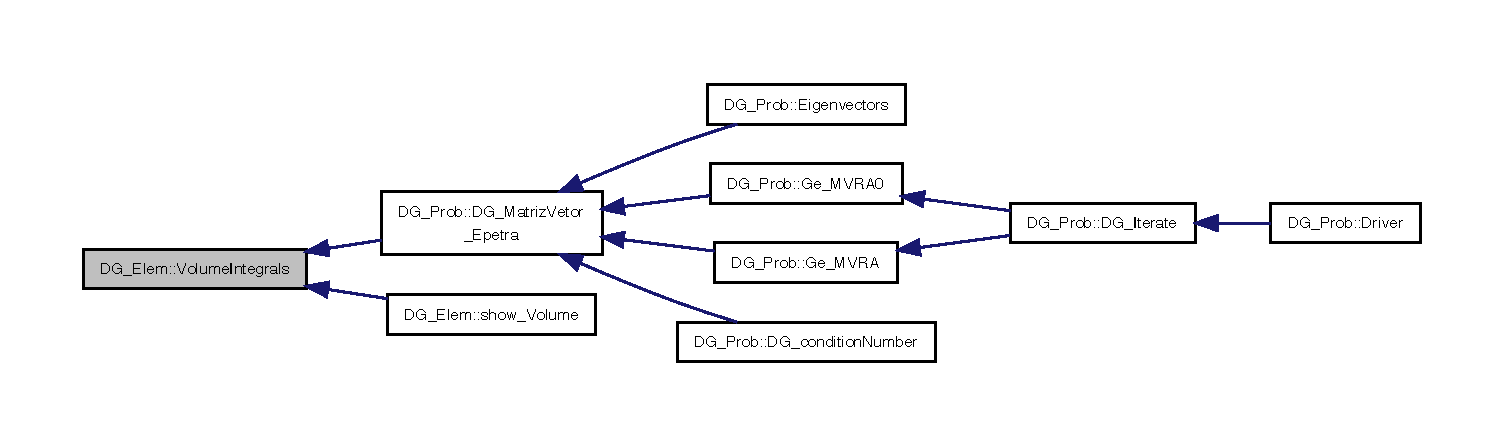
\includegraphics[width=350pt]{classDG__Elem_a166b7ad0ea852f703f65661c14b5c713_icgraph}
\end{center}
\end{figure}
\mbox{\Hypertarget{classDG__Elem_a3fc71dbfe141c0d42dc8ceff8f0ef8ce}\label{classDG__Elem_a3fc71dbfe141c0d42dc8ceff8f0ef8ce}} 
\index{D\+G\+\_\+\+Elem@{D\+G\+\_\+\+Elem}!Volume\+Integrals\+\_\+\+IG@{Volume\+Integrals\+\_\+\+IG}}
\index{Volume\+Integrals\+\_\+\+IG@{Volume\+Integrals\+\_\+\+IG}!D\+G\+\_\+\+Elem@{D\+G\+\_\+\+Elem}}
\subsubsection{\texorpdfstring{Volume\+Integrals\+\_\+\+I\+G()}{VolumeIntegrals\_IG()}}
{\footnotesize\ttfamily void D\+G\+\_\+\+Elem\+::\+Volume\+Integrals\+\_\+\+IG (\begin{DoxyParamCaption}\item[{\hyperlink{classFluids}{Fluids}}]{fls,  }\item[{int \&}]{count,  }\item[{int $\ast$}]{Ti,  }\item[{int $\ast$}]{Tj,  }\item[{double $\ast$}]{Tx,  }\item[{double $\ast$}]{B }\end{DoxyParamCaption})}



Definition at line 492 of file D\+G\+\_\+\+Elem.\+cpp.



References aux, d2\+\_\+pc, Fluids\+::d2pc(), d\+\_\+lambdan, d\+\_\+lambdat, d\+\_\+lambdaw, d\+\_\+pc, Fluids\+::dkrn(), Fluids\+::dkrw(), Fluids\+::dpc(), Stdel\+::eval\+G\+Q(), Ph\+Elem$<$ 2 $>$\+::gbnmap, Stdel\+::\+Gradiente(), Grad\+Phi, integral(), Ph\+Elem$<$ 2 $>$\+::\+JV, Fluids\+::\+Krn(), Fluids\+::\+Krw(), lambdan, lambdat, lambdaw, m, mun, muw, Ph\+Elem$<$ 2 $>$\+::ndim, Stdel\+::\+N\+G\+Q\+P\+\_\+val(), Ph\+Elem$<$ 2 $>$\+::numborders, Ph\+Elem$<$ 2 $>$\+::numn, pc, perm, pres, Fluids\+::pressao\+\_\+capilar(), prodev(), prodvv(), Ph\+Elem$<$ 2 $>$\+::ptr\+\_\+stdel, Ph\+Elem$<$ 2 $>$\+::ptvert, pw, Stdel\+::qborder\+\_\+val(), qmax, sat, Fluids\+::show\+\_\+mun(), Fluids\+::show\+\_\+muw(), Ph\+Elem$<$ 2 $>$\+::sinal, sn, somavv(), Stdel\+::trace(), Tr\+Kgrad\+\_\+pc, Tr\+Kgrad\+\_\+pw, Tr\+Kgrad\+\_\+sn, Trpw, Trsn, Ph\+Elem$<$ 2 $>$\+::u0, and Ph\+Elem$<$ 2 $>$\+::\+Vert\+\_\+map.



Referenced by D\+G\+\_\+\+Prob\+::\+D\+G\+\_\+initial\+\_\+conditions(), and show\+\_\+\+Volume().

Here is the call graph for this function\+:
\nopagebreak
\begin{figure}[H]
\begin{center}
\leavevmode
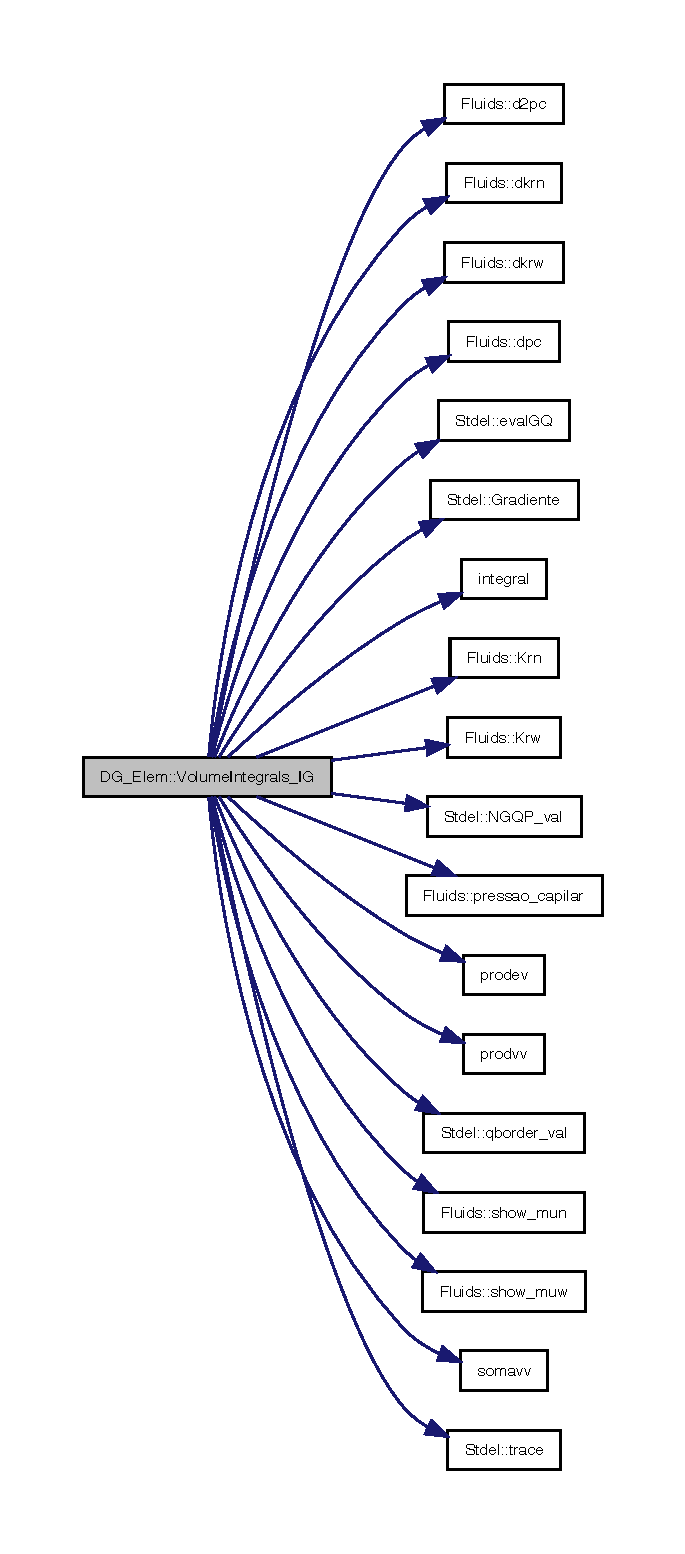
\includegraphics[height=550pt]{classDG__Elem_a3fc71dbfe141c0d42dc8ceff8f0ef8ce_cgraph}
\end{center}
\end{figure}
Here is the caller graph for this function\+:
\nopagebreak
\begin{figure}[H]
\begin{center}
\leavevmode
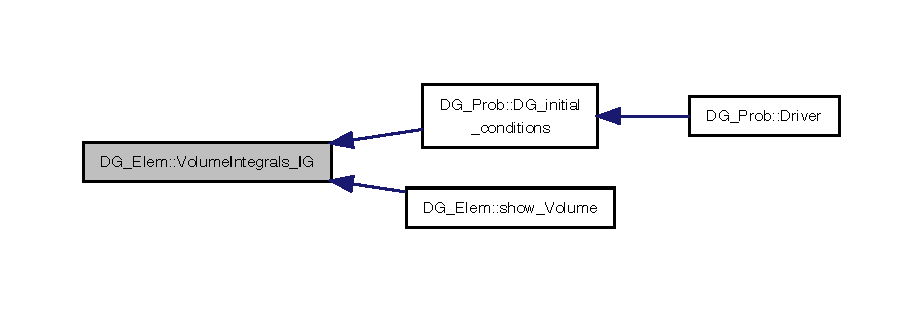
\includegraphics[width=350pt]{classDG__Elem_a3fc71dbfe141c0d42dc8ceff8f0ef8ce_icgraph}
\end{center}
\end{figure}
\mbox{\Hypertarget{classDG__Elem_ab3de164caf40da7cc0b123928ad83cc9}\label{classDG__Elem_ab3de164caf40da7cc0b123928ad83cc9}} 
\index{D\+G\+\_\+\+Elem@{D\+G\+\_\+\+Elem}!Volume\+Integrals\+\_\+\+U\+M\+F\+P\+A\+CK@{Volume\+Integrals\+\_\+\+U\+M\+F\+P\+A\+CK}}
\index{Volume\+Integrals\+\_\+\+U\+M\+F\+P\+A\+CK@{Volume\+Integrals\+\_\+\+U\+M\+F\+P\+A\+CK}!D\+G\+\_\+\+Elem@{D\+G\+\_\+\+Elem}}
\subsubsection{\texorpdfstring{Volume\+Integrals\+\_\+\+U\+M\+F\+P\+A\+C\+K()}{VolumeIntegrals\_UMFPACK()}}
{\footnotesize\ttfamily void D\+G\+\_\+\+Elem\+::\+Volume\+Integrals\+\_\+\+U\+M\+F\+P\+A\+CK (\begin{DoxyParamCaption}\item[{const double}]{Dt,  }\item[{\hyperlink{classFluids}{Fluids}}]{fls,  }\item[{int \&}]{count,  }\item[{int $\ast$}]{Ti,  }\item[{int $\ast$}]{Tj,  }\item[{double $\ast$}]{Tx,  }\item[{double $\ast$}]{B,  }\item[{double $\ast$}]{gbtrsn = {\ttfamily NULL},  }\item[{double $\ast$}]{gbtrpw = {\ttfamily NULL} }\end{DoxyParamCaption})}



Definition at line 635 of file D\+G\+\_\+\+Elem.\+cpp.



References aaux, aux, d2\+\_\+pc, Fluids\+::d2pc(), d\+\_\+lambdan, d\+\_\+lambdat, d\+\_\+lambdaw, d\+\_\+pc, Fluids\+::dkrn(), Fluids\+::dkrw(), Fluids\+::dpc(), Stdel\+::eval\+\_\+\+Phi(), Stdel\+::eval\+G\+Q(), Ph\+Elem$<$ 2 $>$\+::gbnmap, Ph\+Elem$<$ 2 $>$\+::gbtrbmap, Stdel\+::\+Gradiente(), Grad\+Phi, indice(), integral(), Ph\+Elem$<$ 2 $>$\+::\+JV, Fluids\+::\+Krn(), Fluids\+::\+Krw(), lambdan, lambdat, lambdaw, m, mun, muw, n0, Ph\+Elem$<$ 2 $>$\+::ndim, Stdel\+::\+N\+G\+Q\+P\+\_\+val(), npos(), Ph\+Elem$<$ 2 $>$\+::numborders, Ph\+Elem$<$ 2 $>$\+::numn, pc, perm, phi\+\_\+l, phi\+\_\+r, porosidade, pres, Fluids\+::pressao\+\_\+capilar(), Ph\+Elem$<$ 2 $>$\+::ptr\+\_\+stdel, Ph\+Elem$<$ 2 $>$\+::ptvert, pw, Stdel\+::qborder\+\_\+val(), qmax, qn, qw, sat, Fluids\+::show\+\_\+mun(), Fluids\+::show\+\_\+muw(), Ph\+Elem$<$ 2 $>$\+::sinal, sn, sna, Stdel\+::trace(), Tr\+Kgrad\+\_\+pc, Tr\+Kgrad\+\_\+pw, Tr\+Kgrad\+\_\+sn, Trpw, Trsn, Ph\+Elem$<$ 2 $>$\+::u0, and Ph\+Elem$<$ 2 $>$\+::\+Vert\+\_\+map.



Referenced by D\+G\+\_\+\+Prob\+::\+D\+G\+\_\+\+Matriz\+Vetor\+\_\+\+U\+M\+F\+P\+A\+C\+K(), and show\+\_\+\+Volume().

Here is the call graph for this function\+:
\nopagebreak
\begin{figure}[H]
\begin{center}
\leavevmode
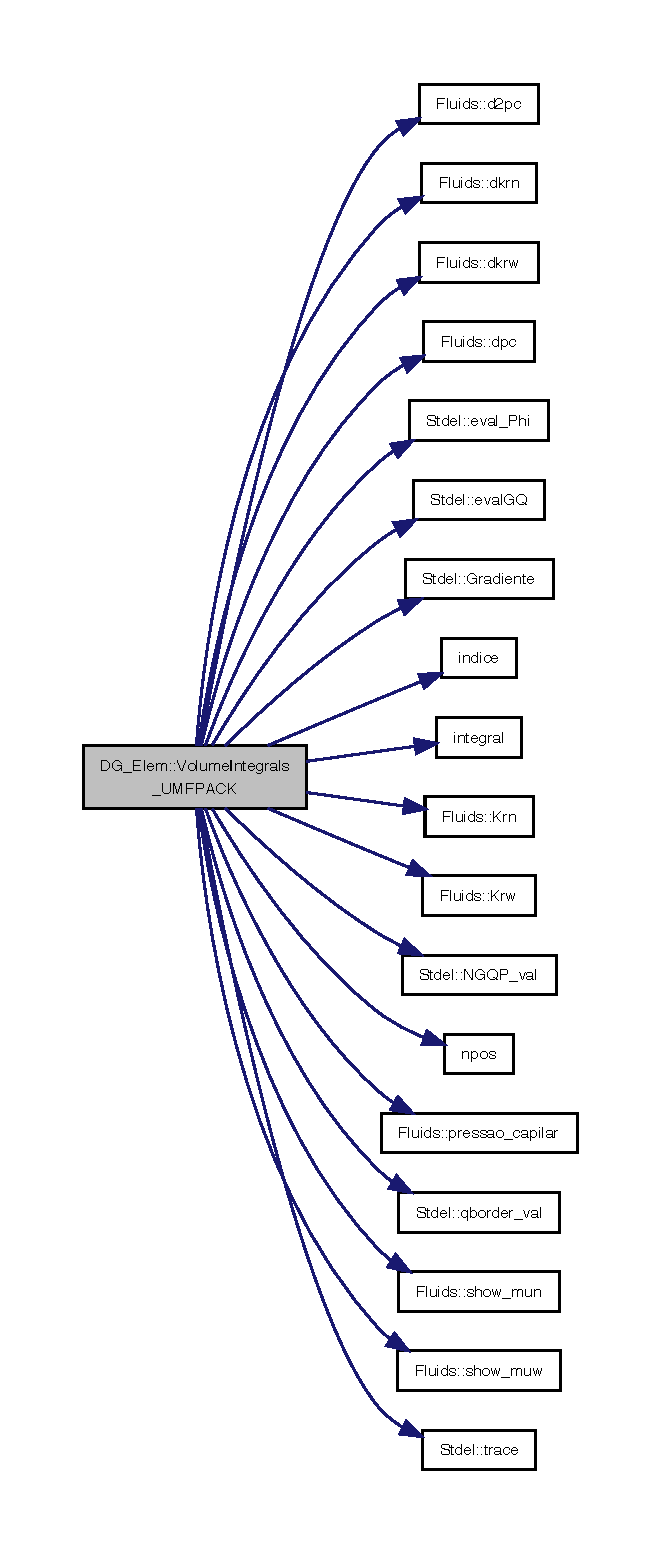
\includegraphics[height=550pt]{classDG__Elem_ab3de164caf40da7cc0b123928ad83cc9_cgraph}
\end{center}
\end{figure}
Here is the caller graph for this function\+:
\nopagebreak
\begin{figure}[H]
\begin{center}
\leavevmode
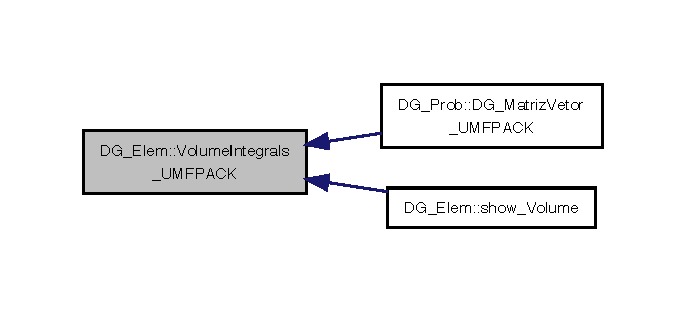
\includegraphics[width=329pt]{classDG__Elem_ab3de164caf40da7cc0b123928ad83cc9_icgraph}
\end{center}
\end{figure}
\mbox{\Hypertarget{classDG__Elem_a2a2a90dfc3c456b66f7e1890d0f236f2}\label{classDG__Elem_a2a2a90dfc3c456b66f7e1890d0f236f2}} 
\index{D\+G\+\_\+\+Elem@{D\+G\+\_\+\+Elem}!Volume\+IntegralsT@{Volume\+IntegralsT}}
\index{Volume\+IntegralsT@{Volume\+IntegralsT}!D\+G\+\_\+\+Elem@{D\+G\+\_\+\+Elem}}
\subsubsection{\texorpdfstring{Volume\+Integrals\+T()}{VolumeIntegralsT()}}
{\footnotesize\ttfamily void D\+G\+\_\+\+Elem\+::\+Volume\+IntegralsT (\begin{DoxyParamCaption}\item[{const double}]{Dt\+\_\+new,  }\item[{const double}]{Dt\+\_\+old,  }\item[{int \&}]{count,  }\item[{int $\ast$}]{Ti,  }\item[{int $\ast$}]{Tj,  }\item[{double $\ast$}]{Tx,  }\item[{double $\ast$}]{B }\end{DoxyParamCaption})}



Definition at line 960 of file D\+G\+\_\+\+Elem.\+cpp.



References aux, Stdel\+::eval\+\_\+\+Phi(), Stdel\+::eval\+G\+Q(), Ph\+Elem$<$ 2 $>$\+::gbnmap, Ph\+Elem$<$ 2 $>$\+::\+JV, m, Mass\+\_\+sn, Stdel\+::\+N\+G\+Q\+P\+\_\+val(), Ph\+Elem$<$ 2 $>$\+::numn, phi\+\_\+r, porosidade, Ph\+Elem$<$ 2 $>$\+::ptr\+\_\+stdel, sat, sn, sna, and Ph\+Elem$<$ 2 $>$\+::u0.



Referenced by show\+\_\+\+Volume().

Here is the call graph for this function\+:
\nopagebreak
\begin{figure}[H]
\begin{center}
\leavevmode
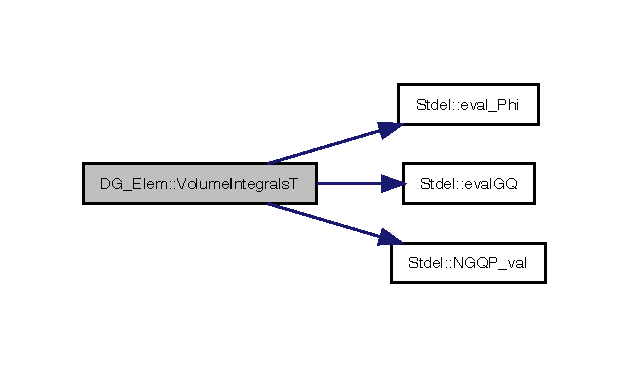
\includegraphics[width=302pt]{classDG__Elem_a2a2a90dfc3c456b66f7e1890d0f236f2_cgraph}
\end{center}
\end{figure}
Here is the caller graph for this function\+:
\nopagebreak
\begin{figure}[H]
\begin{center}
\leavevmode
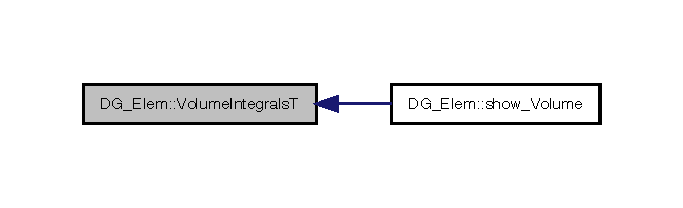
\includegraphics[width=328pt]{classDG__Elem_a2a2a90dfc3c456b66f7e1890d0f236f2_icgraph}
\end{center}
\end{figure}
\mbox{\Hypertarget{classDG__Elem_a84fab76e27b414367eb553f9d4841889}\label{classDG__Elem_a84fab76e27b414367eb553f9d4841889}} 
\index{D\+G\+\_\+\+Elem@{D\+G\+\_\+\+Elem}!Volume\+Tracos@{Volume\+Tracos}}
\index{Volume\+Tracos@{Volume\+Tracos}!D\+G\+\_\+\+Elem@{D\+G\+\_\+\+Elem}}
\subsubsection{\texorpdfstring{Volume\+Tracos()}{VolumeTracos()}}
{\footnotesize\ttfamily void D\+G\+\_\+\+Elem\+::\+Volume\+Tracos (\begin{DoxyParamCaption}\item[{const double}]{Dt,  }\item[{\hyperlink{classFluids}{Fluids}}]{fls,  }\item[{double $\ast$}]{gbtrsn = {\ttfamily NULL},  }\item[{double $\ast$}]{gbtrpw = {\ttfamily NULL} }\end{DoxyParamCaption})}



Definition at line 1024 of file D\+G\+\_\+\+Elem.\+cpp.



References aux, d2\+\_\+pc, Fluids\+::d2pc(), d\+\_\+lambdan, d\+\_\+lambdat, d\+\_\+lambdaw, d\+\_\+pc, Fluids\+::dkrn(), Fluids\+::dkrw(), Fluids\+::dpc(), Stdel\+::eval\+G\+Q(), Ph\+Elem$<$ 2 $>$\+::gbtrbmap, Stdel\+::\+Gradiente(), Ph\+Elem$<$ 2 $>$\+::\+JV, Fluids\+::\+Krn(), Fluids\+::\+Krw(), lambdan, lambdat, lambdaw, m, mun, muw, Ph\+Elem$<$ 2 $>$\+::ndim, Stdel\+::\+N\+G\+Q\+P\+\_\+val(), Ph\+Elem$<$ 2 $>$\+::numborders, pc, perm, pres, Fluids\+::pressao\+\_\+capilar(), Ph\+Elem$<$ 2 $>$\+::ptr\+\_\+stdel, Ph\+Elem$<$ 2 $>$\+::ptvert, pw, Stdel\+::qborder\+\_\+val(), qmax, sat, Fluids\+::show\+\_\+mun(), Fluids\+::show\+\_\+muw(), Ph\+Elem$<$ 2 $>$\+::sinal, sn, Stdel\+::trace(), Tr\+Kgrad\+\_\+pc, Tr\+Kgrad\+\_\+pw, Tr\+Kgrad\+\_\+sn, Trpw, Trsn, Ph\+Elem$<$ 2 $>$\+::u0, and Ph\+Elem$<$ 2 $>$\+::\+Vert\+\_\+map.



Referenced by D\+G\+\_\+\+Prob\+::\+D\+G\+\_\+imprimir\+\_\+taxas\+\_\+de\+\_\+producao(), D\+G\+\_\+\+Prob\+::\+D\+G\+\_\+\+Matriz\+Vetor\+\_\+\+Epetra(), D\+G\+\_\+\+Prob\+::\+D\+G\+\_\+\+Matriz\+Vetor\+\_\+\+U\+M\+F\+P\+A\+C\+K(), and show\+\_\+\+Volume().

Here is the call graph for this function\+:
\nopagebreak
\begin{figure}[H]
\begin{center}
\leavevmode
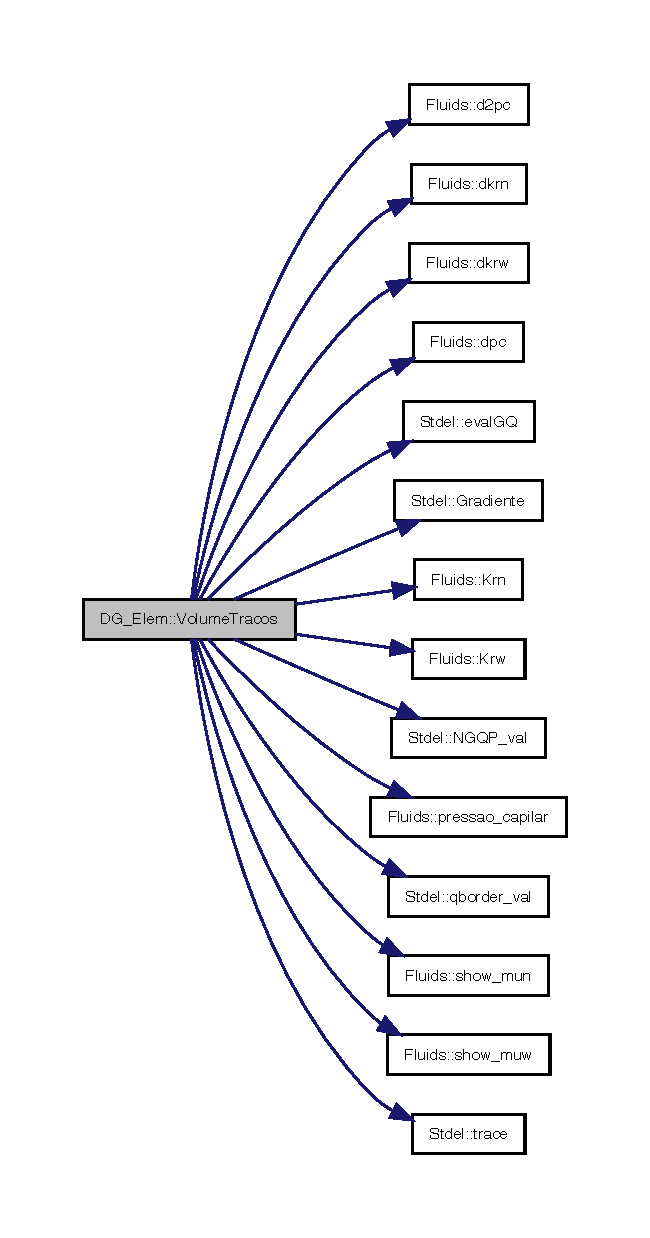
\includegraphics[height=550pt]{classDG__Elem_a84fab76e27b414367eb553f9d4841889_cgraph}
\end{center}
\end{figure}
Here is the caller graph for this function\+:
\nopagebreak
\begin{figure}[H]
\begin{center}
\leavevmode
\includegraphics[width=350pt]{classDG__Elem_a84fab76e27b414367eb553f9d4841889_icgraph}
\end{center}
\end{figure}
\mbox{\Hypertarget{classPhElem_a55ef84501df0d4e8aec6d49846e21237}\label{classPhElem_a55ef84501df0d4e8aec6d49846e21237}} 
\index{D\+G\+\_\+\+Elem@{D\+G\+\_\+\+Elem}!zera\+\_\+bs@{zera\+\_\+bs}}
\index{zera\+\_\+bs@{zera\+\_\+bs}!D\+G\+\_\+\+Elem@{D\+G\+\_\+\+Elem}}
\subsubsection{\texorpdfstring{zera\+\_\+bs()}{zera\_bs()}}
{\footnotesize\ttfamily void \hyperlink{classPhElem}{Ph\+Elem}$<$ Num\+Variaveis $>$\+::zera\+\_\+bs (\begin{DoxyParamCaption}\item[{const int \&}]{k }\end{DoxyParamCaption})\hspace{0.3cm}{\ttfamily [inherited]}}

\mbox{\Hypertarget{classPhElem_a46f2be4d83b5c7c2cc9c6699f1fe977c}\label{classPhElem_a46f2be4d83b5c7c2cc9c6699f1fe977c}} 
\index{D\+G\+\_\+\+Elem@{D\+G\+\_\+\+Elem}!zera\+\_\+vetores@{zera\+\_\+vetores}}
\index{zera\+\_\+vetores@{zera\+\_\+vetores}!D\+G\+\_\+\+Elem@{D\+G\+\_\+\+Elem}}
\subsubsection{\texorpdfstring{zera\+\_\+vetores()}{zera\_vetores()}}
{\footnotesize\ttfamily void \hyperlink{classPhElem}{Ph\+Elem}$<$ Num\+Variaveis $>$\+::zera\+\_\+vetores (\begin{DoxyParamCaption}\item[{const int \&}]{k }\end{DoxyParamCaption})\hspace{0.3cm}{\ttfamily [inherited]}}



\subsection{Member Data Documentation}
\mbox{\Hypertarget{classPhElem_a27a4f856d62b68758e4c03c09b4c37f8}\label{classPhElem_a27a4f856d62b68758e4c03c09b4c37f8}} 
\index{D\+G\+\_\+\+Elem@{D\+G\+\_\+\+Elem}!aresta\+\_\+map@{aresta\+\_\+map}}
\index{aresta\+\_\+map@{aresta\+\_\+map}!D\+G\+\_\+\+Elem@{D\+G\+\_\+\+Elem}}
\subsubsection{\texorpdfstring{aresta\+\_\+map}{aresta\_map}}
{\footnotesize\ttfamily int \hyperlink{classPhElem}{Ph\+Elem}$<$ Num\+Variaveis $>$\+::aresta\+\_\+map\mbox{[}12\mbox{]}\hspace{0.3cm}{\ttfamily [protected]}, {\ttfamily [inherited]}}



Definition at line 195 of file Ph\+Elem.\+hpp.

\mbox{\Hypertarget{classPhElem_aeaebffae27dd713bbc06ad07b7b727a3}\label{classPhElem_aeaebffae27dd713bbc06ad07b7b727a3}} 
\index{D\+G\+\_\+\+Elem@{D\+G\+\_\+\+Elem}!b0@{b0}}
\index{b0@{b0}!D\+G\+\_\+\+Elem@{D\+G\+\_\+\+Elem}}
\subsubsection{\texorpdfstring{b0}{b0}}
{\footnotesize\ttfamily double$\ast$ \hyperlink{classPhElem}{Ph\+Elem}$<$ Num\+Variaveis $>$\+::b0\mbox{[}Num\+Variaveis\mbox{]}\hspace{0.3cm}{\ttfamily [protected]}, {\ttfamily [inherited]}}



\mbox{[}M\+A\+X\+M\+O\+D\+E\+S$\ast$\+M\+A\+X\+N\+F\+I\+E\+L\+DS\mbox{]}; vector of body forces 



Definition at line 201 of file Ph\+Elem.\+hpp.

\mbox{\Hypertarget{classPhElem_ad153ce0aef191aac0f28f2addd213c71}\label{classPhElem_ad153ce0aef191aac0f28f2addd213c71}} 
\index{D\+G\+\_\+\+Elem@{D\+G\+\_\+\+Elem}!border\+\_\+num@{border\+\_\+num}}
\index{border\+\_\+num@{border\+\_\+num}!D\+G\+\_\+\+Elem@{D\+G\+\_\+\+Elem}}
\subsubsection{\texorpdfstring{border\+\_\+num}{border\_num}}
{\footnotesize\ttfamily int \hyperlink{classPhElem}{Ph\+Elem}$<$ Num\+Variaveis $>$\+::border\+\_\+num\mbox{[}12\mbox{]}\hspace{0.3cm}{\ttfamily [protected]}, {\ttfamily [inherited]}}



Definition at line 195 of file Ph\+Elem.\+hpp.



Referenced by inicia\+\_\+funcoes\+\_\+na\+\_\+borda(), and inicia\+\_\+tracos().

\mbox{\Hypertarget{classPhElem_a42b747116ec9223cdebbc424e27f4089}\label{classPhElem_a42b747116ec9223cdebbc424e27f4089}} 
\index{D\+G\+\_\+\+Elem@{D\+G\+\_\+\+Elem}!bs@{bs}}
\index{bs@{bs}!D\+G\+\_\+\+Elem@{D\+G\+\_\+\+Elem}}
\subsubsection{\texorpdfstring{bs}{bs}}
{\footnotesize\ttfamily double$\ast$ \hyperlink{classPhElem}{Ph\+Elem}$<$ Num\+Variaveis $>$\+::bs\mbox{[}Num\+Variaveis\mbox{]}\hspace{0.3cm}{\ttfamily [protected]}, {\ttfamily [inherited]}}



vector of force boundary conditions 



Definition at line 202 of file Ph\+Elem.\+hpp.

\mbox{\Hypertarget{classPhElem_a300b484c07390b9016d9ed97980d76b3}\label{classPhElem_a300b484c07390b9016d9ed97980d76b3}} 
\index{D\+G\+\_\+\+Elem@{D\+G\+\_\+\+Elem}!face\+\_\+map@{face\+\_\+map}}
\index{face\+\_\+map@{face\+\_\+map}!D\+G\+\_\+\+Elem@{D\+G\+\_\+\+Elem}}
\subsubsection{\texorpdfstring{face\+\_\+map}{face\_map}}
{\footnotesize\ttfamily int \hyperlink{classPhElem}{Ph\+Elem}$<$ Num\+Variaveis $>$\+::face\+\_\+map\mbox{[}6\mbox{]}\hspace{0.3cm}{\ttfamily [protected]}, {\ttfamily [inherited]}}



Definition at line 195 of file Ph\+Elem.\+hpp.

\mbox{\Hypertarget{classPhElem_ab27e9040a72ec923a90cffb25f5b0c15}\label{classPhElem_ab27e9040a72ec923a90cffb25f5b0c15}} 
\index{D\+G\+\_\+\+Elem@{D\+G\+\_\+\+Elem}!gbnmap@{gbnmap}}
\index{gbnmap@{gbnmap}!D\+G\+\_\+\+Elem@{D\+G\+\_\+\+Elem}}
\subsubsection{\texorpdfstring{gbnmap}{gbnmap}}
{\footnotesize\ttfamily int \hyperlink{classPhElem}{Ph\+Elem}$<$ Num\+Variaveis $>$\+::gbnmap\mbox{[}Num\+Variaveis\mbox{]}\mbox{[}\hyperlink{MyOptions_8h_a2f91e7a0b4bf68a62a0f3d38904dea2c}{M\+A\+X\+NN}\mbox{]}\hspace{0.3cm}{\ttfamily [protected]}, {\ttfamily [inherited]}}



mapping from local to global nodes (or modes) 



Definition at line 197 of file Ph\+Elem.\+hpp.



Referenced by Volume\+Integrals(), Volume\+Integrals\+\_\+\+I\+G(), Volume\+Integrals\+\_\+\+U\+M\+F\+P\+A\+C\+K(), and Volume\+Integrals\+T().

\mbox{\Hypertarget{classPhElem_a8188f64662092eb065a85d49f3ae6649}\label{classPhElem_a8188f64662092eb065a85d49f3ae6649}} 
\index{D\+G\+\_\+\+Elem@{D\+G\+\_\+\+Elem}!gbtrbmap@{gbtrbmap}}
\index{gbtrbmap@{gbtrbmap}!D\+G\+\_\+\+Elem@{D\+G\+\_\+\+Elem}}
\subsubsection{\texorpdfstring{gbtrbmap}{gbtrbmap}}
{\footnotesize\ttfamily int \hyperlink{classPhElem}{Ph\+Elem}$<$ Num\+Variaveis $>$\+::gbtrbmap\hspace{0.3cm}{\ttfamily [protected]}, {\ttfamily [inherited]}}



Beginning index on the global array where the local border Gauss quadrature points (traces) are mapped; this map facilitates the use of mpi for paralell calculations over element borders. 



Definition at line 207 of file Ph\+Elem.\+hpp.



Referenced by Volume\+Integrals(), Volume\+Integrals\+\_\+\+U\+M\+F\+P\+A\+C\+K(), and Volume\+Tracos().

\mbox{\Hypertarget{classDG__Elem_a89a6e65d3cca9d70aff0af308e1c4828}\label{classDG__Elem_a89a6e65d3cca9d70aff0af308e1c4828}} 
\index{D\+G\+\_\+\+Elem@{D\+G\+\_\+\+Elem}!Grad\+Phi@{Grad\+Phi}}
\index{Grad\+Phi@{Grad\+Phi}!D\+G\+\_\+\+Elem@{D\+G\+\_\+\+Elem}}
\subsubsection{\texorpdfstring{Grad\+Phi}{GradPhi}}
{\footnotesize\ttfamily double$\ast$$\ast$$\ast$$\ast$ D\+G\+\_\+\+Elem\+::\+Grad\+Phi\hspace{0.3cm}{\ttfamily [private]}}



Definition at line 124 of file D\+G\+\_\+\+Elem.\+hpp.



Referenced by finaliza\+\_\+vetores(), inicia\+\_\+funcoes\+\_\+na\+\_\+borda(), inicia\+\_\+tracos(), inicia\+\_\+vetores(), Volume\+Integrals(), Volume\+Integrals\+\_\+\+I\+G(), and Volume\+Integrals\+\_\+\+U\+M\+F\+P\+A\+C\+K().

\mbox{\Hypertarget{classPhElem_a27acf6bc6ac9eaf94a7cce52522b3b92}\label{classPhElem_a27acf6bc6ac9eaf94a7cce52522b3b92}} 
\index{D\+G\+\_\+\+Elem@{D\+G\+\_\+\+Elem}!J@{J}}
\index{J@{J}!D\+G\+\_\+\+Elem@{D\+G\+\_\+\+Elem}}
\subsubsection{\texorpdfstring{J}{J}}
{\footnotesize\ttfamily double \hyperlink{classPhElem}{Ph\+Elem}$<$ Num\+Variaveis $>$\+::J\hspace{0.3cm}{\ttfamily [protected]}, {\ttfamily [inherited]}}



Jacobian from the physical to the standard element. 



Definition at line 199 of file Ph\+Elem.\+hpp.

\mbox{\Hypertarget{classDG__Elem_a21966ef258f170053e616e17082516c8}\label{classDG__Elem_a21966ef258f170053e616e17082516c8}} 
\index{D\+G\+\_\+\+Elem@{D\+G\+\_\+\+Elem}!Jb@{Jb}}
\index{Jb@{Jb}!D\+G\+\_\+\+Elem@{D\+G\+\_\+\+Elem}}
\subsubsection{\texorpdfstring{Jb}{Jb}}
{\footnotesize\ttfamily double$\ast$ D\+G\+\_\+\+Elem\+::\+Jb\hspace{0.3cm}{\ttfamily [private]}}



Jacobiano nos pontos de Gauss sobre as bordas; usado na integração sobre bordas. 



Definition at line 115 of file D\+G\+\_\+\+Elem.\+hpp.



Referenced by finaliza\+\_\+vetores(), inicia\+\_\+funcoes\+\_\+na\+\_\+borda(), and inicia\+\_\+vetores().

\mbox{\Hypertarget{classPhElem_a569278e8b30ca90d0e6f920b5bba7dd5}\label{classPhElem_a569278e8b30ca90d0e6f920b5bba7dd5}} 
\index{D\+G\+\_\+\+Elem@{D\+G\+\_\+\+Elem}!JV@{JV}}
\index{JV@{JV}!D\+G\+\_\+\+Elem@{D\+G\+\_\+\+Elem}}
\subsubsection{\texorpdfstring{JV}{JV}}
{\footnotesize\ttfamily double$\ast$ \hyperlink{classPhElem}{Ph\+Elem}$<$ Num\+Variaveis $>$\+::JV\hspace{0.3cm}{\ttfamily [protected]}, {\ttfamily [inherited]}}



Ponteiro para matriz do Jacobiano nos pontos gaussianos;. 



Definition at line 200 of file Ph\+Elem.\+hpp.



Referenced by echo\+\_\+traco(), finaliza\+\_\+vetores(), inicia\+\_\+vetores(), Volume\+Integrals(), Volume\+Integrals\+\_\+\+I\+G(), Volume\+Integrals\+\_\+\+U\+M\+F\+P\+A\+C\+K(), Volume\+Integrals\+T(), and Volume\+Tracos().

\mbox{\Hypertarget{classDG__Elem_a32939229d5c3e35ef503c432975949cc}\label{classDG__Elem_a32939229d5c3e35ef503c432975949cc}} 
\index{D\+G\+\_\+\+Elem@{D\+G\+\_\+\+Elem}!Laplaciano\+Phi@{Laplaciano\+Phi}}
\index{Laplaciano\+Phi@{Laplaciano\+Phi}!D\+G\+\_\+\+Elem@{D\+G\+\_\+\+Elem}}
\subsubsection{\texorpdfstring{Laplaciano\+Phi}{LaplacianoPhi}}
{\footnotesize\ttfamily double$\ast$$\ast$$\ast$ D\+G\+\_\+\+Elem\+::\+Laplaciano\+Phi\hspace{0.3cm}{\ttfamily [private]}}



Definition at line 119 of file D\+G\+\_\+\+Elem.\+hpp.



Referenced by finaliza\+\_\+vetores(), inicia\+\_\+funcoes\+\_\+na\+\_\+borda(), and inicia\+\_\+vetores().

\mbox{\Hypertarget{classDG__Elem_a53a6e2f1c4d46714b67f131f44902fc3}\label{classDG__Elem_a53a6e2f1c4d46714b67f131f44902fc3}} 
\index{D\+G\+\_\+\+Elem@{D\+G\+\_\+\+Elem}!Mass\+\_\+sn@{Mass\+\_\+sn}}
\index{Mass\+\_\+sn@{Mass\+\_\+sn}!D\+G\+\_\+\+Elem@{D\+G\+\_\+\+Elem}}
\subsubsection{\texorpdfstring{Mass\+\_\+sn}{Mass\_sn}}
{\footnotesize\ttfamily double$\ast$$\ast$ D\+G\+\_\+\+Elem\+::\+Mass\+\_\+sn\hspace{0.3cm}{\ttfamily [private]}}



Definition at line 116 of file D\+G\+\_\+\+Elem.\+hpp.



Referenced by finaliza\+\_\+vetores(), inicia\+\_\+vetores(), and Volume\+Integrals\+T().

\mbox{\Hypertarget{classPhElem_af3ea3f4193f7d65855c3fabead6f2545}\label{classPhElem_af3ea3f4193f7d65855c3fabead6f2545}} 
\index{D\+G\+\_\+\+Elem@{D\+G\+\_\+\+Elem}!ndim@{ndim}}
\index{ndim@{ndim}!D\+G\+\_\+\+Elem@{D\+G\+\_\+\+Elem}}
\subsubsection{\texorpdfstring{ndim}{ndim}}
{\footnotesize\ttfamily int \hyperlink{classPhElem}{Ph\+Elem}$<$ Num\+Variaveis $>$\+::ndim\hspace{0.3cm}{\ttfamily [protected]}, {\ttfamily [inherited]}}



Spatial dimension. 



Definition at line 188 of file Ph\+Elem.\+hpp.



Referenced by calcula\+\_\+tracos(), echo\+\_\+traco(), finaliza\+\_\+vetores(), inicia\+\_\+funcoes\+\_\+na\+\_\+borda(), inicia\+\_\+tracos(), inicia\+\_\+vetores(), Traco\+\_\+grad\+\_\+phi(), Traco\+\_\+\+Kgrad\+\_\+pc(), Traco\+\_\+\+Kgrad\+\_\+pw(), Traco\+\_\+\+Kgrad\+\_\+sn(), Volume\+Integrals(), Volume\+Integrals\+\_\+\+I\+G(), Volume\+Integrals\+\_\+\+U\+M\+F\+P\+A\+C\+K(), and Volume\+Tracos().

\mbox{\Hypertarget{classPhElem_ad95c9f8ee7a993ccc7f9cdd08dddf5f6}\label{classPhElem_ad95c9f8ee7a993ccc7f9cdd08dddf5f6}} 
\index{D\+G\+\_\+\+Elem@{D\+G\+\_\+\+Elem}!numb@{numb}}
\index{numb@{numb}!D\+G\+\_\+\+Elem@{D\+G\+\_\+\+Elem}}
\subsubsection{\texorpdfstring{numb}{numb}}
{\footnotesize\ttfamily int \hyperlink{classPhElem}{Ph\+Elem}$<$ Num\+Variaveis $>$\+::numb\mbox{[}Num\+Variaveis\mbox{]}\hspace{0.3cm}{\ttfamily [protected]}, {\ttfamily [inherited]}}



Definition at line 194 of file Ph\+Elem.\+hpp.

\mbox{\Hypertarget{classPhElem_ad24d6fbe02539875405dd4a6cf094284}\label{classPhElem_ad24d6fbe02539875405dd4a6cf094284}} 
\index{D\+G\+\_\+\+Elem@{D\+G\+\_\+\+Elem}!numborders@{numborders}}
\index{numborders@{numborders}!D\+G\+\_\+\+Elem@{D\+G\+\_\+\+Elem}}
\subsubsection{\texorpdfstring{numborders}{numborders}}
{\footnotesize\ttfamily int \hyperlink{classPhElem}{Ph\+Elem}$<$ Num\+Variaveis $>$\+::numborders\hspace{0.3cm}{\ttfamily [protected]}, {\ttfamily [inherited]}}



Number of borders in the element. 



Definition at line 192 of file Ph\+Elem.\+hpp.



Referenced by calcula\+\_\+tracos(), echo\+\_\+traco(), finaliza\+\_\+vetores(), inicia\+\_\+funcoes\+\_\+na\+\_\+borda(), inicia\+\_\+tracos(), inicia\+\_\+vetores(), Volume\+Integrals(), Volume\+Integrals\+\_\+\+I\+G(), Volume\+Integrals\+\_\+\+U\+M\+F\+P\+A\+C\+K(), and Volume\+Tracos().

\mbox{\Hypertarget{classPhElem_a1c0c7833feba84d4ed83d172244ca3e1}\label{classPhElem_a1c0c7833feba84d4ed83d172244ca3e1}} 
\index{D\+G\+\_\+\+Elem@{D\+G\+\_\+\+Elem}!nume@{nume}}
\index{nume@{nume}!D\+G\+\_\+\+Elem@{D\+G\+\_\+\+Elem}}
\subsubsection{\texorpdfstring{nume}{nume}}
{\footnotesize\ttfamily int \hyperlink{classPhElem}{Ph\+Elem}$<$ Num\+Variaveis $>$\+::nume\hspace{0.3cm}{\ttfamily [protected]}, {\ttfamily [inherited]}}



Number of edges. 



Definition at line 190 of file Ph\+Elem.\+hpp.

\mbox{\Hypertarget{classPhElem_a85d9a8342adf9e155a533edf165a6fe3}\label{classPhElem_a85d9a8342adf9e155a533edf165a6fe3}} 
\index{D\+G\+\_\+\+Elem@{D\+G\+\_\+\+Elem}!numf@{numf}}
\index{numf@{numf}!D\+G\+\_\+\+Elem@{D\+G\+\_\+\+Elem}}
\subsubsection{\texorpdfstring{numf}{numf}}
{\footnotesize\ttfamily int \hyperlink{classPhElem}{Ph\+Elem}$<$ Num\+Variaveis $>$\+::numf\hspace{0.3cm}{\ttfamily [protected]}, {\ttfamily [inherited]}}



Number of faces. 



Definition at line 191 of file Ph\+Elem.\+hpp.

\mbox{\Hypertarget{classPhElem_a2ec71d768628a94d7fbe74be08a08ea9}\label{classPhElem_a2ec71d768628a94d7fbe74be08a08ea9}} 
\index{D\+G\+\_\+\+Elem@{D\+G\+\_\+\+Elem}!Num\+Local\+Vars@{Num\+Local\+Vars}}
\index{Num\+Local\+Vars@{Num\+Local\+Vars}!D\+G\+\_\+\+Elem@{D\+G\+\_\+\+Elem}}
\subsubsection{\texorpdfstring{Num\+Local\+Vars}{NumLocalVars}}
{\footnotesize\ttfamily int \hyperlink{classPhElem}{Ph\+Elem}$<$ Num\+Variaveis $>$\+::Num\+Local\+Vars\hspace{0.3cm}{\ttfamily [protected]}, {\ttfamily [inherited]}}



Definition at line 187 of file Ph\+Elem.\+hpp.



Referenced by echo\+\_\+traco(), inicia\+\_\+funcoes\+\_\+na\+\_\+borda(), inicia\+\_\+tracos(), and inicia\+\_\+vetores().

\mbox{\Hypertarget{classPhElem_a8e65fa4998d28b9b8db9b6fcf8999d20}\label{classPhElem_a8e65fa4998d28b9b8db9b6fcf8999d20}} 
\index{D\+G\+\_\+\+Elem@{D\+G\+\_\+\+Elem}!numn@{numn}}
\index{numn@{numn}!D\+G\+\_\+\+Elem@{D\+G\+\_\+\+Elem}}
\subsubsection{\texorpdfstring{numn}{numn}}
{\footnotesize\ttfamily int \hyperlink{classPhElem}{Ph\+Elem}$<$ Num\+Variaveis $>$\+::numn\mbox{[}Num\+Variaveis\mbox{]}\hspace{0.3cm}{\ttfamily [protected]}, {\ttfamily [inherited]}}



Definition at line 193 of file Ph\+Elem.\+hpp.



Referenced by calcula\+\_\+tracos(), echo\+\_\+traco(), finaliza\+\_\+vetores(), inicia\+\_\+funcoes\+\_\+na\+\_\+borda(), inicia\+\_\+tracos(), inicia\+\_\+vetores(), Volume\+Integrals(), Volume\+Integrals\+\_\+\+I\+G(), Volume\+Integrals\+\_\+\+U\+M\+F\+P\+A\+C\+K(), and Volume\+Integrals\+T().

\mbox{\Hypertarget{classPhElem_a67ed36925b04bf0f2d177c8d31737526}\label{classPhElem_a67ed36925b04bf0f2d177c8d31737526}} 
\index{D\+G\+\_\+\+Elem@{D\+G\+\_\+\+Elem}!numv@{numv}}
\index{numv@{numv}!D\+G\+\_\+\+Elem@{D\+G\+\_\+\+Elem}}
\subsubsection{\texorpdfstring{numv}{numv}}
{\footnotesize\ttfamily int \hyperlink{classPhElem}{Ph\+Elem}$<$ Num\+Variaveis $>$\+::numv\hspace{0.3cm}{\ttfamily [protected]}, {\ttfamily [inherited]}}



Number of vertices. 



Definition at line 189 of file Ph\+Elem.\+hpp.

\mbox{\Hypertarget{classPhElem_a141616ccadb4a17328626befc4330932}\label{classPhElem_a141616ccadb4a17328626befc4330932}} 
\index{D\+G\+\_\+\+Elem@{D\+G\+\_\+\+Elem}!part\+\_\+num@{part\+\_\+num}}
\index{part\+\_\+num@{part\+\_\+num}!D\+G\+\_\+\+Elem@{D\+G\+\_\+\+Elem}}
\subsubsection{\texorpdfstring{part\+\_\+num}{part\_num}}
{\footnotesize\ttfamily int \hyperlink{classPhElem}{Ph\+Elem}$<$ Num\+Variaveis $>$\+::part\+\_\+num\hspace{0.3cm}{\ttfamily [protected]}, {\ttfamily [inherited]}}



numero da particao a qual pertence 



Definition at line 196 of file Ph\+Elem.\+hpp.

\mbox{\Hypertarget{classDG__Elem_a4b1a31424c3c115bc5bb964c3b72be66}\label{classDG__Elem_a4b1a31424c3c115bc5bb964c3b72be66}} 
\index{D\+G\+\_\+\+Elem@{D\+G\+\_\+\+Elem}!perm@{perm}}
\index{perm@{perm}!D\+G\+\_\+\+Elem@{D\+G\+\_\+\+Elem}}
\subsubsection{\texorpdfstring{perm}{perm}}
{\footnotesize\ttfamily double D\+G\+\_\+\+Elem\+::perm\mbox{[}3\mbox{]}\hspace{0.3cm}{\ttfamily [private]}}



permeabilidades nas 3 direcoes 



Definition at line 111 of file D\+G\+\_\+\+Elem.\+hpp.



Referenced by calcula\+\_\+tracos(), inicia\+\_\+funcoes\+\_\+na\+\_\+borda(), inicia\+\_\+tracos(), perm\+\_\+val(), set\+\_\+permeabilidade(), Volume\+Integrals(), Volume\+Integrals\+\_\+\+I\+G(), Volume\+Integrals\+\_\+\+U\+M\+F\+P\+A\+C\+K(), and Volume\+Tracos().

\mbox{\Hypertarget{classDG__Elem_a79caff690ab51cd79dabbb5fd110d111}\label{classDG__Elem_a79caff690ab51cd79dabbb5fd110d111}} 
\index{D\+G\+\_\+\+Elem@{D\+G\+\_\+\+Elem}!Phi\+Array@{Phi\+Array}}
\index{Phi\+Array@{Phi\+Array}!D\+G\+\_\+\+Elem@{D\+G\+\_\+\+Elem}}
\subsubsection{\texorpdfstring{Phi\+Array}{PhiArray}}
{\footnotesize\ttfamily double$\ast$ D\+G\+\_\+\+Elem\+::\+Phi\+Array\hspace{0.3cm}{\ttfamily [private]}}



Definition at line 127 of file D\+G\+\_\+\+Elem.\+hpp.

\mbox{\Hypertarget{classDG__Elem_a0bb64698c7f238bf48da2d584965fcd0}\label{classDG__Elem_a0bb64698c7f238bf48da2d584965fcd0}} 
\index{D\+G\+\_\+\+Elem@{D\+G\+\_\+\+Elem}!porosidade@{porosidade}}
\index{porosidade@{porosidade}!D\+G\+\_\+\+Elem@{D\+G\+\_\+\+Elem}}
\subsubsection{\texorpdfstring{porosidade}{porosidade}}
{\footnotesize\ttfamily double D\+G\+\_\+\+Elem\+::porosidade\hspace{0.3cm}{\ttfamily [private]}}



Definition at line 110 of file D\+G\+\_\+\+Elem.\+hpp.



Referenced by set\+\_\+porosidade(), Volume\+Integrals(), Volume\+Integrals\+\_\+\+U\+M\+F\+P\+A\+C\+K(), and Volume\+Integrals\+T().

\mbox{\Hypertarget{classPhElem_a7b4509b90bcf92be76cd8fdb76d7385b}\label{classPhElem_a7b4509b90bcf92be76cd8fdb76d7385b}} 
\index{D\+G\+\_\+\+Elem@{D\+G\+\_\+\+Elem}!ptr\+\_\+stdel@{ptr\+\_\+stdel}}
\index{ptr\+\_\+stdel@{ptr\+\_\+stdel}!D\+G\+\_\+\+Elem@{D\+G\+\_\+\+Elem}}
\subsubsection{\texorpdfstring{ptr\+\_\+stdel}{ptr\_stdel}}
{\footnotesize\ttfamily \hyperlink{classStdel}{Stdel}$\ast$ \hyperlink{classPhElem}{Ph\+Elem}$<$ Num\+Variaveis $>$\+::ptr\+\_\+stdel\mbox{[}Num\+Variaveis\mbox{]}\hspace{0.3cm}{\ttfamily [protected]}, {\ttfamily [inherited]}}



Definition at line 184 of file Ph\+Elem.\+hpp.



Referenced by Atualizar\+\_\+valores(), calcula\+\_\+tracos(), echo\+\_\+traco(), finaliza\+\_\+vetores(), inicia\+\_\+funcoes\+\_\+na\+\_\+borda(), inicia\+\_\+tracos(), inicia\+\_\+vetores(), Traco\+\_\+grad\+\_\+phi(), Traco\+\_\+\+Kgrad\+\_\+pc(), Traco\+\_\+\+Kgrad\+\_\+phi\+\_\+n(), Traco\+\_\+\+Kgrad\+\_\+pw(), Traco\+\_\+\+Kgrad\+\_\+sn(), Traco\+\_\+phi(), Traco\+\_\+phi\+\_\+1(), Traco\+\_\+pw(), Traco\+\_\+sn(), Volume\+Integrals(), Volume\+Integrals\+\_\+\+I\+G(), Volume\+Integrals\+\_\+\+U\+M\+F\+P\+A\+C\+K(), Volume\+Integrals\+T(), and Volume\+Tracos().

\mbox{\Hypertarget{classPhElem_a92acc9f8f36991ce851df5e462425d3c}\label{classPhElem_a92acc9f8f36991ce851df5e462425d3c}} 
\index{D\+G\+\_\+\+Elem@{D\+G\+\_\+\+Elem}!ptvert@{ptvert}}
\index{ptvert@{ptvert}!D\+G\+\_\+\+Elem@{D\+G\+\_\+\+Elem}}
\subsubsection{\texorpdfstring{ptvert}{ptvert}}
{\footnotesize\ttfamily const \hyperlink{structVertice}{Vertice}$\ast$ \hyperlink{classPhElem}{Ph\+Elem}$<$ Num\+Variaveis $>$\+::ptvert\hspace{0.3cm}{\ttfamily [protected]}, {\ttfamily [inherited]}}



Definition at line 186 of file Ph\+Elem.\+hpp.



Referenced by Atualizar\+\_\+valores(), inicia\+\_\+funcoes\+\_\+na\+\_\+borda(), inicia\+\_\+tracos(), Volume\+Integrals(), Volume\+Integrals\+\_\+\+I\+G(), Volume\+Integrals\+\_\+\+U\+M\+F\+P\+A\+C\+K(), and Volume\+Tracos().

\mbox{\Hypertarget{classDG__Elem_afc53954789d7ec74b2cf2eb2be590d16}\label{classDG__Elem_afc53954789d7ec74b2cf2eb2be590d16}} 
\index{D\+G\+\_\+\+Elem@{D\+G\+\_\+\+Elem}!pwa@{pwa}}
\index{pwa@{pwa}!D\+G\+\_\+\+Elem@{D\+G\+\_\+\+Elem}}
\subsubsection{\texorpdfstring{pwa}{pwa}}
{\footnotesize\ttfamily double $\ast$ D\+G\+\_\+\+Elem\+::pwa\hspace{0.3cm}{\ttfamily [private]}}



ponteiros para os valores nos pontos de Gauss da saturacao e pressao atuais 



Definition at line 108 of file D\+G\+\_\+\+Elem.\+hpp.



Referenced by Atualizar\+\_\+valores(), finaliza\+\_\+vetores(), and inicia\+\_\+vetores().

\mbox{\Hypertarget{classDG__Elem_a769560386db7e7c3b64d440ed84156be}\label{classDG__Elem_a769560386db7e7c3b64d440ed84156be}} 
\index{D\+G\+\_\+\+Elem@{D\+G\+\_\+\+Elem}!qn@{qn}}
\index{qn@{qn}!D\+G\+\_\+\+Elem@{D\+G\+\_\+\+Elem}}
\subsubsection{\texorpdfstring{qn}{qn}}
{\footnotesize\ttfamily double D\+G\+\_\+\+Elem\+::qn\hspace{0.3cm}{\ttfamily [private]}}



Definition at line 112 of file D\+G\+\_\+\+Elem.\+hpp.



Referenced by set\+\_\+fontes(), Volume\+Integrals(), and Volume\+Integrals\+\_\+\+U\+M\+F\+P\+A\+C\+K().

\mbox{\Hypertarget{classDG__Elem_a89d2130d5e677207cb6c962dc90f79b3}\label{classDG__Elem_a89d2130d5e677207cb6c962dc90f79b3}} 
\index{D\+G\+\_\+\+Elem@{D\+G\+\_\+\+Elem}!qw@{qw}}
\index{qw@{qw}!D\+G\+\_\+\+Elem@{D\+G\+\_\+\+Elem}}
\subsubsection{\texorpdfstring{qw}{qw}}
{\footnotesize\ttfamily double D\+G\+\_\+\+Elem\+::qw\hspace{0.3cm}{\ttfamily [private]}}



Definition at line 112 of file D\+G\+\_\+\+Elem.\+hpp.



Referenced by set\+\_\+fontes(), Volume\+Integrals(), and Volume\+Integrals\+\_\+\+U\+M\+F\+P\+A\+C\+K().

\mbox{\Hypertarget{classDG__Elem_a56be853c8e67f9ee71f6b07aa99b3a58}\label{classDG__Elem_a56be853c8e67f9ee71f6b07aa99b3a58}} 
\index{D\+G\+\_\+\+Elem@{D\+G\+\_\+\+Elem}!rho@{rho}}
\index{rho@{rho}!D\+G\+\_\+\+Elem@{D\+G\+\_\+\+Elem}}
\subsubsection{\texorpdfstring{rho}{rho}}
{\footnotesize\ttfamily double D\+G\+\_\+\+Elem\+::rho\hspace{0.3cm}{\ttfamily [private]}}



densidade de massa ou porosidade 



Definition at line 109 of file D\+G\+\_\+\+Elem.\+hpp.



Referenced by D\+G\+\_\+\+Elem(), set\+\_\+mass\+\_\+density(), and show\+\_\+rho().

\mbox{\Hypertarget{classPhElem_a5bb9ccd4ccebf12ff0937d807c443caf}\label{classPhElem_a5bb9ccd4ccebf12ff0937d807c443caf}} 
\index{D\+G\+\_\+\+Elem@{D\+G\+\_\+\+Elem}!sgn@{sgn}}
\index{sgn@{sgn}!D\+G\+\_\+\+Elem@{D\+G\+\_\+\+Elem}}
\subsubsection{\texorpdfstring{sgn}{sgn}}
{\footnotesize\ttfamily int \hyperlink{classPhElem}{Ph\+Elem}$<$ Num\+Variaveis $>$\+::sgn\mbox{[}Num\+Variaveis\mbox{]}\mbox{[}\hyperlink{MyOptions_8h_a2f91e7a0b4bf68a62a0f3d38904dea2c}{M\+A\+X\+NN}\mbox{]}\hspace{0.3cm}{\ttfamily [protected]}, {\ttfamily [inherited]}}



sign of the local mode (or mode) 



Definition at line 198 of file Ph\+Elem.\+hpp.

\mbox{\Hypertarget{classPhElem_a4034b9b2a458d1277ca74e4e8a49627e}\label{classPhElem_a4034b9b2a458d1277ca74e4e8a49627e}} 
\index{D\+G\+\_\+\+Elem@{D\+G\+\_\+\+Elem}!sinal@{sinal}}
\index{sinal@{sinal}!D\+G\+\_\+\+Elem@{D\+G\+\_\+\+Elem}}
\subsubsection{\texorpdfstring{sinal}{sinal}}
{\footnotesize\ttfamily int \hyperlink{classPhElem}{Ph\+Elem}$<$ Num\+Variaveis $>$\+::sinal\mbox{[}12\mbox{]}\hspace{0.3cm}{\ttfamily [protected]}, {\ttfamily [inherited]}}



sinal refers to the borders 



Definition at line 195 of file Ph\+Elem.\+hpp.



Referenced by echo\+\_\+traco(), inicia\+\_\+funcoes\+\_\+na\+\_\+borda(), inicia\+\_\+tracos(), Volume\+Integrals(), Volume\+Integrals\+\_\+\+I\+G(), Volume\+Integrals\+\_\+\+U\+M\+F\+P\+A\+C\+K(), and Volume\+Tracos().

\mbox{\Hypertarget{classDG__Elem_ac036921322e2a7d3648723ae77592af5}\label{classDG__Elem_ac036921322e2a7d3648723ae77592af5}} 
\index{D\+G\+\_\+\+Elem@{D\+G\+\_\+\+Elem}!sna@{sna}}
\index{sna@{sna}!D\+G\+\_\+\+Elem@{D\+G\+\_\+\+Elem}}
\subsubsection{\texorpdfstring{sna}{sna}}
{\footnotesize\ttfamily double$\ast$ D\+G\+\_\+\+Elem\+::sna\hspace{0.3cm}{\ttfamily [private]}}



Definition at line 108 of file D\+G\+\_\+\+Elem.\+hpp.



Referenced by Atualizar\+\_\+valores(), finaliza\+\_\+vetores(), inicia\+\_\+vetores(), Volume\+Integrals(), Volume\+Integrals\+\_\+\+U\+M\+F\+P\+A\+C\+K(), and Volume\+Integrals\+T().

\mbox{\Hypertarget{classPhElem_aebcf76eedfef93aef801fa3cab9c2708}\label{classPhElem_aebcf76eedfef93aef801fa3cab9c2708}} 
\index{D\+G\+\_\+\+Elem@{D\+G\+\_\+\+Elem}!stgbtrbmapM@{stgbtrbmapM}}
\index{stgbtrbmapM@{stgbtrbmapM}!D\+G\+\_\+\+Elem@{D\+G\+\_\+\+Elem}}
\subsubsection{\texorpdfstring{stgbtrbmapM}{stgbtrbmapM}}
{\footnotesize\ttfamily int$\ast$ \hyperlink{classPhElem}{Ph\+Elem}$<$ Num\+Variaveis $>$\+::stgbtrbmapM\hspace{0.3cm}{\ttfamily [protected]}, {\ttfamily [inherited]}}



Array containing the start point in the global trace array of the internal trace of the border. 



Definition at line 212 of file Ph\+Elem.\+hpp.



Referenced by finaliza\+\_\+vetores().

\mbox{\Hypertarget{classPhElem_a6b38afded290e7a4cfb4a215a7ebec4e}\label{classPhElem_a6b38afded290e7a4cfb4a215a7ebec4e}} 
\index{D\+G\+\_\+\+Elem@{D\+G\+\_\+\+Elem}!stgbtrbmapP@{stgbtrbmapP}}
\index{stgbtrbmapP@{stgbtrbmapP}!D\+G\+\_\+\+Elem@{D\+G\+\_\+\+Elem}}
\subsubsection{\texorpdfstring{stgbtrbmapP}{stgbtrbmapP}}
{\footnotesize\ttfamily int$\ast$ \hyperlink{classPhElem}{Ph\+Elem}$<$ Num\+Variaveis $>$\+::stgbtrbmapP\hspace{0.3cm}{\ttfamily [protected]}, {\ttfamily [inherited]}}



Array containing the start point in the global trace array of the external trace of the border. 



Definition at line 214 of file Ph\+Elem.\+hpp.



Referenced by finaliza\+\_\+vetores().

\mbox{\Hypertarget{classDG__Elem_acb3ed0d11e27ceae8f0f7c33496aa7e8}\label{classDG__Elem_acb3ed0d11e27ceae8f0f7c33496aa7e8}} 
\index{D\+G\+\_\+\+Elem@{D\+G\+\_\+\+Elem}!Tr\+Grad\+Phi@{Tr\+Grad\+Phi}}
\index{Tr\+Grad\+Phi@{Tr\+Grad\+Phi}!D\+G\+\_\+\+Elem@{D\+G\+\_\+\+Elem}}
\subsubsection{\texorpdfstring{Tr\+Grad\+Phi}{TrGradPhi}}
{\footnotesize\ttfamily double$\ast$$\ast$$\ast$$\ast$$\ast$ D\+G\+\_\+\+Elem\+::\+Tr\+Grad\+Phi\hspace{0.3cm}{\ttfamily [private]}}



Definition at line 126 of file D\+G\+\_\+\+Elem.\+hpp.



Referenced by calcula\+\_\+tracos(), echo\+\_\+traco(), finaliza\+\_\+vetores(), inicia\+\_\+funcoes\+\_\+na\+\_\+borda(), inicia\+\_\+tracos(), inicia\+\_\+vetores(), and Traco\+\_\+grad\+\_\+phi().

\mbox{\Hypertarget{classDG__Elem_a57dac9aed0b175230089be51335e2dfa}\label{classDG__Elem_a57dac9aed0b175230089be51335e2dfa}} 
\index{D\+G\+\_\+\+Elem@{D\+G\+\_\+\+Elem}!Tr\+Kgrad\+\_\+pc@{Tr\+Kgrad\+\_\+pc}}
\index{Tr\+Kgrad\+\_\+pc@{Tr\+Kgrad\+\_\+pc}!D\+G\+\_\+\+Elem@{D\+G\+\_\+\+Elem}}
\subsubsection{\texorpdfstring{Tr\+Kgrad\+\_\+pc}{TrKgrad\_pc}}
{\footnotesize\ttfamily double$\ast$$\ast$$\ast$ D\+G\+\_\+\+Elem\+::\+Tr\+Kgrad\+\_\+pc\hspace{0.3cm}{\ttfamily [private]}}



Definition at line 122 of file D\+G\+\_\+\+Elem.\+hpp.



Referenced by calcula\+\_\+tracos(), finaliza\+\_\+vetores(), inicia\+\_\+vetores(), Traco\+\_\+\+Kgrad\+\_\+pc(), Volume\+Integrals(), Volume\+Integrals\+\_\+\+I\+G(), Volume\+Integrals\+\_\+\+U\+M\+F\+P\+A\+C\+K(), and Volume\+Tracos().

\mbox{\Hypertarget{classDG__Elem_a9c510976b9964cc09f695b5c1becbc2e}\label{classDG__Elem_a9c510976b9964cc09f695b5c1becbc2e}} 
\index{D\+G\+\_\+\+Elem@{D\+G\+\_\+\+Elem}!Tr\+Kgrad\+\_\+pw@{Tr\+Kgrad\+\_\+pw}}
\index{Tr\+Kgrad\+\_\+pw@{Tr\+Kgrad\+\_\+pw}!D\+G\+\_\+\+Elem@{D\+G\+\_\+\+Elem}}
\subsubsection{\texorpdfstring{Tr\+Kgrad\+\_\+pw}{TrKgrad\_pw}}
{\footnotesize\ttfamily double$\ast$$\ast$$\ast$ D\+G\+\_\+\+Elem\+::\+Tr\+Kgrad\+\_\+pw\hspace{0.3cm}{\ttfamily [private]}}



Definition at line 121 of file D\+G\+\_\+\+Elem.\+hpp.



Referenced by calcula\+\_\+tracos(), finaliza\+\_\+vetores(), inicia\+\_\+vetores(), Traco\+\_\+\+Kgrad\+\_\+pw(), Volume\+Integrals(), Volume\+Integrals\+\_\+\+I\+G(), Volume\+Integrals\+\_\+\+U\+M\+F\+P\+A\+C\+K(), and Volume\+Tracos().

\mbox{\Hypertarget{classDG__Elem_aa71a1b860606c8560d0ef2a981580340}\label{classDG__Elem_aa71a1b860606c8560d0ef2a981580340}} 
\index{D\+G\+\_\+\+Elem@{D\+G\+\_\+\+Elem}!Tr\+Kgrad\+\_\+sn@{Tr\+Kgrad\+\_\+sn}}
\index{Tr\+Kgrad\+\_\+sn@{Tr\+Kgrad\+\_\+sn}!D\+G\+\_\+\+Elem@{D\+G\+\_\+\+Elem}}
\subsubsection{\texorpdfstring{Tr\+Kgrad\+\_\+sn}{TrKgrad\_sn}}
{\footnotesize\ttfamily double$\ast$$\ast$$\ast$ D\+G\+\_\+\+Elem\+::\+Tr\+Kgrad\+\_\+sn\hspace{0.3cm}{\ttfamily [private]}}



Definition at line 120 of file D\+G\+\_\+\+Elem.\+hpp.



Referenced by calcula\+\_\+tracos(), finaliza\+\_\+vetores(), inicia\+\_\+vetores(), Traco\+\_\+\+Kgrad\+\_\+sn(), Volume\+Integrals(), Volume\+Integrals\+\_\+\+I\+G(), Volume\+Integrals\+\_\+\+U\+M\+F\+P\+A\+C\+K(), and Volume\+Tracos().

\mbox{\Hypertarget{classDG__Elem_a2703c18a4eb102761f135b01958110c6}\label{classDG__Elem_a2703c18a4eb102761f135b01958110c6}} 
\index{D\+G\+\_\+\+Elem@{D\+G\+\_\+\+Elem}!Tr\+Kgrad\+Phi\+\_\+n@{Tr\+Kgrad\+Phi\+\_\+n}}
\index{Tr\+Kgrad\+Phi\+\_\+n@{Tr\+Kgrad\+Phi\+\_\+n}!D\+G\+\_\+\+Elem@{D\+G\+\_\+\+Elem}}
\subsubsection{\texorpdfstring{Tr\+Kgrad\+Phi\+\_\+n}{TrKgradPhi\_n}}
{\footnotesize\ttfamily double$\ast$$\ast$$\ast$$\ast$ D\+G\+\_\+\+Elem\+::\+Tr\+Kgrad\+Phi\+\_\+n\hspace{0.3cm}{\ttfamily [private]}}



Definition at line 125 of file D\+G\+\_\+\+Elem.\+hpp.



Referenced by echo\+\_\+traco(), finaliza\+\_\+vetores(), inicia\+\_\+funcoes\+\_\+na\+\_\+borda(), inicia\+\_\+tracos(), inicia\+\_\+vetores(), and Traco\+\_\+\+Kgrad\+\_\+phi\+\_\+n().

\mbox{\Hypertarget{classDG__Elem_ae1432d30cbd7b063fc859a65362ee8bf}\label{classDG__Elem_ae1432d30cbd7b063fc859a65362ee8bf}} 
\index{D\+G\+\_\+\+Elem@{D\+G\+\_\+\+Elem}!Tr\+Phi@{Tr\+Phi}}
\index{Tr\+Phi@{Tr\+Phi}!D\+G\+\_\+\+Elem@{D\+G\+\_\+\+Elem}}
\subsubsection{\texorpdfstring{Tr\+Phi}{TrPhi}}
{\footnotesize\ttfamily double$\ast$$\ast$$\ast$$\ast$ D\+G\+\_\+\+Elem\+::\+Tr\+Phi\hspace{0.3cm}{\ttfamily [private]}}



Definition at line 123 of file D\+G\+\_\+\+Elem.\+hpp.



Referenced by calcula\+\_\+tracos(), echo\+\_\+traco(), finaliza\+\_\+vetores(), inicia\+\_\+funcoes\+\_\+na\+\_\+borda(), inicia\+\_\+tracos(), inicia\+\_\+vetores(), Traco\+\_\+phi(), and Traco\+\_\+phi\+\_\+1().

\mbox{\Hypertarget{classDG__Elem_a77316e95196e96ce7b612334075c8307}\label{classDG__Elem_a77316e95196e96ce7b612334075c8307}} 
\index{D\+G\+\_\+\+Elem@{D\+G\+\_\+\+Elem}!Trpw@{Trpw}}
\index{Trpw@{Trpw}!D\+G\+\_\+\+Elem@{D\+G\+\_\+\+Elem}}
\subsubsection{\texorpdfstring{Trpw}{Trpw}}
{\footnotesize\ttfamily double$\ast$$\ast$ D\+G\+\_\+\+Elem\+::\+Trpw\hspace{0.3cm}{\ttfamily [private]}}



Definition at line 118 of file D\+G\+\_\+\+Elem.\+hpp.



Referenced by calcula\+\_\+tracos(), finaliza\+\_\+vetores(), inicia\+\_\+vetores(), Traco\+\_\+pw(), Volume\+Integrals(), Volume\+Integrals\+\_\+\+I\+G(), Volume\+Integrals\+\_\+\+U\+M\+F\+P\+A\+C\+K(), and Volume\+Tracos().

\mbox{\Hypertarget{classDG__Elem_a57d06772c710267516e58be078a6635b}\label{classDG__Elem_a57d06772c710267516e58be078a6635b}} 
\index{D\+G\+\_\+\+Elem@{D\+G\+\_\+\+Elem}!Trsn@{Trsn}}
\index{Trsn@{Trsn}!D\+G\+\_\+\+Elem@{D\+G\+\_\+\+Elem}}
\subsubsection{\texorpdfstring{Trsn}{Trsn}}
{\footnotesize\ttfamily double$\ast$$\ast$ D\+G\+\_\+\+Elem\+::\+Trsn\hspace{0.3cm}{\ttfamily [private]}}



Definition at line 117 of file D\+G\+\_\+\+Elem.\+hpp.



Referenced by calcula\+\_\+tracos(), finaliza\+\_\+vetores(), inicia\+\_\+vetores(), Traco\+\_\+sn(), Volume\+Integrals(), Volume\+Integrals\+\_\+\+I\+G(), Volume\+Integrals\+\_\+\+U\+M\+F\+P\+A\+C\+K(), and Volume\+Tracos().

\mbox{\Hypertarget{classPhElem_a1ed1b45136a718afef64c846fb905546}\label{classPhElem_a1ed1b45136a718afef64c846fb905546}} 
\index{D\+G\+\_\+\+Elem@{D\+G\+\_\+\+Elem}!type@{type}}
\index{type@{type}!D\+G\+\_\+\+Elem@{D\+G\+\_\+\+Elem}}
\subsubsection{\texorpdfstring{type}{type}}
{\footnotesize\ttfamily int \hyperlink{classPhElem}{Ph\+Elem}$<$ Num\+Variaveis $>$\+::type\hspace{0.3cm}{\ttfamily [protected]}, {\ttfamily [inherited]}}



Definition at line 185 of file Ph\+Elem.\+hpp.

\mbox{\Hypertarget{classPhElem_a560dc47ac8a684d84b05851ce52e044b}\label{classPhElem_a560dc47ac8a684d84b05851ce52e044b}} 
\index{D\+G\+\_\+\+Elem@{D\+G\+\_\+\+Elem}!u0@{u0}}
\index{u0@{u0}!D\+G\+\_\+\+Elem@{D\+G\+\_\+\+Elem}}
\subsubsection{\texorpdfstring{u0}{u0}}
{\footnotesize\ttfamily double$\ast$ \hyperlink{classPhElem}{Ph\+Elem}$<$ Num\+Variaveis $>$\+::u0\mbox{[}Num\+Variaveis\mbox{]}\hspace{0.3cm}{\ttfamily [protected]}, {\ttfamily [inherited]}}



vector with the coefficients of each mode 



Definition at line 203 of file Ph\+Elem.\+hpp.



Referenced by Atualizar\+\_\+valores(), calcula\+\_\+tracos(), finaliza\+\_\+vetores(), inicia\+\_\+vetores(), Volume\+Integrals(), Volume\+Integrals\+\_\+\+I\+G(), Volume\+Integrals\+\_\+\+U\+M\+F\+P\+A\+C\+K(), Volume\+Integrals\+T(), and Volume\+Tracos().

\mbox{\Hypertarget{classPhElem_a98781f3744597bad01eff75b31734d4b}\label{classPhElem_a98781f3744597bad01eff75b31734d4b}} 
\index{D\+G\+\_\+\+Elem@{D\+G\+\_\+\+Elem}!usave@{usave}}
\index{usave@{usave}!D\+G\+\_\+\+Elem@{D\+G\+\_\+\+Elem}}
\subsubsection{\texorpdfstring{usave}{usave}}
{\footnotesize\ttfamily double$\ast$ \hyperlink{classPhElem}{Ph\+Elem}$<$ Num\+Variaveis $>$\+::usave\mbox{[}Num\+Variaveis\mbox{]}\hspace{0.3cm}{\ttfamily [protected]}, {\ttfamily [inherited]}}



Definition at line 204 of file Ph\+Elem.\+hpp.



Referenced by finaliza\+\_\+vetores(), and inicia\+\_\+vetores().

\mbox{\Hypertarget{classPhElem_a07f19f862b13cc9c5f80271b03a5a023}\label{classPhElem_a07f19f862b13cc9c5f80271b03a5a023}} 
\index{D\+G\+\_\+\+Elem@{D\+G\+\_\+\+Elem}!Vert\+\_\+map@{Vert\+\_\+map}}
\index{Vert\+\_\+map@{Vert\+\_\+map}!D\+G\+\_\+\+Elem@{D\+G\+\_\+\+Elem}}
\subsubsection{\texorpdfstring{Vert\+\_\+map}{Vert\_map}}
{\footnotesize\ttfamily int \hyperlink{classPhElem}{Ph\+Elem}$<$ Num\+Variaveis $>$\+::Vert\+\_\+map\mbox{[}8\mbox{]}\hspace{0.3cm}{\ttfamily [protected]}, {\ttfamily [inherited]}}



Definition at line 195 of file Ph\+Elem.\+hpp.



Referenced by Atualizar\+\_\+valores(), inicia\+\_\+funcoes\+\_\+na\+\_\+borda(), inicia\+\_\+tracos(), Volume\+Integrals(), Volume\+Integrals\+\_\+\+I\+G(), Volume\+Integrals\+\_\+\+U\+M\+F\+P\+A\+C\+K(), and Volume\+Tracos().

\mbox{\Hypertarget{classPhElem_a65f545dc1bf0d90240419934eb711a9d}\label{classPhElem_a65f545dc1bf0d90240419934eb711a9d}} 
\index{D\+G\+\_\+\+Elem@{D\+G\+\_\+\+Elem}!vetores\+\_\+iniciados@{vetores\+\_\+iniciados}}
\index{vetores\+\_\+iniciados@{vetores\+\_\+iniciados}!D\+G\+\_\+\+Elem@{D\+G\+\_\+\+Elem}}
\subsubsection{\texorpdfstring{vetores\+\_\+iniciados}{vetores\_iniciados}}
{\footnotesize\ttfamily int \hyperlink{classPhElem}{Ph\+Elem}$<$ Num\+Variaveis $>$\+::vetores\+\_\+iniciados\hspace{0.3cm}{\ttfamily [protected]}, {\ttfamily [inherited]}}



Definition at line 216 of file Ph\+Elem.\+hpp.



Referenced by D\+G\+\_\+\+Elem(), finaliza\+\_\+vetores(), and inicia\+\_\+vetores().

\mbox{\Hypertarget{classDG__Elem_aeb8874934ea534afbee1017456e54051}\label{classDG__Elem_aeb8874934ea534afbee1017456e54051}} 
\index{D\+G\+\_\+\+Elem@{D\+G\+\_\+\+Elem}!Volume@{Volume}}
\index{Volume@{Volume}!D\+G\+\_\+\+Elem@{D\+G\+\_\+\+Elem}}
\subsubsection{\texorpdfstring{Volume}{Volume}}
{\footnotesize\ttfamily double D\+G\+\_\+\+Elem\+::\+Volume\hspace{0.3cm}{\ttfamily [private]}}



Volume do elemento ( = area do elemento para elementos bidimensionais e comprimento para elem. 1D. 



Definition at line 113 of file D\+G\+\_\+\+Elem.\+hpp.



Referenced by show\+\_\+\+Volume().



The documentation for this class was generated from the following files\+:\begin{DoxyCompactItemize}
\item 
\hyperlink{DG__Elem_8hpp}{D\+G\+\_\+\+Elem.\+hpp}\item 
\hyperlink{DG__Elem_8cpp}{D\+G\+\_\+\+Elem.\+cpp}\end{DoxyCompactItemize}

\hypertarget{classDG__Prob}{}\section{D\+G\+\_\+\+Prob Class Reference}
\label{classDG__Prob}\index{D\+G\+\_\+\+Prob@{D\+G\+\_\+\+Prob}}


{\ttfamily \#include $<$D\+G\+\_\+\+Prob.\+h$>$}



Inheritance diagram for D\+G\+\_\+\+Prob\+:
\nopagebreak
\begin{figure}[H]
\begin{center}
\leavevmode
\includegraphics[width=189pt]{classDG__Prob__inherit__graph}
\end{center}
\end{figure}


Collaboration diagram for D\+G\+\_\+\+Prob\+:
\nopagebreak
\begin{figure}[H]
\begin{center}
\leavevmode
\includegraphics[width=350pt]{classDG__Prob__coll__graph}
\end{center}
\end{figure}
\subsection*{Public Member Functions}
\begin{DoxyCompactItemize}
\item 
\hyperlink{classDG__Prob_aaa40b75df07b3580d72d012d3e16649e}{D\+G\+\_\+\+Prob} (Epetra\+\_\+\+Comm \&comm)
\item 
\hyperlink{classDG__Prob_ac7d67077fa8154c22a52d63a24db7fba}{$\sim$\+D\+G\+\_\+\+Prob} ()
\item 
void \hyperlink{classDG__Prob_a43fca83a2395515cd1c0c3083463532d}{preamble} (char $\ast$str)
\item 
void \hyperlink{classDG__Prob_a015d792341ee05b1b3eaef7990bf1e06}{Driver} (char $\ast$argv=0)
\item 
void \hyperlink{classDG__Prob_a646bbb0fd2786395486c09b1aa6b2653}{D\+G\+\_\+alocar\+\_\+mem\+\_\+local} (const int \hyperlink{DG__EI__Header_8h_ae7d322bf04f258ba21ba82aed62c1895}{qmax}, const int \hyperlink{DG__EI__Header_8h_af01d48e9515a349111be3909b9ff2a81}{nsat}, const int \hyperlink{DG__EI__Header_8h_ab47785cba577090bf34c319609e1a039}{npres})
\item 
void \hyperlink{classDG__Prob_a06e10d482a426f07f66be721dbc4bb88}{D\+G\+\_\+liberar\+\_\+mem\+\_\+local} (const int \hyperlink{DG__EI__Header_8h_af01d48e9515a349111be3909b9ff2a81}{nsat}, const int \hyperlink{DG__EI__Header_8h_ab47785cba577090bf34c319609e1a039}{npres})
\item 
void \hyperlink{classDG__Prob_a8241ca6884495f863179ea86129b055e}{D\+G\+\_\+initial\+\_\+conditions} ()
\item 
void \hyperlink{classDG__Prob_a88ea70f33384c520034fab83e7db8e7e}{D\+G\+\_\+eco} ()
\item 
void \hyperlink{classDG__Prob_ac4dfaa4ea6466833ecb5cc5c3fcb3875}{D\+G\+\_\+\+Iterate} ()
\item 
void \hyperlink{classDG__Prob_af49f46574209aa53e1f2b3529f6a09fb}{D\+G\+\_\+\+Iterate\+\_\+\+N\+OX} ()
\item 
void \hyperlink{classDG__Prob_a4874e2992ccde1658a6ab46bc595779f}{Ge\+\_\+\+M\+V\+R\+A0} (const double \hyperlink{classDG__Prob_ad4de8afc3624f6559222e8f1f10fce6f}{Dt}, Epetra\+\_\+\+Map Map, double \&valor0, double\+\_\+t \&norm\+\_\+delta\+\_\+X)
\item 
void \hyperlink{classDG__Prob_af4fefe289d5d1beb69636817eb9f9703}{Ge\+\_\+\+M\+V\+RA} (const double \hyperlink{classDG__Prob_ad4de8afc3624f6559222e8f1f10fce6f}{Dt}, Epetra\+\_\+\+Map Map, double \&valor, int \&token, double\+\_\+t \&norm\+\_\+delta\+\_\+X)
\item 
int \hyperlink{classDG__Prob_a23d58d1583859acafd9a6d5888424374}{Eigenvectors} (const double \hyperlink{classDG__Prob_ad4de8afc3624f6559222e8f1f10fce6f}{Dt}, const Epetra\+\_\+\+Map \&Map)
\item 
void \hyperlink{classDG__Prob_acb4b2ec3201e22d62bcf50b947b10dc5}{D\+G\+\_\+condition\+Number} (Epetra\+\_\+\+Map Map)
\item 
void \hyperlink{classDG__Prob_ab28a5690b7fc91e44fe435107a4076ae}{Ler\+\_\+\+Arquivo\+\_\+\+Dados\+\_\+\+DG} (char $\ast$arq\+\_\+par)
\item 
void \hyperlink{classDG__Prob_a6941d468eec44d02bfd3f2eaedf661dc}{M\+P\+I\+\_\+\+Recebe\+\_\+\+Dados\+\_\+\+DG} ()
\item 
void \hyperlink{classDG__Prob_a6ccc7a5921dd48f971da35e5632a0b7e}{D\+G\+\_\+\+Transfere\+\_\+rst} (int $\ast$b\+\_\+in, double $\ast$b\+\_\+do, double $\ast$buff)
\item 
void \hyperlink{classDG__Prob_a2e99df149cf01faccb484389f8627d33}{D\+G\+\_\+\+Matriz\+Vetor\+\_\+\+U\+M\+F\+P\+A\+CK} (const double \hyperlink{classDG__Prob_ad4de8afc3624f6559222e8f1f10fce6f}{Dt}, int \&\hyperlink{classDG__Prob_a638611f0f0a04508f43ac7554bc8c7e2}{count}, const int \hyperlink{classDG__Prob_a18aa37594c06d6a879fad8d06f1950d1}{nz}, int $\ast$Ti, int $\ast$Tj, double $\ast$Tx, double $\ast$\hyperlink{ASPFunctions_8cpp_a57d673f8d6833fb7a7aced326df10ca9}{B})
\item 
void \hyperlink{classDG__Prob_a68ffd2ab09f51c7b29b88b006fbc5c49}{D\+G\+\_\+\+Matriz\+Vetor\+\_\+\+Epetra} (const double \hyperlink{classDG__Prob_ad4de8afc3624f6559222e8f1f10fce6f}{Dt}, Teuchos\+::\+R\+CP$<$ Epetra\+\_\+\+F\+E\+Crs\+Matrix $>$ A, Teuchos\+::\+R\+CP$<$ Epetra\+\_\+\+F\+E\+Vector $>$ R\+HS)
\item 
void \hyperlink{classDG__Prob_a862dcc9991b9091de30323b1d2b1c5a5}{D\+G\+\_\+\+E\+I\+\_\+\+Interior} (const \hyperlink{structEDGE}{E\+D\+GE} \hyperlink{classGeProb_a6c144ac05b601c5d6141c711edaaa775}{border}, int \&\hyperlink{classDG__Prob_a638611f0f0a04508f43ac7554bc8c7e2}{count}, int $\ast$Ti, int $\ast$Tj, double $\ast$Tx, double $\ast$\hyperlink{ASPFunctions_8cpp_a57d673f8d6833fb7a7aced326df10ca9}{B})
\item 
void \hyperlink{classDG__Prob_a6e6d838559f53cff2a917c3e9a5111ba}{D\+G\+\_\+\+E\+I\+\_\+\+Inflow} (const \hyperlink{structEDGE}{E\+D\+GE} \hyperlink{classGeProb_a6c144ac05b601c5d6141c711edaaa775}{border}, int \&\hyperlink{classDG__Prob_a638611f0f0a04508f43ac7554bc8c7e2}{count}, int $\ast$Ti, int $\ast$Tj, double $\ast$Tx, double $\ast$\hyperlink{ASPFunctions_8cpp_a57d673f8d6833fb7a7aced326df10ca9}{B})
\item 
void \hyperlink{classDG__Prob_a5aa1654fb60cabf97719e65ba9302cf4}{D\+G\+\_\+\+E\+I\+\_\+\+Outflow} (const \hyperlink{structEDGE}{E\+D\+GE} \hyperlink{classGeProb_a6c144ac05b601c5d6141c711edaaa775}{border}, int \&\hyperlink{classDG__Prob_a638611f0f0a04508f43ac7554bc8c7e2}{count}, int $\ast$Ti, int $\ast$Tj, double $\ast$Tx, double $\ast$\hyperlink{ASPFunctions_8cpp_a57d673f8d6833fb7a7aced326df10ca9}{B})
\item 
void \hyperlink{classDG__Prob_aa09b19ad56db0010779b0787d0edd2a5}{D\+G\+\_\+\+E\+I\+\_\+\+Epetra\+\_\+\+Interior} (const \hyperlink{structEDGE}{E\+D\+GE} \hyperlink{classGeProb_a6c144ac05b601c5d6141c711edaaa775}{border}, Teuchos\+::\+R\+CP$<$ Epetra\+\_\+\+F\+E\+Crs\+Matrix $>$ A, Teuchos\+::\+R\+CP$<$ Epetra\+\_\+\+F\+E\+Vector $>$ R\+HS)
\item 
void \hyperlink{classDG__Prob_a0c085b8fc3c827c37aa8733a2842a97f}{D\+G\+\_\+\+E\+I\+\_\+\+Epetra\+\_\+\+Inflow} (const \hyperlink{structEDGE}{E\+D\+GE} \hyperlink{classGeProb_a6c144ac05b601c5d6141c711edaaa775}{border}, Teuchos\+::\+R\+CP$<$ Epetra\+\_\+\+F\+E\+Crs\+Matrix $>$ A, Teuchos\+::\+R\+CP$<$ Epetra\+\_\+\+F\+E\+Vector $>$ R\+HS)
\item 
void \hyperlink{classDG__Prob_a7fa0c815d5707dbf3858feb3977f5ee5}{D\+G\+\_\+\+E\+I\+\_\+\+Epetra\+\_\+\+Outflow} (const \hyperlink{structEDGE}{E\+D\+GE} \hyperlink{classGeProb_a6c144ac05b601c5d6141c711edaaa775}{border}, Teuchos\+::\+R\+CP$<$ Epetra\+\_\+\+F\+E\+Crs\+Matrix $>$ A, Teuchos\+::\+R\+CP$<$ Epetra\+\_\+\+F\+E\+Vector $>$ R\+HS)
\item 
int \hyperlink{classDG__Prob_ae722c0b7a7d1bccc9dbc9d2333754b42}{D\+G\+\_\+\+E\+I\+\_\+\+Inflow} (const \hyperlink{structEDGE}{E\+D\+GE} \hyperlink{classGeProb_a6c144ac05b601c5d6141c711edaaa775}{border}, double $\ast$mx, double $\ast$\hyperlink{ASPFunctions_8cpp_a57d673f8d6833fb7a7aced326df10ca9}{B}, int $\ast$indx)
\item 
int \hyperlink{classDG__Prob_ac3054c910c2a6465c71f208b0e2b79ff}{D\+G\+\_\+\+E\+I\+\_\+\+Interior} (const \hyperlink{structEDGE}{E\+D\+GE} \hyperlink{classGeProb_a6c144ac05b601c5d6141c711edaaa775}{border}, double $\ast$mx, double $\ast$\hyperlink{ASPFunctions_8cpp_a57d673f8d6833fb7a7aced326df10ca9}{B}, int $\ast$indx)
\item 
int \hyperlink{classDG__Prob_a3e99ae33818db46884cd2683c741f36c}{D\+G\+\_\+\+E\+I\+\_\+\+Outflow} (const \hyperlink{structEDGE}{E\+D\+GE} \hyperlink{classGeProb_a6c144ac05b601c5d6141c711edaaa775}{border}, double $\ast$mx, double $\ast$\hyperlink{ASPFunctions_8cpp_a57d673f8d6833fb7a7aced326df10ca9}{B}, int $\ast$indx)
\item 
void \hyperlink{classDG__Prob_a68cc239c50661a6856fe3f06b4cdc2c0}{D\+G\+\_\+\+E\+I\+\_\+flux} (const \hyperlink{structEDGE}{E\+D\+GE} \hyperlink{classGeProb_a6c144ac05b601c5d6141c711edaaa775}{border}, double \&flux\+\_\+w, double \&flux\+\_\+n)
\item 
void \hyperlink{classDG__Prob_a0096cd2affdd37f2f3d0e7bc807a7b4b}{D\+G\+\_\+\+E\+I\+\_\+\+IG} (const \hyperlink{structEDGE}{E\+D\+GE} \hyperlink{classGeProb_a6c144ac05b601c5d6141c711edaaa775}{border}, const double \hyperlink{classDG__Prob_a93197609da7dbef6707e58bdc32b8d12}{sigma}, const double \hyperlink{classDG__Prob_aa75a7526410f7d21514bf500c01096cd}{sigma1}, const double \hyperlink{classDG__Prob_a6ab4e3c1a81f2c882fab1fb689f5732a}{beta}, int \&\hyperlink{classDG__Prob_a638611f0f0a04508f43ac7554bc8c7e2}{count}, int $\ast$Ti, int $\ast$Tj, double $\ast$Tx, double $\ast$\hyperlink{ASPFunctions_8cpp_a57d673f8d6833fb7a7aced326df10ca9}{B}, const int \hyperlink{DG__EI__Header_8h_ae7d322bf04f258ba21ba82aed62c1895}{qmax}, const double w0\mbox{[}$\,$\mbox{]})
\item 
void \hyperlink{classDG__Prob_a743c25d9cab0343541fccea15cae73a1}{D\+G\+\_\+\+Escrever\+\_\+rst} (const int nprt=0)
\item 
void \hyperlink{classDG__Prob_afd8b8c1330587f232b2f1bd9f9cc8a38}{D\+G\+\_\+imprimir\+\_\+taxas\+\_\+de\+\_\+producao} (F\+I\+LE $\ast$fout3, double valor, double valor0, double valor1, int iter)
\item 
void \hyperlink{classDG__Prob_acbf4eefc45872a673a1491b776921d31}{projetar\+\_\+\+C0} (F\+I\+LE $\ast$file, double($\ast$func)(double, double, double), const int \&ivar)
\item 
bool \hyperlink{classDG__Prob_a688755c84a90df6d927d9a10a286878f}{evaluate} (const \hyperlink{GeProb_8hpp_a1a1e1116ad09d261fce9538a3cf76060}{Fill\+Type} flag, const Epetra\+\_\+\+Vector $\ast$X, Epetra\+\_\+\+Vector $\ast$F\+Vec, Epetra\+\_\+\+Row\+Matrix $\ast$Jacobian)
\item 
void \hyperlink{classDG__Prob_a7933929b9873b4e40fc5152bd746dcf3}{Processa\+\_\+condicoes\+\_\+contorno} ()
\item 
Epetra\+\_\+\+Comm $\ast$ \hyperlink{classGeProb_a810c17dc99110efbb57b8ad28adc5cb7}{show\+\_\+\+Comm} ()
\item 
Teuchos\+::\+R\+CP$<$ Epetra\+\_\+\+Vector $>$ \hyperlink{classGeProb_ae29860923e40758aa1a7810556bb0f8e}{get\+Solution} ()
\item 
Teuchos\+::\+R\+CP$<$ Epetra\+\_\+\+Crs\+Matrix $>$ \hyperlink{classGeProb_a5c8159fd807c26eaec5c0a9fa72636f6}{get\+Jacobian} ()
\item 
void \hyperlink{classGeProb_a1b1545b917023458df409bd97573bac5}{Ler\+\_\+\+\_\+\+Geometria} (F\+I\+LE $\ast$finput, double $\ast$coord, int $\ast$Ed, int $\ast$BC)
\item 
void \hyperlink{classGeProb_ae922c4a2ec2974c44cbcfa02e56855db}{set\+\_\+id} (const int rank, const int size)
\item 
void \hyperlink{classGeProb_a6fc2ba08f7556408bd9082ed34ada7bd}{Marcar\+\_\+condicoes\+\_\+contorno} (int $\ast$, std\+::vector$<$ std\+::vector$<$ int $>$ $>$)
\item 
void \hyperlink{classGeProb_abe608186b9102498672c115584169d9a}{Processar\+\_\+elementos} ()
\item 
void \hyperlink{classGeProb_adc17f3e57dab093882ec7f7aebea634f}{set\+\_\+finput} (F\+I\+LE $\ast$ptr)
\item 
void \hyperlink{classGeProb_adba307125006b1f5e0bd9a04e05cecf2}{set\+\_\+fout} (F\+I\+LE $\ast$ptr)
\item 
void \hyperlink{classGeProb_a75433e7f3aec6d8f0746cd3e0e82db96}{set\+\_\+fout1} (F\+I\+LE $\ast$ptr)
\item 
void \hyperlink{classGeProb_a18762ac0ce4ba659b15e97a5521bc456}{set\+\_\+fout2} (F\+I\+LE $\ast$ptr)
\item 
void \hyperlink{classGeProb_a2fa255c26250f6ee540b910949f530ed}{set\+\_\+fout3} (F\+I\+LE $\ast$ptr)
\item 
int \hyperlink{classGeProb_a2f37b74c21a3bdc3fc112babc8a0123b}{show\+\_\+\+NG} ()
\item 
int \hyperlink{classGeProb_a9470702789ccb98b8c952d3259bcba7f}{show\+\_\+\+N\+U\+M\+NP} ()
\item 
int \hyperlink{classGeProb_aa9c2c6d251e061c3cf58806097c55f04}{show\+\_\+\+N\+E\+L\+EM} ()
\item 
int \hyperlink{classGeProb_a6a4db729e1c6eab1165fb861b16649ac}{show\+\_\+\+NL} ()
\item 
int \hyperlink{classGeProb_ac7f36c8a5ae46b8ddc8cdd8db059e9cc}{show\+\_\+\+NF} ()
\item 
int \hyperlink{classGeProb_a95d6202865332fd522738383003d7b25}{show\+\_\+\+NumD} ()
\item 
void \hyperlink{classGeProb_a18cfc81b7accb83b55b9e69d2738c5de}{Renumerar\+Nos} ()
\item 
void \hyperlink{classGeProb_aa656597aedeff1096736c98b1f51c55f}{Renumerar\+Nos} (int, int \&)
\item 
void \hyperlink{classGeProb_ac439ec4e4198924d385d8948edb20708}{Particionar\+\_\+malha} (const int $\ast$buf)
\item 
void \hyperlink{classGeProb_a479ff26c0f91f09a7b92cabf9894c64e}{Resolver\+Com\+Trilinos} (const std\+::string Pack, Epetra\+\_\+\+Map Map, Teuchos\+::\+R\+CP$<$ Epetra\+\_\+\+F\+E\+Crs\+Matrix $>$ A, Teuchos\+::\+R\+CP$<$ Epetra\+\_\+\+F\+E\+Vector $>$ R\+HS, double\+\_\+t \&norm\+\_\+delta\+\_\+X)
\item 
void \hyperlink{classGeProb_ab622a6354ec337bab6c2563049b0db4f}{Construir\+\_\+bordas} ()
\item 
void \hyperlink{classGeProb_aa2d34febad6985ceacd95ba6e10536f8}{gbnmap\+\_\+continuous} (const int \&ivar, int \&\hyperlink{classDG__Prob_a638611f0f0a04508f43ac7554bc8c7e2}{count})
\item 
void \hyperlink{classGeProb_a4a405a3f566e10cf77906d21606c97bd}{gbnmap\+\_\+continuous} (int \&\hyperlink{classDG__Prob_a638611f0f0a04508f43ac7554bc8c7e2}{count})
\item 
void \hyperlink{classGeProb_ab33e0027b5ae2b712b91690b8cb75e90}{mesh\+\_\+suporte} (const int \&P, int Temp\+\_\+V\mbox{[}$\,$\mbox{]}, int Temp\+\_\+A\mbox{[}$\,$\mbox{]}, int Temp\+\_\+F\mbox{[}$\,$\mbox{]}, int \&\hyperlink{classDG__Prob_a638611f0f0a04508f43ac7554bc8c7e2}{count})
\item 
void \hyperlink{classGeProb_a4ceec7b2e7cad8ba29dd8d751840a22b}{gbnmap\+\_\+discontinuous} (const int \&ivar, int \&\hyperlink{classDG__Prob_a638611f0f0a04508f43ac7554bc8c7e2}{count})
\item 
void \hyperlink{classGeProb_ae30b85570c7c33bb4429f9ed91532807}{Facet\+\_\+eco} (F\+I\+LE $\ast$fout)
\item 
void \hyperlink{classGeProb_a79ef11abf1d43923fb5a3613a3fa654e}{M\+P\+I\+\_\+\+Recebe\+\_\+\+Dados\+\_\+\+Ge\+Prob} ()
\item 
void \hyperlink{classGeProb_ac1030cadfbc0d88e817617a927dbc31f}{Ler\+\_\+e\+\_\+\+Processar\+\_\+malha} (char $\ast$arq\+\_\+geo)
\end{DoxyCompactItemize}
\subsection*{Protected Attributes}
\begin{DoxyCompactItemize}
\item 
Epetra\+\_\+\+Comm $\ast$ \hyperlink{classGeProb_a28a1d41fc8c294fe629b95901df8f4e3}{Comm}
\item 
Teuchos\+::\+R\+CP$<$ Epetra\+\_\+\+Vector $>$ \hyperlink{classGeProb_af084ddda2d2d48a332141881d7b22a7d}{solution}
\item 
int \hyperlink{classGeProb_a646b814acd21db4a20bbbd9fe159da3f}{My\+P\+ID}
\item 
int \hyperlink{classGeProb_a8678d8a8dc17175ba98761beeccc0e04}{Num\+Proc}
\item 
int \hyperlink{classGeProb_a1555edf9114f6b65ef9a7820dfc16e63}{Num\+Elem\+Typeents}
\item 
int \hyperlink{classGeProb_af87232ea7d32eff7618f97a9792b3761}{Num\+Global\+Elements}
\item 
int \hyperlink{classGeProb_a45014741c0457991fb88b1dc1d2d31bc}{myid}
\item 
int \hyperlink{classGeProb_ab5aa970c9864597a442bfc8519352730}{comm\+\_\+size}
\item 
int \hyperlink{classGeProb_a1b63e3bc1b1f5e6582a87b044bbd4ccd}{NumD}
\item 
int \hyperlink{classGeProb_a579ca91b970ea46b1418310eaf5d8b31}{NumC}
\item 
const int \hyperlink{classGeProb_ac6d9c06150838e892ed3eaa1b60bac5d}{Num\+V\+AR}
\item 
const int \hyperlink{classGeProb_adede55ee31a140d1cd8a9076ecdc41e1}{Num\+F\+I\+E\+L\+DS}
\item 
\hyperlink{structField__struct}{Field\+\_\+struct} \hyperlink{classGeProb_aaaeb3e022301e2df5e180af7900a352e}{Field} \mbox{[}N\+\_\+\+F\+I\+E\+L\+DS\mbox{]}
\item 
int \hyperlink{classGeProb_a520a47a06c38cfe59938d2bbd65773a2}{Field\+Of\+Var} \mbox{[}N\+\_\+\+V\+AR\mbox{]}
\item 
int \hyperlink{classGeProb_a122f6dbb7e9a60a35f257ae369a57f77}{dim}
\item 
int \hyperlink{classGeProb_ac9a59a8c31ccad50b7eabc436c365391}{NG}
\item 
int \hyperlink{classGeProb_adf7ed4cdeae11b7e6f15acc0ca7c1d21}{N\+U\+M\+NP}
\item 
int \hyperlink{classGeProb_ac5a0f21b0737394d783b9ca32317ece8}{N\+E\+L\+EM}
\item 
int \hyperlink{classGeProb_a2894b14d50728f945721f2c85e1fba4d}{N\+D\+F\+CD}
\item 
int \hyperlink{classGeProb_a4608e6b80b16c86a7bd7451adebc6f69}{NL}
\item 
int \hyperlink{classGeProb_a4168b4f9002df61cb396728b9eecbdca}{NF}
\item 
int \hyperlink{classGeProb_a7ff7ce9c7e12c1bb099c41b7fdc91d7d}{N\+B\+O\+R\+D\+ER}
\item 
\hyperlink{structVertice}{Vertice} $\ast$ \hyperlink{classGeProb_aaa26398869b601604a4a5f3032c46070}{V}
\item 
std\+::vector$<$ \hyperlink{structARESTA}{A\+R\+E\+S\+TA} $>$ \hyperlink{classGeProb_af82bffefd5e8fe33dec7ef5b8098a9b4}{Aresta}
\item 
std\+::vector$<$ \hyperlink{structFACE}{F\+A\+CE} $>$ \hyperlink{classGeProb_af050a3c4e639bd19028c49877aa10583}{Face}
\item 
\hyperlink{DG__Prob_8h_a83cd887ced9a6587428f267e50cd4787}{My\+Elem} $\ast$ \hyperlink{classGeProb_ac32127758c84295eb361466cf37afcac}{el}
\item 
int $\ast$ \hyperlink{classGeProb_ab8ee4f31d624e14988e65a7cd5c6a457}{novo\+Num}
\item 
\hyperlink{structEDGE}{E\+D\+GE} $\ast$ \hyperlink{classGeProb_a6c144ac05b601c5d6141c711edaaa775}{border}
\item 
std\+::vector$<$ \hyperlink{structFACET}{F\+A\+C\+ET} $>$ \hyperlink{classGeProb_a876f8c65be4b17f3c2b7b4b0605f34c1}{facet}
\item 
std\+::vector$<$ int $>$ \hyperlink{classGeProb_a60d3ba92d41a0776cdb3869e9bfeff7e}{bflag}
\item 
int \hyperlink{classGeProb_a416b1ac091d91a8959a4ff2518948466}{D\+N\+BC}
\item 
int \hyperlink{classGeProb_a5fb604ebcc5130a7ad4719d5f6578cb9}{N\+BC} \mbox{[}20\mbox{]}\mbox{[}3\mbox{]}
\item 
int \hyperlink{classGeProb_a2434630926ff59b81f12420354f533a7}{nin}
\item 
int \hyperlink{classGeProb_ae6ee447645542bcb3addd78e9896f546}{nout}
\item 
std\+::vector$<$ int $>$ \hyperlink{classGeProb_a9615df97c98b9b37d98f8548fad48439}{in\+\_\+borders}
\item 
std\+::vector$<$ int $>$ \hyperlink{classGeProb_a2ac12ca16e62807fd3c69d97bf665336}{out\+\_\+borders}
\item 
int \hyperlink{classGeProb_ab269c3e7eeb6ae7c5fd87ae54df757b2}{Num\+Part}
\begin{DoxyCompactList}\small\item\em Numero de particoes. \end{DoxyCompactList}\item 
std\+::vector$<$ \hyperlink{structPARTICAO}{P\+A\+R\+T\+I\+C\+AO} $>$ \hyperlink{classGeProb_a39012a295f18016463a00946affc3818}{Particao}
\item 
\hyperlink{classLinear}{Linear} $\ast$ \hyperlink{classGeProb_af9350545b7ee2ebe6488a50dd1f38c8c}{ptr\+Linear} \mbox{[}N\+\_\+\+F\+I\+E\+L\+DS\mbox{]}
\item 
\hyperlink{classTriangle}{Triangle} $\ast$ \hyperlink{classGeProb_a9fa6ab6ca8b9a2352642a72042d8cf4d}{ptr\+Triang} \mbox{[}N\+\_\+\+F\+I\+E\+L\+DS\mbox{]}
\item 
\hyperlink{classQuadrilateral}{Quadrilateral} $\ast$ \hyperlink{classGeProb_ada73c5b700f7681fde499a3a27ff377e}{ptr\+Quadri} \mbox{[}N\+\_\+\+F\+I\+E\+L\+DS\mbox{]}
\item 
\hyperlink{classTetrahedral}{Tetrahedral} $\ast$ \hyperlink{classGeProb_a4e2d7b57253812234e2417097659c40c}{ptr\+Tetrahedral} \mbox{[}N\+\_\+\+F\+I\+E\+L\+DS\mbox{]}
\item 
\hyperlink{classHexahedral}{Hexahedral} $\ast$ \hyperlink{classGeProb_aecb008dc7914d62933407aecbcbbae0a}{ptr\+Hexahedral} \mbox{[}N\+\_\+\+F\+I\+E\+L\+DS\mbox{]}
\item 
std\+::string \hyperlink{classGeProb_aac89bac6728a7f42998e0edb80dc835d}{Trilinos\+Solver}
\item 
std\+::string \hyperlink{classGeProb_a000f412eadf9ce5cf4f5391012283330}{Amesos\+Solver\+Type}
\end{DoxyCompactItemize}
\subsection*{Private Attributes}
\begin{DoxyCompactItemize}
\item 
int \hyperlink{classDG__Prob_a638611f0f0a04508f43ac7554bc8c7e2}{count}
\item 
int \hyperlink{classDG__Prob_a18aa37594c06d6a879fad8d06f1950d1}{nz}
\item 
int \hyperlink{classDG__Prob_ab91c87bf52e188499511bc8161a1ac88}{restart\+\_\+flag}
\begin{DoxyCompactList}\small\item\em 0 comeca; 1 continua \end{DoxyCompactList}\item 
double \hyperlink{classDG__Prob_a652258d60768a84ea2867c94246f3323}{theta}
\item 
double \hyperlink{classDG__Prob_a5c6b1eeb7d2986b650fa16b90a07dae8}{pd}
\item 
double \hyperlink{classDG__Prob_a5a78a8cf11b3dd9553a5f9385636610b}{mun}
\item 
double \hyperlink{classDG__Prob_af0f93772b9aec2a1500a1443d2dc7a00}{muw}
\item 
double \hyperlink{classDG__Prob_a0eadc4c74c80d41d7bd7baee54d6f98d}{rhon}
\item 
double \hyperlink{classDG__Prob_a067b5b8e0add791484c168020e960401}{rhow}
\item 
double \hyperlink{classDG__Prob_a25479007d2b47d2601d831d6fdf0a77e}{porosidade}
\item 
char \hyperlink{classDG__Prob_a09bc7ed787088a22a4e0707550d747a4}{arq\+\_\+rst} \mbox{[}256\mbox{]}
\begin{DoxyCompactList}\small\item\em string contendo o nome do arquivo para recomecar simulacao \end{DoxyCompactList}\item 
char \hyperlink{classDG__Prob_a5c02458978efbc0a34e34e0d7f98290b}{arq\+\_\+sai} \mbox{[}256\mbox{]}
\begin{DoxyCompactList}\small\item\em string contendo o nome do arquivo para saida dos resultados \end{DoxyCompactList}\item 
char \hyperlink{classDG__Prob_a42e2ae0c75d2745012cd74f276b600a0}{arq\+\_\+eco} \mbox{[}256\mbox{]}
\begin{DoxyCompactList}\small\item\em string contendo o nome do arquivo para eco dos dados \end{DoxyCompactList}\item 
char \hyperlink{classDG__Prob_a0b3433f004931fd5f503928bf403d493}{arq\+\_\+flu} \mbox{[}256\mbox{]}
\begin{DoxyCompactList}\small\item\em string contendo o nome do arquivo de fluxos \end{DoxyCompactList}\item 
double \hyperlink{classDG__Prob_a5106aac0b8fa9508c2a40c2f177c9b02}{t}
\begin{DoxyCompactList}\small\item\em tempo de simulacao \end{DoxyCompactList}\item 
double \hyperlink{classDG__Prob_ad4de8afc3624f6559222e8f1f10fce6f}{Dt}
\begin{DoxyCompactList}\small\item\em Intervalo de tempo; pode variar conforme falhe a convergencia. \end{DoxyCompactList}\item 
double \hyperlink{classDG__Prob_a731fcad311bbf188572e164ca2506b66}{Dt0}
\begin{DoxyCompactList}\small\item\em Intervalo de tempo inicial. \end{DoxyCompactList}\item 
double \hyperlink{classDG__Prob_a6cb8efeb65d87835ff8704d116bdc100}{fatordt}
\begin{DoxyCompactList}\small\item\em fator de reducao do Dt \end{DoxyCompactList}\item 
double \hyperlink{classDG__Prob_a932346b7bdab75852dffa347eceb95b6}{t\+\_\+final}
\begin{DoxyCompactList}\small\item\em tempo final de simulacao \end{DoxyCompactList}\item 
double \hyperlink{classDG__Prob_a29260e59aa92d97bd90a9fee709c3115}{tprint}
\begin{DoxyCompactList}\small\item\em intervalo entre escritas de resultados no arquivo \end{DoxyCompactList}\item 
double \hyperlink{classDG__Prob_aab5dca55ee328d1c77a7439ea90367a6}{precisao}
\begin{DoxyCompactList}\small\item\em precisao da iteracao de Gauss \end{DoxyCompactList}\item 
double \hyperlink{classDG__Prob_a0070c89a21c00ffd82d84418b394308b}{qdado}
\item 
int \hyperlink{classDG__Prob_a496f504b7728fe91007014a47897132e}{passo}
\item 
int \hyperlink{classDG__Prob_a92c7fcafcecaceddd9be64275e32772c}{tnc}
\item 
int \hyperlink{classDG__Prob_a6f90c501c5168021ad92a7992a7c7999}{tncut}
\item 
double \hyperlink{classDG__Prob_a1208fdc3b8a7a1d926400cb818c00552}{injrate\+\_\+w}
\item 
double \hyperlink{classDG__Prob_a28e2522980d0880a464b0aaffb30ad83}{injrate\+\_\+n}
\item 
double \hyperlink{classDG__Prob_a96bd3f227a29c258f7ee0b61ab5e5f78}{prodrate\+\_\+w}
\item 
double \hyperlink{classDG__Prob_a77093932267aeaf6bb31c8b852dbecab}{prodrate\+\_\+n}
\item 
double \hyperlink{classDG__Prob_a35c69d2d0422f896101f61240efca64a}{Iw}
\item 
double \hyperlink{classDG__Prob_aebab98aa14e6b30bc3d8cda2f83b7feb}{In}
\item 
double \hyperlink{classDG__Prob_a23d1f5768b5c7f9336dfb99eef9c9a61}{Qw}
\item 
double \hyperlink{classDG__Prob_ab0aa6693ee2206486978b809517c982f}{Qn}
\item 
double \hyperlink{classDG__Prob_a8fc3d2c5122a16140acf1b769f11b471}{injrate\+\_\+w0}
\item 
double \hyperlink{classDG__Prob_adecea13d0f4c0c9e820a3fba55d292ed}{injrate\+\_\+n0}
\item 
double \hyperlink{classDG__Prob_acc3fd060620ad62da677c0b88a777235}{prodrate\+\_\+w0}
\item 
double \hyperlink{classDG__Prob_ab075a283993b498c0a9d224f33831ec2}{prodrate\+\_\+n0}
\item 
double \hyperlink{classDG__Prob_a50341df3061ede25eb1efbef00efb071}{gravidade} \mbox{[}3\mbox{]}
\item 
double \hyperlink{classDG__Prob_ad557b623b51a795a561c8062ee6d01f0}{perm}
\item 
double \hyperlink{classDG__Prob_a93197609da7dbef6707e58bdc32b8d12}{sigma}
\item 
double \hyperlink{classDG__Prob_aa75a7526410f7d21514bf500c01096cd}{sigma1}
\item 
double \hyperlink{classDG__Prob_a6ab4e3c1a81f2c882fab1fb689f5732a}{beta}
\item 
\hyperlink{classFluids}{Fluids} \hyperlink{classDG__Prob_ad296d509627a1a75e0e23c26759f7ef6}{fluids}
\item 
double $\ast$ \hyperlink{classDG__Prob_af218fd61a961903027b7caf7d1157491}{gbtrpw}
\item 
double $\ast$ \hyperlink{classDG__Prob_a784a71f1e8434f56da43c448cf5b6686}{gbtrsn}
\item 
double $\ast$$\ast$$\ast$ \hyperlink{classDG__Prob_ade54cb91ab3dd60ff55eec41dfaa4ff6}{Kgsn}
\item 
double $\ast$$\ast$$\ast$ \hyperlink{classDG__Prob_afa0365623d5aacbc7d8bd6d288cd6964}{Kgpw}
\item 
double $\ast$$\ast$$\ast$ \hyperlink{classDG__Prob_aebe56d3eabfeae5d358deb3f4e2ef1f6}{Kgpc}
\begin{DoxyCompactList}\small\item\em Kgxx \mbox{[}iE\mbox{]}\mbox{[}i\mbox{]}\mbox{[}iq\mbox{]} = Traco de Kgrad\+\_\+xx. \end{DoxyCompactList}\item 
double $\ast$$\ast$$\ast$$\ast$ \hyperlink{classDG__Prob_acff73e57edccd78892771da628f85775}{K\+\_\+g\+\_\+phi\+\_\+n}
\begin{DoxyCompactList}\small\item\em gphi\+\_\+\# \mbox{[}dir\mbox{]}\mbox{[}iq\mbox{]} = grad\+\_\+phi \end{DoxyCompactList}\item 
bool \hyperlink{classDG__Prob_a834d65fdd0302355c89d3896433a7338}{memoria\+\_\+alocada} = false
\end{DoxyCompactItemize}


\subsection{Detailed Description}


Definition at line 22 of file D\+G\+\_\+\+Prob.\+h.



\subsection{Constructor \& Destructor Documentation}
\mbox{\Hypertarget{classDG__Prob_aaa40b75df07b3580d72d012d3e16649e}\label{classDG__Prob_aaa40b75df07b3580d72d012d3e16649e}} 
\index{D\+G\+\_\+\+Prob@{D\+G\+\_\+\+Prob}!D\+G\+\_\+\+Prob@{D\+G\+\_\+\+Prob}}
\index{D\+G\+\_\+\+Prob@{D\+G\+\_\+\+Prob}!D\+G\+\_\+\+Prob@{D\+G\+\_\+\+Prob}}
\subsubsection{\texorpdfstring{D\+G\+\_\+\+Prob()}{DG\_Prob()}}
{\footnotesize\ttfamily D\+G\+\_\+\+Prob\+::\+D\+G\+\_\+\+Prob (\begin{DoxyParamCaption}\item[{Epetra\+\_\+\+Comm \&}]{comm }\end{DoxyParamCaption})}



Definition at line 14 of file D\+G\+\_\+\+Prob.\+cpp.

\mbox{\Hypertarget{classDG__Prob_ac7d67077fa8154c22a52d63a24db7fba}\label{classDG__Prob_ac7d67077fa8154c22a52d63a24db7fba}} 
\index{D\+G\+\_\+\+Prob@{D\+G\+\_\+\+Prob}!````~D\+G\+\_\+\+Prob@{$\sim$\+D\+G\+\_\+\+Prob}}
\index{````~D\+G\+\_\+\+Prob@{$\sim$\+D\+G\+\_\+\+Prob}!D\+G\+\_\+\+Prob@{D\+G\+\_\+\+Prob}}
\subsubsection{\texorpdfstring{$\sim$\+D\+G\+\_\+\+Prob()}{~DG\_Prob()}}
{\footnotesize\ttfamily D\+G\+\_\+\+Prob\+::$\sim$\+D\+G\+\_\+\+Prob (\begin{DoxyParamCaption}{ }\end{DoxyParamCaption})}



Definition at line 17 of file D\+G\+\_\+\+Prob.\+cpp.



References D\+G\+\_\+liberar\+\_\+mem\+\_\+local(), Ge\+Prob$<$ My\+Elem, 2, 2 $>$\+::el, D\+G\+\_\+\+Elem\+::finaliza\+\_\+vetores(), gbtrpw, gbtrsn, Ge\+Prob$<$ My\+Elem, 2, 2 $>$\+::\+N\+E\+L\+EM, Stdel\+::nn\+\_\+val(), npres, nsat, pres, sat, and Ph\+Elem$<$ Num\+Variaveis $>$\+::show\+\_\+ptr\+\_\+stdel().

Here is the call graph for this function\+:
\nopagebreak
\begin{figure}[H]
\begin{center}
\leavevmode
\includegraphics[width=350pt]{classDG__Prob_ac7d67077fa8154c22a52d63a24db7fba_cgraph}
\end{center}
\end{figure}


\subsection{Member Function Documentation}
\mbox{\Hypertarget{classGeProb_ab622a6354ec337bab6c2563049b0db4f}\label{classGeProb_ab622a6354ec337bab6c2563049b0db4f}} 
\index{D\+G\+\_\+\+Prob@{D\+G\+\_\+\+Prob}!Construir\+\_\+bordas@{Construir\+\_\+bordas}}
\index{Construir\+\_\+bordas@{Construir\+\_\+bordas}!D\+G\+\_\+\+Prob@{D\+G\+\_\+\+Prob}}
\subsubsection{\texorpdfstring{Construir\+\_\+bordas()}{Construir\_bordas()}}
{\footnotesize\ttfamily void \hyperlink{classGeProb}{Ge\+Prob}$<$ \hyperlink{DG__Prob_8h_a83cd887ced9a6587428f267e50cd4787}{My\+Elem} , N\+\_\+\+V\+AR, N\+\_\+\+F\+I\+E\+L\+DS $>$\+::Construir\+\_\+bordas (\begin{DoxyParamCaption}{ }\end{DoxyParamCaption})\hspace{0.3cm}{\ttfamily [inherited]}}



Definition at line 1136 of file Ge\+Prob.\+hpp.



References aux, Ge\+Prob$<$ Elem\+Type, N\+\_\+\+V\+A\+R, N\+\_\+\+F\+I\+E\+L\+D\+S $>$\+::border, E\+D\+G\+E\+::comprimento, Ge\+Prob$<$ Elem\+Type, N\+\_\+\+V\+A\+R, N\+\_\+\+F\+I\+E\+L\+D\+S $>$\+::dim, e, Ge\+Prob$<$ Elem\+Type, N\+\_\+\+V\+A\+R, N\+\_\+\+F\+I\+E\+L\+D\+S $>$\+::el, E\+D\+G\+E\+::elemento, n0, E\+D\+G\+E\+::\+Na, E\+D\+G\+E\+::\+Nb, Ge\+Prob$<$ Elem\+Type, N\+\_\+\+V\+A\+R, N\+\_\+\+F\+I\+E\+L\+D\+S $>$\+::\+N\+B\+O\+R\+D\+ER, Ge\+Prob$<$ Elem\+Type, N\+\_\+\+V\+A\+R, N\+\_\+\+F\+I\+E\+L\+D\+S $>$\+::\+N\+E\+L\+EM, Ge\+Prob$<$ Elem\+Type, N\+\_\+\+V\+A\+R, N\+\_\+\+F\+I\+E\+L\+D\+S $>$\+::\+NF, Ge\+Prob$<$ Elem\+Type, N\+\_\+\+V\+A\+R, N\+\_\+\+F\+I\+E\+L\+D\+S $>$\+::\+NL, E\+D\+G\+E\+::normal, E\+D\+G\+E\+::num\+\_\+elem, E\+D\+G\+E\+::num\+\_\+local, Ge\+Prob$<$ Elem\+Type, N\+\_\+\+V\+A\+R, N\+\_\+\+F\+I\+E\+L\+D\+S $>$\+::\+N\+U\+M\+NP, E\+D\+G\+E\+::pdir, E\+D\+G\+E\+::sdir, E\+D\+G\+E\+::sinal, and E\+D\+G\+E\+::tipo.

\mbox{\Hypertarget{classDG__Prob_a646bbb0fd2786395486c09b1aa6b2653}\label{classDG__Prob_a646bbb0fd2786395486c09b1aa6b2653}} 
\index{D\+G\+\_\+\+Prob@{D\+G\+\_\+\+Prob}!D\+G\+\_\+alocar\+\_\+mem\+\_\+local@{D\+G\+\_\+alocar\+\_\+mem\+\_\+local}}
\index{D\+G\+\_\+alocar\+\_\+mem\+\_\+local@{D\+G\+\_\+alocar\+\_\+mem\+\_\+local}!D\+G\+\_\+\+Prob@{D\+G\+\_\+\+Prob}}
\subsubsection{\texorpdfstring{D\+G\+\_\+alocar\+\_\+mem\+\_\+local()}{DG\_alocar\_mem\_local()}}
{\footnotesize\ttfamily void D\+G\+\_\+\+Prob\+::\+D\+G\+\_\+alocar\+\_\+mem\+\_\+local (\begin{DoxyParamCaption}\item[{const int}]{qmax,  }\item[{const int}]{nsat,  }\item[{const int}]{npres }\end{DoxyParamCaption})}



Definition at line 406 of file D\+G\+\_\+\+Prob.\+cpp.



References iE, K\+\_\+g\+\_\+phi\+\_\+n, Kgpc, Kgpw, Kgsn, memoria\+\_\+alocada, npres, nsat, pres, qmax, and sat.



Referenced by D\+G\+\_\+initial\+\_\+conditions(), and projetar\+\_\+\+C0().

Here is the caller graph for this function\+:
\nopagebreak
\begin{figure}[H]
\begin{center}
\leavevmode
\includegraphics[width=350pt]{classDG__Prob_a646bbb0fd2786395486c09b1aa6b2653_icgraph}
\end{center}
\end{figure}
\mbox{\Hypertarget{classDG__Prob_acb4b2ec3201e22d62bcf50b947b10dc5}\label{classDG__Prob_acb4b2ec3201e22d62bcf50b947b10dc5}} 
\index{D\+G\+\_\+\+Prob@{D\+G\+\_\+\+Prob}!D\+G\+\_\+condition\+Number@{D\+G\+\_\+condition\+Number}}
\index{D\+G\+\_\+condition\+Number@{D\+G\+\_\+condition\+Number}!D\+G\+\_\+\+Prob@{D\+G\+\_\+\+Prob}}
\subsubsection{\texorpdfstring{D\+G\+\_\+condition\+Number()}{DG\_conditionNumber()}}
{\footnotesize\ttfamily void D\+G\+\_\+\+Prob\+::\+D\+G\+\_\+condition\+Number (\begin{DoxyParamCaption}\item[{Epetra\+\_\+\+Map}]{Map }\end{DoxyParamCaption})}



Definition at line 151 of file D\+G\+\_\+\+M\+V\+R\+A.\+cpp.



References D\+G\+\_\+\+Matriz\+Vetor\+\_\+\+Epetra(), Dt, sigma, and sigma1.

Here is the call graph for this function\+:
\nopagebreak
\begin{figure}[H]
\begin{center}
\leavevmode
\includegraphics[width=350pt]{classDG__Prob_acb4b2ec3201e22d62bcf50b947b10dc5_cgraph}
\end{center}
\end{figure}
\mbox{\Hypertarget{classDG__Prob_a88ea70f33384c520034fab83e7db8e7e}\label{classDG__Prob_a88ea70f33384c520034fab83e7db8e7e}} 
\index{D\+G\+\_\+\+Prob@{D\+G\+\_\+\+Prob}!D\+G\+\_\+eco@{D\+G\+\_\+eco}}
\index{D\+G\+\_\+eco@{D\+G\+\_\+eco}!D\+G\+\_\+\+Prob@{D\+G\+\_\+\+Prob}}
\subsubsection{\texorpdfstring{D\+G\+\_\+eco()}{DG\_eco()}}
{\footnotesize\ttfamily void D\+G\+\_\+\+Prob\+::\+D\+G\+\_\+eco (\begin{DoxyParamCaption}{ }\end{DoxyParamCaption})}



Definition at line 6 of file D\+G\+\_\+eco.\+cpp.



References a, arq\+\_\+eco, beta, Ge\+Prob$<$ My\+Elem, 2, 2 $>$\+::border, E\+D\+G\+E\+::comprimento, Ge\+Prob$<$ My\+Elem, 2, 2 $>$\+::dim, Dt0, e, Ge\+Prob$<$ My\+Elem, 2, 2 $>$\+::el, E\+D\+G\+E\+::elemento, fatordt, Ge\+Prob$<$ My\+Elem, 2, 2 $>$\+::\+Field, gravidade, Ph\+Elem$<$ Num\+Variaveis $>$\+::map(), mun, muw, Ge\+Prob$<$ My\+Elem, 2, 2 $>$\+::myid, Stdel\+::nb\+\_\+val(), Ge\+Prob$<$ My\+Elem, 2, 2 $>$\+::\+N\+B\+O\+R\+D\+ER, Stdel\+::nborder\+\_\+val(), Stdel\+::ne\+\_\+val(), Ge\+Prob$<$ My\+Elem, 2, 2 $>$\+::\+N\+E\+L\+EM, Ge\+Prob$<$ My\+Elem, 2, 2 $>$\+::\+NF, Ge\+Prob$<$ My\+Elem, 2, 2 $>$\+::\+NL, Stdel\+::nn\+\_\+val(), E\+D\+G\+E\+::num\+\_\+local, Ge\+Prob$<$ My\+Elem, 2, 2 $>$\+::\+NumD, Ge\+Prob$<$ My\+Elem, 2, 2 $>$\+::\+Num\+F\+I\+E\+L\+DS, Ge\+Prob$<$ My\+Elem, 2, 2 $>$\+::\+N\+U\+M\+NP, Ge\+Prob$<$ My\+Elem, 2, 2 $>$\+::\+Num\+V\+AR, Stdel\+::nv\+\_\+val(), Field\+\_\+struct\+::P, p\+\_\+in, p\+\_\+out, pd, perm, porosidade, precisao, pw\+\_\+ini, qdado, rhon, rhow, Ph\+Elem$<$ Num\+Variaveis $>$\+::show\+\_\+border\+\_\+num(), Ph\+Elem$<$ Num\+Variaveis $>$\+::show\+\_\+part\+\_\+num(), Ph\+Elem$<$ Num\+Variaveis $>$\+::show\+\_\+ptr\+\_\+stdel(), Ph\+Elem$<$ Num\+Variaveis $>$\+::show\+\_\+stgbtrbmap\+M(), Ph\+Elem$<$ Num\+Variaveis $>$\+::show\+\_\+stgbtrbmap\+P(), sigma, sigma1, E\+D\+G\+E\+::sinal, sn\+\_\+in, sn\+\_\+ini, t, t\+\_\+final, theta, E\+D\+G\+E\+::tipo, tncut, tprint, Ph\+Elem$<$ Num\+Variaveis $>$\+::type\+\_\+val(), and Ge\+Prob$<$ My\+Elem, 2, 2 $>$\+::V.



Referenced by Driver().

Here is the call graph for this function\+:
\nopagebreak
\begin{figure}[H]
\begin{center}
\leavevmode
\includegraphics[width=307pt]{classDG__Prob_a88ea70f33384c520034fab83e7db8e7e_cgraph}
\end{center}
\end{figure}
Here is the caller graph for this function\+:
\nopagebreak
\begin{figure}[H]
\begin{center}
\leavevmode
\includegraphics[width=267pt]{classDG__Prob_a88ea70f33384c520034fab83e7db8e7e_icgraph}
\end{center}
\end{figure}
\mbox{\Hypertarget{classDG__Prob_a0c085b8fc3c827c37aa8733a2842a97f}\label{classDG__Prob_a0c085b8fc3c827c37aa8733a2842a97f}} 
\index{D\+G\+\_\+\+Prob@{D\+G\+\_\+\+Prob}!D\+G\+\_\+\+E\+I\+\_\+\+Epetra\+\_\+\+Inflow@{D\+G\+\_\+\+E\+I\+\_\+\+Epetra\+\_\+\+Inflow}}
\index{D\+G\+\_\+\+E\+I\+\_\+\+Epetra\+\_\+\+Inflow@{D\+G\+\_\+\+E\+I\+\_\+\+Epetra\+\_\+\+Inflow}!D\+G\+\_\+\+Prob@{D\+G\+\_\+\+Prob}}
\subsubsection{\texorpdfstring{D\+G\+\_\+\+E\+I\+\_\+\+Epetra\+\_\+\+Inflow()}{DG\_EI\_Epetra\_Inflow()}}
{\footnotesize\ttfamily void D\+G\+\_\+\+Prob\+::\+D\+G\+\_\+\+E\+I\+\_\+\+Epetra\+\_\+\+Inflow (\begin{DoxyParamCaption}\item[{const \hyperlink{structEDGE}{E\+D\+GE}}]{border,  }\item[{Teuchos\+::\+R\+CP$<$ Epetra\+\_\+\+F\+E\+Crs\+Matrix $>$}]{A,  }\item[{Teuchos\+::\+R\+CP$<$ Epetra\+\_\+\+F\+E\+Vector $>$}]{R\+HS }\end{DoxyParamCaption})}



Definition at line 7 of file D\+G\+\_\+\+E\+I\+\_\+\+Inflow\+\_\+a.\+cpp.



References B(), D\+G\+\_\+\+E\+I\+\_\+\+Inflow(), Ge\+Prob$<$ My\+Elem, 2, 2 $>$\+::el, E\+D\+G\+E\+::elemento, Stdel\+::nn\+\_\+val(), pres, sat, and Ph\+Elem$<$ Num\+Variaveis $>$\+::show\+\_\+ptr\+\_\+stdel().



Referenced by D\+G\+\_\+\+Matriz\+Vetor\+\_\+\+Epetra().

Here is the call graph for this function\+:
\nopagebreak
\begin{figure}[H]
\begin{center}
\leavevmode
\includegraphics[width=350pt]{classDG__Prob_a0c085b8fc3c827c37aa8733a2842a97f_cgraph}
\end{center}
\end{figure}
Here is the caller graph for this function\+:
\nopagebreak
\begin{figure}[H]
\begin{center}
\leavevmode
\includegraphics[width=350pt]{classDG__Prob_a0c085b8fc3c827c37aa8733a2842a97f_icgraph}
\end{center}
\end{figure}
\mbox{\Hypertarget{classDG__Prob_aa09b19ad56db0010779b0787d0edd2a5}\label{classDG__Prob_aa09b19ad56db0010779b0787d0edd2a5}} 
\index{D\+G\+\_\+\+Prob@{D\+G\+\_\+\+Prob}!D\+G\+\_\+\+E\+I\+\_\+\+Epetra\+\_\+\+Interior@{D\+G\+\_\+\+E\+I\+\_\+\+Epetra\+\_\+\+Interior}}
\index{D\+G\+\_\+\+E\+I\+\_\+\+Epetra\+\_\+\+Interior@{D\+G\+\_\+\+E\+I\+\_\+\+Epetra\+\_\+\+Interior}!D\+G\+\_\+\+Prob@{D\+G\+\_\+\+Prob}}
\subsubsection{\texorpdfstring{D\+G\+\_\+\+E\+I\+\_\+\+Epetra\+\_\+\+Interior()}{DG\_EI\_Epetra\_Interior()}}
{\footnotesize\ttfamily void D\+G\+\_\+\+Prob\+::\+D\+G\+\_\+\+E\+I\+\_\+\+Epetra\+\_\+\+Interior (\begin{DoxyParamCaption}\item[{const \hyperlink{structEDGE}{E\+D\+GE}}]{border,  }\item[{Teuchos\+::\+R\+CP$<$ Epetra\+\_\+\+F\+E\+Crs\+Matrix $>$}]{A,  }\item[{Teuchos\+::\+R\+CP$<$ Epetra\+\_\+\+F\+E\+Vector $>$}]{R\+HS }\end{DoxyParamCaption})}



Definition at line 5 of file D\+G\+\_\+\+E\+I\+\_\+\+Interior\+\_\+a.\+cpp.



References B(), D\+G\+\_\+\+E\+I\+\_\+\+Interior(), Ge\+Prob$<$ My\+Elem, 2, 2 $>$\+::el, E\+D\+G\+E\+::elemento, Stdel\+::nn\+\_\+val(), pres, sat, and Ph\+Elem$<$ Num\+Variaveis $>$\+::show\+\_\+ptr\+\_\+stdel().



Referenced by D\+G\+\_\+\+Matriz\+Vetor\+\_\+\+Epetra().

Here is the call graph for this function\+:
\nopagebreak
\begin{figure}[H]
\begin{center}
\leavevmode
\includegraphics[width=350pt]{classDG__Prob_aa09b19ad56db0010779b0787d0edd2a5_cgraph}
\end{center}
\end{figure}
Here is the caller graph for this function\+:
\nopagebreak
\begin{figure}[H]
\begin{center}
\leavevmode
\includegraphics[width=350pt]{classDG__Prob_aa09b19ad56db0010779b0787d0edd2a5_icgraph}
\end{center}
\end{figure}
\mbox{\Hypertarget{classDG__Prob_a7fa0c815d5707dbf3858feb3977f5ee5}\label{classDG__Prob_a7fa0c815d5707dbf3858feb3977f5ee5}} 
\index{D\+G\+\_\+\+Prob@{D\+G\+\_\+\+Prob}!D\+G\+\_\+\+E\+I\+\_\+\+Epetra\+\_\+\+Outflow@{D\+G\+\_\+\+E\+I\+\_\+\+Epetra\+\_\+\+Outflow}}
\index{D\+G\+\_\+\+E\+I\+\_\+\+Epetra\+\_\+\+Outflow@{D\+G\+\_\+\+E\+I\+\_\+\+Epetra\+\_\+\+Outflow}!D\+G\+\_\+\+Prob@{D\+G\+\_\+\+Prob}}
\subsubsection{\texorpdfstring{D\+G\+\_\+\+E\+I\+\_\+\+Epetra\+\_\+\+Outflow()}{DG\_EI\_Epetra\_Outflow()}}
{\footnotesize\ttfamily void D\+G\+\_\+\+Prob\+::\+D\+G\+\_\+\+E\+I\+\_\+\+Epetra\+\_\+\+Outflow (\begin{DoxyParamCaption}\item[{const \hyperlink{structEDGE}{E\+D\+GE}}]{border,  }\item[{Teuchos\+::\+R\+CP$<$ Epetra\+\_\+\+F\+E\+Crs\+Matrix $>$}]{A,  }\item[{Teuchos\+::\+R\+CP$<$ Epetra\+\_\+\+F\+E\+Vector $>$}]{R\+HS }\end{DoxyParamCaption})}



Definition at line 4 of file D\+G\+\_\+\+E\+I\+\_\+\+Outflow\+\_\+a.\+cpp.



References B(), D\+G\+\_\+\+E\+I\+\_\+\+Outflow(), Ge\+Prob$<$ My\+Elem, 2, 2 $>$\+::el, E\+D\+G\+E\+::elemento, Stdel\+::nn\+\_\+val(), pres, sat, and Ph\+Elem$<$ Num\+Variaveis $>$\+::show\+\_\+ptr\+\_\+stdel().



Referenced by D\+G\+\_\+\+Matriz\+Vetor\+\_\+\+Epetra().

Here is the call graph for this function\+:
\nopagebreak
\begin{figure}[H]
\begin{center}
\leavevmode
\includegraphics[width=350pt]{classDG__Prob_a7fa0c815d5707dbf3858feb3977f5ee5_cgraph}
\end{center}
\end{figure}
Here is the caller graph for this function\+:
\nopagebreak
\begin{figure}[H]
\begin{center}
\leavevmode
\includegraphics[width=350pt]{classDG__Prob_a7fa0c815d5707dbf3858feb3977f5ee5_icgraph}
\end{center}
\end{figure}
\mbox{\Hypertarget{classDG__Prob_a68cc239c50661a6856fe3f06b4cdc2c0}\label{classDG__Prob_a68cc239c50661a6856fe3f06b4cdc2c0}} 
\index{D\+G\+\_\+\+Prob@{D\+G\+\_\+\+Prob}!D\+G\+\_\+\+E\+I\+\_\+flux@{D\+G\+\_\+\+E\+I\+\_\+flux}}
\index{D\+G\+\_\+\+E\+I\+\_\+flux@{D\+G\+\_\+\+E\+I\+\_\+flux}!D\+G\+\_\+\+Prob@{D\+G\+\_\+\+Prob}}
\subsubsection{\texorpdfstring{D\+G\+\_\+\+E\+I\+\_\+flux()}{DG\_EI\_flux()}}
{\footnotesize\ttfamily void D\+G\+\_\+\+Prob\+::\+D\+G\+\_\+\+E\+I\+\_\+flux (\begin{DoxyParamCaption}\item[{const \hyperlink{structEDGE}{E\+D\+GE}}]{border,  }\item[{double \&}]{flux\+\_\+w,  }\item[{double \&}]{flux\+\_\+n }\end{DoxyParamCaption})}



Definition at line 4 of file D\+G\+\_\+\+E\+I\+\_\+flux.\+cpp.



References a, aux, E\+D\+G\+E\+::comprimento, Dtemp, e, Ge\+Prob$<$ My\+Elem, 2, 2 $>$\+::el, E\+D\+G\+E\+::elemento, fluids, Gauss\+\_\+\+Jacobi\+\_\+parameters(), E\+D\+G\+E\+::gbtrbind, gbtrsn, iE, Jac, K\+\_\+g\+\_\+pc\+\_\+n, K\+\_\+g\+\_\+pw\+\_\+n, Kgpc, Kgpw, Fluids\+::\+Krn(), Fluids\+::\+Krw(), lambdan, lambdat, lambdaw, length, M\+A\+XQ, mun, muw, n\+\_\+e, ndim, Stdel\+::ndim\+\_\+val(), E\+D\+G\+E\+::normal, E\+D\+G\+E\+::num\+\_\+local, Stdel\+::qborder\+\_\+val(), qmax, Fluids\+::show\+\_\+mun(), Fluids\+::show\+\_\+muw(), Ph\+Elem$<$ Num\+Variaveis $>$\+::show\+\_\+ptr\+\_\+stdel(), sn, D\+G\+\_\+\+Elem\+::\+Traco\+\_\+\+Kgrad\+\_\+pc(), D\+G\+\_\+\+Elem\+::\+Traco\+\_\+\+Kgrad\+\_\+pw(), and w.



Referenced by D\+G\+\_\+imprimir\+\_\+taxas\+\_\+de\+\_\+producao(), and D\+G\+\_\+initial\+\_\+conditions().

Here is the call graph for this function\+:
\nopagebreak
\begin{figure}[H]
\begin{center}
\leavevmode
\includegraphics[width=350pt]{classDG__Prob_a68cc239c50661a6856fe3f06b4cdc2c0_cgraph}
\end{center}
\end{figure}
Here is the caller graph for this function\+:
\nopagebreak
\begin{figure}[H]
\begin{center}
\leavevmode
\includegraphics[width=350pt]{classDG__Prob_a68cc239c50661a6856fe3f06b4cdc2c0_icgraph}
\end{center}
\end{figure}
\mbox{\Hypertarget{classDG__Prob_a0096cd2affdd37f2f3d0e7bc807a7b4b}\label{classDG__Prob_a0096cd2affdd37f2f3d0e7bc807a7b4b}} 
\index{D\+G\+\_\+\+Prob@{D\+G\+\_\+\+Prob}!D\+G\+\_\+\+E\+I\+\_\+\+IG@{D\+G\+\_\+\+E\+I\+\_\+\+IG}}
\index{D\+G\+\_\+\+E\+I\+\_\+\+IG@{D\+G\+\_\+\+E\+I\+\_\+\+IG}!D\+G\+\_\+\+Prob@{D\+G\+\_\+\+Prob}}
\subsubsection{\texorpdfstring{D\+G\+\_\+\+E\+I\+\_\+\+I\+G()}{DG\_EI\_IG()}}
{\footnotesize\ttfamily void D\+G\+\_\+\+Prob\+::\+D\+G\+\_\+\+E\+I\+\_\+\+IG (\begin{DoxyParamCaption}\item[{const \hyperlink{structEDGE}{E\+D\+GE}}]{border,  }\item[{const double}]{sigma,  }\item[{const double}]{sigma1,  }\item[{const double}]{beta,  }\item[{int \&}]{count,  }\item[{int $\ast$}]{Ti,  }\item[{int $\ast$}]{Tj,  }\item[{double $\ast$}]{Tx,  }\item[{double $\ast$}]{B,  }\item[{const int}]{qmax,  }\item[{const double}]{w0\mbox{[}$\,$\mbox{]} }\end{DoxyParamCaption})}



Definition at line 7 of file D\+G\+\_\+\+I\+G\+\_\+\+E\+I.\+cpp.



References a, aux, aux1, aux2, E\+D\+G\+E\+::comprimento, count, d2\+\_\+pc, Fluids\+::d2pc(), d\+\_\+lambdan, d\+\_\+lambdat, d\+\_\+lambdaw, d\+\_\+pc, Fluids\+::dkrn(), Fluids\+::dkrw(), Fluids\+::dpc(), e, Ge\+Prob$<$ My\+Elem, 2, 2 $>$\+::el, E\+D\+G\+E\+::elemento, fluids, i\+El, i\+Er, integral(), Kgpc, Kgpw, Kgsn, kln, klt, kn, Fluids\+::\+Krn(), Fluids\+::\+Krw(), lambdan, lambdat, lambdaw, length, m, Ph\+Elem$<$ Num\+Variaveis $>$\+::map(), mun, muw, n\+\_\+e, ndim, Stdel\+::ndim\+\_\+val(), Stdel\+::nn\+\_\+val(), E\+D\+G\+E\+::normal, E\+D\+G\+E\+::num\+\_\+local, pc, E\+D\+G\+E\+::pdir, penalty, penalty1, perm, D\+G\+\_\+\+Elem\+::perm\+\_\+val(), phi\+\_\+l, phi\+\_\+r, pres, Fluids\+::pressao\+\_\+capilar(), prod3v(), prodvv(), pw, qmax, sat, E\+D\+G\+E\+::sdir, Fluids\+::show\+\_\+mun(), Fluids\+::show\+\_\+muw(), Ph\+Elem$<$ Num\+Variaveis $>$\+::show\+\_\+ptr\+\_\+stdel(), Sinal(), sn, subtvv(), E\+D\+G\+E\+::tipo, D\+G\+\_\+\+Elem\+::\+Traco\+\_\+\+Kgrad\+\_\+pc(), D\+G\+\_\+\+Elem\+::\+Traco\+\_\+\+Kgrad\+\_\+phi\+\_\+n(), D\+G\+\_\+\+Elem\+::\+Traco\+\_\+\+Kgrad\+\_\+pw(), D\+G\+\_\+\+Elem\+::\+Traco\+\_\+\+Kgrad\+\_\+sn(), D\+G\+\_\+\+Elem\+::\+Traco\+\_\+phi(), D\+G\+\_\+\+Elem\+::\+Traco\+\_\+pw(), D\+G\+\_\+\+Elem\+::\+Traco\+\_\+sn(), and w.



Referenced by D\+G\+\_\+initial\+\_\+conditions().

Here is the call graph for this function\+:
\nopagebreak
\begin{figure}[H]
\begin{center}
\leavevmode
\includegraphics[height=550pt]{classDG__Prob_a0096cd2affdd37f2f3d0e7bc807a7b4b_cgraph}
\end{center}
\end{figure}
Here is the caller graph for this function\+:
\nopagebreak
\begin{figure}[H]
\begin{center}
\leavevmode
\includegraphics[width=350pt]{classDG__Prob_a0096cd2affdd37f2f3d0e7bc807a7b4b_icgraph}
\end{center}
\end{figure}
\mbox{\Hypertarget{classDG__Prob_a6e6d838559f53cff2a917c3e9a5111ba}\label{classDG__Prob_a6e6d838559f53cff2a917c3e9a5111ba}} 
\index{D\+G\+\_\+\+Prob@{D\+G\+\_\+\+Prob}!D\+G\+\_\+\+E\+I\+\_\+\+Inflow@{D\+G\+\_\+\+E\+I\+\_\+\+Inflow}}
\index{D\+G\+\_\+\+E\+I\+\_\+\+Inflow@{D\+G\+\_\+\+E\+I\+\_\+\+Inflow}!D\+G\+\_\+\+Prob@{D\+G\+\_\+\+Prob}}
\subsubsection{\texorpdfstring{D\+G\+\_\+\+E\+I\+\_\+\+Inflow()}{DG\_EI\_Inflow()}\hspace{0.1cm}{\footnotesize\ttfamily [1/2]}}
{\footnotesize\ttfamily void D\+G\+\_\+\+Prob\+::\+D\+G\+\_\+\+E\+I\+\_\+\+Inflow (\begin{DoxyParamCaption}\item[{const \hyperlink{structEDGE}{E\+D\+GE}}]{border,  }\item[{int \&}]{count,  }\item[{int $\ast$}]{Ti,  }\item[{int $\ast$}]{Tj,  }\item[{double $\ast$}]{Tx,  }\item[{double $\ast$}]{B }\end{DoxyParamCaption})}



Referenced by D\+G\+\_\+\+E\+I\+\_\+\+Epetra\+\_\+\+Inflow(), and D\+G\+\_\+\+Matriz\+Vetor\+\_\+\+U\+M\+F\+P\+A\+C\+K().

Here is the caller graph for this function\+:
\nopagebreak
\begin{figure}[H]
\begin{center}
\leavevmode
\includegraphics[width=350pt]{classDG__Prob_a6e6d838559f53cff2a917c3e9a5111ba_icgraph}
\end{center}
\end{figure}
\mbox{\Hypertarget{classDG__Prob_ae722c0b7a7d1bccc9dbc9d2333754b42}\label{classDG__Prob_ae722c0b7a7d1bccc9dbc9d2333754b42}} 
\index{D\+G\+\_\+\+Prob@{D\+G\+\_\+\+Prob}!D\+G\+\_\+\+E\+I\+\_\+\+Inflow@{D\+G\+\_\+\+E\+I\+\_\+\+Inflow}}
\index{D\+G\+\_\+\+E\+I\+\_\+\+Inflow@{D\+G\+\_\+\+E\+I\+\_\+\+Inflow}!D\+G\+\_\+\+Prob@{D\+G\+\_\+\+Prob}}
\subsubsection{\texorpdfstring{D\+G\+\_\+\+E\+I\+\_\+\+Inflow()}{DG\_EI\_Inflow()}\hspace{0.1cm}{\footnotesize\ttfamily [2/2]}}
{\footnotesize\ttfamily int D\+G\+\_\+\+Prob\+::\+D\+G\+\_\+\+E\+I\+\_\+\+Inflow (\begin{DoxyParamCaption}\item[{const \hyperlink{structEDGE}{E\+D\+GE}}]{border,  }\item[{double $\ast$}]{mx,  }\item[{double $\ast$}]{B,  }\item[{int $\ast$}]{indx }\end{DoxyParamCaption})}



Definition at line 14 of file D\+G\+\_\+\+E\+I\+\_\+\+Inflow\+\_\+b.\+cpp.



References a, aux, aux1, aux2, d2\+\_\+pc, d\+\_\+lambdan, d\+\_\+lambdat, d\+\_\+lambdaw, d\+\_\+pc, e, fluids, i\+El, i\+Er, indice(), Stdel\+::is\+\_\+on\+\_\+border(), K\+\_\+g\+\_\+pc\+\_\+n, K\+\_\+g\+\_\+phi\+\_\+n, K\+\_\+g\+\_\+pw\+\_\+n, K\+\_\+g\+\_\+sn\+\_\+n, kln, klt, klw, lambdan, lambdat, lambdaw, Ph\+Elem$<$ Num\+Variaveis $>$\+::map(), n0, Stdel\+::nn\+\_\+val(), npos(), pc, E\+D\+G\+E\+::pdir, penalty, penalty1, phi\+\_\+l, phi\+\_\+r, pos, pres, Fluids\+::pressao\+\_\+capilar(), pw, qmax, sat, E\+D\+G\+E\+::sdir, Ph\+Elem$<$ Num\+Variaveis $>$\+::show\+\_\+ptr\+\_\+stdel(), D\+G\+\_\+\+Elem\+::\+Traco\+\_\+phi\+\_\+1(), and w.

Here is the call graph for this function\+:
\nopagebreak
\begin{figure}[H]
\begin{center}
\leavevmode
\includegraphics[width=350pt]{classDG__Prob_ae722c0b7a7d1bccc9dbc9d2333754b42_cgraph}
\end{center}
\end{figure}
\mbox{\Hypertarget{classDG__Prob_a862dcc9991b9091de30323b1d2b1c5a5}\label{classDG__Prob_a862dcc9991b9091de30323b1d2b1c5a5}} 
\index{D\+G\+\_\+\+Prob@{D\+G\+\_\+\+Prob}!D\+G\+\_\+\+E\+I\+\_\+\+Interior@{D\+G\+\_\+\+E\+I\+\_\+\+Interior}}
\index{D\+G\+\_\+\+E\+I\+\_\+\+Interior@{D\+G\+\_\+\+E\+I\+\_\+\+Interior}!D\+G\+\_\+\+Prob@{D\+G\+\_\+\+Prob}}
\subsubsection{\texorpdfstring{D\+G\+\_\+\+E\+I\+\_\+\+Interior()}{DG\_EI\_Interior()}\hspace{0.1cm}{\footnotesize\ttfamily [1/2]}}
{\footnotesize\ttfamily void D\+G\+\_\+\+Prob\+::\+D\+G\+\_\+\+E\+I\+\_\+\+Interior (\begin{DoxyParamCaption}\item[{const \hyperlink{structEDGE}{E\+D\+GE}}]{border,  }\item[{int \&}]{count,  }\item[{int $\ast$}]{Ti,  }\item[{int $\ast$}]{Tj,  }\item[{double $\ast$}]{Tx,  }\item[{double $\ast$}]{B }\end{DoxyParamCaption})}



Definition at line 6 of file D\+G\+\_\+\+E\+I\+\_\+\+Interior.\+cpp.



References a, aux, aux1, aux2, count, d2\+\_\+pc, d\+\_\+lambdan, d\+\_\+lambdat, d\+\_\+lambdaw, d\+\_\+pc, e, i\+El, i\+Er, indice\+\_\+interior(), Stdel\+::is\+\_\+on\+\_\+border(), K\+\_\+g\+\_\+pc\+\_\+n, K\+\_\+g\+\_\+phi\+\_\+n, K\+\_\+g\+\_\+pw\+\_\+n, K\+\_\+g\+\_\+sn\+\_\+n, Kgpw, kln, klt, klw, lambdan, lambdat, lambdaw, Ph\+Elem$<$ Num\+Variaveis $>$\+::map(), n\+\_\+e, ndim, Stdel\+::nn\+\_\+val(), npos(), pc, penalty, penalty1, phi\+\_\+l, phi\+\_\+r, pos, pres, pw, qmax, sat, Ph\+Elem$<$ Num\+Variaveis $>$\+::show\+\_\+ptr\+\_\+stdel(), Sinal(), D\+G\+\_\+\+Elem\+::\+Traco\+\_\+phi\+\_\+1(), and w.



Referenced by D\+G\+\_\+\+E\+I\+\_\+\+Epetra\+\_\+\+Interior(), and D\+G\+\_\+\+Matriz\+Vetor\+\_\+\+U\+M\+F\+P\+A\+C\+K().

Here is the call graph for this function\+:
\nopagebreak
\begin{figure}[H]
\begin{center}
\leavevmode
\includegraphics[width=350pt]{classDG__Prob_a862dcc9991b9091de30323b1d2b1c5a5_cgraph}
\end{center}
\end{figure}
Here is the caller graph for this function\+:
\nopagebreak
\begin{figure}[H]
\begin{center}
\leavevmode
\includegraphics[width=350pt]{classDG__Prob_a862dcc9991b9091de30323b1d2b1c5a5_icgraph}
\end{center}
\end{figure}
\mbox{\Hypertarget{classDG__Prob_ac3054c910c2a6465c71f208b0e2b79ff}\label{classDG__Prob_ac3054c910c2a6465c71f208b0e2b79ff}} 
\index{D\+G\+\_\+\+Prob@{D\+G\+\_\+\+Prob}!D\+G\+\_\+\+E\+I\+\_\+\+Interior@{D\+G\+\_\+\+E\+I\+\_\+\+Interior}}
\index{D\+G\+\_\+\+E\+I\+\_\+\+Interior@{D\+G\+\_\+\+E\+I\+\_\+\+Interior}!D\+G\+\_\+\+Prob@{D\+G\+\_\+\+Prob}}
\subsubsection{\texorpdfstring{D\+G\+\_\+\+E\+I\+\_\+\+Interior()}{DG\_EI\_Interior()}\hspace{0.1cm}{\footnotesize\ttfamily [2/2]}}
{\footnotesize\ttfamily int D\+G\+\_\+\+Prob\+::\+D\+G\+\_\+\+E\+I\+\_\+\+Interior (\begin{DoxyParamCaption}\item[{const \hyperlink{structEDGE}{E\+D\+GE}}]{border,  }\item[{double $\ast$}]{mx,  }\item[{double $\ast$}]{B,  }\item[{int $\ast$}]{indx }\end{DoxyParamCaption})}



Definition at line 11 of file D\+G\+\_\+\+E\+I\+\_\+\+Interior\+\_\+b.\+cpp.



References a, aux, aux1, aux2, d2\+\_\+pc, d\+\_\+lambdan, d\+\_\+lambdat, d\+\_\+lambdaw, d\+\_\+pc, e, i\+El, i\+Er, indice\+\_\+interior(), Stdel\+::is\+\_\+on\+\_\+border(), K\+\_\+g\+\_\+pc\+\_\+n, K\+\_\+g\+\_\+phi\+\_\+n, K\+\_\+g\+\_\+pw\+\_\+n, K\+\_\+g\+\_\+sn\+\_\+n, Kgpw, kln, klt, klw, lambdan, lambdat, lambdaw, Ph\+Elem$<$ Num\+Variaveis $>$\+::map(), n\+\_\+e, ndim, Stdel\+::nn\+\_\+val(), npos(), pc, penalty, penalty1, phi\+\_\+l, phi\+\_\+r, pos, pres, pw, qmax, sat, Ph\+Elem$<$ Num\+Variaveis $>$\+::show\+\_\+ptr\+\_\+stdel(), Sinal(), D\+G\+\_\+\+Elem\+::\+Traco\+\_\+phi\+\_\+1(), and w.

Here is the call graph for this function\+:
\nopagebreak
\begin{figure}[H]
\begin{center}
\leavevmode
\includegraphics[width=350pt]{classDG__Prob_ac3054c910c2a6465c71f208b0e2b79ff_cgraph}
\end{center}
\end{figure}
\mbox{\Hypertarget{classDG__Prob_a5aa1654fb60cabf97719e65ba9302cf4}\label{classDG__Prob_a5aa1654fb60cabf97719e65ba9302cf4}} 
\index{D\+G\+\_\+\+Prob@{D\+G\+\_\+\+Prob}!D\+G\+\_\+\+E\+I\+\_\+\+Outflow@{D\+G\+\_\+\+E\+I\+\_\+\+Outflow}}
\index{D\+G\+\_\+\+E\+I\+\_\+\+Outflow@{D\+G\+\_\+\+E\+I\+\_\+\+Outflow}!D\+G\+\_\+\+Prob@{D\+G\+\_\+\+Prob}}
\subsubsection{\texorpdfstring{D\+G\+\_\+\+E\+I\+\_\+\+Outflow()}{DG\_EI\_Outflow()}\hspace{0.1cm}{\footnotesize\ttfamily [1/2]}}
{\footnotesize\ttfamily void D\+G\+\_\+\+Prob\+::\+D\+G\+\_\+\+E\+I\+\_\+\+Outflow (\begin{DoxyParamCaption}\item[{const \hyperlink{structEDGE}{E\+D\+GE}}]{border,  }\item[{int \&}]{count,  }\item[{int $\ast$}]{Ti,  }\item[{int $\ast$}]{Tj,  }\item[{double $\ast$}]{Tx,  }\item[{double $\ast$}]{B }\end{DoxyParamCaption})}



Definition at line 6 of file D\+G\+\_\+\+E\+I\+\_\+\+Outflow.\+cpp.



References a, aux, aux1, aux2, count, d\+\_\+lambdat, d\+\_\+lambdaw, e, i\+El, i\+Er, indice(), Stdel\+::is\+\_\+on\+\_\+border(), K\+\_\+g\+\_\+phi\+\_\+n, K\+\_\+g\+\_\+pw\+\_\+n, klt, klw, lambdat, lambdaw, Ph\+Elem$<$ Num\+Variaveis $>$\+::map(), n0, Stdel\+::nn\+\_\+val(), npos(), E\+D\+G\+E\+::pdir, penalty, phi\+\_\+l, phi\+\_\+r, pos, pres, pw, qmax, sat, Ph\+Elem$<$ Num\+Variaveis $>$\+::show\+\_\+ptr\+\_\+stdel(), D\+G\+\_\+\+Elem\+::\+Traco\+\_\+phi\+\_\+1(), and w.



Referenced by D\+G\+\_\+\+E\+I\+\_\+\+Epetra\+\_\+\+Outflow(), and D\+G\+\_\+\+Matriz\+Vetor\+\_\+\+U\+M\+F\+P\+A\+C\+K().

Here is the call graph for this function\+:
\nopagebreak
\begin{figure}[H]
\begin{center}
\leavevmode
\includegraphics[width=350pt]{classDG__Prob_a5aa1654fb60cabf97719e65ba9302cf4_cgraph}
\end{center}
\end{figure}
Here is the caller graph for this function\+:
\nopagebreak
\begin{figure}[H]
\begin{center}
\leavevmode
\includegraphics[width=350pt]{classDG__Prob_a5aa1654fb60cabf97719e65ba9302cf4_icgraph}
\end{center}
\end{figure}
\mbox{\Hypertarget{classDG__Prob_a3e99ae33818db46884cd2683c741f36c}\label{classDG__Prob_a3e99ae33818db46884cd2683c741f36c}} 
\index{D\+G\+\_\+\+Prob@{D\+G\+\_\+\+Prob}!D\+G\+\_\+\+E\+I\+\_\+\+Outflow@{D\+G\+\_\+\+E\+I\+\_\+\+Outflow}}
\index{D\+G\+\_\+\+E\+I\+\_\+\+Outflow@{D\+G\+\_\+\+E\+I\+\_\+\+Outflow}!D\+G\+\_\+\+Prob@{D\+G\+\_\+\+Prob}}
\subsubsection{\texorpdfstring{D\+G\+\_\+\+E\+I\+\_\+\+Outflow()}{DG\_EI\_Outflow()}\hspace{0.1cm}{\footnotesize\ttfamily [2/2]}}
{\footnotesize\ttfamily int D\+G\+\_\+\+Prob\+::\+D\+G\+\_\+\+E\+I\+\_\+\+Outflow (\begin{DoxyParamCaption}\item[{const \hyperlink{structEDGE}{E\+D\+GE}}]{border,  }\item[{double $\ast$}]{mx,  }\item[{double $\ast$}]{B,  }\item[{int $\ast$}]{indx }\end{DoxyParamCaption})}



Definition at line 12 of file D\+G\+\_\+\+E\+I\+\_\+\+Outflow\+\_\+b.\+cpp.



References a, aux, aux1, aux2, d\+\_\+lambdat, d\+\_\+lambdaw, e, i\+El, i\+Er, indice(), Stdel\+::is\+\_\+on\+\_\+border(), K\+\_\+g\+\_\+phi\+\_\+n, K\+\_\+g\+\_\+pw\+\_\+n, klt, klw, lambdat, lambdaw, Ph\+Elem$<$ Num\+Variaveis $>$\+::map(), n0, Stdel\+::nn\+\_\+val(), npos(), E\+D\+G\+E\+::pdir, penalty, phi\+\_\+l, phi\+\_\+r, pos, pres, pw, qmax, sat, Ph\+Elem$<$ Num\+Variaveis $>$\+::show\+\_\+ptr\+\_\+stdel(), D\+G\+\_\+\+Elem\+::\+Traco\+\_\+phi\+\_\+1(), and w.

Here is the call graph for this function\+:
\nopagebreak
\begin{figure}[H]
\begin{center}
\leavevmode
\includegraphics[width=350pt]{classDG__Prob_a3e99ae33818db46884cd2683c741f36c_cgraph}
\end{center}
\end{figure}
\mbox{\Hypertarget{classDG__Prob_a743c25d9cab0343541fccea15cae73a1}\label{classDG__Prob_a743c25d9cab0343541fccea15cae73a1}} 
\index{D\+G\+\_\+\+Prob@{D\+G\+\_\+\+Prob}!D\+G\+\_\+\+Escrever\+\_\+rst@{D\+G\+\_\+\+Escrever\+\_\+rst}}
\index{D\+G\+\_\+\+Escrever\+\_\+rst@{D\+G\+\_\+\+Escrever\+\_\+rst}!D\+G\+\_\+\+Prob@{D\+G\+\_\+\+Prob}}
\subsubsection{\texorpdfstring{D\+G\+\_\+\+Escrever\+\_\+rst()}{DG\_Escrever\_rst()}}
{\footnotesize\ttfamily void D\+G\+\_\+\+Prob\+::\+D\+G\+\_\+\+Escrever\+\_\+rst (\begin{DoxyParamCaption}\item[{const int}]{nprt = {\ttfamily 0} }\end{DoxyParamCaption})}



Definition at line 550 of file D\+G\+\_\+\+Prob.\+cpp.



References arq\+\_\+sai, Dt, Ge\+Prob$<$ My\+Elem, 2, 2 $>$\+::el, In, injrate\+\_\+n0, injrate\+\_\+w0, Iw, Ge\+Prob$<$ My\+Elem, 2, 2 $>$\+::\+N\+E\+L\+EM, passo, prodrate\+\_\+n0, prodrate\+\_\+w0, Qn, Qw, t, and tnc.



Referenced by D\+G\+\_\+\+Iterate().

Here is the caller graph for this function\+:
\nopagebreak
\begin{figure}[H]
\begin{center}
\leavevmode
\includegraphics[width=350pt]{classDG__Prob_a743c25d9cab0343541fccea15cae73a1_icgraph}
\end{center}
\end{figure}
\mbox{\Hypertarget{classDG__Prob_afd8b8c1330587f232b2f1bd9f9cc8a38}\label{classDG__Prob_afd8b8c1330587f232b2f1bd9f9cc8a38}} 
\index{D\+G\+\_\+\+Prob@{D\+G\+\_\+\+Prob}!D\+G\+\_\+imprimir\+\_\+taxas\+\_\+de\+\_\+producao@{D\+G\+\_\+imprimir\+\_\+taxas\+\_\+de\+\_\+producao}}
\index{D\+G\+\_\+imprimir\+\_\+taxas\+\_\+de\+\_\+producao@{D\+G\+\_\+imprimir\+\_\+taxas\+\_\+de\+\_\+producao}!D\+G\+\_\+\+Prob@{D\+G\+\_\+\+Prob}}
\subsubsection{\texorpdfstring{D\+G\+\_\+imprimir\+\_\+taxas\+\_\+de\+\_\+producao()}{DG\_imprimir\_taxas\_de\_producao()}}
{\footnotesize\ttfamily void D\+G\+\_\+\+Prob\+::\+D\+G\+\_\+imprimir\+\_\+taxas\+\_\+de\+\_\+producao (\begin{DoxyParamCaption}\item[{F\+I\+LE $\ast$}]{fout3,  }\item[{double}]{valor,  }\item[{double}]{valor0,  }\item[{double}]{valor1,  }\item[{int}]{iter }\end{DoxyParamCaption})}



Definition at line 15 of file D\+G\+\_\+saidas\+\_\+intermediarias.\+cpp.



References Ge\+Prob$<$ My\+Elem, 2, 2 $>$\+::border, D\+G\+\_\+\+E\+I\+\_\+flux(), Dt, Ge\+Prob$<$ My\+Elem, 2, 2 $>$\+::el, E\+D\+G\+E\+::elemento, fluids, gbtrpw, gbtrsn, In, Ge\+Prob$<$ My\+Elem, 2, 2 $>$\+::in\+\_\+borders, injrate\+\_\+n, injrate\+\_\+n0, injrate\+\_\+w, injrate\+\_\+w0, Iw, Ge\+Prob$<$ My\+Elem, 2, 2 $>$\+::myid, Ge\+Prob$<$ My\+Elem, 2, 2 $>$\+::nin, Ge\+Prob$<$ My\+Elem, 2, 2 $>$\+::nout, Ge\+Prob$<$ My\+Elem, 2, 2 $>$\+::out\+\_\+borders, passo, prodrate\+\_\+n, prodrate\+\_\+n0, prodrate\+\_\+w, prodrate\+\_\+w0, Qn, Qw, t, tnc, and D\+G\+\_\+\+Elem\+::\+Volume\+Tracos().



Referenced by D\+G\+\_\+\+Iterate().

Here is the call graph for this function\+:
\nopagebreak
\begin{figure}[H]
\begin{center}
\leavevmode
\includegraphics[width=350pt]{classDG__Prob_afd8b8c1330587f232b2f1bd9f9cc8a38_cgraph}
\end{center}
\end{figure}
Here is the caller graph for this function\+:
\nopagebreak
\begin{figure}[H]
\begin{center}
\leavevmode
\includegraphics[width=350pt]{classDG__Prob_afd8b8c1330587f232b2f1bd9f9cc8a38_icgraph}
\end{center}
\end{figure}
\mbox{\Hypertarget{classDG__Prob_a8241ca6884495f863179ea86129b055e}\label{classDG__Prob_a8241ca6884495f863179ea86129b055e}} 
\index{D\+G\+\_\+\+Prob@{D\+G\+\_\+\+Prob}!D\+G\+\_\+initial\+\_\+conditions@{D\+G\+\_\+initial\+\_\+conditions}}
\index{D\+G\+\_\+initial\+\_\+conditions@{D\+G\+\_\+initial\+\_\+conditions}!D\+G\+\_\+\+Prob@{D\+G\+\_\+\+Prob}}
\subsubsection{\texorpdfstring{D\+G\+\_\+initial\+\_\+conditions()}{DG\_initial\_conditions()}}
{\footnotesize\ttfamily void D\+G\+\_\+\+Prob\+::\+D\+G\+\_\+initial\+\_\+conditions (\begin{DoxyParamCaption}{ }\end{DoxyParamCaption})}



Definition at line 62 of file D\+G\+\_\+\+Prob.\+cpp.



References arq\+\_\+rst, arq\+\_\+sai, D\+G\+\_\+\+Elem\+::\+Atualizar\+\_\+valores(), B(), beta, Ge\+Prob$<$ My\+Elem, 2, 2 $>$\+::border, Ge\+Prob$<$ My\+Elem, 2, 2 $>$\+::\+Comm, count, D\+G\+\_\+alocar\+\_\+mem\+\_\+local(), D\+G\+\_\+\+E\+I\+\_\+flux(), D\+G\+\_\+\+E\+I\+\_\+\+I\+G(), D\+G\+\_\+\+Transfere\+\_\+rst(), Dt, Dt0, Dtemp, Ge\+Prob$<$ My\+Elem, 2, 2 $>$\+::el, fluids, Gauss\+\_\+\+Jacobi\+\_\+parameters(), Ge\+Prob$<$ My\+Elem, 2, 2 $>$\+::gbnmap\+\_\+continuous(), Tstruct\+::i, In, Ge\+Prob$<$ My\+Elem, 2, 2 $>$\+::in\+\_\+borders, D\+G\+\_\+\+Elem\+::inicia\+\_\+funcoes\+\_\+na\+\_\+borda(), Ph\+Elem$<$ Num\+Variaveis $>$\+::inicia\+\_\+gbnmap(), D\+G\+\_\+\+Elem\+::inicia\+\_\+vetores(), injrate\+\_\+n0, injrate\+\_\+w0, Iw, Tstruct\+::j, Jac, Ph\+Elem$<$ Num\+Variaveis $>$\+::mapa\+\_\+inverso(), M\+A\+XQ, mun, muw, Ge\+Prob$<$ My\+Elem, 2, 2 $>$\+::myid, ndim, Stdel\+::ndim\+\_\+val(), Ge\+Prob$<$ My\+Elem, 2, 2 $>$\+::\+N\+E\+L\+EM, Ge\+Prob$<$ My\+Elem, 2, 2 $>$\+::nin, Ge\+Prob$<$ My\+Elem, 2, 2 $>$\+::\+NL, Stdel\+::nn\+\_\+val(), Ge\+Prob$<$ My\+Elem, 2, 2 $>$\+::nout, npres, nsat, Ge\+Prob$<$ My\+Elem, 2, 2 $>$\+::\+NumD, nz, Ge\+Prob$<$ My\+Elem, 2, 2 $>$\+::out\+\_\+borders, pd, perm, porosidade, pres, prodrate\+\_\+n0, prodrate\+\_\+w0, Ph\+Elem$<$ Num\+Variaveis $>$\+::projetar\+\_\+\+C0(), Stdel\+::qborder\+\_\+val(), qmax, Qn, Qw, Resolver\+Sistema(), restart\+\_\+flag, rhon, rhow, sat, D\+G\+\_\+\+Elem\+::set\+\_\+fontes(), Fluids\+::set\+\_\+mun(), Fluids\+::set\+\_\+muw(), Fluids\+::set\+\_\+pd(), D\+G\+\_\+\+Elem\+::set\+\_\+permeabilidade(), D\+G\+\_\+\+Elem\+::set\+\_\+porosidade(), Fluids\+::set\+\_\+rhon(), Fluids\+::set\+\_\+rhow(), Fluids\+::set\+\_\+theta(), Ph\+Elem$<$ Num\+Variaveis $>$\+::show\+\_\+ptr\+\_\+stdel(), sn\+\_\+inicial(), t, theta, Vstruct\+::v, D\+G\+\_\+\+Elem\+::\+Volume\+Integrals\+\_\+\+I\+G(), and Tstruct\+::x.



Referenced by Driver().

Here is the call graph for this function\+:
\nopagebreak
\begin{figure}[H]
\begin{center}
\leavevmode
\includegraphics[height=550pt]{classDG__Prob_a8241ca6884495f863179ea86129b055e_cgraph}
\end{center}
\end{figure}
Here is the caller graph for this function\+:
\nopagebreak
\begin{figure}[H]
\begin{center}
\leavevmode
\includegraphics[width=272pt]{classDG__Prob_a8241ca6884495f863179ea86129b055e_icgraph}
\end{center}
\end{figure}
\mbox{\Hypertarget{classDG__Prob_ac4dfaa4ea6466833ecb5cc5c3fcb3875}\label{classDG__Prob_ac4dfaa4ea6466833ecb5cc5c3fcb3875}} 
\index{D\+G\+\_\+\+Prob@{D\+G\+\_\+\+Prob}!D\+G\+\_\+\+Iterate@{D\+G\+\_\+\+Iterate}}
\index{D\+G\+\_\+\+Iterate@{D\+G\+\_\+\+Iterate}!D\+G\+\_\+\+Prob@{D\+G\+\_\+\+Prob}}
\subsubsection{\texorpdfstring{D\+G\+\_\+\+Iterate()}{DG\_Iterate()}}
{\footnotesize\ttfamily void D\+G\+\_\+\+Prob\+::\+D\+G\+\_\+\+Iterate (\begin{DoxyParamCaption}{ }\end{DoxyParamCaption})}



Definition at line 13 of file D\+G\+\_\+\+Iterate.\+cpp.



References arq\+\_\+flu, arq\+\_\+rst, arq\+\_\+sai, Ge\+Prob$<$ My\+Elem, 2, 2 $>$\+::\+Comm, D\+G\+\_\+\+Escrever\+\_\+rst(), D\+G\+\_\+imprimir\+\_\+taxas\+\_\+de\+\_\+producao(), Dt, Dt0, Ge\+Prob$<$ My\+Elem, 2, 2 $>$\+::el, fatordt, Ge\+\_\+\+M\+V\+R\+A(), Ge\+\_\+\+M\+V\+R\+A0(), In, injrate\+\_\+n0, injrate\+\_\+w0, Iw, Ge\+Prob$<$ My\+Elem, 2, 2 $>$\+::myid, Ge\+Prob$<$ My\+Elem, 2, 2 $>$\+::\+N\+E\+L\+EM, Ge\+Prob$<$ My\+Elem, 2, 2 $>$\+::\+NumD, passo, prodrate\+\_\+n0, prodrate\+\_\+w0, Qn, Qw, restart\+\_\+flag, t, t\+\_\+final, tnc, tncut, and tprint.



Referenced by Driver().

Here is the call graph for this function\+:
\nopagebreak
\begin{figure}[H]
\begin{center}
\leavevmode
\includegraphics[width=350pt]{classDG__Prob_ac4dfaa4ea6466833ecb5cc5c3fcb3875_cgraph}
\end{center}
\end{figure}
Here is the caller graph for this function\+:
\nopagebreak
\begin{figure}[H]
\begin{center}
\leavevmode
\includegraphics[width=277pt]{classDG__Prob_ac4dfaa4ea6466833ecb5cc5c3fcb3875_icgraph}
\end{center}
\end{figure}
\mbox{\Hypertarget{classDG__Prob_af49f46574209aa53e1f2b3529f6a09fb}\label{classDG__Prob_af49f46574209aa53e1f2b3529f6a09fb}} 
\index{D\+G\+\_\+\+Prob@{D\+G\+\_\+\+Prob}!D\+G\+\_\+\+Iterate\+\_\+\+N\+OX@{D\+G\+\_\+\+Iterate\+\_\+\+N\+OX}}
\index{D\+G\+\_\+\+Iterate\+\_\+\+N\+OX@{D\+G\+\_\+\+Iterate\+\_\+\+N\+OX}!D\+G\+\_\+\+Prob@{D\+G\+\_\+\+Prob}}
\subsubsection{\texorpdfstring{D\+G\+\_\+\+Iterate\+\_\+\+N\+O\+X()}{DG\_Iterate\_NOX()}}
{\footnotesize\ttfamily void D\+G\+\_\+\+Prob\+::\+D\+G\+\_\+\+Iterate\+\_\+\+N\+OX (\begin{DoxyParamCaption}{ }\end{DoxyParamCaption})}

\mbox{\Hypertarget{classDG__Prob_a06e10d482a426f07f66be721dbc4bb88}\label{classDG__Prob_a06e10d482a426f07f66be721dbc4bb88}} 
\index{D\+G\+\_\+\+Prob@{D\+G\+\_\+\+Prob}!D\+G\+\_\+liberar\+\_\+mem\+\_\+local@{D\+G\+\_\+liberar\+\_\+mem\+\_\+local}}
\index{D\+G\+\_\+liberar\+\_\+mem\+\_\+local@{D\+G\+\_\+liberar\+\_\+mem\+\_\+local}!D\+G\+\_\+\+Prob@{D\+G\+\_\+\+Prob}}
\subsubsection{\texorpdfstring{D\+G\+\_\+liberar\+\_\+mem\+\_\+local()}{DG\_liberar\_mem\_local()}}
{\footnotesize\ttfamily void D\+G\+\_\+\+Prob\+::\+D\+G\+\_\+liberar\+\_\+mem\+\_\+local (\begin{DoxyParamCaption}\item[{const int}]{nsat,  }\item[{const int}]{npres }\end{DoxyParamCaption})}



Definition at line 490 of file D\+G\+\_\+\+Prob.\+cpp.



References iE, K\+\_\+g\+\_\+phi\+\_\+n, Kgpc, Kgpw, Kgsn, memoria\+\_\+alocada, npres, nsat, pres, and sat.



Referenced by $\sim$\+D\+G\+\_\+\+Prob().

Here is the caller graph for this function\+:
\nopagebreak
\begin{figure}[H]
\begin{center}
\leavevmode
\includegraphics[width=292pt]{classDG__Prob_a06e10d482a426f07f66be721dbc4bb88_icgraph}
\end{center}
\end{figure}
\mbox{\Hypertarget{classDG__Prob_a68ffd2ab09f51c7b29b88b006fbc5c49}\label{classDG__Prob_a68ffd2ab09f51c7b29b88b006fbc5c49}} 
\index{D\+G\+\_\+\+Prob@{D\+G\+\_\+\+Prob}!D\+G\+\_\+\+Matriz\+Vetor\+\_\+\+Epetra@{D\+G\+\_\+\+Matriz\+Vetor\+\_\+\+Epetra}}
\index{D\+G\+\_\+\+Matriz\+Vetor\+\_\+\+Epetra@{D\+G\+\_\+\+Matriz\+Vetor\+\_\+\+Epetra}!D\+G\+\_\+\+Prob@{D\+G\+\_\+\+Prob}}
\subsubsection{\texorpdfstring{D\+G\+\_\+\+Matriz\+Vetor\+\_\+\+Epetra()}{DG\_MatrizVetor\_Epetra()}}
{\footnotesize\ttfamily void D\+G\+\_\+\+Prob\+::\+D\+G\+\_\+\+Matriz\+Vetor\+\_\+\+Epetra (\begin{DoxyParamCaption}\item[{const double}]{Dt,  }\item[{Teuchos\+::\+R\+CP$<$ Epetra\+\_\+\+F\+E\+Crs\+Matrix $>$}]{A,  }\item[{Teuchos\+::\+R\+CP$<$ Epetra\+\_\+\+F\+E\+Vector $>$}]{R\+HS }\end{DoxyParamCaption})}



Definition at line 82 of file D\+G\+\_\+\+M\+V\+R\+A.\+cpp.



References Ge\+Prob$<$ My\+Elem, 2, 2 $>$\+::border, Ge\+Prob$<$ My\+Elem, 2, 2 $>$\+::\+Comm, D\+G\+\_\+\+E\+I\+\_\+\+Epetra\+\_\+\+Inflow(), D\+G\+\_\+\+E\+I\+\_\+\+Epetra\+\_\+\+Interior(), D\+G\+\_\+\+E\+I\+\_\+\+Epetra\+\_\+\+Outflow(), Ge\+Prob$<$ My\+Elem, 2, 2 $>$\+::el, fluids, gbtrpw, gbtrsn, Ge\+Prob$<$ My\+Elem, 2, 2 $>$\+::myid, Ge\+Prob$<$ My\+Elem, 2, 2 $>$\+::\+Particao, t, E\+D\+G\+E\+::tipo, D\+G\+\_\+\+Elem\+::\+Volume\+Integrals(), and D\+G\+\_\+\+Elem\+::\+Volume\+Tracos().



Referenced by D\+G\+\_\+condition\+Number(), Eigenvectors(), Ge\+\_\+\+M\+V\+R\+A(), and Ge\+\_\+\+M\+V\+R\+A0().

Here is the call graph for this function\+:
\nopagebreak
\begin{figure}[H]
\begin{center}
\leavevmode
\includegraphics[width=350pt]{classDG__Prob_a68ffd2ab09f51c7b29b88b006fbc5c49_cgraph}
\end{center}
\end{figure}
Here is the caller graph for this function\+:
\nopagebreak
\begin{figure}[H]
\begin{center}
\leavevmode
\includegraphics[width=350pt]{classDG__Prob_a68ffd2ab09f51c7b29b88b006fbc5c49_icgraph}
\end{center}
\end{figure}
\mbox{\Hypertarget{classDG__Prob_a2e99df149cf01faccb484389f8627d33}\label{classDG__Prob_a2e99df149cf01faccb484389f8627d33}} 
\index{D\+G\+\_\+\+Prob@{D\+G\+\_\+\+Prob}!D\+G\+\_\+\+Matriz\+Vetor\+\_\+\+U\+M\+F\+P\+A\+CK@{D\+G\+\_\+\+Matriz\+Vetor\+\_\+\+U\+M\+F\+P\+A\+CK}}
\index{D\+G\+\_\+\+Matriz\+Vetor\+\_\+\+U\+M\+F\+P\+A\+CK@{D\+G\+\_\+\+Matriz\+Vetor\+\_\+\+U\+M\+F\+P\+A\+CK}!D\+G\+\_\+\+Prob@{D\+G\+\_\+\+Prob}}
\subsubsection{\texorpdfstring{D\+G\+\_\+\+Matriz\+Vetor\+\_\+\+U\+M\+F\+P\+A\+C\+K()}{DG\_MatrizVetor\_UMFPACK()}}
{\footnotesize\ttfamily void D\+G\+\_\+\+Prob\+::\+D\+G\+\_\+\+Matriz\+Vetor\+\_\+\+U\+M\+F\+P\+A\+CK (\begin{DoxyParamCaption}\item[{const double}]{Dt,  }\item[{int \&}]{count,  }\item[{const int}]{nz,  }\item[{int $\ast$}]{Ti,  }\item[{int $\ast$}]{Tj,  }\item[{double $\ast$}]{Tx,  }\item[{double $\ast$}]{B }\end{DoxyParamCaption})}



Definition at line 349 of file D\+G\+\_\+\+Prob.\+cpp.



References Ge\+Prob$<$ My\+Elem, 2, 2 $>$\+::border, D\+G\+\_\+\+E\+I\+\_\+\+Inflow(), D\+G\+\_\+\+E\+I\+\_\+\+Interior(), D\+G\+\_\+\+E\+I\+\_\+\+Outflow(), Ge\+Prob$<$ My\+Elem, 2, 2 $>$\+::el, fluids, gbtrpw, gbtrsn, Ge\+Prob$<$ My\+Elem, 2, 2 $>$\+::\+NumD, Ge\+Prob$<$ My\+Elem, 2, 2 $>$\+::\+Num\+Part, Ge\+Prob$<$ My\+Elem, 2, 2 $>$\+::\+Particao, t, E\+D\+G\+E\+::tipo, D\+G\+\_\+\+Elem\+::\+Volume\+Integrals\+\_\+\+U\+M\+F\+P\+A\+C\+K(), and D\+G\+\_\+\+Elem\+::\+Volume\+Tracos().

Here is the call graph for this function\+:
\nopagebreak
\begin{figure}[H]
\begin{center}
\leavevmode
\includegraphics[width=350pt]{classDG__Prob_a2e99df149cf01faccb484389f8627d33_cgraph}
\end{center}
\end{figure}
\mbox{\Hypertarget{classDG__Prob_a6ccc7a5921dd48f971da35e5632a0b7e}\label{classDG__Prob_a6ccc7a5921dd48f971da35e5632a0b7e}} 
\index{D\+G\+\_\+\+Prob@{D\+G\+\_\+\+Prob}!D\+G\+\_\+\+Transfere\+\_\+rst@{D\+G\+\_\+\+Transfere\+\_\+rst}}
\index{D\+G\+\_\+\+Transfere\+\_\+rst@{D\+G\+\_\+\+Transfere\+\_\+rst}!D\+G\+\_\+\+Prob@{D\+G\+\_\+\+Prob}}
\subsubsection{\texorpdfstring{D\+G\+\_\+\+Transfere\+\_\+rst()}{DG\_Transfere\_rst()}}
{\footnotesize\ttfamily void D\+G\+\_\+\+Prob\+::\+D\+G\+\_\+\+Transfere\+\_\+rst (\begin{DoxyParamCaption}\item[{int $\ast$}]{b\+\_\+in,  }\item[{double $\ast$}]{b\+\_\+do,  }\item[{double $\ast$}]{buff }\end{DoxyParamCaption})}



Definition at line 7 of file Transfere\+\_\+rst.\+cpp.



References count, Dt, Ge\+Prob$<$ My\+Elem, 2, 2 $>$\+::el, In, injrate\+\_\+n0, injrate\+\_\+w0, Iw, Ge\+Prob$<$ My\+Elem, 2, 2 $>$\+::\+N\+E\+L\+EM, passo, prodrate\+\_\+n0, prodrate\+\_\+w0, Qn, Qw, t, and tnc.



Referenced by D\+G\+\_\+initial\+\_\+conditions().

Here is the caller graph for this function\+:
\nopagebreak
\begin{figure}[H]
\begin{center}
\leavevmode
\includegraphics[width=350pt]{classDG__Prob_a6ccc7a5921dd48f971da35e5632a0b7e_icgraph}
\end{center}
\end{figure}
\mbox{\Hypertarget{classDG__Prob_a015d792341ee05b1b3eaef7990bf1e06}\label{classDG__Prob_a015d792341ee05b1b3eaef7990bf1e06}} 
\index{D\+G\+\_\+\+Prob@{D\+G\+\_\+\+Prob}!Driver@{Driver}}
\index{Driver@{Driver}!D\+G\+\_\+\+Prob@{D\+G\+\_\+\+Prob}}
\subsubsection{\texorpdfstring{Driver()}{Driver()}}
{\footnotesize\ttfamily void D\+G\+\_\+\+Prob\+::\+Driver (\begin{DoxyParamCaption}\item[{char $\ast$}]{argv = {\ttfamily 0} }\end{DoxyParamCaption})}



Definition at line 6 of file D\+G\+\_\+driver.\+cpp.



References Ge\+Prob$<$ My\+Elem, 2, 2 $>$\+::\+Amesos\+Solver\+Type, Ge\+Prob$<$ My\+Elem, 2, 2 $>$\+::\+Comm, D\+G\+\_\+eco(), D\+G\+\_\+initial\+\_\+conditions(), D\+G\+\_\+\+Iterate(), Ge\+Prob$<$ My\+Elem, 2, 2 $>$\+::myid, Ge\+Prob$<$ My\+Elem, 2, 2 $>$\+::\+NumD, and Ge\+Prob$<$ My\+Elem, 2, 2 $>$\+::\+Trilinos\+Solver.

Here is the call graph for this function\+:
\nopagebreak
\begin{figure}[H]
\begin{center}
\leavevmode
\includegraphics[height=550pt]{classDG__Prob_a015d792341ee05b1b3eaef7990bf1e06_cgraph}
\end{center}
\end{figure}
\mbox{\Hypertarget{classDG__Prob_a23d58d1583859acafd9a6d5888424374}\label{classDG__Prob_a23d58d1583859acafd9a6d5888424374}} 
\index{D\+G\+\_\+\+Prob@{D\+G\+\_\+\+Prob}!Eigenvectors@{Eigenvectors}}
\index{Eigenvectors@{Eigenvectors}!D\+G\+\_\+\+Prob@{D\+G\+\_\+\+Prob}}
\subsubsection{\texorpdfstring{Eigenvectors()}{Eigenvectors()}}
{\footnotesize\ttfamily int D\+G\+\_\+\+Prob\+::\+Eigenvectors (\begin{DoxyParamCaption}\item[{const double}]{Dt,  }\item[{const Epetra\+\_\+\+Map \&}]{Map }\end{DoxyParamCaption})}



Definition at line 20 of file D\+G\+\_\+\+Eigenvectors.\+cpp.



References B(), Ge\+Prob$<$ My\+Elem, 2, 2 $>$\+::\+Comm, D\+G\+\_\+\+Matriz\+Vetor\+\_\+\+Epetra(), e, and Ge\+Prob$<$ My\+Elem, 2, 2 $>$\+::\+My\+P\+ID.

Here is the call graph for this function\+:
\nopagebreak
\begin{figure}[H]
\begin{center}
\leavevmode
\includegraphics[width=350pt]{classDG__Prob_a23d58d1583859acafd9a6d5888424374_cgraph}
\end{center}
\end{figure}
\mbox{\Hypertarget{classDG__Prob_a688755c84a90df6d927d9a10a286878f}\label{classDG__Prob_a688755c84a90df6d927d9a10a286878f}} 
\index{D\+G\+\_\+\+Prob@{D\+G\+\_\+\+Prob}!evaluate@{evaluate}}
\index{evaluate@{evaluate}!D\+G\+\_\+\+Prob@{D\+G\+\_\+\+Prob}}
\subsubsection{\texorpdfstring{evaluate()}{evaluate()}}
{\footnotesize\ttfamily bool D\+G\+\_\+\+Prob\+::evaluate (\begin{DoxyParamCaption}\item[{const \hyperlink{GeProb_8hpp_a1a1e1116ad09d261fce9538a3cf76060}{Fill\+Type}}]{flag,  }\item[{const Epetra\+\_\+\+Vector $\ast$}]{X,  }\item[{Epetra\+\_\+\+Vector $\ast$}]{F\+Vec,  }\item[{Epetra\+\_\+\+Row\+Matrix $\ast$}]{Jacobian }\end{DoxyParamCaption})}

\mbox{\Hypertarget{classGeProb_ae30b85570c7c33bb4429f9ed91532807}\label{classGeProb_ae30b85570c7c33bb4429f9ed91532807}} 
\index{D\+G\+\_\+\+Prob@{D\+G\+\_\+\+Prob}!Facet\+\_\+eco@{Facet\+\_\+eco}}
\index{Facet\+\_\+eco@{Facet\+\_\+eco}!D\+G\+\_\+\+Prob@{D\+G\+\_\+\+Prob}}
\subsubsection{\texorpdfstring{Facet\+\_\+eco()}{Facet\_eco()}}
{\footnotesize\ttfamily void \hyperlink{classGeProb}{Ge\+Prob}$<$ \hyperlink{DG__Prob_8h_a83cd887ced9a6587428f267e50cd4787}{My\+Elem} , N\+\_\+\+V\+AR, N\+\_\+\+F\+I\+E\+L\+DS $>$\+::Facet\+\_\+eco (\begin{DoxyParamCaption}\item[{F\+I\+LE $\ast$}]{fout }\end{DoxyParamCaption})\hspace{0.3cm}{\ttfamily [inherited]}}



Definition at line 602 of file Ge\+Prob.\+hpp.



References Ge\+Prob$<$ Elem\+Type, N\+\_\+\+V\+A\+R, N\+\_\+\+F\+I\+E\+L\+D\+S $>$\+::border, Ge\+Prob$<$ Elem\+Type, N\+\_\+\+V\+A\+R, N\+\_\+\+F\+I\+E\+L\+D\+S $>$\+::facet, and Ge\+Prob$<$ Elem\+Type, N\+\_\+\+V\+A\+R, N\+\_\+\+F\+I\+E\+L\+D\+S $>$\+::\+N\+B\+O\+R\+D\+ER.

\mbox{\Hypertarget{classGeProb_aa2d34febad6985ceacd95ba6e10536f8}\label{classGeProb_aa2d34febad6985ceacd95ba6e10536f8}} 
\index{D\+G\+\_\+\+Prob@{D\+G\+\_\+\+Prob}!gbnmap\+\_\+continuous@{gbnmap\+\_\+continuous}}
\index{gbnmap\+\_\+continuous@{gbnmap\+\_\+continuous}!D\+G\+\_\+\+Prob@{D\+G\+\_\+\+Prob}}
\subsubsection{\texorpdfstring{gbnmap\+\_\+continuous()}{gbnmap\_continuous()}\hspace{0.1cm}{\footnotesize\ttfamily [1/2]}}
{\footnotesize\ttfamily void \hyperlink{classGeProb}{Ge\+Prob}$<$ \hyperlink{DG__Prob_8h_a83cd887ced9a6587428f267e50cd4787}{My\+Elem} , N\+\_\+\+V\+AR, N\+\_\+\+F\+I\+E\+L\+DS $>$\+::gbnmap\+\_\+continuous (\begin{DoxyParamCaption}\item[{const int \&}]{ivar,  }\item[{int \&}]{count }\end{DoxyParamCaption})\hspace{0.3cm}{\ttfamily [inherited]}}



Definition at line 1081 of file Ge\+Prob.\+hpp.



References Ge\+Prob$<$ Elem\+Type, N\+\_\+\+V\+A\+R, N\+\_\+\+F\+I\+E\+L\+D\+S $>$\+::\+Aresta, Ge\+Prob$<$ Elem\+Type, N\+\_\+\+V\+A\+R, N\+\_\+\+F\+I\+E\+L\+D\+S $>$\+::dim, e, Ge\+Prob$<$ Elem\+Type, N\+\_\+\+V\+A\+R, N\+\_\+\+F\+I\+E\+L\+D\+S $>$\+::el, Ge\+Prob$<$ Elem\+Type, N\+\_\+\+V\+A\+R, N\+\_\+\+F\+I\+E\+L\+D\+S $>$\+::mesh\+\_\+suporte(), Ge\+Prob$<$ Elem\+Type, N\+\_\+\+V\+A\+R, N\+\_\+\+F\+I\+E\+L\+D\+S $>$\+::\+N\+E\+L\+EM, Ge\+Prob$<$ Elem\+Type, N\+\_\+\+V\+A\+R, N\+\_\+\+F\+I\+E\+L\+D\+S $>$\+::\+NF, Ge\+Prob$<$ Elem\+Type, N\+\_\+\+V\+A\+R, N\+\_\+\+F\+I\+E\+L\+D\+S $>$\+::\+NL, and Ge\+Prob$<$ Elem\+Type, N\+\_\+\+V\+A\+R, N\+\_\+\+F\+I\+E\+L\+D\+S $>$\+::\+N\+U\+M\+NP.



Referenced by D\+G\+\_\+initial\+\_\+conditions().

\mbox{\Hypertarget{classGeProb_a4a405a3f566e10cf77906d21606c97bd}\label{classGeProb_a4a405a3f566e10cf77906d21606c97bd}} 
\index{D\+G\+\_\+\+Prob@{D\+G\+\_\+\+Prob}!gbnmap\+\_\+continuous@{gbnmap\+\_\+continuous}}
\index{gbnmap\+\_\+continuous@{gbnmap\+\_\+continuous}!D\+G\+\_\+\+Prob@{D\+G\+\_\+\+Prob}}
\subsubsection{\texorpdfstring{gbnmap\+\_\+continuous()}{gbnmap\_continuous()}\hspace{0.1cm}{\footnotesize\ttfamily [2/2]}}
{\footnotesize\ttfamily void \hyperlink{classGeProb}{Ge\+Prob}$<$ \hyperlink{DG__Prob_8h_a83cd887ced9a6587428f267e50cd4787}{My\+Elem} , N\+\_\+\+V\+AR, N\+\_\+\+F\+I\+E\+L\+DS $>$\+::gbnmap\+\_\+continuous (\begin{DoxyParamCaption}\item[{int \&}]{count }\end{DoxyParamCaption})\hspace{0.3cm}{\ttfamily [inherited]}}



Definition at line 1066 of file Ge\+Prob.\+hpp.



References Ge\+Prob$<$ Elem\+Type, N\+\_\+\+V\+A\+R, N\+\_\+\+F\+I\+E\+L\+D\+S $>$\+::gbnmap\+\_\+continuous(), and Ge\+Prob$<$ Elem\+Type, N\+\_\+\+V\+A\+R, N\+\_\+\+F\+I\+E\+L\+D\+S $>$\+::\+NumD.

\mbox{\Hypertarget{classGeProb_a4ceec7b2e7cad8ba29dd8d751840a22b}\label{classGeProb_a4ceec7b2e7cad8ba29dd8d751840a22b}} 
\index{D\+G\+\_\+\+Prob@{D\+G\+\_\+\+Prob}!gbnmap\+\_\+discontinuous@{gbnmap\+\_\+discontinuous}}
\index{gbnmap\+\_\+discontinuous@{gbnmap\+\_\+discontinuous}!D\+G\+\_\+\+Prob@{D\+G\+\_\+\+Prob}}
\subsubsection{\texorpdfstring{gbnmap\+\_\+discontinuous()}{gbnmap\_discontinuous()}}
{\footnotesize\ttfamily void \hyperlink{classGeProb}{Ge\+Prob}$<$ \hyperlink{DG__Prob_8h_a83cd887ced9a6587428f267e50cd4787}{My\+Elem} , N\+\_\+\+V\+AR, N\+\_\+\+F\+I\+E\+L\+DS $>$\+::gbnmap\+\_\+discontinuous (\begin{DoxyParamCaption}\item[{const int \&}]{ivar,  }\item[{int \&}]{count }\end{DoxyParamCaption})\hspace{0.3cm}{\ttfamily [inherited]}}



Definition at line 1124 of file Ge\+Prob.\+hpp.



References Ge\+Prob$<$ Elem\+Type, N\+\_\+\+V\+A\+R, N\+\_\+\+F\+I\+E\+L\+D\+S $>$\+::el, and Ge\+Prob$<$ Elem\+Type, N\+\_\+\+V\+A\+R, N\+\_\+\+F\+I\+E\+L\+D\+S $>$\+::\+N\+E\+L\+EM.

\mbox{\Hypertarget{classDG__Prob_af4fefe289d5d1beb69636817eb9f9703}\label{classDG__Prob_af4fefe289d5d1beb69636817eb9f9703}} 
\index{D\+G\+\_\+\+Prob@{D\+G\+\_\+\+Prob}!Ge\+\_\+\+M\+V\+RA@{Ge\+\_\+\+M\+V\+RA}}
\index{Ge\+\_\+\+M\+V\+RA@{Ge\+\_\+\+M\+V\+RA}!D\+G\+\_\+\+Prob@{D\+G\+\_\+\+Prob}}
\subsubsection{\texorpdfstring{Ge\+\_\+\+M\+V\+R\+A()}{Ge\_MVRA()}}
{\footnotesize\ttfamily void D\+G\+\_\+\+Prob\+::\+Ge\+\_\+\+M\+V\+RA (\begin{DoxyParamCaption}\item[{const double}]{Dt,  }\item[{Epetra\+\_\+\+Map}]{Map,  }\item[{double \&}]{valor,  }\item[{int \&}]{token,  }\item[{double\+\_\+t \&}]{norm\+\_\+delta\+\_\+X }\end{DoxyParamCaption})}



Definition at line 28 of file D\+G\+\_\+\+M\+V\+R\+A.\+cpp.



References Ge\+Prob$<$ My\+Elem, 2, 2 $>$\+::\+Comm, D\+G\+\_\+\+Matriz\+Vetor\+\_\+\+Epetra(), precisao, Ge\+Prob$<$ My\+Elem, 2, 2 $>$\+::\+Resolver\+Com\+Trilinos(), and Ge\+Prob$<$ My\+Elem, 2, 2 $>$\+::\+Trilinos\+Solver.



Referenced by D\+G\+\_\+\+Iterate().

Here is the call graph for this function\+:
\nopagebreak
\begin{figure}[H]
\begin{center}
\leavevmode
\includegraphics[width=350pt]{classDG__Prob_af4fefe289d5d1beb69636817eb9f9703_cgraph}
\end{center}
\end{figure}
Here is the caller graph for this function\+:
\nopagebreak
\begin{figure}[H]
\begin{center}
\leavevmode
\includegraphics[width=350pt]{classDG__Prob_af4fefe289d5d1beb69636817eb9f9703_icgraph}
\end{center}
\end{figure}
\mbox{\Hypertarget{classDG__Prob_a4874e2992ccde1658a6ab46bc595779f}\label{classDG__Prob_a4874e2992ccde1658a6ab46bc595779f}} 
\index{D\+G\+\_\+\+Prob@{D\+G\+\_\+\+Prob}!Ge\+\_\+\+M\+V\+R\+A0@{Ge\+\_\+\+M\+V\+R\+A0}}
\index{Ge\+\_\+\+M\+V\+R\+A0@{Ge\+\_\+\+M\+V\+R\+A0}!D\+G\+\_\+\+Prob@{D\+G\+\_\+\+Prob}}
\subsubsection{\texorpdfstring{Ge\+\_\+\+M\+V\+R\+A0()}{Ge\_MVRA0()}}
{\footnotesize\ttfamily void D\+G\+\_\+\+Prob\+::\+Ge\+\_\+\+M\+V\+R\+A0 (\begin{DoxyParamCaption}\item[{const double}]{Dt,  }\item[{Epetra\+\_\+\+Map}]{Map,  }\item[{double \&}]{valor0,  }\item[{double\+\_\+t \&}]{norm\+\_\+delta\+\_\+X }\end{DoxyParamCaption})}



Definition at line 6 of file D\+G\+\_\+\+M\+V\+R\+A.\+cpp.



References Ge\+Prob$<$ My\+Elem, 2, 2 $>$\+::\+Comm, D\+G\+\_\+\+Matriz\+Vetor\+\_\+\+Epetra(), Ge\+Prob$<$ My\+Elem, 2, 2 $>$\+::\+Resolver\+Com\+Trilinos(), and Ge\+Prob$<$ My\+Elem, 2, 2 $>$\+::\+Trilinos\+Solver.



Referenced by D\+G\+\_\+\+Iterate().

Here is the call graph for this function\+:
\nopagebreak
\begin{figure}[H]
\begin{center}
\leavevmode
\includegraphics[width=350pt]{classDG__Prob_a4874e2992ccde1658a6ab46bc595779f_cgraph}
\end{center}
\end{figure}
Here is the caller graph for this function\+:
\nopagebreak
\begin{figure}[H]
\begin{center}
\leavevmode
\includegraphics[width=350pt]{classDG__Prob_a4874e2992ccde1658a6ab46bc595779f_icgraph}
\end{center}
\end{figure}
\mbox{\Hypertarget{classGeProb_a5c8159fd807c26eaec5c0a9fa72636f6}\label{classGeProb_a5c8159fd807c26eaec5c0a9fa72636f6}} 
\index{D\+G\+\_\+\+Prob@{D\+G\+\_\+\+Prob}!get\+Jacobian@{get\+Jacobian}}
\index{get\+Jacobian@{get\+Jacobian}!D\+G\+\_\+\+Prob@{D\+G\+\_\+\+Prob}}
\subsubsection{\texorpdfstring{get\+Jacobian()}{getJacobian()}}
{\footnotesize\ttfamily Teuchos\+::\+R\+CP$<$Epetra\+\_\+\+Crs\+Matrix$>$ \hyperlink{classGeProb}{Ge\+Prob}$<$ \hyperlink{DG__Prob_8h_a83cd887ced9a6587428f267e50cd4787}{My\+Elem} , N\+\_\+\+V\+AR, N\+\_\+\+F\+I\+E\+L\+DS $>$\+::get\+Jacobian (\begin{DoxyParamCaption}{ }\end{DoxyParamCaption})\hspace{0.3cm}{\ttfamily [inherited]}}

\mbox{\Hypertarget{classGeProb_ae29860923e40758aa1a7810556bb0f8e}\label{classGeProb_ae29860923e40758aa1a7810556bb0f8e}} 
\index{D\+G\+\_\+\+Prob@{D\+G\+\_\+\+Prob}!get\+Solution@{get\+Solution}}
\index{get\+Solution@{get\+Solution}!D\+G\+\_\+\+Prob@{D\+G\+\_\+\+Prob}}
\subsubsection{\texorpdfstring{get\+Solution()}{getSolution()}}
{\footnotesize\ttfamily Teuchos\+::\+R\+CP$<$Epetra\+\_\+\+Vector$>$ \hyperlink{classGeProb}{Ge\+Prob}$<$ \hyperlink{DG__Prob_8h_a83cd887ced9a6587428f267e50cd4787}{My\+Elem} , N\+\_\+\+V\+AR, N\+\_\+\+F\+I\+E\+L\+DS $>$\+::get\+Solution (\begin{DoxyParamCaption}{ }\end{DoxyParamCaption})\hspace{0.3cm}{\ttfamily [inline]}, {\ttfamily [inherited]}}



Definition at line 24 of file Ge\+Prob.\+hpp.



References Ge\+Prob$<$ Elem\+Type, N\+\_\+\+V\+A\+R, N\+\_\+\+F\+I\+E\+L\+D\+S $>$\+::get\+Jacobian(), Ge\+Prob$<$ Elem\+Type, N\+\_\+\+V\+A\+R, N\+\_\+\+F\+I\+E\+L\+D\+S $>$\+::\+Ler\+\_\+\+\_\+\+Geometria(), and Ge\+Prob$<$ Elem\+Type, N\+\_\+\+V\+A\+R, N\+\_\+\+F\+I\+E\+L\+D\+S $>$\+::solution.

\mbox{\Hypertarget{classGeProb_a1b1545b917023458df409bd97573bac5}\label{classGeProb_a1b1545b917023458df409bd97573bac5}} 
\index{D\+G\+\_\+\+Prob@{D\+G\+\_\+\+Prob}!Ler\+\_\+\+\_\+\+Geometria@{Ler\+\_\+\+\_\+\+Geometria}}
\index{Ler\+\_\+\+\_\+\+Geometria@{Ler\+\_\+\+\_\+\+Geometria}!D\+G\+\_\+\+Prob@{D\+G\+\_\+\+Prob}}
\subsubsection{\texorpdfstring{Ler\+\_\+\+\_\+\+Geometria()}{Ler\_\_Geometria()}}
{\footnotesize\ttfamily void \hyperlink{classGeProb}{Ge\+Prob}$<$ \hyperlink{DG__Prob_8h_a83cd887ced9a6587428f267e50cd4787}{My\+Elem} , N\+\_\+\+V\+AR, N\+\_\+\+F\+I\+E\+L\+DS $>$\+::Ler\+\_\+\+\_\+\+Geometria (\begin{DoxyParamCaption}\item[{F\+I\+LE $\ast$}]{finput,  }\item[{double $\ast$}]{coord,  }\item[{int $\ast$}]{Ed,  }\item[{int $\ast$}]{BC }\end{DoxyParamCaption})\hspace{0.3cm}{\ttfamily [inherited]}}



Definition at line 639 of file Ge\+Prob.\+hpp.



References a, Ge\+Prob$<$ Elem\+Type, N\+\_\+\+V\+A\+R, N\+\_\+\+F\+I\+E\+L\+D\+S $>$\+::\+D\+N\+BC, Ge\+Prob$<$ Elem\+Type, N\+\_\+\+V\+A\+R, N\+\_\+\+F\+I\+E\+L\+D\+S $>$\+::\+N\+E\+L\+EM, and Ge\+Prob$<$ Elem\+Type, N\+\_\+\+V\+A\+R, N\+\_\+\+F\+I\+E\+L\+D\+S $>$\+::\+N\+U\+M\+NP.

\mbox{\Hypertarget{classDG__Prob_ab28a5690b7fc91e44fe435107a4076ae}\label{classDG__Prob_ab28a5690b7fc91e44fe435107a4076ae}} 
\index{D\+G\+\_\+\+Prob@{D\+G\+\_\+\+Prob}!Ler\+\_\+\+Arquivo\+\_\+\+Dados\+\_\+\+DG@{Ler\+\_\+\+Arquivo\+\_\+\+Dados\+\_\+\+DG}}
\index{Ler\+\_\+\+Arquivo\+\_\+\+Dados\+\_\+\+DG@{Ler\+\_\+\+Arquivo\+\_\+\+Dados\+\_\+\+DG}!D\+G\+\_\+\+Prob@{D\+G\+\_\+\+Prob}}
\subsubsection{\texorpdfstring{Ler\+\_\+\+Arquivo\+\_\+\+Dados\+\_\+\+D\+G()}{Ler\_Arquivo\_Dados\_DG()}}
{\footnotesize\ttfamily void D\+G\+\_\+\+Prob\+::\+Ler\+\_\+\+Arquivo\+\_\+\+Dados\+\_\+\+DG (\begin{DoxyParamCaption}\item[{char $\ast$}]{arq\+\_\+par }\end{DoxyParamCaption})}



Definition at line 147 of file D\+G\+\_\+preamble.\+cpp.



References beta, Ge\+Prob$<$ My\+Elem, 2, 2 $>$\+::\+Comm, Ge\+Prob$<$ My\+Elem, 2, 2 $>$\+::comm\+\_\+size, Dt0, fatordt, gravidade, M\+P\+I\+\_\+\+Recebe\+\_\+\+Dados\+\_\+\+D\+G(), mun, muw, Ge\+Prob$<$ My\+Elem, 2, 2 $>$\+::myid, p\+\_\+in, p\+\_\+out, pd, perm, porosidade, precisao, pw\+\_\+ini, qdado, restart\+\_\+flag, rhon, rhow, sigma, sigma1, sn\+\_\+in, sn\+\_\+ini, t\+\_\+final, theta, tncut, and tprint.



Referenced by preamble().

Here is the call graph for this function\+:
\nopagebreak
\begin{figure}[H]
\begin{center}
\leavevmode
\includegraphics[width=303pt]{classDG__Prob_ab28a5690b7fc91e44fe435107a4076ae_cgraph}
\end{center}
\end{figure}
Here is the caller graph for this function\+:
\nopagebreak
\begin{figure}[H]
\begin{center}
\leavevmode
\includegraphics[width=291pt]{classDG__Prob_ab28a5690b7fc91e44fe435107a4076ae_icgraph}
\end{center}
\end{figure}
\mbox{\Hypertarget{classGeProb_ac1030cadfbc0d88e817617a927dbc31f}\label{classGeProb_ac1030cadfbc0d88e817617a927dbc31f}} 
\index{D\+G\+\_\+\+Prob@{D\+G\+\_\+\+Prob}!Ler\+\_\+e\+\_\+\+Processar\+\_\+malha@{Ler\+\_\+e\+\_\+\+Processar\+\_\+malha}}
\index{Ler\+\_\+e\+\_\+\+Processar\+\_\+malha@{Ler\+\_\+e\+\_\+\+Processar\+\_\+malha}!D\+G\+\_\+\+Prob@{D\+G\+\_\+\+Prob}}
\subsubsection{\texorpdfstring{Ler\+\_\+e\+\_\+\+Processar\+\_\+malha()}{Ler\_e\_Processar\_malha()}}
{\footnotesize\ttfamily void \hyperlink{classGeProb}{Ge\+Prob}$<$ \hyperlink{DG__Prob_8h_a83cd887ced9a6587428f267e50cd4787}{My\+Elem} , N\+\_\+\+V\+AR, N\+\_\+\+F\+I\+E\+L\+DS $>$\+::Ler\+\_\+e\+\_\+\+Processar\+\_\+malha (\begin{DoxyParamCaption}\item[{char $\ast$}]{arq\+\_\+geo }\end{DoxyParamCaption})\hspace{0.3cm}{\ttfamily [inherited]}}



Definition at line 830 of file Ge\+Prob.\+hpp.



References Ge\+Prob$<$ Elem\+Type, N\+\_\+\+V\+A\+R, N\+\_\+\+F\+I\+E\+L\+D\+S $>$\+::\+Comm, Ge\+Prob$<$ Elem\+Type, N\+\_\+\+V\+A\+R, N\+\_\+\+F\+I\+E\+L\+D\+S $>$\+::comm\+\_\+size, Ge\+Prob$<$ Elem\+Type, N\+\_\+\+V\+A\+R, N\+\_\+\+F\+I\+E\+L\+D\+S $>$\+::\+Construir\+\_\+bordas(), Ge\+Prob$<$ Elem\+Type, N\+\_\+\+V\+A\+R, N\+\_\+\+F\+I\+E\+L\+D\+S $>$\+::dim, Ge\+Prob$<$ Elem\+Type, N\+\_\+\+V\+A\+R, N\+\_\+\+F\+I\+E\+L\+D\+S $>$\+::\+D\+N\+BC, Ge\+Prob$<$ Elem\+Type, N\+\_\+\+V\+A\+R, N\+\_\+\+F\+I\+E\+L\+D\+S $>$\+::el, Elem\+Type, Ge\+Prob$<$ Elem\+Type, N\+\_\+\+V\+A\+R, N\+\_\+\+F\+I\+E\+L\+D\+S $>$\+::\+Ler\+\_\+\+\_\+\+Geometria(), Ge\+Prob$<$ Elem\+Type, N\+\_\+\+V\+A\+R, N\+\_\+\+F\+I\+E\+L\+D\+S $>$\+::\+Marcar\+\_\+condicoes\+\_\+contorno(), Ge\+Prob$<$ Elem\+Type, N\+\_\+\+V\+A\+R, N\+\_\+\+F\+I\+E\+L\+D\+S $>$\+::myid, Ge\+Prob$<$ Elem\+Type, N\+\_\+\+V\+A\+R, N\+\_\+\+F\+I\+E\+L\+D\+S $>$\+::\+N\+E\+L\+EM, Ge\+Prob$<$ Elem\+Type, N\+\_\+\+V\+A\+R, N\+\_\+\+F\+I\+E\+L\+D\+S $>$\+::\+N\+U\+M\+NP, Ge\+Prob$<$ Elem\+Type, N\+\_\+\+V\+A\+R, N\+\_\+\+F\+I\+E\+L\+D\+S $>$\+::\+Num\+Part, Ge\+Prob$<$ Elem\+Type, N\+\_\+\+V\+A\+R, N\+\_\+\+F\+I\+E\+L\+D\+S $>$\+::\+Particionar\+\_\+malha(), Ge\+Prob$<$ Elem\+Type, N\+\_\+\+V\+A\+R, N\+\_\+\+F\+I\+E\+L\+D\+S $>$\+::\+Processar\+\_\+elementos(), tetrahedro\+\_\+faz\+\_\+face\+\_\+mask(), Ge\+Prob$<$ Elem\+Type, N\+\_\+\+V\+A\+R, N\+\_\+\+F\+I\+E\+L\+D\+S $>$\+::V, Vertice\+::x, Vertice\+::y, and Vertice\+::z.



Referenced by E\+D\+\_\+\+Prob\+::preamble(), and preamble().

\mbox{\Hypertarget{classGeProb_a6fc2ba08f7556408bd9082ed34ada7bd}\label{classGeProb_a6fc2ba08f7556408bd9082ed34ada7bd}} 
\index{D\+G\+\_\+\+Prob@{D\+G\+\_\+\+Prob}!Marcar\+\_\+condicoes\+\_\+contorno@{Marcar\+\_\+condicoes\+\_\+contorno}}
\index{Marcar\+\_\+condicoes\+\_\+contorno@{Marcar\+\_\+condicoes\+\_\+contorno}!D\+G\+\_\+\+Prob@{D\+G\+\_\+\+Prob}}
\subsubsection{\texorpdfstring{Marcar\+\_\+condicoes\+\_\+contorno()}{Marcar\_condicoes\_contorno()}}
{\footnotesize\ttfamily void \hyperlink{classGeProb}{Ge\+Prob}$<$ \hyperlink{DG__Prob_8h_a83cd887ced9a6587428f267e50cd4787}{My\+Elem} , N\+\_\+\+V\+AR, N\+\_\+\+F\+I\+E\+L\+DS $>$\+::Marcar\+\_\+condicoes\+\_\+contorno (\begin{DoxyParamCaption}\item[{int $\ast$}]{BC,  }\item[{std\+::vector$<$ std\+::vector$<$ int $>$ $>$}]{face\+\_\+mask }\end{DoxyParamCaption})\hspace{0.3cm}{\ttfamily [inherited]}}



Definition at line 1296 of file Ge\+Prob.\+hpp.



References Ge\+Prob$<$ Elem\+Type, N\+\_\+\+V\+A\+R, N\+\_\+\+F\+I\+E\+L\+D\+S $>$\+::bflag, Ge\+Prob$<$ Elem\+Type, N\+\_\+\+V\+A\+R, N\+\_\+\+F\+I\+E\+L\+D\+S $>$\+::border, Ge\+Prob$<$ Elem\+Type, N\+\_\+\+V\+A\+R, N\+\_\+\+F\+I\+E\+L\+D\+S $>$\+::\+D\+N\+BC, Ge\+Prob$<$ Elem\+Type, N\+\_\+\+V\+A\+R, N\+\_\+\+F\+I\+E\+L\+D\+S $>$\+::el, and Ge\+Prob$<$ Elem\+Type, N\+\_\+\+V\+A\+R, N\+\_\+\+F\+I\+E\+L\+D\+S $>$\+::\+NG.

\mbox{\Hypertarget{classGeProb_ab33e0027b5ae2b712b91690b8cb75e90}\label{classGeProb_ab33e0027b5ae2b712b91690b8cb75e90}} 
\index{D\+G\+\_\+\+Prob@{D\+G\+\_\+\+Prob}!mesh\+\_\+suporte@{mesh\+\_\+suporte}}
\index{mesh\+\_\+suporte@{mesh\+\_\+suporte}!D\+G\+\_\+\+Prob@{D\+G\+\_\+\+Prob}}
\subsubsection{\texorpdfstring{mesh\+\_\+suporte()}{mesh\_suporte()}}
{\footnotesize\ttfamily void \hyperlink{classGeProb}{Ge\+Prob}$<$ \hyperlink{DG__Prob_8h_a83cd887ced9a6587428f267e50cd4787}{My\+Elem} , N\+\_\+\+V\+AR, N\+\_\+\+F\+I\+E\+L\+DS $>$\+::mesh\+\_\+suporte (\begin{DoxyParamCaption}\item[{const int \&}]{P,  }\item[{int}]{Temp\+\_\+V\mbox{[}$\,$\mbox{]},  }\item[{int}]{Temp\+\_\+A\mbox{[}$\,$\mbox{]},  }\item[{int}]{Temp\+\_\+F\mbox{[}$\,$\mbox{]},  }\item[{int \&}]{count }\end{DoxyParamCaption})\hspace{0.3cm}{\ttfamily [inherited]}}



Definition at line 1030 of file Ge\+Prob.\+hpp.



References Ge\+Prob$<$ Elem\+Type, N\+\_\+\+V\+A\+R, N\+\_\+\+F\+I\+E\+L\+D\+S $>$\+::\+Face, Ge\+Prob$<$ Elem\+Type, N\+\_\+\+V\+A\+R, N\+\_\+\+F\+I\+E\+L\+D\+S $>$\+::\+NF, Ge\+Prob$<$ Elem\+Type, N\+\_\+\+V\+A\+R, N\+\_\+\+F\+I\+E\+L\+D\+S $>$\+::\+NL, and Ge\+Prob$<$ Elem\+Type, N\+\_\+\+V\+A\+R, N\+\_\+\+F\+I\+E\+L\+D\+S $>$\+::\+N\+U\+M\+NP.

\mbox{\Hypertarget{classDG__Prob_a6941d468eec44d02bfd3f2eaedf661dc}\label{classDG__Prob_a6941d468eec44d02bfd3f2eaedf661dc}} 
\index{D\+G\+\_\+\+Prob@{D\+G\+\_\+\+Prob}!M\+P\+I\+\_\+\+Recebe\+\_\+\+Dados\+\_\+\+DG@{M\+P\+I\+\_\+\+Recebe\+\_\+\+Dados\+\_\+\+DG}}
\index{M\+P\+I\+\_\+\+Recebe\+\_\+\+Dados\+\_\+\+DG@{M\+P\+I\+\_\+\+Recebe\+\_\+\+Dados\+\_\+\+DG}!D\+G\+\_\+\+Prob@{D\+G\+\_\+\+Prob}}
\subsubsection{\texorpdfstring{M\+P\+I\+\_\+\+Recebe\+\_\+\+Dados\+\_\+\+D\+G()}{MPI\_Recebe\_Dados\_DG()}}
{\footnotesize\ttfamily void D\+G\+\_\+\+Prob\+::\+M\+P\+I\+\_\+\+Recebe\+\_\+\+Dados\+\_\+\+DG (\begin{DoxyParamCaption}{ }\end{DoxyParamCaption})}



Definition at line 193 of file D\+G\+\_\+preamble.\+cpp.



References beta, Dt0, fatordt, gravidade, mun, muw, p\+\_\+in, p\+\_\+out, pd, perm, porosidade, precisao, pw\+\_\+ini, qdado, restart\+\_\+flag, rhon, rhow, sigma, sigma1, sn\+\_\+in, sn\+\_\+ini, t\+\_\+final, theta, tncut, and tprint.



Referenced by Ler\+\_\+\+Arquivo\+\_\+\+Dados\+\_\+\+D\+G().

Here is the caller graph for this function\+:
\nopagebreak
\begin{figure}[H]
\begin{center}
\leavevmode
\includegraphics[width=350pt]{classDG__Prob_a6941d468eec44d02bfd3f2eaedf661dc_icgraph}
\end{center}
\end{figure}
\mbox{\Hypertarget{classGeProb_a79ef11abf1d43923fb5a3613a3fa654e}\label{classGeProb_a79ef11abf1d43923fb5a3613a3fa654e}} 
\index{D\+G\+\_\+\+Prob@{D\+G\+\_\+\+Prob}!M\+P\+I\+\_\+\+Recebe\+\_\+\+Dados\+\_\+\+Ge\+Prob@{M\+P\+I\+\_\+\+Recebe\+\_\+\+Dados\+\_\+\+Ge\+Prob}}
\index{M\+P\+I\+\_\+\+Recebe\+\_\+\+Dados\+\_\+\+Ge\+Prob@{M\+P\+I\+\_\+\+Recebe\+\_\+\+Dados\+\_\+\+Ge\+Prob}!D\+G\+\_\+\+Prob@{D\+G\+\_\+\+Prob}}
\subsubsection{\texorpdfstring{M\+P\+I\+\_\+\+Recebe\+\_\+\+Dados\+\_\+\+Ge\+Prob()}{MPI\_Recebe\_Dados\_GeProb()}}
{\footnotesize\ttfamily void \hyperlink{classGeProb}{Ge\+Prob}$<$ \hyperlink{DG__Prob_8h_a83cd887ced9a6587428f267e50cd4787}{My\+Elem} , N\+\_\+\+V\+AR, N\+\_\+\+F\+I\+E\+L\+DS $>$\+::M\+P\+I\+\_\+\+Recebe\+\_\+\+Dados\+\_\+\+Ge\+Prob (\begin{DoxyParamCaption}{ }\end{DoxyParamCaption})\hspace{0.3cm}{\ttfamily [inherited]}}



Definition at line 717 of file Ge\+Prob.\+hpp.



References Ge\+Prob$<$ Elem\+Type, N\+\_\+\+V\+A\+R, N\+\_\+\+F\+I\+E\+L\+D\+S $>$\+::\+Comm, Ge\+Prob$<$ Elem\+Type, N\+\_\+\+V\+A\+R, N\+\_\+\+F\+I\+E\+L\+D\+S $>$\+::comm\+\_\+size, Ge\+Prob$<$ Elem\+Type, N\+\_\+\+V\+A\+R, N\+\_\+\+F\+I\+E\+L\+D\+S $>$\+::\+D\+N\+BC, Ge\+Prob$<$ Elem\+Type, N\+\_\+\+V\+A\+R, N\+\_\+\+F\+I\+E\+L\+D\+S $>$\+::myid, Ge\+Prob$<$ Elem\+Type, N\+\_\+\+V\+A\+R, N\+\_\+\+F\+I\+E\+L\+D\+S $>$\+::\+N\+E\+L\+EM, Ge\+Prob$<$ Elem\+Type, N\+\_\+\+V\+A\+R, N\+\_\+\+F\+I\+E\+L\+D\+S $>$\+::\+N\+U\+M\+NP, and Ge\+Prob$<$ Elem\+Type, N\+\_\+\+V\+A\+R, N\+\_\+\+F\+I\+E\+L\+D\+S $>$\+::\+Num\+Part.

\mbox{\Hypertarget{classGeProb_ac439ec4e4198924d385d8948edb20708}\label{classGeProb_ac439ec4e4198924d385d8948edb20708}} 
\index{D\+G\+\_\+\+Prob@{D\+G\+\_\+\+Prob}!Particionar\+\_\+malha@{Particionar\+\_\+malha}}
\index{Particionar\+\_\+malha@{Particionar\+\_\+malha}!D\+G\+\_\+\+Prob@{D\+G\+\_\+\+Prob}}
\subsubsection{\texorpdfstring{Particionar\+\_\+malha()}{Particionar\_malha()}}
{\footnotesize\ttfamily void \hyperlink{classGeProb}{Ge\+Prob}$<$ \hyperlink{DG__Prob_8h_a83cd887ced9a6587428f267e50cd4787}{My\+Elem} , N\+\_\+\+V\+AR, N\+\_\+\+F\+I\+E\+L\+DS $>$\+::Particionar\+\_\+malha (\begin{DoxyParamCaption}\item[{const int $\ast$}]{buf }\end{DoxyParamCaption})\hspace{0.3cm}{\ttfamily [inherited]}}



Definition at line 468 of file Ge\+Prob.\+hpp.



References Ge\+Prob$<$ Elem\+Type, N\+\_\+\+V\+A\+R, N\+\_\+\+F\+I\+E\+L\+D\+S $>$\+::border, Ge\+Prob$<$ Elem\+Type, N\+\_\+\+V\+A\+R, N\+\_\+\+F\+I\+E\+L\+D\+S $>$\+::el, E\+D\+G\+E\+::elemento, Ge\+Prob$<$ Elem\+Type, N\+\_\+\+V\+A\+R, N\+\_\+\+F\+I\+E\+L\+D\+S $>$\+::myid, P\+A\+R\+T\+I\+C\+A\+O\+::nbor, Ge\+Prob$<$ Elem\+Type, N\+\_\+\+V\+A\+R, N\+\_\+\+F\+I\+E\+L\+D\+S $>$\+::\+N\+B\+O\+R\+D\+ER, P\+A\+R\+T\+I\+C\+A\+O\+::nele, Ge\+Prob$<$ Elem\+Type, N\+\_\+\+V\+A\+R, N\+\_\+\+F\+I\+E\+L\+D\+S $>$\+::\+N\+E\+L\+EM, P\+A\+R\+T\+I\+C\+A\+O\+::ngho, Ge\+Prob$<$ Elem\+Type, N\+\_\+\+V\+A\+R, N\+\_\+\+F\+I\+E\+L\+D\+S $>$\+::\+N\+U\+M\+NP, Ge\+Prob$<$ Elem\+Type, N\+\_\+\+V\+A\+R, N\+\_\+\+F\+I\+E\+L\+D\+S $>$\+::\+Num\+Part, E\+D\+G\+E\+::part\+\_\+num, Ge\+Prob$<$ Elem\+Type, N\+\_\+\+V\+A\+R, N\+\_\+\+F\+I\+E\+L\+D\+S $>$\+::\+Particao, E\+D\+G\+E\+::tipo, and Ge\+Prob$<$ Elem\+Type, N\+\_\+\+V\+A\+R, N\+\_\+\+F\+I\+E\+L\+D\+S $>$\+::V.

\mbox{\Hypertarget{classDG__Prob_a43fca83a2395515cd1c0c3083463532d}\label{classDG__Prob_a43fca83a2395515cd1c0c3083463532d}} 
\index{D\+G\+\_\+\+Prob@{D\+G\+\_\+\+Prob}!preamble@{preamble}}
\index{preamble@{preamble}!D\+G\+\_\+\+Prob@{D\+G\+\_\+\+Prob}}
\subsubsection{\texorpdfstring{preamble()}{preamble()}}
{\footnotesize\ttfamily void D\+G\+\_\+\+Prob\+::preamble (\begin{DoxyParamCaption}\item[{char $\ast$}]{str }\end{DoxyParamCaption})}



Definition at line 15 of file D\+G\+\_\+preamble.\+cpp.



References arq\+\_\+eco, arq\+\_\+flu, arq\+\_\+rst, arq\+\_\+sai, Ge\+Prob$<$ My\+Elem, 2, 2 $>$\+::border, Ge\+Prob$<$ My\+Elem, 2, 2 $>$\+::\+Comm, Ge\+Prob$<$ My\+Elem, 2, 2 $>$\+::comm\+\_\+size, count, Ge\+Prob$<$ My\+Elem, 2, 2 $>$\+::el, E\+D\+G\+E\+::elemento, Ge\+Prob$<$ My\+Elem, 2, 2 $>$\+::\+Field, Ge\+Prob$<$ My\+Elem, 2, 2 $>$\+::\+Field\+Of\+Var, E\+D\+G\+E\+::gbtrbind, gbtrpw, gbtrsn, Ph\+Elem$<$ Num\+Variaveis $>$\+::get\+\_\+trace\+\_\+border\+\_\+map(), Ph\+Elem$<$ Num\+Variaveis $>$\+::inicia\+\_\+gbtrbmap(), Ler\+\_\+\+Arquivo\+\_\+\+Dados\+\_\+\+D\+G(), Ge\+Prob$<$ My\+Elem, 2, 2 $>$\+::\+Ler\+\_\+e\+\_\+\+Processar\+\_\+malha(), Ge\+Prob$<$ My\+Elem, 2, 2 $>$\+::myid, Ge\+Prob$<$ My\+Elem, 2, 2 $>$\+::\+N\+B\+O\+R\+D\+ER, Stdel\+::nborder\+\_\+val(), Ge\+Prob$<$ My\+Elem, 2, 2 $>$\+::\+N\+E\+L\+EM, E\+D\+G\+E\+::num\+\_\+local, Ge\+Prob$<$ My\+Elem, 2, 2 $>$\+::\+Num\+F\+I\+E\+L\+DS, Ge\+Prob$<$ My\+Elem, 2, 2 $>$\+::\+Num\+V\+AR, Processa\+\_\+condicoes\+\_\+contorno(), Ph\+Elem$<$ Num\+Variaveis $>$\+::set\+\_\+stgbtrbmap(), Ph\+Elem$<$ Num\+Variaveis $>$\+::show\+\_\+ptr\+\_\+stdel(), t, and E\+D\+G\+E\+::tipo.

Here is the call graph for this function\+:
\nopagebreak
\begin{figure}[H]
\begin{center}
\leavevmode
\includegraphics[width=350pt]{classDG__Prob_a43fca83a2395515cd1c0c3083463532d_cgraph}
\end{center}
\end{figure}
\mbox{\Hypertarget{classDG__Prob_a7933929b9873b4e40fc5152bd746dcf3}\label{classDG__Prob_a7933929b9873b4e40fc5152bd746dcf3}} 
\index{D\+G\+\_\+\+Prob@{D\+G\+\_\+\+Prob}!Processa\+\_\+condicoes\+\_\+contorno@{Processa\+\_\+condicoes\+\_\+contorno}}
\index{Processa\+\_\+condicoes\+\_\+contorno@{Processa\+\_\+condicoes\+\_\+contorno}!D\+G\+\_\+\+Prob@{D\+G\+\_\+\+Prob}}
\subsubsection{\texorpdfstring{Processa\+\_\+condicoes\+\_\+contorno()}{Processa\_condicoes\_contorno()}}
{\footnotesize\ttfamily void D\+G\+\_\+\+Prob\+::\+Processa\+\_\+condicoes\+\_\+contorno (\begin{DoxyParamCaption}{ }\end{DoxyParamCaption})}



Definition at line 656 of file D\+G\+\_\+\+Prob.\+cpp.



References aux, Ge\+Prob$<$ My\+Elem, 2, 2 $>$\+::bflag, Ge\+Prob$<$ My\+Elem, 2, 2 $>$\+::border, Ge\+Prob$<$ My\+Elem, 2, 2 $>$\+::\+D\+N\+BC, Dtemp, Ge\+Prob$<$ My\+Elem, 2, 2 $>$\+::el, E\+D\+G\+E\+::elemento, funcao\+\_\+pdir(), funcao\+\_\+sdir(), Gauss\+\_\+\+Jacobi\+\_\+parameters(), Ge\+Prob$<$ My\+Elem, 2, 2 $>$\+::in\+\_\+borders, M\+A\+XQ, E\+D\+G\+E\+::\+Na, E\+D\+G\+E\+::\+Nb, Ge\+Prob$<$ My\+Elem, 2, 2 $>$\+::\+N\+B\+O\+R\+D\+ER, Ge\+Prob$<$ My\+Elem, 2, 2 $>$\+::\+NG, Ge\+Prob$<$ My\+Elem, 2, 2 $>$\+::nin, Ge\+Prob$<$ My\+Elem, 2, 2 $>$\+::nout, Ge\+Prob$<$ My\+Elem, 2, 2 $>$\+::out\+\_\+borders, E\+D\+G\+E\+::pdir, qmax, E\+D\+G\+E\+::sdir, Ph\+Elem$<$ Num\+Variaveis $>$\+::show\+\_\+ptr\+\_\+stdel(), t, E\+D\+G\+E\+::tipo, Ge\+Prob$<$ My\+Elem, 2, 2 $>$\+::V, w, Vertice\+::x, and Vertice\+::y.



Referenced by preamble().

Here is the call graph for this function\+:
\nopagebreak
\begin{figure}[H]
\begin{center}
\leavevmode
\includegraphics[width=350pt]{classDG__Prob_a7933929b9873b4e40fc5152bd746dcf3_cgraph}
\end{center}
\end{figure}
Here is the caller graph for this function\+:
\nopagebreak
\begin{figure}[H]
\begin{center}
\leavevmode
\includegraphics[width=320pt]{classDG__Prob_a7933929b9873b4e40fc5152bd746dcf3_icgraph}
\end{center}
\end{figure}
\mbox{\Hypertarget{classGeProb_abe608186b9102498672c115584169d9a}\label{classGeProb_abe608186b9102498672c115584169d9a}} 
\index{D\+G\+\_\+\+Prob@{D\+G\+\_\+\+Prob}!Processar\+\_\+elementos@{Processar\+\_\+elementos}}
\index{Processar\+\_\+elementos@{Processar\+\_\+elementos}!D\+G\+\_\+\+Prob@{D\+G\+\_\+\+Prob}}
\subsubsection{\texorpdfstring{Processar\+\_\+elementos()}{Processar\_elementos()}}
{\footnotesize\ttfamily void \hyperlink{classGeProb}{Ge\+Prob}$<$ \hyperlink{DG__Prob_8h_a83cd887ced9a6587428f267e50cd4787}{My\+Elem} , N\+\_\+\+V\+AR, N\+\_\+\+F\+I\+E\+L\+DS $>$\+::Processar\+\_\+elementos (\begin{DoxyParamCaption}{ }\end{DoxyParamCaption})\hspace{0.3cm}{\ttfamily [inherited]}}



Definition at line 307 of file Ge\+Prob.\+hpp.



References Ge\+Prob$<$ Elem\+Type, N\+\_\+\+V\+A\+R, N\+\_\+\+F\+I\+E\+L\+D\+S $>$\+::\+Aresta, Ge\+Prob$<$ Elem\+Type, N\+\_\+\+V\+A\+R, N\+\_\+\+F\+I\+E\+L\+D\+S $>$\+::el, Ge\+Prob$<$ Elem\+Type, N\+\_\+\+V\+A\+R, N\+\_\+\+F\+I\+E\+L\+D\+S $>$\+::\+Face, Ge\+Prob$<$ Elem\+Type, N\+\_\+\+V\+A\+R, N\+\_\+\+F\+I\+E\+L\+D\+S $>$\+::\+Field, Ge\+Prob$<$ Elem\+Type, N\+\_\+\+V\+A\+R, N\+\_\+\+F\+I\+E\+L\+D\+S $>$\+::\+Field\+Of\+Var, M\+A\+X\+NL, Ge\+Prob$<$ Elem\+Type, N\+\_\+\+V\+A\+R, N\+\_\+\+F\+I\+E\+L\+D\+S $>$\+::\+N\+E\+L\+EM, Ge\+Prob$<$ Elem\+Type, N\+\_\+\+V\+A\+R, N\+\_\+\+F\+I\+E\+L\+D\+S $>$\+::\+NF, Ge\+Prob$<$ Elem\+Type, N\+\_\+\+V\+A\+R, N\+\_\+\+F\+I\+E\+L\+D\+S $>$\+::\+NG, Ge\+Prob$<$ Elem\+Type, N\+\_\+\+V\+A\+R, N\+\_\+\+F\+I\+E\+L\+D\+S $>$\+::\+NL, Ge\+Prob$<$ Elem\+Type, N\+\_\+\+V\+A\+R, N\+\_\+\+F\+I\+E\+L\+D\+S $>$\+::\+N\+U\+M\+NP, Ge\+Prob$<$ Elem\+Type, N\+\_\+\+V\+A\+R, N\+\_\+\+F\+I\+E\+L\+D\+S $>$\+::ptr\+Hexahedral, Ge\+Prob$<$ Elem\+Type, N\+\_\+\+V\+A\+R, N\+\_\+\+F\+I\+E\+L\+D\+S $>$\+::ptr\+Linear, Ge\+Prob$<$ Elem\+Type, N\+\_\+\+V\+A\+R, N\+\_\+\+F\+I\+E\+L\+D\+S $>$\+::ptr\+Quadri, Ge\+Prob$<$ Elem\+Type, N\+\_\+\+V\+A\+R, N\+\_\+\+F\+I\+E\+L\+D\+S $>$\+::ptr\+Tetrahedral, and Ge\+Prob$<$ Elem\+Type, N\+\_\+\+V\+A\+R, N\+\_\+\+F\+I\+E\+L\+D\+S $>$\+::ptr\+Triang.

\mbox{\Hypertarget{classDG__Prob_acbf4eefc45872a673a1491b776921d31}\label{classDG__Prob_acbf4eefc45872a673a1491b776921d31}} 
\index{D\+G\+\_\+\+Prob@{D\+G\+\_\+\+Prob}!projetar\+\_\+\+C0@{projetar\+\_\+\+C0}}
\index{projetar\+\_\+\+C0@{projetar\+\_\+\+C0}!D\+G\+\_\+\+Prob@{D\+G\+\_\+\+Prob}}
\subsubsection{\texorpdfstring{projetar\+\_\+\+C0()}{projetar\_C0()}}
{\footnotesize\ttfamily void D\+G\+\_\+\+Prob\+::projetar\+\_\+\+C0 (\begin{DoxyParamCaption}\item[{F\+I\+LE $\ast$}]{file,  }\item[{double($\ast$)(double, double, double)}]{func,  }\item[{const int \&}]{ivar }\end{DoxyParamCaption})}



Definition at line 564 of file D\+G\+\_\+\+Prob.\+cpp.



References D\+G\+\_\+alocar\+\_\+mem\+\_\+local(), Ge\+Prob$<$ My\+Elem, 2, 2 $>$\+::el, Ph\+Elem$<$ Num\+Variaveis $>$\+::inicia\+\_\+gbnmap(), D\+G\+\_\+\+Elem\+::inicia\+\_\+vetores(), Ge\+Prob$<$ My\+Elem, 2, 2 $>$\+::\+N\+E\+L\+EM, Stdel\+::nn\+\_\+val(), npres, nsat, Ge\+Prob$<$ My\+Elem, 2, 2 $>$\+::\+NumD, perm, porosidade, pres, Ph\+Elem$<$ Num\+Variaveis $>$\+::projetar\+\_\+\+C0(), Stdel\+::qborder\+\_\+val(), qmax, sat, D\+G\+\_\+\+Elem\+::set\+\_\+fontes(), D\+G\+\_\+\+Elem\+::set\+\_\+permeabilidade(), D\+G\+\_\+\+Elem\+::set\+\_\+porosidade(), and Ph\+Elem$<$ Num\+Variaveis $>$\+::show\+\_\+ptr\+\_\+stdel().

Here is the call graph for this function\+:
\nopagebreak
\begin{figure}[H]
\begin{center}
\leavevmode
\includegraphics[width=350pt]{classDG__Prob_acbf4eefc45872a673a1491b776921d31_cgraph}
\end{center}
\end{figure}
\mbox{\Hypertarget{classGeProb_a18cfc81b7accb83b55b9e69d2738c5de}\label{classGeProb_a18cfc81b7accb83b55b9e69d2738c5de}} 
\index{D\+G\+\_\+\+Prob@{D\+G\+\_\+\+Prob}!Renumerar\+Nos@{Renumerar\+Nos}}
\index{Renumerar\+Nos@{Renumerar\+Nos}!D\+G\+\_\+\+Prob@{D\+G\+\_\+\+Prob}}
\subsubsection{\texorpdfstring{Renumerar\+Nos()}{RenumerarNos()}\hspace{0.1cm}{\footnotesize\ttfamily [1/2]}}
{\footnotesize\ttfamily void \hyperlink{classGeProb}{Ge\+Prob}$<$ \hyperlink{DG__Prob_8h_a83cd887ced9a6587428f267e50cd4787}{My\+Elem} , N\+\_\+\+V\+AR, N\+\_\+\+F\+I\+E\+L\+DS $>$\+::Renumerar\+Nos (\begin{DoxyParamCaption}{ }\end{DoxyParamCaption})\hspace{0.3cm}{\ttfamily [inherited]}}



Definition at line 386 of file Ge\+Prob.\+hpp.



References a, Ge\+Prob$<$ Elem\+Type, N\+\_\+\+V\+A\+R, N\+\_\+\+F\+I\+E\+L\+D\+S $>$\+::bflag, Ge\+Prob$<$ Elem\+Type, N\+\_\+\+V\+A\+R, N\+\_\+\+F\+I\+E\+L\+D\+S $>$\+::\+NG, Ge\+Prob$<$ Elem\+Type, N\+\_\+\+V\+A\+R, N\+\_\+\+F\+I\+E\+L\+D\+S $>$\+::novo\+Num, and Ge\+Prob$<$ Elem\+Type, N\+\_\+\+V\+A\+R, N\+\_\+\+F\+I\+E\+L\+D\+S $>$\+::\+NumD.

\mbox{\Hypertarget{classGeProb_aa656597aedeff1096736c98b1f51c55f}\label{classGeProb_aa656597aedeff1096736c98b1f51c55f}} 
\index{D\+G\+\_\+\+Prob@{D\+G\+\_\+\+Prob}!Renumerar\+Nos@{Renumerar\+Nos}}
\index{Renumerar\+Nos@{Renumerar\+Nos}!D\+G\+\_\+\+Prob@{D\+G\+\_\+\+Prob}}
\subsubsection{\texorpdfstring{Renumerar\+Nos()}{RenumerarNos()}\hspace{0.1cm}{\footnotesize\ttfamily [2/2]}}
{\footnotesize\ttfamily void \hyperlink{classGeProb}{Ge\+Prob}$<$ \hyperlink{DG__Prob_8h_a83cd887ced9a6587428f267e50cd4787}{My\+Elem} , N\+\_\+\+V\+AR, N\+\_\+\+F\+I\+E\+L\+DS $>$\+::Renumerar\+Nos (\begin{DoxyParamCaption}\item[{int}]{numf,  }\item[{int \&}]{ND }\end{DoxyParamCaption})\hspace{0.3cm}{\ttfamily [inherited]}}



Definition at line 430 of file Ge\+Prob.\+hpp.



References a, Ge\+Prob$<$ Elem\+Type, N\+\_\+\+V\+A\+R, N\+\_\+\+F\+I\+E\+L\+D\+S $>$\+::bflag, Ge\+Prob$<$ Elem\+Type, N\+\_\+\+V\+A\+R, N\+\_\+\+F\+I\+E\+L\+D\+S $>$\+::\+NG, and Ge\+Prob$<$ Elem\+Type, N\+\_\+\+V\+A\+R, N\+\_\+\+F\+I\+E\+L\+D\+S $>$\+::novo\+Num.

\mbox{\Hypertarget{classGeProb_a479ff26c0f91f09a7b92cabf9894c64e}\label{classGeProb_a479ff26c0f91f09a7b92cabf9894c64e}} 
\index{D\+G\+\_\+\+Prob@{D\+G\+\_\+\+Prob}!Resolver\+Com\+Trilinos@{Resolver\+Com\+Trilinos}}
\index{Resolver\+Com\+Trilinos@{Resolver\+Com\+Trilinos}!D\+G\+\_\+\+Prob@{D\+G\+\_\+\+Prob}}
\subsubsection{\texorpdfstring{Resolver\+Com\+Trilinos()}{ResolverComTrilinos()}}
{\footnotesize\ttfamily void \hyperlink{classGeProb}{Ge\+Prob}$<$ \hyperlink{DG__Prob_8h_a83cd887ced9a6587428f267e50cd4787}{My\+Elem} , N\+\_\+\+V\+AR, N\+\_\+\+F\+I\+E\+L\+DS $>$\+::Resolver\+Com\+Trilinos (\begin{DoxyParamCaption}\item[{const std\+::string}]{Pack,  }\item[{Epetra\+\_\+\+Map}]{Map,  }\item[{Teuchos\+::\+R\+CP$<$ Epetra\+\_\+\+F\+E\+Crs\+Matrix $>$}]{A,  }\item[{Teuchos\+::\+R\+CP$<$ Epetra\+\_\+\+F\+E\+Vector $>$}]{R\+HS,  }\item[{double\+\_\+t \&}]{norm\+\_\+delta\+\_\+X }\end{DoxyParamCaption})\hspace{0.3cm}{\ttfamily [inherited]}}



Definition at line 734 of file Ge\+Prob.\+hpp.



References Ge\+Prob$<$ Elem\+Type, N\+\_\+\+V\+A\+R, N\+\_\+\+F\+I\+E\+L\+D\+S $>$\+::\+Amesos\+Solver\+Type, Ge\+Prob$<$ Elem\+Type, N\+\_\+\+V\+A\+R, N\+\_\+\+F\+I\+E\+L\+D\+S $>$\+::\+Comm, e, Ge\+Prob$<$ Elem\+Type, N\+\_\+\+V\+A\+R, N\+\_\+\+F\+I\+E\+L\+D\+S $>$\+::el, Ge\+Prob$<$ Elem\+Type, N\+\_\+\+V\+A\+R, N\+\_\+\+F\+I\+E\+L\+D\+S $>$\+::myid, Ge\+Prob$<$ Elem\+Type, N\+\_\+\+V\+A\+R, N\+\_\+\+F\+I\+E\+L\+D\+S $>$\+::\+N\+E\+L\+EM, and Ge\+Prob$<$ Elem\+Type, N\+\_\+\+V\+A\+R, N\+\_\+\+F\+I\+E\+L\+D\+S $>$\+::\+NumD.



Referenced by Ge\+\_\+\+M\+V\+R\+A(), and Ge\+\_\+\+M\+V\+R\+A0().

\mbox{\Hypertarget{classGeProb_adc17f3e57dab093882ec7f7aebea634f}\label{classGeProb_adc17f3e57dab093882ec7f7aebea634f}} 
\index{D\+G\+\_\+\+Prob@{D\+G\+\_\+\+Prob}!set\+\_\+finput@{set\+\_\+finput}}
\index{set\+\_\+finput@{set\+\_\+finput}!D\+G\+\_\+\+Prob@{D\+G\+\_\+\+Prob}}
\subsubsection{\texorpdfstring{set\+\_\+finput()}{set\_finput()}}
{\footnotesize\ttfamily $\ast$$\ast$$\ast$$\ast$$\ast$$\ast$$\ast$$\ast$$\ast$$\ast$$\ast$$\ast$$\ast$$\ast$$\ast$$\ast$$\ast$$\ast$$\ast$$\ast$$\ast$$\ast$$\ast$$\ast$$\ast$$\ast$$\ast$$\ast$$\ast$$\ast$$\ast$$\ast$$\ast$$\ast$$\ast$$\ast$$\ast$$\ast$$\ast$$\ast$$\ast$$\ast$$\ast$$\ast$$\ast$$\ast$$\ast$$\ast$$\ast$$\ast$$\ast$$\ast$$\ast$$\ast$$\ast$$\ast$$\ast$$\ast$$\ast$$\ast$$\ast$$\ast$$\ast$$\ast$$\ast$$\ast$$\ast$$\ast$$\ast$$\ast$$\ast$$\ast$$\ast$$\ast$$\ast$$\ast$$\ast$$\ast$$\ast$$\ast$$\ast$$\ast$$\ast$$\ast$$\ast$$\ast$$\ast$$\ast$$\ast$$\ast$$\ast$$\ast$$\ast$$\ast$$\ast$$\ast$$\ast$$\ast$$\ast$$\ast$$\ast$$\ast$$\ast$$\ast$$\ast$$\ast$$\ast$$\ast$$\ast$$\ast$$\ast$$\ast$$\ast$$\ast$$\ast$$\ast$$\ast$$\ast$$\ast$$\ast$$\ast$$\ast$$\ast$$\ast$$\ast$$\ast$$\ast$$\ast$$\ast$$\ast$$\ast$$\ast$$\ast$$\ast$$\ast$$\ast$$\ast$$\ast$$\ast$$\ast$$\ast$$\ast$$\ast$$\ast$$\ast$$\ast$$\ast$$\ast$$\ast$$\ast$$\ast$$\ast$$\ast$$\ast$void \hyperlink{classGeProb}{Ge\+Prob}$<$ \hyperlink{DG__Prob_8h_a83cd887ced9a6587428f267e50cd4787}{My\+Elem} , N\+\_\+\+V\+AR, N\+\_\+\+F\+I\+E\+L\+DS $>$\+::set\+\_\+finput (\begin{DoxyParamCaption}\item[{F\+I\+LE $\ast$}]{ptr }\end{DoxyParamCaption})\hspace{0.3cm}{\ttfamily [inherited]}}



Definition at line 243 of file Ge\+Prob.\+hpp.

\mbox{\Hypertarget{classGeProb_adba307125006b1f5e0bd9a04e05cecf2}\label{classGeProb_adba307125006b1f5e0bd9a04e05cecf2}} 
\index{D\+G\+\_\+\+Prob@{D\+G\+\_\+\+Prob}!set\+\_\+fout@{set\+\_\+fout}}
\index{set\+\_\+fout@{set\+\_\+fout}!D\+G\+\_\+\+Prob@{D\+G\+\_\+\+Prob}}
\subsubsection{\texorpdfstring{set\+\_\+fout()}{set\_fout()}}
{\footnotesize\ttfamily void \hyperlink{classGeProb}{Ge\+Prob}$<$ \hyperlink{DG__Prob_8h_a83cd887ced9a6587428f267e50cd4787}{My\+Elem} , N\+\_\+\+V\+AR, N\+\_\+\+F\+I\+E\+L\+DS $>$\+::set\+\_\+fout (\begin{DoxyParamCaption}\item[{F\+I\+LE $\ast$}]{ptr }\end{DoxyParamCaption})\hspace{0.3cm}{\ttfamily [inherited]}}



Definition at line 250 of file Ge\+Prob.\+hpp.

\mbox{\Hypertarget{classGeProb_a75433e7f3aec6d8f0746cd3e0e82db96}\label{classGeProb_a75433e7f3aec6d8f0746cd3e0e82db96}} 
\index{D\+G\+\_\+\+Prob@{D\+G\+\_\+\+Prob}!set\+\_\+fout1@{set\+\_\+fout1}}
\index{set\+\_\+fout1@{set\+\_\+fout1}!D\+G\+\_\+\+Prob@{D\+G\+\_\+\+Prob}}
\subsubsection{\texorpdfstring{set\+\_\+fout1()}{set\_fout1()}}
{\footnotesize\ttfamily void \hyperlink{classGeProb}{Ge\+Prob}$<$ \hyperlink{DG__Prob_8h_a83cd887ced9a6587428f267e50cd4787}{My\+Elem} , N\+\_\+\+V\+AR, N\+\_\+\+F\+I\+E\+L\+DS $>$\+::set\+\_\+fout1 (\begin{DoxyParamCaption}\item[{F\+I\+LE $\ast$}]{ptr }\end{DoxyParamCaption})\hspace{0.3cm}{\ttfamily [inherited]}}



Definition at line 257 of file Ge\+Prob.\+hpp.

\mbox{\Hypertarget{classGeProb_a18762ac0ce4ba659b15e97a5521bc456}\label{classGeProb_a18762ac0ce4ba659b15e97a5521bc456}} 
\index{D\+G\+\_\+\+Prob@{D\+G\+\_\+\+Prob}!set\+\_\+fout2@{set\+\_\+fout2}}
\index{set\+\_\+fout2@{set\+\_\+fout2}!D\+G\+\_\+\+Prob@{D\+G\+\_\+\+Prob}}
\subsubsection{\texorpdfstring{set\+\_\+fout2()}{set\_fout2()}}
{\footnotesize\ttfamily void \hyperlink{classGeProb}{Ge\+Prob}$<$ \hyperlink{DG__Prob_8h_a83cd887ced9a6587428f267e50cd4787}{My\+Elem} , N\+\_\+\+V\+AR, N\+\_\+\+F\+I\+E\+L\+DS $>$\+::set\+\_\+fout2 (\begin{DoxyParamCaption}\item[{F\+I\+LE $\ast$}]{ptr }\end{DoxyParamCaption})\hspace{0.3cm}{\ttfamily [inherited]}}



Definition at line 264 of file Ge\+Prob.\+hpp.

\mbox{\Hypertarget{classGeProb_a2fa255c26250f6ee540b910949f530ed}\label{classGeProb_a2fa255c26250f6ee540b910949f530ed}} 
\index{D\+G\+\_\+\+Prob@{D\+G\+\_\+\+Prob}!set\+\_\+fout3@{set\+\_\+fout3}}
\index{set\+\_\+fout3@{set\+\_\+fout3}!D\+G\+\_\+\+Prob@{D\+G\+\_\+\+Prob}}
\subsubsection{\texorpdfstring{set\+\_\+fout3()}{set\_fout3()}}
{\footnotesize\ttfamily void \hyperlink{classGeProb}{Ge\+Prob}$<$ \hyperlink{DG__Prob_8h_a83cd887ced9a6587428f267e50cd4787}{My\+Elem} , N\+\_\+\+V\+AR, N\+\_\+\+F\+I\+E\+L\+DS $>$\+::set\+\_\+fout3 (\begin{DoxyParamCaption}\item[{F\+I\+LE $\ast$}]{ptr }\end{DoxyParamCaption})\hspace{0.3cm}{\ttfamily [inherited]}}



Definition at line 271 of file Ge\+Prob.\+hpp.

\mbox{\Hypertarget{classGeProb_ae922c4a2ec2974c44cbcfa02e56855db}\label{classGeProb_ae922c4a2ec2974c44cbcfa02e56855db}} 
\index{D\+G\+\_\+\+Prob@{D\+G\+\_\+\+Prob}!set\+\_\+id@{set\+\_\+id}}
\index{set\+\_\+id@{set\+\_\+id}!D\+G\+\_\+\+Prob@{D\+G\+\_\+\+Prob}}
\subsubsection{\texorpdfstring{set\+\_\+id()}{set\_id()}}
{\footnotesize\ttfamily void \hyperlink{classGeProb}{Ge\+Prob}$<$ \hyperlink{DG__Prob_8h_a83cd887ced9a6587428f267e50cd4787}{My\+Elem} , N\+\_\+\+V\+AR, N\+\_\+\+F\+I\+E\+L\+DS $>$\+::set\+\_\+id (\begin{DoxyParamCaption}\item[{const int}]{rank,  }\item[{const int}]{size }\end{DoxyParamCaption})\hspace{0.3cm}{\ttfamily [inline]}, {\ttfamily [inherited]}}



Definition at line 38 of file Ge\+Prob.\+hpp.



References Ge\+Prob$<$ Elem\+Type, N\+\_\+\+V\+A\+R, N\+\_\+\+F\+I\+E\+L\+D\+S $>$\+::comm\+\_\+size, Ge\+Prob$<$ Elem\+Type, N\+\_\+\+V\+A\+R, N\+\_\+\+F\+I\+E\+L\+D\+S $>$\+::\+Marcar\+\_\+condicoes\+\_\+contorno(), Ge\+Prob$<$ Elem\+Type, N\+\_\+\+V\+A\+R, N\+\_\+\+F\+I\+E\+L\+D\+S $>$\+::myid, Ge\+Prob$<$ Elem\+Type, N\+\_\+\+V\+A\+R, N\+\_\+\+F\+I\+E\+L\+D\+S $>$\+::\+Processar\+\_\+elementos(), Ge\+Prob$<$ Elem\+Type, N\+\_\+\+V\+A\+R, N\+\_\+\+F\+I\+E\+L\+D\+S $>$\+::set\+\_\+finput(), Ge\+Prob$<$ Elem\+Type, N\+\_\+\+V\+A\+R, N\+\_\+\+F\+I\+E\+L\+D\+S $>$\+::set\+\_\+fout(), Ge\+Prob$<$ Elem\+Type, N\+\_\+\+V\+A\+R, N\+\_\+\+F\+I\+E\+L\+D\+S $>$\+::set\+\_\+fout1(), Ge\+Prob$<$ Elem\+Type, N\+\_\+\+V\+A\+R, N\+\_\+\+F\+I\+E\+L\+D\+S $>$\+::set\+\_\+fout2(), Ge\+Prob$<$ Elem\+Type, N\+\_\+\+V\+A\+R, N\+\_\+\+F\+I\+E\+L\+D\+S $>$\+::set\+\_\+fout3(), Ge\+Prob$<$ Elem\+Type, N\+\_\+\+V\+A\+R, N\+\_\+\+F\+I\+E\+L\+D\+S $>$\+::show\+\_\+\+N\+E\+L\+E\+M(), Ge\+Prob$<$ Elem\+Type, N\+\_\+\+V\+A\+R, N\+\_\+\+F\+I\+E\+L\+D\+S $>$\+::show\+\_\+\+N\+G(), and Ge\+Prob$<$ Elem\+Type, N\+\_\+\+V\+A\+R, N\+\_\+\+F\+I\+E\+L\+D\+S $>$\+::show\+\_\+\+N\+U\+M\+N\+P().

\mbox{\Hypertarget{classGeProb_a810c17dc99110efbb57b8ad28adc5cb7}\label{classGeProb_a810c17dc99110efbb57b8ad28adc5cb7}} 
\index{D\+G\+\_\+\+Prob@{D\+G\+\_\+\+Prob}!show\+\_\+\+Comm@{show\+\_\+\+Comm}}
\index{show\+\_\+\+Comm@{show\+\_\+\+Comm}!D\+G\+\_\+\+Prob@{D\+G\+\_\+\+Prob}}
\subsubsection{\texorpdfstring{show\+\_\+\+Comm()}{show\_Comm()}}
{\footnotesize\ttfamily Epetra\+\_\+\+Comm$\ast$ \hyperlink{classGeProb}{Ge\+Prob}$<$ \hyperlink{DG__Prob_8h_a83cd887ced9a6587428f267e50cd4787}{My\+Elem} , N\+\_\+\+V\+AR, N\+\_\+\+F\+I\+E\+L\+DS $>$\+::show\+\_\+\+Comm (\begin{DoxyParamCaption}{ }\end{DoxyParamCaption})\hspace{0.3cm}{\ttfamily [inline]}, {\ttfamily [inherited]}}



Definition at line 22 of file Ge\+Prob.\+hpp.



References Ge\+Prob$<$ Elem\+Type, N\+\_\+\+V\+A\+R, N\+\_\+\+F\+I\+E\+L\+D\+S $>$\+::\+Comm.

\mbox{\Hypertarget{classGeProb_aa9c2c6d251e061c3cf58806097c55f04}\label{classGeProb_aa9c2c6d251e061c3cf58806097c55f04}} 
\index{D\+G\+\_\+\+Prob@{D\+G\+\_\+\+Prob}!show\+\_\+\+N\+E\+L\+EM@{show\+\_\+\+N\+E\+L\+EM}}
\index{show\+\_\+\+N\+E\+L\+EM@{show\+\_\+\+N\+E\+L\+EM}!D\+G\+\_\+\+Prob@{D\+G\+\_\+\+Prob}}
\subsubsection{\texorpdfstring{show\+\_\+\+N\+E\+L\+E\+M()}{show\_NELEM()}}
{\footnotesize\ttfamily int \hyperlink{classGeProb}{Ge\+Prob}$<$ \hyperlink{DG__Prob_8h_a83cd887ced9a6587428f267e50cd4787}{My\+Elem} , N\+\_\+\+V\+AR, N\+\_\+\+F\+I\+E\+L\+DS $>$\+::show\+\_\+\+N\+E\+L\+EM (\begin{DoxyParamCaption}{ }\end{DoxyParamCaption})\hspace{0.3cm}{\ttfamily [inherited]}}



Definition at line 299 of file Ge\+Prob.\+hpp.



References Ge\+Prob$<$ Elem\+Type, N\+\_\+\+V\+A\+R, N\+\_\+\+F\+I\+E\+L\+D\+S $>$\+::\+N\+E\+L\+EM.

\mbox{\Hypertarget{classGeProb_ac7f36c8a5ae46b8ddc8cdd8db059e9cc}\label{classGeProb_ac7f36c8a5ae46b8ddc8cdd8db059e9cc}} 
\index{D\+G\+\_\+\+Prob@{D\+G\+\_\+\+Prob}!show\+\_\+\+NF@{show\+\_\+\+NF}}
\index{show\+\_\+\+NF@{show\+\_\+\+NF}!D\+G\+\_\+\+Prob@{D\+G\+\_\+\+Prob}}
\subsubsection{\texorpdfstring{show\+\_\+\+N\+F()}{show\_NF()}}
{\footnotesize\ttfamily int \hyperlink{classGeProb}{Ge\+Prob}$<$ \hyperlink{DG__Prob_8h_a83cd887ced9a6587428f267e50cd4787}{My\+Elem} , N\+\_\+\+V\+AR, N\+\_\+\+F\+I\+E\+L\+DS $>$\+::show\+\_\+\+NF (\begin{DoxyParamCaption}{ }\end{DoxyParamCaption})\hspace{0.3cm}{\ttfamily [inline]}, {\ttfamily [inherited]}}



Definition at line 55 of file Ge\+Prob.\+hpp.



References Ge\+Prob$<$ Elem\+Type, N\+\_\+\+V\+A\+R, N\+\_\+\+F\+I\+E\+L\+D\+S $>$\+::\+NF.

\mbox{\Hypertarget{classGeProb_a2f37b74c21a3bdc3fc112babc8a0123b}\label{classGeProb_a2f37b74c21a3bdc3fc112babc8a0123b}} 
\index{D\+G\+\_\+\+Prob@{D\+G\+\_\+\+Prob}!show\+\_\+\+NG@{show\+\_\+\+NG}}
\index{show\+\_\+\+NG@{show\+\_\+\+NG}!D\+G\+\_\+\+Prob@{D\+G\+\_\+\+Prob}}
\subsubsection{\texorpdfstring{show\+\_\+\+N\+G()}{show\_NG()}}
{\footnotesize\ttfamily int \hyperlink{classGeProb}{Ge\+Prob}$<$ \hyperlink{DG__Prob_8h_a83cd887ced9a6587428f267e50cd4787}{My\+Elem} , N\+\_\+\+V\+AR, N\+\_\+\+F\+I\+E\+L\+DS $>$\+::show\+\_\+\+NG (\begin{DoxyParamCaption}{ }\end{DoxyParamCaption})\hspace{0.3cm}{\ttfamily [inherited]}}



Definition at line 285 of file Ge\+Prob.\+hpp.



References Ge\+Prob$<$ Elem\+Type, N\+\_\+\+V\+A\+R, N\+\_\+\+F\+I\+E\+L\+D\+S $>$\+::\+NG.

\mbox{\Hypertarget{classGeProb_a6a4db729e1c6eab1165fb861b16649ac}\label{classGeProb_a6a4db729e1c6eab1165fb861b16649ac}} 
\index{D\+G\+\_\+\+Prob@{D\+G\+\_\+\+Prob}!show\+\_\+\+NL@{show\+\_\+\+NL}}
\index{show\+\_\+\+NL@{show\+\_\+\+NL}!D\+G\+\_\+\+Prob@{D\+G\+\_\+\+Prob}}
\subsubsection{\texorpdfstring{show\+\_\+\+N\+L()}{show\_NL()}}
{\footnotesize\ttfamily int \hyperlink{classGeProb}{Ge\+Prob}$<$ \hyperlink{DG__Prob_8h_a83cd887ced9a6587428f267e50cd4787}{My\+Elem} , N\+\_\+\+V\+AR, N\+\_\+\+F\+I\+E\+L\+DS $>$\+::show\+\_\+\+NL (\begin{DoxyParamCaption}{ }\end{DoxyParamCaption})\hspace{0.3cm}{\ttfamily [inline]}, {\ttfamily [inherited]}}



Definition at line 54 of file Ge\+Prob.\+hpp.



References Ge\+Prob$<$ Elem\+Type, N\+\_\+\+V\+A\+R, N\+\_\+\+F\+I\+E\+L\+D\+S $>$\+::\+NL.

\mbox{\Hypertarget{classGeProb_a95d6202865332fd522738383003d7b25}\label{classGeProb_a95d6202865332fd522738383003d7b25}} 
\index{D\+G\+\_\+\+Prob@{D\+G\+\_\+\+Prob}!show\+\_\+\+NumD@{show\+\_\+\+NumD}}
\index{show\+\_\+\+NumD@{show\+\_\+\+NumD}!D\+G\+\_\+\+Prob@{D\+G\+\_\+\+Prob}}
\subsubsection{\texorpdfstring{show\+\_\+\+Num\+D()}{show\_NumD()}}
{\footnotesize\ttfamily int \hyperlink{classGeProb}{Ge\+Prob}$<$ \hyperlink{DG__Prob_8h_a83cd887ced9a6587428f267e50cd4787}{My\+Elem} , N\+\_\+\+V\+AR, N\+\_\+\+F\+I\+E\+L\+DS $>$\+::show\+\_\+\+NumD (\begin{DoxyParamCaption}{ }\end{DoxyParamCaption})\hspace{0.3cm}{\ttfamily [inline]}, {\ttfamily [inherited]}}



Definition at line 56 of file Ge\+Prob.\+hpp.



References Ge\+Prob$<$ Elem\+Type, N\+\_\+\+V\+A\+R, N\+\_\+\+F\+I\+E\+L\+D\+S $>$\+::\+Construir\+\_\+bordas(), Ge\+Prob$<$ Elem\+Type, N\+\_\+\+V\+A\+R, N\+\_\+\+F\+I\+E\+L\+D\+S $>$\+::\+Facet\+\_\+eco(), Ge\+Prob$<$ Elem\+Type, N\+\_\+\+V\+A\+R, N\+\_\+\+F\+I\+E\+L\+D\+S $>$\+::gbnmap\+\_\+continuous(), Ge\+Prob$<$ Elem\+Type, N\+\_\+\+V\+A\+R, N\+\_\+\+F\+I\+E\+L\+D\+S $>$\+::gbnmap\+\_\+discontinuous(), Ge\+Prob$<$ Elem\+Type, N\+\_\+\+V\+A\+R, N\+\_\+\+F\+I\+E\+L\+D\+S $>$\+::\+Ler\+\_\+e\+\_\+\+Processar\+\_\+malha(), Ge\+Prob$<$ Elem\+Type, N\+\_\+\+V\+A\+R, N\+\_\+\+F\+I\+E\+L\+D\+S $>$\+::mesh\+\_\+suporte(), Ge\+Prob$<$ Elem\+Type, N\+\_\+\+V\+A\+R, N\+\_\+\+F\+I\+E\+L\+D\+S $>$\+::\+M\+P\+I\+\_\+\+Recebe\+\_\+\+Dados\+\_\+\+Ge\+Prob(), Ge\+Prob$<$ Elem\+Type, N\+\_\+\+V\+A\+R, N\+\_\+\+F\+I\+E\+L\+D\+S $>$\+::\+NumD, Ge\+Prob$<$ Elem\+Type, N\+\_\+\+V\+A\+R, N\+\_\+\+F\+I\+E\+L\+D\+S $>$\+::\+Particionar\+\_\+malha(), Ge\+Prob$<$ Elem\+Type, N\+\_\+\+V\+A\+R, N\+\_\+\+F\+I\+E\+L\+D\+S $>$\+::\+Renumerar\+Nos(), and Ge\+Prob$<$ Elem\+Type, N\+\_\+\+V\+A\+R, N\+\_\+\+F\+I\+E\+L\+D\+S $>$\+::\+Resolver\+Com\+Trilinos().

\mbox{\Hypertarget{classGeProb_a9470702789ccb98b8c952d3259bcba7f}\label{classGeProb_a9470702789ccb98b8c952d3259bcba7f}} 
\index{D\+G\+\_\+\+Prob@{D\+G\+\_\+\+Prob}!show\+\_\+\+N\+U\+M\+NP@{show\+\_\+\+N\+U\+M\+NP}}
\index{show\+\_\+\+N\+U\+M\+NP@{show\+\_\+\+N\+U\+M\+NP}!D\+G\+\_\+\+Prob@{D\+G\+\_\+\+Prob}}
\subsubsection{\texorpdfstring{show\+\_\+\+N\+U\+M\+N\+P()}{show\_NUMNP()}}
{\footnotesize\ttfamily int \hyperlink{classGeProb}{Ge\+Prob}$<$ \hyperlink{DG__Prob_8h_a83cd887ced9a6587428f267e50cd4787}{My\+Elem} , N\+\_\+\+V\+AR, N\+\_\+\+F\+I\+E\+L\+DS $>$\+::show\+\_\+\+N\+U\+M\+NP (\begin{DoxyParamCaption}{ }\end{DoxyParamCaption})\hspace{0.3cm}{\ttfamily [inherited]}}



Definition at line 292 of file Ge\+Prob.\+hpp.



References Ge\+Prob$<$ Elem\+Type, N\+\_\+\+V\+A\+R, N\+\_\+\+F\+I\+E\+L\+D\+S $>$\+::\+N\+U\+M\+NP.



\subsection{Member Data Documentation}
\mbox{\Hypertarget{classGeProb_a000f412eadf9ce5cf4f5391012283330}\label{classGeProb_a000f412eadf9ce5cf4f5391012283330}} 
\index{D\+G\+\_\+\+Prob@{D\+G\+\_\+\+Prob}!Amesos\+Solver\+Type@{Amesos\+Solver\+Type}}
\index{Amesos\+Solver\+Type@{Amesos\+Solver\+Type}!D\+G\+\_\+\+Prob@{D\+G\+\_\+\+Prob}}
\subsubsection{\texorpdfstring{Amesos\+Solver\+Type}{AmesosSolverType}}
{\footnotesize\ttfamily std\+::string \hyperlink{classGeProb}{Ge\+Prob}$<$ \hyperlink{DG__Prob_8h_a83cd887ced9a6587428f267e50cd4787}{My\+Elem} , N\+\_\+\+V\+AR, N\+\_\+\+F\+I\+E\+L\+DS $>$\+::Amesos\+Solver\+Type\hspace{0.3cm}{\ttfamily [protected]}, {\ttfamily [inherited]}}



Definition at line 151 of file Ge\+Prob.\+hpp.



Referenced by Driver().

\mbox{\Hypertarget{classGeProb_af82bffefd5e8fe33dec7ef5b8098a9b4}\label{classGeProb_af82bffefd5e8fe33dec7ef5b8098a9b4}} 
\index{D\+G\+\_\+\+Prob@{D\+G\+\_\+\+Prob}!Aresta@{Aresta}}
\index{Aresta@{Aresta}!D\+G\+\_\+\+Prob@{D\+G\+\_\+\+Prob}}
\subsubsection{\texorpdfstring{Aresta}{Aresta}}
{\footnotesize\ttfamily std\+::vector$<$\hyperlink{structARESTA}{A\+R\+E\+S\+TA}$>$ \hyperlink{classGeProb}{Ge\+Prob}$<$ \hyperlink{DG__Prob_8h_a83cd887ced9a6587428f267e50cd4787}{My\+Elem} , N\+\_\+\+V\+AR, N\+\_\+\+F\+I\+E\+L\+DS $>$\+::Aresta\hspace{0.3cm}{\ttfamily [protected]}, {\ttfamily [inherited]}}



Definition at line 113 of file Ge\+Prob.\+hpp.

\mbox{\Hypertarget{classDG__Prob_a42e2ae0c75d2745012cd74f276b600a0}\label{classDG__Prob_a42e2ae0c75d2745012cd74f276b600a0}} 
\index{D\+G\+\_\+\+Prob@{D\+G\+\_\+\+Prob}!arq\+\_\+eco@{arq\+\_\+eco}}
\index{arq\+\_\+eco@{arq\+\_\+eco}!D\+G\+\_\+\+Prob@{D\+G\+\_\+\+Prob}}
\subsubsection{\texorpdfstring{arq\+\_\+eco}{arq\_eco}}
{\footnotesize\ttfamily char D\+G\+\_\+\+Prob\+::arq\+\_\+eco\mbox{[}256\mbox{]}\hspace{0.3cm}{\ttfamily [private]}}



string contendo o nome do arquivo para eco dos dados 



Definition at line 135 of file D\+G\+\_\+\+Prob.\+h.



Referenced by D\+G\+\_\+eco(), and preamble().

\mbox{\Hypertarget{classDG__Prob_a0b3433f004931fd5f503928bf403d493}\label{classDG__Prob_a0b3433f004931fd5f503928bf403d493}} 
\index{D\+G\+\_\+\+Prob@{D\+G\+\_\+\+Prob}!arq\+\_\+flu@{arq\+\_\+flu}}
\index{arq\+\_\+flu@{arq\+\_\+flu}!D\+G\+\_\+\+Prob@{D\+G\+\_\+\+Prob}}
\subsubsection{\texorpdfstring{arq\+\_\+flu}{arq\_flu}}
{\footnotesize\ttfamily char D\+G\+\_\+\+Prob\+::arq\+\_\+flu\mbox{[}256\mbox{]}\hspace{0.3cm}{\ttfamily [private]}}



string contendo o nome do arquivo de fluxos 



Definition at line 136 of file D\+G\+\_\+\+Prob.\+h.



Referenced by D\+G\+\_\+\+Iterate(), and preamble().

\mbox{\Hypertarget{classDG__Prob_a09bc7ed787088a22a4e0707550d747a4}\label{classDG__Prob_a09bc7ed787088a22a4e0707550d747a4}} 
\index{D\+G\+\_\+\+Prob@{D\+G\+\_\+\+Prob}!arq\+\_\+rst@{arq\+\_\+rst}}
\index{arq\+\_\+rst@{arq\+\_\+rst}!D\+G\+\_\+\+Prob@{D\+G\+\_\+\+Prob}}
\subsubsection{\texorpdfstring{arq\+\_\+rst}{arq\_rst}}
{\footnotesize\ttfamily char D\+G\+\_\+\+Prob\+::arq\+\_\+rst\mbox{[}256\mbox{]}\hspace{0.3cm}{\ttfamily [private]}}



string contendo o nome do arquivo para recomecar simulacao 



Definition at line 133 of file D\+G\+\_\+\+Prob.\+h.



Referenced by D\+G\+\_\+initial\+\_\+conditions(), D\+G\+\_\+\+Iterate(), and preamble().

\mbox{\Hypertarget{classDG__Prob_a5c02458978efbc0a34e34e0d7f98290b}\label{classDG__Prob_a5c02458978efbc0a34e34e0d7f98290b}} 
\index{D\+G\+\_\+\+Prob@{D\+G\+\_\+\+Prob}!arq\+\_\+sai@{arq\+\_\+sai}}
\index{arq\+\_\+sai@{arq\+\_\+sai}!D\+G\+\_\+\+Prob@{D\+G\+\_\+\+Prob}}
\subsubsection{\texorpdfstring{arq\+\_\+sai}{arq\_sai}}
{\footnotesize\ttfamily char D\+G\+\_\+\+Prob\+::arq\+\_\+sai\mbox{[}256\mbox{]}\hspace{0.3cm}{\ttfamily [private]}}



string contendo o nome do arquivo para saida dos resultados 



Definition at line 134 of file D\+G\+\_\+\+Prob.\+h.



Referenced by D\+G\+\_\+\+Escrever\+\_\+rst(), D\+G\+\_\+initial\+\_\+conditions(), D\+G\+\_\+\+Iterate(), and preamble().

\mbox{\Hypertarget{classDG__Prob_a6ab4e3c1a81f2c882fab1fb689f5732a}\label{classDG__Prob_a6ab4e3c1a81f2c882fab1fb689f5732a}} 
\index{D\+G\+\_\+\+Prob@{D\+G\+\_\+\+Prob}!beta@{beta}}
\index{beta@{beta}!D\+G\+\_\+\+Prob@{D\+G\+\_\+\+Prob}}
\subsubsection{\texorpdfstring{beta}{beta}}
{\footnotesize\ttfamily double D\+G\+\_\+\+Prob\+::beta\hspace{0.3cm}{\ttfamily [private]}}



Definition at line 157 of file D\+G\+\_\+\+Prob.\+h.



Referenced by D\+G\+\_\+eco(), D\+G\+\_\+initial\+\_\+conditions(), Ler\+\_\+\+Arquivo\+\_\+\+Dados\+\_\+\+D\+G(), and M\+P\+I\+\_\+\+Recebe\+\_\+\+Dados\+\_\+\+D\+G().

\mbox{\Hypertarget{classGeProb_a60d3ba92d41a0776cdb3869e9bfeff7e}\label{classGeProb_a60d3ba92d41a0776cdb3869e9bfeff7e}} 
\index{D\+G\+\_\+\+Prob@{D\+G\+\_\+\+Prob}!bflag@{bflag}}
\index{bflag@{bflag}!D\+G\+\_\+\+Prob@{D\+G\+\_\+\+Prob}}
\subsubsection{\texorpdfstring{bflag}{bflag}}
{\footnotesize\ttfamily std\+::vector$<$int$>$ \hyperlink{classGeProb}{Ge\+Prob}$<$ \hyperlink{DG__Prob_8h_a83cd887ced9a6587428f267e50cd4787}{My\+Elem} , N\+\_\+\+V\+AR, N\+\_\+\+F\+I\+E\+L\+DS $>$\+::bflag\hspace{0.3cm}{\ttfamily [protected]}, {\ttfamily [inherited]}}



Definition at line 126 of file Ge\+Prob.\+hpp.



Referenced by Processa\+\_\+condicoes\+\_\+contorno().

\mbox{\Hypertarget{classGeProb_a6c144ac05b601c5d6141c711edaaa775}\label{classGeProb_a6c144ac05b601c5d6141c711edaaa775}} 
\index{D\+G\+\_\+\+Prob@{D\+G\+\_\+\+Prob}!border@{border}}
\index{border@{border}!D\+G\+\_\+\+Prob@{D\+G\+\_\+\+Prob}}
\subsubsection{\texorpdfstring{border}{border}}
{\footnotesize\ttfamily \hyperlink{structEDGE}{E\+D\+GE}$\ast$ \hyperlink{classGeProb}{Ge\+Prob}$<$ \hyperlink{DG__Prob_8h_a83cd887ced9a6587428f267e50cd4787}{My\+Elem} , N\+\_\+\+V\+AR, N\+\_\+\+F\+I\+E\+L\+DS $>$\+::border\hspace{0.3cm}{\ttfamily [protected]}, {\ttfamily [inherited]}}



Definition at line 121 of file Ge\+Prob.\+hpp.



Referenced by D\+G\+\_\+eco(), D\+G\+\_\+imprimir\+\_\+taxas\+\_\+de\+\_\+producao(), D\+G\+\_\+initial\+\_\+conditions(), D\+G\+\_\+\+Matriz\+Vetor\+\_\+\+Epetra(), D\+G\+\_\+\+Matriz\+Vetor\+\_\+\+U\+M\+F\+P\+A\+C\+K(), E\+D\+\_\+\+Prob\+::preamble(), preamble(), and Processa\+\_\+condicoes\+\_\+contorno().

\mbox{\Hypertarget{classGeProb_a28a1d41fc8c294fe629b95901df8f4e3}\label{classGeProb_a28a1d41fc8c294fe629b95901df8f4e3}} 
\index{D\+G\+\_\+\+Prob@{D\+G\+\_\+\+Prob}!Comm@{Comm}}
\index{Comm@{Comm}!D\+G\+\_\+\+Prob@{D\+G\+\_\+\+Prob}}
\subsubsection{\texorpdfstring{Comm}{Comm}}
{\footnotesize\ttfamily Epetra\+\_\+\+Comm$\ast$ \hyperlink{classGeProb}{Ge\+Prob}$<$ \hyperlink{DG__Prob_8h_a83cd887ced9a6587428f267e50cd4787}{My\+Elem} , N\+\_\+\+V\+AR, N\+\_\+\+F\+I\+E\+L\+DS $>$\+::Comm\hspace{0.3cm}{\ttfamily [protected]}, {\ttfamily [inherited]}}



Definition at line 79 of file Ge\+Prob.\+hpp.



Referenced by D\+G\+\_\+initial\+\_\+conditions(), D\+G\+\_\+\+Iterate(), D\+G\+\_\+\+Matriz\+Vetor\+\_\+\+Epetra(), Driver(), Eigenvectors(), Ge\+\_\+\+M\+V\+R\+A(), Ge\+\_\+\+M\+V\+R\+A0(), Ler\+\_\+\+Arquivo\+\_\+\+Dados\+\_\+\+D\+G(), E\+D\+\_\+\+Prob\+::preamble(), and preamble().

\mbox{\Hypertarget{classGeProb_ab5aa970c9864597a442bfc8519352730}\label{classGeProb_ab5aa970c9864597a442bfc8519352730}} 
\index{D\+G\+\_\+\+Prob@{D\+G\+\_\+\+Prob}!comm\+\_\+size@{comm\+\_\+size}}
\index{comm\+\_\+size@{comm\+\_\+size}!D\+G\+\_\+\+Prob@{D\+G\+\_\+\+Prob}}
\subsubsection{\texorpdfstring{comm\+\_\+size}{comm\_size}}
{\footnotesize\ttfamily int \hyperlink{classGeProb}{Ge\+Prob}$<$ \hyperlink{DG__Prob_8h_a83cd887ced9a6587428f267e50cd4787}{My\+Elem} , N\+\_\+\+V\+AR, N\+\_\+\+F\+I\+E\+L\+DS $>$\+::comm\+\_\+size\hspace{0.3cm}{\ttfamily [protected]}, {\ttfamily [inherited]}}



Definition at line 90 of file Ge\+Prob.\+hpp.



Referenced by Ler\+\_\+\+Arquivo\+\_\+\+Dados\+\_\+\+D\+G(), E\+D\+\_\+\+Prob\+::preamble(), and preamble().

\mbox{\Hypertarget{classDG__Prob_a638611f0f0a04508f43ac7554bc8c7e2}\label{classDG__Prob_a638611f0f0a04508f43ac7554bc8c7e2}} 
\index{D\+G\+\_\+\+Prob@{D\+G\+\_\+\+Prob}!count@{count}}
\index{count@{count}!D\+G\+\_\+\+Prob@{D\+G\+\_\+\+Prob}}
\subsubsection{\texorpdfstring{count}{count}}
{\footnotesize\ttfamily int D\+G\+\_\+\+Prob\+::count\hspace{0.3cm}{\ttfamily [private]}}



Definition at line 128 of file D\+G\+\_\+\+Prob.\+h.



Referenced by D\+G\+\_\+\+E\+I\+\_\+\+I\+G(), D\+G\+\_\+\+E\+I\+\_\+\+Interior(), D\+G\+\_\+\+E\+I\+\_\+\+Outflow(), D\+G\+\_\+initial\+\_\+conditions(), D\+G\+\_\+\+Transfere\+\_\+rst(), and preamble().

\mbox{\Hypertarget{classGeProb_a122f6dbb7e9a60a35f257ae369a57f77}\label{classGeProb_a122f6dbb7e9a60a35f257ae369a57f77}} 
\index{D\+G\+\_\+\+Prob@{D\+G\+\_\+\+Prob}!dim@{dim}}
\index{dim@{dim}!D\+G\+\_\+\+Prob@{D\+G\+\_\+\+Prob}}
\subsubsection{\texorpdfstring{dim}{dim}}
{\footnotesize\ttfamily int \hyperlink{classGeProb}{Ge\+Prob}$<$ \hyperlink{DG__Prob_8h_a83cd887ced9a6587428f267e50cd4787}{My\+Elem} , N\+\_\+\+V\+AR, N\+\_\+\+F\+I\+E\+L\+DS $>$\+::dim\hspace{0.3cm}{\ttfamily [protected]}, {\ttfamily [inherited]}}



Definition at line 104 of file Ge\+Prob.\+hpp.



Referenced by D\+G\+\_\+eco().

\mbox{\Hypertarget{classGeProb_a416b1ac091d91a8959a4ff2518948466}\label{classGeProb_a416b1ac091d91a8959a4ff2518948466}} 
\index{D\+G\+\_\+\+Prob@{D\+G\+\_\+\+Prob}!D\+N\+BC@{D\+N\+BC}}
\index{D\+N\+BC@{D\+N\+BC}!D\+G\+\_\+\+Prob@{D\+G\+\_\+\+Prob}}
\subsubsection{\texorpdfstring{D\+N\+BC}{DNBC}}
{\footnotesize\ttfamily int \hyperlink{classGeProb}{Ge\+Prob}$<$ \hyperlink{DG__Prob_8h_a83cd887ced9a6587428f267e50cd4787}{My\+Elem} , N\+\_\+\+V\+AR, N\+\_\+\+F\+I\+E\+L\+DS $>$\+::D\+N\+BC\hspace{0.3cm}{\ttfamily [protected]}, {\ttfamily [inherited]}}



Definition at line 127 of file Ge\+Prob.\+hpp.



Referenced by Processa\+\_\+condicoes\+\_\+contorno().

\mbox{\Hypertarget{classDG__Prob_ad4de8afc3624f6559222e8f1f10fce6f}\label{classDG__Prob_ad4de8afc3624f6559222e8f1f10fce6f}} 
\index{D\+G\+\_\+\+Prob@{D\+G\+\_\+\+Prob}!Dt@{Dt}}
\index{Dt@{Dt}!D\+G\+\_\+\+Prob@{D\+G\+\_\+\+Prob}}
\subsubsection{\texorpdfstring{Dt}{Dt}}
{\footnotesize\ttfamily double D\+G\+\_\+\+Prob\+::\+Dt\hspace{0.3cm}{\ttfamily [private]}}



Intervalo de tempo; pode variar conforme falhe a convergencia. 



Definition at line 138 of file D\+G\+\_\+\+Prob.\+h.



Referenced by D\+G\+\_\+condition\+Number(), D\+G\+\_\+\+Escrever\+\_\+rst(), D\+G\+\_\+imprimir\+\_\+taxas\+\_\+de\+\_\+producao(), D\+G\+\_\+initial\+\_\+conditions(), D\+G\+\_\+\+Iterate(), and D\+G\+\_\+\+Transfere\+\_\+rst().

\mbox{\Hypertarget{classDG__Prob_a731fcad311bbf188572e164ca2506b66}\label{classDG__Prob_a731fcad311bbf188572e164ca2506b66}} 
\index{D\+G\+\_\+\+Prob@{D\+G\+\_\+\+Prob}!Dt0@{Dt0}}
\index{Dt0@{Dt0}!D\+G\+\_\+\+Prob@{D\+G\+\_\+\+Prob}}
\subsubsection{\texorpdfstring{Dt0}{Dt0}}
{\footnotesize\ttfamily double D\+G\+\_\+\+Prob\+::\+Dt0\hspace{0.3cm}{\ttfamily [private]}}



Intervalo de tempo inicial. 



Definition at line 139 of file D\+G\+\_\+\+Prob.\+h.



Referenced by D\+G\+\_\+eco(), D\+G\+\_\+initial\+\_\+conditions(), D\+G\+\_\+\+Iterate(), Ler\+\_\+\+Arquivo\+\_\+\+Dados\+\_\+\+D\+G(), and M\+P\+I\+\_\+\+Recebe\+\_\+\+Dados\+\_\+\+D\+G().

\mbox{\Hypertarget{classGeProb_ac32127758c84295eb361466cf37afcac}\label{classGeProb_ac32127758c84295eb361466cf37afcac}} 
\index{D\+G\+\_\+\+Prob@{D\+G\+\_\+\+Prob}!el@{el}}
\index{el@{el}!D\+G\+\_\+\+Prob@{D\+G\+\_\+\+Prob}}
\subsubsection{\texorpdfstring{el}{el}}
{\footnotesize\ttfamily \hyperlink{DG__Prob_8h_a83cd887ced9a6587428f267e50cd4787}{My\+Elem} $\ast$ \hyperlink{classGeProb}{Ge\+Prob}$<$ \hyperlink{DG__Prob_8h_a83cd887ced9a6587428f267e50cd4787}{My\+Elem} , N\+\_\+\+V\+AR, N\+\_\+\+F\+I\+E\+L\+DS $>$\+::el\hspace{0.3cm}{\ttfamily [protected]}, {\ttfamily [inherited]}}



Definition at line 115 of file Ge\+Prob.\+hpp.



Referenced by D\+G\+\_\+eco(), D\+G\+\_\+\+E\+I\+\_\+\+Epetra\+\_\+\+Inflow(), D\+G\+\_\+\+E\+I\+\_\+\+Epetra\+\_\+\+Interior(), D\+G\+\_\+\+E\+I\+\_\+\+Epetra\+\_\+\+Outflow(), D\+G\+\_\+\+E\+I\+\_\+flux(), D\+G\+\_\+\+E\+I\+\_\+\+I\+G(), D\+G\+\_\+\+Escrever\+\_\+rst(), D\+G\+\_\+imprimir\+\_\+taxas\+\_\+de\+\_\+producao(), D\+G\+\_\+initial\+\_\+conditions(), D\+G\+\_\+\+Iterate(), D\+G\+\_\+\+Matriz\+Vetor\+\_\+\+Epetra(), D\+G\+\_\+\+Matriz\+Vetor\+\_\+\+U\+M\+F\+P\+A\+C\+K(), D\+G\+\_\+\+Transfere\+\_\+rst(), E\+D\+\_\+\+Prob\+::preamble(), preamble(), Processa\+\_\+condicoes\+\_\+contorno(), projetar\+\_\+\+C0(), E\+D\+\_\+\+Prob\+::\+Solve\+Elast2\+D\+\_\+dyn(), and $\sim$\+D\+G\+\_\+\+Prob().

\mbox{\Hypertarget{classGeProb_af050a3c4e639bd19028c49877aa10583}\label{classGeProb_af050a3c4e639bd19028c49877aa10583}} 
\index{D\+G\+\_\+\+Prob@{D\+G\+\_\+\+Prob}!Face@{Face}}
\index{Face@{Face}!D\+G\+\_\+\+Prob@{D\+G\+\_\+\+Prob}}
\subsubsection{\texorpdfstring{Face}{Face}}
{\footnotesize\ttfamily std\+::vector$<$\hyperlink{structFACE}{F\+A\+CE}$>$ \hyperlink{classGeProb}{Ge\+Prob}$<$ \hyperlink{DG__Prob_8h_a83cd887ced9a6587428f267e50cd4787}{My\+Elem} , N\+\_\+\+V\+AR, N\+\_\+\+F\+I\+E\+L\+DS $>$\+::Face\hspace{0.3cm}{\ttfamily [protected]}, {\ttfamily [inherited]}}



Definition at line 114 of file Ge\+Prob.\+hpp.

\mbox{\Hypertarget{classGeProb_a876f8c65be4b17f3c2b7b4b0605f34c1}\label{classGeProb_a876f8c65be4b17f3c2b7b4b0605f34c1}} 
\index{D\+G\+\_\+\+Prob@{D\+G\+\_\+\+Prob}!facet@{facet}}
\index{facet@{facet}!D\+G\+\_\+\+Prob@{D\+G\+\_\+\+Prob}}
\subsubsection{\texorpdfstring{facet}{facet}}
{\footnotesize\ttfamily std\+::vector$<$\hyperlink{structFACET}{F\+A\+C\+ET}$>$ \hyperlink{classGeProb}{Ge\+Prob}$<$ \hyperlink{DG__Prob_8h_a83cd887ced9a6587428f267e50cd4787}{My\+Elem} , N\+\_\+\+V\+AR, N\+\_\+\+F\+I\+E\+L\+DS $>$\+::facet\hspace{0.3cm}{\ttfamily [protected]}, {\ttfamily [inherited]}}



Definition at line 122 of file Ge\+Prob.\+hpp.

\mbox{\Hypertarget{classDG__Prob_a6cb8efeb65d87835ff8704d116bdc100}\label{classDG__Prob_a6cb8efeb65d87835ff8704d116bdc100}} 
\index{D\+G\+\_\+\+Prob@{D\+G\+\_\+\+Prob}!fatordt@{fatordt}}
\index{fatordt@{fatordt}!D\+G\+\_\+\+Prob@{D\+G\+\_\+\+Prob}}
\subsubsection{\texorpdfstring{fatordt}{fatordt}}
{\footnotesize\ttfamily double D\+G\+\_\+\+Prob\+::fatordt\hspace{0.3cm}{\ttfamily [private]}}



fator de reducao do Dt 



Definition at line 140 of file D\+G\+\_\+\+Prob.\+h.



Referenced by D\+G\+\_\+eco(), D\+G\+\_\+\+Iterate(), Ler\+\_\+\+Arquivo\+\_\+\+Dados\+\_\+\+D\+G(), and M\+P\+I\+\_\+\+Recebe\+\_\+\+Dados\+\_\+\+D\+G().

\mbox{\Hypertarget{classGeProb_aaaeb3e022301e2df5e180af7900a352e}\label{classGeProb_aaaeb3e022301e2df5e180af7900a352e}} 
\index{D\+G\+\_\+\+Prob@{D\+G\+\_\+\+Prob}!Field@{Field}}
\index{Field@{Field}!D\+G\+\_\+\+Prob@{D\+G\+\_\+\+Prob}}
\subsubsection{\texorpdfstring{Field}{Field}}
{\footnotesize\ttfamily \hyperlink{structField__struct}{Field\+\_\+struct} \hyperlink{classGeProb}{Ge\+Prob}$<$ \hyperlink{DG__Prob_8h_a83cd887ced9a6587428f267e50cd4787}{My\+Elem} , N\+\_\+\+V\+AR, N\+\_\+\+F\+I\+E\+L\+DS $>$\+::Field\mbox{[}N\+\_\+\+F\+I\+E\+L\+DS\mbox{]}\hspace{0.3cm}{\ttfamily [protected]}, {\ttfamily [inherited]}}



Definition at line 98 of file Ge\+Prob.\+hpp.



Referenced by D\+G\+\_\+eco(), E\+D\+\_\+\+Prob\+::preamble(), and preamble().

\mbox{\Hypertarget{classGeProb_a520a47a06c38cfe59938d2bbd65773a2}\label{classGeProb_a520a47a06c38cfe59938d2bbd65773a2}} 
\index{D\+G\+\_\+\+Prob@{D\+G\+\_\+\+Prob}!Field\+Of\+Var@{Field\+Of\+Var}}
\index{Field\+Of\+Var@{Field\+Of\+Var}!D\+G\+\_\+\+Prob@{D\+G\+\_\+\+Prob}}
\subsubsection{\texorpdfstring{Field\+Of\+Var}{FieldOfVar}}
{\footnotesize\ttfamily int \hyperlink{classGeProb}{Ge\+Prob}$<$ \hyperlink{DG__Prob_8h_a83cd887ced9a6587428f267e50cd4787}{My\+Elem} , N\+\_\+\+V\+AR, N\+\_\+\+F\+I\+E\+L\+DS $>$\+::Field\+Of\+Var\mbox{[}N\+\_\+\+V\+AR\mbox{]}\hspace{0.3cm}{\ttfamily [protected]}, {\ttfamily [inherited]}}



Definition at line 100 of file Ge\+Prob.\+hpp.



Referenced by E\+D\+\_\+\+Prob\+::preamble(), and preamble().

\mbox{\Hypertarget{classDG__Prob_ad296d509627a1a75e0e23c26759f7ef6}\label{classDG__Prob_ad296d509627a1a75e0e23c26759f7ef6}} 
\index{D\+G\+\_\+\+Prob@{D\+G\+\_\+\+Prob}!fluids@{fluids}}
\index{fluids@{fluids}!D\+G\+\_\+\+Prob@{D\+G\+\_\+\+Prob}}
\subsubsection{\texorpdfstring{fluids}{fluids}}
{\footnotesize\ttfamily \hyperlink{classFluids}{Fluids} D\+G\+\_\+\+Prob\+::fluids\hspace{0.3cm}{\ttfamily [private]}}



Definition at line 159 of file D\+G\+\_\+\+Prob.\+h.



Referenced by D\+G\+\_\+\+E\+I\+\_\+flux(), D\+G\+\_\+\+E\+I\+\_\+\+I\+G(), D\+G\+\_\+\+E\+I\+\_\+\+Inflow(), D\+G\+\_\+imprimir\+\_\+taxas\+\_\+de\+\_\+producao(), D\+G\+\_\+initial\+\_\+conditions(), D\+G\+\_\+\+Matriz\+Vetor\+\_\+\+Epetra(), and D\+G\+\_\+\+Matriz\+Vetor\+\_\+\+U\+M\+F\+P\+A\+C\+K().

\mbox{\Hypertarget{classDG__Prob_af218fd61a961903027b7caf7d1157491}\label{classDG__Prob_af218fd61a961903027b7caf7d1157491}} 
\index{D\+G\+\_\+\+Prob@{D\+G\+\_\+\+Prob}!gbtrpw@{gbtrpw}}
\index{gbtrpw@{gbtrpw}!D\+G\+\_\+\+Prob@{D\+G\+\_\+\+Prob}}
\subsubsection{\texorpdfstring{gbtrpw}{gbtrpw}}
{\footnotesize\ttfamily double$\ast$ D\+G\+\_\+\+Prob\+::gbtrpw\hspace{0.3cm}{\ttfamily [private]}}



Definition at line 165 of file D\+G\+\_\+\+Prob.\+h.



Referenced by D\+G\+\_\+imprimir\+\_\+taxas\+\_\+de\+\_\+producao(), D\+G\+\_\+\+Matriz\+Vetor\+\_\+\+Epetra(), D\+G\+\_\+\+Matriz\+Vetor\+\_\+\+U\+M\+F\+P\+A\+C\+K(), preamble(), and $\sim$\+D\+G\+\_\+\+Prob().

\mbox{\Hypertarget{classDG__Prob_a784a71f1e8434f56da43c448cf5b6686}\label{classDG__Prob_a784a71f1e8434f56da43c448cf5b6686}} 
\index{D\+G\+\_\+\+Prob@{D\+G\+\_\+\+Prob}!gbtrsn@{gbtrsn}}
\index{gbtrsn@{gbtrsn}!D\+G\+\_\+\+Prob@{D\+G\+\_\+\+Prob}}
\subsubsection{\texorpdfstring{gbtrsn}{gbtrsn}}
{\footnotesize\ttfamily double$\ast$ D\+G\+\_\+\+Prob\+::gbtrsn\hspace{0.3cm}{\ttfamily [private]}}



Definition at line 166 of file D\+G\+\_\+\+Prob.\+h.



Referenced by D\+G\+\_\+\+E\+I\+\_\+flux(), D\+G\+\_\+imprimir\+\_\+taxas\+\_\+de\+\_\+producao(), D\+G\+\_\+\+Matriz\+Vetor\+\_\+\+Epetra(), D\+G\+\_\+\+Matriz\+Vetor\+\_\+\+U\+M\+F\+P\+A\+C\+K(), preamble(), and $\sim$\+D\+G\+\_\+\+Prob().

\mbox{\Hypertarget{classDG__Prob_a50341df3061ede25eb1efbef00efb071}\label{classDG__Prob_a50341df3061ede25eb1efbef00efb071}} 
\index{D\+G\+\_\+\+Prob@{D\+G\+\_\+\+Prob}!gravidade@{gravidade}}
\index{gravidade@{gravidade}!D\+G\+\_\+\+Prob@{D\+G\+\_\+\+Prob}}
\subsubsection{\texorpdfstring{gravidade}{gravidade}}
{\footnotesize\ttfamily double D\+G\+\_\+\+Prob\+::gravidade\mbox{[}3\mbox{]}\hspace{0.3cm}{\ttfamily [private]}}



Definition at line 154 of file D\+G\+\_\+\+Prob.\+h.



Referenced by D\+G\+\_\+eco(), Ler\+\_\+\+Arquivo\+\_\+\+Dados\+\_\+\+D\+G(), and M\+P\+I\+\_\+\+Recebe\+\_\+\+Dados\+\_\+\+D\+G().

\mbox{\Hypertarget{classDG__Prob_aebab98aa14e6b30bc3d8cda2f83b7feb}\label{classDG__Prob_aebab98aa14e6b30bc3d8cda2f83b7feb}} 
\index{D\+G\+\_\+\+Prob@{D\+G\+\_\+\+Prob}!In@{In}}
\index{In@{In}!D\+G\+\_\+\+Prob@{D\+G\+\_\+\+Prob}}
\subsubsection{\texorpdfstring{In}{In}}
{\footnotesize\ttfamily double D\+G\+\_\+\+Prob\+::\+In\hspace{0.3cm}{\ttfamily [private]}}



Definition at line 151 of file D\+G\+\_\+\+Prob.\+h.



Referenced by D\+G\+\_\+\+Escrever\+\_\+rst(), D\+G\+\_\+imprimir\+\_\+taxas\+\_\+de\+\_\+producao(), D\+G\+\_\+initial\+\_\+conditions(), D\+G\+\_\+\+Iterate(), and D\+G\+\_\+\+Transfere\+\_\+rst().

\mbox{\Hypertarget{classGeProb_a9615df97c98b9b37d98f8548fad48439}\label{classGeProb_a9615df97c98b9b37d98f8548fad48439}} 
\index{D\+G\+\_\+\+Prob@{D\+G\+\_\+\+Prob}!in\+\_\+borders@{in\+\_\+borders}}
\index{in\+\_\+borders@{in\+\_\+borders}!D\+G\+\_\+\+Prob@{D\+G\+\_\+\+Prob}}
\subsubsection{\texorpdfstring{in\+\_\+borders}{in\_borders}}
{\footnotesize\ttfamily std\+::vector$<$int$>$ \hyperlink{classGeProb}{Ge\+Prob}$<$ \hyperlink{DG__Prob_8h_a83cd887ced9a6587428f267e50cd4787}{My\+Elem} , N\+\_\+\+V\+AR, N\+\_\+\+F\+I\+E\+L\+DS $>$\+::in\+\_\+borders\hspace{0.3cm}{\ttfamily [protected]}, {\ttfamily [inherited]}}



Definition at line 131 of file Ge\+Prob.\+hpp.



Referenced by D\+G\+\_\+imprimir\+\_\+taxas\+\_\+de\+\_\+producao(), D\+G\+\_\+initial\+\_\+conditions(), and Processa\+\_\+condicoes\+\_\+contorno().

\mbox{\Hypertarget{classDG__Prob_a28e2522980d0880a464b0aaffb30ad83}\label{classDG__Prob_a28e2522980d0880a464b0aaffb30ad83}} 
\index{D\+G\+\_\+\+Prob@{D\+G\+\_\+\+Prob}!injrate\+\_\+n@{injrate\+\_\+n}}
\index{injrate\+\_\+n@{injrate\+\_\+n}!D\+G\+\_\+\+Prob@{D\+G\+\_\+\+Prob}}
\subsubsection{\texorpdfstring{injrate\+\_\+n}{injrate\_n}}
{\footnotesize\ttfamily double D\+G\+\_\+\+Prob\+::injrate\+\_\+n\hspace{0.3cm}{\ttfamily [private]}}



Definition at line 149 of file D\+G\+\_\+\+Prob.\+h.



Referenced by D\+G\+\_\+imprimir\+\_\+taxas\+\_\+de\+\_\+producao().

\mbox{\Hypertarget{classDG__Prob_adecea13d0f4c0c9e820a3fba55d292ed}\label{classDG__Prob_adecea13d0f4c0c9e820a3fba55d292ed}} 
\index{D\+G\+\_\+\+Prob@{D\+G\+\_\+\+Prob}!injrate\+\_\+n0@{injrate\+\_\+n0}}
\index{injrate\+\_\+n0@{injrate\+\_\+n0}!D\+G\+\_\+\+Prob@{D\+G\+\_\+\+Prob}}
\subsubsection{\texorpdfstring{injrate\+\_\+n0}{injrate\_n0}}
{\footnotesize\ttfamily double D\+G\+\_\+\+Prob\+::injrate\+\_\+n0\hspace{0.3cm}{\ttfamily [private]}}



Definition at line 152 of file D\+G\+\_\+\+Prob.\+h.



Referenced by D\+G\+\_\+\+Escrever\+\_\+rst(), D\+G\+\_\+imprimir\+\_\+taxas\+\_\+de\+\_\+producao(), D\+G\+\_\+initial\+\_\+conditions(), D\+G\+\_\+\+Iterate(), and D\+G\+\_\+\+Transfere\+\_\+rst().

\mbox{\Hypertarget{classDG__Prob_a1208fdc3b8a7a1d926400cb818c00552}\label{classDG__Prob_a1208fdc3b8a7a1d926400cb818c00552}} 
\index{D\+G\+\_\+\+Prob@{D\+G\+\_\+\+Prob}!injrate\+\_\+w@{injrate\+\_\+w}}
\index{injrate\+\_\+w@{injrate\+\_\+w}!D\+G\+\_\+\+Prob@{D\+G\+\_\+\+Prob}}
\subsubsection{\texorpdfstring{injrate\+\_\+w}{injrate\_w}}
{\footnotesize\ttfamily double D\+G\+\_\+\+Prob\+::injrate\+\_\+w\hspace{0.3cm}{\ttfamily [private]}}



Definition at line 149 of file D\+G\+\_\+\+Prob.\+h.



Referenced by D\+G\+\_\+imprimir\+\_\+taxas\+\_\+de\+\_\+producao().

\mbox{\Hypertarget{classDG__Prob_a8fc3d2c5122a16140acf1b769f11b471}\label{classDG__Prob_a8fc3d2c5122a16140acf1b769f11b471}} 
\index{D\+G\+\_\+\+Prob@{D\+G\+\_\+\+Prob}!injrate\+\_\+w0@{injrate\+\_\+w0}}
\index{injrate\+\_\+w0@{injrate\+\_\+w0}!D\+G\+\_\+\+Prob@{D\+G\+\_\+\+Prob}}
\subsubsection{\texorpdfstring{injrate\+\_\+w0}{injrate\_w0}}
{\footnotesize\ttfamily double D\+G\+\_\+\+Prob\+::injrate\+\_\+w0\hspace{0.3cm}{\ttfamily [private]}}



Definition at line 152 of file D\+G\+\_\+\+Prob.\+h.



Referenced by D\+G\+\_\+\+Escrever\+\_\+rst(), D\+G\+\_\+imprimir\+\_\+taxas\+\_\+de\+\_\+producao(), D\+G\+\_\+initial\+\_\+conditions(), D\+G\+\_\+\+Iterate(), and D\+G\+\_\+\+Transfere\+\_\+rst().

\mbox{\Hypertarget{classDG__Prob_a35c69d2d0422f896101f61240efca64a}\label{classDG__Prob_a35c69d2d0422f896101f61240efca64a}} 
\index{D\+G\+\_\+\+Prob@{D\+G\+\_\+\+Prob}!Iw@{Iw}}
\index{Iw@{Iw}!D\+G\+\_\+\+Prob@{D\+G\+\_\+\+Prob}}
\subsubsection{\texorpdfstring{Iw}{Iw}}
{\footnotesize\ttfamily double D\+G\+\_\+\+Prob\+::\+Iw\hspace{0.3cm}{\ttfamily [private]}}



Definition at line 151 of file D\+G\+\_\+\+Prob.\+h.



Referenced by D\+G\+\_\+\+Escrever\+\_\+rst(), D\+G\+\_\+imprimir\+\_\+taxas\+\_\+de\+\_\+producao(), D\+G\+\_\+initial\+\_\+conditions(), D\+G\+\_\+\+Iterate(), and D\+G\+\_\+\+Transfere\+\_\+rst().

\mbox{\Hypertarget{classDG__Prob_acff73e57edccd78892771da628f85775}\label{classDG__Prob_acff73e57edccd78892771da628f85775}} 
\index{D\+G\+\_\+\+Prob@{D\+G\+\_\+\+Prob}!K\+\_\+g\+\_\+phi\+\_\+n@{K\+\_\+g\+\_\+phi\+\_\+n}}
\index{K\+\_\+g\+\_\+phi\+\_\+n@{K\+\_\+g\+\_\+phi\+\_\+n}!D\+G\+\_\+\+Prob@{D\+G\+\_\+\+Prob}}
\subsubsection{\texorpdfstring{K\+\_\+g\+\_\+phi\+\_\+n}{K\_g\_phi\_n}}
{\footnotesize\ttfamily double$\ast$$\ast$$\ast$$\ast$ D\+G\+\_\+\+Prob\+::\+K\+\_\+g\+\_\+phi\+\_\+n\hspace{0.3cm}{\ttfamily [private]}}



gphi\+\_\+\# \mbox{[}dir\mbox{]}\mbox{[}iq\mbox{]} = grad\+\_\+phi 

$<$
\begin{DoxyParams}{Parameters}
{\em dir} & = direcao da derivada \\
\hline
{\em iq} & = indice do ponto de quadratura de Gauss\\
\hline
\end{DoxyParams}
$<$trphi \mbox{[}elemento\mbox{]}\mbox{[}variavel\mbox{]}\mbox{[}modo\mbox{]}\mbox{[}iq\mbox{]} = traco de phi 
\begin{DoxyParams}{Parameters}
{\em \hyperlink{structElemento}{Elemento}} & da borda = 0 ou 1 (lado da borda) \\
\hline
{\em Variavel} & = sat (=0) ou pres (=1) \\
\hline
{\em Modo} & = numero do modo local \\
\hline
{\em iq} & = indice do ponto de quadratura de Gauss\+K\+\_\+g\+\_\+phi\+\_\+n \mbox{[}iE\mbox{]}\mbox{[}variavel\mbox{]}\mbox{[}modo\mbox{]}\mbox{[}iq\mbox{]} = Traco K $\ast$ grad\+\_\+phi . normal \\
\hline
{\em iE} & = \hyperlink{structElemento}{Elemento} da borda = 0 ou 1 (lado da borda) \\
\hline
{\em Variavel} & = sat (=0) ou pres (=1) \\
\hline
{\em Modo} & = numero do modo local \\
\hline
{\em iq} & = indice do ponto de quadratura de Gauss \\
\hline
\end{DoxyParams}


Definition at line 198 of file D\+G\+\_\+\+Prob.\+h.



Referenced by D\+G\+\_\+alocar\+\_\+mem\+\_\+local(), D\+G\+\_\+\+E\+I\+\_\+\+Inflow(), D\+G\+\_\+\+E\+I\+\_\+\+Interior(), D\+G\+\_\+\+E\+I\+\_\+\+Outflow(), and D\+G\+\_\+liberar\+\_\+mem\+\_\+local().

\mbox{\Hypertarget{classDG__Prob_aebe56d3eabfeae5d358deb3f4e2ef1f6}\label{classDG__Prob_aebe56d3eabfeae5d358deb3f4e2ef1f6}} 
\index{D\+G\+\_\+\+Prob@{D\+G\+\_\+\+Prob}!Kgpc@{Kgpc}}
\index{Kgpc@{Kgpc}!D\+G\+\_\+\+Prob@{D\+G\+\_\+\+Prob}}
\subsubsection{\texorpdfstring{Kgpc}{Kgpc}}
{\footnotesize\ttfamily double$\ast$$\ast$$\ast$ D\+G\+\_\+\+Prob\+::\+Kgpc\hspace{0.3cm}{\ttfamily [private]}}



Kgxx \mbox{[}iE\mbox{]}\mbox{[}i\mbox{]}\mbox{[}iq\mbox{]} = Traco de Kgrad\+\_\+xx. 


\begin{DoxyParams}{Parameters}
{\em iE} & = \hyperlink{structElemento}{Elemento} da borda = 0 ou 1 (lado da borda) \\
\hline
{\em dir} & = direcao da derivada \\
\hline
{\em iq} & = indice do ponto de quadratura de Gauss \\
\hline
\end{DoxyParams}


Definition at line 171 of file D\+G\+\_\+\+Prob.\+h.



Referenced by D\+G\+\_\+alocar\+\_\+mem\+\_\+local(), D\+G\+\_\+\+E\+I\+\_\+flux(), D\+G\+\_\+\+E\+I\+\_\+\+I\+G(), and D\+G\+\_\+liberar\+\_\+mem\+\_\+local().

\mbox{\Hypertarget{classDG__Prob_afa0365623d5aacbc7d8bd6d288cd6964}\label{classDG__Prob_afa0365623d5aacbc7d8bd6d288cd6964}} 
\index{D\+G\+\_\+\+Prob@{D\+G\+\_\+\+Prob}!Kgpw@{Kgpw}}
\index{Kgpw@{Kgpw}!D\+G\+\_\+\+Prob@{D\+G\+\_\+\+Prob}}
\subsubsection{\texorpdfstring{Kgpw}{Kgpw}}
{\footnotesize\ttfamily double$\ast$$\ast$$\ast$ D\+G\+\_\+\+Prob\+::\+Kgpw\hspace{0.3cm}{\ttfamily [private]}}



Definition at line 170 of file D\+G\+\_\+\+Prob.\+h.



Referenced by D\+G\+\_\+alocar\+\_\+mem\+\_\+local(), D\+G\+\_\+\+E\+I\+\_\+flux(), D\+G\+\_\+\+E\+I\+\_\+\+I\+G(), D\+G\+\_\+\+E\+I\+\_\+\+Interior(), and D\+G\+\_\+liberar\+\_\+mem\+\_\+local().

\mbox{\Hypertarget{classDG__Prob_ade54cb91ab3dd60ff55eec41dfaa4ff6}\label{classDG__Prob_ade54cb91ab3dd60ff55eec41dfaa4ff6}} 
\index{D\+G\+\_\+\+Prob@{D\+G\+\_\+\+Prob}!Kgsn@{Kgsn}}
\index{Kgsn@{Kgsn}!D\+G\+\_\+\+Prob@{D\+G\+\_\+\+Prob}}
\subsubsection{\texorpdfstring{Kgsn}{Kgsn}}
{\footnotesize\ttfamily double$\ast$$\ast$$\ast$ D\+G\+\_\+\+Prob\+::\+Kgsn\hspace{0.3cm}{\ttfamily [private]}}



Definition at line 169 of file D\+G\+\_\+\+Prob.\+h.



Referenced by D\+G\+\_\+alocar\+\_\+mem\+\_\+local(), D\+G\+\_\+\+E\+I\+\_\+\+I\+G(), and D\+G\+\_\+liberar\+\_\+mem\+\_\+local().

\mbox{\Hypertarget{classDG__Prob_a834d65fdd0302355c89d3896433a7338}\label{classDG__Prob_a834d65fdd0302355c89d3896433a7338}} 
\index{D\+G\+\_\+\+Prob@{D\+G\+\_\+\+Prob}!memoria\+\_\+alocada@{memoria\+\_\+alocada}}
\index{memoria\+\_\+alocada@{memoria\+\_\+alocada}!D\+G\+\_\+\+Prob@{D\+G\+\_\+\+Prob}}
\subsubsection{\texorpdfstring{memoria\+\_\+alocada}{memoria\_alocada}}
{\footnotesize\ttfamily bool D\+G\+\_\+\+Prob\+::memoria\+\_\+alocada = false\hspace{0.3cm}{\ttfamily [private]}}



Definition at line 206 of file D\+G\+\_\+\+Prob.\+h.



Referenced by D\+G\+\_\+alocar\+\_\+mem\+\_\+local(), and D\+G\+\_\+liberar\+\_\+mem\+\_\+local().

\mbox{\Hypertarget{classDG__Prob_a5a78a8cf11b3dd9553a5f9385636610b}\label{classDG__Prob_a5a78a8cf11b3dd9553a5f9385636610b}} 
\index{D\+G\+\_\+\+Prob@{D\+G\+\_\+\+Prob}!mun@{mun}}
\index{mun@{mun}!D\+G\+\_\+\+Prob@{D\+G\+\_\+\+Prob}}
\subsubsection{\texorpdfstring{mun}{mun}}
{\footnotesize\ttfamily double D\+G\+\_\+\+Prob\+::mun\hspace{0.3cm}{\ttfamily [private]}}



Definition at line 131 of file D\+G\+\_\+\+Prob.\+h.



Referenced by D\+G\+\_\+eco(), D\+G\+\_\+\+E\+I\+\_\+flux(), D\+G\+\_\+\+E\+I\+\_\+\+I\+G(), D\+G\+\_\+initial\+\_\+conditions(), Ler\+\_\+\+Arquivo\+\_\+\+Dados\+\_\+\+D\+G(), and M\+P\+I\+\_\+\+Recebe\+\_\+\+Dados\+\_\+\+D\+G().

\mbox{\Hypertarget{classDG__Prob_af0f93772b9aec2a1500a1443d2dc7a00}\label{classDG__Prob_af0f93772b9aec2a1500a1443d2dc7a00}} 
\index{D\+G\+\_\+\+Prob@{D\+G\+\_\+\+Prob}!muw@{muw}}
\index{muw@{muw}!D\+G\+\_\+\+Prob@{D\+G\+\_\+\+Prob}}
\subsubsection{\texorpdfstring{muw}{muw}}
{\footnotesize\ttfamily double D\+G\+\_\+\+Prob\+::muw\hspace{0.3cm}{\ttfamily [private]}}



Definition at line 131 of file D\+G\+\_\+\+Prob.\+h.



Referenced by D\+G\+\_\+eco(), D\+G\+\_\+\+E\+I\+\_\+flux(), D\+G\+\_\+\+E\+I\+\_\+\+I\+G(), D\+G\+\_\+initial\+\_\+conditions(), Ler\+\_\+\+Arquivo\+\_\+\+Dados\+\_\+\+D\+G(), and M\+P\+I\+\_\+\+Recebe\+\_\+\+Dados\+\_\+\+D\+G().

\mbox{\Hypertarget{classGeProb_a45014741c0457991fb88b1dc1d2d31bc}\label{classGeProb_a45014741c0457991fb88b1dc1d2d31bc}} 
\index{D\+G\+\_\+\+Prob@{D\+G\+\_\+\+Prob}!myid@{myid}}
\index{myid@{myid}!D\+G\+\_\+\+Prob@{D\+G\+\_\+\+Prob}}
\subsubsection{\texorpdfstring{myid}{myid}}
{\footnotesize\ttfamily int \hyperlink{classGeProb}{Ge\+Prob}$<$ \hyperlink{DG__Prob_8h_a83cd887ced9a6587428f267e50cd4787}{My\+Elem} , N\+\_\+\+V\+AR, N\+\_\+\+F\+I\+E\+L\+DS $>$\+::myid\hspace{0.3cm}{\ttfamily [protected]}, {\ttfamily [inherited]}}



Definition at line 89 of file Ge\+Prob.\+hpp.



Referenced by D\+G\+\_\+eco(), D\+G\+\_\+imprimir\+\_\+taxas\+\_\+de\+\_\+producao(), D\+G\+\_\+initial\+\_\+conditions(), D\+G\+\_\+\+Iterate(), D\+G\+\_\+\+Matriz\+Vetor\+\_\+\+Epetra(), Driver(), Ler\+\_\+\+Arquivo\+\_\+\+Dados\+\_\+\+D\+G(), E\+D\+\_\+\+Prob\+::preamble(), and preamble().

\mbox{\Hypertarget{classGeProb_a646b814acd21db4a20bbbd9fe159da3f}\label{classGeProb_a646b814acd21db4a20bbbd9fe159da3f}} 
\index{D\+G\+\_\+\+Prob@{D\+G\+\_\+\+Prob}!My\+P\+ID@{My\+P\+ID}}
\index{My\+P\+ID@{My\+P\+ID}!D\+G\+\_\+\+Prob@{D\+G\+\_\+\+Prob}}
\subsubsection{\texorpdfstring{My\+P\+ID}{MyPID}}
{\footnotesize\ttfamily int \hyperlink{classGeProb}{Ge\+Prob}$<$ \hyperlink{DG__Prob_8h_a83cd887ced9a6587428f267e50cd4787}{My\+Elem} , N\+\_\+\+V\+AR, N\+\_\+\+F\+I\+E\+L\+DS $>$\+::My\+P\+ID\hspace{0.3cm}{\ttfamily [protected]}, {\ttfamily [inherited]}}



Definition at line 84 of file Ge\+Prob.\+hpp.



Referenced by Eigenvectors().

\mbox{\Hypertarget{classGeProb_a5fb604ebcc5130a7ad4719d5f6578cb9}\label{classGeProb_a5fb604ebcc5130a7ad4719d5f6578cb9}} 
\index{D\+G\+\_\+\+Prob@{D\+G\+\_\+\+Prob}!N\+BC@{N\+BC}}
\index{N\+BC@{N\+BC}!D\+G\+\_\+\+Prob@{D\+G\+\_\+\+Prob}}
\subsubsection{\texorpdfstring{N\+BC}{NBC}}
{\footnotesize\ttfamily int \hyperlink{classGeProb}{Ge\+Prob}$<$ \hyperlink{DG__Prob_8h_a83cd887ced9a6587428f267e50cd4787}{My\+Elem} , N\+\_\+\+V\+AR, N\+\_\+\+F\+I\+E\+L\+DS $>$\+::N\+BC\mbox{[}20\mbox{]}\mbox{[}3\mbox{]}\hspace{0.3cm}{\ttfamily [protected]}, {\ttfamily [inherited]}}



Definition at line 128 of file Ge\+Prob.\+hpp.

\mbox{\Hypertarget{classGeProb_a7ff7ce9c7e12c1bb099c41b7fdc91d7d}\label{classGeProb_a7ff7ce9c7e12c1bb099c41b7fdc91d7d}} 
\index{D\+G\+\_\+\+Prob@{D\+G\+\_\+\+Prob}!N\+B\+O\+R\+D\+ER@{N\+B\+O\+R\+D\+ER}}
\index{N\+B\+O\+R\+D\+ER@{N\+B\+O\+R\+D\+ER}!D\+G\+\_\+\+Prob@{D\+G\+\_\+\+Prob}}
\subsubsection{\texorpdfstring{N\+B\+O\+R\+D\+ER}{NBORDER}}
{\footnotesize\ttfamily int \hyperlink{classGeProb}{Ge\+Prob}$<$ \hyperlink{DG__Prob_8h_a83cd887ced9a6587428f267e50cd4787}{My\+Elem} , N\+\_\+\+V\+AR, N\+\_\+\+F\+I\+E\+L\+DS $>$\+::N\+B\+O\+R\+D\+ER\hspace{0.3cm}{\ttfamily [protected]}, {\ttfamily [inherited]}}



Definition at line 111 of file Ge\+Prob.\+hpp.



Referenced by D\+G\+\_\+eco(), E\+D\+\_\+\+Prob\+::preamble(), preamble(), and Processa\+\_\+condicoes\+\_\+contorno().

\mbox{\Hypertarget{classGeProb_a2894b14d50728f945721f2c85e1fba4d}\label{classGeProb_a2894b14d50728f945721f2c85e1fba4d}} 
\index{D\+G\+\_\+\+Prob@{D\+G\+\_\+\+Prob}!N\+D\+F\+CD@{N\+D\+F\+CD}}
\index{N\+D\+F\+CD@{N\+D\+F\+CD}!D\+G\+\_\+\+Prob@{D\+G\+\_\+\+Prob}}
\subsubsection{\texorpdfstring{N\+D\+F\+CD}{NDFCD}}
{\footnotesize\ttfamily int \hyperlink{classGeProb}{Ge\+Prob}$<$ \hyperlink{DG__Prob_8h_a83cd887ced9a6587428f267e50cd4787}{My\+Elem} , N\+\_\+\+V\+AR, N\+\_\+\+F\+I\+E\+L\+DS $>$\+::N\+D\+F\+CD\hspace{0.3cm}{\ttfamily [protected]}, {\ttfamily [inherited]}}



Definition at line 108 of file Ge\+Prob.\+hpp.

\mbox{\Hypertarget{classGeProb_ac5a0f21b0737394d783b9ca32317ece8}\label{classGeProb_ac5a0f21b0737394d783b9ca32317ece8}} 
\index{D\+G\+\_\+\+Prob@{D\+G\+\_\+\+Prob}!N\+E\+L\+EM@{N\+E\+L\+EM}}
\index{N\+E\+L\+EM@{N\+E\+L\+EM}!D\+G\+\_\+\+Prob@{D\+G\+\_\+\+Prob}}
\subsubsection{\texorpdfstring{N\+E\+L\+EM}{NELEM}}
{\footnotesize\ttfamily int \hyperlink{classGeProb}{Ge\+Prob}$<$ \hyperlink{DG__Prob_8h_a83cd887ced9a6587428f267e50cd4787}{My\+Elem} , N\+\_\+\+V\+AR, N\+\_\+\+F\+I\+E\+L\+DS $>$\+::N\+E\+L\+EM\hspace{0.3cm}{\ttfamily [protected]}, {\ttfamily [inherited]}}



Definition at line 107 of file Ge\+Prob.\+hpp.



Referenced by D\+G\+\_\+eco(), D\+G\+\_\+\+Escrever\+\_\+rst(), D\+G\+\_\+initial\+\_\+conditions(), D\+G\+\_\+\+Iterate(), D\+G\+\_\+\+Transfere\+\_\+rst(), E\+D\+\_\+\+Prob\+::preamble(), preamble(), projetar\+\_\+\+C0(), E\+D\+\_\+\+Prob\+::\+Solve\+Elast2\+D\+\_\+dyn(), and $\sim$\+D\+G\+\_\+\+Prob().

\mbox{\Hypertarget{classGeProb_a4168b4f9002df61cb396728b9eecbdca}\label{classGeProb_a4168b4f9002df61cb396728b9eecbdca}} 
\index{D\+G\+\_\+\+Prob@{D\+G\+\_\+\+Prob}!NF@{NF}}
\index{NF@{NF}!D\+G\+\_\+\+Prob@{D\+G\+\_\+\+Prob}}
\subsubsection{\texorpdfstring{NF}{NF}}
{\footnotesize\ttfamily int \hyperlink{classGeProb}{Ge\+Prob}$<$ \hyperlink{DG__Prob_8h_a83cd887ced9a6587428f267e50cd4787}{My\+Elem} , N\+\_\+\+V\+AR, N\+\_\+\+F\+I\+E\+L\+DS $>$\+::NF\hspace{0.3cm}{\ttfamily [protected]}, {\ttfamily [inherited]}}



Definition at line 110 of file Ge\+Prob.\+hpp.



Referenced by D\+G\+\_\+eco().

\mbox{\Hypertarget{classGeProb_ac9a59a8c31ccad50b7eabc436c365391}\label{classGeProb_ac9a59a8c31ccad50b7eabc436c365391}} 
\index{D\+G\+\_\+\+Prob@{D\+G\+\_\+\+Prob}!NG@{NG}}
\index{NG@{NG}!D\+G\+\_\+\+Prob@{D\+G\+\_\+\+Prob}}
\subsubsection{\texorpdfstring{NG}{NG}}
{\footnotesize\ttfamily int \hyperlink{classGeProb}{Ge\+Prob}$<$ \hyperlink{DG__Prob_8h_a83cd887ced9a6587428f267e50cd4787}{My\+Elem} , N\+\_\+\+V\+AR, N\+\_\+\+F\+I\+E\+L\+DS $>$\+::NG\hspace{0.3cm}{\ttfamily [protected]}, {\ttfamily [inherited]}}



Definition at line 105 of file Ge\+Prob.\+hpp.



Referenced by Processa\+\_\+condicoes\+\_\+contorno(), and E\+D\+\_\+\+Prob\+::\+Solve\+Elast2\+D\+\_\+dyn().

\mbox{\Hypertarget{classGeProb_a2434630926ff59b81f12420354f533a7}\label{classGeProb_a2434630926ff59b81f12420354f533a7}} 
\index{D\+G\+\_\+\+Prob@{D\+G\+\_\+\+Prob}!nin@{nin}}
\index{nin@{nin}!D\+G\+\_\+\+Prob@{D\+G\+\_\+\+Prob}}
\subsubsection{\texorpdfstring{nin}{nin}}
{\footnotesize\ttfamily int \hyperlink{classGeProb}{Ge\+Prob}$<$ \hyperlink{DG__Prob_8h_a83cd887ced9a6587428f267e50cd4787}{My\+Elem} , N\+\_\+\+V\+AR, N\+\_\+\+F\+I\+E\+L\+DS $>$\+::nin\hspace{0.3cm}{\ttfamily [protected]}, {\ttfamily [inherited]}}



Definition at line 129 of file Ge\+Prob.\+hpp.



Referenced by D\+G\+\_\+imprimir\+\_\+taxas\+\_\+de\+\_\+producao(), D\+G\+\_\+initial\+\_\+conditions(), and Processa\+\_\+condicoes\+\_\+contorno().

\mbox{\Hypertarget{classGeProb_a4608e6b80b16c86a7bd7451adebc6f69}\label{classGeProb_a4608e6b80b16c86a7bd7451adebc6f69}} 
\index{D\+G\+\_\+\+Prob@{D\+G\+\_\+\+Prob}!NL@{NL}}
\index{NL@{NL}!D\+G\+\_\+\+Prob@{D\+G\+\_\+\+Prob}}
\subsubsection{\texorpdfstring{NL}{NL}}
{\footnotesize\ttfamily int \hyperlink{classGeProb}{Ge\+Prob}$<$ \hyperlink{DG__Prob_8h_a83cd887ced9a6587428f267e50cd4787}{My\+Elem} , N\+\_\+\+V\+AR, N\+\_\+\+F\+I\+E\+L\+DS $>$\+::NL\hspace{0.3cm}{\ttfamily [protected]}, {\ttfamily [inherited]}}



Definition at line 109 of file Ge\+Prob.\+hpp.



Referenced by D\+G\+\_\+eco(), and D\+G\+\_\+initial\+\_\+conditions().

\mbox{\Hypertarget{classGeProb_ae6ee447645542bcb3addd78e9896f546}\label{classGeProb_ae6ee447645542bcb3addd78e9896f546}} 
\index{D\+G\+\_\+\+Prob@{D\+G\+\_\+\+Prob}!nout@{nout}}
\index{nout@{nout}!D\+G\+\_\+\+Prob@{D\+G\+\_\+\+Prob}}
\subsubsection{\texorpdfstring{nout}{nout}}
{\footnotesize\ttfamily int \hyperlink{classGeProb}{Ge\+Prob}$<$ \hyperlink{DG__Prob_8h_a83cd887ced9a6587428f267e50cd4787}{My\+Elem} , N\+\_\+\+V\+AR, N\+\_\+\+F\+I\+E\+L\+DS $>$\+::nout\hspace{0.3cm}{\ttfamily [protected]}, {\ttfamily [inherited]}}



Definition at line 130 of file Ge\+Prob.\+hpp.



Referenced by D\+G\+\_\+imprimir\+\_\+taxas\+\_\+de\+\_\+producao(), D\+G\+\_\+initial\+\_\+conditions(), and Processa\+\_\+condicoes\+\_\+contorno().

\mbox{\Hypertarget{classGeProb_ab8ee4f31d624e14988e65a7cd5c6a457}\label{classGeProb_ab8ee4f31d624e14988e65a7cd5c6a457}} 
\index{D\+G\+\_\+\+Prob@{D\+G\+\_\+\+Prob}!novo\+Num@{novo\+Num}}
\index{novo\+Num@{novo\+Num}!D\+G\+\_\+\+Prob@{D\+G\+\_\+\+Prob}}
\subsubsection{\texorpdfstring{novo\+Num}{novoNum}}
{\footnotesize\ttfamily int$\ast$ \hyperlink{classGeProb}{Ge\+Prob}$<$ \hyperlink{DG__Prob_8h_a83cd887ced9a6587428f267e50cd4787}{My\+Elem} , N\+\_\+\+V\+AR, N\+\_\+\+F\+I\+E\+L\+DS $>$\+::novo\+Num\hspace{0.3cm}{\ttfamily [protected]}, {\ttfamily [inherited]}}



Definition at line 117 of file Ge\+Prob.\+hpp.



Referenced by E\+D\+\_\+\+Prob\+::\+Solve\+Elast2\+D\+\_\+dyn().

\mbox{\Hypertarget{classGeProb_a579ca91b970ea46b1418310eaf5d8b31}\label{classGeProb_a579ca91b970ea46b1418310eaf5d8b31}} 
\index{D\+G\+\_\+\+Prob@{D\+G\+\_\+\+Prob}!NumC@{NumC}}
\index{NumC@{NumC}!D\+G\+\_\+\+Prob@{D\+G\+\_\+\+Prob}}
\subsubsection{\texorpdfstring{NumC}{NumC}}
{\footnotesize\ttfamily int \hyperlink{classGeProb}{Ge\+Prob}$<$ \hyperlink{DG__Prob_8h_a83cd887ced9a6587428f267e50cd4787}{My\+Elem} , N\+\_\+\+V\+AR, N\+\_\+\+F\+I\+E\+L\+DS $>$\+::NumC\hspace{0.3cm}{\ttfamily [protected]}, {\ttfamily [inherited]}}



Definition at line 95 of file Ge\+Prob.\+hpp.



Referenced by E\+D\+\_\+\+Prob\+::\+Solve\+Elast2\+D\+\_\+dyn().

\mbox{\Hypertarget{classGeProb_a1b63e3bc1b1f5e6582a87b044bbd4ccd}\label{classGeProb_a1b63e3bc1b1f5e6582a87b044bbd4ccd}} 
\index{D\+G\+\_\+\+Prob@{D\+G\+\_\+\+Prob}!NumD@{NumD}}
\index{NumD@{NumD}!D\+G\+\_\+\+Prob@{D\+G\+\_\+\+Prob}}
\subsubsection{\texorpdfstring{NumD}{NumD}}
{\footnotesize\ttfamily int \hyperlink{classGeProb}{Ge\+Prob}$<$ \hyperlink{DG__Prob_8h_a83cd887ced9a6587428f267e50cd4787}{My\+Elem} , N\+\_\+\+V\+AR, N\+\_\+\+F\+I\+E\+L\+DS $>$\+::NumD\hspace{0.3cm}{\ttfamily [protected]}, {\ttfamily [inherited]}}



Definition at line 94 of file Ge\+Prob.\+hpp.



Referenced by D\+G\+\_\+eco(), D\+G\+\_\+initial\+\_\+conditions(), D\+G\+\_\+\+Iterate(), D\+G\+\_\+\+Matriz\+Vetor\+\_\+\+U\+M\+F\+P\+A\+C\+K(), Driver(), projetar\+\_\+\+C0(), and E\+D\+\_\+\+Prob\+::\+Solve\+Elast2\+D\+\_\+dyn().

\mbox{\Hypertarget{classGeProb_a1555edf9114f6b65ef9a7820dfc16e63}\label{classGeProb_a1555edf9114f6b65ef9a7820dfc16e63}} 
\index{D\+G\+\_\+\+Prob@{D\+G\+\_\+\+Prob}!Num\+Elem\+Typeents@{Num\+Elem\+Typeents}}
\index{Num\+Elem\+Typeents@{Num\+Elem\+Typeents}!D\+G\+\_\+\+Prob@{D\+G\+\_\+\+Prob}}
\subsubsection{\texorpdfstring{Num\+Elem\+Typeents}{NumElemTypeents}}
{\footnotesize\ttfamily int \hyperlink{classGeProb}{Ge\+Prob}$<$ \hyperlink{DG__Prob_8h_a83cd887ced9a6587428f267e50cd4787}{My\+Elem} , N\+\_\+\+V\+AR, N\+\_\+\+F\+I\+E\+L\+DS $>$\+::Num\+Elem\+Typeents\hspace{0.3cm}{\ttfamily [protected]}, {\ttfamily [inherited]}}



Definition at line 86 of file Ge\+Prob.\+hpp.

\mbox{\Hypertarget{classGeProb_adede55ee31a140d1cd8a9076ecdc41e1}\label{classGeProb_adede55ee31a140d1cd8a9076ecdc41e1}} 
\index{D\+G\+\_\+\+Prob@{D\+G\+\_\+\+Prob}!Num\+F\+I\+E\+L\+DS@{Num\+F\+I\+E\+L\+DS}}
\index{Num\+F\+I\+E\+L\+DS@{Num\+F\+I\+E\+L\+DS}!D\+G\+\_\+\+Prob@{D\+G\+\_\+\+Prob}}
\subsubsection{\texorpdfstring{Num\+F\+I\+E\+L\+DS}{NumFIELDS}}
{\footnotesize\ttfamily const int \hyperlink{classGeProb}{Ge\+Prob}$<$ \hyperlink{DG__Prob_8h_a83cd887ced9a6587428f267e50cd4787}{My\+Elem} , N\+\_\+\+V\+AR, N\+\_\+\+F\+I\+E\+L\+DS $>$\+::Num\+F\+I\+E\+L\+DS\hspace{0.3cm}{\ttfamily [protected]}, {\ttfamily [inherited]}}



Definition at line 97 of file Ge\+Prob.\+hpp.



Referenced by D\+G\+\_\+eco(), and preamble().

\mbox{\Hypertarget{classGeProb_af87232ea7d32eff7618f97a9792b3761}\label{classGeProb_af87232ea7d32eff7618f97a9792b3761}} 
\index{D\+G\+\_\+\+Prob@{D\+G\+\_\+\+Prob}!Num\+Global\+Elements@{Num\+Global\+Elements}}
\index{Num\+Global\+Elements@{Num\+Global\+Elements}!D\+G\+\_\+\+Prob@{D\+G\+\_\+\+Prob}}
\subsubsection{\texorpdfstring{Num\+Global\+Elements}{NumGlobalElements}}
{\footnotesize\ttfamily int \hyperlink{classGeProb}{Ge\+Prob}$<$ \hyperlink{DG__Prob_8h_a83cd887ced9a6587428f267e50cd4787}{My\+Elem} , N\+\_\+\+V\+AR, N\+\_\+\+F\+I\+E\+L\+DS $>$\+::Num\+Global\+Elements\hspace{0.3cm}{\ttfamily [protected]}, {\ttfamily [inherited]}}



Definition at line 87 of file Ge\+Prob.\+hpp.

\mbox{\Hypertarget{classGeProb_adf7ed4cdeae11b7e6f15acc0ca7c1d21}\label{classGeProb_adf7ed4cdeae11b7e6f15acc0ca7c1d21}} 
\index{D\+G\+\_\+\+Prob@{D\+G\+\_\+\+Prob}!N\+U\+M\+NP@{N\+U\+M\+NP}}
\index{N\+U\+M\+NP@{N\+U\+M\+NP}!D\+G\+\_\+\+Prob@{D\+G\+\_\+\+Prob}}
\subsubsection{\texorpdfstring{N\+U\+M\+NP}{NUMNP}}
{\footnotesize\ttfamily int \hyperlink{classGeProb}{Ge\+Prob}$<$ \hyperlink{DG__Prob_8h_a83cd887ced9a6587428f267e50cd4787}{My\+Elem} , N\+\_\+\+V\+AR, N\+\_\+\+F\+I\+E\+L\+DS $>$\+::N\+U\+M\+NP\hspace{0.3cm}{\ttfamily [protected]}, {\ttfamily [inherited]}}



Definition at line 106 of file Ge\+Prob.\+hpp.



Referenced by D\+G\+\_\+eco().

\mbox{\Hypertarget{classGeProb_ab269c3e7eeb6ae7c5fd87ae54df757b2}\label{classGeProb_ab269c3e7eeb6ae7c5fd87ae54df757b2}} 
\index{D\+G\+\_\+\+Prob@{D\+G\+\_\+\+Prob}!Num\+Part@{Num\+Part}}
\index{Num\+Part@{Num\+Part}!D\+G\+\_\+\+Prob@{D\+G\+\_\+\+Prob}}
\subsubsection{\texorpdfstring{Num\+Part}{NumPart}}
{\footnotesize\ttfamily int \hyperlink{classGeProb}{Ge\+Prob}$<$ \hyperlink{DG__Prob_8h_a83cd887ced9a6587428f267e50cd4787}{My\+Elem} , N\+\_\+\+V\+AR, N\+\_\+\+F\+I\+E\+L\+DS $>$\+::Num\+Part\hspace{0.3cm}{\ttfamily [protected]}, {\ttfamily [inherited]}}



Numero de particoes. 



Definition at line 135 of file Ge\+Prob.\+hpp.



Referenced by D\+G\+\_\+\+Matriz\+Vetor\+\_\+\+U\+M\+F\+P\+A\+C\+K().

\mbox{\Hypertarget{classGeProb_a8678d8a8dc17175ba98761beeccc0e04}\label{classGeProb_a8678d8a8dc17175ba98761beeccc0e04}} 
\index{D\+G\+\_\+\+Prob@{D\+G\+\_\+\+Prob}!Num\+Proc@{Num\+Proc}}
\index{Num\+Proc@{Num\+Proc}!D\+G\+\_\+\+Prob@{D\+G\+\_\+\+Prob}}
\subsubsection{\texorpdfstring{Num\+Proc}{NumProc}}
{\footnotesize\ttfamily int \hyperlink{classGeProb}{Ge\+Prob}$<$ \hyperlink{DG__Prob_8h_a83cd887ced9a6587428f267e50cd4787}{My\+Elem} , N\+\_\+\+V\+AR, N\+\_\+\+F\+I\+E\+L\+DS $>$\+::Num\+Proc\hspace{0.3cm}{\ttfamily [protected]}, {\ttfamily [inherited]}}



Definition at line 85 of file Ge\+Prob.\+hpp.

\mbox{\Hypertarget{classGeProb_ac6d9c06150838e892ed3eaa1b60bac5d}\label{classGeProb_ac6d9c06150838e892ed3eaa1b60bac5d}} 
\index{D\+G\+\_\+\+Prob@{D\+G\+\_\+\+Prob}!Num\+V\+AR@{Num\+V\+AR}}
\index{Num\+V\+AR@{Num\+V\+AR}!D\+G\+\_\+\+Prob@{D\+G\+\_\+\+Prob}}
\subsubsection{\texorpdfstring{Num\+V\+AR}{NumVAR}}
{\footnotesize\ttfamily const int \hyperlink{classGeProb}{Ge\+Prob}$<$ \hyperlink{DG__Prob_8h_a83cd887ced9a6587428f267e50cd4787}{My\+Elem} , N\+\_\+\+V\+AR, N\+\_\+\+F\+I\+E\+L\+DS $>$\+::Num\+V\+AR\hspace{0.3cm}{\ttfamily [protected]}, {\ttfamily [inherited]}}



Definition at line 96 of file Ge\+Prob.\+hpp.



Referenced by D\+G\+\_\+eco(), and preamble().

\mbox{\Hypertarget{classDG__Prob_a18aa37594c06d6a879fad8d06f1950d1}\label{classDG__Prob_a18aa37594c06d6a879fad8d06f1950d1}} 
\index{D\+G\+\_\+\+Prob@{D\+G\+\_\+\+Prob}!nz@{nz}}
\index{nz@{nz}!D\+G\+\_\+\+Prob@{D\+G\+\_\+\+Prob}}
\subsubsection{\texorpdfstring{nz}{nz}}
{\footnotesize\ttfamily int D\+G\+\_\+\+Prob\+::nz\hspace{0.3cm}{\ttfamily [private]}}



Definition at line 129 of file D\+G\+\_\+\+Prob.\+h.



Referenced by D\+G\+\_\+initial\+\_\+conditions().

\mbox{\Hypertarget{classGeProb_a2ac12ca16e62807fd3c69d97bf665336}\label{classGeProb_a2ac12ca16e62807fd3c69d97bf665336}} 
\index{D\+G\+\_\+\+Prob@{D\+G\+\_\+\+Prob}!out\+\_\+borders@{out\+\_\+borders}}
\index{out\+\_\+borders@{out\+\_\+borders}!D\+G\+\_\+\+Prob@{D\+G\+\_\+\+Prob}}
\subsubsection{\texorpdfstring{out\+\_\+borders}{out\_borders}}
{\footnotesize\ttfamily std\+::vector$<$int$>$ \hyperlink{classGeProb}{Ge\+Prob}$<$ \hyperlink{DG__Prob_8h_a83cd887ced9a6587428f267e50cd4787}{My\+Elem} , N\+\_\+\+V\+AR, N\+\_\+\+F\+I\+E\+L\+DS $>$\+::out\+\_\+borders\hspace{0.3cm}{\ttfamily [protected]}, {\ttfamily [inherited]}}



Definition at line 131 of file Ge\+Prob.\+hpp.



Referenced by D\+G\+\_\+imprimir\+\_\+taxas\+\_\+de\+\_\+producao(), D\+G\+\_\+initial\+\_\+conditions(), and Processa\+\_\+condicoes\+\_\+contorno().

\mbox{\Hypertarget{classGeProb_a39012a295f18016463a00946affc3818}\label{classGeProb_a39012a295f18016463a00946affc3818}} 
\index{D\+G\+\_\+\+Prob@{D\+G\+\_\+\+Prob}!Particao@{Particao}}
\index{Particao@{Particao}!D\+G\+\_\+\+Prob@{D\+G\+\_\+\+Prob}}
\subsubsection{\texorpdfstring{Particao}{Particao}}
{\footnotesize\ttfamily std\+::vector$<$\hyperlink{structPARTICAO}{P\+A\+R\+T\+I\+C\+AO}$>$ \hyperlink{classGeProb}{Ge\+Prob}$<$ \hyperlink{DG__Prob_8h_a83cd887ced9a6587428f267e50cd4787}{My\+Elem} , N\+\_\+\+V\+AR, N\+\_\+\+F\+I\+E\+L\+DS $>$\+::Particao\hspace{0.3cm}{\ttfamily [protected]}, {\ttfamily [inherited]}}



Definition at line 136 of file Ge\+Prob.\+hpp.



Referenced by D\+G\+\_\+\+Matriz\+Vetor\+\_\+\+Epetra(), and D\+G\+\_\+\+Matriz\+Vetor\+\_\+\+U\+M\+F\+P\+A\+C\+K().

\mbox{\Hypertarget{classDG__Prob_a496f504b7728fe91007014a47897132e}\label{classDG__Prob_a496f504b7728fe91007014a47897132e}} 
\index{D\+G\+\_\+\+Prob@{D\+G\+\_\+\+Prob}!passo@{passo}}
\index{passo@{passo}!D\+G\+\_\+\+Prob@{D\+G\+\_\+\+Prob}}
\subsubsection{\texorpdfstring{passo}{passo}}
{\footnotesize\ttfamily int D\+G\+\_\+\+Prob\+::passo\hspace{0.3cm}{\ttfamily [private]}}



Definition at line 145 of file D\+G\+\_\+\+Prob.\+h.



Referenced by D\+G\+\_\+\+Escrever\+\_\+rst(), D\+G\+\_\+imprimir\+\_\+taxas\+\_\+de\+\_\+producao(), D\+G\+\_\+\+Iterate(), and D\+G\+\_\+\+Transfere\+\_\+rst().

\mbox{\Hypertarget{classDG__Prob_a5c6b1eeb7d2986b650fa16b90a07dae8}\label{classDG__Prob_a5c6b1eeb7d2986b650fa16b90a07dae8}} 
\index{D\+G\+\_\+\+Prob@{D\+G\+\_\+\+Prob}!pd@{pd}}
\index{pd@{pd}!D\+G\+\_\+\+Prob@{D\+G\+\_\+\+Prob}}
\subsubsection{\texorpdfstring{pd}{pd}}
{\footnotesize\ttfamily double D\+G\+\_\+\+Prob\+::pd\hspace{0.3cm}{\ttfamily [private]}}



Definition at line 131 of file D\+G\+\_\+\+Prob.\+h.



Referenced by D\+G\+\_\+eco(), D\+G\+\_\+initial\+\_\+conditions(), Ler\+\_\+\+Arquivo\+\_\+\+Dados\+\_\+\+D\+G(), and M\+P\+I\+\_\+\+Recebe\+\_\+\+Dados\+\_\+\+D\+G().

\mbox{\Hypertarget{classDG__Prob_ad557b623b51a795a561c8062ee6d01f0}\label{classDG__Prob_ad557b623b51a795a561c8062ee6d01f0}} 
\index{D\+G\+\_\+\+Prob@{D\+G\+\_\+\+Prob}!perm@{perm}}
\index{perm@{perm}!D\+G\+\_\+\+Prob@{D\+G\+\_\+\+Prob}}
\subsubsection{\texorpdfstring{perm}{perm}}
{\footnotesize\ttfamily double D\+G\+\_\+\+Prob\+::perm\hspace{0.3cm}{\ttfamily [private]}}



Definition at line 155 of file D\+G\+\_\+\+Prob.\+h.



Referenced by D\+G\+\_\+eco(), D\+G\+\_\+\+E\+I\+\_\+\+I\+G(), D\+G\+\_\+initial\+\_\+conditions(), Ler\+\_\+\+Arquivo\+\_\+\+Dados\+\_\+\+D\+G(), M\+P\+I\+\_\+\+Recebe\+\_\+\+Dados\+\_\+\+D\+G(), and projetar\+\_\+\+C0().

\mbox{\Hypertarget{classDG__Prob_a25479007d2b47d2601d831d6fdf0a77e}\label{classDG__Prob_a25479007d2b47d2601d831d6fdf0a77e}} 
\index{D\+G\+\_\+\+Prob@{D\+G\+\_\+\+Prob}!porosidade@{porosidade}}
\index{porosidade@{porosidade}!D\+G\+\_\+\+Prob@{D\+G\+\_\+\+Prob}}
\subsubsection{\texorpdfstring{porosidade}{porosidade}}
{\footnotesize\ttfamily double D\+G\+\_\+\+Prob\+::porosidade\hspace{0.3cm}{\ttfamily [private]}}



Definition at line 132 of file D\+G\+\_\+\+Prob.\+h.



Referenced by D\+G\+\_\+eco(), D\+G\+\_\+initial\+\_\+conditions(), Ler\+\_\+\+Arquivo\+\_\+\+Dados\+\_\+\+D\+G(), M\+P\+I\+\_\+\+Recebe\+\_\+\+Dados\+\_\+\+D\+G(), and projetar\+\_\+\+C0().

\mbox{\Hypertarget{classDG__Prob_aab5dca55ee328d1c77a7439ea90367a6}\label{classDG__Prob_aab5dca55ee328d1c77a7439ea90367a6}} 
\index{D\+G\+\_\+\+Prob@{D\+G\+\_\+\+Prob}!precisao@{precisao}}
\index{precisao@{precisao}!D\+G\+\_\+\+Prob@{D\+G\+\_\+\+Prob}}
\subsubsection{\texorpdfstring{precisao}{precisao}}
{\footnotesize\ttfamily double D\+G\+\_\+\+Prob\+::precisao\hspace{0.3cm}{\ttfamily [private]}}



precisao da iteracao de Gauss 



Definition at line 143 of file D\+G\+\_\+\+Prob.\+h.



Referenced by D\+G\+\_\+eco(), Ge\+\_\+\+M\+V\+R\+A(), Ler\+\_\+\+Arquivo\+\_\+\+Dados\+\_\+\+D\+G(), and M\+P\+I\+\_\+\+Recebe\+\_\+\+Dados\+\_\+\+D\+G().

\mbox{\Hypertarget{classDG__Prob_a77093932267aeaf6bb31c8b852dbecab}\label{classDG__Prob_a77093932267aeaf6bb31c8b852dbecab}} 
\index{D\+G\+\_\+\+Prob@{D\+G\+\_\+\+Prob}!prodrate\+\_\+n@{prodrate\+\_\+n}}
\index{prodrate\+\_\+n@{prodrate\+\_\+n}!D\+G\+\_\+\+Prob@{D\+G\+\_\+\+Prob}}
\subsubsection{\texorpdfstring{prodrate\+\_\+n}{prodrate\_n}}
{\footnotesize\ttfamily double D\+G\+\_\+\+Prob\+::prodrate\+\_\+n\hspace{0.3cm}{\ttfamily [private]}}



Definition at line 150 of file D\+G\+\_\+\+Prob.\+h.



Referenced by D\+G\+\_\+imprimir\+\_\+taxas\+\_\+de\+\_\+producao().

\mbox{\Hypertarget{classDG__Prob_ab075a283993b498c0a9d224f33831ec2}\label{classDG__Prob_ab075a283993b498c0a9d224f33831ec2}} 
\index{D\+G\+\_\+\+Prob@{D\+G\+\_\+\+Prob}!prodrate\+\_\+n0@{prodrate\+\_\+n0}}
\index{prodrate\+\_\+n0@{prodrate\+\_\+n0}!D\+G\+\_\+\+Prob@{D\+G\+\_\+\+Prob}}
\subsubsection{\texorpdfstring{prodrate\+\_\+n0}{prodrate\_n0}}
{\footnotesize\ttfamily double D\+G\+\_\+\+Prob\+::prodrate\+\_\+n0\hspace{0.3cm}{\ttfamily [private]}}



Definition at line 153 of file D\+G\+\_\+\+Prob.\+h.



Referenced by D\+G\+\_\+\+Escrever\+\_\+rst(), D\+G\+\_\+imprimir\+\_\+taxas\+\_\+de\+\_\+producao(), D\+G\+\_\+initial\+\_\+conditions(), D\+G\+\_\+\+Iterate(), and D\+G\+\_\+\+Transfere\+\_\+rst().

\mbox{\Hypertarget{classDG__Prob_a96bd3f227a29c258f7ee0b61ab5e5f78}\label{classDG__Prob_a96bd3f227a29c258f7ee0b61ab5e5f78}} 
\index{D\+G\+\_\+\+Prob@{D\+G\+\_\+\+Prob}!prodrate\+\_\+w@{prodrate\+\_\+w}}
\index{prodrate\+\_\+w@{prodrate\+\_\+w}!D\+G\+\_\+\+Prob@{D\+G\+\_\+\+Prob}}
\subsubsection{\texorpdfstring{prodrate\+\_\+w}{prodrate\_w}}
{\footnotesize\ttfamily double D\+G\+\_\+\+Prob\+::prodrate\+\_\+w\hspace{0.3cm}{\ttfamily [private]}}



Definition at line 150 of file D\+G\+\_\+\+Prob.\+h.



Referenced by D\+G\+\_\+imprimir\+\_\+taxas\+\_\+de\+\_\+producao().

\mbox{\Hypertarget{classDG__Prob_acc3fd060620ad62da677c0b88a777235}\label{classDG__Prob_acc3fd060620ad62da677c0b88a777235}} 
\index{D\+G\+\_\+\+Prob@{D\+G\+\_\+\+Prob}!prodrate\+\_\+w0@{prodrate\+\_\+w0}}
\index{prodrate\+\_\+w0@{prodrate\+\_\+w0}!D\+G\+\_\+\+Prob@{D\+G\+\_\+\+Prob}}
\subsubsection{\texorpdfstring{prodrate\+\_\+w0}{prodrate\_w0}}
{\footnotesize\ttfamily double D\+G\+\_\+\+Prob\+::prodrate\+\_\+w0\hspace{0.3cm}{\ttfamily [private]}}



Definition at line 153 of file D\+G\+\_\+\+Prob.\+h.



Referenced by D\+G\+\_\+\+Escrever\+\_\+rst(), D\+G\+\_\+imprimir\+\_\+taxas\+\_\+de\+\_\+producao(), D\+G\+\_\+initial\+\_\+conditions(), D\+G\+\_\+\+Iterate(), and D\+G\+\_\+\+Transfere\+\_\+rst().

\mbox{\Hypertarget{classGeProb_aecb008dc7914d62933407aecbcbbae0a}\label{classGeProb_aecb008dc7914d62933407aecbcbbae0a}} 
\index{D\+G\+\_\+\+Prob@{D\+G\+\_\+\+Prob}!ptr\+Hexahedral@{ptr\+Hexahedral}}
\index{ptr\+Hexahedral@{ptr\+Hexahedral}!D\+G\+\_\+\+Prob@{D\+G\+\_\+\+Prob}}
\subsubsection{\texorpdfstring{ptr\+Hexahedral}{ptrHexahedral}}
{\footnotesize\ttfamily \hyperlink{classHexahedral}{Hexahedral}$\ast$ \hyperlink{classGeProb}{Ge\+Prob}$<$ \hyperlink{DG__Prob_8h_a83cd887ced9a6587428f267e50cd4787}{My\+Elem} , N\+\_\+\+V\+AR, N\+\_\+\+F\+I\+E\+L\+DS $>$\+::ptr\+Hexahedral\mbox{[}N\+\_\+\+F\+I\+E\+L\+DS\mbox{]}\hspace{0.3cm}{\ttfamily [protected]}, {\ttfamily [inherited]}}



Definition at line 143 of file Ge\+Prob.\+hpp.

\mbox{\Hypertarget{classGeProb_af9350545b7ee2ebe6488a50dd1f38c8c}\label{classGeProb_af9350545b7ee2ebe6488a50dd1f38c8c}} 
\index{D\+G\+\_\+\+Prob@{D\+G\+\_\+\+Prob}!ptr\+Linear@{ptr\+Linear}}
\index{ptr\+Linear@{ptr\+Linear}!D\+G\+\_\+\+Prob@{D\+G\+\_\+\+Prob}}
\subsubsection{\texorpdfstring{ptr\+Linear}{ptrLinear}}
{\footnotesize\ttfamily \hyperlink{classLinear}{Linear}$\ast$ \hyperlink{classGeProb}{Ge\+Prob}$<$ \hyperlink{DG__Prob_8h_a83cd887ced9a6587428f267e50cd4787}{My\+Elem} , N\+\_\+\+V\+AR, N\+\_\+\+F\+I\+E\+L\+DS $>$\+::ptr\+Linear\mbox{[}N\+\_\+\+F\+I\+E\+L\+DS\mbox{]}\hspace{0.3cm}{\ttfamily [protected]}, {\ttfamily [inherited]}}



Definition at line 139 of file Ge\+Prob.\+hpp.

\mbox{\Hypertarget{classGeProb_ada73c5b700f7681fde499a3a27ff377e}\label{classGeProb_ada73c5b700f7681fde499a3a27ff377e}} 
\index{D\+G\+\_\+\+Prob@{D\+G\+\_\+\+Prob}!ptr\+Quadri@{ptr\+Quadri}}
\index{ptr\+Quadri@{ptr\+Quadri}!D\+G\+\_\+\+Prob@{D\+G\+\_\+\+Prob}}
\subsubsection{\texorpdfstring{ptr\+Quadri}{ptrQuadri}}
{\footnotesize\ttfamily \hyperlink{classQuadrilateral}{Quadrilateral}$\ast$ \hyperlink{classGeProb}{Ge\+Prob}$<$ \hyperlink{DG__Prob_8h_a83cd887ced9a6587428f267e50cd4787}{My\+Elem} , N\+\_\+\+V\+AR, N\+\_\+\+F\+I\+E\+L\+DS $>$\+::ptr\+Quadri\mbox{[}N\+\_\+\+F\+I\+E\+L\+DS\mbox{]}\hspace{0.3cm}{\ttfamily [protected]}, {\ttfamily [inherited]}}



Definition at line 141 of file Ge\+Prob.\+hpp.

\mbox{\Hypertarget{classGeProb_a4e2d7b57253812234e2417097659c40c}\label{classGeProb_a4e2d7b57253812234e2417097659c40c}} 
\index{D\+G\+\_\+\+Prob@{D\+G\+\_\+\+Prob}!ptr\+Tetrahedral@{ptr\+Tetrahedral}}
\index{ptr\+Tetrahedral@{ptr\+Tetrahedral}!D\+G\+\_\+\+Prob@{D\+G\+\_\+\+Prob}}
\subsubsection{\texorpdfstring{ptr\+Tetrahedral}{ptrTetrahedral}}
{\footnotesize\ttfamily \hyperlink{classTetrahedral}{Tetrahedral}$\ast$ \hyperlink{classGeProb}{Ge\+Prob}$<$ \hyperlink{DG__Prob_8h_a83cd887ced9a6587428f267e50cd4787}{My\+Elem} , N\+\_\+\+V\+AR, N\+\_\+\+F\+I\+E\+L\+DS $>$\+::ptr\+Tetrahedral\mbox{[}N\+\_\+\+F\+I\+E\+L\+DS\mbox{]}\hspace{0.3cm}{\ttfamily [protected]}, {\ttfamily [inherited]}}



Definition at line 142 of file Ge\+Prob.\+hpp.

\mbox{\Hypertarget{classGeProb_a9fa6ab6ca8b9a2352642a72042d8cf4d}\label{classGeProb_a9fa6ab6ca8b9a2352642a72042d8cf4d}} 
\index{D\+G\+\_\+\+Prob@{D\+G\+\_\+\+Prob}!ptr\+Triang@{ptr\+Triang}}
\index{ptr\+Triang@{ptr\+Triang}!D\+G\+\_\+\+Prob@{D\+G\+\_\+\+Prob}}
\subsubsection{\texorpdfstring{ptr\+Triang}{ptrTriang}}
{\footnotesize\ttfamily \hyperlink{classTriangle}{Triangle}$\ast$ \hyperlink{classGeProb}{Ge\+Prob}$<$ \hyperlink{DG__Prob_8h_a83cd887ced9a6587428f267e50cd4787}{My\+Elem} , N\+\_\+\+V\+AR, N\+\_\+\+F\+I\+E\+L\+DS $>$\+::ptr\+Triang\mbox{[}N\+\_\+\+F\+I\+E\+L\+DS\mbox{]}\hspace{0.3cm}{\ttfamily [protected]}, {\ttfamily [inherited]}}



Definition at line 140 of file Ge\+Prob.\+hpp.

\mbox{\Hypertarget{classDG__Prob_a0070c89a21c00ffd82d84418b394308b}\label{classDG__Prob_a0070c89a21c00ffd82d84418b394308b}} 
\index{D\+G\+\_\+\+Prob@{D\+G\+\_\+\+Prob}!qdado@{qdado}}
\index{qdado@{qdado}!D\+G\+\_\+\+Prob@{D\+G\+\_\+\+Prob}}
\subsubsection{\texorpdfstring{qdado}{qdado}}
{\footnotesize\ttfamily double D\+G\+\_\+\+Prob\+::qdado\hspace{0.3cm}{\ttfamily [private]}}



Definition at line 144 of file D\+G\+\_\+\+Prob.\+h.



Referenced by D\+G\+\_\+eco(), Ler\+\_\+\+Arquivo\+\_\+\+Dados\+\_\+\+D\+G(), and M\+P\+I\+\_\+\+Recebe\+\_\+\+Dados\+\_\+\+D\+G().

\mbox{\Hypertarget{classDG__Prob_ab0aa6693ee2206486978b809517c982f}\label{classDG__Prob_ab0aa6693ee2206486978b809517c982f}} 
\index{D\+G\+\_\+\+Prob@{D\+G\+\_\+\+Prob}!Qn@{Qn}}
\index{Qn@{Qn}!D\+G\+\_\+\+Prob@{D\+G\+\_\+\+Prob}}
\subsubsection{\texorpdfstring{Qn}{Qn}}
{\footnotesize\ttfamily double D\+G\+\_\+\+Prob\+::\+Qn\hspace{0.3cm}{\ttfamily [private]}}



Definition at line 151 of file D\+G\+\_\+\+Prob.\+h.



Referenced by D\+G\+\_\+\+Escrever\+\_\+rst(), D\+G\+\_\+imprimir\+\_\+taxas\+\_\+de\+\_\+producao(), D\+G\+\_\+initial\+\_\+conditions(), D\+G\+\_\+\+Iterate(), and D\+G\+\_\+\+Transfere\+\_\+rst().

\mbox{\Hypertarget{classDG__Prob_a23d1f5768b5c7f9336dfb99eef9c9a61}\label{classDG__Prob_a23d1f5768b5c7f9336dfb99eef9c9a61}} 
\index{D\+G\+\_\+\+Prob@{D\+G\+\_\+\+Prob}!Qw@{Qw}}
\index{Qw@{Qw}!D\+G\+\_\+\+Prob@{D\+G\+\_\+\+Prob}}
\subsubsection{\texorpdfstring{Qw}{Qw}}
{\footnotesize\ttfamily double D\+G\+\_\+\+Prob\+::\+Qw\hspace{0.3cm}{\ttfamily [private]}}



Definition at line 151 of file D\+G\+\_\+\+Prob.\+h.



Referenced by D\+G\+\_\+\+Escrever\+\_\+rst(), D\+G\+\_\+imprimir\+\_\+taxas\+\_\+de\+\_\+producao(), D\+G\+\_\+initial\+\_\+conditions(), D\+G\+\_\+\+Iterate(), and D\+G\+\_\+\+Transfere\+\_\+rst().

\mbox{\Hypertarget{classDG__Prob_ab91c87bf52e188499511bc8161a1ac88}\label{classDG__Prob_ab91c87bf52e188499511bc8161a1ac88}} 
\index{D\+G\+\_\+\+Prob@{D\+G\+\_\+\+Prob}!restart\+\_\+flag@{restart\+\_\+flag}}
\index{restart\+\_\+flag@{restart\+\_\+flag}!D\+G\+\_\+\+Prob@{D\+G\+\_\+\+Prob}}
\subsubsection{\texorpdfstring{restart\+\_\+flag}{restart\_flag}}
{\footnotesize\ttfamily int D\+G\+\_\+\+Prob\+::restart\+\_\+flag\hspace{0.3cm}{\ttfamily [private]}}



0 comeca; 1 continua 



Definition at line 130 of file D\+G\+\_\+\+Prob.\+h.



Referenced by D\+G\+\_\+initial\+\_\+conditions(), D\+G\+\_\+\+Iterate(), Ler\+\_\+\+Arquivo\+\_\+\+Dados\+\_\+\+D\+G(), and M\+P\+I\+\_\+\+Recebe\+\_\+\+Dados\+\_\+\+D\+G().

\mbox{\Hypertarget{classDG__Prob_a0eadc4c74c80d41d7bd7baee54d6f98d}\label{classDG__Prob_a0eadc4c74c80d41d7bd7baee54d6f98d}} 
\index{D\+G\+\_\+\+Prob@{D\+G\+\_\+\+Prob}!rhon@{rhon}}
\index{rhon@{rhon}!D\+G\+\_\+\+Prob@{D\+G\+\_\+\+Prob}}
\subsubsection{\texorpdfstring{rhon}{rhon}}
{\footnotesize\ttfamily double D\+G\+\_\+\+Prob\+::rhon\hspace{0.3cm}{\ttfamily [private]}}



Definition at line 131 of file D\+G\+\_\+\+Prob.\+h.



Referenced by D\+G\+\_\+eco(), D\+G\+\_\+initial\+\_\+conditions(), Ler\+\_\+\+Arquivo\+\_\+\+Dados\+\_\+\+D\+G(), and M\+P\+I\+\_\+\+Recebe\+\_\+\+Dados\+\_\+\+D\+G().

\mbox{\Hypertarget{classDG__Prob_a067b5b8e0add791484c168020e960401}\label{classDG__Prob_a067b5b8e0add791484c168020e960401}} 
\index{D\+G\+\_\+\+Prob@{D\+G\+\_\+\+Prob}!rhow@{rhow}}
\index{rhow@{rhow}!D\+G\+\_\+\+Prob@{D\+G\+\_\+\+Prob}}
\subsubsection{\texorpdfstring{rhow}{rhow}}
{\footnotesize\ttfamily double D\+G\+\_\+\+Prob\+::rhow\hspace{0.3cm}{\ttfamily [private]}}



Definition at line 131 of file D\+G\+\_\+\+Prob.\+h.



Referenced by D\+G\+\_\+eco(), D\+G\+\_\+initial\+\_\+conditions(), Ler\+\_\+\+Arquivo\+\_\+\+Dados\+\_\+\+D\+G(), and M\+P\+I\+\_\+\+Recebe\+\_\+\+Dados\+\_\+\+D\+G().

\mbox{\Hypertarget{classDG__Prob_a93197609da7dbef6707e58bdc32b8d12}\label{classDG__Prob_a93197609da7dbef6707e58bdc32b8d12}} 
\index{D\+G\+\_\+\+Prob@{D\+G\+\_\+\+Prob}!sigma@{sigma}}
\index{sigma@{sigma}!D\+G\+\_\+\+Prob@{D\+G\+\_\+\+Prob}}
\subsubsection{\texorpdfstring{sigma}{sigma}}
{\footnotesize\ttfamily double D\+G\+\_\+\+Prob\+::sigma\hspace{0.3cm}{\ttfamily [private]}}



Definition at line 156 of file D\+G\+\_\+\+Prob.\+h.



Referenced by D\+G\+\_\+condition\+Number(), D\+G\+\_\+eco(), Ler\+\_\+\+Arquivo\+\_\+\+Dados\+\_\+\+D\+G(), and M\+P\+I\+\_\+\+Recebe\+\_\+\+Dados\+\_\+\+D\+G().

\mbox{\Hypertarget{classDG__Prob_aa75a7526410f7d21514bf500c01096cd}\label{classDG__Prob_aa75a7526410f7d21514bf500c01096cd}} 
\index{D\+G\+\_\+\+Prob@{D\+G\+\_\+\+Prob}!sigma1@{sigma1}}
\index{sigma1@{sigma1}!D\+G\+\_\+\+Prob@{D\+G\+\_\+\+Prob}}
\subsubsection{\texorpdfstring{sigma1}{sigma1}}
{\footnotesize\ttfamily double D\+G\+\_\+\+Prob\+::sigma1\hspace{0.3cm}{\ttfamily [private]}}



Definition at line 156 of file D\+G\+\_\+\+Prob.\+h.



Referenced by D\+G\+\_\+condition\+Number(), D\+G\+\_\+eco(), Ler\+\_\+\+Arquivo\+\_\+\+Dados\+\_\+\+D\+G(), and M\+P\+I\+\_\+\+Recebe\+\_\+\+Dados\+\_\+\+D\+G().

\mbox{\Hypertarget{classGeProb_af084ddda2d2d48a332141881d7b22a7d}\label{classGeProb_af084ddda2d2d48a332141881d7b22a7d}} 
\index{D\+G\+\_\+\+Prob@{D\+G\+\_\+\+Prob}!solution@{solution}}
\index{solution@{solution}!D\+G\+\_\+\+Prob@{D\+G\+\_\+\+Prob}}
\subsubsection{\texorpdfstring{solution}{solution}}
{\footnotesize\ttfamily Teuchos\+::\+R\+CP$<$Epetra\+\_\+\+Vector$>$ \hyperlink{classGeProb}{Ge\+Prob}$<$ \hyperlink{DG__Prob_8h_a83cd887ced9a6587428f267e50cd4787}{My\+Elem} , N\+\_\+\+V\+AR, N\+\_\+\+F\+I\+E\+L\+DS $>$\+::solution\hspace{0.3cm}{\ttfamily [protected]}, {\ttfamily [inherited]}}



Definition at line 81 of file Ge\+Prob.\+hpp.

\mbox{\Hypertarget{classDG__Prob_a5106aac0b8fa9508c2a40c2f177c9b02}\label{classDG__Prob_a5106aac0b8fa9508c2a40c2f177c9b02}} 
\index{D\+G\+\_\+\+Prob@{D\+G\+\_\+\+Prob}!t@{t}}
\index{t@{t}!D\+G\+\_\+\+Prob@{D\+G\+\_\+\+Prob}}
\subsubsection{\texorpdfstring{t}{t}}
{\footnotesize\ttfamily double D\+G\+\_\+\+Prob\+::t\hspace{0.3cm}{\ttfamily [private]}}



tempo de simulacao 



Definition at line 137 of file D\+G\+\_\+\+Prob.\+h.



Referenced by D\+G\+\_\+eco(), D\+G\+\_\+\+Escrever\+\_\+rst(), D\+G\+\_\+imprimir\+\_\+taxas\+\_\+de\+\_\+producao(), D\+G\+\_\+initial\+\_\+conditions(), D\+G\+\_\+\+Iterate(), D\+G\+\_\+\+Matriz\+Vetor\+\_\+\+Epetra(), D\+G\+\_\+\+Matriz\+Vetor\+\_\+\+U\+M\+F\+P\+A\+C\+K(), D\+G\+\_\+\+Transfere\+\_\+rst(), preamble(), and Processa\+\_\+condicoes\+\_\+contorno().

\mbox{\Hypertarget{classDG__Prob_a932346b7bdab75852dffa347eceb95b6}\label{classDG__Prob_a932346b7bdab75852dffa347eceb95b6}} 
\index{D\+G\+\_\+\+Prob@{D\+G\+\_\+\+Prob}!t\+\_\+final@{t\+\_\+final}}
\index{t\+\_\+final@{t\+\_\+final}!D\+G\+\_\+\+Prob@{D\+G\+\_\+\+Prob}}
\subsubsection{\texorpdfstring{t\+\_\+final}{t\_final}}
{\footnotesize\ttfamily double D\+G\+\_\+\+Prob\+::t\+\_\+final\hspace{0.3cm}{\ttfamily [private]}}



tempo final de simulacao 



Definition at line 141 of file D\+G\+\_\+\+Prob.\+h.



Referenced by D\+G\+\_\+eco(), D\+G\+\_\+\+Iterate(), Ler\+\_\+\+Arquivo\+\_\+\+Dados\+\_\+\+D\+G(), and M\+P\+I\+\_\+\+Recebe\+\_\+\+Dados\+\_\+\+D\+G().

\mbox{\Hypertarget{classDG__Prob_a652258d60768a84ea2867c94246f3323}\label{classDG__Prob_a652258d60768a84ea2867c94246f3323}} 
\index{D\+G\+\_\+\+Prob@{D\+G\+\_\+\+Prob}!theta@{theta}}
\index{theta@{theta}!D\+G\+\_\+\+Prob@{D\+G\+\_\+\+Prob}}
\subsubsection{\texorpdfstring{theta}{theta}}
{\footnotesize\ttfamily double D\+G\+\_\+\+Prob\+::theta\hspace{0.3cm}{\ttfamily [private]}}



Definition at line 131 of file D\+G\+\_\+\+Prob.\+h.



Referenced by D\+G\+\_\+eco(), D\+G\+\_\+initial\+\_\+conditions(), Ler\+\_\+\+Arquivo\+\_\+\+Dados\+\_\+\+D\+G(), and M\+P\+I\+\_\+\+Recebe\+\_\+\+Dados\+\_\+\+D\+G().

\mbox{\Hypertarget{classDG__Prob_a92c7fcafcecaceddd9be64275e32772c}\label{classDG__Prob_a92c7fcafcecaceddd9be64275e32772c}} 
\index{D\+G\+\_\+\+Prob@{D\+G\+\_\+\+Prob}!tnc@{tnc}}
\index{tnc@{tnc}!D\+G\+\_\+\+Prob@{D\+G\+\_\+\+Prob}}
\subsubsection{\texorpdfstring{tnc}{tnc}}
{\footnotesize\ttfamily int D\+G\+\_\+\+Prob\+::tnc\hspace{0.3cm}{\ttfamily [private]}}



Definition at line 146 of file D\+G\+\_\+\+Prob.\+h.



Referenced by D\+G\+\_\+\+Escrever\+\_\+rst(), D\+G\+\_\+imprimir\+\_\+taxas\+\_\+de\+\_\+producao(), D\+G\+\_\+\+Iterate(), and D\+G\+\_\+\+Transfere\+\_\+rst().

\mbox{\Hypertarget{classDG__Prob_a6f90c501c5168021ad92a7992a7c7999}\label{classDG__Prob_a6f90c501c5168021ad92a7992a7c7999}} 
\index{D\+G\+\_\+\+Prob@{D\+G\+\_\+\+Prob}!tncut@{tncut}}
\index{tncut@{tncut}!D\+G\+\_\+\+Prob@{D\+G\+\_\+\+Prob}}
\subsubsection{\texorpdfstring{tncut}{tncut}}
{\footnotesize\ttfamily int D\+G\+\_\+\+Prob\+::tncut\hspace{0.3cm}{\ttfamily [private]}}



Definition at line 147 of file D\+G\+\_\+\+Prob.\+h.



Referenced by D\+G\+\_\+eco(), D\+G\+\_\+\+Iterate(), Ler\+\_\+\+Arquivo\+\_\+\+Dados\+\_\+\+D\+G(), and M\+P\+I\+\_\+\+Recebe\+\_\+\+Dados\+\_\+\+D\+G().

\mbox{\Hypertarget{classDG__Prob_a29260e59aa92d97bd90a9fee709c3115}\label{classDG__Prob_a29260e59aa92d97bd90a9fee709c3115}} 
\index{D\+G\+\_\+\+Prob@{D\+G\+\_\+\+Prob}!tprint@{tprint}}
\index{tprint@{tprint}!D\+G\+\_\+\+Prob@{D\+G\+\_\+\+Prob}}
\subsubsection{\texorpdfstring{tprint}{tprint}}
{\footnotesize\ttfamily double D\+G\+\_\+\+Prob\+::tprint\hspace{0.3cm}{\ttfamily [private]}}



intervalo entre escritas de resultados no arquivo 



Definition at line 142 of file D\+G\+\_\+\+Prob.\+h.



Referenced by D\+G\+\_\+eco(), D\+G\+\_\+\+Iterate(), Ler\+\_\+\+Arquivo\+\_\+\+Dados\+\_\+\+D\+G(), and M\+P\+I\+\_\+\+Recebe\+\_\+\+Dados\+\_\+\+D\+G().

\mbox{\Hypertarget{classGeProb_aac89bac6728a7f42998e0edb80dc835d}\label{classGeProb_aac89bac6728a7f42998e0edb80dc835d}} 
\index{D\+G\+\_\+\+Prob@{D\+G\+\_\+\+Prob}!Trilinos\+Solver@{Trilinos\+Solver}}
\index{Trilinos\+Solver@{Trilinos\+Solver}!D\+G\+\_\+\+Prob@{D\+G\+\_\+\+Prob}}
\subsubsection{\texorpdfstring{Trilinos\+Solver}{TrilinosSolver}}
{\footnotesize\ttfamily std\+::string \hyperlink{classGeProb}{Ge\+Prob}$<$ \hyperlink{DG__Prob_8h_a83cd887ced9a6587428f267e50cd4787}{My\+Elem} , N\+\_\+\+V\+AR, N\+\_\+\+F\+I\+E\+L\+DS $>$\+::Trilinos\+Solver\hspace{0.3cm}{\ttfamily [protected]}, {\ttfamily [inherited]}}



Definition at line 150 of file Ge\+Prob.\+hpp.



Referenced by Driver(), Ge\+\_\+\+M\+V\+R\+A(), and Ge\+\_\+\+M\+V\+R\+A0().

\mbox{\Hypertarget{classGeProb_aaa26398869b601604a4a5f3032c46070}\label{classGeProb_aaa26398869b601604a4a5f3032c46070}} 
\index{D\+G\+\_\+\+Prob@{D\+G\+\_\+\+Prob}!V@{V}}
\index{V@{V}!D\+G\+\_\+\+Prob@{D\+G\+\_\+\+Prob}}
\subsubsection{\texorpdfstring{V}{V}}
{\footnotesize\ttfamily \hyperlink{structVertice}{Vertice}$\ast$ \hyperlink{classGeProb}{Ge\+Prob}$<$ \hyperlink{DG__Prob_8h_a83cd887ced9a6587428f267e50cd4787}{My\+Elem} , N\+\_\+\+V\+AR, N\+\_\+\+F\+I\+E\+L\+DS $>$\+::V\hspace{0.3cm}{\ttfamily [protected]}, {\ttfamily [inherited]}}



Definition at line 112 of file Ge\+Prob.\+hpp.



Referenced by D\+G\+\_\+eco(), and Processa\+\_\+condicoes\+\_\+contorno().



The documentation for this class was generated from the following files\+:\begin{DoxyCompactItemize}
\item 
\hyperlink{DG__Prob_8h}{D\+G\+\_\+\+Prob.\+h}\item 
\hyperlink{DG__driver_8cpp}{D\+G\+\_\+driver.\+cpp}\item 
\hyperlink{DG__eco_8cpp}{D\+G\+\_\+eco.\+cpp}\item 
\hyperlink{DG__EI__flux_8cpp}{D\+G\+\_\+\+E\+I\+\_\+flux.\+cpp}\item 
\hyperlink{DG__EI__Inflow__a_8cpp}{D\+G\+\_\+\+E\+I\+\_\+\+Inflow\+\_\+a.\+cpp}\item 
\hyperlink{DG__EI__Inflow__b_8cpp}{D\+G\+\_\+\+E\+I\+\_\+\+Inflow\+\_\+b.\+cpp}\item 
\hyperlink{DG__EI__Interior_8cpp}{D\+G\+\_\+\+E\+I\+\_\+\+Interior.\+cpp}\item 
\hyperlink{DG__EI__Interior__a_8cpp}{D\+G\+\_\+\+E\+I\+\_\+\+Interior\+\_\+a.\+cpp}\item 
\hyperlink{DG__EI__Interior__b_8cpp}{D\+G\+\_\+\+E\+I\+\_\+\+Interior\+\_\+b.\+cpp}\item 
\hyperlink{DG__EI__Outflow_8cpp}{D\+G\+\_\+\+E\+I\+\_\+\+Outflow.\+cpp}\item 
\hyperlink{DG__EI__Outflow__a_8cpp}{D\+G\+\_\+\+E\+I\+\_\+\+Outflow\+\_\+a.\+cpp}\item 
\hyperlink{DG__EI__Outflow__b_8cpp}{D\+G\+\_\+\+E\+I\+\_\+\+Outflow\+\_\+b.\+cpp}\item 
\hyperlink{DG__Eigenvectors_8cpp}{D\+G\+\_\+\+Eigenvectors.\+cpp}\item 
\hyperlink{DG__IG__EI_8cpp}{D\+G\+\_\+\+I\+G\+\_\+\+E\+I.\+cpp}\item 
\hyperlink{DG__Iterate_8cpp}{D\+G\+\_\+\+Iterate.\+cpp}\item 
\hyperlink{DG__MVRA_8cpp}{D\+G\+\_\+\+M\+V\+R\+A.\+cpp}\item 
\hyperlink{DG__preamble_8cpp}{D\+G\+\_\+preamble.\+cpp}\item 
\hyperlink{DG__Prob_8cpp}{D\+G\+\_\+\+Prob.\+cpp}\item 
\hyperlink{DG__saidas__intermediarias_8cpp}{D\+G\+\_\+saidas\+\_\+intermediarias.\+cpp}\item 
\hyperlink{Transfere__rst_8cpp}{Transfere\+\_\+rst.\+cpp}\end{DoxyCompactItemize}

\hypertarget{classED__Prob}{}\section{E\+D\+\_\+\+Prob Class Reference}
\label{classED__Prob}\index{E\+D\+\_\+\+Prob@{E\+D\+\_\+\+Prob}}


{\ttfamily \#include $<$E\+D\+\_\+\+Prob.\+h$>$}



Inheritance diagram for E\+D\+\_\+\+Prob\+:
\nopagebreak
\begin{figure}[H]
\begin{center}
\leavevmode
\includegraphics[width=189pt]{classED__Prob__inherit__graph}
\end{center}
\end{figure}


Collaboration diagram for E\+D\+\_\+\+Prob\+:
\nopagebreak
\begin{figure}[H]
\begin{center}
\leavevmode
\includegraphics[width=350pt]{classED__Prob__coll__graph}
\end{center}
\end{figure}
\subsection*{Public Member Functions}
\begin{DoxyCompactItemize}
\item 
\hyperlink{classED__Prob_aaec17f928041e3205d2817d066b80246}{E\+D\+\_\+\+Prob} (Epetra\+\_\+\+Comm \&comm)
\item 
\hyperlink{classED__Prob_a5d319253f12aa320c70907af6ad19d7a}{$\sim$\+E\+D\+\_\+\+Prob} ()
\item 
void \hyperlink{classED__Prob_a2530abb5eba122a90a2bae601893ddfc}{preamble} (char $\ast$str)
\item 
void \hyperlink{classED__Prob_a1511a0a4eb81a3958d13ebe741b8d49c}{Driver} (char $\ast$argv=0)
\item 
void \hyperlink{classED__Prob_a587cd05e1422af94fadd3eb73a8974b0}{Solve\+Elast2\+D\+\_\+dyn} (F\+I\+LE $\ast$fout, double lambda, double mu)
\item 
Epetra\+\_\+\+Comm $\ast$ \hyperlink{classGeProb_a810c17dc99110efbb57b8ad28adc5cb7}{show\+\_\+\+Comm} ()
\item 
Teuchos\+::\+R\+CP$<$ Epetra\+\_\+\+Vector $>$ \hyperlink{classGeProb_ae29860923e40758aa1a7810556bb0f8e}{get\+Solution} ()
\item 
Teuchos\+::\+R\+CP$<$ Epetra\+\_\+\+Crs\+Matrix $>$ \hyperlink{classGeProb_a5c8159fd807c26eaec5c0a9fa72636f6}{get\+Jacobian} ()
\item 
void \hyperlink{classGeProb_a1b1545b917023458df409bd97573bac5}{Ler\+\_\+\+\_\+\+Geometria} (F\+I\+LE $\ast$finput, double $\ast$coord, int $\ast$Ed, int $\ast$BC)
\item 
void \hyperlink{classGeProb_ae922c4a2ec2974c44cbcfa02e56855db}{set\+\_\+id} (const int rank, const int size)
\item 
void \hyperlink{classGeProb_a6fc2ba08f7556408bd9082ed34ada7bd}{Marcar\+\_\+condicoes\+\_\+contorno} (int $\ast$, std\+::vector$<$ std\+::vector$<$ int $>$ $>$)
\item 
void \hyperlink{classGeProb_abe608186b9102498672c115584169d9a}{Processar\+\_\+elementos} ()
\item 
void \hyperlink{classGeProb_adc17f3e57dab093882ec7f7aebea634f}{set\+\_\+finput} (F\+I\+LE $\ast$ptr)
\item 
void \hyperlink{classGeProb_adba307125006b1f5e0bd9a04e05cecf2}{set\+\_\+fout} (F\+I\+LE $\ast$ptr)
\item 
void \hyperlink{classGeProb_a75433e7f3aec6d8f0746cd3e0e82db96}{set\+\_\+fout1} (F\+I\+LE $\ast$ptr)
\item 
void \hyperlink{classGeProb_a18762ac0ce4ba659b15e97a5521bc456}{set\+\_\+fout2} (F\+I\+LE $\ast$ptr)
\item 
void \hyperlink{classGeProb_a2fa255c26250f6ee540b910949f530ed}{set\+\_\+fout3} (F\+I\+LE $\ast$ptr)
\item 
int \hyperlink{classGeProb_a2f37b74c21a3bdc3fc112babc8a0123b}{show\+\_\+\+NG} ()
\item 
int \hyperlink{classGeProb_a9470702789ccb98b8c952d3259bcba7f}{show\+\_\+\+N\+U\+M\+NP} ()
\item 
int \hyperlink{classGeProb_aa9c2c6d251e061c3cf58806097c55f04}{show\+\_\+\+N\+E\+L\+EM} ()
\item 
int \hyperlink{classGeProb_a6a4db729e1c6eab1165fb861b16649ac}{show\+\_\+\+NL} ()
\item 
int \hyperlink{classGeProb_ac7f36c8a5ae46b8ddc8cdd8db059e9cc}{show\+\_\+\+NF} ()
\item 
int \hyperlink{classGeProb_a95d6202865332fd522738383003d7b25}{show\+\_\+\+NumD} ()
\item 
void \hyperlink{classGeProb_a18cfc81b7accb83b55b9e69d2738c5de}{Renumerar\+Nos} ()
\item 
void \hyperlink{classGeProb_aa656597aedeff1096736c98b1f51c55f}{Renumerar\+Nos} (int, int \&)
\item 
void \hyperlink{classGeProb_ac439ec4e4198924d385d8948edb20708}{Particionar\+\_\+malha} (const int $\ast$buf)
\item 
void \hyperlink{classGeProb_a479ff26c0f91f09a7b92cabf9894c64e}{Resolver\+Com\+Trilinos} (const std\+::string Pack, Epetra\+\_\+\+Map Map, Teuchos\+::\+R\+CP$<$ Epetra\+\_\+\+F\+E\+Crs\+Matrix $>$ A, Teuchos\+::\+R\+CP$<$ Epetra\+\_\+\+F\+E\+Vector $>$ R\+HS, double\+\_\+t \&norm\+\_\+delta\+\_\+X)
\item 
void \hyperlink{classGeProb_ab622a6354ec337bab6c2563049b0db4f}{Construir\+\_\+bordas} ()
\item 
void \hyperlink{classGeProb_aa2d34febad6985ceacd95ba6e10536f8}{gbnmap\+\_\+continuous} (const int \&ivar, int \&count)
\item 
void \hyperlink{classGeProb_a4a405a3f566e10cf77906d21606c97bd}{gbnmap\+\_\+continuous} (int \&count)
\item 
void \hyperlink{classGeProb_ab33e0027b5ae2b712b91690b8cb75e90}{mesh\+\_\+suporte} (const int \&P, int Temp\+\_\+V\mbox{[}$\,$\mbox{]}, int Temp\+\_\+A\mbox{[}$\,$\mbox{]}, int Temp\+\_\+F\mbox{[}$\,$\mbox{]}, int \&count)
\item 
void \hyperlink{classGeProb_a4ceec7b2e7cad8ba29dd8d751840a22b}{gbnmap\+\_\+discontinuous} (const int \&ivar, int \&count)
\item 
void \hyperlink{classGeProb_ae30b85570c7c33bb4429f9ed91532807}{Facet\+\_\+eco} (F\+I\+LE $\ast$fout)
\item 
void \hyperlink{classGeProb_a79ef11abf1d43923fb5a3613a3fa654e}{M\+P\+I\+\_\+\+Recebe\+\_\+\+Dados\+\_\+\+Ge\+Prob} ()
\item 
void \hyperlink{classGeProb_ac1030cadfbc0d88e817617a927dbc31f}{Ler\+\_\+e\+\_\+\+Processar\+\_\+malha} (char $\ast$arq\+\_\+geo)
\end{DoxyCompactItemize}
\subsection*{Protected Attributes}
\begin{DoxyCompactItemize}
\item 
Epetra\+\_\+\+Comm $\ast$ \hyperlink{classGeProb_a28a1d41fc8c294fe629b95901df8f4e3}{Comm}
\item 
Teuchos\+::\+R\+CP$<$ Epetra\+\_\+\+Vector $>$ \hyperlink{classGeProb_af084ddda2d2d48a332141881d7b22a7d}{solution}
\item 
int \hyperlink{classGeProb_a646b814acd21db4a20bbbd9fe159da3f}{My\+P\+ID}
\item 
int \hyperlink{classGeProb_a8678d8a8dc17175ba98761beeccc0e04}{Num\+Proc}
\item 
int \hyperlink{classGeProb_a1555edf9114f6b65ef9a7820dfc16e63}{Num\+Elem\+Typeents}
\item 
int \hyperlink{classGeProb_af87232ea7d32eff7618f97a9792b3761}{Num\+Global\+Elements}
\item 
int \hyperlink{classGeProb_a45014741c0457991fb88b1dc1d2d31bc}{myid}
\item 
int \hyperlink{classGeProb_ab5aa970c9864597a442bfc8519352730}{comm\+\_\+size}
\item 
int \hyperlink{classGeProb_a1b63e3bc1b1f5e6582a87b044bbd4ccd}{NumD}
\item 
int \hyperlink{classGeProb_a579ca91b970ea46b1418310eaf5d8b31}{NumC}
\item 
const int \hyperlink{classGeProb_ac6d9c06150838e892ed3eaa1b60bac5d}{Num\+V\+AR}
\item 
const int \hyperlink{classGeProb_adede55ee31a140d1cd8a9076ecdc41e1}{Num\+F\+I\+E\+L\+DS}
\item 
\hyperlink{structField__struct}{Field\+\_\+struct} \hyperlink{classGeProb_aaaeb3e022301e2df5e180af7900a352e}{Field} \mbox{[}N\+\_\+\+F\+I\+E\+L\+DS\mbox{]}
\item 
int \hyperlink{classGeProb_a520a47a06c38cfe59938d2bbd65773a2}{Field\+Of\+Var} \mbox{[}\hyperlink{classED__Prob_a4e7d2ff1a8e435e336fb00c527224b5a}{N\+\_\+\+V\+AR}\mbox{]}
\item 
int \hyperlink{classGeProb_a122f6dbb7e9a60a35f257ae369a57f77}{dim}
\item 
int \hyperlink{classGeProb_ac9a59a8c31ccad50b7eabc436c365391}{NG}
\item 
int \hyperlink{classGeProb_adf7ed4cdeae11b7e6f15acc0ca7c1d21}{N\+U\+M\+NP}
\item 
int \hyperlink{classGeProb_ac5a0f21b0737394d783b9ca32317ece8}{N\+E\+L\+EM}
\item 
int \hyperlink{classGeProb_a2894b14d50728f945721f2c85e1fba4d}{N\+D\+F\+CD}
\item 
int \hyperlink{classGeProb_a4608e6b80b16c86a7bd7451adebc6f69}{NL}
\item 
int \hyperlink{classGeProb_a4168b4f9002df61cb396728b9eecbdca}{NF}
\item 
int \hyperlink{classGeProb_a7ff7ce9c7e12c1bb099c41b7fdc91d7d}{N\+B\+O\+R\+D\+ER}
\item 
\hyperlink{structVertice}{Vertice} $\ast$ \hyperlink{classGeProb_aaa26398869b601604a4a5f3032c46070}{V}
\item 
std\+::vector$<$ \hyperlink{structARESTA}{A\+R\+E\+S\+TA} $>$ \hyperlink{classGeProb_af82bffefd5e8fe33dec7ef5b8098a9b4}{Aresta}
\item 
std\+::vector$<$ \hyperlink{structFACE}{F\+A\+CE} $>$ \hyperlink{classGeProb_af050a3c4e639bd19028c49877aa10583}{Face}
\item 
\hyperlink{DG__Prob_8h_a83cd887ced9a6587428f267e50cd4787}{My\+Elem} $\ast$ \hyperlink{classGeProb_ac32127758c84295eb361466cf37afcac}{el}
\item 
int $\ast$ \hyperlink{classGeProb_ab8ee4f31d624e14988e65a7cd5c6a457}{novo\+Num}
\item 
\hyperlink{structEDGE}{E\+D\+GE} $\ast$ \hyperlink{classGeProb_a6c144ac05b601c5d6141c711edaaa775}{border}
\item 
std\+::vector$<$ \hyperlink{structFACET}{F\+A\+C\+ET} $>$ \hyperlink{classGeProb_a876f8c65be4b17f3c2b7b4b0605f34c1}{facet}
\item 
std\+::vector$<$ int $>$ \hyperlink{classGeProb_a60d3ba92d41a0776cdb3869e9bfeff7e}{bflag}
\item 
int \hyperlink{classGeProb_a416b1ac091d91a8959a4ff2518948466}{D\+N\+BC}
\item 
int \hyperlink{classGeProb_a5fb604ebcc5130a7ad4719d5f6578cb9}{N\+BC} \mbox{[}20\mbox{]}\mbox{[}3\mbox{]}
\item 
int \hyperlink{classGeProb_a2434630926ff59b81f12420354f533a7}{nin}
\item 
int \hyperlink{classGeProb_ae6ee447645542bcb3addd78e9896f546}{nout}
\item 
std\+::vector$<$ int $>$ \hyperlink{classGeProb_a9615df97c98b9b37d98f8548fad48439}{in\+\_\+borders}
\item 
std\+::vector$<$ int $>$ \hyperlink{classGeProb_a2ac12ca16e62807fd3c69d97bf665336}{out\+\_\+borders}
\item 
int \hyperlink{classGeProb_ab269c3e7eeb6ae7c5fd87ae54df757b2}{Num\+Part}
\begin{DoxyCompactList}\small\item\em Numero de particoes. \end{DoxyCompactList}\item 
std\+::vector$<$ \hyperlink{structPARTICAO}{P\+A\+R\+T\+I\+C\+AO} $>$ \hyperlink{classGeProb_a39012a295f18016463a00946affc3818}{Particao}
\item 
\hyperlink{classLinear}{Linear} $\ast$ \hyperlink{classGeProb_af9350545b7ee2ebe6488a50dd1f38c8c}{ptr\+Linear} \mbox{[}N\+\_\+\+F\+I\+E\+L\+DS\mbox{]}
\item 
\hyperlink{classTriangle}{Triangle} $\ast$ \hyperlink{classGeProb_a9fa6ab6ca8b9a2352642a72042d8cf4d}{ptr\+Triang} \mbox{[}N\+\_\+\+F\+I\+E\+L\+DS\mbox{]}
\item 
\hyperlink{classQuadrilateral}{Quadrilateral} $\ast$ \hyperlink{classGeProb_ada73c5b700f7681fde499a3a27ff377e}{ptr\+Quadri} \mbox{[}N\+\_\+\+F\+I\+E\+L\+DS\mbox{]}
\item 
\hyperlink{classTetrahedral}{Tetrahedral} $\ast$ \hyperlink{classGeProb_a4e2d7b57253812234e2417097659c40c}{ptr\+Tetrahedral} \mbox{[}N\+\_\+\+F\+I\+E\+L\+DS\mbox{]}
\item 
\hyperlink{classHexahedral}{Hexahedral} $\ast$ \hyperlink{classGeProb_aecb008dc7914d62933407aecbcbbae0a}{ptr\+Hexahedral} \mbox{[}N\+\_\+\+F\+I\+E\+L\+DS\mbox{]}
\item 
std\+::string \hyperlink{classGeProb_aac89bac6728a7f42998e0edb80dc835d}{Trilinos\+Solver}
\item 
std\+::string \hyperlink{classGeProb_a000f412eadf9ce5cf4f5391012283330}{Amesos\+Solver\+Type}
\end{DoxyCompactItemize}
\subsection*{Private Attributes}
\begin{DoxyCompactItemize}
\item 
const int \hyperlink{classED__Prob_a4e7d2ff1a8e435e336fb00c527224b5a}{N\+\_\+\+V\+AR} = 2
\item 
const int \hyperlink{classED__Prob_a55ae39ba5cc4f4c2c9f284d49056ef26}{N\+F\+I\+E\+L\+DS} =2
\end{DoxyCompactItemize}


\subsection{Detailed Description}


Definition at line 19 of file E\+D\+\_\+\+Prob.\+h.



\subsection{Constructor \& Destructor Documentation}
\mbox{\Hypertarget{classED__Prob_aaec17f928041e3205d2817d066b80246}\label{classED__Prob_aaec17f928041e3205d2817d066b80246}} 
\index{E\+D\+\_\+\+Prob@{E\+D\+\_\+\+Prob}!E\+D\+\_\+\+Prob@{E\+D\+\_\+\+Prob}}
\index{E\+D\+\_\+\+Prob@{E\+D\+\_\+\+Prob}!E\+D\+\_\+\+Prob@{E\+D\+\_\+\+Prob}}
\subsubsection{\texorpdfstring{E\+D\+\_\+\+Prob()}{ED\_Prob()}}
{\footnotesize\ttfamily E\+D\+\_\+\+Prob\+::\+E\+D\+\_\+\+Prob (\begin{DoxyParamCaption}\item[{Epetra\+\_\+\+Comm \&}]{comm }\end{DoxyParamCaption})}



Definition at line 12 of file Elastodinamica2\+D.\+cpp.

\mbox{\Hypertarget{classED__Prob_a5d319253f12aa320c70907af6ad19d7a}\label{classED__Prob_a5d319253f12aa320c70907af6ad19d7a}} 
\index{E\+D\+\_\+\+Prob@{E\+D\+\_\+\+Prob}!````~E\+D\+\_\+\+Prob@{$\sim$\+E\+D\+\_\+\+Prob}}
\index{````~E\+D\+\_\+\+Prob@{$\sim$\+E\+D\+\_\+\+Prob}!E\+D\+\_\+\+Prob@{E\+D\+\_\+\+Prob}}
\subsubsection{\texorpdfstring{$\sim$\+E\+D\+\_\+\+Prob()}{~ED\_Prob()}}
{\footnotesize\ttfamily E\+D\+\_\+\+Prob\+::$\sim$\+E\+D\+\_\+\+Prob (\begin{DoxyParamCaption}{ }\end{DoxyParamCaption})}



Definition at line 15 of file Elastodinamica2\+D.\+cpp.



\subsection{Member Function Documentation}
\mbox{\Hypertarget{classGeProb_ab622a6354ec337bab6c2563049b0db4f}\label{classGeProb_ab622a6354ec337bab6c2563049b0db4f}} 
\index{E\+D\+\_\+\+Prob@{E\+D\+\_\+\+Prob}!Construir\+\_\+bordas@{Construir\+\_\+bordas}}
\index{Construir\+\_\+bordas@{Construir\+\_\+bordas}!E\+D\+\_\+\+Prob@{E\+D\+\_\+\+Prob}}
\subsubsection{\texorpdfstring{Construir\+\_\+bordas()}{Construir\_bordas()}}
{\footnotesize\ttfamily void \hyperlink{classGeProb}{Ge\+Prob}$<$ \hyperlink{DG__Prob_8h_a83cd887ced9a6587428f267e50cd4787}{My\+Elem} , \hyperlink{classED__Prob_a4e7d2ff1a8e435e336fb00c527224b5a}{N\+\_\+\+V\+AR}, N\+\_\+\+F\+I\+E\+L\+DS $>$\+::Construir\+\_\+bordas (\begin{DoxyParamCaption}{ }\end{DoxyParamCaption})\hspace{0.3cm}{\ttfamily [inherited]}}



Definition at line 1136 of file Ge\+Prob.\+hpp.



References aux, Ge\+Prob$<$ Elem\+Type, N\+\_\+\+V\+A\+R, N\+\_\+\+F\+I\+E\+L\+D\+S $>$\+::border, E\+D\+G\+E\+::comprimento, Ge\+Prob$<$ Elem\+Type, N\+\_\+\+V\+A\+R, N\+\_\+\+F\+I\+E\+L\+D\+S $>$\+::dim, e, Ge\+Prob$<$ Elem\+Type, N\+\_\+\+V\+A\+R, N\+\_\+\+F\+I\+E\+L\+D\+S $>$\+::el, E\+D\+G\+E\+::elemento, n0, E\+D\+G\+E\+::\+Na, E\+D\+G\+E\+::\+Nb, Ge\+Prob$<$ Elem\+Type, N\+\_\+\+V\+A\+R, N\+\_\+\+F\+I\+E\+L\+D\+S $>$\+::\+N\+B\+O\+R\+D\+ER, Ge\+Prob$<$ Elem\+Type, N\+\_\+\+V\+A\+R, N\+\_\+\+F\+I\+E\+L\+D\+S $>$\+::\+N\+E\+L\+EM, Ge\+Prob$<$ Elem\+Type, N\+\_\+\+V\+A\+R, N\+\_\+\+F\+I\+E\+L\+D\+S $>$\+::\+NF, Ge\+Prob$<$ Elem\+Type, N\+\_\+\+V\+A\+R, N\+\_\+\+F\+I\+E\+L\+D\+S $>$\+::\+NL, E\+D\+G\+E\+::normal, E\+D\+G\+E\+::num\+\_\+elem, E\+D\+G\+E\+::num\+\_\+local, Ge\+Prob$<$ Elem\+Type, N\+\_\+\+V\+A\+R, N\+\_\+\+F\+I\+E\+L\+D\+S $>$\+::\+N\+U\+M\+NP, E\+D\+G\+E\+::pdir, E\+D\+G\+E\+::sdir, E\+D\+G\+E\+::sinal, and E\+D\+G\+E\+::tipo.

\mbox{\Hypertarget{classED__Prob_a1511a0a4eb81a3958d13ebe741b8d49c}\label{classED__Prob_a1511a0a4eb81a3958d13ebe741b8d49c}} 
\index{E\+D\+\_\+\+Prob@{E\+D\+\_\+\+Prob}!Driver@{Driver}}
\index{Driver@{Driver}!E\+D\+\_\+\+Prob@{E\+D\+\_\+\+Prob}}
\subsubsection{\texorpdfstring{Driver()}{Driver()}}
{\footnotesize\ttfamily void E\+D\+\_\+\+Prob\+::\+Driver (\begin{DoxyParamCaption}\item[{char $\ast$}]{argv = {\ttfamily 0} }\end{DoxyParamCaption})}

\mbox{\Hypertarget{classGeProb_ae30b85570c7c33bb4429f9ed91532807}\label{classGeProb_ae30b85570c7c33bb4429f9ed91532807}} 
\index{E\+D\+\_\+\+Prob@{E\+D\+\_\+\+Prob}!Facet\+\_\+eco@{Facet\+\_\+eco}}
\index{Facet\+\_\+eco@{Facet\+\_\+eco}!E\+D\+\_\+\+Prob@{E\+D\+\_\+\+Prob}}
\subsubsection{\texorpdfstring{Facet\+\_\+eco()}{Facet\_eco()}}
{\footnotesize\ttfamily void \hyperlink{classGeProb}{Ge\+Prob}$<$ \hyperlink{DG__Prob_8h_a83cd887ced9a6587428f267e50cd4787}{My\+Elem} , \hyperlink{classED__Prob_a4e7d2ff1a8e435e336fb00c527224b5a}{N\+\_\+\+V\+AR}, N\+\_\+\+F\+I\+E\+L\+DS $>$\+::Facet\+\_\+eco (\begin{DoxyParamCaption}\item[{F\+I\+LE $\ast$}]{fout }\end{DoxyParamCaption})\hspace{0.3cm}{\ttfamily [inherited]}}



Definition at line 602 of file Ge\+Prob.\+hpp.



References Ge\+Prob$<$ Elem\+Type, N\+\_\+\+V\+A\+R, N\+\_\+\+F\+I\+E\+L\+D\+S $>$\+::border, Ge\+Prob$<$ Elem\+Type, N\+\_\+\+V\+A\+R, N\+\_\+\+F\+I\+E\+L\+D\+S $>$\+::facet, and Ge\+Prob$<$ Elem\+Type, N\+\_\+\+V\+A\+R, N\+\_\+\+F\+I\+E\+L\+D\+S $>$\+::\+N\+B\+O\+R\+D\+ER.

\mbox{\Hypertarget{classGeProb_aa2d34febad6985ceacd95ba6e10536f8}\label{classGeProb_aa2d34febad6985ceacd95ba6e10536f8}} 
\index{E\+D\+\_\+\+Prob@{E\+D\+\_\+\+Prob}!gbnmap\+\_\+continuous@{gbnmap\+\_\+continuous}}
\index{gbnmap\+\_\+continuous@{gbnmap\+\_\+continuous}!E\+D\+\_\+\+Prob@{E\+D\+\_\+\+Prob}}
\subsubsection{\texorpdfstring{gbnmap\+\_\+continuous()}{gbnmap\_continuous()}\hspace{0.1cm}{\footnotesize\ttfamily [1/2]}}
{\footnotesize\ttfamily void \hyperlink{classGeProb}{Ge\+Prob}$<$ \hyperlink{DG__Prob_8h_a83cd887ced9a6587428f267e50cd4787}{My\+Elem} , \hyperlink{classED__Prob_a4e7d2ff1a8e435e336fb00c527224b5a}{N\+\_\+\+V\+AR}, N\+\_\+\+F\+I\+E\+L\+DS $>$\+::gbnmap\+\_\+continuous (\begin{DoxyParamCaption}\item[{const int \&}]{ivar,  }\item[{int \&}]{count }\end{DoxyParamCaption})\hspace{0.3cm}{\ttfamily [inherited]}}



Definition at line 1081 of file Ge\+Prob.\+hpp.



References Ge\+Prob$<$ Elem\+Type, N\+\_\+\+V\+A\+R, N\+\_\+\+F\+I\+E\+L\+D\+S $>$\+::\+Aresta, Ge\+Prob$<$ Elem\+Type, N\+\_\+\+V\+A\+R, N\+\_\+\+F\+I\+E\+L\+D\+S $>$\+::dim, e, Ge\+Prob$<$ Elem\+Type, N\+\_\+\+V\+A\+R, N\+\_\+\+F\+I\+E\+L\+D\+S $>$\+::el, Ge\+Prob$<$ Elem\+Type, N\+\_\+\+V\+A\+R, N\+\_\+\+F\+I\+E\+L\+D\+S $>$\+::mesh\+\_\+suporte(), Ge\+Prob$<$ Elem\+Type, N\+\_\+\+V\+A\+R, N\+\_\+\+F\+I\+E\+L\+D\+S $>$\+::\+N\+E\+L\+EM, Ge\+Prob$<$ Elem\+Type, N\+\_\+\+V\+A\+R, N\+\_\+\+F\+I\+E\+L\+D\+S $>$\+::\+NF, Ge\+Prob$<$ Elem\+Type, N\+\_\+\+V\+A\+R, N\+\_\+\+F\+I\+E\+L\+D\+S $>$\+::\+NL, and Ge\+Prob$<$ Elem\+Type, N\+\_\+\+V\+A\+R, N\+\_\+\+F\+I\+E\+L\+D\+S $>$\+::\+N\+U\+M\+NP.



Referenced by D\+G\+\_\+\+Prob\+::\+D\+G\+\_\+initial\+\_\+conditions().

\mbox{\Hypertarget{classGeProb_a4a405a3f566e10cf77906d21606c97bd}\label{classGeProb_a4a405a3f566e10cf77906d21606c97bd}} 
\index{E\+D\+\_\+\+Prob@{E\+D\+\_\+\+Prob}!gbnmap\+\_\+continuous@{gbnmap\+\_\+continuous}}
\index{gbnmap\+\_\+continuous@{gbnmap\+\_\+continuous}!E\+D\+\_\+\+Prob@{E\+D\+\_\+\+Prob}}
\subsubsection{\texorpdfstring{gbnmap\+\_\+continuous()}{gbnmap\_continuous()}\hspace{0.1cm}{\footnotesize\ttfamily [2/2]}}
{\footnotesize\ttfamily void \hyperlink{classGeProb}{Ge\+Prob}$<$ \hyperlink{DG__Prob_8h_a83cd887ced9a6587428f267e50cd4787}{My\+Elem} , \hyperlink{classED__Prob_a4e7d2ff1a8e435e336fb00c527224b5a}{N\+\_\+\+V\+AR}, N\+\_\+\+F\+I\+E\+L\+DS $>$\+::gbnmap\+\_\+continuous (\begin{DoxyParamCaption}\item[{int \&}]{count }\end{DoxyParamCaption})\hspace{0.3cm}{\ttfamily [inherited]}}



Definition at line 1066 of file Ge\+Prob.\+hpp.



References Ge\+Prob$<$ Elem\+Type, N\+\_\+\+V\+A\+R, N\+\_\+\+F\+I\+E\+L\+D\+S $>$\+::gbnmap\+\_\+continuous(), and Ge\+Prob$<$ Elem\+Type, N\+\_\+\+V\+A\+R, N\+\_\+\+F\+I\+E\+L\+D\+S $>$\+::\+NumD.

\mbox{\Hypertarget{classGeProb_a4ceec7b2e7cad8ba29dd8d751840a22b}\label{classGeProb_a4ceec7b2e7cad8ba29dd8d751840a22b}} 
\index{E\+D\+\_\+\+Prob@{E\+D\+\_\+\+Prob}!gbnmap\+\_\+discontinuous@{gbnmap\+\_\+discontinuous}}
\index{gbnmap\+\_\+discontinuous@{gbnmap\+\_\+discontinuous}!E\+D\+\_\+\+Prob@{E\+D\+\_\+\+Prob}}
\subsubsection{\texorpdfstring{gbnmap\+\_\+discontinuous()}{gbnmap\_discontinuous()}}
{\footnotesize\ttfamily void \hyperlink{classGeProb}{Ge\+Prob}$<$ \hyperlink{DG__Prob_8h_a83cd887ced9a6587428f267e50cd4787}{My\+Elem} , \hyperlink{classED__Prob_a4e7d2ff1a8e435e336fb00c527224b5a}{N\+\_\+\+V\+AR}, N\+\_\+\+F\+I\+E\+L\+DS $>$\+::gbnmap\+\_\+discontinuous (\begin{DoxyParamCaption}\item[{const int \&}]{ivar,  }\item[{int \&}]{count }\end{DoxyParamCaption})\hspace{0.3cm}{\ttfamily [inherited]}}



Definition at line 1124 of file Ge\+Prob.\+hpp.



References Ge\+Prob$<$ Elem\+Type, N\+\_\+\+V\+A\+R, N\+\_\+\+F\+I\+E\+L\+D\+S $>$\+::el, and Ge\+Prob$<$ Elem\+Type, N\+\_\+\+V\+A\+R, N\+\_\+\+F\+I\+E\+L\+D\+S $>$\+::\+N\+E\+L\+EM.

\mbox{\Hypertarget{classGeProb_a5c8159fd807c26eaec5c0a9fa72636f6}\label{classGeProb_a5c8159fd807c26eaec5c0a9fa72636f6}} 
\index{E\+D\+\_\+\+Prob@{E\+D\+\_\+\+Prob}!get\+Jacobian@{get\+Jacobian}}
\index{get\+Jacobian@{get\+Jacobian}!E\+D\+\_\+\+Prob@{E\+D\+\_\+\+Prob}}
\subsubsection{\texorpdfstring{get\+Jacobian()}{getJacobian()}}
{\footnotesize\ttfamily Teuchos\+::\+R\+CP$<$Epetra\+\_\+\+Crs\+Matrix$>$ \hyperlink{classGeProb}{Ge\+Prob}$<$ \hyperlink{DG__Prob_8h_a83cd887ced9a6587428f267e50cd4787}{My\+Elem} , \hyperlink{classED__Prob_a4e7d2ff1a8e435e336fb00c527224b5a}{N\+\_\+\+V\+AR}, N\+\_\+\+F\+I\+E\+L\+DS $>$\+::get\+Jacobian (\begin{DoxyParamCaption}{ }\end{DoxyParamCaption})\hspace{0.3cm}{\ttfamily [inherited]}}

\mbox{\Hypertarget{classGeProb_ae29860923e40758aa1a7810556bb0f8e}\label{classGeProb_ae29860923e40758aa1a7810556bb0f8e}} 
\index{E\+D\+\_\+\+Prob@{E\+D\+\_\+\+Prob}!get\+Solution@{get\+Solution}}
\index{get\+Solution@{get\+Solution}!E\+D\+\_\+\+Prob@{E\+D\+\_\+\+Prob}}
\subsubsection{\texorpdfstring{get\+Solution()}{getSolution()}}
{\footnotesize\ttfamily Teuchos\+::\+R\+CP$<$Epetra\+\_\+\+Vector$>$ \hyperlink{classGeProb}{Ge\+Prob}$<$ \hyperlink{DG__Prob_8h_a83cd887ced9a6587428f267e50cd4787}{My\+Elem} , \hyperlink{classED__Prob_a4e7d2ff1a8e435e336fb00c527224b5a}{N\+\_\+\+V\+AR}, N\+\_\+\+F\+I\+E\+L\+DS $>$\+::get\+Solution (\begin{DoxyParamCaption}{ }\end{DoxyParamCaption})\hspace{0.3cm}{\ttfamily [inline]}, {\ttfamily [inherited]}}



Definition at line 24 of file Ge\+Prob.\+hpp.



References Ge\+Prob$<$ Elem\+Type, N\+\_\+\+V\+A\+R, N\+\_\+\+F\+I\+E\+L\+D\+S $>$\+::get\+Jacobian(), Ge\+Prob$<$ Elem\+Type, N\+\_\+\+V\+A\+R, N\+\_\+\+F\+I\+E\+L\+D\+S $>$\+::\+Ler\+\_\+\+\_\+\+Geometria(), and Ge\+Prob$<$ Elem\+Type, N\+\_\+\+V\+A\+R, N\+\_\+\+F\+I\+E\+L\+D\+S $>$\+::solution.

\mbox{\Hypertarget{classGeProb_a1b1545b917023458df409bd97573bac5}\label{classGeProb_a1b1545b917023458df409bd97573bac5}} 
\index{E\+D\+\_\+\+Prob@{E\+D\+\_\+\+Prob}!Ler\+\_\+\+\_\+\+Geometria@{Ler\+\_\+\+\_\+\+Geometria}}
\index{Ler\+\_\+\+\_\+\+Geometria@{Ler\+\_\+\+\_\+\+Geometria}!E\+D\+\_\+\+Prob@{E\+D\+\_\+\+Prob}}
\subsubsection{\texorpdfstring{Ler\+\_\+\+\_\+\+Geometria()}{Ler\_\_Geometria()}}
{\footnotesize\ttfamily void \hyperlink{classGeProb}{Ge\+Prob}$<$ \hyperlink{DG__Prob_8h_a83cd887ced9a6587428f267e50cd4787}{My\+Elem} , \hyperlink{classED__Prob_a4e7d2ff1a8e435e336fb00c527224b5a}{N\+\_\+\+V\+AR}, N\+\_\+\+F\+I\+E\+L\+DS $>$\+::Ler\+\_\+\+\_\+\+Geometria (\begin{DoxyParamCaption}\item[{F\+I\+LE $\ast$}]{finput,  }\item[{double $\ast$}]{coord,  }\item[{int $\ast$}]{Ed,  }\item[{int $\ast$}]{BC }\end{DoxyParamCaption})\hspace{0.3cm}{\ttfamily [inherited]}}



Definition at line 639 of file Ge\+Prob.\+hpp.



References a, Ge\+Prob$<$ Elem\+Type, N\+\_\+\+V\+A\+R, N\+\_\+\+F\+I\+E\+L\+D\+S $>$\+::\+D\+N\+BC, Ge\+Prob$<$ Elem\+Type, N\+\_\+\+V\+A\+R, N\+\_\+\+F\+I\+E\+L\+D\+S $>$\+::\+N\+E\+L\+EM, and Ge\+Prob$<$ Elem\+Type, N\+\_\+\+V\+A\+R, N\+\_\+\+F\+I\+E\+L\+D\+S $>$\+::\+N\+U\+M\+NP.

\mbox{\Hypertarget{classGeProb_ac1030cadfbc0d88e817617a927dbc31f}\label{classGeProb_ac1030cadfbc0d88e817617a927dbc31f}} 
\index{E\+D\+\_\+\+Prob@{E\+D\+\_\+\+Prob}!Ler\+\_\+e\+\_\+\+Processar\+\_\+malha@{Ler\+\_\+e\+\_\+\+Processar\+\_\+malha}}
\index{Ler\+\_\+e\+\_\+\+Processar\+\_\+malha@{Ler\+\_\+e\+\_\+\+Processar\+\_\+malha}!E\+D\+\_\+\+Prob@{E\+D\+\_\+\+Prob}}
\subsubsection{\texorpdfstring{Ler\+\_\+e\+\_\+\+Processar\+\_\+malha()}{Ler\_e\_Processar\_malha()}}
{\footnotesize\ttfamily void \hyperlink{classGeProb}{Ge\+Prob}$<$ \hyperlink{DG__Prob_8h_a83cd887ced9a6587428f267e50cd4787}{My\+Elem} , \hyperlink{classED__Prob_a4e7d2ff1a8e435e336fb00c527224b5a}{N\+\_\+\+V\+AR}, N\+\_\+\+F\+I\+E\+L\+DS $>$\+::Ler\+\_\+e\+\_\+\+Processar\+\_\+malha (\begin{DoxyParamCaption}\item[{char $\ast$}]{arq\+\_\+geo }\end{DoxyParamCaption})\hspace{0.3cm}{\ttfamily [inherited]}}



Definition at line 830 of file Ge\+Prob.\+hpp.



References Ge\+Prob$<$ Elem\+Type, N\+\_\+\+V\+A\+R, N\+\_\+\+F\+I\+E\+L\+D\+S $>$\+::\+Comm, Ge\+Prob$<$ Elem\+Type, N\+\_\+\+V\+A\+R, N\+\_\+\+F\+I\+E\+L\+D\+S $>$\+::comm\+\_\+size, Ge\+Prob$<$ Elem\+Type, N\+\_\+\+V\+A\+R, N\+\_\+\+F\+I\+E\+L\+D\+S $>$\+::\+Construir\+\_\+bordas(), Ge\+Prob$<$ Elem\+Type, N\+\_\+\+V\+A\+R, N\+\_\+\+F\+I\+E\+L\+D\+S $>$\+::dim, Ge\+Prob$<$ Elem\+Type, N\+\_\+\+V\+A\+R, N\+\_\+\+F\+I\+E\+L\+D\+S $>$\+::\+D\+N\+BC, Ge\+Prob$<$ Elem\+Type, N\+\_\+\+V\+A\+R, N\+\_\+\+F\+I\+E\+L\+D\+S $>$\+::el, Elem\+Type, Ge\+Prob$<$ Elem\+Type, N\+\_\+\+V\+A\+R, N\+\_\+\+F\+I\+E\+L\+D\+S $>$\+::\+Ler\+\_\+\+\_\+\+Geometria(), Ge\+Prob$<$ Elem\+Type, N\+\_\+\+V\+A\+R, N\+\_\+\+F\+I\+E\+L\+D\+S $>$\+::\+Marcar\+\_\+condicoes\+\_\+contorno(), Ge\+Prob$<$ Elem\+Type, N\+\_\+\+V\+A\+R, N\+\_\+\+F\+I\+E\+L\+D\+S $>$\+::myid, Ge\+Prob$<$ Elem\+Type, N\+\_\+\+V\+A\+R, N\+\_\+\+F\+I\+E\+L\+D\+S $>$\+::\+N\+E\+L\+EM, Ge\+Prob$<$ Elem\+Type, N\+\_\+\+V\+A\+R, N\+\_\+\+F\+I\+E\+L\+D\+S $>$\+::\+N\+U\+M\+NP, Ge\+Prob$<$ Elem\+Type, N\+\_\+\+V\+A\+R, N\+\_\+\+F\+I\+E\+L\+D\+S $>$\+::\+Num\+Part, Ge\+Prob$<$ Elem\+Type, N\+\_\+\+V\+A\+R, N\+\_\+\+F\+I\+E\+L\+D\+S $>$\+::\+Particionar\+\_\+malha(), Ge\+Prob$<$ Elem\+Type, N\+\_\+\+V\+A\+R, N\+\_\+\+F\+I\+E\+L\+D\+S $>$\+::\+Processar\+\_\+elementos(), tetrahedro\+\_\+faz\+\_\+face\+\_\+mask(), Ge\+Prob$<$ Elem\+Type, N\+\_\+\+V\+A\+R, N\+\_\+\+F\+I\+E\+L\+D\+S $>$\+::V, Vertice\+::x, Vertice\+::y, and Vertice\+::z.



Referenced by preamble(), and D\+G\+\_\+\+Prob\+::preamble().

\mbox{\Hypertarget{classGeProb_a6fc2ba08f7556408bd9082ed34ada7bd}\label{classGeProb_a6fc2ba08f7556408bd9082ed34ada7bd}} 
\index{E\+D\+\_\+\+Prob@{E\+D\+\_\+\+Prob}!Marcar\+\_\+condicoes\+\_\+contorno@{Marcar\+\_\+condicoes\+\_\+contorno}}
\index{Marcar\+\_\+condicoes\+\_\+contorno@{Marcar\+\_\+condicoes\+\_\+contorno}!E\+D\+\_\+\+Prob@{E\+D\+\_\+\+Prob}}
\subsubsection{\texorpdfstring{Marcar\+\_\+condicoes\+\_\+contorno()}{Marcar\_condicoes\_contorno()}}
{\footnotesize\ttfamily void \hyperlink{classGeProb}{Ge\+Prob}$<$ \hyperlink{DG__Prob_8h_a83cd887ced9a6587428f267e50cd4787}{My\+Elem} , \hyperlink{classED__Prob_a4e7d2ff1a8e435e336fb00c527224b5a}{N\+\_\+\+V\+AR}, N\+\_\+\+F\+I\+E\+L\+DS $>$\+::Marcar\+\_\+condicoes\+\_\+contorno (\begin{DoxyParamCaption}\item[{int $\ast$}]{BC,  }\item[{std\+::vector$<$ std\+::vector$<$ int $>$ $>$}]{face\+\_\+mask }\end{DoxyParamCaption})\hspace{0.3cm}{\ttfamily [inherited]}}



Definition at line 1296 of file Ge\+Prob.\+hpp.



References Ge\+Prob$<$ Elem\+Type, N\+\_\+\+V\+A\+R, N\+\_\+\+F\+I\+E\+L\+D\+S $>$\+::bflag, Ge\+Prob$<$ Elem\+Type, N\+\_\+\+V\+A\+R, N\+\_\+\+F\+I\+E\+L\+D\+S $>$\+::border, Ge\+Prob$<$ Elem\+Type, N\+\_\+\+V\+A\+R, N\+\_\+\+F\+I\+E\+L\+D\+S $>$\+::\+D\+N\+BC, Ge\+Prob$<$ Elem\+Type, N\+\_\+\+V\+A\+R, N\+\_\+\+F\+I\+E\+L\+D\+S $>$\+::el, and Ge\+Prob$<$ Elem\+Type, N\+\_\+\+V\+A\+R, N\+\_\+\+F\+I\+E\+L\+D\+S $>$\+::\+NG.

\mbox{\Hypertarget{classGeProb_ab33e0027b5ae2b712b91690b8cb75e90}\label{classGeProb_ab33e0027b5ae2b712b91690b8cb75e90}} 
\index{E\+D\+\_\+\+Prob@{E\+D\+\_\+\+Prob}!mesh\+\_\+suporte@{mesh\+\_\+suporte}}
\index{mesh\+\_\+suporte@{mesh\+\_\+suporte}!E\+D\+\_\+\+Prob@{E\+D\+\_\+\+Prob}}
\subsubsection{\texorpdfstring{mesh\+\_\+suporte()}{mesh\_suporte()}}
{\footnotesize\ttfamily void \hyperlink{classGeProb}{Ge\+Prob}$<$ \hyperlink{DG__Prob_8h_a83cd887ced9a6587428f267e50cd4787}{My\+Elem} , \hyperlink{classED__Prob_a4e7d2ff1a8e435e336fb00c527224b5a}{N\+\_\+\+V\+AR}, N\+\_\+\+F\+I\+E\+L\+DS $>$\+::mesh\+\_\+suporte (\begin{DoxyParamCaption}\item[{const int \&}]{P,  }\item[{int}]{Temp\+\_\+V\mbox{[}$\,$\mbox{]},  }\item[{int}]{Temp\+\_\+A\mbox{[}$\,$\mbox{]},  }\item[{int}]{Temp\+\_\+F\mbox{[}$\,$\mbox{]},  }\item[{int \&}]{count }\end{DoxyParamCaption})\hspace{0.3cm}{\ttfamily [inherited]}}



Definition at line 1030 of file Ge\+Prob.\+hpp.



References Ge\+Prob$<$ Elem\+Type, N\+\_\+\+V\+A\+R, N\+\_\+\+F\+I\+E\+L\+D\+S $>$\+::\+Face, Ge\+Prob$<$ Elem\+Type, N\+\_\+\+V\+A\+R, N\+\_\+\+F\+I\+E\+L\+D\+S $>$\+::\+NF, Ge\+Prob$<$ Elem\+Type, N\+\_\+\+V\+A\+R, N\+\_\+\+F\+I\+E\+L\+D\+S $>$\+::\+NL, and Ge\+Prob$<$ Elem\+Type, N\+\_\+\+V\+A\+R, N\+\_\+\+F\+I\+E\+L\+D\+S $>$\+::\+N\+U\+M\+NP.

\mbox{\Hypertarget{classGeProb_a79ef11abf1d43923fb5a3613a3fa654e}\label{classGeProb_a79ef11abf1d43923fb5a3613a3fa654e}} 
\index{E\+D\+\_\+\+Prob@{E\+D\+\_\+\+Prob}!M\+P\+I\+\_\+\+Recebe\+\_\+\+Dados\+\_\+\+Ge\+Prob@{M\+P\+I\+\_\+\+Recebe\+\_\+\+Dados\+\_\+\+Ge\+Prob}}
\index{M\+P\+I\+\_\+\+Recebe\+\_\+\+Dados\+\_\+\+Ge\+Prob@{M\+P\+I\+\_\+\+Recebe\+\_\+\+Dados\+\_\+\+Ge\+Prob}!E\+D\+\_\+\+Prob@{E\+D\+\_\+\+Prob}}
\subsubsection{\texorpdfstring{M\+P\+I\+\_\+\+Recebe\+\_\+\+Dados\+\_\+\+Ge\+Prob()}{MPI\_Recebe\_Dados\_GeProb()}}
{\footnotesize\ttfamily void \hyperlink{classGeProb}{Ge\+Prob}$<$ \hyperlink{DG__Prob_8h_a83cd887ced9a6587428f267e50cd4787}{My\+Elem} , \hyperlink{classED__Prob_a4e7d2ff1a8e435e336fb00c527224b5a}{N\+\_\+\+V\+AR}, N\+\_\+\+F\+I\+E\+L\+DS $>$\+::M\+P\+I\+\_\+\+Recebe\+\_\+\+Dados\+\_\+\+Ge\+Prob (\begin{DoxyParamCaption}{ }\end{DoxyParamCaption})\hspace{0.3cm}{\ttfamily [inherited]}}



Definition at line 717 of file Ge\+Prob.\+hpp.



References Ge\+Prob$<$ Elem\+Type, N\+\_\+\+V\+A\+R, N\+\_\+\+F\+I\+E\+L\+D\+S $>$\+::\+Comm, Ge\+Prob$<$ Elem\+Type, N\+\_\+\+V\+A\+R, N\+\_\+\+F\+I\+E\+L\+D\+S $>$\+::comm\+\_\+size, Ge\+Prob$<$ Elem\+Type, N\+\_\+\+V\+A\+R, N\+\_\+\+F\+I\+E\+L\+D\+S $>$\+::\+D\+N\+BC, Ge\+Prob$<$ Elem\+Type, N\+\_\+\+V\+A\+R, N\+\_\+\+F\+I\+E\+L\+D\+S $>$\+::myid, Ge\+Prob$<$ Elem\+Type, N\+\_\+\+V\+A\+R, N\+\_\+\+F\+I\+E\+L\+D\+S $>$\+::\+N\+E\+L\+EM, Ge\+Prob$<$ Elem\+Type, N\+\_\+\+V\+A\+R, N\+\_\+\+F\+I\+E\+L\+D\+S $>$\+::\+N\+U\+M\+NP, and Ge\+Prob$<$ Elem\+Type, N\+\_\+\+V\+A\+R, N\+\_\+\+F\+I\+E\+L\+D\+S $>$\+::\+Num\+Part.

\mbox{\Hypertarget{classGeProb_ac439ec4e4198924d385d8948edb20708}\label{classGeProb_ac439ec4e4198924d385d8948edb20708}} 
\index{E\+D\+\_\+\+Prob@{E\+D\+\_\+\+Prob}!Particionar\+\_\+malha@{Particionar\+\_\+malha}}
\index{Particionar\+\_\+malha@{Particionar\+\_\+malha}!E\+D\+\_\+\+Prob@{E\+D\+\_\+\+Prob}}
\subsubsection{\texorpdfstring{Particionar\+\_\+malha()}{Particionar\_malha()}}
{\footnotesize\ttfamily void \hyperlink{classGeProb}{Ge\+Prob}$<$ \hyperlink{DG__Prob_8h_a83cd887ced9a6587428f267e50cd4787}{My\+Elem} , \hyperlink{classED__Prob_a4e7d2ff1a8e435e336fb00c527224b5a}{N\+\_\+\+V\+AR}, N\+\_\+\+F\+I\+E\+L\+DS $>$\+::Particionar\+\_\+malha (\begin{DoxyParamCaption}\item[{const int $\ast$}]{buf }\end{DoxyParamCaption})\hspace{0.3cm}{\ttfamily [inherited]}}



Definition at line 468 of file Ge\+Prob.\+hpp.



References Ge\+Prob$<$ Elem\+Type, N\+\_\+\+V\+A\+R, N\+\_\+\+F\+I\+E\+L\+D\+S $>$\+::border, Ge\+Prob$<$ Elem\+Type, N\+\_\+\+V\+A\+R, N\+\_\+\+F\+I\+E\+L\+D\+S $>$\+::el, E\+D\+G\+E\+::elemento, Ge\+Prob$<$ Elem\+Type, N\+\_\+\+V\+A\+R, N\+\_\+\+F\+I\+E\+L\+D\+S $>$\+::myid, P\+A\+R\+T\+I\+C\+A\+O\+::nbor, Ge\+Prob$<$ Elem\+Type, N\+\_\+\+V\+A\+R, N\+\_\+\+F\+I\+E\+L\+D\+S $>$\+::\+N\+B\+O\+R\+D\+ER, P\+A\+R\+T\+I\+C\+A\+O\+::nele, Ge\+Prob$<$ Elem\+Type, N\+\_\+\+V\+A\+R, N\+\_\+\+F\+I\+E\+L\+D\+S $>$\+::\+N\+E\+L\+EM, P\+A\+R\+T\+I\+C\+A\+O\+::ngho, Ge\+Prob$<$ Elem\+Type, N\+\_\+\+V\+A\+R, N\+\_\+\+F\+I\+E\+L\+D\+S $>$\+::\+N\+U\+M\+NP, Ge\+Prob$<$ Elem\+Type, N\+\_\+\+V\+A\+R, N\+\_\+\+F\+I\+E\+L\+D\+S $>$\+::\+Num\+Part, E\+D\+G\+E\+::part\+\_\+num, Ge\+Prob$<$ Elem\+Type, N\+\_\+\+V\+A\+R, N\+\_\+\+F\+I\+E\+L\+D\+S $>$\+::\+Particao, E\+D\+G\+E\+::tipo, and Ge\+Prob$<$ Elem\+Type, N\+\_\+\+V\+A\+R, N\+\_\+\+F\+I\+E\+L\+D\+S $>$\+::V.

\mbox{\Hypertarget{classED__Prob_a2530abb5eba122a90a2bae601893ddfc}\label{classED__Prob_a2530abb5eba122a90a2bae601893ddfc}} 
\index{E\+D\+\_\+\+Prob@{E\+D\+\_\+\+Prob}!preamble@{preamble}}
\index{preamble@{preamble}!E\+D\+\_\+\+Prob@{E\+D\+\_\+\+Prob}}
\subsubsection{\texorpdfstring{preamble()}{preamble()}}
{\footnotesize\ttfamily void E\+D\+\_\+\+Prob\+::preamble (\begin{DoxyParamCaption}\item[{char $\ast$}]{str }\end{DoxyParamCaption})}



Definition at line 11 of file E\+D\+\_\+preamble.\+cpp.



References Ge\+Prob$<$ My\+Elem, 2, 2 $>$\+::border, Ge\+Prob$<$ My\+Elem, 2, 2 $>$\+::\+Comm, Ge\+Prob$<$ My\+Elem, 2, 2 $>$\+::comm\+\_\+size, Ge\+Prob$<$ My\+Elem, 2, 2 $>$\+::el, E\+D\+G\+E\+::elemento, Ge\+Prob$<$ My\+Elem, 2, 2 $>$\+::\+Field, Ge\+Prob$<$ My\+Elem, 2, 2 $>$\+::\+Field\+Of\+Var, E\+D\+G\+E\+::gbtrbind, Ph\+Elem$<$ Num\+Variaveis $>$\+::get\+\_\+trace\+\_\+border\+\_\+map(), Ph\+Elem$<$ Num\+Variaveis $>$\+::inicia\+\_\+gbtrbmap(), Ge\+Prob$<$ My\+Elem, 2, 2 $>$\+::\+Ler\+\_\+e\+\_\+\+Processar\+\_\+malha(), mun, muw, Ge\+Prob$<$ My\+Elem, 2, 2 $>$\+::myid, N\+\_\+\+V\+AR, Ge\+Prob$<$ My\+Elem, 2, 2 $>$\+::\+N\+B\+O\+R\+D\+ER, Stdel\+::nborder\+\_\+val(), Ge\+Prob$<$ My\+Elem, 2, 2 $>$\+::\+N\+E\+L\+EM, E\+D\+G\+E\+::num\+\_\+local, p\+\_\+in, p\+\_\+out, perm, pw\+\_\+ini, Ph\+Elem$<$ Num\+Variaveis $>$\+::set\+\_\+stgbtrbmap(), Ph\+Elem$<$ Num\+Variaveis $>$\+::show\+\_\+ptr\+\_\+stdel(), sn\+\_\+in, sn\+\_\+ini, and E\+D\+G\+E\+::tipo.

Here is the call graph for this function\+:
\nopagebreak
\begin{figure}[H]
\begin{center}
\leavevmode
\includegraphics[width=350pt]{classED__Prob_a2530abb5eba122a90a2bae601893ddfc_cgraph}
\end{center}
\end{figure}
\mbox{\Hypertarget{classGeProb_abe608186b9102498672c115584169d9a}\label{classGeProb_abe608186b9102498672c115584169d9a}} 
\index{E\+D\+\_\+\+Prob@{E\+D\+\_\+\+Prob}!Processar\+\_\+elementos@{Processar\+\_\+elementos}}
\index{Processar\+\_\+elementos@{Processar\+\_\+elementos}!E\+D\+\_\+\+Prob@{E\+D\+\_\+\+Prob}}
\subsubsection{\texorpdfstring{Processar\+\_\+elementos()}{Processar\_elementos()}}
{\footnotesize\ttfamily void \hyperlink{classGeProb}{Ge\+Prob}$<$ \hyperlink{DG__Prob_8h_a83cd887ced9a6587428f267e50cd4787}{My\+Elem} , \hyperlink{classED__Prob_a4e7d2ff1a8e435e336fb00c527224b5a}{N\+\_\+\+V\+AR}, N\+\_\+\+F\+I\+E\+L\+DS $>$\+::Processar\+\_\+elementos (\begin{DoxyParamCaption}{ }\end{DoxyParamCaption})\hspace{0.3cm}{\ttfamily [inherited]}}



Definition at line 307 of file Ge\+Prob.\+hpp.



References Ge\+Prob$<$ Elem\+Type, N\+\_\+\+V\+A\+R, N\+\_\+\+F\+I\+E\+L\+D\+S $>$\+::\+Aresta, Ge\+Prob$<$ Elem\+Type, N\+\_\+\+V\+A\+R, N\+\_\+\+F\+I\+E\+L\+D\+S $>$\+::el, Ge\+Prob$<$ Elem\+Type, N\+\_\+\+V\+A\+R, N\+\_\+\+F\+I\+E\+L\+D\+S $>$\+::\+Face, Ge\+Prob$<$ Elem\+Type, N\+\_\+\+V\+A\+R, N\+\_\+\+F\+I\+E\+L\+D\+S $>$\+::\+Field, Ge\+Prob$<$ Elem\+Type, N\+\_\+\+V\+A\+R, N\+\_\+\+F\+I\+E\+L\+D\+S $>$\+::\+Field\+Of\+Var, M\+A\+X\+NL, Ge\+Prob$<$ Elem\+Type, N\+\_\+\+V\+A\+R, N\+\_\+\+F\+I\+E\+L\+D\+S $>$\+::\+N\+E\+L\+EM, Ge\+Prob$<$ Elem\+Type, N\+\_\+\+V\+A\+R, N\+\_\+\+F\+I\+E\+L\+D\+S $>$\+::\+NF, Ge\+Prob$<$ Elem\+Type, N\+\_\+\+V\+A\+R, N\+\_\+\+F\+I\+E\+L\+D\+S $>$\+::\+NG, Ge\+Prob$<$ Elem\+Type, N\+\_\+\+V\+A\+R, N\+\_\+\+F\+I\+E\+L\+D\+S $>$\+::\+NL, Ge\+Prob$<$ Elem\+Type, N\+\_\+\+V\+A\+R, N\+\_\+\+F\+I\+E\+L\+D\+S $>$\+::\+N\+U\+M\+NP, Ge\+Prob$<$ Elem\+Type, N\+\_\+\+V\+A\+R, N\+\_\+\+F\+I\+E\+L\+D\+S $>$\+::ptr\+Hexahedral, Ge\+Prob$<$ Elem\+Type, N\+\_\+\+V\+A\+R, N\+\_\+\+F\+I\+E\+L\+D\+S $>$\+::ptr\+Linear, Ge\+Prob$<$ Elem\+Type, N\+\_\+\+V\+A\+R, N\+\_\+\+F\+I\+E\+L\+D\+S $>$\+::ptr\+Quadri, Ge\+Prob$<$ Elem\+Type, N\+\_\+\+V\+A\+R, N\+\_\+\+F\+I\+E\+L\+D\+S $>$\+::ptr\+Tetrahedral, and Ge\+Prob$<$ Elem\+Type, N\+\_\+\+V\+A\+R, N\+\_\+\+F\+I\+E\+L\+D\+S $>$\+::ptr\+Triang.

\mbox{\Hypertarget{classGeProb_a18cfc81b7accb83b55b9e69d2738c5de}\label{classGeProb_a18cfc81b7accb83b55b9e69d2738c5de}} 
\index{E\+D\+\_\+\+Prob@{E\+D\+\_\+\+Prob}!Renumerar\+Nos@{Renumerar\+Nos}}
\index{Renumerar\+Nos@{Renumerar\+Nos}!E\+D\+\_\+\+Prob@{E\+D\+\_\+\+Prob}}
\subsubsection{\texorpdfstring{Renumerar\+Nos()}{RenumerarNos()}\hspace{0.1cm}{\footnotesize\ttfamily [1/2]}}
{\footnotesize\ttfamily void \hyperlink{classGeProb}{Ge\+Prob}$<$ \hyperlink{DG__Prob_8h_a83cd887ced9a6587428f267e50cd4787}{My\+Elem} , \hyperlink{classED__Prob_a4e7d2ff1a8e435e336fb00c527224b5a}{N\+\_\+\+V\+AR}, N\+\_\+\+F\+I\+E\+L\+DS $>$\+::Renumerar\+Nos (\begin{DoxyParamCaption}{ }\end{DoxyParamCaption})\hspace{0.3cm}{\ttfamily [inherited]}}



Definition at line 386 of file Ge\+Prob.\+hpp.



References a, Ge\+Prob$<$ Elem\+Type, N\+\_\+\+V\+A\+R, N\+\_\+\+F\+I\+E\+L\+D\+S $>$\+::bflag, Ge\+Prob$<$ Elem\+Type, N\+\_\+\+V\+A\+R, N\+\_\+\+F\+I\+E\+L\+D\+S $>$\+::\+NG, Ge\+Prob$<$ Elem\+Type, N\+\_\+\+V\+A\+R, N\+\_\+\+F\+I\+E\+L\+D\+S $>$\+::novo\+Num, and Ge\+Prob$<$ Elem\+Type, N\+\_\+\+V\+A\+R, N\+\_\+\+F\+I\+E\+L\+D\+S $>$\+::\+NumD.

\mbox{\Hypertarget{classGeProb_aa656597aedeff1096736c98b1f51c55f}\label{classGeProb_aa656597aedeff1096736c98b1f51c55f}} 
\index{E\+D\+\_\+\+Prob@{E\+D\+\_\+\+Prob}!Renumerar\+Nos@{Renumerar\+Nos}}
\index{Renumerar\+Nos@{Renumerar\+Nos}!E\+D\+\_\+\+Prob@{E\+D\+\_\+\+Prob}}
\subsubsection{\texorpdfstring{Renumerar\+Nos()}{RenumerarNos()}\hspace{0.1cm}{\footnotesize\ttfamily [2/2]}}
{\footnotesize\ttfamily void \hyperlink{classGeProb}{Ge\+Prob}$<$ \hyperlink{DG__Prob_8h_a83cd887ced9a6587428f267e50cd4787}{My\+Elem} , \hyperlink{classED__Prob_a4e7d2ff1a8e435e336fb00c527224b5a}{N\+\_\+\+V\+AR}, N\+\_\+\+F\+I\+E\+L\+DS $>$\+::Renumerar\+Nos (\begin{DoxyParamCaption}\item[{int}]{numf,  }\item[{int \&}]{ND }\end{DoxyParamCaption})\hspace{0.3cm}{\ttfamily [inherited]}}



Definition at line 430 of file Ge\+Prob.\+hpp.



References a, Ge\+Prob$<$ Elem\+Type, N\+\_\+\+V\+A\+R, N\+\_\+\+F\+I\+E\+L\+D\+S $>$\+::bflag, Ge\+Prob$<$ Elem\+Type, N\+\_\+\+V\+A\+R, N\+\_\+\+F\+I\+E\+L\+D\+S $>$\+::\+NG, and Ge\+Prob$<$ Elem\+Type, N\+\_\+\+V\+A\+R, N\+\_\+\+F\+I\+E\+L\+D\+S $>$\+::novo\+Num.

\mbox{\Hypertarget{classGeProb_a479ff26c0f91f09a7b92cabf9894c64e}\label{classGeProb_a479ff26c0f91f09a7b92cabf9894c64e}} 
\index{E\+D\+\_\+\+Prob@{E\+D\+\_\+\+Prob}!Resolver\+Com\+Trilinos@{Resolver\+Com\+Trilinos}}
\index{Resolver\+Com\+Trilinos@{Resolver\+Com\+Trilinos}!E\+D\+\_\+\+Prob@{E\+D\+\_\+\+Prob}}
\subsubsection{\texorpdfstring{Resolver\+Com\+Trilinos()}{ResolverComTrilinos()}}
{\footnotesize\ttfamily void \hyperlink{classGeProb}{Ge\+Prob}$<$ \hyperlink{DG__Prob_8h_a83cd887ced9a6587428f267e50cd4787}{My\+Elem} , \hyperlink{classED__Prob_a4e7d2ff1a8e435e336fb00c527224b5a}{N\+\_\+\+V\+AR}, N\+\_\+\+F\+I\+E\+L\+DS $>$\+::Resolver\+Com\+Trilinos (\begin{DoxyParamCaption}\item[{const std\+::string}]{Pack,  }\item[{Epetra\+\_\+\+Map}]{Map,  }\item[{Teuchos\+::\+R\+CP$<$ Epetra\+\_\+\+F\+E\+Crs\+Matrix $>$}]{A,  }\item[{Teuchos\+::\+R\+CP$<$ Epetra\+\_\+\+F\+E\+Vector $>$}]{R\+HS,  }\item[{double\+\_\+t \&}]{norm\+\_\+delta\+\_\+X }\end{DoxyParamCaption})\hspace{0.3cm}{\ttfamily [inherited]}}



Definition at line 734 of file Ge\+Prob.\+hpp.



References Ge\+Prob$<$ Elem\+Type, N\+\_\+\+V\+A\+R, N\+\_\+\+F\+I\+E\+L\+D\+S $>$\+::\+Amesos\+Solver\+Type, Ge\+Prob$<$ Elem\+Type, N\+\_\+\+V\+A\+R, N\+\_\+\+F\+I\+E\+L\+D\+S $>$\+::\+Comm, e, Ge\+Prob$<$ Elem\+Type, N\+\_\+\+V\+A\+R, N\+\_\+\+F\+I\+E\+L\+D\+S $>$\+::el, Ge\+Prob$<$ Elem\+Type, N\+\_\+\+V\+A\+R, N\+\_\+\+F\+I\+E\+L\+D\+S $>$\+::myid, Ge\+Prob$<$ Elem\+Type, N\+\_\+\+V\+A\+R, N\+\_\+\+F\+I\+E\+L\+D\+S $>$\+::\+N\+E\+L\+EM, and Ge\+Prob$<$ Elem\+Type, N\+\_\+\+V\+A\+R, N\+\_\+\+F\+I\+E\+L\+D\+S $>$\+::\+NumD.



Referenced by D\+G\+\_\+\+Prob\+::\+Ge\+\_\+\+M\+V\+R\+A(), and D\+G\+\_\+\+Prob\+::\+Ge\+\_\+\+M\+V\+R\+A0().

\mbox{\Hypertarget{classGeProb_adc17f3e57dab093882ec7f7aebea634f}\label{classGeProb_adc17f3e57dab093882ec7f7aebea634f}} 
\index{E\+D\+\_\+\+Prob@{E\+D\+\_\+\+Prob}!set\+\_\+finput@{set\+\_\+finput}}
\index{set\+\_\+finput@{set\+\_\+finput}!E\+D\+\_\+\+Prob@{E\+D\+\_\+\+Prob}}
\subsubsection{\texorpdfstring{set\+\_\+finput()}{set\_finput()}}
{\footnotesize\ttfamily $\ast$$\ast$$\ast$$\ast$$\ast$$\ast$$\ast$$\ast$$\ast$$\ast$$\ast$$\ast$$\ast$$\ast$$\ast$$\ast$$\ast$$\ast$$\ast$$\ast$$\ast$$\ast$$\ast$$\ast$$\ast$$\ast$$\ast$$\ast$$\ast$$\ast$$\ast$$\ast$$\ast$$\ast$$\ast$$\ast$$\ast$$\ast$$\ast$$\ast$$\ast$$\ast$$\ast$$\ast$$\ast$$\ast$$\ast$$\ast$$\ast$$\ast$$\ast$$\ast$$\ast$$\ast$$\ast$$\ast$$\ast$$\ast$$\ast$$\ast$$\ast$$\ast$$\ast$$\ast$$\ast$$\ast$$\ast$$\ast$$\ast$$\ast$$\ast$$\ast$$\ast$$\ast$$\ast$$\ast$$\ast$$\ast$$\ast$$\ast$$\ast$$\ast$$\ast$$\ast$$\ast$$\ast$$\ast$$\ast$$\ast$$\ast$$\ast$$\ast$$\ast$$\ast$$\ast$$\ast$$\ast$$\ast$$\ast$$\ast$$\ast$$\ast$$\ast$$\ast$$\ast$$\ast$$\ast$$\ast$$\ast$$\ast$$\ast$$\ast$$\ast$$\ast$$\ast$$\ast$$\ast$$\ast$$\ast$$\ast$$\ast$$\ast$$\ast$$\ast$$\ast$$\ast$$\ast$$\ast$$\ast$$\ast$$\ast$$\ast$$\ast$$\ast$$\ast$$\ast$$\ast$$\ast$$\ast$$\ast$$\ast$$\ast$$\ast$$\ast$$\ast$$\ast$$\ast$$\ast$$\ast$$\ast$$\ast$$\ast$$\ast$$\ast$void \hyperlink{classGeProb}{Ge\+Prob}$<$ \hyperlink{DG__Prob_8h_a83cd887ced9a6587428f267e50cd4787}{My\+Elem} , \hyperlink{classED__Prob_a4e7d2ff1a8e435e336fb00c527224b5a}{N\+\_\+\+V\+AR}, N\+\_\+\+F\+I\+E\+L\+DS $>$\+::set\+\_\+finput (\begin{DoxyParamCaption}\item[{F\+I\+LE $\ast$}]{ptr }\end{DoxyParamCaption})\hspace{0.3cm}{\ttfamily [inherited]}}



Definition at line 243 of file Ge\+Prob.\+hpp.

\mbox{\Hypertarget{classGeProb_adba307125006b1f5e0bd9a04e05cecf2}\label{classGeProb_adba307125006b1f5e0bd9a04e05cecf2}} 
\index{E\+D\+\_\+\+Prob@{E\+D\+\_\+\+Prob}!set\+\_\+fout@{set\+\_\+fout}}
\index{set\+\_\+fout@{set\+\_\+fout}!E\+D\+\_\+\+Prob@{E\+D\+\_\+\+Prob}}
\subsubsection{\texorpdfstring{set\+\_\+fout()}{set\_fout()}}
{\footnotesize\ttfamily void \hyperlink{classGeProb}{Ge\+Prob}$<$ \hyperlink{DG__Prob_8h_a83cd887ced9a6587428f267e50cd4787}{My\+Elem} , \hyperlink{classED__Prob_a4e7d2ff1a8e435e336fb00c527224b5a}{N\+\_\+\+V\+AR}, N\+\_\+\+F\+I\+E\+L\+DS $>$\+::set\+\_\+fout (\begin{DoxyParamCaption}\item[{F\+I\+LE $\ast$}]{ptr }\end{DoxyParamCaption})\hspace{0.3cm}{\ttfamily [inherited]}}



Definition at line 250 of file Ge\+Prob.\+hpp.

\mbox{\Hypertarget{classGeProb_a75433e7f3aec6d8f0746cd3e0e82db96}\label{classGeProb_a75433e7f3aec6d8f0746cd3e0e82db96}} 
\index{E\+D\+\_\+\+Prob@{E\+D\+\_\+\+Prob}!set\+\_\+fout1@{set\+\_\+fout1}}
\index{set\+\_\+fout1@{set\+\_\+fout1}!E\+D\+\_\+\+Prob@{E\+D\+\_\+\+Prob}}
\subsubsection{\texorpdfstring{set\+\_\+fout1()}{set\_fout1()}}
{\footnotesize\ttfamily void \hyperlink{classGeProb}{Ge\+Prob}$<$ \hyperlink{DG__Prob_8h_a83cd887ced9a6587428f267e50cd4787}{My\+Elem} , \hyperlink{classED__Prob_a4e7d2ff1a8e435e336fb00c527224b5a}{N\+\_\+\+V\+AR}, N\+\_\+\+F\+I\+E\+L\+DS $>$\+::set\+\_\+fout1 (\begin{DoxyParamCaption}\item[{F\+I\+LE $\ast$}]{ptr }\end{DoxyParamCaption})\hspace{0.3cm}{\ttfamily [inherited]}}



Definition at line 257 of file Ge\+Prob.\+hpp.

\mbox{\Hypertarget{classGeProb_a18762ac0ce4ba659b15e97a5521bc456}\label{classGeProb_a18762ac0ce4ba659b15e97a5521bc456}} 
\index{E\+D\+\_\+\+Prob@{E\+D\+\_\+\+Prob}!set\+\_\+fout2@{set\+\_\+fout2}}
\index{set\+\_\+fout2@{set\+\_\+fout2}!E\+D\+\_\+\+Prob@{E\+D\+\_\+\+Prob}}
\subsubsection{\texorpdfstring{set\+\_\+fout2()}{set\_fout2()}}
{\footnotesize\ttfamily void \hyperlink{classGeProb}{Ge\+Prob}$<$ \hyperlink{DG__Prob_8h_a83cd887ced9a6587428f267e50cd4787}{My\+Elem} , \hyperlink{classED__Prob_a4e7d2ff1a8e435e336fb00c527224b5a}{N\+\_\+\+V\+AR}, N\+\_\+\+F\+I\+E\+L\+DS $>$\+::set\+\_\+fout2 (\begin{DoxyParamCaption}\item[{F\+I\+LE $\ast$}]{ptr }\end{DoxyParamCaption})\hspace{0.3cm}{\ttfamily [inherited]}}



Definition at line 264 of file Ge\+Prob.\+hpp.

\mbox{\Hypertarget{classGeProb_a2fa255c26250f6ee540b910949f530ed}\label{classGeProb_a2fa255c26250f6ee540b910949f530ed}} 
\index{E\+D\+\_\+\+Prob@{E\+D\+\_\+\+Prob}!set\+\_\+fout3@{set\+\_\+fout3}}
\index{set\+\_\+fout3@{set\+\_\+fout3}!E\+D\+\_\+\+Prob@{E\+D\+\_\+\+Prob}}
\subsubsection{\texorpdfstring{set\+\_\+fout3()}{set\_fout3()}}
{\footnotesize\ttfamily void \hyperlink{classGeProb}{Ge\+Prob}$<$ \hyperlink{DG__Prob_8h_a83cd887ced9a6587428f267e50cd4787}{My\+Elem} , \hyperlink{classED__Prob_a4e7d2ff1a8e435e336fb00c527224b5a}{N\+\_\+\+V\+AR}, N\+\_\+\+F\+I\+E\+L\+DS $>$\+::set\+\_\+fout3 (\begin{DoxyParamCaption}\item[{F\+I\+LE $\ast$}]{ptr }\end{DoxyParamCaption})\hspace{0.3cm}{\ttfamily [inherited]}}



Definition at line 271 of file Ge\+Prob.\+hpp.

\mbox{\Hypertarget{classGeProb_ae922c4a2ec2974c44cbcfa02e56855db}\label{classGeProb_ae922c4a2ec2974c44cbcfa02e56855db}} 
\index{E\+D\+\_\+\+Prob@{E\+D\+\_\+\+Prob}!set\+\_\+id@{set\+\_\+id}}
\index{set\+\_\+id@{set\+\_\+id}!E\+D\+\_\+\+Prob@{E\+D\+\_\+\+Prob}}
\subsubsection{\texorpdfstring{set\+\_\+id()}{set\_id()}}
{\footnotesize\ttfamily void \hyperlink{classGeProb}{Ge\+Prob}$<$ \hyperlink{DG__Prob_8h_a83cd887ced9a6587428f267e50cd4787}{My\+Elem} , \hyperlink{classED__Prob_a4e7d2ff1a8e435e336fb00c527224b5a}{N\+\_\+\+V\+AR}, N\+\_\+\+F\+I\+E\+L\+DS $>$\+::set\+\_\+id (\begin{DoxyParamCaption}\item[{const int}]{rank,  }\item[{const int}]{size }\end{DoxyParamCaption})\hspace{0.3cm}{\ttfamily [inline]}, {\ttfamily [inherited]}}



Definition at line 38 of file Ge\+Prob.\+hpp.



References Ge\+Prob$<$ Elem\+Type, N\+\_\+\+V\+A\+R, N\+\_\+\+F\+I\+E\+L\+D\+S $>$\+::comm\+\_\+size, Ge\+Prob$<$ Elem\+Type, N\+\_\+\+V\+A\+R, N\+\_\+\+F\+I\+E\+L\+D\+S $>$\+::\+Marcar\+\_\+condicoes\+\_\+contorno(), Ge\+Prob$<$ Elem\+Type, N\+\_\+\+V\+A\+R, N\+\_\+\+F\+I\+E\+L\+D\+S $>$\+::myid, Ge\+Prob$<$ Elem\+Type, N\+\_\+\+V\+A\+R, N\+\_\+\+F\+I\+E\+L\+D\+S $>$\+::\+Processar\+\_\+elementos(), Ge\+Prob$<$ Elem\+Type, N\+\_\+\+V\+A\+R, N\+\_\+\+F\+I\+E\+L\+D\+S $>$\+::set\+\_\+finput(), Ge\+Prob$<$ Elem\+Type, N\+\_\+\+V\+A\+R, N\+\_\+\+F\+I\+E\+L\+D\+S $>$\+::set\+\_\+fout(), Ge\+Prob$<$ Elem\+Type, N\+\_\+\+V\+A\+R, N\+\_\+\+F\+I\+E\+L\+D\+S $>$\+::set\+\_\+fout1(), Ge\+Prob$<$ Elem\+Type, N\+\_\+\+V\+A\+R, N\+\_\+\+F\+I\+E\+L\+D\+S $>$\+::set\+\_\+fout2(), Ge\+Prob$<$ Elem\+Type, N\+\_\+\+V\+A\+R, N\+\_\+\+F\+I\+E\+L\+D\+S $>$\+::set\+\_\+fout3(), Ge\+Prob$<$ Elem\+Type, N\+\_\+\+V\+A\+R, N\+\_\+\+F\+I\+E\+L\+D\+S $>$\+::show\+\_\+\+N\+E\+L\+E\+M(), Ge\+Prob$<$ Elem\+Type, N\+\_\+\+V\+A\+R, N\+\_\+\+F\+I\+E\+L\+D\+S $>$\+::show\+\_\+\+N\+G(), and Ge\+Prob$<$ Elem\+Type, N\+\_\+\+V\+A\+R, N\+\_\+\+F\+I\+E\+L\+D\+S $>$\+::show\+\_\+\+N\+U\+M\+N\+P().

\mbox{\Hypertarget{classGeProb_a810c17dc99110efbb57b8ad28adc5cb7}\label{classGeProb_a810c17dc99110efbb57b8ad28adc5cb7}} 
\index{E\+D\+\_\+\+Prob@{E\+D\+\_\+\+Prob}!show\+\_\+\+Comm@{show\+\_\+\+Comm}}
\index{show\+\_\+\+Comm@{show\+\_\+\+Comm}!E\+D\+\_\+\+Prob@{E\+D\+\_\+\+Prob}}
\subsubsection{\texorpdfstring{show\+\_\+\+Comm()}{show\_Comm()}}
{\footnotesize\ttfamily Epetra\+\_\+\+Comm$\ast$ \hyperlink{classGeProb}{Ge\+Prob}$<$ \hyperlink{DG__Prob_8h_a83cd887ced9a6587428f267e50cd4787}{My\+Elem} , \hyperlink{classED__Prob_a4e7d2ff1a8e435e336fb00c527224b5a}{N\+\_\+\+V\+AR}, N\+\_\+\+F\+I\+E\+L\+DS $>$\+::show\+\_\+\+Comm (\begin{DoxyParamCaption}{ }\end{DoxyParamCaption})\hspace{0.3cm}{\ttfamily [inline]}, {\ttfamily [inherited]}}



Definition at line 22 of file Ge\+Prob.\+hpp.



References Ge\+Prob$<$ Elem\+Type, N\+\_\+\+V\+A\+R, N\+\_\+\+F\+I\+E\+L\+D\+S $>$\+::\+Comm.

\mbox{\Hypertarget{classGeProb_aa9c2c6d251e061c3cf58806097c55f04}\label{classGeProb_aa9c2c6d251e061c3cf58806097c55f04}} 
\index{E\+D\+\_\+\+Prob@{E\+D\+\_\+\+Prob}!show\+\_\+\+N\+E\+L\+EM@{show\+\_\+\+N\+E\+L\+EM}}
\index{show\+\_\+\+N\+E\+L\+EM@{show\+\_\+\+N\+E\+L\+EM}!E\+D\+\_\+\+Prob@{E\+D\+\_\+\+Prob}}
\subsubsection{\texorpdfstring{show\+\_\+\+N\+E\+L\+E\+M()}{show\_NELEM()}}
{\footnotesize\ttfamily int \hyperlink{classGeProb}{Ge\+Prob}$<$ \hyperlink{DG__Prob_8h_a83cd887ced9a6587428f267e50cd4787}{My\+Elem} , \hyperlink{classED__Prob_a4e7d2ff1a8e435e336fb00c527224b5a}{N\+\_\+\+V\+AR}, N\+\_\+\+F\+I\+E\+L\+DS $>$\+::show\+\_\+\+N\+E\+L\+EM (\begin{DoxyParamCaption}{ }\end{DoxyParamCaption})\hspace{0.3cm}{\ttfamily [inherited]}}



Definition at line 299 of file Ge\+Prob.\+hpp.



References Ge\+Prob$<$ Elem\+Type, N\+\_\+\+V\+A\+R, N\+\_\+\+F\+I\+E\+L\+D\+S $>$\+::\+N\+E\+L\+EM.

\mbox{\Hypertarget{classGeProb_ac7f36c8a5ae46b8ddc8cdd8db059e9cc}\label{classGeProb_ac7f36c8a5ae46b8ddc8cdd8db059e9cc}} 
\index{E\+D\+\_\+\+Prob@{E\+D\+\_\+\+Prob}!show\+\_\+\+NF@{show\+\_\+\+NF}}
\index{show\+\_\+\+NF@{show\+\_\+\+NF}!E\+D\+\_\+\+Prob@{E\+D\+\_\+\+Prob}}
\subsubsection{\texorpdfstring{show\+\_\+\+N\+F()}{show\_NF()}}
{\footnotesize\ttfamily int \hyperlink{classGeProb}{Ge\+Prob}$<$ \hyperlink{DG__Prob_8h_a83cd887ced9a6587428f267e50cd4787}{My\+Elem} , \hyperlink{classED__Prob_a4e7d2ff1a8e435e336fb00c527224b5a}{N\+\_\+\+V\+AR}, N\+\_\+\+F\+I\+E\+L\+DS $>$\+::show\+\_\+\+NF (\begin{DoxyParamCaption}{ }\end{DoxyParamCaption})\hspace{0.3cm}{\ttfamily [inline]}, {\ttfamily [inherited]}}



Definition at line 55 of file Ge\+Prob.\+hpp.



References Ge\+Prob$<$ Elem\+Type, N\+\_\+\+V\+A\+R, N\+\_\+\+F\+I\+E\+L\+D\+S $>$\+::\+NF.

\mbox{\Hypertarget{classGeProb_a2f37b74c21a3bdc3fc112babc8a0123b}\label{classGeProb_a2f37b74c21a3bdc3fc112babc8a0123b}} 
\index{E\+D\+\_\+\+Prob@{E\+D\+\_\+\+Prob}!show\+\_\+\+NG@{show\+\_\+\+NG}}
\index{show\+\_\+\+NG@{show\+\_\+\+NG}!E\+D\+\_\+\+Prob@{E\+D\+\_\+\+Prob}}
\subsubsection{\texorpdfstring{show\+\_\+\+N\+G()}{show\_NG()}}
{\footnotesize\ttfamily int \hyperlink{classGeProb}{Ge\+Prob}$<$ \hyperlink{DG__Prob_8h_a83cd887ced9a6587428f267e50cd4787}{My\+Elem} , \hyperlink{classED__Prob_a4e7d2ff1a8e435e336fb00c527224b5a}{N\+\_\+\+V\+AR}, N\+\_\+\+F\+I\+E\+L\+DS $>$\+::show\+\_\+\+NG (\begin{DoxyParamCaption}{ }\end{DoxyParamCaption})\hspace{0.3cm}{\ttfamily [inherited]}}



Definition at line 285 of file Ge\+Prob.\+hpp.



References Ge\+Prob$<$ Elem\+Type, N\+\_\+\+V\+A\+R, N\+\_\+\+F\+I\+E\+L\+D\+S $>$\+::\+NG.

\mbox{\Hypertarget{classGeProb_a6a4db729e1c6eab1165fb861b16649ac}\label{classGeProb_a6a4db729e1c6eab1165fb861b16649ac}} 
\index{E\+D\+\_\+\+Prob@{E\+D\+\_\+\+Prob}!show\+\_\+\+NL@{show\+\_\+\+NL}}
\index{show\+\_\+\+NL@{show\+\_\+\+NL}!E\+D\+\_\+\+Prob@{E\+D\+\_\+\+Prob}}
\subsubsection{\texorpdfstring{show\+\_\+\+N\+L()}{show\_NL()}}
{\footnotesize\ttfamily int \hyperlink{classGeProb}{Ge\+Prob}$<$ \hyperlink{DG__Prob_8h_a83cd887ced9a6587428f267e50cd4787}{My\+Elem} , \hyperlink{classED__Prob_a4e7d2ff1a8e435e336fb00c527224b5a}{N\+\_\+\+V\+AR}, N\+\_\+\+F\+I\+E\+L\+DS $>$\+::show\+\_\+\+NL (\begin{DoxyParamCaption}{ }\end{DoxyParamCaption})\hspace{0.3cm}{\ttfamily [inline]}, {\ttfamily [inherited]}}



Definition at line 54 of file Ge\+Prob.\+hpp.



References Ge\+Prob$<$ Elem\+Type, N\+\_\+\+V\+A\+R, N\+\_\+\+F\+I\+E\+L\+D\+S $>$\+::\+NL.

\mbox{\Hypertarget{classGeProb_a95d6202865332fd522738383003d7b25}\label{classGeProb_a95d6202865332fd522738383003d7b25}} 
\index{E\+D\+\_\+\+Prob@{E\+D\+\_\+\+Prob}!show\+\_\+\+NumD@{show\+\_\+\+NumD}}
\index{show\+\_\+\+NumD@{show\+\_\+\+NumD}!E\+D\+\_\+\+Prob@{E\+D\+\_\+\+Prob}}
\subsubsection{\texorpdfstring{show\+\_\+\+Num\+D()}{show\_NumD()}}
{\footnotesize\ttfamily int \hyperlink{classGeProb}{Ge\+Prob}$<$ \hyperlink{DG__Prob_8h_a83cd887ced9a6587428f267e50cd4787}{My\+Elem} , \hyperlink{classED__Prob_a4e7d2ff1a8e435e336fb00c527224b5a}{N\+\_\+\+V\+AR}, N\+\_\+\+F\+I\+E\+L\+DS $>$\+::show\+\_\+\+NumD (\begin{DoxyParamCaption}{ }\end{DoxyParamCaption})\hspace{0.3cm}{\ttfamily [inline]}, {\ttfamily [inherited]}}



Definition at line 56 of file Ge\+Prob.\+hpp.



References Ge\+Prob$<$ Elem\+Type, N\+\_\+\+V\+A\+R, N\+\_\+\+F\+I\+E\+L\+D\+S $>$\+::\+Construir\+\_\+bordas(), Ge\+Prob$<$ Elem\+Type, N\+\_\+\+V\+A\+R, N\+\_\+\+F\+I\+E\+L\+D\+S $>$\+::\+Facet\+\_\+eco(), Ge\+Prob$<$ Elem\+Type, N\+\_\+\+V\+A\+R, N\+\_\+\+F\+I\+E\+L\+D\+S $>$\+::gbnmap\+\_\+continuous(), Ge\+Prob$<$ Elem\+Type, N\+\_\+\+V\+A\+R, N\+\_\+\+F\+I\+E\+L\+D\+S $>$\+::gbnmap\+\_\+discontinuous(), Ge\+Prob$<$ Elem\+Type, N\+\_\+\+V\+A\+R, N\+\_\+\+F\+I\+E\+L\+D\+S $>$\+::\+Ler\+\_\+e\+\_\+\+Processar\+\_\+malha(), Ge\+Prob$<$ Elem\+Type, N\+\_\+\+V\+A\+R, N\+\_\+\+F\+I\+E\+L\+D\+S $>$\+::mesh\+\_\+suporte(), Ge\+Prob$<$ Elem\+Type, N\+\_\+\+V\+A\+R, N\+\_\+\+F\+I\+E\+L\+D\+S $>$\+::\+M\+P\+I\+\_\+\+Recebe\+\_\+\+Dados\+\_\+\+Ge\+Prob(), Ge\+Prob$<$ Elem\+Type, N\+\_\+\+V\+A\+R, N\+\_\+\+F\+I\+E\+L\+D\+S $>$\+::\+NumD, Ge\+Prob$<$ Elem\+Type, N\+\_\+\+V\+A\+R, N\+\_\+\+F\+I\+E\+L\+D\+S $>$\+::\+Particionar\+\_\+malha(), Ge\+Prob$<$ Elem\+Type, N\+\_\+\+V\+A\+R, N\+\_\+\+F\+I\+E\+L\+D\+S $>$\+::\+Renumerar\+Nos(), and Ge\+Prob$<$ Elem\+Type, N\+\_\+\+V\+A\+R, N\+\_\+\+F\+I\+E\+L\+D\+S $>$\+::\+Resolver\+Com\+Trilinos().

\mbox{\Hypertarget{classGeProb_a9470702789ccb98b8c952d3259bcba7f}\label{classGeProb_a9470702789ccb98b8c952d3259bcba7f}} 
\index{E\+D\+\_\+\+Prob@{E\+D\+\_\+\+Prob}!show\+\_\+\+N\+U\+M\+NP@{show\+\_\+\+N\+U\+M\+NP}}
\index{show\+\_\+\+N\+U\+M\+NP@{show\+\_\+\+N\+U\+M\+NP}!E\+D\+\_\+\+Prob@{E\+D\+\_\+\+Prob}}
\subsubsection{\texorpdfstring{show\+\_\+\+N\+U\+M\+N\+P()}{show\_NUMNP()}}
{\footnotesize\ttfamily int \hyperlink{classGeProb}{Ge\+Prob}$<$ \hyperlink{DG__Prob_8h_a83cd887ced9a6587428f267e50cd4787}{My\+Elem} , \hyperlink{classED__Prob_a4e7d2ff1a8e435e336fb00c527224b5a}{N\+\_\+\+V\+AR}, N\+\_\+\+F\+I\+E\+L\+DS $>$\+::show\+\_\+\+N\+U\+M\+NP (\begin{DoxyParamCaption}{ }\end{DoxyParamCaption})\hspace{0.3cm}{\ttfamily [inherited]}}



Definition at line 292 of file Ge\+Prob.\+hpp.



References Ge\+Prob$<$ Elem\+Type, N\+\_\+\+V\+A\+R, N\+\_\+\+F\+I\+E\+L\+D\+S $>$\+::\+N\+U\+M\+NP.

\mbox{\Hypertarget{classED__Prob_a587cd05e1422af94fadd3eb73a8974b0}\label{classED__Prob_a587cd05e1422af94fadd3eb73a8974b0}} 
\index{E\+D\+\_\+\+Prob@{E\+D\+\_\+\+Prob}!Solve\+Elast2\+D\+\_\+dyn@{Solve\+Elast2\+D\+\_\+dyn}}
\index{Solve\+Elast2\+D\+\_\+dyn@{Solve\+Elast2\+D\+\_\+dyn}!E\+D\+\_\+\+Prob@{E\+D\+\_\+\+Prob}}
\subsubsection{\texorpdfstring{Solve\+Elast2\+D\+\_\+dyn()}{SolveElast2D\_dyn()}}
{\footnotesize\ttfamily void E\+D\+\_\+\+Prob\+::\+Solve\+Elast2\+D\+\_\+dyn (\begin{DoxyParamCaption}\item[{F\+I\+LE $\ast$}]{fout,  }\item[{double}]{lambda,  }\item[{double}]{mu }\end{DoxyParamCaption})}



Definition at line 42 of file Elastodinamica2\+D.\+cpp.



References a, aux, B(), C(), e, Ge\+Prob$<$ My\+Elem, 2, 2 $>$\+::el, Ph\+Elem$<$ Num\+Variaveis $>$\+::make\+\_\+\+Kcomp\+\_\+\+Elast2\+D\+\_\+dyn(), Ph\+Elem$<$ Num\+Variaveis $>$\+::make\+\_\+vector\+\_\+\+Elast2\+D\+\_\+dyn(), Ph\+Elem$<$ Num\+Variaveis $>$\+::map(), N\+\_\+\+V\+AR, Stdel\+::nb\+\_\+val(), Ge\+Prob$<$ My\+Elem, 2, 2 $>$\+::\+N\+E\+L\+EM, Ge\+Prob$<$ My\+Elem, 2, 2 $>$\+::\+NG, Stdel\+::nn\+\_\+val(), Ge\+Prob$<$ My\+Elem, 2, 2 $>$\+::novo\+Num, Ge\+Prob$<$ My\+Elem, 2, 2 $>$\+::\+NumC, Ge\+Prob$<$ My\+Elem, 2, 2 $>$\+::\+NumD, Ph\+Elem$<$ Num\+Variaveis $>$\+::\+P\+\_\+eval\+\_\+print\+\_\+\+Elast2\+D\+\_\+dyn(), Ph\+Elem$<$ Num\+Variaveis $>$\+::show\+\_\+\+Num\+Local\+Vars(), and Ph\+Elem$<$ Num\+Variaveis $>$\+::\+Vector\+Elast2\+D().

Here is the call graph for this function\+:
\nopagebreak
\begin{figure}[H]
\begin{center}
\leavevmode
\includegraphics[width=350pt]{classED__Prob_a587cd05e1422af94fadd3eb73a8974b0_cgraph}
\end{center}
\end{figure}


\subsection{Member Data Documentation}
\mbox{\Hypertarget{classGeProb_a000f412eadf9ce5cf4f5391012283330}\label{classGeProb_a000f412eadf9ce5cf4f5391012283330}} 
\index{E\+D\+\_\+\+Prob@{E\+D\+\_\+\+Prob}!Amesos\+Solver\+Type@{Amesos\+Solver\+Type}}
\index{Amesos\+Solver\+Type@{Amesos\+Solver\+Type}!E\+D\+\_\+\+Prob@{E\+D\+\_\+\+Prob}}
\subsubsection{\texorpdfstring{Amesos\+Solver\+Type}{AmesosSolverType}}
{\footnotesize\ttfamily std\+::string \hyperlink{classGeProb}{Ge\+Prob}$<$ \hyperlink{DG__Prob_8h_a83cd887ced9a6587428f267e50cd4787}{My\+Elem} , \hyperlink{classED__Prob_a4e7d2ff1a8e435e336fb00c527224b5a}{N\+\_\+\+V\+AR}, N\+\_\+\+F\+I\+E\+L\+DS $>$\+::Amesos\+Solver\+Type\hspace{0.3cm}{\ttfamily [protected]}, {\ttfamily [inherited]}}



Definition at line 151 of file Ge\+Prob.\+hpp.



Referenced by D\+G\+\_\+\+Prob\+::\+Driver().

\mbox{\Hypertarget{classGeProb_af82bffefd5e8fe33dec7ef5b8098a9b4}\label{classGeProb_af82bffefd5e8fe33dec7ef5b8098a9b4}} 
\index{E\+D\+\_\+\+Prob@{E\+D\+\_\+\+Prob}!Aresta@{Aresta}}
\index{Aresta@{Aresta}!E\+D\+\_\+\+Prob@{E\+D\+\_\+\+Prob}}
\subsubsection{\texorpdfstring{Aresta}{Aresta}}
{\footnotesize\ttfamily std\+::vector$<$\hyperlink{structARESTA}{A\+R\+E\+S\+TA}$>$ \hyperlink{classGeProb}{Ge\+Prob}$<$ \hyperlink{DG__Prob_8h_a83cd887ced9a6587428f267e50cd4787}{My\+Elem} , \hyperlink{classED__Prob_a4e7d2ff1a8e435e336fb00c527224b5a}{N\+\_\+\+V\+AR}, N\+\_\+\+F\+I\+E\+L\+DS $>$\+::Aresta\hspace{0.3cm}{\ttfamily [protected]}, {\ttfamily [inherited]}}



Definition at line 113 of file Ge\+Prob.\+hpp.

\mbox{\Hypertarget{classGeProb_a60d3ba92d41a0776cdb3869e9bfeff7e}\label{classGeProb_a60d3ba92d41a0776cdb3869e9bfeff7e}} 
\index{E\+D\+\_\+\+Prob@{E\+D\+\_\+\+Prob}!bflag@{bflag}}
\index{bflag@{bflag}!E\+D\+\_\+\+Prob@{E\+D\+\_\+\+Prob}}
\subsubsection{\texorpdfstring{bflag}{bflag}}
{\footnotesize\ttfamily std\+::vector$<$int$>$ \hyperlink{classGeProb}{Ge\+Prob}$<$ \hyperlink{DG__Prob_8h_a83cd887ced9a6587428f267e50cd4787}{My\+Elem} , \hyperlink{classED__Prob_a4e7d2ff1a8e435e336fb00c527224b5a}{N\+\_\+\+V\+AR}, N\+\_\+\+F\+I\+E\+L\+DS $>$\+::bflag\hspace{0.3cm}{\ttfamily [protected]}, {\ttfamily [inherited]}}



Definition at line 126 of file Ge\+Prob.\+hpp.



Referenced by D\+G\+\_\+\+Prob\+::\+Processa\+\_\+condicoes\+\_\+contorno().

\mbox{\Hypertarget{classGeProb_a6c144ac05b601c5d6141c711edaaa775}\label{classGeProb_a6c144ac05b601c5d6141c711edaaa775}} 
\index{E\+D\+\_\+\+Prob@{E\+D\+\_\+\+Prob}!border@{border}}
\index{border@{border}!E\+D\+\_\+\+Prob@{E\+D\+\_\+\+Prob}}
\subsubsection{\texorpdfstring{border}{border}}
{\footnotesize\ttfamily \hyperlink{structEDGE}{E\+D\+GE}$\ast$ \hyperlink{classGeProb}{Ge\+Prob}$<$ \hyperlink{DG__Prob_8h_a83cd887ced9a6587428f267e50cd4787}{My\+Elem} , \hyperlink{classED__Prob_a4e7d2ff1a8e435e336fb00c527224b5a}{N\+\_\+\+V\+AR}, N\+\_\+\+F\+I\+E\+L\+DS $>$\+::border\hspace{0.3cm}{\ttfamily [protected]}, {\ttfamily [inherited]}}



Definition at line 121 of file Ge\+Prob.\+hpp.



Referenced by D\+G\+\_\+\+Prob\+::\+D\+G\+\_\+eco(), D\+G\+\_\+\+Prob\+::\+D\+G\+\_\+imprimir\+\_\+taxas\+\_\+de\+\_\+producao(), D\+G\+\_\+\+Prob\+::\+D\+G\+\_\+initial\+\_\+conditions(), D\+G\+\_\+\+Prob\+::\+D\+G\+\_\+\+Matriz\+Vetor\+\_\+\+Epetra(), D\+G\+\_\+\+Prob\+::\+D\+G\+\_\+\+Matriz\+Vetor\+\_\+\+U\+M\+F\+P\+A\+C\+K(), preamble(), D\+G\+\_\+\+Prob\+::preamble(), and D\+G\+\_\+\+Prob\+::\+Processa\+\_\+condicoes\+\_\+contorno().

\mbox{\Hypertarget{classGeProb_a28a1d41fc8c294fe629b95901df8f4e3}\label{classGeProb_a28a1d41fc8c294fe629b95901df8f4e3}} 
\index{E\+D\+\_\+\+Prob@{E\+D\+\_\+\+Prob}!Comm@{Comm}}
\index{Comm@{Comm}!E\+D\+\_\+\+Prob@{E\+D\+\_\+\+Prob}}
\subsubsection{\texorpdfstring{Comm}{Comm}}
{\footnotesize\ttfamily Epetra\+\_\+\+Comm$\ast$ \hyperlink{classGeProb}{Ge\+Prob}$<$ \hyperlink{DG__Prob_8h_a83cd887ced9a6587428f267e50cd4787}{My\+Elem} , \hyperlink{classED__Prob_a4e7d2ff1a8e435e336fb00c527224b5a}{N\+\_\+\+V\+AR}, N\+\_\+\+F\+I\+E\+L\+DS $>$\+::Comm\hspace{0.3cm}{\ttfamily [protected]}, {\ttfamily [inherited]}}



Definition at line 79 of file Ge\+Prob.\+hpp.



Referenced by D\+G\+\_\+\+Prob\+::\+D\+G\+\_\+initial\+\_\+conditions(), D\+G\+\_\+\+Prob\+::\+D\+G\+\_\+\+Iterate(), D\+G\+\_\+\+Prob\+::\+D\+G\+\_\+\+Matriz\+Vetor\+\_\+\+Epetra(), D\+G\+\_\+\+Prob\+::\+Driver(), D\+G\+\_\+\+Prob\+::\+Eigenvectors(), D\+G\+\_\+\+Prob\+::\+Ge\+\_\+\+M\+V\+R\+A(), D\+G\+\_\+\+Prob\+::\+Ge\+\_\+\+M\+V\+R\+A0(), D\+G\+\_\+\+Prob\+::\+Ler\+\_\+\+Arquivo\+\_\+\+Dados\+\_\+\+D\+G(), preamble(), and D\+G\+\_\+\+Prob\+::preamble().

\mbox{\Hypertarget{classGeProb_ab5aa970c9864597a442bfc8519352730}\label{classGeProb_ab5aa970c9864597a442bfc8519352730}} 
\index{E\+D\+\_\+\+Prob@{E\+D\+\_\+\+Prob}!comm\+\_\+size@{comm\+\_\+size}}
\index{comm\+\_\+size@{comm\+\_\+size}!E\+D\+\_\+\+Prob@{E\+D\+\_\+\+Prob}}
\subsubsection{\texorpdfstring{comm\+\_\+size}{comm\_size}}
{\footnotesize\ttfamily int \hyperlink{classGeProb}{Ge\+Prob}$<$ \hyperlink{DG__Prob_8h_a83cd887ced9a6587428f267e50cd4787}{My\+Elem} , \hyperlink{classED__Prob_a4e7d2ff1a8e435e336fb00c527224b5a}{N\+\_\+\+V\+AR}, N\+\_\+\+F\+I\+E\+L\+DS $>$\+::comm\+\_\+size\hspace{0.3cm}{\ttfamily [protected]}, {\ttfamily [inherited]}}



Definition at line 90 of file Ge\+Prob.\+hpp.



Referenced by D\+G\+\_\+\+Prob\+::\+Ler\+\_\+\+Arquivo\+\_\+\+Dados\+\_\+\+D\+G(), preamble(), and D\+G\+\_\+\+Prob\+::preamble().

\mbox{\Hypertarget{classGeProb_a122f6dbb7e9a60a35f257ae369a57f77}\label{classGeProb_a122f6dbb7e9a60a35f257ae369a57f77}} 
\index{E\+D\+\_\+\+Prob@{E\+D\+\_\+\+Prob}!dim@{dim}}
\index{dim@{dim}!E\+D\+\_\+\+Prob@{E\+D\+\_\+\+Prob}}
\subsubsection{\texorpdfstring{dim}{dim}}
{\footnotesize\ttfamily int \hyperlink{classGeProb}{Ge\+Prob}$<$ \hyperlink{DG__Prob_8h_a83cd887ced9a6587428f267e50cd4787}{My\+Elem} , \hyperlink{classED__Prob_a4e7d2ff1a8e435e336fb00c527224b5a}{N\+\_\+\+V\+AR}, N\+\_\+\+F\+I\+E\+L\+DS $>$\+::dim\hspace{0.3cm}{\ttfamily [protected]}, {\ttfamily [inherited]}}



Definition at line 104 of file Ge\+Prob.\+hpp.



Referenced by D\+G\+\_\+\+Prob\+::\+D\+G\+\_\+eco().

\mbox{\Hypertarget{classGeProb_a416b1ac091d91a8959a4ff2518948466}\label{classGeProb_a416b1ac091d91a8959a4ff2518948466}} 
\index{E\+D\+\_\+\+Prob@{E\+D\+\_\+\+Prob}!D\+N\+BC@{D\+N\+BC}}
\index{D\+N\+BC@{D\+N\+BC}!E\+D\+\_\+\+Prob@{E\+D\+\_\+\+Prob}}
\subsubsection{\texorpdfstring{D\+N\+BC}{DNBC}}
{\footnotesize\ttfamily int \hyperlink{classGeProb}{Ge\+Prob}$<$ \hyperlink{DG__Prob_8h_a83cd887ced9a6587428f267e50cd4787}{My\+Elem} , \hyperlink{classED__Prob_a4e7d2ff1a8e435e336fb00c527224b5a}{N\+\_\+\+V\+AR}, N\+\_\+\+F\+I\+E\+L\+DS $>$\+::D\+N\+BC\hspace{0.3cm}{\ttfamily [protected]}, {\ttfamily [inherited]}}



Definition at line 127 of file Ge\+Prob.\+hpp.



Referenced by D\+G\+\_\+\+Prob\+::\+Processa\+\_\+condicoes\+\_\+contorno().

\mbox{\Hypertarget{classGeProb_ac32127758c84295eb361466cf37afcac}\label{classGeProb_ac32127758c84295eb361466cf37afcac}} 
\index{E\+D\+\_\+\+Prob@{E\+D\+\_\+\+Prob}!el@{el}}
\index{el@{el}!E\+D\+\_\+\+Prob@{E\+D\+\_\+\+Prob}}
\subsubsection{\texorpdfstring{el}{el}}
{\footnotesize\ttfamily \hyperlink{DG__Prob_8h_a83cd887ced9a6587428f267e50cd4787}{My\+Elem} $\ast$ \hyperlink{classGeProb}{Ge\+Prob}$<$ \hyperlink{DG__Prob_8h_a83cd887ced9a6587428f267e50cd4787}{My\+Elem} , \hyperlink{classED__Prob_a4e7d2ff1a8e435e336fb00c527224b5a}{N\+\_\+\+V\+AR}, N\+\_\+\+F\+I\+E\+L\+DS $>$\+::el\hspace{0.3cm}{\ttfamily [protected]}, {\ttfamily [inherited]}}



Definition at line 115 of file Ge\+Prob.\+hpp.



Referenced by D\+G\+\_\+\+Prob\+::\+D\+G\+\_\+eco(), D\+G\+\_\+\+Prob\+::\+D\+G\+\_\+\+E\+I\+\_\+\+Epetra\+\_\+\+Inflow(), D\+G\+\_\+\+Prob\+::\+D\+G\+\_\+\+E\+I\+\_\+\+Epetra\+\_\+\+Interior(), D\+G\+\_\+\+Prob\+::\+D\+G\+\_\+\+E\+I\+\_\+\+Epetra\+\_\+\+Outflow(), D\+G\+\_\+\+Prob\+::\+D\+G\+\_\+\+E\+I\+\_\+flux(), D\+G\+\_\+\+Prob\+::\+D\+G\+\_\+\+E\+I\+\_\+\+I\+G(), D\+G\+\_\+\+Prob\+::\+D\+G\+\_\+\+Escrever\+\_\+rst(), D\+G\+\_\+\+Prob\+::\+D\+G\+\_\+imprimir\+\_\+taxas\+\_\+de\+\_\+producao(), D\+G\+\_\+\+Prob\+::\+D\+G\+\_\+initial\+\_\+conditions(), D\+G\+\_\+\+Prob\+::\+D\+G\+\_\+\+Iterate(), D\+G\+\_\+\+Prob\+::\+D\+G\+\_\+\+Matriz\+Vetor\+\_\+\+Epetra(), D\+G\+\_\+\+Prob\+::\+D\+G\+\_\+\+Matriz\+Vetor\+\_\+\+U\+M\+F\+P\+A\+C\+K(), D\+G\+\_\+\+Prob\+::\+D\+G\+\_\+\+Transfere\+\_\+rst(), preamble(), D\+G\+\_\+\+Prob\+::preamble(), D\+G\+\_\+\+Prob\+::\+Processa\+\_\+condicoes\+\_\+contorno(), D\+G\+\_\+\+Prob\+::projetar\+\_\+\+C0(), Solve\+Elast2\+D\+\_\+dyn(), and D\+G\+\_\+\+Prob\+::$\sim$\+D\+G\+\_\+\+Prob().

\mbox{\Hypertarget{classGeProb_af050a3c4e639bd19028c49877aa10583}\label{classGeProb_af050a3c4e639bd19028c49877aa10583}} 
\index{E\+D\+\_\+\+Prob@{E\+D\+\_\+\+Prob}!Face@{Face}}
\index{Face@{Face}!E\+D\+\_\+\+Prob@{E\+D\+\_\+\+Prob}}
\subsubsection{\texorpdfstring{Face}{Face}}
{\footnotesize\ttfamily std\+::vector$<$\hyperlink{structFACE}{F\+A\+CE}$>$ \hyperlink{classGeProb}{Ge\+Prob}$<$ \hyperlink{DG__Prob_8h_a83cd887ced9a6587428f267e50cd4787}{My\+Elem} , \hyperlink{classED__Prob_a4e7d2ff1a8e435e336fb00c527224b5a}{N\+\_\+\+V\+AR}, N\+\_\+\+F\+I\+E\+L\+DS $>$\+::Face\hspace{0.3cm}{\ttfamily [protected]}, {\ttfamily [inherited]}}



Definition at line 114 of file Ge\+Prob.\+hpp.

\mbox{\Hypertarget{classGeProb_a876f8c65be4b17f3c2b7b4b0605f34c1}\label{classGeProb_a876f8c65be4b17f3c2b7b4b0605f34c1}} 
\index{E\+D\+\_\+\+Prob@{E\+D\+\_\+\+Prob}!facet@{facet}}
\index{facet@{facet}!E\+D\+\_\+\+Prob@{E\+D\+\_\+\+Prob}}
\subsubsection{\texorpdfstring{facet}{facet}}
{\footnotesize\ttfamily std\+::vector$<$\hyperlink{structFACET}{F\+A\+C\+ET}$>$ \hyperlink{classGeProb}{Ge\+Prob}$<$ \hyperlink{DG__Prob_8h_a83cd887ced9a6587428f267e50cd4787}{My\+Elem} , \hyperlink{classED__Prob_a4e7d2ff1a8e435e336fb00c527224b5a}{N\+\_\+\+V\+AR}, N\+\_\+\+F\+I\+E\+L\+DS $>$\+::facet\hspace{0.3cm}{\ttfamily [protected]}, {\ttfamily [inherited]}}



Definition at line 122 of file Ge\+Prob.\+hpp.

\mbox{\Hypertarget{classGeProb_aaaeb3e022301e2df5e180af7900a352e}\label{classGeProb_aaaeb3e022301e2df5e180af7900a352e}} 
\index{E\+D\+\_\+\+Prob@{E\+D\+\_\+\+Prob}!Field@{Field}}
\index{Field@{Field}!E\+D\+\_\+\+Prob@{E\+D\+\_\+\+Prob}}
\subsubsection{\texorpdfstring{Field}{Field}}
{\footnotesize\ttfamily \hyperlink{structField__struct}{Field\+\_\+struct} \hyperlink{classGeProb}{Ge\+Prob}$<$ \hyperlink{DG__Prob_8h_a83cd887ced9a6587428f267e50cd4787}{My\+Elem} , \hyperlink{classED__Prob_a4e7d2ff1a8e435e336fb00c527224b5a}{N\+\_\+\+V\+AR}, N\+\_\+\+F\+I\+E\+L\+DS $>$\+::Field\mbox{[}N\+\_\+\+F\+I\+E\+L\+DS\mbox{]}\hspace{0.3cm}{\ttfamily [protected]}, {\ttfamily [inherited]}}



Definition at line 98 of file Ge\+Prob.\+hpp.



Referenced by D\+G\+\_\+\+Prob\+::\+D\+G\+\_\+eco(), preamble(), and D\+G\+\_\+\+Prob\+::preamble().

\mbox{\Hypertarget{classGeProb_a520a47a06c38cfe59938d2bbd65773a2}\label{classGeProb_a520a47a06c38cfe59938d2bbd65773a2}} 
\index{E\+D\+\_\+\+Prob@{E\+D\+\_\+\+Prob}!Field\+Of\+Var@{Field\+Of\+Var}}
\index{Field\+Of\+Var@{Field\+Of\+Var}!E\+D\+\_\+\+Prob@{E\+D\+\_\+\+Prob}}
\subsubsection{\texorpdfstring{Field\+Of\+Var}{FieldOfVar}}
{\footnotesize\ttfamily int \hyperlink{classGeProb}{Ge\+Prob}$<$ \hyperlink{DG__Prob_8h_a83cd887ced9a6587428f267e50cd4787}{My\+Elem} , \hyperlink{classED__Prob_a4e7d2ff1a8e435e336fb00c527224b5a}{N\+\_\+\+V\+AR}, N\+\_\+\+F\+I\+E\+L\+DS $>$\+::Field\+Of\+Var\mbox{[}\hyperlink{classED__Prob_a4e7d2ff1a8e435e336fb00c527224b5a}{N\+\_\+\+V\+AR}\mbox{]}\hspace{0.3cm}{\ttfamily [protected]}, {\ttfamily [inherited]}}



Definition at line 100 of file Ge\+Prob.\+hpp.



Referenced by preamble(), and D\+G\+\_\+\+Prob\+::preamble().

\mbox{\Hypertarget{classGeProb_a9615df97c98b9b37d98f8548fad48439}\label{classGeProb_a9615df97c98b9b37d98f8548fad48439}} 
\index{E\+D\+\_\+\+Prob@{E\+D\+\_\+\+Prob}!in\+\_\+borders@{in\+\_\+borders}}
\index{in\+\_\+borders@{in\+\_\+borders}!E\+D\+\_\+\+Prob@{E\+D\+\_\+\+Prob}}
\subsubsection{\texorpdfstring{in\+\_\+borders}{in\_borders}}
{\footnotesize\ttfamily std\+::vector$<$int$>$ \hyperlink{classGeProb}{Ge\+Prob}$<$ \hyperlink{DG__Prob_8h_a83cd887ced9a6587428f267e50cd4787}{My\+Elem} , \hyperlink{classED__Prob_a4e7d2ff1a8e435e336fb00c527224b5a}{N\+\_\+\+V\+AR}, N\+\_\+\+F\+I\+E\+L\+DS $>$\+::in\+\_\+borders\hspace{0.3cm}{\ttfamily [protected]}, {\ttfamily [inherited]}}



Definition at line 131 of file Ge\+Prob.\+hpp.



Referenced by D\+G\+\_\+\+Prob\+::\+D\+G\+\_\+imprimir\+\_\+taxas\+\_\+de\+\_\+producao(), D\+G\+\_\+\+Prob\+::\+D\+G\+\_\+initial\+\_\+conditions(), and D\+G\+\_\+\+Prob\+::\+Processa\+\_\+condicoes\+\_\+contorno().

\mbox{\Hypertarget{classGeProb_a45014741c0457991fb88b1dc1d2d31bc}\label{classGeProb_a45014741c0457991fb88b1dc1d2d31bc}} 
\index{E\+D\+\_\+\+Prob@{E\+D\+\_\+\+Prob}!myid@{myid}}
\index{myid@{myid}!E\+D\+\_\+\+Prob@{E\+D\+\_\+\+Prob}}
\subsubsection{\texorpdfstring{myid}{myid}}
{\footnotesize\ttfamily int \hyperlink{classGeProb}{Ge\+Prob}$<$ \hyperlink{DG__Prob_8h_a83cd887ced9a6587428f267e50cd4787}{My\+Elem} , \hyperlink{classED__Prob_a4e7d2ff1a8e435e336fb00c527224b5a}{N\+\_\+\+V\+AR}, N\+\_\+\+F\+I\+E\+L\+DS $>$\+::myid\hspace{0.3cm}{\ttfamily [protected]}, {\ttfamily [inherited]}}



Definition at line 89 of file Ge\+Prob.\+hpp.



Referenced by D\+G\+\_\+\+Prob\+::\+D\+G\+\_\+eco(), D\+G\+\_\+\+Prob\+::\+D\+G\+\_\+imprimir\+\_\+taxas\+\_\+de\+\_\+producao(), D\+G\+\_\+\+Prob\+::\+D\+G\+\_\+initial\+\_\+conditions(), D\+G\+\_\+\+Prob\+::\+D\+G\+\_\+\+Iterate(), D\+G\+\_\+\+Prob\+::\+D\+G\+\_\+\+Matriz\+Vetor\+\_\+\+Epetra(), D\+G\+\_\+\+Prob\+::\+Driver(), D\+G\+\_\+\+Prob\+::\+Ler\+\_\+\+Arquivo\+\_\+\+Dados\+\_\+\+D\+G(), preamble(), and D\+G\+\_\+\+Prob\+::preamble().

\mbox{\Hypertarget{classGeProb_a646b814acd21db4a20bbbd9fe159da3f}\label{classGeProb_a646b814acd21db4a20bbbd9fe159da3f}} 
\index{E\+D\+\_\+\+Prob@{E\+D\+\_\+\+Prob}!My\+P\+ID@{My\+P\+ID}}
\index{My\+P\+ID@{My\+P\+ID}!E\+D\+\_\+\+Prob@{E\+D\+\_\+\+Prob}}
\subsubsection{\texorpdfstring{My\+P\+ID}{MyPID}}
{\footnotesize\ttfamily int \hyperlink{classGeProb}{Ge\+Prob}$<$ \hyperlink{DG__Prob_8h_a83cd887ced9a6587428f267e50cd4787}{My\+Elem} , \hyperlink{classED__Prob_a4e7d2ff1a8e435e336fb00c527224b5a}{N\+\_\+\+V\+AR}, N\+\_\+\+F\+I\+E\+L\+DS $>$\+::My\+P\+ID\hspace{0.3cm}{\ttfamily [protected]}, {\ttfamily [inherited]}}



Definition at line 84 of file Ge\+Prob.\+hpp.



Referenced by D\+G\+\_\+\+Prob\+::\+Eigenvectors().

\mbox{\Hypertarget{classED__Prob_a4e7d2ff1a8e435e336fb00c527224b5a}\label{classED__Prob_a4e7d2ff1a8e435e336fb00c527224b5a}} 
\index{E\+D\+\_\+\+Prob@{E\+D\+\_\+\+Prob}!N\+\_\+\+V\+AR@{N\+\_\+\+V\+AR}}
\index{N\+\_\+\+V\+AR@{N\+\_\+\+V\+AR}!E\+D\+\_\+\+Prob@{E\+D\+\_\+\+Prob}}
\subsubsection{\texorpdfstring{N\+\_\+\+V\+AR}{N\_VAR}}
{\footnotesize\ttfamily const int E\+D\+\_\+\+Prob\+::\+N\+\_\+\+V\+AR = 2\hspace{0.3cm}{\ttfamily [private]}}



Definition at line 31 of file E\+D\+\_\+\+Prob.\+h.



Referenced by preamble(), and Solve\+Elast2\+D\+\_\+dyn().

\mbox{\Hypertarget{classGeProb_a5fb604ebcc5130a7ad4719d5f6578cb9}\label{classGeProb_a5fb604ebcc5130a7ad4719d5f6578cb9}} 
\index{E\+D\+\_\+\+Prob@{E\+D\+\_\+\+Prob}!N\+BC@{N\+BC}}
\index{N\+BC@{N\+BC}!E\+D\+\_\+\+Prob@{E\+D\+\_\+\+Prob}}
\subsubsection{\texorpdfstring{N\+BC}{NBC}}
{\footnotesize\ttfamily int \hyperlink{classGeProb}{Ge\+Prob}$<$ \hyperlink{DG__Prob_8h_a83cd887ced9a6587428f267e50cd4787}{My\+Elem} , \hyperlink{classED__Prob_a4e7d2ff1a8e435e336fb00c527224b5a}{N\+\_\+\+V\+AR}, N\+\_\+\+F\+I\+E\+L\+DS $>$\+::N\+BC\mbox{[}20\mbox{]}\mbox{[}3\mbox{]}\hspace{0.3cm}{\ttfamily [protected]}, {\ttfamily [inherited]}}



Definition at line 128 of file Ge\+Prob.\+hpp.

\mbox{\Hypertarget{classGeProb_a7ff7ce9c7e12c1bb099c41b7fdc91d7d}\label{classGeProb_a7ff7ce9c7e12c1bb099c41b7fdc91d7d}} 
\index{E\+D\+\_\+\+Prob@{E\+D\+\_\+\+Prob}!N\+B\+O\+R\+D\+ER@{N\+B\+O\+R\+D\+ER}}
\index{N\+B\+O\+R\+D\+ER@{N\+B\+O\+R\+D\+ER}!E\+D\+\_\+\+Prob@{E\+D\+\_\+\+Prob}}
\subsubsection{\texorpdfstring{N\+B\+O\+R\+D\+ER}{NBORDER}}
{\footnotesize\ttfamily int \hyperlink{classGeProb}{Ge\+Prob}$<$ \hyperlink{DG__Prob_8h_a83cd887ced9a6587428f267e50cd4787}{My\+Elem} , \hyperlink{classED__Prob_a4e7d2ff1a8e435e336fb00c527224b5a}{N\+\_\+\+V\+AR}, N\+\_\+\+F\+I\+E\+L\+DS $>$\+::N\+B\+O\+R\+D\+ER\hspace{0.3cm}{\ttfamily [protected]}, {\ttfamily [inherited]}}



Definition at line 111 of file Ge\+Prob.\+hpp.



Referenced by D\+G\+\_\+\+Prob\+::\+D\+G\+\_\+eco(), preamble(), D\+G\+\_\+\+Prob\+::preamble(), and D\+G\+\_\+\+Prob\+::\+Processa\+\_\+condicoes\+\_\+contorno().

\mbox{\Hypertarget{classGeProb_a2894b14d50728f945721f2c85e1fba4d}\label{classGeProb_a2894b14d50728f945721f2c85e1fba4d}} 
\index{E\+D\+\_\+\+Prob@{E\+D\+\_\+\+Prob}!N\+D\+F\+CD@{N\+D\+F\+CD}}
\index{N\+D\+F\+CD@{N\+D\+F\+CD}!E\+D\+\_\+\+Prob@{E\+D\+\_\+\+Prob}}
\subsubsection{\texorpdfstring{N\+D\+F\+CD}{NDFCD}}
{\footnotesize\ttfamily int \hyperlink{classGeProb}{Ge\+Prob}$<$ \hyperlink{DG__Prob_8h_a83cd887ced9a6587428f267e50cd4787}{My\+Elem} , \hyperlink{classED__Prob_a4e7d2ff1a8e435e336fb00c527224b5a}{N\+\_\+\+V\+AR}, N\+\_\+\+F\+I\+E\+L\+DS $>$\+::N\+D\+F\+CD\hspace{0.3cm}{\ttfamily [protected]}, {\ttfamily [inherited]}}



Definition at line 108 of file Ge\+Prob.\+hpp.

\mbox{\Hypertarget{classGeProb_ac5a0f21b0737394d783b9ca32317ece8}\label{classGeProb_ac5a0f21b0737394d783b9ca32317ece8}} 
\index{E\+D\+\_\+\+Prob@{E\+D\+\_\+\+Prob}!N\+E\+L\+EM@{N\+E\+L\+EM}}
\index{N\+E\+L\+EM@{N\+E\+L\+EM}!E\+D\+\_\+\+Prob@{E\+D\+\_\+\+Prob}}
\subsubsection{\texorpdfstring{N\+E\+L\+EM}{NELEM}}
{\footnotesize\ttfamily int \hyperlink{classGeProb}{Ge\+Prob}$<$ \hyperlink{DG__Prob_8h_a83cd887ced9a6587428f267e50cd4787}{My\+Elem} , \hyperlink{classED__Prob_a4e7d2ff1a8e435e336fb00c527224b5a}{N\+\_\+\+V\+AR}, N\+\_\+\+F\+I\+E\+L\+DS $>$\+::N\+E\+L\+EM\hspace{0.3cm}{\ttfamily [protected]}, {\ttfamily [inherited]}}



Definition at line 107 of file Ge\+Prob.\+hpp.



Referenced by D\+G\+\_\+\+Prob\+::\+D\+G\+\_\+eco(), D\+G\+\_\+\+Prob\+::\+D\+G\+\_\+\+Escrever\+\_\+rst(), D\+G\+\_\+\+Prob\+::\+D\+G\+\_\+initial\+\_\+conditions(), D\+G\+\_\+\+Prob\+::\+D\+G\+\_\+\+Iterate(), D\+G\+\_\+\+Prob\+::\+D\+G\+\_\+\+Transfere\+\_\+rst(), preamble(), D\+G\+\_\+\+Prob\+::preamble(), D\+G\+\_\+\+Prob\+::projetar\+\_\+\+C0(), Solve\+Elast2\+D\+\_\+dyn(), and D\+G\+\_\+\+Prob\+::$\sim$\+D\+G\+\_\+\+Prob().

\mbox{\Hypertarget{classGeProb_a4168b4f9002df61cb396728b9eecbdca}\label{classGeProb_a4168b4f9002df61cb396728b9eecbdca}} 
\index{E\+D\+\_\+\+Prob@{E\+D\+\_\+\+Prob}!NF@{NF}}
\index{NF@{NF}!E\+D\+\_\+\+Prob@{E\+D\+\_\+\+Prob}}
\subsubsection{\texorpdfstring{NF}{NF}}
{\footnotesize\ttfamily int \hyperlink{classGeProb}{Ge\+Prob}$<$ \hyperlink{DG__Prob_8h_a83cd887ced9a6587428f267e50cd4787}{My\+Elem} , \hyperlink{classED__Prob_a4e7d2ff1a8e435e336fb00c527224b5a}{N\+\_\+\+V\+AR}, N\+\_\+\+F\+I\+E\+L\+DS $>$\+::NF\hspace{0.3cm}{\ttfamily [protected]}, {\ttfamily [inherited]}}



Definition at line 110 of file Ge\+Prob.\+hpp.



Referenced by D\+G\+\_\+\+Prob\+::\+D\+G\+\_\+eco().

\mbox{\Hypertarget{classED__Prob_a55ae39ba5cc4f4c2c9f284d49056ef26}\label{classED__Prob_a55ae39ba5cc4f4c2c9f284d49056ef26}} 
\index{E\+D\+\_\+\+Prob@{E\+D\+\_\+\+Prob}!N\+F\+I\+E\+L\+DS@{N\+F\+I\+E\+L\+DS}}
\index{N\+F\+I\+E\+L\+DS@{N\+F\+I\+E\+L\+DS}!E\+D\+\_\+\+Prob@{E\+D\+\_\+\+Prob}}
\subsubsection{\texorpdfstring{N\+F\+I\+E\+L\+DS}{NFIELDS}}
{\footnotesize\ttfamily const int E\+D\+\_\+\+Prob\+::\+N\+F\+I\+E\+L\+DS =2\hspace{0.3cm}{\ttfamily [private]}}



Definition at line 32 of file E\+D\+\_\+\+Prob.\+h.

\mbox{\Hypertarget{classGeProb_ac9a59a8c31ccad50b7eabc436c365391}\label{classGeProb_ac9a59a8c31ccad50b7eabc436c365391}} 
\index{E\+D\+\_\+\+Prob@{E\+D\+\_\+\+Prob}!NG@{NG}}
\index{NG@{NG}!E\+D\+\_\+\+Prob@{E\+D\+\_\+\+Prob}}
\subsubsection{\texorpdfstring{NG}{NG}}
{\footnotesize\ttfamily int \hyperlink{classGeProb}{Ge\+Prob}$<$ \hyperlink{DG__Prob_8h_a83cd887ced9a6587428f267e50cd4787}{My\+Elem} , \hyperlink{classED__Prob_a4e7d2ff1a8e435e336fb00c527224b5a}{N\+\_\+\+V\+AR}, N\+\_\+\+F\+I\+E\+L\+DS $>$\+::NG\hspace{0.3cm}{\ttfamily [protected]}, {\ttfamily [inherited]}}



Definition at line 105 of file Ge\+Prob.\+hpp.



Referenced by D\+G\+\_\+\+Prob\+::\+Processa\+\_\+condicoes\+\_\+contorno(), and Solve\+Elast2\+D\+\_\+dyn().

\mbox{\Hypertarget{classGeProb_a2434630926ff59b81f12420354f533a7}\label{classGeProb_a2434630926ff59b81f12420354f533a7}} 
\index{E\+D\+\_\+\+Prob@{E\+D\+\_\+\+Prob}!nin@{nin}}
\index{nin@{nin}!E\+D\+\_\+\+Prob@{E\+D\+\_\+\+Prob}}
\subsubsection{\texorpdfstring{nin}{nin}}
{\footnotesize\ttfamily int \hyperlink{classGeProb}{Ge\+Prob}$<$ \hyperlink{DG__Prob_8h_a83cd887ced9a6587428f267e50cd4787}{My\+Elem} , \hyperlink{classED__Prob_a4e7d2ff1a8e435e336fb00c527224b5a}{N\+\_\+\+V\+AR}, N\+\_\+\+F\+I\+E\+L\+DS $>$\+::nin\hspace{0.3cm}{\ttfamily [protected]}, {\ttfamily [inherited]}}



Definition at line 129 of file Ge\+Prob.\+hpp.



Referenced by D\+G\+\_\+\+Prob\+::\+D\+G\+\_\+imprimir\+\_\+taxas\+\_\+de\+\_\+producao(), D\+G\+\_\+\+Prob\+::\+D\+G\+\_\+initial\+\_\+conditions(), and D\+G\+\_\+\+Prob\+::\+Processa\+\_\+condicoes\+\_\+contorno().

\mbox{\Hypertarget{classGeProb_a4608e6b80b16c86a7bd7451adebc6f69}\label{classGeProb_a4608e6b80b16c86a7bd7451adebc6f69}} 
\index{E\+D\+\_\+\+Prob@{E\+D\+\_\+\+Prob}!NL@{NL}}
\index{NL@{NL}!E\+D\+\_\+\+Prob@{E\+D\+\_\+\+Prob}}
\subsubsection{\texorpdfstring{NL}{NL}}
{\footnotesize\ttfamily int \hyperlink{classGeProb}{Ge\+Prob}$<$ \hyperlink{DG__Prob_8h_a83cd887ced9a6587428f267e50cd4787}{My\+Elem} , \hyperlink{classED__Prob_a4e7d2ff1a8e435e336fb00c527224b5a}{N\+\_\+\+V\+AR}, N\+\_\+\+F\+I\+E\+L\+DS $>$\+::NL\hspace{0.3cm}{\ttfamily [protected]}, {\ttfamily [inherited]}}



Definition at line 109 of file Ge\+Prob.\+hpp.



Referenced by D\+G\+\_\+\+Prob\+::\+D\+G\+\_\+eco(), and D\+G\+\_\+\+Prob\+::\+D\+G\+\_\+initial\+\_\+conditions().

\mbox{\Hypertarget{classGeProb_ae6ee447645542bcb3addd78e9896f546}\label{classGeProb_ae6ee447645542bcb3addd78e9896f546}} 
\index{E\+D\+\_\+\+Prob@{E\+D\+\_\+\+Prob}!nout@{nout}}
\index{nout@{nout}!E\+D\+\_\+\+Prob@{E\+D\+\_\+\+Prob}}
\subsubsection{\texorpdfstring{nout}{nout}}
{\footnotesize\ttfamily int \hyperlink{classGeProb}{Ge\+Prob}$<$ \hyperlink{DG__Prob_8h_a83cd887ced9a6587428f267e50cd4787}{My\+Elem} , \hyperlink{classED__Prob_a4e7d2ff1a8e435e336fb00c527224b5a}{N\+\_\+\+V\+AR}, N\+\_\+\+F\+I\+E\+L\+DS $>$\+::nout\hspace{0.3cm}{\ttfamily [protected]}, {\ttfamily [inherited]}}



Definition at line 130 of file Ge\+Prob.\+hpp.



Referenced by D\+G\+\_\+\+Prob\+::\+D\+G\+\_\+imprimir\+\_\+taxas\+\_\+de\+\_\+producao(), D\+G\+\_\+\+Prob\+::\+D\+G\+\_\+initial\+\_\+conditions(), and D\+G\+\_\+\+Prob\+::\+Processa\+\_\+condicoes\+\_\+contorno().

\mbox{\Hypertarget{classGeProb_ab8ee4f31d624e14988e65a7cd5c6a457}\label{classGeProb_ab8ee4f31d624e14988e65a7cd5c6a457}} 
\index{E\+D\+\_\+\+Prob@{E\+D\+\_\+\+Prob}!novo\+Num@{novo\+Num}}
\index{novo\+Num@{novo\+Num}!E\+D\+\_\+\+Prob@{E\+D\+\_\+\+Prob}}
\subsubsection{\texorpdfstring{novo\+Num}{novoNum}}
{\footnotesize\ttfamily int$\ast$ \hyperlink{classGeProb}{Ge\+Prob}$<$ \hyperlink{DG__Prob_8h_a83cd887ced9a6587428f267e50cd4787}{My\+Elem} , \hyperlink{classED__Prob_a4e7d2ff1a8e435e336fb00c527224b5a}{N\+\_\+\+V\+AR}, N\+\_\+\+F\+I\+E\+L\+DS $>$\+::novo\+Num\hspace{0.3cm}{\ttfamily [protected]}, {\ttfamily [inherited]}}



Definition at line 117 of file Ge\+Prob.\+hpp.



Referenced by Solve\+Elast2\+D\+\_\+dyn().

\mbox{\Hypertarget{classGeProb_a579ca91b970ea46b1418310eaf5d8b31}\label{classGeProb_a579ca91b970ea46b1418310eaf5d8b31}} 
\index{E\+D\+\_\+\+Prob@{E\+D\+\_\+\+Prob}!NumC@{NumC}}
\index{NumC@{NumC}!E\+D\+\_\+\+Prob@{E\+D\+\_\+\+Prob}}
\subsubsection{\texorpdfstring{NumC}{NumC}}
{\footnotesize\ttfamily int \hyperlink{classGeProb}{Ge\+Prob}$<$ \hyperlink{DG__Prob_8h_a83cd887ced9a6587428f267e50cd4787}{My\+Elem} , \hyperlink{classED__Prob_a4e7d2ff1a8e435e336fb00c527224b5a}{N\+\_\+\+V\+AR}, N\+\_\+\+F\+I\+E\+L\+DS $>$\+::NumC\hspace{0.3cm}{\ttfamily [protected]}, {\ttfamily [inherited]}}



Definition at line 95 of file Ge\+Prob.\+hpp.



Referenced by Solve\+Elast2\+D\+\_\+dyn().

\mbox{\Hypertarget{classGeProb_a1b63e3bc1b1f5e6582a87b044bbd4ccd}\label{classGeProb_a1b63e3bc1b1f5e6582a87b044bbd4ccd}} 
\index{E\+D\+\_\+\+Prob@{E\+D\+\_\+\+Prob}!NumD@{NumD}}
\index{NumD@{NumD}!E\+D\+\_\+\+Prob@{E\+D\+\_\+\+Prob}}
\subsubsection{\texorpdfstring{NumD}{NumD}}
{\footnotesize\ttfamily int \hyperlink{classGeProb}{Ge\+Prob}$<$ \hyperlink{DG__Prob_8h_a83cd887ced9a6587428f267e50cd4787}{My\+Elem} , \hyperlink{classED__Prob_a4e7d2ff1a8e435e336fb00c527224b5a}{N\+\_\+\+V\+AR}, N\+\_\+\+F\+I\+E\+L\+DS $>$\+::NumD\hspace{0.3cm}{\ttfamily [protected]}, {\ttfamily [inherited]}}



Definition at line 94 of file Ge\+Prob.\+hpp.



Referenced by D\+G\+\_\+\+Prob\+::\+D\+G\+\_\+eco(), D\+G\+\_\+\+Prob\+::\+D\+G\+\_\+initial\+\_\+conditions(), D\+G\+\_\+\+Prob\+::\+D\+G\+\_\+\+Iterate(), D\+G\+\_\+\+Prob\+::\+D\+G\+\_\+\+Matriz\+Vetor\+\_\+\+U\+M\+F\+P\+A\+C\+K(), D\+G\+\_\+\+Prob\+::\+Driver(), D\+G\+\_\+\+Prob\+::projetar\+\_\+\+C0(), and Solve\+Elast2\+D\+\_\+dyn().

\mbox{\Hypertarget{classGeProb_a1555edf9114f6b65ef9a7820dfc16e63}\label{classGeProb_a1555edf9114f6b65ef9a7820dfc16e63}} 
\index{E\+D\+\_\+\+Prob@{E\+D\+\_\+\+Prob}!Num\+Elem\+Typeents@{Num\+Elem\+Typeents}}
\index{Num\+Elem\+Typeents@{Num\+Elem\+Typeents}!E\+D\+\_\+\+Prob@{E\+D\+\_\+\+Prob}}
\subsubsection{\texorpdfstring{Num\+Elem\+Typeents}{NumElemTypeents}}
{\footnotesize\ttfamily int \hyperlink{classGeProb}{Ge\+Prob}$<$ \hyperlink{DG__Prob_8h_a83cd887ced9a6587428f267e50cd4787}{My\+Elem} , \hyperlink{classED__Prob_a4e7d2ff1a8e435e336fb00c527224b5a}{N\+\_\+\+V\+AR}, N\+\_\+\+F\+I\+E\+L\+DS $>$\+::Num\+Elem\+Typeents\hspace{0.3cm}{\ttfamily [protected]}, {\ttfamily [inherited]}}



Definition at line 86 of file Ge\+Prob.\+hpp.

\mbox{\Hypertarget{classGeProb_adede55ee31a140d1cd8a9076ecdc41e1}\label{classGeProb_adede55ee31a140d1cd8a9076ecdc41e1}} 
\index{E\+D\+\_\+\+Prob@{E\+D\+\_\+\+Prob}!Num\+F\+I\+E\+L\+DS@{Num\+F\+I\+E\+L\+DS}}
\index{Num\+F\+I\+E\+L\+DS@{Num\+F\+I\+E\+L\+DS}!E\+D\+\_\+\+Prob@{E\+D\+\_\+\+Prob}}
\subsubsection{\texorpdfstring{Num\+F\+I\+E\+L\+DS}{NumFIELDS}}
{\footnotesize\ttfamily const int \hyperlink{classGeProb}{Ge\+Prob}$<$ \hyperlink{DG__Prob_8h_a83cd887ced9a6587428f267e50cd4787}{My\+Elem} , \hyperlink{classED__Prob_a4e7d2ff1a8e435e336fb00c527224b5a}{N\+\_\+\+V\+AR}, N\+\_\+\+F\+I\+E\+L\+DS $>$\+::Num\+F\+I\+E\+L\+DS\hspace{0.3cm}{\ttfamily [protected]}, {\ttfamily [inherited]}}



Definition at line 97 of file Ge\+Prob.\+hpp.



Referenced by D\+G\+\_\+\+Prob\+::\+D\+G\+\_\+eco(), and D\+G\+\_\+\+Prob\+::preamble().

\mbox{\Hypertarget{classGeProb_af87232ea7d32eff7618f97a9792b3761}\label{classGeProb_af87232ea7d32eff7618f97a9792b3761}} 
\index{E\+D\+\_\+\+Prob@{E\+D\+\_\+\+Prob}!Num\+Global\+Elements@{Num\+Global\+Elements}}
\index{Num\+Global\+Elements@{Num\+Global\+Elements}!E\+D\+\_\+\+Prob@{E\+D\+\_\+\+Prob}}
\subsubsection{\texorpdfstring{Num\+Global\+Elements}{NumGlobalElements}}
{\footnotesize\ttfamily int \hyperlink{classGeProb}{Ge\+Prob}$<$ \hyperlink{DG__Prob_8h_a83cd887ced9a6587428f267e50cd4787}{My\+Elem} , \hyperlink{classED__Prob_a4e7d2ff1a8e435e336fb00c527224b5a}{N\+\_\+\+V\+AR}, N\+\_\+\+F\+I\+E\+L\+DS $>$\+::Num\+Global\+Elements\hspace{0.3cm}{\ttfamily [protected]}, {\ttfamily [inherited]}}



Definition at line 87 of file Ge\+Prob.\+hpp.

\mbox{\Hypertarget{classGeProb_adf7ed4cdeae11b7e6f15acc0ca7c1d21}\label{classGeProb_adf7ed4cdeae11b7e6f15acc0ca7c1d21}} 
\index{E\+D\+\_\+\+Prob@{E\+D\+\_\+\+Prob}!N\+U\+M\+NP@{N\+U\+M\+NP}}
\index{N\+U\+M\+NP@{N\+U\+M\+NP}!E\+D\+\_\+\+Prob@{E\+D\+\_\+\+Prob}}
\subsubsection{\texorpdfstring{N\+U\+M\+NP}{NUMNP}}
{\footnotesize\ttfamily int \hyperlink{classGeProb}{Ge\+Prob}$<$ \hyperlink{DG__Prob_8h_a83cd887ced9a6587428f267e50cd4787}{My\+Elem} , \hyperlink{classED__Prob_a4e7d2ff1a8e435e336fb00c527224b5a}{N\+\_\+\+V\+AR}, N\+\_\+\+F\+I\+E\+L\+DS $>$\+::N\+U\+M\+NP\hspace{0.3cm}{\ttfamily [protected]}, {\ttfamily [inherited]}}



Definition at line 106 of file Ge\+Prob.\+hpp.



Referenced by D\+G\+\_\+\+Prob\+::\+D\+G\+\_\+eco().

\mbox{\Hypertarget{classGeProb_ab269c3e7eeb6ae7c5fd87ae54df757b2}\label{classGeProb_ab269c3e7eeb6ae7c5fd87ae54df757b2}} 
\index{E\+D\+\_\+\+Prob@{E\+D\+\_\+\+Prob}!Num\+Part@{Num\+Part}}
\index{Num\+Part@{Num\+Part}!E\+D\+\_\+\+Prob@{E\+D\+\_\+\+Prob}}
\subsubsection{\texorpdfstring{Num\+Part}{NumPart}}
{\footnotesize\ttfamily int \hyperlink{classGeProb}{Ge\+Prob}$<$ \hyperlink{DG__Prob_8h_a83cd887ced9a6587428f267e50cd4787}{My\+Elem} , \hyperlink{classED__Prob_a4e7d2ff1a8e435e336fb00c527224b5a}{N\+\_\+\+V\+AR}, N\+\_\+\+F\+I\+E\+L\+DS $>$\+::Num\+Part\hspace{0.3cm}{\ttfamily [protected]}, {\ttfamily [inherited]}}



Numero de particoes. 



Definition at line 135 of file Ge\+Prob.\+hpp.



Referenced by D\+G\+\_\+\+Prob\+::\+D\+G\+\_\+\+Matriz\+Vetor\+\_\+\+U\+M\+F\+P\+A\+C\+K().

\mbox{\Hypertarget{classGeProb_a8678d8a8dc17175ba98761beeccc0e04}\label{classGeProb_a8678d8a8dc17175ba98761beeccc0e04}} 
\index{E\+D\+\_\+\+Prob@{E\+D\+\_\+\+Prob}!Num\+Proc@{Num\+Proc}}
\index{Num\+Proc@{Num\+Proc}!E\+D\+\_\+\+Prob@{E\+D\+\_\+\+Prob}}
\subsubsection{\texorpdfstring{Num\+Proc}{NumProc}}
{\footnotesize\ttfamily int \hyperlink{classGeProb}{Ge\+Prob}$<$ \hyperlink{DG__Prob_8h_a83cd887ced9a6587428f267e50cd4787}{My\+Elem} , \hyperlink{classED__Prob_a4e7d2ff1a8e435e336fb00c527224b5a}{N\+\_\+\+V\+AR}, N\+\_\+\+F\+I\+E\+L\+DS $>$\+::Num\+Proc\hspace{0.3cm}{\ttfamily [protected]}, {\ttfamily [inherited]}}



Definition at line 85 of file Ge\+Prob.\+hpp.

\mbox{\Hypertarget{classGeProb_ac6d9c06150838e892ed3eaa1b60bac5d}\label{classGeProb_ac6d9c06150838e892ed3eaa1b60bac5d}} 
\index{E\+D\+\_\+\+Prob@{E\+D\+\_\+\+Prob}!Num\+V\+AR@{Num\+V\+AR}}
\index{Num\+V\+AR@{Num\+V\+AR}!E\+D\+\_\+\+Prob@{E\+D\+\_\+\+Prob}}
\subsubsection{\texorpdfstring{Num\+V\+AR}{NumVAR}}
{\footnotesize\ttfamily const int \hyperlink{classGeProb}{Ge\+Prob}$<$ \hyperlink{DG__Prob_8h_a83cd887ced9a6587428f267e50cd4787}{My\+Elem} , \hyperlink{classED__Prob_a4e7d2ff1a8e435e336fb00c527224b5a}{N\+\_\+\+V\+AR}, N\+\_\+\+F\+I\+E\+L\+DS $>$\+::Num\+V\+AR\hspace{0.3cm}{\ttfamily [protected]}, {\ttfamily [inherited]}}



Definition at line 96 of file Ge\+Prob.\+hpp.



Referenced by D\+G\+\_\+\+Prob\+::\+D\+G\+\_\+eco(), and D\+G\+\_\+\+Prob\+::preamble().

\mbox{\Hypertarget{classGeProb_a2ac12ca16e62807fd3c69d97bf665336}\label{classGeProb_a2ac12ca16e62807fd3c69d97bf665336}} 
\index{E\+D\+\_\+\+Prob@{E\+D\+\_\+\+Prob}!out\+\_\+borders@{out\+\_\+borders}}
\index{out\+\_\+borders@{out\+\_\+borders}!E\+D\+\_\+\+Prob@{E\+D\+\_\+\+Prob}}
\subsubsection{\texorpdfstring{out\+\_\+borders}{out\_borders}}
{\footnotesize\ttfamily std\+::vector$<$int$>$ \hyperlink{classGeProb}{Ge\+Prob}$<$ \hyperlink{DG__Prob_8h_a83cd887ced9a6587428f267e50cd4787}{My\+Elem} , \hyperlink{classED__Prob_a4e7d2ff1a8e435e336fb00c527224b5a}{N\+\_\+\+V\+AR}, N\+\_\+\+F\+I\+E\+L\+DS $>$\+::out\+\_\+borders\hspace{0.3cm}{\ttfamily [protected]}, {\ttfamily [inherited]}}



Definition at line 131 of file Ge\+Prob.\+hpp.



Referenced by D\+G\+\_\+\+Prob\+::\+D\+G\+\_\+imprimir\+\_\+taxas\+\_\+de\+\_\+producao(), D\+G\+\_\+\+Prob\+::\+D\+G\+\_\+initial\+\_\+conditions(), and D\+G\+\_\+\+Prob\+::\+Processa\+\_\+condicoes\+\_\+contorno().

\mbox{\Hypertarget{classGeProb_a39012a295f18016463a00946affc3818}\label{classGeProb_a39012a295f18016463a00946affc3818}} 
\index{E\+D\+\_\+\+Prob@{E\+D\+\_\+\+Prob}!Particao@{Particao}}
\index{Particao@{Particao}!E\+D\+\_\+\+Prob@{E\+D\+\_\+\+Prob}}
\subsubsection{\texorpdfstring{Particao}{Particao}}
{\footnotesize\ttfamily std\+::vector$<$\hyperlink{structPARTICAO}{P\+A\+R\+T\+I\+C\+AO}$>$ \hyperlink{classGeProb}{Ge\+Prob}$<$ \hyperlink{DG__Prob_8h_a83cd887ced9a6587428f267e50cd4787}{My\+Elem} , \hyperlink{classED__Prob_a4e7d2ff1a8e435e336fb00c527224b5a}{N\+\_\+\+V\+AR}, N\+\_\+\+F\+I\+E\+L\+DS $>$\+::Particao\hspace{0.3cm}{\ttfamily [protected]}, {\ttfamily [inherited]}}



Definition at line 136 of file Ge\+Prob.\+hpp.



Referenced by D\+G\+\_\+\+Prob\+::\+D\+G\+\_\+\+Matriz\+Vetor\+\_\+\+Epetra(), and D\+G\+\_\+\+Prob\+::\+D\+G\+\_\+\+Matriz\+Vetor\+\_\+\+U\+M\+F\+P\+A\+C\+K().

\mbox{\Hypertarget{classGeProb_aecb008dc7914d62933407aecbcbbae0a}\label{classGeProb_aecb008dc7914d62933407aecbcbbae0a}} 
\index{E\+D\+\_\+\+Prob@{E\+D\+\_\+\+Prob}!ptr\+Hexahedral@{ptr\+Hexahedral}}
\index{ptr\+Hexahedral@{ptr\+Hexahedral}!E\+D\+\_\+\+Prob@{E\+D\+\_\+\+Prob}}
\subsubsection{\texorpdfstring{ptr\+Hexahedral}{ptrHexahedral}}
{\footnotesize\ttfamily \hyperlink{classHexahedral}{Hexahedral}$\ast$ \hyperlink{classGeProb}{Ge\+Prob}$<$ \hyperlink{DG__Prob_8h_a83cd887ced9a6587428f267e50cd4787}{My\+Elem} , \hyperlink{classED__Prob_a4e7d2ff1a8e435e336fb00c527224b5a}{N\+\_\+\+V\+AR}, N\+\_\+\+F\+I\+E\+L\+DS $>$\+::ptr\+Hexahedral\mbox{[}N\+\_\+\+F\+I\+E\+L\+DS\mbox{]}\hspace{0.3cm}{\ttfamily [protected]}, {\ttfamily [inherited]}}



Definition at line 143 of file Ge\+Prob.\+hpp.

\mbox{\Hypertarget{classGeProb_af9350545b7ee2ebe6488a50dd1f38c8c}\label{classGeProb_af9350545b7ee2ebe6488a50dd1f38c8c}} 
\index{E\+D\+\_\+\+Prob@{E\+D\+\_\+\+Prob}!ptr\+Linear@{ptr\+Linear}}
\index{ptr\+Linear@{ptr\+Linear}!E\+D\+\_\+\+Prob@{E\+D\+\_\+\+Prob}}
\subsubsection{\texorpdfstring{ptr\+Linear}{ptrLinear}}
{\footnotesize\ttfamily \hyperlink{classLinear}{Linear}$\ast$ \hyperlink{classGeProb}{Ge\+Prob}$<$ \hyperlink{DG__Prob_8h_a83cd887ced9a6587428f267e50cd4787}{My\+Elem} , \hyperlink{classED__Prob_a4e7d2ff1a8e435e336fb00c527224b5a}{N\+\_\+\+V\+AR}, N\+\_\+\+F\+I\+E\+L\+DS $>$\+::ptr\+Linear\mbox{[}N\+\_\+\+F\+I\+E\+L\+DS\mbox{]}\hspace{0.3cm}{\ttfamily [protected]}, {\ttfamily [inherited]}}



Definition at line 139 of file Ge\+Prob.\+hpp.

\mbox{\Hypertarget{classGeProb_ada73c5b700f7681fde499a3a27ff377e}\label{classGeProb_ada73c5b700f7681fde499a3a27ff377e}} 
\index{E\+D\+\_\+\+Prob@{E\+D\+\_\+\+Prob}!ptr\+Quadri@{ptr\+Quadri}}
\index{ptr\+Quadri@{ptr\+Quadri}!E\+D\+\_\+\+Prob@{E\+D\+\_\+\+Prob}}
\subsubsection{\texorpdfstring{ptr\+Quadri}{ptrQuadri}}
{\footnotesize\ttfamily \hyperlink{classQuadrilateral}{Quadrilateral}$\ast$ \hyperlink{classGeProb}{Ge\+Prob}$<$ \hyperlink{DG__Prob_8h_a83cd887ced9a6587428f267e50cd4787}{My\+Elem} , \hyperlink{classED__Prob_a4e7d2ff1a8e435e336fb00c527224b5a}{N\+\_\+\+V\+AR}, N\+\_\+\+F\+I\+E\+L\+DS $>$\+::ptr\+Quadri\mbox{[}N\+\_\+\+F\+I\+E\+L\+DS\mbox{]}\hspace{0.3cm}{\ttfamily [protected]}, {\ttfamily [inherited]}}



Definition at line 141 of file Ge\+Prob.\+hpp.

\mbox{\Hypertarget{classGeProb_a4e2d7b57253812234e2417097659c40c}\label{classGeProb_a4e2d7b57253812234e2417097659c40c}} 
\index{E\+D\+\_\+\+Prob@{E\+D\+\_\+\+Prob}!ptr\+Tetrahedral@{ptr\+Tetrahedral}}
\index{ptr\+Tetrahedral@{ptr\+Tetrahedral}!E\+D\+\_\+\+Prob@{E\+D\+\_\+\+Prob}}
\subsubsection{\texorpdfstring{ptr\+Tetrahedral}{ptrTetrahedral}}
{\footnotesize\ttfamily \hyperlink{classTetrahedral}{Tetrahedral}$\ast$ \hyperlink{classGeProb}{Ge\+Prob}$<$ \hyperlink{DG__Prob_8h_a83cd887ced9a6587428f267e50cd4787}{My\+Elem} , \hyperlink{classED__Prob_a4e7d2ff1a8e435e336fb00c527224b5a}{N\+\_\+\+V\+AR}, N\+\_\+\+F\+I\+E\+L\+DS $>$\+::ptr\+Tetrahedral\mbox{[}N\+\_\+\+F\+I\+E\+L\+DS\mbox{]}\hspace{0.3cm}{\ttfamily [protected]}, {\ttfamily [inherited]}}



Definition at line 142 of file Ge\+Prob.\+hpp.

\mbox{\Hypertarget{classGeProb_a9fa6ab6ca8b9a2352642a72042d8cf4d}\label{classGeProb_a9fa6ab6ca8b9a2352642a72042d8cf4d}} 
\index{E\+D\+\_\+\+Prob@{E\+D\+\_\+\+Prob}!ptr\+Triang@{ptr\+Triang}}
\index{ptr\+Triang@{ptr\+Triang}!E\+D\+\_\+\+Prob@{E\+D\+\_\+\+Prob}}
\subsubsection{\texorpdfstring{ptr\+Triang}{ptrTriang}}
{\footnotesize\ttfamily \hyperlink{classTriangle}{Triangle}$\ast$ \hyperlink{classGeProb}{Ge\+Prob}$<$ \hyperlink{DG__Prob_8h_a83cd887ced9a6587428f267e50cd4787}{My\+Elem} , \hyperlink{classED__Prob_a4e7d2ff1a8e435e336fb00c527224b5a}{N\+\_\+\+V\+AR}, N\+\_\+\+F\+I\+E\+L\+DS $>$\+::ptr\+Triang\mbox{[}N\+\_\+\+F\+I\+E\+L\+DS\mbox{]}\hspace{0.3cm}{\ttfamily [protected]}, {\ttfamily [inherited]}}



Definition at line 140 of file Ge\+Prob.\+hpp.

\mbox{\Hypertarget{classGeProb_af084ddda2d2d48a332141881d7b22a7d}\label{classGeProb_af084ddda2d2d48a332141881d7b22a7d}} 
\index{E\+D\+\_\+\+Prob@{E\+D\+\_\+\+Prob}!solution@{solution}}
\index{solution@{solution}!E\+D\+\_\+\+Prob@{E\+D\+\_\+\+Prob}}
\subsubsection{\texorpdfstring{solution}{solution}}
{\footnotesize\ttfamily Teuchos\+::\+R\+CP$<$Epetra\+\_\+\+Vector$>$ \hyperlink{classGeProb}{Ge\+Prob}$<$ \hyperlink{DG__Prob_8h_a83cd887ced9a6587428f267e50cd4787}{My\+Elem} , \hyperlink{classED__Prob_a4e7d2ff1a8e435e336fb00c527224b5a}{N\+\_\+\+V\+AR}, N\+\_\+\+F\+I\+E\+L\+DS $>$\+::solution\hspace{0.3cm}{\ttfamily [protected]}, {\ttfamily [inherited]}}



Definition at line 81 of file Ge\+Prob.\+hpp.

\mbox{\Hypertarget{classGeProb_aac89bac6728a7f42998e0edb80dc835d}\label{classGeProb_aac89bac6728a7f42998e0edb80dc835d}} 
\index{E\+D\+\_\+\+Prob@{E\+D\+\_\+\+Prob}!Trilinos\+Solver@{Trilinos\+Solver}}
\index{Trilinos\+Solver@{Trilinos\+Solver}!E\+D\+\_\+\+Prob@{E\+D\+\_\+\+Prob}}
\subsubsection{\texorpdfstring{Trilinos\+Solver}{TrilinosSolver}}
{\footnotesize\ttfamily std\+::string \hyperlink{classGeProb}{Ge\+Prob}$<$ \hyperlink{DG__Prob_8h_a83cd887ced9a6587428f267e50cd4787}{My\+Elem} , \hyperlink{classED__Prob_a4e7d2ff1a8e435e336fb00c527224b5a}{N\+\_\+\+V\+AR}, N\+\_\+\+F\+I\+E\+L\+DS $>$\+::Trilinos\+Solver\hspace{0.3cm}{\ttfamily [protected]}, {\ttfamily [inherited]}}



Definition at line 150 of file Ge\+Prob.\+hpp.



Referenced by D\+G\+\_\+\+Prob\+::\+Driver(), D\+G\+\_\+\+Prob\+::\+Ge\+\_\+\+M\+V\+R\+A(), and D\+G\+\_\+\+Prob\+::\+Ge\+\_\+\+M\+V\+R\+A0().

\mbox{\Hypertarget{classGeProb_aaa26398869b601604a4a5f3032c46070}\label{classGeProb_aaa26398869b601604a4a5f3032c46070}} 
\index{E\+D\+\_\+\+Prob@{E\+D\+\_\+\+Prob}!V@{V}}
\index{V@{V}!E\+D\+\_\+\+Prob@{E\+D\+\_\+\+Prob}}
\subsubsection{\texorpdfstring{V}{V}}
{\footnotesize\ttfamily \hyperlink{structVertice}{Vertice}$\ast$ \hyperlink{classGeProb}{Ge\+Prob}$<$ \hyperlink{DG__Prob_8h_a83cd887ced9a6587428f267e50cd4787}{My\+Elem} , \hyperlink{classED__Prob_a4e7d2ff1a8e435e336fb00c527224b5a}{N\+\_\+\+V\+AR}, N\+\_\+\+F\+I\+E\+L\+DS $>$\+::V\hspace{0.3cm}{\ttfamily [protected]}, {\ttfamily [inherited]}}



Definition at line 112 of file Ge\+Prob.\+hpp.



Referenced by D\+G\+\_\+\+Prob\+::\+D\+G\+\_\+eco(), and D\+G\+\_\+\+Prob\+::\+Processa\+\_\+condicoes\+\_\+contorno().



The documentation for this class was generated from the following files\+:\begin{DoxyCompactItemize}
\item 
\hyperlink{ED__Prob_8h}{E\+D\+\_\+\+Prob.\+h}\item 
\hyperlink{ED__preamble_8cpp}{E\+D\+\_\+preamble.\+cpp}\item 
\hyperlink{Elastodinamica2D_8cpp}{Elastodinamica2\+D.\+cpp}\end{DoxyCompactItemize}

\hypertarget{structEdado}{}\section{Edado Struct Reference}
\label{structEdado}\index{Edado@{Edado}}


{\ttfamily \#include $<$Geo.\+h$>$}



\subsection{Detailed Description}
Dados de entrada dos elementos 
\begin{DoxyParams}{Parameters}
{\em ind} & = indice do elemento \\
\hline
{\em tipo} & = tipo do elemento \\
\hline
{\em nv} & = numero de vertices \\
\hline
{\em vert\mbox{[}$\,$\mbox{]}} & = conjunto com os indices dos vertices do elemento \\
\hline
\end{DoxyParams}


The documentation for this struct was generated from the following file\+:\begin{DoxyCompactItemize}
\item 
\hyperlink{Geo_8h}{Geo.\+h}\end{DoxyCompactItemize}

\hypertarget{structEDGE}{}\section{E\+D\+GE Struct Reference}
\label{structEDGE}\index{E\+D\+GE@{E\+D\+GE}}


{\ttfamily \#include $<$spectral.\+h$>$}

\subsection*{Public Member Functions}
\begin{DoxyCompactItemize}
\item 
\hyperlink{structEDGE_a502c871cbb5d66d17475061e7fff548a}{E\+D\+GE} ()
\item 
\hyperlink{structEDGE_a5a15e55729034ee840d2eac36fe3be23}{$\sim$\+E\+D\+GE} ()
\end{DoxyCompactItemize}
\subsection*{Public Attributes}
\begin{DoxyCompactItemize}
\item 
int \hyperlink{structEDGE_ae66eecd49a3fc1c8910631431925d5a4}{tipo}
\item 
int \hyperlink{structEDGE_a408340cfa46d83d300c4ed8b2900d30e}{Na}
\item 
int \hyperlink{structEDGE_ad0f1a447a4d1b262b2fa1eff986c3091}{Nb}
\item 
int \hyperlink{structEDGE_ac581aec971087849378dfbaadcf348d0}{num\+\_\+elem}
\item 
int \hyperlink{structEDGE_a60c9d8cbc65e29ca791d0e46f62e3806}{elemento} \mbox{[}2\mbox{]}
\item 
int \hyperlink{structEDGE_a90bb5dbccfbd03011a1d804e35cfe14c}{num\+\_\+local} \mbox{[}2\mbox{]}
\item 
int \hyperlink{structEDGE_a7f3d4b5d4f9959c2814157d3f5c8a72a}{sinal} \mbox{[}2\mbox{]}
\item 
double \hyperlink{structEDGE_a9f301d18d111fbc49b8eb67ead2cece8}{normal} \mbox{[}3\mbox{]}
\item 
double \hyperlink{structEDGE_ab4b0765a9fd5095fd67820144a329a94}{comprimento}
\item 
double $\ast$ \hyperlink{structEDGE_a8f7ef1d58c0bb5e80eaddf6bdba5e67e}{pdir}
\item 
double $\ast$ \hyperlink{structEDGE_a1d4086d11f2d42029de2bf64e8624eff}{sdir}
\item 
int \hyperlink{structEDGE_ad7e004eef079a66034a4d3a3d5c2a62e}{gbtrbind} \mbox{[}2\mbox{]}
\item 
int \hyperlink{structEDGE_a141ff580277e62d4726b4bdc4f6b8f2f}{part\+\_\+num}
\end{DoxyCompactItemize}


\subsection{Detailed Description}
\hyperlink{structEDGE}{E\+D\+GE} = Borda do elemento

Arestas das faces, compostas por dois vertices; 
\begin{DoxyParams}{Parameters}
{\em tipo} & =-\/1 inflow; = 0 no-\/flow; =+1 outflow; = 2 interior; \\
\hline
{\em Na} & = number of the initial mode \\
\hline
{\em Nb} & = number of the final mode \\
\hline
{\em elemento\mbox{[}2\mbox{]}} & = numbers of the elements sharing the border \\
\hline
{\em num\+\_\+local\mbox{[}2\mbox{]}} & = side numbers the border assumes in the elements \\
\hline
{\em sinal\mbox{[}2\mbox{]}} & = sign the border has in the elements; -\/1 if the border is followed backwards; \\
\hline
{\em normal\mbox{[}2\mbox{]}=} & components of the normal vector; \\
\hline
{\em comprimento} & = length of the border; \\
\hline
{\em $\ast$pdir} & = pointer to the array containing the Dirichlet values of pressure \\
\hline
{\em $\ast$sdir} & = pointer to the array containing the Dirichlet values of saturation \\
\hline
{\em gbtrbind} & = global trace border index for the traces on the sides \\
\hline
{\em part\+\_\+num} & = partition number \\
\hline
{\em flux\+\_\+w} & = flux of w through the border \\
\hline
{\em flux\+\_\+n} & = flux of non-\/wetting fluid through the border \\
\hline
\end{DoxyParams}


Definition at line 149 of file spectral.\+h.



\subsection{Constructor \& Destructor Documentation}
\mbox{\Hypertarget{structEDGE_a502c871cbb5d66d17475061e7fff548a}\label{structEDGE_a502c871cbb5d66d17475061e7fff548a}} 
\index{E\+D\+GE@{E\+D\+GE}!E\+D\+GE@{E\+D\+GE}}
\index{E\+D\+GE@{E\+D\+GE}!E\+D\+GE@{E\+D\+GE}}
\subsubsection{\texorpdfstring{E\+D\+G\+E()}{EDGE()}}
{\footnotesize\ttfamily E\+D\+G\+E\+::\+E\+D\+GE (\begin{DoxyParamCaption}{ }\end{DoxyParamCaption})\hspace{0.3cm}{\ttfamily [inline]}}



Definition at line 152 of file spectral.\+h.

\mbox{\Hypertarget{structEDGE_a5a15e55729034ee840d2eac36fe3be23}\label{structEDGE_a5a15e55729034ee840d2eac36fe3be23}} 
\index{E\+D\+GE@{E\+D\+GE}!````~E\+D\+GE@{$\sim$\+E\+D\+GE}}
\index{````~E\+D\+GE@{$\sim$\+E\+D\+GE}!E\+D\+GE@{E\+D\+GE}}
\subsubsection{\texorpdfstring{$\sim$\+E\+D\+G\+E()}{~EDGE()}}
{\footnotesize\ttfamily E\+D\+G\+E\+::$\sim$\+E\+D\+GE (\begin{DoxyParamCaption}{ }\end{DoxyParamCaption})\hspace{0.3cm}{\ttfamily [inline]}}



Definition at line 157 of file spectral.\+h.



\subsection{Member Data Documentation}
\mbox{\Hypertarget{structEDGE_ab4b0765a9fd5095fd67820144a329a94}\label{structEDGE_ab4b0765a9fd5095fd67820144a329a94}} 
\index{E\+D\+GE@{E\+D\+GE}!comprimento@{comprimento}}
\index{comprimento@{comprimento}!E\+D\+GE@{E\+D\+GE}}
\subsubsection{\texorpdfstring{comprimento}{comprimento}}
{\footnotesize\ttfamily double E\+D\+G\+E\+::comprimento}



Definition at line 167 of file spectral.\+h.



Referenced by Ge\+Prob$<$ My\+Elem, 2, 2 $>$\+::\+Construir\+\_\+bordas(), D\+G\+\_\+\+Prob\+::\+D\+G\+\_\+eco(), D\+G\+\_\+\+Prob\+::\+D\+G\+\_\+\+E\+I\+\_\+flux(), D\+G\+\_\+\+Prob\+::\+D\+G\+\_\+\+E\+I\+\_\+\+I\+G(), and teste\+\_\+aresta().

\mbox{\Hypertarget{structEDGE_a60c9d8cbc65e29ca791d0e46f62e3806}\label{structEDGE_a60c9d8cbc65e29ca791d0e46f62e3806}} 
\index{E\+D\+GE@{E\+D\+GE}!elemento@{elemento}}
\index{elemento@{elemento}!E\+D\+GE@{E\+D\+GE}}
\subsubsection{\texorpdfstring{elemento}{elemento}}
{\footnotesize\ttfamily int E\+D\+G\+E\+::elemento\mbox{[}2\mbox{]}}



Definition at line 165 of file spectral.\+h.



Referenced by Ge\+Prob$<$ My\+Elem, 2, 2 $>$\+::\+Construir\+\_\+bordas(), D\+G\+\_\+\+Prob\+::\+D\+G\+\_\+eco(), D\+G\+\_\+\+Prob\+::\+D\+G\+\_\+\+E\+I\+\_\+\+Epetra\+\_\+\+Inflow(), D\+G\+\_\+\+Prob\+::\+D\+G\+\_\+\+E\+I\+\_\+\+Epetra\+\_\+\+Interior(), D\+G\+\_\+\+Prob\+::\+D\+G\+\_\+\+E\+I\+\_\+\+Epetra\+\_\+\+Outflow(), D\+G\+\_\+\+Prob\+::\+D\+G\+\_\+\+E\+I\+\_\+flux(), D\+G\+\_\+\+Prob\+::\+D\+G\+\_\+\+E\+I\+\_\+\+I\+G(), D\+G\+\_\+\+Prob\+::\+D\+G\+\_\+imprimir\+\_\+taxas\+\_\+de\+\_\+producao(), Ge\+Prob$<$ My\+Elem, 2, 2 $>$\+::\+Particionar\+\_\+malha(), E\+D\+\_\+\+Prob\+::preamble(), D\+G\+\_\+\+Prob\+::preamble(), D\+G\+\_\+\+Prob\+::\+Processa\+\_\+condicoes\+\_\+contorno(), and teste\+\_\+aresta().

\mbox{\Hypertarget{structEDGE_ad7e004eef079a66034a4d3a3d5c2a62e}\label{structEDGE_ad7e004eef079a66034a4d3a3d5c2a62e}} 
\index{E\+D\+GE@{E\+D\+GE}!gbtrbind@{gbtrbind}}
\index{gbtrbind@{gbtrbind}!E\+D\+GE@{E\+D\+GE}}
\subsubsection{\texorpdfstring{gbtrbind}{gbtrbind}}
{\footnotesize\ttfamily int E\+D\+G\+E\+::gbtrbind\mbox{[}2\mbox{]}}



Definition at line 171 of file spectral.\+h.



Referenced by D\+G\+\_\+\+Prob\+::\+D\+G\+\_\+\+E\+I\+\_\+flux(), E\+D\+\_\+\+Prob\+::preamble(), and D\+G\+\_\+\+Prob\+::preamble().

\mbox{\Hypertarget{structEDGE_a408340cfa46d83d300c4ed8b2900d30e}\label{structEDGE_a408340cfa46d83d300c4ed8b2900d30e}} 
\index{E\+D\+GE@{E\+D\+GE}!Na@{Na}}
\index{Na@{Na}!E\+D\+GE@{E\+D\+GE}}
\subsubsection{\texorpdfstring{Na}{Na}}
{\footnotesize\ttfamily int E\+D\+G\+E\+::\+Na}



Definition at line 165 of file spectral.\+h.



Referenced by Ge\+Prob$<$ My\+Elem, 2, 2 $>$\+::\+Construir\+\_\+bordas(), D\+G\+\_\+\+Prob\+::\+Processa\+\_\+condicoes\+\_\+contorno(), and teste\+\_\+aresta().

\mbox{\Hypertarget{structEDGE_ad0f1a447a4d1b262b2fa1eff986c3091}\label{structEDGE_ad0f1a447a4d1b262b2fa1eff986c3091}} 
\index{E\+D\+GE@{E\+D\+GE}!Nb@{Nb}}
\index{Nb@{Nb}!E\+D\+GE@{E\+D\+GE}}
\subsubsection{\texorpdfstring{Nb}{Nb}}
{\footnotesize\ttfamily int E\+D\+G\+E\+::\+Nb}



Definition at line 165 of file spectral.\+h.



Referenced by Ge\+Prob$<$ My\+Elem, 2, 2 $>$\+::\+Construir\+\_\+bordas(), D\+G\+\_\+\+Prob\+::\+Processa\+\_\+condicoes\+\_\+contorno(), and teste\+\_\+aresta().

\mbox{\Hypertarget{structEDGE_a9f301d18d111fbc49b8eb67ead2cece8}\label{structEDGE_a9f301d18d111fbc49b8eb67ead2cece8}} 
\index{E\+D\+GE@{E\+D\+GE}!normal@{normal}}
\index{normal@{normal}!E\+D\+GE@{E\+D\+GE}}
\subsubsection{\texorpdfstring{normal}{normal}}
{\footnotesize\ttfamily double E\+D\+G\+E\+::normal\mbox{[}3\mbox{]}}



Definition at line 167 of file spectral.\+h.



Referenced by Ge\+Prob$<$ My\+Elem, 2, 2 $>$\+::\+Construir\+\_\+bordas(), D\+G\+\_\+\+Prob\+::\+D\+G\+\_\+\+E\+I\+\_\+flux(), D\+G\+\_\+\+Prob\+::\+D\+G\+\_\+\+E\+I\+\_\+\+I\+G(), D\+G\+\_\+\+Elem\+::inicia\+\_\+funcoes\+\_\+na\+\_\+borda(), D\+G\+\_\+\+Elem\+::inicia\+\_\+tracos(), and teste\+\_\+aresta().

\mbox{\Hypertarget{structEDGE_ac581aec971087849378dfbaadcf348d0}\label{structEDGE_ac581aec971087849378dfbaadcf348d0}} 
\index{E\+D\+GE@{E\+D\+GE}!num\+\_\+elem@{num\+\_\+elem}}
\index{num\+\_\+elem@{num\+\_\+elem}!E\+D\+GE@{E\+D\+GE}}
\subsubsection{\texorpdfstring{num\+\_\+elem}{num\_elem}}
{\footnotesize\ttfamily int E\+D\+G\+E\+::num\+\_\+elem}



Definition at line 165 of file spectral.\+h.



Referenced by Ge\+Prob$<$ My\+Elem, 2, 2 $>$\+::\+Construir\+\_\+bordas(), and teste\+\_\+aresta().

\mbox{\Hypertarget{structEDGE_a90bb5dbccfbd03011a1d804e35cfe14c}\label{structEDGE_a90bb5dbccfbd03011a1d804e35cfe14c}} 
\index{E\+D\+GE@{E\+D\+GE}!num\+\_\+local@{num\+\_\+local}}
\index{num\+\_\+local@{num\+\_\+local}!E\+D\+GE@{E\+D\+GE}}
\subsubsection{\texorpdfstring{num\+\_\+local}{num\_local}}
{\footnotesize\ttfamily int E\+D\+G\+E\+::num\+\_\+local\mbox{[}2\mbox{]}}



Definition at line 165 of file spectral.\+h.



Referenced by Ge\+Prob$<$ My\+Elem, 2, 2 $>$\+::\+Construir\+\_\+bordas(), D\+G\+\_\+\+Prob\+::\+D\+G\+\_\+eco(), D\+G\+\_\+\+Prob\+::\+D\+G\+\_\+\+E\+I\+\_\+flux(), D\+G\+\_\+\+Prob\+::\+D\+G\+\_\+\+E\+I\+\_\+\+I\+G(), E\+D\+\_\+\+Prob\+::preamble(), D\+G\+\_\+\+Prob\+::preamble(), and teste\+\_\+aresta().

\mbox{\Hypertarget{structEDGE_a141ff580277e62d4726b4bdc4f6b8f2f}\label{structEDGE_a141ff580277e62d4726b4bdc4f6b8f2f}} 
\index{E\+D\+GE@{E\+D\+GE}!part\+\_\+num@{part\+\_\+num}}
\index{part\+\_\+num@{part\+\_\+num}!E\+D\+GE@{E\+D\+GE}}
\subsubsection{\texorpdfstring{part\+\_\+num}{part\_num}}
{\footnotesize\ttfamily int E\+D\+G\+E\+::part\+\_\+num}



Definition at line 172 of file spectral.\+h.



Referenced by Ge\+Prob$<$ My\+Elem, 2, 2 $>$\+::\+Particionar\+\_\+malha().

\mbox{\Hypertarget{structEDGE_a8f7ef1d58c0bb5e80eaddf6bdba5e67e}\label{structEDGE_a8f7ef1d58c0bb5e80eaddf6bdba5e67e}} 
\index{E\+D\+GE@{E\+D\+GE}!pdir@{pdir}}
\index{pdir@{pdir}!E\+D\+GE@{E\+D\+GE}}
\subsubsection{\texorpdfstring{pdir}{pdir}}
{\footnotesize\ttfamily double$\ast$ E\+D\+G\+E\+::pdir}



Definition at line 168 of file spectral.\+h.



Referenced by Ge\+Prob$<$ My\+Elem, 2, 2 $>$\+::\+Construir\+\_\+bordas(), D\+G\+\_\+\+Prob\+::\+D\+G\+\_\+\+E\+I\+\_\+\+I\+G(), D\+G\+\_\+\+Prob\+::\+D\+G\+\_\+\+E\+I\+\_\+\+Inflow(), D\+G\+\_\+\+Prob\+::\+D\+G\+\_\+\+E\+I\+\_\+\+Outflow(), D\+G\+\_\+\+Prob\+::\+Processa\+\_\+condicoes\+\_\+contorno(), and Ge\+Prob$<$ My\+Elem, 2, 2 $>$\+::$\sim$\+Ge\+Prob().

\mbox{\Hypertarget{structEDGE_a1d4086d11f2d42029de2bf64e8624eff}\label{structEDGE_a1d4086d11f2d42029de2bf64e8624eff}} 
\index{E\+D\+GE@{E\+D\+GE}!sdir@{sdir}}
\index{sdir@{sdir}!E\+D\+GE@{E\+D\+GE}}
\subsubsection{\texorpdfstring{sdir}{sdir}}
{\footnotesize\ttfamily double$\ast$ E\+D\+G\+E\+::sdir}



Definition at line 169 of file spectral.\+h.



Referenced by Ge\+Prob$<$ My\+Elem, 2, 2 $>$\+::\+Construir\+\_\+bordas(), D\+G\+\_\+\+Prob\+::\+D\+G\+\_\+\+E\+I\+\_\+\+I\+G(), D\+G\+\_\+\+Prob\+::\+D\+G\+\_\+\+E\+I\+\_\+\+Inflow(), D\+G\+\_\+\+Prob\+::\+Processa\+\_\+condicoes\+\_\+contorno(), and Ge\+Prob$<$ My\+Elem, 2, 2 $>$\+::$\sim$\+Ge\+Prob().

\mbox{\Hypertarget{structEDGE_a7f3d4b5d4f9959c2814157d3f5c8a72a}\label{structEDGE_a7f3d4b5d4f9959c2814157d3f5c8a72a}} 
\index{E\+D\+GE@{E\+D\+GE}!sinal@{sinal}}
\index{sinal@{sinal}!E\+D\+GE@{E\+D\+GE}}
\subsubsection{\texorpdfstring{sinal}{sinal}}
{\footnotesize\ttfamily int E\+D\+G\+E\+::sinal\mbox{[}2\mbox{]}}



Definition at line 165 of file spectral.\+h.



Referenced by Ge\+Prob$<$ My\+Elem, 2, 2 $>$\+::\+Construir\+\_\+bordas(), D\+G\+\_\+\+Prob\+::\+D\+G\+\_\+eco(), and teste\+\_\+aresta().

\mbox{\Hypertarget{structEDGE_ae66eecd49a3fc1c8910631431925d5a4}\label{structEDGE_ae66eecd49a3fc1c8910631431925d5a4}} 
\index{E\+D\+GE@{E\+D\+GE}!tipo@{tipo}}
\index{tipo@{tipo}!E\+D\+GE@{E\+D\+GE}}
\subsubsection{\texorpdfstring{tipo}{tipo}}
{\footnotesize\ttfamily int E\+D\+G\+E\+::tipo}



Definition at line 165 of file spectral.\+h.



Referenced by Ge\+Prob$<$ My\+Elem, 2, 2 $>$\+::\+Construir\+\_\+bordas(), D\+G\+\_\+\+Prob\+::\+D\+G\+\_\+eco(), D\+G\+\_\+\+Prob\+::\+D\+G\+\_\+\+E\+I\+\_\+\+I\+G(), D\+G\+\_\+\+Prob\+::\+D\+G\+\_\+\+Matriz\+Vetor\+\_\+\+Epetra(), D\+G\+\_\+\+Prob\+::\+D\+G\+\_\+\+Matriz\+Vetor\+\_\+\+U\+M\+F\+P\+A\+C\+K(), Ge\+Prob$<$ My\+Elem, 2, 2 $>$\+::\+Particionar\+\_\+malha(), E\+D\+\_\+\+Prob\+::preamble(), D\+G\+\_\+\+Prob\+::preamble(), D\+G\+\_\+\+Prob\+::\+Processa\+\_\+condicoes\+\_\+contorno(), Ph\+Elem$<$ 2 $>$\+::set\+\_\+border\+\_\+tipo(), and teste\+\_\+aresta().



The documentation for this struct was generated from the following file\+:\begin{DoxyCompactItemize}
\item 
\hyperlink{spectral_8h}{spectral.\+h}\end{DoxyCompactItemize}

\hypertarget{structElemento}{}\section{Elemento Struct Reference}
\label{structElemento}\index{Elemento@{Elemento}}


{\ttfamily \#include $<$Geo.\+h$>$}

\subsection*{Public Member Functions}
\begin{DoxyCompactItemize}
\item 
\hyperlink{structElemento_abdb1b202fbf4a8c9bba2e6b25cc5166b}{Elemento} ()
\item 
\hyperlink{structElemento_a325d9d7ed38643b0669d584604c89f15}{Elemento} (int nv)
\item 
\hyperlink{structElemento_af49135626b9f2b5e50d93fb36620e359}{$\sim$\+Elemento} ()
\end{DoxyCompactItemize}
\subsection*{Public Attributes}
\begin{DoxyCompactItemize}
\item 
int \hyperlink{structElemento_ad35819e9864802ac413d0ff3db31f3c6}{ind}
\item 
int \hyperlink{structElemento_a46319a39b4dec556841a201eeed7266a}{tipo}
\item 
int \hyperlink{structElemento_a34b767c0ea5585cf587648b1cf1a5909}{numv}
\item 
std\+::vector$<$ int $>$ \hyperlink{structElemento_a49a35fa3d1cb067a942e2f6021c679c9}{vert}
\end{DoxyCompactItemize}


\subsection{Detailed Description}


Definition at line 49 of file Geo.\+h.



\subsection{Constructor \& Destructor Documentation}
\mbox{\Hypertarget{structElemento_abdb1b202fbf4a8c9bba2e6b25cc5166b}\label{structElemento_abdb1b202fbf4a8c9bba2e6b25cc5166b}} 
\index{Elemento@{Elemento}!Elemento@{Elemento}}
\index{Elemento@{Elemento}!Elemento@{Elemento}}
\subsubsection{\texorpdfstring{Elemento()}{Elemento()}\hspace{0.1cm}{\footnotesize\ttfamily [1/2]}}
{\footnotesize\ttfamily Elemento\+::\+Elemento (\begin{DoxyParamCaption}{ }\end{DoxyParamCaption})}

\mbox{\Hypertarget{structElemento_a325d9d7ed38643b0669d584604c89f15}\label{structElemento_a325d9d7ed38643b0669d584604c89f15}} 
\index{Elemento@{Elemento}!Elemento@{Elemento}}
\index{Elemento@{Elemento}!Elemento@{Elemento}}
\subsubsection{\texorpdfstring{Elemento()}{Elemento()}\hspace{0.1cm}{\footnotesize\ttfamily [2/2]}}
{\footnotesize\ttfamily Elemento\+::\+Elemento (\begin{DoxyParamCaption}\item[{int}]{nv }\end{DoxyParamCaption})\hspace{0.3cm}{\ttfamily [inline]}}



Definition at line 56 of file Geo.\+h.

\mbox{\Hypertarget{structElemento_af49135626b9f2b5e50d93fb36620e359}\label{structElemento_af49135626b9f2b5e50d93fb36620e359}} 
\index{Elemento@{Elemento}!````~Elemento@{$\sim$\+Elemento}}
\index{````~Elemento@{$\sim$\+Elemento}!Elemento@{Elemento}}
\subsubsection{\texorpdfstring{$\sim$\+Elemento()}{~Elemento()}}
{\footnotesize\ttfamily Elemento\+::$\sim$\+Elemento (\begin{DoxyParamCaption}{ }\end{DoxyParamCaption})}



\subsection{Member Data Documentation}
\mbox{\Hypertarget{structElemento_ad35819e9864802ac413d0ff3db31f3c6}\label{structElemento_ad35819e9864802ac413d0ff3db31f3c6}} 
\index{Elemento@{Elemento}!ind@{ind}}
\index{ind@{ind}!Elemento@{Elemento}}
\subsubsection{\texorpdfstring{ind}{ind}}
{\footnotesize\ttfamily int Elemento\+::ind}



Definition at line 50 of file Geo.\+h.

\mbox{\Hypertarget{structElemento_a34b767c0ea5585cf587648b1cf1a5909}\label{structElemento_a34b767c0ea5585cf587648b1cf1a5909}} 
\index{Elemento@{Elemento}!numv@{numv}}
\index{numv@{numv}!Elemento@{Elemento}}
\subsubsection{\texorpdfstring{numv}{numv}}
{\footnotesize\ttfamily int Elemento\+::numv}



Definition at line 52 of file Geo.\+h.

\mbox{\Hypertarget{structElemento_a46319a39b4dec556841a201eeed7266a}\label{structElemento_a46319a39b4dec556841a201eeed7266a}} 
\index{Elemento@{Elemento}!tipo@{tipo}}
\index{tipo@{tipo}!Elemento@{Elemento}}
\subsubsection{\texorpdfstring{tipo}{tipo}}
{\footnotesize\ttfamily int Elemento\+::tipo}



Definition at line 51 of file Geo.\+h.

\mbox{\Hypertarget{structElemento_a49a35fa3d1cb067a942e2f6021c679c9}\label{structElemento_a49a35fa3d1cb067a942e2f6021c679c9}} 
\index{Elemento@{Elemento}!vert@{vert}}
\index{vert@{vert}!Elemento@{Elemento}}
\subsubsection{\texorpdfstring{vert}{vert}}
{\footnotesize\ttfamily std\+::vector$<$int$>$ Elemento\+::vert}



Definition at line 53 of file Geo.\+h.



The documentation for this struct was generated from the following file\+:\begin{DoxyCompactItemize}
\item 
\hyperlink{Geo_8h}{Geo.\+h}\end{DoxyCompactItemize}

\hypertarget{structFACE}{}\section{F\+A\+CE Struct Reference}
\label{structFACE}\index{F\+A\+CE@{F\+A\+CE}}


{\ttfamily \#include $<$spectral.\+h$>$}

\subsection*{Public Member Functions}
\begin{DoxyCompactItemize}
\item 
\hyperlink{structFACE_ab27891b21cc65be0ed66bb984bd8f347}{F\+A\+CE} ()
\item 
\hyperlink{structFACE_a312735b7baae8686bf238377ff8caf81}{$\sim$\+F\+A\+CE} ()
\end{DoxyCompactItemize}
\subsection*{Public Attributes}
\begin{DoxyCompactItemize}
\item 
int \hyperlink{structFACE_aa7ed87f6d16ef69445c966c26b9044ff}{\+\_\+tipo}
\item 
int \hyperlink{structFACE_a26e0cd25d7a18046b6a80f0815246667}{\+\_\+nv}
\item 
int \hyperlink{structFACE_a9eb92fef619b9f6572dad67032f12789}{\+\_\+elemento} \mbox{[}2\mbox{]}
\item 
int \hyperlink{structFACE_a350498fd21fda2edb4f660a76204f26d}{\+\_\+face} \mbox{[}2\mbox{]}
\item 
std\+::vector$<$ int $>$ \hyperlink{structFACE_a70d99e98683b8ecddb3cd8ba22f747f3}{\+\_\+vertice}
\item 
double \hyperlink{structFACE_ae3e59914e6ad07eb003a732ad7905313}{\+\_\+normal} \mbox{[}3\mbox{]}
\item 
double \hyperlink{structFACE_a47ac2239337038a14e42f2bb8c9416ae}{\+\_\+area}
\item 
double $\ast$ \hyperlink{structFACE_a6ef1293fa7979984be6e8a27126a4e83}{pdir}
\item 
double $\ast$ \hyperlink{structFACE_a1ce0e6eb1b664281eec931c0adb2f314}{sdir}
\item 
int \hyperlink{structFACE_a2f3e5298e014da1f7bbc8e61a9301ef8}{part\+\_\+num}
\end{DoxyCompactItemize}


\subsection{Detailed Description}
\hyperlink{structFACE}{F\+A\+CE} = Borda do elemento tridimensional

Faces dos elementos tridimensionais, compostas por \+\_\+nv vertices; 
\begin{DoxyParams}{Parameters}
{\em \+\_\+tipo} & =; = ; \\
\hline
{\em \+\_\+nv} & = number of vertices \\
\hline
{\em \+\_\+vertice} & = vertice number; \\
\hline
{\em \+\_\+elemento\mbox{[}2\mbox{]}} & = numbers of the elements sharing the border \\
\hline
{\em \+\_\+face\mbox{[}2\mbox{]}} & = local face number which the face assumes in the elements \\
\hline
{\em \+\_\+normal\mbox{[}3\mbox{]}=} & components of the normal vector; \\
\hline
{\em \+\_\+area} & = face area; \\
\hline
{\em $\ast$pdir} & = pointer to the array containing the Dirichlet values of pressure \\
\hline
{\em $\ast$sdir} & = pointer to the array containing the Dirichlet values of saturation \\
\hline
{\em part\+\_\+num} & = partition number \\
\hline
{\em flux\+\_\+w} & = flux of w through the border \\
\hline
{\em flux\+\_\+n} & = flux of non-\/wetting fluid through the border \\
\hline
\end{DoxyParams}


Definition at line 197 of file spectral.\+h.



\subsection{Constructor \& Destructor Documentation}
\mbox{\Hypertarget{structFACE_ab27891b21cc65be0ed66bb984bd8f347}\label{structFACE_ab27891b21cc65be0ed66bb984bd8f347}} 
\index{F\+A\+CE@{F\+A\+CE}!F\+A\+CE@{F\+A\+CE}}
\index{F\+A\+CE@{F\+A\+CE}!F\+A\+CE@{F\+A\+CE}}
\subsubsection{\texorpdfstring{F\+A\+C\+E()}{FACE()}}
{\footnotesize\ttfamily F\+A\+C\+E\+::\+F\+A\+CE (\begin{DoxyParamCaption}{ }\end{DoxyParamCaption})\hspace{0.3cm}{\ttfamily [inline]}}



Definition at line 200 of file spectral.\+h.

\mbox{\Hypertarget{structFACE_a312735b7baae8686bf238377ff8caf81}\label{structFACE_a312735b7baae8686bf238377ff8caf81}} 
\index{F\+A\+CE@{F\+A\+CE}!````~F\+A\+CE@{$\sim$\+F\+A\+CE}}
\index{````~F\+A\+CE@{$\sim$\+F\+A\+CE}!F\+A\+CE@{F\+A\+CE}}
\subsubsection{\texorpdfstring{$\sim$\+F\+A\+C\+E()}{~FACE()}}
{\footnotesize\ttfamily F\+A\+C\+E\+::$\sim$\+F\+A\+CE (\begin{DoxyParamCaption}{ }\end{DoxyParamCaption})\hspace{0.3cm}{\ttfamily [inline]}}



Definition at line 205 of file spectral.\+h.



\subsection{Member Data Documentation}
\mbox{\Hypertarget{structFACE_a47ac2239337038a14e42f2bb8c9416ae}\label{structFACE_a47ac2239337038a14e42f2bb8c9416ae}} 
\index{F\+A\+CE@{F\+A\+CE}!\+\_\+area@{\+\_\+area}}
\index{\+\_\+area@{\+\_\+area}!F\+A\+CE@{F\+A\+CE}}
\subsubsection{\texorpdfstring{\+\_\+area}{\_area}}
{\footnotesize\ttfamily double F\+A\+C\+E\+::\+\_\+area}



Definition at line 216 of file spectral.\+h.

\mbox{\Hypertarget{structFACE_a9eb92fef619b9f6572dad67032f12789}\label{structFACE_a9eb92fef619b9f6572dad67032f12789}} 
\index{F\+A\+CE@{F\+A\+CE}!\+\_\+elemento@{\+\_\+elemento}}
\index{\+\_\+elemento@{\+\_\+elemento}!F\+A\+CE@{F\+A\+CE}}
\subsubsection{\texorpdfstring{\+\_\+elemento}{\_elemento}}
{\footnotesize\ttfamily int F\+A\+C\+E\+::\+\_\+elemento\mbox{[}2\mbox{]}}



Definition at line 213 of file spectral.\+h.

\mbox{\Hypertarget{structFACE_a350498fd21fda2edb4f660a76204f26d}\label{structFACE_a350498fd21fda2edb4f660a76204f26d}} 
\index{F\+A\+CE@{F\+A\+CE}!\+\_\+face@{\+\_\+face}}
\index{\+\_\+face@{\+\_\+face}!F\+A\+CE@{F\+A\+CE}}
\subsubsection{\texorpdfstring{\+\_\+face}{\_face}}
{\footnotesize\ttfamily int F\+A\+C\+E\+::\+\_\+face\mbox{[}2\mbox{]}}



Definition at line 213 of file spectral.\+h.

\mbox{\Hypertarget{structFACE_ae3e59914e6ad07eb003a732ad7905313}\label{structFACE_ae3e59914e6ad07eb003a732ad7905313}} 
\index{F\+A\+CE@{F\+A\+CE}!\+\_\+normal@{\+\_\+normal}}
\index{\+\_\+normal@{\+\_\+normal}!F\+A\+CE@{F\+A\+CE}}
\subsubsection{\texorpdfstring{\+\_\+normal}{\_normal}}
{\footnotesize\ttfamily double F\+A\+C\+E\+::\+\_\+normal\mbox{[}3\mbox{]}}



Definition at line 216 of file spectral.\+h.

\mbox{\Hypertarget{structFACE_a26e0cd25d7a18046b6a80f0815246667}\label{structFACE_a26e0cd25d7a18046b6a80f0815246667}} 
\index{F\+A\+CE@{F\+A\+CE}!\+\_\+nv@{\+\_\+nv}}
\index{\+\_\+nv@{\+\_\+nv}!F\+A\+CE@{F\+A\+CE}}
\subsubsection{\texorpdfstring{\+\_\+nv}{\_nv}}
{\footnotesize\ttfamily int F\+A\+C\+E\+::\+\_\+nv}



Definition at line 213 of file spectral.\+h.



Referenced by face\+\_\+gbnum().

\mbox{\Hypertarget{structFACE_aa7ed87f6d16ef69445c966c26b9044ff}\label{structFACE_aa7ed87f6d16ef69445c966c26b9044ff}} 
\index{F\+A\+CE@{F\+A\+CE}!\+\_\+tipo@{\+\_\+tipo}}
\index{\+\_\+tipo@{\+\_\+tipo}!F\+A\+CE@{F\+A\+CE}}
\subsubsection{\texorpdfstring{\+\_\+tipo}{\_tipo}}
{\footnotesize\ttfamily int F\+A\+C\+E\+::\+\_\+tipo}



Definition at line 213 of file spectral.\+h.



Referenced by face\+\_\+gbnum().

\mbox{\Hypertarget{structFACE_a70d99e98683b8ecddb3cd8ba22f747f3}\label{structFACE_a70d99e98683b8ecddb3cd8ba22f747f3}} 
\index{F\+A\+CE@{F\+A\+CE}!\+\_\+vertice@{\+\_\+vertice}}
\index{\+\_\+vertice@{\+\_\+vertice}!F\+A\+CE@{F\+A\+CE}}
\subsubsection{\texorpdfstring{\+\_\+vertice}{\_vertice}}
{\footnotesize\ttfamily std\+::vector$<$int$>$ F\+A\+C\+E\+::\+\_\+vertice}



Definition at line 215 of file spectral.\+h.



Referenced by face\+\_\+gbnum().

\mbox{\Hypertarget{structFACE_a2f3e5298e014da1f7bbc8e61a9301ef8}\label{structFACE_a2f3e5298e014da1f7bbc8e61a9301ef8}} 
\index{F\+A\+CE@{F\+A\+CE}!part\+\_\+num@{part\+\_\+num}}
\index{part\+\_\+num@{part\+\_\+num}!F\+A\+CE@{F\+A\+CE}}
\subsubsection{\texorpdfstring{part\+\_\+num}{part\_num}}
{\footnotesize\ttfamily int F\+A\+C\+E\+::part\+\_\+num}



Definition at line 221 of file spectral.\+h.

\mbox{\Hypertarget{structFACE_a6ef1293fa7979984be6e8a27126a4e83}\label{structFACE_a6ef1293fa7979984be6e8a27126a4e83}} 
\index{F\+A\+CE@{F\+A\+CE}!pdir@{pdir}}
\index{pdir@{pdir}!F\+A\+CE@{F\+A\+CE}}
\subsubsection{\texorpdfstring{pdir}{pdir}}
{\footnotesize\ttfamily double$\ast$ F\+A\+C\+E\+::pdir}



Definition at line 217 of file spectral.\+h.

\mbox{\Hypertarget{structFACE_a1ce0e6eb1b664281eec931c0adb2f314}\label{structFACE_a1ce0e6eb1b664281eec931c0adb2f314}} 
\index{F\+A\+CE@{F\+A\+CE}!sdir@{sdir}}
\index{sdir@{sdir}!F\+A\+CE@{F\+A\+CE}}
\subsubsection{\texorpdfstring{sdir}{sdir}}
{\footnotesize\ttfamily double$\ast$ F\+A\+C\+E\+::sdir}



Definition at line 218 of file spectral.\+h.



The documentation for this struct was generated from the following file\+:\begin{DoxyCompactItemize}
\item 
\hyperlink{spectral_8h}{spectral.\+h}\end{DoxyCompactItemize}

\hypertarget{structFACET}{}\section{F\+A\+C\+ET Struct Reference}
\label{structFACET}\index{F\+A\+C\+ET@{F\+A\+C\+ET}}


{\ttfamily \#include $<$spectral.\+h$>$}

\subsection*{Public Member Functions}
\begin{DoxyCompactItemize}
\item 
\hyperlink{structFACET_a3f08aecf5ddc76cdeb6e92345260e4c6}{F\+A\+C\+ET} ()
\item 
\hyperlink{structFACET_a2be80dc821fe7969405c8ab56e070bd4}{$\sim$\+F\+A\+C\+ET} ()
\end{DoxyCompactItemize}
\subsection*{Public Attributes}
\begin{DoxyCompactItemize}
\item 
int \hyperlink{structFACET_a381c8d10600889596aaf599d5646f18b}{tipo}
\item 
int \hyperlink{structFACET_a13c20db8879ddf701f093ac36e0235f8}{num\+\_\+elem}
\item 
int \hyperlink{structFACET_ab32efdbdcb0aa54c0a17340b2ed6bca0}{elemento} \mbox{[}2\mbox{]}
\item 
int \hyperlink{structFACET_aaa220aa7501d31db6642086cad9a9720}{num\+\_\+local} \mbox{[}2\mbox{]}
\end{DoxyCompactItemize}


\subsection{Detailed Description}
\hyperlink{structFACET}{F\+A\+C\+ET} = Aresta em 1D e Face em 2D do elemento 

Definition at line 128 of file spectral.\+h.



\subsection{Constructor \& Destructor Documentation}
\mbox{\Hypertarget{structFACET_a3f08aecf5ddc76cdeb6e92345260e4c6}\label{structFACET_a3f08aecf5ddc76cdeb6e92345260e4c6}} 
\index{F\+A\+C\+ET@{F\+A\+C\+ET}!F\+A\+C\+ET@{F\+A\+C\+ET}}
\index{F\+A\+C\+ET@{F\+A\+C\+ET}!F\+A\+C\+ET@{F\+A\+C\+ET}}
\subsubsection{\texorpdfstring{F\+A\+C\+E\+T()}{FACET()}}
{\footnotesize\ttfamily F\+A\+C\+E\+T\+::\+F\+A\+C\+ET (\begin{DoxyParamCaption}{ }\end{DoxyParamCaption})\hspace{0.3cm}{\ttfamily [inline]}}



Definition at line 131 of file spectral.\+h.

\mbox{\Hypertarget{structFACET_a2be80dc821fe7969405c8ab56e070bd4}\label{structFACET_a2be80dc821fe7969405c8ab56e070bd4}} 
\index{F\+A\+C\+ET@{F\+A\+C\+ET}!````~F\+A\+C\+ET@{$\sim$\+F\+A\+C\+ET}}
\index{````~F\+A\+C\+ET@{$\sim$\+F\+A\+C\+ET}!F\+A\+C\+ET@{F\+A\+C\+ET}}
\subsubsection{\texorpdfstring{$\sim$\+F\+A\+C\+E\+T()}{~FACET()}}
{\footnotesize\ttfamily F\+A\+C\+E\+T\+::$\sim$\+F\+A\+C\+ET (\begin{DoxyParamCaption}{ }\end{DoxyParamCaption})\hspace{0.3cm}{\ttfamily [inline]}}



Definition at line 136 of file spectral.\+h.



\subsection{Member Data Documentation}
\mbox{\Hypertarget{structFACET_ab32efdbdcb0aa54c0a17340b2ed6bca0}\label{structFACET_ab32efdbdcb0aa54c0a17340b2ed6bca0}} 
\index{F\+A\+C\+ET@{F\+A\+C\+ET}!elemento@{elemento}}
\index{elemento@{elemento}!F\+A\+C\+ET@{F\+A\+C\+ET}}
\subsubsection{\texorpdfstring{elemento}{elemento}}
{\footnotesize\ttfamily int F\+A\+C\+E\+T\+::elemento\mbox{[}2\mbox{]}}



Definition at line 144 of file spectral.\+h.

\mbox{\Hypertarget{structFACET_a13c20db8879ddf701f093ac36e0235f8}\label{structFACET_a13c20db8879ddf701f093ac36e0235f8}} 
\index{F\+A\+C\+ET@{F\+A\+C\+ET}!num\+\_\+elem@{num\+\_\+elem}}
\index{num\+\_\+elem@{num\+\_\+elem}!F\+A\+C\+ET@{F\+A\+C\+ET}}
\subsubsection{\texorpdfstring{num\+\_\+elem}{num\_elem}}
{\footnotesize\ttfamily int F\+A\+C\+E\+T\+::num\+\_\+elem}



Definition at line 144 of file spectral.\+h.

\mbox{\Hypertarget{structFACET_aaa220aa7501d31db6642086cad9a9720}\label{structFACET_aaa220aa7501d31db6642086cad9a9720}} 
\index{F\+A\+C\+ET@{F\+A\+C\+ET}!num\+\_\+local@{num\+\_\+local}}
\index{num\+\_\+local@{num\+\_\+local}!F\+A\+C\+ET@{F\+A\+C\+ET}}
\subsubsection{\texorpdfstring{num\+\_\+local}{num\_local}}
{\footnotesize\ttfamily int F\+A\+C\+E\+T\+::num\+\_\+local\mbox{[}2\mbox{]}}



Definition at line 144 of file spectral.\+h.

\mbox{\Hypertarget{structFACET_a381c8d10600889596aaf599d5646f18b}\label{structFACET_a381c8d10600889596aaf599d5646f18b}} 
\index{F\+A\+C\+ET@{F\+A\+C\+ET}!tipo@{tipo}}
\index{tipo@{tipo}!F\+A\+C\+ET@{F\+A\+C\+ET}}
\subsubsection{\texorpdfstring{tipo}{tipo}}
{\footnotesize\ttfamily int F\+A\+C\+E\+T\+::tipo}



Definition at line 144 of file spectral.\+h.



The documentation for this struct was generated from the following file\+:\begin{DoxyCompactItemize}
\item 
\hyperlink{spectral_8h}{spectral.\+h}\end{DoxyCompactItemize}

\hypertarget{structField__struct}{}\section{Field\+\_\+struct Struct Reference}
\label{structField__struct}\index{Field\+\_\+struct@{Field\+\_\+struct}}


{\ttfamily \#include $<$spectral.\+h$>$}

\subsection*{Public Attributes}
\begin{DoxyCompactItemize}
\item 
int \hyperlink{structField__struct_a33c420bca8dda8e3507966bc8ad2a7be}{ordem}
\item 
int \hyperlink{structField__struct_a21a4ad244c000f61f40531b732b16f1e}{P}
\item 
int \hyperlink{structField__struct_a33955556d3e366de8c3d81b305c237f3}{Q}
\end{DoxyCompactItemize}


\subsection{Detailed Description}


Definition at line 52 of file spectral.\+h.



\subsection{Member Data Documentation}
\mbox{\Hypertarget{structField__struct_a33c420bca8dda8e3507966bc8ad2a7be}\label{structField__struct_a33c420bca8dda8e3507966bc8ad2a7be}} 
\index{Field\+\_\+struct@{Field\+\_\+struct}!ordem@{ordem}}
\index{ordem@{ordem}!Field\+\_\+struct@{Field\+\_\+struct}}
\subsubsection{\texorpdfstring{ordem}{ordem}}
{\footnotesize\ttfamily int Field\+\_\+struct\+::ordem}



Definition at line 53 of file spectral.\+h.

\mbox{\Hypertarget{structField__struct_a21a4ad244c000f61f40531b732b16f1e}\label{structField__struct_a21a4ad244c000f61f40531b732b16f1e}} 
\index{Field\+\_\+struct@{Field\+\_\+struct}!P@{P}}
\index{P@{P}!Field\+\_\+struct@{Field\+\_\+struct}}
\subsubsection{\texorpdfstring{P}{P}}
{\footnotesize\ttfamily int Field\+\_\+struct\+::P}



Definition at line 53 of file spectral.\+h.



Referenced by D\+G\+\_\+\+Prob\+::\+D\+G\+\_\+eco().

\mbox{\Hypertarget{structField__struct_a33955556d3e366de8c3d81b305c237f3}\label{structField__struct_a33955556d3e366de8c3d81b305c237f3}} 
\index{Field\+\_\+struct@{Field\+\_\+struct}!Q@{Q}}
\index{Q@{Q}!Field\+\_\+struct@{Field\+\_\+struct}}
\subsubsection{\texorpdfstring{Q}{Q}}
{\footnotesize\ttfamily int Field\+\_\+struct\+::Q}



Definition at line 53 of file spectral.\+h.



The documentation for this struct was generated from the following file\+:\begin{DoxyCompactItemize}
\item 
\hyperlink{spectral_8h}{spectral.\+h}\end{DoxyCompactItemize}

\hypertarget{classFluids}{}\section{Fluids Class Reference}
\label{classFluids}\index{Fluids@{Fluids}}


{\ttfamily \#include $<$Fluids.\+h$>$}

\subsection*{Public Member Functions}
\begin{DoxyCompactItemize}
\item 
void \hyperlink{classFluids_a7aa55e7d25e0bec0ffa926a9fdb19b22}{set\+\_\+theta} (double x)
\item 
void \hyperlink{classFluids_ac0bfd221bb7f40b21eeb4c20f4e68017}{set\+\_\+pd} (double x)
\item 
void \hyperlink{classFluids_a135ba7011914007d5cc82528d08595c4}{set\+\_\+mun} (double x)
\item 
void \hyperlink{classFluids_a55bdef7f5229ab62d2616d4617d5898c}{set\+\_\+muw} (double x)
\item 
void \hyperlink{classFluids_a5284e84fd9cc680c0cb17ccf72cdc722}{set\+\_\+rhon} (double x)
\item 
void \hyperlink{classFluids_a5e905062ca17feb08fa1afc89efe042d}{set\+\_\+rhow} (double x)
\item 
double const \hyperlink{classFluids_ad61d110a5ed2e811965c2f6c623fc249}{show\+\_\+theta} ()
\item 
double const \hyperlink{classFluids_ad1fe62c857d216c5e87501c772a680e5}{show\+\_\+pd} ()
\item 
double const \hyperlink{classFluids_a426336b6a2fe1d6eb97b2af958d0b5e6}{show\+\_\+mun} ()
\item 
double const \hyperlink{classFluids_ad465f29caf6e368ebaa7662156482c9b}{show\+\_\+muw} ()
\item 
double const \hyperlink{classFluids_a1cd1ff51be0e735425bb00e470ed3cbc}{show\+\_\+rhon} ()
\item 
double const \hyperlink{classFluids_abc729002dd8045a86a24727d1fa69a12}{show\+\_\+rhow} ()
\item 
double const \hyperlink{classFluids_abaa29b5611ffefe8f2171692ffd62d38}{Krw} (double s)
\item 
double const \hyperlink{classFluids_a01d25f71f5c00a566032c19bd63a473f}{Krn} (double s)
\item 
double const \hyperlink{classFluids_abd769e3a9081140ed4fc7d877c6672d4}{dkrw} (double s)
\item 
double const \hyperlink{classFluids_a66c100be378f015b8bbe47a0e0c176c1}{dkrn} (double s)
\item 
double const \hyperlink{classFluids_a26c1a1fba1aa34becddfbc4fb07692dd}{pressao\+\_\+capilar} (double s)
\item 
double const \hyperlink{classFluids_aa332e363bb05e9c5559386000241d66f}{dpc} (double s)
\item 
double const \hyperlink{classFluids_a860c3c2af6dae8c158a78770dfc76ce8}{d2pc} (double s)
\end{DoxyCompactItemize}
\subsection*{Private Attributes}
\begin{DoxyCompactItemize}
\item 
double \hyperlink{classFluids_aff18bebcaee137af75b319822a9dd8a8}{theta}
\item 
double \hyperlink{classFluids_a4a6a5567a51aeb163014715a961f58d8}{pd}
\item 
double \hyperlink{classFluids_a72205d7f9a6550265327b181b00db124}{mun}
\item 
double \hyperlink{classFluids_acde1b9068adb4e1cceed3a273161059d}{muw}
\item 
double \hyperlink{classFluids_a0a06cdfa97511a3e2fd4e0cdb2cdaba5}{rhon}
\item 
double \hyperlink{classFluids_a1967a64f25be380857f24ac62b532693}{rhow}
\end{DoxyCompactItemize}


\subsection{Detailed Description}


Definition at line 4 of file Fluids.\+h.



\subsection{Member Function Documentation}
\mbox{\Hypertarget{classFluids_a860c3c2af6dae8c158a78770dfc76ce8}\label{classFluids_a860c3c2af6dae8c158a78770dfc76ce8}} 
\index{Fluids@{Fluids}!d2pc@{d2pc}}
\index{d2pc@{d2pc}!Fluids@{Fluids}}
\subsubsection{\texorpdfstring{d2pc()}{d2pc()}}
{\footnotesize\ttfamily double const Fluids\+::d2pc (\begin{DoxyParamCaption}\item[{double}]{s }\end{DoxyParamCaption})}



Definition at line 5 of file Fluids.\+cpp.



References aux, pd, and theta.



Referenced by D\+G\+\_\+\+Prob\+::\+D\+G\+\_\+\+E\+I\+\_\+\+I\+G(), show\+\_\+rhow(), D\+G\+\_\+\+Elem\+::\+Volume\+Integrals(), D\+G\+\_\+\+Elem\+::\+Volume\+Integrals\+\_\+\+I\+G(), D\+G\+\_\+\+Elem\+::\+Volume\+Integrals\+\_\+\+U\+M\+F\+P\+A\+C\+K(), and D\+G\+\_\+\+Elem\+::\+Volume\+Tracos().

Here is the caller graph for this function\+:
\nopagebreak
\begin{figure}[H]
\begin{center}
\leavevmode
\includegraphics[width=350pt]{classFluids_a860c3c2af6dae8c158a78770dfc76ce8_icgraph}
\end{center}
\end{figure}
\mbox{\Hypertarget{classFluids_a66c100be378f015b8bbe47a0e0c176c1}\label{classFluids_a66c100be378f015b8bbe47a0e0c176c1}} 
\index{Fluids@{Fluids}!dkrn@{dkrn}}
\index{dkrn@{dkrn}!Fluids@{Fluids}}
\subsubsection{\texorpdfstring{dkrn()}{dkrn()}}
{\footnotesize\ttfamily double const Fluids\+::dkrn (\begin{DoxyParamCaption}\item[{double}]{s }\end{DoxyParamCaption})}



Definition at line 14 of file Fluids.\+cpp.



References aux, and theta.



Referenced by D\+G\+\_\+\+Prob\+::\+D\+G\+\_\+\+E\+I\+\_\+\+I\+G(), show\+\_\+rhow(), D\+G\+\_\+\+Elem\+::\+Volume\+Integrals(), D\+G\+\_\+\+Elem\+::\+Volume\+Integrals\+\_\+\+I\+G(), D\+G\+\_\+\+Elem\+::\+Volume\+Integrals\+\_\+\+U\+M\+F\+P\+A\+C\+K(), and D\+G\+\_\+\+Elem\+::\+Volume\+Tracos().

Here is the caller graph for this function\+:
\nopagebreak
\begin{figure}[H]
\begin{center}
\leavevmode
\includegraphics[width=350pt]{classFluids_a66c100be378f015b8bbe47a0e0c176c1_icgraph}
\end{center}
\end{figure}
\mbox{\Hypertarget{classFluids_abd769e3a9081140ed4fc7d877c6672d4}\label{classFluids_abd769e3a9081140ed4fc7d877c6672d4}} 
\index{Fluids@{Fluids}!dkrw@{dkrw}}
\index{dkrw@{dkrw}!Fluids@{Fluids}}
\subsubsection{\texorpdfstring{dkrw()}{dkrw()}}
{\footnotesize\ttfamily double const Fluids\+::dkrw (\begin{DoxyParamCaption}\item[{double}]{s }\end{DoxyParamCaption})}



Definition at line 26 of file Fluids.\+cpp.



References aux, and theta.



Referenced by D\+G\+\_\+\+Prob\+::\+D\+G\+\_\+\+E\+I\+\_\+\+I\+G(), show\+\_\+rhow(), D\+G\+\_\+\+Elem\+::\+Volume\+Integrals(), D\+G\+\_\+\+Elem\+::\+Volume\+Integrals\+\_\+\+I\+G(), D\+G\+\_\+\+Elem\+::\+Volume\+Integrals\+\_\+\+U\+M\+F\+P\+A\+C\+K(), and D\+G\+\_\+\+Elem\+::\+Volume\+Tracos().

Here is the caller graph for this function\+:
\nopagebreak
\begin{figure}[H]
\begin{center}
\leavevmode
\includegraphics[width=350pt]{classFluids_abd769e3a9081140ed4fc7d877c6672d4_icgraph}
\end{center}
\end{figure}
\mbox{\Hypertarget{classFluids_aa332e363bb05e9c5559386000241d66f}\label{classFluids_aa332e363bb05e9c5559386000241d66f}} 
\index{Fluids@{Fluids}!dpc@{dpc}}
\index{dpc@{dpc}!Fluids@{Fluids}}
\subsubsection{\texorpdfstring{dpc()}{dpc()}}
{\footnotesize\ttfamily double const Fluids\+::dpc (\begin{DoxyParamCaption}\item[{double}]{s }\end{DoxyParamCaption})}



Definition at line 36 of file Fluids.\+cpp.



References aux, pd, and theta.



Referenced by D\+G\+\_\+\+Elem\+::calcula\+\_\+tracos(), D\+G\+\_\+\+Prob\+::\+D\+G\+\_\+\+E\+I\+\_\+\+I\+G(), show\+\_\+rhow(), D\+G\+\_\+\+Elem\+::\+Volume\+Integrals(), D\+G\+\_\+\+Elem\+::\+Volume\+Integrals\+\_\+\+I\+G(), D\+G\+\_\+\+Elem\+::\+Volume\+Integrals\+\_\+\+U\+M\+F\+P\+A\+C\+K(), and D\+G\+\_\+\+Elem\+::\+Volume\+Tracos().

Here is the caller graph for this function\+:
\nopagebreak
\begin{figure}[H]
\begin{center}
\leavevmode
\includegraphics[width=350pt]{classFluids_aa332e363bb05e9c5559386000241d66f_icgraph}
\end{center}
\end{figure}
\mbox{\Hypertarget{classFluids_a01d25f71f5c00a566032c19bd63a473f}\label{classFluids_a01d25f71f5c00a566032c19bd63a473f}} 
\index{Fluids@{Fluids}!Krn@{Krn}}
\index{Krn@{Krn}!Fluids@{Fluids}}
\subsubsection{\texorpdfstring{Krn()}{Krn()}}
{\footnotesize\ttfamily double const Fluids\+::\+Krn (\begin{DoxyParamCaption}\item[{double}]{s }\end{DoxyParamCaption})}



Definition at line 46 of file Fluids.\+cpp.



References aux, and theta.



Referenced by D\+G\+\_\+\+Prob\+::\+D\+G\+\_\+\+E\+I\+\_\+flux(), D\+G\+\_\+\+Prob\+::\+D\+G\+\_\+\+E\+I\+\_\+\+I\+G(), show\+\_\+rhow(), D\+G\+\_\+\+Elem\+::\+Volume\+Integrals(), D\+G\+\_\+\+Elem\+::\+Volume\+Integrals\+\_\+\+I\+G(), D\+G\+\_\+\+Elem\+::\+Volume\+Integrals\+\_\+\+U\+M\+F\+P\+A\+C\+K(), and D\+G\+\_\+\+Elem\+::\+Volume\+Tracos().

Here is the caller graph for this function\+:
\nopagebreak
\begin{figure}[H]
\begin{center}
\leavevmode
\includegraphics[width=350pt]{classFluids_a01d25f71f5c00a566032c19bd63a473f_icgraph}
\end{center}
\end{figure}
\mbox{\Hypertarget{classFluids_abaa29b5611ffefe8f2171692ffd62d38}\label{classFluids_abaa29b5611ffefe8f2171692ffd62d38}} 
\index{Fluids@{Fluids}!Krw@{Krw}}
\index{Krw@{Krw}!Fluids@{Fluids}}
\subsubsection{\texorpdfstring{Krw()}{Krw()}}
{\footnotesize\ttfamily double const Fluids\+::\+Krw (\begin{DoxyParamCaption}\item[{double}]{s }\end{DoxyParamCaption})}



Definition at line 56 of file Fluids.\+cpp.



References aux, and theta.



Referenced by D\+G\+\_\+\+Prob\+::\+D\+G\+\_\+\+E\+I\+\_\+flux(), D\+G\+\_\+\+Prob\+::\+D\+G\+\_\+\+E\+I\+\_\+\+I\+G(), show\+\_\+rhow(), D\+G\+\_\+\+Elem\+::\+Volume\+Integrals(), D\+G\+\_\+\+Elem\+::\+Volume\+Integrals\+\_\+\+I\+G(), D\+G\+\_\+\+Elem\+::\+Volume\+Integrals\+\_\+\+U\+M\+F\+P\+A\+C\+K(), and D\+G\+\_\+\+Elem\+::\+Volume\+Tracos().

Here is the caller graph for this function\+:
\nopagebreak
\begin{figure}[H]
\begin{center}
\leavevmode
\includegraphics[width=350pt]{classFluids_abaa29b5611ffefe8f2171692ffd62d38_icgraph}
\end{center}
\end{figure}
\mbox{\Hypertarget{classFluids_a26c1a1fba1aa34becddfbc4fb07692dd}\label{classFluids_a26c1a1fba1aa34becddfbc4fb07692dd}} 
\index{Fluids@{Fluids}!pressao\+\_\+capilar@{pressao\+\_\+capilar}}
\index{pressao\+\_\+capilar@{pressao\+\_\+capilar}!Fluids@{Fluids}}
\subsubsection{\texorpdfstring{pressao\+\_\+capilar()}{pressao\_capilar()}}
{\footnotesize\ttfamily double const Fluids\+::pressao\+\_\+capilar (\begin{DoxyParamCaption}\item[{double}]{s }\end{DoxyParamCaption})}



Definition at line 66 of file Fluids.\+cpp.



References aux, p\+\_\+in, p\+\_\+out, pd, pw\+\_\+ini, sn\+\_\+in, sn\+\_\+ini, and theta.



Referenced by D\+G\+\_\+\+Prob\+::\+D\+G\+\_\+\+E\+I\+\_\+\+I\+G(), D\+G\+\_\+\+Prob\+::\+D\+G\+\_\+\+E\+I\+\_\+\+Inflow(), show\+\_\+rhow(), D\+G\+\_\+\+Elem\+::\+Volume\+Integrals(), D\+G\+\_\+\+Elem\+::\+Volume\+Integrals\+\_\+\+I\+G(), D\+G\+\_\+\+Elem\+::\+Volume\+Integrals\+\_\+\+U\+M\+F\+P\+A\+C\+K(), and D\+G\+\_\+\+Elem\+::\+Volume\+Tracos().

Here is the caller graph for this function\+:
\nopagebreak
\begin{figure}[H]
\begin{center}
\leavevmode
\includegraphics[width=350pt]{classFluids_a26c1a1fba1aa34becddfbc4fb07692dd_icgraph}
\end{center}
\end{figure}
\mbox{\Hypertarget{classFluids_a135ba7011914007d5cc82528d08595c4}\label{classFluids_a135ba7011914007d5cc82528d08595c4}} 
\index{Fluids@{Fluids}!set\+\_\+mun@{set\+\_\+mun}}
\index{set\+\_\+mun@{set\+\_\+mun}!Fluids@{Fluids}}
\subsubsection{\texorpdfstring{set\+\_\+mun()}{set\_mun()}}
{\footnotesize\ttfamily void Fluids\+::set\+\_\+mun (\begin{DoxyParamCaption}\item[{double}]{x }\end{DoxyParamCaption})\hspace{0.3cm}{\ttfamily [inline]}}



Definition at line 11 of file Fluids.\+h.



References mun.



Referenced by D\+G\+\_\+\+Prob\+::\+D\+G\+\_\+initial\+\_\+conditions().

Here is the caller graph for this function\+:
\nopagebreak
\begin{figure}[H]
\begin{center}
\leavevmode
\includegraphics[width=350pt]{classFluids_a135ba7011914007d5cc82528d08595c4_icgraph}
\end{center}
\end{figure}
\mbox{\Hypertarget{classFluids_a55bdef7f5229ab62d2616d4617d5898c}\label{classFluids_a55bdef7f5229ab62d2616d4617d5898c}} 
\index{Fluids@{Fluids}!set\+\_\+muw@{set\+\_\+muw}}
\index{set\+\_\+muw@{set\+\_\+muw}!Fluids@{Fluids}}
\subsubsection{\texorpdfstring{set\+\_\+muw()}{set\_muw()}}
{\footnotesize\ttfamily void Fluids\+::set\+\_\+muw (\begin{DoxyParamCaption}\item[{double}]{x }\end{DoxyParamCaption})\hspace{0.3cm}{\ttfamily [inline]}}



Definition at line 12 of file Fluids.\+h.



References muw.



Referenced by D\+G\+\_\+\+Prob\+::\+D\+G\+\_\+initial\+\_\+conditions().

Here is the caller graph for this function\+:
\nopagebreak
\begin{figure}[H]
\begin{center}
\leavevmode
\includegraphics[width=350pt]{classFluids_a55bdef7f5229ab62d2616d4617d5898c_icgraph}
\end{center}
\end{figure}
\mbox{\Hypertarget{classFluids_ac0bfd221bb7f40b21eeb4c20f4e68017}\label{classFluids_ac0bfd221bb7f40b21eeb4c20f4e68017}} 
\index{Fluids@{Fluids}!set\+\_\+pd@{set\+\_\+pd}}
\index{set\+\_\+pd@{set\+\_\+pd}!Fluids@{Fluids}}
\subsubsection{\texorpdfstring{set\+\_\+pd()}{set\_pd()}}
{\footnotesize\ttfamily void Fluids\+::set\+\_\+pd (\begin{DoxyParamCaption}\item[{double}]{x }\end{DoxyParamCaption})\hspace{0.3cm}{\ttfamily [inline]}}



Definition at line 10 of file Fluids.\+h.



References pd.



Referenced by D\+G\+\_\+\+Prob\+::\+D\+G\+\_\+initial\+\_\+conditions().

Here is the caller graph for this function\+:
\nopagebreak
\begin{figure}[H]
\begin{center}
\leavevmode
\includegraphics[width=350pt]{classFluids_ac0bfd221bb7f40b21eeb4c20f4e68017_icgraph}
\end{center}
\end{figure}
\mbox{\Hypertarget{classFluids_a5284e84fd9cc680c0cb17ccf72cdc722}\label{classFluids_a5284e84fd9cc680c0cb17ccf72cdc722}} 
\index{Fluids@{Fluids}!set\+\_\+rhon@{set\+\_\+rhon}}
\index{set\+\_\+rhon@{set\+\_\+rhon}!Fluids@{Fluids}}
\subsubsection{\texorpdfstring{set\+\_\+rhon()}{set\_rhon()}}
{\footnotesize\ttfamily void Fluids\+::set\+\_\+rhon (\begin{DoxyParamCaption}\item[{double}]{x }\end{DoxyParamCaption})\hspace{0.3cm}{\ttfamily [inline]}}



Definition at line 13 of file Fluids.\+h.



References rhon.



Referenced by D\+G\+\_\+\+Prob\+::\+D\+G\+\_\+initial\+\_\+conditions().

Here is the caller graph for this function\+:
\nopagebreak
\begin{figure}[H]
\begin{center}
\leavevmode
\includegraphics[width=350pt]{classFluids_a5284e84fd9cc680c0cb17ccf72cdc722_icgraph}
\end{center}
\end{figure}
\mbox{\Hypertarget{classFluids_a5e905062ca17feb08fa1afc89efe042d}\label{classFluids_a5e905062ca17feb08fa1afc89efe042d}} 
\index{Fluids@{Fluids}!set\+\_\+rhow@{set\+\_\+rhow}}
\index{set\+\_\+rhow@{set\+\_\+rhow}!Fluids@{Fluids}}
\subsubsection{\texorpdfstring{set\+\_\+rhow()}{set\_rhow()}}
{\footnotesize\ttfamily void Fluids\+::set\+\_\+rhow (\begin{DoxyParamCaption}\item[{double}]{x }\end{DoxyParamCaption})\hspace{0.3cm}{\ttfamily [inline]}}



Definition at line 14 of file Fluids.\+h.



References rhow.



Referenced by D\+G\+\_\+\+Prob\+::\+D\+G\+\_\+initial\+\_\+conditions().

Here is the caller graph for this function\+:
\nopagebreak
\begin{figure}[H]
\begin{center}
\leavevmode
\includegraphics[width=350pt]{classFluids_a5e905062ca17feb08fa1afc89efe042d_icgraph}
\end{center}
\end{figure}
\mbox{\Hypertarget{classFluids_a7aa55e7d25e0bec0ffa926a9fdb19b22}\label{classFluids_a7aa55e7d25e0bec0ffa926a9fdb19b22}} 
\index{Fluids@{Fluids}!set\+\_\+theta@{set\+\_\+theta}}
\index{set\+\_\+theta@{set\+\_\+theta}!Fluids@{Fluids}}
\subsubsection{\texorpdfstring{set\+\_\+theta()}{set\_theta()}}
{\footnotesize\ttfamily void Fluids\+::set\+\_\+theta (\begin{DoxyParamCaption}\item[{double}]{x }\end{DoxyParamCaption})\hspace{0.3cm}{\ttfamily [inline]}}



Definition at line 9 of file Fluids.\+h.



References theta.



Referenced by D\+G\+\_\+\+Prob\+::\+D\+G\+\_\+initial\+\_\+conditions().

Here is the caller graph for this function\+:
\nopagebreak
\begin{figure}[H]
\begin{center}
\leavevmode
\includegraphics[width=350pt]{classFluids_a7aa55e7d25e0bec0ffa926a9fdb19b22_icgraph}
\end{center}
\end{figure}
\mbox{\Hypertarget{classFluids_a426336b6a2fe1d6eb97b2af958d0b5e6}\label{classFluids_a426336b6a2fe1d6eb97b2af958d0b5e6}} 
\index{Fluids@{Fluids}!show\+\_\+mun@{show\+\_\+mun}}
\index{show\+\_\+mun@{show\+\_\+mun}!Fluids@{Fluids}}
\subsubsection{\texorpdfstring{show\+\_\+mun()}{show\_mun()}}
{\footnotesize\ttfamily double const Fluids\+::show\+\_\+mun (\begin{DoxyParamCaption}{ }\end{DoxyParamCaption})\hspace{0.3cm}{\ttfamily [inline]}}



Definition at line 18 of file Fluids.\+h.



References mun.



Referenced by D\+G\+\_\+\+Prob\+::\+D\+G\+\_\+\+E\+I\+\_\+flux(), D\+G\+\_\+\+Prob\+::\+D\+G\+\_\+\+E\+I\+\_\+\+I\+G(), D\+G\+\_\+\+Elem\+::\+Volume\+Integrals(), D\+G\+\_\+\+Elem\+::\+Volume\+Integrals\+\_\+\+I\+G(), D\+G\+\_\+\+Elem\+::\+Volume\+Integrals\+\_\+\+U\+M\+F\+P\+A\+C\+K(), and D\+G\+\_\+\+Elem\+::\+Volume\+Tracos().

Here is the caller graph for this function\+:
\nopagebreak
\begin{figure}[H]
\begin{center}
\leavevmode
\includegraphics[width=350pt]{classFluids_a426336b6a2fe1d6eb97b2af958d0b5e6_icgraph}
\end{center}
\end{figure}
\mbox{\Hypertarget{classFluids_ad465f29caf6e368ebaa7662156482c9b}\label{classFluids_ad465f29caf6e368ebaa7662156482c9b}} 
\index{Fluids@{Fluids}!show\+\_\+muw@{show\+\_\+muw}}
\index{show\+\_\+muw@{show\+\_\+muw}!Fluids@{Fluids}}
\subsubsection{\texorpdfstring{show\+\_\+muw()}{show\_muw()}}
{\footnotesize\ttfamily double const Fluids\+::show\+\_\+muw (\begin{DoxyParamCaption}{ }\end{DoxyParamCaption})\hspace{0.3cm}{\ttfamily [inline]}}



Definition at line 19 of file Fluids.\+h.



References muw.



Referenced by D\+G\+\_\+\+Prob\+::\+D\+G\+\_\+\+E\+I\+\_\+flux(), D\+G\+\_\+\+Prob\+::\+D\+G\+\_\+\+E\+I\+\_\+\+I\+G(), D\+G\+\_\+\+Elem\+::\+Volume\+Integrals(), D\+G\+\_\+\+Elem\+::\+Volume\+Integrals\+\_\+\+I\+G(), D\+G\+\_\+\+Elem\+::\+Volume\+Integrals\+\_\+\+U\+M\+F\+P\+A\+C\+K(), and D\+G\+\_\+\+Elem\+::\+Volume\+Tracos().

Here is the caller graph for this function\+:
\nopagebreak
\begin{figure}[H]
\begin{center}
\leavevmode
\includegraphics[width=350pt]{classFluids_ad465f29caf6e368ebaa7662156482c9b_icgraph}
\end{center}
\end{figure}
\mbox{\Hypertarget{classFluids_ad1fe62c857d216c5e87501c772a680e5}\label{classFluids_ad1fe62c857d216c5e87501c772a680e5}} 
\index{Fluids@{Fluids}!show\+\_\+pd@{show\+\_\+pd}}
\index{show\+\_\+pd@{show\+\_\+pd}!Fluids@{Fluids}}
\subsubsection{\texorpdfstring{show\+\_\+pd()}{show\_pd()}}
{\footnotesize\ttfamily double const Fluids\+::show\+\_\+pd (\begin{DoxyParamCaption}{ }\end{DoxyParamCaption})\hspace{0.3cm}{\ttfamily [inline]}}



Definition at line 17 of file Fluids.\+h.



References pd.

\mbox{\Hypertarget{classFluids_a1cd1ff51be0e735425bb00e470ed3cbc}\label{classFluids_a1cd1ff51be0e735425bb00e470ed3cbc}} 
\index{Fluids@{Fluids}!show\+\_\+rhon@{show\+\_\+rhon}}
\index{show\+\_\+rhon@{show\+\_\+rhon}!Fluids@{Fluids}}
\subsubsection{\texorpdfstring{show\+\_\+rhon()}{show\_rhon()}}
{\footnotesize\ttfamily double const Fluids\+::show\+\_\+rhon (\begin{DoxyParamCaption}{ }\end{DoxyParamCaption})\hspace{0.3cm}{\ttfamily [inline]}}



Definition at line 20 of file Fluids.\+h.



References rhon.

\mbox{\Hypertarget{classFluids_abc729002dd8045a86a24727d1fa69a12}\label{classFluids_abc729002dd8045a86a24727d1fa69a12}} 
\index{Fluids@{Fluids}!show\+\_\+rhow@{show\+\_\+rhow}}
\index{show\+\_\+rhow@{show\+\_\+rhow}!Fluids@{Fluids}}
\subsubsection{\texorpdfstring{show\+\_\+rhow()}{show\_rhow()}}
{\footnotesize\ttfamily double const Fluids\+::show\+\_\+rhow (\begin{DoxyParamCaption}{ }\end{DoxyParamCaption})\hspace{0.3cm}{\ttfamily [inline]}}



Definition at line 21 of file Fluids.\+h.



References d2pc(), dkrn(), dkrw(), dpc(), Krn(), Krw(), pressao\+\_\+capilar(), and rhow.

Here is the call graph for this function\+:
\nopagebreak
\begin{figure}[H]
\begin{center}
\leavevmode
\includegraphics[width=289pt]{classFluids_abc729002dd8045a86a24727d1fa69a12_cgraph}
\end{center}
\end{figure}
\mbox{\Hypertarget{classFluids_ad61d110a5ed2e811965c2f6c623fc249}\label{classFluids_ad61d110a5ed2e811965c2f6c623fc249}} 
\index{Fluids@{Fluids}!show\+\_\+theta@{show\+\_\+theta}}
\index{show\+\_\+theta@{show\+\_\+theta}!Fluids@{Fluids}}
\subsubsection{\texorpdfstring{show\+\_\+theta()}{show\_theta()}}
{\footnotesize\ttfamily double const Fluids\+::show\+\_\+theta (\begin{DoxyParamCaption}{ }\end{DoxyParamCaption})\hspace{0.3cm}{\ttfamily [inline]}}



Definition at line 16 of file Fluids.\+h.



References theta.



\subsection{Member Data Documentation}
\mbox{\Hypertarget{classFluids_a72205d7f9a6550265327b181b00db124}\label{classFluids_a72205d7f9a6550265327b181b00db124}} 
\index{Fluids@{Fluids}!mun@{mun}}
\index{mun@{mun}!Fluids@{Fluids}}
\subsubsection{\texorpdfstring{mun}{mun}}
{\footnotesize\ttfamily double Fluids\+::mun\hspace{0.3cm}{\ttfamily [private]}}



Definition at line 34 of file Fluids.\+h.



Referenced by set\+\_\+mun(), and show\+\_\+mun().

\mbox{\Hypertarget{classFluids_acde1b9068adb4e1cceed3a273161059d}\label{classFluids_acde1b9068adb4e1cceed3a273161059d}} 
\index{Fluids@{Fluids}!muw@{muw}}
\index{muw@{muw}!Fluids@{Fluids}}
\subsubsection{\texorpdfstring{muw}{muw}}
{\footnotesize\ttfamily double Fluids\+::muw\hspace{0.3cm}{\ttfamily [private]}}



Definition at line 34 of file Fluids.\+h.



Referenced by set\+\_\+muw(), and show\+\_\+muw().

\mbox{\Hypertarget{classFluids_a4a6a5567a51aeb163014715a961f58d8}\label{classFluids_a4a6a5567a51aeb163014715a961f58d8}} 
\index{Fluids@{Fluids}!pd@{pd}}
\index{pd@{pd}!Fluids@{Fluids}}
\subsubsection{\texorpdfstring{pd}{pd}}
{\footnotesize\ttfamily double Fluids\+::pd\hspace{0.3cm}{\ttfamily [private]}}



Definition at line 34 of file Fluids.\+h.



Referenced by d2pc(), dpc(), pressao\+\_\+capilar(), set\+\_\+pd(), and show\+\_\+pd().

\mbox{\Hypertarget{classFluids_a0a06cdfa97511a3e2fd4e0cdb2cdaba5}\label{classFluids_a0a06cdfa97511a3e2fd4e0cdb2cdaba5}} 
\index{Fluids@{Fluids}!rhon@{rhon}}
\index{rhon@{rhon}!Fluids@{Fluids}}
\subsubsection{\texorpdfstring{rhon}{rhon}}
{\footnotesize\ttfamily double Fluids\+::rhon\hspace{0.3cm}{\ttfamily [private]}}



Definition at line 34 of file Fluids.\+h.



Referenced by set\+\_\+rhon(), and show\+\_\+rhon().

\mbox{\Hypertarget{classFluids_a1967a64f25be380857f24ac62b532693}\label{classFluids_a1967a64f25be380857f24ac62b532693}} 
\index{Fluids@{Fluids}!rhow@{rhow}}
\index{rhow@{rhow}!Fluids@{Fluids}}
\subsubsection{\texorpdfstring{rhow}{rhow}}
{\footnotesize\ttfamily double Fluids\+::rhow\hspace{0.3cm}{\ttfamily [private]}}



Definition at line 34 of file Fluids.\+h.



Referenced by set\+\_\+rhow(), and show\+\_\+rhow().

\mbox{\Hypertarget{classFluids_aff18bebcaee137af75b319822a9dd8a8}\label{classFluids_aff18bebcaee137af75b319822a9dd8a8}} 
\index{Fluids@{Fluids}!theta@{theta}}
\index{theta@{theta}!Fluids@{Fluids}}
\subsubsection{\texorpdfstring{theta}{theta}}
{\footnotesize\ttfamily double Fluids\+::theta\hspace{0.3cm}{\ttfamily [private]}}



Definition at line 34 of file Fluids.\+h.



Referenced by d2pc(), dkrn(), dkrw(), dpc(), Krn(), Krw(), pressao\+\_\+capilar(), set\+\_\+theta(), and show\+\_\+theta().



The documentation for this class was generated from the following files\+:\begin{DoxyCompactItemize}
\item 
\hyperlink{Fluids_8h}{Fluids.\+h}\item 
\hyperlink{Fluids_8cpp}{Fluids.\+cpp}\end{DoxyCompactItemize}

\hypertarget{classGeProb}{}\section{Ge\+Prob$<$ Elem\+Type, N\+\_\+\+V\+AR, N\+\_\+\+F\+I\+E\+L\+DS $>$ Class Template Reference}
\label{classGeProb}\index{Ge\+Prob$<$ Elem\+Type, N\+\_\+\+V\+A\+R, N\+\_\+\+F\+I\+E\+L\+D\+S $>$@{Ge\+Prob$<$ Elem\+Type, N\+\_\+\+V\+A\+R, N\+\_\+\+F\+I\+E\+L\+D\+S $>$}}


{\ttfamily \#include $<$Ge\+Prob.\+hpp$>$}



Inheritance diagram for Ge\+Prob$<$ Elem\+Type, N\+\_\+\+V\+AR, N\+\_\+\+F\+I\+E\+L\+DS $>$\+:
\nopagebreak
\begin{figure}[H]
\begin{center}
\leavevmode
\includegraphics[width=196pt]{classGeProb__inherit__graph}
\end{center}
\end{figure}


Collaboration diagram for Ge\+Prob$<$ Elem\+Type, N\+\_\+\+V\+AR, N\+\_\+\+F\+I\+E\+L\+DS $>$\+:
\nopagebreak
\begin{figure}[H]
\begin{center}
\leavevmode
\includegraphics[width=350pt]{classGeProb__coll__graph}
\end{center}
\end{figure}
\subsection*{Public Member Functions}
\begin{DoxyCompactItemize}
\item 
\hyperlink{classGeProb_ac03bca1cdd6f679175a861b3b8145e55}{Ge\+Prob} (Epetra\+\_\+\+Comm \&comm)
\item 
\hyperlink{classGeProb_ab4bb730d1218feabfd8b1d8e8c0130aa}{$\sim$\+Ge\+Prob} ()
\item 
Epetra\+\_\+\+Comm $\ast$ \hyperlink{classGeProb_a810c17dc99110efbb57b8ad28adc5cb7}{show\+\_\+\+Comm} ()
\item 
Teuchos\+::\+R\+CP$<$ Epetra\+\_\+\+Vector $>$ \hyperlink{classGeProb_ae29860923e40758aa1a7810556bb0f8e}{get\+Solution} ()
\item 
Teuchos\+::\+R\+CP$<$ Epetra\+\_\+\+Crs\+Matrix $>$ \hyperlink{classGeProb_a5c8159fd807c26eaec5c0a9fa72636f6}{get\+Jacobian} ()
\item 
void \hyperlink{classGeProb_a1b1545b917023458df409bd97573bac5}{Ler\+\_\+\+\_\+\+Geometria} (F\+I\+LE $\ast$finput, double $\ast$coord, int $\ast$Ed, int $\ast$BC)
\item 
void \hyperlink{classGeProb_ae922c4a2ec2974c44cbcfa02e56855db}{set\+\_\+id} (const int rank, const int size)
\item 
void \hyperlink{classGeProb_a6fc2ba08f7556408bd9082ed34ada7bd}{Marcar\+\_\+condicoes\+\_\+contorno} (int $\ast$, std\+::vector$<$ std\+::vector$<$ int $>$ $>$)
\item 
void \hyperlink{classGeProb_abe608186b9102498672c115584169d9a}{Processar\+\_\+elementos} ()
\item 
void \hyperlink{classGeProb_adc17f3e57dab093882ec7f7aebea634f}{set\+\_\+finput} (F\+I\+LE $\ast$ptr)
\item 
void \hyperlink{classGeProb_adba307125006b1f5e0bd9a04e05cecf2}{set\+\_\+fout} (F\+I\+LE $\ast$ptr)
\item 
void \hyperlink{classGeProb_a75433e7f3aec6d8f0746cd3e0e82db96}{set\+\_\+fout1} (F\+I\+LE $\ast$ptr)
\item 
void \hyperlink{classGeProb_a18762ac0ce4ba659b15e97a5521bc456}{set\+\_\+fout2} (F\+I\+LE $\ast$ptr)
\item 
void \hyperlink{classGeProb_a2fa255c26250f6ee540b910949f530ed}{set\+\_\+fout3} (F\+I\+LE $\ast$ptr)
\item 
int \hyperlink{classGeProb_a2f37b74c21a3bdc3fc112babc8a0123b}{show\+\_\+\+NG} ()
\item 
int \hyperlink{classGeProb_a9470702789ccb98b8c952d3259bcba7f}{show\+\_\+\+N\+U\+M\+NP} ()
\item 
int \hyperlink{classGeProb_aa9c2c6d251e061c3cf58806097c55f04}{show\+\_\+\+N\+E\+L\+EM} ()
\item 
int \hyperlink{classGeProb_a6a4db729e1c6eab1165fb861b16649ac}{show\+\_\+\+NL} ()
\item 
int \hyperlink{classGeProb_ac7f36c8a5ae46b8ddc8cdd8db059e9cc}{show\+\_\+\+NF} ()
\item 
int \hyperlink{classGeProb_a95d6202865332fd522738383003d7b25}{show\+\_\+\+NumD} ()
\item 
void \hyperlink{classGeProb_a18cfc81b7accb83b55b9e69d2738c5de}{Renumerar\+Nos} ()
\item 
void \hyperlink{classGeProb_aa656597aedeff1096736c98b1f51c55f}{Renumerar\+Nos} (int, int \&)
\item 
void \hyperlink{classGeProb_ac439ec4e4198924d385d8948edb20708}{Particionar\+\_\+malha} (const int $\ast$buf)
\item 
void \hyperlink{classGeProb_a479ff26c0f91f09a7b92cabf9894c64e}{Resolver\+Com\+Trilinos} (const std\+::string Pack, Epetra\+\_\+\+Map Map, Teuchos\+::\+R\+CP$<$ Epetra\+\_\+\+F\+E\+Crs\+Matrix $>$ A, Teuchos\+::\+R\+CP$<$ Epetra\+\_\+\+F\+E\+Vector $>$ R\+HS, double\+\_\+t \&norm\+\_\+delta\+\_\+X)
\item 
void \hyperlink{classGeProb_ab622a6354ec337bab6c2563049b0db4f}{Construir\+\_\+bordas} ()
\item 
void \hyperlink{classGeProb_aa2d34febad6985ceacd95ba6e10536f8}{gbnmap\+\_\+continuous} (const int \&ivar, int \&count)
\item 
void \hyperlink{classGeProb_a4a405a3f566e10cf77906d21606c97bd}{gbnmap\+\_\+continuous} (int \&count)
\item 
void \hyperlink{classGeProb_ab33e0027b5ae2b712b91690b8cb75e90}{mesh\+\_\+suporte} (const int \&P, int Temp\+\_\+V\mbox{[}$\,$\mbox{]}, int Temp\+\_\+A\mbox{[}$\,$\mbox{]}, int Temp\+\_\+F\mbox{[}$\,$\mbox{]}, int \&count)
\item 
void \hyperlink{classGeProb_a4ceec7b2e7cad8ba29dd8d751840a22b}{gbnmap\+\_\+discontinuous} (const int \&ivar, int \&count)
\item 
void \hyperlink{classGeProb_ae30b85570c7c33bb4429f9ed91532807}{Facet\+\_\+eco} (F\+I\+LE $\ast$fout)
\item 
void \hyperlink{classGeProb_a79ef11abf1d43923fb5a3613a3fa654e}{M\+P\+I\+\_\+\+Recebe\+\_\+\+Dados\+\_\+\+Ge\+Prob} ()
\item 
void \hyperlink{classGeProb_ac1030cadfbc0d88e817617a927dbc31f}{Ler\+\_\+e\+\_\+\+Processar\+\_\+malha} (char $\ast$arq\+\_\+geo)
\end{DoxyCompactItemize}
\subsection*{Protected Attributes}
\begin{DoxyCompactItemize}
\item 
Epetra\+\_\+\+Comm $\ast$ \hyperlink{classGeProb_a28a1d41fc8c294fe629b95901df8f4e3}{Comm}
\item 
Teuchos\+::\+R\+CP$<$ Epetra\+\_\+\+Vector $>$ \hyperlink{classGeProb_af084ddda2d2d48a332141881d7b22a7d}{solution}
\item 
int \hyperlink{classGeProb_a646b814acd21db4a20bbbd9fe159da3f}{My\+P\+ID}
\item 
int \hyperlink{classGeProb_a8678d8a8dc17175ba98761beeccc0e04}{Num\+Proc}
\item 
int \hyperlink{classGeProb_a1555edf9114f6b65ef9a7820dfc16e63}{Num\+Elem\+Typeents}
\item 
int \hyperlink{classGeProb_af87232ea7d32eff7618f97a9792b3761}{Num\+Global\+Elements}
\item 
int \hyperlink{classGeProb_a45014741c0457991fb88b1dc1d2d31bc}{myid} = 0
\item 
int \hyperlink{classGeProb_ab5aa970c9864597a442bfc8519352730}{comm\+\_\+size} = 0
\item 
int \hyperlink{classGeProb_a1b63e3bc1b1f5e6582a87b044bbd4ccd}{NumD} = 0
\item 
int \hyperlink{classGeProb_a579ca91b970ea46b1418310eaf5d8b31}{NumC} = 0
\item 
const int \hyperlink{classGeProb_ac6d9c06150838e892ed3eaa1b60bac5d}{Num\+V\+AR} = N\+\_\+\+V\+AR
\item 
const int \hyperlink{classGeProb_adede55ee31a140d1cd8a9076ecdc41e1}{Num\+F\+I\+E\+L\+DS} = N\+\_\+\+F\+I\+E\+L\+DS
\item 
\hyperlink{structField__struct}{Field\+\_\+struct} \hyperlink{classGeProb_aaaeb3e022301e2df5e180af7900a352e}{Field} \mbox{[}N\+\_\+\+F\+I\+E\+L\+DS\mbox{]}
\item 
int \hyperlink{classGeProb_a520a47a06c38cfe59938d2bbd65773a2}{Field\+Of\+Var} \mbox{[}N\+\_\+\+V\+AR\mbox{]}
\item 
int \hyperlink{classGeProb_a122f6dbb7e9a60a35f257ae369a57f77}{dim} = 0
\item 
int \hyperlink{classGeProb_ac9a59a8c31ccad50b7eabc436c365391}{NG} = 0
\item 
int \hyperlink{classGeProb_adf7ed4cdeae11b7e6f15acc0ca7c1d21}{N\+U\+M\+NP} = 0
\item 
int \hyperlink{classGeProb_ac5a0f21b0737394d783b9ca32317ece8}{N\+E\+L\+EM} = 0
\item 
int \hyperlink{classGeProb_a2894b14d50728f945721f2c85e1fba4d}{N\+D\+F\+CD} = 0
\item 
int \hyperlink{classGeProb_a4608e6b80b16c86a7bd7451adebc6f69}{NL} = 0
\item 
int \hyperlink{classGeProb_a4168b4f9002df61cb396728b9eecbdca}{NF} = 0
\item 
int \hyperlink{classGeProb_a7ff7ce9c7e12c1bb099c41b7fdc91d7d}{N\+B\+O\+R\+D\+ER} = 0
\item 
\hyperlink{structVertice}{Vertice} $\ast$ \hyperlink{classGeProb_aaa26398869b601604a4a5f3032c46070}{V}
\item 
std\+::vector$<$ \hyperlink{structARESTA}{A\+R\+E\+S\+TA} $>$ \hyperlink{classGeProb_af82bffefd5e8fe33dec7ef5b8098a9b4}{Aresta}
\item 
std\+::vector$<$ \hyperlink{structFACE}{F\+A\+CE} $>$ \hyperlink{classGeProb_af050a3c4e639bd19028c49877aa10583}{Face}
\item 
\hyperlink{spectral_8h_aaa2c1a7b2d1b12c590d730fe6ac839fa}{Elem\+Type} $\ast$ \hyperlink{classGeProb_ac32127758c84295eb361466cf37afcac}{el}
\item 
int $\ast$ \hyperlink{classGeProb_ab8ee4f31d624e14988e65a7cd5c6a457}{novo\+Num}
\item 
\hyperlink{structEDGE}{E\+D\+GE} $\ast$ \hyperlink{classGeProb_a6c144ac05b601c5d6141c711edaaa775}{border} = nullptr
\item 
std\+::vector$<$ \hyperlink{structFACET}{F\+A\+C\+ET} $>$ \hyperlink{classGeProb_a876f8c65be4b17f3c2b7b4b0605f34c1}{facet}
\item 
std\+::vector$<$ int $>$ \hyperlink{classGeProb_a60d3ba92d41a0776cdb3869e9bfeff7e}{bflag}
\item 
int \hyperlink{classGeProb_a416b1ac091d91a8959a4ff2518948466}{D\+N\+BC} = 0
\item 
int \hyperlink{classGeProb_a5fb604ebcc5130a7ad4719d5f6578cb9}{N\+BC} \mbox{[}20\mbox{]}\mbox{[}3\mbox{]}
\item 
int \hyperlink{classGeProb_a2434630926ff59b81f12420354f533a7}{nin} = 0
\item 
int \hyperlink{classGeProb_ae6ee447645542bcb3addd78e9896f546}{nout} = 0
\item 
std\+::vector$<$ int $>$ \hyperlink{classGeProb_a9615df97c98b9b37d98f8548fad48439}{in\+\_\+borders}
\item 
std\+::vector$<$ int $>$ \hyperlink{classGeProb_a2ac12ca16e62807fd3c69d97bf665336}{out\+\_\+borders}
\item 
int \hyperlink{classGeProb_ab269c3e7eeb6ae7c5fd87ae54df757b2}{Num\+Part}
\begin{DoxyCompactList}\small\item\em Numero de particoes. \end{DoxyCompactList}\item 
std\+::vector$<$ \hyperlink{structPARTICAO}{P\+A\+R\+T\+I\+C\+AO} $>$ \hyperlink{classGeProb_a39012a295f18016463a00946affc3818}{Particao}
\item 
\hyperlink{classLinear}{Linear} $\ast$ \hyperlink{classGeProb_af9350545b7ee2ebe6488a50dd1f38c8c}{ptr\+Linear} \mbox{[}N\+\_\+\+F\+I\+E\+L\+DS\mbox{]}
\item 
\hyperlink{classTriangle}{Triangle} $\ast$ \hyperlink{classGeProb_a9fa6ab6ca8b9a2352642a72042d8cf4d}{ptr\+Triang} \mbox{[}N\+\_\+\+F\+I\+E\+L\+DS\mbox{]}
\item 
\hyperlink{classQuadrilateral}{Quadrilateral} $\ast$ \hyperlink{classGeProb_ada73c5b700f7681fde499a3a27ff377e}{ptr\+Quadri} \mbox{[}N\+\_\+\+F\+I\+E\+L\+DS\mbox{]}
\item 
\hyperlink{classTetrahedral}{Tetrahedral} $\ast$ \hyperlink{classGeProb_a4e2d7b57253812234e2417097659c40c}{ptr\+Tetrahedral} \mbox{[}N\+\_\+\+F\+I\+E\+L\+DS\mbox{]}
\item 
\hyperlink{classHexahedral}{Hexahedral} $\ast$ \hyperlink{classGeProb_aecb008dc7914d62933407aecbcbbae0a}{ptr\+Hexahedral} \mbox{[}N\+\_\+\+F\+I\+E\+L\+DS\mbox{]}
\item 
std\+::string \hyperlink{classGeProb_aac89bac6728a7f42998e0edb80dc835d}{Trilinos\+Solver}
\item 
std\+::string \hyperlink{classGeProb_a000f412eadf9ce5cf4f5391012283330}{Amesos\+Solver\+Type}
\end{DoxyCompactItemize}


\subsection{Detailed Description}
\subsubsection*{template$<$typename Elem\+Type, int N\+\_\+\+V\+AR = 1, int N\+\_\+\+F\+I\+E\+L\+DS = 1$>$\newline
class Ge\+Prob$<$ Elem\+Type, N\+\_\+\+V\+A\+R, N\+\_\+\+F\+I\+E\+L\+D\+S $>$}



Definition at line 16 of file Ge\+Prob.\+hpp.



\subsection{Constructor \& Destructor Documentation}
\mbox{\Hypertarget{classGeProb_ac03bca1cdd6f679175a861b3b8145e55}\label{classGeProb_ac03bca1cdd6f679175a861b3b8145e55}} 
\index{Ge\+Prob@{Ge\+Prob}!Ge\+Prob@{Ge\+Prob}}
\index{Ge\+Prob@{Ge\+Prob}!Ge\+Prob@{Ge\+Prob}}
\subsubsection{\texorpdfstring{Ge\+Prob()}{GeProb()}}
{\footnotesize\ttfamily template$<$typename Elem\+Type , int N\+\_\+\+V\+AR, int N\+\_\+\+F\+I\+E\+L\+DS$>$ \\
\hyperlink{classGeProb}{Ge\+Prob}$<$ \hyperlink{spectral_8h_aaa2c1a7b2d1b12c590d730fe6ac839fa}{Elem\+Type}, N\+\_\+\+V\+AR, N\+\_\+\+F\+I\+E\+L\+DS $>$\+::\hyperlink{classGeProb}{Ge\+Prob} (\begin{DoxyParamCaption}\item[{Epetra\+\_\+\+Comm \&}]{comm }\end{DoxyParamCaption})}



Definition at line 158 of file Ge\+Prob.\+hpp.

\mbox{\Hypertarget{classGeProb_ab4bb730d1218feabfd8b1d8e8c0130aa}\label{classGeProb_ab4bb730d1218feabfd8b1d8e8c0130aa}} 
\index{Ge\+Prob@{Ge\+Prob}!````~Ge\+Prob@{$\sim$\+Ge\+Prob}}
\index{````~Ge\+Prob@{$\sim$\+Ge\+Prob}!Ge\+Prob@{Ge\+Prob}}
\subsubsection{\texorpdfstring{$\sim$\+Ge\+Prob()}{~GeProb()}}
{\footnotesize\ttfamily template$<$typename Elem\+Type , int N\+\_\+\+V\+AR, int N\+\_\+\+F\+I\+E\+L\+DS$>$ \\
\hyperlink{classGeProb}{Ge\+Prob}$<$ \hyperlink{spectral_8h_aaa2c1a7b2d1b12c590d730fe6ac839fa}{Elem\+Type}, N\+\_\+\+V\+AR, N\+\_\+\+F\+I\+E\+L\+DS $>$\+::$\sim$\hyperlink{classGeProb}{Ge\+Prob} (\begin{DoxyParamCaption}{ }\end{DoxyParamCaption})}



Definition at line 162 of file Ge\+Prob.\+hpp.



\subsection{Member Function Documentation}
\mbox{\Hypertarget{classGeProb_ab622a6354ec337bab6c2563049b0db4f}\label{classGeProb_ab622a6354ec337bab6c2563049b0db4f}} 
\index{Ge\+Prob@{Ge\+Prob}!Construir\+\_\+bordas@{Construir\+\_\+bordas}}
\index{Construir\+\_\+bordas@{Construir\+\_\+bordas}!Ge\+Prob@{Ge\+Prob}}
\subsubsection{\texorpdfstring{Construir\+\_\+bordas()}{Construir\_bordas()}}
{\footnotesize\ttfamily template$<$typename Elem\+Type , int N\+\_\+\+V\+AR, int N\+\_\+\+F\+I\+E\+L\+DS$>$ \\
void \hyperlink{classGeProb}{Ge\+Prob}$<$ \hyperlink{spectral_8h_aaa2c1a7b2d1b12c590d730fe6ac839fa}{Elem\+Type}, N\+\_\+\+V\+AR, N\+\_\+\+F\+I\+E\+L\+DS $>$\+::Construir\+\_\+bordas (\begin{DoxyParamCaption}{ }\end{DoxyParamCaption})}



Definition at line 1136 of file Ge\+Prob.\+hpp.



Referenced by Ge\+Prob$<$ My\+Elem, 2, 2 $>$\+::\+Ler\+\_\+e\+\_\+\+Processar\+\_\+malha(), and Ge\+Prob$<$ My\+Elem, 2, 2 $>$\+::show\+\_\+\+Num\+D().

Here is the caller graph for this function\+:
\nopagebreak
\begin{figure}[H]
\begin{center}
\leavevmode
\includegraphics[width=350pt]{classGeProb_ab622a6354ec337bab6c2563049b0db4f_icgraph}
\end{center}
\end{figure}
\mbox{\Hypertarget{classGeProb_ae30b85570c7c33bb4429f9ed91532807}\label{classGeProb_ae30b85570c7c33bb4429f9ed91532807}} 
\index{Ge\+Prob@{Ge\+Prob}!Facet\+\_\+eco@{Facet\+\_\+eco}}
\index{Facet\+\_\+eco@{Facet\+\_\+eco}!Ge\+Prob@{Ge\+Prob}}
\subsubsection{\texorpdfstring{Facet\+\_\+eco()}{Facet\_eco()}}
{\footnotesize\ttfamily template$<$typename Elem\+Type , int N\+\_\+\+V\+AR, int N\+\_\+\+F\+I\+E\+L\+DS$>$ \\
void \hyperlink{classGeProb}{Ge\+Prob}$<$ \hyperlink{spectral_8h_aaa2c1a7b2d1b12c590d730fe6ac839fa}{Elem\+Type}, N\+\_\+\+V\+AR, N\+\_\+\+F\+I\+E\+L\+DS $>$\+::Facet\+\_\+eco (\begin{DoxyParamCaption}\item[{F\+I\+LE $\ast$}]{fout }\end{DoxyParamCaption})}



Definition at line 602 of file Ge\+Prob.\+hpp.



Referenced by Ge\+Prob$<$ My\+Elem, 2, 2 $>$\+::show\+\_\+\+Num\+D().

Here is the caller graph for this function\+:
\nopagebreak
\begin{figure}[H]
\begin{center}
\leavevmode
\includegraphics[width=284pt]{classGeProb_ae30b85570c7c33bb4429f9ed91532807_icgraph}
\end{center}
\end{figure}
\mbox{\Hypertarget{classGeProb_aa2d34febad6985ceacd95ba6e10536f8}\label{classGeProb_aa2d34febad6985ceacd95ba6e10536f8}} 
\index{Ge\+Prob@{Ge\+Prob}!gbnmap\+\_\+continuous@{gbnmap\+\_\+continuous}}
\index{gbnmap\+\_\+continuous@{gbnmap\+\_\+continuous}!Ge\+Prob@{Ge\+Prob}}
\subsubsection{\texorpdfstring{gbnmap\+\_\+continuous()}{gbnmap\_continuous()}\hspace{0.1cm}{\footnotesize\ttfamily [1/2]}}
{\footnotesize\ttfamily template$<$typename Elem\+Type , int N\+\_\+\+V\+AR, int N\+\_\+\+F\+I\+E\+L\+DS$>$ \\
void \hyperlink{classGeProb}{Ge\+Prob}$<$ \hyperlink{spectral_8h_aaa2c1a7b2d1b12c590d730fe6ac839fa}{Elem\+Type}, N\+\_\+\+V\+AR, N\+\_\+\+F\+I\+E\+L\+DS $>$\+::gbnmap\+\_\+continuous (\begin{DoxyParamCaption}\item[{const int \&}]{ivar,  }\item[{int \&}]{count }\end{DoxyParamCaption})}



Definition at line 1081 of file Ge\+Prob.\+hpp.



Referenced by Ge\+Prob$<$ My\+Elem, 2, 2 $>$\+::gbnmap\+\_\+continuous(), and Ge\+Prob$<$ My\+Elem, 2, 2 $>$\+::show\+\_\+\+Num\+D().

Here is the caller graph for this function\+:
\nopagebreak
\begin{figure}[H]
\begin{center}
\leavevmode
\includegraphics[width=331pt]{classGeProb_aa2d34febad6985ceacd95ba6e10536f8_icgraph}
\end{center}
\end{figure}
\mbox{\Hypertarget{classGeProb_a4a405a3f566e10cf77906d21606c97bd}\label{classGeProb_a4a405a3f566e10cf77906d21606c97bd}} 
\index{Ge\+Prob@{Ge\+Prob}!gbnmap\+\_\+continuous@{gbnmap\+\_\+continuous}}
\index{gbnmap\+\_\+continuous@{gbnmap\+\_\+continuous}!Ge\+Prob@{Ge\+Prob}}
\subsubsection{\texorpdfstring{gbnmap\+\_\+continuous()}{gbnmap\_continuous()}\hspace{0.1cm}{\footnotesize\ttfamily [2/2]}}
{\footnotesize\ttfamily template$<$typename Elem\+Type , int N\+\_\+\+V\+AR, int N\+\_\+\+F\+I\+E\+L\+DS$>$ \\
void \hyperlink{classGeProb}{Ge\+Prob}$<$ \hyperlink{spectral_8h_aaa2c1a7b2d1b12c590d730fe6ac839fa}{Elem\+Type}, N\+\_\+\+V\+AR, N\+\_\+\+F\+I\+E\+L\+DS $>$\+::gbnmap\+\_\+continuous (\begin{DoxyParamCaption}\item[{int \&}]{count }\end{DoxyParamCaption})}



Definition at line 1066 of file Ge\+Prob.\+hpp.

\mbox{\Hypertarget{classGeProb_a4ceec7b2e7cad8ba29dd8d751840a22b}\label{classGeProb_a4ceec7b2e7cad8ba29dd8d751840a22b}} 
\index{Ge\+Prob@{Ge\+Prob}!gbnmap\+\_\+discontinuous@{gbnmap\+\_\+discontinuous}}
\index{gbnmap\+\_\+discontinuous@{gbnmap\+\_\+discontinuous}!Ge\+Prob@{Ge\+Prob}}
\subsubsection{\texorpdfstring{gbnmap\+\_\+discontinuous()}{gbnmap\_discontinuous()}}
{\footnotesize\ttfamily template$<$typename Elem\+Type , int N\+\_\+\+V\+AR, int N\+\_\+\+F\+I\+E\+L\+DS$>$ \\
void \hyperlink{classGeProb}{Ge\+Prob}$<$ \hyperlink{spectral_8h_aaa2c1a7b2d1b12c590d730fe6ac839fa}{Elem\+Type}, N\+\_\+\+V\+AR, N\+\_\+\+F\+I\+E\+L\+DS $>$\+::gbnmap\+\_\+discontinuous (\begin{DoxyParamCaption}\item[{const int \&}]{ivar,  }\item[{int \&}]{count }\end{DoxyParamCaption})}



Definition at line 1124 of file Ge\+Prob.\+hpp.



Referenced by Ge\+Prob$<$ My\+Elem, 2, 2 $>$\+::show\+\_\+\+Num\+D().

Here is the caller graph for this function\+:
\nopagebreak
\begin{figure}[H]
\begin{center}
\leavevmode
\includegraphics[width=326pt]{classGeProb_a4ceec7b2e7cad8ba29dd8d751840a22b_icgraph}
\end{center}
\end{figure}
\mbox{\Hypertarget{classGeProb_a5c8159fd807c26eaec5c0a9fa72636f6}\label{classGeProb_a5c8159fd807c26eaec5c0a9fa72636f6}} 
\index{Ge\+Prob@{Ge\+Prob}!get\+Jacobian@{get\+Jacobian}}
\index{get\+Jacobian@{get\+Jacobian}!Ge\+Prob@{Ge\+Prob}}
\subsubsection{\texorpdfstring{get\+Jacobian()}{getJacobian()}}
{\footnotesize\ttfamily template$<$typename Elem\+Type, int N\+\_\+\+V\+AR = 1, int N\+\_\+\+F\+I\+E\+L\+DS = 1$>$ \\
Teuchos\+::\+R\+CP$<$Epetra\+\_\+\+Crs\+Matrix$>$ \hyperlink{classGeProb}{Ge\+Prob}$<$ \hyperlink{spectral_8h_aaa2c1a7b2d1b12c590d730fe6ac839fa}{Elem\+Type}, N\+\_\+\+V\+AR, N\+\_\+\+F\+I\+E\+L\+DS $>$\+::get\+Jacobian (\begin{DoxyParamCaption}{ }\end{DoxyParamCaption})}



Referenced by Ge\+Prob$<$ My\+Elem, 2, 2 $>$\+::get\+Solution().

Here is the caller graph for this function\+:
\nopagebreak
\begin{figure}[H]
\begin{center}
\leavevmode
\includegraphics[width=289pt]{classGeProb_a5c8159fd807c26eaec5c0a9fa72636f6_icgraph}
\end{center}
\end{figure}
\mbox{\Hypertarget{classGeProb_ae29860923e40758aa1a7810556bb0f8e}\label{classGeProb_ae29860923e40758aa1a7810556bb0f8e}} 
\index{Ge\+Prob@{Ge\+Prob}!get\+Solution@{get\+Solution}}
\index{get\+Solution@{get\+Solution}!Ge\+Prob@{Ge\+Prob}}
\subsubsection{\texorpdfstring{get\+Solution()}{getSolution()}}
{\footnotesize\ttfamily template$<$typename Elem\+Type, int N\+\_\+\+V\+AR = 1, int N\+\_\+\+F\+I\+E\+L\+DS = 1$>$ \\
Teuchos\+::\+R\+CP$<$Epetra\+\_\+\+Vector$>$ \hyperlink{classGeProb}{Ge\+Prob}$<$ \hyperlink{spectral_8h_aaa2c1a7b2d1b12c590d730fe6ac839fa}{Elem\+Type}, N\+\_\+\+V\+AR, N\+\_\+\+F\+I\+E\+L\+DS $>$\+::get\+Solution (\begin{DoxyParamCaption}{ }\end{DoxyParamCaption})\hspace{0.3cm}{\ttfamily [inline]}}



Definition at line 24 of file Ge\+Prob.\+hpp.

\mbox{\Hypertarget{classGeProb_a1b1545b917023458df409bd97573bac5}\label{classGeProb_a1b1545b917023458df409bd97573bac5}} 
\index{Ge\+Prob@{Ge\+Prob}!Ler\+\_\+\+\_\+\+Geometria@{Ler\+\_\+\+\_\+\+Geometria}}
\index{Ler\+\_\+\+\_\+\+Geometria@{Ler\+\_\+\+\_\+\+Geometria}!Ge\+Prob@{Ge\+Prob}}
\subsubsection{\texorpdfstring{Ler\+\_\+\+\_\+\+Geometria()}{Ler\_\_Geometria()}}
{\footnotesize\ttfamily template$<$typename Elem\+Type , int N\+\_\+\+V\+AR, int N\+\_\+\+F\+I\+E\+L\+DS$>$ \\
void \hyperlink{classGeProb}{Ge\+Prob}$<$ \hyperlink{spectral_8h_aaa2c1a7b2d1b12c590d730fe6ac839fa}{Elem\+Type}, N\+\_\+\+V\+AR, N\+\_\+\+F\+I\+E\+L\+DS $>$\+::Ler\+\_\+\+\_\+\+Geometria (\begin{DoxyParamCaption}\item[{F\+I\+LE $\ast$}]{finput,  }\item[{double $\ast$}]{coord,  }\item[{int $\ast$}]{Ed,  }\item[{int $\ast$}]{BC }\end{DoxyParamCaption})}



Definition at line 639 of file Ge\+Prob.\+hpp.



Referenced by Ge\+Prob$<$ My\+Elem, 2, 2 $>$\+::get\+Solution(), and Ge\+Prob$<$ My\+Elem, 2, 2 $>$\+::\+Ler\+\_\+e\+\_\+\+Processar\+\_\+malha().

Here is the caller graph for this function\+:
\nopagebreak
\begin{figure}[H]
\begin{center}
\leavevmode
\includegraphics[width=350pt]{classGeProb_a1b1545b917023458df409bd97573bac5_icgraph}
\end{center}
\end{figure}
\mbox{\Hypertarget{classGeProb_ac1030cadfbc0d88e817617a927dbc31f}\label{classGeProb_ac1030cadfbc0d88e817617a927dbc31f}} 
\index{Ge\+Prob@{Ge\+Prob}!Ler\+\_\+e\+\_\+\+Processar\+\_\+malha@{Ler\+\_\+e\+\_\+\+Processar\+\_\+malha}}
\index{Ler\+\_\+e\+\_\+\+Processar\+\_\+malha@{Ler\+\_\+e\+\_\+\+Processar\+\_\+malha}!Ge\+Prob@{Ge\+Prob}}
\subsubsection{\texorpdfstring{Ler\+\_\+e\+\_\+\+Processar\+\_\+malha()}{Ler\_e\_Processar\_malha()}}
{\footnotesize\ttfamily template$<$typename Elem\+Type , int N\+\_\+\+V\+AR, int N\+\_\+\+F\+I\+E\+L\+DS$>$ \\
void \hyperlink{classGeProb}{Ge\+Prob}$<$ \hyperlink{spectral_8h_aaa2c1a7b2d1b12c590d730fe6ac839fa}{Elem\+Type}, N\+\_\+\+V\+AR, N\+\_\+\+F\+I\+E\+L\+DS $>$\+::Ler\+\_\+e\+\_\+\+Processar\+\_\+malha (\begin{DoxyParamCaption}\item[{char $\ast$}]{arq\+\_\+geo }\end{DoxyParamCaption})}



Definition at line 830 of file Ge\+Prob.\+hpp.



Referenced by Ge\+Prob$<$ My\+Elem, 2, 2 $>$\+::show\+\_\+\+Num\+D().

Here is the caller graph for this function\+:
\nopagebreak
\begin{figure}[H]
\begin{center}
\leavevmode
\includegraphics[width=306pt]{classGeProb_ac1030cadfbc0d88e817617a927dbc31f_icgraph}
\end{center}
\end{figure}
\mbox{\Hypertarget{classGeProb_a6fc2ba08f7556408bd9082ed34ada7bd}\label{classGeProb_a6fc2ba08f7556408bd9082ed34ada7bd}} 
\index{Ge\+Prob@{Ge\+Prob}!Marcar\+\_\+condicoes\+\_\+contorno@{Marcar\+\_\+condicoes\+\_\+contorno}}
\index{Marcar\+\_\+condicoes\+\_\+contorno@{Marcar\+\_\+condicoes\+\_\+contorno}!Ge\+Prob@{Ge\+Prob}}
\subsubsection{\texorpdfstring{Marcar\+\_\+condicoes\+\_\+contorno()}{Marcar\_condicoes\_contorno()}}
{\footnotesize\ttfamily template$<$typename Elem\+Type , int N\+\_\+\+V\+AR, int N\+\_\+\+F\+I\+E\+L\+DS$>$ \\
void \hyperlink{classGeProb}{Ge\+Prob}$<$ \hyperlink{spectral_8h_aaa2c1a7b2d1b12c590d730fe6ac839fa}{Elem\+Type}, N\+\_\+\+V\+AR, N\+\_\+\+F\+I\+E\+L\+DS $>$\+::Marcar\+\_\+condicoes\+\_\+contorno (\begin{DoxyParamCaption}\item[{int $\ast$}]{BC,  }\item[{std\+::vector$<$ std\+::vector$<$ int $>$ $>$}]{face\+\_\+mask }\end{DoxyParamCaption})}



Definition at line 1296 of file Ge\+Prob.\+hpp.



Referenced by Ge\+Prob$<$ My\+Elem, 2, 2 $>$\+::\+Ler\+\_\+e\+\_\+\+Processar\+\_\+malha(), and Ge\+Prob$<$ My\+Elem, 2, 2 $>$\+::set\+\_\+id().

Here is the caller graph for this function\+:
\nopagebreak
\begin{figure}[H]
\begin{center}
\leavevmode
\includegraphics[width=350pt]{classGeProb_a6fc2ba08f7556408bd9082ed34ada7bd_icgraph}
\end{center}
\end{figure}
\mbox{\Hypertarget{classGeProb_ab33e0027b5ae2b712b91690b8cb75e90}\label{classGeProb_ab33e0027b5ae2b712b91690b8cb75e90}} 
\index{Ge\+Prob@{Ge\+Prob}!mesh\+\_\+suporte@{mesh\+\_\+suporte}}
\index{mesh\+\_\+suporte@{mesh\+\_\+suporte}!Ge\+Prob@{Ge\+Prob}}
\subsubsection{\texorpdfstring{mesh\+\_\+suporte()}{mesh\_suporte()}}
{\footnotesize\ttfamily template$<$typename Elem\+Type , int N\+\_\+\+V\+AR, int N\+\_\+\+F\+I\+E\+L\+DS$>$ \\
void \hyperlink{classGeProb}{Ge\+Prob}$<$ \hyperlink{spectral_8h_aaa2c1a7b2d1b12c590d730fe6ac839fa}{Elem\+Type}, N\+\_\+\+V\+AR, N\+\_\+\+F\+I\+E\+L\+DS $>$\+::mesh\+\_\+suporte (\begin{DoxyParamCaption}\item[{const int \&}]{P,  }\item[{int}]{Temp\+\_\+V\mbox{[}$\,$\mbox{]},  }\item[{int}]{Temp\+\_\+A\mbox{[}$\,$\mbox{]},  }\item[{int}]{Temp\+\_\+F\mbox{[}$\,$\mbox{]},  }\item[{int \&}]{count }\end{DoxyParamCaption})}



Definition at line 1030 of file Ge\+Prob.\+hpp.



Referenced by Ge\+Prob$<$ My\+Elem, 2, 2 $>$\+::gbnmap\+\_\+continuous(), and Ge\+Prob$<$ My\+Elem, 2, 2 $>$\+::show\+\_\+\+Num\+D().

Here is the caller graph for this function\+:
\nopagebreak
\begin{figure}[H]
\begin{center}
\leavevmode
\includegraphics[width=350pt]{classGeProb_ab33e0027b5ae2b712b91690b8cb75e90_icgraph}
\end{center}
\end{figure}
\mbox{\Hypertarget{classGeProb_a79ef11abf1d43923fb5a3613a3fa654e}\label{classGeProb_a79ef11abf1d43923fb5a3613a3fa654e}} 
\index{Ge\+Prob@{Ge\+Prob}!M\+P\+I\+\_\+\+Recebe\+\_\+\+Dados\+\_\+\+Ge\+Prob@{M\+P\+I\+\_\+\+Recebe\+\_\+\+Dados\+\_\+\+Ge\+Prob}}
\index{M\+P\+I\+\_\+\+Recebe\+\_\+\+Dados\+\_\+\+Ge\+Prob@{M\+P\+I\+\_\+\+Recebe\+\_\+\+Dados\+\_\+\+Ge\+Prob}!Ge\+Prob@{Ge\+Prob}}
\subsubsection{\texorpdfstring{M\+P\+I\+\_\+\+Recebe\+\_\+\+Dados\+\_\+\+Ge\+Prob()}{MPI\_Recebe\_Dados\_GeProb()}}
{\footnotesize\ttfamily template$<$typename Elem\+Type , int N\+\_\+\+V\+AR, int N\+\_\+\+F\+I\+E\+L\+DS$>$ \\
void \hyperlink{classGeProb}{Ge\+Prob}$<$ \hyperlink{spectral_8h_aaa2c1a7b2d1b12c590d730fe6ac839fa}{Elem\+Type}, N\+\_\+\+V\+AR, N\+\_\+\+F\+I\+E\+L\+DS $>$\+::M\+P\+I\+\_\+\+Recebe\+\_\+\+Dados\+\_\+\+Ge\+Prob (\begin{DoxyParamCaption}{ }\end{DoxyParamCaption})}



Definition at line 717 of file Ge\+Prob.\+hpp.



Referenced by Ge\+Prob$<$ My\+Elem, 2, 2 $>$\+::show\+\_\+\+Num\+D().

Here is the caller graph for this function\+:
\nopagebreak
\begin{figure}[H]
\begin{center}
\leavevmode
\includegraphics[width=292pt]{classGeProb_a79ef11abf1d43923fb5a3613a3fa654e_icgraph}
\end{center}
\end{figure}
\mbox{\Hypertarget{classGeProb_ac439ec4e4198924d385d8948edb20708}\label{classGeProb_ac439ec4e4198924d385d8948edb20708}} 
\index{Ge\+Prob@{Ge\+Prob}!Particionar\+\_\+malha@{Particionar\+\_\+malha}}
\index{Particionar\+\_\+malha@{Particionar\+\_\+malha}!Ge\+Prob@{Ge\+Prob}}
\subsubsection{\texorpdfstring{Particionar\+\_\+malha()}{Particionar\_malha()}}
{\footnotesize\ttfamily template$<$typename Elem\+Type , int N\+\_\+\+V\+AR, int N\+\_\+\+F\+I\+E\+L\+DS$>$ \\
void \hyperlink{classGeProb}{Ge\+Prob}$<$ \hyperlink{spectral_8h_aaa2c1a7b2d1b12c590d730fe6ac839fa}{Elem\+Type}, N\+\_\+\+V\+AR, N\+\_\+\+F\+I\+E\+L\+DS $>$\+::Particionar\+\_\+malha (\begin{DoxyParamCaption}\item[{const int $\ast$}]{buf }\end{DoxyParamCaption})}



Definition at line 468 of file Ge\+Prob.\+hpp.



Referenced by Ge\+Prob$<$ My\+Elem, 2, 2 $>$\+::\+Ler\+\_\+e\+\_\+\+Processar\+\_\+malha(), and Ge\+Prob$<$ My\+Elem, 2, 2 $>$\+::show\+\_\+\+Num\+D().

Here is the caller graph for this function\+:
\nopagebreak
\begin{figure}[H]
\begin{center}
\leavevmode
\includegraphics[width=350pt]{classGeProb_ac439ec4e4198924d385d8948edb20708_icgraph}
\end{center}
\end{figure}
\mbox{\Hypertarget{classGeProb_abe608186b9102498672c115584169d9a}\label{classGeProb_abe608186b9102498672c115584169d9a}} 
\index{Ge\+Prob@{Ge\+Prob}!Processar\+\_\+elementos@{Processar\+\_\+elementos}}
\index{Processar\+\_\+elementos@{Processar\+\_\+elementos}!Ge\+Prob@{Ge\+Prob}}
\subsubsection{\texorpdfstring{Processar\+\_\+elementos()}{Processar\_elementos()}}
{\footnotesize\ttfamily template$<$typename Elem\+Type , int N\+\_\+\+V\+AR, int N\+\_\+\+F\+I\+E\+L\+DS$>$ \\
void \hyperlink{classGeProb}{Ge\+Prob}$<$ \hyperlink{spectral_8h_aaa2c1a7b2d1b12c590d730fe6ac839fa}{Elem\+Type}, N\+\_\+\+V\+AR, N\+\_\+\+F\+I\+E\+L\+DS $>$\+::Processar\+\_\+elementos (\begin{DoxyParamCaption}{ }\end{DoxyParamCaption})}



Definition at line 307 of file Ge\+Prob.\+hpp.



Referenced by Ge\+Prob$<$ My\+Elem, 2, 2 $>$\+::\+Ler\+\_\+e\+\_\+\+Processar\+\_\+malha(), and Ge\+Prob$<$ My\+Elem, 2, 2 $>$\+::set\+\_\+id().

Here is the caller graph for this function\+:
\nopagebreak
\begin{figure}[H]
\begin{center}
\leavevmode
\includegraphics[width=350pt]{classGeProb_abe608186b9102498672c115584169d9a_icgraph}
\end{center}
\end{figure}
\mbox{\Hypertarget{classGeProb_a18cfc81b7accb83b55b9e69d2738c5de}\label{classGeProb_a18cfc81b7accb83b55b9e69d2738c5de}} 
\index{Ge\+Prob@{Ge\+Prob}!Renumerar\+Nos@{Renumerar\+Nos}}
\index{Renumerar\+Nos@{Renumerar\+Nos}!Ge\+Prob@{Ge\+Prob}}
\subsubsection{\texorpdfstring{Renumerar\+Nos()}{RenumerarNos()}\hspace{0.1cm}{\footnotesize\ttfamily [1/2]}}
{\footnotesize\ttfamily template$<$typename Elem\+Type , int N\+\_\+\+V\+AR, int N\+\_\+\+F\+I\+E\+L\+DS$>$ \\
void \hyperlink{classGeProb}{Ge\+Prob}$<$ \hyperlink{spectral_8h_aaa2c1a7b2d1b12c590d730fe6ac839fa}{Elem\+Type}, N\+\_\+\+V\+AR, N\+\_\+\+F\+I\+E\+L\+DS $>$\+::Renumerar\+Nos (\begin{DoxyParamCaption}{ }\end{DoxyParamCaption})}



Definition at line 386 of file Ge\+Prob.\+hpp.



Referenced by Ge\+Prob$<$ My\+Elem, 2, 2 $>$\+::show\+\_\+\+Num\+D().

Here is the caller graph for this function\+:
\nopagebreak
\begin{figure}[H]
\begin{center}
\leavevmode
\includegraphics[width=299pt]{classGeProb_a18cfc81b7accb83b55b9e69d2738c5de_icgraph}
\end{center}
\end{figure}
\mbox{\Hypertarget{classGeProb_aa656597aedeff1096736c98b1f51c55f}\label{classGeProb_aa656597aedeff1096736c98b1f51c55f}} 
\index{Ge\+Prob@{Ge\+Prob}!Renumerar\+Nos@{Renumerar\+Nos}}
\index{Renumerar\+Nos@{Renumerar\+Nos}!Ge\+Prob@{Ge\+Prob}}
\subsubsection{\texorpdfstring{Renumerar\+Nos()}{RenumerarNos()}\hspace{0.1cm}{\footnotesize\ttfamily [2/2]}}
{\footnotesize\ttfamily template$<$typename Elem\+Type , int N\+\_\+\+V\+AR, int N\+\_\+\+F\+I\+E\+L\+DS$>$ \\
void \hyperlink{classGeProb}{Ge\+Prob}$<$ \hyperlink{spectral_8h_aaa2c1a7b2d1b12c590d730fe6ac839fa}{Elem\+Type}, N\+\_\+\+V\+AR, N\+\_\+\+F\+I\+E\+L\+DS $>$\+::Renumerar\+Nos (\begin{DoxyParamCaption}\item[{int}]{numf,  }\item[{int \&}]{ND }\end{DoxyParamCaption})}



Definition at line 430 of file Ge\+Prob.\+hpp.

\mbox{\Hypertarget{classGeProb_a479ff26c0f91f09a7b92cabf9894c64e}\label{classGeProb_a479ff26c0f91f09a7b92cabf9894c64e}} 
\index{Ge\+Prob@{Ge\+Prob}!Resolver\+Com\+Trilinos@{Resolver\+Com\+Trilinos}}
\index{Resolver\+Com\+Trilinos@{Resolver\+Com\+Trilinos}!Ge\+Prob@{Ge\+Prob}}
\subsubsection{\texorpdfstring{Resolver\+Com\+Trilinos()}{ResolverComTrilinos()}}
{\footnotesize\ttfamily template$<$typename Elem\+Type , int N\+\_\+\+V\+AR, int N\+\_\+\+F\+I\+E\+L\+DS$>$ \\
void \hyperlink{classGeProb}{Ge\+Prob}$<$ \hyperlink{spectral_8h_aaa2c1a7b2d1b12c590d730fe6ac839fa}{Elem\+Type}, N\+\_\+\+V\+AR, N\+\_\+\+F\+I\+E\+L\+DS $>$\+::Resolver\+Com\+Trilinos (\begin{DoxyParamCaption}\item[{const std\+::string}]{Pack,  }\item[{Epetra\+\_\+\+Map}]{Map,  }\item[{Teuchos\+::\+R\+CP$<$ Epetra\+\_\+\+F\+E\+Crs\+Matrix $>$}]{A,  }\item[{Teuchos\+::\+R\+CP$<$ Epetra\+\_\+\+F\+E\+Vector $>$}]{R\+HS,  }\item[{double\+\_\+t \&}]{norm\+\_\+delta\+\_\+X }\end{DoxyParamCaption})}



Definition at line 734 of file Ge\+Prob.\+hpp.



Referenced by Ge\+Prob$<$ My\+Elem, 2, 2 $>$\+::show\+\_\+\+Num\+D().

Here is the caller graph for this function\+:
\nopagebreak
\begin{figure}[H]
\begin{center}
\leavevmode
\includegraphics[width=318pt]{classGeProb_a479ff26c0f91f09a7b92cabf9894c64e_icgraph}
\end{center}
\end{figure}
\mbox{\Hypertarget{classGeProb_adc17f3e57dab093882ec7f7aebea634f}\label{classGeProb_adc17f3e57dab093882ec7f7aebea634f}} 
\index{Ge\+Prob@{Ge\+Prob}!set\+\_\+finput@{set\+\_\+finput}}
\index{set\+\_\+finput@{set\+\_\+finput}!Ge\+Prob@{Ge\+Prob}}
\subsubsection{\texorpdfstring{set\+\_\+finput()}{set\_finput()}}
{\footnotesize\ttfamily template$<$typename Elem\+Type , int N\+\_\+\+V\+AR, int N\+\_\+\+F\+I\+E\+L\+DS$>$ \\
$\ast$$\ast$$\ast$$\ast$$\ast$$\ast$$\ast$$\ast$$\ast$$\ast$$\ast$$\ast$$\ast$$\ast$$\ast$$\ast$$\ast$$\ast$$\ast$$\ast$$\ast$$\ast$$\ast$$\ast$$\ast$$\ast$$\ast$$\ast$$\ast$$\ast$$\ast$$\ast$$\ast$$\ast$$\ast$$\ast$$\ast$$\ast$$\ast$$\ast$$\ast$$\ast$$\ast$$\ast$$\ast$$\ast$$\ast$$\ast$$\ast$$\ast$$\ast$$\ast$$\ast$$\ast$$\ast$$\ast$$\ast$$\ast$$\ast$$\ast$$\ast$$\ast$$\ast$$\ast$$\ast$$\ast$$\ast$$\ast$$\ast$$\ast$$\ast$$\ast$$\ast$$\ast$$\ast$$\ast$$\ast$$\ast$$\ast$$\ast$$\ast$$\ast$$\ast$$\ast$$\ast$$\ast$$\ast$$\ast$$\ast$$\ast$$\ast$$\ast$$\ast$$\ast$$\ast$$\ast$$\ast$$\ast$$\ast$$\ast$$\ast$$\ast$$\ast$$\ast$$\ast$$\ast$$\ast$$\ast$$\ast$$\ast$$\ast$$\ast$$\ast$$\ast$$\ast$$\ast$$\ast$$\ast$$\ast$$\ast$$\ast$$\ast$$\ast$$\ast$$\ast$$\ast$$\ast$$\ast$$\ast$$\ast$$\ast$$\ast$$\ast$$\ast$$\ast$$\ast$$\ast$$\ast$$\ast$$\ast$$\ast$$\ast$$\ast$$\ast$$\ast$$\ast$$\ast$$\ast$$\ast$$\ast$$\ast$$\ast$$\ast$$\ast$void \hyperlink{classGeProb}{Ge\+Prob}$<$ \hyperlink{spectral_8h_aaa2c1a7b2d1b12c590d730fe6ac839fa}{Elem\+Type}, N\+\_\+\+V\+AR, N\+\_\+\+F\+I\+E\+L\+DS $>$\+::set\+\_\+finput (\begin{DoxyParamCaption}\item[{F\+I\+LE $\ast$}]{ptr }\end{DoxyParamCaption})}



Definition at line 243 of file Ge\+Prob.\+hpp.



Referenced by Ge\+Prob$<$ My\+Elem, 2, 2 $>$\+::set\+\_\+id().

Here is the caller graph for this function\+:
\nopagebreak
\begin{figure}[H]
\begin{center}
\leavevmode
\includegraphics[width=281pt]{classGeProb_adc17f3e57dab093882ec7f7aebea634f_icgraph}
\end{center}
\end{figure}
\mbox{\Hypertarget{classGeProb_adba307125006b1f5e0bd9a04e05cecf2}\label{classGeProb_adba307125006b1f5e0bd9a04e05cecf2}} 
\index{Ge\+Prob@{Ge\+Prob}!set\+\_\+fout@{set\+\_\+fout}}
\index{set\+\_\+fout@{set\+\_\+fout}!Ge\+Prob@{Ge\+Prob}}
\subsubsection{\texorpdfstring{set\+\_\+fout()}{set\_fout()}}
{\footnotesize\ttfamily template$<$typename Elem\+Type , int N\+\_\+\+V\+AR, int N\+\_\+\+F\+I\+E\+L\+DS$>$ \\
void \hyperlink{classGeProb}{Ge\+Prob}$<$ \hyperlink{spectral_8h_aaa2c1a7b2d1b12c590d730fe6ac839fa}{Elem\+Type}, N\+\_\+\+V\+AR, N\+\_\+\+F\+I\+E\+L\+DS $>$\+::set\+\_\+fout (\begin{DoxyParamCaption}\item[{F\+I\+LE $\ast$}]{ptr }\end{DoxyParamCaption})}



Definition at line 250 of file Ge\+Prob.\+hpp.



Referenced by Ge\+Prob$<$ My\+Elem, 2, 2 $>$\+::set\+\_\+id().

Here is the caller graph for this function\+:
\nopagebreak
\begin{figure}[H]
\begin{center}
\leavevmode
\includegraphics[width=275pt]{classGeProb_adba307125006b1f5e0bd9a04e05cecf2_icgraph}
\end{center}
\end{figure}
\mbox{\Hypertarget{classGeProb_a75433e7f3aec6d8f0746cd3e0e82db96}\label{classGeProb_a75433e7f3aec6d8f0746cd3e0e82db96}} 
\index{Ge\+Prob@{Ge\+Prob}!set\+\_\+fout1@{set\+\_\+fout1}}
\index{set\+\_\+fout1@{set\+\_\+fout1}!Ge\+Prob@{Ge\+Prob}}
\subsubsection{\texorpdfstring{set\+\_\+fout1()}{set\_fout1()}}
{\footnotesize\ttfamily template$<$typename Elem\+Type , int N\+\_\+\+V\+AR, int N\+\_\+\+F\+I\+E\+L\+DS$>$ \\
void \hyperlink{classGeProb}{Ge\+Prob}$<$ \hyperlink{spectral_8h_aaa2c1a7b2d1b12c590d730fe6ac839fa}{Elem\+Type}, N\+\_\+\+V\+AR, N\+\_\+\+F\+I\+E\+L\+DS $>$\+::set\+\_\+fout1 (\begin{DoxyParamCaption}\item[{F\+I\+LE $\ast$}]{ptr }\end{DoxyParamCaption})}



Definition at line 257 of file Ge\+Prob.\+hpp.



Referenced by Ge\+Prob$<$ My\+Elem, 2, 2 $>$\+::set\+\_\+id().

Here is the caller graph for this function\+:
\nopagebreak
\begin{figure}[H]
\begin{center}
\leavevmode
\includegraphics[width=279pt]{classGeProb_a75433e7f3aec6d8f0746cd3e0e82db96_icgraph}
\end{center}
\end{figure}
\mbox{\Hypertarget{classGeProb_a18762ac0ce4ba659b15e97a5521bc456}\label{classGeProb_a18762ac0ce4ba659b15e97a5521bc456}} 
\index{Ge\+Prob@{Ge\+Prob}!set\+\_\+fout2@{set\+\_\+fout2}}
\index{set\+\_\+fout2@{set\+\_\+fout2}!Ge\+Prob@{Ge\+Prob}}
\subsubsection{\texorpdfstring{set\+\_\+fout2()}{set\_fout2()}}
{\footnotesize\ttfamily template$<$typename Elem\+Type , int N\+\_\+\+V\+AR, int N\+\_\+\+F\+I\+E\+L\+DS$>$ \\
void \hyperlink{classGeProb}{Ge\+Prob}$<$ \hyperlink{spectral_8h_aaa2c1a7b2d1b12c590d730fe6ac839fa}{Elem\+Type}, N\+\_\+\+V\+AR, N\+\_\+\+F\+I\+E\+L\+DS $>$\+::set\+\_\+fout2 (\begin{DoxyParamCaption}\item[{F\+I\+LE $\ast$}]{ptr }\end{DoxyParamCaption})}



Definition at line 264 of file Ge\+Prob.\+hpp.



Referenced by Ge\+Prob$<$ My\+Elem, 2, 2 $>$\+::set\+\_\+id().

Here is the caller graph for this function\+:
\nopagebreak
\begin{figure}[H]
\begin{center}
\leavevmode
\includegraphics[width=279pt]{classGeProb_a18762ac0ce4ba659b15e97a5521bc456_icgraph}
\end{center}
\end{figure}
\mbox{\Hypertarget{classGeProb_a2fa255c26250f6ee540b910949f530ed}\label{classGeProb_a2fa255c26250f6ee540b910949f530ed}} 
\index{Ge\+Prob@{Ge\+Prob}!set\+\_\+fout3@{set\+\_\+fout3}}
\index{set\+\_\+fout3@{set\+\_\+fout3}!Ge\+Prob@{Ge\+Prob}}
\subsubsection{\texorpdfstring{set\+\_\+fout3()}{set\_fout3()}}
{\footnotesize\ttfamily template$<$typename Elem\+Type , int N\+\_\+\+V\+AR, int N\+\_\+\+F\+I\+E\+L\+DS$>$ \\
void \hyperlink{classGeProb}{Ge\+Prob}$<$ \hyperlink{spectral_8h_aaa2c1a7b2d1b12c590d730fe6ac839fa}{Elem\+Type}, N\+\_\+\+V\+AR, N\+\_\+\+F\+I\+E\+L\+DS $>$\+::set\+\_\+fout3 (\begin{DoxyParamCaption}\item[{F\+I\+LE $\ast$}]{ptr }\end{DoxyParamCaption})}



Definition at line 271 of file Ge\+Prob.\+hpp.



Referenced by Ge\+Prob$<$ My\+Elem, 2, 2 $>$\+::set\+\_\+id().

Here is the caller graph for this function\+:
\nopagebreak
\begin{figure}[H]
\begin{center}
\leavevmode
\includegraphics[width=279pt]{classGeProb_a2fa255c26250f6ee540b910949f530ed_icgraph}
\end{center}
\end{figure}
\mbox{\Hypertarget{classGeProb_ae922c4a2ec2974c44cbcfa02e56855db}\label{classGeProb_ae922c4a2ec2974c44cbcfa02e56855db}} 
\index{Ge\+Prob@{Ge\+Prob}!set\+\_\+id@{set\+\_\+id}}
\index{set\+\_\+id@{set\+\_\+id}!Ge\+Prob@{Ge\+Prob}}
\subsubsection{\texorpdfstring{set\+\_\+id()}{set\_id()}}
{\footnotesize\ttfamily template$<$typename Elem\+Type, int N\+\_\+\+V\+AR = 1, int N\+\_\+\+F\+I\+E\+L\+DS = 1$>$ \\
void \hyperlink{classGeProb}{Ge\+Prob}$<$ \hyperlink{spectral_8h_aaa2c1a7b2d1b12c590d730fe6ac839fa}{Elem\+Type}, N\+\_\+\+V\+AR, N\+\_\+\+F\+I\+E\+L\+DS $>$\+::set\+\_\+id (\begin{DoxyParamCaption}\item[{const int}]{rank,  }\item[{const int}]{size }\end{DoxyParamCaption})\hspace{0.3cm}{\ttfamily [inline]}}



Definition at line 38 of file Ge\+Prob.\+hpp.

\mbox{\Hypertarget{classGeProb_a810c17dc99110efbb57b8ad28adc5cb7}\label{classGeProb_a810c17dc99110efbb57b8ad28adc5cb7}} 
\index{Ge\+Prob@{Ge\+Prob}!show\+\_\+\+Comm@{show\+\_\+\+Comm}}
\index{show\+\_\+\+Comm@{show\+\_\+\+Comm}!Ge\+Prob@{Ge\+Prob}}
\subsubsection{\texorpdfstring{show\+\_\+\+Comm()}{show\_Comm()}}
{\footnotesize\ttfamily template$<$typename Elem\+Type, int N\+\_\+\+V\+AR = 1, int N\+\_\+\+F\+I\+E\+L\+DS = 1$>$ \\
Epetra\+\_\+\+Comm$\ast$ \hyperlink{classGeProb}{Ge\+Prob}$<$ \hyperlink{spectral_8h_aaa2c1a7b2d1b12c590d730fe6ac839fa}{Elem\+Type}, N\+\_\+\+V\+AR, N\+\_\+\+F\+I\+E\+L\+DS $>$\+::show\+\_\+\+Comm (\begin{DoxyParamCaption}{ }\end{DoxyParamCaption})\hspace{0.3cm}{\ttfamily [inline]}}



Definition at line 22 of file Ge\+Prob.\+hpp.

\mbox{\Hypertarget{classGeProb_aa9c2c6d251e061c3cf58806097c55f04}\label{classGeProb_aa9c2c6d251e061c3cf58806097c55f04}} 
\index{Ge\+Prob@{Ge\+Prob}!show\+\_\+\+N\+E\+L\+EM@{show\+\_\+\+N\+E\+L\+EM}}
\index{show\+\_\+\+N\+E\+L\+EM@{show\+\_\+\+N\+E\+L\+EM}!Ge\+Prob@{Ge\+Prob}}
\subsubsection{\texorpdfstring{show\+\_\+\+N\+E\+L\+E\+M()}{show\_NELEM()}}
{\footnotesize\ttfamily template$<$typename Elem\+Type , int N\+\_\+\+V\+AR, int N\+\_\+\+F\+I\+E\+L\+DS$>$ \\
int \hyperlink{classGeProb}{Ge\+Prob}$<$ \hyperlink{spectral_8h_aaa2c1a7b2d1b12c590d730fe6ac839fa}{Elem\+Type}, N\+\_\+\+V\+AR, N\+\_\+\+F\+I\+E\+L\+DS $>$\+::show\+\_\+\+N\+E\+L\+EM (\begin{DoxyParamCaption}{ }\end{DoxyParamCaption})}



Definition at line 299 of file Ge\+Prob.\+hpp.



Referenced by Ge\+Prob$<$ My\+Elem, 2, 2 $>$\+::set\+\_\+id().

Here is the caller graph for this function\+:
\nopagebreak
\begin{figure}[H]
\begin{center}
\leavevmode
\includegraphics[width=296pt]{classGeProb_aa9c2c6d251e061c3cf58806097c55f04_icgraph}
\end{center}
\end{figure}
\mbox{\Hypertarget{classGeProb_ac7f36c8a5ae46b8ddc8cdd8db059e9cc}\label{classGeProb_ac7f36c8a5ae46b8ddc8cdd8db059e9cc}} 
\index{Ge\+Prob@{Ge\+Prob}!show\+\_\+\+NF@{show\+\_\+\+NF}}
\index{show\+\_\+\+NF@{show\+\_\+\+NF}!Ge\+Prob@{Ge\+Prob}}
\subsubsection{\texorpdfstring{show\+\_\+\+N\+F()}{show\_NF()}}
{\footnotesize\ttfamily template$<$typename Elem\+Type, int N\+\_\+\+V\+AR = 1, int N\+\_\+\+F\+I\+E\+L\+DS = 1$>$ \\
int \hyperlink{classGeProb}{Ge\+Prob}$<$ \hyperlink{spectral_8h_aaa2c1a7b2d1b12c590d730fe6ac839fa}{Elem\+Type}, N\+\_\+\+V\+AR, N\+\_\+\+F\+I\+E\+L\+DS $>$\+::show\+\_\+\+NF (\begin{DoxyParamCaption}{ }\end{DoxyParamCaption})\hspace{0.3cm}{\ttfamily [inline]}}



Definition at line 55 of file Ge\+Prob.\+hpp.

\mbox{\Hypertarget{classGeProb_a2f37b74c21a3bdc3fc112babc8a0123b}\label{classGeProb_a2f37b74c21a3bdc3fc112babc8a0123b}} 
\index{Ge\+Prob@{Ge\+Prob}!show\+\_\+\+NG@{show\+\_\+\+NG}}
\index{show\+\_\+\+NG@{show\+\_\+\+NG}!Ge\+Prob@{Ge\+Prob}}
\subsubsection{\texorpdfstring{show\+\_\+\+N\+G()}{show\_NG()}}
{\footnotesize\ttfamily template$<$typename Elem\+Type , int N\+\_\+\+V\+AR, int N\+\_\+\+F\+I\+E\+L\+DS$>$ \\
int \hyperlink{classGeProb}{Ge\+Prob}$<$ \hyperlink{spectral_8h_aaa2c1a7b2d1b12c590d730fe6ac839fa}{Elem\+Type}, N\+\_\+\+V\+AR, N\+\_\+\+F\+I\+E\+L\+DS $>$\+::show\+\_\+\+NG (\begin{DoxyParamCaption}{ }\end{DoxyParamCaption})}



Definition at line 285 of file Ge\+Prob.\+hpp.



Referenced by Ge\+Prob$<$ My\+Elem, 2, 2 $>$\+::set\+\_\+id().

Here is the caller graph for this function\+:
\nopagebreak
\begin{figure}[H]
\begin{center}
\leavevmode
\includegraphics[width=281pt]{classGeProb_a2f37b74c21a3bdc3fc112babc8a0123b_icgraph}
\end{center}
\end{figure}
\mbox{\Hypertarget{classGeProb_a6a4db729e1c6eab1165fb861b16649ac}\label{classGeProb_a6a4db729e1c6eab1165fb861b16649ac}} 
\index{Ge\+Prob@{Ge\+Prob}!show\+\_\+\+NL@{show\+\_\+\+NL}}
\index{show\+\_\+\+NL@{show\+\_\+\+NL}!Ge\+Prob@{Ge\+Prob}}
\subsubsection{\texorpdfstring{show\+\_\+\+N\+L()}{show\_NL()}}
{\footnotesize\ttfamily template$<$typename Elem\+Type, int N\+\_\+\+V\+AR = 1, int N\+\_\+\+F\+I\+E\+L\+DS = 1$>$ \\
int \hyperlink{classGeProb}{Ge\+Prob}$<$ \hyperlink{spectral_8h_aaa2c1a7b2d1b12c590d730fe6ac839fa}{Elem\+Type}, N\+\_\+\+V\+AR, N\+\_\+\+F\+I\+E\+L\+DS $>$\+::show\+\_\+\+NL (\begin{DoxyParamCaption}{ }\end{DoxyParamCaption})\hspace{0.3cm}{\ttfamily [inline]}}



Definition at line 54 of file Ge\+Prob.\+hpp.

\mbox{\Hypertarget{classGeProb_a95d6202865332fd522738383003d7b25}\label{classGeProb_a95d6202865332fd522738383003d7b25}} 
\index{Ge\+Prob@{Ge\+Prob}!show\+\_\+\+NumD@{show\+\_\+\+NumD}}
\index{show\+\_\+\+NumD@{show\+\_\+\+NumD}!Ge\+Prob@{Ge\+Prob}}
\subsubsection{\texorpdfstring{show\+\_\+\+Num\+D()}{show\_NumD()}}
{\footnotesize\ttfamily template$<$typename Elem\+Type, int N\+\_\+\+V\+AR = 1, int N\+\_\+\+F\+I\+E\+L\+DS = 1$>$ \\
int \hyperlink{classGeProb}{Ge\+Prob}$<$ \hyperlink{spectral_8h_aaa2c1a7b2d1b12c590d730fe6ac839fa}{Elem\+Type}, N\+\_\+\+V\+AR, N\+\_\+\+F\+I\+E\+L\+DS $>$\+::show\+\_\+\+NumD (\begin{DoxyParamCaption}{ }\end{DoxyParamCaption})\hspace{0.3cm}{\ttfamily [inline]}}



Definition at line 56 of file Ge\+Prob.\+hpp.

\mbox{\Hypertarget{classGeProb_a9470702789ccb98b8c952d3259bcba7f}\label{classGeProb_a9470702789ccb98b8c952d3259bcba7f}} 
\index{Ge\+Prob@{Ge\+Prob}!show\+\_\+\+N\+U\+M\+NP@{show\+\_\+\+N\+U\+M\+NP}}
\index{show\+\_\+\+N\+U\+M\+NP@{show\+\_\+\+N\+U\+M\+NP}!Ge\+Prob@{Ge\+Prob}}
\subsubsection{\texorpdfstring{show\+\_\+\+N\+U\+M\+N\+P()}{show\_NUMNP()}}
{\footnotesize\ttfamily template$<$typename Elem\+Type , int N\+\_\+\+V\+AR, int N\+\_\+\+F\+I\+E\+L\+DS$>$ \\
int \hyperlink{classGeProb}{Ge\+Prob}$<$ \hyperlink{spectral_8h_aaa2c1a7b2d1b12c590d730fe6ac839fa}{Elem\+Type}, N\+\_\+\+V\+AR, N\+\_\+\+F\+I\+E\+L\+DS $>$\+::show\+\_\+\+N\+U\+M\+NP (\begin{DoxyParamCaption}{ }\end{DoxyParamCaption})}



Definition at line 292 of file Ge\+Prob.\+hpp.



Referenced by Ge\+Prob$<$ My\+Elem, 2, 2 $>$\+::set\+\_\+id().

Here is the caller graph for this function\+:
\nopagebreak
\begin{figure}[H]
\begin{center}
\leavevmode
\includegraphics[width=298pt]{classGeProb_a9470702789ccb98b8c952d3259bcba7f_icgraph}
\end{center}
\end{figure}


\subsection{Member Data Documentation}
\mbox{\Hypertarget{classGeProb_a000f412eadf9ce5cf4f5391012283330}\label{classGeProb_a000f412eadf9ce5cf4f5391012283330}} 
\index{Ge\+Prob@{Ge\+Prob}!Amesos\+Solver\+Type@{Amesos\+Solver\+Type}}
\index{Amesos\+Solver\+Type@{Amesos\+Solver\+Type}!Ge\+Prob@{Ge\+Prob}}
\subsubsection{\texorpdfstring{Amesos\+Solver\+Type}{AmesosSolverType}}
{\footnotesize\ttfamily template$<$typename Elem\+Type, int N\+\_\+\+V\+AR = 1, int N\+\_\+\+F\+I\+E\+L\+DS = 1$>$ \\
std\+::string \hyperlink{classGeProb}{Ge\+Prob}$<$ \hyperlink{spectral_8h_aaa2c1a7b2d1b12c590d730fe6ac839fa}{Elem\+Type}, N\+\_\+\+V\+AR, N\+\_\+\+F\+I\+E\+L\+DS $>$\+::Amesos\+Solver\+Type\hspace{0.3cm}{\ttfamily [protected]}}



Definition at line 151 of file Ge\+Prob.\+hpp.



Referenced by Ge\+Prob$<$ My\+Elem, 2, 2 $>$\+::\+Resolver\+Com\+Trilinos().

\mbox{\Hypertarget{classGeProb_af82bffefd5e8fe33dec7ef5b8098a9b4}\label{classGeProb_af82bffefd5e8fe33dec7ef5b8098a9b4}} 
\index{Ge\+Prob@{Ge\+Prob}!Aresta@{Aresta}}
\index{Aresta@{Aresta}!Ge\+Prob@{Ge\+Prob}}
\subsubsection{\texorpdfstring{Aresta}{Aresta}}
{\footnotesize\ttfamily template$<$typename Elem\+Type, int N\+\_\+\+V\+AR = 1, int N\+\_\+\+F\+I\+E\+L\+DS = 1$>$ \\
std\+::vector$<$\hyperlink{structARESTA}{A\+R\+E\+S\+TA}$>$ \hyperlink{classGeProb}{Ge\+Prob}$<$ \hyperlink{spectral_8h_aaa2c1a7b2d1b12c590d730fe6ac839fa}{Elem\+Type}, N\+\_\+\+V\+AR, N\+\_\+\+F\+I\+E\+L\+DS $>$\+::Aresta\hspace{0.3cm}{\ttfamily [protected]}}



Definition at line 113 of file Ge\+Prob.\+hpp.



Referenced by Ge\+Prob$<$ My\+Elem, 2, 2 $>$\+::gbnmap\+\_\+continuous(), and Ge\+Prob$<$ My\+Elem, 2, 2 $>$\+::\+Processar\+\_\+elementos().

\mbox{\Hypertarget{classGeProb_a60d3ba92d41a0776cdb3869e9bfeff7e}\label{classGeProb_a60d3ba92d41a0776cdb3869e9bfeff7e}} 
\index{Ge\+Prob@{Ge\+Prob}!bflag@{bflag}}
\index{bflag@{bflag}!Ge\+Prob@{Ge\+Prob}}
\subsubsection{\texorpdfstring{bflag}{bflag}}
{\footnotesize\ttfamily template$<$typename Elem\+Type, int N\+\_\+\+V\+AR = 1, int N\+\_\+\+F\+I\+E\+L\+DS = 1$>$ \\
std\+::vector$<$int$>$ \hyperlink{classGeProb}{Ge\+Prob}$<$ \hyperlink{spectral_8h_aaa2c1a7b2d1b12c590d730fe6ac839fa}{Elem\+Type}, N\+\_\+\+V\+AR, N\+\_\+\+F\+I\+E\+L\+DS $>$\+::bflag\hspace{0.3cm}{\ttfamily [protected]}}



Definition at line 126 of file Ge\+Prob.\+hpp.



Referenced by Ge\+Prob$<$ My\+Elem, 2, 2 $>$\+::\+Marcar\+\_\+condicoes\+\_\+contorno(), and Ge\+Prob$<$ My\+Elem, 2, 2 $>$\+::\+Renumerar\+Nos().

\mbox{\Hypertarget{classGeProb_a6c144ac05b601c5d6141c711edaaa775}\label{classGeProb_a6c144ac05b601c5d6141c711edaaa775}} 
\index{Ge\+Prob@{Ge\+Prob}!border@{border}}
\index{border@{border}!Ge\+Prob@{Ge\+Prob}}
\subsubsection{\texorpdfstring{border}{border}}
{\footnotesize\ttfamily template$<$typename Elem\+Type, int N\+\_\+\+V\+AR = 1, int N\+\_\+\+F\+I\+E\+L\+DS = 1$>$ \\
\hyperlink{structEDGE}{E\+D\+GE}$\ast$ \hyperlink{classGeProb}{Ge\+Prob}$<$ \hyperlink{spectral_8h_aaa2c1a7b2d1b12c590d730fe6ac839fa}{Elem\+Type}, N\+\_\+\+V\+AR, N\+\_\+\+F\+I\+E\+L\+DS $>$\+::border = nullptr\hspace{0.3cm}{\ttfamily [protected]}}



Definition at line 121 of file Ge\+Prob.\+hpp.



Referenced by Ge\+Prob$<$ My\+Elem, 2, 2 $>$\+::\+Construir\+\_\+bordas(), Ge\+Prob$<$ My\+Elem, 2, 2 $>$\+::\+Facet\+\_\+eco(), Ge\+Prob$<$ My\+Elem, 2, 2 $>$\+::\+Marcar\+\_\+condicoes\+\_\+contorno(), Ge\+Prob$<$ My\+Elem, 2, 2 $>$\+::\+Particionar\+\_\+malha(), and Ge\+Prob$<$ My\+Elem, 2, 2 $>$\+::$\sim$\+Ge\+Prob().

\mbox{\Hypertarget{classGeProb_a28a1d41fc8c294fe629b95901df8f4e3}\label{classGeProb_a28a1d41fc8c294fe629b95901df8f4e3}} 
\index{Ge\+Prob@{Ge\+Prob}!Comm@{Comm}}
\index{Comm@{Comm}!Ge\+Prob@{Ge\+Prob}}
\subsubsection{\texorpdfstring{Comm}{Comm}}
{\footnotesize\ttfamily template$<$typename Elem\+Type, int N\+\_\+\+V\+AR = 1, int N\+\_\+\+F\+I\+E\+L\+DS = 1$>$ \\
Epetra\+\_\+\+Comm$\ast$ \hyperlink{classGeProb}{Ge\+Prob}$<$ \hyperlink{spectral_8h_aaa2c1a7b2d1b12c590d730fe6ac839fa}{Elem\+Type}, N\+\_\+\+V\+AR, N\+\_\+\+F\+I\+E\+L\+DS $>$\+::Comm\hspace{0.3cm}{\ttfamily [protected]}}



Definition at line 79 of file Ge\+Prob.\+hpp.



Referenced by Ge\+Prob$<$ My\+Elem, 2, 2 $>$\+::\+Ler\+\_\+e\+\_\+\+Processar\+\_\+malha(), Ge\+Prob$<$ My\+Elem, 2, 2 $>$\+::\+M\+P\+I\+\_\+\+Recebe\+\_\+\+Dados\+\_\+\+Ge\+Prob(), Ge\+Prob$<$ My\+Elem, 2, 2 $>$\+::\+Resolver\+Com\+Trilinos(), and Ge\+Prob$<$ My\+Elem, 2, 2 $>$\+::show\+\_\+\+Comm().

\mbox{\Hypertarget{classGeProb_ab5aa970c9864597a442bfc8519352730}\label{classGeProb_ab5aa970c9864597a442bfc8519352730}} 
\index{Ge\+Prob@{Ge\+Prob}!comm\+\_\+size@{comm\+\_\+size}}
\index{comm\+\_\+size@{comm\+\_\+size}!Ge\+Prob@{Ge\+Prob}}
\subsubsection{\texorpdfstring{comm\+\_\+size}{comm\_size}}
{\footnotesize\ttfamily template$<$typename Elem\+Type, int N\+\_\+\+V\+AR = 1, int N\+\_\+\+F\+I\+E\+L\+DS = 1$>$ \\
int \hyperlink{classGeProb}{Ge\+Prob}$<$ \hyperlink{spectral_8h_aaa2c1a7b2d1b12c590d730fe6ac839fa}{Elem\+Type}, N\+\_\+\+V\+AR, N\+\_\+\+F\+I\+E\+L\+DS $>$\+::comm\+\_\+size = 0\hspace{0.3cm}{\ttfamily [protected]}}



Definition at line 90 of file Ge\+Prob.\+hpp.



Referenced by Ge\+Prob$<$ My\+Elem, 2, 2 $>$\+::\+Ler\+\_\+e\+\_\+\+Processar\+\_\+malha(), Ge\+Prob$<$ My\+Elem, 2, 2 $>$\+::\+M\+P\+I\+\_\+\+Recebe\+\_\+\+Dados\+\_\+\+Ge\+Prob(), and Ge\+Prob$<$ My\+Elem, 2, 2 $>$\+::set\+\_\+id().

\mbox{\Hypertarget{classGeProb_a122f6dbb7e9a60a35f257ae369a57f77}\label{classGeProb_a122f6dbb7e9a60a35f257ae369a57f77}} 
\index{Ge\+Prob@{Ge\+Prob}!dim@{dim}}
\index{dim@{dim}!Ge\+Prob@{Ge\+Prob}}
\subsubsection{\texorpdfstring{dim}{dim}}
{\footnotesize\ttfamily template$<$typename Elem\+Type, int N\+\_\+\+V\+AR = 1, int N\+\_\+\+F\+I\+E\+L\+DS = 1$>$ \\
int \hyperlink{classGeProb}{Ge\+Prob}$<$ \hyperlink{spectral_8h_aaa2c1a7b2d1b12c590d730fe6ac839fa}{Elem\+Type}, N\+\_\+\+V\+AR, N\+\_\+\+F\+I\+E\+L\+DS $>$\+::dim = 0\hspace{0.3cm}{\ttfamily [protected]}}



Definition at line 104 of file Ge\+Prob.\+hpp.



Referenced by Ge\+Prob$<$ My\+Elem, 2, 2 $>$\+::\+Construir\+\_\+bordas(), Ge\+Prob$<$ My\+Elem, 2, 2 $>$\+::gbnmap\+\_\+continuous(), and Ge\+Prob$<$ My\+Elem, 2, 2 $>$\+::\+Ler\+\_\+e\+\_\+\+Processar\+\_\+malha().

\mbox{\Hypertarget{classGeProb_a416b1ac091d91a8959a4ff2518948466}\label{classGeProb_a416b1ac091d91a8959a4ff2518948466}} 
\index{Ge\+Prob@{Ge\+Prob}!D\+N\+BC@{D\+N\+BC}}
\index{D\+N\+BC@{D\+N\+BC}!Ge\+Prob@{Ge\+Prob}}
\subsubsection{\texorpdfstring{D\+N\+BC}{DNBC}}
{\footnotesize\ttfamily template$<$typename Elem\+Type, int N\+\_\+\+V\+AR = 1, int N\+\_\+\+F\+I\+E\+L\+DS = 1$>$ \\
int \hyperlink{classGeProb}{Ge\+Prob}$<$ \hyperlink{spectral_8h_aaa2c1a7b2d1b12c590d730fe6ac839fa}{Elem\+Type}, N\+\_\+\+V\+AR, N\+\_\+\+F\+I\+E\+L\+DS $>$\+::D\+N\+BC = 0\hspace{0.3cm}{\ttfamily [protected]}}



Definition at line 127 of file Ge\+Prob.\+hpp.



Referenced by Ge\+Prob$<$ My\+Elem, 2, 2 $>$\+::\+Ler\+\_\+\+\_\+\+Geometria(), Ge\+Prob$<$ My\+Elem, 2, 2 $>$\+::\+Ler\+\_\+e\+\_\+\+Processar\+\_\+malha(), Ge\+Prob$<$ My\+Elem, 2, 2 $>$\+::\+Marcar\+\_\+condicoes\+\_\+contorno(), and Ge\+Prob$<$ My\+Elem, 2, 2 $>$\+::\+M\+P\+I\+\_\+\+Recebe\+\_\+\+Dados\+\_\+\+Ge\+Prob().

\mbox{\Hypertarget{classGeProb_ac32127758c84295eb361466cf37afcac}\label{classGeProb_ac32127758c84295eb361466cf37afcac}} 
\index{Ge\+Prob@{Ge\+Prob}!el@{el}}
\index{el@{el}!Ge\+Prob@{Ge\+Prob}}
\subsubsection{\texorpdfstring{el}{el}}
{\footnotesize\ttfamily template$<$typename Elem\+Type, int N\+\_\+\+V\+AR = 1, int N\+\_\+\+F\+I\+E\+L\+DS = 1$>$ \\
\hyperlink{spectral_8h_aaa2c1a7b2d1b12c590d730fe6ac839fa}{Elem\+Type}$\ast$ \hyperlink{classGeProb}{Ge\+Prob}$<$ \hyperlink{spectral_8h_aaa2c1a7b2d1b12c590d730fe6ac839fa}{Elem\+Type}, N\+\_\+\+V\+AR, N\+\_\+\+F\+I\+E\+L\+DS $>$\+::el\hspace{0.3cm}{\ttfamily [protected]}}



Definition at line 115 of file Ge\+Prob.\+hpp.



Referenced by Ge\+Prob$<$ My\+Elem, 2, 2 $>$\+::\+Construir\+\_\+bordas(), Ge\+Prob$<$ My\+Elem, 2, 2 $>$\+::gbnmap\+\_\+continuous(), Ge\+Prob$<$ My\+Elem, 2, 2 $>$\+::gbnmap\+\_\+discontinuous(), Ge\+Prob$<$ My\+Elem, 2, 2 $>$\+::\+Ler\+\_\+e\+\_\+\+Processar\+\_\+malha(), Ge\+Prob$<$ My\+Elem, 2, 2 $>$\+::\+Marcar\+\_\+condicoes\+\_\+contorno(), Ge\+Prob$<$ My\+Elem, 2, 2 $>$\+::\+Particionar\+\_\+malha(), Ge\+Prob$<$ My\+Elem, 2, 2 $>$\+::\+Processar\+\_\+elementos(), Ge\+Prob$<$ My\+Elem, 2, 2 $>$\+::\+Resolver\+Com\+Trilinos(), and Ge\+Prob$<$ My\+Elem, 2, 2 $>$\+::$\sim$\+Ge\+Prob().

\mbox{\Hypertarget{classGeProb_af050a3c4e639bd19028c49877aa10583}\label{classGeProb_af050a3c4e639bd19028c49877aa10583}} 
\index{Ge\+Prob@{Ge\+Prob}!Face@{Face}}
\index{Face@{Face}!Ge\+Prob@{Ge\+Prob}}
\subsubsection{\texorpdfstring{Face}{Face}}
{\footnotesize\ttfamily template$<$typename Elem\+Type, int N\+\_\+\+V\+AR = 1, int N\+\_\+\+F\+I\+E\+L\+DS = 1$>$ \\
std\+::vector$<$\hyperlink{structFACE}{F\+A\+CE}$>$ \hyperlink{classGeProb}{Ge\+Prob}$<$ \hyperlink{spectral_8h_aaa2c1a7b2d1b12c590d730fe6ac839fa}{Elem\+Type}, N\+\_\+\+V\+AR, N\+\_\+\+F\+I\+E\+L\+DS $>$\+::Face\hspace{0.3cm}{\ttfamily [protected]}}



Definition at line 114 of file Ge\+Prob.\+hpp.



Referenced by Ge\+Prob$<$ My\+Elem, 2, 2 $>$\+::mesh\+\_\+suporte(), and Ge\+Prob$<$ My\+Elem, 2, 2 $>$\+::\+Processar\+\_\+elementos().

\mbox{\Hypertarget{classGeProb_a876f8c65be4b17f3c2b7b4b0605f34c1}\label{classGeProb_a876f8c65be4b17f3c2b7b4b0605f34c1}} 
\index{Ge\+Prob@{Ge\+Prob}!facet@{facet}}
\index{facet@{facet}!Ge\+Prob@{Ge\+Prob}}
\subsubsection{\texorpdfstring{facet}{facet}}
{\footnotesize\ttfamily template$<$typename Elem\+Type, int N\+\_\+\+V\+AR = 1, int N\+\_\+\+F\+I\+E\+L\+DS = 1$>$ \\
std\+::vector$<$\hyperlink{structFACET}{F\+A\+C\+ET}$>$ \hyperlink{classGeProb}{Ge\+Prob}$<$ \hyperlink{spectral_8h_aaa2c1a7b2d1b12c590d730fe6ac839fa}{Elem\+Type}, N\+\_\+\+V\+AR, N\+\_\+\+F\+I\+E\+L\+DS $>$\+::facet\hspace{0.3cm}{\ttfamily [protected]}}



Definition at line 122 of file Ge\+Prob.\+hpp.



Referenced by Ge\+Prob$<$ My\+Elem, 2, 2 $>$\+::\+Facet\+\_\+eco().

\mbox{\Hypertarget{classGeProb_aaaeb3e022301e2df5e180af7900a352e}\label{classGeProb_aaaeb3e022301e2df5e180af7900a352e}} 
\index{Ge\+Prob@{Ge\+Prob}!Field@{Field}}
\index{Field@{Field}!Ge\+Prob@{Ge\+Prob}}
\subsubsection{\texorpdfstring{Field}{Field}}
{\footnotesize\ttfamily template$<$typename Elem\+Type, int N\+\_\+\+V\+AR = 1, int N\+\_\+\+F\+I\+E\+L\+DS = 1$>$ \\
\hyperlink{structField__struct}{Field\+\_\+struct} \hyperlink{classGeProb}{Ge\+Prob}$<$ \hyperlink{spectral_8h_aaa2c1a7b2d1b12c590d730fe6ac839fa}{Elem\+Type}, N\+\_\+\+V\+AR, N\+\_\+\+F\+I\+E\+L\+DS $>$\+::Field\mbox{[}N\+\_\+\+F\+I\+E\+L\+DS\mbox{]}\hspace{0.3cm}{\ttfamily [protected]}}



Definition at line 98 of file Ge\+Prob.\+hpp.



Referenced by Ge\+Prob$<$ My\+Elem, 2, 2 $>$\+::\+Processar\+\_\+elementos().

\mbox{\Hypertarget{classGeProb_a520a47a06c38cfe59938d2bbd65773a2}\label{classGeProb_a520a47a06c38cfe59938d2bbd65773a2}} 
\index{Ge\+Prob@{Ge\+Prob}!Field\+Of\+Var@{Field\+Of\+Var}}
\index{Field\+Of\+Var@{Field\+Of\+Var}!Ge\+Prob@{Ge\+Prob}}
\subsubsection{\texorpdfstring{Field\+Of\+Var}{FieldOfVar}}
{\footnotesize\ttfamily template$<$typename Elem\+Type, int N\+\_\+\+V\+AR = 1, int N\+\_\+\+F\+I\+E\+L\+DS = 1$>$ \\
int \hyperlink{classGeProb}{Ge\+Prob}$<$ \hyperlink{spectral_8h_aaa2c1a7b2d1b12c590d730fe6ac839fa}{Elem\+Type}, N\+\_\+\+V\+AR, N\+\_\+\+F\+I\+E\+L\+DS $>$\+::Field\+Of\+Var\mbox{[}N\+\_\+\+V\+AR\mbox{]}\hspace{0.3cm}{\ttfamily [protected]}}



Definition at line 100 of file Ge\+Prob.\+hpp.



Referenced by Ge\+Prob$<$ My\+Elem, 2, 2 $>$\+::\+Processar\+\_\+elementos().

\mbox{\Hypertarget{classGeProb_a9615df97c98b9b37d98f8548fad48439}\label{classGeProb_a9615df97c98b9b37d98f8548fad48439}} 
\index{Ge\+Prob@{Ge\+Prob}!in\+\_\+borders@{in\+\_\+borders}}
\index{in\+\_\+borders@{in\+\_\+borders}!Ge\+Prob@{Ge\+Prob}}
\subsubsection{\texorpdfstring{in\+\_\+borders}{in\_borders}}
{\footnotesize\ttfamily template$<$typename Elem\+Type, int N\+\_\+\+V\+AR = 1, int N\+\_\+\+F\+I\+E\+L\+DS = 1$>$ \\
std\+::vector$<$int$>$ \hyperlink{classGeProb}{Ge\+Prob}$<$ \hyperlink{spectral_8h_aaa2c1a7b2d1b12c590d730fe6ac839fa}{Elem\+Type}, N\+\_\+\+V\+AR, N\+\_\+\+F\+I\+E\+L\+DS $>$\+::in\+\_\+borders\hspace{0.3cm}{\ttfamily [protected]}}



Definition at line 131 of file Ge\+Prob.\+hpp.

\mbox{\Hypertarget{classGeProb_a45014741c0457991fb88b1dc1d2d31bc}\label{classGeProb_a45014741c0457991fb88b1dc1d2d31bc}} 
\index{Ge\+Prob@{Ge\+Prob}!myid@{myid}}
\index{myid@{myid}!Ge\+Prob@{Ge\+Prob}}
\subsubsection{\texorpdfstring{myid}{myid}}
{\footnotesize\ttfamily template$<$typename Elem\+Type, int N\+\_\+\+V\+AR = 1, int N\+\_\+\+F\+I\+E\+L\+DS = 1$>$ \\
int \hyperlink{classGeProb}{Ge\+Prob}$<$ \hyperlink{spectral_8h_aaa2c1a7b2d1b12c590d730fe6ac839fa}{Elem\+Type}, N\+\_\+\+V\+AR, N\+\_\+\+F\+I\+E\+L\+DS $>$\+::myid = 0\hspace{0.3cm}{\ttfamily [protected]}}



Definition at line 89 of file Ge\+Prob.\+hpp.



Referenced by Ge\+Prob$<$ My\+Elem, 2, 2 $>$\+::\+Ler\+\_\+e\+\_\+\+Processar\+\_\+malha(), Ge\+Prob$<$ My\+Elem, 2, 2 $>$\+::\+M\+P\+I\+\_\+\+Recebe\+\_\+\+Dados\+\_\+\+Ge\+Prob(), Ge\+Prob$<$ My\+Elem, 2, 2 $>$\+::\+Particionar\+\_\+malha(), Ge\+Prob$<$ My\+Elem, 2, 2 $>$\+::\+Resolver\+Com\+Trilinos(), and Ge\+Prob$<$ My\+Elem, 2, 2 $>$\+::set\+\_\+id().

\mbox{\Hypertarget{classGeProb_a646b814acd21db4a20bbbd9fe159da3f}\label{classGeProb_a646b814acd21db4a20bbbd9fe159da3f}} 
\index{Ge\+Prob@{Ge\+Prob}!My\+P\+ID@{My\+P\+ID}}
\index{My\+P\+ID@{My\+P\+ID}!Ge\+Prob@{Ge\+Prob}}
\subsubsection{\texorpdfstring{My\+P\+ID}{MyPID}}
{\footnotesize\ttfamily template$<$typename Elem\+Type, int N\+\_\+\+V\+AR = 1, int N\+\_\+\+F\+I\+E\+L\+DS = 1$>$ \\
int \hyperlink{classGeProb}{Ge\+Prob}$<$ \hyperlink{spectral_8h_aaa2c1a7b2d1b12c590d730fe6ac839fa}{Elem\+Type}, N\+\_\+\+V\+AR, N\+\_\+\+F\+I\+E\+L\+DS $>$\+::My\+P\+ID\hspace{0.3cm}{\ttfamily [protected]}}



Definition at line 84 of file Ge\+Prob.\+hpp.

\mbox{\Hypertarget{classGeProb_a5fb604ebcc5130a7ad4719d5f6578cb9}\label{classGeProb_a5fb604ebcc5130a7ad4719d5f6578cb9}} 
\index{Ge\+Prob@{Ge\+Prob}!N\+BC@{N\+BC}}
\index{N\+BC@{N\+BC}!Ge\+Prob@{Ge\+Prob}}
\subsubsection{\texorpdfstring{N\+BC}{NBC}}
{\footnotesize\ttfamily template$<$typename Elem\+Type, int N\+\_\+\+V\+AR = 1, int N\+\_\+\+F\+I\+E\+L\+DS = 1$>$ \\
int \hyperlink{classGeProb}{Ge\+Prob}$<$ \hyperlink{spectral_8h_aaa2c1a7b2d1b12c590d730fe6ac839fa}{Elem\+Type}, N\+\_\+\+V\+AR, N\+\_\+\+F\+I\+E\+L\+DS $>$\+::N\+BC\mbox{[}20\mbox{]}\mbox{[}3\mbox{]}\hspace{0.3cm}{\ttfamily [protected]}}



Definition at line 128 of file Ge\+Prob.\+hpp.

\mbox{\Hypertarget{classGeProb_a7ff7ce9c7e12c1bb099c41b7fdc91d7d}\label{classGeProb_a7ff7ce9c7e12c1bb099c41b7fdc91d7d}} 
\index{Ge\+Prob@{Ge\+Prob}!N\+B\+O\+R\+D\+ER@{N\+B\+O\+R\+D\+ER}}
\index{N\+B\+O\+R\+D\+ER@{N\+B\+O\+R\+D\+ER}!Ge\+Prob@{Ge\+Prob}}
\subsubsection{\texorpdfstring{N\+B\+O\+R\+D\+ER}{NBORDER}}
{\footnotesize\ttfamily template$<$typename Elem\+Type, int N\+\_\+\+V\+AR = 1, int N\+\_\+\+F\+I\+E\+L\+DS = 1$>$ \\
int \hyperlink{classGeProb}{Ge\+Prob}$<$ \hyperlink{spectral_8h_aaa2c1a7b2d1b12c590d730fe6ac839fa}{Elem\+Type}, N\+\_\+\+V\+AR, N\+\_\+\+F\+I\+E\+L\+DS $>$\+::N\+B\+O\+R\+D\+ER = 0\hspace{0.3cm}{\ttfamily [protected]}}



Definition at line 111 of file Ge\+Prob.\+hpp.



Referenced by Ge\+Prob$<$ My\+Elem, 2, 2 $>$\+::\+Construir\+\_\+bordas(), Ge\+Prob$<$ My\+Elem, 2, 2 $>$\+::\+Facet\+\_\+eco(), Ge\+Prob$<$ My\+Elem, 2, 2 $>$\+::\+Particionar\+\_\+malha(), and Ge\+Prob$<$ My\+Elem, 2, 2 $>$\+::$\sim$\+Ge\+Prob().

\mbox{\Hypertarget{classGeProb_a2894b14d50728f945721f2c85e1fba4d}\label{classGeProb_a2894b14d50728f945721f2c85e1fba4d}} 
\index{Ge\+Prob@{Ge\+Prob}!N\+D\+F\+CD@{N\+D\+F\+CD}}
\index{N\+D\+F\+CD@{N\+D\+F\+CD}!Ge\+Prob@{Ge\+Prob}}
\subsubsection{\texorpdfstring{N\+D\+F\+CD}{NDFCD}}
{\footnotesize\ttfamily template$<$typename Elem\+Type, int N\+\_\+\+V\+AR = 1, int N\+\_\+\+F\+I\+E\+L\+DS = 1$>$ \\
int \hyperlink{classGeProb}{Ge\+Prob}$<$ \hyperlink{spectral_8h_aaa2c1a7b2d1b12c590d730fe6ac839fa}{Elem\+Type}, N\+\_\+\+V\+AR, N\+\_\+\+F\+I\+E\+L\+DS $>$\+::N\+D\+F\+CD = 0\hspace{0.3cm}{\ttfamily [protected]}}



Definition at line 108 of file Ge\+Prob.\+hpp.

\mbox{\Hypertarget{classGeProb_ac5a0f21b0737394d783b9ca32317ece8}\label{classGeProb_ac5a0f21b0737394d783b9ca32317ece8}} 
\index{Ge\+Prob@{Ge\+Prob}!N\+E\+L\+EM@{N\+E\+L\+EM}}
\index{N\+E\+L\+EM@{N\+E\+L\+EM}!Ge\+Prob@{Ge\+Prob}}
\subsubsection{\texorpdfstring{N\+E\+L\+EM}{NELEM}}
{\footnotesize\ttfamily template$<$typename Elem\+Type, int N\+\_\+\+V\+AR = 1, int N\+\_\+\+F\+I\+E\+L\+DS = 1$>$ \\
int \hyperlink{classGeProb}{Ge\+Prob}$<$ \hyperlink{spectral_8h_aaa2c1a7b2d1b12c590d730fe6ac839fa}{Elem\+Type}, N\+\_\+\+V\+AR, N\+\_\+\+F\+I\+E\+L\+DS $>$\+::N\+E\+L\+EM = 0\hspace{0.3cm}{\ttfamily [protected]}}



Definition at line 107 of file Ge\+Prob.\+hpp.



Referenced by Ge\+Prob$<$ My\+Elem, 2, 2 $>$\+::\+Construir\+\_\+bordas(), Ge\+Prob$<$ My\+Elem, 2, 2 $>$\+::gbnmap\+\_\+continuous(), Ge\+Prob$<$ My\+Elem, 2, 2 $>$\+::gbnmap\+\_\+discontinuous(), Ge\+Prob$<$ My\+Elem, 2, 2 $>$\+::\+Ler\+\_\+\+\_\+\+Geometria(), Ge\+Prob$<$ My\+Elem, 2, 2 $>$\+::\+Ler\+\_\+e\+\_\+\+Processar\+\_\+malha(), Ge\+Prob$<$ My\+Elem, 2, 2 $>$\+::\+M\+P\+I\+\_\+\+Recebe\+\_\+\+Dados\+\_\+\+Ge\+Prob(), Ge\+Prob$<$ My\+Elem, 2, 2 $>$\+::\+Particionar\+\_\+malha(), Ge\+Prob$<$ My\+Elem, 2, 2 $>$\+::\+Processar\+\_\+elementos(), Ge\+Prob$<$ My\+Elem, 2, 2 $>$\+::\+Resolver\+Com\+Trilinos(), and Ge\+Prob$<$ My\+Elem, 2, 2 $>$\+::show\+\_\+\+N\+E\+L\+E\+M().

\mbox{\Hypertarget{classGeProb_a4168b4f9002df61cb396728b9eecbdca}\label{classGeProb_a4168b4f9002df61cb396728b9eecbdca}} 
\index{Ge\+Prob@{Ge\+Prob}!NF@{NF}}
\index{NF@{NF}!Ge\+Prob@{Ge\+Prob}}
\subsubsection{\texorpdfstring{NF}{NF}}
{\footnotesize\ttfamily template$<$typename Elem\+Type, int N\+\_\+\+V\+AR = 1, int N\+\_\+\+F\+I\+E\+L\+DS = 1$>$ \\
int \hyperlink{classGeProb}{Ge\+Prob}$<$ \hyperlink{spectral_8h_aaa2c1a7b2d1b12c590d730fe6ac839fa}{Elem\+Type}, N\+\_\+\+V\+AR, N\+\_\+\+F\+I\+E\+L\+DS $>$\+::NF = 0\hspace{0.3cm}{\ttfamily [protected]}}



Definition at line 110 of file Ge\+Prob.\+hpp.



Referenced by Ge\+Prob$<$ My\+Elem, 2, 2 $>$\+::\+Construir\+\_\+bordas(), Ge\+Prob$<$ My\+Elem, 2, 2 $>$\+::gbnmap\+\_\+continuous(), Ge\+Prob$<$ My\+Elem, 2, 2 $>$\+::mesh\+\_\+suporte(), Ge\+Prob$<$ My\+Elem, 2, 2 $>$\+::\+Processar\+\_\+elementos(), and Ge\+Prob$<$ My\+Elem, 2, 2 $>$\+::show\+\_\+\+N\+F().

\mbox{\Hypertarget{classGeProb_ac9a59a8c31ccad50b7eabc436c365391}\label{classGeProb_ac9a59a8c31ccad50b7eabc436c365391}} 
\index{Ge\+Prob@{Ge\+Prob}!NG@{NG}}
\index{NG@{NG}!Ge\+Prob@{Ge\+Prob}}
\subsubsection{\texorpdfstring{NG}{NG}}
{\footnotesize\ttfamily template$<$typename Elem\+Type, int N\+\_\+\+V\+AR = 1, int N\+\_\+\+F\+I\+E\+L\+DS = 1$>$ \\
int \hyperlink{classGeProb}{Ge\+Prob}$<$ \hyperlink{spectral_8h_aaa2c1a7b2d1b12c590d730fe6ac839fa}{Elem\+Type}, N\+\_\+\+V\+AR, N\+\_\+\+F\+I\+E\+L\+DS $>$\+::NG = 0\hspace{0.3cm}{\ttfamily [protected]}}



Definition at line 105 of file Ge\+Prob.\+hpp.



Referenced by Ge\+Prob$<$ My\+Elem, 2, 2 $>$\+::\+Marcar\+\_\+condicoes\+\_\+contorno(), Ge\+Prob$<$ My\+Elem, 2, 2 $>$\+::\+Processar\+\_\+elementos(), Ge\+Prob$<$ My\+Elem, 2, 2 $>$\+::\+Renumerar\+Nos(), and Ge\+Prob$<$ My\+Elem, 2, 2 $>$\+::show\+\_\+\+N\+G().

\mbox{\Hypertarget{classGeProb_a2434630926ff59b81f12420354f533a7}\label{classGeProb_a2434630926ff59b81f12420354f533a7}} 
\index{Ge\+Prob@{Ge\+Prob}!nin@{nin}}
\index{nin@{nin}!Ge\+Prob@{Ge\+Prob}}
\subsubsection{\texorpdfstring{nin}{nin}}
{\footnotesize\ttfamily template$<$typename Elem\+Type, int N\+\_\+\+V\+AR = 1, int N\+\_\+\+F\+I\+E\+L\+DS = 1$>$ \\
int \hyperlink{classGeProb}{Ge\+Prob}$<$ \hyperlink{spectral_8h_aaa2c1a7b2d1b12c590d730fe6ac839fa}{Elem\+Type}, N\+\_\+\+V\+AR, N\+\_\+\+F\+I\+E\+L\+DS $>$\+::nin = 0\hspace{0.3cm}{\ttfamily [protected]}}



Definition at line 129 of file Ge\+Prob.\+hpp.

\mbox{\Hypertarget{classGeProb_a4608e6b80b16c86a7bd7451adebc6f69}\label{classGeProb_a4608e6b80b16c86a7bd7451adebc6f69}} 
\index{Ge\+Prob@{Ge\+Prob}!NL@{NL}}
\index{NL@{NL}!Ge\+Prob@{Ge\+Prob}}
\subsubsection{\texorpdfstring{NL}{NL}}
{\footnotesize\ttfamily template$<$typename Elem\+Type, int N\+\_\+\+V\+AR = 1, int N\+\_\+\+F\+I\+E\+L\+DS = 1$>$ \\
int \hyperlink{classGeProb}{Ge\+Prob}$<$ \hyperlink{spectral_8h_aaa2c1a7b2d1b12c590d730fe6ac839fa}{Elem\+Type}, N\+\_\+\+V\+AR, N\+\_\+\+F\+I\+E\+L\+DS $>$\+::NL = 0\hspace{0.3cm}{\ttfamily [protected]}}



Definition at line 109 of file Ge\+Prob.\+hpp.



Referenced by Ge\+Prob$<$ My\+Elem, 2, 2 $>$\+::\+Construir\+\_\+bordas(), Ge\+Prob$<$ My\+Elem, 2, 2 $>$\+::gbnmap\+\_\+continuous(), Ge\+Prob$<$ My\+Elem, 2, 2 $>$\+::mesh\+\_\+suporte(), Ge\+Prob$<$ My\+Elem, 2, 2 $>$\+::\+Processar\+\_\+elementos(), and Ge\+Prob$<$ My\+Elem, 2, 2 $>$\+::show\+\_\+\+N\+L().

\mbox{\Hypertarget{classGeProb_ae6ee447645542bcb3addd78e9896f546}\label{classGeProb_ae6ee447645542bcb3addd78e9896f546}} 
\index{Ge\+Prob@{Ge\+Prob}!nout@{nout}}
\index{nout@{nout}!Ge\+Prob@{Ge\+Prob}}
\subsubsection{\texorpdfstring{nout}{nout}}
{\footnotesize\ttfamily template$<$typename Elem\+Type, int N\+\_\+\+V\+AR = 1, int N\+\_\+\+F\+I\+E\+L\+DS = 1$>$ \\
int \hyperlink{classGeProb}{Ge\+Prob}$<$ \hyperlink{spectral_8h_aaa2c1a7b2d1b12c590d730fe6ac839fa}{Elem\+Type}, N\+\_\+\+V\+AR, N\+\_\+\+F\+I\+E\+L\+DS $>$\+::nout = 0\hspace{0.3cm}{\ttfamily [protected]}}



Definition at line 130 of file Ge\+Prob.\+hpp.

\mbox{\Hypertarget{classGeProb_ab8ee4f31d624e14988e65a7cd5c6a457}\label{classGeProb_ab8ee4f31d624e14988e65a7cd5c6a457}} 
\index{Ge\+Prob@{Ge\+Prob}!novo\+Num@{novo\+Num}}
\index{novo\+Num@{novo\+Num}!Ge\+Prob@{Ge\+Prob}}
\subsubsection{\texorpdfstring{novo\+Num}{novoNum}}
{\footnotesize\ttfamily template$<$typename Elem\+Type, int N\+\_\+\+V\+AR = 1, int N\+\_\+\+F\+I\+E\+L\+DS = 1$>$ \\
int$\ast$ \hyperlink{classGeProb}{Ge\+Prob}$<$ \hyperlink{spectral_8h_aaa2c1a7b2d1b12c590d730fe6ac839fa}{Elem\+Type}, N\+\_\+\+V\+AR, N\+\_\+\+F\+I\+E\+L\+DS $>$\+::novo\+Num\hspace{0.3cm}{\ttfamily [protected]}}



Definition at line 117 of file Ge\+Prob.\+hpp.



Referenced by Ge\+Prob$<$ My\+Elem, 2, 2 $>$\+::\+Renumerar\+Nos(), and Ge\+Prob$<$ My\+Elem, 2, 2 $>$\+::$\sim$\+Ge\+Prob().

\mbox{\Hypertarget{classGeProb_a579ca91b970ea46b1418310eaf5d8b31}\label{classGeProb_a579ca91b970ea46b1418310eaf5d8b31}} 
\index{Ge\+Prob@{Ge\+Prob}!NumC@{NumC}}
\index{NumC@{NumC}!Ge\+Prob@{Ge\+Prob}}
\subsubsection{\texorpdfstring{NumC}{NumC}}
{\footnotesize\ttfamily template$<$typename Elem\+Type, int N\+\_\+\+V\+AR = 1, int N\+\_\+\+F\+I\+E\+L\+DS = 1$>$ \\
int \hyperlink{classGeProb}{Ge\+Prob}$<$ \hyperlink{spectral_8h_aaa2c1a7b2d1b12c590d730fe6ac839fa}{Elem\+Type}, N\+\_\+\+V\+AR, N\+\_\+\+F\+I\+E\+L\+DS $>$\+::NumC = 0\hspace{0.3cm}{\ttfamily [protected]}}



Definition at line 95 of file Ge\+Prob.\+hpp.

\mbox{\Hypertarget{classGeProb_a1b63e3bc1b1f5e6582a87b044bbd4ccd}\label{classGeProb_a1b63e3bc1b1f5e6582a87b044bbd4ccd}} 
\index{Ge\+Prob@{Ge\+Prob}!NumD@{NumD}}
\index{NumD@{NumD}!Ge\+Prob@{Ge\+Prob}}
\subsubsection{\texorpdfstring{NumD}{NumD}}
{\footnotesize\ttfamily template$<$typename Elem\+Type, int N\+\_\+\+V\+AR = 1, int N\+\_\+\+F\+I\+E\+L\+DS = 1$>$ \\
int \hyperlink{classGeProb}{Ge\+Prob}$<$ \hyperlink{spectral_8h_aaa2c1a7b2d1b12c590d730fe6ac839fa}{Elem\+Type}, N\+\_\+\+V\+AR, N\+\_\+\+F\+I\+E\+L\+DS $>$\+::NumD = 0\hspace{0.3cm}{\ttfamily [protected]}}



Definition at line 94 of file Ge\+Prob.\+hpp.



Referenced by Ge\+Prob$<$ My\+Elem, 2, 2 $>$\+::gbnmap\+\_\+continuous(), Ge\+Prob$<$ My\+Elem, 2, 2 $>$\+::\+Renumerar\+Nos(), Ge\+Prob$<$ My\+Elem, 2, 2 $>$\+::\+Resolver\+Com\+Trilinos(), and Ge\+Prob$<$ My\+Elem, 2, 2 $>$\+::show\+\_\+\+Num\+D().

\mbox{\Hypertarget{classGeProb_a1555edf9114f6b65ef9a7820dfc16e63}\label{classGeProb_a1555edf9114f6b65ef9a7820dfc16e63}} 
\index{Ge\+Prob@{Ge\+Prob}!Num\+Elem\+Typeents@{Num\+Elem\+Typeents}}
\index{Num\+Elem\+Typeents@{Num\+Elem\+Typeents}!Ge\+Prob@{Ge\+Prob}}
\subsubsection{\texorpdfstring{Num\+Elem\+Typeents}{NumElemTypeents}}
{\footnotesize\ttfamily template$<$typename Elem\+Type, int N\+\_\+\+V\+AR = 1, int N\+\_\+\+F\+I\+E\+L\+DS = 1$>$ \\
int \hyperlink{classGeProb}{Ge\+Prob}$<$ \hyperlink{spectral_8h_aaa2c1a7b2d1b12c590d730fe6ac839fa}{Elem\+Type}, N\+\_\+\+V\+AR, N\+\_\+\+F\+I\+E\+L\+DS $>$\+::Num\+Elem\+Typeents\hspace{0.3cm}{\ttfamily [protected]}}



Definition at line 86 of file Ge\+Prob.\+hpp.

\mbox{\Hypertarget{classGeProb_adede55ee31a140d1cd8a9076ecdc41e1}\label{classGeProb_adede55ee31a140d1cd8a9076ecdc41e1}} 
\index{Ge\+Prob@{Ge\+Prob}!Num\+F\+I\+E\+L\+DS@{Num\+F\+I\+E\+L\+DS}}
\index{Num\+F\+I\+E\+L\+DS@{Num\+F\+I\+E\+L\+DS}!Ge\+Prob@{Ge\+Prob}}
\subsubsection{\texorpdfstring{Num\+F\+I\+E\+L\+DS}{NumFIELDS}}
{\footnotesize\ttfamily template$<$typename Elem\+Type, int N\+\_\+\+V\+AR = 1, int N\+\_\+\+F\+I\+E\+L\+DS = 1$>$ \\
const int \hyperlink{classGeProb}{Ge\+Prob}$<$ \hyperlink{spectral_8h_aaa2c1a7b2d1b12c590d730fe6ac839fa}{Elem\+Type}, N\+\_\+\+V\+AR, N\+\_\+\+F\+I\+E\+L\+DS $>$\+::Num\+F\+I\+E\+L\+DS = N\+\_\+\+F\+I\+E\+L\+DS\hspace{0.3cm}{\ttfamily [protected]}}



Definition at line 97 of file Ge\+Prob.\+hpp.

\mbox{\Hypertarget{classGeProb_af87232ea7d32eff7618f97a9792b3761}\label{classGeProb_af87232ea7d32eff7618f97a9792b3761}} 
\index{Ge\+Prob@{Ge\+Prob}!Num\+Global\+Elements@{Num\+Global\+Elements}}
\index{Num\+Global\+Elements@{Num\+Global\+Elements}!Ge\+Prob@{Ge\+Prob}}
\subsubsection{\texorpdfstring{Num\+Global\+Elements}{NumGlobalElements}}
{\footnotesize\ttfamily template$<$typename Elem\+Type, int N\+\_\+\+V\+AR = 1, int N\+\_\+\+F\+I\+E\+L\+DS = 1$>$ \\
int \hyperlink{classGeProb}{Ge\+Prob}$<$ \hyperlink{spectral_8h_aaa2c1a7b2d1b12c590d730fe6ac839fa}{Elem\+Type}, N\+\_\+\+V\+AR, N\+\_\+\+F\+I\+E\+L\+DS $>$\+::Num\+Global\+Elements\hspace{0.3cm}{\ttfamily [protected]}}



Definition at line 87 of file Ge\+Prob.\+hpp.

\mbox{\Hypertarget{classGeProb_adf7ed4cdeae11b7e6f15acc0ca7c1d21}\label{classGeProb_adf7ed4cdeae11b7e6f15acc0ca7c1d21}} 
\index{Ge\+Prob@{Ge\+Prob}!N\+U\+M\+NP@{N\+U\+M\+NP}}
\index{N\+U\+M\+NP@{N\+U\+M\+NP}!Ge\+Prob@{Ge\+Prob}}
\subsubsection{\texorpdfstring{N\+U\+M\+NP}{NUMNP}}
{\footnotesize\ttfamily template$<$typename Elem\+Type, int N\+\_\+\+V\+AR = 1, int N\+\_\+\+F\+I\+E\+L\+DS = 1$>$ \\
int \hyperlink{classGeProb}{Ge\+Prob}$<$ \hyperlink{spectral_8h_aaa2c1a7b2d1b12c590d730fe6ac839fa}{Elem\+Type}, N\+\_\+\+V\+AR, N\+\_\+\+F\+I\+E\+L\+DS $>$\+::N\+U\+M\+NP = 0\hspace{0.3cm}{\ttfamily [protected]}}



Definition at line 106 of file Ge\+Prob.\+hpp.



Referenced by Ge\+Prob$<$ My\+Elem, 2, 2 $>$\+::\+Construir\+\_\+bordas(), Ge\+Prob$<$ My\+Elem, 2, 2 $>$\+::gbnmap\+\_\+continuous(), Ge\+Prob$<$ My\+Elem, 2, 2 $>$\+::\+Ler\+\_\+\+\_\+\+Geometria(), Ge\+Prob$<$ My\+Elem, 2, 2 $>$\+::\+Ler\+\_\+e\+\_\+\+Processar\+\_\+malha(), Ge\+Prob$<$ My\+Elem, 2, 2 $>$\+::mesh\+\_\+suporte(), Ge\+Prob$<$ My\+Elem, 2, 2 $>$\+::\+M\+P\+I\+\_\+\+Recebe\+\_\+\+Dados\+\_\+\+Ge\+Prob(), Ge\+Prob$<$ My\+Elem, 2, 2 $>$\+::\+Particionar\+\_\+malha(), Ge\+Prob$<$ My\+Elem, 2, 2 $>$\+::\+Processar\+\_\+elementos(), and Ge\+Prob$<$ My\+Elem, 2, 2 $>$\+::show\+\_\+\+N\+U\+M\+N\+P().

\mbox{\Hypertarget{classGeProb_ab269c3e7eeb6ae7c5fd87ae54df757b2}\label{classGeProb_ab269c3e7eeb6ae7c5fd87ae54df757b2}} 
\index{Ge\+Prob@{Ge\+Prob}!Num\+Part@{Num\+Part}}
\index{Num\+Part@{Num\+Part}!Ge\+Prob@{Ge\+Prob}}
\subsubsection{\texorpdfstring{Num\+Part}{NumPart}}
{\footnotesize\ttfamily template$<$typename Elem\+Type, int N\+\_\+\+V\+AR = 1, int N\+\_\+\+F\+I\+E\+L\+DS = 1$>$ \\
int \hyperlink{classGeProb}{Ge\+Prob}$<$ \hyperlink{spectral_8h_aaa2c1a7b2d1b12c590d730fe6ac839fa}{Elem\+Type}, N\+\_\+\+V\+AR, N\+\_\+\+F\+I\+E\+L\+DS $>$\+::Num\+Part\hspace{0.3cm}{\ttfamily [protected]}}



Numero de particoes. 



Definition at line 135 of file Ge\+Prob.\+hpp.



Referenced by Ge\+Prob$<$ My\+Elem, 2, 2 $>$\+::\+Ler\+\_\+e\+\_\+\+Processar\+\_\+malha(), Ge\+Prob$<$ My\+Elem, 2, 2 $>$\+::\+M\+P\+I\+\_\+\+Recebe\+\_\+\+Dados\+\_\+\+Ge\+Prob(), and Ge\+Prob$<$ My\+Elem, 2, 2 $>$\+::\+Particionar\+\_\+malha().

\mbox{\Hypertarget{classGeProb_a8678d8a8dc17175ba98761beeccc0e04}\label{classGeProb_a8678d8a8dc17175ba98761beeccc0e04}} 
\index{Ge\+Prob@{Ge\+Prob}!Num\+Proc@{Num\+Proc}}
\index{Num\+Proc@{Num\+Proc}!Ge\+Prob@{Ge\+Prob}}
\subsubsection{\texorpdfstring{Num\+Proc}{NumProc}}
{\footnotesize\ttfamily template$<$typename Elem\+Type, int N\+\_\+\+V\+AR = 1, int N\+\_\+\+F\+I\+E\+L\+DS = 1$>$ \\
int \hyperlink{classGeProb}{Ge\+Prob}$<$ \hyperlink{spectral_8h_aaa2c1a7b2d1b12c590d730fe6ac839fa}{Elem\+Type}, N\+\_\+\+V\+AR, N\+\_\+\+F\+I\+E\+L\+DS $>$\+::Num\+Proc\hspace{0.3cm}{\ttfamily [protected]}}



Definition at line 85 of file Ge\+Prob.\+hpp.

\mbox{\Hypertarget{classGeProb_ac6d9c06150838e892ed3eaa1b60bac5d}\label{classGeProb_ac6d9c06150838e892ed3eaa1b60bac5d}} 
\index{Ge\+Prob@{Ge\+Prob}!Num\+V\+AR@{Num\+V\+AR}}
\index{Num\+V\+AR@{Num\+V\+AR}!Ge\+Prob@{Ge\+Prob}}
\subsubsection{\texorpdfstring{Num\+V\+AR}{NumVAR}}
{\footnotesize\ttfamily template$<$typename Elem\+Type, int N\+\_\+\+V\+AR = 1, int N\+\_\+\+F\+I\+E\+L\+DS = 1$>$ \\
const int \hyperlink{classGeProb}{Ge\+Prob}$<$ \hyperlink{spectral_8h_aaa2c1a7b2d1b12c590d730fe6ac839fa}{Elem\+Type}, N\+\_\+\+V\+AR, N\+\_\+\+F\+I\+E\+L\+DS $>$\+::Num\+V\+AR = N\+\_\+\+V\+AR\hspace{0.3cm}{\ttfamily [protected]}}



Definition at line 96 of file Ge\+Prob.\+hpp.

\mbox{\Hypertarget{classGeProb_a2ac12ca16e62807fd3c69d97bf665336}\label{classGeProb_a2ac12ca16e62807fd3c69d97bf665336}} 
\index{Ge\+Prob@{Ge\+Prob}!out\+\_\+borders@{out\+\_\+borders}}
\index{out\+\_\+borders@{out\+\_\+borders}!Ge\+Prob@{Ge\+Prob}}
\subsubsection{\texorpdfstring{out\+\_\+borders}{out\_borders}}
{\footnotesize\ttfamily template$<$typename Elem\+Type, int N\+\_\+\+V\+AR = 1, int N\+\_\+\+F\+I\+E\+L\+DS = 1$>$ \\
std\+::vector$<$int$>$ \hyperlink{classGeProb}{Ge\+Prob}$<$ \hyperlink{spectral_8h_aaa2c1a7b2d1b12c590d730fe6ac839fa}{Elem\+Type}, N\+\_\+\+V\+AR, N\+\_\+\+F\+I\+E\+L\+DS $>$\+::out\+\_\+borders\hspace{0.3cm}{\ttfamily [protected]}}



Definition at line 131 of file Ge\+Prob.\+hpp.

\mbox{\Hypertarget{classGeProb_a39012a295f18016463a00946affc3818}\label{classGeProb_a39012a295f18016463a00946affc3818}} 
\index{Ge\+Prob@{Ge\+Prob}!Particao@{Particao}}
\index{Particao@{Particao}!Ge\+Prob@{Ge\+Prob}}
\subsubsection{\texorpdfstring{Particao}{Particao}}
{\footnotesize\ttfamily template$<$typename Elem\+Type, int N\+\_\+\+V\+AR = 1, int N\+\_\+\+F\+I\+E\+L\+DS = 1$>$ \\
std\+::vector$<$\hyperlink{structPARTICAO}{P\+A\+R\+T\+I\+C\+AO}$>$ \hyperlink{classGeProb}{Ge\+Prob}$<$ \hyperlink{spectral_8h_aaa2c1a7b2d1b12c590d730fe6ac839fa}{Elem\+Type}, N\+\_\+\+V\+AR, N\+\_\+\+F\+I\+E\+L\+DS $>$\+::Particao\hspace{0.3cm}{\ttfamily [protected]}}



Definition at line 136 of file Ge\+Prob.\+hpp.



Referenced by Ge\+Prob$<$ My\+Elem, 2, 2 $>$\+::\+Particionar\+\_\+malha().

\mbox{\Hypertarget{classGeProb_aecb008dc7914d62933407aecbcbbae0a}\label{classGeProb_aecb008dc7914d62933407aecbcbbae0a}} 
\index{Ge\+Prob@{Ge\+Prob}!ptr\+Hexahedral@{ptr\+Hexahedral}}
\index{ptr\+Hexahedral@{ptr\+Hexahedral}!Ge\+Prob@{Ge\+Prob}}
\subsubsection{\texorpdfstring{ptr\+Hexahedral}{ptrHexahedral}}
{\footnotesize\ttfamily template$<$typename Elem\+Type, int N\+\_\+\+V\+AR = 1, int N\+\_\+\+F\+I\+E\+L\+DS = 1$>$ \\
\hyperlink{classHexahedral}{Hexahedral}$\ast$ \hyperlink{classGeProb}{Ge\+Prob}$<$ \hyperlink{spectral_8h_aaa2c1a7b2d1b12c590d730fe6ac839fa}{Elem\+Type}, N\+\_\+\+V\+AR, N\+\_\+\+F\+I\+E\+L\+DS $>$\+::ptr\+Hexahedral\mbox{[}N\+\_\+\+F\+I\+E\+L\+DS\mbox{]}\hspace{0.3cm}{\ttfamily [protected]}}



Definition at line 143 of file Ge\+Prob.\+hpp.



Referenced by Ge\+Prob$<$ My\+Elem, 2, 2 $>$\+::\+Processar\+\_\+elementos(), and Ge\+Prob$<$ My\+Elem, 2, 2 $>$\+::$\sim$\+Ge\+Prob().

\mbox{\Hypertarget{classGeProb_af9350545b7ee2ebe6488a50dd1f38c8c}\label{classGeProb_af9350545b7ee2ebe6488a50dd1f38c8c}} 
\index{Ge\+Prob@{Ge\+Prob}!ptr\+Linear@{ptr\+Linear}}
\index{ptr\+Linear@{ptr\+Linear}!Ge\+Prob@{Ge\+Prob}}
\subsubsection{\texorpdfstring{ptr\+Linear}{ptrLinear}}
{\footnotesize\ttfamily template$<$typename Elem\+Type, int N\+\_\+\+V\+AR = 1, int N\+\_\+\+F\+I\+E\+L\+DS = 1$>$ \\
\hyperlink{classLinear}{Linear}$\ast$ \hyperlink{classGeProb}{Ge\+Prob}$<$ \hyperlink{spectral_8h_aaa2c1a7b2d1b12c590d730fe6ac839fa}{Elem\+Type}, N\+\_\+\+V\+AR, N\+\_\+\+F\+I\+E\+L\+DS $>$\+::ptr\+Linear\mbox{[}N\+\_\+\+F\+I\+E\+L\+DS\mbox{]}\hspace{0.3cm}{\ttfamily [protected]}}



Definition at line 139 of file Ge\+Prob.\+hpp.



Referenced by Ge\+Prob$<$ My\+Elem, 2, 2 $>$\+::\+Processar\+\_\+elementos(), and Ge\+Prob$<$ My\+Elem, 2, 2 $>$\+::$\sim$\+Ge\+Prob().

\mbox{\Hypertarget{classGeProb_ada73c5b700f7681fde499a3a27ff377e}\label{classGeProb_ada73c5b700f7681fde499a3a27ff377e}} 
\index{Ge\+Prob@{Ge\+Prob}!ptr\+Quadri@{ptr\+Quadri}}
\index{ptr\+Quadri@{ptr\+Quadri}!Ge\+Prob@{Ge\+Prob}}
\subsubsection{\texorpdfstring{ptr\+Quadri}{ptrQuadri}}
{\footnotesize\ttfamily template$<$typename Elem\+Type, int N\+\_\+\+V\+AR = 1, int N\+\_\+\+F\+I\+E\+L\+DS = 1$>$ \\
\hyperlink{classQuadrilateral}{Quadrilateral}$\ast$ \hyperlink{classGeProb}{Ge\+Prob}$<$ \hyperlink{spectral_8h_aaa2c1a7b2d1b12c590d730fe6ac839fa}{Elem\+Type}, N\+\_\+\+V\+AR, N\+\_\+\+F\+I\+E\+L\+DS $>$\+::ptr\+Quadri\mbox{[}N\+\_\+\+F\+I\+E\+L\+DS\mbox{]}\hspace{0.3cm}{\ttfamily [protected]}}



Definition at line 141 of file Ge\+Prob.\+hpp.



Referenced by Ge\+Prob$<$ My\+Elem, 2, 2 $>$\+::\+Processar\+\_\+elementos(), and Ge\+Prob$<$ My\+Elem, 2, 2 $>$\+::$\sim$\+Ge\+Prob().

\mbox{\Hypertarget{classGeProb_a4e2d7b57253812234e2417097659c40c}\label{classGeProb_a4e2d7b57253812234e2417097659c40c}} 
\index{Ge\+Prob@{Ge\+Prob}!ptr\+Tetrahedral@{ptr\+Tetrahedral}}
\index{ptr\+Tetrahedral@{ptr\+Tetrahedral}!Ge\+Prob@{Ge\+Prob}}
\subsubsection{\texorpdfstring{ptr\+Tetrahedral}{ptrTetrahedral}}
{\footnotesize\ttfamily template$<$typename Elem\+Type, int N\+\_\+\+V\+AR = 1, int N\+\_\+\+F\+I\+E\+L\+DS = 1$>$ \\
\hyperlink{classTetrahedral}{Tetrahedral}$\ast$ \hyperlink{classGeProb}{Ge\+Prob}$<$ \hyperlink{spectral_8h_aaa2c1a7b2d1b12c590d730fe6ac839fa}{Elem\+Type}, N\+\_\+\+V\+AR, N\+\_\+\+F\+I\+E\+L\+DS $>$\+::ptr\+Tetrahedral\mbox{[}N\+\_\+\+F\+I\+E\+L\+DS\mbox{]}\hspace{0.3cm}{\ttfamily [protected]}}



Definition at line 142 of file Ge\+Prob.\+hpp.



Referenced by Ge\+Prob$<$ My\+Elem, 2, 2 $>$\+::\+Processar\+\_\+elementos(), and Ge\+Prob$<$ My\+Elem, 2, 2 $>$\+::$\sim$\+Ge\+Prob().

\mbox{\Hypertarget{classGeProb_a9fa6ab6ca8b9a2352642a72042d8cf4d}\label{classGeProb_a9fa6ab6ca8b9a2352642a72042d8cf4d}} 
\index{Ge\+Prob@{Ge\+Prob}!ptr\+Triang@{ptr\+Triang}}
\index{ptr\+Triang@{ptr\+Triang}!Ge\+Prob@{Ge\+Prob}}
\subsubsection{\texorpdfstring{ptr\+Triang}{ptrTriang}}
{\footnotesize\ttfamily template$<$typename Elem\+Type, int N\+\_\+\+V\+AR = 1, int N\+\_\+\+F\+I\+E\+L\+DS = 1$>$ \\
\hyperlink{classTriangle}{Triangle}$\ast$ \hyperlink{classGeProb}{Ge\+Prob}$<$ \hyperlink{spectral_8h_aaa2c1a7b2d1b12c590d730fe6ac839fa}{Elem\+Type}, N\+\_\+\+V\+AR, N\+\_\+\+F\+I\+E\+L\+DS $>$\+::ptr\+Triang\mbox{[}N\+\_\+\+F\+I\+E\+L\+DS\mbox{]}\hspace{0.3cm}{\ttfamily [protected]}}



Definition at line 140 of file Ge\+Prob.\+hpp.



Referenced by Ge\+Prob$<$ My\+Elem, 2, 2 $>$\+::\+Processar\+\_\+elementos(), and Ge\+Prob$<$ My\+Elem, 2, 2 $>$\+::$\sim$\+Ge\+Prob().

\mbox{\Hypertarget{classGeProb_af084ddda2d2d48a332141881d7b22a7d}\label{classGeProb_af084ddda2d2d48a332141881d7b22a7d}} 
\index{Ge\+Prob@{Ge\+Prob}!solution@{solution}}
\index{solution@{solution}!Ge\+Prob@{Ge\+Prob}}
\subsubsection{\texorpdfstring{solution}{solution}}
{\footnotesize\ttfamily template$<$typename Elem\+Type, int N\+\_\+\+V\+AR = 1, int N\+\_\+\+F\+I\+E\+L\+DS = 1$>$ \\
Teuchos\+::\+R\+CP$<$Epetra\+\_\+\+Vector$>$ \hyperlink{classGeProb}{Ge\+Prob}$<$ \hyperlink{spectral_8h_aaa2c1a7b2d1b12c590d730fe6ac839fa}{Elem\+Type}, N\+\_\+\+V\+AR, N\+\_\+\+F\+I\+E\+L\+DS $>$\+::solution\hspace{0.3cm}{\ttfamily [protected]}}



Definition at line 81 of file Ge\+Prob.\+hpp.



Referenced by Ge\+Prob$<$ My\+Elem, 2, 2 $>$\+::get\+Solution().

\mbox{\Hypertarget{classGeProb_aac89bac6728a7f42998e0edb80dc835d}\label{classGeProb_aac89bac6728a7f42998e0edb80dc835d}} 
\index{Ge\+Prob@{Ge\+Prob}!Trilinos\+Solver@{Trilinos\+Solver}}
\index{Trilinos\+Solver@{Trilinos\+Solver}!Ge\+Prob@{Ge\+Prob}}
\subsubsection{\texorpdfstring{Trilinos\+Solver}{TrilinosSolver}}
{\footnotesize\ttfamily template$<$typename Elem\+Type, int N\+\_\+\+V\+AR = 1, int N\+\_\+\+F\+I\+E\+L\+DS = 1$>$ \\
std\+::string \hyperlink{classGeProb}{Ge\+Prob}$<$ \hyperlink{spectral_8h_aaa2c1a7b2d1b12c590d730fe6ac839fa}{Elem\+Type}, N\+\_\+\+V\+AR, N\+\_\+\+F\+I\+E\+L\+DS $>$\+::Trilinos\+Solver\hspace{0.3cm}{\ttfamily [protected]}}



Definition at line 150 of file Ge\+Prob.\+hpp.

\mbox{\Hypertarget{classGeProb_aaa26398869b601604a4a5f3032c46070}\label{classGeProb_aaa26398869b601604a4a5f3032c46070}} 
\index{Ge\+Prob@{Ge\+Prob}!V@{V}}
\index{V@{V}!Ge\+Prob@{Ge\+Prob}}
\subsubsection{\texorpdfstring{V}{V}}
{\footnotesize\ttfamily template$<$typename Elem\+Type, int N\+\_\+\+V\+AR = 1, int N\+\_\+\+F\+I\+E\+L\+DS = 1$>$ \\
\hyperlink{structVertice}{Vertice}$\ast$ \hyperlink{classGeProb}{Ge\+Prob}$<$ \hyperlink{spectral_8h_aaa2c1a7b2d1b12c590d730fe6ac839fa}{Elem\+Type}, N\+\_\+\+V\+AR, N\+\_\+\+F\+I\+E\+L\+DS $>$\+::V\hspace{0.3cm}{\ttfamily [protected]}}



Definition at line 112 of file Ge\+Prob.\+hpp.



Referenced by Ge\+Prob$<$ My\+Elem, 2, 2 $>$\+::\+Ler\+\_\+e\+\_\+\+Processar\+\_\+malha(), Ge\+Prob$<$ My\+Elem, 2, 2 $>$\+::\+Particionar\+\_\+malha(), and Ge\+Prob$<$ My\+Elem, 2, 2 $>$\+::$\sim$\+Ge\+Prob().



The documentation for this class was generated from the following file\+:\begin{DoxyCompactItemize}
\item 
\hyperlink{GeProb_8hpp}{Ge\+Prob.\+hpp}\end{DoxyCompactItemize}

\hypertarget{classHexahedral}{}\section{Hexahedral Class Reference}
\label{classHexahedral}\index{Hexahedral@{Hexahedral}}


{\ttfamily \#include $<$Hexahedral.\+h$>$}



Inheritance diagram for Hexahedral\+:
\nopagebreak
\begin{figure}[H]
\begin{center}
\leavevmode
\includegraphics[width=135pt]{classHexahedral__inherit__graph}
\end{center}
\end{figure}


Collaboration diagram for Hexahedral\+:
\nopagebreak
\begin{figure}[H]
\begin{center}
\leavevmode
\includegraphics[width=135pt]{classHexahedral__coll__graph}
\end{center}
\end{figure}
\subsection*{Public Member Functions}
\begin{DoxyCompactItemize}
\item 
\hyperlink{classHexahedral_accce80b563e28b4f372419b510c5f122}{Hexahedral} (int=3, int=4)
\item 
\hyperlink{classHexahedral_a5dd55bffa5429ce058c3a4db675a55ac}{$\sim$\+Hexahedral} ()
\item 
void \hyperlink{classHexahedral_af30ff09b60c553acabb51c5aa27d8d22}{print} (F\+I\+LE $\ast$)
\item 
void \hyperlink{classHexahedral_a0090804316dd33890d611b294cc2df91}{make\+\_\+local\+\_\+matrices} ()
\item 
void \hyperlink{classHexahedral_a2bf67c9399982ead12bd08efaf90dc3c}{make\+\_\+gbnmap} (int \hyperlink{DG__EI__Header_8h_a5f7b79d1f60dd1c85e99108c66052098}{n0}, int n1, int n2, int n3, int ng0, int ng1, int ng2, int ng3, int sign0, int sign1, int sign2, int sgn3, int map\mbox{[}$\,$\mbox{]}, int sgn\mbox{[}$\,$\mbox{]})
\item 
void \hyperlink{classHexahedral_a6debdf2dd1221b9e039b29cae8a4e517}{superficie\+\_\+externa} (const int Vert\+\_\+map\mbox{[}$\,$\mbox{]}, const int \&num\+\_\+local, double \&area, double normal\mbox{[}3\mbox{]})
\item 
void \hyperlink{classHexahedral_a9692307cd160489de6e8467863938dae}{local\+Face\+Mode\+Map} (const int fnum, int lmap\mbox{[}$\,$\mbox{]})
\item 
virtual void \hyperlink{classHexahedral_aed81c3a2149b36e9bdc0dd67bc5f3bdc}{set} (int \hyperlink{classStdel_a05cbb3f2a3fa0bc04a74e347dc6574cf}{P}, int \hyperlink{classStdel_a82074e598ad5af5ec45a3257a3c2b684}{Q})
\item 
virtual void \hyperlink{classHexahedral_aa12d6d2abce9f0c7f6065e907be71201}{Jacobian} (const \hyperlink{structVertice}{Vertice} vert\mbox{[}$\,$\mbox{]}, const int map\mbox{[}$\,$\mbox{]}, double $\ast$JV)
\item 
virtual double \hyperlink{classHexahedral_a8a25a3772962f7cb6d2f8c6b6871c0d1}{mass} (int, int, const double \mbox{[}$\,$\mbox{]})
\item 
virtual void \hyperlink{classHexahedral_a062fb995d31193f800fbf12ff7f19571}{printtofile} (F\+I\+LE $\ast$fout, const double u\mbox{[}$\,$\mbox{]}, double($\ast$)(double, double, double), const \hyperlink{structVertice}{Vertice} vert\mbox{[}$\,$\mbox{]}, const int map\mbox{[}$\,$\mbox{]})
\item 
virtual void \hyperlink{classHexahedral_a50af1e899b7b2642cbe7a2291e949ad3}{printtofile} (F\+I\+LE $\ast$fout, const double u\mbox{[}$\,$\mbox{]}, const \hyperlink{structVertice}{Vertice} vert\mbox{[}$\,$\mbox{]}, const int map\mbox{[}$\,$\mbox{]})
\item 
virtual void \hyperlink{classHexahedral_ae32d2d1e79c93e4346fcf0b4483ae218}{print\+G\+Qtofile} (F\+I\+LE $\ast$fout, const double ftemp\mbox{[}$\,$\mbox{]}, const double ftemp1\mbox{[}$\,$\mbox{]}, const \hyperlink{structVertice}{Vertice} vert\mbox{[}$\,$\mbox{]}, const int map\mbox{[}$\,$\mbox{]})
\item 
virtual void \hyperlink{classHexahedral_a49c5ff368a7d79790d94eef711cb8537}{printw\+G\+Qtofile} (F\+I\+LE $\ast$fout, const \hyperlink{structVertice}{Vertice} vert\mbox{[}$\,$\mbox{]}, const int map\mbox{[}$\,$\mbox{]}, const double JV\mbox{[}$\,$\mbox{]})
\item 
virtual void \hyperlink{classHexahedral_a55f51d6ec6006bde842a4f72260fbdba}{compute\+Vertice} (double f\+\_\+vert\mbox{[}$\,$\mbox{]}, const double u\mbox{[}$\,$\mbox{]}, const \hyperlink{structVertice}{Vertice} vert\mbox{[}$\,$\mbox{]}, const int map\mbox{[}$\,$\mbox{]})
\item 
virtual void \hyperlink{classHexahedral_a49a57b40396ae96449b3a2aa765b1e8b}{compute\+At\+Points} (const int npoints, const double Loc\+Coord\mbox{[}$\,$\mbox{]}, const double u\mbox{[}$\,$\mbox{]}, const \hyperlink{structVertice}{Vertice} vert\mbox{[}$\,$\mbox{]}, const int map\mbox{[}$\,$\mbox{]}, double f\mbox{[}$\,$\mbox{]}, double Glo\+Coord\mbox{[}$\,$\mbox{]})
\item 
virtual void \hyperlink{classHexahedral_a56081550e866c3e12d0705da7d7908bf}{eval\+GQ} (double f0\mbox{[}$\,$\mbox{]}, double f1\mbox{[}$\,$\mbox{]}, const double u0\mbox{[}$\,$\mbox{]}, const double u1\mbox{[}$\,$\mbox{]})
\item 
virtual void \hyperlink{classHexahedral_a57cb0909590d8f68c7ea9106e4218127}{eval\+GQ} (double f0\mbox{[}$\,$\mbox{]}, const double u0\mbox{[}$\,$\mbox{]}, const int NF=1, const int nvar=0)
\item 
virtual void \hyperlink{classHexahedral_ae26647440a5b8a60d0f7075435acfe44}{eval\+\_\+\+Phi} (const int \hyperlink{DG__EI__Header_8h_a742204794ea328ba293fe59cec79b990}{m}, double Phi\mbox{[}$\,$\mbox{]})
\item 
virtual void \hyperlink{classHexahedral_a74909a28bef5ee2b4de02d571061fed8}{eval\+\_\+\+Grad\+Phi} (const \hyperlink{structVertice}{Vertice} vert\mbox{[}$\,$\mbox{]}, const int map\mbox{[}$\,$\mbox{]}, const int \hyperlink{DG__EI__Header_8h_a742204794ea328ba293fe59cec79b990}{m}, double $\ast$$\ast$der)
\item 
virtual void \hyperlink{classHexahedral_a95829c691aa24fd293bdeeb60826f729}{Gradiente} (F\+I\+LE $\ast$fout, double $\ast$grad\mbox{[}$\,$\mbox{]}, double($\ast$func)(double, double, double), const \hyperlink{structVertice}{Vertice} vert\mbox{[}$\,$\mbox{]}, const int map\mbox{[}$\,$\mbox{]})
\item 
virtual void \hyperlink{classHexahedral_a244f208541f6a22826ff5265445ff4d7}{Gradiente} (F\+I\+LE $\ast$fout, double $\ast$grad\mbox{[}$\,$\mbox{]}, const double fvec\mbox{[}$\,$\mbox{]}, const \hyperlink{structVertice}{Vertice} vert\mbox{[}$\,$\mbox{]}, const int map\mbox{[}$\,$\mbox{]})
\item 
virtual void \hyperlink{classHexahedral_ad675fb552d1b36518636aaa3f93f7969}{Gradiente} (double $\ast$grad\mbox{[}$\,$\mbox{]}, const double fvec\mbox{[}$\,$\mbox{]}, const \hyperlink{structVertice}{Vertice} vert\mbox{[}$\,$\mbox{]}, const int map\mbox{[}$\,$\mbox{]})
\item 
virtual void \hyperlink{classHexahedral_a53c693b47166842fd72c51750c68297d}{print\+\_\+nome} (F\+I\+LE $\ast$)
\item 
virtual void \hyperlink{classHexahedral_a86088799f63b981f6a350397d10e2efa}{Dirichlet} (const int \hyperlink{classHexahedral_a195b8018b7e8b6d1366b1937803051e1}{aresta}, const \hyperlink{structVertice}{Vertice} vert\mbox{[}$\,$\mbox{]}, const int vert\+\_\+map\mbox{[}$\,$\mbox{]}, const int nmap\mbox{[}$\,$\mbox{]}, const int sgn\mbox{[}$\,$\mbox{]}, int bflag\mbox{[}$\,$\mbox{]}, double Xbc\mbox{[}$\,$\mbox{]}, double($\ast$f)(double, double, double))
\item 
virtual void \hyperlink{classHexahedral_adc767ec026a292f3d434e825779bf51a}{teste} (int \&)
\item 
virtual void \hyperlink{classHexahedral_a19ff3c9bf760964284ee86ad06c795d6}{trace} (const int lado, const int \hyperlink{classStdel_a82074e598ad5af5ec45a3257a3c2b684}{Q}, const int sinal, const double $\ast$valores, double $\ast$saida)
\item 
virtual void \hyperlink{classHexahedral_a016d039e52e05f96f2db7ed13e78bcdc}{compute\+Func\+GQ} (double f\+\_\+\mbox{[}$\,$\mbox{]}, const \hyperlink{structVertice}{Vertice} vert\mbox{[}$\,$\mbox{]}, const int map\mbox{[}$\,$\mbox{]}, double($\ast$func)(double, double, double))
\item 
virtual void \hyperlink{classHexahedral_a22d3f788ce0bdf8209c800282868b8c1}{vector\+\_\+of\+\_\+integral\+\_\+of\+\_\+f\+\_\+\+Phi\+\_\+dv} (double vec\mbox{[}$\,$\mbox{]}, const double func\mbox{[}$\,$\mbox{]}, const double JV\mbox{[}$\,$\mbox{]})
\item 
virtual void \hyperlink{classHexahedral_acbbaec7da99759f1d6df6587a9825c22}{vector\+\_\+of\+\_\+integral\+\_\+of\+\_\+f\+\_\+\+Phi\+\_\+dv} (double vec\mbox{[}$\,$\mbox{]}, double($\ast$func)(double, double, double), const \hyperlink{structVertice}{Vertice} vert\mbox{[}$\,$\mbox{]}, const int map\mbox{[}$\,$\mbox{]}, const double JV\mbox{[}$\,$\mbox{]})
\item 
virtual void \hyperlink{classHexahedral_a795f04a1d90b00114cc30a26355a6e9b}{elem\+\_\+traces} (const \hyperlink{structVertice}{Vertice} ptvert\mbox{[}$\,$\mbox{]}, const int Vert\+\_\+map\mbox{[}$\,$\mbox{]}, const int sinal\mbox{[}$\,$\mbox{]}, double $\ast$$\ast$$\ast$TP, double $\ast$$\ast$$\ast$$\ast$T\+GP, double $\ast$Jb)
\item 
virtual const int \hyperlink{classHexahedral_a75bd23113c34de6bef3bcee8957f8f99}{aresta\+\_\+lvert} (const int \&i, const int \&j) const
\item 
virtual const int \hyperlink{classHexahedral_aacb21d16b3f2d28f29ae0b9b5cf3fbf2}{face\+\_\+lvert} (const int \&i, const int \&j) const
\item 
virtual const int \hyperlink{classHexahedral_a92b12c1e273117e9cc481e3a7204d90a}{show\+\_\+nvf} (const int \&i) const
\item 
virtual const int \hyperlink{classHexahedral_a178069c54d64ffb98dba409cd5080ede}{show\+\_\+face\+\_\+tipo} (const int \&i) const
\item 
virtual const int \hyperlink{classHexahedral_a370ec08c7979d9bcca581ee5b4759285}{show\+\_\+fd0} (const int \&i) const
\item 
virtual const int \hyperlink{classHexahedral_aba5fb014249bf374e52bcfbfa9576288}{show\+\_\+fd1} (const int \&i) const
\item 
virtual const int \hyperlink{classHexahedral_a5eadccb0e54a1852c01a1f90a3a2bfd9}{show\+\_\+fv2} (const int \&i) const
\item 
virtual const int \hyperlink{classHexahedral_a3a21196cfe9b317868868985f33aa425}{show\+\_\+ind\+\_\+mode} (const int \&i, const int \&j=0, const int \&k=0) const
\item 
virtual void \hyperlink{classHexahedral_a0ba51c2cf3ee2718366e6699fe20aaf4}{superficie\+\_\+externa} (const int Vert\+\_\+map\mbox{[}$\,$\mbox{]}, const \hyperlink{structVertice}{Vertice} vert\mbox{[}$\,$\mbox{]}, const int \&num\+\_\+local, double \&area, double normal\mbox{[}3\mbox{]})
\item 
int \hyperlink{classStdel_a56288a857b95a55c8b7eb5b473e836d9}{show\+\_\+vtk\+\_\+type} () const
\item 
void \hyperlink{classStdel_a54b5768d09f500cb949e66fc234eac70}{print\+Stdel} () const
\item 
int \hyperlink{classStdel_a75023fc369db2752845a9ce278f10929}{tipo\+\_\+val} () const
\item 
int \hyperlink{classStdel_a383df930bee8dc298d7d412b3b632ebb}{ndim\+\_\+val} () const
\item 
int \hyperlink{classStdel_a457d20e34fb7a32eb1e4aca6c19f53a2}{qborder\+\_\+val} () const
\item 
int \hyperlink{classStdel_aac8e97661e46c48fafa91f13caa03a9f}{nborder\+\_\+val} () const
\item 
int \hyperlink{classStdel_a2f964819235e0a55fd60733518b592f2}{N\+G\+Q\+P\+\_\+val} () const
\item 
int \hyperlink{classStdel_ae2ab461d1bc8d9f6006665fe03684845}{nv\+\_\+val} () const
\item 
int \hyperlink{classStdel_aa45f211663f5e8e47fdea32232ff23ea}{ne\+\_\+val} () const
\item 
int \hyperlink{classStdel_a2eed3ce0b73050e868989be78d918e5c}{nf\+\_\+val} () const
\item 
int \hyperlink{classStdel_a6086dceed8fe3dd410da0d6b84f02377}{nn\+\_\+val} () const
\item 
int \hyperlink{classStdel_a4fb0a049dc27d8e67665a56d1b5a18ba}{nb\+\_\+val} () const
\item 
int \hyperlink{classStdel_a701c7d5595d4f6632333c4202898983b}{P\+\_\+val} (int i) const
\item 
int \hyperlink{classStdel_aeea4659f5bcabbf1acb374180c43a293}{Q\+\_\+val} (int i) const
\item 
int \hyperlink{classStdel_a0775d0c4f7f15ae26bd45fc949e6f6b9}{gqt\+\_\+val} (int i) const
\item 
double \hyperlink{classStdel_a6565c36150823a1f52a2daf05806f7a4}{show\+\_\+\+Phi\+\_\+val} (const int i, const int j) const
\item 
double \hyperlink{classStdel_a4860f0f650640f859c5f75c206ee1f60}{show\+\_\+\+Mb\+\_\+comp} (int, int) const
\item 
double \hyperlink{classStdel_a11bf2897170ada9a9dd8f641a39585e5}{show\+\_\+\+Mi\+\_\+inv} (int, int) const
\item 
double \hyperlink{classStdel_a44d5aa234e02fb41afd5a4e5e45fadc4}{show\+\_\+\+Mc\+Mi\+\_\+inv} (int, int) const
\item 
void \hyperlink{classStdel_a319e6a16011b22e12028a841b7686f03}{print\+\_\+matrices} (F\+I\+LE $\ast$)
\item 
void \hyperlink{classStdel_a20afd536025caf1aad1c4e3f41fcb866}{show\+\_\+ind} (int i, int \&p, int \&q, int \&r)
\item 
void \hyperlink{classStdel_a922b779be1f8f12b7a5535ab529bff64}{duplicar\+\_\+mass\+\_\+matrix} (int Nfields)
\item 
int \hyperlink{classStdel_a395c8d7d7890a9efdea23932fa22b420}{w\+\_\+vec} (double saida\mbox{[}$\,$\mbox{]})
\item 
int \hyperlink{classStdel_ad474ffc52b051ae8317b3fdb583c4c98}{show\+\_\+emapv} (int i) const
\item 
int \hyperlink{classStdel_aca7fb885191a952c013e930521a42213}{show\+\_\+emapi} (int i) const
\item 
int \hyperlink{classStdel_ac8787dabfb1d767b89e39806522c1161}{show\+\_\+bmapv} (int i) const
\item 
int \hyperlink{classStdel_ad3a0646ad7ec2567e46da36285dee331}{show\+\_\+bmapi} (int i) const
\item 
const int \hyperlink{classStdel_abb022f0ad81707e11e3a3091d2d87c46}{is\+\_\+on\+\_\+border} (int \hyperlink{DG__EI__Header_8h_a742204794ea328ba293fe59cec79b990}{m}, int \hyperlink{DG__EI__Header_8h_ab1ff01ebd410ddf016a3c7bbe9d98944}{e}, int \&\hyperlink{DG__EI__Header_8h_a1910d262855b71da353ed0d07a6c7823}{pos}) const
\item 
void \hyperlink{classStdel_a9a0c69dca7564f6ca4aa4f3c9864ea01}{print\+\_\+border\+\_\+map} (F\+I\+LE $\ast$fout)
\item 
virtual void \hyperlink{classStdel_af3e65d1ad0d59ded925a3f5a9d0fb100}{Gradiente} (F\+I\+LE $\ast$fout, double $\ast$$\ast$grad, double($\ast$func)(double, double, double), const \hyperlink{structVertice}{Vertice} vert\mbox{[}$\,$\mbox{]}, const int map\mbox{[}$\,$\mbox{]})=0
\item 
virtual void \hyperlink{classStdel_abf44e457d99e8c559c14cb1f7423da12}{Gradiente} (F\+I\+LE $\ast$fout, double $\ast$$\ast$grad, const double fvec\mbox{[}$\,$\mbox{]}, const \hyperlink{structVertice}{Vertice} vert\mbox{[}$\,$\mbox{]}, const int map\mbox{[}$\,$\mbox{]})=0
\item 
virtual void \hyperlink{classStdel_aec200dfb0b00bebf70a1d845675eeafd}{Gradiente} (double $\ast$$\ast$grad, const double fvec\mbox{[}$\,$\mbox{]}, const \hyperlink{structVertice}{Vertice} vert\mbox{[}$\,$\mbox{]}, const int map\mbox{[}$\,$\mbox{]})=0
\end{DoxyCompactItemize}
\subsection*{Protected Attributes}
\begin{DoxyCompactItemize}
\item 
int \hyperlink{classStdel_a68f8781a42728758ccde39e15cd319ed}{tipo}
\begin{DoxyCompactList}\small\item\em type of the element \end{DoxyCompactList}\item 
int \hyperlink{classStdel_a912f36b591d847eed2531a3b3a51a520}{ndim}
\begin{DoxyCompactList}\small\item\em number of geometrical dimension \end{DoxyCompactList}\item 
int \hyperlink{classStdel_a20c0e35541cab4a1f07974659ae7a9ad}{nv}
\begin{DoxyCompactList}\small\item\em number of vertices \end{DoxyCompactList}\item 
int \hyperlink{classStdel_aef3d1b34184b9fd03c0b655640c243b6}{ne}
\begin{DoxyCompactList}\small\item\em number of edges \end{DoxyCompactList}\item 
int \hyperlink{classStdel_a61987080026986a40412a8937aad4b24}{nf}
\begin{DoxyCompactList}\small\item\em number of faces \end{DoxyCompactList}\item 
int \hyperlink{classStdel_ad0f111a2ba3d9415618c8408da3fc100}{nborder}
\begin{DoxyCompactList}\small\item\em number of borders \end{DoxyCompactList}\item 
int \hyperlink{classStdel_a63a106b928d211c71d5fec6449ef4d51}{qborder}
\begin{DoxyCompactList}\small\item\em number of Gauss quadrature points on the faces (borders) \end{DoxyCompactList}\item 
int \hyperlink{classStdel_a55624584790a08437c03540489d04898}{vtk\+\_\+type}
\begin{DoxyCompactList}\small\item\em number of element for vtk file \end{DoxyCompactList}\item 
int \hyperlink{classStdel_af4d02765d362e2f0469633ff78734f89}{nn}
\begin{DoxyCompactList}\small\item\em number of modes (and/or modes) \end{DoxyCompactList}\item 
int \hyperlink{classStdel_ad1d9acc38335d3fd779ba5c14f1507f8}{nb}
\begin{DoxyCompactList}\small\item\em number of boundary (shared) modes (or modes) \end{DoxyCompactList}\item 
int \hyperlink{classStdel_a05cbb3f2a3fa0bc04a74e347dc6574cf}{P} \mbox{[}3\mbox{]}
\begin{DoxyCompactList}\small\item\em (number of modes -\/ 1) in each direction \end{DoxyCompactList}\item 
int \hyperlink{classStdel_a82074e598ad5af5ec45a3257a3c2b684}{Q} \mbox{[}3\mbox{]}
\begin{DoxyCompactList}\small\item\em number of Gauss Quadrature points in direction i \end{DoxyCompactList}\item 
int \hyperlink{classStdel_aa3cff31280606cd3eb95af770dd6f5b4}{N\+G\+QP}
\begin{DoxyCompactList}\small\item\em total number of Gauss Quadrature points \end{DoxyCompactList}\item 
int \hyperlink{classStdel_afc321b60cb9b577b71794e346196c07a}{gqt} \mbox{[}3\mbox{]}
\item 
double \hyperlink{classStdel_adedcb4d4faa12adf348054780a3b2c1a}{x\+GQ} \mbox{[}3\mbox{]}\mbox{[}\hyperlink{MyOptions_8h_af708e94d886ba3f59582612949cac702}{M\+A\+XQ}\mbox{]}
\item 
double \hyperlink{classStdel_af99d72cbda49c30e23e83705c95a1c5b}{w\+GQ} \mbox{[}3\mbox{]}\mbox{[}\hyperlink{MyOptions_8h_af708e94d886ba3f59582612949cac702}{M\+A\+XQ}\mbox{]}
\item 
\hyperlink{classMode}{Mode} \hyperlink{classStdel_a7a09cf048f14496813a914ca6afe7366}{mode\+\_\+} \mbox{[}\hyperlink{MyOptions_8h_aa75ccd382acf88cec3e9c8025c1f88b7}{M\+A\+X\+M\+O\+D\+ES}\mbox{]}
\begin{DoxyCompactList}\small\item\em mode\+\_\+\mbox{[}m(ijk)\mbox{]}= number of the expansion function into the local \end{DoxyCompactList}\item 
double \hyperlink{classStdel_a61f02fa483b00cb98ff5c8d951068211}{D} \mbox{[}\hyperlink{MyOptions_8h_af708e94d886ba3f59582612949cac702}{M\+A\+XQ}\mbox{]}\mbox{[}\hyperlink{MyOptions_8h_af708e94d886ba3f59582612949cac702}{M\+A\+XQ}\mbox{]}\mbox{[}3\mbox{]}
\item 
double \hyperlink{classStdel_ab7849f154bd766857aac9557c19f7f84}{Phi\+\_\+val} \mbox{[}\hyperlink{MyOptions_8h_aa75ccd382acf88cec3e9c8025c1f88b7}{M\+A\+X\+M\+O\+D\+ES}\mbox{]}\mbox{[}\hyperlink{MyOptions_8h_af708e94d886ba3f59582612949cac702}{M\+A\+XQ} $\ast$\hyperlink{MyOptions_8h_af708e94d886ba3f59582612949cac702}{M\+A\+XQ}\mbox{]}
\begin{DoxyCompactList}\small\item\em Contem os vetores Phi nos pontos de quadratura. \end{DoxyCompactList}\item 
double \hyperlink{classStdel_aa1627cb39fa5da75764809412159c825}{Mb\+\_\+comp} \mbox{[}\hyperlink{MyOptions_8h_aed8828a63ec0a2a0461b7c9ed39dd648}{M\+A\+X\+N\+BL}\mbox{]}\mbox{[}\hyperlink{MyOptions_8h_aed8828a63ec0a2a0461b7c9ed39dd648}{M\+A\+X\+N\+BL}\mbox{]}
\begin{DoxyCompactList}\small\item\em Matriz de massa compacta de Schur. \end{DoxyCompactList}\item 
double \hyperlink{classStdel_a53a9490d5a02a96473d96848bac3711a}{Mi\+\_\+inv} \mbox{[}\hyperlink{MyOptions_8h_a463cdf068fb6289d1f81dac7e0f76ab5}{M\+A\+X\+N\+IL}\mbox{]}\mbox{[}\hyperlink{MyOptions_8h_a463cdf068fb6289d1f81dac7e0f76ab5}{M\+A\+X\+N\+IL}\mbox{]}
\begin{DoxyCompactList}\small\item\em Matriz de massa inversa dos modos internos de Schur. \end{DoxyCompactList}\item 
double \hyperlink{classStdel_acc685141e80bcce9703e37f32cc5c42c}{Mc\+Mi\+\_\+inv} \mbox{[}\hyperlink{MyOptions_8h_aed8828a63ec0a2a0461b7c9ed39dd648}{M\+A\+X\+N\+BL}\mbox{]}\mbox{[}\hyperlink{MyOptions_8h_a463cdf068fb6289d1f81dac7e0f76ab5}{M\+A\+X\+N\+IL}\mbox{]}
\begin{DoxyCompactList}\small\item\em Matriz de massa inversa dos modos compacta de Schur. \end{DoxyCompactList}\item 
int $\ast$ \hyperlink{classStdel_a39326d0ef108403223402c79b424a41b}{emapv} = nullptr
\begin{DoxyCompactList}\small\item\em edge\+\_\+map\+\_\+valores \end{DoxyCompactList}\item 
int $\ast$ \hyperlink{classStdel_a9ba8eb743aeb36984b7c4ececa837e16}{emapi} = nullptr
\begin{DoxyCompactList}\small\item\em edge\+\_\+map\+\_\+inicio \end{DoxyCompactList}\item 
int $\ast$ \hyperlink{classStdel_ac3cd818c98aa400279f28c22c8e0abaa}{bmapv} = nullptr
\begin{DoxyCompactList}\small\item\em border\+\_\+map\+\_\+valores \end{DoxyCompactList}\item 
int $\ast$ \hyperlink{classStdel_a8b082d27e5c3cab7ad2045b464af0fd9}{bmapi} = nullptr
\begin{DoxyCompactList}\small\item\em border\+\_\+map\+\_\+inicio \end{DoxyCompactList}\item 
double $\ast$ \hyperlink{classStdel_a80a6c89c61bfef1160257e97b3ffb0a2}{D\+\_\+\+Phi\+\_\+val} = nullptr
\end{DoxyCompactItemize}
\subsection*{Private Member Functions}
\begin{DoxyCompactItemize}
\item 
virtual void \hyperlink{classHexahedral_ad35eabd52192c877cc6198b14405b614}{make\+\_\+mass\+\_\+matrices} (int nfields)
\item 
virtual void \hyperlink{classHexahedral_a5e18ffc000cd95595f652d67ce21eeac}{printtoarray} (const double u\mbox{[}$\,$\mbox{]}, const \hyperlink{structVertice}{Vertice} vert\mbox{[}$\,$\mbox{]}, const int map\mbox{[}$\,$\mbox{]}, double x\mbox{[}$\,$\mbox{]}, double y\mbox{[}$\,$\mbox{]}, double z\mbox{[}$\,$\mbox{]}, double ftemp\mbox{[}$\,$\mbox{]})
\item 
void \hyperlink{classHexahedral_a6c04539f29299a71e90ba1860adf702b}{gauss\+\_\+parameters\+\_\+default} ()
\end{DoxyCompactItemize}
\subsection*{Private Attributes}
\begin{DoxyCompactItemize}
\item 
const int \hyperlink{classHexahedral_a195b8018b7e8b6d1366b1937803051e1}{aresta} \mbox{[}12\mbox{]}\mbox{[}2\mbox{]}
\item 
const int \hyperlink{classHexahedral_a94a89e53e7dd2f1d490205e97a2a82d8}{face\+\_\+tipo} \mbox{[}6\mbox{]} = \{3,3,3,3,3,3\}
\item 
const int \hyperlink{classHexahedral_a2ee5b71919dfc0b878e5282bb86909f9}{nvf} \mbox{[}6\mbox{]} = \{4,4,4,4,4,4\}
\item 
const int \hyperlink{classHexahedral_a65cf7e5570801bd2fa3c5c35b263fbf2}{face} \mbox{[}6\mbox{]}\mbox{[}4\mbox{]}
\item 
const int \hyperlink{classHexahedral_a39fe746c1ec3283acf9748af64a6252c}{fd0} \mbox{[}6\mbox{]} = \{0,0,1,1,0,0\}
\item 
const int \hyperlink{classHexahedral_a9f60ba5d3fbfabfad6fb34516ed3b685}{fd1} \mbox{[}6\mbox{]} = \{1,2,2,2,2,1\}
\item 
const int \hyperlink{classHexahedral_a7aeb094f58a7932918fe74fa4ebc66ec}{fv2} \mbox{[}6\mbox{]} = \{0,0,0,1,1,1\}
\item 
const int \hyperlink{classHexahedral_a20e8fb8b0d5bbe0b16676290f82324cf}{sinal\+\_\+normal} \mbox{[}6\mbox{]} = \{-\/1,1,-\/1,1,-\/1,1\}
\item 
int $\ast$$\ast$$\ast$ \hyperlink{classHexahedral_ab4a2ad7d8c0e9509f8eb0ef64bc44d4c}{ind\+\_\+mode\+\_\+}
\end{DoxyCompactItemize}


\subsection{Detailed Description}


Definition at line 6 of file Hexahedral.\+h.



\subsection{Constructor \& Destructor Documentation}
\mbox{\Hypertarget{classHexahedral_accce80b563e28b4f372419b510c5f122}\label{classHexahedral_accce80b563e28b4f372419b510c5f122}} 
\index{Hexahedral@{Hexahedral}!Hexahedral@{Hexahedral}}
\index{Hexahedral@{Hexahedral}!Hexahedral@{Hexahedral}}
\subsubsection{\texorpdfstring{Hexahedral()}{Hexahedral()}}
{\footnotesize\ttfamily Hexahedral\+::\+Hexahedral (\begin{DoxyParamCaption}\item[{int}]{p0 = {\ttfamily 3},  }\item[{int}]{q0 = {\ttfamily 4} }\end{DoxyParamCaption})}



Definition at line 8 of file Hexahedral.\+cpp.



References Stdel\+::emapi, Stdel\+::emapv, Stdel\+::nborder, Stdel\+::ndim, Stdel\+::ne, Stdel\+::nf, Stdel\+::nv, Stdel\+::tipo, and Stdel\+::vtk\+\_\+type.

\mbox{\Hypertarget{classHexahedral_a5dd55bffa5429ce058c3a4db675a55ac}\label{classHexahedral_a5dd55bffa5429ce058c3a4db675a55ac}} 
\index{Hexahedral@{Hexahedral}!````~Hexahedral@{$\sim$\+Hexahedral}}
\index{````~Hexahedral@{$\sim$\+Hexahedral}!Hexahedral@{Hexahedral}}
\subsubsection{\texorpdfstring{$\sim$\+Hexahedral()}{~Hexahedral()}}
{\footnotesize\ttfamily Hexahedral\+::$\sim$\+Hexahedral (\begin{DoxyParamCaption}{ }\end{DoxyParamCaption})}



Definition at line 23 of file Hexahedral.\+cpp.



References Stdel\+::\+D\+\_\+\+Phi\+\_\+val, Stdel\+::emapi, Stdel\+::emapv, ind\+\_\+mode\+\_\+, and Stdel\+::P.



\subsection{Member Function Documentation}
\mbox{\Hypertarget{classHexahedral_a75bd23113c34de6bef3bcee8957f8f99}\label{classHexahedral_a75bd23113c34de6bef3bcee8957f8f99}} 
\index{Hexahedral@{Hexahedral}!aresta\+\_\+lvert@{aresta\+\_\+lvert}}
\index{aresta\+\_\+lvert@{aresta\+\_\+lvert}!Hexahedral@{Hexahedral}}
\subsubsection{\texorpdfstring{aresta\+\_\+lvert()}{aresta\_lvert()}}
{\footnotesize\ttfamily const int Hexahedral\+::aresta\+\_\+lvert (\begin{DoxyParamCaption}\item[{const int \&}]{i,  }\item[{const int \&}]{j }\end{DoxyParamCaption}) const\hspace{0.3cm}{\ttfamily [virtual]}}



Implements \hyperlink{classStdel_a69b8ef7def7891fcb2d5d8fd9b75bdc8}{Stdel}.



Definition at line 2062 of file Hexahedral.\+cpp.



References aresta.

\mbox{\Hypertarget{classHexahedral_a49a57b40396ae96449b3a2aa765b1e8b}\label{classHexahedral_a49a57b40396ae96449b3a2aa765b1e8b}} 
\index{Hexahedral@{Hexahedral}!compute\+At\+Points@{compute\+At\+Points}}
\index{compute\+At\+Points@{compute\+At\+Points}!Hexahedral@{Hexahedral}}
\subsubsection{\texorpdfstring{compute\+At\+Points()}{computeAtPoints()}}
{\footnotesize\ttfamily void Hexahedral\+::compute\+At\+Points (\begin{DoxyParamCaption}\item[{const int}]{npoints,  }\item[{const double}]{Loc\+Coord\mbox{[}$\,$\mbox{]},  }\item[{const double}]{u\mbox{[}$\,$\mbox{]},  }\item[{const \hyperlink{structVertice}{Vertice}}]{vert\mbox{[}$\,$\mbox{]},  }\item[{const int}]{map\mbox{[}$\,$\mbox{]},  }\item[{double}]{f\mbox{[}$\,$\mbox{]},  }\item[{double}]{Glo\+Coord\mbox{[}$\,$\mbox{]} }\end{DoxyParamCaption})\hspace{0.3cm}{\ttfamily [virtual]}}



Implements \hyperlink{classStdel_a03e038055d238608efce470629863c36}{Stdel}.



Definition at line 960 of file Hexahedral.\+cpp.



References aux, Stdel\+::mode\+\_\+, Stdel\+::nn, Stdel\+::P, Mode\+::p\+\_\+val(), Psia(), Mode\+::q\+\_\+val(), Vertice\+::x, Vertice\+::y, and Vertice\+::z.

Here is the call graph for this function\+:
\nopagebreak
\begin{figure}[H]
\begin{center}
\leavevmode
\includegraphics[width=350pt]{classHexahedral_a49a57b40396ae96449b3a2aa765b1e8b_cgraph}
\end{center}
\end{figure}
\mbox{\Hypertarget{classHexahedral_a016d039e52e05f96f2db7ed13e78bcdc}\label{classHexahedral_a016d039e52e05f96f2db7ed13e78bcdc}} 
\index{Hexahedral@{Hexahedral}!compute\+Func\+GQ@{compute\+Func\+GQ}}
\index{compute\+Func\+GQ@{compute\+Func\+GQ}!Hexahedral@{Hexahedral}}
\subsubsection{\texorpdfstring{compute\+Func\+G\+Q()}{computeFuncGQ()}}
{\footnotesize\ttfamily void Hexahedral\+::compute\+Func\+GQ (\begin{DoxyParamCaption}\item[{double}]{f\+\_\+\mbox{[}$\,$\mbox{]},  }\item[{const \hyperlink{structVertice}{Vertice}}]{vert\mbox{[}$\,$\mbox{]},  }\item[{const int}]{map\mbox{[}$\,$\mbox{]},  }\item[{double($\ast$)(double, double, double)}]{func }\end{DoxyParamCaption})\hspace{0.3cm}{\ttfamily [virtual]}}



Implements \hyperlink{classStdel_a59195ad1ce9b90ef83fd935698dc3305}{Stdel}.



Definition at line 1018 of file Hexahedral.\+cpp.



References a, aux, aux1, aux2, Stdel\+::Q, Vertice\+::x, Stdel\+::x\+GQ, Vertice\+::y, and Vertice\+::z.

\mbox{\Hypertarget{classHexahedral_a55f51d6ec6006bde842a4f72260fbdba}\label{classHexahedral_a55f51d6ec6006bde842a4f72260fbdba}} 
\index{Hexahedral@{Hexahedral}!compute\+Vertice@{compute\+Vertice}}
\index{compute\+Vertice@{compute\+Vertice}!Hexahedral@{Hexahedral}}
\subsubsection{\texorpdfstring{compute\+Vertice()}{computeVertice()}}
{\footnotesize\ttfamily void Hexahedral\+::compute\+Vertice (\begin{DoxyParamCaption}\item[{double}]{f\+\_\+vert\mbox{[}$\,$\mbox{]},  }\item[{const double}]{u\mbox{[}$\,$\mbox{]},  }\item[{const \hyperlink{structVertice}{Vertice}}]{vert\mbox{[}$\,$\mbox{]},  }\item[{const int}]{map\mbox{[}$\,$\mbox{]} }\end{DoxyParamCaption})\hspace{0.3cm}{\ttfamily [virtual]}}



Implements \hyperlink{classStdel_a74eed41f670878759c84e2014b4a2cd5}{Stdel}.



Definition at line 909 of file Hexahedral.\+cpp.



References aux, Stdel\+::mode\+\_\+, Stdel\+::nn, Stdel\+::P, Mode\+::p\+\_\+val(), Psia(), and Mode\+::q\+\_\+val().

Here is the call graph for this function\+:
\nopagebreak
\begin{figure}[H]
\begin{center}
\leavevmode
\includegraphics[width=350pt]{classHexahedral_a55f51d6ec6006bde842a4f72260fbdba_cgraph}
\end{center}
\end{figure}
\mbox{\Hypertarget{classHexahedral_a86088799f63b981f6a350397d10e2efa}\label{classHexahedral_a86088799f63b981f6a350397d10e2efa}} 
\index{Hexahedral@{Hexahedral}!Dirichlet@{Dirichlet}}
\index{Dirichlet@{Dirichlet}!Hexahedral@{Hexahedral}}
\subsubsection{\texorpdfstring{Dirichlet()}{Dirichlet()}}
{\footnotesize\ttfamily void Hexahedral\+::\+Dirichlet (\begin{DoxyParamCaption}\item[{const int}]{aresta,  }\item[{const \hyperlink{structVertice}{Vertice}}]{vert\mbox{[}$\,$\mbox{]},  }\item[{const int}]{vert\+\_\+map\mbox{[}$\,$\mbox{]},  }\item[{const int}]{nmap\mbox{[}$\,$\mbox{]},  }\item[{const int}]{sgn\mbox{[}$\,$\mbox{]},  }\item[{int}]{bflag\mbox{[}$\,$\mbox{]},  }\item[{double}]{Xbc\mbox{[}$\,$\mbox{]},  }\item[{double($\ast$)(double, double, double)}]{f }\end{DoxyParamCaption})\hspace{0.3cm}{\ttfamily [virtual]}}



Implements \hyperlink{classStdel_a92e13b000249ba73b35407d925cbd7a8}{Stdel}.



Definition at line 1544 of file Hexahedral.\+cpp.



References face, fd0, Ph\+Elem$<$ Num\+Variaveis $>$\+::finaliza\+\_\+vetores(), Ph\+Elem$<$ Num\+Variaveis $>$\+::inicia\+\_\+gbnmap(), Ph\+Elem$<$ Num\+Variaveis $>$\+::inicia\+\_\+vetores(), local\+Face\+Mode\+Map(), M\+A\+X\+M\+O\+D\+ES, Stdel\+::nn\+\_\+val(), Stdel\+::P, Ph\+Elem$<$ Num\+Variaveis $>$\+::projetar\+\_\+\+C0(), Stdel\+::Q, Ph\+Elem$<$ Num\+Variaveis $>$\+::set\+\_\+ptr\+\_\+stdel(), Ph\+Elem$<$ Num\+Variaveis $>$\+::set\+\_\+ptvert(), Ph\+Elem$<$ Num\+Variaveis $>$\+::set\+\_\+type(), Ph\+Elem$<$ Num\+Variaveis $>$\+::set\+\_\+\+Vert\+\_\+map(), and Ph\+Elem$<$ Num\+Variaveis $>$\+::show\+\_\+u().

Here is the call graph for this function\+:
\nopagebreak
\begin{figure}[H]
\begin{center}
\leavevmode
\includegraphics[width=350pt]{classHexahedral_a86088799f63b981f6a350397d10e2efa_cgraph}
\end{center}
\end{figure}
\mbox{\Hypertarget{classStdel_a922b779be1f8f12b7a5535ab529bff64}\label{classStdel_a922b779be1f8f12b7a5535ab529bff64}} 
\index{Hexahedral@{Hexahedral}!duplicar\+\_\+mass\+\_\+matrix@{duplicar\+\_\+mass\+\_\+matrix}}
\index{duplicar\+\_\+mass\+\_\+matrix@{duplicar\+\_\+mass\+\_\+matrix}!Hexahedral@{Hexahedral}}
\subsubsection{\texorpdfstring{duplicar\+\_\+mass\+\_\+matrix()}{duplicar\_mass\_matrix()}}
{\footnotesize\ttfamily void Stdel\+::duplicar\+\_\+mass\+\_\+matrix (\begin{DoxyParamCaption}\item[{int}]{Nfields }\end{DoxyParamCaption})\hspace{0.3cm}{\ttfamily [inherited]}}



Definition at line 117 of file Stdel.\+cpp.



References a, Stdel\+::\+Mb\+\_\+comp, Stdel\+::\+Mc\+Mi\+\_\+inv, Stdel\+::\+Mi\+\_\+inv, Stdel\+::nb, Stdel\+::nn, Stdel\+::show\+\_\+\+Mb\+\_\+comp(), Stdel\+::show\+\_\+\+Mc\+Mi\+\_\+inv(), and Stdel\+::show\+\_\+\+Mi\+\_\+inv().



Referenced by Stdel\+::show\+\_\+\+Phi\+\_\+val().

Here is the call graph for this function\+:
\nopagebreak
\begin{figure}[H]
\begin{center}
\leavevmode
\includegraphics[width=294pt]{classStdel_a922b779be1f8f12b7a5535ab529bff64_cgraph}
\end{center}
\end{figure}
Here is the caller graph for this function\+:
\nopagebreak
\begin{figure}[H]
\begin{center}
\leavevmode
\includegraphics[width=350pt]{classStdel_a922b779be1f8f12b7a5535ab529bff64_icgraph}
\end{center}
\end{figure}
\mbox{\Hypertarget{classHexahedral_a795f04a1d90b00114cc30a26355a6e9b}\label{classHexahedral_a795f04a1d90b00114cc30a26355a6e9b}} 
\index{Hexahedral@{Hexahedral}!elem\+\_\+traces@{elem\+\_\+traces}}
\index{elem\+\_\+traces@{elem\+\_\+traces}!Hexahedral@{Hexahedral}}
\subsubsection{\texorpdfstring{elem\+\_\+traces()}{elem\_traces()}}
{\footnotesize\ttfamily void Hexahedral\+::elem\+\_\+traces (\begin{DoxyParamCaption}\item[{const \hyperlink{structVertice}{Vertice}}]{ptvert\mbox{[}$\,$\mbox{]},  }\item[{const int}]{Vert\+\_\+map\mbox{[}$\,$\mbox{]},  }\item[{const int}]{sinal\mbox{[}$\,$\mbox{]},  }\item[{double $\ast$$\ast$$\ast$}]{TP,  }\item[{double $\ast$$\ast$$\ast$$\ast$}]{T\+GP,  }\item[{double $\ast$}]{Jb }\end{DoxyParamCaption})\hspace{0.3cm}{\ttfamily [virtual]}}



Implements \hyperlink{classStdel_a3d72869352a2ff5eeb23972eca3b391e}{Stdel}.



Definition at line 1863 of file Hexahedral.\+cpp.



References aux1, aux2, D\+Psia(), Dtemp, Gauss\+\_\+\+Jacobi\+\_\+parameters(), m, M\+A\+XQ, Stdel\+::mode\+\_\+, Stdel\+::nborder, Stdel\+::nn, Stdel\+::P, Mode\+::p\+\_\+val(), Psia(), Mode\+::q\+\_\+val(), Stdel\+::qborder, Vertice\+::x, and Vertice\+::y.

Here is the call graph for this function\+:
\nopagebreak
\begin{figure}[H]
\begin{center}
\leavevmode
\includegraphics[width=350pt]{classHexahedral_a795f04a1d90b00114cc30a26355a6e9b_cgraph}
\end{center}
\end{figure}
\mbox{\Hypertarget{classHexahedral_a74909a28bef5ee2b4de02d571061fed8}\label{classHexahedral_a74909a28bef5ee2b4de02d571061fed8}} 
\index{Hexahedral@{Hexahedral}!eval\+\_\+\+Grad\+Phi@{eval\+\_\+\+Grad\+Phi}}
\index{eval\+\_\+\+Grad\+Phi@{eval\+\_\+\+Grad\+Phi}!Hexahedral@{Hexahedral}}
\subsubsection{\texorpdfstring{eval\+\_\+\+Grad\+Phi()}{eval\_GradPhi()}}
{\footnotesize\ttfamily void Hexahedral\+::eval\+\_\+\+Grad\+Phi (\begin{DoxyParamCaption}\item[{const \hyperlink{structVertice}{Vertice}}]{vert\mbox{[}$\,$\mbox{]},  }\item[{const int}]{map\mbox{[}$\,$\mbox{]},  }\item[{const int}]{m,  }\item[{double $\ast$$\ast$}]{der }\end{DoxyParamCaption})\hspace{0.3cm}{\ttfamily [virtual]}}



Implements \hyperlink{classStdel_a83a7a53e4be6da7c3a615967e4504b07}{Stdel}.



Definition at line 1108 of file Hexahedral.\+cpp.



References aux1, aux2, D\+Psia(), m, Stdel\+::mode\+\_\+, Stdel\+::P, Mode\+::p\+\_\+val(), Psia(), Stdel\+::Q, Mode\+::q\+\_\+val(), Vertice\+::x, Stdel\+::x\+GQ, and Vertice\+::y.

Here is the call graph for this function\+:
\nopagebreak
\begin{figure}[H]
\begin{center}
\leavevmode
\includegraphics[width=350pt]{classHexahedral_a74909a28bef5ee2b4de02d571061fed8_cgraph}
\end{center}
\end{figure}
\mbox{\Hypertarget{classHexahedral_ae26647440a5b8a60d0f7075435acfe44}\label{classHexahedral_ae26647440a5b8a60d0f7075435acfe44}} 
\index{Hexahedral@{Hexahedral}!eval\+\_\+\+Phi@{eval\+\_\+\+Phi}}
\index{eval\+\_\+\+Phi@{eval\+\_\+\+Phi}!Hexahedral@{Hexahedral}}
\subsubsection{\texorpdfstring{eval\+\_\+\+Phi()}{eval\_Phi()}}
{\footnotesize\ttfamily void Hexahedral\+::eval\+\_\+\+Phi (\begin{DoxyParamCaption}\item[{const int}]{m,  }\item[{double}]{Phi\mbox{[}$\,$\mbox{]} }\end{DoxyParamCaption})\hspace{0.3cm}{\ttfamily [virtual]}}



Implements \hyperlink{classStdel_a2aa6ea12ceaa1fa4a7f63909ce41bc0b}{Stdel}.



Definition at line 1101 of file Hexahedral.\+cpp.



References Stdel\+::\+Phi\+\_\+val, and Stdel\+::Q.

\mbox{\Hypertarget{classHexahedral_a56081550e866c3e12d0705da7d7908bf}\label{classHexahedral_a56081550e866c3e12d0705da7d7908bf}} 
\index{Hexahedral@{Hexahedral}!eval\+GQ@{eval\+GQ}}
\index{eval\+GQ@{eval\+GQ}!Hexahedral@{Hexahedral}}
\subsubsection{\texorpdfstring{eval\+G\+Q()}{evalGQ()}\hspace{0.1cm}{\footnotesize\ttfamily [1/2]}}
{\footnotesize\ttfamily void Hexahedral\+::eval\+GQ (\begin{DoxyParamCaption}\item[{double}]{f0\mbox{[}$\,$\mbox{]},  }\item[{double}]{f1\mbox{[}$\,$\mbox{]},  }\item[{const double}]{u0\mbox{[}$\,$\mbox{]},  }\item[{const double}]{u1\mbox{[}$\,$\mbox{]} }\end{DoxyParamCaption})\hspace{0.3cm}{\ttfamily [virtual]}}



Implements \hyperlink{classStdel_aac725224c4c3433228ca6841fe7aba49}{Stdel}.



Definition at line 808 of file Hexahedral.\+cpp.



References a, aux1, Stdel\+::P, Psia(), Stdel\+::Q, and Stdel\+::x\+GQ.



Referenced by printtoarray(), and printtofile().

Here is the call graph for this function\+:
\nopagebreak
\begin{figure}[H]
\begin{center}
\leavevmode
\includegraphics[width=314pt]{classHexahedral_a56081550e866c3e12d0705da7d7908bf_cgraph}
\end{center}
\end{figure}
Here is the caller graph for this function\+:
\nopagebreak
\begin{figure}[H]
\begin{center}
\leavevmode
\includegraphics[width=297pt]{classHexahedral_a56081550e866c3e12d0705da7d7908bf_icgraph}
\end{center}
\end{figure}
\mbox{\Hypertarget{classHexahedral_a57cb0909590d8f68c7ea9106e4218127}\label{classHexahedral_a57cb0909590d8f68c7ea9106e4218127}} 
\index{Hexahedral@{Hexahedral}!eval\+GQ@{eval\+GQ}}
\index{eval\+GQ@{eval\+GQ}!Hexahedral@{Hexahedral}}
\subsubsection{\texorpdfstring{eval\+G\+Q()}{evalGQ()}\hspace{0.1cm}{\footnotesize\ttfamily [2/2]}}
{\footnotesize\ttfamily void Hexahedral\+::eval\+GQ (\begin{DoxyParamCaption}\item[{double}]{f0\mbox{[}$\,$\mbox{]},  }\item[{const double}]{u0\mbox{[}$\,$\mbox{]},  }\item[{const int}]{NF = {\ttfamily 1},  }\item[{const int}]{nvar = {\ttfamily 0} }\end{DoxyParamCaption})\hspace{0.3cm}{\ttfamily [virtual]}}



Implements \hyperlink{classStdel_ae144597c3199b1757a5fbbc255e17baa}{Stdel}.



Definition at line 754 of file Hexahedral.\+cpp.



References aux, ind\+\_\+mode\+\_\+, Stdel\+::P, Psia(), Stdel\+::Q, and Stdel\+::x\+GQ.

Here is the call graph for this function\+:
\nopagebreak
\begin{figure}[H]
\begin{center}
\leavevmode
\includegraphics[width=314pt]{classHexahedral_a57cb0909590d8f68c7ea9106e4218127_cgraph}
\end{center}
\end{figure}
\mbox{\Hypertarget{classHexahedral_aacb21d16b3f2d28f29ae0b9b5cf3fbf2}\label{classHexahedral_aacb21d16b3f2d28f29ae0b9b5cf3fbf2}} 
\index{Hexahedral@{Hexahedral}!face\+\_\+lvert@{face\+\_\+lvert}}
\index{face\+\_\+lvert@{face\+\_\+lvert}!Hexahedral@{Hexahedral}}
\subsubsection{\texorpdfstring{face\+\_\+lvert()}{face\_lvert()}}
{\footnotesize\ttfamily const int Hexahedral\+::face\+\_\+lvert (\begin{DoxyParamCaption}\item[{const int \&}]{i,  }\item[{const int \&}]{j }\end{DoxyParamCaption}) const\hspace{0.3cm}{\ttfamily [virtual]}}



Implements \hyperlink{classStdel_a0df3b2fe6d87c6d0067d07ac2a2d3a32}{Stdel}.



Definition at line 2063 of file Hexahedral.\+cpp.



References face.

\mbox{\Hypertarget{classHexahedral_a6c04539f29299a71e90ba1860adf702b}\label{classHexahedral_a6c04539f29299a71e90ba1860adf702b}} 
\index{Hexahedral@{Hexahedral}!gauss\+\_\+parameters\+\_\+default@{gauss\+\_\+parameters\+\_\+default}}
\index{gauss\+\_\+parameters\+\_\+default@{gauss\+\_\+parameters\+\_\+default}!Hexahedral@{Hexahedral}}
\subsubsection{\texorpdfstring{gauss\+\_\+parameters\+\_\+default()}{gauss\_parameters\_default()}}
{\footnotesize\ttfamily void Hexahedral\+::gauss\+\_\+parameters\+\_\+default (\begin{DoxyParamCaption}{ }\end{DoxyParamCaption})\hspace{0.3cm}{\ttfamily [private]}}



Definition at line 424 of file Hexahedral.\+cpp.



References Stdel\+::D, Dtemp, Gauss\+\_\+\+Jacobi\+\_\+parameters(), Gauss\+\_\+\+Lobatto\+\_\+\+Jacobi\+\_\+parameters(), Gauss\+\_\+\+Radau\+\_\+\+Jacobi\+\_\+parameters(), Stdel\+::gqt, M\+A\+XQ, Stdel\+::ndim, Stdel\+::Q, Stdel\+::w\+GQ, and Stdel\+::x\+GQ.



Referenced by set().

Here is the call graph for this function\+:
\nopagebreak
\begin{figure}[H]
\begin{center}
\leavevmode
\includegraphics[width=350pt]{classHexahedral_a6c04539f29299a71e90ba1860adf702b_cgraph}
\end{center}
\end{figure}
Here is the caller graph for this function\+:
\nopagebreak
\begin{figure}[H]
\begin{center}
\leavevmode
\includegraphics[width=306pt]{classHexahedral_a6c04539f29299a71e90ba1860adf702b_icgraph}
\end{center}
\end{figure}
\mbox{\Hypertarget{classStdel_a0775d0c4f7f15ae26bd45fc949e6f6b9}\label{classStdel_a0775d0c4f7f15ae26bd45fc949e6f6b9}} 
\index{Hexahedral@{Hexahedral}!gqt\+\_\+val@{gqt\+\_\+val}}
\index{gqt\+\_\+val@{gqt\+\_\+val}!Hexahedral@{Hexahedral}}
\subsubsection{\texorpdfstring{gqt\+\_\+val()}{gqt\_val()}}
{\footnotesize\ttfamily int Stdel\+::gqt\+\_\+val (\begin{DoxyParamCaption}\item[{int}]{i }\end{DoxyParamCaption}) const\hspace{0.3cm}{\ttfamily [inline]}, {\ttfamily [inherited]}}



Definition at line 25 of file Stdel.\+h.



References Stdel\+::gqt.

\mbox{\Hypertarget{classHexahedral_a95829c691aa24fd293bdeeb60826f729}\label{classHexahedral_a95829c691aa24fd293bdeeb60826f729}} 
\index{Hexahedral@{Hexahedral}!Gradiente@{Gradiente}}
\index{Gradiente@{Gradiente}!Hexahedral@{Hexahedral}}
\subsubsection{\texorpdfstring{Gradiente()}{Gradiente()}\hspace{0.1cm}{\footnotesize\ttfamily [1/6]}}
{\footnotesize\ttfamily void Hexahedral\+::\+Gradiente (\begin{DoxyParamCaption}\item[{F\+I\+LE $\ast$}]{fout,  }\item[{double $\ast$}]{grad\mbox{[}$\,$\mbox{]},  }\item[{double($\ast$)(double, double, double)}]{func,  }\item[{const \hyperlink{structVertice}{Vertice}}]{vert\mbox{[}$\,$\mbox{]},  }\item[{const int}]{map\mbox{[}$\,$\mbox{]} }\end{DoxyParamCaption})\hspace{0.3cm}{\ttfamily [virtual]}}



Definition at line 1494 of file Hexahedral.\+cpp.



References m, M\+A\+XQ, Stdel\+::Q, Vertice\+::x, Stdel\+::x\+GQ, and Vertice\+::y.



Referenced by Gradiente().

Here is the caller graph for this function\+:
\nopagebreak
\begin{figure}[H]
\begin{center}
\leavevmode
\includegraphics[width=300pt]{classHexahedral_a95829c691aa24fd293bdeeb60826f729_icgraph}
\end{center}
\end{figure}
\mbox{\Hypertarget{classHexahedral_a244f208541f6a22826ff5265445ff4d7}\label{classHexahedral_a244f208541f6a22826ff5265445ff4d7}} 
\index{Hexahedral@{Hexahedral}!Gradiente@{Gradiente}}
\index{Gradiente@{Gradiente}!Hexahedral@{Hexahedral}}
\subsubsection{\texorpdfstring{Gradiente()}{Gradiente()}\hspace{0.1cm}{\footnotesize\ttfamily [2/6]}}
{\footnotesize\ttfamily void Hexahedral\+::\+Gradiente (\begin{DoxyParamCaption}\item[{F\+I\+LE $\ast$}]{fout,  }\item[{double $\ast$}]{grad\mbox{[}$\,$\mbox{]},  }\item[{const double}]{fvec\mbox{[}$\,$\mbox{]},  }\item[{const \hyperlink{structVertice}{Vertice}}]{vert\mbox{[}$\,$\mbox{]},  }\item[{const int}]{map\mbox{[}$\,$\mbox{]} }\end{DoxyParamCaption})\hspace{0.3cm}{\ttfamily [virtual]}}



Definition at line 1440 of file Hexahedral.\+cpp.



References g(), Gradiente(), m, Stdel\+::Q, Vertice\+::x, Stdel\+::x\+GQ, Vertice\+::y, and Vertice\+::z.

Here is the call graph for this function\+:
\nopagebreak
\begin{figure}[H]
\begin{center}
\leavevmode
\includegraphics[width=300pt]{classHexahedral_a244f208541f6a22826ff5265445ff4d7_cgraph}
\end{center}
\end{figure}
\mbox{\Hypertarget{classHexahedral_ad675fb552d1b36518636aaa3f93f7969}\label{classHexahedral_ad675fb552d1b36518636aaa3f93f7969}} 
\index{Hexahedral@{Hexahedral}!Gradiente@{Gradiente}}
\index{Gradiente@{Gradiente}!Hexahedral@{Hexahedral}}
\subsubsection{\texorpdfstring{Gradiente()}{Gradiente()}\hspace{0.1cm}{\footnotesize\ttfamily [3/6]}}
{\footnotesize\ttfamily void Hexahedral\+::\+Gradiente (\begin{DoxyParamCaption}\item[{double $\ast$}]{grad\mbox{[}$\,$\mbox{]},  }\item[{const double}]{fvec\mbox{[}$\,$\mbox{]},  }\item[{const \hyperlink{structVertice}{Vertice}}]{vert\mbox{[}$\,$\mbox{]},  }\item[{const int}]{map\mbox{[}$\,$\mbox{]} }\end{DoxyParamCaption})\hspace{0.3cm}{\ttfamily [virtual]}}



Definition at line 1359 of file Hexahedral.\+cpp.



References aux1, Stdel\+::D, m, M\+A\+XQ, Stdel\+::Q, Vertice\+::x, Stdel\+::x\+GQ, and Vertice\+::y.

\mbox{\Hypertarget{classStdel_af3e65d1ad0d59ded925a3f5a9d0fb100}\label{classStdel_af3e65d1ad0d59ded925a3f5a9d0fb100}} 
\index{Hexahedral@{Hexahedral}!Gradiente@{Gradiente}}
\index{Gradiente@{Gradiente}!Hexahedral@{Hexahedral}}
\subsubsection{\texorpdfstring{Gradiente()}{Gradiente()}\hspace{0.1cm}{\footnotesize\ttfamily [4/6]}}
{\footnotesize\ttfamily virtual void Stdel\+::\+Gradiente (\begin{DoxyParamCaption}\item[{F\+I\+LE $\ast$}]{fout,  }\item[{double $\ast$$\ast$}]{grad,  }\item[{double($\ast$)(double, double, double)}]{func,  }\item[{const \hyperlink{structVertice}{Vertice}}]{vert\mbox{[}$\,$\mbox{]},  }\item[{const int}]{map\mbox{[}$\,$\mbox{]} }\end{DoxyParamCaption})\hspace{0.3cm}{\ttfamily [pure virtual]}, {\ttfamily [inherited]}}



Referenced by Ph\+Elem$<$ 2 $>$\+::check\+\_\+gradiente(), D\+G\+\_\+\+Elem\+::inicia\+\_\+funcoes\+\_\+na\+\_\+borda(), D\+G\+\_\+\+Elem\+::inicia\+\_\+tracos(), Stdel\+::print\+\_\+border\+\_\+map(), Ph\+Elem$<$ 2 $>$\+::teste\+\_\+gradiente(), D\+G\+\_\+\+Elem\+::\+Volume\+Integrals(), D\+G\+\_\+\+Elem\+::\+Volume\+Integrals\+\_\+\+I\+G(), D\+G\+\_\+\+Elem\+::\+Volume\+Integrals\+\_\+\+U\+M\+F\+P\+A\+C\+K(), and D\+G\+\_\+\+Elem\+::\+Volume\+Tracos().

Here is the caller graph for this function\+:
\nopagebreak
\begin{figure}[H]
\begin{center}
\leavevmode
\includegraphics[width=350pt]{classStdel_af3e65d1ad0d59ded925a3f5a9d0fb100_icgraph}
\end{center}
\end{figure}
\mbox{\Hypertarget{classStdel_abf44e457d99e8c559c14cb1f7423da12}\label{classStdel_abf44e457d99e8c559c14cb1f7423da12}} 
\index{Hexahedral@{Hexahedral}!Gradiente@{Gradiente}}
\index{Gradiente@{Gradiente}!Hexahedral@{Hexahedral}}
\subsubsection{\texorpdfstring{Gradiente()}{Gradiente()}\hspace{0.1cm}{\footnotesize\ttfamily [5/6]}}
{\footnotesize\ttfamily virtual void Stdel\+::\+Gradiente (\begin{DoxyParamCaption}\item[{F\+I\+LE $\ast$}]{fout,  }\item[{double $\ast$$\ast$}]{grad,  }\item[{const double}]{fvec\mbox{[}$\,$\mbox{]},  }\item[{const \hyperlink{structVertice}{Vertice}}]{vert\mbox{[}$\,$\mbox{]},  }\item[{const int}]{map\mbox{[}$\,$\mbox{]} }\end{DoxyParamCaption})\hspace{0.3cm}{\ttfamily [pure virtual]}, {\ttfamily [inherited]}}

\mbox{\Hypertarget{classStdel_aec200dfb0b00bebf70a1d845675eeafd}\label{classStdel_aec200dfb0b00bebf70a1d845675eeafd}} 
\index{Hexahedral@{Hexahedral}!Gradiente@{Gradiente}}
\index{Gradiente@{Gradiente}!Hexahedral@{Hexahedral}}
\subsubsection{\texorpdfstring{Gradiente()}{Gradiente()}\hspace{0.1cm}{\footnotesize\ttfamily [6/6]}}
{\footnotesize\ttfamily virtual void Stdel\+::\+Gradiente (\begin{DoxyParamCaption}\item[{double $\ast$$\ast$}]{grad,  }\item[{const double}]{fvec\mbox{[}$\,$\mbox{]},  }\item[{const \hyperlink{structVertice}{Vertice}}]{vert\mbox{[}$\,$\mbox{]},  }\item[{const int}]{map\mbox{[}$\,$\mbox{]} }\end{DoxyParamCaption})\hspace{0.3cm}{\ttfamily [pure virtual]}, {\ttfamily [inherited]}}

\mbox{\Hypertarget{classStdel_abb022f0ad81707e11e3a3091d2d87c46}\label{classStdel_abb022f0ad81707e11e3a3091d2d87c46}} 
\index{Hexahedral@{Hexahedral}!is\+\_\+on\+\_\+border@{is\+\_\+on\+\_\+border}}
\index{is\+\_\+on\+\_\+border@{is\+\_\+on\+\_\+border}!Hexahedral@{Hexahedral}}
\subsubsection{\texorpdfstring{is\+\_\+on\+\_\+border()}{is\_on\_border()}}
{\footnotesize\ttfamily const int Stdel\+::is\+\_\+on\+\_\+border (\begin{DoxyParamCaption}\item[{int}]{m,  }\item[{int}]{e,  }\item[{int \&}]{pos }\end{DoxyParamCaption}) const\hspace{0.3cm}{\ttfamily [inline]}, {\ttfamily [inherited]}}



Definition at line 42 of file Stdel.\+h.



References aux, Stdel\+::emapi, and Stdel\+::emapv.



Referenced by D\+G\+\_\+\+Prob\+::\+D\+G\+\_\+\+E\+I\+\_\+\+Inflow(), D\+G\+\_\+\+Prob\+::\+D\+G\+\_\+\+E\+I\+\_\+\+Interior(), and D\+G\+\_\+\+Prob\+::\+D\+G\+\_\+\+E\+I\+\_\+\+Outflow().

Here is the caller graph for this function\+:
\nopagebreak
\begin{figure}[H]
\begin{center}
\leavevmode
\includegraphics[width=350pt]{classStdel_abb022f0ad81707e11e3a3091d2d87c46_icgraph}
\end{center}
\end{figure}
\mbox{\Hypertarget{classHexahedral_aa12d6d2abce9f0c7f6065e907be71201}\label{classHexahedral_aa12d6d2abce9f0c7f6065e907be71201}} 
\index{Hexahedral@{Hexahedral}!Jacobian@{Jacobian}}
\index{Jacobian@{Jacobian}!Hexahedral@{Hexahedral}}
\subsubsection{\texorpdfstring{Jacobian()}{Jacobian()}}
{\footnotesize\ttfamily void Hexahedral\+::\+Jacobian (\begin{DoxyParamCaption}\item[{const \hyperlink{structVertice}{Vertice}}]{vert\mbox{[}$\,$\mbox{]},  }\item[{const int}]{map\mbox{[}$\,$\mbox{]},  }\item[{double $\ast$}]{JV }\end{DoxyParamCaption})\hspace{0.3cm}{\ttfamily [virtual]}}



Implements \hyperlink{classStdel_a953ff994c1bb423245aff079932c648f}{Stdel}.



Definition at line 1292 of file Hexahedral.\+cpp.



References a, aux, aux1, m, Stdel\+::Q, Vertice\+::x, Stdel\+::x\+GQ, Vertice\+::y, and Vertice\+::z.

\mbox{\Hypertarget{classHexahedral_a9692307cd160489de6e8467863938dae}\label{classHexahedral_a9692307cd160489de6e8467863938dae}} 
\index{Hexahedral@{Hexahedral}!local\+Face\+Mode\+Map@{local\+Face\+Mode\+Map}}
\index{local\+Face\+Mode\+Map@{local\+Face\+Mode\+Map}!Hexahedral@{Hexahedral}}
\subsubsection{\texorpdfstring{local\+Face\+Mode\+Map()}{localFaceModeMap()}}
{\footnotesize\ttfamily void Hexahedral\+::local\+Face\+Mode\+Map (\begin{DoxyParamCaption}\item[{const int}]{fnum,  }\item[{int}]{lmap\mbox{[}$\,$\mbox{]} }\end{DoxyParamCaption})}



Definition at line 2100 of file Hexahedral.\+cpp.



References a, fd0, fd1, fv2, ind\+\_\+mode\+\_\+, Stdel\+::mode\+\_\+, Stdel\+::P, and Mode\+::print().



Referenced by Dirichlet().

Here is the call graph for this function\+:
\nopagebreak
\begin{figure}[H]
\begin{center}
\leavevmode
\includegraphics[width=294pt]{classHexahedral_a9692307cd160489de6e8467863938dae_cgraph}
\end{center}
\end{figure}
Here is the caller graph for this function\+:
\nopagebreak
\begin{figure}[H]
\begin{center}
\leavevmode
\includegraphics[width=326pt]{classHexahedral_a9692307cd160489de6e8467863938dae_icgraph}
\end{center}
\end{figure}
\mbox{\Hypertarget{classHexahedral_a2bf67c9399982ead12bd08efaf90dc3c}\label{classHexahedral_a2bf67c9399982ead12bd08efaf90dc3c}} 
\index{Hexahedral@{Hexahedral}!make\+\_\+gbnmap@{make\+\_\+gbnmap}}
\index{make\+\_\+gbnmap@{make\+\_\+gbnmap}!Hexahedral@{Hexahedral}}
\subsubsection{\texorpdfstring{make\+\_\+gbnmap()}{make\_gbnmap()}}
{\footnotesize\ttfamily void Hexahedral\+::make\+\_\+gbnmap (\begin{DoxyParamCaption}\item[{int}]{n0,  }\item[{int}]{n1,  }\item[{int}]{n2,  }\item[{int}]{n3,  }\item[{int}]{ng0,  }\item[{int}]{ng1,  }\item[{int}]{ng2,  }\item[{int}]{ng3,  }\item[{int}]{sign0,  }\item[{int}]{sign1,  }\item[{int}]{sign2,  }\item[{int}]{sgn3,  }\item[{int}]{map\mbox{[}$\,$\mbox{]},  }\item[{int}]{sgn\mbox{[}$\,$\mbox{]} }\end{DoxyParamCaption})}

\mbox{\Hypertarget{classHexahedral_a0090804316dd33890d611b294cc2df91}\label{classHexahedral_a0090804316dd33890d611b294cc2df91}} 
\index{Hexahedral@{Hexahedral}!make\+\_\+local\+\_\+matrices@{make\+\_\+local\+\_\+matrices}}
\index{make\+\_\+local\+\_\+matrices@{make\+\_\+local\+\_\+matrices}!Hexahedral@{Hexahedral}}
\subsubsection{\texorpdfstring{make\+\_\+local\+\_\+matrices()}{make\_local\_matrices()}}
{\footnotesize\ttfamily void Hexahedral\+::make\+\_\+local\+\_\+matrices (\begin{DoxyParamCaption}{ }\end{DoxyParamCaption})}



Definition at line 296 of file Hexahedral.\+cpp.



References aux, aux1, Stdel\+::\+Mb\+\_\+comp, Stdel\+::\+Mc\+Mi\+\_\+inv, Stdel\+::\+Mi\+\_\+inv, Stdel\+::mode\+\_\+, Stdel\+::nb, Stdel\+::nn, Stdel\+::P, p1(), p2(), Mode\+::p\+\_\+val(), Psia(), Stdel\+::Q, Mode\+::q\+\_\+val(), Mode\+::r\+\_\+val(), Stdel\+::w\+GQ, and Stdel\+::x\+GQ.

Here is the call graph for this function\+:
\nopagebreak
\begin{figure}[H]
\begin{center}
\leavevmode
\includegraphics[width=350pt]{classHexahedral_a0090804316dd33890d611b294cc2df91_cgraph}
\end{center}
\end{figure}
\mbox{\Hypertarget{classHexahedral_ad35eabd52192c877cc6198b14405b614}\label{classHexahedral_ad35eabd52192c877cc6198b14405b614}} 
\index{Hexahedral@{Hexahedral}!make\+\_\+mass\+\_\+matrices@{make\+\_\+mass\+\_\+matrices}}
\index{make\+\_\+mass\+\_\+matrices@{make\+\_\+mass\+\_\+matrices}!Hexahedral@{Hexahedral}}
\subsubsection{\texorpdfstring{make\+\_\+mass\+\_\+matrices()}{make\_mass\_matrices()}}
{\footnotesize\ttfamily void Hexahedral\+::make\+\_\+mass\+\_\+matrices (\begin{DoxyParamCaption}\item[{int}]{nfields }\end{DoxyParamCaption})\hspace{0.3cm}{\ttfamily [private]}, {\ttfamily [virtual]}}



Definition at line 403 of file Hexahedral.\+cpp.

\mbox{\Hypertarget{classHexahedral_a8a25a3772962f7cb6d2f8c6b6871c0d1}\label{classHexahedral_a8a25a3772962f7cb6d2f8c6b6871c0d1}} 
\index{Hexahedral@{Hexahedral}!mass@{mass}}
\index{mass@{mass}!Hexahedral@{Hexahedral}}
\subsubsection{\texorpdfstring{mass()}{mass()}}
{\footnotesize\ttfamily double Hexahedral\+::mass (\begin{DoxyParamCaption}\item[{int}]{m1,  }\item[{int}]{m2,  }\item[{const double}]{JV\mbox{[}$\,$\mbox{]} }\end{DoxyParamCaption})\hspace{0.3cm}{\ttfamily [virtual]}}



Implements \hyperlink{classStdel_ab475cc8bc82a3b8a5200d4d841ef0a51}{Stdel}.



Definition at line 254 of file Hexahedral.\+cpp.



References aux, aux1, Stdel\+::mode\+\_\+, Stdel\+::P, p1(), p2(), Mode\+::p\+\_\+val(), Psia(), Stdel\+::Q, Mode\+::q\+\_\+val(), Mode\+::r\+\_\+val(), Stdel\+::w\+GQ, and Stdel\+::x\+GQ.

Here is the call graph for this function\+:
\nopagebreak
\begin{figure}[H]
\begin{center}
\leavevmode
\includegraphics[width=333pt]{classHexahedral_a8a25a3772962f7cb6d2f8c6b6871c0d1_cgraph}
\end{center}
\end{figure}
\mbox{\Hypertarget{classStdel_a4fb0a049dc27d8e67665a56d1b5a18ba}\label{classStdel_a4fb0a049dc27d8e67665a56d1b5a18ba}} 
\index{Hexahedral@{Hexahedral}!nb\+\_\+val@{nb\+\_\+val}}
\index{nb\+\_\+val@{nb\+\_\+val}!Hexahedral@{Hexahedral}}
\subsubsection{\texorpdfstring{nb\+\_\+val()}{nb\_val()}}
{\footnotesize\ttfamily int Stdel\+::nb\+\_\+val (\begin{DoxyParamCaption}{ }\end{DoxyParamCaption}) const\hspace{0.3cm}{\ttfamily [inline]}, {\ttfamily [inherited]}}



Definition at line 22 of file Stdel.\+h.



References Stdel\+::nb.



Referenced by D\+G\+\_\+\+Prob\+::\+D\+G\+\_\+eco(), Ph\+Elem$<$ 2 $>$\+::set\+\_\+ptr\+\_\+stdel(), Ph\+Elem$<$ 2 $>$\+::set\+\_\+ptr\+\_\+stdel\+\_\+var(), and E\+D\+\_\+\+Prob\+::\+Solve\+Elast2\+D\+\_\+dyn().

Here is the caller graph for this function\+:
\nopagebreak
\begin{figure}[H]
\begin{center}
\leavevmode
\includegraphics[width=350pt]{classStdel_a4fb0a049dc27d8e67665a56d1b5a18ba_icgraph}
\end{center}
\end{figure}
\mbox{\Hypertarget{classStdel_aac8e97661e46c48fafa91f13caa03a9f}\label{classStdel_aac8e97661e46c48fafa91f13caa03a9f}} 
\index{Hexahedral@{Hexahedral}!nborder\+\_\+val@{nborder\+\_\+val}}
\index{nborder\+\_\+val@{nborder\+\_\+val}!Hexahedral@{Hexahedral}}
\subsubsection{\texorpdfstring{nborder\+\_\+val()}{nborder\_val()}}
{\footnotesize\ttfamily int Stdel\+::nborder\+\_\+val (\begin{DoxyParamCaption}{ }\end{DoxyParamCaption}) const\hspace{0.3cm}{\ttfamily [inline]}, {\ttfamily [inherited]}}



Definition at line 16 of file Stdel.\+h.



References Stdel\+::nborder.



Referenced by D\+G\+\_\+\+Prob\+::\+D\+G\+\_\+eco(), E\+D\+\_\+\+Prob\+::preamble(), D\+G\+\_\+\+Prob\+::preamble(), and Ph\+Elem$<$ 2 $>$\+::\+Processar\+\_\+dados().

Here is the caller graph for this function\+:
\nopagebreak
\begin{figure}[H]
\begin{center}
\leavevmode
\includegraphics[width=350pt]{classStdel_aac8e97661e46c48fafa91f13caa03a9f_icgraph}
\end{center}
\end{figure}
\mbox{\Hypertarget{classStdel_a383df930bee8dc298d7d412b3b632ebb}\label{classStdel_a383df930bee8dc298d7d412b3b632ebb}} 
\index{Hexahedral@{Hexahedral}!ndim\+\_\+val@{ndim\+\_\+val}}
\index{ndim\+\_\+val@{ndim\+\_\+val}!Hexahedral@{Hexahedral}}
\subsubsection{\texorpdfstring{ndim\+\_\+val()}{ndim\_val()}}
{\footnotesize\ttfamily int Stdel\+::ndim\+\_\+val (\begin{DoxyParamCaption}{ }\end{DoxyParamCaption}) const\hspace{0.3cm}{\ttfamily [inline]}, {\ttfamily [inherited]}}



Definition at line 14 of file Stdel.\+h.



References Stdel\+::ndim.



Referenced by D\+G\+\_\+\+Prob\+::\+D\+G\+\_\+\+E\+I\+\_\+flux(), D\+G\+\_\+\+Prob\+::\+D\+G\+\_\+\+E\+I\+\_\+\+I\+G(), D\+G\+\_\+\+Prob\+::\+D\+G\+\_\+initial\+\_\+conditions(), and Ph\+Elem$<$ 2 $>$\+::\+Processar\+\_\+dados().

Here is the caller graph for this function\+:
\nopagebreak
\begin{figure}[H]
\begin{center}
\leavevmode
\includegraphics[width=350pt]{classStdel_a383df930bee8dc298d7d412b3b632ebb_icgraph}
\end{center}
\end{figure}
\mbox{\Hypertarget{classStdel_aa45f211663f5e8e47fdea32232ff23ea}\label{classStdel_aa45f211663f5e8e47fdea32232ff23ea}} 
\index{Hexahedral@{Hexahedral}!ne\+\_\+val@{ne\+\_\+val}}
\index{ne\+\_\+val@{ne\+\_\+val}!Hexahedral@{Hexahedral}}
\subsubsection{\texorpdfstring{ne\+\_\+val()}{ne\_val()}}
{\footnotesize\ttfamily int Stdel\+::ne\+\_\+val (\begin{DoxyParamCaption}{ }\end{DoxyParamCaption}) const\hspace{0.3cm}{\ttfamily [inline]}, {\ttfamily [inherited]}}



Definition at line 19 of file Stdel.\+h.



References Stdel\+::ne.



Referenced by D\+G\+\_\+\+Prob\+::\+D\+G\+\_\+eco(), and Ph\+Elem$<$ 2 $>$\+::\+Processar\+\_\+dados().

Here is the caller graph for this function\+:
\nopagebreak
\begin{figure}[H]
\begin{center}
\leavevmode
\includegraphics[width=350pt]{classStdel_aa45f211663f5e8e47fdea32232ff23ea_icgraph}
\end{center}
\end{figure}
\mbox{\Hypertarget{classStdel_a2eed3ce0b73050e868989be78d918e5c}\label{classStdel_a2eed3ce0b73050e868989be78d918e5c}} 
\index{Hexahedral@{Hexahedral}!nf\+\_\+val@{nf\+\_\+val}}
\index{nf\+\_\+val@{nf\+\_\+val}!Hexahedral@{Hexahedral}}
\subsubsection{\texorpdfstring{nf\+\_\+val()}{nf\_val()}}
{\footnotesize\ttfamily int Stdel\+::nf\+\_\+val (\begin{DoxyParamCaption}{ }\end{DoxyParamCaption}) const\hspace{0.3cm}{\ttfamily [inline]}, {\ttfamily [inherited]}}



Definition at line 20 of file Stdel.\+h.



References Stdel\+::nf.



Referenced by Ph\+Elem$<$ 2 $>$\+::\+Processar\+\_\+dados().

Here is the caller graph for this function\+:
\nopagebreak
\begin{figure}[H]
\begin{center}
\leavevmode
\includegraphics[width=272pt]{classStdel_a2eed3ce0b73050e868989be78d918e5c_icgraph}
\end{center}
\end{figure}
\mbox{\Hypertarget{classStdel_a2f964819235e0a55fd60733518b592f2}\label{classStdel_a2f964819235e0a55fd60733518b592f2}} 
\index{Hexahedral@{Hexahedral}!N\+G\+Q\+P\+\_\+val@{N\+G\+Q\+P\+\_\+val}}
\index{N\+G\+Q\+P\+\_\+val@{N\+G\+Q\+P\+\_\+val}!Hexahedral@{Hexahedral}}
\subsubsection{\texorpdfstring{N\+G\+Q\+P\+\_\+val()}{NGQP\_val()}}
{\footnotesize\ttfamily int Stdel\+::\+N\+G\+Q\+P\+\_\+val (\begin{DoxyParamCaption}{ }\end{DoxyParamCaption}) const\hspace{0.3cm}{\ttfamily [inline]}, {\ttfamily [inherited]}}



Definition at line 17 of file Stdel.\+h.



References Stdel\+::\+N\+G\+QP.



Referenced by Ph\+Elem$<$ 2 $>$\+::check\+\_\+gradiente(), Ph\+Elem$<$ 2 $>$\+::compute\+\_\+\+J\+V(), D\+G\+\_\+\+Elem\+::echo\+\_\+traco(), D\+G\+\_\+\+Elem\+::inicia\+\_\+funcoes\+\_\+na\+\_\+borda(), D\+G\+\_\+\+Elem\+::inicia\+\_\+tracos(), D\+G\+\_\+\+Elem\+::inicia\+\_\+vetores(), print(), Ph\+Elem$<$ 2 $>$\+::projetar\+\_\+\+C0(), Ph\+Elem$<$ 2 $>$\+::teste\+\_\+gradiente(), D\+G\+\_\+\+Elem\+::\+Volume\+Integrals(), D\+G\+\_\+\+Elem\+::\+Volume\+Integrals\+\_\+\+I\+G(), D\+G\+\_\+\+Elem\+::\+Volume\+Integrals\+\_\+\+U\+M\+F\+P\+A\+C\+K(), D\+G\+\_\+\+Elem\+::\+Volume\+Integrals\+T(), and D\+G\+\_\+\+Elem\+::\+Volume\+Tracos().

Here is the caller graph for this function\+:
\nopagebreak
\begin{figure}[H]
\begin{center}
\leavevmode
\includegraphics[width=350pt]{classStdel_a2f964819235e0a55fd60733518b592f2_icgraph}
\end{center}
\end{figure}
\mbox{\Hypertarget{classStdel_a6086dceed8fe3dd410da0d6b84f02377}\label{classStdel_a6086dceed8fe3dd410da0d6b84f02377}} 
\index{Hexahedral@{Hexahedral}!nn\+\_\+val@{nn\+\_\+val}}
\index{nn\+\_\+val@{nn\+\_\+val}!Hexahedral@{Hexahedral}}
\subsubsection{\texorpdfstring{nn\+\_\+val()}{nn\_val()}}
{\footnotesize\ttfamily int Stdel\+::nn\+\_\+val (\begin{DoxyParamCaption}{ }\end{DoxyParamCaption}) const\hspace{0.3cm}{\ttfamily [inline]}, {\ttfamily [inherited]}}



Definition at line 21 of file Stdel.\+h.



References Stdel\+::nn.



Referenced by D\+G\+\_\+\+Prob\+::\+D\+G\+\_\+eco(), D\+G\+\_\+\+Prob\+::\+D\+G\+\_\+\+E\+I\+\_\+\+Epetra\+\_\+\+Inflow(), D\+G\+\_\+\+Prob\+::\+D\+G\+\_\+\+E\+I\+\_\+\+Epetra\+\_\+\+Interior(), D\+G\+\_\+\+Prob\+::\+D\+G\+\_\+\+E\+I\+\_\+\+Epetra\+\_\+\+Outflow(), D\+G\+\_\+\+Prob\+::\+D\+G\+\_\+\+E\+I\+\_\+\+I\+G(), D\+G\+\_\+\+Prob\+::\+D\+G\+\_\+\+E\+I\+\_\+\+Inflow(), D\+G\+\_\+\+Prob\+::\+D\+G\+\_\+\+E\+I\+\_\+\+Interior(), D\+G\+\_\+\+Prob\+::\+D\+G\+\_\+\+E\+I\+\_\+\+Outflow(), D\+G\+\_\+\+Prob\+::\+D\+G\+\_\+initial\+\_\+conditions(), Tetrahedral\+::\+Dirichlet(), Dirichlet(), Linear\+::print(), Quadrilateral\+::print(), Triangle\+::print(), D\+G\+\_\+\+Prob\+::projetar\+\_\+\+C0(), Ph\+Elem$<$ 2 $>$\+::set\+\_\+ptr\+\_\+stdel(), Ph\+Elem$<$ 2 $>$\+::set\+\_\+ptr\+\_\+stdel\+\_\+var(), E\+D\+\_\+\+Prob\+::\+Solve\+Elast2\+D\+\_\+dyn(), and D\+G\+\_\+\+Prob\+::$\sim$\+D\+G\+\_\+\+Prob().

Here is the caller graph for this function\+:
\nopagebreak
\begin{figure}[H]
\begin{center}
\leavevmode
\includegraphics[width=350pt]{classStdel_a6086dceed8fe3dd410da0d6b84f02377_icgraph}
\end{center}
\end{figure}
\mbox{\Hypertarget{classStdel_ae2ab461d1bc8d9f6006665fe03684845}\label{classStdel_ae2ab461d1bc8d9f6006665fe03684845}} 
\index{Hexahedral@{Hexahedral}!nv\+\_\+val@{nv\+\_\+val}}
\index{nv\+\_\+val@{nv\+\_\+val}!Hexahedral@{Hexahedral}}
\subsubsection{\texorpdfstring{nv\+\_\+val()}{nv\_val()}}
{\footnotesize\ttfamily int Stdel\+::nv\+\_\+val (\begin{DoxyParamCaption}{ }\end{DoxyParamCaption}) const\hspace{0.3cm}{\ttfamily [inline]}, {\ttfamily [inherited]}}



Definition at line 18 of file Stdel.\+h.



References Stdel\+::nv.



Referenced by D\+G\+\_\+\+Prob\+::\+D\+G\+\_\+eco(), Ph\+Elem$<$ 2 $>$\+::print\+\_\+modes(), and Ph\+Elem$<$ 2 $>$\+::\+Processar\+\_\+dados().

Here is the caller graph for this function\+:
\nopagebreak
\begin{figure}[H]
\begin{center}
\leavevmode
\includegraphics[width=350pt]{classStdel_ae2ab461d1bc8d9f6006665fe03684845_icgraph}
\end{center}
\end{figure}
\mbox{\Hypertarget{classStdel_a701c7d5595d4f6632333c4202898983b}\label{classStdel_a701c7d5595d4f6632333c4202898983b}} 
\index{Hexahedral@{Hexahedral}!P\+\_\+val@{P\+\_\+val}}
\index{P\+\_\+val@{P\+\_\+val}!Hexahedral@{Hexahedral}}
\subsubsection{\texorpdfstring{P\+\_\+val()}{P\_val()}}
{\footnotesize\ttfamily int Stdel\+::\+P\+\_\+val (\begin{DoxyParamCaption}\item[{int}]{i }\end{DoxyParamCaption}) const\hspace{0.3cm}{\ttfamily [inline]}, {\ttfamily [inherited]}}



Definition at line 23 of file Stdel.\+h.



References Stdel\+::P.



Referenced by D\+G\+\_\+\+Elem\+::finaliza\+\_\+vetores(), and Ph\+Elem$<$ 2 $>$\+::gbnmap\+\_\+faces().

Here is the caller graph for this function\+:
\nopagebreak
\begin{figure}[H]
\begin{center}
\leavevmode
\includegraphics[width=350pt]{classStdel_a701c7d5595d4f6632333c4202898983b_icgraph}
\end{center}
\end{figure}
\mbox{\Hypertarget{classHexahedral_af30ff09b60c553acabb51c5aa27d8d22}\label{classHexahedral_af30ff09b60c553acabb51c5aa27d8d22}} 
\index{Hexahedral@{Hexahedral}!print@{print}}
\index{print@{print}!Hexahedral@{Hexahedral}}
\subsubsection{\texorpdfstring{print()}{print()}}
{\footnotesize\ttfamily void Hexahedral\+::print (\begin{DoxyParamCaption}\item[{F\+I\+LE $\ast$}]{fout }\end{DoxyParamCaption})}



Definition at line 238 of file Hexahedral.\+cpp.



References Stdel\+::mode\+\_\+, Stdel\+::\+N\+G\+Q\+P\+\_\+val(), Stdel\+::nn, Stdel\+::\+Phi\+\_\+val, Mode\+::print(), and Stdel\+::print\+Stdel().



Referenced by set().

Here is the call graph for this function\+:
\nopagebreak
\begin{figure}[H]
\begin{center}
\leavevmode
\includegraphics[width=264pt]{classHexahedral_af30ff09b60c553acabb51c5aa27d8d22_cgraph}
\end{center}
\end{figure}
Here is the caller graph for this function\+:
\nopagebreak
\begin{figure}[H]
\begin{center}
\leavevmode
\includegraphics[width=259pt]{classHexahedral_af30ff09b60c553acabb51c5aa27d8d22_icgraph}
\end{center}
\end{figure}
\mbox{\Hypertarget{classStdel_a9a0c69dca7564f6ca4aa4f3c9864ea01}\label{classStdel_a9a0c69dca7564f6ca4aa4f3c9864ea01}} 
\index{Hexahedral@{Hexahedral}!print\+\_\+border\+\_\+map@{print\+\_\+border\+\_\+map}}
\index{print\+\_\+border\+\_\+map@{print\+\_\+border\+\_\+map}!Hexahedral@{Hexahedral}}
\subsubsection{\texorpdfstring{print\+\_\+border\+\_\+map()}{print\_border\_map()}}
{\footnotesize\ttfamily void Stdel\+::print\+\_\+border\+\_\+map (\begin{DoxyParamCaption}\item[{F\+I\+LE $\ast$}]{fout }\end{DoxyParamCaption})\hspace{0.3cm}{\ttfamily [inline]}, {\ttfamily [inherited]}}



Definition at line 57 of file Stdel.\+h.



References Stdel\+::aresta\+\_\+lvert(), Stdel\+::compute\+At\+Points(), Stdel\+::compute\+Func\+G\+Q(), Stdel\+::compute\+Vertice(), Stdel\+::\+Dirichlet(), Stdel\+::elem\+\_\+traces(), Stdel\+::emapi, Stdel\+::emapv, Stdel\+::eval\+\_\+\+Grad\+Phi(), Stdel\+::eval\+\_\+\+Phi(), Stdel\+::eval\+G\+Q(), Stdel\+::face\+\_\+lvert(), Stdel\+::\+Gradiente(), Stdel\+::\+Jacobian(), m, Stdel\+::mass(), Stdel\+::ne, Stdel\+::P, Stdel\+::print\+\_\+nome(), Stdel\+::print\+G\+Qtofile(), Stdel\+::printtofile(), Stdel\+::printw\+G\+Qtofile(), Stdel\+::Q, Stdel\+::show\+\_\+face\+\_\+tipo(), Stdel\+::show\+\_\+fd0(), Stdel\+::show\+\_\+fd1(), Stdel\+::show\+\_\+fv2(), Stdel\+::show\+\_\+ind\+\_\+mode(), Stdel\+::show\+\_\+nvf(), Stdel\+::superficie\+\_\+externa(), Stdel\+::teste(), Stdel\+::trace(), and Stdel\+::vector\+\_\+of\+\_\+integral\+\_\+of\+\_\+f\+\_\+\+Phi\+\_\+dv().

Here is the call graph for this function\+:
\nopagebreak
\begin{figure}[H]
\begin{center}
\leavevmode
\includegraphics[height=550pt]{classStdel_a9a0c69dca7564f6ca4aa4f3c9864ea01_cgraph}
\end{center}
\end{figure}
\mbox{\Hypertarget{classStdel_a319e6a16011b22e12028a841b7686f03}\label{classStdel_a319e6a16011b22e12028a841b7686f03}} 
\index{Hexahedral@{Hexahedral}!print\+\_\+matrices@{print\+\_\+matrices}}
\index{print\+\_\+matrices@{print\+\_\+matrices}!Hexahedral@{Hexahedral}}
\subsubsection{\texorpdfstring{print\+\_\+matrices()}{print\_matrices()}}
{\footnotesize\ttfamily void Stdel\+::print\+\_\+matrices (\begin{DoxyParamCaption}\item[{F\+I\+LE $\ast$}]{fout }\end{DoxyParamCaption})\hspace{0.3cm}{\ttfamily [inherited]}}



Definition at line 87 of file Stdel.\+cpp.



References Stdel\+::\+Mb\+\_\+comp, Stdel\+::\+Mc\+Mi\+\_\+inv, Stdel\+::\+Mi\+\_\+inv, Stdel\+::nb, and Stdel\+::nn.



Referenced by Stdel\+::show\+\_\+\+Phi\+\_\+val().

Here is the caller graph for this function\+:
\nopagebreak
\begin{figure}[H]
\begin{center}
\leavevmode
\includegraphics[width=350pt]{classStdel_a319e6a16011b22e12028a841b7686f03_icgraph}
\end{center}
\end{figure}
\mbox{\Hypertarget{classHexahedral_a53c693b47166842fd72c51750c68297d}\label{classHexahedral_a53c693b47166842fd72c51750c68297d}} 
\index{Hexahedral@{Hexahedral}!print\+\_\+nome@{print\+\_\+nome}}
\index{print\+\_\+nome@{print\+\_\+nome}!Hexahedral@{Hexahedral}}
\subsubsection{\texorpdfstring{print\+\_\+nome()}{print\_nome()}}
{\footnotesize\ttfamily void Hexahedral\+::print\+\_\+nome (\begin{DoxyParamCaption}\item[{F\+I\+LE $\ast$}]{fout }\end{DoxyParamCaption})\hspace{0.3cm}{\ttfamily [virtual]}}



Implements \hyperlink{classStdel_ac654f45f744ec4cfeab74ed4ded99ef5}{Stdel}.



Definition at line 1534 of file Hexahedral.\+cpp.

\mbox{\Hypertarget{classHexahedral_ae32d2d1e79c93e4346fcf0b4483ae218}\label{classHexahedral_ae32d2d1e79c93e4346fcf0b4483ae218}} 
\index{Hexahedral@{Hexahedral}!print\+G\+Qtofile@{print\+G\+Qtofile}}
\index{print\+G\+Qtofile@{print\+G\+Qtofile}!Hexahedral@{Hexahedral}}
\subsubsection{\texorpdfstring{print\+G\+Qtofile()}{printGQtofile()}}
{\footnotesize\ttfamily void Hexahedral\+::print\+G\+Qtofile (\begin{DoxyParamCaption}\item[{F\+I\+LE $\ast$}]{fout,  }\item[{const double}]{ftemp\mbox{[}$\,$\mbox{]},  }\item[{const double}]{ftemp1\mbox{[}$\,$\mbox{]},  }\item[{const \hyperlink{structVertice}{Vertice}}]{vert\mbox{[}$\,$\mbox{]},  }\item[{const int}]{map\mbox{[}$\,$\mbox{]} }\end{DoxyParamCaption})\hspace{0.3cm}{\ttfamily [virtual]}}



Implements \hyperlink{classStdel_a8196ddf2ec3c88627e33d19f93fdb354}{Stdel}.



Definition at line 669 of file Hexahedral.\+cpp.



References aux, aux1, Stdel\+::nv, Stdel\+::\+Phi\+\_\+val, Stdel\+::Q, Vertice\+::x, Vertice\+::y, and Vertice\+::z.

\mbox{\Hypertarget{classStdel_a54b5768d09f500cb949e66fc234eac70}\label{classStdel_a54b5768d09f500cb949e66fc234eac70}} 
\index{Hexahedral@{Hexahedral}!print\+Stdel@{print\+Stdel}}
\index{print\+Stdel@{print\+Stdel}!Hexahedral@{Hexahedral}}
\subsubsection{\texorpdfstring{print\+Stdel()}{printStdel()}}
{\footnotesize\ttfamily void Stdel\+::print\+Stdel (\begin{DoxyParamCaption}{ }\end{DoxyParamCaption}) const\hspace{0.3cm}{\ttfamily [inherited]}}



Definition at line 80 of file Stdel.\+cpp.



References Stdel\+::gqt, Stdel\+::ndim, Stdel\+::P, and Stdel\+::Q.



Referenced by Linear\+::print(), Quadrilateral\+::print(), print(), Triangle\+::print(), and Stdel\+::show\+\_\+vtk\+\_\+type().

Here is the caller graph for this function\+:
\nopagebreak
\begin{figure}[H]
\begin{center}
\leavevmode
\includegraphics[width=350pt]{classStdel_a54b5768d09f500cb949e66fc234eac70_icgraph}
\end{center}
\end{figure}
\mbox{\Hypertarget{classHexahedral_a5e18ffc000cd95595f652d67ce21eeac}\label{classHexahedral_a5e18ffc000cd95595f652d67ce21eeac}} 
\index{Hexahedral@{Hexahedral}!printtoarray@{printtoarray}}
\index{printtoarray@{printtoarray}!Hexahedral@{Hexahedral}}
\subsubsection{\texorpdfstring{printtoarray()}{printtoarray()}}
{\footnotesize\ttfamily void Hexahedral\+::printtoarray (\begin{DoxyParamCaption}\item[{const double}]{u\mbox{[}$\,$\mbox{]},  }\item[{const \hyperlink{structVertice}{Vertice}}]{vert\mbox{[}$\,$\mbox{]},  }\item[{const int}]{map\mbox{[}$\,$\mbox{]},  }\item[{double}]{x\mbox{[}$\,$\mbox{]},  }\item[{double}]{y\mbox{[}$\,$\mbox{]},  }\item[{double}]{z\mbox{[}$\,$\mbox{]},  }\item[{double}]{ftemp\mbox{[}$\,$\mbox{]} }\end{DoxyParamCaption})\hspace{0.3cm}{\ttfamily [private]}, {\ttfamily [virtual]}}



Definition at line 724 of file Hexahedral.\+cpp.



References eval\+G\+Q(), Stdel\+::nv, Stdel\+::\+Phi\+\_\+val, Stdel\+::Q, Vertice\+::x, Vertice\+::y, and Vertice\+::z.

Here is the call graph for this function\+:
\nopagebreak
\begin{figure}[H]
\begin{center}
\leavevmode
\includegraphics[width=350pt]{classHexahedral_a5e18ffc000cd95595f652d67ce21eeac_cgraph}
\end{center}
\end{figure}
\mbox{\Hypertarget{classHexahedral_a062fb995d31193f800fbf12ff7f19571}\label{classHexahedral_a062fb995d31193f800fbf12ff7f19571}} 
\index{Hexahedral@{Hexahedral}!printtofile@{printtofile}}
\index{printtofile@{printtofile}!Hexahedral@{Hexahedral}}
\subsubsection{\texorpdfstring{printtofile()}{printtofile()}\hspace{0.1cm}{\footnotesize\ttfamily [1/2]}}
{\footnotesize\ttfamily void Hexahedral\+::printtofile (\begin{DoxyParamCaption}\item[{F\+I\+LE $\ast$}]{fout,  }\item[{const double}]{u\mbox{[}$\,$\mbox{]},  }\item[{double($\ast$)(double, double, double)}]{func,  }\item[{const \hyperlink{structVertice}{Vertice}}]{vert\mbox{[}$\,$\mbox{]},  }\item[{const int}]{map\mbox{[}$\,$\mbox{]} }\end{DoxyParamCaption})\hspace{0.3cm}{\ttfamily [virtual]}}



Implements \hyperlink{classStdel_a315869f4c1fe1fdf4911c0d4ab092176}{Stdel}.



Definition at line 613 of file Hexahedral.\+cpp.



References aux, eval\+G\+Q(), Stdel\+::nv, Stdel\+::\+Phi\+\_\+val, Stdel\+::Q, Vertice\+::x, Vertice\+::y, and Vertice\+::z.

Here is the call graph for this function\+:
\nopagebreak
\begin{figure}[H]
\begin{center}
\leavevmode
\includegraphics[width=350pt]{classHexahedral_a062fb995d31193f800fbf12ff7f19571_cgraph}
\end{center}
\end{figure}
\mbox{\Hypertarget{classHexahedral_a50af1e899b7b2642cbe7a2291e949ad3}\label{classHexahedral_a50af1e899b7b2642cbe7a2291e949ad3}} 
\index{Hexahedral@{Hexahedral}!printtofile@{printtofile}}
\index{printtofile@{printtofile}!Hexahedral@{Hexahedral}}
\subsubsection{\texorpdfstring{printtofile()}{printtofile()}\hspace{0.1cm}{\footnotesize\ttfamily [2/2]}}
{\footnotesize\ttfamily void Hexahedral\+::printtofile (\begin{DoxyParamCaption}\item[{F\+I\+LE $\ast$}]{fout,  }\item[{const double}]{u\mbox{[}$\,$\mbox{]},  }\item[{const \hyperlink{structVertice}{Vertice}}]{vert\mbox{[}$\,$\mbox{]},  }\item[{const int}]{map\mbox{[}$\,$\mbox{]} }\end{DoxyParamCaption})\hspace{0.3cm}{\ttfamily [virtual]}}



Implements \hyperlink{classStdel_a6863f8aeb8e4fb01299b109b0dd3fe13}{Stdel}.



Definition at line 641 of file Hexahedral.\+cpp.



References aux, eval\+G\+Q(), Stdel\+::nv, Stdel\+::\+Phi\+\_\+val, Stdel\+::Q, Vertice\+::x, Vertice\+::y, and Vertice\+::z.

Here is the call graph for this function\+:
\nopagebreak
\begin{figure}[H]
\begin{center}
\leavevmode
\includegraphics[width=350pt]{classHexahedral_a50af1e899b7b2642cbe7a2291e949ad3_cgraph}
\end{center}
\end{figure}
\mbox{\Hypertarget{classHexahedral_a49c5ff368a7d79790d94eef711cb8537}\label{classHexahedral_a49c5ff368a7d79790d94eef711cb8537}} 
\index{Hexahedral@{Hexahedral}!printw\+G\+Qtofile@{printw\+G\+Qtofile}}
\index{printw\+G\+Qtofile@{printw\+G\+Qtofile}!Hexahedral@{Hexahedral}}
\subsubsection{\texorpdfstring{printw\+G\+Qtofile()}{printwGQtofile()}}
{\footnotesize\ttfamily void Hexahedral\+::printw\+G\+Qtofile (\begin{DoxyParamCaption}\item[{F\+I\+LE $\ast$}]{fout,  }\item[{const \hyperlink{structVertice}{Vertice}}]{vert\mbox{[}$\,$\mbox{]},  }\item[{const int}]{map\mbox{[}$\,$\mbox{]},  }\item[{const double}]{JV\mbox{[}$\,$\mbox{]} }\end{DoxyParamCaption})\hspace{0.3cm}{\ttfamily [virtual]}}



Implements \hyperlink{classStdel_aec7751f7873772d930c91cf93ec6b07b}{Stdel}.



Definition at line 697 of file Hexahedral.\+cpp.



References aux, Stdel\+::nv, Stdel\+::\+Phi\+\_\+val, Stdel\+::Q, Stdel\+::w\+GQ, Vertice\+::x, Vertice\+::y, and Vertice\+::z.

\mbox{\Hypertarget{classStdel_aeea4659f5bcabbf1acb374180c43a293}\label{classStdel_aeea4659f5bcabbf1acb374180c43a293}} 
\index{Hexahedral@{Hexahedral}!Q\+\_\+val@{Q\+\_\+val}}
\index{Q\+\_\+val@{Q\+\_\+val}!Hexahedral@{Hexahedral}}
\subsubsection{\texorpdfstring{Q\+\_\+val()}{Q\_val()}}
{\footnotesize\ttfamily int Stdel\+::\+Q\+\_\+val (\begin{DoxyParamCaption}\item[{int}]{i }\end{DoxyParamCaption}) const\hspace{0.3cm}{\ttfamily [inline]}, {\ttfamily [inherited]}}



Definition at line 24 of file Stdel.\+h.



References Stdel\+::Q.

\mbox{\Hypertarget{classStdel_a457d20e34fb7a32eb1e4aca6c19f53a2}\label{classStdel_a457d20e34fb7a32eb1e4aca6c19f53a2}} 
\index{Hexahedral@{Hexahedral}!qborder\+\_\+val@{qborder\+\_\+val}}
\index{qborder\+\_\+val@{qborder\+\_\+val}!Hexahedral@{Hexahedral}}
\subsubsection{\texorpdfstring{qborder\+\_\+val()}{qborder\_val()}}
{\footnotesize\ttfamily int Stdel\+::qborder\+\_\+val (\begin{DoxyParamCaption}{ }\end{DoxyParamCaption}) const\hspace{0.3cm}{\ttfamily [inline]}, {\ttfamily [inherited]}}



Definition at line 15 of file Stdel.\+h.



References Stdel\+::qborder.



Referenced by D\+G\+\_\+\+Elem\+::calcula\+\_\+tracos(), D\+G\+\_\+\+Prob\+::\+D\+G\+\_\+\+E\+I\+\_\+flux(), D\+G\+\_\+\+Prob\+::\+D\+G\+\_\+initial\+\_\+conditions(), D\+G\+\_\+\+Elem\+::echo\+\_\+traco(), Ph\+Elem$<$ 2 $>$\+::get\+\_\+trace\+\_\+border\+\_\+map(), D\+G\+\_\+\+Elem\+::inicia\+\_\+funcoes\+\_\+na\+\_\+borda(), Ph\+Elem$<$ 2 $>$\+::inicia\+\_\+gbtrbmap(), D\+G\+\_\+\+Elem\+::inicia\+\_\+tracos(), D\+G\+\_\+\+Elem\+::inicia\+\_\+vetores(), D\+G\+\_\+\+Prob\+::projetar\+\_\+\+C0(), D\+G\+\_\+\+Elem\+::\+Traco\+\_\+grad\+\_\+phi(), D\+G\+\_\+\+Elem\+::\+Traco\+\_\+\+Kgrad\+\_\+pc(), D\+G\+\_\+\+Elem\+::\+Traco\+\_\+\+Kgrad\+\_\+phi\+\_\+n(), D\+G\+\_\+\+Elem\+::\+Traco\+\_\+\+Kgrad\+\_\+pw(), D\+G\+\_\+\+Elem\+::\+Traco\+\_\+\+Kgrad\+\_\+sn(), D\+G\+\_\+\+Elem\+::\+Traco\+\_\+phi(), D\+G\+\_\+\+Elem\+::\+Traco\+\_\+phi\+\_\+1(), D\+G\+\_\+\+Elem\+::\+Traco\+\_\+pw(), D\+G\+\_\+\+Elem\+::\+Traco\+\_\+sn(), D\+G\+\_\+\+Elem\+::\+Volume\+Integrals(), D\+G\+\_\+\+Elem\+::\+Volume\+Integrals\+\_\+\+I\+G(), D\+G\+\_\+\+Elem\+::\+Volume\+Integrals\+\_\+\+U\+M\+F\+P\+A\+C\+K(), and D\+G\+\_\+\+Elem\+::\+Volume\+Tracos().

Here is the caller graph for this function\+:
\nopagebreak
\begin{figure}[H]
\begin{center}
\leavevmode
\includegraphics[width=350pt]{classStdel_a457d20e34fb7a32eb1e4aca6c19f53a2_icgraph}
\end{center}
\end{figure}
\mbox{\Hypertarget{classHexahedral_aed81c3a2149b36e9bdc0dd67bc5f3bdc}\label{classHexahedral_aed81c3a2149b36e9bdc0dd67bc5f3bdc}} 
\index{Hexahedral@{Hexahedral}!set@{set}}
\index{set@{set}!Hexahedral@{Hexahedral}}
\subsubsection{\texorpdfstring{set()}{set()}}
{\footnotesize\ttfamily void Hexahedral\+::set (\begin{DoxyParamCaption}\item[{int}]{P,  }\item[{int}]{Q }\end{DoxyParamCaption})\hspace{0.3cm}{\ttfamily [virtual]}}



Implements \hyperlink{classStdel_ab42c46493ab17be6f2642a558fea8a05}{Stdel}.



Definition at line 45 of file Hexahedral.\+cpp.



References a, aresta, Stdel\+::emapi, Stdel\+::emapv, face, gauss\+\_\+parameters\+\_\+default(), Stdel\+::gqt, ind\+\_\+mode\+\_\+, m, M\+A\+X\+M\+O\+D\+ES, M\+A\+X\+NB, M\+A\+X\+NI, Stdel\+::mode\+\_\+, Stdel\+::nb, Stdel\+::nf, Stdel\+::\+N\+G\+QP, Stdel\+::nn, Stdel\+::nv, Stdel\+::P, Mode\+::p\+\_\+val(), Stdel\+::\+Phi\+\_\+val, print(), Psia(), Stdel\+::Q, Mode\+::q\+\_\+val(), Stdel\+::qborder, Mode\+::r\+\_\+val(), Mode\+::set\+\_\+mode(), and Stdel\+::x\+GQ.

Here is the call graph for this function\+:
\nopagebreak
\begin{figure}[H]
\begin{center}
\leavevmode
\includegraphics[width=350pt]{classHexahedral_aed81c3a2149b36e9bdc0dd67bc5f3bdc_cgraph}
\end{center}
\end{figure}
\mbox{\Hypertarget{classStdel_ad3a0646ad7ec2567e46da36285dee331}\label{classStdel_ad3a0646ad7ec2567e46da36285dee331}} 
\index{Hexahedral@{Hexahedral}!show\+\_\+bmapi@{show\+\_\+bmapi}}
\index{show\+\_\+bmapi@{show\+\_\+bmapi}!Hexahedral@{Hexahedral}}
\subsubsection{\texorpdfstring{show\+\_\+bmapi()}{show\_bmapi()}}
{\footnotesize\ttfamily int Stdel\+::show\+\_\+bmapi (\begin{DoxyParamCaption}\item[{int}]{i }\end{DoxyParamCaption}) const\hspace{0.3cm}{\ttfamily [inline]}, {\ttfamily [inherited]}}



Definition at line 40 of file Stdel.\+h.



References Stdel\+::bmapi.

\mbox{\Hypertarget{classStdel_ac8787dabfb1d767b89e39806522c1161}\label{classStdel_ac8787dabfb1d767b89e39806522c1161}} 
\index{Hexahedral@{Hexahedral}!show\+\_\+bmapv@{show\+\_\+bmapv}}
\index{show\+\_\+bmapv@{show\+\_\+bmapv}!Hexahedral@{Hexahedral}}
\subsubsection{\texorpdfstring{show\+\_\+bmapv()}{show\_bmapv()}}
{\footnotesize\ttfamily int Stdel\+::show\+\_\+bmapv (\begin{DoxyParamCaption}\item[{int}]{i }\end{DoxyParamCaption}) const\hspace{0.3cm}{\ttfamily [inline]}, {\ttfamily [inherited]}}



Definition at line 39 of file Stdel.\+h.



References Stdel\+::bmapv.

\mbox{\Hypertarget{classStdel_aca7fb885191a952c013e930521a42213}\label{classStdel_aca7fb885191a952c013e930521a42213}} 
\index{Hexahedral@{Hexahedral}!show\+\_\+emapi@{show\+\_\+emapi}}
\index{show\+\_\+emapi@{show\+\_\+emapi}!Hexahedral@{Hexahedral}}
\subsubsection{\texorpdfstring{show\+\_\+emapi()}{show\_emapi()}}
{\footnotesize\ttfamily int Stdel\+::show\+\_\+emapi (\begin{DoxyParamCaption}\item[{int}]{i }\end{DoxyParamCaption}) const\hspace{0.3cm}{\ttfamily [inline]}, {\ttfamily [inherited]}}



Definition at line 38 of file Stdel.\+h.



References Stdel\+::emapi.



Referenced by Ph\+Elem$<$ 2 $>$\+::gbnmap\+\_\+aresta(), and Ph\+Elem$<$ 2 $>$\+::gbnmap\+\_\+arestas().

Here is the caller graph for this function\+:
\nopagebreak
\begin{figure}[H]
\begin{center}
\leavevmode
\includegraphics[width=287pt]{classStdel_aca7fb885191a952c013e930521a42213_icgraph}
\end{center}
\end{figure}
\mbox{\Hypertarget{classStdel_ad474ffc52b051ae8317b3fdb583c4c98}\label{classStdel_ad474ffc52b051ae8317b3fdb583c4c98}} 
\index{Hexahedral@{Hexahedral}!show\+\_\+emapv@{show\+\_\+emapv}}
\index{show\+\_\+emapv@{show\+\_\+emapv}!Hexahedral@{Hexahedral}}
\subsubsection{\texorpdfstring{show\+\_\+emapv()}{show\_emapv()}}
{\footnotesize\ttfamily int Stdel\+::show\+\_\+emapv (\begin{DoxyParamCaption}\item[{int}]{i }\end{DoxyParamCaption}) const\hspace{0.3cm}{\ttfamily [inline]}, {\ttfamily [inherited]}}



Definition at line 37 of file Stdel.\+h.



References Stdel\+::emapv.



Referenced by Ph\+Elem$<$ 2 $>$\+::gbnmap\+\_\+aresta(), and Ph\+Elem$<$ 2 $>$\+::gbnmap\+\_\+arestas().

Here is the caller graph for this function\+:
\nopagebreak
\begin{figure}[H]
\begin{center}
\leavevmode
\includegraphics[width=289pt]{classStdel_ad474ffc52b051ae8317b3fdb583c4c98_icgraph}
\end{center}
\end{figure}
\mbox{\Hypertarget{classHexahedral_a178069c54d64ffb98dba409cd5080ede}\label{classHexahedral_a178069c54d64ffb98dba409cd5080ede}} 
\index{Hexahedral@{Hexahedral}!show\+\_\+face\+\_\+tipo@{show\+\_\+face\+\_\+tipo}}
\index{show\+\_\+face\+\_\+tipo@{show\+\_\+face\+\_\+tipo}!Hexahedral@{Hexahedral}}
\subsubsection{\texorpdfstring{show\+\_\+face\+\_\+tipo()}{show\_face\_tipo()}}
{\footnotesize\ttfamily const int Hexahedral\+::show\+\_\+face\+\_\+tipo (\begin{DoxyParamCaption}\item[{const int \&}]{i }\end{DoxyParamCaption}) const\hspace{0.3cm}{\ttfamily [virtual]}}



Implements \hyperlink{classStdel_ae76b0893dabd93ae9f86a9ed445852ba}{Stdel}.



Definition at line 2065 of file Hexahedral.\+cpp.



References face\+\_\+tipo.

\mbox{\Hypertarget{classHexahedral_a370ec08c7979d9bcca581ee5b4759285}\label{classHexahedral_a370ec08c7979d9bcca581ee5b4759285}} 
\index{Hexahedral@{Hexahedral}!show\+\_\+fd0@{show\+\_\+fd0}}
\index{show\+\_\+fd0@{show\+\_\+fd0}!Hexahedral@{Hexahedral}}
\subsubsection{\texorpdfstring{show\+\_\+fd0()}{show\_fd0()}}
{\footnotesize\ttfamily const int Hexahedral\+::show\+\_\+fd0 (\begin{DoxyParamCaption}\item[{const int \&}]{i }\end{DoxyParamCaption}) const\hspace{0.3cm}{\ttfamily [virtual]}}



Implements \hyperlink{classStdel_a0e05ccae64925915af5f07c91d61c7bc}{Stdel}.



Definition at line 2066 of file Hexahedral.\+cpp.



References fd0.

\mbox{\Hypertarget{classHexahedral_aba5fb014249bf374e52bcfbfa9576288}\label{classHexahedral_aba5fb014249bf374e52bcfbfa9576288}} 
\index{Hexahedral@{Hexahedral}!show\+\_\+fd1@{show\+\_\+fd1}}
\index{show\+\_\+fd1@{show\+\_\+fd1}!Hexahedral@{Hexahedral}}
\subsubsection{\texorpdfstring{show\+\_\+fd1()}{show\_fd1()}}
{\footnotesize\ttfamily const int Hexahedral\+::show\+\_\+fd1 (\begin{DoxyParamCaption}\item[{const int \&}]{i }\end{DoxyParamCaption}) const\hspace{0.3cm}{\ttfamily [virtual]}}



Implements \hyperlink{classStdel_af4a394fae421489159f40ddcb736353b}{Stdel}.



Definition at line 2067 of file Hexahedral.\+cpp.



References fd1.

\mbox{\Hypertarget{classHexahedral_a5eadccb0e54a1852c01a1f90a3a2bfd9}\label{classHexahedral_a5eadccb0e54a1852c01a1f90a3a2bfd9}} 
\index{Hexahedral@{Hexahedral}!show\+\_\+fv2@{show\+\_\+fv2}}
\index{show\+\_\+fv2@{show\+\_\+fv2}!Hexahedral@{Hexahedral}}
\subsubsection{\texorpdfstring{show\+\_\+fv2()}{show\_fv2()}}
{\footnotesize\ttfamily const int Hexahedral\+::show\+\_\+fv2 (\begin{DoxyParamCaption}\item[{const int \&}]{i }\end{DoxyParamCaption}) const\hspace{0.3cm}{\ttfamily [virtual]}}



Implements \hyperlink{classStdel_a67f16a65f02fc8a5aa10274539bd1ad8}{Stdel}.



Definition at line 2068 of file Hexahedral.\+cpp.



References fv2.

\mbox{\Hypertarget{classStdel_a20afd536025caf1aad1c4e3f41fcb866}\label{classStdel_a20afd536025caf1aad1c4e3f41fcb866}} 
\index{Hexahedral@{Hexahedral}!show\+\_\+ind@{show\+\_\+ind}}
\index{show\+\_\+ind@{show\+\_\+ind}!Hexahedral@{Hexahedral}}
\subsubsection{\texorpdfstring{show\+\_\+ind()}{show\_ind()}}
{\footnotesize\ttfamily void Stdel\+::show\+\_\+ind (\begin{DoxyParamCaption}\item[{int}]{i,  }\item[{int \&}]{p,  }\item[{int \&}]{q,  }\item[{int \&}]{r }\end{DoxyParamCaption})\hspace{0.3cm}{\ttfamily [inherited]}}



Definition at line 73 of file Stdel.\+cpp.



References Stdel\+::mode\+\_\+, Mode\+::p\+\_\+val(), Mode\+::q\+\_\+val(), and Mode\+::r\+\_\+val().



Referenced by Ph\+Elem$<$ 2 $>$\+::check\+\_\+connectivity(), and Stdel\+::show\+\_\+\+Phi\+\_\+val().

Here is the call graph for this function\+:
\nopagebreak
\begin{figure}[H]
\begin{center}
\leavevmode
\includegraphics[width=242pt]{classStdel_a20afd536025caf1aad1c4e3f41fcb866_cgraph}
\end{center}
\end{figure}
Here is the caller graph for this function\+:
\nopagebreak
\begin{figure}[H]
\begin{center}
\leavevmode
\includegraphics[width=350pt]{classStdel_a20afd536025caf1aad1c4e3f41fcb866_icgraph}
\end{center}
\end{figure}
\mbox{\Hypertarget{classHexahedral_a3a21196cfe9b317868868985f33aa425}\label{classHexahedral_a3a21196cfe9b317868868985f33aa425}} 
\index{Hexahedral@{Hexahedral}!show\+\_\+ind\+\_\+mode@{show\+\_\+ind\+\_\+mode}}
\index{show\+\_\+ind\+\_\+mode@{show\+\_\+ind\+\_\+mode}!Hexahedral@{Hexahedral}}
\subsubsection{\texorpdfstring{show\+\_\+ind\+\_\+mode()}{show\_ind\_mode()}}
{\footnotesize\ttfamily const int Hexahedral\+::show\+\_\+ind\+\_\+mode (\begin{DoxyParamCaption}\item[{const int \&}]{i,  }\item[{const int \&}]{j = {\ttfamily 0},  }\item[{const int \&}]{k = {\ttfamily 0} }\end{DoxyParamCaption}) const\hspace{0.3cm}{\ttfamily [virtual]}}



Implements \hyperlink{classStdel_aa97cf7534697be1f2e02ff540ed7433b}{Stdel}.



Definition at line 2069 of file Hexahedral.\+cpp.



References ind\+\_\+mode\+\_\+.

\mbox{\Hypertarget{classStdel_a4860f0f650640f859c5f75c206ee1f60}\label{classStdel_a4860f0f650640f859c5f75c206ee1f60}} 
\index{Hexahedral@{Hexahedral}!show\+\_\+\+Mb\+\_\+comp@{show\+\_\+\+Mb\+\_\+comp}}
\index{show\+\_\+\+Mb\+\_\+comp@{show\+\_\+\+Mb\+\_\+comp}!Hexahedral@{Hexahedral}}
\subsubsection{\texorpdfstring{show\+\_\+\+Mb\+\_\+comp()}{show\_Mb\_comp()}}
{\footnotesize\ttfamily double Stdel\+::show\+\_\+\+Mb\+\_\+comp (\begin{DoxyParamCaption}\item[{int}]{i,  }\item[{int}]{j }\end{DoxyParamCaption}) const\hspace{0.3cm}{\ttfamily [inherited]}}



Definition at line 58 of file Stdel.\+cpp.



References Stdel\+::\+Mb\+\_\+comp.



Referenced by Stdel\+::duplicar\+\_\+mass\+\_\+matrix(), and Stdel\+::show\+\_\+\+Phi\+\_\+val().

Here is the caller graph for this function\+:
\nopagebreak
\begin{figure}[H]
\begin{center}
\leavevmode
\includegraphics[width=350pt]{classStdel_a4860f0f650640f859c5f75c206ee1f60_icgraph}
\end{center}
\end{figure}
\mbox{\Hypertarget{classStdel_a44d5aa234e02fb41afd5a4e5e45fadc4}\label{classStdel_a44d5aa234e02fb41afd5a4e5e45fadc4}} 
\index{Hexahedral@{Hexahedral}!show\+\_\+\+Mc\+Mi\+\_\+inv@{show\+\_\+\+Mc\+Mi\+\_\+inv}}
\index{show\+\_\+\+Mc\+Mi\+\_\+inv@{show\+\_\+\+Mc\+Mi\+\_\+inv}!Hexahedral@{Hexahedral}}
\subsubsection{\texorpdfstring{show\+\_\+\+Mc\+Mi\+\_\+inv()}{show\_McMi\_inv()}}
{\footnotesize\ttfamily double Stdel\+::show\+\_\+\+Mc\+Mi\+\_\+inv (\begin{DoxyParamCaption}\item[{int}]{i,  }\item[{int}]{j }\end{DoxyParamCaption}) const\hspace{0.3cm}{\ttfamily [inherited]}}



Definition at line 68 of file Stdel.\+cpp.



References Stdel\+::\+Mc\+Mi\+\_\+inv.



Referenced by Stdel\+::duplicar\+\_\+mass\+\_\+matrix(), and Stdel\+::show\+\_\+\+Phi\+\_\+val().

Here is the caller graph for this function\+:
\nopagebreak
\begin{figure}[H]
\begin{center}
\leavevmode
\includegraphics[width=350pt]{classStdel_a44d5aa234e02fb41afd5a4e5e45fadc4_icgraph}
\end{center}
\end{figure}
\mbox{\Hypertarget{classStdel_a11bf2897170ada9a9dd8f641a39585e5}\label{classStdel_a11bf2897170ada9a9dd8f641a39585e5}} 
\index{Hexahedral@{Hexahedral}!show\+\_\+\+Mi\+\_\+inv@{show\+\_\+\+Mi\+\_\+inv}}
\index{show\+\_\+\+Mi\+\_\+inv@{show\+\_\+\+Mi\+\_\+inv}!Hexahedral@{Hexahedral}}
\subsubsection{\texorpdfstring{show\+\_\+\+Mi\+\_\+inv()}{show\_Mi\_inv()}}
{\footnotesize\ttfamily double Stdel\+::show\+\_\+\+Mi\+\_\+inv (\begin{DoxyParamCaption}\item[{int}]{i,  }\item[{int}]{j }\end{DoxyParamCaption}) const\hspace{0.3cm}{\ttfamily [inherited]}}



Definition at line 63 of file Stdel.\+cpp.



References Stdel\+::\+Mi\+\_\+inv.



Referenced by Stdel\+::duplicar\+\_\+mass\+\_\+matrix(), and Stdel\+::show\+\_\+\+Phi\+\_\+val().

Here is the caller graph for this function\+:
\nopagebreak
\begin{figure}[H]
\begin{center}
\leavevmode
\includegraphics[width=350pt]{classStdel_a11bf2897170ada9a9dd8f641a39585e5_icgraph}
\end{center}
\end{figure}
\mbox{\Hypertarget{classHexahedral_a92b12c1e273117e9cc481e3a7204d90a}\label{classHexahedral_a92b12c1e273117e9cc481e3a7204d90a}} 
\index{Hexahedral@{Hexahedral}!show\+\_\+nvf@{show\+\_\+nvf}}
\index{show\+\_\+nvf@{show\+\_\+nvf}!Hexahedral@{Hexahedral}}
\subsubsection{\texorpdfstring{show\+\_\+nvf()}{show\_nvf()}}
{\footnotesize\ttfamily const int Hexahedral\+::show\+\_\+nvf (\begin{DoxyParamCaption}\item[{const int \&}]{i }\end{DoxyParamCaption}) const\hspace{0.3cm}{\ttfamily [virtual]}}



Implements \hyperlink{classStdel_a2a504322269a749dd3c443d0e86c4a6c}{Stdel}.



Definition at line 2064 of file Hexahedral.\+cpp.



References nvf.

\mbox{\Hypertarget{classStdel_a6565c36150823a1f52a2daf05806f7a4}\label{classStdel_a6565c36150823a1f52a2daf05806f7a4}} 
\index{Hexahedral@{Hexahedral}!show\+\_\+\+Phi\+\_\+val@{show\+\_\+\+Phi\+\_\+val}}
\index{show\+\_\+\+Phi\+\_\+val@{show\+\_\+\+Phi\+\_\+val}!Hexahedral@{Hexahedral}}
\subsubsection{\texorpdfstring{show\+\_\+\+Phi\+\_\+val()}{show\_Phi\_val()}}
{\footnotesize\ttfamily double Stdel\+::show\+\_\+\+Phi\+\_\+val (\begin{DoxyParamCaption}\item[{const int}]{i,  }\item[{const int}]{j }\end{DoxyParamCaption}) const\hspace{0.3cm}{\ttfamily [inline]}, {\ttfamily [inherited]}}



Definition at line 28 of file Stdel.\+h.



References Stdel\+::duplicar\+\_\+mass\+\_\+matrix(), Stdel\+::\+Phi\+\_\+val, Stdel\+::print\+\_\+matrices(), Stdel\+::show\+\_\+ind(), Stdel\+::show\+\_\+\+Mb\+\_\+comp(), Stdel\+::show\+\_\+\+Mc\+Mi\+\_\+inv(), Stdel\+::show\+\_\+\+Mi\+\_\+inv(), and Stdel\+::w\+\_\+vec().



Referenced by Ph\+Elem$<$ 2 $>$\+::\+Phi\+\_\+val().

Here is the call graph for this function\+:
\nopagebreak
\begin{figure}[H]
\begin{center}
\leavevmode
\includegraphics[width=350pt]{classStdel_a6565c36150823a1f52a2daf05806f7a4_cgraph}
\end{center}
\end{figure}
Here is the caller graph for this function\+:
\nopagebreak
\begin{figure}[H]
\begin{center}
\leavevmode
\includegraphics[width=289pt]{classStdel_a6565c36150823a1f52a2daf05806f7a4_icgraph}
\end{center}
\end{figure}
\mbox{\Hypertarget{classStdel_a56288a857b95a55c8b7eb5b473e836d9}\label{classStdel_a56288a857b95a55c8b7eb5b473e836d9}} 
\index{Hexahedral@{Hexahedral}!show\+\_\+vtk\+\_\+type@{show\+\_\+vtk\+\_\+type}}
\index{show\+\_\+vtk\+\_\+type@{show\+\_\+vtk\+\_\+type}!Hexahedral@{Hexahedral}}
\subsubsection{\texorpdfstring{show\+\_\+vtk\+\_\+type()}{show\_vtk\_type()}}
{\footnotesize\ttfamily int Stdel\+::show\+\_\+vtk\+\_\+type (\begin{DoxyParamCaption}{ }\end{DoxyParamCaption}) const\hspace{0.3cm}{\ttfamily [inline]}, {\ttfamily [inherited]}}



Definition at line 11 of file Stdel.\+h.



References Stdel\+::print\+Stdel(), and Stdel\+::vtk\+\_\+type.

Here is the call graph for this function\+:
\nopagebreak
\begin{figure}[H]
\begin{center}
\leavevmode
\includegraphics[width=272pt]{classStdel_a56288a857b95a55c8b7eb5b473e836d9_cgraph}
\end{center}
\end{figure}
\mbox{\Hypertarget{classHexahedral_a6debdf2dd1221b9e039b29cae8a4e517}\label{classHexahedral_a6debdf2dd1221b9e039b29cae8a4e517}} 
\index{Hexahedral@{Hexahedral}!superficie\+\_\+externa@{superficie\+\_\+externa}}
\index{superficie\+\_\+externa@{superficie\+\_\+externa}!Hexahedral@{Hexahedral}}
\subsubsection{\texorpdfstring{superficie\+\_\+externa()}{superficie\_externa()}\hspace{0.1cm}{\footnotesize\ttfamily [1/2]}}
{\footnotesize\ttfamily void Hexahedral\+::superficie\+\_\+externa (\begin{DoxyParamCaption}\item[{const int}]{Vert\+\_\+map\mbox{[}$\,$\mbox{]},  }\item[{const int \&}]{num\+\_\+local,  }\item[{double \&}]{area,  }\item[{double}]{normal\mbox{[}3\mbox{]} }\end{DoxyParamCaption})}

\mbox{\Hypertarget{classHexahedral_a0ba51c2cf3ee2718366e6699fe20aaf4}\label{classHexahedral_a0ba51c2cf3ee2718366e6699fe20aaf4}} 
\index{Hexahedral@{Hexahedral}!superficie\+\_\+externa@{superficie\+\_\+externa}}
\index{superficie\+\_\+externa@{superficie\+\_\+externa}!Hexahedral@{Hexahedral}}
\subsubsection{\texorpdfstring{superficie\+\_\+externa()}{superficie\_externa()}\hspace{0.1cm}{\footnotesize\ttfamily [2/2]}}
{\footnotesize\ttfamily void Hexahedral\+::superficie\+\_\+externa (\begin{DoxyParamCaption}\item[{const int}]{Vert\+\_\+map\mbox{[}$\,$\mbox{]},  }\item[{const \hyperlink{structVertice}{Vertice}}]{vert\mbox{[}$\,$\mbox{]},  }\item[{const int \&}]{num\+\_\+local,  }\item[{double \&}]{area,  }\item[{double}]{normal\mbox{[}3\mbox{]} }\end{DoxyParamCaption})\hspace{0.3cm}{\ttfamily [virtual]}}



Implements \hyperlink{classStdel_a4e4aa3bbd0299054ec5447bd73efc6a0}{Stdel}.



Definition at line 2070 of file Hexahedral.\+cpp.



References face, sinal\+\_\+normal, Vertice\+::x, Vertice\+::y, and Vertice\+::z.

\mbox{\Hypertarget{classHexahedral_adc767ec026a292f3d434e825779bf51a}\label{classHexahedral_adc767ec026a292f3d434e825779bf51a}} 
\index{Hexahedral@{Hexahedral}!teste@{teste}}
\index{teste@{teste}!Hexahedral@{Hexahedral}}
\subsubsection{\texorpdfstring{teste()}{teste()}}
{\footnotesize\ttfamily void Hexahedral\+::teste (\begin{DoxyParamCaption}\item[{int \&}]{v }\end{DoxyParamCaption})\hspace{0.3cm}{\ttfamily [virtual]}}



Implements \hyperlink{classStdel_ae62bc70bb31e48d165593ed1ecd482f8}{Stdel}.



Definition at line 1816 of file Hexahedral.\+cpp.

\mbox{\Hypertarget{classStdel_a75023fc369db2752845a9ce278f10929}\label{classStdel_a75023fc369db2752845a9ce278f10929}} 
\index{Hexahedral@{Hexahedral}!tipo\+\_\+val@{tipo\+\_\+val}}
\index{tipo\+\_\+val@{tipo\+\_\+val}!Hexahedral@{Hexahedral}}
\subsubsection{\texorpdfstring{tipo\+\_\+val()}{tipo\_val()}}
{\footnotesize\ttfamily int Stdel\+::tipo\+\_\+val (\begin{DoxyParamCaption}{ }\end{DoxyParamCaption}) const\hspace{0.3cm}{\ttfamily [inline]}, {\ttfamily [inherited]}}



Definition at line 13 of file Stdel.\+h.



References Stdel\+::tipo.

\mbox{\Hypertarget{classHexahedral_a19ff3c9bf760964284ee86ad06c795d6}\label{classHexahedral_a19ff3c9bf760964284ee86ad06c795d6}} 
\index{Hexahedral@{Hexahedral}!trace@{trace}}
\index{trace@{trace}!Hexahedral@{Hexahedral}}
\subsubsection{\texorpdfstring{trace()}{trace()}}
{\footnotesize\ttfamily void Hexahedral\+::trace (\begin{DoxyParamCaption}\item[{const int}]{lado,  }\item[{const int}]{Q,  }\item[{const int}]{sinal,  }\item[{const double $\ast$}]{valores,  }\item[{double $\ast$}]{saida }\end{DoxyParamCaption})\hspace{0.3cm}{\ttfamily [virtual]}}



Implements \hyperlink{classStdel_aeb2fe03bbd8af61e503e29d3dd5ae4f0}{Stdel}.



Definition at line 1980 of file Hexahedral.\+cpp.



References Dtemp, Gauss\+\_\+\+Jacobi\+\_\+parameters(), Jac, M\+A\+XQ, Stdel\+::Q, qmax, and Stdel\+::x\+GQ.

Here is the call graph for this function\+:
\nopagebreak
\begin{figure}[H]
\begin{center}
\leavevmode
\includegraphics[width=350pt]{classHexahedral_a19ff3c9bf760964284ee86ad06c795d6_cgraph}
\end{center}
\end{figure}
\mbox{\Hypertarget{classHexahedral_a22d3f788ce0bdf8209c800282868b8c1}\label{classHexahedral_a22d3f788ce0bdf8209c800282868b8c1}} 
\index{Hexahedral@{Hexahedral}!vector\+\_\+of\+\_\+integral\+\_\+of\+\_\+f\+\_\+\+Phi\+\_\+dv@{vector\+\_\+of\+\_\+integral\+\_\+of\+\_\+f\+\_\+\+Phi\+\_\+dv}}
\index{vector\+\_\+of\+\_\+integral\+\_\+of\+\_\+f\+\_\+\+Phi\+\_\+dv@{vector\+\_\+of\+\_\+integral\+\_\+of\+\_\+f\+\_\+\+Phi\+\_\+dv}!Hexahedral@{Hexahedral}}
\subsubsection{\texorpdfstring{vector\+\_\+of\+\_\+integral\+\_\+of\+\_\+f\+\_\+\+Phi\+\_\+dv()}{vector\_of\_integral\_of\_f\_Phi\_dv()}\hspace{0.1cm}{\footnotesize\ttfamily [1/2]}}
{\footnotesize\ttfamily void Hexahedral\+::vector\+\_\+of\+\_\+integral\+\_\+of\+\_\+f\+\_\+\+Phi\+\_\+dv (\begin{DoxyParamCaption}\item[{double}]{vec\mbox{[}$\,$\mbox{]},  }\item[{const double}]{func\mbox{[}$\,$\mbox{]},  }\item[{const double}]{JV\mbox{[}$\,$\mbox{]} }\end{DoxyParamCaption})\hspace{0.3cm}{\ttfamily [virtual]}}



Implements \hyperlink{classStdel_aa5ef347c02106753c2d3961b59a7309e}{Stdel}.



Definition at line 539 of file Hexahedral.\+cpp.



References aux, Stdel\+::mode\+\_\+, Stdel\+::nn, Stdel\+::P, Mode\+::p\+\_\+val(), Psia(), Stdel\+::Q, Mode\+::q\+\_\+val(), Mode\+::r\+\_\+val(), Stdel\+::w\+GQ, and Stdel\+::x\+GQ.

Here is the call graph for this function\+:
\nopagebreak
\begin{figure}[H]
\begin{center}
\leavevmode
\includegraphics[width=350pt]{classHexahedral_a22d3f788ce0bdf8209c800282868b8c1_cgraph}
\end{center}
\end{figure}
\mbox{\Hypertarget{classHexahedral_acbbaec7da99759f1d6df6587a9825c22}\label{classHexahedral_acbbaec7da99759f1d6df6587a9825c22}} 
\index{Hexahedral@{Hexahedral}!vector\+\_\+of\+\_\+integral\+\_\+of\+\_\+f\+\_\+\+Phi\+\_\+dv@{vector\+\_\+of\+\_\+integral\+\_\+of\+\_\+f\+\_\+\+Phi\+\_\+dv}}
\index{vector\+\_\+of\+\_\+integral\+\_\+of\+\_\+f\+\_\+\+Phi\+\_\+dv@{vector\+\_\+of\+\_\+integral\+\_\+of\+\_\+f\+\_\+\+Phi\+\_\+dv}!Hexahedral@{Hexahedral}}
\subsubsection{\texorpdfstring{vector\+\_\+of\+\_\+integral\+\_\+of\+\_\+f\+\_\+\+Phi\+\_\+dv()}{vector\_of\_integral\_of\_f\_Phi\_dv()}\hspace{0.1cm}{\footnotesize\ttfamily [2/2]}}
{\footnotesize\ttfamily void Hexahedral\+::vector\+\_\+of\+\_\+integral\+\_\+of\+\_\+f\+\_\+\+Phi\+\_\+dv (\begin{DoxyParamCaption}\item[{double}]{vec\mbox{[}$\,$\mbox{]},  }\item[{double($\ast$)(double, double, double)}]{func,  }\item[{const \hyperlink{structVertice}{Vertice}}]{vert\mbox{[}$\,$\mbox{]},  }\item[{const int}]{map\mbox{[}$\,$\mbox{]},  }\item[{const double}]{JV\mbox{[}$\,$\mbox{]} }\end{DoxyParamCaption})\hspace{0.3cm}{\ttfamily [virtual]}}



Implements \hyperlink{classStdel_a3a22725f255ab04520ce1744eef8e2c0}{Stdel}.



Definition at line 464 of file Hexahedral.\+cpp.



References aux, Stdel\+::mode\+\_\+, Stdel\+::nn, Stdel\+::nv, Stdel\+::P, Mode\+::p\+\_\+val(), Stdel\+::\+Phi\+\_\+val, Psia(), Stdel\+::Q, Mode\+::q\+\_\+val(), Mode\+::r\+\_\+val(), Stdel\+::w\+GQ, Vertice\+::x, Stdel\+::x\+GQ, Vertice\+::y, and Vertice\+::z.

Here is the call graph for this function\+:
\nopagebreak
\begin{figure}[H]
\begin{center}
\leavevmode
\includegraphics[width=350pt]{classHexahedral_acbbaec7da99759f1d6df6587a9825c22_cgraph}
\end{center}
\end{figure}
\mbox{\Hypertarget{classStdel_a395c8d7d7890a9efdea23932fa22b420}\label{classStdel_a395c8d7d7890a9efdea23932fa22b420}} 
\index{Hexahedral@{Hexahedral}!w\+\_\+vec@{w\+\_\+vec}}
\index{w\+\_\+vec@{w\+\_\+vec}!Hexahedral@{Hexahedral}}
\subsubsection{\texorpdfstring{w\+\_\+vec()}{w\_vec()}}
{\footnotesize\ttfamily int Stdel\+::w\+\_\+vec (\begin{DoxyParamCaption}\item[{double}]{saida\mbox{[}$\,$\mbox{]} }\end{DoxyParamCaption})\hspace{0.3cm}{\ttfamily [inherited]}}



Definition at line 169 of file Stdel.\+cpp.



References aux1, aux2, Stdel\+::Q, and Stdel\+::w\+GQ.



Referenced by Stdel\+::show\+\_\+\+Phi\+\_\+val().

Here is the caller graph for this function\+:
\nopagebreak
\begin{figure}[H]
\begin{center}
\leavevmode
\includegraphics[width=350pt]{classStdel_a395c8d7d7890a9efdea23932fa22b420_icgraph}
\end{center}
\end{figure}


\subsection{Member Data Documentation}
\mbox{\Hypertarget{classHexahedral_a195b8018b7e8b6d1366b1937803051e1}\label{classHexahedral_a195b8018b7e8b6d1366b1937803051e1}} 
\index{Hexahedral@{Hexahedral}!aresta@{aresta}}
\index{aresta@{aresta}!Hexahedral@{Hexahedral}}
\subsubsection{\texorpdfstring{aresta}{aresta}}
{\footnotesize\ttfamily const int Hexahedral\+::aresta\mbox{[}12\mbox{]}\mbox{[}2\mbox{]}\hspace{0.3cm}{\ttfamily [private]}}

{\bfseries Initial value\+:}
\begin{DoxyCode}
= 
   \{ \{0,1\},
     \{0,2\},
     \{0,4\},
     \{1,3\},
     \{1,5\},
     \{2,3\},
     \{2,6\},
     \{3,7\},
     \{4,5\},
     \{4,6\},
     \{5,7\},
     \{6,7\}
   \}
\end{DoxyCode}


Definition at line 35 of file Hexahedral.\+h.



Referenced by aresta\+\_\+lvert(), and set().

\mbox{\Hypertarget{classStdel_a8b082d27e5c3cab7ad2045b464af0fd9}\label{classStdel_a8b082d27e5c3cab7ad2045b464af0fd9}} 
\index{Hexahedral@{Hexahedral}!bmapi@{bmapi}}
\index{bmapi@{bmapi}!Hexahedral@{Hexahedral}}
\subsubsection{\texorpdfstring{bmapi}{bmapi}}
{\footnotesize\ttfamily int$\ast$ Stdel\+::bmapi = nullptr\hspace{0.3cm}{\ttfamily [protected]}, {\ttfamily [inherited]}}



border\+\_\+map\+\_\+inicio 



Definition at line 191 of file Stdel.\+h.



Referenced by Quadrilateral\+::\+Quadrilateral(), Stdel\+::show\+\_\+bmapi(), Triangle\+::\+Triangle(), Quadrilateral\+::$\sim$\+Quadrilateral(), and Triangle\+::$\sim$\+Triangle().

\mbox{\Hypertarget{classStdel_ac3cd818c98aa400279f28c22c8e0abaa}\label{classStdel_ac3cd818c98aa400279f28c22c8e0abaa}} 
\index{Hexahedral@{Hexahedral}!bmapv@{bmapv}}
\index{bmapv@{bmapv}!Hexahedral@{Hexahedral}}
\subsubsection{\texorpdfstring{bmapv}{bmapv}}
{\footnotesize\ttfamily int$\ast$ Stdel\+::bmapv = nullptr\hspace{0.3cm}{\ttfamily [protected]}, {\ttfamily [inherited]}}



border\+\_\+map\+\_\+valores 



Definition at line 190 of file Stdel.\+h.



Referenced by Quadrilateral\+::\+Quadrilateral(), Stdel\+::show\+\_\+bmapv(), Triangle\+::\+Triangle(), Quadrilateral\+::$\sim$\+Quadrilateral(), and Triangle\+::$\sim$\+Triangle().

\mbox{\Hypertarget{classStdel_a61f02fa483b00cb98ff5c8d951068211}\label{classStdel_a61f02fa483b00cb98ff5c8d951068211}} 
\index{Hexahedral@{Hexahedral}!D@{D}}
\index{D@{D}!Hexahedral@{Hexahedral}}
\subsubsection{\texorpdfstring{D}{D}}
{\footnotesize\ttfamily double Stdel\+::D\mbox{[}\hyperlink{MyOptions_8h_af708e94d886ba3f59582612949cac702}{M\+A\+XQ}\mbox{]}\mbox{[}\hyperlink{MyOptions_8h_af708e94d886ba3f59582612949cac702}{M\+A\+XQ}\mbox{]}\mbox{[}3\mbox{]}\hspace{0.3cm}{\ttfamily [protected]}, {\ttfamily [inherited]}}

Coeficientes para a derivacao por colocacao Matrizes locais 

Definition at line 182 of file Stdel.\+h.



Referenced by Quadrilateral\+::gauss\+\_\+parameters\+\_\+default(), Linear\+::gauss\+\_\+parameters\+\_\+default(), gauss\+\_\+parameters\+\_\+default(), Triangle\+::gauss\+\_\+parameters\+\_\+default(), Tetrahedral\+::gauss\+\_\+parameters\+\_\+default(), Quadrilateral\+::\+Gradiente(), Gradiente(), Triangle\+::\+Gradiente(), Linear\+::\+Gradiente(), and Tetrahedral\+::map\+\_\+face().

\mbox{\Hypertarget{classStdel_a80a6c89c61bfef1160257e97b3ffb0a2}\label{classStdel_a80a6c89c61bfef1160257e97b3ffb0a2}} 
\index{Hexahedral@{Hexahedral}!D\+\_\+\+Phi\+\_\+val@{D\+\_\+\+Phi\+\_\+val}}
\index{D\+\_\+\+Phi\+\_\+val@{D\+\_\+\+Phi\+\_\+val}!Hexahedral@{Hexahedral}}
\subsubsection{\texorpdfstring{D\+\_\+\+Phi\+\_\+val}{D\_Phi\_val}}
{\footnotesize\ttfamily double$\ast$ Stdel\+::\+D\+\_\+\+Phi\+\_\+val = nullptr\hspace{0.3cm}{\ttfamily [protected]}, {\ttfamily [inherited]}}



Definition at line 192 of file Stdel.\+h.



Referenced by $\sim$\+Hexahedral(), Linear\+::$\sim$\+Linear(), Quadrilateral\+::$\sim$\+Quadrilateral(), Tetrahedral\+::$\sim$\+Tetrahedral(), and Triangle\+::$\sim$\+Triangle().

\mbox{\Hypertarget{classStdel_a9ba8eb743aeb36984b7c4ececa837e16}\label{classStdel_a9ba8eb743aeb36984b7c4ececa837e16}} 
\index{Hexahedral@{Hexahedral}!emapi@{emapi}}
\index{emapi@{emapi}!Hexahedral@{Hexahedral}}
\subsubsection{\texorpdfstring{emapi}{emapi}}
{\footnotesize\ttfamily int$\ast$ Stdel\+::emapi = nullptr\hspace{0.3cm}{\ttfamily [protected]}, {\ttfamily [inherited]}}



edge\+\_\+map\+\_\+inicio 



Definition at line 189 of file Stdel.\+h.



Referenced by Hexahedral(), Stdel\+::is\+\_\+on\+\_\+border(), Linear\+::\+Linear(), Stdel\+::print\+\_\+border\+\_\+map(), Quadrilateral\+::\+Quadrilateral(), Quadrilateral\+::set(), Triangle\+::set(), Tetrahedral\+::set(), Linear\+::set(), set(), Stdel\+::show\+\_\+emapi(), Tetrahedral\+::\+Tetrahedral(), Triangle\+::\+Triangle(), $\sim$\+Hexahedral(), Linear\+::$\sim$\+Linear(), Quadrilateral\+::$\sim$\+Quadrilateral(), Tetrahedral\+::$\sim$\+Tetrahedral(), and Triangle\+::$\sim$\+Triangle().

\mbox{\Hypertarget{classStdel_a39326d0ef108403223402c79b424a41b}\label{classStdel_a39326d0ef108403223402c79b424a41b}} 
\index{Hexahedral@{Hexahedral}!emapv@{emapv}}
\index{emapv@{emapv}!Hexahedral@{Hexahedral}}
\subsubsection{\texorpdfstring{emapv}{emapv}}
{\footnotesize\ttfamily int$\ast$ Stdel\+::emapv = nullptr\hspace{0.3cm}{\ttfamily [protected]}, {\ttfamily [inherited]}}



edge\+\_\+map\+\_\+valores 



Definition at line 188 of file Stdel.\+h.



Referenced by Hexahedral(), Stdel\+::is\+\_\+on\+\_\+border(), Linear\+::\+Linear(), Stdel\+::print\+\_\+border\+\_\+map(), Quadrilateral\+::\+Quadrilateral(), Quadrilateral\+::set(), Triangle\+::set(), Tetrahedral\+::set(), Linear\+::set(), set(), Stdel\+::show\+\_\+emapv(), Tetrahedral\+::\+Tetrahedral(), Triangle\+::\+Triangle(), $\sim$\+Hexahedral(), Linear\+::$\sim$\+Linear(), Quadrilateral\+::$\sim$\+Quadrilateral(), Tetrahedral\+::$\sim$\+Tetrahedral(), and Triangle\+::$\sim$\+Triangle().

\mbox{\Hypertarget{classHexahedral_a65cf7e5570801bd2fa3c5c35b263fbf2}\label{classHexahedral_a65cf7e5570801bd2fa3c5c35b263fbf2}} 
\index{Hexahedral@{Hexahedral}!face@{face}}
\index{face@{face}!Hexahedral@{Hexahedral}}
\subsubsection{\texorpdfstring{face}{face}}
{\footnotesize\ttfamily const int Hexahedral\+::face\mbox{[}6\mbox{]}\mbox{[}4\mbox{]}\hspace{0.3cm}{\ttfamily [private]}}

{\bfseries Initial value\+:}
\begin{DoxyCode}
= 
   \{ \{0,1,3,2\},
     \{0,1,5,4\},
     \{0,2,6,4\},
     \{1,3,7,5\},
     \{2,3,7,6\},
     \{4,5,7,6\} 
   \}
\end{DoxyCode}


Definition at line 51 of file Hexahedral.\+h.



Referenced by Dirichlet(), face\+\_\+lvert(), set(), and superficie\+\_\+externa().

\mbox{\Hypertarget{classHexahedral_a94a89e53e7dd2f1d490205e97a2a82d8}\label{classHexahedral_a94a89e53e7dd2f1d490205e97a2a82d8}} 
\index{Hexahedral@{Hexahedral}!face\+\_\+tipo@{face\+\_\+tipo}}
\index{face\+\_\+tipo@{face\+\_\+tipo}!Hexahedral@{Hexahedral}}
\subsubsection{\texorpdfstring{face\+\_\+tipo}{face\_tipo}}
{\footnotesize\ttfamily const int Hexahedral\+::face\+\_\+tipo\mbox{[}6\mbox{]} = \{3,3,3,3,3,3\}\hspace{0.3cm}{\ttfamily [private]}}



Definition at line 49 of file Hexahedral.\+h.



Referenced by show\+\_\+face\+\_\+tipo().

\mbox{\Hypertarget{classHexahedral_a39fe746c1ec3283acf9748af64a6252c}\label{classHexahedral_a39fe746c1ec3283acf9748af64a6252c}} 
\index{Hexahedral@{Hexahedral}!fd0@{fd0}}
\index{fd0@{fd0}!Hexahedral@{Hexahedral}}
\subsubsection{\texorpdfstring{fd0}{fd0}}
{\footnotesize\ttfamily const int Hexahedral\+::fd0\mbox{[}6\mbox{]} = \{0,0,1,1,0,0\}\hspace{0.3cm}{\ttfamily [private]}}



Definition at line 60 of file Hexahedral.\+h.



Referenced by Dirichlet(), local\+Face\+Mode\+Map(), and show\+\_\+fd0().

\mbox{\Hypertarget{classHexahedral_a9f60ba5d3fbfabfad6fb34516ed3b685}\label{classHexahedral_a9f60ba5d3fbfabfad6fb34516ed3b685}} 
\index{Hexahedral@{Hexahedral}!fd1@{fd1}}
\index{fd1@{fd1}!Hexahedral@{Hexahedral}}
\subsubsection{\texorpdfstring{fd1}{fd1}}
{\footnotesize\ttfamily const int Hexahedral\+::fd1\mbox{[}6\mbox{]} = \{1,2,2,2,2,1\}\hspace{0.3cm}{\ttfamily [private]}}



Definition at line 61 of file Hexahedral.\+h.



Referenced by local\+Face\+Mode\+Map(), and show\+\_\+fd1().

\mbox{\Hypertarget{classHexahedral_a7aeb094f58a7932918fe74fa4ebc66ec}\label{classHexahedral_a7aeb094f58a7932918fe74fa4ebc66ec}} 
\index{Hexahedral@{Hexahedral}!fv2@{fv2}}
\index{fv2@{fv2}!Hexahedral@{Hexahedral}}
\subsubsection{\texorpdfstring{fv2}{fv2}}
{\footnotesize\ttfamily const int Hexahedral\+::fv2\mbox{[}6\mbox{]} = \{0,0,0,1,1,1\}\hspace{0.3cm}{\ttfamily [private]}}



Definition at line 62 of file Hexahedral.\+h.



Referenced by local\+Face\+Mode\+Map(), and show\+\_\+fv2().

\mbox{\Hypertarget{classStdel_afc321b60cb9b577b71794e346196c07a}\label{classStdel_afc321b60cb9b577b71794e346196c07a}} 
\index{Hexahedral@{Hexahedral}!gqt@{gqt}}
\index{gqt@{gqt}!Hexahedral@{Hexahedral}}
\subsubsection{\texorpdfstring{gqt}{gqt}}
{\footnotesize\ttfamily int Stdel\+::gqt\mbox{[}3\mbox{]}\hspace{0.3cm}{\ttfamily [protected]}, {\ttfamily [inherited]}}

gqt Gauss Quadrature Type\+: 
\begin{DoxyParams}{Parameters}
{\em 1=} & Gauss-\/\+Jacobi \\
\hline
{\em 2=} & Gauss-\/\+Radau-\/\+Jacobi \\
\hline
{\em 3=} & Gauss-\/\+Lobatto-\/\+Jacobi \\
\hline
{\em Index} & of the row refers to the direction\+: \\
\hline
{\em 0=x;} & \\
\hline
{\em 1=y;} & \\
\hline
{\em 2=z.} & \\
\hline
\end{DoxyParams}


Definition at line 164 of file Stdel.\+h.



Referenced by Quadrilateral\+::gauss\+\_\+parameters\+\_\+default(), Linear\+::gauss\+\_\+parameters\+\_\+default(), gauss\+\_\+parameters\+\_\+default(), Triangle\+::gauss\+\_\+parameters\+\_\+default(), Stdel\+::gqt\+\_\+val(), Stdel\+::print\+Stdel(), Linear\+::set(), Triangle\+::set(), Tetrahedral\+::set(), Quadrilateral\+::set(), and set().

\mbox{\Hypertarget{classHexahedral_ab4a2ad7d8c0e9509f8eb0ef64bc44d4c}\label{classHexahedral_ab4a2ad7d8c0e9509f8eb0ef64bc44d4c}} 
\index{Hexahedral@{Hexahedral}!ind\+\_\+mode\+\_\+@{ind\+\_\+mode\+\_\+}}
\index{ind\+\_\+mode\+\_\+@{ind\+\_\+mode\+\_\+}!Hexahedral@{Hexahedral}}
\subsubsection{\texorpdfstring{ind\+\_\+mode\+\_\+}{ind\_mode\_}}
{\footnotesize\ttfamily int$\ast$$\ast$$\ast$ Hexahedral\+::ind\+\_\+mode\+\_\+\hspace{0.3cm}{\ttfamily [private]}}



Definition at line 65 of file Hexahedral.\+h.



Referenced by eval\+G\+Q(), local\+Face\+Mode\+Map(), set(), show\+\_\+ind\+\_\+mode(), and $\sim$\+Hexahedral().

\mbox{\Hypertarget{classStdel_aa1627cb39fa5da75764809412159c825}\label{classStdel_aa1627cb39fa5da75764809412159c825}} 
\index{Hexahedral@{Hexahedral}!Mb\+\_\+comp@{Mb\+\_\+comp}}
\index{Mb\+\_\+comp@{Mb\+\_\+comp}!Hexahedral@{Hexahedral}}
\subsubsection{\texorpdfstring{Mb\+\_\+comp}{Mb\_comp}}
{\footnotesize\ttfamily double Stdel\+::\+Mb\+\_\+comp\mbox{[}\hyperlink{MyOptions_8h_aed8828a63ec0a2a0461b7c9ed39dd648}{M\+A\+X\+N\+BL}\mbox{]}\mbox{[}\hyperlink{MyOptions_8h_aed8828a63ec0a2a0461b7c9ed39dd648}{M\+A\+X\+N\+BL}\mbox{]}\hspace{0.3cm}{\ttfamily [protected]}, {\ttfamily [inherited]}}



Matriz de massa compacta de Schur. 



Definition at line 185 of file Stdel.\+h.



Referenced by Stdel\+::duplicar\+\_\+mass\+\_\+matrix(), Linear\+::make\+\_\+local\+\_\+matrices(), Tetrahedral\+::make\+\_\+local\+\_\+matrices(), Quadrilateral\+::make\+\_\+local\+\_\+matrices(), make\+\_\+local\+\_\+matrices(), Triangle\+::make\+\_\+local\+\_\+matrices(), Stdel\+::print\+\_\+matrices(), and Stdel\+::show\+\_\+\+Mb\+\_\+comp().

\mbox{\Hypertarget{classStdel_acc685141e80bcce9703e37f32cc5c42c}\label{classStdel_acc685141e80bcce9703e37f32cc5c42c}} 
\index{Hexahedral@{Hexahedral}!Mc\+Mi\+\_\+inv@{Mc\+Mi\+\_\+inv}}
\index{Mc\+Mi\+\_\+inv@{Mc\+Mi\+\_\+inv}!Hexahedral@{Hexahedral}}
\subsubsection{\texorpdfstring{Mc\+Mi\+\_\+inv}{McMi\_inv}}
{\footnotesize\ttfamily double Stdel\+::\+Mc\+Mi\+\_\+inv\mbox{[}\hyperlink{MyOptions_8h_aed8828a63ec0a2a0461b7c9ed39dd648}{M\+A\+X\+N\+BL}\mbox{]}\mbox{[}\hyperlink{MyOptions_8h_a463cdf068fb6289d1f81dac7e0f76ab5}{M\+A\+X\+N\+IL}\mbox{]}\hspace{0.3cm}{\ttfamily [protected]}, {\ttfamily [inherited]}}



Matriz de massa inversa dos modos compacta de Schur. 



Definition at line 187 of file Stdel.\+h.



Referenced by Stdel\+::duplicar\+\_\+mass\+\_\+matrix(), Linear\+::make\+\_\+local\+\_\+matrices(), Tetrahedral\+::make\+\_\+local\+\_\+matrices(), Quadrilateral\+::make\+\_\+local\+\_\+matrices(), make\+\_\+local\+\_\+matrices(), Triangle\+::make\+\_\+local\+\_\+matrices(), Stdel\+::print\+\_\+matrices(), and Stdel\+::show\+\_\+\+Mc\+Mi\+\_\+inv().

\mbox{\Hypertarget{classStdel_a53a9490d5a02a96473d96848bac3711a}\label{classStdel_a53a9490d5a02a96473d96848bac3711a}} 
\index{Hexahedral@{Hexahedral}!Mi\+\_\+inv@{Mi\+\_\+inv}}
\index{Mi\+\_\+inv@{Mi\+\_\+inv}!Hexahedral@{Hexahedral}}
\subsubsection{\texorpdfstring{Mi\+\_\+inv}{Mi\_inv}}
{\footnotesize\ttfamily double Stdel\+::\+Mi\+\_\+inv\mbox{[}\hyperlink{MyOptions_8h_a463cdf068fb6289d1f81dac7e0f76ab5}{M\+A\+X\+N\+IL}\mbox{]}\mbox{[}\hyperlink{MyOptions_8h_a463cdf068fb6289d1f81dac7e0f76ab5}{M\+A\+X\+N\+IL}\mbox{]}\hspace{0.3cm}{\ttfamily [protected]}, {\ttfamily [inherited]}}



Matriz de massa inversa dos modos internos de Schur. 



Definition at line 186 of file Stdel.\+h.



Referenced by Stdel\+::duplicar\+\_\+mass\+\_\+matrix(), Linear\+::make\+\_\+local\+\_\+matrices(), Tetrahedral\+::make\+\_\+local\+\_\+matrices(), Quadrilateral\+::make\+\_\+local\+\_\+matrices(), make\+\_\+local\+\_\+matrices(), Triangle\+::make\+\_\+local\+\_\+matrices(), Stdel\+::print\+\_\+matrices(), and Stdel\+::show\+\_\+\+Mi\+\_\+inv().

\mbox{\Hypertarget{classStdel_a7a09cf048f14496813a914ca6afe7366}\label{classStdel_a7a09cf048f14496813a914ca6afe7366}} 
\index{Hexahedral@{Hexahedral}!mode\+\_\+@{mode\+\_\+}}
\index{mode\+\_\+@{mode\+\_\+}!Hexahedral@{Hexahedral}}
\subsubsection{\texorpdfstring{mode\+\_\+}{mode\_}}
{\footnotesize\ttfamily \hyperlink{classMode}{Mode} Stdel\+::mode\+\_\+\mbox{[}\hyperlink{MyOptions_8h_aa75ccd382acf88cec3e9c8025c1f88b7}{M\+A\+X\+M\+O\+D\+ES}\mbox{]}\hspace{0.3cm}{\ttfamily [protected]}, {\ttfamily [inherited]}}



mode\+\_\+\mbox{[}m(ijk)\mbox{]}= number of the expansion function into the local 



Definition at line 180 of file Stdel.\+h.



Referenced by compute\+At\+Points(), Linear\+::compute\+At\+Points(), Tetrahedral\+::compute\+At\+Points(), Triangle\+::compute\+At\+Points(), Quadrilateral\+::compute\+At\+Points(), Linear\+::compute\+Vertice(), Tetrahedral\+::compute\+Vertice(), Triangle\+::compute\+Vertice(), compute\+Vertice(), Quadrilateral\+::compute\+Vertice(), elem\+\_\+traces(), Linear\+::elem\+\_\+traces(), Triangle\+::elem\+\_\+traces(), Quadrilateral\+::elem\+\_\+traces(), eval\+\_\+\+Grad\+Phi(), Quadrilateral\+::eval\+\_\+\+Grad\+Phi(), Tetrahedral\+::eval\+G\+Q(), local\+Face\+Mode\+Map(), Tetrahedral\+::local\+Face\+Mode\+Map(), Linear\+::make\+\_\+local\+\_\+matrices(), Tetrahedral\+::make\+\_\+local\+\_\+matrices(), Quadrilateral\+::make\+\_\+local\+\_\+matrices(), make\+\_\+local\+\_\+matrices(), Triangle\+::make\+\_\+local\+\_\+matrices(), mass(), Triangle\+::mass(), Quadrilateral\+::mass(), Linear\+::mass(), Tetrahedral\+::mass(), Linear\+::print(), Quadrilateral\+::print(), print(), Triangle\+::print(), Tetrahedral\+::printtoarray(), Tetrahedral\+::printtofile(), set(), Tetrahedral\+::set(), Linear\+::set(), Quadrilateral\+::set(), Triangle\+::set(), Stdel\+::show\+\_\+ind(), vector\+\_\+of\+\_\+integral\+\_\+of\+\_\+f\+\_\+\+Phi\+\_\+dv(), Linear\+::vector\+\_\+of\+\_\+integral\+\_\+of\+\_\+f\+\_\+\+Phi\+\_\+dv(), Tetrahedral\+::vector\+\_\+of\+\_\+integral\+\_\+of\+\_\+f\+\_\+\+Phi\+\_\+dv(), Quadrilateral\+::vector\+\_\+of\+\_\+integral\+\_\+of\+\_\+f\+\_\+\+Phi\+\_\+dv(), and Triangle\+::vector\+\_\+of\+\_\+integral\+\_\+of\+\_\+f\+\_\+\+Phi\+\_\+dv().

\mbox{\Hypertarget{classStdel_ad1d9acc38335d3fd779ba5c14f1507f8}\label{classStdel_ad1d9acc38335d3fd779ba5c14f1507f8}} 
\index{Hexahedral@{Hexahedral}!nb@{nb}}
\index{nb@{nb}!Hexahedral@{Hexahedral}}
\subsubsection{\texorpdfstring{nb}{nb}}
{\footnotesize\ttfamily int Stdel\+::nb\hspace{0.3cm}{\ttfamily [protected]}, {\ttfamily [inherited]}}



number of boundary (shared) modes (or modes) 



Definition at line 160 of file Stdel.\+h.



Referenced by Stdel\+::duplicar\+\_\+mass\+\_\+matrix(), Linear\+::\+Linear(), Tetrahedral\+::local\+Face\+Mode\+Map(), Linear\+::make\+\_\+local\+\_\+matrices(), Quadrilateral\+::make\+\_\+local\+\_\+matrices(), Tetrahedral\+::make\+\_\+local\+\_\+matrices(), make\+\_\+local\+\_\+matrices(), Triangle\+::make\+\_\+local\+\_\+matrices(), Stdel\+::nb\+\_\+val(), Stdel\+::print\+\_\+matrices(), Quadrilateral\+::set(), Triangle\+::set(), Linear\+::set(), set(), and Tetrahedral\+::set().

\mbox{\Hypertarget{classStdel_ad0f111a2ba3d9415618c8408da3fc100}\label{classStdel_ad0f111a2ba3d9415618c8408da3fc100}} 
\index{Hexahedral@{Hexahedral}!nborder@{nborder}}
\index{nborder@{nborder}!Hexahedral@{Hexahedral}}
\subsubsection{\texorpdfstring{nborder}{nborder}}
{\footnotesize\ttfamily int Stdel\+::nborder\hspace{0.3cm}{\ttfamily [protected]}, {\ttfamily [inherited]}}



number of borders 



Definition at line 156 of file Stdel.\+h.



Referenced by elem\+\_\+traces(), Linear\+::elem\+\_\+traces(), Quadrilateral\+::elem\+\_\+traces(), Hexahedral(), Linear\+::\+Linear(), Stdel\+::nborder\+\_\+val(), Quadrilateral\+::\+Quadrilateral(), Tetrahedral\+::\+Tetrahedral(), and Triangle\+::\+Triangle().

\mbox{\Hypertarget{classStdel_a912f36b591d847eed2531a3b3a51a520}\label{classStdel_a912f36b591d847eed2531a3b3a51a520}} 
\index{Hexahedral@{Hexahedral}!ndim@{ndim}}
\index{ndim@{ndim}!Hexahedral@{Hexahedral}}
\subsubsection{\texorpdfstring{ndim}{ndim}}
{\footnotesize\ttfamily int Stdel\+::ndim\hspace{0.3cm}{\ttfamily [protected]}, {\ttfamily [inherited]}}



number of geometrical dimension 



Definition at line 152 of file Stdel.\+h.



Referenced by Quadrilateral\+::gauss\+\_\+parameters\+\_\+default(), gauss\+\_\+parameters\+\_\+default(), Triangle\+::gauss\+\_\+parameters\+\_\+default(), Hexahedral(), Linear\+::\+Linear(), Stdel\+::ndim\+\_\+val(), Stdel\+::print\+Stdel(), Quadrilateral\+::\+Quadrilateral(), Tetrahedral\+::\+Tetrahedral(), and Triangle\+::\+Triangle().

\mbox{\Hypertarget{classStdel_aef3d1b34184b9fd03c0b655640c243b6}\label{classStdel_aef3d1b34184b9fd03c0b655640c243b6}} 
\index{Hexahedral@{Hexahedral}!ne@{ne}}
\index{ne@{ne}!Hexahedral@{Hexahedral}}
\subsubsection{\texorpdfstring{ne}{ne}}
{\footnotesize\ttfamily int Stdel\+::ne\hspace{0.3cm}{\ttfamily [protected]}, {\ttfamily [inherited]}}



number of edges 



Definition at line 154 of file Stdel.\+h.



Referenced by Hexahedral(), Linear\+::\+Linear(), Stdel\+::ne\+\_\+val(), Stdel\+::print\+\_\+border\+\_\+map(), Quadrilateral\+::\+Quadrilateral(), Tetrahedral\+::\+Tetrahedral(), and Triangle\+::\+Triangle().

\mbox{\Hypertarget{classStdel_a61987080026986a40412a8937aad4b24}\label{classStdel_a61987080026986a40412a8937aad4b24}} 
\index{Hexahedral@{Hexahedral}!nf@{nf}}
\index{nf@{nf}!Hexahedral@{Hexahedral}}
\subsubsection{\texorpdfstring{nf}{nf}}
{\footnotesize\ttfamily int Stdel\+::nf\hspace{0.3cm}{\ttfamily [protected]}, {\ttfamily [inherited]}}



number of faces 



Definition at line 155 of file Stdel.\+h.



Referenced by Hexahedral(), Linear\+::\+Linear(), Stdel\+::nf\+\_\+val(), Quadrilateral\+::\+Quadrilateral(), set(), Tetrahedral\+::\+Tetrahedral(), and Triangle\+::\+Triangle().

\mbox{\Hypertarget{classStdel_aa3cff31280606cd3eb95af770dd6f5b4}\label{classStdel_aa3cff31280606cd3eb95af770dd6f5b4}} 
\index{Hexahedral@{Hexahedral}!N\+G\+QP@{N\+G\+QP}}
\index{N\+G\+QP@{N\+G\+QP}!Hexahedral@{Hexahedral}}
\subsubsection{\texorpdfstring{N\+G\+QP}{NGQP}}
{\footnotesize\ttfamily int Stdel\+::\+N\+G\+QP\hspace{0.3cm}{\ttfamily [protected]}, {\ttfamily [inherited]}}



total number of Gauss Quadrature points 



Definition at line 163 of file Stdel.\+h.



Referenced by Linear\+::eval\+\_\+\+Phi(), Stdel\+::\+N\+G\+Q\+P\+\_\+val(), Tetrahedral\+::set(), Linear\+::set(), Quadrilateral\+::set(), set(), and Triangle\+::set().

\mbox{\Hypertarget{classStdel_af4d02765d362e2f0469633ff78734f89}\label{classStdel_af4d02765d362e2f0469633ff78734f89}} 
\index{Hexahedral@{Hexahedral}!nn@{nn}}
\index{nn@{nn}!Hexahedral@{Hexahedral}}
\subsubsection{\texorpdfstring{nn}{nn}}
{\footnotesize\ttfamily int Stdel\+::nn\hspace{0.3cm}{\ttfamily [protected]}, {\ttfamily [inherited]}}



number of modes (and/or modes) 



Definition at line 159 of file Stdel.\+h.



Referenced by compute\+At\+Points(), Quadrilateral\+::compute\+At\+Points(), Triangle\+::compute\+At\+Points(), Linear\+::compute\+At\+Points(), Tetrahedral\+::compute\+At\+Points(), Triangle\+::compute\+Vertice(), Linear\+::compute\+Vertice(), Quadrilateral\+::compute\+Vertice(), compute\+Vertice(), Tetrahedral\+::compute\+Vertice(), Stdel\+::duplicar\+\_\+mass\+\_\+matrix(), Triangle\+::elem\+\_\+traces(), Quadrilateral\+::elem\+\_\+traces(), Linear\+::elem\+\_\+traces(), elem\+\_\+traces(), Tetrahedral\+::eval\+G\+Q(), Tetrahedral\+::local\+Face\+Mode\+Map(), Linear\+::make\+\_\+local\+\_\+matrices(), Quadrilateral\+::make\+\_\+local\+\_\+matrices(), Tetrahedral\+::make\+\_\+local\+\_\+matrices(), make\+\_\+local\+\_\+matrices(), Triangle\+::make\+\_\+local\+\_\+matrices(), Stdel\+::nn\+\_\+val(), print(), Stdel\+::print\+\_\+matrices(), Tetrahedral\+::printtoarray(), Tetrahedral\+::printtofile(), Linear\+::set(), Quadrilateral\+::set(), Tetrahedral\+::set(), set(), Triangle\+::set(), Linear\+::vector\+\_\+of\+\_\+integral\+\_\+of\+\_\+f\+\_\+\+Phi\+\_\+dv(), Quadrilateral\+::vector\+\_\+of\+\_\+integral\+\_\+of\+\_\+f\+\_\+\+Phi\+\_\+dv(), Triangle\+::vector\+\_\+of\+\_\+integral\+\_\+of\+\_\+f\+\_\+\+Phi\+\_\+dv(), vector\+\_\+of\+\_\+integral\+\_\+of\+\_\+f\+\_\+\+Phi\+\_\+dv(), and Tetrahedral\+::vector\+\_\+of\+\_\+integral\+\_\+of\+\_\+f\+\_\+\+Phi\+\_\+dv().

\mbox{\Hypertarget{classStdel_a20c0e35541cab4a1f07974659ae7a9ad}\label{classStdel_a20c0e35541cab4a1f07974659ae7a9ad}} 
\index{Hexahedral@{Hexahedral}!nv@{nv}}
\index{nv@{nv}!Hexahedral@{Hexahedral}}
\subsubsection{\texorpdfstring{nv}{nv}}
{\footnotesize\ttfamily int Stdel\+::nv\hspace{0.3cm}{\ttfamily [protected]}, {\ttfamily [inherited]}}



number of vertices 



Definition at line 153 of file Stdel.\+h.



Referenced by Hexahedral(), Linear\+::\+Linear(), Tetrahedral\+::local\+Face\+Mode\+Map(), Stdel\+::nv\+\_\+val(), print\+G\+Qtofile(), printtoarray(), printtofile(), printw\+G\+Qtofile(), Quadrilateral\+::\+Quadrilateral(), Linear\+::set(), Triangle\+::set(), set(), Tetrahedral\+::set(), Quadrilateral\+::set(), Tetrahedral\+::\+Tetrahedral(), Triangle\+::\+Triangle(), and vector\+\_\+of\+\_\+integral\+\_\+of\+\_\+f\+\_\+\+Phi\+\_\+dv().

\mbox{\Hypertarget{classHexahedral_a2ee5b71919dfc0b878e5282bb86909f9}\label{classHexahedral_a2ee5b71919dfc0b878e5282bb86909f9}} 
\index{Hexahedral@{Hexahedral}!nvf@{nvf}}
\index{nvf@{nvf}!Hexahedral@{Hexahedral}}
\subsubsection{\texorpdfstring{nvf}{nvf}}
{\footnotesize\ttfamily const int Hexahedral\+::nvf\mbox{[}6\mbox{]} = \{4,4,4,4,4,4\}\hspace{0.3cm}{\ttfamily [private]}}



Definition at line 50 of file Hexahedral.\+h.



Referenced by show\+\_\+nvf().

\mbox{\Hypertarget{classStdel_a05cbb3f2a3fa0bc04a74e347dc6574cf}\label{classStdel_a05cbb3f2a3fa0bc04a74e347dc6574cf}} 
\index{Hexahedral@{Hexahedral}!P@{P}}
\index{P@{P}!Hexahedral@{Hexahedral}}
\subsubsection{\texorpdfstring{P}{P}}
{\footnotesize\ttfamily int Stdel\+::P\mbox{[}3\mbox{]}\hspace{0.3cm}{\ttfamily [protected]}, {\ttfamily [inherited]}}



(number of modes -\/ 1) in each direction 



Definition at line 161 of file Stdel.\+h.



Referenced by compute\+At\+Points(), Linear\+::compute\+At\+Points(), Tetrahedral\+::compute\+At\+Points(), Quadrilateral\+::compute\+At\+Points(), Triangle\+::compute\+At\+Points(), compute\+Vertice(), Linear\+::compute\+Vertice(), Tetrahedral\+::compute\+Vertice(), Triangle\+::compute\+Vertice(), Quadrilateral\+::compute\+Vertice(), Dirichlet(), Tetrahedral\+::\+Dirichlet(), Triangle\+::\+Dirichlet(), Quadrilateral\+::\+Dirichlet(), Linear\+::elem\+\_\+traces(), elem\+\_\+traces(), Triangle\+::elem\+\_\+traces(), Quadrilateral\+::elem\+\_\+traces(), Quadrilateral\+::eval\+\_\+\+Grad\+Phi(), eval\+\_\+\+Grad\+Phi(), Linear\+::eval\+G\+Q(), Tetrahedral\+::eval\+G\+Q(), Quadrilateral\+::eval\+G\+Q(), Triangle\+::eval\+G\+Q(), eval\+G\+Q(), local\+Face\+Mode\+Map(), Tetrahedral\+::local\+Face\+Mode\+Map(), Linear\+::make\+\_\+local\+\_\+matrices(), Tetrahedral\+::make\+\_\+local\+\_\+matrices(), Quadrilateral\+::make\+\_\+local\+\_\+matrices(), make\+\_\+local\+\_\+matrices(), Triangle\+::make\+\_\+local\+\_\+matrices(), mass(), Tetrahedral\+::mass(), Quadrilateral\+::mass(), Triangle\+::mass(), Linear\+::mass(), Stdel\+::\+P\+\_\+val(), Stdel\+::print\+\_\+border\+\_\+map(), Stdel\+::print\+Stdel(), Tetrahedral\+::printtoarray(), Tetrahedral\+::printtofile(), Tetrahedral\+::set(), Quadrilateral\+::set(), Linear\+::set(), set(), Triangle\+::set(), Tetrahedral\+::teste\+\_\+face(), Tetrahedral\+::\+Tetrahedral(), Quadrilateral\+::vector\+\_\+of\+\_\+integral\+\_\+of\+\_\+f\+\_\+\+Phi\+\_\+dv(), Triangle\+::vector\+\_\+of\+\_\+integral\+\_\+of\+\_\+f\+\_\+\+Phi\+\_\+dv(), vector\+\_\+of\+\_\+integral\+\_\+of\+\_\+f\+\_\+\+Phi\+\_\+dv(), Tetrahedral\+::vector\+\_\+of\+\_\+integral\+\_\+of\+\_\+f\+\_\+\+Phi\+\_\+dv(), Linear\+::vector\+\_\+of\+\_\+integral\+\_\+of\+\_\+f\+\_\+\+Phi\+\_\+dv(), $\sim$\+Hexahedral(), Quadrilateral\+::$\sim$\+Quadrilateral(), Tetrahedral\+::$\sim$\+Tetrahedral(), and Triangle\+::$\sim$\+Triangle().

\mbox{\Hypertarget{classStdel_ab7849f154bd766857aac9557c19f7f84}\label{classStdel_ab7849f154bd766857aac9557c19f7f84}} 
\index{Hexahedral@{Hexahedral}!Phi\+\_\+val@{Phi\+\_\+val}}
\index{Phi\+\_\+val@{Phi\+\_\+val}!Hexahedral@{Hexahedral}}
\subsubsection{\texorpdfstring{Phi\+\_\+val}{Phi\_val}}
{\footnotesize\ttfamily double Stdel\+::\+Phi\+\_\+val\mbox{[}\hyperlink{MyOptions_8h_aa75ccd382acf88cec3e9c8025c1f88b7}{M\+A\+X\+M\+O\+D\+ES}\mbox{]}\mbox{[}\hyperlink{MyOptions_8h_af708e94d886ba3f59582612949cac702}{M\+A\+XQ} $\ast$\hyperlink{MyOptions_8h_af708e94d886ba3f59582612949cac702}{M\+A\+XQ}\mbox{]}\hspace{0.3cm}{\ttfamily [protected]}, {\ttfamily [inherited]}}



Contem os vetores Phi nos pontos de quadratura. 



Definition at line 184 of file Stdel.\+h.



Referenced by eval\+\_\+\+Phi(), Linear\+::eval\+\_\+\+Phi(), Triangle\+::eval\+\_\+\+Phi(), Quadrilateral\+::eval\+\_\+\+Phi(), Tetrahedral\+::eval\+\_\+\+Phi(), print(), print\+G\+Qtofile(), printtoarray(), printtofile(), printw\+G\+Qtofile(), Linear\+::set(), set(), Quadrilateral\+::set(), Triangle\+::set(), Stdel\+::show\+\_\+\+Phi\+\_\+val(), and vector\+\_\+of\+\_\+integral\+\_\+of\+\_\+f\+\_\+\+Phi\+\_\+dv().

\mbox{\Hypertarget{classStdel_a82074e598ad5af5ec45a3257a3c2b684}\label{classStdel_a82074e598ad5af5ec45a3257a3c2b684}} 
\index{Hexahedral@{Hexahedral}!Q@{Q}}
\index{Q@{Q}!Hexahedral@{Hexahedral}}
\subsubsection{\texorpdfstring{Q}{Q}}
{\footnotesize\ttfamily int Stdel\+::Q\mbox{[}3\mbox{]}\hspace{0.3cm}{\ttfamily [protected]}, {\ttfamily [inherited]}}



number of Gauss Quadrature points in direction i 



Definition at line 162 of file Stdel.\+h.



Referenced by compute\+Func\+G\+Q(), Quadrilateral\+::compute\+Func\+G\+Q(), Tetrahedral\+::compute\+Func\+G\+Q(), Triangle\+::compute\+Func\+G\+Q(), Linear\+::compute\+Func\+G\+Q(), Tetrahedral\+::\+Dirichlet(), Dirichlet(), Triangle\+::\+Dirichlet(), Quadrilateral\+::\+Dirichlet(), Quadrilateral\+::eval\+\_\+\+Grad\+Phi(), eval\+\_\+\+Grad\+Phi(), Tetrahedral\+::eval\+\_\+\+Phi(), Triangle\+::eval\+\_\+\+Phi(), Quadrilateral\+::eval\+\_\+\+Phi(), eval\+\_\+\+Phi(), Triangle\+::eval\+G\+Q(), Quadrilateral\+::eval\+G\+Q(), Linear\+::eval\+G\+Q(), Tetrahedral\+::eval\+G\+Q(), eval\+G\+Q(), Quadrilateral\+::gauss\+\_\+parameters\+\_\+default(), Linear\+::gauss\+\_\+parameters\+\_\+default(), gauss\+\_\+parameters\+\_\+default(), Triangle\+::gauss\+\_\+parameters\+\_\+default(), Tetrahedral\+::gauss\+\_\+parameters\+\_\+default(), Linear\+::\+Gradiente(), Triangle\+::\+Gradiente(), Quadrilateral\+::\+Gradiente(), Gradiente(), Tetrahedral\+::\+Jacobian(), Quadrilateral\+::\+Jacobian(), Linear\+::\+Jacobian(), Triangle\+::\+Jacobian(), Jacobian(), Linear\+::make\+\_\+local\+\_\+matrices(), Quadrilateral\+::make\+\_\+local\+\_\+matrices(), Tetrahedral\+::make\+\_\+local\+\_\+matrices(), make\+\_\+local\+\_\+matrices(), Triangle\+::make\+\_\+local\+\_\+matrices(), Tetrahedral\+::map\+\_\+face(), Quadrilateral\+::mass(), Linear\+::mass(), Triangle\+::mass(), mass(), Tetrahedral\+::mass(), Stdel\+::print\+\_\+border\+\_\+map(), Triangle\+::print\+G\+Qtofile(), print\+G\+Qtofile(), Quadrilateral\+::print\+G\+Qtofile(), Linear\+::print\+G\+Qtofile(), Stdel\+::print\+Stdel(), printtoarray(), Triangle\+::printtoarray(), Quadrilateral\+::printtoarray(), Linear\+::printtoarray(), Tetrahedral\+::printtoarray(), Linear\+::printtofile(), printtofile(), Quadrilateral\+::printtofile(), Triangle\+::printtofile(), Tetrahedral\+::printtofile(), Quadrilateral\+::printw\+G\+Qtofile(), Triangle\+::printw\+G\+Qtofile(), Linear\+::printw\+G\+Qtofile(), printw\+G\+Qtofile(), Stdel\+::\+Q\+\_\+val(), Quadrilateral\+::set(), Triangle\+::set(), Linear\+::set(), Tetrahedral\+::set(), set(), Tetrahedral\+::\+Tetrahedral(), Linear\+::trace(), Quadrilateral\+::trace(), Triangle\+::trace(), trace(), Quadrilateral\+::vector\+\_\+of\+\_\+integral\+\_\+of\+\_\+f\+\_\+\+Phi\+\_\+dv(), vector\+\_\+of\+\_\+integral\+\_\+of\+\_\+f\+\_\+\+Phi\+\_\+dv(), Linear\+::vector\+\_\+of\+\_\+integral\+\_\+of\+\_\+f\+\_\+\+Phi\+\_\+dv(), Triangle\+::vector\+\_\+of\+\_\+integral\+\_\+of\+\_\+f\+\_\+\+Phi\+\_\+dv(), Tetrahedral\+::vector\+\_\+of\+\_\+integral\+\_\+of\+\_\+f\+\_\+\+Phi\+\_\+dv(), and Stdel\+::w\+\_\+vec().

\mbox{\Hypertarget{classStdel_a63a106b928d211c71d5fec6449ef4d51}\label{classStdel_a63a106b928d211c71d5fec6449ef4d51}} 
\index{Hexahedral@{Hexahedral}!qborder@{qborder}}
\index{qborder@{qborder}!Hexahedral@{Hexahedral}}
\subsubsection{\texorpdfstring{qborder}{qborder}}
{\footnotesize\ttfamily int Stdel\+::qborder\hspace{0.3cm}{\ttfamily [protected]}, {\ttfamily [inherited]}}



number of Gauss quadrature points on the faces (borders) 



Definition at line 157 of file Stdel.\+h.



Referenced by elem\+\_\+traces(), Quadrilateral\+::elem\+\_\+traces(), Triangle\+::elem\+\_\+traces(), Linear\+::\+Linear(), Stdel\+::qborder\+\_\+val(), set(), Quadrilateral\+::set(), Tetrahedral\+::set(), and Triangle\+::set().

\mbox{\Hypertarget{classHexahedral_a20e8fb8b0d5bbe0b16676290f82324cf}\label{classHexahedral_a20e8fb8b0d5bbe0b16676290f82324cf}} 
\index{Hexahedral@{Hexahedral}!sinal\+\_\+normal@{sinal\+\_\+normal}}
\index{sinal\+\_\+normal@{sinal\+\_\+normal}!Hexahedral@{Hexahedral}}
\subsubsection{\texorpdfstring{sinal\+\_\+normal}{sinal\_normal}}
{\footnotesize\ttfamily const int Hexahedral\+::sinal\+\_\+normal\mbox{[}6\mbox{]} = \{-\/1,1,-\/1,1,-\/1,1\}\hspace{0.3cm}{\ttfamily [private]}}



Definition at line 64 of file Hexahedral.\+h.



Referenced by superficie\+\_\+externa().

\mbox{\Hypertarget{classStdel_a68f8781a42728758ccde39e15cd319ed}\label{classStdel_a68f8781a42728758ccde39e15cd319ed}} 
\index{Hexahedral@{Hexahedral}!tipo@{tipo}}
\index{tipo@{tipo}!Hexahedral@{Hexahedral}}
\subsubsection{\texorpdfstring{tipo}{tipo}}
{\footnotesize\ttfamily int Stdel\+::tipo\hspace{0.3cm}{\ttfamily [protected]}, {\ttfamily [inherited]}}



type of the element 



Definition at line 151 of file Stdel.\+h.



Referenced by Hexahedral(), Linear\+::\+Linear(), Quadrilateral\+::\+Quadrilateral(), Tetrahedral\+::\+Tetrahedral(), Stdel\+::tipo\+\_\+val(), and Triangle\+::\+Triangle().

\mbox{\Hypertarget{classStdel_a55624584790a08437c03540489d04898}\label{classStdel_a55624584790a08437c03540489d04898}} 
\index{Hexahedral@{Hexahedral}!vtk\+\_\+type@{vtk\+\_\+type}}
\index{vtk\+\_\+type@{vtk\+\_\+type}!Hexahedral@{Hexahedral}}
\subsubsection{\texorpdfstring{vtk\+\_\+type}{vtk\_type}}
{\footnotesize\ttfamily int Stdel\+::vtk\+\_\+type\hspace{0.3cm}{\ttfamily [protected]}, {\ttfamily [inherited]}}



number of element for vtk file 



Definition at line 158 of file Stdel.\+h.



Referenced by Hexahedral(), Linear\+::\+Linear(), Quadrilateral\+::\+Quadrilateral(), Stdel\+::show\+\_\+vtk\+\_\+type(), Tetrahedral\+::\+Tetrahedral(), and Triangle\+::\+Triangle().

\mbox{\Hypertarget{classStdel_af99d72cbda49c30e23e83705c95a1c5b}\label{classStdel_af99d72cbda49c30e23e83705c95a1c5b}} 
\index{Hexahedral@{Hexahedral}!w\+GQ@{w\+GQ}}
\index{w\+GQ@{w\+GQ}!Hexahedral@{Hexahedral}}
\subsubsection{\texorpdfstring{w\+GQ}{wGQ}}
{\footnotesize\ttfamily double Stdel\+::w\+GQ\mbox{[}3\mbox{]}\mbox{[}\hyperlink{MyOptions_8h_af708e94d886ba3f59582612949cac702}{M\+A\+XQ}\mbox{]}\hspace{0.3cm}{\ttfamily [protected]}, {\ttfamily [inherited]}}

weights of the Gauss quadrature points 
\begin{DoxyParams}{Parameters}
{\em Index} & of the row refers to the direction\+: 0=x; 1=y; 2=z. \\
\hline
{\em Index} & of the column refers to the quadrature point \\
\hline
\end{DoxyParams}


Definition at line 177 of file Stdel.\+h.



Referenced by Quadrilateral\+::gauss\+\_\+parameters\+\_\+default(), Linear\+::gauss\+\_\+parameters\+\_\+default(), gauss\+\_\+parameters\+\_\+default(), Tetrahedral\+::gauss\+\_\+parameters\+\_\+default(), Triangle\+::gauss\+\_\+parameters\+\_\+default(), Linear\+::make\+\_\+local\+\_\+matrices(), Tetrahedral\+::make\+\_\+local\+\_\+matrices(), Quadrilateral\+::make\+\_\+local\+\_\+matrices(), make\+\_\+local\+\_\+matrices(), Triangle\+::make\+\_\+local\+\_\+matrices(), mass(), Tetrahedral\+::mass(), Quadrilateral\+::mass(), Triangle\+::mass(), Linear\+::mass(), Linear\+::printw\+G\+Qtofile(), printw\+G\+Qtofile(), Triangle\+::printw\+G\+Qtofile(), Quadrilateral\+::printw\+G\+Qtofile(), vector\+\_\+of\+\_\+integral\+\_\+of\+\_\+f\+\_\+\+Phi\+\_\+dv(), Linear\+::vector\+\_\+of\+\_\+integral\+\_\+of\+\_\+f\+\_\+\+Phi\+\_\+dv(), Quadrilateral\+::vector\+\_\+of\+\_\+integral\+\_\+of\+\_\+f\+\_\+\+Phi\+\_\+dv(), Triangle\+::vector\+\_\+of\+\_\+integral\+\_\+of\+\_\+f\+\_\+\+Phi\+\_\+dv(), Tetrahedral\+::vector\+\_\+of\+\_\+integral\+\_\+of\+\_\+f\+\_\+\+Phi\+\_\+dv(), and Stdel\+::w\+\_\+vec().

\mbox{\Hypertarget{classStdel_adedcb4d4faa12adf348054780a3b2c1a}\label{classStdel_adedcb4d4faa12adf348054780a3b2c1a}} 
\index{Hexahedral@{Hexahedral}!x\+GQ@{x\+GQ}}
\index{x\+GQ@{x\+GQ}!Hexahedral@{Hexahedral}}
\subsubsection{\texorpdfstring{x\+GQ}{xGQ}}
{\footnotesize\ttfamily double Stdel\+::x\+GQ\mbox{[}3\mbox{]}\mbox{[}\hyperlink{MyOptions_8h_af708e94d886ba3f59582612949cac702}{M\+A\+XQ}\mbox{]}\hspace{0.3cm}{\ttfamily [protected]}, {\ttfamily [inherited]}}

coordinates of the Gauss quadrature points 
\begin{DoxyParams}{Parameters}
{\em Index} & of the row refers to the direction\+: 0=x; 1=y; 2=z. \\
\hline
{\em Index} & of the column refers to the quadrature point \\
\hline
\end{DoxyParams}


Definition at line 174 of file Stdel.\+h.



Referenced by compute\+Func\+G\+Q(), Linear\+::compute\+Func\+G\+Q(), Quadrilateral\+::compute\+Func\+G\+Q(), Tetrahedral\+::compute\+Func\+G\+Q(), Triangle\+::compute\+Func\+G\+Q(), Quadrilateral\+::eval\+\_\+\+Grad\+Phi(), eval\+\_\+\+Grad\+Phi(), Quadrilateral\+::eval\+G\+Q(), Tetrahedral\+::eval\+G\+Q(), Linear\+::eval\+G\+Q(), Triangle\+::eval\+G\+Q(), eval\+G\+Q(), Quadrilateral\+::gauss\+\_\+parameters\+\_\+default(), Linear\+::gauss\+\_\+parameters\+\_\+default(), gauss\+\_\+parameters\+\_\+default(), Tetrahedral\+::gauss\+\_\+parameters\+\_\+default(), Triangle\+::gauss\+\_\+parameters\+\_\+default(), Linear\+::\+Gradiente(), Quadrilateral\+::\+Gradiente(), Gradiente(), Triangle\+::\+Gradiente(), Jacobian(), Quadrilateral\+::\+Jacobian(), Linear\+::make\+\_\+local\+\_\+matrices(), Tetrahedral\+::make\+\_\+local\+\_\+matrices(), Quadrilateral\+::make\+\_\+local\+\_\+matrices(), make\+\_\+local\+\_\+matrices(), Triangle\+::make\+\_\+local\+\_\+matrices(), Tetrahedral\+::map\+\_\+face(), Tetrahedral\+::mass(), Triangle\+::mass(), Linear\+::mass(), mass(), Quadrilateral\+::mass(), Linear\+::print\+G\+Qtofile(), Triangle\+::print\+G\+Qtofile(), Quadrilateral\+::print\+G\+Qtofile(), Quadrilateral\+::printtoarray(), Linear\+::printtoarray(), Tetrahedral\+::printtoarray(), Triangle\+::printtoarray(), Linear\+::printtofile(), Quadrilateral\+::printtofile(), Tetrahedral\+::printtofile(), Triangle\+::printtofile(), Triangle\+::printw\+G\+Qtofile(), Linear\+::printw\+G\+Qtofile(), Quadrilateral\+::printw\+G\+Qtofile(), set(), Linear\+::set(), Quadrilateral\+::set(), Triangle\+::set(), trace(), Triangle\+::trace(), Quadrilateral\+::trace(), Quadrilateral\+::vector\+\_\+of\+\_\+integral\+\_\+of\+\_\+f\+\_\+\+Phi\+\_\+dv(), vector\+\_\+of\+\_\+integral\+\_\+of\+\_\+f\+\_\+\+Phi\+\_\+dv(), Tetrahedral\+::vector\+\_\+of\+\_\+integral\+\_\+of\+\_\+f\+\_\+\+Phi\+\_\+dv(), Linear\+::vector\+\_\+of\+\_\+integral\+\_\+of\+\_\+f\+\_\+\+Phi\+\_\+dv(), and Triangle\+::vector\+\_\+of\+\_\+integral\+\_\+of\+\_\+f\+\_\+\+Phi\+\_\+dv().



The documentation for this class was generated from the following files\+:\begin{DoxyCompactItemize}
\item 
\hyperlink{Hexahedral_8h}{Hexahedral.\+h}\item 
\hyperlink{Hexahedral_8cpp}{Hexahedral.\+cpp}\end{DoxyCompactItemize}

\hypertarget{classLinear}{}\section{Linear Class Reference}
\label{classLinear}\index{Linear@{Linear}}


{\ttfamily \#include $<$Linear.\+h$>$}



Inheritance diagram for Linear\+:
\nopagebreak
\begin{figure}[H]
\begin{center}
\leavevmode
\includegraphics[width=117pt]{classLinear__inherit__graph}
\end{center}
\end{figure}


Collaboration diagram for Linear\+:
\nopagebreak
\begin{figure}[H]
\begin{center}
\leavevmode
\includegraphics[width=125pt]{classLinear__coll__graph}
\end{center}
\end{figure}
\subsection*{Public Member Functions}
\begin{DoxyCompactItemize}
\item 
\hyperlink{classLinear_a662bb0cec9af370ae7de4bab5b4f3675}{Linear} (int p0=1, int q0=2)
\item 
\hyperlink{classLinear_a6abe6c2b55a1e1c3e838aaf82e77e627}{$\sim$\+Linear} ()
\item 
void \hyperlink{classLinear_aabc086149c2ed718efe5f7be6c22f8d4}{print} (F\+I\+LE $\ast$)
\item 
void \hyperlink{classLinear_a6d8c4a22ea8c6f2a55baabd682905c92}{make\+\_\+local\+\_\+matrices} ()
\item 
void \hyperlink{classLinear_a3c6456171425bb669ccfb535ae99f11b}{make\+\_\+gbnmap} (int \hyperlink{DG__EI__Header_8h_a5f7b79d1f60dd1c85e99108c66052098}{n0}, int n1, int ng0, int map\mbox{[}$\,$\mbox{]}, int sgn\mbox{[}$\,$\mbox{]})
\item 
virtual void \hyperlink{classLinear_a5cd90cf088a548e3440c905c063d9d6f}{set} (int \hyperlink{classStdel_a05cbb3f2a3fa0bc04a74e347dc6574cf}{P}, int \hyperlink{classStdel_a82074e598ad5af5ec45a3257a3c2b684}{Q})
\item 
virtual void \hyperlink{classLinear_ab1e68626dc6eaf9cbd6432e7adcb3721}{Jacobian} (const \hyperlink{structVertice}{Vertice} vert\mbox{[}$\,$\mbox{]}, const int map\mbox{[}$\,$\mbox{]}, double $\ast$JV)
\item 
virtual double \hyperlink{classLinear_aed8640c00d187985b5303c257323ed91}{mass} (int, int, const double \mbox{[}$\,$\mbox{]})
\item 
virtual void \hyperlink{classLinear_a6d58a6496896386af09591187d08ab73}{printtofile} (F\+I\+LE $\ast$fout, const double u\mbox{[}$\,$\mbox{]}, double($\ast$)(double, double, double), const \hyperlink{structVertice}{Vertice} vert\mbox{[}$\,$\mbox{]}, const int map\mbox{[}$\,$\mbox{]})
\item 
virtual void \hyperlink{classLinear_a8d3d30b9a1367f2cc154b79905554dd7}{printtofile} (F\+I\+LE $\ast$fout, const double u\mbox{[}$\,$\mbox{]}, const \hyperlink{structVertice}{Vertice} vert\mbox{[}$\,$\mbox{]}, const int map\mbox{[}$\,$\mbox{]})
\item 
virtual void \hyperlink{classLinear_ac9e8aae8711e4cbce11a4f685017b1d3}{print\+G\+Qtofile} (F\+I\+LE $\ast$fout, const double ftemp\mbox{[}$\,$\mbox{]}, const double ftemp1\mbox{[}$\,$\mbox{]}, const \hyperlink{structVertice}{Vertice} vert\mbox{[}$\,$\mbox{]}, const int map\mbox{[}$\,$\mbox{]})
\item 
virtual void \hyperlink{classLinear_a9afe2e4dfee0c0b43021f0086c3d9d1d}{printw\+G\+Qtofile} (F\+I\+LE $\ast$fout, const \hyperlink{structVertice}{Vertice} vert\mbox{[}$\,$\mbox{]}, const int map\mbox{[}$\,$\mbox{]}, const double JV\mbox{[}$\,$\mbox{]})
\item 
virtual void \hyperlink{classLinear_a4a1185c65f66ed46704c347af184b922}{compute\+Vertice} (double f\+\_\+vert\mbox{[}$\,$\mbox{]}, const double u\mbox{[}$\,$\mbox{]}, const \hyperlink{structVertice}{Vertice} vert\mbox{[}$\,$\mbox{]}, const int map\mbox{[}$\,$\mbox{]})
\item 
virtual void \hyperlink{classLinear_a1d0c5885e756d828bfe63bc9021bf20e}{compute\+At\+Points} (const int npoints, const double Loc\+Coord\mbox{[}$\,$\mbox{]}, const double u\mbox{[}$\,$\mbox{]}, const \hyperlink{structVertice}{Vertice} vert\mbox{[}$\,$\mbox{]}, const int map\mbox{[}$\,$\mbox{]}, double f\mbox{[}$\,$\mbox{]}, double Glo\+Coord\mbox{[}$\,$\mbox{]})
\item 
virtual void \hyperlink{classLinear_af9e2cd53ea3067ab074a735ef7df33e7}{eval\+GQ} (double f0\mbox{[}$\,$\mbox{]}, double f1\mbox{[}$\,$\mbox{]}, const double u0\mbox{[}$\,$\mbox{]}, const double u1\mbox{[}$\,$\mbox{]})
\item 
virtual void \hyperlink{classLinear_a6b7d2f6ffb9cef8e9f6a6f2a8365db60}{eval\+GQ} (double f0\mbox{[}$\,$\mbox{]}, const double u0\mbox{[}$\,$\mbox{]}, const int NF=1, const int nvar=0)
\item 
virtual void \hyperlink{classLinear_a46fd7278a34a6b665e7ab469a244ce1e}{eval\+\_\+\+Phi} (const int \hyperlink{DG__EI__Header_8h_a742204794ea328ba293fe59cec79b990}{m}, double Phi\mbox{[}$\,$\mbox{]})
\item 
virtual void \hyperlink{classLinear_aaaecdabce48e08e1ae342646a7340c32}{eval\+\_\+\+Grad\+Phi} (const \hyperlink{structVertice}{Vertice} vert\mbox{[}$\,$\mbox{]}, const int map\mbox{[}$\,$\mbox{]}, const int \hyperlink{DG__EI__Header_8h_a742204794ea328ba293fe59cec79b990}{m}, double $\ast$$\ast$der)
\item 
virtual void \hyperlink{classLinear_a0bd1d5250b909768d8d88eb0d1c31eda}{Gradiente} (F\+I\+LE $\ast$fout, double $\ast$grad\mbox{[}$\,$\mbox{]}, double($\ast$func)(double, double, double), const \hyperlink{structVertice}{Vertice} vert\mbox{[}$\,$\mbox{]}, const int map\mbox{[}$\,$\mbox{]})
\item 
virtual void \hyperlink{classLinear_a44cf1ecaefc5ad9e72325aed57df10ff}{Gradiente} (F\+I\+LE $\ast$fout, double $\ast$grad\mbox{[}$\,$\mbox{]}, const double fvec\mbox{[}$\,$\mbox{]}, const \hyperlink{structVertice}{Vertice} vert\mbox{[}$\,$\mbox{]}, const int map\mbox{[}$\,$\mbox{]})
\item 
virtual void \hyperlink{classLinear_a5e2e5bfdc6a755dfa22338fa8b9a60ba}{Gradiente} (double $\ast$grad\mbox{[}$\,$\mbox{]}, const double fvec\mbox{[}$\,$\mbox{]}, const \hyperlink{structVertice}{Vertice} vert\mbox{[}$\,$\mbox{]}, const int map\mbox{[}$\,$\mbox{]})
\item 
virtual void \hyperlink{classLinear_a595913d994d6a49d3fe435252d56fceb}{print\+\_\+nome} (F\+I\+LE $\ast$)
\item 
virtual void \hyperlink{classLinear_a5c45a2a325998e84e10082a6073f7dfc}{Dirichlet} (const int \hyperlink{classLinear_a43f44fdc5222ab9b142aff780336b2b8}{aresta}, const \hyperlink{structVertice}{Vertice} vert\mbox{[}$\,$\mbox{]}, const int vert\+\_\+map\mbox{[}$\,$\mbox{]}, const int nmap\mbox{[}$\,$\mbox{]}, const int sgn\mbox{[}$\,$\mbox{]}, int bflag\mbox{[}$\,$\mbox{]}, double Xbc\mbox{[}$\,$\mbox{]}, double($\ast$f)(double, double, double))
\item 
virtual void \hyperlink{classLinear_a421345769e5a12beb28fb8d146683cf7}{teste} (int \&)
\item 
virtual void \hyperlink{classLinear_abb5cb47b313459a6761d93c061d7f531}{trace} (const int lado, const int \hyperlink{classStdel_a82074e598ad5af5ec45a3257a3c2b684}{Q}, const int sinal, const double $\ast$valores, double $\ast$saida)
\item 
virtual void \hyperlink{classLinear_a063af701ae75d39c1aba9674a030ecdd}{compute\+Func\+GQ} (double f\+\_\+\mbox{[}$\,$\mbox{]}, const \hyperlink{structVertice}{Vertice} vert\mbox{[}$\,$\mbox{]}, const int map\mbox{[}$\,$\mbox{]}, double($\ast$func)(double, double, double))
\item 
virtual void \hyperlink{classLinear_a5068b12a277108b085b000b4ace97d45}{vector\+\_\+of\+\_\+integral\+\_\+of\+\_\+f\+\_\+\+Phi\+\_\+dv} (double vec\mbox{[}$\,$\mbox{]}, const double func\mbox{[}$\,$\mbox{]}, const double JV\mbox{[}$\,$\mbox{]})
\item 
virtual void \hyperlink{classLinear_a4ddfe0022d153dc9df417b84b6f7013d}{vector\+\_\+of\+\_\+integral\+\_\+of\+\_\+f\+\_\+\+Phi\+\_\+dv} (double vec\mbox{[}$\,$\mbox{]}, double($\ast$func)(double, double, double), const \hyperlink{structVertice}{Vertice} vert\mbox{[}$\,$\mbox{]}, const int map\mbox{[}$\,$\mbox{]}, const double JV\mbox{[}$\,$\mbox{]})
\item 
virtual void \hyperlink{classLinear_a3d3eea37a4e7b5a4af20a70f8100e779}{elem\+\_\+traces} (const \hyperlink{structVertice}{Vertice} ptvert\mbox{[}$\,$\mbox{]}, const int Vert\+\_\+map\mbox{[}$\,$\mbox{]}, const int sinal\mbox{[}$\,$\mbox{]}, double $\ast$$\ast$$\ast$TP, double $\ast$$\ast$$\ast$$\ast$T\+GP, double $\ast$Jb)
\item 
virtual const int \hyperlink{classLinear_a1111d1b38590d73c38e2a09b57ed8413}{aresta\+\_\+lvert} (const int \&i, const int \&j) const
\item 
virtual const int \hyperlink{classLinear_ab27641b2d84128bc1cfaf87f40d5af45}{face\+\_\+lvert} (const int \&i, const int \&j) const
\item 
virtual const int \hyperlink{classLinear_a9f907dbeb4f31d1633f7f5819093881f}{show\+\_\+nvf} (const int \&i) const
\item 
virtual const int \hyperlink{classLinear_a696305db90ca619b2bbbb1fbbb360e8e}{show\+\_\+face\+\_\+tipo} (const int \&i) const
\item 
virtual const int \hyperlink{classLinear_a1bbad0d40ac2e1d16097e1510ce19c07}{show\+\_\+fd0} (const int \&i) const
\item 
virtual const int \hyperlink{classLinear_a8c97f726b71671ed6eac8ef83e136a04}{show\+\_\+fd1} (const int \&i) const
\item 
virtual const int \hyperlink{classLinear_aa0fe8dfc164afda4e30551322de7984e}{show\+\_\+fv2} (const int \&i) const
\item 
virtual const int \hyperlink{classLinear_a6de1b726827024c428333e79df48e866}{show\+\_\+ind\+\_\+mode} (const int \&i, const int \&j=0, const int \&k=0) const
\item 
virtual void \hyperlink{classLinear_a33a083b6398f6ee6dfa090a7b10d8de1}{superficie\+\_\+externa} (const int Vert\+\_\+map\mbox{[}$\,$\mbox{]}, const \hyperlink{structVertice}{Vertice} vert\mbox{[}$\,$\mbox{]}, const int \&num\+\_\+local, double \&area, double normal\mbox{[}3\mbox{]})
\item 
int \hyperlink{classStdel_a56288a857b95a55c8b7eb5b473e836d9}{show\+\_\+vtk\+\_\+type} () const
\item 
void \hyperlink{classStdel_a54b5768d09f500cb949e66fc234eac70}{print\+Stdel} () const
\item 
int \hyperlink{classStdel_a75023fc369db2752845a9ce278f10929}{tipo\+\_\+val} () const
\item 
int \hyperlink{classStdel_a383df930bee8dc298d7d412b3b632ebb}{ndim\+\_\+val} () const
\item 
int \hyperlink{classStdel_a457d20e34fb7a32eb1e4aca6c19f53a2}{qborder\+\_\+val} () const
\item 
int \hyperlink{classStdel_aac8e97661e46c48fafa91f13caa03a9f}{nborder\+\_\+val} () const
\item 
int \hyperlink{classStdel_a2f964819235e0a55fd60733518b592f2}{N\+G\+Q\+P\+\_\+val} () const
\item 
int \hyperlink{classStdel_ae2ab461d1bc8d9f6006665fe03684845}{nv\+\_\+val} () const
\item 
int \hyperlink{classStdel_aa45f211663f5e8e47fdea32232ff23ea}{ne\+\_\+val} () const
\item 
int \hyperlink{classStdel_a2eed3ce0b73050e868989be78d918e5c}{nf\+\_\+val} () const
\item 
int \hyperlink{classStdel_a6086dceed8fe3dd410da0d6b84f02377}{nn\+\_\+val} () const
\item 
int \hyperlink{classStdel_a4fb0a049dc27d8e67665a56d1b5a18ba}{nb\+\_\+val} () const
\item 
int \hyperlink{classStdel_a701c7d5595d4f6632333c4202898983b}{P\+\_\+val} (int i) const
\item 
int \hyperlink{classStdel_aeea4659f5bcabbf1acb374180c43a293}{Q\+\_\+val} (int i) const
\item 
int \hyperlink{classStdel_a0775d0c4f7f15ae26bd45fc949e6f6b9}{gqt\+\_\+val} (int i) const
\item 
double \hyperlink{classStdel_a6565c36150823a1f52a2daf05806f7a4}{show\+\_\+\+Phi\+\_\+val} (const int i, const int j) const
\item 
double \hyperlink{classStdel_a4860f0f650640f859c5f75c206ee1f60}{show\+\_\+\+Mb\+\_\+comp} (int, int) const
\item 
double \hyperlink{classStdel_a11bf2897170ada9a9dd8f641a39585e5}{show\+\_\+\+Mi\+\_\+inv} (int, int) const
\item 
double \hyperlink{classStdel_a44d5aa234e02fb41afd5a4e5e45fadc4}{show\+\_\+\+Mc\+Mi\+\_\+inv} (int, int) const
\item 
void \hyperlink{classStdel_a319e6a16011b22e12028a841b7686f03}{print\+\_\+matrices} (F\+I\+LE $\ast$)
\item 
void \hyperlink{classStdel_a20afd536025caf1aad1c4e3f41fcb866}{show\+\_\+ind} (int i, int \&p, int \&q, int \&r)
\item 
void \hyperlink{classStdel_a922b779be1f8f12b7a5535ab529bff64}{duplicar\+\_\+mass\+\_\+matrix} (int Nfields)
\item 
int \hyperlink{classStdel_a395c8d7d7890a9efdea23932fa22b420}{w\+\_\+vec} (double saida\mbox{[}$\,$\mbox{]})
\item 
int \hyperlink{classStdel_ad474ffc52b051ae8317b3fdb583c4c98}{show\+\_\+emapv} (int i) const
\item 
int \hyperlink{classStdel_aca7fb885191a952c013e930521a42213}{show\+\_\+emapi} (int i) const
\item 
int \hyperlink{classStdel_ac8787dabfb1d767b89e39806522c1161}{show\+\_\+bmapv} (int i) const
\item 
int \hyperlink{classStdel_ad3a0646ad7ec2567e46da36285dee331}{show\+\_\+bmapi} (int i) const
\item 
const int \hyperlink{classStdel_abb022f0ad81707e11e3a3091d2d87c46}{is\+\_\+on\+\_\+border} (int \hyperlink{DG__EI__Header_8h_a742204794ea328ba293fe59cec79b990}{m}, int \hyperlink{DG__EI__Header_8h_ab1ff01ebd410ddf016a3c7bbe9d98944}{e}, int \&\hyperlink{DG__EI__Header_8h_a1910d262855b71da353ed0d07a6c7823}{pos}) const
\item 
void \hyperlink{classStdel_a9a0c69dca7564f6ca4aa4f3c9864ea01}{print\+\_\+border\+\_\+map} (F\+I\+LE $\ast$fout)
\item 
virtual void \hyperlink{classStdel_af3e65d1ad0d59ded925a3f5a9d0fb100}{Gradiente} (F\+I\+LE $\ast$fout, double $\ast$$\ast$grad, double($\ast$func)(double, double, double), const \hyperlink{structVertice}{Vertice} vert\mbox{[}$\,$\mbox{]}, const int map\mbox{[}$\,$\mbox{]})=0
\item 
virtual void \hyperlink{classStdel_abf44e457d99e8c559c14cb1f7423da12}{Gradiente} (F\+I\+LE $\ast$fout, double $\ast$$\ast$grad, const double fvec\mbox{[}$\,$\mbox{]}, const \hyperlink{structVertice}{Vertice} vert\mbox{[}$\,$\mbox{]}, const int map\mbox{[}$\,$\mbox{]})=0
\item 
virtual void \hyperlink{classStdel_aec200dfb0b00bebf70a1d845675eeafd}{Gradiente} (double $\ast$$\ast$grad, const double fvec\mbox{[}$\,$\mbox{]}, const \hyperlink{structVertice}{Vertice} vert\mbox{[}$\,$\mbox{]}, const int map\mbox{[}$\,$\mbox{]})=0
\end{DoxyCompactItemize}
\subsection*{Protected Attributes}
\begin{DoxyCompactItemize}
\item 
int \hyperlink{classStdel_a68f8781a42728758ccde39e15cd319ed}{tipo}
\begin{DoxyCompactList}\small\item\em type of the element \end{DoxyCompactList}\item 
int \hyperlink{classStdel_a912f36b591d847eed2531a3b3a51a520}{ndim}
\begin{DoxyCompactList}\small\item\em number of geometrical dimension \end{DoxyCompactList}\item 
int \hyperlink{classStdel_a20c0e35541cab4a1f07974659ae7a9ad}{nv}
\begin{DoxyCompactList}\small\item\em number of vertices \end{DoxyCompactList}\item 
int \hyperlink{classStdel_aef3d1b34184b9fd03c0b655640c243b6}{ne}
\begin{DoxyCompactList}\small\item\em number of edges \end{DoxyCompactList}\item 
int \hyperlink{classStdel_a61987080026986a40412a8937aad4b24}{nf}
\begin{DoxyCompactList}\small\item\em number of faces \end{DoxyCompactList}\item 
int \hyperlink{classStdel_ad0f111a2ba3d9415618c8408da3fc100}{nborder}
\begin{DoxyCompactList}\small\item\em number of borders \end{DoxyCompactList}\item 
int \hyperlink{classStdel_a63a106b928d211c71d5fec6449ef4d51}{qborder}
\begin{DoxyCompactList}\small\item\em number of Gauss quadrature points on the faces (borders) \end{DoxyCompactList}\item 
int \hyperlink{classStdel_a55624584790a08437c03540489d04898}{vtk\+\_\+type}
\begin{DoxyCompactList}\small\item\em number of element for vtk file \end{DoxyCompactList}\item 
int \hyperlink{classStdel_af4d02765d362e2f0469633ff78734f89}{nn}
\begin{DoxyCompactList}\small\item\em number of modes (and/or modes) \end{DoxyCompactList}\item 
int \hyperlink{classStdel_ad1d9acc38335d3fd779ba5c14f1507f8}{nb}
\begin{DoxyCompactList}\small\item\em number of boundary (shared) modes (or modes) \end{DoxyCompactList}\item 
int \hyperlink{classStdel_a05cbb3f2a3fa0bc04a74e347dc6574cf}{P} \mbox{[}3\mbox{]}
\begin{DoxyCompactList}\small\item\em (number of modes -\/ 1) in each direction \end{DoxyCompactList}\item 
int \hyperlink{classStdel_a82074e598ad5af5ec45a3257a3c2b684}{Q} \mbox{[}3\mbox{]}
\begin{DoxyCompactList}\small\item\em number of Gauss Quadrature points in direction i \end{DoxyCompactList}\item 
int \hyperlink{classStdel_aa3cff31280606cd3eb95af770dd6f5b4}{N\+G\+QP}
\begin{DoxyCompactList}\small\item\em total number of Gauss Quadrature points \end{DoxyCompactList}\item 
int \hyperlink{classStdel_afc321b60cb9b577b71794e346196c07a}{gqt} \mbox{[}3\mbox{]}
\item 
double \hyperlink{classStdel_adedcb4d4faa12adf348054780a3b2c1a}{x\+GQ} \mbox{[}3\mbox{]}\mbox{[}\hyperlink{MyOptions_8h_af708e94d886ba3f59582612949cac702}{M\+A\+XQ}\mbox{]}
\item 
double \hyperlink{classStdel_af99d72cbda49c30e23e83705c95a1c5b}{w\+GQ} \mbox{[}3\mbox{]}\mbox{[}\hyperlink{MyOptions_8h_af708e94d886ba3f59582612949cac702}{M\+A\+XQ}\mbox{]}
\item 
\hyperlink{classMode}{Mode} \hyperlink{classStdel_a7a09cf048f14496813a914ca6afe7366}{mode\+\_\+} \mbox{[}\hyperlink{MyOptions_8h_aa75ccd382acf88cec3e9c8025c1f88b7}{M\+A\+X\+M\+O\+D\+ES}\mbox{]}
\begin{DoxyCompactList}\small\item\em mode\+\_\+\mbox{[}m(ijk)\mbox{]}= number of the expansion function into the local \end{DoxyCompactList}\item 
double \hyperlink{classStdel_a61f02fa483b00cb98ff5c8d951068211}{D} \mbox{[}\hyperlink{MyOptions_8h_af708e94d886ba3f59582612949cac702}{M\+A\+XQ}\mbox{]}\mbox{[}\hyperlink{MyOptions_8h_af708e94d886ba3f59582612949cac702}{M\+A\+XQ}\mbox{]}\mbox{[}3\mbox{]}
\item 
double \hyperlink{classStdel_ab7849f154bd766857aac9557c19f7f84}{Phi\+\_\+val} \mbox{[}\hyperlink{MyOptions_8h_aa75ccd382acf88cec3e9c8025c1f88b7}{M\+A\+X\+M\+O\+D\+ES}\mbox{]}\mbox{[}\hyperlink{MyOptions_8h_af708e94d886ba3f59582612949cac702}{M\+A\+XQ} $\ast$\hyperlink{MyOptions_8h_af708e94d886ba3f59582612949cac702}{M\+A\+XQ}\mbox{]}
\begin{DoxyCompactList}\small\item\em Contem os vetores Phi nos pontos de quadratura. \end{DoxyCompactList}\item 
double \hyperlink{classStdel_aa1627cb39fa5da75764809412159c825}{Mb\+\_\+comp} \mbox{[}\hyperlink{MyOptions_8h_aed8828a63ec0a2a0461b7c9ed39dd648}{M\+A\+X\+N\+BL}\mbox{]}\mbox{[}\hyperlink{MyOptions_8h_aed8828a63ec0a2a0461b7c9ed39dd648}{M\+A\+X\+N\+BL}\mbox{]}
\begin{DoxyCompactList}\small\item\em Matriz de massa compacta de Schur. \end{DoxyCompactList}\item 
double \hyperlink{classStdel_a53a9490d5a02a96473d96848bac3711a}{Mi\+\_\+inv} \mbox{[}\hyperlink{MyOptions_8h_a463cdf068fb6289d1f81dac7e0f76ab5}{M\+A\+X\+N\+IL}\mbox{]}\mbox{[}\hyperlink{MyOptions_8h_a463cdf068fb6289d1f81dac7e0f76ab5}{M\+A\+X\+N\+IL}\mbox{]}
\begin{DoxyCompactList}\small\item\em Matriz de massa inversa dos modos internos de Schur. \end{DoxyCompactList}\item 
double \hyperlink{classStdel_acc685141e80bcce9703e37f32cc5c42c}{Mc\+Mi\+\_\+inv} \mbox{[}\hyperlink{MyOptions_8h_aed8828a63ec0a2a0461b7c9ed39dd648}{M\+A\+X\+N\+BL}\mbox{]}\mbox{[}\hyperlink{MyOptions_8h_a463cdf068fb6289d1f81dac7e0f76ab5}{M\+A\+X\+N\+IL}\mbox{]}
\begin{DoxyCompactList}\small\item\em Matriz de massa inversa dos modos compacta de Schur. \end{DoxyCompactList}\item 
int $\ast$ \hyperlink{classStdel_a39326d0ef108403223402c79b424a41b}{emapv} = nullptr
\begin{DoxyCompactList}\small\item\em edge\+\_\+map\+\_\+valores \end{DoxyCompactList}\item 
int $\ast$ \hyperlink{classStdel_a9ba8eb743aeb36984b7c4ececa837e16}{emapi} = nullptr
\begin{DoxyCompactList}\small\item\em edge\+\_\+map\+\_\+inicio \end{DoxyCompactList}\item 
int $\ast$ \hyperlink{classStdel_ac3cd818c98aa400279f28c22c8e0abaa}{bmapv} = nullptr
\begin{DoxyCompactList}\small\item\em border\+\_\+map\+\_\+valores \end{DoxyCompactList}\item 
int $\ast$ \hyperlink{classStdel_a8b082d27e5c3cab7ad2045b464af0fd9}{bmapi} = nullptr
\begin{DoxyCompactList}\small\item\em border\+\_\+map\+\_\+inicio \end{DoxyCompactList}\item 
double $\ast$ \hyperlink{classStdel_a80a6c89c61bfef1160257e97b3ffb0a2}{D\+\_\+\+Phi\+\_\+val} = nullptr
\end{DoxyCompactItemize}
\subsection*{Private Member Functions}
\begin{DoxyCompactItemize}
\item 
virtual void \hyperlink{classLinear_a8dbda741546df5950a53898a05d6dc33}{make\+\_\+mass\+\_\+matrices} (int nfields)
\item 
virtual void \hyperlink{classLinear_a0fe2bfc35947baadac5f8b9c0cca5640}{printtoarray} (const double u\mbox{[}$\,$\mbox{]}, const \hyperlink{structVertice}{Vertice} vert\mbox{[}$\,$\mbox{]}, const int map\mbox{[}$\,$\mbox{]}, double x\mbox{[}$\,$\mbox{]}, double y\mbox{[}$\,$\mbox{]}, double z\mbox{[}$\,$\mbox{]}, double ftemp\mbox{[}$\,$\mbox{]})
\item 
void \hyperlink{classLinear_a7a27c4d5b5484419361a828ee0640d5d}{gauss\+\_\+parameters\+\_\+default} ()
\end{DoxyCompactItemize}
\subsection*{Private Attributes}
\begin{DoxyCompactItemize}
\item 
const int \hyperlink{classLinear_a43f44fdc5222ab9b142aff780336b2b8}{aresta} \mbox{[}1\mbox{]}\mbox{[}2\mbox{]} = \{\{0,1\}\}
\item 
const int \hyperlink{classLinear_a4bfb0666908c95ae7abcad0501e39ca9}{sinal\+\_\+normal} \mbox{[}2\mbox{]} = \{-\/1,1\}
\item 
int $\ast$ \hyperlink{classLinear_a0eeb0a90d257978adc2bbc997e024994}{ind\+\_\+mode\+\_\+}
\end{DoxyCompactItemize}


\subsection{Detailed Description}


Definition at line 3 of file Linear.\+h.



\subsection{Constructor \& Destructor Documentation}
\mbox{\Hypertarget{classLinear_a662bb0cec9af370ae7de4bab5b4f3675}\label{classLinear_a662bb0cec9af370ae7de4bab5b4f3675}} 
\index{Linear@{Linear}!Linear@{Linear}}
\index{Linear@{Linear}!Linear@{Linear}}
\subsubsection{\texorpdfstring{Linear()}{Linear()}}
{\footnotesize\ttfamily Linear\+::\+Linear (\begin{DoxyParamCaption}\item[{int}]{p0 = {\ttfamily 1},  }\item[{int}]{q0 = {\ttfamily 2} }\end{DoxyParamCaption})}



Definition at line 7 of file Linear.\+cpp.



References Stdel\+::emapi, Stdel\+::emapv, Stdel\+::nb, Stdel\+::nborder, Stdel\+::ndim, Stdel\+::ne, Stdel\+::nf, Stdel\+::nv, Stdel\+::qborder, Stdel\+::tipo, and Stdel\+::vtk\+\_\+type.

\mbox{\Hypertarget{classLinear_a6abe6c2b55a1e1c3e838aaf82e77e627}\label{classLinear_a6abe6c2b55a1e1c3e838aaf82e77e627}} 
\index{Linear@{Linear}!````~Linear@{$\sim$\+Linear}}
\index{````~Linear@{$\sim$\+Linear}!Linear@{Linear}}
\subsubsection{\texorpdfstring{$\sim$\+Linear()}{~Linear()}}
{\footnotesize\ttfamily Linear\+::$\sim$\+Linear (\begin{DoxyParamCaption}{ }\end{DoxyParamCaption})}



Definition at line 24 of file Linear.\+cpp.



References Stdel\+::\+D\+\_\+\+Phi\+\_\+val, Stdel\+::emapi, Stdel\+::emapv, ind\+\_\+mode\+\_\+, and Stdel\+::$\sim$\+Stdel().

Here is the call graph for this function\+:
\nopagebreak
\begin{figure}[H]
\begin{center}
\leavevmode
\includegraphics[width=242pt]{classLinear_a6abe6c2b55a1e1c3e838aaf82e77e627_cgraph}
\end{center}
\end{figure}


\subsection{Member Function Documentation}
\mbox{\Hypertarget{classLinear_a1111d1b38590d73c38e2a09b57ed8413}\label{classLinear_a1111d1b38590d73c38e2a09b57ed8413}} 
\index{Linear@{Linear}!aresta\+\_\+lvert@{aresta\+\_\+lvert}}
\index{aresta\+\_\+lvert@{aresta\+\_\+lvert}!Linear@{Linear}}
\subsubsection{\texorpdfstring{aresta\+\_\+lvert()}{aresta\_lvert()}}
{\footnotesize\ttfamily const int Linear\+::aresta\+\_\+lvert (\begin{DoxyParamCaption}\item[{const int \&}]{i,  }\item[{const int \&}]{j }\end{DoxyParamCaption}) const\hspace{0.3cm}{\ttfamily [virtual]}}



Implements \hyperlink{classStdel_a69b8ef7def7891fcb2d5d8fd9b75bdc8}{Stdel}.



Definition at line 1008 of file Linear.\+cpp.



References aresta.

\mbox{\Hypertarget{classLinear_a1d0c5885e756d828bfe63bc9021bf20e}\label{classLinear_a1d0c5885e756d828bfe63bc9021bf20e}} 
\index{Linear@{Linear}!compute\+At\+Points@{compute\+At\+Points}}
\index{compute\+At\+Points@{compute\+At\+Points}!Linear@{Linear}}
\subsubsection{\texorpdfstring{compute\+At\+Points()}{computeAtPoints()}}
{\footnotesize\ttfamily void Linear\+::compute\+At\+Points (\begin{DoxyParamCaption}\item[{const int}]{npoints,  }\item[{const double}]{Loc\+Coord\mbox{[}$\,$\mbox{]},  }\item[{const double}]{u\mbox{[}$\,$\mbox{]},  }\item[{const \hyperlink{structVertice}{Vertice}}]{vert\mbox{[}$\,$\mbox{]},  }\item[{const int}]{map\mbox{[}$\,$\mbox{]},  }\item[{double}]{f\mbox{[}$\,$\mbox{]},  }\item[{double}]{Glo\+Coord\mbox{[}$\,$\mbox{]} }\end{DoxyParamCaption})\hspace{0.3cm}{\ttfamily [virtual]}}



Implements \hyperlink{classStdel_a03e038055d238608efce470629863c36}{Stdel}.



Definition at line 594 of file Linear.\+cpp.



References aux, Stdel\+::mode\+\_\+, Stdel\+::nn, Stdel\+::P, Mode\+::p\+\_\+val(), and Psia().

Here is the call graph for this function\+:
\nopagebreak
\begin{figure}[H]
\begin{center}
\leavevmode
\includegraphics[width=350pt]{classLinear_a1d0c5885e756d828bfe63bc9021bf20e_cgraph}
\end{center}
\end{figure}
\mbox{\Hypertarget{classLinear_a063af701ae75d39c1aba9674a030ecdd}\label{classLinear_a063af701ae75d39c1aba9674a030ecdd}} 
\index{Linear@{Linear}!compute\+Func\+GQ@{compute\+Func\+GQ}}
\index{compute\+Func\+GQ@{compute\+Func\+GQ}!Linear@{Linear}}
\subsubsection{\texorpdfstring{compute\+Func\+G\+Q()}{computeFuncGQ()}}
{\footnotesize\ttfamily void Linear\+::compute\+Func\+GQ (\begin{DoxyParamCaption}\item[{double}]{f\+\_\+\mbox{[}$\,$\mbox{]},  }\item[{const \hyperlink{structVertice}{Vertice}}]{vert\mbox{[}$\,$\mbox{]},  }\item[{const int}]{map\mbox{[}$\,$\mbox{]},  }\item[{double($\ast$)(double, double, double)}]{func }\end{DoxyParamCaption})\hspace{0.3cm}{\ttfamily [virtual]}}



Implements \hyperlink{classStdel_a59195ad1ce9b90ef83fd935698dc3305}{Stdel}.



Definition at line 942 of file Linear.\+cpp.



References aux1, Stdel\+::Q, Vertice\+::x, and Stdel\+::x\+GQ.

\mbox{\Hypertarget{classLinear_a4a1185c65f66ed46704c347af184b922}\label{classLinear_a4a1185c65f66ed46704c347af184b922}} 
\index{Linear@{Linear}!compute\+Vertice@{compute\+Vertice}}
\index{compute\+Vertice@{compute\+Vertice}!Linear@{Linear}}
\subsubsection{\texorpdfstring{compute\+Vertice()}{computeVertice()}}
{\footnotesize\ttfamily void Linear\+::compute\+Vertice (\begin{DoxyParamCaption}\item[{double}]{f\+\_\+vert\mbox{[}$\,$\mbox{]},  }\item[{const double}]{u\mbox{[}$\,$\mbox{]},  }\item[{const \hyperlink{structVertice}{Vertice}}]{vert\mbox{[}$\,$\mbox{]},  }\item[{const int}]{map\mbox{[}$\,$\mbox{]} }\end{DoxyParamCaption})\hspace{0.3cm}{\ttfamily [virtual]}}



Implements \hyperlink{classStdel_a74eed41f670878759c84e2014b4a2cd5}{Stdel}.



Definition at line 572 of file Linear.\+cpp.



References aux, Stdel\+::mode\+\_\+, Stdel\+::nn, Stdel\+::P, Mode\+::p\+\_\+val(), and Psia().

Here is the call graph for this function\+:
\nopagebreak
\begin{figure}[H]
\begin{center}
\leavevmode
\includegraphics[width=350pt]{classLinear_a4a1185c65f66ed46704c347af184b922_cgraph}
\end{center}
\end{figure}
\mbox{\Hypertarget{classLinear_a5c45a2a325998e84e10082a6073f7dfc}\label{classLinear_a5c45a2a325998e84e10082a6073f7dfc}} 
\index{Linear@{Linear}!Dirichlet@{Dirichlet}}
\index{Dirichlet@{Dirichlet}!Linear@{Linear}}
\subsubsection{\texorpdfstring{Dirichlet()}{Dirichlet()}}
{\footnotesize\ttfamily void Linear\+::\+Dirichlet (\begin{DoxyParamCaption}\item[{const int}]{aresta,  }\item[{const \hyperlink{structVertice}{Vertice}}]{vert\mbox{[}$\,$\mbox{]},  }\item[{const int}]{vert\+\_\+map\mbox{[}$\,$\mbox{]},  }\item[{const int}]{nmap\mbox{[}$\,$\mbox{]},  }\item[{const int}]{sgn\mbox{[}$\,$\mbox{]},  }\item[{int}]{bflag\mbox{[}$\,$\mbox{]},  }\item[{double}]{Xbc\mbox{[}$\,$\mbox{]},  }\item[{double($\ast$)(double, double, double)}]{f }\end{DoxyParamCaption})\hspace{0.3cm}{\ttfamily [virtual]}}



Implements \hyperlink{classStdel_a92e13b000249ba73b35407d925cbd7a8}{Stdel}.



Definition at line 895 of file Linear.\+cpp.



References Vertice\+::x, Vertice\+::y, and Vertice\+::z.

\mbox{\Hypertarget{classStdel_a922b779be1f8f12b7a5535ab529bff64}\label{classStdel_a922b779be1f8f12b7a5535ab529bff64}} 
\index{Linear@{Linear}!duplicar\+\_\+mass\+\_\+matrix@{duplicar\+\_\+mass\+\_\+matrix}}
\index{duplicar\+\_\+mass\+\_\+matrix@{duplicar\+\_\+mass\+\_\+matrix}!Linear@{Linear}}
\subsubsection{\texorpdfstring{duplicar\+\_\+mass\+\_\+matrix()}{duplicar\_mass\_matrix()}}
{\footnotesize\ttfamily void Stdel\+::duplicar\+\_\+mass\+\_\+matrix (\begin{DoxyParamCaption}\item[{int}]{Nfields }\end{DoxyParamCaption})\hspace{0.3cm}{\ttfamily [inherited]}}



Definition at line 117 of file Stdel.\+cpp.



References a, Stdel\+::\+Mb\+\_\+comp, Stdel\+::\+Mc\+Mi\+\_\+inv, Stdel\+::\+Mi\+\_\+inv, Stdel\+::nb, Stdel\+::nn, Stdel\+::show\+\_\+\+Mb\+\_\+comp(), Stdel\+::show\+\_\+\+Mc\+Mi\+\_\+inv(), and Stdel\+::show\+\_\+\+Mi\+\_\+inv().



Referenced by Stdel\+::show\+\_\+\+Phi\+\_\+val().

Here is the call graph for this function\+:
\nopagebreak
\begin{figure}[H]
\begin{center}
\leavevmode
\includegraphics[width=294pt]{classStdel_a922b779be1f8f12b7a5535ab529bff64_cgraph}
\end{center}
\end{figure}
Here is the caller graph for this function\+:
\nopagebreak
\begin{figure}[H]
\begin{center}
\leavevmode
\includegraphics[width=350pt]{classStdel_a922b779be1f8f12b7a5535ab529bff64_icgraph}
\end{center}
\end{figure}
\mbox{\Hypertarget{classLinear_a3d3eea37a4e7b5a4af20a70f8100e779}\label{classLinear_a3d3eea37a4e7b5a4af20a70f8100e779}} 
\index{Linear@{Linear}!elem\+\_\+traces@{elem\+\_\+traces}}
\index{elem\+\_\+traces@{elem\+\_\+traces}!Linear@{Linear}}
\subsubsection{\texorpdfstring{elem\+\_\+traces()}{elem\_traces()}}
{\footnotesize\ttfamily void Linear\+::elem\+\_\+traces (\begin{DoxyParamCaption}\item[{const \hyperlink{structVertice}{Vertice}}]{ptvert\mbox{[}$\,$\mbox{]},  }\item[{const int}]{Vert\+\_\+map\mbox{[}$\,$\mbox{]},  }\item[{const int}]{sinal\mbox{[}$\,$\mbox{]},  }\item[{double $\ast$$\ast$$\ast$}]{TP,  }\item[{double $\ast$$\ast$$\ast$$\ast$}]{T\+GP,  }\item[{double $\ast$}]{Jb }\end{DoxyParamCaption})\hspace{0.3cm}{\ttfamily [virtual]}}



Implements \hyperlink{classStdel_a3d72869352a2ff5eeb23972eca3b391e}{Stdel}.



Definition at line 966 of file Linear.\+cpp.



References aux1, D\+Psia(), m, Stdel\+::mode\+\_\+, Stdel\+::nborder, Stdel\+::nn, Stdel\+::P, Mode\+::p\+\_\+val(), Psia(), and Vertice\+::x.

Here is the call graph for this function\+:
\nopagebreak
\begin{figure}[H]
\begin{center}
\leavevmode
\includegraphics[width=338pt]{classLinear_a3d3eea37a4e7b5a4af20a70f8100e779_cgraph}
\end{center}
\end{figure}
\mbox{\Hypertarget{classLinear_aaaecdabce48e08e1ae342646a7340c32}\label{classLinear_aaaecdabce48e08e1ae342646a7340c32}} 
\index{Linear@{Linear}!eval\+\_\+\+Grad\+Phi@{eval\+\_\+\+Grad\+Phi}}
\index{eval\+\_\+\+Grad\+Phi@{eval\+\_\+\+Grad\+Phi}!Linear@{Linear}}
\subsubsection{\texorpdfstring{eval\+\_\+\+Grad\+Phi()}{eval\_GradPhi()}}
{\footnotesize\ttfamily void Linear\+::eval\+\_\+\+Grad\+Phi (\begin{DoxyParamCaption}\item[{const \hyperlink{structVertice}{Vertice}}]{vert\mbox{[}$\,$\mbox{]},  }\item[{const int}]{map\mbox{[}$\,$\mbox{]},  }\item[{const int}]{m,  }\item[{double $\ast$$\ast$}]{der }\end{DoxyParamCaption})\hspace{0.3cm}{\ttfamily [virtual]}}



Implements \hyperlink{classStdel_a83a7a53e4be6da7c3a615967e4504b07}{Stdel}.



Definition at line 633 of file Linear.\+cpp.

\mbox{\Hypertarget{classLinear_a46fd7278a34a6b665e7ab469a244ce1e}\label{classLinear_a46fd7278a34a6b665e7ab469a244ce1e}} 
\index{Linear@{Linear}!eval\+\_\+\+Phi@{eval\+\_\+\+Phi}}
\index{eval\+\_\+\+Phi@{eval\+\_\+\+Phi}!Linear@{Linear}}
\subsubsection{\texorpdfstring{eval\+\_\+\+Phi()}{eval\_Phi()}}
{\footnotesize\ttfamily void Linear\+::eval\+\_\+\+Phi (\begin{DoxyParamCaption}\item[{const int}]{m,  }\item[{double}]{Phi\mbox{[}$\,$\mbox{]} }\end{DoxyParamCaption})\hspace{0.3cm}{\ttfamily [virtual]}}



Implements \hyperlink{classStdel_a2aa6ea12ceaa1fa4a7f63909ce41bc0b}{Stdel}.



Definition at line 628 of file Linear.\+cpp.



References Stdel\+::\+N\+G\+QP, and Stdel\+::\+Phi\+\_\+val.

\mbox{\Hypertarget{classLinear_af9e2cd53ea3067ab074a735ef7df33e7}\label{classLinear_af9e2cd53ea3067ab074a735ef7df33e7}} 
\index{Linear@{Linear}!eval\+GQ@{eval\+GQ}}
\index{eval\+GQ@{eval\+GQ}!Linear@{Linear}}
\subsubsection{\texorpdfstring{eval\+G\+Q()}{evalGQ()}\hspace{0.1cm}{\footnotesize\ttfamily [1/2]}}
{\footnotesize\ttfamily void Linear\+::eval\+GQ (\begin{DoxyParamCaption}\item[{double}]{f0\mbox{[}$\,$\mbox{]},  }\item[{double}]{f1\mbox{[}$\,$\mbox{]},  }\item[{const double}]{u0\mbox{[}$\,$\mbox{]},  }\item[{const double}]{u1\mbox{[}$\,$\mbox{]} }\end{DoxyParamCaption})\hspace{0.3cm}{\ttfamily [virtual]}}



Implements \hyperlink{classStdel_aac725224c4c3433228ca6841fe7aba49}{Stdel}.



Definition at line 492 of file Linear.\+cpp.



References a, aux1, Stdel\+::P, Psia(), Stdel\+::Q, and Stdel\+::x\+GQ.



Referenced by printtoarray(), and printtofile().

Here is the call graph for this function\+:
\nopagebreak
\begin{figure}[H]
\begin{center}
\leavevmode
\includegraphics[width=297pt]{classLinear_af9e2cd53ea3067ab074a735ef7df33e7_cgraph}
\end{center}
\end{figure}
Here is the caller graph for this function\+:
\nopagebreak
\begin{figure}[H]
\begin{center}
\leavevmode
\includegraphics[width=262pt]{classLinear_af9e2cd53ea3067ab074a735ef7df33e7_icgraph}
\end{center}
\end{figure}
\mbox{\Hypertarget{classLinear_a6b7d2f6ffb9cef8e9f6a6f2a8365db60}\label{classLinear_a6b7d2f6ffb9cef8e9f6a6f2a8365db60}} 
\index{Linear@{Linear}!eval\+GQ@{eval\+GQ}}
\index{eval\+GQ@{eval\+GQ}!Linear@{Linear}}
\subsubsection{\texorpdfstring{eval\+G\+Q()}{evalGQ()}\hspace{0.1cm}{\footnotesize\ttfamily [2/2]}}
{\footnotesize\ttfamily void Linear\+::eval\+GQ (\begin{DoxyParamCaption}\item[{double}]{f0\mbox{[}$\,$\mbox{]},  }\item[{const double}]{u0\mbox{[}$\,$\mbox{]},  }\item[{const int}]{NF = {\ttfamily 1},  }\item[{const int}]{nvar = {\ttfamily 0} }\end{DoxyParamCaption})\hspace{0.3cm}{\ttfamily [virtual]}}



Implements \hyperlink{classStdel_ae144597c3199b1757a5fbbc255e17baa}{Stdel}.



Definition at line 532 of file Linear.\+cpp.



References a, Stdel\+::P, Psia(), Stdel\+::Q, and Stdel\+::x\+GQ.

Here is the call graph for this function\+:
\nopagebreak
\begin{figure}[H]
\begin{center}
\leavevmode
\includegraphics[width=297pt]{classLinear_a6b7d2f6ffb9cef8e9f6a6f2a8365db60_cgraph}
\end{center}
\end{figure}
\mbox{\Hypertarget{classLinear_ab27641b2d84128bc1cfaf87f40d5af45}\label{classLinear_ab27641b2d84128bc1cfaf87f40d5af45}} 
\index{Linear@{Linear}!face\+\_\+lvert@{face\+\_\+lvert}}
\index{face\+\_\+lvert@{face\+\_\+lvert}!Linear@{Linear}}
\subsubsection{\texorpdfstring{face\+\_\+lvert()}{face\_lvert()}}
{\footnotesize\ttfamily const int Linear\+::face\+\_\+lvert (\begin{DoxyParamCaption}\item[{const int \&}]{i,  }\item[{const int \&}]{j }\end{DoxyParamCaption}) const\hspace{0.3cm}{\ttfamily [virtual]}}



Implements \hyperlink{classStdel_a0df3b2fe6d87c6d0067d07ac2a2d3a32}{Stdel}.



Definition at line 1009 of file Linear.\+cpp.

\mbox{\Hypertarget{classLinear_a7a27c4d5b5484419361a828ee0640d5d}\label{classLinear_a7a27c4d5b5484419361a828ee0640d5d}} 
\index{Linear@{Linear}!gauss\+\_\+parameters\+\_\+default@{gauss\+\_\+parameters\+\_\+default}}
\index{gauss\+\_\+parameters\+\_\+default@{gauss\+\_\+parameters\+\_\+default}!Linear@{Linear}}
\subsubsection{\texorpdfstring{gauss\+\_\+parameters\+\_\+default()}{gauss\_parameters\_default()}}
{\footnotesize\ttfamily void Linear\+::gauss\+\_\+parameters\+\_\+default (\begin{DoxyParamCaption}{ }\end{DoxyParamCaption})\hspace{0.3cm}{\ttfamily [private]}}



Definition at line 247 of file Linear.\+cpp.



References Stdel\+::D, Dtemp, Gauss\+\_\+\+Jacobi\+\_\+parameters(), Gauss\+\_\+\+Lobatto\+\_\+\+Jacobi\+\_\+parameters(), Gauss\+\_\+\+Radau\+\_\+\+Jacobi\+\_\+parameters(), Stdel\+::gqt, M\+A\+XQ, Stdel\+::Q, Stdel\+::w\+GQ, and Stdel\+::x\+GQ.



Referenced by set().

Here is the call graph for this function\+:
\nopagebreak
\begin{figure}[H]
\begin{center}
\leavevmode
\includegraphics[width=350pt]{classLinear_a7a27c4d5b5484419361a828ee0640d5d_cgraph}
\end{center}
\end{figure}
Here is the caller graph for this function\+:
\nopagebreak
\begin{figure}[H]
\begin{center}
\leavevmode
\includegraphics[width=272pt]{classLinear_a7a27c4d5b5484419361a828ee0640d5d_icgraph}
\end{center}
\end{figure}
\mbox{\Hypertarget{classStdel_a0775d0c4f7f15ae26bd45fc949e6f6b9}\label{classStdel_a0775d0c4f7f15ae26bd45fc949e6f6b9}} 
\index{Linear@{Linear}!gqt\+\_\+val@{gqt\+\_\+val}}
\index{gqt\+\_\+val@{gqt\+\_\+val}!Linear@{Linear}}
\subsubsection{\texorpdfstring{gqt\+\_\+val()}{gqt\_val()}}
{\footnotesize\ttfamily int Stdel\+::gqt\+\_\+val (\begin{DoxyParamCaption}\item[{int}]{i }\end{DoxyParamCaption}) const\hspace{0.3cm}{\ttfamily [inline]}, {\ttfamily [inherited]}}



Definition at line 25 of file Stdel.\+h.



References Stdel\+::gqt.

\mbox{\Hypertarget{classLinear_a0bd1d5250b909768d8d88eb0d1c31eda}\label{classLinear_a0bd1d5250b909768d8d88eb0d1c31eda}} 
\index{Linear@{Linear}!Gradiente@{Gradiente}}
\index{Gradiente@{Gradiente}!Linear@{Linear}}
\subsubsection{\texorpdfstring{Gradiente()}{Gradiente()}\hspace{0.1cm}{\footnotesize\ttfamily [1/6]}}
{\footnotesize\ttfamily void Linear\+::\+Gradiente (\begin{DoxyParamCaption}\item[{F\+I\+LE $\ast$}]{fout,  }\item[{double $\ast$}]{grad\mbox{[}$\,$\mbox{]},  }\item[{double($\ast$)(double, double, double)}]{func,  }\item[{const \hyperlink{structVertice}{Vertice}}]{vert\mbox{[}$\,$\mbox{]},  }\item[{const int}]{map\mbox{[}$\,$\mbox{]} }\end{DoxyParamCaption})\hspace{0.3cm}{\ttfamily [virtual]}}



Definition at line 859 of file Linear.\+cpp.



References aux1, M\+A\+XQ, Stdel\+::Q, Vertice\+::x, and Stdel\+::x\+GQ.



Referenced by Gradiente().

Here is the caller graph for this function\+:
\nopagebreak
\begin{figure}[H]
\begin{center}
\leavevmode
\includegraphics[width=264pt]{classLinear_a0bd1d5250b909768d8d88eb0d1c31eda_icgraph}
\end{center}
\end{figure}
\mbox{\Hypertarget{classLinear_a44cf1ecaefc5ad9e72325aed57df10ff}\label{classLinear_a44cf1ecaefc5ad9e72325aed57df10ff}} 
\index{Linear@{Linear}!Gradiente@{Gradiente}}
\index{Gradiente@{Gradiente}!Linear@{Linear}}
\subsubsection{\texorpdfstring{Gradiente()}{Gradiente()}\hspace{0.1cm}{\footnotesize\ttfamily [2/6]}}
{\footnotesize\ttfamily void Linear\+::\+Gradiente (\begin{DoxyParamCaption}\item[{F\+I\+LE $\ast$}]{fout,  }\item[{double $\ast$}]{grad\mbox{[}$\,$\mbox{]},  }\item[{const double}]{fvec\mbox{[}$\,$\mbox{]},  }\item[{const \hyperlink{structVertice}{Vertice}}]{vert\mbox{[}$\,$\mbox{]},  }\item[{const int}]{map\mbox{[}$\,$\mbox{]} }\end{DoxyParamCaption})\hspace{0.3cm}{\ttfamily [virtual]}}



Definition at line 794 of file Linear.\+cpp.



References aux1, g(), Gradiente(), Stdel\+::Q, Vertice\+::x, and Stdel\+::x\+GQ.

Here is the call graph for this function\+:
\nopagebreak
\begin{figure}[H]
\begin{center}
\leavevmode
\includegraphics[width=264pt]{classLinear_a44cf1ecaefc5ad9e72325aed57df10ff_cgraph}
\end{center}
\end{figure}
\mbox{\Hypertarget{classLinear_a5e2e5bfdc6a755dfa22338fa8b9a60ba}\label{classLinear_a5e2e5bfdc6a755dfa22338fa8b9a60ba}} 
\index{Linear@{Linear}!Gradiente@{Gradiente}}
\index{Gradiente@{Gradiente}!Linear@{Linear}}
\subsubsection{\texorpdfstring{Gradiente()}{Gradiente()}\hspace{0.1cm}{\footnotesize\ttfamily [3/6]}}
{\footnotesize\ttfamily void Linear\+::\+Gradiente (\begin{DoxyParamCaption}\item[{double $\ast$}]{grad\mbox{[}$\,$\mbox{]},  }\item[{const double}]{fvec\mbox{[}$\,$\mbox{]},  }\item[{const \hyperlink{structVertice}{Vertice}}]{vert\mbox{[}$\,$\mbox{]},  }\item[{const int}]{map\mbox{[}$\,$\mbox{]} }\end{DoxyParamCaption})\hspace{0.3cm}{\ttfamily [virtual]}}



Definition at line 826 of file Linear.\+cpp.



References Stdel\+::D, Stdel\+::Q, and Vertice\+::x.

\mbox{\Hypertarget{classStdel_af3e65d1ad0d59ded925a3f5a9d0fb100}\label{classStdel_af3e65d1ad0d59ded925a3f5a9d0fb100}} 
\index{Linear@{Linear}!Gradiente@{Gradiente}}
\index{Gradiente@{Gradiente}!Linear@{Linear}}
\subsubsection{\texorpdfstring{Gradiente()}{Gradiente()}\hspace{0.1cm}{\footnotesize\ttfamily [4/6]}}
{\footnotesize\ttfamily virtual void Stdel\+::\+Gradiente (\begin{DoxyParamCaption}\item[{F\+I\+LE $\ast$}]{fout,  }\item[{double $\ast$$\ast$}]{grad,  }\item[{double($\ast$)(double, double, double)}]{func,  }\item[{const \hyperlink{structVertice}{Vertice}}]{vert\mbox{[}$\,$\mbox{]},  }\item[{const int}]{map\mbox{[}$\,$\mbox{]} }\end{DoxyParamCaption})\hspace{0.3cm}{\ttfamily [pure virtual]}, {\ttfamily [inherited]}}



Referenced by Ph\+Elem$<$ 2 $>$\+::check\+\_\+gradiente(), D\+G\+\_\+\+Elem\+::inicia\+\_\+funcoes\+\_\+na\+\_\+borda(), D\+G\+\_\+\+Elem\+::inicia\+\_\+tracos(), Stdel\+::print\+\_\+border\+\_\+map(), Ph\+Elem$<$ 2 $>$\+::teste\+\_\+gradiente(), D\+G\+\_\+\+Elem\+::\+Volume\+Integrals(), D\+G\+\_\+\+Elem\+::\+Volume\+Integrals\+\_\+\+I\+G(), D\+G\+\_\+\+Elem\+::\+Volume\+Integrals\+\_\+\+U\+M\+F\+P\+A\+C\+K(), and D\+G\+\_\+\+Elem\+::\+Volume\+Tracos().

Here is the caller graph for this function\+:
\nopagebreak
\begin{figure}[H]
\begin{center}
\leavevmode
\includegraphics[width=350pt]{classStdel_af3e65d1ad0d59ded925a3f5a9d0fb100_icgraph}
\end{center}
\end{figure}
\mbox{\Hypertarget{classStdel_abf44e457d99e8c559c14cb1f7423da12}\label{classStdel_abf44e457d99e8c559c14cb1f7423da12}} 
\index{Linear@{Linear}!Gradiente@{Gradiente}}
\index{Gradiente@{Gradiente}!Linear@{Linear}}
\subsubsection{\texorpdfstring{Gradiente()}{Gradiente()}\hspace{0.1cm}{\footnotesize\ttfamily [5/6]}}
{\footnotesize\ttfamily virtual void Stdel\+::\+Gradiente (\begin{DoxyParamCaption}\item[{F\+I\+LE $\ast$}]{fout,  }\item[{double $\ast$$\ast$}]{grad,  }\item[{const double}]{fvec\mbox{[}$\,$\mbox{]},  }\item[{const \hyperlink{structVertice}{Vertice}}]{vert\mbox{[}$\,$\mbox{]},  }\item[{const int}]{map\mbox{[}$\,$\mbox{]} }\end{DoxyParamCaption})\hspace{0.3cm}{\ttfamily [pure virtual]}, {\ttfamily [inherited]}}

\mbox{\Hypertarget{classStdel_aec200dfb0b00bebf70a1d845675eeafd}\label{classStdel_aec200dfb0b00bebf70a1d845675eeafd}} 
\index{Linear@{Linear}!Gradiente@{Gradiente}}
\index{Gradiente@{Gradiente}!Linear@{Linear}}
\subsubsection{\texorpdfstring{Gradiente()}{Gradiente()}\hspace{0.1cm}{\footnotesize\ttfamily [6/6]}}
{\footnotesize\ttfamily virtual void Stdel\+::\+Gradiente (\begin{DoxyParamCaption}\item[{double $\ast$$\ast$}]{grad,  }\item[{const double}]{fvec\mbox{[}$\,$\mbox{]},  }\item[{const \hyperlink{structVertice}{Vertice}}]{vert\mbox{[}$\,$\mbox{]},  }\item[{const int}]{map\mbox{[}$\,$\mbox{]} }\end{DoxyParamCaption})\hspace{0.3cm}{\ttfamily [pure virtual]}, {\ttfamily [inherited]}}

\mbox{\Hypertarget{classStdel_abb022f0ad81707e11e3a3091d2d87c46}\label{classStdel_abb022f0ad81707e11e3a3091d2d87c46}} 
\index{Linear@{Linear}!is\+\_\+on\+\_\+border@{is\+\_\+on\+\_\+border}}
\index{is\+\_\+on\+\_\+border@{is\+\_\+on\+\_\+border}!Linear@{Linear}}
\subsubsection{\texorpdfstring{is\+\_\+on\+\_\+border()}{is\_on\_border()}}
{\footnotesize\ttfamily const int Stdel\+::is\+\_\+on\+\_\+border (\begin{DoxyParamCaption}\item[{int}]{m,  }\item[{int}]{e,  }\item[{int \&}]{pos }\end{DoxyParamCaption}) const\hspace{0.3cm}{\ttfamily [inline]}, {\ttfamily [inherited]}}



Definition at line 42 of file Stdel.\+h.



References aux, Stdel\+::emapi, and Stdel\+::emapv.



Referenced by D\+G\+\_\+\+Prob\+::\+D\+G\+\_\+\+E\+I\+\_\+\+Inflow(), D\+G\+\_\+\+Prob\+::\+D\+G\+\_\+\+E\+I\+\_\+\+Interior(), and D\+G\+\_\+\+Prob\+::\+D\+G\+\_\+\+E\+I\+\_\+\+Outflow().

Here is the caller graph for this function\+:
\nopagebreak
\begin{figure}[H]
\begin{center}
\leavevmode
\includegraphics[width=350pt]{classStdel_abb022f0ad81707e11e3a3091d2d87c46_icgraph}
\end{center}
\end{figure}
\mbox{\Hypertarget{classLinear_ab1e68626dc6eaf9cbd6432e7adcb3721}\label{classLinear_ab1e68626dc6eaf9cbd6432e7adcb3721}} 
\index{Linear@{Linear}!Jacobian@{Jacobian}}
\index{Jacobian@{Jacobian}!Linear@{Linear}}
\subsubsection{\texorpdfstring{Jacobian()}{Jacobian()}}
{\footnotesize\ttfamily void Linear\+::\+Jacobian (\begin{DoxyParamCaption}\item[{const \hyperlink{structVertice}{Vertice}}]{vert\mbox{[}$\,$\mbox{]},  }\item[{const int}]{map\mbox{[}$\,$\mbox{]},  }\item[{double $\ast$}]{JV }\end{DoxyParamCaption})\hspace{0.3cm}{\ttfamily [virtual]}}



Implements \hyperlink{classStdel_a953ff994c1bb423245aff079932c648f}{Stdel}.



Definition at line 637 of file Linear.\+cpp.



References Stdel\+::Q, and Vertice\+::x.

\mbox{\Hypertarget{classLinear_a3c6456171425bb669ccfb535ae99f11b}\label{classLinear_a3c6456171425bb669ccfb535ae99f11b}} 
\index{Linear@{Linear}!make\+\_\+gbnmap@{make\+\_\+gbnmap}}
\index{make\+\_\+gbnmap@{make\+\_\+gbnmap}!Linear@{Linear}}
\subsubsection{\texorpdfstring{make\+\_\+gbnmap()}{make\_gbnmap()}}
{\footnotesize\ttfamily void Linear\+::make\+\_\+gbnmap (\begin{DoxyParamCaption}\item[{int}]{n0,  }\item[{int}]{n1,  }\item[{int}]{ng0,  }\item[{int}]{map\mbox{[}$\,$\mbox{]},  }\item[{int}]{sgn\mbox{[}$\,$\mbox{]} }\end{DoxyParamCaption})}

\mbox{\Hypertarget{classLinear_a6d8c4a22ea8c6f2a55baabd682905c92}\label{classLinear_a6d8c4a22ea8c6f2a55baabd682905c92}} 
\index{Linear@{Linear}!make\+\_\+local\+\_\+matrices@{make\+\_\+local\+\_\+matrices}}
\index{make\+\_\+local\+\_\+matrices@{make\+\_\+local\+\_\+matrices}!Linear@{Linear}}
\subsubsection{\texorpdfstring{make\+\_\+local\+\_\+matrices()}{make\_local\_matrices()}}
{\footnotesize\ttfamily void Linear\+::make\+\_\+local\+\_\+matrices (\begin{DoxyParamCaption}{ }\end{DoxyParamCaption})}



Definition at line 140 of file Linear.\+cpp.



References aux, Stdel\+::\+Mb\+\_\+comp, Stdel\+::\+Mc\+Mi\+\_\+inv, Stdel\+::\+Mi\+\_\+inv, Stdel\+::mode\+\_\+, Stdel\+::nb, Stdel\+::nn, Stdel\+::P, p1(), p2(), Mode\+::p\+\_\+val(), Psia(), Stdel\+::Q, Stdel\+::w\+GQ, and Stdel\+::x\+GQ.

Here is the call graph for this function\+:
\nopagebreak
\begin{figure}[H]
\begin{center}
\leavevmode
\includegraphics[width=335pt]{classLinear_a6d8c4a22ea8c6f2a55baabd682905c92_cgraph}
\end{center}
\end{figure}
\mbox{\Hypertarget{classLinear_a8dbda741546df5950a53898a05d6dc33}\label{classLinear_a8dbda741546df5950a53898a05d6dc33}} 
\index{Linear@{Linear}!make\+\_\+mass\+\_\+matrices@{make\+\_\+mass\+\_\+matrices}}
\index{make\+\_\+mass\+\_\+matrices@{make\+\_\+mass\+\_\+matrices}!Linear@{Linear}}
\subsubsection{\texorpdfstring{make\+\_\+mass\+\_\+matrices()}{make\_mass\_matrices()}}
{\footnotesize\ttfamily void Linear\+::make\+\_\+mass\+\_\+matrices (\begin{DoxyParamCaption}\item[{int}]{nfields }\end{DoxyParamCaption})\hspace{0.3cm}{\ttfamily [private]}, {\ttfamily [virtual]}}



Definition at line 228 of file Linear.\+cpp.

\mbox{\Hypertarget{classLinear_aed8640c00d187985b5303c257323ed91}\label{classLinear_aed8640c00d187985b5303c257323ed91}} 
\index{Linear@{Linear}!mass@{mass}}
\index{mass@{mass}!Linear@{Linear}}
\subsubsection{\texorpdfstring{mass()}{mass()}}
{\footnotesize\ttfamily double Linear\+::mass (\begin{DoxyParamCaption}\item[{int}]{m1,  }\item[{int}]{m2,  }\item[{const double}]{JV\mbox{[}$\,$\mbox{]} }\end{DoxyParamCaption})\hspace{0.3cm}{\ttfamily [virtual]}}



Implements \hyperlink{classStdel_ab475cc8bc82a3b8a5200d4d841ef0a51}{Stdel}.



Definition at line 117 of file Linear.\+cpp.



References aux, Stdel\+::mode\+\_\+, Stdel\+::P, p1(), p2(), Mode\+::p\+\_\+val(), Psia(), Stdel\+::Q, Stdel\+::w\+GQ, and Stdel\+::x\+GQ.

Here is the call graph for this function\+:
\nopagebreak
\begin{figure}[H]
\begin{center}
\leavevmode
\includegraphics[width=315pt]{classLinear_aed8640c00d187985b5303c257323ed91_cgraph}
\end{center}
\end{figure}
\mbox{\Hypertarget{classStdel_a4fb0a049dc27d8e67665a56d1b5a18ba}\label{classStdel_a4fb0a049dc27d8e67665a56d1b5a18ba}} 
\index{Linear@{Linear}!nb\+\_\+val@{nb\+\_\+val}}
\index{nb\+\_\+val@{nb\+\_\+val}!Linear@{Linear}}
\subsubsection{\texorpdfstring{nb\+\_\+val()}{nb\_val()}}
{\footnotesize\ttfamily int Stdel\+::nb\+\_\+val (\begin{DoxyParamCaption}{ }\end{DoxyParamCaption}) const\hspace{0.3cm}{\ttfamily [inline]}, {\ttfamily [inherited]}}



Definition at line 22 of file Stdel.\+h.



References Stdel\+::nb.



Referenced by D\+G\+\_\+\+Prob\+::\+D\+G\+\_\+eco(), Ph\+Elem$<$ 2 $>$\+::set\+\_\+ptr\+\_\+stdel(), Ph\+Elem$<$ 2 $>$\+::set\+\_\+ptr\+\_\+stdel\+\_\+var(), and E\+D\+\_\+\+Prob\+::\+Solve\+Elast2\+D\+\_\+dyn().

Here is the caller graph for this function\+:
\nopagebreak
\begin{figure}[H]
\begin{center}
\leavevmode
\includegraphics[width=350pt]{classStdel_a4fb0a049dc27d8e67665a56d1b5a18ba_icgraph}
\end{center}
\end{figure}
\mbox{\Hypertarget{classStdel_aac8e97661e46c48fafa91f13caa03a9f}\label{classStdel_aac8e97661e46c48fafa91f13caa03a9f}} 
\index{Linear@{Linear}!nborder\+\_\+val@{nborder\+\_\+val}}
\index{nborder\+\_\+val@{nborder\+\_\+val}!Linear@{Linear}}
\subsubsection{\texorpdfstring{nborder\+\_\+val()}{nborder\_val()}}
{\footnotesize\ttfamily int Stdel\+::nborder\+\_\+val (\begin{DoxyParamCaption}{ }\end{DoxyParamCaption}) const\hspace{0.3cm}{\ttfamily [inline]}, {\ttfamily [inherited]}}



Definition at line 16 of file Stdel.\+h.



References Stdel\+::nborder.



Referenced by D\+G\+\_\+\+Prob\+::\+D\+G\+\_\+eco(), E\+D\+\_\+\+Prob\+::preamble(), D\+G\+\_\+\+Prob\+::preamble(), and Ph\+Elem$<$ 2 $>$\+::\+Processar\+\_\+dados().

Here is the caller graph for this function\+:
\nopagebreak
\begin{figure}[H]
\begin{center}
\leavevmode
\includegraphics[width=350pt]{classStdel_aac8e97661e46c48fafa91f13caa03a9f_icgraph}
\end{center}
\end{figure}
\mbox{\Hypertarget{classStdel_a383df930bee8dc298d7d412b3b632ebb}\label{classStdel_a383df930bee8dc298d7d412b3b632ebb}} 
\index{Linear@{Linear}!ndim\+\_\+val@{ndim\+\_\+val}}
\index{ndim\+\_\+val@{ndim\+\_\+val}!Linear@{Linear}}
\subsubsection{\texorpdfstring{ndim\+\_\+val()}{ndim\_val()}}
{\footnotesize\ttfamily int Stdel\+::ndim\+\_\+val (\begin{DoxyParamCaption}{ }\end{DoxyParamCaption}) const\hspace{0.3cm}{\ttfamily [inline]}, {\ttfamily [inherited]}}



Definition at line 14 of file Stdel.\+h.



References Stdel\+::ndim.



Referenced by D\+G\+\_\+\+Prob\+::\+D\+G\+\_\+\+E\+I\+\_\+flux(), D\+G\+\_\+\+Prob\+::\+D\+G\+\_\+\+E\+I\+\_\+\+I\+G(), D\+G\+\_\+\+Prob\+::\+D\+G\+\_\+initial\+\_\+conditions(), and Ph\+Elem$<$ 2 $>$\+::\+Processar\+\_\+dados().

Here is the caller graph for this function\+:
\nopagebreak
\begin{figure}[H]
\begin{center}
\leavevmode
\includegraphics[width=350pt]{classStdel_a383df930bee8dc298d7d412b3b632ebb_icgraph}
\end{center}
\end{figure}
\mbox{\Hypertarget{classStdel_aa45f211663f5e8e47fdea32232ff23ea}\label{classStdel_aa45f211663f5e8e47fdea32232ff23ea}} 
\index{Linear@{Linear}!ne\+\_\+val@{ne\+\_\+val}}
\index{ne\+\_\+val@{ne\+\_\+val}!Linear@{Linear}}
\subsubsection{\texorpdfstring{ne\+\_\+val()}{ne\_val()}}
{\footnotesize\ttfamily int Stdel\+::ne\+\_\+val (\begin{DoxyParamCaption}{ }\end{DoxyParamCaption}) const\hspace{0.3cm}{\ttfamily [inline]}, {\ttfamily [inherited]}}



Definition at line 19 of file Stdel.\+h.



References Stdel\+::ne.



Referenced by D\+G\+\_\+\+Prob\+::\+D\+G\+\_\+eco(), and Ph\+Elem$<$ 2 $>$\+::\+Processar\+\_\+dados().

Here is the caller graph for this function\+:
\nopagebreak
\begin{figure}[H]
\begin{center}
\leavevmode
\includegraphics[width=350pt]{classStdel_aa45f211663f5e8e47fdea32232ff23ea_icgraph}
\end{center}
\end{figure}
\mbox{\Hypertarget{classStdel_a2eed3ce0b73050e868989be78d918e5c}\label{classStdel_a2eed3ce0b73050e868989be78d918e5c}} 
\index{Linear@{Linear}!nf\+\_\+val@{nf\+\_\+val}}
\index{nf\+\_\+val@{nf\+\_\+val}!Linear@{Linear}}
\subsubsection{\texorpdfstring{nf\+\_\+val()}{nf\_val()}}
{\footnotesize\ttfamily int Stdel\+::nf\+\_\+val (\begin{DoxyParamCaption}{ }\end{DoxyParamCaption}) const\hspace{0.3cm}{\ttfamily [inline]}, {\ttfamily [inherited]}}



Definition at line 20 of file Stdel.\+h.



References Stdel\+::nf.



Referenced by Ph\+Elem$<$ 2 $>$\+::\+Processar\+\_\+dados().

Here is the caller graph for this function\+:
\nopagebreak
\begin{figure}[H]
\begin{center}
\leavevmode
\includegraphics[width=272pt]{classStdel_a2eed3ce0b73050e868989be78d918e5c_icgraph}
\end{center}
\end{figure}
\mbox{\Hypertarget{classStdel_a2f964819235e0a55fd60733518b592f2}\label{classStdel_a2f964819235e0a55fd60733518b592f2}} 
\index{Linear@{Linear}!N\+G\+Q\+P\+\_\+val@{N\+G\+Q\+P\+\_\+val}}
\index{N\+G\+Q\+P\+\_\+val@{N\+G\+Q\+P\+\_\+val}!Linear@{Linear}}
\subsubsection{\texorpdfstring{N\+G\+Q\+P\+\_\+val()}{NGQP\_val()}}
{\footnotesize\ttfamily int Stdel\+::\+N\+G\+Q\+P\+\_\+val (\begin{DoxyParamCaption}{ }\end{DoxyParamCaption}) const\hspace{0.3cm}{\ttfamily [inline]}, {\ttfamily [inherited]}}



Definition at line 17 of file Stdel.\+h.



References Stdel\+::\+N\+G\+QP.



Referenced by Ph\+Elem$<$ 2 $>$\+::check\+\_\+gradiente(), Ph\+Elem$<$ 2 $>$\+::compute\+\_\+\+J\+V(), D\+G\+\_\+\+Elem\+::echo\+\_\+traco(), D\+G\+\_\+\+Elem\+::inicia\+\_\+funcoes\+\_\+na\+\_\+borda(), D\+G\+\_\+\+Elem\+::inicia\+\_\+tracos(), D\+G\+\_\+\+Elem\+::inicia\+\_\+vetores(), Hexahedral\+::print(), Ph\+Elem$<$ 2 $>$\+::projetar\+\_\+\+C0(), Ph\+Elem$<$ 2 $>$\+::teste\+\_\+gradiente(), D\+G\+\_\+\+Elem\+::\+Volume\+Integrals(), D\+G\+\_\+\+Elem\+::\+Volume\+Integrals\+\_\+\+I\+G(), D\+G\+\_\+\+Elem\+::\+Volume\+Integrals\+\_\+\+U\+M\+F\+P\+A\+C\+K(), D\+G\+\_\+\+Elem\+::\+Volume\+Integrals\+T(), and D\+G\+\_\+\+Elem\+::\+Volume\+Tracos().

Here is the caller graph for this function\+:
\nopagebreak
\begin{figure}[H]
\begin{center}
\leavevmode
\includegraphics[width=350pt]{classStdel_a2f964819235e0a55fd60733518b592f2_icgraph}
\end{center}
\end{figure}
\mbox{\Hypertarget{classStdel_a6086dceed8fe3dd410da0d6b84f02377}\label{classStdel_a6086dceed8fe3dd410da0d6b84f02377}} 
\index{Linear@{Linear}!nn\+\_\+val@{nn\+\_\+val}}
\index{nn\+\_\+val@{nn\+\_\+val}!Linear@{Linear}}
\subsubsection{\texorpdfstring{nn\+\_\+val()}{nn\_val()}}
{\footnotesize\ttfamily int Stdel\+::nn\+\_\+val (\begin{DoxyParamCaption}{ }\end{DoxyParamCaption}) const\hspace{0.3cm}{\ttfamily [inline]}, {\ttfamily [inherited]}}



Definition at line 21 of file Stdel.\+h.



References Stdel\+::nn.



Referenced by D\+G\+\_\+\+Prob\+::\+D\+G\+\_\+eco(), D\+G\+\_\+\+Prob\+::\+D\+G\+\_\+\+E\+I\+\_\+\+Epetra\+\_\+\+Inflow(), D\+G\+\_\+\+Prob\+::\+D\+G\+\_\+\+E\+I\+\_\+\+Epetra\+\_\+\+Interior(), D\+G\+\_\+\+Prob\+::\+D\+G\+\_\+\+E\+I\+\_\+\+Epetra\+\_\+\+Outflow(), D\+G\+\_\+\+Prob\+::\+D\+G\+\_\+\+E\+I\+\_\+\+I\+G(), D\+G\+\_\+\+Prob\+::\+D\+G\+\_\+\+E\+I\+\_\+\+Inflow(), D\+G\+\_\+\+Prob\+::\+D\+G\+\_\+\+E\+I\+\_\+\+Interior(), D\+G\+\_\+\+Prob\+::\+D\+G\+\_\+\+E\+I\+\_\+\+Outflow(), D\+G\+\_\+\+Prob\+::\+D\+G\+\_\+initial\+\_\+conditions(), Tetrahedral\+::\+Dirichlet(), Hexahedral\+::\+Dirichlet(), print(), Quadrilateral\+::print(), Triangle\+::print(), D\+G\+\_\+\+Prob\+::projetar\+\_\+\+C0(), Ph\+Elem$<$ 2 $>$\+::set\+\_\+ptr\+\_\+stdel(), Ph\+Elem$<$ 2 $>$\+::set\+\_\+ptr\+\_\+stdel\+\_\+var(), E\+D\+\_\+\+Prob\+::\+Solve\+Elast2\+D\+\_\+dyn(), and D\+G\+\_\+\+Prob\+::$\sim$\+D\+G\+\_\+\+Prob().

Here is the caller graph for this function\+:
\nopagebreak
\begin{figure}[H]
\begin{center}
\leavevmode
\includegraphics[width=350pt]{classStdel_a6086dceed8fe3dd410da0d6b84f02377_icgraph}
\end{center}
\end{figure}
\mbox{\Hypertarget{classStdel_ae2ab461d1bc8d9f6006665fe03684845}\label{classStdel_ae2ab461d1bc8d9f6006665fe03684845}} 
\index{Linear@{Linear}!nv\+\_\+val@{nv\+\_\+val}}
\index{nv\+\_\+val@{nv\+\_\+val}!Linear@{Linear}}
\subsubsection{\texorpdfstring{nv\+\_\+val()}{nv\_val()}}
{\footnotesize\ttfamily int Stdel\+::nv\+\_\+val (\begin{DoxyParamCaption}{ }\end{DoxyParamCaption}) const\hspace{0.3cm}{\ttfamily [inline]}, {\ttfamily [inherited]}}



Definition at line 18 of file Stdel.\+h.



References Stdel\+::nv.



Referenced by D\+G\+\_\+\+Prob\+::\+D\+G\+\_\+eco(), Ph\+Elem$<$ 2 $>$\+::print\+\_\+modes(), and Ph\+Elem$<$ 2 $>$\+::\+Processar\+\_\+dados().

Here is the caller graph for this function\+:
\nopagebreak
\begin{figure}[H]
\begin{center}
\leavevmode
\includegraphics[width=350pt]{classStdel_ae2ab461d1bc8d9f6006665fe03684845_icgraph}
\end{center}
\end{figure}
\mbox{\Hypertarget{classStdel_a701c7d5595d4f6632333c4202898983b}\label{classStdel_a701c7d5595d4f6632333c4202898983b}} 
\index{Linear@{Linear}!P\+\_\+val@{P\+\_\+val}}
\index{P\+\_\+val@{P\+\_\+val}!Linear@{Linear}}
\subsubsection{\texorpdfstring{P\+\_\+val()}{P\_val()}}
{\footnotesize\ttfamily int Stdel\+::\+P\+\_\+val (\begin{DoxyParamCaption}\item[{int}]{i }\end{DoxyParamCaption}) const\hspace{0.3cm}{\ttfamily [inline]}, {\ttfamily [inherited]}}



Definition at line 23 of file Stdel.\+h.



References Stdel\+::P.



Referenced by D\+G\+\_\+\+Elem\+::finaliza\+\_\+vetores(), and Ph\+Elem$<$ 2 $>$\+::gbnmap\+\_\+faces().

Here is the caller graph for this function\+:
\nopagebreak
\begin{figure}[H]
\begin{center}
\leavevmode
\includegraphics[width=350pt]{classStdel_a701c7d5595d4f6632333c4202898983b_icgraph}
\end{center}
\end{figure}
\mbox{\Hypertarget{classLinear_aabc086149c2ed718efe5f7be6c22f8d4}\label{classLinear_aabc086149c2ed718efe5f7be6c22f8d4}} 
\index{Linear@{Linear}!print@{print}}
\index{print@{print}!Linear@{Linear}}
\subsubsection{\texorpdfstring{print()}{print()}}
{\footnotesize\ttfamily void Linear\+::print (\begin{DoxyParamCaption}\item[{F\+I\+LE $\ast$}]{fout }\end{DoxyParamCaption})}



Definition at line 101 of file Linear.\+cpp.



References Stdel\+::mode\+\_\+, Stdel\+::nn\+\_\+val(), Mode\+::print(), and Stdel\+::print\+Stdel().

Here is the call graph for this function\+:
\nopagebreak
\begin{figure}[H]
\begin{center}
\leavevmode
\includegraphics[width=241pt]{classLinear_aabc086149c2ed718efe5f7be6c22f8d4_cgraph}
\end{center}
\end{figure}
\mbox{\Hypertarget{classStdel_a9a0c69dca7564f6ca4aa4f3c9864ea01}\label{classStdel_a9a0c69dca7564f6ca4aa4f3c9864ea01}} 
\index{Linear@{Linear}!print\+\_\+border\+\_\+map@{print\+\_\+border\+\_\+map}}
\index{print\+\_\+border\+\_\+map@{print\+\_\+border\+\_\+map}!Linear@{Linear}}
\subsubsection{\texorpdfstring{print\+\_\+border\+\_\+map()}{print\_border\_map()}}
{\footnotesize\ttfamily void Stdel\+::print\+\_\+border\+\_\+map (\begin{DoxyParamCaption}\item[{F\+I\+LE $\ast$}]{fout }\end{DoxyParamCaption})\hspace{0.3cm}{\ttfamily [inline]}, {\ttfamily [inherited]}}



Definition at line 57 of file Stdel.\+h.



References Stdel\+::aresta\+\_\+lvert(), Stdel\+::compute\+At\+Points(), Stdel\+::compute\+Func\+G\+Q(), Stdel\+::compute\+Vertice(), Stdel\+::\+Dirichlet(), Stdel\+::elem\+\_\+traces(), Stdel\+::emapi, Stdel\+::emapv, Stdel\+::eval\+\_\+\+Grad\+Phi(), Stdel\+::eval\+\_\+\+Phi(), Stdel\+::eval\+G\+Q(), Stdel\+::face\+\_\+lvert(), Stdel\+::\+Gradiente(), Stdel\+::\+Jacobian(), m, Stdel\+::mass(), Stdel\+::ne, Stdel\+::P, Stdel\+::print\+\_\+nome(), Stdel\+::print\+G\+Qtofile(), Stdel\+::printtofile(), Stdel\+::printw\+G\+Qtofile(), Stdel\+::Q, Stdel\+::show\+\_\+face\+\_\+tipo(), Stdel\+::show\+\_\+fd0(), Stdel\+::show\+\_\+fd1(), Stdel\+::show\+\_\+fv2(), Stdel\+::show\+\_\+ind\+\_\+mode(), Stdel\+::show\+\_\+nvf(), Stdel\+::superficie\+\_\+externa(), Stdel\+::teste(), Stdel\+::trace(), and Stdel\+::vector\+\_\+of\+\_\+integral\+\_\+of\+\_\+f\+\_\+\+Phi\+\_\+dv().

Here is the call graph for this function\+:
\nopagebreak
\begin{figure}[H]
\begin{center}
\leavevmode
\includegraphics[height=550pt]{classStdel_a9a0c69dca7564f6ca4aa4f3c9864ea01_cgraph}
\end{center}
\end{figure}
\mbox{\Hypertarget{classStdel_a319e6a16011b22e12028a841b7686f03}\label{classStdel_a319e6a16011b22e12028a841b7686f03}} 
\index{Linear@{Linear}!print\+\_\+matrices@{print\+\_\+matrices}}
\index{print\+\_\+matrices@{print\+\_\+matrices}!Linear@{Linear}}
\subsubsection{\texorpdfstring{print\+\_\+matrices()}{print\_matrices()}}
{\footnotesize\ttfamily void Stdel\+::print\+\_\+matrices (\begin{DoxyParamCaption}\item[{F\+I\+LE $\ast$}]{fout }\end{DoxyParamCaption})\hspace{0.3cm}{\ttfamily [inherited]}}



Definition at line 87 of file Stdel.\+cpp.



References Stdel\+::\+Mb\+\_\+comp, Stdel\+::\+Mc\+Mi\+\_\+inv, Stdel\+::\+Mi\+\_\+inv, Stdel\+::nb, and Stdel\+::nn.



Referenced by Stdel\+::show\+\_\+\+Phi\+\_\+val().

Here is the caller graph for this function\+:
\nopagebreak
\begin{figure}[H]
\begin{center}
\leavevmode
\includegraphics[width=350pt]{classStdel_a319e6a16011b22e12028a841b7686f03_icgraph}
\end{center}
\end{figure}
\mbox{\Hypertarget{classLinear_a595913d994d6a49d3fe435252d56fceb}\label{classLinear_a595913d994d6a49d3fe435252d56fceb}} 
\index{Linear@{Linear}!print\+\_\+nome@{print\+\_\+nome}}
\index{print\+\_\+nome@{print\+\_\+nome}!Linear@{Linear}}
\subsubsection{\texorpdfstring{print\+\_\+nome()}{print\_nome()}}
{\footnotesize\ttfamily void Linear\+::print\+\_\+nome (\begin{DoxyParamCaption}\item[{F\+I\+LE $\ast$}]{fout }\end{DoxyParamCaption})\hspace{0.3cm}{\ttfamily [virtual]}}



Implements \hyperlink{classStdel_ac654f45f744ec4cfeab74ed4ded99ef5}{Stdel}.



Definition at line 888 of file Linear.\+cpp.

\mbox{\Hypertarget{classLinear_ac9e8aae8711e4cbce11a4f685017b1d3}\label{classLinear_ac9e8aae8711e4cbce11a4f685017b1d3}} 
\index{Linear@{Linear}!print\+G\+Qtofile@{print\+G\+Qtofile}}
\index{print\+G\+Qtofile@{print\+G\+Qtofile}!Linear@{Linear}}
\subsubsection{\texorpdfstring{print\+G\+Qtofile()}{printGQtofile()}}
{\footnotesize\ttfamily void Linear\+::print\+G\+Qtofile (\begin{DoxyParamCaption}\item[{F\+I\+LE $\ast$}]{fout,  }\item[{const double}]{ftemp\mbox{[}$\,$\mbox{]},  }\item[{const double}]{ftemp1\mbox{[}$\,$\mbox{]},  }\item[{const \hyperlink{structVertice}{Vertice}}]{vert\mbox{[}$\,$\mbox{]},  }\item[{const int}]{map\mbox{[}$\,$\mbox{]} }\end{DoxyParamCaption})\hspace{0.3cm}{\ttfamily [virtual]}}



Implements \hyperlink{classStdel_a8196ddf2ec3c88627e33d19f93fdb354}{Stdel}.



Definition at line 411 of file Linear.\+cpp.



References aux, aux1, Stdel\+::Q, Vertice\+::x, and Stdel\+::x\+GQ.

\mbox{\Hypertarget{classStdel_a54b5768d09f500cb949e66fc234eac70}\label{classStdel_a54b5768d09f500cb949e66fc234eac70}} 
\index{Linear@{Linear}!print\+Stdel@{print\+Stdel}}
\index{print\+Stdel@{print\+Stdel}!Linear@{Linear}}
\subsubsection{\texorpdfstring{print\+Stdel()}{printStdel()}}
{\footnotesize\ttfamily void Stdel\+::print\+Stdel (\begin{DoxyParamCaption}{ }\end{DoxyParamCaption}) const\hspace{0.3cm}{\ttfamily [inherited]}}



Definition at line 80 of file Stdel.\+cpp.



References Stdel\+::gqt, Stdel\+::ndim, Stdel\+::P, and Stdel\+::Q.



Referenced by print(), Quadrilateral\+::print(), Hexahedral\+::print(), Triangle\+::print(), and Stdel\+::show\+\_\+vtk\+\_\+type().

Here is the caller graph for this function\+:
\nopagebreak
\begin{figure}[H]
\begin{center}
\leavevmode
\includegraphics[width=350pt]{classStdel_a54b5768d09f500cb949e66fc234eac70_icgraph}
\end{center}
\end{figure}
\mbox{\Hypertarget{classLinear_a0fe2bfc35947baadac5f8b9c0cca5640}\label{classLinear_a0fe2bfc35947baadac5f8b9c0cca5640}} 
\index{Linear@{Linear}!printtoarray@{printtoarray}}
\index{printtoarray@{printtoarray}!Linear@{Linear}}
\subsubsection{\texorpdfstring{printtoarray()}{printtoarray()}}
{\footnotesize\ttfamily void Linear\+::printtoarray (\begin{DoxyParamCaption}\item[{const double}]{u\mbox{[}$\,$\mbox{]},  }\item[{const \hyperlink{structVertice}{Vertice}}]{vert\mbox{[}$\,$\mbox{]},  }\item[{const int}]{map\mbox{[}$\,$\mbox{]},  }\item[{double}]{x\mbox{[}$\,$\mbox{]},  }\item[{double}]{y\mbox{[}$\,$\mbox{]},  }\item[{double}]{z\mbox{[}$\,$\mbox{]},  }\item[{double}]{ftemp\mbox{[}$\,$\mbox{]} }\end{DoxyParamCaption})\hspace{0.3cm}{\ttfamily [private]}, {\ttfamily [virtual]}}



Definition at line 462 of file Linear.\+cpp.



References aux1, eval\+G\+Q(), Stdel\+::Q, Vertice\+::x, and Stdel\+::x\+GQ.

Here is the call graph for this function\+:
\nopagebreak
\begin{figure}[H]
\begin{center}
\leavevmode
\includegraphics[width=350pt]{classLinear_a0fe2bfc35947baadac5f8b9c0cca5640_cgraph}
\end{center}
\end{figure}
\mbox{\Hypertarget{classLinear_a6d58a6496896386af09591187d08ab73}\label{classLinear_a6d58a6496896386af09591187d08ab73}} 
\index{Linear@{Linear}!printtofile@{printtofile}}
\index{printtofile@{printtofile}!Linear@{Linear}}
\subsubsection{\texorpdfstring{printtofile()}{printtofile()}\hspace{0.1cm}{\footnotesize\ttfamily [1/2]}}
{\footnotesize\ttfamily void Linear\+::printtofile (\begin{DoxyParamCaption}\item[{F\+I\+LE $\ast$}]{fout,  }\item[{const double}]{u\mbox{[}$\,$\mbox{]},  }\item[{double($\ast$)(double, double, double)}]{func,  }\item[{const \hyperlink{structVertice}{Vertice}}]{vert\mbox{[}$\,$\mbox{]},  }\item[{const int}]{map\mbox{[}$\,$\mbox{]} }\end{DoxyParamCaption})\hspace{0.3cm}{\ttfamily [virtual]}}



Implements \hyperlink{classStdel_a315869f4c1fe1fdf4911c0d4ab092176}{Stdel}.



Definition at line 357 of file Linear.\+cpp.



References aux, aux1, eval\+G\+Q(), Stdel\+::Q, Vertice\+::x, and Stdel\+::x\+GQ.

Here is the call graph for this function\+:
\nopagebreak
\begin{figure}[H]
\begin{center}
\leavevmode
\includegraphics[width=350pt]{classLinear_a6d58a6496896386af09591187d08ab73_cgraph}
\end{center}
\end{figure}
\mbox{\Hypertarget{classLinear_a8d3d30b9a1367f2cc154b79905554dd7}\label{classLinear_a8d3d30b9a1367f2cc154b79905554dd7}} 
\index{Linear@{Linear}!printtofile@{printtofile}}
\index{printtofile@{printtofile}!Linear@{Linear}}
\subsubsection{\texorpdfstring{printtofile()}{printtofile()}\hspace{0.1cm}{\footnotesize\ttfamily [2/2]}}
{\footnotesize\ttfamily void Linear\+::printtofile (\begin{DoxyParamCaption}\item[{F\+I\+LE $\ast$}]{fout,  }\item[{const double}]{u\mbox{[}$\,$\mbox{]},  }\item[{const \hyperlink{structVertice}{Vertice}}]{vert\mbox{[}$\,$\mbox{]},  }\item[{const int}]{map\mbox{[}$\,$\mbox{]} }\end{DoxyParamCaption})\hspace{0.3cm}{\ttfamily [virtual]}}



Implements \hyperlink{classStdel_a6863f8aeb8e4fb01299b109b0dd3fe13}{Stdel}.



Definition at line 384 of file Linear.\+cpp.



References aux, aux1, eval\+G\+Q(), Stdel\+::Q, Vertice\+::x, and Stdel\+::x\+GQ.

Here is the call graph for this function\+:
\nopagebreak
\begin{figure}[H]
\begin{center}
\leavevmode
\includegraphics[width=350pt]{classLinear_a8d3d30b9a1367f2cc154b79905554dd7_cgraph}
\end{center}
\end{figure}
\mbox{\Hypertarget{classLinear_a9afe2e4dfee0c0b43021f0086c3d9d1d}\label{classLinear_a9afe2e4dfee0c0b43021f0086c3d9d1d}} 
\index{Linear@{Linear}!printw\+G\+Qtofile@{printw\+G\+Qtofile}}
\index{printw\+G\+Qtofile@{printw\+G\+Qtofile}!Linear@{Linear}}
\subsubsection{\texorpdfstring{printw\+G\+Qtofile()}{printwGQtofile()}}
{\footnotesize\ttfamily void Linear\+::printw\+G\+Qtofile (\begin{DoxyParamCaption}\item[{F\+I\+LE $\ast$}]{fout,  }\item[{const \hyperlink{structVertice}{Vertice}}]{vert\mbox{[}$\,$\mbox{]},  }\item[{const int}]{map\mbox{[}$\,$\mbox{]},  }\item[{const double}]{JV\mbox{[}$\,$\mbox{]} }\end{DoxyParamCaption})\hspace{0.3cm}{\ttfamily [virtual]}}



Implements \hyperlink{classStdel_aec7751f7873772d930c91cf93ec6b07b}{Stdel}.



Definition at line 437 of file Linear.\+cpp.



References aux, aux1, Stdel\+::Q, Stdel\+::w\+GQ, Vertice\+::x, and Stdel\+::x\+GQ.

\mbox{\Hypertarget{classStdel_aeea4659f5bcabbf1acb374180c43a293}\label{classStdel_aeea4659f5bcabbf1acb374180c43a293}} 
\index{Linear@{Linear}!Q\+\_\+val@{Q\+\_\+val}}
\index{Q\+\_\+val@{Q\+\_\+val}!Linear@{Linear}}
\subsubsection{\texorpdfstring{Q\+\_\+val()}{Q\_val()}}
{\footnotesize\ttfamily int Stdel\+::\+Q\+\_\+val (\begin{DoxyParamCaption}\item[{int}]{i }\end{DoxyParamCaption}) const\hspace{0.3cm}{\ttfamily [inline]}, {\ttfamily [inherited]}}



Definition at line 24 of file Stdel.\+h.



References Stdel\+::Q.

\mbox{\Hypertarget{classStdel_a457d20e34fb7a32eb1e4aca6c19f53a2}\label{classStdel_a457d20e34fb7a32eb1e4aca6c19f53a2}} 
\index{Linear@{Linear}!qborder\+\_\+val@{qborder\+\_\+val}}
\index{qborder\+\_\+val@{qborder\+\_\+val}!Linear@{Linear}}
\subsubsection{\texorpdfstring{qborder\+\_\+val()}{qborder\_val()}}
{\footnotesize\ttfamily int Stdel\+::qborder\+\_\+val (\begin{DoxyParamCaption}{ }\end{DoxyParamCaption}) const\hspace{0.3cm}{\ttfamily [inline]}, {\ttfamily [inherited]}}



Definition at line 15 of file Stdel.\+h.



References Stdel\+::qborder.



Referenced by D\+G\+\_\+\+Elem\+::calcula\+\_\+tracos(), D\+G\+\_\+\+Prob\+::\+D\+G\+\_\+\+E\+I\+\_\+flux(), D\+G\+\_\+\+Prob\+::\+D\+G\+\_\+initial\+\_\+conditions(), D\+G\+\_\+\+Elem\+::echo\+\_\+traco(), Ph\+Elem$<$ 2 $>$\+::get\+\_\+trace\+\_\+border\+\_\+map(), D\+G\+\_\+\+Elem\+::inicia\+\_\+funcoes\+\_\+na\+\_\+borda(), Ph\+Elem$<$ 2 $>$\+::inicia\+\_\+gbtrbmap(), D\+G\+\_\+\+Elem\+::inicia\+\_\+tracos(), D\+G\+\_\+\+Elem\+::inicia\+\_\+vetores(), D\+G\+\_\+\+Prob\+::projetar\+\_\+\+C0(), D\+G\+\_\+\+Elem\+::\+Traco\+\_\+grad\+\_\+phi(), D\+G\+\_\+\+Elem\+::\+Traco\+\_\+\+Kgrad\+\_\+pc(), D\+G\+\_\+\+Elem\+::\+Traco\+\_\+\+Kgrad\+\_\+phi\+\_\+n(), D\+G\+\_\+\+Elem\+::\+Traco\+\_\+\+Kgrad\+\_\+pw(), D\+G\+\_\+\+Elem\+::\+Traco\+\_\+\+Kgrad\+\_\+sn(), D\+G\+\_\+\+Elem\+::\+Traco\+\_\+phi(), D\+G\+\_\+\+Elem\+::\+Traco\+\_\+phi\+\_\+1(), D\+G\+\_\+\+Elem\+::\+Traco\+\_\+pw(), D\+G\+\_\+\+Elem\+::\+Traco\+\_\+sn(), D\+G\+\_\+\+Elem\+::\+Volume\+Integrals(), D\+G\+\_\+\+Elem\+::\+Volume\+Integrals\+\_\+\+I\+G(), D\+G\+\_\+\+Elem\+::\+Volume\+Integrals\+\_\+\+U\+M\+F\+P\+A\+C\+K(), and D\+G\+\_\+\+Elem\+::\+Volume\+Tracos().

Here is the caller graph for this function\+:
\nopagebreak
\begin{figure}[H]
\begin{center}
\leavevmode
\includegraphics[width=350pt]{classStdel_a457d20e34fb7a32eb1e4aca6c19f53a2_icgraph}
\end{center}
\end{figure}
\mbox{\Hypertarget{classLinear_a5cd90cf088a548e3440c905c063d9d6f}\label{classLinear_a5cd90cf088a548e3440c905c063d9d6f}} 
\index{Linear@{Linear}!set@{set}}
\index{set@{set}!Linear@{Linear}}
\subsubsection{\texorpdfstring{set()}{set()}}
{\footnotesize\ttfamily void Linear\+::set (\begin{DoxyParamCaption}\item[{int}]{P,  }\item[{int}]{Q }\end{DoxyParamCaption})\hspace{0.3cm}{\ttfamily [virtual]}}



Implements \hyperlink{classStdel_ab42c46493ab17be6f2642a558fea8a05}{Stdel}.



Definition at line 38 of file Linear.\+cpp.



References a, Stdel\+::emapi, Stdel\+::emapv, gauss\+\_\+parameters\+\_\+default(), Stdel\+::gqt, ind\+\_\+mode\+\_\+, m, M\+A\+X\+M\+O\+D\+ES, M\+A\+X\+NB, M\+A\+X\+NI, Stdel\+::mode\+\_\+, Stdel\+::nb, Stdel\+::\+N\+G\+QP, Stdel\+::nn, Stdel\+::nv, Stdel\+::P, Mode\+::p\+\_\+val(), Stdel\+::\+Phi\+\_\+val, Psia(), Stdel\+::Q, Mode\+::set\+\_\+mode(), and Stdel\+::x\+GQ.

Here is the call graph for this function\+:
\nopagebreak
\begin{figure}[H]
\begin{center}
\leavevmode
\includegraphics[width=350pt]{classLinear_a5cd90cf088a548e3440c905c063d9d6f_cgraph}
\end{center}
\end{figure}
\mbox{\Hypertarget{classStdel_ad3a0646ad7ec2567e46da36285dee331}\label{classStdel_ad3a0646ad7ec2567e46da36285dee331}} 
\index{Linear@{Linear}!show\+\_\+bmapi@{show\+\_\+bmapi}}
\index{show\+\_\+bmapi@{show\+\_\+bmapi}!Linear@{Linear}}
\subsubsection{\texorpdfstring{show\+\_\+bmapi()}{show\_bmapi()}}
{\footnotesize\ttfamily int Stdel\+::show\+\_\+bmapi (\begin{DoxyParamCaption}\item[{int}]{i }\end{DoxyParamCaption}) const\hspace{0.3cm}{\ttfamily [inline]}, {\ttfamily [inherited]}}



Definition at line 40 of file Stdel.\+h.



References Stdel\+::bmapi.

\mbox{\Hypertarget{classStdel_ac8787dabfb1d767b89e39806522c1161}\label{classStdel_ac8787dabfb1d767b89e39806522c1161}} 
\index{Linear@{Linear}!show\+\_\+bmapv@{show\+\_\+bmapv}}
\index{show\+\_\+bmapv@{show\+\_\+bmapv}!Linear@{Linear}}
\subsubsection{\texorpdfstring{show\+\_\+bmapv()}{show\_bmapv()}}
{\footnotesize\ttfamily int Stdel\+::show\+\_\+bmapv (\begin{DoxyParamCaption}\item[{int}]{i }\end{DoxyParamCaption}) const\hspace{0.3cm}{\ttfamily [inline]}, {\ttfamily [inherited]}}



Definition at line 39 of file Stdel.\+h.



References Stdel\+::bmapv.

\mbox{\Hypertarget{classStdel_aca7fb885191a952c013e930521a42213}\label{classStdel_aca7fb885191a952c013e930521a42213}} 
\index{Linear@{Linear}!show\+\_\+emapi@{show\+\_\+emapi}}
\index{show\+\_\+emapi@{show\+\_\+emapi}!Linear@{Linear}}
\subsubsection{\texorpdfstring{show\+\_\+emapi()}{show\_emapi()}}
{\footnotesize\ttfamily int Stdel\+::show\+\_\+emapi (\begin{DoxyParamCaption}\item[{int}]{i }\end{DoxyParamCaption}) const\hspace{0.3cm}{\ttfamily [inline]}, {\ttfamily [inherited]}}



Definition at line 38 of file Stdel.\+h.



References Stdel\+::emapi.



Referenced by Ph\+Elem$<$ 2 $>$\+::gbnmap\+\_\+aresta(), and Ph\+Elem$<$ 2 $>$\+::gbnmap\+\_\+arestas().

Here is the caller graph for this function\+:
\nopagebreak
\begin{figure}[H]
\begin{center}
\leavevmode
\includegraphics[width=287pt]{classStdel_aca7fb885191a952c013e930521a42213_icgraph}
\end{center}
\end{figure}
\mbox{\Hypertarget{classStdel_ad474ffc52b051ae8317b3fdb583c4c98}\label{classStdel_ad474ffc52b051ae8317b3fdb583c4c98}} 
\index{Linear@{Linear}!show\+\_\+emapv@{show\+\_\+emapv}}
\index{show\+\_\+emapv@{show\+\_\+emapv}!Linear@{Linear}}
\subsubsection{\texorpdfstring{show\+\_\+emapv()}{show\_emapv()}}
{\footnotesize\ttfamily int Stdel\+::show\+\_\+emapv (\begin{DoxyParamCaption}\item[{int}]{i }\end{DoxyParamCaption}) const\hspace{0.3cm}{\ttfamily [inline]}, {\ttfamily [inherited]}}



Definition at line 37 of file Stdel.\+h.



References Stdel\+::emapv.



Referenced by Ph\+Elem$<$ 2 $>$\+::gbnmap\+\_\+aresta(), and Ph\+Elem$<$ 2 $>$\+::gbnmap\+\_\+arestas().

Here is the caller graph for this function\+:
\nopagebreak
\begin{figure}[H]
\begin{center}
\leavevmode
\includegraphics[width=289pt]{classStdel_ad474ffc52b051ae8317b3fdb583c4c98_icgraph}
\end{center}
\end{figure}
\mbox{\Hypertarget{classLinear_a696305db90ca619b2bbbb1fbbb360e8e}\label{classLinear_a696305db90ca619b2bbbb1fbbb360e8e}} 
\index{Linear@{Linear}!show\+\_\+face\+\_\+tipo@{show\+\_\+face\+\_\+tipo}}
\index{show\+\_\+face\+\_\+tipo@{show\+\_\+face\+\_\+tipo}!Linear@{Linear}}
\subsubsection{\texorpdfstring{show\+\_\+face\+\_\+tipo()}{show\_face\_tipo()}}
{\footnotesize\ttfamily const int Linear\+::show\+\_\+face\+\_\+tipo (\begin{DoxyParamCaption}\item[{const int \&}]{i }\end{DoxyParamCaption}) const\hspace{0.3cm}{\ttfamily [virtual]}}



Implements \hyperlink{classStdel_ae76b0893dabd93ae9f86a9ed445852ba}{Stdel}.



Definition at line 1011 of file Linear.\+cpp.

\mbox{\Hypertarget{classLinear_a1bbad0d40ac2e1d16097e1510ce19c07}\label{classLinear_a1bbad0d40ac2e1d16097e1510ce19c07}} 
\index{Linear@{Linear}!show\+\_\+fd0@{show\+\_\+fd0}}
\index{show\+\_\+fd0@{show\+\_\+fd0}!Linear@{Linear}}
\subsubsection{\texorpdfstring{show\+\_\+fd0()}{show\_fd0()}}
{\footnotesize\ttfamily const int Linear\+::show\+\_\+fd0 (\begin{DoxyParamCaption}\item[{const int \&}]{i }\end{DoxyParamCaption}) const\hspace{0.3cm}{\ttfamily [virtual]}}



Implements \hyperlink{classStdel_a0e05ccae64925915af5f07c91d61c7bc}{Stdel}.



Definition at line 1012 of file Linear.\+cpp.

\mbox{\Hypertarget{classLinear_a8c97f726b71671ed6eac8ef83e136a04}\label{classLinear_a8c97f726b71671ed6eac8ef83e136a04}} 
\index{Linear@{Linear}!show\+\_\+fd1@{show\+\_\+fd1}}
\index{show\+\_\+fd1@{show\+\_\+fd1}!Linear@{Linear}}
\subsubsection{\texorpdfstring{show\+\_\+fd1()}{show\_fd1()}}
{\footnotesize\ttfamily const int Linear\+::show\+\_\+fd1 (\begin{DoxyParamCaption}\item[{const int \&}]{i }\end{DoxyParamCaption}) const\hspace{0.3cm}{\ttfamily [virtual]}}



Implements \hyperlink{classStdel_af4a394fae421489159f40ddcb736353b}{Stdel}.



Definition at line 1013 of file Linear.\+cpp.

\mbox{\Hypertarget{classLinear_aa0fe8dfc164afda4e30551322de7984e}\label{classLinear_aa0fe8dfc164afda4e30551322de7984e}} 
\index{Linear@{Linear}!show\+\_\+fv2@{show\+\_\+fv2}}
\index{show\+\_\+fv2@{show\+\_\+fv2}!Linear@{Linear}}
\subsubsection{\texorpdfstring{show\+\_\+fv2()}{show\_fv2()}}
{\footnotesize\ttfamily const int Linear\+::show\+\_\+fv2 (\begin{DoxyParamCaption}\item[{const int \&}]{i }\end{DoxyParamCaption}) const\hspace{0.3cm}{\ttfamily [virtual]}}



Implements \hyperlink{classStdel_a67f16a65f02fc8a5aa10274539bd1ad8}{Stdel}.



Definition at line 1014 of file Linear.\+cpp.

\mbox{\Hypertarget{classStdel_a20afd536025caf1aad1c4e3f41fcb866}\label{classStdel_a20afd536025caf1aad1c4e3f41fcb866}} 
\index{Linear@{Linear}!show\+\_\+ind@{show\+\_\+ind}}
\index{show\+\_\+ind@{show\+\_\+ind}!Linear@{Linear}}
\subsubsection{\texorpdfstring{show\+\_\+ind()}{show\_ind()}}
{\footnotesize\ttfamily void Stdel\+::show\+\_\+ind (\begin{DoxyParamCaption}\item[{int}]{i,  }\item[{int \&}]{p,  }\item[{int \&}]{q,  }\item[{int \&}]{r }\end{DoxyParamCaption})\hspace{0.3cm}{\ttfamily [inherited]}}



Definition at line 73 of file Stdel.\+cpp.



References Stdel\+::mode\+\_\+, Mode\+::p\+\_\+val(), Mode\+::q\+\_\+val(), and Mode\+::r\+\_\+val().



Referenced by Ph\+Elem$<$ 2 $>$\+::check\+\_\+connectivity(), and Stdel\+::show\+\_\+\+Phi\+\_\+val().

Here is the call graph for this function\+:
\nopagebreak
\begin{figure}[H]
\begin{center}
\leavevmode
\includegraphics[width=242pt]{classStdel_a20afd536025caf1aad1c4e3f41fcb866_cgraph}
\end{center}
\end{figure}
Here is the caller graph for this function\+:
\nopagebreak
\begin{figure}[H]
\begin{center}
\leavevmode
\includegraphics[width=350pt]{classStdel_a20afd536025caf1aad1c4e3f41fcb866_icgraph}
\end{center}
\end{figure}
\mbox{\Hypertarget{classLinear_a6de1b726827024c428333e79df48e866}\label{classLinear_a6de1b726827024c428333e79df48e866}} 
\index{Linear@{Linear}!show\+\_\+ind\+\_\+mode@{show\+\_\+ind\+\_\+mode}}
\index{show\+\_\+ind\+\_\+mode@{show\+\_\+ind\+\_\+mode}!Linear@{Linear}}
\subsubsection{\texorpdfstring{show\+\_\+ind\+\_\+mode()}{show\_ind\_mode()}}
{\footnotesize\ttfamily const int Linear\+::show\+\_\+ind\+\_\+mode (\begin{DoxyParamCaption}\item[{const int \&}]{i,  }\item[{const int \&}]{j = {\ttfamily 0},  }\item[{const int \&}]{k = {\ttfamily 0} }\end{DoxyParamCaption}) const\hspace{0.3cm}{\ttfamily [virtual]}}



Implements \hyperlink{classStdel_aa97cf7534697be1f2e02ff540ed7433b}{Stdel}.



Definition at line 1016 of file Linear.\+cpp.



References ind\+\_\+mode\+\_\+.

\mbox{\Hypertarget{classStdel_a4860f0f650640f859c5f75c206ee1f60}\label{classStdel_a4860f0f650640f859c5f75c206ee1f60}} 
\index{Linear@{Linear}!show\+\_\+\+Mb\+\_\+comp@{show\+\_\+\+Mb\+\_\+comp}}
\index{show\+\_\+\+Mb\+\_\+comp@{show\+\_\+\+Mb\+\_\+comp}!Linear@{Linear}}
\subsubsection{\texorpdfstring{show\+\_\+\+Mb\+\_\+comp()}{show\_Mb\_comp()}}
{\footnotesize\ttfamily double Stdel\+::show\+\_\+\+Mb\+\_\+comp (\begin{DoxyParamCaption}\item[{int}]{i,  }\item[{int}]{j }\end{DoxyParamCaption}) const\hspace{0.3cm}{\ttfamily [inherited]}}



Definition at line 58 of file Stdel.\+cpp.



References Stdel\+::\+Mb\+\_\+comp.



Referenced by Stdel\+::duplicar\+\_\+mass\+\_\+matrix(), and Stdel\+::show\+\_\+\+Phi\+\_\+val().

Here is the caller graph for this function\+:
\nopagebreak
\begin{figure}[H]
\begin{center}
\leavevmode
\includegraphics[width=350pt]{classStdel_a4860f0f650640f859c5f75c206ee1f60_icgraph}
\end{center}
\end{figure}
\mbox{\Hypertarget{classStdel_a44d5aa234e02fb41afd5a4e5e45fadc4}\label{classStdel_a44d5aa234e02fb41afd5a4e5e45fadc4}} 
\index{Linear@{Linear}!show\+\_\+\+Mc\+Mi\+\_\+inv@{show\+\_\+\+Mc\+Mi\+\_\+inv}}
\index{show\+\_\+\+Mc\+Mi\+\_\+inv@{show\+\_\+\+Mc\+Mi\+\_\+inv}!Linear@{Linear}}
\subsubsection{\texorpdfstring{show\+\_\+\+Mc\+Mi\+\_\+inv()}{show\_McMi\_inv()}}
{\footnotesize\ttfamily double Stdel\+::show\+\_\+\+Mc\+Mi\+\_\+inv (\begin{DoxyParamCaption}\item[{int}]{i,  }\item[{int}]{j }\end{DoxyParamCaption}) const\hspace{0.3cm}{\ttfamily [inherited]}}



Definition at line 68 of file Stdel.\+cpp.



References Stdel\+::\+Mc\+Mi\+\_\+inv.



Referenced by Stdel\+::duplicar\+\_\+mass\+\_\+matrix(), and Stdel\+::show\+\_\+\+Phi\+\_\+val().

Here is the caller graph for this function\+:
\nopagebreak
\begin{figure}[H]
\begin{center}
\leavevmode
\includegraphics[width=350pt]{classStdel_a44d5aa234e02fb41afd5a4e5e45fadc4_icgraph}
\end{center}
\end{figure}
\mbox{\Hypertarget{classStdel_a11bf2897170ada9a9dd8f641a39585e5}\label{classStdel_a11bf2897170ada9a9dd8f641a39585e5}} 
\index{Linear@{Linear}!show\+\_\+\+Mi\+\_\+inv@{show\+\_\+\+Mi\+\_\+inv}}
\index{show\+\_\+\+Mi\+\_\+inv@{show\+\_\+\+Mi\+\_\+inv}!Linear@{Linear}}
\subsubsection{\texorpdfstring{show\+\_\+\+Mi\+\_\+inv()}{show\_Mi\_inv()}}
{\footnotesize\ttfamily double Stdel\+::show\+\_\+\+Mi\+\_\+inv (\begin{DoxyParamCaption}\item[{int}]{i,  }\item[{int}]{j }\end{DoxyParamCaption}) const\hspace{0.3cm}{\ttfamily [inherited]}}



Definition at line 63 of file Stdel.\+cpp.



References Stdel\+::\+Mi\+\_\+inv.



Referenced by Stdel\+::duplicar\+\_\+mass\+\_\+matrix(), and Stdel\+::show\+\_\+\+Phi\+\_\+val().

Here is the caller graph for this function\+:
\nopagebreak
\begin{figure}[H]
\begin{center}
\leavevmode
\includegraphics[width=350pt]{classStdel_a11bf2897170ada9a9dd8f641a39585e5_icgraph}
\end{center}
\end{figure}
\mbox{\Hypertarget{classLinear_a9f907dbeb4f31d1633f7f5819093881f}\label{classLinear_a9f907dbeb4f31d1633f7f5819093881f}} 
\index{Linear@{Linear}!show\+\_\+nvf@{show\+\_\+nvf}}
\index{show\+\_\+nvf@{show\+\_\+nvf}!Linear@{Linear}}
\subsubsection{\texorpdfstring{show\+\_\+nvf()}{show\_nvf()}}
{\footnotesize\ttfamily const int Linear\+::show\+\_\+nvf (\begin{DoxyParamCaption}\item[{const int \&}]{i }\end{DoxyParamCaption}) const\hspace{0.3cm}{\ttfamily [virtual]}}



Implements \hyperlink{classStdel_a2a504322269a749dd3c443d0e86c4a6c}{Stdel}.



Definition at line 1010 of file Linear.\+cpp.

\mbox{\Hypertarget{classStdel_a6565c36150823a1f52a2daf05806f7a4}\label{classStdel_a6565c36150823a1f52a2daf05806f7a4}} 
\index{Linear@{Linear}!show\+\_\+\+Phi\+\_\+val@{show\+\_\+\+Phi\+\_\+val}}
\index{show\+\_\+\+Phi\+\_\+val@{show\+\_\+\+Phi\+\_\+val}!Linear@{Linear}}
\subsubsection{\texorpdfstring{show\+\_\+\+Phi\+\_\+val()}{show\_Phi\_val()}}
{\footnotesize\ttfamily double Stdel\+::show\+\_\+\+Phi\+\_\+val (\begin{DoxyParamCaption}\item[{const int}]{i,  }\item[{const int}]{j }\end{DoxyParamCaption}) const\hspace{0.3cm}{\ttfamily [inline]}, {\ttfamily [inherited]}}



Definition at line 28 of file Stdel.\+h.



References Stdel\+::duplicar\+\_\+mass\+\_\+matrix(), Stdel\+::\+Phi\+\_\+val, Stdel\+::print\+\_\+matrices(), Stdel\+::show\+\_\+ind(), Stdel\+::show\+\_\+\+Mb\+\_\+comp(), Stdel\+::show\+\_\+\+Mc\+Mi\+\_\+inv(), Stdel\+::show\+\_\+\+Mi\+\_\+inv(), and Stdel\+::w\+\_\+vec().



Referenced by Ph\+Elem$<$ 2 $>$\+::\+Phi\+\_\+val().

Here is the call graph for this function\+:
\nopagebreak
\begin{figure}[H]
\begin{center}
\leavevmode
\includegraphics[width=350pt]{classStdel_a6565c36150823a1f52a2daf05806f7a4_cgraph}
\end{center}
\end{figure}
Here is the caller graph for this function\+:
\nopagebreak
\begin{figure}[H]
\begin{center}
\leavevmode
\includegraphics[width=289pt]{classStdel_a6565c36150823a1f52a2daf05806f7a4_icgraph}
\end{center}
\end{figure}
\mbox{\Hypertarget{classStdel_a56288a857b95a55c8b7eb5b473e836d9}\label{classStdel_a56288a857b95a55c8b7eb5b473e836d9}} 
\index{Linear@{Linear}!show\+\_\+vtk\+\_\+type@{show\+\_\+vtk\+\_\+type}}
\index{show\+\_\+vtk\+\_\+type@{show\+\_\+vtk\+\_\+type}!Linear@{Linear}}
\subsubsection{\texorpdfstring{show\+\_\+vtk\+\_\+type()}{show\_vtk\_type()}}
{\footnotesize\ttfamily int Stdel\+::show\+\_\+vtk\+\_\+type (\begin{DoxyParamCaption}{ }\end{DoxyParamCaption}) const\hspace{0.3cm}{\ttfamily [inline]}, {\ttfamily [inherited]}}



Definition at line 11 of file Stdel.\+h.



References Stdel\+::print\+Stdel(), and Stdel\+::vtk\+\_\+type.

Here is the call graph for this function\+:
\nopagebreak
\begin{figure}[H]
\begin{center}
\leavevmode
\includegraphics[width=272pt]{classStdel_a56288a857b95a55c8b7eb5b473e836d9_cgraph}
\end{center}
\end{figure}
\mbox{\Hypertarget{classLinear_a33a083b6398f6ee6dfa090a7b10d8de1}\label{classLinear_a33a083b6398f6ee6dfa090a7b10d8de1}} 
\index{Linear@{Linear}!superficie\+\_\+externa@{superficie\+\_\+externa}}
\index{superficie\+\_\+externa@{superficie\+\_\+externa}!Linear@{Linear}}
\subsubsection{\texorpdfstring{superficie\+\_\+externa()}{superficie\_externa()}}
{\footnotesize\ttfamily void Linear\+::superficie\+\_\+externa (\begin{DoxyParamCaption}\item[{const int}]{Vert\+\_\+map\mbox{[}$\,$\mbox{]},  }\item[{const \hyperlink{structVertice}{Vertice}}]{vert\mbox{[}$\,$\mbox{]},  }\item[{const int \&}]{num\+\_\+local,  }\item[{double \&}]{area,  }\item[{double}]{normal\mbox{[}3\mbox{]} }\end{DoxyParamCaption})\hspace{0.3cm}{\ttfamily [virtual]}}



Implements \hyperlink{classStdel_a4e4aa3bbd0299054ec5447bd73efc6a0}{Stdel}.



Definition at line 1017 of file Linear.\+cpp.



References sinal\+\_\+normal, Vertice\+::x, Vertice\+::y, and Vertice\+::z.

\mbox{\Hypertarget{classLinear_a421345769e5a12beb28fb8d146683cf7}\label{classLinear_a421345769e5a12beb28fb8d146683cf7}} 
\index{Linear@{Linear}!teste@{teste}}
\index{teste@{teste}!Linear@{Linear}}
\subsubsection{\texorpdfstring{teste()}{teste()}}
{\footnotesize\ttfamily void Linear\+::teste (\begin{DoxyParamCaption}\item[{int \&}]{v }\end{DoxyParamCaption})\hspace{0.3cm}{\ttfamily [virtual]}}



Implements \hyperlink{classStdel_ae62bc70bb31e48d165593ed1ecd482f8}{Stdel}.



Definition at line 922 of file Linear.\+cpp.

\mbox{\Hypertarget{classStdel_a75023fc369db2752845a9ce278f10929}\label{classStdel_a75023fc369db2752845a9ce278f10929}} 
\index{Linear@{Linear}!tipo\+\_\+val@{tipo\+\_\+val}}
\index{tipo\+\_\+val@{tipo\+\_\+val}!Linear@{Linear}}
\subsubsection{\texorpdfstring{tipo\+\_\+val()}{tipo\_val()}}
{\footnotesize\ttfamily int Stdel\+::tipo\+\_\+val (\begin{DoxyParamCaption}{ }\end{DoxyParamCaption}) const\hspace{0.3cm}{\ttfamily [inline]}, {\ttfamily [inherited]}}



Definition at line 13 of file Stdel.\+h.



References Stdel\+::tipo.

\mbox{\Hypertarget{classLinear_abb5cb47b313459a6761d93c061d7f531}\label{classLinear_abb5cb47b313459a6761d93c061d7f531}} 
\index{Linear@{Linear}!trace@{trace}}
\index{trace@{trace}!Linear@{Linear}}
\subsubsection{\texorpdfstring{trace()}{trace()}}
{\footnotesize\ttfamily void Linear\+::trace (\begin{DoxyParamCaption}\item[{const int}]{lado,  }\item[{const int}]{Q,  }\item[{const int}]{sinal,  }\item[{const double $\ast$}]{valores,  }\item[{double $\ast$}]{saida }\end{DoxyParamCaption})\hspace{0.3cm}{\ttfamily [virtual]}}



Implements \hyperlink{classStdel_aeb2fe03bbd8af61e503e29d3dd5ae4f0}{Stdel}.



Definition at line 930 of file Linear.\+cpp.



References Stdel\+::Q.

\mbox{\Hypertarget{classLinear_a5068b12a277108b085b000b4ace97d45}\label{classLinear_a5068b12a277108b085b000b4ace97d45}} 
\index{Linear@{Linear}!vector\+\_\+of\+\_\+integral\+\_\+of\+\_\+f\+\_\+\+Phi\+\_\+dv@{vector\+\_\+of\+\_\+integral\+\_\+of\+\_\+f\+\_\+\+Phi\+\_\+dv}}
\index{vector\+\_\+of\+\_\+integral\+\_\+of\+\_\+f\+\_\+\+Phi\+\_\+dv@{vector\+\_\+of\+\_\+integral\+\_\+of\+\_\+f\+\_\+\+Phi\+\_\+dv}!Linear@{Linear}}
\subsubsection{\texorpdfstring{vector\+\_\+of\+\_\+integral\+\_\+of\+\_\+f\+\_\+\+Phi\+\_\+dv()}{vector\_of\_integral\_of\_f\_Phi\_dv()}\hspace{0.1cm}{\footnotesize\ttfamily [1/2]}}
{\footnotesize\ttfamily void Linear\+::vector\+\_\+of\+\_\+integral\+\_\+of\+\_\+f\+\_\+\+Phi\+\_\+dv (\begin{DoxyParamCaption}\item[{double}]{vec\mbox{[}$\,$\mbox{]},  }\item[{const double}]{func\mbox{[}$\,$\mbox{]},  }\item[{const double}]{JV\mbox{[}$\,$\mbox{]} }\end{DoxyParamCaption})\hspace{0.3cm}{\ttfamily [virtual]}}



Implements \hyperlink{classStdel_aa5ef347c02106753c2d3961b59a7309e}{Stdel}.



Definition at line 324 of file Linear.\+cpp.



References aux, Stdel\+::mode\+\_\+, Stdel\+::nn, Stdel\+::P, Mode\+::p\+\_\+val(), Psia(), Stdel\+::Q, Stdel\+::w\+GQ, and Stdel\+::x\+GQ.

Here is the call graph for this function\+:
\nopagebreak
\begin{figure}[H]
\begin{center}
\leavevmode
\includegraphics[width=350pt]{classLinear_a5068b12a277108b085b000b4ace97d45_cgraph}
\end{center}
\end{figure}
\mbox{\Hypertarget{classLinear_a4ddfe0022d153dc9df417b84b6f7013d}\label{classLinear_a4ddfe0022d153dc9df417b84b6f7013d}} 
\index{Linear@{Linear}!vector\+\_\+of\+\_\+integral\+\_\+of\+\_\+f\+\_\+\+Phi\+\_\+dv@{vector\+\_\+of\+\_\+integral\+\_\+of\+\_\+f\+\_\+\+Phi\+\_\+dv}}
\index{vector\+\_\+of\+\_\+integral\+\_\+of\+\_\+f\+\_\+\+Phi\+\_\+dv@{vector\+\_\+of\+\_\+integral\+\_\+of\+\_\+f\+\_\+\+Phi\+\_\+dv}!Linear@{Linear}}
\subsubsection{\texorpdfstring{vector\+\_\+of\+\_\+integral\+\_\+of\+\_\+f\+\_\+\+Phi\+\_\+dv()}{vector\_of\_integral\_of\_f\_Phi\_dv()}\hspace{0.1cm}{\footnotesize\ttfamily [2/2]}}
{\footnotesize\ttfamily void Linear\+::vector\+\_\+of\+\_\+integral\+\_\+of\+\_\+f\+\_\+\+Phi\+\_\+dv (\begin{DoxyParamCaption}\item[{double}]{vec\mbox{[}$\,$\mbox{]},  }\item[{double($\ast$)(double, double, double)}]{func,  }\item[{const \hyperlink{structVertice}{Vertice}}]{vert\mbox{[}$\,$\mbox{]},  }\item[{const int}]{map\mbox{[}$\,$\mbox{]},  }\item[{const double}]{JV\mbox{[}$\,$\mbox{]} }\end{DoxyParamCaption})\hspace{0.3cm}{\ttfamily [virtual]}}



Implements \hyperlink{classStdel_a3a22725f255ab04520ce1744eef8e2c0}{Stdel}.



Definition at line 292 of file Linear.\+cpp.



References aux, aux1, Stdel\+::mode\+\_\+, Stdel\+::nn, Stdel\+::P, Mode\+::p\+\_\+val(), Psia(), Stdel\+::Q, Stdel\+::w\+GQ, Vertice\+::x, and Stdel\+::x\+GQ.

Here is the call graph for this function\+:
\nopagebreak
\begin{figure}[H]
\begin{center}
\leavevmode
\includegraphics[width=350pt]{classLinear_a4ddfe0022d153dc9df417b84b6f7013d_cgraph}
\end{center}
\end{figure}
\mbox{\Hypertarget{classStdel_a395c8d7d7890a9efdea23932fa22b420}\label{classStdel_a395c8d7d7890a9efdea23932fa22b420}} 
\index{Linear@{Linear}!w\+\_\+vec@{w\+\_\+vec}}
\index{w\+\_\+vec@{w\+\_\+vec}!Linear@{Linear}}
\subsubsection{\texorpdfstring{w\+\_\+vec()}{w\_vec()}}
{\footnotesize\ttfamily int Stdel\+::w\+\_\+vec (\begin{DoxyParamCaption}\item[{double}]{saida\mbox{[}$\,$\mbox{]} }\end{DoxyParamCaption})\hspace{0.3cm}{\ttfamily [inherited]}}



Definition at line 169 of file Stdel.\+cpp.



References aux1, aux2, Stdel\+::Q, and Stdel\+::w\+GQ.



Referenced by Stdel\+::show\+\_\+\+Phi\+\_\+val().

Here is the caller graph for this function\+:
\nopagebreak
\begin{figure}[H]
\begin{center}
\leavevmode
\includegraphics[width=350pt]{classStdel_a395c8d7d7890a9efdea23932fa22b420_icgraph}
\end{center}
\end{figure}


\subsection{Member Data Documentation}
\mbox{\Hypertarget{classLinear_a43f44fdc5222ab9b142aff780336b2b8}\label{classLinear_a43f44fdc5222ab9b142aff780336b2b8}} 
\index{Linear@{Linear}!aresta@{aresta}}
\index{aresta@{aresta}!Linear@{Linear}}
\subsubsection{\texorpdfstring{aresta}{aresta}}
{\footnotesize\ttfamily const int Linear\+::aresta\mbox{[}1\mbox{]}\mbox{[}2\mbox{]} = \{\{0,1\}\}\hspace{0.3cm}{\ttfamily [private]}}



Definition at line 20 of file Linear.\+h.



Referenced by aresta\+\_\+lvert().

\mbox{\Hypertarget{classStdel_a8b082d27e5c3cab7ad2045b464af0fd9}\label{classStdel_a8b082d27e5c3cab7ad2045b464af0fd9}} 
\index{Linear@{Linear}!bmapi@{bmapi}}
\index{bmapi@{bmapi}!Linear@{Linear}}
\subsubsection{\texorpdfstring{bmapi}{bmapi}}
{\footnotesize\ttfamily int$\ast$ Stdel\+::bmapi = nullptr\hspace{0.3cm}{\ttfamily [protected]}, {\ttfamily [inherited]}}



border\+\_\+map\+\_\+inicio 



Definition at line 191 of file Stdel.\+h.



Referenced by Quadrilateral\+::\+Quadrilateral(), Stdel\+::show\+\_\+bmapi(), Triangle\+::\+Triangle(), Quadrilateral\+::$\sim$\+Quadrilateral(), and Triangle\+::$\sim$\+Triangle().

\mbox{\Hypertarget{classStdel_ac3cd818c98aa400279f28c22c8e0abaa}\label{classStdel_ac3cd818c98aa400279f28c22c8e0abaa}} 
\index{Linear@{Linear}!bmapv@{bmapv}}
\index{bmapv@{bmapv}!Linear@{Linear}}
\subsubsection{\texorpdfstring{bmapv}{bmapv}}
{\footnotesize\ttfamily int$\ast$ Stdel\+::bmapv = nullptr\hspace{0.3cm}{\ttfamily [protected]}, {\ttfamily [inherited]}}



border\+\_\+map\+\_\+valores 



Definition at line 190 of file Stdel.\+h.



Referenced by Quadrilateral\+::\+Quadrilateral(), Stdel\+::show\+\_\+bmapv(), Triangle\+::\+Triangle(), Quadrilateral\+::$\sim$\+Quadrilateral(), and Triangle\+::$\sim$\+Triangle().

\mbox{\Hypertarget{classStdel_a61f02fa483b00cb98ff5c8d951068211}\label{classStdel_a61f02fa483b00cb98ff5c8d951068211}} 
\index{Linear@{Linear}!D@{D}}
\index{D@{D}!Linear@{Linear}}
\subsubsection{\texorpdfstring{D}{D}}
{\footnotesize\ttfamily double Stdel\+::D\mbox{[}\hyperlink{MyOptions_8h_af708e94d886ba3f59582612949cac702}{M\+A\+XQ}\mbox{]}\mbox{[}\hyperlink{MyOptions_8h_af708e94d886ba3f59582612949cac702}{M\+A\+XQ}\mbox{]}\mbox{[}3\mbox{]}\hspace{0.3cm}{\ttfamily [protected]}, {\ttfamily [inherited]}}

Coeficientes para a derivacao por colocacao Matrizes locais 

Definition at line 182 of file Stdel.\+h.



Referenced by Quadrilateral\+::gauss\+\_\+parameters\+\_\+default(), gauss\+\_\+parameters\+\_\+default(), Hexahedral\+::gauss\+\_\+parameters\+\_\+default(), Triangle\+::gauss\+\_\+parameters\+\_\+default(), Tetrahedral\+::gauss\+\_\+parameters\+\_\+default(), Quadrilateral\+::\+Gradiente(), Hexahedral\+::\+Gradiente(), Triangle\+::\+Gradiente(), Gradiente(), and Tetrahedral\+::map\+\_\+face().

\mbox{\Hypertarget{classStdel_a80a6c89c61bfef1160257e97b3ffb0a2}\label{classStdel_a80a6c89c61bfef1160257e97b3ffb0a2}} 
\index{Linear@{Linear}!D\+\_\+\+Phi\+\_\+val@{D\+\_\+\+Phi\+\_\+val}}
\index{D\+\_\+\+Phi\+\_\+val@{D\+\_\+\+Phi\+\_\+val}!Linear@{Linear}}
\subsubsection{\texorpdfstring{D\+\_\+\+Phi\+\_\+val}{D\_Phi\_val}}
{\footnotesize\ttfamily double$\ast$ Stdel\+::\+D\+\_\+\+Phi\+\_\+val = nullptr\hspace{0.3cm}{\ttfamily [protected]}, {\ttfamily [inherited]}}



Definition at line 192 of file Stdel.\+h.



Referenced by Hexahedral\+::$\sim$\+Hexahedral(), $\sim$\+Linear(), Quadrilateral\+::$\sim$\+Quadrilateral(), Tetrahedral\+::$\sim$\+Tetrahedral(), and Triangle\+::$\sim$\+Triangle().

\mbox{\Hypertarget{classStdel_a9ba8eb743aeb36984b7c4ececa837e16}\label{classStdel_a9ba8eb743aeb36984b7c4ececa837e16}} 
\index{Linear@{Linear}!emapi@{emapi}}
\index{emapi@{emapi}!Linear@{Linear}}
\subsubsection{\texorpdfstring{emapi}{emapi}}
{\footnotesize\ttfamily int$\ast$ Stdel\+::emapi = nullptr\hspace{0.3cm}{\ttfamily [protected]}, {\ttfamily [inherited]}}



edge\+\_\+map\+\_\+inicio 



Definition at line 189 of file Stdel.\+h.



Referenced by Hexahedral\+::\+Hexahedral(), Stdel\+::is\+\_\+on\+\_\+border(), Linear(), Stdel\+::print\+\_\+border\+\_\+map(), Quadrilateral\+::\+Quadrilateral(), Tetrahedral\+::set(), set(), Hexahedral\+::set(), Quadrilateral\+::set(), Triangle\+::set(), Stdel\+::show\+\_\+emapi(), Tetrahedral\+::\+Tetrahedral(), Triangle\+::\+Triangle(), Hexahedral\+::$\sim$\+Hexahedral(), $\sim$\+Linear(), Quadrilateral\+::$\sim$\+Quadrilateral(), Tetrahedral\+::$\sim$\+Tetrahedral(), and Triangle\+::$\sim$\+Triangle().

\mbox{\Hypertarget{classStdel_a39326d0ef108403223402c79b424a41b}\label{classStdel_a39326d0ef108403223402c79b424a41b}} 
\index{Linear@{Linear}!emapv@{emapv}}
\index{emapv@{emapv}!Linear@{Linear}}
\subsubsection{\texorpdfstring{emapv}{emapv}}
{\footnotesize\ttfamily int$\ast$ Stdel\+::emapv = nullptr\hspace{0.3cm}{\ttfamily [protected]}, {\ttfamily [inherited]}}



edge\+\_\+map\+\_\+valores 



Definition at line 188 of file Stdel.\+h.



Referenced by Hexahedral\+::\+Hexahedral(), Stdel\+::is\+\_\+on\+\_\+border(), Linear(), Stdel\+::print\+\_\+border\+\_\+map(), Quadrilateral\+::\+Quadrilateral(), Tetrahedral\+::set(), set(), Hexahedral\+::set(), Quadrilateral\+::set(), Triangle\+::set(), Stdel\+::show\+\_\+emapv(), Tetrahedral\+::\+Tetrahedral(), Triangle\+::\+Triangle(), Hexahedral\+::$\sim$\+Hexahedral(), $\sim$\+Linear(), Quadrilateral\+::$\sim$\+Quadrilateral(), Tetrahedral\+::$\sim$\+Tetrahedral(), and Triangle\+::$\sim$\+Triangle().

\mbox{\Hypertarget{classStdel_afc321b60cb9b577b71794e346196c07a}\label{classStdel_afc321b60cb9b577b71794e346196c07a}} 
\index{Linear@{Linear}!gqt@{gqt}}
\index{gqt@{gqt}!Linear@{Linear}}
\subsubsection{\texorpdfstring{gqt}{gqt}}
{\footnotesize\ttfamily int Stdel\+::gqt\mbox{[}3\mbox{]}\hspace{0.3cm}{\ttfamily [protected]}, {\ttfamily [inherited]}}

gqt Gauss Quadrature Type\+: 
\begin{DoxyParams}{Parameters}
{\em 1=} & Gauss-\/\+Jacobi \\
\hline
{\em 2=} & Gauss-\/\+Radau-\/\+Jacobi \\
\hline
{\em 3=} & Gauss-\/\+Lobatto-\/\+Jacobi \\
\hline
{\em Index} & of the row refers to the direction\+: \\
\hline
{\em 0=x;} & \\
\hline
{\em 1=y;} & \\
\hline
{\em 2=z.} & \\
\hline
\end{DoxyParams}


Definition at line 164 of file Stdel.\+h.



Referenced by Quadrilateral\+::gauss\+\_\+parameters\+\_\+default(), gauss\+\_\+parameters\+\_\+default(), Hexahedral\+::gauss\+\_\+parameters\+\_\+default(), Triangle\+::gauss\+\_\+parameters\+\_\+default(), Stdel\+::gqt\+\_\+val(), Stdel\+::print\+Stdel(), Quadrilateral\+::set(), Tetrahedral\+::set(), Hexahedral\+::set(), set(), and Triangle\+::set().

\mbox{\Hypertarget{classLinear_a0eeb0a90d257978adc2bbc997e024994}\label{classLinear_a0eeb0a90d257978adc2bbc997e024994}} 
\index{Linear@{Linear}!ind\+\_\+mode\+\_\+@{ind\+\_\+mode\+\_\+}}
\index{ind\+\_\+mode\+\_\+@{ind\+\_\+mode\+\_\+}!Linear@{Linear}}
\subsubsection{\texorpdfstring{ind\+\_\+mode\+\_\+}{ind\_mode\_}}
{\footnotesize\ttfamily int$\ast$ Linear\+::ind\+\_\+mode\+\_\+\hspace{0.3cm}{\ttfamily [private]}}



Definition at line 25 of file Linear.\+h.



Referenced by set(), show\+\_\+ind\+\_\+mode(), and $\sim$\+Linear().

\mbox{\Hypertarget{classStdel_aa1627cb39fa5da75764809412159c825}\label{classStdel_aa1627cb39fa5da75764809412159c825}} 
\index{Linear@{Linear}!Mb\+\_\+comp@{Mb\+\_\+comp}}
\index{Mb\+\_\+comp@{Mb\+\_\+comp}!Linear@{Linear}}
\subsubsection{\texorpdfstring{Mb\+\_\+comp}{Mb\_comp}}
{\footnotesize\ttfamily double Stdel\+::\+Mb\+\_\+comp\mbox{[}\hyperlink{MyOptions_8h_aed8828a63ec0a2a0461b7c9ed39dd648}{M\+A\+X\+N\+BL}\mbox{]}\mbox{[}\hyperlink{MyOptions_8h_aed8828a63ec0a2a0461b7c9ed39dd648}{M\+A\+X\+N\+BL}\mbox{]}\hspace{0.3cm}{\ttfamily [protected]}, {\ttfamily [inherited]}}



Matriz de massa compacta de Schur. 



Definition at line 185 of file Stdel.\+h.



Referenced by Stdel\+::duplicar\+\_\+mass\+\_\+matrix(), make\+\_\+local\+\_\+matrices(), Quadrilateral\+::make\+\_\+local\+\_\+matrices(), Tetrahedral\+::make\+\_\+local\+\_\+matrices(), Hexahedral\+::make\+\_\+local\+\_\+matrices(), Triangle\+::make\+\_\+local\+\_\+matrices(), Stdel\+::print\+\_\+matrices(), and Stdel\+::show\+\_\+\+Mb\+\_\+comp().

\mbox{\Hypertarget{classStdel_acc685141e80bcce9703e37f32cc5c42c}\label{classStdel_acc685141e80bcce9703e37f32cc5c42c}} 
\index{Linear@{Linear}!Mc\+Mi\+\_\+inv@{Mc\+Mi\+\_\+inv}}
\index{Mc\+Mi\+\_\+inv@{Mc\+Mi\+\_\+inv}!Linear@{Linear}}
\subsubsection{\texorpdfstring{Mc\+Mi\+\_\+inv}{McMi\_inv}}
{\footnotesize\ttfamily double Stdel\+::\+Mc\+Mi\+\_\+inv\mbox{[}\hyperlink{MyOptions_8h_aed8828a63ec0a2a0461b7c9ed39dd648}{M\+A\+X\+N\+BL}\mbox{]}\mbox{[}\hyperlink{MyOptions_8h_a463cdf068fb6289d1f81dac7e0f76ab5}{M\+A\+X\+N\+IL}\mbox{]}\hspace{0.3cm}{\ttfamily [protected]}, {\ttfamily [inherited]}}



Matriz de massa inversa dos modos compacta de Schur. 



Definition at line 187 of file Stdel.\+h.



Referenced by Stdel\+::duplicar\+\_\+mass\+\_\+matrix(), make\+\_\+local\+\_\+matrices(), Quadrilateral\+::make\+\_\+local\+\_\+matrices(), Tetrahedral\+::make\+\_\+local\+\_\+matrices(), Hexahedral\+::make\+\_\+local\+\_\+matrices(), Triangle\+::make\+\_\+local\+\_\+matrices(), Stdel\+::print\+\_\+matrices(), and Stdel\+::show\+\_\+\+Mc\+Mi\+\_\+inv().

\mbox{\Hypertarget{classStdel_a53a9490d5a02a96473d96848bac3711a}\label{classStdel_a53a9490d5a02a96473d96848bac3711a}} 
\index{Linear@{Linear}!Mi\+\_\+inv@{Mi\+\_\+inv}}
\index{Mi\+\_\+inv@{Mi\+\_\+inv}!Linear@{Linear}}
\subsubsection{\texorpdfstring{Mi\+\_\+inv}{Mi\_inv}}
{\footnotesize\ttfamily double Stdel\+::\+Mi\+\_\+inv\mbox{[}\hyperlink{MyOptions_8h_a463cdf068fb6289d1f81dac7e0f76ab5}{M\+A\+X\+N\+IL}\mbox{]}\mbox{[}\hyperlink{MyOptions_8h_a463cdf068fb6289d1f81dac7e0f76ab5}{M\+A\+X\+N\+IL}\mbox{]}\hspace{0.3cm}{\ttfamily [protected]}, {\ttfamily [inherited]}}



Matriz de massa inversa dos modos internos de Schur. 



Definition at line 186 of file Stdel.\+h.



Referenced by Stdel\+::duplicar\+\_\+mass\+\_\+matrix(), make\+\_\+local\+\_\+matrices(), Quadrilateral\+::make\+\_\+local\+\_\+matrices(), Tetrahedral\+::make\+\_\+local\+\_\+matrices(), Hexahedral\+::make\+\_\+local\+\_\+matrices(), Triangle\+::make\+\_\+local\+\_\+matrices(), Stdel\+::print\+\_\+matrices(), and Stdel\+::show\+\_\+\+Mi\+\_\+inv().

\mbox{\Hypertarget{classStdel_a7a09cf048f14496813a914ca6afe7366}\label{classStdel_a7a09cf048f14496813a914ca6afe7366}} 
\index{Linear@{Linear}!mode\+\_\+@{mode\+\_\+}}
\index{mode\+\_\+@{mode\+\_\+}!Linear@{Linear}}
\subsubsection{\texorpdfstring{mode\+\_\+}{mode\_}}
{\footnotesize\ttfamily \hyperlink{classMode}{Mode} Stdel\+::mode\+\_\+\mbox{[}\hyperlink{MyOptions_8h_aa75ccd382acf88cec3e9c8025c1f88b7}{M\+A\+X\+M\+O\+D\+ES}\mbox{]}\hspace{0.3cm}{\ttfamily [protected]}, {\ttfamily [inherited]}}



mode\+\_\+\mbox{[}m(ijk)\mbox{]}= number of the expansion function into the local 



Definition at line 180 of file Stdel.\+h.



Referenced by Hexahedral\+::compute\+At\+Points(), compute\+At\+Points(), Triangle\+::compute\+At\+Points(), Quadrilateral\+::compute\+At\+Points(), Tetrahedral\+::compute\+At\+Points(), Triangle\+::compute\+Vertice(), Hexahedral\+::compute\+Vertice(), Quadrilateral\+::compute\+Vertice(), compute\+Vertice(), Tetrahedral\+::compute\+Vertice(), Hexahedral\+::elem\+\_\+traces(), elem\+\_\+traces(), Triangle\+::elem\+\_\+traces(), Quadrilateral\+::elem\+\_\+traces(), Quadrilateral\+::eval\+\_\+\+Grad\+Phi(), Hexahedral\+::eval\+\_\+\+Grad\+Phi(), Tetrahedral\+::eval\+G\+Q(), Hexahedral\+::local\+Face\+Mode\+Map(), Tetrahedral\+::local\+Face\+Mode\+Map(), make\+\_\+local\+\_\+matrices(), Tetrahedral\+::make\+\_\+local\+\_\+matrices(), Quadrilateral\+::make\+\_\+local\+\_\+matrices(), Hexahedral\+::make\+\_\+local\+\_\+matrices(), Triangle\+::make\+\_\+local\+\_\+matrices(), Quadrilateral\+::mass(), Hexahedral\+::mass(), Triangle\+::mass(), mass(), Tetrahedral\+::mass(), print(), Quadrilateral\+::print(), Hexahedral\+::print(), Triangle\+::print(), Tetrahedral\+::printtoarray(), Tetrahedral\+::printtofile(), Quadrilateral\+::set(), Triangle\+::set(), set(), Hexahedral\+::set(), Tetrahedral\+::set(), Stdel\+::show\+\_\+ind(), Quadrilateral\+::vector\+\_\+of\+\_\+integral\+\_\+of\+\_\+f\+\_\+\+Phi\+\_\+dv(), Triangle\+::vector\+\_\+of\+\_\+integral\+\_\+of\+\_\+f\+\_\+\+Phi\+\_\+dv(), vector\+\_\+of\+\_\+integral\+\_\+of\+\_\+f\+\_\+\+Phi\+\_\+dv(), Hexahedral\+::vector\+\_\+of\+\_\+integral\+\_\+of\+\_\+f\+\_\+\+Phi\+\_\+dv(), and Tetrahedral\+::vector\+\_\+of\+\_\+integral\+\_\+of\+\_\+f\+\_\+\+Phi\+\_\+dv().

\mbox{\Hypertarget{classStdel_ad1d9acc38335d3fd779ba5c14f1507f8}\label{classStdel_ad1d9acc38335d3fd779ba5c14f1507f8}} 
\index{Linear@{Linear}!nb@{nb}}
\index{nb@{nb}!Linear@{Linear}}
\subsubsection{\texorpdfstring{nb}{nb}}
{\footnotesize\ttfamily int Stdel\+::nb\hspace{0.3cm}{\ttfamily [protected]}, {\ttfamily [inherited]}}



number of boundary (shared) modes (or modes) 



Definition at line 160 of file Stdel.\+h.



Referenced by Stdel\+::duplicar\+\_\+mass\+\_\+matrix(), Linear(), Tetrahedral\+::local\+Face\+Mode\+Map(), make\+\_\+local\+\_\+matrices(), Quadrilateral\+::make\+\_\+local\+\_\+matrices(), Tetrahedral\+::make\+\_\+local\+\_\+matrices(), Hexahedral\+::make\+\_\+local\+\_\+matrices(), Triangle\+::make\+\_\+local\+\_\+matrices(), Stdel\+::nb\+\_\+val(), Stdel\+::print\+\_\+matrices(), Hexahedral\+::set(), Tetrahedral\+::set(), Triangle\+::set(), set(), and Quadrilateral\+::set().

\mbox{\Hypertarget{classStdel_ad0f111a2ba3d9415618c8408da3fc100}\label{classStdel_ad0f111a2ba3d9415618c8408da3fc100}} 
\index{Linear@{Linear}!nborder@{nborder}}
\index{nborder@{nborder}!Linear@{Linear}}
\subsubsection{\texorpdfstring{nborder}{nborder}}
{\footnotesize\ttfamily int Stdel\+::nborder\hspace{0.3cm}{\ttfamily [protected]}, {\ttfamily [inherited]}}



number of borders 



Definition at line 156 of file Stdel.\+h.



Referenced by Hexahedral\+::elem\+\_\+traces(), elem\+\_\+traces(), Quadrilateral\+::elem\+\_\+traces(), Hexahedral\+::\+Hexahedral(), Linear(), Stdel\+::nborder\+\_\+val(), Quadrilateral\+::\+Quadrilateral(), Tetrahedral\+::\+Tetrahedral(), and Triangle\+::\+Triangle().

\mbox{\Hypertarget{classStdel_a912f36b591d847eed2531a3b3a51a520}\label{classStdel_a912f36b591d847eed2531a3b3a51a520}} 
\index{Linear@{Linear}!ndim@{ndim}}
\index{ndim@{ndim}!Linear@{Linear}}
\subsubsection{\texorpdfstring{ndim}{ndim}}
{\footnotesize\ttfamily int Stdel\+::ndim\hspace{0.3cm}{\ttfamily [protected]}, {\ttfamily [inherited]}}



number of geometrical dimension 



Definition at line 152 of file Stdel.\+h.



Referenced by Quadrilateral\+::gauss\+\_\+parameters\+\_\+default(), Hexahedral\+::gauss\+\_\+parameters\+\_\+default(), Triangle\+::gauss\+\_\+parameters\+\_\+default(), Hexahedral\+::\+Hexahedral(), Linear(), Stdel\+::ndim\+\_\+val(), Stdel\+::print\+Stdel(), Quadrilateral\+::\+Quadrilateral(), Tetrahedral\+::\+Tetrahedral(), and Triangle\+::\+Triangle().

\mbox{\Hypertarget{classStdel_aef3d1b34184b9fd03c0b655640c243b6}\label{classStdel_aef3d1b34184b9fd03c0b655640c243b6}} 
\index{Linear@{Linear}!ne@{ne}}
\index{ne@{ne}!Linear@{Linear}}
\subsubsection{\texorpdfstring{ne}{ne}}
{\footnotesize\ttfamily int Stdel\+::ne\hspace{0.3cm}{\ttfamily [protected]}, {\ttfamily [inherited]}}



number of edges 



Definition at line 154 of file Stdel.\+h.



Referenced by Hexahedral\+::\+Hexahedral(), Linear(), Stdel\+::ne\+\_\+val(), Stdel\+::print\+\_\+border\+\_\+map(), Quadrilateral\+::\+Quadrilateral(), Tetrahedral\+::\+Tetrahedral(), and Triangle\+::\+Triangle().

\mbox{\Hypertarget{classStdel_a61987080026986a40412a8937aad4b24}\label{classStdel_a61987080026986a40412a8937aad4b24}} 
\index{Linear@{Linear}!nf@{nf}}
\index{nf@{nf}!Linear@{Linear}}
\subsubsection{\texorpdfstring{nf}{nf}}
{\footnotesize\ttfamily int Stdel\+::nf\hspace{0.3cm}{\ttfamily [protected]}, {\ttfamily [inherited]}}



number of faces 



Definition at line 155 of file Stdel.\+h.



Referenced by Hexahedral\+::\+Hexahedral(), Linear(), Stdel\+::nf\+\_\+val(), Quadrilateral\+::\+Quadrilateral(), Hexahedral\+::set(), Tetrahedral\+::\+Tetrahedral(), and Triangle\+::\+Triangle().

\mbox{\Hypertarget{classStdel_aa3cff31280606cd3eb95af770dd6f5b4}\label{classStdel_aa3cff31280606cd3eb95af770dd6f5b4}} 
\index{Linear@{Linear}!N\+G\+QP@{N\+G\+QP}}
\index{N\+G\+QP@{N\+G\+QP}!Linear@{Linear}}
\subsubsection{\texorpdfstring{N\+G\+QP}{NGQP}}
{\footnotesize\ttfamily int Stdel\+::\+N\+G\+QP\hspace{0.3cm}{\ttfamily [protected]}, {\ttfamily [inherited]}}



total number of Gauss Quadrature points 



Definition at line 163 of file Stdel.\+h.



Referenced by eval\+\_\+\+Phi(), Stdel\+::\+N\+G\+Q\+P\+\_\+val(), Hexahedral\+::set(), Quadrilateral\+::set(), set(), Tetrahedral\+::set(), and Triangle\+::set().

\mbox{\Hypertarget{classStdel_af4d02765d362e2f0469633ff78734f89}\label{classStdel_af4d02765d362e2f0469633ff78734f89}} 
\index{Linear@{Linear}!nn@{nn}}
\index{nn@{nn}!Linear@{Linear}}
\subsubsection{\texorpdfstring{nn}{nn}}
{\footnotesize\ttfamily int Stdel\+::nn\hspace{0.3cm}{\ttfamily [protected]}, {\ttfamily [inherited]}}



number of modes (and/or modes) 



Definition at line 159 of file Stdel.\+h.



Referenced by Hexahedral\+::compute\+At\+Points(), Quadrilateral\+::compute\+At\+Points(), compute\+At\+Points(), Tetrahedral\+::compute\+At\+Points(), Triangle\+::compute\+At\+Points(), Quadrilateral\+::compute\+Vertice(), Hexahedral\+::compute\+Vertice(), Tetrahedral\+::compute\+Vertice(), Triangle\+::compute\+Vertice(), compute\+Vertice(), Stdel\+::duplicar\+\_\+mass\+\_\+matrix(), Triangle\+::elem\+\_\+traces(), Quadrilateral\+::elem\+\_\+traces(), elem\+\_\+traces(), Hexahedral\+::elem\+\_\+traces(), Tetrahedral\+::eval\+G\+Q(), Tetrahedral\+::local\+Face\+Mode\+Map(), make\+\_\+local\+\_\+matrices(), Quadrilateral\+::make\+\_\+local\+\_\+matrices(), Tetrahedral\+::make\+\_\+local\+\_\+matrices(), Hexahedral\+::make\+\_\+local\+\_\+matrices(), Triangle\+::make\+\_\+local\+\_\+matrices(), Stdel\+::nn\+\_\+val(), Hexahedral\+::print(), Stdel\+::print\+\_\+matrices(), Tetrahedral\+::printtoarray(), Tetrahedral\+::printtofile(), set(), Triangle\+::set(), Hexahedral\+::set(), Tetrahedral\+::set(), Quadrilateral\+::set(), Quadrilateral\+::vector\+\_\+of\+\_\+integral\+\_\+of\+\_\+f\+\_\+\+Phi\+\_\+dv(), Triangle\+::vector\+\_\+of\+\_\+integral\+\_\+of\+\_\+f\+\_\+\+Phi\+\_\+dv(), Hexahedral\+::vector\+\_\+of\+\_\+integral\+\_\+of\+\_\+f\+\_\+\+Phi\+\_\+dv(), vector\+\_\+of\+\_\+integral\+\_\+of\+\_\+f\+\_\+\+Phi\+\_\+dv(), and Tetrahedral\+::vector\+\_\+of\+\_\+integral\+\_\+of\+\_\+f\+\_\+\+Phi\+\_\+dv().

\mbox{\Hypertarget{classStdel_a20c0e35541cab4a1f07974659ae7a9ad}\label{classStdel_a20c0e35541cab4a1f07974659ae7a9ad}} 
\index{Linear@{Linear}!nv@{nv}}
\index{nv@{nv}!Linear@{Linear}}
\subsubsection{\texorpdfstring{nv}{nv}}
{\footnotesize\ttfamily int Stdel\+::nv\hspace{0.3cm}{\ttfamily [protected]}, {\ttfamily [inherited]}}



number of vertices 



Definition at line 153 of file Stdel.\+h.



Referenced by Hexahedral\+::\+Hexahedral(), Linear(), Tetrahedral\+::local\+Face\+Mode\+Map(), Stdel\+::nv\+\_\+val(), Hexahedral\+::print\+G\+Qtofile(), Hexahedral\+::printtoarray(), Hexahedral\+::printtofile(), Hexahedral\+::printw\+G\+Qtofile(), Quadrilateral\+::\+Quadrilateral(), Triangle\+::set(), Quadrilateral\+::set(), Tetrahedral\+::set(), set(), Hexahedral\+::set(), Tetrahedral\+::\+Tetrahedral(), Triangle\+::\+Triangle(), and Hexahedral\+::vector\+\_\+of\+\_\+integral\+\_\+of\+\_\+f\+\_\+\+Phi\+\_\+dv().

\mbox{\Hypertarget{classStdel_a05cbb3f2a3fa0bc04a74e347dc6574cf}\label{classStdel_a05cbb3f2a3fa0bc04a74e347dc6574cf}} 
\index{Linear@{Linear}!P@{P}}
\index{P@{P}!Linear@{Linear}}
\subsubsection{\texorpdfstring{P}{P}}
{\footnotesize\ttfamily int Stdel\+::P\mbox{[}3\mbox{]}\hspace{0.3cm}{\ttfamily [protected]}, {\ttfamily [inherited]}}



(number of modes -\/ 1) in each direction 



Definition at line 161 of file Stdel.\+h.



Referenced by Hexahedral\+::compute\+At\+Points(), compute\+At\+Points(), Quadrilateral\+::compute\+At\+Points(), Triangle\+::compute\+At\+Points(), Tetrahedral\+::compute\+At\+Points(), Tetrahedral\+::compute\+Vertice(), Triangle\+::compute\+Vertice(), Quadrilateral\+::compute\+Vertice(), Hexahedral\+::compute\+Vertice(), compute\+Vertice(), Hexahedral\+::\+Dirichlet(), Tetrahedral\+::\+Dirichlet(), Triangle\+::\+Dirichlet(), Quadrilateral\+::\+Dirichlet(), Hexahedral\+::elem\+\_\+traces(), Triangle\+::elem\+\_\+traces(), Quadrilateral\+::elem\+\_\+traces(), elem\+\_\+traces(), Quadrilateral\+::eval\+\_\+\+Grad\+Phi(), Hexahedral\+::eval\+\_\+\+Grad\+Phi(), eval\+G\+Q(), Tetrahedral\+::eval\+G\+Q(), Quadrilateral\+::eval\+G\+Q(), Triangle\+::eval\+G\+Q(), Hexahedral\+::eval\+G\+Q(), Hexahedral\+::local\+Face\+Mode\+Map(), Tetrahedral\+::local\+Face\+Mode\+Map(), make\+\_\+local\+\_\+matrices(), Tetrahedral\+::make\+\_\+local\+\_\+matrices(), Quadrilateral\+::make\+\_\+local\+\_\+matrices(), Hexahedral\+::make\+\_\+local\+\_\+matrices(), Triangle\+::make\+\_\+local\+\_\+matrices(), Hexahedral\+::mass(), Tetrahedral\+::mass(), Quadrilateral\+::mass(), Triangle\+::mass(), mass(), Stdel\+::\+P\+\_\+val(), Stdel\+::print\+\_\+border\+\_\+map(), Stdel\+::print\+Stdel(), Tetrahedral\+::printtoarray(), Tetrahedral\+::printtofile(), Tetrahedral\+::set(), Quadrilateral\+::set(), set(), Hexahedral\+::set(), Triangle\+::set(), Tetrahedral\+::teste\+\_\+face(), Tetrahedral\+::\+Tetrahedral(), Quadrilateral\+::vector\+\_\+of\+\_\+integral\+\_\+of\+\_\+f\+\_\+\+Phi\+\_\+dv(), Triangle\+::vector\+\_\+of\+\_\+integral\+\_\+of\+\_\+f\+\_\+\+Phi\+\_\+dv(), Hexahedral\+::vector\+\_\+of\+\_\+integral\+\_\+of\+\_\+f\+\_\+\+Phi\+\_\+dv(), vector\+\_\+of\+\_\+integral\+\_\+of\+\_\+f\+\_\+\+Phi\+\_\+dv(), Tetrahedral\+::vector\+\_\+of\+\_\+integral\+\_\+of\+\_\+f\+\_\+\+Phi\+\_\+dv(), Hexahedral\+::$\sim$\+Hexahedral(), Quadrilateral\+::$\sim$\+Quadrilateral(), Tetrahedral\+::$\sim$\+Tetrahedral(), and Triangle\+::$\sim$\+Triangle().

\mbox{\Hypertarget{classStdel_ab7849f154bd766857aac9557c19f7f84}\label{classStdel_ab7849f154bd766857aac9557c19f7f84}} 
\index{Linear@{Linear}!Phi\+\_\+val@{Phi\+\_\+val}}
\index{Phi\+\_\+val@{Phi\+\_\+val}!Linear@{Linear}}
\subsubsection{\texorpdfstring{Phi\+\_\+val}{Phi\_val}}
{\footnotesize\ttfamily double Stdel\+::\+Phi\+\_\+val\mbox{[}\hyperlink{MyOptions_8h_aa75ccd382acf88cec3e9c8025c1f88b7}{M\+A\+X\+M\+O\+D\+ES}\mbox{]}\mbox{[}\hyperlink{MyOptions_8h_af708e94d886ba3f59582612949cac702}{M\+A\+XQ} $\ast$\hyperlink{MyOptions_8h_af708e94d886ba3f59582612949cac702}{M\+A\+XQ}\mbox{]}\hspace{0.3cm}{\ttfamily [protected]}, {\ttfamily [inherited]}}



Contem os vetores Phi nos pontos de quadratura. 



Definition at line 184 of file Stdel.\+h.



Referenced by Hexahedral\+::eval\+\_\+\+Phi(), eval\+\_\+\+Phi(), Quadrilateral\+::eval\+\_\+\+Phi(), Tetrahedral\+::eval\+\_\+\+Phi(), Triangle\+::eval\+\_\+\+Phi(), Hexahedral\+::print(), Hexahedral\+::print\+G\+Qtofile(), Hexahedral\+::printtoarray(), Hexahedral\+::printtofile(), Hexahedral\+::printw\+G\+Qtofile(), Hexahedral\+::set(), Quadrilateral\+::set(), Triangle\+::set(), set(), Stdel\+::show\+\_\+\+Phi\+\_\+val(), and Hexahedral\+::vector\+\_\+of\+\_\+integral\+\_\+of\+\_\+f\+\_\+\+Phi\+\_\+dv().

\mbox{\Hypertarget{classStdel_a82074e598ad5af5ec45a3257a3c2b684}\label{classStdel_a82074e598ad5af5ec45a3257a3c2b684}} 
\index{Linear@{Linear}!Q@{Q}}
\index{Q@{Q}!Linear@{Linear}}
\subsubsection{\texorpdfstring{Q}{Q}}
{\footnotesize\ttfamily int Stdel\+::Q\mbox{[}3\mbox{]}\hspace{0.3cm}{\ttfamily [protected]}, {\ttfamily [inherited]}}



number of Gauss Quadrature points in direction i 



Definition at line 162 of file Stdel.\+h.



Referenced by Hexahedral\+::compute\+Func\+G\+Q(), Quadrilateral\+::compute\+Func\+G\+Q(), Triangle\+::compute\+Func\+G\+Q(), compute\+Func\+G\+Q(), Tetrahedral\+::compute\+Func\+G\+Q(), Triangle\+::\+Dirichlet(), Quadrilateral\+::\+Dirichlet(), Tetrahedral\+::\+Dirichlet(), Hexahedral\+::\+Dirichlet(), Quadrilateral\+::eval\+\_\+\+Grad\+Phi(), Hexahedral\+::eval\+\_\+\+Grad\+Phi(), Tetrahedral\+::eval\+\_\+\+Phi(), Triangle\+::eval\+\_\+\+Phi(), Quadrilateral\+::eval\+\_\+\+Phi(), Hexahedral\+::eval\+\_\+\+Phi(), Triangle\+::eval\+G\+Q(), Quadrilateral\+::eval\+G\+Q(), eval\+G\+Q(), Tetrahedral\+::eval\+G\+Q(), Hexahedral\+::eval\+G\+Q(), Quadrilateral\+::gauss\+\_\+parameters\+\_\+default(), gauss\+\_\+parameters\+\_\+default(), Hexahedral\+::gauss\+\_\+parameters\+\_\+default(), Triangle\+::gauss\+\_\+parameters\+\_\+default(), Tetrahedral\+::gauss\+\_\+parameters\+\_\+default(), Gradiente(), Triangle\+::\+Gradiente(), Quadrilateral\+::\+Gradiente(), Hexahedral\+::\+Gradiente(), Jacobian(), Triangle\+::\+Jacobian(), Hexahedral\+::\+Jacobian(), Tetrahedral\+::\+Jacobian(), Quadrilateral\+::\+Jacobian(), make\+\_\+local\+\_\+matrices(), Quadrilateral\+::make\+\_\+local\+\_\+matrices(), Tetrahedral\+::make\+\_\+local\+\_\+matrices(), Hexahedral\+::make\+\_\+local\+\_\+matrices(), Triangle\+::make\+\_\+local\+\_\+matrices(), Tetrahedral\+::map\+\_\+face(), Quadrilateral\+::mass(), mass(), Triangle\+::mass(), Hexahedral\+::mass(), Tetrahedral\+::mass(), Stdel\+::print\+\_\+border\+\_\+map(), Triangle\+::print\+G\+Qtofile(), Hexahedral\+::print\+G\+Qtofile(), Quadrilateral\+::print\+G\+Qtofile(), print\+G\+Qtofile(), Stdel\+::print\+Stdel(), Hexahedral\+::printtoarray(), Triangle\+::printtoarray(), Quadrilateral\+::printtoarray(), Tetrahedral\+::printtoarray(), printtoarray(), Quadrilateral\+::printtofile(), Tetrahedral\+::printtofile(), Hexahedral\+::printtofile(), printtofile(), Triangle\+::printtofile(), printw\+G\+Qtofile(), Hexahedral\+::printw\+G\+Qtofile(), Quadrilateral\+::printw\+G\+Qtofile(), Triangle\+::printw\+G\+Qtofile(), Stdel\+::\+Q\+\_\+val(), set(), Triangle\+::set(), Quadrilateral\+::set(), Tetrahedral\+::set(), Hexahedral\+::set(), Tetrahedral\+::\+Tetrahedral(), Quadrilateral\+::trace(), Triangle\+::trace(), Hexahedral\+::trace(), trace(), Hexahedral\+::vector\+\_\+of\+\_\+integral\+\_\+of\+\_\+f\+\_\+\+Phi\+\_\+dv(), Tetrahedral\+::vector\+\_\+of\+\_\+integral\+\_\+of\+\_\+f\+\_\+\+Phi\+\_\+dv(), Triangle\+::vector\+\_\+of\+\_\+integral\+\_\+of\+\_\+f\+\_\+\+Phi\+\_\+dv(), vector\+\_\+of\+\_\+integral\+\_\+of\+\_\+f\+\_\+\+Phi\+\_\+dv(), Quadrilateral\+::vector\+\_\+of\+\_\+integral\+\_\+of\+\_\+f\+\_\+\+Phi\+\_\+dv(), and Stdel\+::w\+\_\+vec().

\mbox{\Hypertarget{classStdel_a63a106b928d211c71d5fec6449ef4d51}\label{classStdel_a63a106b928d211c71d5fec6449ef4d51}} 
\index{Linear@{Linear}!qborder@{qborder}}
\index{qborder@{qborder}!Linear@{Linear}}
\subsubsection{\texorpdfstring{qborder}{qborder}}
{\footnotesize\ttfamily int Stdel\+::qborder\hspace{0.3cm}{\ttfamily [protected]}, {\ttfamily [inherited]}}



number of Gauss quadrature points on the faces (borders) 



Definition at line 157 of file Stdel.\+h.



Referenced by Hexahedral\+::elem\+\_\+traces(), Quadrilateral\+::elem\+\_\+traces(), Triangle\+::elem\+\_\+traces(), Linear(), Stdel\+::qborder\+\_\+val(), Quadrilateral\+::set(), Triangle\+::set(), Tetrahedral\+::set(), and Hexahedral\+::set().

\mbox{\Hypertarget{classLinear_a4bfb0666908c95ae7abcad0501e39ca9}\label{classLinear_a4bfb0666908c95ae7abcad0501e39ca9}} 
\index{Linear@{Linear}!sinal\+\_\+normal@{sinal\+\_\+normal}}
\index{sinal\+\_\+normal@{sinal\+\_\+normal}!Linear@{Linear}}
\subsubsection{\texorpdfstring{sinal\+\_\+normal}{sinal\_normal}}
{\footnotesize\ttfamily const int Linear\+::sinal\+\_\+normal\mbox{[}2\mbox{]} = \{-\/1,1\}\hspace{0.3cm}{\ttfamily [private]}}



Definition at line 23 of file Linear.\+h.



Referenced by superficie\+\_\+externa().

\mbox{\Hypertarget{classStdel_a68f8781a42728758ccde39e15cd319ed}\label{classStdel_a68f8781a42728758ccde39e15cd319ed}} 
\index{Linear@{Linear}!tipo@{tipo}}
\index{tipo@{tipo}!Linear@{Linear}}
\subsubsection{\texorpdfstring{tipo}{tipo}}
{\footnotesize\ttfamily int Stdel\+::tipo\hspace{0.3cm}{\ttfamily [protected]}, {\ttfamily [inherited]}}



type of the element 



Definition at line 151 of file Stdel.\+h.



Referenced by Hexahedral\+::\+Hexahedral(), Linear(), Quadrilateral\+::\+Quadrilateral(), Tetrahedral\+::\+Tetrahedral(), Stdel\+::tipo\+\_\+val(), and Triangle\+::\+Triangle().

\mbox{\Hypertarget{classStdel_a55624584790a08437c03540489d04898}\label{classStdel_a55624584790a08437c03540489d04898}} 
\index{Linear@{Linear}!vtk\+\_\+type@{vtk\+\_\+type}}
\index{vtk\+\_\+type@{vtk\+\_\+type}!Linear@{Linear}}
\subsubsection{\texorpdfstring{vtk\+\_\+type}{vtk\_type}}
{\footnotesize\ttfamily int Stdel\+::vtk\+\_\+type\hspace{0.3cm}{\ttfamily [protected]}, {\ttfamily [inherited]}}



number of element for vtk file 



Definition at line 158 of file Stdel.\+h.



Referenced by Hexahedral\+::\+Hexahedral(), Linear(), Quadrilateral\+::\+Quadrilateral(), Stdel\+::show\+\_\+vtk\+\_\+type(), Tetrahedral\+::\+Tetrahedral(), and Triangle\+::\+Triangle().

\mbox{\Hypertarget{classStdel_af99d72cbda49c30e23e83705c95a1c5b}\label{classStdel_af99d72cbda49c30e23e83705c95a1c5b}} 
\index{Linear@{Linear}!w\+GQ@{w\+GQ}}
\index{w\+GQ@{w\+GQ}!Linear@{Linear}}
\subsubsection{\texorpdfstring{w\+GQ}{wGQ}}
{\footnotesize\ttfamily double Stdel\+::w\+GQ\mbox{[}3\mbox{]}\mbox{[}\hyperlink{MyOptions_8h_af708e94d886ba3f59582612949cac702}{M\+A\+XQ}\mbox{]}\hspace{0.3cm}{\ttfamily [protected]}, {\ttfamily [inherited]}}

weights of the Gauss quadrature points 
\begin{DoxyParams}{Parameters}
{\em Index} & of the row refers to the direction\+: 0=x; 1=y; 2=z. \\
\hline
{\em Index} & of the column refers to the quadrature point \\
\hline
\end{DoxyParams}


Definition at line 177 of file Stdel.\+h.



Referenced by Quadrilateral\+::gauss\+\_\+parameters\+\_\+default(), gauss\+\_\+parameters\+\_\+default(), Hexahedral\+::gauss\+\_\+parameters\+\_\+default(), Tetrahedral\+::gauss\+\_\+parameters\+\_\+default(), Triangle\+::gauss\+\_\+parameters\+\_\+default(), make\+\_\+local\+\_\+matrices(), Quadrilateral\+::make\+\_\+local\+\_\+matrices(), Tetrahedral\+::make\+\_\+local\+\_\+matrices(), Hexahedral\+::make\+\_\+local\+\_\+matrices(), Triangle\+::make\+\_\+local\+\_\+matrices(), Hexahedral\+::mass(), mass(), Tetrahedral\+::mass(), Quadrilateral\+::mass(), Triangle\+::mass(), printw\+G\+Qtofile(), Hexahedral\+::printw\+G\+Qtofile(), Triangle\+::printw\+G\+Qtofile(), Quadrilateral\+::printw\+G\+Qtofile(), vector\+\_\+of\+\_\+integral\+\_\+of\+\_\+f\+\_\+\+Phi\+\_\+dv(), Quadrilateral\+::vector\+\_\+of\+\_\+integral\+\_\+of\+\_\+f\+\_\+\+Phi\+\_\+dv(), Hexahedral\+::vector\+\_\+of\+\_\+integral\+\_\+of\+\_\+f\+\_\+\+Phi\+\_\+dv(), Triangle\+::vector\+\_\+of\+\_\+integral\+\_\+of\+\_\+f\+\_\+\+Phi\+\_\+dv(), Tetrahedral\+::vector\+\_\+of\+\_\+integral\+\_\+of\+\_\+f\+\_\+\+Phi\+\_\+dv(), and Stdel\+::w\+\_\+vec().

\mbox{\Hypertarget{classStdel_adedcb4d4faa12adf348054780a3b2c1a}\label{classStdel_adedcb4d4faa12adf348054780a3b2c1a}} 
\index{Linear@{Linear}!x\+GQ@{x\+GQ}}
\index{x\+GQ@{x\+GQ}!Linear@{Linear}}
\subsubsection{\texorpdfstring{x\+GQ}{xGQ}}
{\footnotesize\ttfamily double Stdel\+::x\+GQ\mbox{[}3\mbox{]}\mbox{[}\hyperlink{MyOptions_8h_af708e94d886ba3f59582612949cac702}{M\+A\+XQ}\mbox{]}\hspace{0.3cm}{\ttfamily [protected]}, {\ttfamily [inherited]}}

coordinates of the Gauss quadrature points 
\begin{DoxyParams}{Parameters}
{\em Index} & of the row refers to the direction\+: 0=x; 1=y; 2=z. \\
\hline
{\em Index} & of the column refers to the quadrature point \\
\hline
\end{DoxyParams}


Definition at line 174 of file Stdel.\+h.



Referenced by Hexahedral\+::compute\+Func\+G\+Q(), compute\+Func\+G\+Q(), Tetrahedral\+::compute\+Func\+G\+Q(), Triangle\+::compute\+Func\+G\+Q(), Quadrilateral\+::compute\+Func\+G\+Q(), Quadrilateral\+::eval\+\_\+\+Grad\+Phi(), Hexahedral\+::eval\+\_\+\+Grad\+Phi(), Quadrilateral\+::eval\+G\+Q(), Tetrahedral\+::eval\+G\+Q(), eval\+G\+Q(), Triangle\+::eval\+G\+Q(), Hexahedral\+::eval\+G\+Q(), Quadrilateral\+::gauss\+\_\+parameters\+\_\+default(), gauss\+\_\+parameters\+\_\+default(), Hexahedral\+::gauss\+\_\+parameters\+\_\+default(), Tetrahedral\+::gauss\+\_\+parameters\+\_\+default(), Triangle\+::gauss\+\_\+parameters\+\_\+default(), Gradiente(), Quadrilateral\+::\+Gradiente(), Hexahedral\+::\+Gradiente(), Triangle\+::\+Gradiente(), Hexahedral\+::\+Jacobian(), Quadrilateral\+::\+Jacobian(), make\+\_\+local\+\_\+matrices(), Tetrahedral\+::make\+\_\+local\+\_\+matrices(), Quadrilateral\+::make\+\_\+local\+\_\+matrices(), Hexahedral\+::make\+\_\+local\+\_\+matrices(), Triangle\+::make\+\_\+local\+\_\+matrices(), Tetrahedral\+::map\+\_\+face(), mass(), Hexahedral\+::mass(), Quadrilateral\+::mass(), Tetrahedral\+::mass(), Triangle\+::mass(), print\+G\+Qtofile(), Triangle\+::print\+G\+Qtofile(), Quadrilateral\+::print\+G\+Qtofile(), Quadrilateral\+::printtoarray(), Tetrahedral\+::printtoarray(), Triangle\+::printtoarray(), printtoarray(), Tetrahedral\+::printtofile(), printtofile(), Quadrilateral\+::printtofile(), Triangle\+::printtofile(), Quadrilateral\+::printw\+G\+Qtofile(), printw\+G\+Qtofile(), Triangle\+::printw\+G\+Qtofile(), set(), Quadrilateral\+::set(), Triangle\+::set(), Hexahedral\+::set(), Triangle\+::trace(), Hexahedral\+::trace(), Quadrilateral\+::trace(), Tetrahedral\+::vector\+\_\+of\+\_\+integral\+\_\+of\+\_\+f\+\_\+\+Phi\+\_\+dv(), Triangle\+::vector\+\_\+of\+\_\+integral\+\_\+of\+\_\+f\+\_\+\+Phi\+\_\+dv(), vector\+\_\+of\+\_\+integral\+\_\+of\+\_\+f\+\_\+\+Phi\+\_\+dv(), Hexahedral\+::vector\+\_\+of\+\_\+integral\+\_\+of\+\_\+f\+\_\+\+Phi\+\_\+dv(), and Quadrilateral\+::vector\+\_\+of\+\_\+integral\+\_\+of\+\_\+f\+\_\+\+Phi\+\_\+dv().



The documentation for this class was generated from the following files\+:\begin{DoxyCompactItemize}
\item 
\hyperlink{Linear_8h}{Linear.\+h}\item 
\hyperlink{Linear_8cpp}{Linear.\+cpp}\end{DoxyCompactItemize}

\hypertarget{classMode}{}\section{Mode Class Reference}
\label{classMode}\index{Mode@{Mode}}


{\ttfamily \#include $<$spectral.\+h$>$}

\subsection*{Public Member Functions}
\begin{DoxyCompactItemize}
\item 
\hyperlink{classMode_a070566cdb8712b0bfdf6f775bc23be6b}{Mode} (int ap=0, int aq=0, int ar=0)
\item 
void \hyperlink{classMode_a463a9d97e170c258eeb1ea70b7b7a405}{set\+\_\+mode} (int ap, int aq, int ar)
\item 
int \hyperlink{classMode_adb05ad8eecd616f8d68de8bff4de78d1}{p\+\_\+val} ()
\item 
int \hyperlink{classMode_a5c50861f423cbfea476d37d1dfa4e1cb}{q\+\_\+val} ()
\item 
int \hyperlink{classMode_aa9c1bb027a3ba5c83f08dcd936aced32}{r\+\_\+val} ()
\item 
void \hyperlink{classMode_ad5e7c7fc1712619979296b514d2418cf}{print} (F\+I\+LE $\ast$fout=nullptr)
\end{DoxyCompactItemize}
\subsection*{Private Attributes}
\begin{DoxyCompactItemize}
\item 
int \hyperlink{classMode_a92567563f5caeb6fc42da31dbabd3346}{p}
\item 
int \hyperlink{classMode_aa5d3b95f3a4ba70e816da9289e9f51b3}{q}
\item 
int \hyperlink{classMode_ab44e744cb1dc0a82416546ad4a1c7068}{r}
\end{DoxyCompactItemize}


\subsection{Detailed Description}
mode

integers specifying the order of the modes in the local x,y and z directions, respectively. 
\begin{DoxyParams}{Parameters}
{\em p} & = order of the mode in the x-\/direction \\
\hline
{\em q} & = order of the mode in the y-\/direction \\
\hline
{\em r} & = order of the mode in the z-\/direction \\
\hline
\end{DoxyParams}


Definition at line 80 of file spectral.\+h.



\subsection{Constructor \& Destructor Documentation}
\mbox{\Hypertarget{classMode_a070566cdb8712b0bfdf6f775bc23be6b}\label{classMode_a070566cdb8712b0bfdf6f775bc23be6b}} 
\index{Mode@{Mode}!Mode@{Mode}}
\index{Mode@{Mode}!Mode@{Mode}}
\subsubsection{\texorpdfstring{Mode()}{Mode()}}
{\footnotesize\ttfamily Mode\+::\+Mode (\begin{DoxyParamCaption}\item[{int}]{ap = {\ttfamily 0},  }\item[{int}]{aq = {\ttfamily 0},  }\item[{int}]{ar = {\ttfamily 0} }\end{DoxyParamCaption})\hspace{0.3cm}{\ttfamily [inline]}}



Definition at line 85 of file spectral.\+h.



\subsection{Member Function Documentation}
\mbox{\Hypertarget{classMode_adb05ad8eecd616f8d68de8bff4de78d1}\label{classMode_adb05ad8eecd616f8d68de8bff4de78d1}} 
\index{Mode@{Mode}!p\+\_\+val@{p\+\_\+val}}
\index{p\+\_\+val@{p\+\_\+val}!Mode@{Mode}}
\subsubsection{\texorpdfstring{p\+\_\+val()}{p\_val()}}
{\footnotesize\ttfamily int Mode\+::p\+\_\+val (\begin{DoxyParamCaption}{ }\end{DoxyParamCaption})\hspace{0.3cm}{\ttfamily [inline]}}



Definition at line 87 of file spectral.\+h.



Referenced by Hexahedral\+::compute\+At\+Points(), Quadrilateral\+::compute\+At\+Points(), Tetrahedral\+::compute\+At\+Points(), Triangle\+::compute\+At\+Points(), Linear\+::compute\+At\+Points(), Triangle\+::compute\+Vertice(), Quadrilateral\+::compute\+Vertice(), Linear\+::compute\+Vertice(), Hexahedral\+::compute\+Vertice(), Tetrahedral\+::compute\+Vertice(), Triangle\+::elem\+\_\+traces(), Hexahedral\+::elem\+\_\+traces(), Quadrilateral\+::elem\+\_\+traces(), Linear\+::elem\+\_\+traces(), Quadrilateral\+::eval\+\_\+\+Grad\+Phi(), Hexahedral\+::eval\+\_\+\+Grad\+Phi(), Tetrahedral\+::eval\+G\+Q(), Linear\+::make\+\_\+local\+\_\+matrices(), Quadrilateral\+::make\+\_\+local\+\_\+matrices(), Tetrahedral\+::make\+\_\+local\+\_\+matrices(), Hexahedral\+::make\+\_\+local\+\_\+matrices(), Triangle\+::make\+\_\+local\+\_\+matrices(), Quadrilateral\+::mass(), Triangle\+::mass(), Linear\+::mass(), Tetrahedral\+::mass(), Hexahedral\+::mass(), Tetrahedral\+::printtoarray(), Tetrahedral\+::printtofile(), Hexahedral\+::set(), Triangle\+::set(), Linear\+::set(), Quadrilateral\+::set(), Stdel\+::show\+\_\+ind(), Linear\+::vector\+\_\+of\+\_\+integral\+\_\+of\+\_\+f\+\_\+\+Phi\+\_\+dv(), Hexahedral\+::vector\+\_\+of\+\_\+integral\+\_\+of\+\_\+f\+\_\+\+Phi\+\_\+dv(), Quadrilateral\+::vector\+\_\+of\+\_\+integral\+\_\+of\+\_\+f\+\_\+\+Phi\+\_\+dv(), Tetrahedral\+::vector\+\_\+of\+\_\+integral\+\_\+of\+\_\+f\+\_\+\+Phi\+\_\+dv(), and Triangle\+::vector\+\_\+of\+\_\+integral\+\_\+of\+\_\+f\+\_\+\+Phi\+\_\+dv().

Here is the caller graph for this function\+:
\nopagebreak
\begin{figure}[H]
\begin{center}
\leavevmode
\includegraphics[height=550pt]{classMode_adb05ad8eecd616f8d68de8bff4de78d1_icgraph}
\end{center}
\end{figure}
\mbox{\Hypertarget{classMode_ad5e7c7fc1712619979296b514d2418cf}\label{classMode_ad5e7c7fc1712619979296b514d2418cf}} 
\index{Mode@{Mode}!print@{print}}
\index{print@{print}!Mode@{Mode}}
\subsubsection{\texorpdfstring{print()}{print()}}
{\footnotesize\ttfamily void Mode\+::print (\begin{DoxyParamCaption}\item[{F\+I\+LE $\ast$}]{fout = {\ttfamily nullptr} }\end{DoxyParamCaption})\hspace{0.3cm}{\ttfamily [inline]}}



Definition at line 90 of file spectral.\+h.



Referenced by Hexahedral\+::local\+Face\+Mode\+Map(), Tetrahedral\+::local\+Face\+Mode\+Map(), Linear\+::print(), Quadrilateral\+::print(), Hexahedral\+::print(), and Triangle\+::print().

Here is the caller graph for this function\+:
\nopagebreak
\begin{figure}[H]
\begin{center}
\leavevmode
\includegraphics[width=350pt]{classMode_ad5e7c7fc1712619979296b514d2418cf_icgraph}
\end{center}
\end{figure}
\mbox{\Hypertarget{classMode_a5c50861f423cbfea476d37d1dfa4e1cb}\label{classMode_a5c50861f423cbfea476d37d1dfa4e1cb}} 
\index{Mode@{Mode}!q\+\_\+val@{q\+\_\+val}}
\index{q\+\_\+val@{q\+\_\+val}!Mode@{Mode}}
\subsubsection{\texorpdfstring{q\+\_\+val()}{q\_val()}}
{\footnotesize\ttfamily int Mode\+::q\+\_\+val (\begin{DoxyParamCaption}{ }\end{DoxyParamCaption})\hspace{0.3cm}{\ttfamily [inline]}}



Definition at line 88 of file spectral.\+h.



Referenced by Hexahedral\+::compute\+At\+Points(), Quadrilateral\+::compute\+At\+Points(), Tetrahedral\+::compute\+At\+Points(), Triangle\+::compute\+At\+Points(), Quadrilateral\+::compute\+Vertice(), Tetrahedral\+::compute\+Vertice(), Triangle\+::compute\+Vertice(), Hexahedral\+::compute\+Vertice(), Hexahedral\+::elem\+\_\+traces(), Quadrilateral\+::elem\+\_\+traces(), Triangle\+::elem\+\_\+traces(), Quadrilateral\+::eval\+\_\+\+Grad\+Phi(), Hexahedral\+::eval\+\_\+\+Grad\+Phi(), Tetrahedral\+::eval\+G\+Q(), Tetrahedral\+::make\+\_\+local\+\_\+matrices(), Quadrilateral\+::make\+\_\+local\+\_\+matrices(), Hexahedral\+::make\+\_\+local\+\_\+matrices(), Triangle\+::make\+\_\+local\+\_\+matrices(), Tetrahedral\+::mass(), Quadrilateral\+::mass(), Hexahedral\+::mass(), Triangle\+::mass(), Tetrahedral\+::printtoarray(), Tetrahedral\+::printtofile(), Quadrilateral\+::set(), Hexahedral\+::set(), Triangle\+::set(), Stdel\+::show\+\_\+ind(), Tetrahedral\+::vector\+\_\+of\+\_\+integral\+\_\+of\+\_\+f\+\_\+\+Phi\+\_\+dv(), Quadrilateral\+::vector\+\_\+of\+\_\+integral\+\_\+of\+\_\+f\+\_\+\+Phi\+\_\+dv(), Hexahedral\+::vector\+\_\+of\+\_\+integral\+\_\+of\+\_\+f\+\_\+\+Phi\+\_\+dv(), and Triangle\+::vector\+\_\+of\+\_\+integral\+\_\+of\+\_\+f\+\_\+\+Phi\+\_\+dv().

Here is the caller graph for this function\+:
\nopagebreak
\begin{figure}[H]
\begin{center}
\leavevmode
\includegraphics[height=550pt]{classMode_a5c50861f423cbfea476d37d1dfa4e1cb_icgraph}
\end{center}
\end{figure}
\mbox{\Hypertarget{classMode_aa9c1bb027a3ba5c83f08dcd936aced32}\label{classMode_aa9c1bb027a3ba5c83f08dcd936aced32}} 
\index{Mode@{Mode}!r\+\_\+val@{r\+\_\+val}}
\index{r\+\_\+val@{r\+\_\+val}!Mode@{Mode}}
\subsubsection{\texorpdfstring{r\+\_\+val()}{r\_val()}}
{\footnotesize\ttfamily int Mode\+::r\+\_\+val (\begin{DoxyParamCaption}{ }\end{DoxyParamCaption})\hspace{0.3cm}{\ttfamily [inline]}}



Definition at line 89 of file spectral.\+h.



Referenced by Tetrahedral\+::compute\+At\+Points(), Tetrahedral\+::compute\+Vertice(), Tetrahedral\+::eval\+G\+Q(), Tetrahedral\+::make\+\_\+local\+\_\+matrices(), Hexahedral\+::make\+\_\+local\+\_\+matrices(), Hexahedral\+::mass(), Tetrahedral\+::mass(), Tetrahedral\+::printtoarray(), Tetrahedral\+::printtofile(), Hexahedral\+::set(), Stdel\+::show\+\_\+ind(), Tetrahedral\+::vector\+\_\+of\+\_\+integral\+\_\+of\+\_\+f\+\_\+\+Phi\+\_\+dv(), and Hexahedral\+::vector\+\_\+of\+\_\+integral\+\_\+of\+\_\+f\+\_\+\+Phi\+\_\+dv().

Here is the caller graph for this function\+:
\nopagebreak
\begin{figure}[H]
\begin{center}
\leavevmode
\includegraphics[width=350pt]{classMode_aa9c1bb027a3ba5c83f08dcd936aced32_icgraph}
\end{center}
\end{figure}
\mbox{\Hypertarget{classMode_a463a9d97e170c258eeb1ea70b7b7a405}\label{classMode_a463a9d97e170c258eeb1ea70b7b7a405}} 
\index{Mode@{Mode}!set\+\_\+mode@{set\+\_\+mode}}
\index{set\+\_\+mode@{set\+\_\+mode}!Mode@{Mode}}
\subsubsection{\texorpdfstring{set\+\_\+mode()}{set\_mode()}}
{\footnotesize\ttfamily void Mode\+::set\+\_\+mode (\begin{DoxyParamCaption}\item[{int}]{ap,  }\item[{int}]{aq,  }\item[{int}]{ar }\end{DoxyParamCaption})\hspace{0.3cm}{\ttfamily [inline]}}



Definition at line 86 of file spectral.\+h.



Referenced by Hexahedral\+::set(), Triangle\+::set(), Tetrahedral\+::set(), Quadrilateral\+::set(), and Linear\+::set().

Here is the caller graph for this function\+:
\nopagebreak
\begin{figure}[H]
\begin{center}
\leavevmode
\includegraphics[width=262pt]{classMode_a463a9d97e170c258eeb1ea70b7b7a405_icgraph}
\end{center}
\end{figure}


\subsection{Member Data Documentation}
\mbox{\Hypertarget{classMode_a92567563f5caeb6fc42da31dbabd3346}\label{classMode_a92567563f5caeb6fc42da31dbabd3346}} 
\index{Mode@{Mode}!p@{p}}
\index{p@{p}!Mode@{Mode}}
\subsubsection{\texorpdfstring{p}{p}}
{\footnotesize\ttfamily int Mode\+::p\hspace{0.3cm}{\ttfamily [private]}}



Definition at line 94 of file spectral.\+h.

\mbox{\Hypertarget{classMode_aa5d3b95f3a4ba70e816da9289e9f51b3}\label{classMode_aa5d3b95f3a4ba70e816da9289e9f51b3}} 
\index{Mode@{Mode}!q@{q}}
\index{q@{q}!Mode@{Mode}}
\subsubsection{\texorpdfstring{q}{q}}
{\footnotesize\ttfamily int Mode\+::q\hspace{0.3cm}{\ttfamily [private]}}



Definition at line 94 of file spectral.\+h.

\mbox{\Hypertarget{classMode_ab44e744cb1dc0a82416546ad4a1c7068}\label{classMode_ab44e744cb1dc0a82416546ad4a1c7068}} 
\index{Mode@{Mode}!r@{r}}
\index{r@{r}!Mode@{Mode}}
\subsubsection{\texorpdfstring{r}{r}}
{\footnotesize\ttfamily int Mode\+::r\hspace{0.3cm}{\ttfamily [private]}}



Definition at line 94 of file spectral.\+h.



The documentation for this class was generated from the following file\+:\begin{DoxyCompactItemize}
\item 
\hyperlink{spectral_8h}{spectral.\+h}\end{DoxyCompactItemize}

\hypertarget{structPARTICAO}{}\section{P\+A\+R\+T\+I\+C\+AO Struct Reference}
\label{structPARTICAO}\index{P\+A\+R\+T\+I\+C\+AO@{P\+A\+R\+T\+I\+C\+AO}}


{\ttfamily \#include $<$Particao.\+h$>$}

\subsection*{Public Member Functions}
\begin{DoxyCompactItemize}
\item 
\hyperlink{structPARTICAO_a81e58f447b3c4971d69d2b2f72883241}{P\+A\+R\+T\+I\+C\+AO} ()
\item 
\hyperlink{structPARTICAO_a66ddff2bfc683b115de034fd56fd1457}{$\sim$\+P\+A\+R\+T\+I\+C\+AO} ()
\item 
void \hyperlink{structPARTICAO_aef22e80bae9b273f319d73b39931c713}{Aloca\+\_\+memoria} ()
\end{DoxyCompactItemize}
\subsection*{Public Attributes}
\begin{DoxyCompactItemize}
\item 
int \hyperlink{structPARTICAO_a8465cb3d4cbe1aec08d4ed2901d7e9c3}{nele}
\item 
int \hyperlink{structPARTICAO_a8e5312eb634675d39d52fd2f999b66c4}{nbor}
\item 
int \hyperlink{structPARTICAO_a99fe0b2dd7b5315525d69831a5ef36c2}{ngho}
\item 
std\+::vector$<$ int $>$ \hyperlink{structPARTICAO_a1fac22569e19bcd3263740493f6ade13}{ele}
\item 
std\+::vector$<$ int $>$ \hyperlink{structPARTICAO_ac37aba358c6ada60310d8ebc054ffb5c}{bor}
\item 
std\+::vector$<$ int $>$ \hyperlink{structPARTICAO_ac90e9e5bcdfe5645bfa5ae8bb165669c}{gho}
\end{DoxyCompactItemize}


\subsection{Detailed Description}
\hyperlink{structPARTICAO}{P\+A\+R\+T\+I\+C\+AO} = Dados contendo vertices, elementos e bordas da particao


\begin{DoxyParams}{Parameters}
{\em nele} & = numero de elementos \\
\hline
{\em nbor} & = numero de bordas \\
\hline
{\em ngho} & = numero de elementos ghosts \\
\hline
{\em ele} & = arrray dos elementos \\
\hline
{\em bor} & = array das bordas \\
\hline
{\em gho} & = array dos elementos ghosts \\
\hline
\end{DoxyParams}


Definition at line 14 of file Particao.\+h.



\subsection{Constructor \& Destructor Documentation}
\mbox{\Hypertarget{structPARTICAO_a81e58f447b3c4971d69d2b2f72883241}\label{structPARTICAO_a81e58f447b3c4971d69d2b2f72883241}} 
\index{P\+A\+R\+T\+I\+C\+AO@{P\+A\+R\+T\+I\+C\+AO}!P\+A\+R\+T\+I\+C\+AO@{P\+A\+R\+T\+I\+C\+AO}}
\index{P\+A\+R\+T\+I\+C\+AO@{P\+A\+R\+T\+I\+C\+AO}!P\+A\+R\+T\+I\+C\+AO@{P\+A\+R\+T\+I\+C\+AO}}
\subsubsection{\texorpdfstring{P\+A\+R\+T\+I\+C\+A\+O()}{PARTICAO()}}
{\footnotesize\ttfamily P\+A\+R\+T\+I\+C\+A\+O\+::\+P\+A\+R\+T\+I\+C\+AO (\begin{DoxyParamCaption}{ }\end{DoxyParamCaption})\hspace{0.3cm}{\ttfamily [inline]}}



Definition at line 18 of file Particao.\+h.

\mbox{\Hypertarget{structPARTICAO_a66ddff2bfc683b115de034fd56fd1457}\label{structPARTICAO_a66ddff2bfc683b115de034fd56fd1457}} 
\index{P\+A\+R\+T\+I\+C\+AO@{P\+A\+R\+T\+I\+C\+AO}!````~P\+A\+R\+T\+I\+C\+AO@{$\sim$\+P\+A\+R\+T\+I\+C\+AO}}
\index{````~P\+A\+R\+T\+I\+C\+AO@{$\sim$\+P\+A\+R\+T\+I\+C\+AO}!P\+A\+R\+T\+I\+C\+AO@{P\+A\+R\+T\+I\+C\+AO}}
\subsubsection{\texorpdfstring{$\sim$\+P\+A\+R\+T\+I\+C\+A\+O()}{~PARTICAO()}}
{\footnotesize\ttfamily P\+A\+R\+T\+I\+C\+A\+O\+::$\sim$\+P\+A\+R\+T\+I\+C\+AO (\begin{DoxyParamCaption}{ }\end{DoxyParamCaption})\hspace{0.3cm}{\ttfamily [inline]}}



Definition at line 19 of file Particao.\+h.



References Aloca\+\_\+memoria().

Here is the call graph for this function\+:
\nopagebreak
\begin{figure}[H]
\begin{center}
\leavevmode
\includegraphics[width=329pt]{structPARTICAO_a66ddff2bfc683b115de034fd56fd1457_cgraph}
\end{center}
\end{figure}


\subsection{Member Function Documentation}
\mbox{\Hypertarget{structPARTICAO_aef22e80bae9b273f319d73b39931c713}\label{structPARTICAO_aef22e80bae9b273f319d73b39931c713}} 
\index{P\+A\+R\+T\+I\+C\+AO@{P\+A\+R\+T\+I\+C\+AO}!Aloca\+\_\+memoria@{Aloca\+\_\+memoria}}
\index{Aloca\+\_\+memoria@{Aloca\+\_\+memoria}!P\+A\+R\+T\+I\+C\+AO@{P\+A\+R\+T\+I\+C\+AO}}
\subsubsection{\texorpdfstring{Aloca\+\_\+memoria()}{Aloca\_memoria()}}
{\footnotesize\ttfamily void P\+A\+R\+T\+I\+C\+A\+O\+::\+Aloca\+\_\+memoria (\begin{DoxyParamCaption}{ }\end{DoxyParamCaption})}



Definition at line 11 of file Particao.\+cpp.



References bor, ele, gho, nbor, nele, and ngho.



Referenced by $\sim$\+P\+A\+R\+T\+I\+C\+A\+O().

Here is the caller graph for this function\+:
\nopagebreak
\begin{figure}[H]
\begin{center}
\leavevmode
\includegraphics[width=329pt]{structPARTICAO_aef22e80bae9b273f319d73b39931c713_icgraph}
\end{center}
\end{figure}


\subsection{Member Data Documentation}
\mbox{\Hypertarget{structPARTICAO_ac37aba358c6ada60310d8ebc054ffb5c}\label{structPARTICAO_ac37aba358c6ada60310d8ebc054ffb5c}} 
\index{P\+A\+R\+T\+I\+C\+AO@{P\+A\+R\+T\+I\+C\+AO}!bor@{bor}}
\index{bor@{bor}!P\+A\+R\+T\+I\+C\+AO@{P\+A\+R\+T\+I\+C\+AO}}
\subsubsection{\texorpdfstring{bor}{bor}}
{\footnotesize\ttfamily std\+::vector$<$int$>$ P\+A\+R\+T\+I\+C\+A\+O\+::bor}



Definition at line 23 of file Particao.\+h.



Referenced by Aloca\+\_\+memoria().

\mbox{\Hypertarget{structPARTICAO_a1fac22569e19bcd3263740493f6ade13}\label{structPARTICAO_a1fac22569e19bcd3263740493f6ade13}} 
\index{P\+A\+R\+T\+I\+C\+AO@{P\+A\+R\+T\+I\+C\+AO}!ele@{ele}}
\index{ele@{ele}!P\+A\+R\+T\+I\+C\+AO@{P\+A\+R\+T\+I\+C\+AO}}
\subsubsection{\texorpdfstring{ele}{ele}}
{\footnotesize\ttfamily std\+::vector$<$int$>$ P\+A\+R\+T\+I\+C\+A\+O\+::ele}



Definition at line 22 of file Particao.\+h.



Referenced by Aloca\+\_\+memoria().

\mbox{\Hypertarget{structPARTICAO_ac90e9e5bcdfe5645bfa5ae8bb165669c}\label{structPARTICAO_ac90e9e5bcdfe5645bfa5ae8bb165669c}} 
\index{P\+A\+R\+T\+I\+C\+AO@{P\+A\+R\+T\+I\+C\+AO}!gho@{gho}}
\index{gho@{gho}!P\+A\+R\+T\+I\+C\+AO@{P\+A\+R\+T\+I\+C\+AO}}
\subsubsection{\texorpdfstring{gho}{gho}}
{\footnotesize\ttfamily std\+::vector$<$int$>$ P\+A\+R\+T\+I\+C\+A\+O\+::gho}



Definition at line 24 of file Particao.\+h.



Referenced by Aloca\+\_\+memoria().

\mbox{\Hypertarget{structPARTICAO_a8e5312eb634675d39d52fd2f999b66c4}\label{structPARTICAO_a8e5312eb634675d39d52fd2f999b66c4}} 
\index{P\+A\+R\+T\+I\+C\+AO@{P\+A\+R\+T\+I\+C\+AO}!nbor@{nbor}}
\index{nbor@{nbor}!P\+A\+R\+T\+I\+C\+AO@{P\+A\+R\+T\+I\+C\+AO}}
\subsubsection{\texorpdfstring{nbor}{nbor}}
{\footnotesize\ttfamily int P\+A\+R\+T\+I\+C\+A\+O\+::nbor}



Definition at line 21 of file Particao.\+h.



Referenced by Aloca\+\_\+memoria(), and Ge\+Prob$<$ My\+Elem, 2, 2 $>$\+::\+Particionar\+\_\+malha().

\mbox{\Hypertarget{structPARTICAO_a8465cb3d4cbe1aec08d4ed2901d7e9c3}\label{structPARTICAO_a8465cb3d4cbe1aec08d4ed2901d7e9c3}} 
\index{P\+A\+R\+T\+I\+C\+AO@{P\+A\+R\+T\+I\+C\+AO}!nele@{nele}}
\index{nele@{nele}!P\+A\+R\+T\+I\+C\+AO@{P\+A\+R\+T\+I\+C\+AO}}
\subsubsection{\texorpdfstring{nele}{nele}}
{\footnotesize\ttfamily int P\+A\+R\+T\+I\+C\+A\+O\+::nele}



Definition at line 21 of file Particao.\+h.



Referenced by Aloca\+\_\+memoria(), and Ge\+Prob$<$ My\+Elem, 2, 2 $>$\+::\+Particionar\+\_\+malha().

\mbox{\Hypertarget{structPARTICAO_a99fe0b2dd7b5315525d69831a5ef36c2}\label{structPARTICAO_a99fe0b2dd7b5315525d69831a5ef36c2}} 
\index{P\+A\+R\+T\+I\+C\+AO@{P\+A\+R\+T\+I\+C\+AO}!ngho@{ngho}}
\index{ngho@{ngho}!P\+A\+R\+T\+I\+C\+AO@{P\+A\+R\+T\+I\+C\+AO}}
\subsubsection{\texorpdfstring{ngho}{ngho}}
{\footnotesize\ttfamily int P\+A\+R\+T\+I\+C\+A\+O\+::ngho}



Definition at line 21 of file Particao.\+h.



Referenced by Aloca\+\_\+memoria(), and Ge\+Prob$<$ My\+Elem, 2, 2 $>$\+::\+Particionar\+\_\+malha().



The documentation for this struct was generated from the following files\+:\begin{DoxyCompactItemize}
\item 
\hyperlink{Particao_8h}{Particao.\+h}\item 
\hyperlink{Particao_8cpp}{Particao.\+cpp}\end{DoxyCompactItemize}

\hypertarget{classPhElem}{}\section{Ph\+Elem$<$ Num\+Variaveis $>$ Class Template Reference}
\label{classPhElem}\index{Ph\+Elem$<$ Num\+Variaveis $>$@{Ph\+Elem$<$ Num\+Variaveis $>$}}


{\ttfamily \#include $<$Ph\+Elem.\+hpp$>$}



Inheritance diagram for Ph\+Elem$<$ Num\+Variaveis $>$\+:
\nopagebreak
\begin{figure}[H]
\begin{center}
\leavevmode
\includegraphics[width=182pt]{classPhElem__inherit__graph}
\end{center}
\end{figure}


Collaboration diagram for Ph\+Elem$<$ Num\+Variaveis $>$\+:
\nopagebreak
\begin{figure}[H]
\begin{center}
\leavevmode
\includegraphics[width=182pt]{classPhElem__coll__graph}
\end{center}
\end{figure}
\subsection*{Public Member Functions}
\begin{DoxyCompactItemize}
\item 
\hyperlink{classPhElem_a2c8af1714574b8f72159eacb029101ba}{Ph\+Elem} ()
\item 
\hyperlink{classPhElem_aa08b43c5935f16d4093f3b9b05e06898}{$\sim$\+Ph\+Elem} ()
\item 
void \hyperlink{classPhElem_a04e36bca293dabc7a88fe2ad2d527dc4}{inicia\+\_\+vetores} ()
\item 
void \hyperlink{classPhElem_aa7e0f33c0d15b74e1dae945e35626cc7}{finaliza\+\_\+vetores} ()
\item 
int \hyperlink{classPhElem_a5288b2eba55ffa37f1a9866a516f6886}{show\+\_\+\+Num\+Local\+Vars} ()
\item 
void \hyperlink{classPhElem_a9742fa2313cf25a24ae9c5602bd75ac0}{teste} ()
\item 
void \hyperlink{classPhElem_af2796c868709214bb9b151b47d7d471f}{set\+\_\+ptr\+\_\+stdel} (\hyperlink{classStdel}{Stdel} $\ast$pointer, \hyperlink{classStdel}{Stdel} $\ast$pointer1)
\item 
void \hyperlink{classPhElem_aaf841c14455a54e0f33e2c74bef979fd}{set\+\_\+ptr\+\_\+stdel} (\hyperlink{classStdel}{Stdel} $\ast$pointers\mbox{[}$\,$\mbox{]})
\item 
void \hyperlink{classPhElem_a78130ee8d7d6ecf59f231dbd436e9081}{set\+\_\+ptr\+\_\+stdel} (\hyperlink{classStdel}{Stdel} $\ast$pointer)
\item 
void \hyperlink{classPhElem_a52fdbcf2283aacd8fdf9672018d74e4a}{set\+\_\+ptr\+\_\+stdel\+\_\+var} (const int ind, \hyperlink{classStdel}{Stdel} $\ast$pointer)
\item 
void \hyperlink{classPhElem_a134cbfd28fc238a24156ab1c24fc31c0}{set\+\_\+\+Vert\+\_\+map} (const int \&n\+\_\+in, int ver\+\_\+temp\mbox{[}$\,$\mbox{]})
\item 
void \hyperlink{classPhElem_a8ed472a9e135b1e16b962c14df8f2225}{set\+\_\+ptvert} (const \hyperlink{structVertice}{Vertice} $\ast$pointer)
\item 
void \hyperlink{classPhElem_a8abc7be8120f4192de31e0cfb32ac968}{read\+\_\+vertices} (F\+I\+LE $\ast$, const int \&)
\item 
void \hyperlink{classPhElem_a03505c861fbcdb7cf8faec9fe5eea088}{set\+\_\+sgn} ()
\item 
int \hyperlink{classPhElem_ab271550e1373e11cb0b1f62d3e1ea428}{show\+\_\+sgn} (const int \&ia, const int \&i)
\item 
const int \hyperlink{classPhElem_a878851914f553298700437c5c8aef4dd}{show\+\_\+gbnmap} (int ivar, int modo) const
\item 
int \hyperlink{classPhElem_a69a5cfc5b3b7faa4ad5f584311406ce1}{show\+\_\+numv} ()
\item 
int \hyperlink{classPhElem_aca4ef303cd316714d116062e8f4d8ca5}{show\+\_\+nume} ()
\item 
int \hyperlink{classPhElem_afbe63a88e47733c8daec89a4c72b7da0}{show\+\_\+numf} ()
\item 
void \hyperlink{classPhElem_ae226a41912e8e7c76be365518b2a38e2}{set\+\_\+type} (const int \&num)
\item 
int \hyperlink{classPhElem_a4ea6c54e35eb46d331db770f992c4c4b}{type\+\_\+val} ()
\item 
void \hyperlink{classPhElem_a8d2c46990cba5a5459198d883b763eab}{print\+\_\+numeracao} (F\+I\+LE $\ast$fout, const int \&k)
\item 
void \hyperlink{classPhElem_ae7659320b2118608e38d192443bb2b8f}{print\+\_\+modes} (F\+I\+LE $\ast$fout, const int \&k) const
\item 
void \hyperlink{classPhElem_a46f2be4d83b5c7c2cc9c6699f1fe977c}{zera\+\_\+vetores} (const int \&k)
\item 
void \hyperlink{classPhElem_a55ef84501df0d4e8aec6d49846e21237}{zera\+\_\+bs} (const int \&k)
\item 
void \hyperlink{classPhElem_a5051606f1d1e914d52d3de8655195c9f}{make\+\_\+vector} (const int \&ia, double($\ast$f)(double, double, double))
\item 
void \hyperlink{classPhElem_ad5732b2fb83ab0d9a2de7678391f87c4}{make\+\_\+vector\+\_\+\+Elast2\+D\+\_\+dyn} (const double \hyperlink{DG__EI__Header_8h_a491bc358fce276972681cc0be8844bd7}{a}\mbox{[}$\,$\mbox{]})
\item 
void \hyperlink{classPhElem_a1223b3e50580a1a7959e5f3b665d0761}{make\+\_\+\+Kcomp\+\_\+\+Elast2D} (const double lambda, const double mu)
\item 
void \hyperlink{classPhElem_a1ce74128a48a212028f644a68ce8edc0}{make\+\_\+\+Kcomp\+\_\+\+Elast2\+D\+\_\+dyn} (const double lambda, const double mu, const double \hyperlink{DG__EI__Header_8h_a491bc358fce276972681cc0be8844bd7}{a}\mbox{[}$\,$\mbox{]})
\item 
void \hyperlink{classPhElem_ac59f1cbe0962524e3aa5eced9a4393f6}{make\+\_\+\+K\+\_\+\+Elast2D} (const double lambda, const double mu, double $\ast$$\ast$K)
\item 
void \hyperlink{classPhElem_a38499c9f62a291a880d72db646171cb5}{Vector\+Elast2D} (const int \&i, double sum\mbox{[}$\,$\mbox{]})
\item 
void \hyperlink{classPhElem_a4b130cb327652894d81b2c4e26b96f41}{Vector\+Elast2D} (double vector\mbox{[}$\,$\mbox{]})
\item 
void \hyperlink{classPhElem_ac3bc9b0559e940faa2404b1541d0c403}{P\+\_\+eval\+\_\+print\+\_\+\+Elast2D} (F\+I\+LE $\ast$fout, const double X\mbox{[}$\,$\mbox{]}, double lambda, double mu)
\item 
void \hyperlink{classPhElem_a467c1ae6065913d0ec9828c9d055539a}{P\+\_\+eval\+\_\+print\+\_\+\+Elast2\+D\+\_\+dyn} (F\+I\+LE $\ast$fout, const int \&prnflag, const double X\mbox{[}$\,$\mbox{]}, double lambda, double mu, const double \hyperlink{DG__EI__Header_8h_a491bc358fce276972681cc0be8844bd7}{a}\mbox{[}$\,$\mbox{]})
\item 
void \hyperlink{classPhElem_ae0418a5de14872e80fe4f9ffd9dd4fdd}{make\+\_\+\+K\+\_\+\+Imiscivel2F} (const double, const double, const double, const double, const double \mbox{[}$\,$\mbox{]}, double($\ast$)(double), double($\ast$)(double), double($\ast$)(double))
\item 
double \hyperlink{classPhElem_afdbe06fb407dc4c474b886ed219de195}{Kcomp} (const int \&i, const int \&j)
\item 
double \hyperlink{classPhElem_a3064c3377eb3f81d63f43969a3c958ee}{K\+\_\+\+Imisc2F} (const int \&i, const int \&j)
\item 
void \hyperlink{classPhElem_a5f08c96b39a608ac8500897535998d52}{make\+\_\+\+Vector\+\_\+\+Eq\+\_\+\+S1} (const double, const double, const double, const double, const double \mbox{[}3\mbox{]}, double($\ast$)(double))
\item 
int \hyperlink{classPhElem_a6b7f26c842b4f6b54782c6ddaa4fd6d6}{map} (const int \&var, const int \&no\+\_\+local)
\item 
void \hyperlink{classPhElem_aa53cc9dad058e9dbebfb971bdabe80fc}{mapa\+\_\+inverso} (const int \&ivar, const double X\mbox{[}$\,$\mbox{]})
\item 
void \hyperlink{classPhElem_acd85a3728b9566c086c1450a35e6231f}{P\+\_\+eval\+\_\+u} (const double X\mbox{[}$\,$\mbox{]})
\item 
void \hyperlink{classPhElem_aa648874799b8fa49fdccbcbc9b8de504}{P\+\_\+eval\+\_\+u} (const double X\mbox{[}$\,$\mbox{]}, const int \&ia)
\item 
void \hyperlink{classPhElem_a69032d622789084c4416981e2fceb80c}{P\+\_\+eval\+\_\+u\+\_\+p1} (const double X\mbox{[}$\,$\mbox{]}, const int \&ia)
\item 
void \hyperlink{classPhElem_ac5436d432516c731328134ac91b9a70b}{P\+\_\+eval\+\_\+print} (const double X\mbox{[}$\,$\mbox{]}, const int \&\hyperlink{classPhElem_a85d9a8342adf9e155a533edf165a6fe3}{numf}, F\+I\+LE $\ast$fout, double($\ast$)(double, double, double))
\item 
void \hyperlink{classPhElem_a1ae41c2b94f8faca55505d25e899f724}{P\+\_\+print} (const int \&\hyperlink{classPhElem_a85d9a8342adf9e155a533edf165a6fe3}{numf}, F\+I\+LE $\ast$file)
\item 
void \hyperlink{classPhElem_a115839e26aca8569ede2966db01926f1}{P\+\_\+eval\+\_\+vert} (const double X\mbox{[}$\,$\mbox{]}, double f\+\_\+vert\mbox{[}$\,$\mbox{]})
\item 
void \hyperlink{classPhElem_a638d823f66d1600cb948df872eb753c1}{P\+\_\+eval\+\_\+phys} (const int \&\hyperlink{classPhElem_a85d9a8342adf9e155a533edf165a6fe3}{numf}, double f0\mbox{[}$\,$\mbox{]})
\item 
void \hyperlink{classPhElem_afac13525ce0e8907ca74a7213aa72504}{Increment\+\_\+field} (const double X\mbox{[}$\,$\mbox{]}, const int \&\hyperlink{classPhElem_a85d9a8342adf9e155a533edf165a6fe3}{numf}, const double dt)
\item 
void \hyperlink{classPhElem_abc4450898733d818edaa51a7f0d2bb58}{compute\+\_\+\+JV} (const int \&ia)
\item 
void \hyperlink{classPhElem_a233fb1bc0c15cae815fef5d1dc8d9265}{print\+\_\+matrices} (F\+I\+LE $\ast$fout)
\item 
void \hyperlink{classPhElem_a6e4284fcb95240394293c1a576deb738}{Processar\+\_\+dados} (int \&NL, std\+::vector$<$ \hyperlink{structARESTA}{A\+R\+E\+S\+TA} $>$ \&aresta, int \&NF, std\+::vector$<$ \hyperlink{structFACE}{F\+A\+CE} $>$ \&face\+\_\+vec)
\item 
void \hyperlink{classPhElem_a76ba4a82c7f21f9a83808315903692fe}{check\+\_\+connectivity} (F\+I\+LE $\ast$fout, const int \&ia)
\item 
void \hyperlink{classPhElem_ac6ea940519c924130a4cb44bbab2a31d}{assign\+\_\+gbnmap} (const int \&ia, const int \&i, const int \&val)
\item 
void \hyperlink{classPhElem_a98449dc77f691781f54fc8798bea03a3}{inicia\+\_\+gbnmap} (int \&count)
\item 
void \hyperlink{classPhElem_a3ed7c7027c6fadd45f29eb7de33ee7fb}{inicia\+\_\+gbnmap} (const int \&ivar, int \&count)
\item 
void \hyperlink{classPhElem_a9b5610a7a12eddbc4a9f07429500a6da}{inicia\+\_\+gbtrbmap} (int \&count)
\item 
void \hyperlink{classPhElem_afba886f63bf7b67bd0a4164eae4dde5b}{set\+\_\+gbnmap} (const int \&ia, const int gbnmap\+\_\+temp\mbox{[}$\,$\mbox{]}, const int sgn\+\_\+temp\mbox{[}$\,$\mbox{]})
\item 
void \hyperlink{classPhElem_ae63196241e8f39617acb1984cb06910e}{set\+\_\+stgbtrbmap} (const int \&b, const int \&vmapM, const int \&vmapP)
\item 
int \hyperlink{classPhElem_a2addc4d79151aeac865e2255be3b417d}{show\+\_\+gbtrbmap} ()
\item 
int \hyperlink{classPhElem_a5f0e8811ea30343e51e4be9ff40d2b74}{show\+\_\+stgbtrbmapM} (const int \&\hyperlink{DG__EI__Header_8h_a491bc358fce276972681cc0be8844bd7}{a})
\item 
int \hyperlink{classPhElem_a3d9e8990f4442e3b17e1cce3c9af19e9}{show\+\_\+stgbtrbmapP} (const int \&\hyperlink{DG__EI__Header_8h_a491bc358fce276972681cc0be8844bd7}{a})
\item 
void \hyperlink{classPhElem_a298b653fae7c86dea6ad0eea09b7e621}{check\+\_\+gradiente} (F\+I\+LE $\ast$fout, const int \&ia)
\item 
\hyperlink{classStdel}{Stdel} $\ast$ \hyperlink{classPhElem_a227c31195c6832f8e36f8d507806bd54}{show\+\_\+ptr\+\_\+stdel} (const int \&n) const
\item 
void \hyperlink{classPhElem_a61311993fa273240a94044c599d52857}{Bound\+Cond} (const int \&face, int bflag\mbox{[}$\,$\mbox{]}, double bc\mbox{[}$\,$\mbox{]}, double($\ast$func)(double, double, double), const int \&nf, const int \&bndtype)
\item 
void \hyperlink{classPhElem_a857f4ffbef27f0ef054f59eceffbad27}{Neumann} (const int \&aresta, const int \&varn, const double rho1, const double mu1, const double rho2, const double mu2, const double gravidade\mbox{[}$\,$\mbox{]})
\item 
double \hyperlink{classPhElem_a27e7bc9ed0ea64d609d4d0b29baba468}{show\+\_\+u} (const int \&i)
\item 
double \hyperlink{classPhElem_a9d2b7b826289ccd180fdd4b45d0d7333}{show\+\_\+u} (const int \&, const int \&)
\item 
double \hyperlink{classPhElem_a0caf55d9fac7477102ee34373c67a024}{show\+\_\+b0} (const int \&i)
\item 
double \hyperlink{classPhElem_afb4171c67795f5614d9628d59f3bfaf7}{show\+\_\+b0} (const int \&, const int \&)
\item 
double \hyperlink{classPhElem_a0846ec2cbd31a24aea440c29a71d50ec}{show\+\_\+bs} (const int \&, const int \&)
\item 
double \hyperlink{classPhElem_a63b2f67b4f782432909cd7d32d188996}{show\+\_\+J} ()
\item 
void \hyperlink{classPhElem_ae538fb941f4cedc88e27dd28f2460bb5}{make\+\_\+\+Mass\+Matrices} ()
\item 
int \hyperlink{classPhElem_ace7e4ec0fa3ca3e829cd790375ab981e}{show\+\_\+\+Vert\+\_\+map} (int i)
\item 
int \hyperlink{classPhElem_ac6f5e03dd6e155037363dbd0ea2f401b}{show\+\_\+\+Aresta} (int i)
\item 
int \hyperlink{classPhElem_a916c6927d0964574d815a13dd80f1e30}{show\+\_\+\+Face} (int i)
\item 
int \hyperlink{classPhElem_a47dc705efd50a4484bf407bce4a5e010}{show\+\_\+sinal} (int i)
\item 
int \hyperlink{classPhElem_a13564919b6d9747f0e6b33f3e8aae31b}{show\+\_\+border\+\_\+num} (int i)
\item 
int \hyperlink{classPhElem_a7a476e9682accd03064f3e8bec39fb50}{show\+\_\+part\+\_\+num} ()
\item 
void \hyperlink{classPhElem_a24a705e62f179fa36c6886f8f0a3ef25}{set\+\_\+part\+\_\+num} (const int \&num=-\/1)
\item 
double \hyperlink{classPhElem_aa67e9fd1399ee905803999ef50581677}{Phi\+\_\+val} (const int \&var, const int \&ind, const int \&\hyperlink{DG__EI__Header_8h_a1910d262855b71da353ed0d07a6c7823}{pos})
\item 
void \hyperlink{classPhElem_aa5f168531640b2fb9ac82f85e5f8b11a}{projetar\+\_\+\+C0} (F\+I\+LE $\ast$file, double($\ast$func)(double, double, double), const int \&ivar)
\item 
void \hyperlink{classPhElem_a09b6787e5e42496ece86754bbb2ae59c}{transformacao\+\_\+direta} (double f\mbox{[}$\,$\mbox{]}, const int \&ivar)
\item 
void \hyperlink{classPhElem_a68e2ff863aa38d90933fc033e1fcec0e}{teste\+\_\+transformacao\+\_\+direta} (F\+I\+LE $\ast$fin, F\+I\+LE $\ast$fout, const int \&npoints, const double coord\mbox{[}$\,$\mbox{]})
\item 
void \hyperlink{classPhElem_aafd112d676dc3e16309e8ec8980f1c97}{set\+\_\+border\+\_\+tipo} (\hyperlink{structEDGE}{E\+D\+GE} $\ast$border, const int \&aresta, const int \&t)
\item 
void \hyperlink{classPhElem_a05b05802884ecd42ed42e46108a0d5b1}{set\+\_\+border\+\_\+num} (const int \&aresta, const int \&num)
\item 
void \hyperlink{classPhElem_a6f8258d7b66de04cd4d88f2c8af41541}{Imprimir\+\_\+valores} (F\+I\+LE $\ast$fileout, const int \&npoints, const double coord\mbox{[}$\,$\mbox{]})
\item 
void \hyperlink{classPhElem_a53eb1654e889d3fc893f50dcea12adcb}{printw\+G\+QJ} (F\+I\+LE $\ast$fileout)
\item 
void \hyperlink{classPhElem_a7dc16c86382b340e9d1c5983eb478cee}{Avancar\+\_\+u0} (const double X\mbox{[}$\,$\mbox{]}, const double relax=1.\+0)
\item 
void \hyperlink{classPhElem_aa3697427ea1b5024f52b98bcbcbb55f1}{Atualizar\+\_\+u0} (const double X\mbox{[}$\,$\mbox{]})
\item 
void \hyperlink{classPhElem_ac395c07742ced41887c4c12019454618}{Copia\+\_\+u0\+\_\+em\+\_\+} (double X\mbox{[}$\,$\mbox{]})
\item 
void \hyperlink{classPhElem_a3bc714a5f0ca21e0090e2d1747c0ec5a}{Copia\+\_\+u0\+\_\+em\+\_\+} (Teuchos\+::\+R\+CP$<$ Epetra\+\_\+\+Vector $>$ X)
\item 
void \hyperlink{classPhElem_a9ea744b94e057733c1d396d9f46ddcce}{Comparar\+\_\+u0} (const double X\mbox{[}$\,$\mbox{]})
\item 
void \hyperlink{classPhElem_ab6765ea1fa41b3a2d565d86872d6e7e6}{Salvar\+\_\+u0} ()
\item 
void \hyperlink{classPhElem_a7094a0e8767868c583cc948e56214a9d}{Restaurar\+\_\+u0} ()
\item 
void \hyperlink{classPhElem_a11a736e86c5b40e5b0a4c84754f2b066}{escrever\+\_\+restart} (F\+I\+LE $\ast$fout)
\item 
void \hyperlink{classPhElem_a0209eb7e6db7b0b541b51c46269ee9b6}{ler\+\_\+restart} (F\+I\+LE $\ast$fin)
\item 
void \hyperlink{classPhElem_ad0a2992e6d206b6a351da8847a9dd69a}{ler\+\_\+restart\+\_\+buffer} (F\+I\+LE $\ast$fin, double $\ast$buff, int \&count)
\item 
void \hyperlink{classPhElem_abe273d496e748985021a8f67ef598c0d}{restart\+\_\+element} (double $\ast$buff, int \&count)
\item 
void \hyperlink{classPhElem_adc3411d8b3a88f04004b6d48e64e9334}{teste\+\_\+gradiente} ()
\item 
int \hyperlink{classPhElem_a35508e257e1675a912954f83cb4b6a3e}{get\+\_\+trace\+\_\+border\+\_\+map} (const int \&aresta)
\item 
void \hyperlink{classPhElem_ad8d5bac3d1866cfe20daec73fc405b05}{gbnmap\+\_\+vertices} (std\+::vector$<$ std\+::vector$<$ int $>$$>$ gbn)
\item 
void \hyperlink{classPhElem_a75f80b321d33ea208ae2d35af1b8c4df}{gbnmap\+\_\+vertices} (int $\ast$gbn, const int \&ivar)
\item 
void \hyperlink{classPhElem_ad355231f4e2807541c62212647c44b3e}{gbnmap\+\_\+faces} (const int face\+\_\+vec\mbox{[}$\,$\mbox{]}, const int \&ivar)
\item 
void \hyperlink{classPhElem_a19299ae55f9faef322a1d21d7e9b2a88}{gbnmap\+\_\+aresta} (const int \&aresta, const int \&\hyperlink{classPhElem_a4034b9b2a458d1277ca74e4e8a49627e}{sinal}, const int \&ivar, const int \&count, int \&inc)
\item 
void \hyperlink{classPhElem_af545eccd164b2fc7ca104afff13a50c6}{gbnmap\+\_\+arestas} (const int aresta\+\_\+vec\mbox{[}$\,$\mbox{]}, const int \&ivar)
\item 
void \hyperlink{classPhElem_ae6f35113c182e2678646552e6c4a752c}{gbnmap\+\_\+interior} (const int \&ivar, int \&count)
\item 
void \hyperlink{classPhElem_a4da3f8bc24014789f4685c9a611a11dc}{anexa\+\_\+gbnmap} (const int \&ivar, vector$<$ int $>$ \&)
\item 
void \hyperlink{classPhElem_a993d5f1b66f6d99ffb95adc9ff882e80}{vetor\+\_\+superficie} (const int \&num\+\_\+local, double \&area, double normal\mbox{[}3\mbox{]})
\end{DoxyCompactItemize}
\subsection*{Protected Attributes}
\begin{DoxyCompactItemize}
\item 
\hyperlink{classStdel}{Stdel} $\ast$ \hyperlink{classPhElem_a7b4509b90bcf92be76cd8fdb76d7385b}{ptr\+\_\+stdel} \mbox{[}Num\+Variaveis\mbox{]}
\item 
int \hyperlink{classPhElem_a1ed1b45136a718afef64c846fb905546}{type}
\item 
const \hyperlink{structVertice}{Vertice} $\ast$ \hyperlink{classPhElem_a92acc9f8f36991ce851df5e462425d3c}{ptvert}
\item 
int \hyperlink{classPhElem_a2ec71d768628a94d7fbe74be08a08ea9}{Num\+Local\+Vars} = Num\+Variaveis
\item 
int \hyperlink{classPhElem_af3ea3f4193f7d65855c3fabead6f2545}{ndim}
\begin{DoxyCompactList}\small\item\em Spatial dimension. \end{DoxyCompactList}\item 
int \hyperlink{classPhElem_a67ed36925b04bf0f2d177c8d31737526}{numv}
\begin{DoxyCompactList}\small\item\em Number of vertices. \end{DoxyCompactList}\item 
int \hyperlink{classPhElem_a1c0c7833feba84d4ed83d172244ca3e1}{nume}
\begin{DoxyCompactList}\small\item\em Number of edges. \end{DoxyCompactList}\item 
int \hyperlink{classPhElem_a85d9a8342adf9e155a533edf165a6fe3}{numf}
\begin{DoxyCompactList}\small\item\em Number of faces. \end{DoxyCompactList}\item 
int \hyperlink{classPhElem_ad24d6fbe02539875405dd4a6cf094284}{numborders}
\begin{DoxyCompactList}\small\item\em Number of borders in the element. \end{DoxyCompactList}\item 
int \hyperlink{classPhElem_a8e65fa4998d28b9b8db9b6fcf8999d20}{numn} \mbox{[}Num\+Variaveis\mbox{]}
\item 
int \hyperlink{classPhElem_ad95c9f8ee7a993ccc7f9cdd08dddf5f6}{numb} \mbox{[}Num\+Variaveis\mbox{]}
\item 
int \hyperlink{classPhElem_a07f19f862b13cc9c5f80271b03a5a023}{Vert\+\_\+map} \mbox{[}8\mbox{]}
\item 
int \hyperlink{classPhElem_a27a4f856d62b68758e4c03c09b4c37f8}{aresta\+\_\+map} \mbox{[}12\mbox{]}
\item 
int \hyperlink{classPhElem_a300b484c07390b9016d9ed97980d76b3}{face\+\_\+map} \mbox{[}6\mbox{]}
\item 
int \hyperlink{classPhElem_ad153ce0aef191aac0f28f2addd213c71}{border\+\_\+num} \mbox{[}12\mbox{]}
\item 
int \hyperlink{classPhElem_a4034b9b2a458d1277ca74e4e8a49627e}{sinal} \mbox{[}12\mbox{]}
\begin{DoxyCompactList}\small\item\em sinal refers to the borders \end{DoxyCompactList}\item 
int \hyperlink{classPhElem_a141616ccadb4a17328626befc4330932}{part\+\_\+num}
\begin{DoxyCompactList}\small\item\em numero da particao a qual pertence \end{DoxyCompactList}\item 
int \hyperlink{classPhElem_ab27e9040a72ec923a90cffb25f5b0c15}{gbnmap} \mbox{[}Num\+Variaveis\mbox{]}\mbox{[}\hyperlink{MyOptions_8h_a2f91e7a0b4bf68a62a0f3d38904dea2c}{M\+A\+X\+NN}\mbox{]}
\begin{DoxyCompactList}\small\item\em mapping from local to global nodes (or modes) \end{DoxyCompactList}\item 
int \hyperlink{classPhElem_a5bb9ccd4ccebf12ff0937d807c443caf}{sgn} \mbox{[}Num\+Variaveis\mbox{]}\mbox{[}\hyperlink{MyOptions_8h_a2f91e7a0b4bf68a62a0f3d38904dea2c}{M\+A\+X\+NN}\mbox{]}
\begin{DoxyCompactList}\small\item\em sign of the local mode (or mode) \end{DoxyCompactList}\item 
double \hyperlink{classPhElem_a27acf6bc6ac9eaf94a7cce52522b3b92}{J}
\begin{DoxyCompactList}\small\item\em Jacobian from the physical to the standard element. \end{DoxyCompactList}\item 
double $\ast$ \hyperlink{classPhElem_a569278e8b30ca90d0e6f920b5bba7dd5}{JV}
\begin{DoxyCompactList}\small\item\em Ponteiro para matriz do Jacobiano nos pontos gaussianos;. \end{DoxyCompactList}\item 
double $\ast$ \hyperlink{classPhElem_aeaebffae27dd713bbc06ad07b7b727a3}{b0} \mbox{[}Num\+Variaveis\mbox{]}
\begin{DoxyCompactList}\small\item\em \mbox{[}M\+A\+X\+M\+O\+D\+E\+S$\ast$\+M\+A\+X\+N\+F\+I\+E\+L\+DS\mbox{]}; vector of body forces \end{DoxyCompactList}\item 
double $\ast$ \hyperlink{classPhElem_a42b747116ec9223cdebbc424e27f4089}{bs} \mbox{[}Num\+Variaveis\mbox{]}
\begin{DoxyCompactList}\small\item\em vector of force boundary conditions \end{DoxyCompactList}\item 
double $\ast$ \hyperlink{classPhElem_a560dc47ac8a684d84b05851ce52e044b}{u0} \mbox{[}Num\+Variaveis\mbox{]}
\begin{DoxyCompactList}\small\item\em vector with the coefficients of each mode \end{DoxyCompactList}\item 
double $\ast$ \hyperlink{classPhElem_a98781f3744597bad01eff75b31734d4b}{usave} \mbox{[}Num\+Variaveis\mbox{]}
\item 
int \hyperlink{classPhElem_a8188f64662092eb065a85d49f3ae6649}{gbtrbmap}
\begin{DoxyCompactList}\small\item\em Beginning index on the global array where the local border Gauss quadrature points (traces) are mapped; this map facilitates the use of mpi for paralell calculations over element borders. \end{DoxyCompactList}\item 
int $\ast$ \hyperlink{classPhElem_aebcf76eedfef93aef801fa3cab9c2708}{stgbtrbmapM}
\begin{DoxyCompactList}\small\item\em Array containing the start point in the global trace array of the internal trace of the border. \end{DoxyCompactList}\item 
int $\ast$ \hyperlink{classPhElem_a6b38afded290e7a4cfb4a215a7ebec4e}{stgbtrbmapP}
\begin{DoxyCompactList}\small\item\em Array containing the start point in the global trace array of the external trace of the border. \end{DoxyCompactList}\item 
int \hyperlink{classPhElem_a65f545dc1bf0d90240419934eb711a9d}{vetores\+\_\+iniciados}
\end{DoxyCompactItemize}


\subsection{Detailed Description}
\subsubsection*{template$<$int Num\+Variaveis$>$\newline
class Ph\+Elem$<$ Num\+Variaveis $>$}

Physical Elements 

Definition at line 20 of file Ph\+Elem.\+hpp.



\subsection{Constructor \& Destructor Documentation}
\mbox{\Hypertarget{classPhElem_a2c8af1714574b8f72159eacb029101ba}\label{classPhElem_a2c8af1714574b8f72159eacb029101ba}} 
\index{Ph\+Elem@{Ph\+Elem}!Ph\+Elem@{Ph\+Elem}}
\index{Ph\+Elem@{Ph\+Elem}!Ph\+Elem@{Ph\+Elem}}
\subsubsection{\texorpdfstring{Ph\+Elem()}{PhElem()}}
{\footnotesize\ttfamily template$<$int Num\+Variaveis$>$ \\
\hyperlink{classPhElem}{Ph\+Elem}$<$ Num\+Variaveis $>$\+::\hyperlink{classPhElem}{Ph\+Elem} (\begin{DoxyParamCaption}{ }\end{DoxyParamCaption})}



Definition at line 229 of file Ph\+Elem.\+hpp.

\mbox{\Hypertarget{classPhElem_aa08b43c5935f16d4093f3b9b05e06898}\label{classPhElem_aa08b43c5935f16d4093f3b9b05e06898}} 
\index{Ph\+Elem@{Ph\+Elem}!````~Ph\+Elem@{$\sim$\+Ph\+Elem}}
\index{````~Ph\+Elem@{$\sim$\+Ph\+Elem}!Ph\+Elem@{Ph\+Elem}}
\subsubsection{\texorpdfstring{$\sim$\+Ph\+Elem()}{~PhElem()}}
{\footnotesize\ttfamily template$<$int Num\+Variaveis$>$ \\
\hyperlink{classPhElem}{Ph\+Elem}$<$ Num\+Variaveis $>$\+::$\sim$\hyperlink{classPhElem}{Ph\+Elem} (\begin{DoxyParamCaption}{ }\end{DoxyParamCaption})\hspace{0.3cm}{\ttfamily [inline]}}



Definition at line 25 of file Ph\+Elem.\+hpp.



\subsection{Member Function Documentation}
\mbox{\Hypertarget{classPhElem_a4da3f8bc24014789f4685c9a611a11dc}\label{classPhElem_a4da3f8bc24014789f4685c9a611a11dc}} 
\index{Ph\+Elem@{Ph\+Elem}!anexa\+\_\+gbnmap@{anexa\+\_\+gbnmap}}
\index{anexa\+\_\+gbnmap@{anexa\+\_\+gbnmap}!Ph\+Elem@{Ph\+Elem}}
\subsubsection{\texorpdfstring{anexa\+\_\+gbnmap()}{anexa\_gbnmap()}}
{\footnotesize\ttfamily template$<$int Num\+Variaveis$>$ \\
void \hyperlink{classPhElem}{Ph\+Elem}$<$ Num\+Variaveis $>$\+::anexa\+\_\+gbnmap (\begin{DoxyParamCaption}\item[{const int \&}]{ivar,  }\item[{vector$<$ int $>$ \&}]{list }\end{DoxyParamCaption})}



Definition at line 308 of file Ph\+Elem.\+hpp.



Referenced by Ph\+Elem$<$ 2 $>$\+::\+Phi\+\_\+val().

Here is the caller graph for this function\+:
\nopagebreak
\begin{figure}[H]
\begin{center}
\leavevmode
\includegraphics[width=304pt]{classPhElem_a4da3f8bc24014789f4685c9a611a11dc_icgraph}
\end{center}
\end{figure}
\mbox{\Hypertarget{classPhElem_ac6ea940519c924130a4cb44bbab2a31d}\label{classPhElem_ac6ea940519c924130a4cb44bbab2a31d}} 
\index{Ph\+Elem@{Ph\+Elem}!assign\+\_\+gbnmap@{assign\+\_\+gbnmap}}
\index{assign\+\_\+gbnmap@{assign\+\_\+gbnmap}!Ph\+Elem@{Ph\+Elem}}
\subsubsection{\texorpdfstring{assign\+\_\+gbnmap()}{assign\_gbnmap()}}
{\footnotesize\ttfamily template$<$int Num\+Variaveis$>$ \\
void \hyperlink{classPhElem}{Ph\+Elem}$<$ Num\+Variaveis $>$\+::assign\+\_\+gbnmap (\begin{DoxyParamCaption}\item[{const int \&}]{ia,  }\item[{const int \&}]{i,  }\item[{const int \&}]{val }\end{DoxyParamCaption})}



Definition at line 830 of file Ph\+Elem.\+hpp.



Referenced by Ph\+Elem$<$ 2 $>$\+::show\+\_\+numf().

Here is the caller graph for this function\+:
\nopagebreak
\begin{figure}[H]
\begin{center}
\leavevmode
\includegraphics[width=318pt]{classPhElem_ac6ea940519c924130a4cb44bbab2a31d_icgraph}
\end{center}
\end{figure}
\mbox{\Hypertarget{classPhElem_aa3697427ea1b5024f52b98bcbcbb55f1}\label{classPhElem_aa3697427ea1b5024f52b98bcbcbb55f1}} 
\index{Ph\+Elem@{Ph\+Elem}!Atualizar\+\_\+u0@{Atualizar\+\_\+u0}}
\index{Atualizar\+\_\+u0@{Atualizar\+\_\+u0}!Ph\+Elem@{Ph\+Elem}}
\subsubsection{\texorpdfstring{Atualizar\+\_\+u0()}{Atualizar\_u0()}}
{\footnotesize\ttfamily template$<$int Num\+Variaveis$>$ \\
void \hyperlink{classPhElem}{Ph\+Elem}$<$ Num\+Variaveis $>$\+::Atualizar\+\_\+u0 (\begin{DoxyParamCaption}\item[{const double}]{X\mbox{[}$\,$\mbox{]} }\end{DoxyParamCaption})}



Definition at line 377 of file Ph\+Elem.\+hpp.



Referenced by Ph\+Elem$<$ 2 $>$\+::\+Phi\+\_\+val().

Here is the caller graph for this function\+:
\nopagebreak
\begin{figure}[H]
\begin{center}
\leavevmode
\includegraphics[width=294pt]{classPhElem_aa3697427ea1b5024f52b98bcbcbb55f1_icgraph}
\end{center}
\end{figure}
\mbox{\Hypertarget{classPhElem_a7dc16c86382b340e9d1c5983eb478cee}\label{classPhElem_a7dc16c86382b340e9d1c5983eb478cee}} 
\index{Ph\+Elem@{Ph\+Elem}!Avancar\+\_\+u0@{Avancar\+\_\+u0}}
\index{Avancar\+\_\+u0@{Avancar\+\_\+u0}!Ph\+Elem@{Ph\+Elem}}
\subsubsection{\texorpdfstring{Avancar\+\_\+u0()}{Avancar\_u0()}}
{\footnotesize\ttfamily template$<$int Num\+Variaveis$>$ \\
void \hyperlink{classPhElem}{Ph\+Elem}$<$ Num\+Variaveis $>$\+::Avancar\+\_\+u0 (\begin{DoxyParamCaption}\item[{const double}]{X\mbox{[}$\,$\mbox{]},  }\item[{const double}]{relax = {\ttfamily 1.0} }\end{DoxyParamCaption})}



Definition at line 342 of file Ph\+Elem.\+hpp.



Referenced by Ph\+Elem$<$ 2 $>$\+::\+Phi\+\_\+val().

Here is the caller graph for this function\+:
\nopagebreak
\begin{figure}[H]
\begin{center}
\leavevmode
\includegraphics[width=292pt]{classPhElem_a7dc16c86382b340e9d1c5983eb478cee_icgraph}
\end{center}
\end{figure}
\mbox{\Hypertarget{classPhElem_a61311993fa273240a94044c599d52857}\label{classPhElem_a61311993fa273240a94044c599d52857}} 
\index{Ph\+Elem@{Ph\+Elem}!Bound\+Cond@{Bound\+Cond}}
\index{Bound\+Cond@{Bound\+Cond}!Ph\+Elem@{Ph\+Elem}}
\subsubsection{\texorpdfstring{Bound\+Cond()}{BoundCond()}}
{\footnotesize\ttfamily template$<$int Num\+Variaveis$>$ \\
void \hyperlink{classPhElem}{Ph\+Elem}$<$ Num\+Variaveis $>$\+::Bound\+Cond (\begin{DoxyParamCaption}\item[{const int \&}]{face,  }\item[{int}]{bflag\mbox{[}$\,$\mbox{]},  }\item[{double}]{bc\mbox{[}$\,$\mbox{]},  }\item[{double($\ast$)(double, double, double)}]{func,  }\item[{const int \&}]{nf,  }\item[{const int \&}]{bndtype }\end{DoxyParamCaption})}



Referenced by Ph\+Elem$<$ 2 $>$\+::show\+\_\+stgbtrbmap\+P().

Here is the caller graph for this function\+:
\nopagebreak
\begin{figure}[H]
\begin{center}
\leavevmode
\includegraphics[width=331pt]{classPhElem_a61311993fa273240a94044c599d52857_icgraph}
\end{center}
\end{figure}
\mbox{\Hypertarget{classPhElem_a76ba4a82c7f21f9a83808315903692fe}\label{classPhElem_a76ba4a82c7f21f9a83808315903692fe}} 
\index{Ph\+Elem@{Ph\+Elem}!check\+\_\+connectivity@{check\+\_\+connectivity}}
\index{check\+\_\+connectivity@{check\+\_\+connectivity}!Ph\+Elem@{Ph\+Elem}}
\subsubsection{\texorpdfstring{check\+\_\+connectivity()}{check\_connectivity()}}
{\footnotesize\ttfamily template$<$int Num\+Variaveis$>$ \\
void \hyperlink{classPhElem}{Ph\+Elem}$<$ Num\+Variaveis $>$\+::check\+\_\+connectivity (\begin{DoxyParamCaption}\item[{F\+I\+LE $\ast$}]{fout,  }\item[{const int \&}]{ia }\end{DoxyParamCaption})}



Definition at line 800 of file Ph\+Elem.\+hpp.



Referenced by Ph\+Elem$<$ 2 $>$\+::show\+\_\+numf().

Here is the caller graph for this function\+:
\nopagebreak
\begin{figure}[H]
\begin{center}
\leavevmode
\includegraphics[width=328pt]{classPhElem_a76ba4a82c7f21f9a83808315903692fe_icgraph}
\end{center}
\end{figure}
\mbox{\Hypertarget{classPhElem_a298b653fae7c86dea6ad0eea09b7e621}\label{classPhElem_a298b653fae7c86dea6ad0eea09b7e621}} 
\index{Ph\+Elem@{Ph\+Elem}!check\+\_\+gradiente@{check\+\_\+gradiente}}
\index{check\+\_\+gradiente@{check\+\_\+gradiente}!Ph\+Elem@{Ph\+Elem}}
\subsubsection{\texorpdfstring{check\+\_\+gradiente()}{check\_gradiente()}}
{\footnotesize\ttfamily template$<$int Num\+Variaveis$>$ \\
void \hyperlink{classPhElem}{Ph\+Elem}$<$ Num\+Variaveis $>$\+::check\+\_\+gradiente (\begin{DoxyParamCaption}\item[{F\+I\+LE $\ast$}]{fout,  }\item[{const int \&}]{ia }\end{DoxyParamCaption})}



Definition at line 811 of file Ph\+Elem.\+hpp.



Referenced by Ph\+Elem$<$ 2 $>$\+::show\+\_\+stgbtrbmap\+P().

Here is the caller graph for this function\+:
\nopagebreak
\begin{figure}[H]
\begin{center}
\leavevmode
\includegraphics[width=346pt]{classPhElem_a298b653fae7c86dea6ad0eea09b7e621_icgraph}
\end{center}
\end{figure}
\mbox{\Hypertarget{classPhElem_a9ea744b94e057733c1d396d9f46ddcce}\label{classPhElem_a9ea744b94e057733c1d396d9f46ddcce}} 
\index{Ph\+Elem@{Ph\+Elem}!Comparar\+\_\+u0@{Comparar\+\_\+u0}}
\index{Comparar\+\_\+u0@{Comparar\+\_\+u0}!Ph\+Elem@{Ph\+Elem}}
\subsubsection{\texorpdfstring{Comparar\+\_\+u0()}{Comparar\_u0()}}
{\footnotesize\ttfamily template$<$int Num\+Variaveis$>$ \\
void \hyperlink{classPhElem}{Ph\+Elem}$<$ Num\+Variaveis $>$\+::Comparar\+\_\+u0 (\begin{DoxyParamCaption}\item[{const double}]{X\mbox{[}$\,$\mbox{]} }\end{DoxyParamCaption})}



Definition at line 358 of file Ph\+Elem.\+hpp.



Referenced by Ph\+Elem$<$ 2 $>$\+::\+Phi\+\_\+val().

Here is the caller graph for this function\+:
\nopagebreak
\begin{figure}[H]
\begin{center}
\leavevmode
\includegraphics[width=298pt]{classPhElem_a9ea744b94e057733c1d396d9f46ddcce_icgraph}
\end{center}
\end{figure}
\mbox{\Hypertarget{classPhElem_abc4450898733d818edaa51a7f0d2bb58}\label{classPhElem_abc4450898733d818edaa51a7f0d2bb58}} 
\index{Ph\+Elem@{Ph\+Elem}!compute\+\_\+\+JV@{compute\+\_\+\+JV}}
\index{compute\+\_\+\+JV@{compute\+\_\+\+JV}!Ph\+Elem@{Ph\+Elem}}
\subsubsection{\texorpdfstring{compute\+\_\+\+J\+V()}{compute\_JV()}}
{\footnotesize\ttfamily template$<$int Num\+Variaveis$>$ \\
void \hyperlink{classPhElem}{Ph\+Elem}$<$ Num\+Variaveis $>$\+::compute\+\_\+\+JV (\begin{DoxyParamCaption}\item[{const int \&}]{ia }\end{DoxyParamCaption})}



Definition at line 1376 of file Ph\+Elem.\+hpp.



Referenced by Ph\+Elem$<$ 2 $>$\+::inicia\+\_\+vetores(), and Ph\+Elem$<$ 2 $>$\+::show\+\_\+numf().

Here is the caller graph for this function\+:
\nopagebreak
\begin{figure}[H]
\begin{center}
\leavevmode
\includegraphics[width=307pt]{classPhElem_abc4450898733d818edaa51a7f0d2bb58_icgraph}
\end{center}
\end{figure}
\mbox{\Hypertarget{classPhElem_ac395c07742ced41887c4c12019454618}\label{classPhElem_ac395c07742ced41887c4c12019454618}} 
\index{Ph\+Elem@{Ph\+Elem}!Copia\+\_\+u0\+\_\+em\+\_\+@{Copia\+\_\+u0\+\_\+em\+\_\+}}
\index{Copia\+\_\+u0\+\_\+em\+\_\+@{Copia\+\_\+u0\+\_\+em\+\_\+}!Ph\+Elem@{Ph\+Elem}}
\subsubsection{\texorpdfstring{Copia\+\_\+u0\+\_\+em\+\_\+()}{Copia\_u0\_em\_()}\hspace{0.1cm}{\footnotesize\ttfamily [1/2]}}
{\footnotesize\ttfamily template$<$int Num\+Variaveis$>$ \\
void \hyperlink{classPhElem}{Ph\+Elem}$<$ Num\+Variaveis $>$\+::Copia\+\_\+u0\+\_\+em\+\_\+ (\begin{DoxyParamCaption}\item[{double}]{X\mbox{[}$\,$\mbox{]} }\end{DoxyParamCaption})}



Definition at line 293 of file Ph\+Elem.\+hpp.



Referenced by Ph\+Elem$<$ 2 $>$\+::\+Phi\+\_\+val().

Here is the caller graph for this function\+:
\nopagebreak
\begin{figure}[H]
\begin{center}
\leavevmode
\includegraphics[width=303pt]{classPhElem_ac395c07742ced41887c4c12019454618_icgraph}
\end{center}
\end{figure}
\mbox{\Hypertarget{classPhElem_a3bc714a5f0ca21e0090e2d1747c0ec5a}\label{classPhElem_a3bc714a5f0ca21e0090e2d1747c0ec5a}} 
\index{Ph\+Elem@{Ph\+Elem}!Copia\+\_\+u0\+\_\+em\+\_\+@{Copia\+\_\+u0\+\_\+em\+\_\+}}
\index{Copia\+\_\+u0\+\_\+em\+\_\+@{Copia\+\_\+u0\+\_\+em\+\_\+}!Ph\+Elem@{Ph\+Elem}}
\subsubsection{\texorpdfstring{Copia\+\_\+u0\+\_\+em\+\_\+()}{Copia\_u0\_em\_()}\hspace{0.1cm}{\footnotesize\ttfamily [2/2]}}
{\footnotesize\ttfamily template$<$int Num\+Variaveis$>$ \\
void \hyperlink{classPhElem}{Ph\+Elem}$<$ Num\+Variaveis $>$\+::Copia\+\_\+u0\+\_\+em\+\_\+ (\begin{DoxyParamCaption}\item[{Teuchos\+::\+R\+CP$<$ Epetra\+\_\+\+Vector $>$}]{X }\end{DoxyParamCaption})}



Definition at line 300 of file Ph\+Elem.\+hpp.

\mbox{\Hypertarget{classPhElem_a11a736e86c5b40e5b0a4c84754f2b066}\label{classPhElem_a11a736e86c5b40e5b0a4c84754f2b066}} 
\index{Ph\+Elem@{Ph\+Elem}!escrever\+\_\+restart@{escrever\+\_\+restart}}
\index{escrever\+\_\+restart@{escrever\+\_\+restart}!Ph\+Elem@{Ph\+Elem}}
\subsubsection{\texorpdfstring{escrever\+\_\+restart()}{escrever\_restart()}}
{\footnotesize\ttfamily template$<$int Num\+Variaveis$>$ \\
void \hyperlink{classPhElem}{Ph\+Elem}$<$ Num\+Variaveis $>$\+::escrever\+\_\+restart (\begin{DoxyParamCaption}\item[{F\+I\+LE $\ast$}]{fout }\end{DoxyParamCaption})}



Definition at line 242 of file Ph\+Elem.\+hpp.



Referenced by Ph\+Elem$<$ 2 $>$\+::\+Phi\+\_\+val().

Here is the caller graph for this function\+:
\nopagebreak
\begin{figure}[H]
\begin{center}
\leavevmode
\includegraphics[width=306pt]{classPhElem_a11a736e86c5b40e5b0a4c84754f2b066_icgraph}
\end{center}
\end{figure}
\mbox{\Hypertarget{classPhElem_aa7e0f33c0d15b74e1dae945e35626cc7}\label{classPhElem_aa7e0f33c0d15b74e1dae945e35626cc7}} 
\index{Ph\+Elem@{Ph\+Elem}!finaliza\+\_\+vetores@{finaliza\+\_\+vetores}}
\index{finaliza\+\_\+vetores@{finaliza\+\_\+vetores}!Ph\+Elem@{Ph\+Elem}}
\subsubsection{\texorpdfstring{finaliza\+\_\+vetores()}{finaliza\_vetores()}}
{\footnotesize\ttfamily template$<$int Num\+Variaveis$>$ \\
void \hyperlink{classPhElem}{Ph\+Elem}$<$ Num\+Variaveis $>$\+::finaliza\+\_\+vetores (\begin{DoxyParamCaption}{ }\end{DoxyParamCaption})}



Definition at line 1897 of file Ph\+Elem.\+hpp.



Referenced by Hexahedral\+::\+Dirichlet(), Tetrahedral\+::\+Dirichlet(), and Ph\+Elem$<$ 2 $>$\+::$\sim$\+Ph\+Elem().

Here is the caller graph for this function\+:
\nopagebreak
\begin{figure}[H]
\begin{center}
\leavevmode
\includegraphics[width=310pt]{classPhElem_aa7e0f33c0d15b74e1dae945e35626cc7_icgraph}
\end{center}
\end{figure}
\mbox{\Hypertarget{classPhElem_a19299ae55f9faef322a1d21d7e9b2a88}\label{classPhElem_a19299ae55f9faef322a1d21d7e9b2a88}} 
\index{Ph\+Elem@{Ph\+Elem}!gbnmap\+\_\+aresta@{gbnmap\+\_\+aresta}}
\index{gbnmap\+\_\+aresta@{gbnmap\+\_\+aresta}!Ph\+Elem@{Ph\+Elem}}
\subsubsection{\texorpdfstring{gbnmap\+\_\+aresta()}{gbnmap\_aresta()}}
{\footnotesize\ttfamily template$<$int Num\+Variaveis$>$ \\
void \hyperlink{classPhElem}{Ph\+Elem}$<$ Num\+Variaveis $>$\+::gbnmap\+\_\+aresta (\begin{DoxyParamCaption}\item[{const int \&}]{aresta,  }\item[{const int \&}]{sinal,  }\item[{const int \&}]{ivar,  }\item[{const int \&}]{count,  }\item[{int \&}]{inc }\end{DoxyParamCaption})}



Definition at line 1719 of file Ph\+Elem.\+hpp.



Referenced by Ph\+Elem$<$ 2 $>$\+::\+Phi\+\_\+val().

Here is the caller graph for this function\+:
\nopagebreak
\begin{figure}[H]
\begin{center}
\leavevmode
\includegraphics[width=304pt]{classPhElem_a19299ae55f9faef322a1d21d7e9b2a88_icgraph}
\end{center}
\end{figure}
\mbox{\Hypertarget{classPhElem_af545eccd164b2fc7ca104afff13a50c6}\label{classPhElem_af545eccd164b2fc7ca104afff13a50c6}} 
\index{Ph\+Elem@{Ph\+Elem}!gbnmap\+\_\+arestas@{gbnmap\+\_\+arestas}}
\index{gbnmap\+\_\+arestas@{gbnmap\+\_\+arestas}!Ph\+Elem@{Ph\+Elem}}
\subsubsection{\texorpdfstring{gbnmap\+\_\+arestas()}{gbnmap\_arestas()}}
{\footnotesize\ttfamily template$<$int Num\+Variaveis$>$ \\
void \hyperlink{classPhElem}{Ph\+Elem}$<$ Num\+Variaveis $>$\+::gbnmap\+\_\+arestas (\begin{DoxyParamCaption}\item[{const int}]{aresta\+\_\+vec\mbox{[}$\,$\mbox{]},  }\item[{const int \&}]{ivar }\end{DoxyParamCaption})}



Definition at line 1832 of file Ph\+Elem.\+hpp.



Referenced by Ph\+Elem$<$ 2 $>$\+::\+Phi\+\_\+val().

Here is the caller graph for this function\+:
\nopagebreak
\begin{figure}[H]
\begin{center}
\leavevmode
\includegraphics[width=308pt]{classPhElem_af545eccd164b2fc7ca104afff13a50c6_icgraph}
\end{center}
\end{figure}
\mbox{\Hypertarget{classPhElem_ad355231f4e2807541c62212647c44b3e}\label{classPhElem_ad355231f4e2807541c62212647c44b3e}} 
\index{Ph\+Elem@{Ph\+Elem}!gbnmap\+\_\+faces@{gbnmap\+\_\+faces}}
\index{gbnmap\+\_\+faces@{gbnmap\+\_\+faces}!Ph\+Elem@{Ph\+Elem}}
\subsubsection{\texorpdfstring{gbnmap\+\_\+faces()}{gbnmap\_faces()}}
{\footnotesize\ttfamily template$<$int Num\+Variaveis$>$ \\
void \hyperlink{classPhElem}{Ph\+Elem}$<$ Num\+Variaveis $>$\+::gbnmap\+\_\+faces (\begin{DoxyParamCaption}\item[{const int}]{face\+\_\+vec\mbox{[}$\,$\mbox{]},  }\item[{const int \&}]{ivar }\end{DoxyParamCaption})}



Definition at line 1754 of file Ph\+Elem.\+hpp.



Referenced by Ph\+Elem$<$ 2 $>$\+::\+Phi\+\_\+val().

Here is the caller graph for this function\+:
\nopagebreak
\begin{figure}[H]
\begin{center}
\leavevmode
\includegraphics[width=301pt]{classPhElem_ad355231f4e2807541c62212647c44b3e_icgraph}
\end{center}
\end{figure}
\mbox{\Hypertarget{classPhElem_ae6f35113c182e2678646552e6c4a752c}\label{classPhElem_ae6f35113c182e2678646552e6c4a752c}} 
\index{Ph\+Elem@{Ph\+Elem}!gbnmap\+\_\+interior@{gbnmap\+\_\+interior}}
\index{gbnmap\+\_\+interior@{gbnmap\+\_\+interior}!Ph\+Elem@{Ph\+Elem}}
\subsubsection{\texorpdfstring{gbnmap\+\_\+interior()}{gbnmap\_interior()}}
{\footnotesize\ttfamily template$<$int Num\+Variaveis$>$ \\
void \hyperlink{classPhElem}{Ph\+Elem}$<$ Num\+Variaveis $>$\+::gbnmap\+\_\+interior (\begin{DoxyParamCaption}\item[{const int \&}]{ivar,  }\item[{int \&}]{count }\end{DoxyParamCaption})}



Definition at line 1742 of file Ph\+Elem.\+hpp.



Referenced by Ph\+Elem$<$ 2 $>$\+::\+Phi\+\_\+val().

Here is the caller graph for this function\+:
\nopagebreak
\begin{figure}[H]
\begin{center}
\leavevmode
\includegraphics[width=306pt]{classPhElem_ae6f35113c182e2678646552e6c4a752c_icgraph}
\end{center}
\end{figure}
\mbox{\Hypertarget{classPhElem_ad8d5bac3d1866cfe20daec73fc405b05}\label{classPhElem_ad8d5bac3d1866cfe20daec73fc405b05}} 
\index{Ph\+Elem@{Ph\+Elem}!gbnmap\+\_\+vertices@{gbnmap\+\_\+vertices}}
\index{gbnmap\+\_\+vertices@{gbnmap\+\_\+vertices}!Ph\+Elem@{Ph\+Elem}}
\subsubsection{\texorpdfstring{gbnmap\+\_\+vertices()}{gbnmap\_vertices()}\hspace{0.1cm}{\footnotesize\ttfamily [1/2]}}
{\footnotesize\ttfamily template$<$int Num\+Variaveis$>$ \\
void \hyperlink{classPhElem}{Ph\+Elem}$<$ Num\+Variaveis $>$\+::gbnmap\+\_\+vertices (\begin{DoxyParamCaption}\item[{std\+::vector$<$ std\+::vector$<$ int $>$$>$}]{gbn }\end{DoxyParamCaption})}



Definition at line 1696 of file Ph\+Elem.\+hpp.



Referenced by Ph\+Elem$<$ 2 $>$\+::gbnmap\+\_\+vertices(), and Ph\+Elem$<$ 2 $>$\+::\+Phi\+\_\+val().

Here is the caller graph for this function\+:
\nopagebreak
\begin{figure}[H]
\begin{center}
\leavevmode
\includegraphics[width=309pt]{classPhElem_ad8d5bac3d1866cfe20daec73fc405b05_icgraph}
\end{center}
\end{figure}
\mbox{\Hypertarget{classPhElem_a75f80b321d33ea208ae2d35af1b8c4df}\label{classPhElem_a75f80b321d33ea208ae2d35af1b8c4df}} 
\index{Ph\+Elem@{Ph\+Elem}!gbnmap\+\_\+vertices@{gbnmap\+\_\+vertices}}
\index{gbnmap\+\_\+vertices@{gbnmap\+\_\+vertices}!Ph\+Elem@{Ph\+Elem}}
\subsubsection{\texorpdfstring{gbnmap\+\_\+vertices()}{gbnmap\_vertices()}\hspace{0.1cm}{\footnotesize\ttfamily [2/2]}}
{\footnotesize\ttfamily template$<$int Num\+Variaveis$>$ \\
void \hyperlink{classPhElem}{Ph\+Elem}$<$ Num\+Variaveis $>$\+::gbnmap\+\_\+vertices (\begin{DoxyParamCaption}\item[{int $\ast$}]{gbn,  }\item[{const int \&}]{ivar }\end{DoxyParamCaption})}

\mbox{\Hypertarget{classPhElem_a35508e257e1675a912954f83cb4b6a3e}\label{classPhElem_a35508e257e1675a912954f83cb4b6a3e}} 
\index{Ph\+Elem@{Ph\+Elem}!get\+\_\+trace\+\_\+border\+\_\+map@{get\+\_\+trace\+\_\+border\+\_\+map}}
\index{get\+\_\+trace\+\_\+border\+\_\+map@{get\+\_\+trace\+\_\+border\+\_\+map}!Ph\+Elem@{Ph\+Elem}}
\subsubsection{\texorpdfstring{get\+\_\+trace\+\_\+border\+\_\+map()}{get\_trace\_border\_map()}}
{\footnotesize\ttfamily template$<$int Num\+Variaveis$>$ \\
int \hyperlink{classPhElem}{Ph\+Elem}$<$ Num\+Variaveis $>$\+::get\+\_\+trace\+\_\+border\+\_\+map (\begin{DoxyParamCaption}\item[{const int \&}]{aresta }\end{DoxyParamCaption})}



Definition at line 520 of file Ph\+Elem.\+hpp.



Referenced by Ph\+Elem$<$ 2 $>$\+::\+Phi\+\_\+val(), E\+D\+\_\+\+Prob\+::preamble(), and D\+G\+\_\+\+Prob\+::preamble().

Here is the caller graph for this function\+:
\nopagebreak
\begin{figure}[H]
\begin{center}
\leavevmode
\includegraphics[width=328pt]{classPhElem_a35508e257e1675a912954f83cb4b6a3e_icgraph}
\end{center}
\end{figure}
\mbox{\Hypertarget{classPhElem_a6f8258d7b66de04cd4d88f2c8af41541}\label{classPhElem_a6f8258d7b66de04cd4d88f2c8af41541}} 
\index{Ph\+Elem@{Ph\+Elem}!Imprimir\+\_\+valores@{Imprimir\+\_\+valores}}
\index{Imprimir\+\_\+valores@{Imprimir\+\_\+valores}!Ph\+Elem@{Ph\+Elem}}
\subsubsection{\texorpdfstring{Imprimir\+\_\+valores()}{Imprimir\_valores()}}
{\footnotesize\ttfamily template$<$int Num\+Variaveis$>$ \\
void \hyperlink{classPhElem}{Ph\+Elem}$<$ Num\+Variaveis $>$\+::Imprimir\+\_\+valores (\begin{DoxyParamCaption}\item[{F\+I\+LE $\ast$}]{fileout,  }\item[{const int \&}]{npoints,  }\item[{const double}]{coord\mbox{[}$\,$\mbox{]} }\end{DoxyParamCaption})}



Referenced by Ph\+Elem$<$ 2 $>$\+::\+Phi\+\_\+val().

Here is the caller graph for this function\+:
\nopagebreak
\begin{figure}[H]
\begin{center}
\leavevmode
\includegraphics[width=307pt]{classPhElem_a6f8258d7b66de04cd4d88f2c8af41541_icgraph}
\end{center}
\end{figure}
\mbox{\Hypertarget{classPhElem_afac13525ce0e8907ca74a7213aa72504}\label{classPhElem_afac13525ce0e8907ca74a7213aa72504}} 
\index{Ph\+Elem@{Ph\+Elem}!Increment\+\_\+field@{Increment\+\_\+field}}
\index{Increment\+\_\+field@{Increment\+\_\+field}!Ph\+Elem@{Ph\+Elem}}
\subsubsection{\texorpdfstring{Increment\+\_\+field()}{Increment\_field()}}
{\footnotesize\ttfamily template$<$int Num\+Variaveis$>$ \\
void \hyperlink{classPhElem}{Ph\+Elem}$<$ Num\+Variaveis $>$\+::Increment\+\_\+field (\begin{DoxyParamCaption}\item[{const double}]{X\mbox{[}$\,$\mbox{]},  }\item[{const int \&}]{numf,  }\item[{const double}]{dt }\end{DoxyParamCaption})}



Referenced by Ph\+Elem$<$ 2 $>$\+::show\+\_\+numf().

Here is the caller graph for this function\+:
\nopagebreak
\begin{figure}[H]
\begin{center}
\leavevmode
\includegraphics[width=316pt]{classPhElem_afac13525ce0e8907ca74a7213aa72504_icgraph}
\end{center}
\end{figure}
\mbox{\Hypertarget{classPhElem_a98449dc77f691781f54fc8798bea03a3}\label{classPhElem_a98449dc77f691781f54fc8798bea03a3}} 
\index{Ph\+Elem@{Ph\+Elem}!inicia\+\_\+gbnmap@{inicia\+\_\+gbnmap}}
\index{inicia\+\_\+gbnmap@{inicia\+\_\+gbnmap}!Ph\+Elem@{Ph\+Elem}}
\subsubsection{\texorpdfstring{inicia\+\_\+gbnmap()}{inicia\_gbnmap()}\hspace{0.1cm}{\footnotesize\ttfamily [1/2]}}
{\footnotesize\ttfamily template$<$int Num\+Variaveis$>$ \\
void \hyperlink{classPhElem}{Ph\+Elem}$<$ Num\+Variaveis $>$\+::inicia\+\_\+gbnmap (\begin{DoxyParamCaption}\item[{int \&}]{count }\end{DoxyParamCaption})}



Definition at line 838 of file Ph\+Elem.\+hpp.



Referenced by D\+G\+\_\+\+Prob\+::\+D\+G\+\_\+initial\+\_\+conditions(), Tetrahedral\+::\+Dirichlet(), Hexahedral\+::\+Dirichlet(), Ph\+Elem$<$ 2 $>$\+::inicia\+\_\+gbnmap(), D\+G\+\_\+\+Prob\+::projetar\+\_\+\+C0(), and Ph\+Elem$<$ 2 $>$\+::show\+\_\+numf().

Here is the caller graph for this function\+:
\nopagebreak
\begin{figure}[H]
\begin{center}
\leavevmode
\includegraphics[width=350pt]{classPhElem_a98449dc77f691781f54fc8798bea03a3_icgraph}
\end{center}
\end{figure}
\mbox{\Hypertarget{classPhElem_a3ed7c7027c6fadd45f29eb7de33ee7fb}\label{classPhElem_a3ed7c7027c6fadd45f29eb7de33ee7fb}} 
\index{Ph\+Elem@{Ph\+Elem}!inicia\+\_\+gbnmap@{inicia\+\_\+gbnmap}}
\index{inicia\+\_\+gbnmap@{inicia\+\_\+gbnmap}!Ph\+Elem@{Ph\+Elem}}
\subsubsection{\texorpdfstring{inicia\+\_\+gbnmap()}{inicia\_gbnmap()}\hspace{0.1cm}{\footnotesize\ttfamily [2/2]}}
{\footnotesize\ttfamily template$<$int Num\+Variaveis$>$ \\
void \hyperlink{classPhElem}{Ph\+Elem}$<$ Num\+Variaveis $>$\+::inicia\+\_\+gbnmap (\begin{DoxyParamCaption}\item[{const int \&}]{ivar,  }\item[{int \&}]{count }\end{DoxyParamCaption})}



Definition at line 846 of file Ph\+Elem.\+hpp.

\mbox{\Hypertarget{classPhElem_a9b5610a7a12eddbc4a9f07429500a6da}\label{classPhElem_a9b5610a7a12eddbc4a9f07429500a6da}} 
\index{Ph\+Elem@{Ph\+Elem}!inicia\+\_\+gbtrbmap@{inicia\+\_\+gbtrbmap}}
\index{inicia\+\_\+gbtrbmap@{inicia\+\_\+gbtrbmap}!Ph\+Elem@{Ph\+Elem}}
\subsubsection{\texorpdfstring{inicia\+\_\+gbtrbmap()}{inicia\_gbtrbmap()}}
{\footnotesize\ttfamily template$<$int Num\+Variaveis$>$ \\
void \hyperlink{classPhElem}{Ph\+Elem}$<$ Num\+Variaveis $>$\+::inicia\+\_\+gbtrbmap (\begin{DoxyParamCaption}\item[{int \&}]{count }\end{DoxyParamCaption})}



Definition at line 856 of file Ph\+Elem.\+hpp.



Referenced by E\+D\+\_\+\+Prob\+::preamble(), D\+G\+\_\+\+Prob\+::preamble(), and Ph\+Elem$<$ 2 $>$\+::show\+\_\+numf().

Here is the caller graph for this function\+:
\nopagebreak
\begin{figure}[H]
\begin{center}
\leavevmode
\includegraphics[width=318pt]{classPhElem_a9b5610a7a12eddbc4a9f07429500a6da_icgraph}
\end{center}
\end{figure}
\mbox{\Hypertarget{classPhElem_a04e36bca293dabc7a88fe2ad2d527dc4}\label{classPhElem_a04e36bca293dabc7a88fe2ad2d527dc4}} 
\index{Ph\+Elem@{Ph\+Elem}!inicia\+\_\+vetores@{inicia\+\_\+vetores}}
\index{inicia\+\_\+vetores@{inicia\+\_\+vetores}!Ph\+Elem@{Ph\+Elem}}
\subsubsection{\texorpdfstring{inicia\+\_\+vetores()}{inicia\_vetores()}}
{\footnotesize\ttfamily template$<$int Num\+Variaveis$>$ \\
void \hyperlink{classPhElem}{Ph\+Elem}$<$ Num\+Variaveis $>$\+::inicia\+\_\+vetores (\begin{DoxyParamCaption}{ }\end{DoxyParamCaption})}



Definition at line 1858 of file Ph\+Elem.\+hpp.



Referenced by Hexahedral\+::\+Dirichlet(), Tetrahedral\+::\+Dirichlet(), and Ph\+Elem$<$ 2 $>$\+::$\sim$\+Ph\+Elem().

Here is the caller graph for this function\+:
\nopagebreak
\begin{figure}[H]
\begin{center}
\leavevmode
\includegraphics[width=304pt]{classPhElem_a04e36bca293dabc7a88fe2ad2d527dc4_icgraph}
\end{center}
\end{figure}
\mbox{\Hypertarget{classPhElem_a3064c3377eb3f81d63f43969a3c958ee}\label{classPhElem_a3064c3377eb3f81d63f43969a3c958ee}} 
\index{Ph\+Elem@{Ph\+Elem}!K\+\_\+\+Imisc2F@{K\+\_\+\+Imisc2F}}
\index{K\+\_\+\+Imisc2F@{K\+\_\+\+Imisc2F}!Ph\+Elem@{Ph\+Elem}}
\subsubsection{\texorpdfstring{K\+\_\+\+Imisc2\+F()}{K\_Imisc2F()}}
{\footnotesize\ttfamily template$<$int Num\+Variaveis$>$ \\
double \hyperlink{classPhElem}{Ph\+Elem}$<$ Num\+Variaveis $>$\+::K\+\_\+\+Imisc2F (\begin{DoxyParamCaption}\item[{const int \&}]{i,  }\item[{const int \&}]{j }\end{DoxyParamCaption})}



Referenced by Ph\+Elem$<$ 2 $>$\+::show\+\_\+numf().

Here is the caller graph for this function\+:
\nopagebreak
\begin{figure}[H]
\begin{center}
\leavevmode
\includegraphics[width=300pt]{classPhElem_a3064c3377eb3f81d63f43969a3c958ee_icgraph}
\end{center}
\end{figure}
\mbox{\Hypertarget{classPhElem_afdbe06fb407dc4c474b886ed219de195}\label{classPhElem_afdbe06fb407dc4c474b886ed219de195}} 
\index{Ph\+Elem@{Ph\+Elem}!Kcomp@{Kcomp}}
\index{Kcomp@{Kcomp}!Ph\+Elem@{Ph\+Elem}}
\subsubsection{\texorpdfstring{Kcomp()}{Kcomp()}}
{\footnotesize\ttfamily template$<$int Num\+Variaveis$>$ \\
double \hyperlink{classPhElem}{Ph\+Elem}$<$ Num\+Variaveis $>$\+::Kcomp (\begin{DoxyParamCaption}\item[{const int \&}]{i,  }\item[{const int \&}]{j }\end{DoxyParamCaption})}



Definition at line 183 of file Elastostatica.\+cpp.



Referenced by Ph\+Elem$<$ 2 $>$\+::show\+\_\+numf().

Here is the caller graph for this function\+:
\nopagebreak
\begin{figure}[H]
\begin{center}
\leavevmode
\includegraphics[width=288pt]{classPhElem_afdbe06fb407dc4c474b886ed219de195_icgraph}
\end{center}
\end{figure}
\mbox{\Hypertarget{classPhElem_a0209eb7e6db7b0b541b51c46269ee9b6}\label{classPhElem_a0209eb7e6db7b0b541b51c46269ee9b6}} 
\index{Ph\+Elem@{Ph\+Elem}!ler\+\_\+restart@{ler\+\_\+restart}}
\index{ler\+\_\+restart@{ler\+\_\+restart}!Ph\+Elem@{Ph\+Elem}}
\subsubsection{\texorpdfstring{ler\+\_\+restart()}{ler\_restart()}}
{\footnotesize\ttfamily template$<$int Num\+Variaveis$>$ \\
void \hyperlink{classPhElem}{Ph\+Elem}$<$ Num\+Variaveis $>$\+::ler\+\_\+restart (\begin{DoxyParamCaption}\item[{F\+I\+LE $\ast$}]{fin }\end{DoxyParamCaption})}



Definition at line 252 of file Ph\+Elem.\+hpp.



Referenced by Ph\+Elem$<$ 2 $>$\+::\+Phi\+\_\+val().

Here is the caller graph for this function\+:
\nopagebreak
\begin{figure}[H]
\begin{center}
\leavevmode
\includegraphics[width=286pt]{classPhElem_a0209eb7e6db7b0b541b51c46269ee9b6_icgraph}
\end{center}
\end{figure}
\mbox{\Hypertarget{classPhElem_ad0a2992e6d206b6a351da8847a9dd69a}\label{classPhElem_ad0a2992e6d206b6a351da8847a9dd69a}} 
\index{Ph\+Elem@{Ph\+Elem}!ler\+\_\+restart\+\_\+buffer@{ler\+\_\+restart\+\_\+buffer}}
\index{ler\+\_\+restart\+\_\+buffer@{ler\+\_\+restart\+\_\+buffer}!Ph\+Elem@{Ph\+Elem}}
\subsubsection{\texorpdfstring{ler\+\_\+restart\+\_\+buffer()}{ler\_restart\_buffer()}}
{\footnotesize\ttfamily template$<$int Num\+Variaveis$>$ \\
void \hyperlink{classPhElem}{Ph\+Elem}$<$ Num\+Variaveis $>$\+::ler\+\_\+restart\+\_\+buffer (\begin{DoxyParamCaption}\item[{F\+I\+LE $\ast$}]{fin,  }\item[{double $\ast$}]{buff,  }\item[{int \&}]{count }\end{DoxyParamCaption})}



Definition at line 261 of file Ph\+Elem.\+hpp.



Referenced by Ph\+Elem$<$ 2 $>$\+::\+Phi\+\_\+val().

Here is the caller graph for this function\+:
\nopagebreak
\begin{figure}[H]
\begin{center}
\leavevmode
\includegraphics[width=286pt]{classPhElem_ad0a2992e6d206b6a351da8847a9dd69a_icgraph}
\end{center}
\end{figure}
\mbox{\Hypertarget{classPhElem_ac59f1cbe0962524e3aa5eced9a4393f6}\label{classPhElem_ac59f1cbe0962524e3aa5eced9a4393f6}} 
\index{Ph\+Elem@{Ph\+Elem}!make\+\_\+\+K\+\_\+\+Elast2D@{make\+\_\+\+K\+\_\+\+Elast2D}}
\index{make\+\_\+\+K\+\_\+\+Elast2D@{make\+\_\+\+K\+\_\+\+Elast2D}!Ph\+Elem@{Ph\+Elem}}
\subsubsection{\texorpdfstring{make\+\_\+\+K\+\_\+\+Elast2\+D()}{make\_K\_Elast2D()}}
{\footnotesize\ttfamily template$<$int Num\+Variaveis$>$ \\
void \hyperlink{classPhElem}{Ph\+Elem}$<$ Num\+Variaveis $>$\+::make\+\_\+\+K\+\_\+\+Elast2D (\begin{DoxyParamCaption}\item[{const double}]{lambda,  }\item[{const double}]{mu,  }\item[{double $\ast$$\ast$}]{K }\end{DoxyParamCaption})}



Definition at line 7 of file Elastostatica.\+cpp.



Referenced by Ph\+Elem$<$ 2 $>$\+::make\+\_\+\+Kcomp\+\_\+\+Elast2\+D(), and Ph\+Elem$<$ 2 $>$\+::show\+\_\+numf().

Here is the caller graph for this function\+:
\nopagebreak
\begin{figure}[H]
\begin{center}
\leavevmode
\includegraphics[width=331pt]{classPhElem_ac59f1cbe0962524e3aa5eced9a4393f6_icgraph}
\end{center}
\end{figure}
\mbox{\Hypertarget{classPhElem_ae0418a5de14872e80fe4f9ffd9dd4fdd}\label{classPhElem_ae0418a5de14872e80fe4f9ffd9dd4fdd}} 
\index{Ph\+Elem@{Ph\+Elem}!make\+\_\+\+K\+\_\+\+Imiscivel2F@{make\+\_\+\+K\+\_\+\+Imiscivel2F}}
\index{make\+\_\+\+K\+\_\+\+Imiscivel2F@{make\+\_\+\+K\+\_\+\+Imiscivel2F}!Ph\+Elem@{Ph\+Elem}}
\subsubsection{\texorpdfstring{make\+\_\+\+K\+\_\+\+Imiscivel2\+F()}{make\_K\_Imiscivel2F()}}
{\footnotesize\ttfamily template$<$int Num\+Variaveis$>$ \\
void \hyperlink{classPhElem}{Ph\+Elem}$<$ Num\+Variaveis $>$\+::make\+\_\+\+K\+\_\+\+Imiscivel2F (\begin{DoxyParamCaption}\item[{const double}]{,  }\item[{const double}]{,  }\item[{const double}]{,  }\item[{const double}]{,  }\item[{const double}]{\mbox{[}$\,$\mbox{]},  }\item[{double($\ast$)(double)}]{,  }\item[{double($\ast$)(double)}]{,  }\item[{double($\ast$)(double)}]{ }\end{DoxyParamCaption})}



Referenced by Ph\+Elem$<$ 2 $>$\+::show\+\_\+numf().

Here is the caller graph for this function\+:
\nopagebreak
\begin{figure}[H]
\begin{center}
\leavevmode
\includegraphics[width=334pt]{classPhElem_ae0418a5de14872e80fe4f9ffd9dd4fdd_icgraph}
\end{center}
\end{figure}
\mbox{\Hypertarget{classPhElem_a1223b3e50580a1a7959e5f3b665d0761}\label{classPhElem_a1223b3e50580a1a7959e5f3b665d0761}} 
\index{Ph\+Elem@{Ph\+Elem}!make\+\_\+\+Kcomp\+\_\+\+Elast2D@{make\+\_\+\+Kcomp\+\_\+\+Elast2D}}
\index{make\+\_\+\+Kcomp\+\_\+\+Elast2D@{make\+\_\+\+Kcomp\+\_\+\+Elast2D}!Ph\+Elem@{Ph\+Elem}}
\subsubsection{\texorpdfstring{make\+\_\+\+Kcomp\+\_\+\+Elast2\+D()}{make\_Kcomp\_Elast2D()}}
{\footnotesize\ttfamily template$<$int Num\+Variaveis$>$ \\
void \hyperlink{classPhElem}{Ph\+Elem}$<$ Num\+Variaveis $>$\+::make\+\_\+\+Kcomp\+\_\+\+Elast2D (\begin{DoxyParamCaption}\item[{const double}]{lambda,  }\item[{const double}]{mu }\end{DoxyParamCaption})}



Definition at line 197 of file Elastostatica.\+cpp.



Referenced by Ph\+Elem$<$ 2 $>$\+::show\+\_\+numf().

Here is the caller graph for this function\+:
\nopagebreak
\begin{figure}[H]
\begin{center}
\leavevmode
\includegraphics[width=311pt]{classPhElem_a1223b3e50580a1a7959e5f3b665d0761_icgraph}
\end{center}
\end{figure}
\mbox{\Hypertarget{classPhElem_a1ce74128a48a212028f644a68ce8edc0}\label{classPhElem_a1ce74128a48a212028f644a68ce8edc0}} 
\index{Ph\+Elem@{Ph\+Elem}!make\+\_\+\+Kcomp\+\_\+\+Elast2\+D\+\_\+dyn@{make\+\_\+\+Kcomp\+\_\+\+Elast2\+D\+\_\+dyn}}
\index{make\+\_\+\+Kcomp\+\_\+\+Elast2\+D\+\_\+dyn@{make\+\_\+\+Kcomp\+\_\+\+Elast2\+D\+\_\+dyn}!Ph\+Elem@{Ph\+Elem}}
\subsubsection{\texorpdfstring{make\+\_\+\+Kcomp\+\_\+\+Elast2\+D\+\_\+dyn()}{make\_Kcomp\_Elast2D\_dyn()}}
{\footnotesize\ttfamily template$<$int Num\+Variaveis$>$ \\
void \hyperlink{classPhElem}{Ph\+Elem}$<$ Num\+Variaveis $>$\+::make\+\_\+\+Kcomp\+\_\+\+Elast2\+D\+\_\+dyn (\begin{DoxyParamCaption}\item[{const double}]{lambda,  }\item[{const double}]{mu,  }\item[{const double}]{a\mbox{[}$\,$\mbox{]} }\end{DoxyParamCaption})}



Definition at line 386 of file Elastodinamica2\+D.\+cpp.



Referenced by Ph\+Elem$<$ 2 $>$\+::show\+\_\+numf(), and E\+D\+\_\+\+Prob\+::\+Solve\+Elast2\+D\+\_\+dyn().

Here is the caller graph for this function\+:
\nopagebreak
\begin{figure}[H]
\begin{center}
\leavevmode
\includegraphics[width=321pt]{classPhElem_a1ce74128a48a212028f644a68ce8edc0_icgraph}
\end{center}
\end{figure}
\mbox{\Hypertarget{classPhElem_ae538fb941f4cedc88e27dd28f2460bb5}\label{classPhElem_ae538fb941f4cedc88e27dd28f2460bb5}} 
\index{Ph\+Elem@{Ph\+Elem}!make\+\_\+\+Mass\+Matrices@{make\+\_\+\+Mass\+Matrices}}
\index{make\+\_\+\+Mass\+Matrices@{make\+\_\+\+Mass\+Matrices}!Ph\+Elem@{Ph\+Elem}}
\subsubsection{\texorpdfstring{make\+\_\+\+Mass\+Matrices()}{make\_MassMatrices()}}
{\footnotesize\ttfamily template$<$int Num\+Variaveis$>$ \\
void \hyperlink{classPhElem}{Ph\+Elem}$<$ Num\+Variaveis $>$\+::make\+\_\+\+Mass\+Matrices (\begin{DoxyParamCaption}{ }\end{DoxyParamCaption})}



Referenced by Ph\+Elem$<$ 2 $>$\+::show\+\_\+\+J().

Here is the caller graph for this function\+:
\nopagebreak
\begin{figure}[H]
\begin{center}
\leavevmode
\includegraphics[width=321pt]{classPhElem_ae538fb941f4cedc88e27dd28f2460bb5_icgraph}
\end{center}
\end{figure}
\mbox{\Hypertarget{classPhElem_a5051606f1d1e914d52d3de8655195c9f}\label{classPhElem_a5051606f1d1e914d52d3de8655195c9f}} 
\index{Ph\+Elem@{Ph\+Elem}!make\+\_\+vector@{make\+\_\+vector}}
\index{make\+\_\+vector@{make\+\_\+vector}!Ph\+Elem@{Ph\+Elem}}
\subsubsection{\texorpdfstring{make\+\_\+vector()}{make\_vector()}}
{\footnotesize\ttfamily template$<$int Num\+Variaveis$>$ \\
void \hyperlink{classPhElem}{Ph\+Elem}$<$ Num\+Variaveis $>$\+::make\+\_\+vector (\begin{DoxyParamCaption}\item[{const int \&}]{ia,  }\item[{double($\ast$)(double, double, double)}]{f }\end{DoxyParamCaption})}



Referenced by Ph\+Elem$<$ 2 $>$\+::make\+\_\+\+Kcomp\+\_\+\+Elast2\+D(), and Ph\+Elem$<$ 2 $>$\+::show\+\_\+numf().

Here is the caller graph for this function\+:
\nopagebreak
\begin{figure}[H]
\begin{center}
\leavevmode
\includegraphics[width=316pt]{classPhElem_a5051606f1d1e914d52d3de8655195c9f_icgraph}
\end{center}
\end{figure}
\mbox{\Hypertarget{classPhElem_ad5732b2fb83ab0d9a2de7678391f87c4}\label{classPhElem_ad5732b2fb83ab0d9a2de7678391f87c4}} 
\index{Ph\+Elem@{Ph\+Elem}!make\+\_\+vector\+\_\+\+Elast2\+D\+\_\+dyn@{make\+\_\+vector\+\_\+\+Elast2\+D\+\_\+dyn}}
\index{make\+\_\+vector\+\_\+\+Elast2\+D\+\_\+dyn@{make\+\_\+vector\+\_\+\+Elast2\+D\+\_\+dyn}!Ph\+Elem@{Ph\+Elem}}
\subsubsection{\texorpdfstring{make\+\_\+vector\+\_\+\+Elast2\+D\+\_\+dyn()}{make\_vector\_Elast2D\_dyn()}}
{\footnotesize\ttfamily template$<$int Num\+Variaveis$>$ \\
void \hyperlink{classPhElem}{Ph\+Elem}$<$ Num\+Variaveis $>$\+::make\+\_\+vector\+\_\+\+Elast2\+D\+\_\+dyn (\begin{DoxyParamCaption}\item[{const double}]{a\mbox{[}$\,$\mbox{]} }\end{DoxyParamCaption})}



Definition at line 369 of file Elastodinamica2\+D.\+cpp.



Referenced by Ph\+Elem$<$ 2 $>$\+::show\+\_\+numf(), and E\+D\+\_\+\+Prob\+::\+Solve\+Elast2\+D\+\_\+dyn().

Here is the caller graph for this function\+:
\nopagebreak
\begin{figure}[H]
\begin{center}
\leavevmode
\includegraphics[width=318pt]{classPhElem_ad5732b2fb83ab0d9a2de7678391f87c4_icgraph}
\end{center}
\end{figure}
\mbox{\Hypertarget{classPhElem_a5f08c96b39a608ac8500897535998d52}\label{classPhElem_a5f08c96b39a608ac8500897535998d52}} 
\index{Ph\+Elem@{Ph\+Elem}!make\+\_\+\+Vector\+\_\+\+Eq\+\_\+\+S1@{make\+\_\+\+Vector\+\_\+\+Eq\+\_\+\+S1}}
\index{make\+\_\+\+Vector\+\_\+\+Eq\+\_\+\+S1@{make\+\_\+\+Vector\+\_\+\+Eq\+\_\+\+S1}!Ph\+Elem@{Ph\+Elem}}
\subsubsection{\texorpdfstring{make\+\_\+\+Vector\+\_\+\+Eq\+\_\+\+S1()}{make\_Vector\_Eq\_S1()}}
{\footnotesize\ttfamily template$<$int Num\+Variaveis$>$ \\
void \hyperlink{classPhElem}{Ph\+Elem}$<$ Num\+Variaveis $>$\+::make\+\_\+\+Vector\+\_\+\+Eq\+\_\+\+S1 (\begin{DoxyParamCaption}\item[{const double}]{,  }\item[{const double}]{,  }\item[{const double}]{,  }\item[{const double}]{,  }\item[{const double}]{\mbox{[}3\mbox{]},  }\item[{double($\ast$)(double)}]{ }\end{DoxyParamCaption})}



Referenced by Ph\+Elem$<$ 2 $>$\+::show\+\_\+numf().

Here is the caller graph for this function\+:
\nopagebreak
\begin{figure}[H]
\begin{center}
\leavevmode
\includegraphics[width=309pt]{classPhElem_a5f08c96b39a608ac8500897535998d52_icgraph}
\end{center}
\end{figure}
\mbox{\Hypertarget{classPhElem_a6b7f26c842b4f6b54782c6ddaa4fd6d6}\label{classPhElem_a6b7f26c842b4f6b54782c6ddaa4fd6d6}} 
\index{Ph\+Elem@{Ph\+Elem}!map@{map}}
\index{map@{map}!Ph\+Elem@{Ph\+Elem}}
\subsubsection{\texorpdfstring{map()}{map()}}
{\footnotesize\ttfamily template$<$int Num\+Variaveis$>$ \\
int \hyperlink{classPhElem}{Ph\+Elem}$<$ Num\+Variaveis $>$\+::map (\begin{DoxyParamCaption}\item[{const int \&}]{var,  }\item[{const int \&}]{no\+\_\+local }\end{DoxyParamCaption})}



Definition at line 573 of file Ph\+Elem.\+hpp.



Referenced by D\+G\+\_\+\+Prob\+::\+D\+G\+\_\+eco(), D\+G\+\_\+\+Prob\+::\+D\+G\+\_\+\+E\+I\+\_\+\+I\+G(), D\+G\+\_\+\+Prob\+::\+D\+G\+\_\+\+E\+I\+\_\+\+Inflow(), D\+G\+\_\+\+Prob\+::\+D\+G\+\_\+\+E\+I\+\_\+\+Interior(), D\+G\+\_\+\+Prob\+::\+D\+G\+\_\+\+E\+I\+\_\+\+Outflow(), Ph\+Elem$<$ 2 $>$\+::\+P\+\_\+eval\+\_\+print\+\_\+\+Elast2\+D(), Ph\+Elem$<$ 2 $>$\+::show\+\_\+numf(), and E\+D\+\_\+\+Prob\+::\+Solve\+Elast2\+D\+\_\+dyn().

Here is the caller graph for this function\+:
\nopagebreak
\begin{figure}[H]
\begin{center}
\leavevmode
\includegraphics[width=350pt]{classPhElem_a6b7f26c842b4f6b54782c6ddaa4fd6d6_icgraph}
\end{center}
\end{figure}
\mbox{\Hypertarget{classPhElem_aa53cc9dad058e9dbebfb971bdabe80fc}\label{classPhElem_aa53cc9dad058e9dbebfb971bdabe80fc}} 
\index{Ph\+Elem@{Ph\+Elem}!mapa\+\_\+inverso@{mapa\+\_\+inverso}}
\index{mapa\+\_\+inverso@{mapa\+\_\+inverso}!Ph\+Elem@{Ph\+Elem}}
\subsubsection{\texorpdfstring{mapa\+\_\+inverso()}{mapa\_inverso()}}
{\footnotesize\ttfamily template$<$int Num\+Variaveis$>$ \\
void \hyperlink{classPhElem}{Ph\+Elem}$<$ Num\+Variaveis $>$\+::mapa\+\_\+inverso (\begin{DoxyParamCaption}\item[{const int \&}]{ivar,  }\item[{const double}]{X\mbox{[}$\,$\mbox{]} }\end{DoxyParamCaption})}



Definition at line 280 of file Ph\+Elem.\+hpp.



Referenced by D\+G\+\_\+\+Prob\+::\+D\+G\+\_\+initial\+\_\+conditions(), and Ph\+Elem$<$ 2 $>$\+::show\+\_\+numf().

Here is the caller graph for this function\+:
\nopagebreak
\begin{figure}[H]
\begin{center}
\leavevmode
\includegraphics[width=350pt]{classPhElem_aa53cc9dad058e9dbebfb971bdabe80fc_icgraph}
\end{center}
\end{figure}
\mbox{\Hypertarget{classPhElem_a857f4ffbef27f0ef054f59eceffbad27}\label{classPhElem_a857f4ffbef27f0ef054f59eceffbad27}} 
\index{Ph\+Elem@{Ph\+Elem}!Neumann@{Neumann}}
\index{Neumann@{Neumann}!Ph\+Elem@{Ph\+Elem}}
\subsubsection{\texorpdfstring{Neumann()}{Neumann()}}
{\footnotesize\ttfamily template$<$int Num\+Variaveis$>$ \\
void \hyperlink{classPhElem}{Ph\+Elem}$<$ Num\+Variaveis $>$\+::Neumann (\begin{DoxyParamCaption}\item[{const int \&}]{aresta,  }\item[{const int \&}]{varn,  }\item[{const double}]{rho1,  }\item[{const double}]{mu1,  }\item[{const double}]{rho2,  }\item[{const double}]{mu2,  }\item[{const double}]{gravidade\mbox{[}$\,$\mbox{]} }\end{DoxyParamCaption})}



Referenced by Ph\+Elem$<$ 2 $>$\+::show\+\_\+stgbtrbmap\+P().

Here is the caller graph for this function\+:
\nopagebreak
\begin{figure}[H]
\begin{center}
\leavevmode
\includegraphics[width=323pt]{classPhElem_a857f4ffbef27f0ef054f59eceffbad27_icgraph}
\end{center}
\end{figure}
\mbox{\Hypertarget{classPhElem_a638d823f66d1600cb948df872eb753c1}\label{classPhElem_a638d823f66d1600cb948df872eb753c1}} 
\index{Ph\+Elem@{Ph\+Elem}!P\+\_\+eval\+\_\+phys@{P\+\_\+eval\+\_\+phys}}
\index{P\+\_\+eval\+\_\+phys@{P\+\_\+eval\+\_\+phys}!Ph\+Elem@{Ph\+Elem}}
\subsubsection{\texorpdfstring{P\+\_\+eval\+\_\+phys()}{P\_eval\_phys()}}
{\footnotesize\ttfamily template$<$int Num\+Variaveis$>$ \\
void \hyperlink{classPhElem}{Ph\+Elem}$<$ Num\+Variaveis $>$\+::P\+\_\+eval\+\_\+phys (\begin{DoxyParamCaption}\item[{const int \&}]{numf,  }\item[{double}]{f0\mbox{[}$\,$\mbox{]} }\end{DoxyParamCaption})}



Definition at line 617 of file Ph\+Elem.\+hpp.



Referenced by Ph\+Elem$<$ 2 $>$\+::show\+\_\+numf().

Here is the caller graph for this function\+:
\nopagebreak
\begin{figure}[H]
\begin{center}
\leavevmode
\includegraphics[width=308pt]{classPhElem_a638d823f66d1600cb948df872eb753c1_icgraph}
\end{center}
\end{figure}
\mbox{\Hypertarget{classPhElem_ac5436d432516c731328134ac91b9a70b}\label{classPhElem_ac5436d432516c731328134ac91b9a70b}} 
\index{Ph\+Elem@{Ph\+Elem}!P\+\_\+eval\+\_\+print@{P\+\_\+eval\+\_\+print}}
\index{P\+\_\+eval\+\_\+print@{P\+\_\+eval\+\_\+print}!Ph\+Elem@{Ph\+Elem}}
\subsubsection{\texorpdfstring{P\+\_\+eval\+\_\+print()}{P\_eval\_print()}}
{\footnotesize\ttfamily template$<$int Num\+Variaveis$>$ \\
void \hyperlink{classPhElem}{Ph\+Elem}$<$ Num\+Variaveis $>$\+::P\+\_\+eval\+\_\+print (\begin{DoxyParamCaption}\item[{const double}]{X\mbox{[}$\,$\mbox{]},  }\item[{const int \&}]{numf,  }\item[{F\+I\+LE $\ast$}]{fout,  }\item[{double($\ast$)(double, double, double)}]{ }\end{DoxyParamCaption})}



Referenced by Ph\+Elem$<$ 2 $>$\+::show\+\_\+numf().

Here is the caller graph for this function\+:
\nopagebreak
\begin{figure}[H]
\begin{center}
\leavevmode
\includegraphics[width=307pt]{classPhElem_ac5436d432516c731328134ac91b9a70b_icgraph}
\end{center}
\end{figure}
\mbox{\Hypertarget{classPhElem_ac3bc9b0559e940faa2404b1541d0c403}\label{classPhElem_ac3bc9b0559e940faa2404b1541d0c403}} 
\index{Ph\+Elem@{Ph\+Elem}!P\+\_\+eval\+\_\+print\+\_\+\+Elast2D@{P\+\_\+eval\+\_\+print\+\_\+\+Elast2D}}
\index{P\+\_\+eval\+\_\+print\+\_\+\+Elast2D@{P\+\_\+eval\+\_\+print\+\_\+\+Elast2D}!Ph\+Elem@{Ph\+Elem}}
\subsubsection{\texorpdfstring{P\+\_\+eval\+\_\+print\+\_\+\+Elast2\+D()}{P\_eval\_print\_Elast2D()}}
{\footnotesize\ttfamily template$<$int Num\+Variaveis$>$ \\
void \hyperlink{classPhElem}{Ph\+Elem}$<$ Num\+Variaveis $>$\+::P\+\_\+eval\+\_\+print\+\_\+\+Elast2D (\begin{DoxyParamCaption}\item[{F\+I\+LE $\ast$}]{fout,  }\item[{const double}]{X\mbox{[}$\,$\mbox{]},  }\item[{double}]{lambda,  }\item[{double}]{mu }\end{DoxyParamCaption})}



Definition at line 88 of file Elastostatica.\+cpp.



Referenced by Ph\+Elem$<$ 2 $>$\+::show\+\_\+numf().

Here is the caller graph for this function\+:
\nopagebreak
\begin{figure}[H]
\begin{center}
\leavevmode
\includegraphics[width=307pt]{classPhElem_ac3bc9b0559e940faa2404b1541d0c403_icgraph}
\end{center}
\end{figure}
\mbox{\Hypertarget{classPhElem_a467c1ae6065913d0ec9828c9d055539a}\label{classPhElem_a467c1ae6065913d0ec9828c9d055539a}} 
\index{Ph\+Elem@{Ph\+Elem}!P\+\_\+eval\+\_\+print\+\_\+\+Elast2\+D\+\_\+dyn@{P\+\_\+eval\+\_\+print\+\_\+\+Elast2\+D\+\_\+dyn}}
\index{P\+\_\+eval\+\_\+print\+\_\+\+Elast2\+D\+\_\+dyn@{P\+\_\+eval\+\_\+print\+\_\+\+Elast2\+D\+\_\+dyn}!Ph\+Elem@{Ph\+Elem}}
\subsubsection{\texorpdfstring{P\+\_\+eval\+\_\+print\+\_\+\+Elast2\+D\+\_\+dyn()}{P\_eval\_print\_Elast2D\_dyn()}}
{\footnotesize\ttfamily template$<$int Num\+Variaveis$>$ \\
void \hyperlink{classPhElem}{Ph\+Elem}$<$ Num\+Variaveis $>$\+::P\+\_\+eval\+\_\+print\+\_\+\+Elast2\+D\+\_\+dyn (\begin{DoxyParamCaption}\item[{F\+I\+LE $\ast$}]{fout,  }\item[{const int \&}]{prnflag,  }\item[{const double}]{X\mbox{[}$\,$\mbox{]},  }\item[{double}]{lambda,  }\item[{double}]{mu,  }\item[{const double}]{a\mbox{[}$\,$\mbox{]} }\end{DoxyParamCaption})}



Definition at line 458 of file Elastodinamica2\+D.\+cpp.



Referenced by Ph\+Elem$<$ 2 $>$\+::show\+\_\+numf(), and E\+D\+\_\+\+Prob\+::\+Solve\+Elast2\+D\+\_\+dyn().

Here is the caller graph for this function\+:
\nopagebreak
\begin{figure}[H]
\begin{center}
\leavevmode
\includegraphics[width=317pt]{classPhElem_a467c1ae6065913d0ec9828c9d055539a_icgraph}
\end{center}
\end{figure}
\mbox{\Hypertarget{classPhElem_acd85a3728b9566c086c1450a35e6231f}\label{classPhElem_acd85a3728b9566c086c1450a35e6231f}} 
\index{Ph\+Elem@{Ph\+Elem}!P\+\_\+eval\+\_\+u@{P\+\_\+eval\+\_\+u}}
\index{P\+\_\+eval\+\_\+u@{P\+\_\+eval\+\_\+u}!Ph\+Elem@{Ph\+Elem}}
\subsubsection{\texorpdfstring{P\+\_\+eval\+\_\+u()}{P\_eval\_u()}\hspace{0.1cm}{\footnotesize\ttfamily [1/2]}}
{\footnotesize\ttfamily template$<$int Num\+Variaveis$>$ \\
void \hyperlink{classPhElem}{Ph\+Elem}$<$ Num\+Variaveis $>$\+::P\+\_\+eval\+\_\+u (\begin{DoxyParamCaption}\item[{const double}]{X\mbox{[}$\,$\mbox{]} }\end{DoxyParamCaption})}



Referenced by Ph\+Elem$<$ 2 $>$\+::show\+\_\+numf().

Here is the caller graph for this function\+:
\nopagebreak
\begin{figure}[H]
\begin{center}
\leavevmode
\includegraphics[width=296pt]{classPhElem_acd85a3728b9566c086c1450a35e6231f_icgraph}
\end{center}
\end{figure}
\mbox{\Hypertarget{classPhElem_aa648874799b8fa49fdccbcbc9b8de504}\label{classPhElem_aa648874799b8fa49fdccbcbc9b8de504}} 
\index{Ph\+Elem@{Ph\+Elem}!P\+\_\+eval\+\_\+u@{P\+\_\+eval\+\_\+u}}
\index{P\+\_\+eval\+\_\+u@{P\+\_\+eval\+\_\+u}!Ph\+Elem@{Ph\+Elem}}
\subsubsection{\texorpdfstring{P\+\_\+eval\+\_\+u()}{P\_eval\_u()}\hspace{0.1cm}{\footnotesize\ttfamily [2/2]}}
{\footnotesize\ttfamily template$<$int Num\+Variaveis$>$ \\
void \hyperlink{classPhElem}{Ph\+Elem}$<$ Num\+Variaveis $>$\+::P\+\_\+eval\+\_\+u (\begin{DoxyParamCaption}\item[{const double}]{X\mbox{[}$\,$\mbox{]},  }\item[{const int \&}]{ia }\end{DoxyParamCaption})}

\mbox{\Hypertarget{classPhElem_a69032d622789084c4416981e2fceb80c}\label{classPhElem_a69032d622789084c4416981e2fceb80c}} 
\index{Ph\+Elem@{Ph\+Elem}!P\+\_\+eval\+\_\+u\+\_\+p1@{P\+\_\+eval\+\_\+u\+\_\+p1}}
\index{P\+\_\+eval\+\_\+u\+\_\+p1@{P\+\_\+eval\+\_\+u\+\_\+p1}!Ph\+Elem@{Ph\+Elem}}
\subsubsection{\texorpdfstring{P\+\_\+eval\+\_\+u\+\_\+p1()}{P\_eval\_u\_p1()}}
{\footnotesize\ttfamily template$<$int Num\+Variaveis$>$ \\
void \hyperlink{classPhElem}{Ph\+Elem}$<$ Num\+Variaveis $>$\+::P\+\_\+eval\+\_\+u\+\_\+p1 (\begin{DoxyParamCaption}\item[{const double}]{X\mbox{[}$\,$\mbox{]},  }\item[{const int \&}]{ia }\end{DoxyParamCaption})}



Referenced by Ph\+Elem$<$ 2 $>$\+::show\+\_\+numf().

Here is the caller graph for this function\+:
\nopagebreak
\begin{figure}[H]
\begin{center}
\leavevmode
\includegraphics[width=309pt]{classPhElem_a69032d622789084c4416981e2fceb80c_icgraph}
\end{center}
\end{figure}
\mbox{\Hypertarget{classPhElem_a115839e26aca8569ede2966db01926f1}\label{classPhElem_a115839e26aca8569ede2966db01926f1}} 
\index{Ph\+Elem@{Ph\+Elem}!P\+\_\+eval\+\_\+vert@{P\+\_\+eval\+\_\+vert}}
\index{P\+\_\+eval\+\_\+vert@{P\+\_\+eval\+\_\+vert}!Ph\+Elem@{Ph\+Elem}}
\subsubsection{\texorpdfstring{P\+\_\+eval\+\_\+vert()}{P\_eval\_vert()}}
{\footnotesize\ttfamily template$<$int Num\+Variaveis$>$ \\
void \hyperlink{classPhElem}{Ph\+Elem}$<$ Num\+Variaveis $>$\+::P\+\_\+eval\+\_\+vert (\begin{DoxyParamCaption}\item[{const double}]{X\mbox{[}$\,$\mbox{]},  }\item[{double}]{f\+\_\+vert\mbox{[}$\,$\mbox{]} }\end{DoxyParamCaption})}



Referenced by Ph\+Elem$<$ 2 $>$\+::show\+\_\+numf().

Here is the caller graph for this function\+:
\nopagebreak
\begin{figure}[H]
\begin{center}
\leavevmode
\includegraphics[width=305pt]{classPhElem_a115839e26aca8569ede2966db01926f1_icgraph}
\end{center}
\end{figure}
\mbox{\Hypertarget{classPhElem_a1ae41c2b94f8faca55505d25e899f724}\label{classPhElem_a1ae41c2b94f8faca55505d25e899f724}} 
\index{Ph\+Elem@{Ph\+Elem}!P\+\_\+print@{P\+\_\+print}}
\index{P\+\_\+print@{P\+\_\+print}!Ph\+Elem@{Ph\+Elem}}
\subsubsection{\texorpdfstring{P\+\_\+print()}{P\_print()}}
{\footnotesize\ttfamily template$<$int Num\+Variaveis$>$ \\
void \hyperlink{classPhElem}{Ph\+Elem}$<$ Num\+Variaveis $>$\+::P\+\_\+print (\begin{DoxyParamCaption}\item[{const int \&}]{numf,  }\item[{F\+I\+LE $\ast$}]{file }\end{DoxyParamCaption})}



Definition at line 631 of file Ph\+Elem.\+hpp.



Referenced by Ph\+Elem$<$ 2 $>$\+::show\+\_\+numf().

Here is the caller graph for this function\+:
\nopagebreak
\begin{figure}[H]
\begin{center}
\leavevmode
\includegraphics[width=289pt]{classPhElem_a1ae41c2b94f8faca55505d25e899f724_icgraph}
\end{center}
\end{figure}
\mbox{\Hypertarget{classPhElem_aa67e9fd1399ee905803999ef50581677}\label{classPhElem_aa67e9fd1399ee905803999ef50581677}} 
\index{Ph\+Elem@{Ph\+Elem}!Phi\+\_\+val@{Phi\+\_\+val}}
\index{Phi\+\_\+val@{Phi\+\_\+val}!Ph\+Elem@{Ph\+Elem}}
\subsubsection{\texorpdfstring{Phi\+\_\+val()}{Phi\_val()}}
{\footnotesize\ttfamily template$<$int Num\+Variaveis$>$ \\
double \hyperlink{classPhElem}{Ph\+Elem}$<$ Num\+Variaveis $>$\+::Phi\+\_\+val (\begin{DoxyParamCaption}\item[{const int \&}]{var,  }\item[{const int \&}]{ind,  }\item[{const int \&}]{pos }\end{DoxyParamCaption})\hspace{0.3cm}{\ttfamily [inline]}}



Definition at line 140 of file Ph\+Elem.\+hpp.

\mbox{\Hypertarget{classPhElem_a233fb1bc0c15cae815fef5d1dc8d9265}\label{classPhElem_a233fb1bc0c15cae815fef5d1dc8d9265}} 
\index{Ph\+Elem@{Ph\+Elem}!print\+\_\+matrices@{print\+\_\+matrices}}
\index{print\+\_\+matrices@{print\+\_\+matrices}!Ph\+Elem@{Ph\+Elem}}
\subsubsection{\texorpdfstring{print\+\_\+matrices()}{print\_matrices()}}
{\footnotesize\ttfamily template$<$int Num\+Variaveis$>$ \\
void \hyperlink{classPhElem}{Ph\+Elem}$<$ Num\+Variaveis $>$\+::print\+\_\+matrices (\begin{DoxyParamCaption}\item[{F\+I\+LE $\ast$}]{fout }\end{DoxyParamCaption})}



Referenced by Ph\+Elem$<$ 2 $>$\+::show\+\_\+numf().

Here is the caller graph for this function\+:
\nopagebreak
\begin{figure}[H]
\begin{center}
\leavevmode
\includegraphics[width=312pt]{classPhElem_a233fb1bc0c15cae815fef5d1dc8d9265_icgraph}
\end{center}
\end{figure}
\mbox{\Hypertarget{classPhElem_ae7659320b2118608e38d192443bb2b8f}\label{classPhElem_ae7659320b2118608e38d192443bb2b8f}} 
\index{Ph\+Elem@{Ph\+Elem}!print\+\_\+modes@{print\+\_\+modes}}
\index{print\+\_\+modes@{print\+\_\+modes}!Ph\+Elem@{Ph\+Elem}}
\subsubsection{\texorpdfstring{print\+\_\+modes()}{print\_modes()}}
{\footnotesize\ttfamily template$<$int Num\+Variaveis$>$ \\
void \hyperlink{classPhElem}{Ph\+Elem}$<$ Num\+Variaveis $>$\+::print\+\_\+modes (\begin{DoxyParamCaption}\item[{F\+I\+LE $\ast$}]{fout,  }\item[{const int \&}]{k }\end{DoxyParamCaption}) const}



Definition at line 551 of file Ph\+Elem.\+hpp.



Referenced by Ph\+Elem$<$ 2 $>$\+::show\+\_\+numf().

Here is the caller graph for this function\+:
\nopagebreak
\begin{figure}[H]
\begin{center}
\leavevmode
\includegraphics[width=306pt]{classPhElem_ae7659320b2118608e38d192443bb2b8f_icgraph}
\end{center}
\end{figure}
\mbox{\Hypertarget{classPhElem_a8d2c46990cba5a5459198d883b763eab}\label{classPhElem_a8d2c46990cba5a5459198d883b763eab}} 
\index{Ph\+Elem@{Ph\+Elem}!print\+\_\+numeracao@{print\+\_\+numeracao}}
\index{print\+\_\+numeracao@{print\+\_\+numeracao}!Ph\+Elem@{Ph\+Elem}}
\subsubsection{\texorpdfstring{print\+\_\+numeracao()}{print\_numeracao()}}
{\footnotesize\ttfamily template$<$int Num\+Variaveis$>$ \\
void \hyperlink{classPhElem}{Ph\+Elem}$<$ Num\+Variaveis $>$\+::print\+\_\+numeracao (\begin{DoxyParamCaption}\item[{F\+I\+LE $\ast$}]{fout,  }\item[{const int \&}]{k }\end{DoxyParamCaption})}



Definition at line 541 of file Ph\+Elem.\+hpp.



Referenced by Ph\+Elem$<$ 2 $>$\+::show\+\_\+numf().

Here is the caller graph for this function\+:
\nopagebreak
\begin{figure}[H]
\begin{center}
\leavevmode
\includegraphics[width=321pt]{classPhElem_a8d2c46990cba5a5459198d883b763eab_icgraph}
\end{center}
\end{figure}
\mbox{\Hypertarget{classPhElem_a53eb1654e889d3fc893f50dcea12adcb}\label{classPhElem_a53eb1654e889d3fc893f50dcea12adcb}} 
\index{Ph\+Elem@{Ph\+Elem}!printw\+G\+QJ@{printw\+G\+QJ}}
\index{printw\+G\+QJ@{printw\+G\+QJ}!Ph\+Elem@{Ph\+Elem}}
\subsubsection{\texorpdfstring{printw\+G\+Q\+J()}{printwGQJ()}}
{\footnotesize\ttfamily template$<$int Num\+Variaveis$>$ \\
void \hyperlink{classPhElem}{Ph\+Elem}$<$ Num\+Variaveis $>$\+::printw\+G\+QJ (\begin{DoxyParamCaption}\item[{F\+I\+LE $\ast$}]{fileout }\end{DoxyParamCaption})}



Definition at line 316 of file Ph\+Elem.\+hpp.



Referenced by Ph\+Elem$<$ 2 $>$\+::\+Phi\+\_\+val().

Here is the caller graph for this function\+:
\nopagebreak
\begin{figure}[H]
\begin{center}
\leavevmode
\includegraphics[width=287pt]{classPhElem_a53eb1654e889d3fc893f50dcea12adcb_icgraph}
\end{center}
\end{figure}
\mbox{\Hypertarget{classPhElem_a6e4284fcb95240394293c1a576deb738}\label{classPhElem_a6e4284fcb95240394293c1a576deb738}} 
\index{Ph\+Elem@{Ph\+Elem}!Processar\+\_\+dados@{Processar\+\_\+dados}}
\index{Processar\+\_\+dados@{Processar\+\_\+dados}!Ph\+Elem@{Ph\+Elem}}
\subsubsection{\texorpdfstring{Processar\+\_\+dados()}{Processar\_dados()}}
{\footnotesize\ttfamily template$<$int Num\+Variaveis$>$ \\
void \hyperlink{classPhElem}{Ph\+Elem}$<$ Num\+Variaveis $>$\+::Processar\+\_\+dados (\begin{DoxyParamCaption}\item[{int \&}]{NL,  }\item[{std\+::vector$<$ \hyperlink{structARESTA}{A\+R\+E\+S\+TA} $>$ \&}]{aresta,  }\item[{int \&}]{NF,  }\item[{std\+::vector$<$ \hyperlink{structFACE}{F\+A\+CE} $>$ \&}]{face\+\_\+vec }\end{DoxyParamCaption})}



Definition at line 682 of file Ph\+Elem.\+hpp.



Referenced by Ph\+Elem$<$ 2 $>$\+::show\+\_\+numf().

Here is the caller graph for this function\+:
\nopagebreak
\begin{figure}[H]
\begin{center}
\leavevmode
\includegraphics[width=323pt]{classPhElem_a6e4284fcb95240394293c1a576deb738_icgraph}
\end{center}
\end{figure}
\mbox{\Hypertarget{classPhElem_aa5f168531640b2fb9ac82f85e5f8b11a}\label{classPhElem_aa5f168531640b2fb9ac82f85e5f8b11a}} 
\index{Ph\+Elem@{Ph\+Elem}!projetar\+\_\+\+C0@{projetar\+\_\+\+C0}}
\index{projetar\+\_\+\+C0@{projetar\+\_\+\+C0}!Ph\+Elem@{Ph\+Elem}}
\subsubsection{\texorpdfstring{projetar\+\_\+\+C0()}{projetar\_C0()}}
{\footnotesize\ttfamily template$<$int Num\+Variaveis$>$ \\
void \hyperlink{classPhElem}{Ph\+Elem}$<$ Num\+Variaveis $>$\+::projetar\+\_\+\+C0 (\begin{DoxyParamCaption}\item[{F\+I\+LE $\ast$}]{file,  }\item[{double($\ast$)(double, double, double)}]{func,  }\item[{const int \&}]{ivar }\end{DoxyParamCaption})}



Definition at line 880 of file Ph\+Elem.\+hpp.



Referenced by D\+G\+\_\+\+Prob\+::\+D\+G\+\_\+initial\+\_\+conditions(), Tetrahedral\+::\+Dirichlet(), Hexahedral\+::\+Dirichlet(), Ph\+Elem$<$ 2 $>$\+::\+Phi\+\_\+val(), and D\+G\+\_\+\+Prob\+::projetar\+\_\+\+C0().

Here is the caller graph for this function\+:
\nopagebreak
\begin{figure}[H]
\begin{center}
\leavevmode
\includegraphics[width=350pt]{classPhElem_aa5f168531640b2fb9ac82f85e5f8b11a_icgraph}
\end{center}
\end{figure}
\mbox{\Hypertarget{classPhElem_a8abc7be8120f4192de31e0cfb32ac968}\label{classPhElem_a8abc7be8120f4192de31e0cfb32ac968}} 
\index{Ph\+Elem@{Ph\+Elem}!read\+\_\+vertices@{read\+\_\+vertices}}
\index{read\+\_\+vertices@{read\+\_\+vertices}!Ph\+Elem@{Ph\+Elem}}
\subsubsection{\texorpdfstring{read\+\_\+vertices()}{read\_vertices()}}
{\footnotesize\ttfamily template$<$int Num\+Variaveis$>$ \\
void \hyperlink{classPhElem}{Ph\+Elem}$<$ Num\+Variaveis $>$\+::read\+\_\+vertices (\begin{DoxyParamCaption}\item[{F\+I\+LE $\ast$}]{finput,  }\item[{const int \&}]{nv }\end{DoxyParamCaption})}



Definition at line 563 of file Ph\+Elem.\+hpp.



Referenced by Ph\+Elem$<$ 2 $>$\+::show\+\_\+\+Num\+Local\+Vars().

Here is the caller graph for this function\+:
\nopagebreak
\begin{figure}[H]
\begin{center}
\leavevmode
\includegraphics[width=343pt]{classPhElem_a8abc7be8120f4192de31e0cfb32ac968_icgraph}
\end{center}
\end{figure}
\mbox{\Hypertarget{classPhElem_abe273d496e748985021a8f67ef598c0d}\label{classPhElem_abe273d496e748985021a8f67ef598c0d}} 
\index{Ph\+Elem@{Ph\+Elem}!restart\+\_\+element@{restart\+\_\+element}}
\index{restart\+\_\+element@{restart\+\_\+element}!Ph\+Elem@{Ph\+Elem}}
\subsubsection{\texorpdfstring{restart\+\_\+element()}{restart\_element()}}
{\footnotesize\ttfamily template$<$int Num\+Variaveis$>$ \\
void \hyperlink{classPhElem}{Ph\+Elem}$<$ Num\+Variaveis $>$\+::restart\+\_\+element (\begin{DoxyParamCaption}\item[{double $\ast$}]{buff,  }\item[{int \&}]{count }\end{DoxyParamCaption})}



Definition at line 270 of file Ph\+Elem.\+hpp.



Referenced by Ph\+Elem$<$ 2 $>$\+::\+Phi\+\_\+val().

Here is the caller graph for this function\+:
\nopagebreak
\begin{figure}[H]
\begin{center}
\leavevmode
\includegraphics[width=304pt]{classPhElem_abe273d496e748985021a8f67ef598c0d_icgraph}
\end{center}
\end{figure}
\mbox{\Hypertarget{classPhElem_a7094a0e8767868c583cc948e56214a9d}\label{classPhElem_a7094a0e8767868c583cc948e56214a9d}} 
\index{Ph\+Elem@{Ph\+Elem}!Restaurar\+\_\+u0@{Restaurar\+\_\+u0}}
\index{Restaurar\+\_\+u0@{Restaurar\+\_\+u0}!Ph\+Elem@{Ph\+Elem}}
\subsubsection{\texorpdfstring{Restaurar\+\_\+u0()}{Restaurar\_u0()}}
{\footnotesize\ttfamily template$<$int Num\+Variaveis$>$ \\
void \hyperlink{classPhElem}{Ph\+Elem}$<$ Num\+Variaveis $>$\+::Restaurar\+\_\+u0 (\begin{DoxyParamCaption}{ }\end{DoxyParamCaption})}



Definition at line 333 of file Ph\+Elem.\+hpp.



Referenced by Ph\+Elem$<$ 2 $>$\+::\+Phi\+\_\+val().

Here is the caller graph for this function\+:
\nopagebreak
\begin{figure}[H]
\begin{center}
\leavevmode
\includegraphics[width=297pt]{classPhElem_a7094a0e8767868c583cc948e56214a9d_icgraph}
\end{center}
\end{figure}
\mbox{\Hypertarget{classPhElem_ab6765ea1fa41b3a2d565d86872d6e7e6}\label{classPhElem_ab6765ea1fa41b3a2d565d86872d6e7e6}} 
\index{Ph\+Elem@{Ph\+Elem}!Salvar\+\_\+u0@{Salvar\+\_\+u0}}
\index{Salvar\+\_\+u0@{Salvar\+\_\+u0}!Ph\+Elem@{Ph\+Elem}}
\subsubsection{\texorpdfstring{Salvar\+\_\+u0()}{Salvar\_u0()}}
{\footnotesize\ttfamily template$<$int Num\+Variaveis$>$ \\
void \hyperlink{classPhElem}{Ph\+Elem}$<$ Num\+Variaveis $>$\+::Salvar\+\_\+u0 (\begin{DoxyParamCaption}{ }\end{DoxyParamCaption})}



Definition at line 325 of file Ph\+Elem.\+hpp.



Referenced by Ph\+Elem$<$ 2 $>$\+::\+Phi\+\_\+val().

Here is the caller graph for this function\+:
\nopagebreak
\begin{figure}[H]
\begin{center}
\leavevmode
\includegraphics[width=286pt]{classPhElem_ab6765ea1fa41b3a2d565d86872d6e7e6_icgraph}
\end{center}
\end{figure}
\mbox{\Hypertarget{classPhElem_a05b05802884ecd42ed42e46108a0d5b1}\label{classPhElem_a05b05802884ecd42ed42e46108a0d5b1}} 
\index{Ph\+Elem@{Ph\+Elem}!set\+\_\+border\+\_\+num@{set\+\_\+border\+\_\+num}}
\index{set\+\_\+border\+\_\+num@{set\+\_\+border\+\_\+num}!Ph\+Elem@{Ph\+Elem}}
\subsubsection{\texorpdfstring{set\+\_\+border\+\_\+num()}{set\_border\_num()}}
{\footnotesize\ttfamily template$<$int Num\+Variaveis$>$ \\
void \hyperlink{classPhElem}{Ph\+Elem}$<$ Num\+Variaveis $>$\+::set\+\_\+border\+\_\+num (\begin{DoxyParamCaption}\item[{const int \&}]{aresta,  }\item[{const int \&}]{num }\end{DoxyParamCaption})}



Definition at line 514 of file Ph\+Elem.\+hpp.



Referenced by Ph\+Elem$<$ 2 $>$\+::\+Phi\+\_\+val().

Here is the caller graph for this function\+:
\nopagebreak
\begin{figure}[H]
\begin{center}
\leavevmode
\includegraphics[width=307pt]{classPhElem_a05b05802884ecd42ed42e46108a0d5b1_icgraph}
\end{center}
\end{figure}
\mbox{\Hypertarget{classPhElem_aafd112d676dc3e16309e8ec8980f1c97}\label{classPhElem_aafd112d676dc3e16309e8ec8980f1c97}} 
\index{Ph\+Elem@{Ph\+Elem}!set\+\_\+border\+\_\+tipo@{set\+\_\+border\+\_\+tipo}}
\index{set\+\_\+border\+\_\+tipo@{set\+\_\+border\+\_\+tipo}!Ph\+Elem@{Ph\+Elem}}
\subsubsection{\texorpdfstring{set\+\_\+border\+\_\+tipo()}{set\_border\_tipo()}}
{\footnotesize\ttfamily template$<$int Num\+Variaveis$>$ \\
void \hyperlink{classPhElem}{Ph\+Elem}$<$ Num\+Variaveis $>$\+::set\+\_\+border\+\_\+tipo (\begin{DoxyParamCaption}\item[{\hyperlink{structEDGE}{E\+D\+GE} $\ast$}]{border,  }\item[{const int \&}]{aresta,  }\item[{const int \&}]{t }\end{DoxyParamCaption})}



Definition at line 503 of file Ph\+Elem.\+hpp.



Referenced by Ph\+Elem$<$ 2 $>$\+::\+Phi\+\_\+val().

Here is the caller graph for this function\+:
\nopagebreak
\begin{figure}[H]
\begin{center}
\leavevmode
\includegraphics[width=304pt]{classPhElem_aafd112d676dc3e16309e8ec8980f1c97_icgraph}
\end{center}
\end{figure}
\mbox{\Hypertarget{classPhElem_afba886f63bf7b67bd0a4164eae4dde5b}\label{classPhElem_afba886f63bf7b67bd0a4164eae4dde5b}} 
\index{Ph\+Elem@{Ph\+Elem}!set\+\_\+gbnmap@{set\+\_\+gbnmap}}
\index{set\+\_\+gbnmap@{set\+\_\+gbnmap}!Ph\+Elem@{Ph\+Elem}}
\subsubsection{\texorpdfstring{set\+\_\+gbnmap()}{set\_gbnmap()}}
{\footnotesize\ttfamily template$<$int Num\+Variaveis$>$ \\
void \hyperlink{classPhElem}{Ph\+Elem}$<$ Num\+Variaveis $>$\+::set\+\_\+gbnmap (\begin{DoxyParamCaption}\item[{const int \&}]{ia,  }\item[{const int}]{gbnmap\+\_\+temp\mbox{[}$\,$\mbox{]},  }\item[{const int}]{sgn\+\_\+temp\mbox{[}$\,$\mbox{]} }\end{DoxyParamCaption})}



Definition at line 789 of file Ph\+Elem.\+hpp.



Referenced by Ph\+Elem$<$ 2 $>$\+::show\+\_\+numf().

Here is the caller graph for this function\+:
\nopagebreak
\begin{figure}[H]
\begin{center}
\leavevmode
\includegraphics[width=306pt]{classPhElem_afba886f63bf7b67bd0a4164eae4dde5b_icgraph}
\end{center}
\end{figure}
\mbox{\Hypertarget{classPhElem_a24a705e62f179fa36c6886f8f0a3ef25}\label{classPhElem_a24a705e62f179fa36c6886f8f0a3ef25}} 
\index{Ph\+Elem@{Ph\+Elem}!set\+\_\+part\+\_\+num@{set\+\_\+part\+\_\+num}}
\index{set\+\_\+part\+\_\+num@{set\+\_\+part\+\_\+num}!Ph\+Elem@{Ph\+Elem}}
\subsubsection{\texorpdfstring{set\+\_\+part\+\_\+num()}{set\_part\_num()}}
{\footnotesize\ttfamily template$<$int Num\+Variaveis$>$ \\
void \hyperlink{classPhElem}{Ph\+Elem}$<$ Num\+Variaveis $>$\+::set\+\_\+part\+\_\+num (\begin{DoxyParamCaption}\item[{const int \&}]{num = {\ttfamily -\/1} }\end{DoxyParamCaption})}



Definition at line 1406 of file Ph\+Elem.\+hpp.



Referenced by Ph\+Elem$<$ 2 $>$\+::show\+\_\+part\+\_\+num().

Here is the caller graph for this function\+:
\nopagebreak
\begin{figure}[H]
\begin{center}
\leavevmode
\includegraphics[width=326pt]{classPhElem_a24a705e62f179fa36c6886f8f0a3ef25_icgraph}
\end{center}
\end{figure}
\mbox{\Hypertarget{classPhElem_af2796c868709214bb9b151b47d7d471f}\label{classPhElem_af2796c868709214bb9b151b47d7d471f}} 
\index{Ph\+Elem@{Ph\+Elem}!set\+\_\+ptr\+\_\+stdel@{set\+\_\+ptr\+\_\+stdel}}
\index{set\+\_\+ptr\+\_\+stdel@{set\+\_\+ptr\+\_\+stdel}!Ph\+Elem@{Ph\+Elem}}
\subsubsection{\texorpdfstring{set\+\_\+ptr\+\_\+stdel()}{set\_ptr\_stdel()}\hspace{0.1cm}{\footnotesize\ttfamily [1/3]}}
{\footnotesize\ttfamily template$<$int Num\+Variaveis$>$ \\
void \hyperlink{classPhElem}{Ph\+Elem}$<$ Num\+Variaveis $>$\+::set\+\_\+ptr\+\_\+stdel (\begin{DoxyParamCaption}\item[{\hyperlink{classStdel}{Stdel} $\ast$}]{pointer,  }\item[{\hyperlink{classStdel}{Stdel} $\ast$}]{pointer1 }\end{DoxyParamCaption})}



Definition at line 460 of file Ph\+Elem.\+hpp.



Referenced by Hexahedral\+::\+Dirichlet(), Tetrahedral\+::\+Dirichlet(), and Ph\+Elem$<$ 2 $>$\+::show\+\_\+\+Num\+Local\+Vars().

Here is the caller graph for this function\+:
\nopagebreak
\begin{figure}[H]
\begin{center}
\leavevmode
\includegraphics[width=341pt]{classPhElem_af2796c868709214bb9b151b47d7d471f_icgraph}
\end{center}
\end{figure}
\mbox{\Hypertarget{classPhElem_aaf841c14455a54e0f33e2c74bef979fd}\label{classPhElem_aaf841c14455a54e0f33e2c74bef979fd}} 
\index{Ph\+Elem@{Ph\+Elem}!set\+\_\+ptr\+\_\+stdel@{set\+\_\+ptr\+\_\+stdel}}
\index{set\+\_\+ptr\+\_\+stdel@{set\+\_\+ptr\+\_\+stdel}!Ph\+Elem@{Ph\+Elem}}
\subsubsection{\texorpdfstring{set\+\_\+ptr\+\_\+stdel()}{set\_ptr\_stdel()}\hspace{0.1cm}{\footnotesize\ttfamily [2/3]}}
{\footnotesize\ttfamily template$<$int Num\+Variaveis$>$ \\
void \hyperlink{classPhElem}{Ph\+Elem}$<$ Num\+Variaveis $>$\+::set\+\_\+ptr\+\_\+stdel (\begin{DoxyParamCaption}\item[{\hyperlink{classStdel}{Stdel} $\ast$}]{pointers\mbox{[}$\,$\mbox{]} }\end{DoxyParamCaption})}



Definition at line 482 of file Ph\+Elem.\+hpp.

\mbox{\Hypertarget{classPhElem_a78130ee8d7d6ecf59f231dbd436e9081}\label{classPhElem_a78130ee8d7d6ecf59f231dbd436e9081}} 
\index{Ph\+Elem@{Ph\+Elem}!set\+\_\+ptr\+\_\+stdel@{set\+\_\+ptr\+\_\+stdel}}
\index{set\+\_\+ptr\+\_\+stdel@{set\+\_\+ptr\+\_\+stdel}!Ph\+Elem@{Ph\+Elem}}
\subsubsection{\texorpdfstring{set\+\_\+ptr\+\_\+stdel()}{set\_ptr\_stdel()}\hspace{0.1cm}{\footnotesize\ttfamily [3/3]}}
{\footnotesize\ttfamily template$<$int Num\+Variaveis$>$ \\
void \hyperlink{classPhElem}{Ph\+Elem}$<$ Num\+Variaveis $>$\+::set\+\_\+ptr\+\_\+stdel (\begin{DoxyParamCaption}\item[{\hyperlink{classStdel}{Stdel} $\ast$}]{pointer }\end{DoxyParamCaption})}



Definition at line 452 of file Ph\+Elem.\+hpp.

\mbox{\Hypertarget{classPhElem_a52fdbcf2283aacd8fdf9672018d74e4a}\label{classPhElem_a52fdbcf2283aacd8fdf9672018d74e4a}} 
\index{Ph\+Elem@{Ph\+Elem}!set\+\_\+ptr\+\_\+stdel\+\_\+var@{set\+\_\+ptr\+\_\+stdel\+\_\+var}}
\index{set\+\_\+ptr\+\_\+stdel\+\_\+var@{set\+\_\+ptr\+\_\+stdel\+\_\+var}!Ph\+Elem@{Ph\+Elem}}
\subsubsection{\texorpdfstring{set\+\_\+ptr\+\_\+stdel\+\_\+var()}{set\_ptr\_stdel\_var()}}
{\footnotesize\ttfamily template$<$int Num\+Variaveis$>$ \\
void \hyperlink{classPhElem}{Ph\+Elem}$<$ Num\+Variaveis $>$\+::set\+\_\+ptr\+\_\+stdel\+\_\+var (\begin{DoxyParamCaption}\item[{const int}]{ind,  }\item[{\hyperlink{classStdel}{Stdel} $\ast$}]{pointer }\end{DoxyParamCaption})}



Definition at line 474 of file Ph\+Elem.\+hpp.



Referenced by Ph\+Elem$<$ 2 $>$\+::show\+\_\+\+Num\+Local\+Vars().

Here is the caller graph for this function\+:
\nopagebreak
\begin{figure}[H]
\begin{center}
\leavevmode
\includegraphics[width=350pt]{classPhElem_a52fdbcf2283aacd8fdf9672018d74e4a_icgraph}
\end{center}
\end{figure}
\mbox{\Hypertarget{classPhElem_a8ed472a9e135b1e16b962c14df8f2225}\label{classPhElem_a8ed472a9e135b1e16b962c14df8f2225}} 
\index{Ph\+Elem@{Ph\+Elem}!set\+\_\+ptvert@{set\+\_\+ptvert}}
\index{set\+\_\+ptvert@{set\+\_\+ptvert}!Ph\+Elem@{Ph\+Elem}}
\subsubsection{\texorpdfstring{set\+\_\+ptvert()}{set\_ptvert()}}
{\footnotesize\ttfamily template$<$int Num\+Variaveis$>$ \\
void \hyperlink{classPhElem}{Ph\+Elem}$<$ Num\+Variaveis $>$\+::set\+\_\+ptvert (\begin{DoxyParamCaption}\item[{const \hyperlink{structVertice}{Vertice} $\ast$}]{pointer }\end{DoxyParamCaption})}



Definition at line 493 of file Ph\+Elem.\+hpp.



Referenced by Hexahedral\+::\+Dirichlet(), Tetrahedral\+::\+Dirichlet(), and Ph\+Elem$<$ 2 $>$\+::show\+\_\+\+Num\+Local\+Vars().

Here is the caller graph for this function\+:
\nopagebreak
\begin{figure}[H]
\begin{center}
\leavevmode
\includegraphics[width=331pt]{classPhElem_a8ed472a9e135b1e16b962c14df8f2225_icgraph}
\end{center}
\end{figure}
\mbox{\Hypertarget{classPhElem_a03505c861fbcdb7cf8faec9fe5eea088}\label{classPhElem_a03505c861fbcdb7cf8faec9fe5eea088}} 
\index{Ph\+Elem@{Ph\+Elem}!set\+\_\+sgn@{set\+\_\+sgn}}
\index{set\+\_\+sgn@{set\+\_\+sgn}!Ph\+Elem@{Ph\+Elem}}
\subsubsection{\texorpdfstring{set\+\_\+sgn()}{set\_sgn()}}
{\footnotesize\ttfamily template$<$int Num\+Variaveis$>$ \\
void \hyperlink{classPhElem}{Ph\+Elem}$<$ Num\+Variaveis $>$\+::set\+\_\+sgn (\begin{DoxyParamCaption}{ }\end{DoxyParamCaption})}



Referenced by Ph\+Elem$<$ 2 $>$\+::show\+\_\+\+Num\+Local\+Vars().

Here is the caller graph for this function\+:
\nopagebreak
\begin{figure}[H]
\begin{center}
\leavevmode
\includegraphics[width=324pt]{classPhElem_a03505c861fbcdb7cf8faec9fe5eea088_icgraph}
\end{center}
\end{figure}
\mbox{\Hypertarget{classPhElem_ae63196241e8f39617acb1984cb06910e}\label{classPhElem_ae63196241e8f39617acb1984cb06910e}} 
\index{Ph\+Elem@{Ph\+Elem}!set\+\_\+stgbtrbmap@{set\+\_\+stgbtrbmap}}
\index{set\+\_\+stgbtrbmap@{set\+\_\+stgbtrbmap}!Ph\+Elem@{Ph\+Elem}}
\subsubsection{\texorpdfstring{set\+\_\+stgbtrbmap()}{set\_stgbtrbmap()}}
{\footnotesize\ttfamily template$<$int Num\+Variaveis$>$ \\
void \hyperlink{classPhElem}{Ph\+Elem}$<$ Num\+Variaveis $>$\+::set\+\_\+stgbtrbmap (\begin{DoxyParamCaption}\item[{const int \&}]{b,  }\item[{const int \&}]{vmapM,  }\item[{const int \&}]{vmapP }\end{DoxyParamCaption})}



Definition at line 870 of file Ph\+Elem.\+hpp.



Referenced by E\+D\+\_\+\+Prob\+::preamble(), D\+G\+\_\+\+Prob\+::preamble(), and Ph\+Elem$<$ 2 $>$\+::show\+\_\+numf().

Here is the caller graph for this function\+:
\nopagebreak
\begin{figure}[H]
\begin{center}
\leavevmode
\includegraphics[width=317pt]{classPhElem_ae63196241e8f39617acb1984cb06910e_icgraph}
\end{center}
\end{figure}
\mbox{\Hypertarget{classPhElem_ae226a41912e8e7c76be365518b2a38e2}\label{classPhElem_ae226a41912e8e7c76be365518b2a38e2}} 
\index{Ph\+Elem@{Ph\+Elem}!set\+\_\+type@{set\+\_\+type}}
\index{set\+\_\+type@{set\+\_\+type}!Ph\+Elem@{Ph\+Elem}}
\subsubsection{\texorpdfstring{set\+\_\+type()}{set\_type()}}
{\footnotesize\ttfamily template$<$int Num\+Variaveis$>$ \\
void \hyperlink{classPhElem}{Ph\+Elem}$<$ Num\+Variaveis $>$\+::set\+\_\+type (\begin{DoxyParamCaption}\item[{const int \&}]{num }\end{DoxyParamCaption})}



Definition at line 529 of file Ph\+Elem.\+hpp.



Referenced by Hexahedral\+::\+Dirichlet(), Tetrahedral\+::\+Dirichlet(), and Ph\+Elem$<$ 2 $>$\+::show\+\_\+numf().

Here is the caller graph for this function\+:
\nopagebreak
\begin{figure}[H]
\begin{center}
\leavevmode
\includegraphics[width=293pt]{classPhElem_ae226a41912e8e7c76be365518b2a38e2_icgraph}
\end{center}
\end{figure}
\mbox{\Hypertarget{classPhElem_a134cbfd28fc238a24156ab1c24fc31c0}\label{classPhElem_a134cbfd28fc238a24156ab1c24fc31c0}} 
\index{Ph\+Elem@{Ph\+Elem}!set\+\_\+\+Vert\+\_\+map@{set\+\_\+\+Vert\+\_\+map}}
\index{set\+\_\+\+Vert\+\_\+map@{set\+\_\+\+Vert\+\_\+map}!Ph\+Elem@{Ph\+Elem}}
\subsubsection{\texorpdfstring{set\+\_\+\+Vert\+\_\+map()}{set\_Vert\_map()}}
{\footnotesize\ttfamily template$<$int Num\+Variaveis$>$ \\
void \hyperlink{classPhElem}{Ph\+Elem}$<$ Num\+Variaveis $>$\+::set\+\_\+\+Vert\+\_\+map (\begin{DoxyParamCaption}\item[{const int \&}]{n\+\_\+in,  }\item[{int}]{ver\+\_\+temp\mbox{[}$\,$\mbox{]} }\end{DoxyParamCaption})}



Definition at line 774 of file Ph\+Elem.\+hpp.



Referenced by Hexahedral\+::\+Dirichlet(), Tetrahedral\+::\+Dirichlet(), and Ph\+Elem$<$ 2 $>$\+::show\+\_\+\+Num\+Local\+Vars().

Here is the caller graph for this function\+:
\nopagebreak
\begin{figure}[H]
\begin{center}
\leavevmode
\includegraphics[width=345pt]{classPhElem_a134cbfd28fc238a24156ab1c24fc31c0_icgraph}
\end{center}
\end{figure}
\mbox{\Hypertarget{classPhElem_ac6f5e03dd6e155037363dbd0ea2f401b}\label{classPhElem_ac6f5e03dd6e155037363dbd0ea2f401b}} 
\index{Ph\+Elem@{Ph\+Elem}!show\+\_\+\+Aresta@{show\+\_\+\+Aresta}}
\index{show\+\_\+\+Aresta@{show\+\_\+\+Aresta}!Ph\+Elem@{Ph\+Elem}}
\subsubsection{\texorpdfstring{show\+\_\+\+Aresta()}{show\_Aresta()}}
{\footnotesize\ttfamily template$<$int Num\+Variaveis$>$ \\
int \hyperlink{classPhElem}{Ph\+Elem}$<$ Num\+Variaveis $>$\+::show\+\_\+\+Aresta (\begin{DoxyParamCaption}\item[{int}]{i }\end{DoxyParamCaption})\hspace{0.3cm}{\ttfamily [inline]}}



Definition at line 133 of file Ph\+Elem.\+hpp.

\mbox{\Hypertarget{classPhElem_a0caf55d9fac7477102ee34373c67a024}\label{classPhElem_a0caf55d9fac7477102ee34373c67a024}} 
\index{Ph\+Elem@{Ph\+Elem}!show\+\_\+b0@{show\+\_\+b0}}
\index{show\+\_\+b0@{show\+\_\+b0}!Ph\+Elem@{Ph\+Elem}}
\subsubsection{\texorpdfstring{show\+\_\+b0()}{show\_b0()}\hspace{0.1cm}{\footnotesize\ttfamily [1/2]}}
{\footnotesize\ttfamily template$<$int Num\+Variaveis$>$ \\
double \hyperlink{classPhElem}{Ph\+Elem}$<$ Num\+Variaveis $>$\+::show\+\_\+b0 (\begin{DoxyParamCaption}\item[{const int \&}]{i }\end{DoxyParamCaption})}



Referenced by Ph\+Elem$<$ 2 $>$\+::show\+\_\+stgbtrbmap\+P().

Here is the caller graph for this function\+:
\nopagebreak
\begin{figure}[H]
\begin{center}
\leavevmode
\includegraphics[width=321pt]{classPhElem_a0caf55d9fac7477102ee34373c67a024_icgraph}
\end{center}
\end{figure}
\mbox{\Hypertarget{classPhElem_afb4171c67795f5614d9628d59f3bfaf7}\label{classPhElem_afb4171c67795f5614d9628d59f3bfaf7}} 
\index{Ph\+Elem@{Ph\+Elem}!show\+\_\+b0@{show\+\_\+b0}}
\index{show\+\_\+b0@{show\+\_\+b0}!Ph\+Elem@{Ph\+Elem}}
\subsubsection{\texorpdfstring{show\+\_\+b0()}{show\_b0()}\hspace{0.1cm}{\footnotesize\ttfamily [2/2]}}
{\footnotesize\ttfamily template$<$int Num\+Variaveis$>$ \\
double \hyperlink{classPhElem}{Ph\+Elem}$<$ Num\+Variaveis $>$\+::show\+\_\+b0 (\begin{DoxyParamCaption}\item[{const int \&}]{var,  }\item[{const int \&}]{no }\end{DoxyParamCaption})}



Definition at line 602 of file Ph\+Elem.\+hpp.

\mbox{\Hypertarget{classPhElem_a13564919b6d9747f0e6b33f3e8aae31b}\label{classPhElem_a13564919b6d9747f0e6b33f3e8aae31b}} 
\index{Ph\+Elem@{Ph\+Elem}!show\+\_\+border\+\_\+num@{show\+\_\+border\+\_\+num}}
\index{show\+\_\+border\+\_\+num@{show\+\_\+border\+\_\+num}!Ph\+Elem@{Ph\+Elem}}
\subsubsection{\texorpdfstring{show\+\_\+border\+\_\+num()}{show\_border\_num()}}
{\footnotesize\ttfamily template$<$int Num\+Variaveis$>$ \\
int \hyperlink{classPhElem}{Ph\+Elem}$<$ Num\+Variaveis $>$\+::show\+\_\+border\+\_\+num (\begin{DoxyParamCaption}\item[{int}]{i }\end{DoxyParamCaption})\hspace{0.3cm}{\ttfamily [inline]}}



Definition at line 136 of file Ph\+Elem.\+hpp.



Referenced by D\+G\+\_\+\+Prob\+::\+D\+G\+\_\+eco().

Here is the caller graph for this function\+:
\nopagebreak
\begin{figure}[H]
\begin{center}
\leavevmode
\includegraphics[width=350pt]{classPhElem_a13564919b6d9747f0e6b33f3e8aae31b_icgraph}
\end{center}
\end{figure}
\mbox{\Hypertarget{classPhElem_a0846ec2cbd31a24aea440c29a71d50ec}\label{classPhElem_a0846ec2cbd31a24aea440c29a71d50ec}} 
\index{Ph\+Elem@{Ph\+Elem}!show\+\_\+bs@{show\+\_\+bs}}
\index{show\+\_\+bs@{show\+\_\+bs}!Ph\+Elem@{Ph\+Elem}}
\subsubsection{\texorpdfstring{show\+\_\+bs()}{show\_bs()}}
{\footnotesize\ttfamily template$<$int Num\+Variaveis$>$ \\
double \hyperlink{classPhElem}{Ph\+Elem}$<$ Num\+Variaveis $>$\+::show\+\_\+bs (\begin{DoxyParamCaption}\item[{const int \&}]{var,  }\item[{const int \&}]{no }\end{DoxyParamCaption})}



Definition at line 609 of file Ph\+Elem.\+hpp.



Referenced by Ph\+Elem$<$ 2 $>$\+::show\+\_\+stgbtrbmap\+P().

Here is the caller graph for this function\+:
\nopagebreak
\begin{figure}[H]
\begin{center}
\leavevmode
\includegraphics[width=321pt]{classPhElem_a0846ec2cbd31a24aea440c29a71d50ec_icgraph}
\end{center}
\end{figure}
\mbox{\Hypertarget{classPhElem_a916c6927d0964574d815a13dd80f1e30}\label{classPhElem_a916c6927d0964574d815a13dd80f1e30}} 
\index{Ph\+Elem@{Ph\+Elem}!show\+\_\+\+Face@{show\+\_\+\+Face}}
\index{show\+\_\+\+Face@{show\+\_\+\+Face}!Ph\+Elem@{Ph\+Elem}}
\subsubsection{\texorpdfstring{show\+\_\+\+Face()}{show\_Face()}}
{\footnotesize\ttfamily template$<$int Num\+Variaveis$>$ \\
int \hyperlink{classPhElem}{Ph\+Elem}$<$ Num\+Variaveis $>$\+::show\+\_\+\+Face (\begin{DoxyParamCaption}\item[{int}]{i }\end{DoxyParamCaption})\hspace{0.3cm}{\ttfamily [inline]}}



Definition at line 134 of file Ph\+Elem.\+hpp.

\mbox{\Hypertarget{classPhElem_a878851914f553298700437c5c8aef4dd}\label{classPhElem_a878851914f553298700437c5c8aef4dd}} 
\index{Ph\+Elem@{Ph\+Elem}!show\+\_\+gbnmap@{show\+\_\+gbnmap}}
\index{show\+\_\+gbnmap@{show\+\_\+gbnmap}!Ph\+Elem@{Ph\+Elem}}
\subsubsection{\texorpdfstring{show\+\_\+gbnmap()}{show\_gbnmap()}}
{\footnotesize\ttfamily template$<$int Num\+Variaveis$>$ \\
const int \hyperlink{classPhElem}{Ph\+Elem}$<$ Num\+Variaveis $>$\+::show\+\_\+gbnmap (\begin{DoxyParamCaption}\item[{int}]{ivar,  }\item[{int}]{modo }\end{DoxyParamCaption}) const\hspace{0.3cm}{\ttfamily [inline]}}



Definition at line 39 of file Ph\+Elem.\+hpp.

\mbox{\Hypertarget{classPhElem_a2addc4d79151aeac865e2255be3b417d}\label{classPhElem_a2addc4d79151aeac865e2255be3b417d}} 
\index{Ph\+Elem@{Ph\+Elem}!show\+\_\+gbtrbmap@{show\+\_\+gbtrbmap}}
\index{show\+\_\+gbtrbmap@{show\+\_\+gbtrbmap}!Ph\+Elem@{Ph\+Elem}}
\subsubsection{\texorpdfstring{show\+\_\+gbtrbmap()}{show\_gbtrbmap()}}
{\footnotesize\ttfamily template$<$int Num\+Variaveis$>$ \\
int \hyperlink{classPhElem}{Ph\+Elem}$<$ Num\+Variaveis $>$\+::show\+\_\+gbtrbmap (\begin{DoxyParamCaption}{ }\end{DoxyParamCaption})\hspace{0.3cm}{\ttfamily [inline]}}



Definition at line 105 of file Ph\+Elem.\+hpp.

\mbox{\Hypertarget{classPhElem_a63b2f67b4f782432909cd7d32d188996}\label{classPhElem_a63b2f67b4f782432909cd7d32d188996}} 
\index{Ph\+Elem@{Ph\+Elem}!show\+\_\+J@{show\+\_\+J}}
\index{show\+\_\+J@{show\+\_\+J}!Ph\+Elem@{Ph\+Elem}}
\subsubsection{\texorpdfstring{show\+\_\+\+J()}{show\_J()}}
{\footnotesize\ttfamily template$<$int Num\+Variaveis$>$ \\
double \hyperlink{classPhElem}{Ph\+Elem}$<$ Num\+Variaveis $>$\+::show\+\_\+J (\begin{DoxyParamCaption}{ }\end{DoxyParamCaption})\hspace{0.3cm}{\ttfamily [inline]}}



Definition at line 129 of file Ph\+Elem.\+hpp.

\mbox{\Hypertarget{classPhElem_aca4ef303cd316714d116062e8f4d8ca5}\label{classPhElem_aca4ef303cd316714d116062e8f4d8ca5}} 
\index{Ph\+Elem@{Ph\+Elem}!show\+\_\+nume@{show\+\_\+nume}}
\index{show\+\_\+nume@{show\+\_\+nume}!Ph\+Elem@{Ph\+Elem}}
\subsubsection{\texorpdfstring{show\+\_\+nume()}{show\_nume()}}
{\footnotesize\ttfamily template$<$int Num\+Variaveis$>$ \\
int \hyperlink{classPhElem}{Ph\+Elem}$<$ Num\+Variaveis $>$\+::show\+\_\+nume (\begin{DoxyParamCaption}{ }\end{DoxyParamCaption})\hspace{0.3cm}{\ttfamily [inline]}}



Definition at line 41 of file Ph\+Elem.\+hpp.

\mbox{\Hypertarget{classPhElem_afbe63a88e47733c8daec89a4c72b7da0}\label{classPhElem_afbe63a88e47733c8daec89a4c72b7da0}} 
\index{Ph\+Elem@{Ph\+Elem}!show\+\_\+numf@{show\+\_\+numf}}
\index{show\+\_\+numf@{show\+\_\+numf}!Ph\+Elem@{Ph\+Elem}}
\subsubsection{\texorpdfstring{show\+\_\+numf()}{show\_numf()}}
{\footnotesize\ttfamily template$<$int Num\+Variaveis$>$ \\
int \hyperlink{classPhElem}{Ph\+Elem}$<$ Num\+Variaveis $>$\+::show\+\_\+numf (\begin{DoxyParamCaption}{ }\end{DoxyParamCaption})\hspace{0.3cm}{\ttfamily [inline]}}



Definition at line 42 of file Ph\+Elem.\+hpp.

\mbox{\Hypertarget{classPhElem_a5288b2eba55ffa37f1a9866a516f6886}\label{classPhElem_a5288b2eba55ffa37f1a9866a516f6886}} 
\index{Ph\+Elem@{Ph\+Elem}!show\+\_\+\+Num\+Local\+Vars@{show\+\_\+\+Num\+Local\+Vars}}
\index{show\+\_\+\+Num\+Local\+Vars@{show\+\_\+\+Num\+Local\+Vars}!Ph\+Elem@{Ph\+Elem}}
\subsubsection{\texorpdfstring{show\+\_\+\+Num\+Local\+Vars()}{show\_NumLocalVars()}}
{\footnotesize\ttfamily template$<$int Num\+Variaveis$>$ \\
int \hyperlink{classPhElem}{Ph\+Elem}$<$ Num\+Variaveis $>$\+::show\+\_\+\+Num\+Local\+Vars (\begin{DoxyParamCaption}{ }\end{DoxyParamCaption})\hspace{0.3cm}{\ttfamily [inline]}}



Definition at line 28 of file Ph\+Elem.\+hpp.



Referenced by E\+D\+\_\+\+Prob\+::\+Solve\+Elast2\+D\+\_\+dyn().

Here is the caller graph for this function\+:
\nopagebreak
\begin{figure}[H]
\begin{center}
\leavevmode
\includegraphics[width=346pt]{classPhElem_a5288b2eba55ffa37f1a9866a516f6886_icgraph}
\end{center}
\end{figure}
\mbox{\Hypertarget{classPhElem_a69a5cfc5b3b7faa4ad5f584311406ce1}\label{classPhElem_a69a5cfc5b3b7faa4ad5f584311406ce1}} 
\index{Ph\+Elem@{Ph\+Elem}!show\+\_\+numv@{show\+\_\+numv}}
\index{show\+\_\+numv@{show\+\_\+numv}!Ph\+Elem@{Ph\+Elem}}
\subsubsection{\texorpdfstring{show\+\_\+numv()}{show\_numv()}}
{\footnotesize\ttfamily template$<$int Num\+Variaveis$>$ \\
int \hyperlink{classPhElem}{Ph\+Elem}$<$ Num\+Variaveis $>$\+::show\+\_\+numv (\begin{DoxyParamCaption}{ }\end{DoxyParamCaption})\hspace{0.3cm}{\ttfamily [inline]}}



Definition at line 40 of file Ph\+Elem.\+hpp.

\mbox{\Hypertarget{classPhElem_a7a476e9682accd03064f3e8bec39fb50}\label{classPhElem_a7a476e9682accd03064f3e8bec39fb50}} 
\index{Ph\+Elem@{Ph\+Elem}!show\+\_\+part\+\_\+num@{show\+\_\+part\+\_\+num}}
\index{show\+\_\+part\+\_\+num@{show\+\_\+part\+\_\+num}!Ph\+Elem@{Ph\+Elem}}
\subsubsection{\texorpdfstring{show\+\_\+part\+\_\+num()}{show\_part\_num()}}
{\footnotesize\ttfamily template$<$int Num\+Variaveis$>$ \\
int \hyperlink{classPhElem}{Ph\+Elem}$<$ Num\+Variaveis $>$\+::show\+\_\+part\+\_\+num (\begin{DoxyParamCaption}{ }\end{DoxyParamCaption})\hspace{0.3cm}{\ttfamily [inline]}}



Definition at line 137 of file Ph\+Elem.\+hpp.



Referenced by D\+G\+\_\+\+Prob\+::\+D\+G\+\_\+eco().

Here is the caller graph for this function\+:
\nopagebreak
\begin{figure}[H]
\begin{center}
\leavevmode
\includegraphics[width=350pt]{classPhElem_a7a476e9682accd03064f3e8bec39fb50_icgraph}
\end{center}
\end{figure}
\mbox{\Hypertarget{classPhElem_a227c31195c6832f8e36f8d507806bd54}\label{classPhElem_a227c31195c6832f8e36f8d507806bd54}} 
\index{Ph\+Elem@{Ph\+Elem}!show\+\_\+ptr\+\_\+stdel@{show\+\_\+ptr\+\_\+stdel}}
\index{show\+\_\+ptr\+\_\+stdel@{show\+\_\+ptr\+\_\+stdel}!Ph\+Elem@{Ph\+Elem}}
\subsubsection{\texorpdfstring{show\+\_\+ptr\+\_\+stdel()}{show\_ptr\_stdel()}}
{\footnotesize\ttfamily template$<$int Num\+Variaveis$>$ \\
\hyperlink{classStdel}{Stdel} $\ast$ \hyperlink{classPhElem}{Ph\+Elem}$<$ Num\+Variaveis $>$\+::show\+\_\+ptr\+\_\+stdel (\begin{DoxyParamCaption}\item[{const int \&}]{n }\end{DoxyParamCaption}) const}



Definition at line 588 of file Ph\+Elem.\+hpp.



Referenced by D\+G\+\_\+\+Prob\+::\+D\+G\+\_\+eco(), D\+G\+\_\+\+Prob\+::\+D\+G\+\_\+\+E\+I\+\_\+\+Epetra\+\_\+\+Inflow(), D\+G\+\_\+\+Prob\+::\+D\+G\+\_\+\+E\+I\+\_\+\+Epetra\+\_\+\+Interior(), D\+G\+\_\+\+Prob\+::\+D\+G\+\_\+\+E\+I\+\_\+\+Epetra\+\_\+\+Outflow(), D\+G\+\_\+\+Prob\+::\+D\+G\+\_\+\+E\+I\+\_\+flux(), D\+G\+\_\+\+Prob\+::\+D\+G\+\_\+\+E\+I\+\_\+\+I\+G(), D\+G\+\_\+\+Prob\+::\+D\+G\+\_\+\+E\+I\+\_\+\+Inflow(), D\+G\+\_\+\+Prob\+::\+D\+G\+\_\+\+E\+I\+\_\+\+Interior(), D\+G\+\_\+\+Prob\+::\+D\+G\+\_\+\+E\+I\+\_\+\+Outflow(), D\+G\+\_\+\+Prob\+::\+D\+G\+\_\+initial\+\_\+conditions(), E\+D\+\_\+\+Prob\+::preamble(), D\+G\+\_\+\+Prob\+::preamble(), D\+G\+\_\+\+Prob\+::\+Processa\+\_\+condicoes\+\_\+contorno(), D\+G\+\_\+\+Prob\+::projetar\+\_\+\+C0(), Ph\+Elem$<$ 2 $>$\+::show\+\_\+stgbtrbmap\+P(), and D\+G\+\_\+\+Prob\+::$\sim$\+D\+G\+\_\+\+Prob().

Here is the caller graph for this function\+:
\nopagebreak
\begin{figure}[H]
\begin{center}
\leavevmode
\includegraphics[width=350pt]{classPhElem_a227c31195c6832f8e36f8d507806bd54_icgraph}
\end{center}
\end{figure}
\mbox{\Hypertarget{classPhElem_ab271550e1373e11cb0b1f62d3e1ea428}\label{classPhElem_ab271550e1373e11cb0b1f62d3e1ea428}} 
\index{Ph\+Elem@{Ph\+Elem}!show\+\_\+sgn@{show\+\_\+sgn}}
\index{show\+\_\+sgn@{show\+\_\+sgn}!Ph\+Elem@{Ph\+Elem}}
\subsubsection{\texorpdfstring{show\+\_\+sgn()}{show\_sgn()}}
{\footnotesize\ttfamily template$<$int Num\+Variaveis$>$ \\
int \hyperlink{classPhElem}{Ph\+Elem}$<$ Num\+Variaveis $>$\+::show\+\_\+sgn (\begin{DoxyParamCaption}\item[{const int \&}]{ia,  }\item[{const int \&}]{i }\end{DoxyParamCaption})\hspace{0.3cm}{\ttfamily [inline]}}



Definition at line 38 of file Ph\+Elem.\+hpp.

\mbox{\Hypertarget{classPhElem_a47dc705efd50a4484bf407bce4a5e010}\label{classPhElem_a47dc705efd50a4484bf407bce4a5e010}} 
\index{Ph\+Elem@{Ph\+Elem}!show\+\_\+sinal@{show\+\_\+sinal}}
\index{show\+\_\+sinal@{show\+\_\+sinal}!Ph\+Elem@{Ph\+Elem}}
\subsubsection{\texorpdfstring{show\+\_\+sinal()}{show\_sinal()}}
{\footnotesize\ttfamily template$<$int Num\+Variaveis$>$ \\
int \hyperlink{classPhElem}{Ph\+Elem}$<$ Num\+Variaveis $>$\+::show\+\_\+sinal (\begin{DoxyParamCaption}\item[{int}]{i }\end{DoxyParamCaption})\hspace{0.3cm}{\ttfamily [inline]}}



Definition at line 135 of file Ph\+Elem.\+hpp.

\mbox{\Hypertarget{classPhElem_a5f0e8811ea30343e51e4be9ff40d2b74}\label{classPhElem_a5f0e8811ea30343e51e4be9ff40d2b74}} 
\index{Ph\+Elem@{Ph\+Elem}!show\+\_\+stgbtrbmapM@{show\+\_\+stgbtrbmapM}}
\index{show\+\_\+stgbtrbmapM@{show\+\_\+stgbtrbmapM}!Ph\+Elem@{Ph\+Elem}}
\subsubsection{\texorpdfstring{show\+\_\+stgbtrbmap\+M()}{show\_stgbtrbmapM()}}
{\footnotesize\ttfamily template$<$int Num\+Variaveis$>$ \\
int \hyperlink{classPhElem}{Ph\+Elem}$<$ Num\+Variaveis $>$\+::show\+\_\+stgbtrbmapM (\begin{DoxyParamCaption}\item[{const int \&}]{a }\end{DoxyParamCaption})\hspace{0.3cm}{\ttfamily [inline]}}



Definition at line 106 of file Ph\+Elem.\+hpp.



Referenced by D\+G\+\_\+\+Prob\+::\+D\+G\+\_\+eco().

Here is the caller graph for this function\+:
\nopagebreak
\begin{figure}[H]
\begin{center}
\leavevmode
\includegraphics[width=350pt]{classPhElem_a5f0e8811ea30343e51e4be9ff40d2b74_icgraph}
\end{center}
\end{figure}
\mbox{\Hypertarget{classPhElem_a3d9e8990f4442e3b17e1cce3c9af19e9}\label{classPhElem_a3d9e8990f4442e3b17e1cce3c9af19e9}} 
\index{Ph\+Elem@{Ph\+Elem}!show\+\_\+stgbtrbmapP@{show\+\_\+stgbtrbmapP}}
\index{show\+\_\+stgbtrbmapP@{show\+\_\+stgbtrbmapP}!Ph\+Elem@{Ph\+Elem}}
\subsubsection{\texorpdfstring{show\+\_\+stgbtrbmap\+P()}{show\_stgbtrbmapP()}}
{\footnotesize\ttfamily template$<$int Num\+Variaveis$>$ \\
int \hyperlink{classPhElem}{Ph\+Elem}$<$ Num\+Variaveis $>$\+::show\+\_\+stgbtrbmapP (\begin{DoxyParamCaption}\item[{const int \&}]{a }\end{DoxyParamCaption})\hspace{0.3cm}{\ttfamily [inline]}}



Definition at line 107 of file Ph\+Elem.\+hpp.



Referenced by D\+G\+\_\+\+Prob\+::\+D\+G\+\_\+eco().

Here is the caller graph for this function\+:
\nopagebreak
\begin{figure}[H]
\begin{center}
\leavevmode
\includegraphics[width=350pt]{classPhElem_a3d9e8990f4442e3b17e1cce3c9af19e9_icgraph}
\end{center}
\end{figure}
\mbox{\Hypertarget{classPhElem_a27e7bc9ed0ea64d609d4d0b29baba468}\label{classPhElem_a27e7bc9ed0ea64d609d4d0b29baba468}} 
\index{Ph\+Elem@{Ph\+Elem}!show\+\_\+u@{show\+\_\+u}}
\index{show\+\_\+u@{show\+\_\+u}!Ph\+Elem@{Ph\+Elem}}
\subsubsection{\texorpdfstring{show\+\_\+u()}{show\_u()}\hspace{0.1cm}{\footnotesize\ttfamily [1/2]}}
{\footnotesize\ttfamily template$<$int Num\+Variaveis$>$ \\
double \hyperlink{classPhElem}{Ph\+Elem}$<$ Num\+Variaveis $>$\+::show\+\_\+u (\begin{DoxyParamCaption}\item[{const int \&}]{i }\end{DoxyParamCaption})}



Referenced by Hexahedral\+::\+Dirichlet(), Tetrahedral\+::\+Dirichlet(), and Ph\+Elem$<$ 2 $>$\+::show\+\_\+stgbtrbmap\+P().

Here is the caller graph for this function\+:
\nopagebreak
\begin{figure}[H]
\begin{center}
\leavevmode
\includegraphics[width=317pt]{classPhElem_a27e7bc9ed0ea64d609d4d0b29baba468_icgraph}
\end{center}
\end{figure}
\mbox{\Hypertarget{classPhElem_a9d2b7b826289ccd180fdd4b45d0d7333}\label{classPhElem_a9d2b7b826289ccd180fdd4b45d0d7333}} 
\index{Ph\+Elem@{Ph\+Elem}!show\+\_\+u@{show\+\_\+u}}
\index{show\+\_\+u@{show\+\_\+u}!Ph\+Elem@{Ph\+Elem}}
\subsubsection{\texorpdfstring{show\+\_\+u()}{show\_u()}\hspace{0.1cm}{\footnotesize\ttfamily [2/2]}}
{\footnotesize\ttfamily template$<$int Num\+Variaveis$>$ \\
double \hyperlink{classPhElem}{Ph\+Elem}$<$ Num\+Variaveis $>$\+::show\+\_\+u (\begin{DoxyParamCaption}\item[{const int \&}]{var,  }\item[{const int \&}]{no }\end{DoxyParamCaption})}



Definition at line 595 of file Ph\+Elem.\+hpp.

\mbox{\Hypertarget{classPhElem_ace7e4ec0fa3ca3e829cd790375ab981e}\label{classPhElem_ace7e4ec0fa3ca3e829cd790375ab981e}} 
\index{Ph\+Elem@{Ph\+Elem}!show\+\_\+\+Vert\+\_\+map@{show\+\_\+\+Vert\+\_\+map}}
\index{show\+\_\+\+Vert\+\_\+map@{show\+\_\+\+Vert\+\_\+map}!Ph\+Elem@{Ph\+Elem}}
\subsubsection{\texorpdfstring{show\+\_\+\+Vert\+\_\+map()}{show\_Vert\_map()}}
{\footnotesize\ttfamily template$<$int Num\+Variaveis$>$ \\
int \hyperlink{classPhElem}{Ph\+Elem}$<$ Num\+Variaveis $>$\+::show\+\_\+\+Vert\+\_\+map (\begin{DoxyParamCaption}\item[{int}]{i }\end{DoxyParamCaption})\hspace{0.3cm}{\ttfamily [inline]}}



Definition at line 132 of file Ph\+Elem.\+hpp.

\mbox{\Hypertarget{classPhElem_a9742fa2313cf25a24ae9c5602bd75ac0}\label{classPhElem_a9742fa2313cf25a24ae9c5602bd75ac0}} 
\index{Ph\+Elem@{Ph\+Elem}!teste@{teste}}
\index{teste@{teste}!Ph\+Elem@{Ph\+Elem}}
\subsubsection{\texorpdfstring{teste()}{teste()}}
{\footnotesize\ttfamily template$<$int Num\+Variaveis$>$ \\
void \hyperlink{classPhElem}{Ph\+Elem}$<$ Num\+Variaveis $>$\+::teste (\begin{DoxyParamCaption}{ }\end{DoxyParamCaption})}



Definition at line 189 of file Elastostatica.\+cpp.



Referenced by Ph\+Elem$<$ 2 $>$\+::show\+\_\+\+Num\+Local\+Vars().

Here is the caller graph for this function\+:
\nopagebreak
\begin{figure}[H]
\begin{center}
\leavevmode
\includegraphics[width=314pt]{classPhElem_a9742fa2313cf25a24ae9c5602bd75ac0_icgraph}
\end{center}
\end{figure}
\mbox{\Hypertarget{classPhElem_adc3411d8b3a88f04004b6d48e64e9334}\label{classPhElem_adc3411d8b3a88f04004b6d48e64e9334}} 
\index{Ph\+Elem@{Ph\+Elem}!teste\+\_\+gradiente@{teste\+\_\+gradiente}}
\index{teste\+\_\+gradiente@{teste\+\_\+gradiente}!Ph\+Elem@{Ph\+Elem}}
\subsubsection{\texorpdfstring{teste\+\_\+gradiente()}{teste\_gradiente()}}
{\footnotesize\ttfamily template$<$int Num\+Variaveis$>$ \\
void \hyperlink{classPhElem}{Ph\+Elem}$<$ Num\+Variaveis $>$\+::teste\+\_\+gradiente (\begin{DoxyParamCaption}{ }\end{DoxyParamCaption})}



Definition at line 1426 of file Ph\+Elem.\+hpp.



Referenced by Ph\+Elem$<$ 2 $>$\+::\+Phi\+\_\+val().

Here is the caller graph for this function\+:
\nopagebreak
\begin{figure}[H]
\begin{center}
\leavevmode
\includegraphics[width=304pt]{classPhElem_adc3411d8b3a88f04004b6d48e64e9334_icgraph}
\end{center}
\end{figure}
\mbox{\Hypertarget{classPhElem_a68e2ff863aa38d90933fc033e1fcec0e}\label{classPhElem_a68e2ff863aa38d90933fc033e1fcec0e}} 
\index{Ph\+Elem@{Ph\+Elem}!teste\+\_\+transformacao\+\_\+direta@{teste\+\_\+transformacao\+\_\+direta}}
\index{teste\+\_\+transformacao\+\_\+direta@{teste\+\_\+transformacao\+\_\+direta}!Ph\+Elem@{Ph\+Elem}}
\subsubsection{\texorpdfstring{teste\+\_\+transformacao\+\_\+direta()}{teste\_transformacao\_direta()}}
{\footnotesize\ttfamily template$<$int Num\+Variaveis$>$ \\
void \hyperlink{classPhElem}{Ph\+Elem}$<$ Num\+Variaveis $>$\+::teste\+\_\+transformacao\+\_\+direta (\begin{DoxyParamCaption}\item[{F\+I\+LE $\ast$}]{fin,  }\item[{F\+I\+LE $\ast$}]{fout,  }\item[{const int \&}]{npoints,  }\item[{const double}]{coord\mbox{[}$\,$\mbox{]} }\end{DoxyParamCaption})}



Referenced by Ph\+Elem$<$ 2 $>$\+::\+Phi\+\_\+val().

Here is the caller graph for this function\+:
\nopagebreak
\begin{figure}[H]
\begin{center}
\leavevmode
\includegraphics[width=320pt]{classPhElem_a68e2ff863aa38d90933fc033e1fcec0e_icgraph}
\end{center}
\end{figure}
\mbox{\Hypertarget{classPhElem_a09b6787e5e42496ece86754bbb2ae59c}\label{classPhElem_a09b6787e5e42496ece86754bbb2ae59c}} 
\index{Ph\+Elem@{Ph\+Elem}!transformacao\+\_\+direta@{transformacao\+\_\+direta}}
\index{transformacao\+\_\+direta@{transformacao\+\_\+direta}!Ph\+Elem@{Ph\+Elem}}
\subsubsection{\texorpdfstring{transformacao\+\_\+direta()}{transformacao\_direta()}}
{\footnotesize\ttfamily template$<$int Num\+Variaveis$>$ \\
void \hyperlink{classPhElem}{Ph\+Elem}$<$ Num\+Variaveis $>$\+::transformacao\+\_\+direta (\begin{DoxyParamCaption}\item[{double}]{f\mbox{[}$\,$\mbox{]},  }\item[{const int \&}]{ivar }\end{DoxyParamCaption})}



Definition at line 980 of file Ph\+Elem.\+hpp.



Referenced by Ph\+Elem$<$ 2 $>$\+::\+Phi\+\_\+val().

Here is the caller graph for this function\+:
\nopagebreak
\begin{figure}[H]
\begin{center}
\leavevmode
\includegraphics[width=300pt]{classPhElem_a09b6787e5e42496ece86754bbb2ae59c_icgraph}
\end{center}
\end{figure}
\mbox{\Hypertarget{classPhElem_a4ea6c54e35eb46d331db770f992c4c4b}\label{classPhElem_a4ea6c54e35eb46d331db770f992c4c4b}} 
\index{Ph\+Elem@{Ph\+Elem}!type\+\_\+val@{type\+\_\+val}}
\index{type\+\_\+val@{type\+\_\+val}!Ph\+Elem@{Ph\+Elem}}
\subsubsection{\texorpdfstring{type\+\_\+val()}{type\_val()}}
{\footnotesize\ttfamily template$<$int Num\+Variaveis$>$ \\
int \hyperlink{classPhElem}{Ph\+Elem}$<$ Num\+Variaveis $>$\+::type\+\_\+val (\begin{DoxyParamCaption}{ }\end{DoxyParamCaption})}



Definition at line 535 of file Ph\+Elem.\+hpp.



Referenced by D\+G\+\_\+\+Prob\+::\+D\+G\+\_\+eco(), and Ph\+Elem$<$ 2 $>$\+::show\+\_\+numf().

Here is the caller graph for this function\+:
\nopagebreak
\begin{figure}[H]
\begin{center}
\leavevmode
\includegraphics[width=350pt]{classPhElem_a4ea6c54e35eb46d331db770f992c4c4b_icgraph}
\end{center}
\end{figure}
\mbox{\Hypertarget{classPhElem_a38499c9f62a291a880d72db646171cb5}\label{classPhElem_a38499c9f62a291a880d72db646171cb5}} 
\index{Ph\+Elem@{Ph\+Elem}!Vector\+Elast2D@{Vector\+Elast2D}}
\index{Vector\+Elast2D@{Vector\+Elast2D}!Ph\+Elem@{Ph\+Elem}}
\subsubsection{\texorpdfstring{Vector\+Elast2\+D()}{VectorElast2D()}\hspace{0.1cm}{\footnotesize\ttfamily [1/2]}}
{\footnotesize\ttfamily template$<$int Num\+Variaveis$>$ \\
void \hyperlink{classPhElem}{Ph\+Elem}$<$ Num\+Variaveis $>$\+::Vector\+Elast2D (\begin{DoxyParamCaption}\item[{const int \&}]{i,  }\item[{double}]{sum\mbox{[}$\,$\mbox{]} }\end{DoxyParamCaption})}



Referenced by Ph\+Elem$<$ 2 $>$\+::\+P\+\_\+eval\+\_\+print\+\_\+\+Elast2\+D(), Ph\+Elem$<$ 2 $>$\+::show\+\_\+numf(), and E\+D\+\_\+\+Prob\+::\+Solve\+Elast2\+D\+\_\+dyn().

Here is the caller graph for this function\+:
\nopagebreak
\begin{figure}[H]
\begin{center}
\leavevmode
\includegraphics[width=323pt]{classPhElem_a38499c9f62a291a880d72db646171cb5_icgraph}
\end{center}
\end{figure}
\mbox{\Hypertarget{classPhElem_a4b130cb327652894d81b2c4e26b96f41}\label{classPhElem_a4b130cb327652894d81b2c4e26b96f41}} 
\index{Ph\+Elem@{Ph\+Elem}!Vector\+Elast2D@{Vector\+Elast2D}}
\index{Vector\+Elast2D@{Vector\+Elast2D}!Ph\+Elem@{Ph\+Elem}}
\subsubsection{\texorpdfstring{Vector\+Elast2\+D()}{VectorElast2D()}\hspace{0.1cm}{\footnotesize\ttfamily [2/2]}}
{\footnotesize\ttfamily template$<$int Num\+Variaveis$>$ \\
void \hyperlink{classPhElem}{Ph\+Elem}$<$ Num\+Variaveis $>$\+::Vector\+Elast2D (\begin{DoxyParamCaption}\item[{double}]{vector\mbox{[}$\,$\mbox{]} }\end{DoxyParamCaption})}



Definition at line 161 of file Elastostatica.\+cpp.

\mbox{\Hypertarget{classPhElem_a993d5f1b66f6d99ffb95adc9ff882e80}\label{classPhElem_a993d5f1b66f6d99ffb95adc9ff882e80}} 
\index{Ph\+Elem@{Ph\+Elem}!vetor\+\_\+superficie@{vetor\+\_\+superficie}}
\index{vetor\+\_\+superficie@{vetor\+\_\+superficie}!Ph\+Elem@{Ph\+Elem}}
\subsubsection{\texorpdfstring{vetor\+\_\+superficie()}{vetor\_superficie()}}
{\footnotesize\ttfamily template$<$int Num\+Variaveis$>$ \\
void \hyperlink{classPhElem}{Ph\+Elem}$<$ Num\+Variaveis $>$\+::vetor\+\_\+superficie (\begin{DoxyParamCaption}\item[{const int \&}]{num\+\_\+local,  }\item[{double \&}]{area,  }\item[{double}]{normal\mbox{[}3\mbox{]} }\end{DoxyParamCaption})}



Definition at line 1487 of file Ph\+Elem.\+hpp.



Referenced by Ph\+Elem$<$ 2 $>$\+::\+Phi\+\_\+val().

Here is the caller graph for this function\+:
\nopagebreak
\begin{figure}[H]
\begin{center}
\leavevmode
\includegraphics[width=305pt]{classPhElem_a993d5f1b66f6d99ffb95adc9ff882e80_icgraph}
\end{center}
\end{figure}
\mbox{\Hypertarget{classPhElem_a55ef84501df0d4e8aec6d49846e21237}\label{classPhElem_a55ef84501df0d4e8aec6d49846e21237}} 
\index{Ph\+Elem@{Ph\+Elem}!zera\+\_\+bs@{zera\+\_\+bs}}
\index{zera\+\_\+bs@{zera\+\_\+bs}!Ph\+Elem@{Ph\+Elem}}
\subsubsection{\texorpdfstring{zera\+\_\+bs()}{zera\_bs()}}
{\footnotesize\ttfamily template$<$int Num\+Variaveis$>$ \\
void \hyperlink{classPhElem}{Ph\+Elem}$<$ Num\+Variaveis $>$\+::zera\+\_\+bs (\begin{DoxyParamCaption}\item[{const int \&}]{k }\end{DoxyParamCaption})}



Referenced by Ph\+Elem$<$ 2 $>$\+::show\+\_\+numf().

Here is the caller graph for this function\+:
\nopagebreak
\begin{figure}[H]
\begin{center}
\leavevmode
\includegraphics[width=292pt]{classPhElem_a55ef84501df0d4e8aec6d49846e21237_icgraph}
\end{center}
\end{figure}
\mbox{\Hypertarget{classPhElem_a46f2be4d83b5c7c2cc9c6699f1fe977c}\label{classPhElem_a46f2be4d83b5c7c2cc9c6699f1fe977c}} 
\index{Ph\+Elem@{Ph\+Elem}!zera\+\_\+vetores@{zera\+\_\+vetores}}
\index{zera\+\_\+vetores@{zera\+\_\+vetores}!Ph\+Elem@{Ph\+Elem}}
\subsubsection{\texorpdfstring{zera\+\_\+vetores()}{zera\_vetores()}}
{\footnotesize\ttfamily template$<$int Num\+Variaveis$>$ \\
void \hyperlink{classPhElem}{Ph\+Elem}$<$ Num\+Variaveis $>$\+::zera\+\_\+vetores (\begin{DoxyParamCaption}\item[{const int \&}]{k }\end{DoxyParamCaption})}



Referenced by Ph\+Elem$<$ 2 $>$\+::show\+\_\+numf().

Here is the caller graph for this function\+:
\nopagebreak
\begin{figure}[H]
\begin{center}
\leavevmode
\includegraphics[width=308pt]{classPhElem_a46f2be4d83b5c7c2cc9c6699f1fe977c_icgraph}
\end{center}
\end{figure}


\subsection{Member Data Documentation}
\mbox{\Hypertarget{classPhElem_a27a4f856d62b68758e4c03c09b4c37f8}\label{classPhElem_a27a4f856d62b68758e4c03c09b4c37f8}} 
\index{Ph\+Elem@{Ph\+Elem}!aresta\+\_\+map@{aresta\+\_\+map}}
\index{aresta\+\_\+map@{aresta\+\_\+map}!Ph\+Elem@{Ph\+Elem}}
\subsubsection{\texorpdfstring{aresta\+\_\+map}{aresta\_map}}
{\footnotesize\ttfamily template$<$int Num\+Variaveis$>$ \\
int \hyperlink{classPhElem}{Ph\+Elem}$<$ Num\+Variaveis $>$\+::aresta\+\_\+map\mbox{[}12\mbox{]}\hspace{0.3cm}{\ttfamily [protected]}}



Definition at line 195 of file Ph\+Elem.\+hpp.



Referenced by Ph\+Elem$<$ 2 $>$\+::gbnmap\+\_\+arestas(), Ph\+Elem$<$ 2 $>$\+::\+Processar\+\_\+dados(), and Ph\+Elem$<$ 2 $>$\+::show\+\_\+\+Aresta().

\mbox{\Hypertarget{classPhElem_aeaebffae27dd713bbc06ad07b7b727a3}\label{classPhElem_aeaebffae27dd713bbc06ad07b7b727a3}} 
\index{Ph\+Elem@{Ph\+Elem}!b0@{b0}}
\index{b0@{b0}!Ph\+Elem@{Ph\+Elem}}
\subsubsection{\texorpdfstring{b0}{b0}}
{\footnotesize\ttfamily template$<$int Num\+Variaveis$>$ \\
double$\ast$ \hyperlink{classPhElem}{Ph\+Elem}$<$ Num\+Variaveis $>$\+::b0\mbox{[}Num\+Variaveis\mbox{]}\hspace{0.3cm}{\ttfamily [protected]}}



\mbox{[}M\+A\+X\+M\+O\+D\+E\+S$\ast$\+M\+A\+X\+N\+F\+I\+E\+L\+DS\mbox{]}; vector of body forces 



Definition at line 201 of file Ph\+Elem.\+hpp.



Referenced by Ph\+Elem$<$ 2 $>$\+::\+P\+\_\+eval\+\_\+print\+\_\+\+Elast2\+D(), Ph\+Elem$<$ 2 $>$\+::show\+\_\+b0(), and Ph\+Elem$<$ 2 $>$\+::\+Vector\+Elast2\+D().

\mbox{\Hypertarget{classPhElem_ad153ce0aef191aac0f28f2addd213c71}\label{classPhElem_ad153ce0aef191aac0f28f2addd213c71}} 
\index{Ph\+Elem@{Ph\+Elem}!border\+\_\+num@{border\+\_\+num}}
\index{border\+\_\+num@{border\+\_\+num}!Ph\+Elem@{Ph\+Elem}}
\subsubsection{\texorpdfstring{border\+\_\+num}{border\_num}}
{\footnotesize\ttfamily template$<$int Num\+Variaveis$>$ \\
int \hyperlink{classPhElem}{Ph\+Elem}$<$ Num\+Variaveis $>$\+::border\+\_\+num\mbox{[}12\mbox{]}\hspace{0.3cm}{\ttfamily [protected]}}



Definition at line 195 of file Ph\+Elem.\+hpp.



Referenced by Ph\+Elem$<$ 2 $>$\+::set\+\_\+border\+\_\+num(), Ph\+Elem$<$ 2 $>$\+::set\+\_\+border\+\_\+tipo(), and Ph\+Elem$<$ 2 $>$\+::show\+\_\+border\+\_\+num().

\mbox{\Hypertarget{classPhElem_a42b747116ec9223cdebbc424e27f4089}\label{classPhElem_a42b747116ec9223cdebbc424e27f4089}} 
\index{Ph\+Elem@{Ph\+Elem}!bs@{bs}}
\index{bs@{bs}!Ph\+Elem@{Ph\+Elem}}
\subsubsection{\texorpdfstring{bs}{bs}}
{\footnotesize\ttfamily template$<$int Num\+Variaveis$>$ \\
double$\ast$ \hyperlink{classPhElem}{Ph\+Elem}$<$ Num\+Variaveis $>$\+::bs\mbox{[}Num\+Variaveis\mbox{]}\hspace{0.3cm}{\ttfamily [protected]}}



vector of force boundary conditions 



Definition at line 202 of file Ph\+Elem.\+hpp.



Referenced by Ph\+Elem$<$ 2 $>$\+::show\+\_\+bs().

\mbox{\Hypertarget{classPhElem_a300b484c07390b9016d9ed97980d76b3}\label{classPhElem_a300b484c07390b9016d9ed97980d76b3}} 
\index{Ph\+Elem@{Ph\+Elem}!face\+\_\+map@{face\+\_\+map}}
\index{face\+\_\+map@{face\+\_\+map}!Ph\+Elem@{Ph\+Elem}}
\subsubsection{\texorpdfstring{face\+\_\+map}{face\_map}}
{\footnotesize\ttfamily template$<$int Num\+Variaveis$>$ \\
int \hyperlink{classPhElem}{Ph\+Elem}$<$ Num\+Variaveis $>$\+::face\+\_\+map\mbox{[}6\mbox{]}\hspace{0.3cm}{\ttfamily [protected]}}



Definition at line 195 of file Ph\+Elem.\+hpp.



Referenced by Ph\+Elem$<$ 2 $>$\+::gbnmap\+\_\+faces(), Ph\+Elem$<$ 2 $>$\+::\+Processar\+\_\+dados(), and Ph\+Elem$<$ 2 $>$\+::show\+\_\+\+Face().

\mbox{\Hypertarget{classPhElem_ab27e9040a72ec923a90cffb25f5b0c15}\label{classPhElem_ab27e9040a72ec923a90cffb25f5b0c15}} 
\index{Ph\+Elem@{Ph\+Elem}!gbnmap@{gbnmap}}
\index{gbnmap@{gbnmap}!Ph\+Elem@{Ph\+Elem}}
\subsubsection{\texorpdfstring{gbnmap}{gbnmap}}
{\footnotesize\ttfamily template$<$int Num\+Variaveis$>$ \\
int \hyperlink{classPhElem}{Ph\+Elem}$<$ Num\+Variaveis $>$\+::gbnmap\mbox{[}Num\+Variaveis\mbox{]}\mbox{[}\hyperlink{MyOptions_8h_a2f91e7a0b4bf68a62a0f3d38904dea2c}{M\+A\+X\+NN}\mbox{]}\hspace{0.3cm}{\ttfamily [protected]}}



mapping from local to global nodes (or modes) 



Definition at line 197 of file Ph\+Elem.\+hpp.



Referenced by Ph\+Elem$<$ 2 $>$\+::anexa\+\_\+gbnmap(), Ph\+Elem$<$ 2 $>$\+::assign\+\_\+gbnmap(), Ph\+Elem$<$ 2 $>$\+::\+Atualizar\+\_\+u0(), Ph\+Elem$<$ 2 $>$\+::\+Avancar\+\_\+u0(), Ph\+Elem$<$ 2 $>$\+::check\+\_\+connectivity(), Ph\+Elem$<$ 2 $>$\+::\+Comparar\+\_\+u0(), Ph\+Elem$<$ 2 $>$\+::\+Copia\+\_\+u0\+\_\+em\+\_\+(), Ph\+Elem$<$ 2 $>$\+::gbnmap\+\_\+aresta(), Ph\+Elem$<$ 2 $>$\+::gbnmap\+\_\+arestas(), Ph\+Elem$<$ 2 $>$\+::gbnmap\+\_\+faces(), Ph\+Elem$<$ 2 $>$\+::gbnmap\+\_\+interior(), Ph\+Elem$<$ 2 $>$\+::gbnmap\+\_\+vertices(), Ph\+Elem$<$ 2 $>$\+::inicia\+\_\+gbnmap(), Ph\+Elem$<$ 2 $>$\+::make\+\_\+\+K\+\_\+\+Elast2\+D(), Ph\+Elem$<$ 2 $>$\+::map(), Ph\+Elem$<$ 2 $>$\+::mapa\+\_\+inverso(), Ph\+Elem$<$ 2 $>$\+::\+P\+\_\+eval\+\_\+print\+\_\+\+Elast2\+D(), Ph\+Elem$<$ 2 $>$\+::print\+\_\+modes(), Ph\+Elem$<$ 2 $>$\+::print\+\_\+numeracao(), Ph\+Elem$<$ 2 $>$\+::set\+\_\+gbnmap(), and Ph\+Elem$<$ 2 $>$\+::show\+\_\+gbnmap().

\mbox{\Hypertarget{classPhElem_a8188f64662092eb065a85d49f3ae6649}\label{classPhElem_a8188f64662092eb065a85d49f3ae6649}} 
\index{Ph\+Elem@{Ph\+Elem}!gbtrbmap@{gbtrbmap}}
\index{gbtrbmap@{gbtrbmap}!Ph\+Elem@{Ph\+Elem}}
\subsubsection{\texorpdfstring{gbtrbmap}{gbtrbmap}}
{\footnotesize\ttfamily template$<$int Num\+Variaveis$>$ \\
int \hyperlink{classPhElem}{Ph\+Elem}$<$ Num\+Variaveis $>$\+::gbtrbmap\hspace{0.3cm}{\ttfamily [protected]}}



Beginning index on the global array where the local border Gauss quadrature points (traces) are mapped; this map facilitates the use of mpi for paralell calculations over element borders. 



Definition at line 207 of file Ph\+Elem.\+hpp.



Referenced by Ph\+Elem$<$ 2 $>$\+::get\+\_\+trace\+\_\+border\+\_\+map(), Ph\+Elem$<$ 2 $>$\+::inicia\+\_\+gbtrbmap(), and Ph\+Elem$<$ 2 $>$\+::show\+\_\+gbtrbmap().

\mbox{\Hypertarget{classPhElem_a27acf6bc6ac9eaf94a7cce52522b3b92}\label{classPhElem_a27acf6bc6ac9eaf94a7cce52522b3b92}} 
\index{Ph\+Elem@{Ph\+Elem}!J@{J}}
\index{J@{J}!Ph\+Elem@{Ph\+Elem}}
\subsubsection{\texorpdfstring{J}{J}}
{\footnotesize\ttfamily template$<$int Num\+Variaveis$>$ \\
double \hyperlink{classPhElem}{Ph\+Elem}$<$ Num\+Variaveis $>$\+::J\hspace{0.3cm}{\ttfamily [protected]}}



Jacobian from the physical to the standard element. 



Definition at line 199 of file Ph\+Elem.\+hpp.



Referenced by Ph\+Elem$<$ 2 $>$\+::show\+\_\+\+J().

\mbox{\Hypertarget{classPhElem_a569278e8b30ca90d0e6f920b5bba7dd5}\label{classPhElem_a569278e8b30ca90d0e6f920b5bba7dd5}} 
\index{Ph\+Elem@{Ph\+Elem}!JV@{JV}}
\index{JV@{JV}!Ph\+Elem@{Ph\+Elem}}
\subsubsection{\texorpdfstring{JV}{JV}}
{\footnotesize\ttfamily template$<$int Num\+Variaveis$>$ \\
double$\ast$ \hyperlink{classPhElem}{Ph\+Elem}$<$ Num\+Variaveis $>$\+::JV\hspace{0.3cm}{\ttfamily [protected]}}



Ponteiro para matriz do Jacobiano nos pontos gaussianos;. 



Definition at line 200 of file Ph\+Elem.\+hpp.



Referenced by Ph\+Elem$<$ 2 $>$\+::compute\+\_\+\+J\+V(), Ph\+Elem$<$ 2 $>$\+::finaliza\+\_\+vetores(), Ph\+Elem$<$ 2 $>$\+::make\+\_\+\+K\+\_\+\+Elast2\+D(), Ph\+Elem$<$ 2 $>$\+::printw\+G\+Q\+J(), Ph\+Elem$<$ 2 $>$\+::projetar\+\_\+\+C0(), and Ph\+Elem$<$ 2 $>$\+::transformacao\+\_\+direta().

\mbox{\Hypertarget{classPhElem_af3ea3f4193f7d65855c3fabead6f2545}\label{classPhElem_af3ea3f4193f7d65855c3fabead6f2545}} 
\index{Ph\+Elem@{Ph\+Elem}!ndim@{ndim}}
\index{ndim@{ndim}!Ph\+Elem@{Ph\+Elem}}
\subsubsection{\texorpdfstring{ndim}{ndim}}
{\footnotesize\ttfamily template$<$int Num\+Variaveis$>$ \\
int \hyperlink{classPhElem}{Ph\+Elem}$<$ Num\+Variaveis $>$\+::ndim\hspace{0.3cm}{\ttfamily [protected]}}



Spatial dimension. 



Definition at line 188 of file Ph\+Elem.\+hpp.



Referenced by Ph\+Elem$<$ 2 $>$\+::check\+\_\+gradiente(), Ph\+Elem$<$ 2 $>$\+::\+Processar\+\_\+dados(), and Ph\+Elem$<$ 2 $>$\+::teste\+\_\+gradiente().

\mbox{\Hypertarget{classPhElem_ad95c9f8ee7a993ccc7f9cdd08dddf5f6}\label{classPhElem_ad95c9f8ee7a993ccc7f9cdd08dddf5f6}} 
\index{Ph\+Elem@{Ph\+Elem}!numb@{numb}}
\index{numb@{numb}!Ph\+Elem@{Ph\+Elem}}
\subsubsection{\texorpdfstring{numb}{numb}}
{\footnotesize\ttfamily template$<$int Num\+Variaveis$>$ \\
int \hyperlink{classPhElem}{Ph\+Elem}$<$ Num\+Variaveis $>$\+::numb\mbox{[}Num\+Variaveis\mbox{]}\hspace{0.3cm}{\ttfamily [protected]}}



Definition at line 194 of file Ph\+Elem.\+hpp.



Referenced by Ph\+Elem$<$ 2 $>$\+::check\+\_\+connectivity(), Ph\+Elem$<$ 2 $>$\+::gbnmap\+\_\+interior(), Ph\+Elem$<$ 2 $>$\+::print\+\_\+numeracao(), Ph\+Elem$<$ 2 $>$\+::projetar\+\_\+\+C0(), Ph\+Elem$<$ 2 $>$\+::set\+\_\+ptr\+\_\+stdel(), and Ph\+Elem$<$ 2 $>$\+::set\+\_\+ptr\+\_\+stdel\+\_\+var().

\mbox{\Hypertarget{classPhElem_ad24d6fbe02539875405dd4a6cf094284}\label{classPhElem_ad24d6fbe02539875405dd4a6cf094284}} 
\index{Ph\+Elem@{Ph\+Elem}!numborders@{numborders}}
\index{numborders@{numborders}!Ph\+Elem@{Ph\+Elem}}
\subsubsection{\texorpdfstring{numborders}{numborders}}
{\footnotesize\ttfamily template$<$int Num\+Variaveis$>$ \\
int \hyperlink{classPhElem}{Ph\+Elem}$<$ Num\+Variaveis $>$\+::numborders\hspace{0.3cm}{\ttfamily [protected]}}



Number of borders in the element. 



Definition at line 192 of file Ph\+Elem.\+hpp.



Referenced by Ph\+Elem$<$ 2 $>$\+::inicia\+\_\+gbtrbmap(), Ph\+Elem$<$ 2 $>$\+::\+Processar\+\_\+dados(), and Ph\+Elem$<$ 2 $>$\+::projetar\+\_\+\+C0().

\mbox{\Hypertarget{classPhElem_a1c0c7833feba84d4ed83d172244ca3e1}\label{classPhElem_a1c0c7833feba84d4ed83d172244ca3e1}} 
\index{Ph\+Elem@{Ph\+Elem}!nume@{nume}}
\index{nume@{nume}!Ph\+Elem@{Ph\+Elem}}
\subsubsection{\texorpdfstring{nume}{nume}}
{\footnotesize\ttfamily template$<$int Num\+Variaveis$>$ \\
int \hyperlink{classPhElem}{Ph\+Elem}$<$ Num\+Variaveis $>$\+::nume\hspace{0.3cm}{\ttfamily [protected]}}



Number of edges. 



Definition at line 190 of file Ph\+Elem.\+hpp.



Referenced by Ph\+Elem$<$ 2 $>$\+::gbnmap\+\_\+arestas(), Ph\+Elem$<$ 2 $>$\+::\+Processar\+\_\+dados(), and Ph\+Elem$<$ 2 $>$\+::show\+\_\+nume().

\mbox{\Hypertarget{classPhElem_a85d9a8342adf9e155a533edf165a6fe3}\label{classPhElem_a85d9a8342adf9e155a533edf165a6fe3}} 
\index{Ph\+Elem@{Ph\+Elem}!numf@{numf}}
\index{numf@{numf}!Ph\+Elem@{Ph\+Elem}}
\subsubsection{\texorpdfstring{numf}{numf}}
{\footnotesize\ttfamily template$<$int Num\+Variaveis$>$ \\
int \hyperlink{classPhElem}{Ph\+Elem}$<$ Num\+Variaveis $>$\+::numf\hspace{0.3cm}{\ttfamily [protected]}}



Number of faces. 



Definition at line 191 of file Ph\+Elem.\+hpp.



Referenced by Ph\+Elem$<$ 2 $>$\+::gbnmap\+\_\+faces(), Ph\+Elem$<$ 2 $>$\+::\+P\+\_\+eval\+\_\+print\+\_\+\+Elast2\+D(), Ph\+Elem$<$ 2 $>$\+::\+Processar\+\_\+dados(), and Ph\+Elem$<$ 2 $>$\+::show\+\_\+numf().

\mbox{\Hypertarget{classPhElem_a2ec71d768628a94d7fbe74be08a08ea9}\label{classPhElem_a2ec71d768628a94d7fbe74be08a08ea9}} 
\index{Ph\+Elem@{Ph\+Elem}!Num\+Local\+Vars@{Num\+Local\+Vars}}
\index{Num\+Local\+Vars@{Num\+Local\+Vars}!Ph\+Elem@{Ph\+Elem}}
\subsubsection{\texorpdfstring{Num\+Local\+Vars}{NumLocalVars}}
{\footnotesize\ttfamily template$<$int Num\+Variaveis$>$ \\
int \hyperlink{classPhElem}{Ph\+Elem}$<$ Num\+Variaveis $>$\+::Num\+Local\+Vars = Num\+Variaveis\hspace{0.3cm}{\ttfamily [protected]}}



Definition at line 187 of file Ph\+Elem.\+hpp.



Referenced by Ph\+Elem$<$ 2 $>$\+::show\+\_\+\+Num\+Local\+Vars().

\mbox{\Hypertarget{classPhElem_a8e65fa4998d28b9b8db9b6fcf8999d20}\label{classPhElem_a8e65fa4998d28b9b8db9b6fcf8999d20}} 
\index{Ph\+Elem@{Ph\+Elem}!numn@{numn}}
\index{numn@{numn}!Ph\+Elem@{Ph\+Elem}}
\subsubsection{\texorpdfstring{numn}{numn}}
{\footnotesize\ttfamily template$<$int Num\+Variaveis$>$ \\
int \hyperlink{classPhElem}{Ph\+Elem}$<$ Num\+Variaveis $>$\+::numn\mbox{[}Num\+Variaveis\mbox{]}\hspace{0.3cm}{\ttfamily [protected]}}



Definition at line 193 of file Ph\+Elem.\+hpp.



Referenced by Ph\+Elem$<$ 2 $>$\+::anexa\+\_\+gbnmap(), Ph\+Elem$<$ 2 $>$\+::\+Atualizar\+\_\+u0(), Ph\+Elem$<$ 2 $>$\+::\+Avancar\+\_\+u0(), Ph\+Elem$<$ 2 $>$\+::\+Comparar\+\_\+u0(), Ph\+Elem$<$ 2 $>$\+::\+Copia\+\_\+u0\+\_\+em\+\_\+(), Ph\+Elem$<$ 2 $>$\+::escrever\+\_\+restart(), Ph\+Elem$<$ 2 $>$\+::gbnmap\+\_\+interior(), Ph\+Elem$<$ 2 $>$\+::inicia\+\_\+gbnmap(), Ph\+Elem$<$ 2 $>$\+::inicia\+\_\+vetores(), Ph\+Elem$<$ 2 $>$\+::ler\+\_\+restart(), Ph\+Elem$<$ 2 $>$\+::ler\+\_\+restart\+\_\+buffer(), Ph\+Elem$<$ 2 $>$\+::mapa\+\_\+inverso(), Ph\+Elem$<$ 2 $>$\+::\+P\+\_\+eval\+\_\+phys(), Ph\+Elem$<$ 2 $>$\+::\+P\+\_\+print(), Ph\+Elem$<$ 2 $>$\+::projetar\+\_\+\+C0(), Ph\+Elem$<$ 2 $>$\+::restart\+\_\+element(), Ph\+Elem$<$ 2 $>$\+::\+Restaurar\+\_\+u0(), Ph\+Elem$<$ 2 $>$\+::\+Salvar\+\_\+u0(), Ph\+Elem$<$ 2 $>$\+::set\+\_\+gbnmap(), Ph\+Elem$<$ 2 $>$\+::set\+\_\+ptr\+\_\+stdel(), Ph\+Elem$<$ 2 $>$\+::set\+\_\+ptr\+\_\+stdel\+\_\+var(), Ph\+Elem$<$ 2 $>$\+::teste\+\_\+gradiente(), and Ph\+Elem$<$ 2 $>$\+::transformacao\+\_\+direta().

\mbox{\Hypertarget{classPhElem_a67ed36925b04bf0f2d177c8d31737526}\label{classPhElem_a67ed36925b04bf0f2d177c8d31737526}} 
\index{Ph\+Elem@{Ph\+Elem}!numv@{numv}}
\index{numv@{numv}!Ph\+Elem@{Ph\+Elem}}
\subsubsection{\texorpdfstring{numv}{numv}}
{\footnotesize\ttfamily template$<$int Num\+Variaveis$>$ \\
int \hyperlink{classPhElem}{Ph\+Elem}$<$ Num\+Variaveis $>$\+::numv\hspace{0.3cm}{\ttfamily [protected]}}



Number of vertices. 



Definition at line 189 of file Ph\+Elem.\+hpp.



Referenced by Ph\+Elem$<$ 2 $>$\+::gbnmap\+\_\+vertices(), Ph\+Elem$<$ 2 $>$\+::\+Processar\+\_\+dados(), Ph\+Elem$<$ 2 $>$\+::set\+\_\+part\+\_\+num(), Ph\+Elem$<$ 2 $>$\+::set\+\_\+\+Vert\+\_\+map(), and Ph\+Elem$<$ 2 $>$\+::show\+\_\+numv().

\mbox{\Hypertarget{classPhElem_a141616ccadb4a17328626befc4330932}\label{classPhElem_a141616ccadb4a17328626befc4330932}} 
\index{Ph\+Elem@{Ph\+Elem}!part\+\_\+num@{part\+\_\+num}}
\index{part\+\_\+num@{part\+\_\+num}!Ph\+Elem@{Ph\+Elem}}
\subsubsection{\texorpdfstring{part\+\_\+num}{part\_num}}
{\footnotesize\ttfamily template$<$int Num\+Variaveis$>$ \\
int \hyperlink{classPhElem}{Ph\+Elem}$<$ Num\+Variaveis $>$\+::part\+\_\+num\hspace{0.3cm}{\ttfamily [protected]}}



numero da particao a qual pertence 



Definition at line 196 of file Ph\+Elem.\+hpp.



Referenced by Ph\+Elem$<$ 2 $>$\+::set\+\_\+part\+\_\+num(), and Ph\+Elem$<$ 2 $>$\+::show\+\_\+part\+\_\+num().

\mbox{\Hypertarget{classPhElem_a7b4509b90bcf92be76cd8fdb76d7385b}\label{classPhElem_a7b4509b90bcf92be76cd8fdb76d7385b}} 
\index{Ph\+Elem@{Ph\+Elem}!ptr\+\_\+stdel@{ptr\+\_\+stdel}}
\index{ptr\+\_\+stdel@{ptr\+\_\+stdel}!Ph\+Elem@{Ph\+Elem}}
\subsubsection{\texorpdfstring{ptr\+\_\+stdel}{ptr\_stdel}}
{\footnotesize\ttfamily template$<$int Num\+Variaveis$>$ \\
\hyperlink{classStdel}{Stdel}$\ast$ \hyperlink{classPhElem}{Ph\+Elem}$<$ Num\+Variaveis $>$\+::ptr\+\_\+stdel\mbox{[}Num\+Variaveis\mbox{]}\hspace{0.3cm}{\ttfamily [protected]}}



Definition at line 184 of file Ph\+Elem.\+hpp.



Referenced by Ph\+Elem$<$ 2 $>$\+::check\+\_\+connectivity(), Ph\+Elem$<$ 2 $>$\+::check\+\_\+gradiente(), Ph\+Elem$<$ 2 $>$\+::compute\+\_\+\+J\+V(), Ph\+Elem$<$ 2 $>$\+::gbnmap\+\_\+aresta(), Ph\+Elem$<$ 2 $>$\+::gbnmap\+\_\+arestas(), Ph\+Elem$<$ 2 $>$\+::gbnmap\+\_\+faces(), Ph\+Elem$<$ 2 $>$\+::get\+\_\+trace\+\_\+border\+\_\+map(), Ph\+Elem$<$ 2 $>$\+::inicia\+\_\+gbtrbmap(), Ph\+Elem$<$ 2 $>$\+::\+P\+\_\+eval\+\_\+phys(), Ph\+Elem$<$ 2 $>$\+::\+P\+\_\+print(), Ph\+Elem$<$ 2 $>$\+::\+Phi\+\_\+val(), Ph\+Elem$<$ 2 $>$\+::print\+\_\+modes(), Ph\+Elem$<$ 2 $>$\+::printw\+G\+Q\+J(), Ph\+Elem$<$ 2 $>$\+::\+Processar\+\_\+dados(), Ph\+Elem$<$ 2 $>$\+::projetar\+\_\+\+C0(), Ph\+Elem$<$ 2 $>$\+::set\+\_\+ptr\+\_\+stdel(), Ph\+Elem$<$ 2 $>$\+::set\+\_\+ptr\+\_\+stdel\+\_\+var(), Ph\+Elem$<$ 2 $>$\+::show\+\_\+ptr\+\_\+stdel(), Ph\+Elem$<$ 2 $>$\+::teste\+\_\+gradiente(), Ph\+Elem$<$ 2 $>$\+::transformacao\+\_\+direta(), and Ph\+Elem$<$ 2 $>$\+::vetor\+\_\+superficie().

\mbox{\Hypertarget{classPhElem_a92acc9f8f36991ce851df5e462425d3c}\label{classPhElem_a92acc9f8f36991ce851df5e462425d3c}} 
\index{Ph\+Elem@{Ph\+Elem}!ptvert@{ptvert}}
\index{ptvert@{ptvert}!Ph\+Elem@{Ph\+Elem}}
\subsubsection{\texorpdfstring{ptvert}{ptvert}}
{\footnotesize\ttfamily template$<$int Num\+Variaveis$>$ \\
const \hyperlink{structVertice}{Vertice}$\ast$ \hyperlink{classPhElem}{Ph\+Elem}$<$ Num\+Variaveis $>$\+::ptvert\hspace{0.3cm}{\ttfamily [protected]}}



Definition at line 186 of file Ph\+Elem.\+hpp.



Referenced by Ph\+Elem$<$ 2 $>$\+::check\+\_\+gradiente(), Ph\+Elem$<$ 2 $>$\+::compute\+\_\+\+J\+V(), Ph\+Elem$<$ 2 $>$\+::make\+\_\+\+K\+\_\+\+Elast2\+D(), Ph\+Elem$<$ 2 $>$\+::\+P\+\_\+eval\+\_\+print\+\_\+\+Elast2\+D(), Ph\+Elem$<$ 2 $>$\+::\+P\+\_\+print(), Ph\+Elem$<$ 2 $>$\+::printw\+G\+Q\+J(), Ph\+Elem$<$ 2 $>$\+::projetar\+\_\+\+C0(), Ph\+Elem$<$ 2 $>$\+::set\+\_\+part\+\_\+num(), Ph\+Elem$<$ 2 $>$\+::set\+\_\+ptvert(), Ph\+Elem$<$ 2 $>$\+::teste\+\_\+gradiente(), and Ph\+Elem$<$ 2 $>$\+::vetor\+\_\+superficie().

\mbox{\Hypertarget{classPhElem_a5bb9ccd4ccebf12ff0937d807c443caf}\label{classPhElem_a5bb9ccd4ccebf12ff0937d807c443caf}} 
\index{Ph\+Elem@{Ph\+Elem}!sgn@{sgn}}
\index{sgn@{sgn}!Ph\+Elem@{Ph\+Elem}}
\subsubsection{\texorpdfstring{sgn}{sgn}}
{\footnotesize\ttfamily template$<$int Num\+Variaveis$>$ \\
int \hyperlink{classPhElem}{Ph\+Elem}$<$ Num\+Variaveis $>$\+::sgn\mbox{[}Num\+Variaveis\mbox{]}\mbox{[}\hyperlink{MyOptions_8h_a2f91e7a0b4bf68a62a0f3d38904dea2c}{M\+A\+X\+NN}\mbox{]}\hspace{0.3cm}{\ttfamily [protected]}}



sign of the local mode (or mode) 



Definition at line 198 of file Ph\+Elem.\+hpp.



Referenced by Ph\+Elem$<$ 2 $>$\+::gbnmap\+\_\+aresta(), Ph\+Elem$<$ 2 $>$\+::gbnmap\+\_\+arestas(), Ph\+Elem$<$ 2 $>$\+::gbnmap\+\_\+faces(), Ph\+Elem$<$ 2 $>$\+::gbnmap\+\_\+interior(), Ph\+Elem$<$ 2 $>$\+::gbnmap\+\_\+vertices(), Ph\+Elem$<$ 2 $>$\+::inicia\+\_\+gbnmap(), Ph\+Elem$<$ 2 $>$\+::\+Kcomp(), Ph\+Elem$<$ 2 $>$\+::\+P\+\_\+eval\+\_\+print\+\_\+\+Elast2\+D(), Ph\+Elem$<$ 2 $>$\+::projetar\+\_\+\+C0(), Ph\+Elem$<$ 2 $>$\+::set\+\_\+gbnmap(), Ph\+Elem$<$ 2 $>$\+::show\+\_\+sgn(), and Ph\+Elem$<$ 2 $>$\+::\+Vector\+Elast2\+D().

\mbox{\Hypertarget{classPhElem_a4034b9b2a458d1277ca74e4e8a49627e}\label{classPhElem_a4034b9b2a458d1277ca74e4e8a49627e}} 
\index{Ph\+Elem@{Ph\+Elem}!sinal@{sinal}}
\index{sinal@{sinal}!Ph\+Elem@{Ph\+Elem}}
\subsubsection{\texorpdfstring{sinal}{sinal}}
{\footnotesize\ttfamily template$<$int Num\+Variaveis$>$ \\
int \hyperlink{classPhElem}{Ph\+Elem}$<$ Num\+Variaveis $>$\+::sinal\mbox{[}12\mbox{]}\hspace{0.3cm}{\ttfamily [protected]}}



sinal refers to the borders 



Definition at line 195 of file Ph\+Elem.\+hpp.



Referenced by Ph\+Elem$<$ 2 $>$\+::gbnmap\+\_\+aresta(), Ph\+Elem$<$ 2 $>$\+::gbnmap\+\_\+arestas(), Ph\+Elem$<$ 2 $>$\+::gbnmap\+\_\+faces(), Ph\+Elem$<$ 2 $>$\+::\+Phi\+\_\+val(), Ph\+Elem$<$ 2 $>$\+::\+Processar\+\_\+dados(), and Ph\+Elem$<$ 2 $>$\+::show\+\_\+sinal().

\mbox{\Hypertarget{classPhElem_aebcf76eedfef93aef801fa3cab9c2708}\label{classPhElem_aebcf76eedfef93aef801fa3cab9c2708}} 
\index{Ph\+Elem@{Ph\+Elem}!stgbtrbmapM@{stgbtrbmapM}}
\index{stgbtrbmapM@{stgbtrbmapM}!Ph\+Elem@{Ph\+Elem}}
\subsubsection{\texorpdfstring{stgbtrbmapM}{stgbtrbmapM}}
{\footnotesize\ttfamily template$<$int Num\+Variaveis$>$ \\
int$\ast$ \hyperlink{classPhElem}{Ph\+Elem}$<$ Num\+Variaveis $>$\+::stgbtrbmapM\hspace{0.3cm}{\ttfamily [protected]}}



Array containing the start point in the global trace array of the internal trace of the border. 



Definition at line 212 of file Ph\+Elem.\+hpp.



Referenced by Ph\+Elem$<$ 2 $>$\+::finaliza\+\_\+vetores(), Ph\+Elem$<$ 2 $>$\+::inicia\+\_\+gbtrbmap(), Ph\+Elem$<$ 2 $>$\+::set\+\_\+stgbtrbmap(), and Ph\+Elem$<$ 2 $>$\+::show\+\_\+stgbtrbmap\+M().

\mbox{\Hypertarget{classPhElem_a6b38afded290e7a4cfb4a215a7ebec4e}\label{classPhElem_a6b38afded290e7a4cfb4a215a7ebec4e}} 
\index{Ph\+Elem@{Ph\+Elem}!stgbtrbmapP@{stgbtrbmapP}}
\index{stgbtrbmapP@{stgbtrbmapP}!Ph\+Elem@{Ph\+Elem}}
\subsubsection{\texorpdfstring{stgbtrbmapP}{stgbtrbmapP}}
{\footnotesize\ttfamily template$<$int Num\+Variaveis$>$ \\
int$\ast$ \hyperlink{classPhElem}{Ph\+Elem}$<$ Num\+Variaveis $>$\+::stgbtrbmapP\hspace{0.3cm}{\ttfamily [protected]}}



Array containing the start point in the global trace array of the external trace of the border. 



Definition at line 214 of file Ph\+Elem.\+hpp.



Referenced by Ph\+Elem$<$ 2 $>$\+::finaliza\+\_\+vetores(), Ph\+Elem$<$ 2 $>$\+::inicia\+\_\+gbtrbmap(), Ph\+Elem$<$ 2 $>$\+::set\+\_\+stgbtrbmap(), and Ph\+Elem$<$ 2 $>$\+::show\+\_\+stgbtrbmap\+P().

\mbox{\Hypertarget{classPhElem_a1ed1b45136a718afef64c846fb905546}\label{classPhElem_a1ed1b45136a718afef64c846fb905546}} 
\index{Ph\+Elem@{Ph\+Elem}!type@{type}}
\index{type@{type}!Ph\+Elem@{Ph\+Elem}}
\subsubsection{\texorpdfstring{type}{type}}
{\footnotesize\ttfamily template$<$int Num\+Variaveis$>$ \\
int \hyperlink{classPhElem}{Ph\+Elem}$<$ Num\+Variaveis $>$\+::type\hspace{0.3cm}{\ttfamily [protected]}}



Definition at line 185 of file Ph\+Elem.\+hpp.



Referenced by Ph\+Elem$<$ 2 $>$\+::set\+\_\+type(), Ph\+Elem$<$ 2 $>$\+::set\+\_\+\+Vert\+\_\+map(), and Ph\+Elem$<$ 2 $>$\+::type\+\_\+val().

\mbox{\Hypertarget{classPhElem_a560dc47ac8a684d84b05851ce52e044b}\label{classPhElem_a560dc47ac8a684d84b05851ce52e044b}} 
\index{Ph\+Elem@{Ph\+Elem}!u0@{u0}}
\index{u0@{u0}!Ph\+Elem@{Ph\+Elem}}
\subsubsection{\texorpdfstring{u0}{u0}}
{\footnotesize\ttfamily template$<$int Num\+Variaveis$>$ \\
double$\ast$ \hyperlink{classPhElem}{Ph\+Elem}$<$ Num\+Variaveis $>$\+::u0\mbox{[}Num\+Variaveis\mbox{]}\hspace{0.3cm}{\ttfamily [protected]}}



vector with the coefficients of each mode 



Definition at line 203 of file Ph\+Elem.\+hpp.



Referenced by Ph\+Elem$<$ 2 $>$\+::\+Atualizar\+\_\+u0(), Ph\+Elem$<$ 2 $>$\+::\+Avancar\+\_\+u0(), Ph\+Elem$<$ 2 $>$\+::check\+\_\+gradiente(), Ph\+Elem$<$ 2 $>$\+::\+Comparar\+\_\+u0(), Ph\+Elem$<$ 2 $>$\+::\+Copia\+\_\+u0\+\_\+em\+\_\+(), Ph\+Elem$<$ 2 $>$\+::escrever\+\_\+restart(), Ph\+Elem$<$ 2 $>$\+::finaliza\+\_\+vetores(), Ph\+Elem$<$ 2 $>$\+::inicia\+\_\+vetores(), Ph\+Elem$<$ 2 $>$\+::ler\+\_\+restart(), Ph\+Elem$<$ 2 $>$\+::mapa\+\_\+inverso(), Ph\+Elem$<$ 2 $>$\+::\+P\+\_\+eval\+\_\+phys(), Ph\+Elem$<$ 2 $>$\+::\+P\+\_\+eval\+\_\+print\+\_\+\+Elast2\+D(), Ph\+Elem$<$ 2 $>$\+::\+P\+\_\+print(), Ph\+Elem$<$ 2 $>$\+::projetar\+\_\+\+C0(), Ph\+Elem$<$ 2 $>$\+::restart\+\_\+element(), Ph\+Elem$<$ 2 $>$\+::\+Restaurar\+\_\+u0(), Ph\+Elem$<$ 2 $>$\+::\+Salvar\+\_\+u0(), Ph\+Elem$<$ 2 $>$\+::show\+\_\+u(), and Ph\+Elem$<$ 2 $>$\+::transformacao\+\_\+direta().

\mbox{\Hypertarget{classPhElem_a98781f3744597bad01eff75b31734d4b}\label{classPhElem_a98781f3744597bad01eff75b31734d4b}} 
\index{Ph\+Elem@{Ph\+Elem}!usave@{usave}}
\index{usave@{usave}!Ph\+Elem@{Ph\+Elem}}
\subsubsection{\texorpdfstring{usave}{usave}}
{\footnotesize\ttfamily template$<$int Num\+Variaveis$>$ \\
double$\ast$ \hyperlink{classPhElem}{Ph\+Elem}$<$ Num\+Variaveis $>$\+::usave\mbox{[}Num\+Variaveis\mbox{]}\hspace{0.3cm}{\ttfamily [protected]}}



Definition at line 204 of file Ph\+Elem.\+hpp.



Referenced by Ph\+Elem$<$ 2 $>$\+::finaliza\+\_\+vetores(), Ph\+Elem$<$ 2 $>$\+::inicia\+\_\+vetores(), Ph\+Elem$<$ 2 $>$\+::\+Restaurar\+\_\+u0(), and Ph\+Elem$<$ 2 $>$\+::\+Salvar\+\_\+u0().

\mbox{\Hypertarget{classPhElem_a07f19f862b13cc9c5f80271b03a5a023}\label{classPhElem_a07f19f862b13cc9c5f80271b03a5a023}} 
\index{Ph\+Elem@{Ph\+Elem}!Vert\+\_\+map@{Vert\+\_\+map}}
\index{Vert\+\_\+map@{Vert\+\_\+map}!Ph\+Elem@{Ph\+Elem}}
\subsubsection{\texorpdfstring{Vert\+\_\+map}{Vert\_map}}
{\footnotesize\ttfamily template$<$int Num\+Variaveis$>$ \\
int \hyperlink{classPhElem}{Ph\+Elem}$<$ Num\+Variaveis $>$\+::Vert\+\_\+map\mbox{[}8\mbox{]}\hspace{0.3cm}{\ttfamily [protected]}}



Definition at line 195 of file Ph\+Elem.\+hpp.



Referenced by Ph\+Elem$<$ 2 $>$\+::check\+\_\+gradiente(), Ph\+Elem$<$ 2 $>$\+::compute\+\_\+\+J\+V(), Ph\+Elem$<$ 2 $>$\+::gbnmap\+\_\+arestas(), Ph\+Elem$<$ 2 $>$\+::gbnmap\+\_\+faces(), Ph\+Elem$<$ 2 $>$\+::gbnmap\+\_\+vertices(), Ph\+Elem$<$ 2 $>$\+::\+P\+\_\+print(), Ph\+Elem$<$ 2 $>$\+::printw\+G\+Q\+J(), Ph\+Elem$<$ 2 $>$\+::\+Processar\+\_\+dados(), Ph\+Elem$<$ 2 $>$\+::projetar\+\_\+\+C0(), Ph\+Elem$<$ 2 $>$\+::read\+\_\+vertices(), Ph\+Elem$<$ 2 $>$\+::set\+\_\+part\+\_\+num(), Ph\+Elem$<$ 2 $>$\+::set\+\_\+\+Vert\+\_\+map(), Ph\+Elem$<$ 2 $>$\+::show\+\_\+\+Vert\+\_\+map(), Ph\+Elem$<$ 2 $>$\+::teste\+\_\+gradiente(), and Ph\+Elem$<$ 2 $>$\+::vetor\+\_\+superficie().

\mbox{\Hypertarget{classPhElem_a65f545dc1bf0d90240419934eb711a9d}\label{classPhElem_a65f545dc1bf0d90240419934eb711a9d}} 
\index{Ph\+Elem@{Ph\+Elem}!vetores\+\_\+iniciados@{vetores\+\_\+iniciados}}
\index{vetores\+\_\+iniciados@{vetores\+\_\+iniciados}!Ph\+Elem@{Ph\+Elem}}
\subsubsection{\texorpdfstring{vetores\+\_\+iniciados}{vetores\_iniciados}}
{\footnotesize\ttfamily template$<$int Num\+Variaveis$>$ \\
int \hyperlink{classPhElem}{Ph\+Elem}$<$ Num\+Variaveis $>$\+::vetores\+\_\+iniciados\hspace{0.3cm}{\ttfamily [protected]}}



Definition at line 216 of file Ph\+Elem.\+hpp.



Referenced by Ph\+Elem$<$ 2 $>$\+::finaliza\+\_\+vetores(), and Ph\+Elem$<$ 2 $>$\+::inicia\+\_\+vetores().



The documentation for this class was generated from the following files\+:\begin{DoxyCompactItemize}
\item 
\hyperlink{PhElem_8hpp}{Ph\+Elem.\+hpp}\item 
\hyperlink{Elastodinamica2D_8cpp}{Elastodinamica2\+D.\+cpp}\item 
\hyperlink{Elastostatica_8cpp}{Elastostatica.\+cpp}\end{DoxyCompactItemize}

\hypertarget{classQuadrilateral}{}\section{Quadrilateral Class Reference}
\label{classQuadrilateral}\index{Quadrilateral@{Quadrilateral}}


{\ttfamily \#include $<$Quadrilateral.\+h$>$}



Inheritance diagram for Quadrilateral\+:
\nopagebreak
\begin{figure}[H]
\begin{center}
\leavevmode
\includegraphics[width=139pt]{classQuadrilateral__inherit__graph}
\end{center}
\end{figure}


Collaboration diagram for Quadrilateral\+:
\nopagebreak
\begin{figure}[H]
\begin{center}
\leavevmode
\includegraphics[width=139pt]{classQuadrilateral__coll__graph}
\end{center}
\end{figure}
\subsection*{Public Member Functions}
\begin{DoxyCompactItemize}
\item 
\hyperlink{classQuadrilateral_a5ddfd0486cac12fca281f7352059c99c}{Quadrilateral} (int=3, int=4)
\item 
\hyperlink{classQuadrilateral_ab7fc1753df6445a61dfc94790f9d0b5a}{$\sim$\+Quadrilateral} ()
\item 
void \hyperlink{classQuadrilateral_a6d1ef249f5359f422028e0635ccf1da7}{print} (F\+I\+LE $\ast$)
\item 
void \hyperlink{classQuadrilateral_a250590faeb6a0218430f02ee040a1818}{make\+\_\+local\+\_\+matrices} ()
\item 
void \hyperlink{classQuadrilateral_a5f3b8528600d00c640376f9170ca4b59}{make\+\_\+gbnmap} (int \hyperlink{DG__EI__Header_8h_a5f7b79d1f60dd1c85e99108c66052098}{n0}, int n1, int n2, int n3, int ng0, int ng1, int ng2, int ng3, int sign0, int sign1, int sign2, int sgn3, int map\mbox{[}$\,$\mbox{]}, int sgn\mbox{[}$\,$\mbox{]})
\item 
virtual void \hyperlink{classQuadrilateral_a369e691d1ae71d00f9474078d176f032}{set} (int \hyperlink{classStdel_a05cbb3f2a3fa0bc04a74e347dc6574cf}{P}, int \hyperlink{classStdel_a82074e598ad5af5ec45a3257a3c2b684}{Q})
\item 
virtual void \hyperlink{classQuadrilateral_af35d0775bd010cf4987925a035b1ec35}{Jacobian} (const \hyperlink{structVertice}{Vertice} vert\mbox{[}$\,$\mbox{]}, const int map\mbox{[}$\,$\mbox{]}, double $\ast$JV)
\item 
virtual double \hyperlink{classQuadrilateral_a63ff83a9100d597f694d76b3d5f147a5}{mass} (int, int, const double \mbox{[}$\,$\mbox{]})
\item 
virtual void \hyperlink{classQuadrilateral_af2a943c2b5b073fde641ce93b70f95b4}{printtofile} (F\+I\+LE $\ast$fout, const double u\mbox{[}$\,$\mbox{]}, double($\ast$)(double, double, double), const \hyperlink{structVertice}{Vertice} vert\mbox{[}$\,$\mbox{]}, const int map\mbox{[}$\,$\mbox{]})
\item 
virtual void \hyperlink{classQuadrilateral_a45573246616ded9a71b895de3969c20d}{printtofile} (F\+I\+LE $\ast$fout, const double u\mbox{[}$\,$\mbox{]}, const \hyperlink{structVertice}{Vertice} vert\mbox{[}$\,$\mbox{]}, const int map\mbox{[}$\,$\mbox{]})
\item 
virtual void \hyperlink{classQuadrilateral_a26cf4e787eb83848937831b5e388a05f}{print\+G\+Qtofile} (F\+I\+LE $\ast$fout, const double ftemp\mbox{[}$\,$\mbox{]}, const double ftemp1\mbox{[}$\,$\mbox{]}, const \hyperlink{structVertice}{Vertice} vert\mbox{[}$\,$\mbox{]}, const int map\mbox{[}$\,$\mbox{]})
\item 
virtual void \hyperlink{classQuadrilateral_aceee4f58dc5e22dbe9e397d6a63a5248}{printw\+G\+Qtofile} (F\+I\+LE $\ast$fout, const \hyperlink{structVertice}{Vertice} vert\mbox{[}$\,$\mbox{]}, const int map\mbox{[}$\,$\mbox{]}, const double JV\mbox{[}$\,$\mbox{]})
\item 
virtual void \hyperlink{classQuadrilateral_a8004370029320c1fee7d76dcc8c17cf8}{compute\+Vertice} (double f\+\_\+vert\mbox{[}$\,$\mbox{]}, const double u\mbox{[}$\,$\mbox{]}, const \hyperlink{structVertice}{Vertice} vert\mbox{[}$\,$\mbox{]}, const int map\mbox{[}$\,$\mbox{]})
\item 
virtual void \hyperlink{classQuadrilateral_af9b570b455246c2527fa87f186fdabb2}{compute\+At\+Points} (const int npoints, const double Loc\+Coord\mbox{[}$\,$\mbox{]}, const double u\mbox{[}$\,$\mbox{]}, const \hyperlink{structVertice}{Vertice} vert\mbox{[}$\,$\mbox{]}, const int map\mbox{[}$\,$\mbox{]}, double f\mbox{[}$\,$\mbox{]}, double Glo\+Coord\mbox{[}$\,$\mbox{]})
\item 
virtual void \hyperlink{classQuadrilateral_a00983ee90b048f655b87943b9fa97ef9}{eval\+GQ} (double f0\mbox{[}$\,$\mbox{]}, double f1\mbox{[}$\,$\mbox{]}, const double u0\mbox{[}$\,$\mbox{]}, const double u1\mbox{[}$\,$\mbox{]})
\item 
virtual void \hyperlink{classQuadrilateral_a329c8c6e8cc339122471f5142818d70e}{eval\+GQ} (double f0\mbox{[}$\,$\mbox{]}, const double u0\mbox{[}$\,$\mbox{]}, const int NF=1, const int nvar=0)
\item 
virtual void \hyperlink{classQuadrilateral_a90d47786b93b255c1c777f0d35eddccb}{eval\+\_\+\+Phi} (const int \hyperlink{DG__EI__Header_8h_a742204794ea328ba293fe59cec79b990}{m}, double Phi\mbox{[}$\,$\mbox{]})
\item 
virtual void \hyperlink{classQuadrilateral_a36182bade5a366259a236faa2061d8cb}{eval\+\_\+\+Grad\+Phi} (const \hyperlink{structVertice}{Vertice} vert\mbox{[}$\,$\mbox{]}, const int map\mbox{[}$\,$\mbox{]}, const int \hyperlink{DG__EI__Header_8h_a742204794ea328ba293fe59cec79b990}{m}, double $\ast$$\ast$der)
\item 
virtual void \hyperlink{classQuadrilateral_a098f98a40d864e5c6bae4fc96af400ee}{Gradiente} (F\+I\+LE $\ast$fout, double $\ast$grad\mbox{[}$\,$\mbox{]}, double($\ast$func)(double, double, double), const \hyperlink{structVertice}{Vertice} vert\mbox{[}$\,$\mbox{]}, const int map\mbox{[}$\,$\mbox{]})
\item 
virtual void \hyperlink{classQuadrilateral_a28d6d2bdfb318e828ab1a3471591e602}{Gradiente} (F\+I\+LE $\ast$fout, double $\ast$grad\mbox{[}$\,$\mbox{]}, const double fvec\mbox{[}$\,$\mbox{]}, const \hyperlink{structVertice}{Vertice} vert\mbox{[}$\,$\mbox{]}, const int map\mbox{[}$\,$\mbox{]})
\item 
virtual void \hyperlink{classQuadrilateral_a1556656fcc885d98259ea162ffd2edfc}{Gradiente} (double $\ast$grad\mbox{[}$\,$\mbox{]}, const double fvec\mbox{[}$\,$\mbox{]}, const \hyperlink{structVertice}{Vertice} vert\mbox{[}$\,$\mbox{]}, const int map\mbox{[}$\,$\mbox{]})
\item 
virtual void \hyperlink{classQuadrilateral_a3e28c85566a11cf7cd22d91d3b031826}{print\+\_\+nome} (F\+I\+LE $\ast$)
\item 
virtual void \hyperlink{classQuadrilateral_a98e726588eff16203239599aabe7d8db}{Dirichlet} (const int \hyperlink{classQuadrilateral_a0d3d9601b47ed4d19d6b85a94b8a460f}{aresta}, const \hyperlink{structVertice}{Vertice} vert\mbox{[}$\,$\mbox{]}, const int vert\+\_\+map\mbox{[}$\,$\mbox{]}, const int nmap\mbox{[}$\,$\mbox{]}, const int sgn\mbox{[}$\,$\mbox{]}, int bflag\mbox{[}$\,$\mbox{]}, double Xbc\mbox{[}$\,$\mbox{]}, double($\ast$f)(double, double, double))
\item 
virtual void \hyperlink{classQuadrilateral_ae960ae1aa7f86570ca6badbfd5801bb3}{teste} (int \&)
\item 
virtual void \hyperlink{classQuadrilateral_aaa950602df5656278e6a36863666c0c4}{trace} (const int lado, const int \hyperlink{classStdel_a82074e598ad5af5ec45a3257a3c2b684}{Q}, const int sinal, const double $\ast$valores, double $\ast$saida)
\item 
virtual void \hyperlink{classQuadrilateral_a3015a3c877c7fa44d130cc4029729c88}{compute\+Func\+GQ} (double f\+\_\+\mbox{[}$\,$\mbox{]}, const \hyperlink{structVertice}{Vertice} vert\mbox{[}$\,$\mbox{]}, const int map\mbox{[}$\,$\mbox{]}, double($\ast$func)(double, double, double))
\item 
virtual void \hyperlink{classQuadrilateral_a8ef93eed8fa22ae11f3736fe3b255038}{vector\+\_\+of\+\_\+integral\+\_\+of\+\_\+f\+\_\+\+Phi\+\_\+dv} (double vec\mbox{[}$\,$\mbox{]}, const double func\mbox{[}$\,$\mbox{]}, const double JV\mbox{[}$\,$\mbox{]})
\item 
virtual void \hyperlink{classQuadrilateral_a0ee1b169fe49cc443684dfe2eb605b17}{vector\+\_\+of\+\_\+integral\+\_\+of\+\_\+f\+\_\+\+Phi\+\_\+dv} (double vec\mbox{[}$\,$\mbox{]}, double($\ast$func)(double, double, double), const \hyperlink{structVertice}{Vertice} vert\mbox{[}$\,$\mbox{]}, const int map\mbox{[}$\,$\mbox{]}, const double JV\mbox{[}$\,$\mbox{]})
\item 
virtual void \hyperlink{classQuadrilateral_a468bd309dfdd1efdb7e58eb795554f0d}{elem\+\_\+traces} (const \hyperlink{structVertice}{Vertice} ptvert\mbox{[}$\,$\mbox{]}, const int Vert\+\_\+map\mbox{[}$\,$\mbox{]}, const int sinal\mbox{[}$\,$\mbox{]}, double $\ast$$\ast$$\ast$TP, double $\ast$$\ast$$\ast$$\ast$T\+GP, double $\ast$Jb)
\item 
virtual const int \hyperlink{classQuadrilateral_acfc70a6c1737d40c4f5f4fb38525f929}{aresta\+\_\+lvert} (const int \&i, const int \&j) const
\item 
virtual const int \hyperlink{classQuadrilateral_a1bf6b904ece09fa6e82c70b88118c33f}{face\+\_\+lvert} (const int \&i, const int \&j) const
\item 
virtual const int \hyperlink{classQuadrilateral_a1ee9b57112c7d840338d7326e4d86ffc}{show\+\_\+nvf} (const int \&i) const
\item 
virtual const int \hyperlink{classQuadrilateral_a00c61211ab8aa2447d651f6dce2db301}{show\+\_\+face\+\_\+tipo} (const int \&i) const
\item 
virtual const int \hyperlink{classQuadrilateral_a37f35e0253b296804417fdbb087d155c}{show\+\_\+fd0} (const int \&i) const
\item 
virtual const int \hyperlink{classQuadrilateral_a679e364920cf90d28114bf85a525408f}{show\+\_\+fd1} (const int \&i) const
\item 
virtual const int \hyperlink{classQuadrilateral_a32796d1fcdbc5d7372c9b5c08c7d5a61}{show\+\_\+fv2} (const int \&i) const
\item 
virtual const int \hyperlink{classQuadrilateral_a346c5ac301c7ffad41ea7278fe45c45b}{show\+\_\+ind\+\_\+mode} (const int \&i, const int \&j=0, const int \&k=0) const
\item 
virtual void \hyperlink{classQuadrilateral_aef8a1501a818c1a7470a62d5cc7fd3d8}{superficie\+\_\+externa} (const int Vert\+\_\+map\mbox{[}$\,$\mbox{]}, const \hyperlink{structVertice}{Vertice} vert\mbox{[}$\,$\mbox{]}, const int \&num\+\_\+local, double \&area, double normal\mbox{[}3\mbox{]})
\item 
int \hyperlink{classStdel_a56288a857b95a55c8b7eb5b473e836d9}{show\+\_\+vtk\+\_\+type} () const
\item 
void \hyperlink{classStdel_a54b5768d09f500cb949e66fc234eac70}{print\+Stdel} () const
\item 
int \hyperlink{classStdel_a75023fc369db2752845a9ce278f10929}{tipo\+\_\+val} () const
\item 
int \hyperlink{classStdel_a383df930bee8dc298d7d412b3b632ebb}{ndim\+\_\+val} () const
\item 
int \hyperlink{classStdel_a457d20e34fb7a32eb1e4aca6c19f53a2}{qborder\+\_\+val} () const
\item 
int \hyperlink{classStdel_aac8e97661e46c48fafa91f13caa03a9f}{nborder\+\_\+val} () const
\item 
int \hyperlink{classStdel_a2f964819235e0a55fd60733518b592f2}{N\+G\+Q\+P\+\_\+val} () const
\item 
int \hyperlink{classStdel_ae2ab461d1bc8d9f6006665fe03684845}{nv\+\_\+val} () const
\item 
int \hyperlink{classStdel_aa45f211663f5e8e47fdea32232ff23ea}{ne\+\_\+val} () const
\item 
int \hyperlink{classStdel_a2eed3ce0b73050e868989be78d918e5c}{nf\+\_\+val} () const
\item 
int \hyperlink{classStdel_a6086dceed8fe3dd410da0d6b84f02377}{nn\+\_\+val} () const
\item 
int \hyperlink{classStdel_a4fb0a049dc27d8e67665a56d1b5a18ba}{nb\+\_\+val} () const
\item 
int \hyperlink{classStdel_a701c7d5595d4f6632333c4202898983b}{P\+\_\+val} (int i) const
\item 
int \hyperlink{classStdel_aeea4659f5bcabbf1acb374180c43a293}{Q\+\_\+val} (int i) const
\item 
int \hyperlink{classStdel_a0775d0c4f7f15ae26bd45fc949e6f6b9}{gqt\+\_\+val} (int i) const
\item 
double \hyperlink{classStdel_a6565c36150823a1f52a2daf05806f7a4}{show\+\_\+\+Phi\+\_\+val} (const int i, const int j) const
\item 
double \hyperlink{classStdel_a4860f0f650640f859c5f75c206ee1f60}{show\+\_\+\+Mb\+\_\+comp} (int, int) const
\item 
double \hyperlink{classStdel_a11bf2897170ada9a9dd8f641a39585e5}{show\+\_\+\+Mi\+\_\+inv} (int, int) const
\item 
double \hyperlink{classStdel_a44d5aa234e02fb41afd5a4e5e45fadc4}{show\+\_\+\+Mc\+Mi\+\_\+inv} (int, int) const
\item 
void \hyperlink{classStdel_a319e6a16011b22e12028a841b7686f03}{print\+\_\+matrices} (F\+I\+LE $\ast$)
\item 
void \hyperlink{classStdel_a20afd536025caf1aad1c4e3f41fcb866}{show\+\_\+ind} (int i, int \&p, int \&q, int \&r)
\item 
void \hyperlink{classStdel_a922b779be1f8f12b7a5535ab529bff64}{duplicar\+\_\+mass\+\_\+matrix} (int Nfields)
\item 
int \hyperlink{classStdel_a395c8d7d7890a9efdea23932fa22b420}{w\+\_\+vec} (double saida\mbox{[}$\,$\mbox{]})
\item 
int \hyperlink{classStdel_ad474ffc52b051ae8317b3fdb583c4c98}{show\+\_\+emapv} (int i) const
\item 
int \hyperlink{classStdel_aca7fb885191a952c013e930521a42213}{show\+\_\+emapi} (int i) const
\item 
int \hyperlink{classStdel_ac8787dabfb1d767b89e39806522c1161}{show\+\_\+bmapv} (int i) const
\item 
int \hyperlink{classStdel_ad3a0646ad7ec2567e46da36285dee331}{show\+\_\+bmapi} (int i) const
\item 
const int \hyperlink{classStdel_abb022f0ad81707e11e3a3091d2d87c46}{is\+\_\+on\+\_\+border} (int \hyperlink{DG__EI__Header_8h_a742204794ea328ba293fe59cec79b990}{m}, int \hyperlink{DG__EI__Header_8h_ab1ff01ebd410ddf016a3c7bbe9d98944}{e}, int \&\hyperlink{DG__EI__Header_8h_a1910d262855b71da353ed0d07a6c7823}{pos}) const
\item 
void \hyperlink{classStdel_a9a0c69dca7564f6ca4aa4f3c9864ea01}{print\+\_\+border\+\_\+map} (F\+I\+LE $\ast$fout)
\item 
virtual void \hyperlink{classStdel_af3e65d1ad0d59ded925a3f5a9d0fb100}{Gradiente} (F\+I\+LE $\ast$fout, double $\ast$$\ast$grad, double($\ast$func)(double, double, double), const \hyperlink{structVertice}{Vertice} vert\mbox{[}$\,$\mbox{]}, const int map\mbox{[}$\,$\mbox{]})=0
\item 
virtual void \hyperlink{classStdel_abf44e457d99e8c559c14cb1f7423da12}{Gradiente} (F\+I\+LE $\ast$fout, double $\ast$$\ast$grad, const double fvec\mbox{[}$\,$\mbox{]}, const \hyperlink{structVertice}{Vertice} vert\mbox{[}$\,$\mbox{]}, const int map\mbox{[}$\,$\mbox{]})=0
\item 
virtual void \hyperlink{classStdel_aec200dfb0b00bebf70a1d845675eeafd}{Gradiente} (double $\ast$$\ast$grad, const double fvec\mbox{[}$\,$\mbox{]}, const \hyperlink{structVertice}{Vertice} vert\mbox{[}$\,$\mbox{]}, const int map\mbox{[}$\,$\mbox{]})=0
\end{DoxyCompactItemize}
\subsection*{Protected Attributes}
\begin{DoxyCompactItemize}
\item 
int \hyperlink{classStdel_a68f8781a42728758ccde39e15cd319ed}{tipo}
\begin{DoxyCompactList}\small\item\em type of the element \end{DoxyCompactList}\item 
int \hyperlink{classStdel_a912f36b591d847eed2531a3b3a51a520}{ndim}
\begin{DoxyCompactList}\small\item\em number of geometrical dimension \end{DoxyCompactList}\item 
int \hyperlink{classStdel_a20c0e35541cab4a1f07974659ae7a9ad}{nv}
\begin{DoxyCompactList}\small\item\em number of vertices \end{DoxyCompactList}\item 
int \hyperlink{classStdel_aef3d1b34184b9fd03c0b655640c243b6}{ne}
\begin{DoxyCompactList}\small\item\em number of edges \end{DoxyCompactList}\item 
int \hyperlink{classStdel_a61987080026986a40412a8937aad4b24}{nf}
\begin{DoxyCompactList}\small\item\em number of faces \end{DoxyCompactList}\item 
int \hyperlink{classStdel_ad0f111a2ba3d9415618c8408da3fc100}{nborder}
\begin{DoxyCompactList}\small\item\em number of borders \end{DoxyCompactList}\item 
int \hyperlink{classStdel_a63a106b928d211c71d5fec6449ef4d51}{qborder}
\begin{DoxyCompactList}\small\item\em number of Gauss quadrature points on the faces (borders) \end{DoxyCompactList}\item 
int \hyperlink{classStdel_a55624584790a08437c03540489d04898}{vtk\+\_\+type}
\begin{DoxyCompactList}\small\item\em number of element for vtk file \end{DoxyCompactList}\item 
int \hyperlink{classStdel_af4d02765d362e2f0469633ff78734f89}{nn}
\begin{DoxyCompactList}\small\item\em number of modes (and/or modes) \end{DoxyCompactList}\item 
int \hyperlink{classStdel_ad1d9acc38335d3fd779ba5c14f1507f8}{nb}
\begin{DoxyCompactList}\small\item\em number of boundary (shared) modes (or modes) \end{DoxyCompactList}\item 
int \hyperlink{classStdel_a05cbb3f2a3fa0bc04a74e347dc6574cf}{P} \mbox{[}3\mbox{]}
\begin{DoxyCompactList}\small\item\em (number of modes -\/ 1) in each direction \end{DoxyCompactList}\item 
int \hyperlink{classStdel_a82074e598ad5af5ec45a3257a3c2b684}{Q} \mbox{[}3\mbox{]}
\begin{DoxyCompactList}\small\item\em number of Gauss Quadrature points in direction i \end{DoxyCompactList}\item 
int \hyperlink{classStdel_aa3cff31280606cd3eb95af770dd6f5b4}{N\+G\+QP}
\begin{DoxyCompactList}\small\item\em total number of Gauss Quadrature points \end{DoxyCompactList}\item 
int \hyperlink{classStdel_afc321b60cb9b577b71794e346196c07a}{gqt} \mbox{[}3\mbox{]}
\item 
double \hyperlink{classStdel_adedcb4d4faa12adf348054780a3b2c1a}{x\+GQ} \mbox{[}3\mbox{]}\mbox{[}\hyperlink{MyOptions_8h_af708e94d886ba3f59582612949cac702}{M\+A\+XQ}\mbox{]}
\item 
double \hyperlink{classStdel_af99d72cbda49c30e23e83705c95a1c5b}{w\+GQ} \mbox{[}3\mbox{]}\mbox{[}\hyperlink{MyOptions_8h_af708e94d886ba3f59582612949cac702}{M\+A\+XQ}\mbox{]}
\item 
\hyperlink{classMode}{Mode} \hyperlink{classStdel_a7a09cf048f14496813a914ca6afe7366}{mode\+\_\+} \mbox{[}\hyperlink{MyOptions_8h_aa75ccd382acf88cec3e9c8025c1f88b7}{M\+A\+X\+M\+O\+D\+ES}\mbox{]}
\begin{DoxyCompactList}\small\item\em mode\+\_\+\mbox{[}m(ijk)\mbox{]}= number of the expansion function into the local \end{DoxyCompactList}\item 
double \hyperlink{classStdel_a61f02fa483b00cb98ff5c8d951068211}{D} \mbox{[}\hyperlink{MyOptions_8h_af708e94d886ba3f59582612949cac702}{M\+A\+XQ}\mbox{]}\mbox{[}\hyperlink{MyOptions_8h_af708e94d886ba3f59582612949cac702}{M\+A\+XQ}\mbox{]}\mbox{[}3\mbox{]}
\item 
double \hyperlink{classStdel_ab7849f154bd766857aac9557c19f7f84}{Phi\+\_\+val} \mbox{[}\hyperlink{MyOptions_8h_aa75ccd382acf88cec3e9c8025c1f88b7}{M\+A\+X\+M\+O\+D\+ES}\mbox{]}\mbox{[}\hyperlink{MyOptions_8h_af708e94d886ba3f59582612949cac702}{M\+A\+XQ} $\ast$\hyperlink{MyOptions_8h_af708e94d886ba3f59582612949cac702}{M\+A\+XQ}\mbox{]}
\begin{DoxyCompactList}\small\item\em Contem os vetores Phi nos pontos de quadratura. \end{DoxyCompactList}\item 
double \hyperlink{classStdel_aa1627cb39fa5da75764809412159c825}{Mb\+\_\+comp} \mbox{[}\hyperlink{MyOptions_8h_aed8828a63ec0a2a0461b7c9ed39dd648}{M\+A\+X\+N\+BL}\mbox{]}\mbox{[}\hyperlink{MyOptions_8h_aed8828a63ec0a2a0461b7c9ed39dd648}{M\+A\+X\+N\+BL}\mbox{]}
\begin{DoxyCompactList}\small\item\em Matriz de massa compacta de Schur. \end{DoxyCompactList}\item 
double \hyperlink{classStdel_a53a9490d5a02a96473d96848bac3711a}{Mi\+\_\+inv} \mbox{[}\hyperlink{MyOptions_8h_a463cdf068fb6289d1f81dac7e0f76ab5}{M\+A\+X\+N\+IL}\mbox{]}\mbox{[}\hyperlink{MyOptions_8h_a463cdf068fb6289d1f81dac7e0f76ab5}{M\+A\+X\+N\+IL}\mbox{]}
\begin{DoxyCompactList}\small\item\em Matriz de massa inversa dos modos internos de Schur. \end{DoxyCompactList}\item 
double \hyperlink{classStdel_acc685141e80bcce9703e37f32cc5c42c}{Mc\+Mi\+\_\+inv} \mbox{[}\hyperlink{MyOptions_8h_aed8828a63ec0a2a0461b7c9ed39dd648}{M\+A\+X\+N\+BL}\mbox{]}\mbox{[}\hyperlink{MyOptions_8h_a463cdf068fb6289d1f81dac7e0f76ab5}{M\+A\+X\+N\+IL}\mbox{]}
\begin{DoxyCompactList}\small\item\em Matriz de massa inversa dos modos compacta de Schur. \end{DoxyCompactList}\item 
int $\ast$ \hyperlink{classStdel_a39326d0ef108403223402c79b424a41b}{emapv} = nullptr
\begin{DoxyCompactList}\small\item\em edge\+\_\+map\+\_\+valores \end{DoxyCompactList}\item 
int $\ast$ \hyperlink{classStdel_a9ba8eb743aeb36984b7c4ececa837e16}{emapi} = nullptr
\begin{DoxyCompactList}\small\item\em edge\+\_\+map\+\_\+inicio \end{DoxyCompactList}\item 
int $\ast$ \hyperlink{classStdel_ac3cd818c98aa400279f28c22c8e0abaa}{bmapv} = nullptr
\begin{DoxyCompactList}\small\item\em border\+\_\+map\+\_\+valores \end{DoxyCompactList}\item 
int $\ast$ \hyperlink{classStdel_a8b082d27e5c3cab7ad2045b464af0fd9}{bmapi} = nullptr
\begin{DoxyCompactList}\small\item\em border\+\_\+map\+\_\+inicio \end{DoxyCompactList}\item 
double $\ast$ \hyperlink{classStdel_a80a6c89c61bfef1160257e97b3ffb0a2}{D\+\_\+\+Phi\+\_\+val} = nullptr
\end{DoxyCompactItemize}
\subsection*{Private Member Functions}
\begin{DoxyCompactItemize}
\item 
virtual void \hyperlink{classQuadrilateral_ac1150bb15b39c343031413121c767d70}{make\+\_\+mass\+\_\+matrices} (int nfields)
\item 
virtual void \hyperlink{classQuadrilateral_a3de7333817e484c45fd98982e69e0a70}{printtoarray} (const double u\mbox{[}$\,$\mbox{]}, const \hyperlink{structVertice}{Vertice} vert\mbox{[}$\,$\mbox{]}, const int map\mbox{[}$\,$\mbox{]}, double x\mbox{[}$\,$\mbox{]}, double y\mbox{[}$\,$\mbox{]}, double z\mbox{[}$\,$\mbox{]}, double ftemp\mbox{[}$\,$\mbox{]})
\item 
void \hyperlink{classQuadrilateral_a6d2aa65447f4ca5c0957aba5da287a7a}{gauss\+\_\+parameters\+\_\+default} ()
\end{DoxyCompactItemize}
\subsection*{Private Attributes}
\begin{DoxyCompactItemize}
\item 
const int \hyperlink{classQuadrilateral_a0d3d9601b47ed4d19d6b85a94b8a460f}{aresta} \mbox{[}4\mbox{]}\mbox{[}2\mbox{]}
\item 
const int \hyperlink{classQuadrilateral_a3d58a84a8ac0c9172e81ac99db38befa}{sinal\+\_\+normal} \mbox{[}4\mbox{]} = \{-\/1,-\/1,1,1\}
\item 
const int \hyperlink{classQuadrilateral_a2e61e221bbe8816b6b107d0535e1acfb}{face} \mbox{[}1\mbox{]}\mbox{[}4\mbox{]} = \{\{0,1,2,3\}\}
\item 
int $\ast$$\ast$ \hyperlink{classQuadrilateral_a396e8a8866c2685e6dc6bd16591c1617}{ind\+\_\+mode\+\_\+}
\end{DoxyCompactItemize}


\subsection{Detailed Description}


Definition at line 4 of file Quadrilateral.\+h.



\subsection{Constructor \& Destructor Documentation}
\mbox{\Hypertarget{classQuadrilateral_a5ddfd0486cac12fca281f7352059c99c}\label{classQuadrilateral_a5ddfd0486cac12fca281f7352059c99c}} 
\index{Quadrilateral@{Quadrilateral}!Quadrilateral@{Quadrilateral}}
\index{Quadrilateral@{Quadrilateral}!Quadrilateral@{Quadrilateral}}
\subsubsection{\texorpdfstring{Quadrilateral()}{Quadrilateral()}}
{\footnotesize\ttfamily Quadrilateral\+::\+Quadrilateral (\begin{DoxyParamCaption}\item[{int}]{p0 = {\ttfamily 3},  }\item[{int}]{q0 = {\ttfamily 4} }\end{DoxyParamCaption})}



Definition at line 6 of file Quadrilateral.\+cpp.



References Stdel\+::bmapi, Stdel\+::bmapv, Stdel\+::emapi, Stdel\+::emapv, Stdel\+::nborder, Stdel\+::ndim, Stdel\+::ne, Stdel\+::nf, Stdel\+::nv, Stdel\+::tipo, and Stdel\+::vtk\+\_\+type.

\mbox{\Hypertarget{classQuadrilateral_ab7fc1753df6445a61dfc94790f9d0b5a}\label{classQuadrilateral_ab7fc1753df6445a61dfc94790f9d0b5a}} 
\index{Quadrilateral@{Quadrilateral}!````~Quadrilateral@{$\sim$\+Quadrilateral}}
\index{````~Quadrilateral@{$\sim$\+Quadrilateral}!Quadrilateral@{Quadrilateral}}
\subsubsection{\texorpdfstring{$\sim$\+Quadrilateral()}{~Quadrilateral()}}
{\footnotesize\ttfamily Quadrilateral\+::$\sim$\+Quadrilateral (\begin{DoxyParamCaption}{ }\end{DoxyParamCaption})}



Definition at line 23 of file Quadrilateral.\+cpp.



References Stdel\+::bmapi, Stdel\+::bmapv, Stdel\+::\+D\+\_\+\+Phi\+\_\+val, Stdel\+::emapi, Stdel\+::emapv, ind\+\_\+mode\+\_\+, and Stdel\+::P.



\subsection{Member Function Documentation}
\mbox{\Hypertarget{classQuadrilateral_acfc70a6c1737d40c4f5f4fb38525f929}\label{classQuadrilateral_acfc70a6c1737d40c4f5f4fb38525f929}} 
\index{Quadrilateral@{Quadrilateral}!aresta\+\_\+lvert@{aresta\+\_\+lvert}}
\index{aresta\+\_\+lvert@{aresta\+\_\+lvert}!Quadrilateral@{Quadrilateral}}
\subsubsection{\texorpdfstring{aresta\+\_\+lvert()}{aresta\_lvert()}}
{\footnotesize\ttfamily const int Quadrilateral\+::aresta\+\_\+lvert (\begin{DoxyParamCaption}\item[{const int \&}]{i,  }\item[{const int \&}]{j }\end{DoxyParamCaption}) const\hspace{0.3cm}{\ttfamily [virtual]}}



Implements \hyperlink{classStdel_a69b8ef7def7891fcb2d5d8fd9b75bdc8}{Stdel}.



Definition at line 1980 of file Quadrilateral.\+cpp.

\mbox{\Hypertarget{classQuadrilateral_af9b570b455246c2527fa87f186fdabb2}\label{classQuadrilateral_af9b570b455246c2527fa87f186fdabb2}} 
\index{Quadrilateral@{Quadrilateral}!compute\+At\+Points@{compute\+At\+Points}}
\index{compute\+At\+Points@{compute\+At\+Points}!Quadrilateral@{Quadrilateral}}
\subsubsection{\texorpdfstring{compute\+At\+Points()}{computeAtPoints()}}
{\footnotesize\ttfamily void Quadrilateral\+::compute\+At\+Points (\begin{DoxyParamCaption}\item[{const int}]{npoints,  }\item[{const double}]{Loc\+Coord\mbox{[}$\,$\mbox{]},  }\item[{const double}]{u\mbox{[}$\,$\mbox{]},  }\item[{const \hyperlink{structVertice}{Vertice}}]{vert\mbox{[}$\,$\mbox{]},  }\item[{const int}]{map\mbox{[}$\,$\mbox{]},  }\item[{double}]{f\mbox{[}$\,$\mbox{]},  }\item[{double}]{Glo\+Coord\mbox{[}$\,$\mbox{]} }\end{DoxyParamCaption})\hspace{0.3cm}{\ttfamily [virtual]}}



Implements \hyperlink{classStdel_a03e038055d238608efce470629863c36}{Stdel}.



Definition at line 967 of file Quadrilateral.\+cpp.



References aux, Stdel\+::mode\+\_\+, Stdel\+::nn, Stdel\+::P, Mode\+::p\+\_\+val(), Psia(), Mode\+::q\+\_\+val(), Vertice\+::x, Vertice\+::y, and Vertice\+::z.

Here is the call graph for this function\+:
\nopagebreak
\begin{figure}[H]
\begin{center}
\leavevmode
\includegraphics[width=350pt]{classQuadrilateral_af9b570b455246c2527fa87f186fdabb2_cgraph}
\end{center}
\end{figure}
\mbox{\Hypertarget{classQuadrilateral_a3015a3c877c7fa44d130cc4029729c88}\label{classQuadrilateral_a3015a3c877c7fa44d130cc4029729c88}} 
\index{Quadrilateral@{Quadrilateral}!compute\+Func\+GQ@{compute\+Func\+GQ}}
\index{compute\+Func\+GQ@{compute\+Func\+GQ}!Quadrilateral@{Quadrilateral}}
\subsubsection{\texorpdfstring{compute\+Func\+G\+Q()}{computeFuncGQ()}}
{\footnotesize\ttfamily void Quadrilateral\+::compute\+Func\+GQ (\begin{DoxyParamCaption}\item[{double}]{f\+\_\+\mbox{[}$\,$\mbox{]},  }\item[{const \hyperlink{structVertice}{Vertice}}]{vert\mbox{[}$\,$\mbox{]},  }\item[{const int}]{map\mbox{[}$\,$\mbox{]},  }\item[{double($\ast$)(double, double, double)}]{func }\end{DoxyParamCaption})\hspace{0.3cm}{\ttfamily [virtual]}}



Implements \hyperlink{classStdel_a59195ad1ce9b90ef83fd935698dc3305}{Stdel}.



Definition at line 1025 of file Quadrilateral.\+cpp.



References Stdel\+::Q, Vertice\+::x, Stdel\+::x\+GQ, Vertice\+::y, and Vertice\+::z.

\mbox{\Hypertarget{classQuadrilateral_a8004370029320c1fee7d76dcc8c17cf8}\label{classQuadrilateral_a8004370029320c1fee7d76dcc8c17cf8}} 
\index{Quadrilateral@{Quadrilateral}!compute\+Vertice@{compute\+Vertice}}
\index{compute\+Vertice@{compute\+Vertice}!Quadrilateral@{Quadrilateral}}
\subsubsection{\texorpdfstring{compute\+Vertice()}{computeVertice()}}
{\footnotesize\ttfamily void Quadrilateral\+::compute\+Vertice (\begin{DoxyParamCaption}\item[{double}]{f\+\_\+vert\mbox{[}$\,$\mbox{]},  }\item[{const double}]{u\mbox{[}$\,$\mbox{]},  }\item[{const \hyperlink{structVertice}{Vertice}}]{vert\mbox{[}$\,$\mbox{]},  }\item[{const int}]{map\mbox{[}$\,$\mbox{]} }\end{DoxyParamCaption})\hspace{0.3cm}{\ttfamily [virtual]}}



Implements \hyperlink{classStdel_a74eed41f670878759c84e2014b4a2cd5}{Stdel}.



Definition at line 916 of file Quadrilateral.\+cpp.



References aux, Stdel\+::mode\+\_\+, Stdel\+::nn, Stdel\+::P, Mode\+::p\+\_\+val(), Psia(), and Mode\+::q\+\_\+val().

Here is the call graph for this function\+:
\nopagebreak
\begin{figure}[H]
\begin{center}
\leavevmode
\includegraphics[width=350pt]{classQuadrilateral_a8004370029320c1fee7d76dcc8c17cf8_cgraph}
\end{center}
\end{figure}
\mbox{\Hypertarget{classQuadrilateral_a98e726588eff16203239599aabe7d8db}\label{classQuadrilateral_a98e726588eff16203239599aabe7d8db}} 
\index{Quadrilateral@{Quadrilateral}!Dirichlet@{Dirichlet}}
\index{Dirichlet@{Dirichlet}!Quadrilateral@{Quadrilateral}}
\subsubsection{\texorpdfstring{Dirichlet()}{Dirichlet()}}
{\footnotesize\ttfamily void Quadrilateral\+::\+Dirichlet (\begin{DoxyParamCaption}\item[{const int}]{aresta,  }\item[{const \hyperlink{structVertice}{Vertice}}]{vert\mbox{[}$\,$\mbox{]},  }\item[{const int}]{vert\+\_\+map\mbox{[}$\,$\mbox{]},  }\item[{const int}]{nmap\mbox{[}$\,$\mbox{]},  }\item[{const int}]{sgn\mbox{[}$\,$\mbox{]},  }\item[{int}]{bflag\mbox{[}$\,$\mbox{]},  }\item[{double}]{Xbc\mbox{[}$\,$\mbox{]},  }\item[{double($\ast$)(double, double, double)}]{f }\end{DoxyParamCaption})\hspace{0.3cm}{\ttfamily [virtual]}}



Implements \hyperlink{classStdel_a92e13b000249ba73b35407d925cbd7a8}{Stdel}.



Definition at line 1533 of file Quadrilateral.\+cpp.



References aux, B(), Dtemp, Gauss\+\_\+\+Lobatto\+\_\+\+Jacobi\+\_\+parameters(), M\+A\+XQ, Stdel\+::P, p1(), Psia(), Stdel\+::Q, Vertice\+::x, Vertice\+::y, and Vertice\+::z.

Here is the call graph for this function\+:
\nopagebreak
\begin{figure}[H]
\begin{center}
\leavevmode
\includegraphics[width=350pt]{classQuadrilateral_a98e726588eff16203239599aabe7d8db_cgraph}
\end{center}
\end{figure}
\mbox{\Hypertarget{classStdel_a922b779be1f8f12b7a5535ab529bff64}\label{classStdel_a922b779be1f8f12b7a5535ab529bff64}} 
\index{Quadrilateral@{Quadrilateral}!duplicar\+\_\+mass\+\_\+matrix@{duplicar\+\_\+mass\+\_\+matrix}}
\index{duplicar\+\_\+mass\+\_\+matrix@{duplicar\+\_\+mass\+\_\+matrix}!Quadrilateral@{Quadrilateral}}
\subsubsection{\texorpdfstring{duplicar\+\_\+mass\+\_\+matrix()}{duplicar\_mass\_matrix()}}
{\footnotesize\ttfamily void Stdel\+::duplicar\+\_\+mass\+\_\+matrix (\begin{DoxyParamCaption}\item[{int}]{Nfields }\end{DoxyParamCaption})\hspace{0.3cm}{\ttfamily [inherited]}}



Definition at line 117 of file Stdel.\+cpp.



References a, Stdel\+::\+Mb\+\_\+comp, Stdel\+::\+Mc\+Mi\+\_\+inv, Stdel\+::\+Mi\+\_\+inv, Stdel\+::nb, Stdel\+::nn, Stdel\+::show\+\_\+\+Mb\+\_\+comp(), Stdel\+::show\+\_\+\+Mc\+Mi\+\_\+inv(), and Stdel\+::show\+\_\+\+Mi\+\_\+inv().



Referenced by Stdel\+::show\+\_\+\+Phi\+\_\+val().

Here is the call graph for this function\+:
\nopagebreak
\begin{figure}[H]
\begin{center}
\leavevmode
\includegraphics[width=294pt]{classStdel_a922b779be1f8f12b7a5535ab529bff64_cgraph}
\end{center}
\end{figure}
Here is the caller graph for this function\+:
\nopagebreak
\begin{figure}[H]
\begin{center}
\leavevmode
\includegraphics[width=350pt]{classStdel_a922b779be1f8f12b7a5535ab529bff64_icgraph}
\end{center}
\end{figure}
\mbox{\Hypertarget{classQuadrilateral_a468bd309dfdd1efdb7e58eb795554f0d}\label{classQuadrilateral_a468bd309dfdd1efdb7e58eb795554f0d}} 
\index{Quadrilateral@{Quadrilateral}!elem\+\_\+traces@{elem\+\_\+traces}}
\index{elem\+\_\+traces@{elem\+\_\+traces}!Quadrilateral@{Quadrilateral}}
\subsubsection{\texorpdfstring{elem\+\_\+traces()}{elem\_traces()}}
{\footnotesize\ttfamily void Quadrilateral\+::elem\+\_\+traces (\begin{DoxyParamCaption}\item[{const \hyperlink{structVertice}{Vertice}}]{ptvert\mbox{[}$\,$\mbox{]},  }\item[{const int}]{Vert\+\_\+map\mbox{[}$\,$\mbox{]},  }\item[{const int}]{sinal\mbox{[}$\,$\mbox{]},  }\item[{double $\ast$$\ast$$\ast$}]{TP,  }\item[{double $\ast$$\ast$$\ast$$\ast$}]{T\+GP,  }\item[{double $\ast$}]{Jb }\end{DoxyParamCaption})\hspace{0.3cm}{\ttfamily [virtual]}}



Implements \hyperlink{classStdel_a3d72869352a2ff5eeb23972eca3b391e}{Stdel}.



Definition at line 1791 of file Quadrilateral.\+cpp.



References aux1, aux2, D\+Psia(), Dtemp, Gauss\+\_\+\+Jacobi\+\_\+parameters(), m, M\+A\+XQ, Stdel\+::mode\+\_\+, Stdel\+::nborder, Stdel\+::nn, Stdel\+::P, Mode\+::p\+\_\+val(), Psia(), Mode\+::q\+\_\+val(), Stdel\+::qborder, Vertice\+::x, and Vertice\+::y.

Here is the call graph for this function\+:
\nopagebreak
\begin{figure}[H]
\begin{center}
\leavevmode
\includegraphics[width=350pt]{classQuadrilateral_a468bd309dfdd1efdb7e58eb795554f0d_cgraph}
\end{center}
\end{figure}
\mbox{\Hypertarget{classQuadrilateral_a36182bade5a366259a236faa2061d8cb}\label{classQuadrilateral_a36182bade5a366259a236faa2061d8cb}} 
\index{Quadrilateral@{Quadrilateral}!eval\+\_\+\+Grad\+Phi@{eval\+\_\+\+Grad\+Phi}}
\index{eval\+\_\+\+Grad\+Phi@{eval\+\_\+\+Grad\+Phi}!Quadrilateral@{Quadrilateral}}
\subsubsection{\texorpdfstring{eval\+\_\+\+Grad\+Phi()}{eval\_GradPhi()}}
{\footnotesize\ttfamily void Quadrilateral\+::eval\+\_\+\+Grad\+Phi (\begin{DoxyParamCaption}\item[{const \hyperlink{structVertice}{Vertice}}]{vert\mbox{[}$\,$\mbox{]},  }\item[{const int}]{map\mbox{[}$\,$\mbox{]},  }\item[{const int}]{m,  }\item[{double $\ast$$\ast$}]{der }\end{DoxyParamCaption})\hspace{0.3cm}{\ttfamily [virtual]}}



Implements \hyperlink{classStdel_a83a7a53e4be6da7c3a615967e4504b07}{Stdel}.



Definition at line 1106 of file Quadrilateral.\+cpp.



References aux1, aux2, D\+Psia(), m, Stdel\+::mode\+\_\+, Stdel\+::P, Mode\+::p\+\_\+val(), Psia(), Stdel\+::Q, Mode\+::q\+\_\+val(), Vertice\+::x, Stdel\+::x\+GQ, and Vertice\+::y.

Here is the call graph for this function\+:
\nopagebreak
\begin{figure}[H]
\begin{center}
\leavevmode
\includegraphics[width=333pt]{classQuadrilateral_a36182bade5a366259a236faa2061d8cb_cgraph}
\end{center}
\end{figure}
\mbox{\Hypertarget{classQuadrilateral_a90d47786b93b255c1c777f0d35eddccb}\label{classQuadrilateral_a90d47786b93b255c1c777f0d35eddccb}} 
\index{Quadrilateral@{Quadrilateral}!eval\+\_\+\+Phi@{eval\+\_\+\+Phi}}
\index{eval\+\_\+\+Phi@{eval\+\_\+\+Phi}!Quadrilateral@{Quadrilateral}}
\subsubsection{\texorpdfstring{eval\+\_\+\+Phi()}{eval\_Phi()}}
{\footnotesize\ttfamily void Quadrilateral\+::eval\+\_\+\+Phi (\begin{DoxyParamCaption}\item[{const int}]{m,  }\item[{double}]{Phi\mbox{[}$\,$\mbox{]} }\end{DoxyParamCaption})\hspace{0.3cm}{\ttfamily [virtual]}}



Implements \hyperlink{classStdel_a2aa6ea12ceaa1fa4a7f63909ce41bc0b}{Stdel}.



Definition at line 1099 of file Quadrilateral.\+cpp.



References Stdel\+::\+Phi\+\_\+val, and Stdel\+::Q.

\mbox{\Hypertarget{classQuadrilateral_a00983ee90b048f655b87943b9fa97ef9}\label{classQuadrilateral_a00983ee90b048f655b87943b9fa97ef9}} 
\index{Quadrilateral@{Quadrilateral}!eval\+GQ@{eval\+GQ}}
\index{eval\+GQ@{eval\+GQ}!Quadrilateral@{Quadrilateral}}
\subsubsection{\texorpdfstring{eval\+G\+Q()}{evalGQ()}\hspace{0.1cm}{\footnotesize\ttfamily [1/2]}}
{\footnotesize\ttfamily void Quadrilateral\+::eval\+GQ (\begin{DoxyParamCaption}\item[{double}]{f0\mbox{[}$\,$\mbox{]},  }\item[{double}]{f1\mbox{[}$\,$\mbox{]},  }\item[{const double}]{u0\mbox{[}$\,$\mbox{]},  }\item[{const double}]{u1\mbox{[}$\,$\mbox{]} }\end{DoxyParamCaption})\hspace{0.3cm}{\ttfamily [virtual]}}



Implements \hyperlink{classStdel_aac725224c4c3433228ca6841fe7aba49}{Stdel}.



Definition at line 726 of file Quadrilateral.\+cpp.



References a, aux1, Stdel\+::P, Psia(), Stdel\+::Q, and Stdel\+::x\+GQ.



Referenced by printtoarray(), and printtofile().

Here is the call graph for this function\+:
\nopagebreak
\begin{figure}[H]
\begin{center}
\leavevmode
\includegraphics[width=319pt]{classQuadrilateral_a00983ee90b048f655b87943b9fa97ef9_cgraph}
\end{center}
\end{figure}
Here is the caller graph for this function\+:
\nopagebreak
\begin{figure}[H]
\begin{center}
\leavevmode
\includegraphics[width=307pt]{classQuadrilateral_a00983ee90b048f655b87943b9fa97ef9_icgraph}
\end{center}
\end{figure}
\mbox{\Hypertarget{classQuadrilateral_a329c8c6e8cc339122471f5142818d70e}\label{classQuadrilateral_a329c8c6e8cc339122471f5142818d70e}} 
\index{Quadrilateral@{Quadrilateral}!eval\+GQ@{eval\+GQ}}
\index{eval\+GQ@{eval\+GQ}!Quadrilateral@{Quadrilateral}}
\subsubsection{\texorpdfstring{eval\+G\+Q()}{evalGQ()}\hspace{0.1cm}{\footnotesize\ttfamily [2/2]}}
{\footnotesize\ttfamily void Quadrilateral\+::eval\+GQ (\begin{DoxyParamCaption}\item[{double}]{f0\mbox{[}$\,$\mbox{]},  }\item[{const double}]{u0\mbox{[}$\,$\mbox{]},  }\item[{const int}]{NF = {\ttfamily 1},  }\item[{const int}]{nvar = {\ttfamily 0} }\end{DoxyParamCaption})\hspace{0.3cm}{\ttfamily [virtual]}}



Implements \hyperlink{classStdel_ae144597c3199b1757a5fbbc255e17baa}{Stdel}.



Definition at line 828 of file Quadrilateral.\+cpp.



References a, Stdel\+::P, Psia(), Stdel\+::Q, and Stdel\+::x\+GQ.

Here is the call graph for this function\+:
\nopagebreak
\begin{figure}[H]
\begin{center}
\leavevmode
\includegraphics[width=319pt]{classQuadrilateral_a329c8c6e8cc339122471f5142818d70e_cgraph}
\end{center}
\end{figure}
\mbox{\Hypertarget{classQuadrilateral_a1bf6b904ece09fa6e82c70b88118c33f}\label{classQuadrilateral_a1bf6b904ece09fa6e82c70b88118c33f}} 
\index{Quadrilateral@{Quadrilateral}!face\+\_\+lvert@{face\+\_\+lvert}}
\index{face\+\_\+lvert@{face\+\_\+lvert}!Quadrilateral@{Quadrilateral}}
\subsubsection{\texorpdfstring{face\+\_\+lvert()}{face\_lvert()}}
{\footnotesize\ttfamily const int Quadrilateral\+::face\+\_\+lvert (\begin{DoxyParamCaption}\item[{const int \&}]{i,  }\item[{const int \&}]{j }\end{DoxyParamCaption}) const\hspace{0.3cm}{\ttfamily [virtual]}}



Implements \hyperlink{classStdel_a0df3b2fe6d87c6d0067d07ac2a2d3a32}{Stdel}.



Definition at line 1981 of file Quadrilateral.\+cpp.



References face.

\mbox{\Hypertarget{classQuadrilateral_a6d2aa65447f4ca5c0957aba5da287a7a}\label{classQuadrilateral_a6d2aa65447f4ca5c0957aba5da287a7a}} 
\index{Quadrilateral@{Quadrilateral}!gauss\+\_\+parameters\+\_\+default@{gauss\+\_\+parameters\+\_\+default}}
\index{gauss\+\_\+parameters\+\_\+default@{gauss\+\_\+parameters\+\_\+default}!Quadrilateral@{Quadrilateral}}
\subsubsection{\texorpdfstring{gauss\+\_\+parameters\+\_\+default()}{gauss\_parameters\_default()}}
{\footnotesize\ttfamily void Quadrilateral\+::gauss\+\_\+parameters\+\_\+default (\begin{DoxyParamCaption}{ }\end{DoxyParamCaption})\hspace{0.3cm}{\ttfamily [private]}}



Definition at line 368 of file Quadrilateral.\+cpp.



References Stdel\+::D, Dtemp, Gauss\+\_\+\+Jacobi\+\_\+parameters(), Gauss\+\_\+\+Lobatto\+\_\+\+Jacobi\+\_\+parameters(), Gauss\+\_\+\+Radau\+\_\+\+Jacobi\+\_\+parameters(), Stdel\+::gqt, M\+A\+XQ, Stdel\+::ndim, Stdel\+::Q, Stdel\+::w\+GQ, and Stdel\+::x\+GQ.



Referenced by set().

Here is the call graph for this function\+:
\nopagebreak
\begin{figure}[H]
\begin{center}
\leavevmode
\includegraphics[width=350pt]{classQuadrilateral_a6d2aa65447f4ca5c0957aba5da287a7a_cgraph}
\end{center}
\end{figure}
Here is the caller graph for this function\+:
\nopagebreak
\begin{figure}[H]
\begin{center}
\leavevmode
\includegraphics[width=275pt]{classQuadrilateral_a6d2aa65447f4ca5c0957aba5da287a7a_icgraph}
\end{center}
\end{figure}
\mbox{\Hypertarget{classStdel_a0775d0c4f7f15ae26bd45fc949e6f6b9}\label{classStdel_a0775d0c4f7f15ae26bd45fc949e6f6b9}} 
\index{Quadrilateral@{Quadrilateral}!gqt\+\_\+val@{gqt\+\_\+val}}
\index{gqt\+\_\+val@{gqt\+\_\+val}!Quadrilateral@{Quadrilateral}}
\subsubsection{\texorpdfstring{gqt\+\_\+val()}{gqt\_val()}}
{\footnotesize\ttfamily int Stdel\+::gqt\+\_\+val (\begin{DoxyParamCaption}\item[{int}]{i }\end{DoxyParamCaption}) const\hspace{0.3cm}{\ttfamily [inline]}, {\ttfamily [inherited]}}



Definition at line 25 of file Stdel.\+h.



References Stdel\+::gqt.

\mbox{\Hypertarget{classQuadrilateral_a098f98a40d864e5c6bae4fc96af400ee}\label{classQuadrilateral_a098f98a40d864e5c6bae4fc96af400ee}} 
\index{Quadrilateral@{Quadrilateral}!Gradiente@{Gradiente}}
\index{Gradiente@{Gradiente}!Quadrilateral@{Quadrilateral}}
\subsubsection{\texorpdfstring{Gradiente()}{Gradiente()}\hspace{0.1cm}{\footnotesize\ttfamily [1/6]}}
{\footnotesize\ttfamily void Quadrilateral\+::\+Gradiente (\begin{DoxyParamCaption}\item[{F\+I\+LE $\ast$}]{fout,  }\item[{double $\ast$}]{grad\mbox{[}$\,$\mbox{]},  }\item[{double($\ast$)(double, double, double)}]{func,  }\item[{const \hyperlink{structVertice}{Vertice}}]{vert\mbox{[}$\,$\mbox{]},  }\item[{const int}]{map\mbox{[}$\,$\mbox{]} }\end{DoxyParamCaption})\hspace{0.3cm}{\ttfamily [virtual]}}



Definition at line 1481 of file Quadrilateral.\+cpp.



References m, M\+A\+XQ, Stdel\+::Q, Vertice\+::x, Stdel\+::x\+GQ, and Vertice\+::y.



Referenced by Gradiente().

Here is the caller graph for this function\+:
\nopagebreak
\begin{figure}[H]
\begin{center}
\leavevmode
\includegraphics[width=310pt]{classQuadrilateral_a098f98a40d864e5c6bae4fc96af400ee_icgraph}
\end{center}
\end{figure}
\mbox{\Hypertarget{classQuadrilateral_a28d6d2bdfb318e828ab1a3471591e602}\label{classQuadrilateral_a28d6d2bdfb318e828ab1a3471591e602}} 
\index{Quadrilateral@{Quadrilateral}!Gradiente@{Gradiente}}
\index{Gradiente@{Gradiente}!Quadrilateral@{Quadrilateral}}
\subsubsection{\texorpdfstring{Gradiente()}{Gradiente()}\hspace{0.1cm}{\footnotesize\ttfamily [2/6]}}
{\footnotesize\ttfamily void Quadrilateral\+::\+Gradiente (\begin{DoxyParamCaption}\item[{F\+I\+LE $\ast$}]{fout,  }\item[{double $\ast$}]{grad\mbox{[}$\,$\mbox{]},  }\item[{const double}]{fvec\mbox{[}$\,$\mbox{]},  }\item[{const \hyperlink{structVertice}{Vertice}}]{vert\mbox{[}$\,$\mbox{]},  }\item[{const int}]{map\mbox{[}$\,$\mbox{]} }\end{DoxyParamCaption})\hspace{0.3cm}{\ttfamily [virtual]}}



Definition at line 1432 of file Quadrilateral.\+cpp.



References g(), Gradiente(), m, Stdel\+::Q, Vertice\+::x, Stdel\+::x\+GQ, Vertice\+::y, and Vertice\+::z.

Here is the call graph for this function\+:
\nopagebreak
\begin{figure}[H]
\begin{center}
\leavevmode
\includegraphics[width=310pt]{classQuadrilateral_a28d6d2bdfb318e828ab1a3471591e602_cgraph}
\end{center}
\end{figure}
\mbox{\Hypertarget{classQuadrilateral_a1556656fcc885d98259ea162ffd2edfc}\label{classQuadrilateral_a1556656fcc885d98259ea162ffd2edfc}} 
\index{Quadrilateral@{Quadrilateral}!Gradiente@{Gradiente}}
\index{Gradiente@{Gradiente}!Quadrilateral@{Quadrilateral}}
\subsubsection{\texorpdfstring{Gradiente()}{Gradiente()}\hspace{0.1cm}{\footnotesize\ttfamily [3/6]}}
{\footnotesize\ttfamily void Quadrilateral\+::\+Gradiente (\begin{DoxyParamCaption}\item[{double $\ast$}]{grad\mbox{[}$\,$\mbox{]},  }\item[{const double}]{fvec\mbox{[}$\,$\mbox{]},  }\item[{const \hyperlink{structVertice}{Vertice}}]{vert\mbox{[}$\,$\mbox{]},  }\item[{const int}]{map\mbox{[}$\,$\mbox{]} }\end{DoxyParamCaption})\hspace{0.3cm}{\ttfamily [virtual]}}



Definition at line 1351 of file Quadrilateral.\+cpp.



References aux1, Stdel\+::D, m, M\+A\+XQ, Stdel\+::Q, Vertice\+::x, Stdel\+::x\+GQ, and Vertice\+::y.

\mbox{\Hypertarget{classStdel_af3e65d1ad0d59ded925a3f5a9d0fb100}\label{classStdel_af3e65d1ad0d59ded925a3f5a9d0fb100}} 
\index{Quadrilateral@{Quadrilateral}!Gradiente@{Gradiente}}
\index{Gradiente@{Gradiente}!Quadrilateral@{Quadrilateral}}
\subsubsection{\texorpdfstring{Gradiente()}{Gradiente()}\hspace{0.1cm}{\footnotesize\ttfamily [4/6]}}
{\footnotesize\ttfamily virtual void Stdel\+::\+Gradiente (\begin{DoxyParamCaption}\item[{F\+I\+LE $\ast$}]{fout,  }\item[{double $\ast$$\ast$}]{grad,  }\item[{double($\ast$)(double, double, double)}]{func,  }\item[{const \hyperlink{structVertice}{Vertice}}]{vert\mbox{[}$\,$\mbox{]},  }\item[{const int}]{map\mbox{[}$\,$\mbox{]} }\end{DoxyParamCaption})\hspace{0.3cm}{\ttfamily [pure virtual]}, {\ttfamily [inherited]}}



Referenced by Ph\+Elem$<$ 2 $>$\+::check\+\_\+gradiente(), D\+G\+\_\+\+Elem\+::inicia\+\_\+funcoes\+\_\+na\+\_\+borda(), D\+G\+\_\+\+Elem\+::inicia\+\_\+tracos(), Stdel\+::print\+\_\+border\+\_\+map(), Ph\+Elem$<$ 2 $>$\+::teste\+\_\+gradiente(), D\+G\+\_\+\+Elem\+::\+Volume\+Integrals(), D\+G\+\_\+\+Elem\+::\+Volume\+Integrals\+\_\+\+I\+G(), D\+G\+\_\+\+Elem\+::\+Volume\+Integrals\+\_\+\+U\+M\+F\+P\+A\+C\+K(), and D\+G\+\_\+\+Elem\+::\+Volume\+Tracos().

Here is the caller graph for this function\+:
\nopagebreak
\begin{figure}[H]
\begin{center}
\leavevmode
\includegraphics[width=350pt]{classStdel_af3e65d1ad0d59ded925a3f5a9d0fb100_icgraph}
\end{center}
\end{figure}
\mbox{\Hypertarget{classStdel_abf44e457d99e8c559c14cb1f7423da12}\label{classStdel_abf44e457d99e8c559c14cb1f7423da12}} 
\index{Quadrilateral@{Quadrilateral}!Gradiente@{Gradiente}}
\index{Gradiente@{Gradiente}!Quadrilateral@{Quadrilateral}}
\subsubsection{\texorpdfstring{Gradiente()}{Gradiente()}\hspace{0.1cm}{\footnotesize\ttfamily [5/6]}}
{\footnotesize\ttfamily virtual void Stdel\+::\+Gradiente (\begin{DoxyParamCaption}\item[{F\+I\+LE $\ast$}]{fout,  }\item[{double $\ast$$\ast$}]{grad,  }\item[{const double}]{fvec\mbox{[}$\,$\mbox{]},  }\item[{const \hyperlink{structVertice}{Vertice}}]{vert\mbox{[}$\,$\mbox{]},  }\item[{const int}]{map\mbox{[}$\,$\mbox{]} }\end{DoxyParamCaption})\hspace{0.3cm}{\ttfamily [pure virtual]}, {\ttfamily [inherited]}}

\mbox{\Hypertarget{classStdel_aec200dfb0b00bebf70a1d845675eeafd}\label{classStdel_aec200dfb0b00bebf70a1d845675eeafd}} 
\index{Quadrilateral@{Quadrilateral}!Gradiente@{Gradiente}}
\index{Gradiente@{Gradiente}!Quadrilateral@{Quadrilateral}}
\subsubsection{\texorpdfstring{Gradiente()}{Gradiente()}\hspace{0.1cm}{\footnotesize\ttfamily [6/6]}}
{\footnotesize\ttfamily virtual void Stdel\+::\+Gradiente (\begin{DoxyParamCaption}\item[{double $\ast$$\ast$}]{grad,  }\item[{const double}]{fvec\mbox{[}$\,$\mbox{]},  }\item[{const \hyperlink{structVertice}{Vertice}}]{vert\mbox{[}$\,$\mbox{]},  }\item[{const int}]{map\mbox{[}$\,$\mbox{]} }\end{DoxyParamCaption})\hspace{0.3cm}{\ttfamily [pure virtual]}, {\ttfamily [inherited]}}

\mbox{\Hypertarget{classStdel_abb022f0ad81707e11e3a3091d2d87c46}\label{classStdel_abb022f0ad81707e11e3a3091d2d87c46}} 
\index{Quadrilateral@{Quadrilateral}!is\+\_\+on\+\_\+border@{is\+\_\+on\+\_\+border}}
\index{is\+\_\+on\+\_\+border@{is\+\_\+on\+\_\+border}!Quadrilateral@{Quadrilateral}}
\subsubsection{\texorpdfstring{is\+\_\+on\+\_\+border()}{is\_on\_border()}}
{\footnotesize\ttfamily const int Stdel\+::is\+\_\+on\+\_\+border (\begin{DoxyParamCaption}\item[{int}]{m,  }\item[{int}]{e,  }\item[{int \&}]{pos }\end{DoxyParamCaption}) const\hspace{0.3cm}{\ttfamily [inline]}, {\ttfamily [inherited]}}



Definition at line 42 of file Stdel.\+h.



References aux, Stdel\+::emapi, and Stdel\+::emapv.



Referenced by D\+G\+\_\+\+Prob\+::\+D\+G\+\_\+\+E\+I\+\_\+\+Inflow(), D\+G\+\_\+\+Prob\+::\+D\+G\+\_\+\+E\+I\+\_\+\+Interior(), and D\+G\+\_\+\+Prob\+::\+D\+G\+\_\+\+E\+I\+\_\+\+Outflow().

Here is the caller graph for this function\+:
\nopagebreak
\begin{figure}[H]
\begin{center}
\leavevmode
\includegraphics[width=350pt]{classStdel_abb022f0ad81707e11e3a3091d2d87c46_icgraph}
\end{center}
\end{figure}
\mbox{\Hypertarget{classQuadrilateral_af35d0775bd010cf4987925a035b1ec35}\label{classQuadrilateral_af35d0775bd010cf4987925a035b1ec35}} 
\index{Quadrilateral@{Quadrilateral}!Jacobian@{Jacobian}}
\index{Jacobian@{Jacobian}!Quadrilateral@{Quadrilateral}}
\subsubsection{\texorpdfstring{Jacobian()}{Jacobian()}}
{\footnotesize\ttfamily void Quadrilateral\+::\+Jacobian (\begin{DoxyParamCaption}\item[{const \hyperlink{structVertice}{Vertice}}]{vert\mbox{[}$\,$\mbox{]},  }\item[{const int}]{map\mbox{[}$\,$\mbox{]},  }\item[{double $\ast$}]{JV }\end{DoxyParamCaption})\hspace{0.3cm}{\ttfamily [virtual]}}



Implements \hyperlink{classStdel_a953ff994c1bb423245aff079932c648f}{Stdel}.



Definition at line 1291 of file Quadrilateral.\+cpp.



References a, aux, aux1, m, Stdel\+::Q, Vertice\+::x, Stdel\+::x\+GQ, Vertice\+::y, and Vertice\+::z.

\mbox{\Hypertarget{classQuadrilateral_a5f3b8528600d00c640376f9170ca4b59}\label{classQuadrilateral_a5f3b8528600d00c640376f9170ca4b59}} 
\index{Quadrilateral@{Quadrilateral}!make\+\_\+gbnmap@{make\+\_\+gbnmap}}
\index{make\+\_\+gbnmap@{make\+\_\+gbnmap}!Quadrilateral@{Quadrilateral}}
\subsubsection{\texorpdfstring{make\+\_\+gbnmap()}{make\_gbnmap()}}
{\footnotesize\ttfamily void Quadrilateral\+::make\+\_\+gbnmap (\begin{DoxyParamCaption}\item[{int}]{n0,  }\item[{int}]{n1,  }\item[{int}]{n2,  }\item[{int}]{n3,  }\item[{int}]{ng0,  }\item[{int}]{ng1,  }\item[{int}]{ng2,  }\item[{int}]{ng3,  }\item[{int}]{sign0,  }\item[{int}]{sign1,  }\item[{int}]{sign2,  }\item[{int}]{sgn3,  }\item[{int}]{map\mbox{[}$\,$\mbox{]},  }\item[{int}]{sgn\mbox{[}$\,$\mbox{]} }\end{DoxyParamCaption})}

\mbox{\Hypertarget{classQuadrilateral_a250590faeb6a0218430f02ee040a1818}\label{classQuadrilateral_a250590faeb6a0218430f02ee040a1818}} 
\index{Quadrilateral@{Quadrilateral}!make\+\_\+local\+\_\+matrices@{make\+\_\+local\+\_\+matrices}}
\index{make\+\_\+local\+\_\+matrices@{make\+\_\+local\+\_\+matrices}!Quadrilateral@{Quadrilateral}}
\subsubsection{\texorpdfstring{make\+\_\+local\+\_\+matrices()}{make\_local\_matrices()}}
{\footnotesize\ttfamily void Quadrilateral\+::make\+\_\+local\+\_\+matrices (\begin{DoxyParamCaption}{ }\end{DoxyParamCaption})}



Definition at line 241 of file Quadrilateral.\+cpp.



References aaux, aux, Stdel\+::\+Mb\+\_\+comp, Stdel\+::\+Mc\+Mi\+\_\+inv, Stdel\+::\+Mi\+\_\+inv, Stdel\+::mode\+\_\+, Stdel\+::nb, Stdel\+::nn, Stdel\+::P, Mode\+::p\+\_\+val(), Psia(), Stdel\+::Q, Mode\+::q\+\_\+val(), Stdel\+::w\+GQ, and Stdel\+::x\+GQ.

Here is the call graph for this function\+:
\nopagebreak
\begin{figure}[H]
\begin{center}
\leavevmode
\includegraphics[width=338pt]{classQuadrilateral_a250590faeb6a0218430f02ee040a1818_cgraph}
\end{center}
\end{figure}
\mbox{\Hypertarget{classQuadrilateral_ac1150bb15b39c343031413121c767d70}\label{classQuadrilateral_ac1150bb15b39c343031413121c767d70}} 
\index{Quadrilateral@{Quadrilateral}!make\+\_\+mass\+\_\+matrices@{make\+\_\+mass\+\_\+matrices}}
\index{make\+\_\+mass\+\_\+matrices@{make\+\_\+mass\+\_\+matrices}!Quadrilateral@{Quadrilateral}}
\subsubsection{\texorpdfstring{make\+\_\+mass\+\_\+matrices()}{make\_mass\_matrices()}}
{\footnotesize\ttfamily void Quadrilateral\+::make\+\_\+mass\+\_\+matrices (\begin{DoxyParamCaption}\item[{int}]{nfields }\end{DoxyParamCaption})\hspace{0.3cm}{\ttfamily [private]}, {\ttfamily [virtual]}}



Definition at line 347 of file Quadrilateral.\+cpp.

\mbox{\Hypertarget{classQuadrilateral_a63ff83a9100d597f694d76b3d5f147a5}\label{classQuadrilateral_a63ff83a9100d597f694d76b3d5f147a5}} 
\index{Quadrilateral@{Quadrilateral}!mass@{mass}}
\index{mass@{mass}!Quadrilateral@{Quadrilateral}}
\subsubsection{\texorpdfstring{mass()}{mass()}}
{\footnotesize\ttfamily double Quadrilateral\+::mass (\begin{DoxyParamCaption}\item[{int}]{m1,  }\item[{int}]{m2,  }\item[{const double}]{JV\mbox{[}$\,$\mbox{]} }\end{DoxyParamCaption})\hspace{0.3cm}{\ttfamily [virtual]}}



Implements \hyperlink{classStdel_ab475cc8bc82a3b8a5200d4d841ef0a51}{Stdel}.



Definition at line 207 of file Quadrilateral.\+cpp.



References aaux, aux, Stdel\+::mode\+\_\+, Stdel\+::P, Mode\+::p\+\_\+val(), Psia(), Stdel\+::Q, Mode\+::q\+\_\+val(), Stdel\+::w\+GQ, and Stdel\+::x\+GQ.

Here is the call graph for this function\+:
\nopagebreak
\begin{figure}[H]
\begin{center}
\leavevmode
\includegraphics[width=338pt]{classQuadrilateral_a63ff83a9100d597f694d76b3d5f147a5_cgraph}
\end{center}
\end{figure}
\mbox{\Hypertarget{classStdel_a4fb0a049dc27d8e67665a56d1b5a18ba}\label{classStdel_a4fb0a049dc27d8e67665a56d1b5a18ba}} 
\index{Quadrilateral@{Quadrilateral}!nb\+\_\+val@{nb\+\_\+val}}
\index{nb\+\_\+val@{nb\+\_\+val}!Quadrilateral@{Quadrilateral}}
\subsubsection{\texorpdfstring{nb\+\_\+val()}{nb\_val()}}
{\footnotesize\ttfamily int Stdel\+::nb\+\_\+val (\begin{DoxyParamCaption}{ }\end{DoxyParamCaption}) const\hspace{0.3cm}{\ttfamily [inline]}, {\ttfamily [inherited]}}



Definition at line 22 of file Stdel.\+h.



References Stdel\+::nb.



Referenced by D\+G\+\_\+\+Prob\+::\+D\+G\+\_\+eco(), Ph\+Elem$<$ 2 $>$\+::set\+\_\+ptr\+\_\+stdel(), Ph\+Elem$<$ 2 $>$\+::set\+\_\+ptr\+\_\+stdel\+\_\+var(), and E\+D\+\_\+\+Prob\+::\+Solve\+Elast2\+D\+\_\+dyn().

Here is the caller graph for this function\+:
\nopagebreak
\begin{figure}[H]
\begin{center}
\leavevmode
\includegraphics[width=350pt]{classStdel_a4fb0a049dc27d8e67665a56d1b5a18ba_icgraph}
\end{center}
\end{figure}
\mbox{\Hypertarget{classStdel_aac8e97661e46c48fafa91f13caa03a9f}\label{classStdel_aac8e97661e46c48fafa91f13caa03a9f}} 
\index{Quadrilateral@{Quadrilateral}!nborder\+\_\+val@{nborder\+\_\+val}}
\index{nborder\+\_\+val@{nborder\+\_\+val}!Quadrilateral@{Quadrilateral}}
\subsubsection{\texorpdfstring{nborder\+\_\+val()}{nborder\_val()}}
{\footnotesize\ttfamily int Stdel\+::nborder\+\_\+val (\begin{DoxyParamCaption}{ }\end{DoxyParamCaption}) const\hspace{0.3cm}{\ttfamily [inline]}, {\ttfamily [inherited]}}



Definition at line 16 of file Stdel.\+h.



References Stdel\+::nborder.



Referenced by D\+G\+\_\+\+Prob\+::\+D\+G\+\_\+eco(), E\+D\+\_\+\+Prob\+::preamble(), D\+G\+\_\+\+Prob\+::preamble(), and Ph\+Elem$<$ 2 $>$\+::\+Processar\+\_\+dados().

Here is the caller graph for this function\+:
\nopagebreak
\begin{figure}[H]
\begin{center}
\leavevmode
\includegraphics[width=350pt]{classStdel_aac8e97661e46c48fafa91f13caa03a9f_icgraph}
\end{center}
\end{figure}
\mbox{\Hypertarget{classStdel_a383df930bee8dc298d7d412b3b632ebb}\label{classStdel_a383df930bee8dc298d7d412b3b632ebb}} 
\index{Quadrilateral@{Quadrilateral}!ndim\+\_\+val@{ndim\+\_\+val}}
\index{ndim\+\_\+val@{ndim\+\_\+val}!Quadrilateral@{Quadrilateral}}
\subsubsection{\texorpdfstring{ndim\+\_\+val()}{ndim\_val()}}
{\footnotesize\ttfamily int Stdel\+::ndim\+\_\+val (\begin{DoxyParamCaption}{ }\end{DoxyParamCaption}) const\hspace{0.3cm}{\ttfamily [inline]}, {\ttfamily [inherited]}}



Definition at line 14 of file Stdel.\+h.



References Stdel\+::ndim.



Referenced by D\+G\+\_\+\+Prob\+::\+D\+G\+\_\+\+E\+I\+\_\+flux(), D\+G\+\_\+\+Prob\+::\+D\+G\+\_\+\+E\+I\+\_\+\+I\+G(), D\+G\+\_\+\+Prob\+::\+D\+G\+\_\+initial\+\_\+conditions(), and Ph\+Elem$<$ 2 $>$\+::\+Processar\+\_\+dados().

Here is the caller graph for this function\+:
\nopagebreak
\begin{figure}[H]
\begin{center}
\leavevmode
\includegraphics[width=350pt]{classStdel_a383df930bee8dc298d7d412b3b632ebb_icgraph}
\end{center}
\end{figure}
\mbox{\Hypertarget{classStdel_aa45f211663f5e8e47fdea32232ff23ea}\label{classStdel_aa45f211663f5e8e47fdea32232ff23ea}} 
\index{Quadrilateral@{Quadrilateral}!ne\+\_\+val@{ne\+\_\+val}}
\index{ne\+\_\+val@{ne\+\_\+val}!Quadrilateral@{Quadrilateral}}
\subsubsection{\texorpdfstring{ne\+\_\+val()}{ne\_val()}}
{\footnotesize\ttfamily int Stdel\+::ne\+\_\+val (\begin{DoxyParamCaption}{ }\end{DoxyParamCaption}) const\hspace{0.3cm}{\ttfamily [inline]}, {\ttfamily [inherited]}}



Definition at line 19 of file Stdel.\+h.



References Stdel\+::ne.



Referenced by D\+G\+\_\+\+Prob\+::\+D\+G\+\_\+eco(), and Ph\+Elem$<$ 2 $>$\+::\+Processar\+\_\+dados().

Here is the caller graph for this function\+:
\nopagebreak
\begin{figure}[H]
\begin{center}
\leavevmode
\includegraphics[width=350pt]{classStdel_aa45f211663f5e8e47fdea32232ff23ea_icgraph}
\end{center}
\end{figure}
\mbox{\Hypertarget{classStdel_a2eed3ce0b73050e868989be78d918e5c}\label{classStdel_a2eed3ce0b73050e868989be78d918e5c}} 
\index{Quadrilateral@{Quadrilateral}!nf\+\_\+val@{nf\+\_\+val}}
\index{nf\+\_\+val@{nf\+\_\+val}!Quadrilateral@{Quadrilateral}}
\subsubsection{\texorpdfstring{nf\+\_\+val()}{nf\_val()}}
{\footnotesize\ttfamily int Stdel\+::nf\+\_\+val (\begin{DoxyParamCaption}{ }\end{DoxyParamCaption}) const\hspace{0.3cm}{\ttfamily [inline]}, {\ttfamily [inherited]}}



Definition at line 20 of file Stdel.\+h.



References Stdel\+::nf.



Referenced by Ph\+Elem$<$ 2 $>$\+::\+Processar\+\_\+dados().

Here is the caller graph for this function\+:
\nopagebreak
\begin{figure}[H]
\begin{center}
\leavevmode
\includegraphics[width=272pt]{classStdel_a2eed3ce0b73050e868989be78d918e5c_icgraph}
\end{center}
\end{figure}
\mbox{\Hypertarget{classStdel_a2f964819235e0a55fd60733518b592f2}\label{classStdel_a2f964819235e0a55fd60733518b592f2}} 
\index{Quadrilateral@{Quadrilateral}!N\+G\+Q\+P\+\_\+val@{N\+G\+Q\+P\+\_\+val}}
\index{N\+G\+Q\+P\+\_\+val@{N\+G\+Q\+P\+\_\+val}!Quadrilateral@{Quadrilateral}}
\subsubsection{\texorpdfstring{N\+G\+Q\+P\+\_\+val()}{NGQP\_val()}}
{\footnotesize\ttfamily int Stdel\+::\+N\+G\+Q\+P\+\_\+val (\begin{DoxyParamCaption}{ }\end{DoxyParamCaption}) const\hspace{0.3cm}{\ttfamily [inline]}, {\ttfamily [inherited]}}



Definition at line 17 of file Stdel.\+h.



References Stdel\+::\+N\+G\+QP.



Referenced by Ph\+Elem$<$ 2 $>$\+::check\+\_\+gradiente(), Ph\+Elem$<$ 2 $>$\+::compute\+\_\+\+J\+V(), D\+G\+\_\+\+Elem\+::echo\+\_\+traco(), D\+G\+\_\+\+Elem\+::inicia\+\_\+funcoes\+\_\+na\+\_\+borda(), D\+G\+\_\+\+Elem\+::inicia\+\_\+tracos(), D\+G\+\_\+\+Elem\+::inicia\+\_\+vetores(), Hexahedral\+::print(), Ph\+Elem$<$ 2 $>$\+::projetar\+\_\+\+C0(), Ph\+Elem$<$ 2 $>$\+::teste\+\_\+gradiente(), D\+G\+\_\+\+Elem\+::\+Volume\+Integrals(), D\+G\+\_\+\+Elem\+::\+Volume\+Integrals\+\_\+\+I\+G(), D\+G\+\_\+\+Elem\+::\+Volume\+Integrals\+\_\+\+U\+M\+F\+P\+A\+C\+K(), D\+G\+\_\+\+Elem\+::\+Volume\+Integrals\+T(), and D\+G\+\_\+\+Elem\+::\+Volume\+Tracos().

Here is the caller graph for this function\+:
\nopagebreak
\begin{figure}[H]
\begin{center}
\leavevmode
\includegraphics[width=350pt]{classStdel_a2f964819235e0a55fd60733518b592f2_icgraph}
\end{center}
\end{figure}
\mbox{\Hypertarget{classStdel_a6086dceed8fe3dd410da0d6b84f02377}\label{classStdel_a6086dceed8fe3dd410da0d6b84f02377}} 
\index{Quadrilateral@{Quadrilateral}!nn\+\_\+val@{nn\+\_\+val}}
\index{nn\+\_\+val@{nn\+\_\+val}!Quadrilateral@{Quadrilateral}}
\subsubsection{\texorpdfstring{nn\+\_\+val()}{nn\_val()}}
{\footnotesize\ttfamily int Stdel\+::nn\+\_\+val (\begin{DoxyParamCaption}{ }\end{DoxyParamCaption}) const\hspace{0.3cm}{\ttfamily [inline]}, {\ttfamily [inherited]}}



Definition at line 21 of file Stdel.\+h.



References Stdel\+::nn.



Referenced by D\+G\+\_\+\+Prob\+::\+D\+G\+\_\+eco(), D\+G\+\_\+\+Prob\+::\+D\+G\+\_\+\+E\+I\+\_\+\+Epetra\+\_\+\+Inflow(), D\+G\+\_\+\+Prob\+::\+D\+G\+\_\+\+E\+I\+\_\+\+Epetra\+\_\+\+Interior(), D\+G\+\_\+\+Prob\+::\+D\+G\+\_\+\+E\+I\+\_\+\+Epetra\+\_\+\+Outflow(), D\+G\+\_\+\+Prob\+::\+D\+G\+\_\+\+E\+I\+\_\+\+I\+G(), D\+G\+\_\+\+Prob\+::\+D\+G\+\_\+\+E\+I\+\_\+\+Inflow(), D\+G\+\_\+\+Prob\+::\+D\+G\+\_\+\+E\+I\+\_\+\+Interior(), D\+G\+\_\+\+Prob\+::\+D\+G\+\_\+\+E\+I\+\_\+\+Outflow(), D\+G\+\_\+\+Prob\+::\+D\+G\+\_\+initial\+\_\+conditions(), Tetrahedral\+::\+Dirichlet(), Hexahedral\+::\+Dirichlet(), Linear\+::print(), print(), Triangle\+::print(), D\+G\+\_\+\+Prob\+::projetar\+\_\+\+C0(), Ph\+Elem$<$ 2 $>$\+::set\+\_\+ptr\+\_\+stdel(), Ph\+Elem$<$ 2 $>$\+::set\+\_\+ptr\+\_\+stdel\+\_\+var(), E\+D\+\_\+\+Prob\+::\+Solve\+Elast2\+D\+\_\+dyn(), and D\+G\+\_\+\+Prob\+::$\sim$\+D\+G\+\_\+\+Prob().

Here is the caller graph for this function\+:
\nopagebreak
\begin{figure}[H]
\begin{center}
\leavevmode
\includegraphics[width=350pt]{classStdel_a6086dceed8fe3dd410da0d6b84f02377_icgraph}
\end{center}
\end{figure}
\mbox{\Hypertarget{classStdel_ae2ab461d1bc8d9f6006665fe03684845}\label{classStdel_ae2ab461d1bc8d9f6006665fe03684845}} 
\index{Quadrilateral@{Quadrilateral}!nv\+\_\+val@{nv\+\_\+val}}
\index{nv\+\_\+val@{nv\+\_\+val}!Quadrilateral@{Quadrilateral}}
\subsubsection{\texorpdfstring{nv\+\_\+val()}{nv\_val()}}
{\footnotesize\ttfamily int Stdel\+::nv\+\_\+val (\begin{DoxyParamCaption}{ }\end{DoxyParamCaption}) const\hspace{0.3cm}{\ttfamily [inline]}, {\ttfamily [inherited]}}



Definition at line 18 of file Stdel.\+h.



References Stdel\+::nv.



Referenced by D\+G\+\_\+\+Prob\+::\+D\+G\+\_\+eco(), Ph\+Elem$<$ 2 $>$\+::print\+\_\+modes(), and Ph\+Elem$<$ 2 $>$\+::\+Processar\+\_\+dados().

Here is the caller graph for this function\+:
\nopagebreak
\begin{figure}[H]
\begin{center}
\leavevmode
\includegraphics[width=350pt]{classStdel_ae2ab461d1bc8d9f6006665fe03684845_icgraph}
\end{center}
\end{figure}
\mbox{\Hypertarget{classStdel_a701c7d5595d4f6632333c4202898983b}\label{classStdel_a701c7d5595d4f6632333c4202898983b}} 
\index{Quadrilateral@{Quadrilateral}!P\+\_\+val@{P\+\_\+val}}
\index{P\+\_\+val@{P\+\_\+val}!Quadrilateral@{Quadrilateral}}
\subsubsection{\texorpdfstring{P\+\_\+val()}{P\_val()}}
{\footnotesize\ttfamily int Stdel\+::\+P\+\_\+val (\begin{DoxyParamCaption}\item[{int}]{i }\end{DoxyParamCaption}) const\hspace{0.3cm}{\ttfamily [inline]}, {\ttfamily [inherited]}}



Definition at line 23 of file Stdel.\+h.



References Stdel\+::P.



Referenced by D\+G\+\_\+\+Elem\+::finaliza\+\_\+vetores(), and Ph\+Elem$<$ 2 $>$\+::gbnmap\+\_\+faces().

Here is the caller graph for this function\+:
\nopagebreak
\begin{figure}[H]
\begin{center}
\leavevmode
\includegraphics[width=350pt]{classStdel_a701c7d5595d4f6632333c4202898983b_icgraph}
\end{center}
\end{figure}
\mbox{\Hypertarget{classQuadrilateral_a6d1ef249f5359f422028e0635ccf1da7}\label{classQuadrilateral_a6d1ef249f5359f422028e0635ccf1da7}} 
\index{Quadrilateral@{Quadrilateral}!print@{print}}
\index{print@{print}!Quadrilateral@{Quadrilateral}}
\subsubsection{\texorpdfstring{print()}{print()}}
{\footnotesize\ttfamily void Quadrilateral\+::print (\begin{DoxyParamCaption}\item[{F\+I\+LE $\ast$}]{fout }\end{DoxyParamCaption})}



Definition at line 193 of file Quadrilateral.\+cpp.



References Stdel\+::mode\+\_\+, Stdel\+::nn\+\_\+val(), Mode\+::print(), and Stdel\+::print\+Stdel().

Here is the call graph for this function\+:
\nopagebreak
\begin{figure}[H]
\begin{center}
\leavevmode
\includegraphics[width=263pt]{classQuadrilateral_a6d1ef249f5359f422028e0635ccf1da7_cgraph}
\end{center}
\end{figure}
\mbox{\Hypertarget{classStdel_a9a0c69dca7564f6ca4aa4f3c9864ea01}\label{classStdel_a9a0c69dca7564f6ca4aa4f3c9864ea01}} 
\index{Quadrilateral@{Quadrilateral}!print\+\_\+border\+\_\+map@{print\+\_\+border\+\_\+map}}
\index{print\+\_\+border\+\_\+map@{print\+\_\+border\+\_\+map}!Quadrilateral@{Quadrilateral}}
\subsubsection{\texorpdfstring{print\+\_\+border\+\_\+map()}{print\_border\_map()}}
{\footnotesize\ttfamily void Stdel\+::print\+\_\+border\+\_\+map (\begin{DoxyParamCaption}\item[{F\+I\+LE $\ast$}]{fout }\end{DoxyParamCaption})\hspace{0.3cm}{\ttfamily [inline]}, {\ttfamily [inherited]}}



Definition at line 57 of file Stdel.\+h.



References Stdel\+::aresta\+\_\+lvert(), Stdel\+::compute\+At\+Points(), Stdel\+::compute\+Func\+G\+Q(), Stdel\+::compute\+Vertice(), Stdel\+::\+Dirichlet(), Stdel\+::elem\+\_\+traces(), Stdel\+::emapi, Stdel\+::emapv, Stdel\+::eval\+\_\+\+Grad\+Phi(), Stdel\+::eval\+\_\+\+Phi(), Stdel\+::eval\+G\+Q(), Stdel\+::face\+\_\+lvert(), Stdel\+::\+Gradiente(), Stdel\+::\+Jacobian(), m, Stdel\+::mass(), Stdel\+::ne, Stdel\+::P, Stdel\+::print\+\_\+nome(), Stdel\+::print\+G\+Qtofile(), Stdel\+::printtofile(), Stdel\+::printw\+G\+Qtofile(), Stdel\+::Q, Stdel\+::show\+\_\+face\+\_\+tipo(), Stdel\+::show\+\_\+fd0(), Stdel\+::show\+\_\+fd1(), Stdel\+::show\+\_\+fv2(), Stdel\+::show\+\_\+ind\+\_\+mode(), Stdel\+::show\+\_\+nvf(), Stdel\+::superficie\+\_\+externa(), Stdel\+::teste(), Stdel\+::trace(), and Stdel\+::vector\+\_\+of\+\_\+integral\+\_\+of\+\_\+f\+\_\+\+Phi\+\_\+dv().

Here is the call graph for this function\+:
\nopagebreak
\begin{figure}[H]
\begin{center}
\leavevmode
\includegraphics[height=550pt]{classStdel_a9a0c69dca7564f6ca4aa4f3c9864ea01_cgraph}
\end{center}
\end{figure}
\mbox{\Hypertarget{classStdel_a319e6a16011b22e12028a841b7686f03}\label{classStdel_a319e6a16011b22e12028a841b7686f03}} 
\index{Quadrilateral@{Quadrilateral}!print\+\_\+matrices@{print\+\_\+matrices}}
\index{print\+\_\+matrices@{print\+\_\+matrices}!Quadrilateral@{Quadrilateral}}
\subsubsection{\texorpdfstring{print\+\_\+matrices()}{print\_matrices()}}
{\footnotesize\ttfamily void Stdel\+::print\+\_\+matrices (\begin{DoxyParamCaption}\item[{F\+I\+LE $\ast$}]{fout }\end{DoxyParamCaption})\hspace{0.3cm}{\ttfamily [inherited]}}



Definition at line 87 of file Stdel.\+cpp.



References Stdel\+::\+Mb\+\_\+comp, Stdel\+::\+Mc\+Mi\+\_\+inv, Stdel\+::\+Mi\+\_\+inv, Stdel\+::nb, and Stdel\+::nn.



Referenced by Stdel\+::show\+\_\+\+Phi\+\_\+val().

Here is the caller graph for this function\+:
\nopagebreak
\begin{figure}[H]
\begin{center}
\leavevmode
\includegraphics[width=350pt]{classStdel_a319e6a16011b22e12028a841b7686f03_icgraph}
\end{center}
\end{figure}
\mbox{\Hypertarget{classQuadrilateral_a3e28c85566a11cf7cd22d91d3b031826}\label{classQuadrilateral_a3e28c85566a11cf7cd22d91d3b031826}} 
\index{Quadrilateral@{Quadrilateral}!print\+\_\+nome@{print\+\_\+nome}}
\index{print\+\_\+nome@{print\+\_\+nome}!Quadrilateral@{Quadrilateral}}
\subsubsection{\texorpdfstring{print\+\_\+nome()}{print\_nome()}}
{\footnotesize\ttfamily void Quadrilateral\+::print\+\_\+nome (\begin{DoxyParamCaption}\item[{F\+I\+LE $\ast$}]{fout }\end{DoxyParamCaption})\hspace{0.3cm}{\ttfamily [virtual]}}



Implements \hyperlink{classStdel_ac654f45f744ec4cfeab74ed4ded99ef5}{Stdel}.



Definition at line 1524 of file Quadrilateral.\+cpp.

\mbox{\Hypertarget{classQuadrilateral_a26cf4e787eb83848937831b5e388a05f}\label{classQuadrilateral_a26cf4e787eb83848937831b5e388a05f}} 
\index{Quadrilateral@{Quadrilateral}!print\+G\+Qtofile@{print\+G\+Qtofile}}
\index{print\+G\+Qtofile@{print\+G\+Qtofile}!Quadrilateral@{Quadrilateral}}
\subsubsection{\texorpdfstring{print\+G\+Qtofile()}{printGQtofile()}}
{\footnotesize\ttfamily void Quadrilateral\+::print\+G\+Qtofile (\begin{DoxyParamCaption}\item[{F\+I\+LE $\ast$}]{fout,  }\item[{const double}]{ftemp\mbox{[}$\,$\mbox{]},  }\item[{const double}]{ftemp1\mbox{[}$\,$\mbox{]},  }\item[{const \hyperlink{structVertice}{Vertice}}]{vert\mbox{[}$\,$\mbox{]},  }\item[{const int}]{map\mbox{[}$\,$\mbox{]} }\end{DoxyParamCaption})\hspace{0.3cm}{\ttfamily [virtual]}}



Implements \hyperlink{classStdel_a8196ddf2ec3c88627e33d19f93fdb354}{Stdel}.



Definition at line 600 of file Quadrilateral.\+cpp.



References aux, aux1, Stdel\+::Q, Vertice\+::x, Stdel\+::x\+GQ, Vertice\+::y, and Vertice\+::z.

\mbox{\Hypertarget{classStdel_a54b5768d09f500cb949e66fc234eac70}\label{classStdel_a54b5768d09f500cb949e66fc234eac70}} 
\index{Quadrilateral@{Quadrilateral}!print\+Stdel@{print\+Stdel}}
\index{print\+Stdel@{print\+Stdel}!Quadrilateral@{Quadrilateral}}
\subsubsection{\texorpdfstring{print\+Stdel()}{printStdel()}}
{\footnotesize\ttfamily void Stdel\+::print\+Stdel (\begin{DoxyParamCaption}{ }\end{DoxyParamCaption}) const\hspace{0.3cm}{\ttfamily [inherited]}}



Definition at line 80 of file Stdel.\+cpp.



References Stdel\+::gqt, Stdel\+::ndim, Stdel\+::P, and Stdel\+::Q.



Referenced by Linear\+::print(), print(), Hexahedral\+::print(), Triangle\+::print(), and Stdel\+::show\+\_\+vtk\+\_\+type().

Here is the caller graph for this function\+:
\nopagebreak
\begin{figure}[H]
\begin{center}
\leavevmode
\includegraphics[width=350pt]{classStdel_a54b5768d09f500cb949e66fc234eac70_icgraph}
\end{center}
\end{figure}
\mbox{\Hypertarget{classQuadrilateral_a3de7333817e484c45fd98982e69e0a70}\label{classQuadrilateral_a3de7333817e484c45fd98982e69e0a70}} 
\index{Quadrilateral@{Quadrilateral}!printtoarray@{printtoarray}}
\index{printtoarray@{printtoarray}!Quadrilateral@{Quadrilateral}}
\subsubsection{\texorpdfstring{printtoarray()}{printtoarray()}}
{\footnotesize\ttfamily void Quadrilateral\+::printtoarray (\begin{DoxyParamCaption}\item[{const double}]{u\mbox{[}$\,$\mbox{]},  }\item[{const \hyperlink{structVertice}{Vertice}}]{vert\mbox{[}$\,$\mbox{]},  }\item[{const int}]{map\mbox{[}$\,$\mbox{]},  }\item[{double}]{x\mbox{[}$\,$\mbox{]},  }\item[{double}]{y\mbox{[}$\,$\mbox{]},  }\item[{double}]{z\mbox{[}$\,$\mbox{]},  }\item[{double}]{ftemp\mbox{[}$\,$\mbox{]} }\end{DoxyParamCaption})\hspace{0.3cm}{\ttfamily [private]}, {\ttfamily [virtual]}}



Definition at line 682 of file Quadrilateral.\+cpp.



References eval\+G\+Q(), Stdel\+::Q, Vertice\+::x, Stdel\+::x\+GQ, Vertice\+::y, and Vertice\+::z.

Here is the call graph for this function\+:
\nopagebreak
\begin{figure}[H]
\begin{center}
\leavevmode
\includegraphics[width=350pt]{classQuadrilateral_a3de7333817e484c45fd98982e69e0a70_cgraph}
\end{center}
\end{figure}
\mbox{\Hypertarget{classQuadrilateral_af2a943c2b5b073fde641ce93b70f95b4}\label{classQuadrilateral_af2a943c2b5b073fde641ce93b70f95b4}} 
\index{Quadrilateral@{Quadrilateral}!printtofile@{printtofile}}
\index{printtofile@{printtofile}!Quadrilateral@{Quadrilateral}}
\subsubsection{\texorpdfstring{printtofile()}{printtofile()}\hspace{0.1cm}{\footnotesize\ttfamily [1/2]}}
{\footnotesize\ttfamily void Quadrilateral\+::printtofile (\begin{DoxyParamCaption}\item[{F\+I\+LE $\ast$}]{fout,  }\item[{const double}]{u\mbox{[}$\,$\mbox{]},  }\item[{double($\ast$)(double, double, double)}]{func,  }\item[{const \hyperlink{structVertice}{Vertice}}]{vert\mbox{[}$\,$\mbox{]},  }\item[{const int}]{map\mbox{[}$\,$\mbox{]} }\end{DoxyParamCaption})\hspace{0.3cm}{\ttfamily [virtual]}}



Implements \hyperlink{classStdel_a315869f4c1fe1fdf4911c0d4ab092176}{Stdel}.



Definition at line 519 of file Quadrilateral.\+cpp.



References aux, eval\+G\+Q(), Stdel\+::Q, Vertice\+::x, Stdel\+::x\+GQ, Vertice\+::y, and Vertice\+::z.

Here is the call graph for this function\+:
\nopagebreak
\begin{figure}[H]
\begin{center}
\leavevmode
\includegraphics[width=350pt]{classQuadrilateral_af2a943c2b5b073fde641ce93b70f95b4_cgraph}
\end{center}
\end{figure}
\mbox{\Hypertarget{classQuadrilateral_a45573246616ded9a71b895de3969c20d}\label{classQuadrilateral_a45573246616ded9a71b895de3969c20d}} 
\index{Quadrilateral@{Quadrilateral}!printtofile@{printtofile}}
\index{printtofile@{printtofile}!Quadrilateral@{Quadrilateral}}
\subsubsection{\texorpdfstring{printtofile()}{printtofile()}\hspace{0.1cm}{\footnotesize\ttfamily [2/2]}}
{\footnotesize\ttfamily void Quadrilateral\+::printtofile (\begin{DoxyParamCaption}\item[{F\+I\+LE $\ast$}]{fout,  }\item[{const double}]{u\mbox{[}$\,$\mbox{]},  }\item[{const \hyperlink{structVertice}{Vertice}}]{vert\mbox{[}$\,$\mbox{]},  }\item[{const int}]{map\mbox{[}$\,$\mbox{]} }\end{DoxyParamCaption})\hspace{0.3cm}{\ttfamily [virtual]}}



Implements \hyperlink{classStdel_a6863f8aeb8e4fb01299b109b0dd3fe13}{Stdel}.



Definition at line 560 of file Quadrilateral.\+cpp.



References aux, eval\+G\+Q(), Stdel\+::Q, Vertice\+::x, Stdel\+::x\+GQ, Vertice\+::y, and Vertice\+::z.

Here is the call graph for this function\+:
\nopagebreak
\begin{figure}[H]
\begin{center}
\leavevmode
\includegraphics[width=350pt]{classQuadrilateral_a45573246616ded9a71b895de3969c20d_cgraph}
\end{center}
\end{figure}
\mbox{\Hypertarget{classQuadrilateral_aceee4f58dc5e22dbe9e397d6a63a5248}\label{classQuadrilateral_aceee4f58dc5e22dbe9e397d6a63a5248}} 
\index{Quadrilateral@{Quadrilateral}!printw\+G\+Qtofile@{printw\+G\+Qtofile}}
\index{printw\+G\+Qtofile@{printw\+G\+Qtofile}!Quadrilateral@{Quadrilateral}}
\subsubsection{\texorpdfstring{printw\+G\+Qtofile()}{printwGQtofile()}}
{\footnotesize\ttfamily void Quadrilateral\+::printw\+G\+Qtofile (\begin{DoxyParamCaption}\item[{F\+I\+LE $\ast$}]{fout,  }\item[{const \hyperlink{structVertice}{Vertice}}]{vert\mbox{[}$\,$\mbox{]},  }\item[{const int}]{map\mbox{[}$\,$\mbox{]},  }\item[{const double}]{JV\mbox{[}$\,$\mbox{]} }\end{DoxyParamCaption})\hspace{0.3cm}{\ttfamily [virtual]}}



Implements \hyperlink{classStdel_aec7751f7873772d930c91cf93ec6b07b}{Stdel}.



Definition at line 642 of file Quadrilateral.\+cpp.



References aux, Stdel\+::Q, Stdel\+::w\+GQ, Vertice\+::x, Stdel\+::x\+GQ, Vertice\+::y, and Vertice\+::z.

\mbox{\Hypertarget{classStdel_aeea4659f5bcabbf1acb374180c43a293}\label{classStdel_aeea4659f5bcabbf1acb374180c43a293}} 
\index{Quadrilateral@{Quadrilateral}!Q\+\_\+val@{Q\+\_\+val}}
\index{Q\+\_\+val@{Q\+\_\+val}!Quadrilateral@{Quadrilateral}}
\subsubsection{\texorpdfstring{Q\+\_\+val()}{Q\_val()}}
{\footnotesize\ttfamily int Stdel\+::\+Q\+\_\+val (\begin{DoxyParamCaption}\item[{int}]{i }\end{DoxyParamCaption}) const\hspace{0.3cm}{\ttfamily [inline]}, {\ttfamily [inherited]}}



Definition at line 24 of file Stdel.\+h.



References Stdel\+::Q.

\mbox{\Hypertarget{classStdel_a457d20e34fb7a32eb1e4aca6c19f53a2}\label{classStdel_a457d20e34fb7a32eb1e4aca6c19f53a2}} 
\index{Quadrilateral@{Quadrilateral}!qborder\+\_\+val@{qborder\+\_\+val}}
\index{qborder\+\_\+val@{qborder\+\_\+val}!Quadrilateral@{Quadrilateral}}
\subsubsection{\texorpdfstring{qborder\+\_\+val()}{qborder\_val()}}
{\footnotesize\ttfamily int Stdel\+::qborder\+\_\+val (\begin{DoxyParamCaption}{ }\end{DoxyParamCaption}) const\hspace{0.3cm}{\ttfamily [inline]}, {\ttfamily [inherited]}}



Definition at line 15 of file Stdel.\+h.



References Stdel\+::qborder.



Referenced by D\+G\+\_\+\+Elem\+::calcula\+\_\+tracos(), D\+G\+\_\+\+Prob\+::\+D\+G\+\_\+\+E\+I\+\_\+flux(), D\+G\+\_\+\+Prob\+::\+D\+G\+\_\+initial\+\_\+conditions(), D\+G\+\_\+\+Elem\+::echo\+\_\+traco(), Ph\+Elem$<$ 2 $>$\+::get\+\_\+trace\+\_\+border\+\_\+map(), D\+G\+\_\+\+Elem\+::inicia\+\_\+funcoes\+\_\+na\+\_\+borda(), Ph\+Elem$<$ 2 $>$\+::inicia\+\_\+gbtrbmap(), D\+G\+\_\+\+Elem\+::inicia\+\_\+tracos(), D\+G\+\_\+\+Elem\+::inicia\+\_\+vetores(), D\+G\+\_\+\+Prob\+::projetar\+\_\+\+C0(), D\+G\+\_\+\+Elem\+::\+Traco\+\_\+grad\+\_\+phi(), D\+G\+\_\+\+Elem\+::\+Traco\+\_\+\+Kgrad\+\_\+pc(), D\+G\+\_\+\+Elem\+::\+Traco\+\_\+\+Kgrad\+\_\+phi\+\_\+n(), D\+G\+\_\+\+Elem\+::\+Traco\+\_\+\+Kgrad\+\_\+pw(), D\+G\+\_\+\+Elem\+::\+Traco\+\_\+\+Kgrad\+\_\+sn(), D\+G\+\_\+\+Elem\+::\+Traco\+\_\+phi(), D\+G\+\_\+\+Elem\+::\+Traco\+\_\+phi\+\_\+1(), D\+G\+\_\+\+Elem\+::\+Traco\+\_\+pw(), D\+G\+\_\+\+Elem\+::\+Traco\+\_\+sn(), D\+G\+\_\+\+Elem\+::\+Volume\+Integrals(), D\+G\+\_\+\+Elem\+::\+Volume\+Integrals\+\_\+\+I\+G(), D\+G\+\_\+\+Elem\+::\+Volume\+Integrals\+\_\+\+U\+M\+F\+P\+A\+C\+K(), and D\+G\+\_\+\+Elem\+::\+Volume\+Tracos().

Here is the caller graph for this function\+:
\nopagebreak
\begin{figure}[H]
\begin{center}
\leavevmode
\includegraphics[width=350pt]{classStdel_a457d20e34fb7a32eb1e4aca6c19f53a2_icgraph}
\end{center}
\end{figure}
\mbox{\Hypertarget{classQuadrilateral_a369e691d1ae71d00f9474078d176f032}\label{classQuadrilateral_a369e691d1ae71d00f9474078d176f032}} 
\index{Quadrilateral@{Quadrilateral}!set@{set}}
\index{set@{set}!Quadrilateral@{Quadrilateral}}
\subsubsection{\texorpdfstring{set()}{set()}}
{\footnotesize\ttfamily void Quadrilateral\+::set (\begin{DoxyParamCaption}\item[{int}]{P,  }\item[{int}]{Q }\end{DoxyParamCaption})\hspace{0.3cm}{\ttfamily [virtual]}}



Implements \hyperlink{classStdel_ab42c46493ab17be6f2642a558fea8a05}{Stdel}.



Definition at line 44 of file Quadrilateral.\+cpp.



References a, Stdel\+::emapi, Stdel\+::emapv, gauss\+\_\+parameters\+\_\+default(), Stdel\+::gqt, ind\+\_\+mode\+\_\+, m, M\+A\+X\+M\+O\+D\+ES, M\+A\+X\+NB, M\+A\+X\+NI, Stdel\+::mode\+\_\+, Stdel\+::nb, Stdel\+::\+N\+G\+QP, Stdel\+::nn, Stdel\+::nv, Stdel\+::P, Mode\+::p\+\_\+val(), Stdel\+::\+Phi\+\_\+val, Psia(), Stdel\+::Q, Mode\+::q\+\_\+val(), Stdel\+::qborder, Mode\+::set\+\_\+mode(), and Stdel\+::x\+GQ.

Here is the call graph for this function\+:
\nopagebreak
\begin{figure}[H]
\begin{center}
\leavevmode
\includegraphics[width=350pt]{classQuadrilateral_a369e691d1ae71d00f9474078d176f032_cgraph}
\end{center}
\end{figure}
\mbox{\Hypertarget{classStdel_ad3a0646ad7ec2567e46da36285dee331}\label{classStdel_ad3a0646ad7ec2567e46da36285dee331}} 
\index{Quadrilateral@{Quadrilateral}!show\+\_\+bmapi@{show\+\_\+bmapi}}
\index{show\+\_\+bmapi@{show\+\_\+bmapi}!Quadrilateral@{Quadrilateral}}
\subsubsection{\texorpdfstring{show\+\_\+bmapi()}{show\_bmapi()}}
{\footnotesize\ttfamily int Stdel\+::show\+\_\+bmapi (\begin{DoxyParamCaption}\item[{int}]{i }\end{DoxyParamCaption}) const\hspace{0.3cm}{\ttfamily [inline]}, {\ttfamily [inherited]}}



Definition at line 40 of file Stdel.\+h.



References Stdel\+::bmapi.

\mbox{\Hypertarget{classStdel_ac8787dabfb1d767b89e39806522c1161}\label{classStdel_ac8787dabfb1d767b89e39806522c1161}} 
\index{Quadrilateral@{Quadrilateral}!show\+\_\+bmapv@{show\+\_\+bmapv}}
\index{show\+\_\+bmapv@{show\+\_\+bmapv}!Quadrilateral@{Quadrilateral}}
\subsubsection{\texorpdfstring{show\+\_\+bmapv()}{show\_bmapv()}}
{\footnotesize\ttfamily int Stdel\+::show\+\_\+bmapv (\begin{DoxyParamCaption}\item[{int}]{i }\end{DoxyParamCaption}) const\hspace{0.3cm}{\ttfamily [inline]}, {\ttfamily [inherited]}}



Definition at line 39 of file Stdel.\+h.



References Stdel\+::bmapv.

\mbox{\Hypertarget{classStdel_aca7fb885191a952c013e930521a42213}\label{classStdel_aca7fb885191a952c013e930521a42213}} 
\index{Quadrilateral@{Quadrilateral}!show\+\_\+emapi@{show\+\_\+emapi}}
\index{show\+\_\+emapi@{show\+\_\+emapi}!Quadrilateral@{Quadrilateral}}
\subsubsection{\texorpdfstring{show\+\_\+emapi()}{show\_emapi()}}
{\footnotesize\ttfamily int Stdel\+::show\+\_\+emapi (\begin{DoxyParamCaption}\item[{int}]{i }\end{DoxyParamCaption}) const\hspace{0.3cm}{\ttfamily [inline]}, {\ttfamily [inherited]}}



Definition at line 38 of file Stdel.\+h.



References Stdel\+::emapi.



Referenced by Ph\+Elem$<$ 2 $>$\+::gbnmap\+\_\+aresta(), and Ph\+Elem$<$ 2 $>$\+::gbnmap\+\_\+arestas().

Here is the caller graph for this function\+:
\nopagebreak
\begin{figure}[H]
\begin{center}
\leavevmode
\includegraphics[width=287pt]{classStdel_aca7fb885191a952c013e930521a42213_icgraph}
\end{center}
\end{figure}
\mbox{\Hypertarget{classStdel_ad474ffc52b051ae8317b3fdb583c4c98}\label{classStdel_ad474ffc52b051ae8317b3fdb583c4c98}} 
\index{Quadrilateral@{Quadrilateral}!show\+\_\+emapv@{show\+\_\+emapv}}
\index{show\+\_\+emapv@{show\+\_\+emapv}!Quadrilateral@{Quadrilateral}}
\subsubsection{\texorpdfstring{show\+\_\+emapv()}{show\_emapv()}}
{\footnotesize\ttfamily int Stdel\+::show\+\_\+emapv (\begin{DoxyParamCaption}\item[{int}]{i }\end{DoxyParamCaption}) const\hspace{0.3cm}{\ttfamily [inline]}, {\ttfamily [inherited]}}



Definition at line 37 of file Stdel.\+h.



References Stdel\+::emapv.



Referenced by Ph\+Elem$<$ 2 $>$\+::gbnmap\+\_\+aresta(), and Ph\+Elem$<$ 2 $>$\+::gbnmap\+\_\+arestas().

Here is the caller graph for this function\+:
\nopagebreak
\begin{figure}[H]
\begin{center}
\leavevmode
\includegraphics[width=289pt]{classStdel_ad474ffc52b051ae8317b3fdb583c4c98_icgraph}
\end{center}
\end{figure}
\mbox{\Hypertarget{classQuadrilateral_a00c61211ab8aa2447d651f6dce2db301}\label{classQuadrilateral_a00c61211ab8aa2447d651f6dce2db301}} 
\index{Quadrilateral@{Quadrilateral}!show\+\_\+face\+\_\+tipo@{show\+\_\+face\+\_\+tipo}}
\index{show\+\_\+face\+\_\+tipo@{show\+\_\+face\+\_\+tipo}!Quadrilateral@{Quadrilateral}}
\subsubsection{\texorpdfstring{show\+\_\+face\+\_\+tipo()}{show\_face\_tipo()}}
{\footnotesize\ttfamily const int Quadrilateral\+::show\+\_\+face\+\_\+tipo (\begin{DoxyParamCaption}\item[{const int \&}]{i }\end{DoxyParamCaption}) const\hspace{0.3cm}{\ttfamily [virtual]}}



Implements \hyperlink{classStdel_ae76b0893dabd93ae9f86a9ed445852ba}{Stdel}.



Definition at line 1983 of file Quadrilateral.\+cpp.

\mbox{\Hypertarget{classQuadrilateral_a37f35e0253b296804417fdbb087d155c}\label{classQuadrilateral_a37f35e0253b296804417fdbb087d155c}} 
\index{Quadrilateral@{Quadrilateral}!show\+\_\+fd0@{show\+\_\+fd0}}
\index{show\+\_\+fd0@{show\+\_\+fd0}!Quadrilateral@{Quadrilateral}}
\subsubsection{\texorpdfstring{show\+\_\+fd0()}{show\_fd0()}}
{\footnotesize\ttfamily const int Quadrilateral\+::show\+\_\+fd0 (\begin{DoxyParamCaption}\item[{const int \&}]{i }\end{DoxyParamCaption}) const\hspace{0.3cm}{\ttfamily [virtual]}}



Implements \hyperlink{classStdel_a0e05ccae64925915af5f07c91d61c7bc}{Stdel}.



Definition at line 1984 of file Quadrilateral.\+cpp.

\mbox{\Hypertarget{classQuadrilateral_a679e364920cf90d28114bf85a525408f}\label{classQuadrilateral_a679e364920cf90d28114bf85a525408f}} 
\index{Quadrilateral@{Quadrilateral}!show\+\_\+fd1@{show\+\_\+fd1}}
\index{show\+\_\+fd1@{show\+\_\+fd1}!Quadrilateral@{Quadrilateral}}
\subsubsection{\texorpdfstring{show\+\_\+fd1()}{show\_fd1()}}
{\footnotesize\ttfamily const int Quadrilateral\+::show\+\_\+fd1 (\begin{DoxyParamCaption}\item[{const int \&}]{i }\end{DoxyParamCaption}) const\hspace{0.3cm}{\ttfamily [virtual]}}



Implements \hyperlink{classStdel_af4a394fae421489159f40ddcb736353b}{Stdel}.



Definition at line 1985 of file Quadrilateral.\+cpp.

\mbox{\Hypertarget{classQuadrilateral_a32796d1fcdbc5d7372c9b5c08c7d5a61}\label{classQuadrilateral_a32796d1fcdbc5d7372c9b5c08c7d5a61}} 
\index{Quadrilateral@{Quadrilateral}!show\+\_\+fv2@{show\+\_\+fv2}}
\index{show\+\_\+fv2@{show\+\_\+fv2}!Quadrilateral@{Quadrilateral}}
\subsubsection{\texorpdfstring{show\+\_\+fv2()}{show\_fv2()}}
{\footnotesize\ttfamily const int Quadrilateral\+::show\+\_\+fv2 (\begin{DoxyParamCaption}\item[{const int \&}]{i }\end{DoxyParamCaption}) const\hspace{0.3cm}{\ttfamily [virtual]}}



Implements \hyperlink{classStdel_a67f16a65f02fc8a5aa10274539bd1ad8}{Stdel}.



Definition at line 1986 of file Quadrilateral.\+cpp.

\mbox{\Hypertarget{classStdel_a20afd536025caf1aad1c4e3f41fcb866}\label{classStdel_a20afd536025caf1aad1c4e3f41fcb866}} 
\index{Quadrilateral@{Quadrilateral}!show\+\_\+ind@{show\+\_\+ind}}
\index{show\+\_\+ind@{show\+\_\+ind}!Quadrilateral@{Quadrilateral}}
\subsubsection{\texorpdfstring{show\+\_\+ind()}{show\_ind()}}
{\footnotesize\ttfamily void Stdel\+::show\+\_\+ind (\begin{DoxyParamCaption}\item[{int}]{i,  }\item[{int \&}]{p,  }\item[{int \&}]{q,  }\item[{int \&}]{r }\end{DoxyParamCaption})\hspace{0.3cm}{\ttfamily [inherited]}}



Definition at line 73 of file Stdel.\+cpp.



References Stdel\+::mode\+\_\+, Mode\+::p\+\_\+val(), Mode\+::q\+\_\+val(), and Mode\+::r\+\_\+val().



Referenced by Ph\+Elem$<$ 2 $>$\+::check\+\_\+connectivity(), and Stdel\+::show\+\_\+\+Phi\+\_\+val().

Here is the call graph for this function\+:
\nopagebreak
\begin{figure}[H]
\begin{center}
\leavevmode
\includegraphics[width=242pt]{classStdel_a20afd536025caf1aad1c4e3f41fcb866_cgraph}
\end{center}
\end{figure}
Here is the caller graph for this function\+:
\nopagebreak
\begin{figure}[H]
\begin{center}
\leavevmode
\includegraphics[width=350pt]{classStdel_a20afd536025caf1aad1c4e3f41fcb866_icgraph}
\end{center}
\end{figure}
\mbox{\Hypertarget{classQuadrilateral_a346c5ac301c7ffad41ea7278fe45c45b}\label{classQuadrilateral_a346c5ac301c7ffad41ea7278fe45c45b}} 
\index{Quadrilateral@{Quadrilateral}!show\+\_\+ind\+\_\+mode@{show\+\_\+ind\+\_\+mode}}
\index{show\+\_\+ind\+\_\+mode@{show\+\_\+ind\+\_\+mode}!Quadrilateral@{Quadrilateral}}
\subsubsection{\texorpdfstring{show\+\_\+ind\+\_\+mode()}{show\_ind\_mode()}}
{\footnotesize\ttfamily const int Quadrilateral\+::show\+\_\+ind\+\_\+mode (\begin{DoxyParamCaption}\item[{const int \&}]{i,  }\item[{const int \&}]{j = {\ttfamily 0},  }\item[{const int \&}]{k = {\ttfamily 0} }\end{DoxyParamCaption}) const\hspace{0.3cm}{\ttfamily [virtual]}}



Implements \hyperlink{classStdel_aa97cf7534697be1f2e02ff540ed7433b}{Stdel}.



Definition at line 1987 of file Quadrilateral.\+cpp.



References ind\+\_\+mode\+\_\+.

\mbox{\Hypertarget{classStdel_a4860f0f650640f859c5f75c206ee1f60}\label{classStdel_a4860f0f650640f859c5f75c206ee1f60}} 
\index{Quadrilateral@{Quadrilateral}!show\+\_\+\+Mb\+\_\+comp@{show\+\_\+\+Mb\+\_\+comp}}
\index{show\+\_\+\+Mb\+\_\+comp@{show\+\_\+\+Mb\+\_\+comp}!Quadrilateral@{Quadrilateral}}
\subsubsection{\texorpdfstring{show\+\_\+\+Mb\+\_\+comp()}{show\_Mb\_comp()}}
{\footnotesize\ttfamily double Stdel\+::show\+\_\+\+Mb\+\_\+comp (\begin{DoxyParamCaption}\item[{int}]{i,  }\item[{int}]{j }\end{DoxyParamCaption}) const\hspace{0.3cm}{\ttfamily [inherited]}}



Definition at line 58 of file Stdel.\+cpp.



References Stdel\+::\+Mb\+\_\+comp.



Referenced by Stdel\+::duplicar\+\_\+mass\+\_\+matrix(), and Stdel\+::show\+\_\+\+Phi\+\_\+val().

Here is the caller graph for this function\+:
\nopagebreak
\begin{figure}[H]
\begin{center}
\leavevmode
\includegraphics[width=350pt]{classStdel_a4860f0f650640f859c5f75c206ee1f60_icgraph}
\end{center}
\end{figure}
\mbox{\Hypertarget{classStdel_a44d5aa234e02fb41afd5a4e5e45fadc4}\label{classStdel_a44d5aa234e02fb41afd5a4e5e45fadc4}} 
\index{Quadrilateral@{Quadrilateral}!show\+\_\+\+Mc\+Mi\+\_\+inv@{show\+\_\+\+Mc\+Mi\+\_\+inv}}
\index{show\+\_\+\+Mc\+Mi\+\_\+inv@{show\+\_\+\+Mc\+Mi\+\_\+inv}!Quadrilateral@{Quadrilateral}}
\subsubsection{\texorpdfstring{show\+\_\+\+Mc\+Mi\+\_\+inv()}{show\_McMi\_inv()}}
{\footnotesize\ttfamily double Stdel\+::show\+\_\+\+Mc\+Mi\+\_\+inv (\begin{DoxyParamCaption}\item[{int}]{i,  }\item[{int}]{j }\end{DoxyParamCaption}) const\hspace{0.3cm}{\ttfamily [inherited]}}



Definition at line 68 of file Stdel.\+cpp.



References Stdel\+::\+Mc\+Mi\+\_\+inv.



Referenced by Stdel\+::duplicar\+\_\+mass\+\_\+matrix(), and Stdel\+::show\+\_\+\+Phi\+\_\+val().

Here is the caller graph for this function\+:
\nopagebreak
\begin{figure}[H]
\begin{center}
\leavevmode
\includegraphics[width=350pt]{classStdel_a44d5aa234e02fb41afd5a4e5e45fadc4_icgraph}
\end{center}
\end{figure}
\mbox{\Hypertarget{classStdel_a11bf2897170ada9a9dd8f641a39585e5}\label{classStdel_a11bf2897170ada9a9dd8f641a39585e5}} 
\index{Quadrilateral@{Quadrilateral}!show\+\_\+\+Mi\+\_\+inv@{show\+\_\+\+Mi\+\_\+inv}}
\index{show\+\_\+\+Mi\+\_\+inv@{show\+\_\+\+Mi\+\_\+inv}!Quadrilateral@{Quadrilateral}}
\subsubsection{\texorpdfstring{show\+\_\+\+Mi\+\_\+inv()}{show\_Mi\_inv()}}
{\footnotesize\ttfamily double Stdel\+::show\+\_\+\+Mi\+\_\+inv (\begin{DoxyParamCaption}\item[{int}]{i,  }\item[{int}]{j }\end{DoxyParamCaption}) const\hspace{0.3cm}{\ttfamily [inherited]}}



Definition at line 63 of file Stdel.\+cpp.



References Stdel\+::\+Mi\+\_\+inv.



Referenced by Stdel\+::duplicar\+\_\+mass\+\_\+matrix(), and Stdel\+::show\+\_\+\+Phi\+\_\+val().

Here is the caller graph for this function\+:
\nopagebreak
\begin{figure}[H]
\begin{center}
\leavevmode
\includegraphics[width=350pt]{classStdel_a11bf2897170ada9a9dd8f641a39585e5_icgraph}
\end{center}
\end{figure}
\mbox{\Hypertarget{classQuadrilateral_a1ee9b57112c7d840338d7326e4d86ffc}\label{classQuadrilateral_a1ee9b57112c7d840338d7326e4d86ffc}} 
\index{Quadrilateral@{Quadrilateral}!show\+\_\+nvf@{show\+\_\+nvf}}
\index{show\+\_\+nvf@{show\+\_\+nvf}!Quadrilateral@{Quadrilateral}}
\subsubsection{\texorpdfstring{show\+\_\+nvf()}{show\_nvf()}}
{\footnotesize\ttfamily const int Quadrilateral\+::show\+\_\+nvf (\begin{DoxyParamCaption}\item[{const int \&}]{i }\end{DoxyParamCaption}) const\hspace{0.3cm}{\ttfamily [virtual]}}



Implements \hyperlink{classStdel_a2a504322269a749dd3c443d0e86c4a6c}{Stdel}.



Definition at line 1982 of file Quadrilateral.\+cpp.

\mbox{\Hypertarget{classStdel_a6565c36150823a1f52a2daf05806f7a4}\label{classStdel_a6565c36150823a1f52a2daf05806f7a4}} 
\index{Quadrilateral@{Quadrilateral}!show\+\_\+\+Phi\+\_\+val@{show\+\_\+\+Phi\+\_\+val}}
\index{show\+\_\+\+Phi\+\_\+val@{show\+\_\+\+Phi\+\_\+val}!Quadrilateral@{Quadrilateral}}
\subsubsection{\texorpdfstring{show\+\_\+\+Phi\+\_\+val()}{show\_Phi\_val()}}
{\footnotesize\ttfamily double Stdel\+::show\+\_\+\+Phi\+\_\+val (\begin{DoxyParamCaption}\item[{const int}]{i,  }\item[{const int}]{j }\end{DoxyParamCaption}) const\hspace{0.3cm}{\ttfamily [inline]}, {\ttfamily [inherited]}}



Definition at line 28 of file Stdel.\+h.



References Stdel\+::duplicar\+\_\+mass\+\_\+matrix(), Stdel\+::\+Phi\+\_\+val, Stdel\+::print\+\_\+matrices(), Stdel\+::show\+\_\+ind(), Stdel\+::show\+\_\+\+Mb\+\_\+comp(), Stdel\+::show\+\_\+\+Mc\+Mi\+\_\+inv(), Stdel\+::show\+\_\+\+Mi\+\_\+inv(), and Stdel\+::w\+\_\+vec().



Referenced by Ph\+Elem$<$ 2 $>$\+::\+Phi\+\_\+val().

Here is the call graph for this function\+:
\nopagebreak
\begin{figure}[H]
\begin{center}
\leavevmode
\includegraphics[width=350pt]{classStdel_a6565c36150823a1f52a2daf05806f7a4_cgraph}
\end{center}
\end{figure}
Here is the caller graph for this function\+:
\nopagebreak
\begin{figure}[H]
\begin{center}
\leavevmode
\includegraphics[width=289pt]{classStdel_a6565c36150823a1f52a2daf05806f7a4_icgraph}
\end{center}
\end{figure}
\mbox{\Hypertarget{classStdel_a56288a857b95a55c8b7eb5b473e836d9}\label{classStdel_a56288a857b95a55c8b7eb5b473e836d9}} 
\index{Quadrilateral@{Quadrilateral}!show\+\_\+vtk\+\_\+type@{show\+\_\+vtk\+\_\+type}}
\index{show\+\_\+vtk\+\_\+type@{show\+\_\+vtk\+\_\+type}!Quadrilateral@{Quadrilateral}}
\subsubsection{\texorpdfstring{show\+\_\+vtk\+\_\+type()}{show\_vtk\_type()}}
{\footnotesize\ttfamily int Stdel\+::show\+\_\+vtk\+\_\+type (\begin{DoxyParamCaption}{ }\end{DoxyParamCaption}) const\hspace{0.3cm}{\ttfamily [inline]}, {\ttfamily [inherited]}}



Definition at line 11 of file Stdel.\+h.



References Stdel\+::print\+Stdel(), and Stdel\+::vtk\+\_\+type.

Here is the call graph for this function\+:
\nopagebreak
\begin{figure}[H]
\begin{center}
\leavevmode
\includegraphics[width=272pt]{classStdel_a56288a857b95a55c8b7eb5b473e836d9_cgraph}
\end{center}
\end{figure}
\mbox{\Hypertarget{classQuadrilateral_aef8a1501a818c1a7470a62d5cc7fd3d8}\label{classQuadrilateral_aef8a1501a818c1a7470a62d5cc7fd3d8}} 
\index{Quadrilateral@{Quadrilateral}!superficie\+\_\+externa@{superficie\+\_\+externa}}
\index{superficie\+\_\+externa@{superficie\+\_\+externa}!Quadrilateral@{Quadrilateral}}
\subsubsection{\texorpdfstring{superficie\+\_\+externa()}{superficie\_externa()}}
{\footnotesize\ttfamily void Quadrilateral\+::superficie\+\_\+externa (\begin{DoxyParamCaption}\item[{const int}]{Vert\+\_\+map\mbox{[}$\,$\mbox{]},  }\item[{const \hyperlink{structVertice}{Vertice}}]{vert\mbox{[}$\,$\mbox{]},  }\item[{const int \&}]{num\+\_\+local,  }\item[{double \&}]{area,  }\item[{double}]{normal\mbox{[}3\mbox{]} }\end{DoxyParamCaption})\hspace{0.3cm}{\ttfamily [virtual]}}



Implements \hyperlink{classStdel_a4e4aa3bbd0299054ec5447bd73efc6a0}{Stdel}.



Definition at line 1988 of file Quadrilateral.\+cpp.



References sinal\+\_\+normal, Vertice\+::x, Vertice\+::y, and Vertice\+::z.

\mbox{\Hypertarget{classQuadrilateral_ae960ae1aa7f86570ca6badbfd5801bb3}\label{classQuadrilateral_ae960ae1aa7f86570ca6badbfd5801bb3}} 
\index{Quadrilateral@{Quadrilateral}!teste@{teste}}
\index{teste@{teste}!Quadrilateral@{Quadrilateral}}
\subsubsection{\texorpdfstring{teste()}{teste()}}
{\footnotesize\ttfamily void Quadrilateral\+::teste (\begin{DoxyParamCaption}\item[{int \&}]{v }\end{DoxyParamCaption})\hspace{0.3cm}{\ttfamily [virtual]}}



Implements \hyperlink{classStdel_ae62bc70bb31e48d165593ed1ecd482f8}{Stdel}.



Definition at line 1744 of file Quadrilateral.\+cpp.

\mbox{\Hypertarget{classStdel_a75023fc369db2752845a9ce278f10929}\label{classStdel_a75023fc369db2752845a9ce278f10929}} 
\index{Quadrilateral@{Quadrilateral}!tipo\+\_\+val@{tipo\+\_\+val}}
\index{tipo\+\_\+val@{tipo\+\_\+val}!Quadrilateral@{Quadrilateral}}
\subsubsection{\texorpdfstring{tipo\+\_\+val()}{tipo\_val()}}
{\footnotesize\ttfamily int Stdel\+::tipo\+\_\+val (\begin{DoxyParamCaption}{ }\end{DoxyParamCaption}) const\hspace{0.3cm}{\ttfamily [inline]}, {\ttfamily [inherited]}}



Definition at line 13 of file Stdel.\+h.



References Stdel\+::tipo.

\mbox{\Hypertarget{classQuadrilateral_aaa950602df5656278e6a36863666c0c4}\label{classQuadrilateral_aaa950602df5656278e6a36863666c0c4}} 
\index{Quadrilateral@{Quadrilateral}!trace@{trace}}
\index{trace@{trace}!Quadrilateral@{Quadrilateral}}
\subsubsection{\texorpdfstring{trace()}{trace()}}
{\footnotesize\ttfamily void Quadrilateral\+::trace (\begin{DoxyParamCaption}\item[{const int}]{lado,  }\item[{const int}]{Q,  }\item[{const int}]{sinal,  }\item[{const double $\ast$}]{valores,  }\item[{double $\ast$}]{saida }\end{DoxyParamCaption})\hspace{0.3cm}{\ttfamily [virtual]}}



Implements \hyperlink{classStdel_aeb2fe03bbd8af61e503e29d3dd5ae4f0}{Stdel}.



Definition at line 1908 of file Quadrilateral.\+cpp.



References Dtemp, Gauss\+\_\+\+Jacobi\+\_\+parameters(), Jac, M\+A\+XQ, Stdel\+::Q, qmax, and Stdel\+::x\+GQ.

Here is the call graph for this function\+:
\nopagebreak
\begin{figure}[H]
\begin{center}
\leavevmode
\includegraphics[width=350pt]{classQuadrilateral_aaa950602df5656278e6a36863666c0c4_cgraph}
\end{center}
\end{figure}
\mbox{\Hypertarget{classQuadrilateral_a8ef93eed8fa22ae11f3736fe3b255038}\label{classQuadrilateral_a8ef93eed8fa22ae11f3736fe3b255038}} 
\index{Quadrilateral@{Quadrilateral}!vector\+\_\+of\+\_\+integral\+\_\+of\+\_\+f\+\_\+\+Phi\+\_\+dv@{vector\+\_\+of\+\_\+integral\+\_\+of\+\_\+f\+\_\+\+Phi\+\_\+dv}}
\index{vector\+\_\+of\+\_\+integral\+\_\+of\+\_\+f\+\_\+\+Phi\+\_\+dv@{vector\+\_\+of\+\_\+integral\+\_\+of\+\_\+f\+\_\+\+Phi\+\_\+dv}!Quadrilateral@{Quadrilateral}}
\subsubsection{\texorpdfstring{vector\+\_\+of\+\_\+integral\+\_\+of\+\_\+f\+\_\+\+Phi\+\_\+dv()}{vector\_of\_integral\_of\_f\_Phi\_dv()}\hspace{0.1cm}{\footnotesize\ttfamily [1/2]}}
{\footnotesize\ttfamily void Quadrilateral\+::vector\+\_\+of\+\_\+integral\+\_\+of\+\_\+f\+\_\+\+Phi\+\_\+dv (\begin{DoxyParamCaption}\item[{double}]{vec\mbox{[}$\,$\mbox{]},  }\item[{const double}]{func\mbox{[}$\,$\mbox{]},  }\item[{const double}]{JV\mbox{[}$\,$\mbox{]} }\end{DoxyParamCaption})\hspace{0.3cm}{\ttfamily [virtual]}}



Implements \hyperlink{classStdel_aa5ef347c02106753c2d3961b59a7309e}{Stdel}.



Definition at line 477 of file Quadrilateral.\+cpp.



References aux, Stdel\+::mode\+\_\+, Stdel\+::nn, Stdel\+::P, Mode\+::p\+\_\+val(), Psia(), Stdel\+::Q, Mode\+::q\+\_\+val(), Stdel\+::w\+GQ, and Stdel\+::x\+GQ.

Here is the call graph for this function\+:
\nopagebreak
\begin{figure}[H]
\begin{center}
\leavevmode
\includegraphics[width=350pt]{classQuadrilateral_a8ef93eed8fa22ae11f3736fe3b255038_cgraph}
\end{center}
\end{figure}
\mbox{\Hypertarget{classQuadrilateral_a0ee1b169fe49cc443684dfe2eb605b17}\label{classQuadrilateral_a0ee1b169fe49cc443684dfe2eb605b17}} 
\index{Quadrilateral@{Quadrilateral}!vector\+\_\+of\+\_\+integral\+\_\+of\+\_\+f\+\_\+\+Phi\+\_\+dv@{vector\+\_\+of\+\_\+integral\+\_\+of\+\_\+f\+\_\+\+Phi\+\_\+dv}}
\index{vector\+\_\+of\+\_\+integral\+\_\+of\+\_\+f\+\_\+\+Phi\+\_\+dv@{vector\+\_\+of\+\_\+integral\+\_\+of\+\_\+f\+\_\+\+Phi\+\_\+dv}!Quadrilateral@{Quadrilateral}}
\subsubsection{\texorpdfstring{vector\+\_\+of\+\_\+integral\+\_\+of\+\_\+f\+\_\+\+Phi\+\_\+dv()}{vector\_of\_integral\_of\_f\_Phi\_dv()}\hspace{0.1cm}{\footnotesize\ttfamily [2/2]}}
{\footnotesize\ttfamily void Quadrilateral\+::vector\+\_\+of\+\_\+integral\+\_\+of\+\_\+f\+\_\+\+Phi\+\_\+dv (\begin{DoxyParamCaption}\item[{double}]{vec\mbox{[}$\,$\mbox{]},  }\item[{double($\ast$)(double, double, double)}]{func,  }\item[{const \hyperlink{structVertice}{Vertice}}]{vert\mbox{[}$\,$\mbox{]},  }\item[{const int}]{map\mbox{[}$\,$\mbox{]},  }\item[{const double}]{JV\mbox{[}$\,$\mbox{]} }\end{DoxyParamCaption})\hspace{0.3cm}{\ttfamily [virtual]}}



Implements \hyperlink{classStdel_a3a22725f255ab04520ce1744eef8e2c0}{Stdel}.



Definition at line 412 of file Quadrilateral.\+cpp.



References aux, Stdel\+::mode\+\_\+, Stdel\+::nn, Stdel\+::P, Mode\+::p\+\_\+val(), Psia(), Stdel\+::Q, Mode\+::q\+\_\+val(), Stdel\+::w\+GQ, Vertice\+::x, Stdel\+::x\+GQ, Vertice\+::y, and Vertice\+::z.

Here is the call graph for this function\+:
\nopagebreak
\begin{figure}[H]
\begin{center}
\leavevmode
\includegraphics[width=350pt]{classQuadrilateral_a0ee1b169fe49cc443684dfe2eb605b17_cgraph}
\end{center}
\end{figure}
\mbox{\Hypertarget{classStdel_a395c8d7d7890a9efdea23932fa22b420}\label{classStdel_a395c8d7d7890a9efdea23932fa22b420}} 
\index{Quadrilateral@{Quadrilateral}!w\+\_\+vec@{w\+\_\+vec}}
\index{w\+\_\+vec@{w\+\_\+vec}!Quadrilateral@{Quadrilateral}}
\subsubsection{\texorpdfstring{w\+\_\+vec()}{w\_vec()}}
{\footnotesize\ttfamily int Stdel\+::w\+\_\+vec (\begin{DoxyParamCaption}\item[{double}]{saida\mbox{[}$\,$\mbox{]} }\end{DoxyParamCaption})\hspace{0.3cm}{\ttfamily [inherited]}}



Definition at line 169 of file Stdel.\+cpp.



References aux1, aux2, Stdel\+::Q, and Stdel\+::w\+GQ.



Referenced by Stdel\+::show\+\_\+\+Phi\+\_\+val().

Here is the caller graph for this function\+:
\nopagebreak
\begin{figure}[H]
\begin{center}
\leavevmode
\includegraphics[width=350pt]{classStdel_a395c8d7d7890a9efdea23932fa22b420_icgraph}
\end{center}
\end{figure}


\subsection{Member Data Documentation}
\mbox{\Hypertarget{classQuadrilateral_a0d3d9601b47ed4d19d6b85a94b8a460f}\label{classQuadrilateral_a0d3d9601b47ed4d19d6b85a94b8a460f}} 
\index{Quadrilateral@{Quadrilateral}!aresta@{aresta}}
\index{aresta@{aresta}!Quadrilateral@{Quadrilateral}}
\subsubsection{\texorpdfstring{aresta}{aresta}}
{\footnotesize\ttfamily const int Quadrilateral\+::aresta\mbox{[}4\mbox{]}\mbox{[}2\mbox{]}\hspace{0.3cm}{\ttfamily [private]}}

{\bfseries Initial value\+:}
\begin{DoxyCode}
=
  \{ \{0,1\},
    \{1,2\},
    \{3,2\},
    \{0,3\}
  \}
\end{DoxyCode}


Definition at line 29 of file Quadrilateral.\+h.

\mbox{\Hypertarget{classStdel_a8b082d27e5c3cab7ad2045b464af0fd9}\label{classStdel_a8b082d27e5c3cab7ad2045b464af0fd9}} 
\index{Quadrilateral@{Quadrilateral}!bmapi@{bmapi}}
\index{bmapi@{bmapi}!Quadrilateral@{Quadrilateral}}
\subsubsection{\texorpdfstring{bmapi}{bmapi}}
{\footnotesize\ttfamily int$\ast$ Stdel\+::bmapi = nullptr\hspace{0.3cm}{\ttfamily [protected]}, {\ttfamily [inherited]}}



border\+\_\+map\+\_\+inicio 



Definition at line 191 of file Stdel.\+h.



Referenced by Quadrilateral(), Stdel\+::show\+\_\+bmapi(), Triangle\+::\+Triangle(), $\sim$\+Quadrilateral(), and Triangle\+::$\sim$\+Triangle().

\mbox{\Hypertarget{classStdel_ac3cd818c98aa400279f28c22c8e0abaa}\label{classStdel_ac3cd818c98aa400279f28c22c8e0abaa}} 
\index{Quadrilateral@{Quadrilateral}!bmapv@{bmapv}}
\index{bmapv@{bmapv}!Quadrilateral@{Quadrilateral}}
\subsubsection{\texorpdfstring{bmapv}{bmapv}}
{\footnotesize\ttfamily int$\ast$ Stdel\+::bmapv = nullptr\hspace{0.3cm}{\ttfamily [protected]}, {\ttfamily [inherited]}}



border\+\_\+map\+\_\+valores 



Definition at line 190 of file Stdel.\+h.



Referenced by Quadrilateral(), Stdel\+::show\+\_\+bmapv(), Triangle\+::\+Triangle(), $\sim$\+Quadrilateral(), and Triangle\+::$\sim$\+Triangle().

\mbox{\Hypertarget{classStdel_a61f02fa483b00cb98ff5c8d951068211}\label{classStdel_a61f02fa483b00cb98ff5c8d951068211}} 
\index{Quadrilateral@{Quadrilateral}!D@{D}}
\index{D@{D}!Quadrilateral@{Quadrilateral}}
\subsubsection{\texorpdfstring{D}{D}}
{\footnotesize\ttfamily double Stdel\+::D\mbox{[}\hyperlink{MyOptions_8h_af708e94d886ba3f59582612949cac702}{M\+A\+XQ}\mbox{]}\mbox{[}\hyperlink{MyOptions_8h_af708e94d886ba3f59582612949cac702}{M\+A\+XQ}\mbox{]}\mbox{[}3\mbox{]}\hspace{0.3cm}{\ttfamily [protected]}, {\ttfamily [inherited]}}

Coeficientes para a derivacao por colocacao Matrizes locais 

Definition at line 182 of file Stdel.\+h.



Referenced by gauss\+\_\+parameters\+\_\+default(), Linear\+::gauss\+\_\+parameters\+\_\+default(), Hexahedral\+::gauss\+\_\+parameters\+\_\+default(), Triangle\+::gauss\+\_\+parameters\+\_\+default(), Tetrahedral\+::gauss\+\_\+parameters\+\_\+default(), Gradiente(), Hexahedral\+::\+Gradiente(), Triangle\+::\+Gradiente(), Linear\+::\+Gradiente(), and Tetrahedral\+::map\+\_\+face().

\mbox{\Hypertarget{classStdel_a80a6c89c61bfef1160257e97b3ffb0a2}\label{classStdel_a80a6c89c61bfef1160257e97b3ffb0a2}} 
\index{Quadrilateral@{Quadrilateral}!D\+\_\+\+Phi\+\_\+val@{D\+\_\+\+Phi\+\_\+val}}
\index{D\+\_\+\+Phi\+\_\+val@{D\+\_\+\+Phi\+\_\+val}!Quadrilateral@{Quadrilateral}}
\subsubsection{\texorpdfstring{D\+\_\+\+Phi\+\_\+val}{D\_Phi\_val}}
{\footnotesize\ttfamily double$\ast$ Stdel\+::\+D\+\_\+\+Phi\+\_\+val = nullptr\hspace{0.3cm}{\ttfamily [protected]}, {\ttfamily [inherited]}}



Definition at line 192 of file Stdel.\+h.



Referenced by Hexahedral\+::$\sim$\+Hexahedral(), Linear\+::$\sim$\+Linear(), $\sim$\+Quadrilateral(), Tetrahedral\+::$\sim$\+Tetrahedral(), and Triangle\+::$\sim$\+Triangle().

\mbox{\Hypertarget{classStdel_a9ba8eb743aeb36984b7c4ececa837e16}\label{classStdel_a9ba8eb743aeb36984b7c4ececa837e16}} 
\index{Quadrilateral@{Quadrilateral}!emapi@{emapi}}
\index{emapi@{emapi}!Quadrilateral@{Quadrilateral}}
\subsubsection{\texorpdfstring{emapi}{emapi}}
{\footnotesize\ttfamily int$\ast$ Stdel\+::emapi = nullptr\hspace{0.3cm}{\ttfamily [protected]}, {\ttfamily [inherited]}}



edge\+\_\+map\+\_\+inicio 



Definition at line 189 of file Stdel.\+h.



Referenced by Hexahedral\+::\+Hexahedral(), Stdel\+::is\+\_\+on\+\_\+border(), Linear\+::\+Linear(), Stdel\+::print\+\_\+border\+\_\+map(), Quadrilateral(), Hexahedral\+::set(), set(), Triangle\+::set(), Tetrahedral\+::set(), Linear\+::set(), Stdel\+::show\+\_\+emapi(), Tetrahedral\+::\+Tetrahedral(), Triangle\+::\+Triangle(), Hexahedral\+::$\sim$\+Hexahedral(), Linear\+::$\sim$\+Linear(), $\sim$\+Quadrilateral(), Tetrahedral\+::$\sim$\+Tetrahedral(), and Triangle\+::$\sim$\+Triangle().

\mbox{\Hypertarget{classStdel_a39326d0ef108403223402c79b424a41b}\label{classStdel_a39326d0ef108403223402c79b424a41b}} 
\index{Quadrilateral@{Quadrilateral}!emapv@{emapv}}
\index{emapv@{emapv}!Quadrilateral@{Quadrilateral}}
\subsubsection{\texorpdfstring{emapv}{emapv}}
{\footnotesize\ttfamily int$\ast$ Stdel\+::emapv = nullptr\hspace{0.3cm}{\ttfamily [protected]}, {\ttfamily [inherited]}}



edge\+\_\+map\+\_\+valores 



Definition at line 188 of file Stdel.\+h.



Referenced by Hexahedral\+::\+Hexahedral(), Stdel\+::is\+\_\+on\+\_\+border(), Linear\+::\+Linear(), Stdel\+::print\+\_\+border\+\_\+map(), Quadrilateral(), Hexahedral\+::set(), set(), Triangle\+::set(), Tetrahedral\+::set(), Linear\+::set(), Stdel\+::show\+\_\+emapv(), Tetrahedral\+::\+Tetrahedral(), Triangle\+::\+Triangle(), Hexahedral\+::$\sim$\+Hexahedral(), Linear\+::$\sim$\+Linear(), $\sim$\+Quadrilateral(), Tetrahedral\+::$\sim$\+Tetrahedral(), and Triangle\+::$\sim$\+Triangle().

\mbox{\Hypertarget{classQuadrilateral_a2e61e221bbe8816b6b107d0535e1acfb}\label{classQuadrilateral_a2e61e221bbe8816b6b107d0535e1acfb}} 
\index{Quadrilateral@{Quadrilateral}!face@{face}}
\index{face@{face}!Quadrilateral@{Quadrilateral}}
\subsubsection{\texorpdfstring{face}{face}}
{\footnotesize\ttfamily const int Quadrilateral\+::face\mbox{[}1\mbox{]}\mbox{[}4\mbox{]} = \{\{0,1,2,3\}\}\hspace{0.3cm}{\ttfamily [private]}}



Definition at line 39 of file Quadrilateral.\+h.



Referenced by face\+\_\+lvert().

\mbox{\Hypertarget{classStdel_afc321b60cb9b577b71794e346196c07a}\label{classStdel_afc321b60cb9b577b71794e346196c07a}} 
\index{Quadrilateral@{Quadrilateral}!gqt@{gqt}}
\index{gqt@{gqt}!Quadrilateral@{Quadrilateral}}
\subsubsection{\texorpdfstring{gqt}{gqt}}
{\footnotesize\ttfamily int Stdel\+::gqt\mbox{[}3\mbox{]}\hspace{0.3cm}{\ttfamily [protected]}, {\ttfamily [inherited]}}

gqt Gauss Quadrature Type\+: 
\begin{DoxyParams}{Parameters}
{\em 1=} & Gauss-\/\+Jacobi \\
\hline
{\em 2=} & Gauss-\/\+Radau-\/\+Jacobi \\
\hline
{\em 3=} & Gauss-\/\+Lobatto-\/\+Jacobi \\
\hline
{\em Index} & of the row refers to the direction\+: \\
\hline
{\em 0=x;} & \\
\hline
{\em 1=y;} & \\
\hline
{\em 2=z.} & \\
\hline
\end{DoxyParams}


Definition at line 164 of file Stdel.\+h.



Referenced by gauss\+\_\+parameters\+\_\+default(), Linear\+::gauss\+\_\+parameters\+\_\+default(), Hexahedral\+::gauss\+\_\+parameters\+\_\+default(), Triangle\+::gauss\+\_\+parameters\+\_\+default(), Stdel\+::gqt\+\_\+val(), Stdel\+::print\+Stdel(), Linear\+::set(), Hexahedral\+::set(), Triangle\+::set(), set(), and Tetrahedral\+::set().

\mbox{\Hypertarget{classQuadrilateral_a396e8a8866c2685e6dc6bd16591c1617}\label{classQuadrilateral_a396e8a8866c2685e6dc6bd16591c1617}} 
\index{Quadrilateral@{Quadrilateral}!ind\+\_\+mode\+\_\+@{ind\+\_\+mode\+\_\+}}
\index{ind\+\_\+mode\+\_\+@{ind\+\_\+mode\+\_\+}!Quadrilateral@{Quadrilateral}}
\subsubsection{\texorpdfstring{ind\+\_\+mode\+\_\+}{ind\_mode\_}}
{\footnotesize\ttfamily int$\ast$$\ast$ Quadrilateral\+::ind\+\_\+mode\+\_\+\hspace{0.3cm}{\ttfamily [private]}}



Definition at line 41 of file Quadrilateral.\+h.



Referenced by set(), show\+\_\+ind\+\_\+mode(), and $\sim$\+Quadrilateral().

\mbox{\Hypertarget{classStdel_aa1627cb39fa5da75764809412159c825}\label{classStdel_aa1627cb39fa5da75764809412159c825}} 
\index{Quadrilateral@{Quadrilateral}!Mb\+\_\+comp@{Mb\+\_\+comp}}
\index{Mb\+\_\+comp@{Mb\+\_\+comp}!Quadrilateral@{Quadrilateral}}
\subsubsection{\texorpdfstring{Mb\+\_\+comp}{Mb\_comp}}
{\footnotesize\ttfamily double Stdel\+::\+Mb\+\_\+comp\mbox{[}\hyperlink{MyOptions_8h_aed8828a63ec0a2a0461b7c9ed39dd648}{M\+A\+X\+N\+BL}\mbox{]}\mbox{[}\hyperlink{MyOptions_8h_aed8828a63ec0a2a0461b7c9ed39dd648}{M\+A\+X\+N\+BL}\mbox{]}\hspace{0.3cm}{\ttfamily [protected]}, {\ttfamily [inherited]}}



Matriz de massa compacta de Schur. 



Definition at line 185 of file Stdel.\+h.



Referenced by Stdel\+::duplicar\+\_\+mass\+\_\+matrix(), Linear\+::make\+\_\+local\+\_\+matrices(), Tetrahedral\+::make\+\_\+local\+\_\+matrices(), make\+\_\+local\+\_\+matrices(), Hexahedral\+::make\+\_\+local\+\_\+matrices(), Triangle\+::make\+\_\+local\+\_\+matrices(), Stdel\+::print\+\_\+matrices(), and Stdel\+::show\+\_\+\+Mb\+\_\+comp().

\mbox{\Hypertarget{classStdel_acc685141e80bcce9703e37f32cc5c42c}\label{classStdel_acc685141e80bcce9703e37f32cc5c42c}} 
\index{Quadrilateral@{Quadrilateral}!Mc\+Mi\+\_\+inv@{Mc\+Mi\+\_\+inv}}
\index{Mc\+Mi\+\_\+inv@{Mc\+Mi\+\_\+inv}!Quadrilateral@{Quadrilateral}}
\subsubsection{\texorpdfstring{Mc\+Mi\+\_\+inv}{McMi\_inv}}
{\footnotesize\ttfamily double Stdel\+::\+Mc\+Mi\+\_\+inv\mbox{[}\hyperlink{MyOptions_8h_aed8828a63ec0a2a0461b7c9ed39dd648}{M\+A\+X\+N\+BL}\mbox{]}\mbox{[}\hyperlink{MyOptions_8h_a463cdf068fb6289d1f81dac7e0f76ab5}{M\+A\+X\+N\+IL}\mbox{]}\hspace{0.3cm}{\ttfamily [protected]}, {\ttfamily [inherited]}}



Matriz de massa inversa dos modos compacta de Schur. 



Definition at line 187 of file Stdel.\+h.



Referenced by Stdel\+::duplicar\+\_\+mass\+\_\+matrix(), Linear\+::make\+\_\+local\+\_\+matrices(), Tetrahedral\+::make\+\_\+local\+\_\+matrices(), make\+\_\+local\+\_\+matrices(), Hexahedral\+::make\+\_\+local\+\_\+matrices(), Triangle\+::make\+\_\+local\+\_\+matrices(), Stdel\+::print\+\_\+matrices(), and Stdel\+::show\+\_\+\+Mc\+Mi\+\_\+inv().

\mbox{\Hypertarget{classStdel_a53a9490d5a02a96473d96848bac3711a}\label{classStdel_a53a9490d5a02a96473d96848bac3711a}} 
\index{Quadrilateral@{Quadrilateral}!Mi\+\_\+inv@{Mi\+\_\+inv}}
\index{Mi\+\_\+inv@{Mi\+\_\+inv}!Quadrilateral@{Quadrilateral}}
\subsubsection{\texorpdfstring{Mi\+\_\+inv}{Mi\_inv}}
{\footnotesize\ttfamily double Stdel\+::\+Mi\+\_\+inv\mbox{[}\hyperlink{MyOptions_8h_a463cdf068fb6289d1f81dac7e0f76ab5}{M\+A\+X\+N\+IL}\mbox{]}\mbox{[}\hyperlink{MyOptions_8h_a463cdf068fb6289d1f81dac7e0f76ab5}{M\+A\+X\+N\+IL}\mbox{]}\hspace{0.3cm}{\ttfamily [protected]}, {\ttfamily [inherited]}}



Matriz de massa inversa dos modos internos de Schur. 



Definition at line 186 of file Stdel.\+h.



Referenced by Stdel\+::duplicar\+\_\+mass\+\_\+matrix(), Linear\+::make\+\_\+local\+\_\+matrices(), Tetrahedral\+::make\+\_\+local\+\_\+matrices(), make\+\_\+local\+\_\+matrices(), Hexahedral\+::make\+\_\+local\+\_\+matrices(), Triangle\+::make\+\_\+local\+\_\+matrices(), Stdel\+::print\+\_\+matrices(), and Stdel\+::show\+\_\+\+Mi\+\_\+inv().

\mbox{\Hypertarget{classStdel_a7a09cf048f14496813a914ca6afe7366}\label{classStdel_a7a09cf048f14496813a914ca6afe7366}} 
\index{Quadrilateral@{Quadrilateral}!mode\+\_\+@{mode\+\_\+}}
\index{mode\+\_\+@{mode\+\_\+}!Quadrilateral@{Quadrilateral}}
\subsubsection{\texorpdfstring{mode\+\_\+}{mode\_}}
{\footnotesize\ttfamily \hyperlink{classMode}{Mode} Stdel\+::mode\+\_\+\mbox{[}\hyperlink{MyOptions_8h_aa75ccd382acf88cec3e9c8025c1f88b7}{M\+A\+X\+M\+O\+D\+ES}\mbox{]}\hspace{0.3cm}{\ttfamily [protected]}, {\ttfamily [inherited]}}



mode\+\_\+\mbox{[}m(ijk)\mbox{]}= number of the expansion function into the local 



Definition at line 180 of file Stdel.\+h.



Referenced by Hexahedral\+::compute\+At\+Points(), Linear\+::compute\+At\+Points(), compute\+At\+Points(), Tetrahedral\+::compute\+At\+Points(), Triangle\+::compute\+At\+Points(), compute\+Vertice(), Linear\+::compute\+Vertice(), Tetrahedral\+::compute\+Vertice(), Triangle\+::compute\+Vertice(), Hexahedral\+::compute\+Vertice(), Hexahedral\+::elem\+\_\+traces(), Linear\+::elem\+\_\+traces(), Triangle\+::elem\+\_\+traces(), elem\+\_\+traces(), Hexahedral\+::eval\+\_\+\+Grad\+Phi(), eval\+\_\+\+Grad\+Phi(), Tetrahedral\+::eval\+G\+Q(), Hexahedral\+::local\+Face\+Mode\+Map(), Tetrahedral\+::local\+Face\+Mode\+Map(), Linear\+::make\+\_\+local\+\_\+matrices(), Tetrahedral\+::make\+\_\+local\+\_\+matrices(), make\+\_\+local\+\_\+matrices(), Hexahedral\+::make\+\_\+local\+\_\+matrices(), Triangle\+::make\+\_\+local\+\_\+matrices(), Triangle\+::mass(), mass(), Hexahedral\+::mass(), Linear\+::mass(), Tetrahedral\+::mass(), Linear\+::print(), print(), Hexahedral\+::print(), Triangle\+::print(), Tetrahedral\+::printtoarray(), Tetrahedral\+::printtofile(), Hexahedral\+::set(), Tetrahedral\+::set(), Linear\+::set(), set(), Triangle\+::set(), Stdel\+::show\+\_\+ind(), Hexahedral\+::vector\+\_\+of\+\_\+integral\+\_\+of\+\_\+f\+\_\+\+Phi\+\_\+dv(), Tetrahedral\+::vector\+\_\+of\+\_\+integral\+\_\+of\+\_\+f\+\_\+\+Phi\+\_\+dv(), Triangle\+::vector\+\_\+of\+\_\+integral\+\_\+of\+\_\+f\+\_\+\+Phi\+\_\+dv(), vector\+\_\+of\+\_\+integral\+\_\+of\+\_\+f\+\_\+\+Phi\+\_\+dv(), and Linear\+::vector\+\_\+of\+\_\+integral\+\_\+of\+\_\+f\+\_\+\+Phi\+\_\+dv().

\mbox{\Hypertarget{classStdel_ad1d9acc38335d3fd779ba5c14f1507f8}\label{classStdel_ad1d9acc38335d3fd779ba5c14f1507f8}} 
\index{Quadrilateral@{Quadrilateral}!nb@{nb}}
\index{nb@{nb}!Quadrilateral@{Quadrilateral}}
\subsubsection{\texorpdfstring{nb}{nb}}
{\footnotesize\ttfamily int Stdel\+::nb\hspace{0.3cm}{\ttfamily [protected]}, {\ttfamily [inherited]}}



number of boundary (shared) modes (or modes) 



Definition at line 160 of file Stdel.\+h.



Referenced by Stdel\+::duplicar\+\_\+mass\+\_\+matrix(), Linear\+::\+Linear(), Tetrahedral\+::local\+Face\+Mode\+Map(), Linear\+::make\+\_\+local\+\_\+matrices(), make\+\_\+local\+\_\+matrices(), Tetrahedral\+::make\+\_\+local\+\_\+matrices(), Hexahedral\+::make\+\_\+local\+\_\+matrices(), Triangle\+::make\+\_\+local\+\_\+matrices(), Stdel\+::nb\+\_\+val(), Stdel\+::print\+\_\+matrices(), Linear\+::set(), set(), Tetrahedral\+::set(), Triangle\+::set(), and Hexahedral\+::set().

\mbox{\Hypertarget{classStdel_ad0f111a2ba3d9415618c8408da3fc100}\label{classStdel_ad0f111a2ba3d9415618c8408da3fc100}} 
\index{Quadrilateral@{Quadrilateral}!nborder@{nborder}}
\index{nborder@{nborder}!Quadrilateral@{Quadrilateral}}
\subsubsection{\texorpdfstring{nborder}{nborder}}
{\footnotesize\ttfamily int Stdel\+::nborder\hspace{0.3cm}{\ttfamily [protected]}, {\ttfamily [inherited]}}



number of borders 



Definition at line 156 of file Stdel.\+h.



Referenced by Hexahedral\+::elem\+\_\+traces(), Linear\+::elem\+\_\+traces(), elem\+\_\+traces(), Hexahedral\+::\+Hexahedral(), Linear\+::\+Linear(), Stdel\+::nborder\+\_\+val(), Quadrilateral(), Tetrahedral\+::\+Tetrahedral(), and Triangle\+::\+Triangle().

\mbox{\Hypertarget{classStdel_a912f36b591d847eed2531a3b3a51a520}\label{classStdel_a912f36b591d847eed2531a3b3a51a520}} 
\index{Quadrilateral@{Quadrilateral}!ndim@{ndim}}
\index{ndim@{ndim}!Quadrilateral@{Quadrilateral}}
\subsubsection{\texorpdfstring{ndim}{ndim}}
{\footnotesize\ttfamily int Stdel\+::ndim\hspace{0.3cm}{\ttfamily [protected]}, {\ttfamily [inherited]}}



number of geometrical dimension 



Definition at line 152 of file Stdel.\+h.



Referenced by gauss\+\_\+parameters\+\_\+default(), Hexahedral\+::gauss\+\_\+parameters\+\_\+default(), Triangle\+::gauss\+\_\+parameters\+\_\+default(), Hexahedral\+::\+Hexahedral(), Linear\+::\+Linear(), Stdel\+::ndim\+\_\+val(), Stdel\+::print\+Stdel(), Quadrilateral(), Tetrahedral\+::\+Tetrahedral(), and Triangle\+::\+Triangle().

\mbox{\Hypertarget{classStdel_aef3d1b34184b9fd03c0b655640c243b6}\label{classStdel_aef3d1b34184b9fd03c0b655640c243b6}} 
\index{Quadrilateral@{Quadrilateral}!ne@{ne}}
\index{ne@{ne}!Quadrilateral@{Quadrilateral}}
\subsubsection{\texorpdfstring{ne}{ne}}
{\footnotesize\ttfamily int Stdel\+::ne\hspace{0.3cm}{\ttfamily [protected]}, {\ttfamily [inherited]}}



number of edges 



Definition at line 154 of file Stdel.\+h.



Referenced by Hexahedral\+::\+Hexahedral(), Linear\+::\+Linear(), Stdel\+::ne\+\_\+val(), Stdel\+::print\+\_\+border\+\_\+map(), Quadrilateral(), Tetrahedral\+::\+Tetrahedral(), and Triangle\+::\+Triangle().

\mbox{\Hypertarget{classStdel_a61987080026986a40412a8937aad4b24}\label{classStdel_a61987080026986a40412a8937aad4b24}} 
\index{Quadrilateral@{Quadrilateral}!nf@{nf}}
\index{nf@{nf}!Quadrilateral@{Quadrilateral}}
\subsubsection{\texorpdfstring{nf}{nf}}
{\footnotesize\ttfamily int Stdel\+::nf\hspace{0.3cm}{\ttfamily [protected]}, {\ttfamily [inherited]}}



number of faces 



Definition at line 155 of file Stdel.\+h.



Referenced by Hexahedral\+::\+Hexahedral(), Linear\+::\+Linear(), Stdel\+::nf\+\_\+val(), Quadrilateral(), Hexahedral\+::set(), Tetrahedral\+::\+Tetrahedral(), and Triangle\+::\+Triangle().

\mbox{\Hypertarget{classStdel_aa3cff31280606cd3eb95af770dd6f5b4}\label{classStdel_aa3cff31280606cd3eb95af770dd6f5b4}} 
\index{Quadrilateral@{Quadrilateral}!N\+G\+QP@{N\+G\+QP}}
\index{N\+G\+QP@{N\+G\+QP}!Quadrilateral@{Quadrilateral}}
\subsubsection{\texorpdfstring{N\+G\+QP}{NGQP}}
{\footnotesize\ttfamily int Stdel\+::\+N\+G\+QP\hspace{0.3cm}{\ttfamily [protected]}, {\ttfamily [inherited]}}



total number of Gauss Quadrature points 



Definition at line 163 of file Stdel.\+h.



Referenced by Linear\+::eval\+\_\+\+Phi(), Stdel\+::\+N\+G\+Q\+P\+\_\+val(), Tetrahedral\+::set(), Linear\+::set(), set(), Hexahedral\+::set(), and Triangle\+::set().

\mbox{\Hypertarget{classStdel_af4d02765d362e2f0469633ff78734f89}\label{classStdel_af4d02765d362e2f0469633ff78734f89}} 
\index{Quadrilateral@{Quadrilateral}!nn@{nn}}
\index{nn@{nn}!Quadrilateral@{Quadrilateral}}
\subsubsection{\texorpdfstring{nn}{nn}}
{\footnotesize\ttfamily int Stdel\+::nn\hspace{0.3cm}{\ttfamily [protected]}, {\ttfamily [inherited]}}



number of modes (and/or modes) 



Definition at line 159 of file Stdel.\+h.



Referenced by Hexahedral\+::compute\+At\+Points(), compute\+At\+Points(), Tetrahedral\+::compute\+At\+Points(), Triangle\+::compute\+At\+Points(), Linear\+::compute\+At\+Points(), Tetrahedral\+::compute\+Vertice(), Triangle\+::compute\+Vertice(), Linear\+::compute\+Vertice(), compute\+Vertice(), Hexahedral\+::compute\+Vertice(), Stdel\+::duplicar\+\_\+mass\+\_\+matrix(), Triangle\+::elem\+\_\+traces(), elem\+\_\+traces(), Linear\+::elem\+\_\+traces(), Hexahedral\+::elem\+\_\+traces(), Tetrahedral\+::eval\+G\+Q(), Tetrahedral\+::local\+Face\+Mode\+Map(), Linear\+::make\+\_\+local\+\_\+matrices(), make\+\_\+local\+\_\+matrices(), Tetrahedral\+::make\+\_\+local\+\_\+matrices(), Hexahedral\+::make\+\_\+local\+\_\+matrices(), Triangle\+::make\+\_\+local\+\_\+matrices(), Stdel\+::nn\+\_\+val(), Hexahedral\+::print(), Stdel\+::print\+\_\+matrices(), Tetrahedral\+::printtoarray(), Tetrahedral\+::printtofile(), Linear\+::set(), set(), Tetrahedral\+::set(), Hexahedral\+::set(), Triangle\+::set(), Triangle\+::vector\+\_\+of\+\_\+integral\+\_\+of\+\_\+f\+\_\+\+Phi\+\_\+dv(), Hexahedral\+::vector\+\_\+of\+\_\+integral\+\_\+of\+\_\+f\+\_\+\+Phi\+\_\+dv(), Linear\+::vector\+\_\+of\+\_\+integral\+\_\+of\+\_\+f\+\_\+\+Phi\+\_\+dv(), vector\+\_\+of\+\_\+integral\+\_\+of\+\_\+f\+\_\+\+Phi\+\_\+dv(), and Tetrahedral\+::vector\+\_\+of\+\_\+integral\+\_\+of\+\_\+f\+\_\+\+Phi\+\_\+dv().

\mbox{\Hypertarget{classStdel_a20c0e35541cab4a1f07974659ae7a9ad}\label{classStdel_a20c0e35541cab4a1f07974659ae7a9ad}} 
\index{Quadrilateral@{Quadrilateral}!nv@{nv}}
\index{nv@{nv}!Quadrilateral@{Quadrilateral}}
\subsubsection{\texorpdfstring{nv}{nv}}
{\footnotesize\ttfamily int Stdel\+::nv\hspace{0.3cm}{\ttfamily [protected]}, {\ttfamily [inherited]}}



number of vertices 



Definition at line 153 of file Stdel.\+h.



Referenced by Hexahedral\+::\+Hexahedral(), Linear\+::\+Linear(), Tetrahedral\+::local\+Face\+Mode\+Map(), Stdel\+::nv\+\_\+val(), Hexahedral\+::print\+G\+Qtofile(), Hexahedral\+::printtoarray(), Hexahedral\+::printtofile(), Hexahedral\+::printw\+G\+Qtofile(), Quadrilateral(), set(), Hexahedral\+::set(), Linear\+::set(), Triangle\+::set(), Tetrahedral\+::set(), Tetrahedral\+::\+Tetrahedral(), Triangle\+::\+Triangle(), and Hexahedral\+::vector\+\_\+of\+\_\+integral\+\_\+of\+\_\+f\+\_\+\+Phi\+\_\+dv().

\mbox{\Hypertarget{classStdel_a05cbb3f2a3fa0bc04a74e347dc6574cf}\label{classStdel_a05cbb3f2a3fa0bc04a74e347dc6574cf}} 
\index{Quadrilateral@{Quadrilateral}!P@{P}}
\index{P@{P}!Quadrilateral@{Quadrilateral}}
\subsubsection{\texorpdfstring{P}{P}}
{\footnotesize\ttfamily int Stdel\+::P\mbox{[}3\mbox{]}\hspace{0.3cm}{\ttfamily [protected]}, {\ttfamily [inherited]}}



(number of modes -\/ 1) in each direction 



Definition at line 161 of file Stdel.\+h.



Referenced by Hexahedral\+::compute\+At\+Points(), Linear\+::compute\+At\+Points(), Triangle\+::compute\+At\+Points(), Tetrahedral\+::compute\+At\+Points(), compute\+At\+Points(), compute\+Vertice(), Hexahedral\+::compute\+Vertice(), Linear\+::compute\+Vertice(), Tetrahedral\+::compute\+Vertice(), Triangle\+::compute\+Vertice(), Hexahedral\+::\+Dirichlet(), Tetrahedral\+::\+Dirichlet(), Triangle\+::\+Dirichlet(), Dirichlet(), Triangle\+::elem\+\_\+traces(), elem\+\_\+traces(), Linear\+::elem\+\_\+traces(), Hexahedral\+::elem\+\_\+traces(), eval\+\_\+\+Grad\+Phi(), Hexahedral\+::eval\+\_\+\+Grad\+Phi(), Linear\+::eval\+G\+Q(), Tetrahedral\+::eval\+G\+Q(), eval\+G\+Q(), Triangle\+::eval\+G\+Q(), Hexahedral\+::eval\+G\+Q(), Hexahedral\+::local\+Face\+Mode\+Map(), Tetrahedral\+::local\+Face\+Mode\+Map(), Linear\+::make\+\_\+local\+\_\+matrices(), Tetrahedral\+::make\+\_\+local\+\_\+matrices(), make\+\_\+local\+\_\+matrices(), Hexahedral\+::make\+\_\+local\+\_\+matrices(), Triangle\+::make\+\_\+local\+\_\+matrices(), Hexahedral\+::mass(), Tetrahedral\+::mass(), mass(), Triangle\+::mass(), Linear\+::mass(), Stdel\+::\+P\+\_\+val(), Stdel\+::print\+\_\+border\+\_\+map(), Stdel\+::print\+Stdel(), Tetrahedral\+::printtoarray(), Tetrahedral\+::printtofile(), Tetrahedral\+::set(), set(), Linear\+::set(), Hexahedral\+::set(), Triangle\+::set(), Tetrahedral\+::teste\+\_\+face(), Tetrahedral\+::\+Tetrahedral(), vector\+\_\+of\+\_\+integral\+\_\+of\+\_\+f\+\_\+\+Phi\+\_\+dv(), Triangle\+::vector\+\_\+of\+\_\+integral\+\_\+of\+\_\+f\+\_\+\+Phi\+\_\+dv(), Hexahedral\+::vector\+\_\+of\+\_\+integral\+\_\+of\+\_\+f\+\_\+\+Phi\+\_\+dv(), Tetrahedral\+::vector\+\_\+of\+\_\+integral\+\_\+of\+\_\+f\+\_\+\+Phi\+\_\+dv(), Linear\+::vector\+\_\+of\+\_\+integral\+\_\+of\+\_\+f\+\_\+\+Phi\+\_\+dv(), Hexahedral\+::$\sim$\+Hexahedral(), $\sim$\+Quadrilateral(), Tetrahedral\+::$\sim$\+Tetrahedral(), and Triangle\+::$\sim$\+Triangle().

\mbox{\Hypertarget{classStdel_ab7849f154bd766857aac9557c19f7f84}\label{classStdel_ab7849f154bd766857aac9557c19f7f84}} 
\index{Quadrilateral@{Quadrilateral}!Phi\+\_\+val@{Phi\+\_\+val}}
\index{Phi\+\_\+val@{Phi\+\_\+val}!Quadrilateral@{Quadrilateral}}
\subsubsection{\texorpdfstring{Phi\+\_\+val}{Phi\_val}}
{\footnotesize\ttfamily double Stdel\+::\+Phi\+\_\+val\mbox{[}\hyperlink{MyOptions_8h_aa75ccd382acf88cec3e9c8025c1f88b7}{M\+A\+X\+M\+O\+D\+ES}\mbox{]}\mbox{[}\hyperlink{MyOptions_8h_af708e94d886ba3f59582612949cac702}{M\+A\+XQ} $\ast$\hyperlink{MyOptions_8h_af708e94d886ba3f59582612949cac702}{M\+A\+XQ}\mbox{]}\hspace{0.3cm}{\ttfamily [protected]}, {\ttfamily [inherited]}}



Contem os vetores Phi nos pontos de quadratura. 



Definition at line 184 of file Stdel.\+h.



Referenced by Hexahedral\+::eval\+\_\+\+Phi(), Linear\+::eval\+\_\+\+Phi(), Tetrahedral\+::eval\+\_\+\+Phi(), Triangle\+::eval\+\_\+\+Phi(), eval\+\_\+\+Phi(), Hexahedral\+::print(), Hexahedral\+::print\+G\+Qtofile(), Hexahedral\+::printtoarray(), Hexahedral\+::printtofile(), Hexahedral\+::printw\+G\+Qtofile(), set(), Triangle\+::set(), Linear\+::set(), Hexahedral\+::set(), Stdel\+::show\+\_\+\+Phi\+\_\+val(), and Hexahedral\+::vector\+\_\+of\+\_\+integral\+\_\+of\+\_\+f\+\_\+\+Phi\+\_\+dv().

\mbox{\Hypertarget{classStdel_a82074e598ad5af5ec45a3257a3c2b684}\label{classStdel_a82074e598ad5af5ec45a3257a3c2b684}} 
\index{Quadrilateral@{Quadrilateral}!Q@{Q}}
\index{Q@{Q}!Quadrilateral@{Quadrilateral}}
\subsubsection{\texorpdfstring{Q}{Q}}
{\footnotesize\ttfamily int Stdel\+::Q\mbox{[}3\mbox{]}\hspace{0.3cm}{\ttfamily [protected]}, {\ttfamily [inherited]}}



number of Gauss Quadrature points in direction i 



Definition at line 162 of file Stdel.\+h.



Referenced by Hexahedral\+::compute\+Func\+G\+Q(), compute\+Func\+G\+Q(), Linear\+::compute\+Func\+G\+Q(), Tetrahedral\+::compute\+Func\+G\+Q(), Triangle\+::compute\+Func\+G\+Q(), Tetrahedral\+::\+Dirichlet(), Hexahedral\+::\+Dirichlet(), Triangle\+::\+Dirichlet(), Dirichlet(), eval\+\_\+\+Grad\+Phi(), Hexahedral\+::eval\+\_\+\+Grad\+Phi(), Tetrahedral\+::eval\+\_\+\+Phi(), Triangle\+::eval\+\_\+\+Phi(), eval\+\_\+\+Phi(), Hexahedral\+::eval\+\_\+\+Phi(), Triangle\+::eval\+G\+Q(), eval\+G\+Q(), Linear\+::eval\+G\+Q(), Tetrahedral\+::eval\+G\+Q(), Hexahedral\+::eval\+G\+Q(), gauss\+\_\+parameters\+\_\+default(), Linear\+::gauss\+\_\+parameters\+\_\+default(), Hexahedral\+::gauss\+\_\+parameters\+\_\+default(), Triangle\+::gauss\+\_\+parameters\+\_\+default(), Tetrahedral\+::gauss\+\_\+parameters\+\_\+default(), Linear\+::\+Gradiente(), Triangle\+::\+Gradiente(), Gradiente(), Hexahedral\+::\+Gradiente(), Hexahedral\+::\+Jacobian(), Tetrahedral\+::\+Jacobian(), Jacobian(), Linear\+::\+Jacobian(), Triangle\+::\+Jacobian(), Linear\+::make\+\_\+local\+\_\+matrices(), make\+\_\+local\+\_\+matrices(), Tetrahedral\+::make\+\_\+local\+\_\+matrices(), Hexahedral\+::make\+\_\+local\+\_\+matrices(), Triangle\+::make\+\_\+local\+\_\+matrices(), Tetrahedral\+::map\+\_\+face(), mass(), Linear\+::mass(), Triangle\+::mass(), Hexahedral\+::mass(), Tetrahedral\+::mass(), Stdel\+::print\+\_\+border\+\_\+map(), Triangle\+::print\+G\+Qtofile(), Hexahedral\+::print\+G\+Qtofile(), print\+G\+Qtofile(), Linear\+::print\+G\+Qtofile(), Stdel\+::print\+Stdel(), Hexahedral\+::printtoarray(), Triangle\+::printtoarray(), printtoarray(), Linear\+::printtoarray(), Tetrahedral\+::printtoarray(), Hexahedral\+::printtofile(), Triangle\+::printtofile(), Tetrahedral\+::printtofile(), printtofile(), Linear\+::printtofile(), printw\+G\+Qtofile(), Triangle\+::printw\+G\+Qtofile(), Linear\+::printw\+G\+Qtofile(), Hexahedral\+::printw\+G\+Qtofile(), Stdel\+::\+Q\+\_\+val(), set(), Triangle\+::set(), Linear\+::set(), Tetrahedral\+::set(), Hexahedral\+::set(), Tetrahedral\+::\+Tetrahedral(), Triangle\+::trace(), Hexahedral\+::trace(), Linear\+::trace(), trace(), Tetrahedral\+::vector\+\_\+of\+\_\+integral\+\_\+of\+\_\+f\+\_\+\+Phi\+\_\+dv(), vector\+\_\+of\+\_\+integral\+\_\+of\+\_\+f\+\_\+\+Phi\+\_\+dv(), Linear\+::vector\+\_\+of\+\_\+integral\+\_\+of\+\_\+f\+\_\+\+Phi\+\_\+dv(), Triangle\+::vector\+\_\+of\+\_\+integral\+\_\+of\+\_\+f\+\_\+\+Phi\+\_\+dv(), Hexahedral\+::vector\+\_\+of\+\_\+integral\+\_\+of\+\_\+f\+\_\+\+Phi\+\_\+dv(), and Stdel\+::w\+\_\+vec().

\mbox{\Hypertarget{classStdel_a63a106b928d211c71d5fec6449ef4d51}\label{classStdel_a63a106b928d211c71d5fec6449ef4d51}} 
\index{Quadrilateral@{Quadrilateral}!qborder@{qborder}}
\index{qborder@{qborder}!Quadrilateral@{Quadrilateral}}
\subsubsection{\texorpdfstring{qborder}{qborder}}
{\footnotesize\ttfamily int Stdel\+::qborder\hspace{0.3cm}{\ttfamily [protected]}, {\ttfamily [inherited]}}



number of Gauss quadrature points on the faces (borders) 



Definition at line 157 of file Stdel.\+h.



Referenced by Hexahedral\+::elem\+\_\+traces(), elem\+\_\+traces(), Triangle\+::elem\+\_\+traces(), Linear\+::\+Linear(), Stdel\+::qborder\+\_\+val(), Triangle\+::set(), Hexahedral\+::set(), Tetrahedral\+::set(), and set().

\mbox{\Hypertarget{classQuadrilateral_a3d58a84a8ac0c9172e81ac99db38befa}\label{classQuadrilateral_a3d58a84a8ac0c9172e81ac99db38befa}} 
\index{Quadrilateral@{Quadrilateral}!sinal\+\_\+normal@{sinal\+\_\+normal}}
\index{sinal\+\_\+normal@{sinal\+\_\+normal}!Quadrilateral@{Quadrilateral}}
\subsubsection{\texorpdfstring{sinal\+\_\+normal}{sinal\_normal}}
{\footnotesize\ttfamily const int Quadrilateral\+::sinal\+\_\+normal\mbox{[}4\mbox{]} = \{-\/1,-\/1,1,1\}\hspace{0.3cm}{\ttfamily [private]}}



Definition at line 37 of file Quadrilateral.\+h.



Referenced by superficie\+\_\+externa().

\mbox{\Hypertarget{classStdel_a68f8781a42728758ccde39e15cd319ed}\label{classStdel_a68f8781a42728758ccde39e15cd319ed}} 
\index{Quadrilateral@{Quadrilateral}!tipo@{tipo}}
\index{tipo@{tipo}!Quadrilateral@{Quadrilateral}}
\subsubsection{\texorpdfstring{tipo}{tipo}}
{\footnotesize\ttfamily int Stdel\+::tipo\hspace{0.3cm}{\ttfamily [protected]}, {\ttfamily [inherited]}}



type of the element 



Definition at line 151 of file Stdel.\+h.



Referenced by Hexahedral\+::\+Hexahedral(), Linear\+::\+Linear(), Quadrilateral(), Tetrahedral\+::\+Tetrahedral(), Stdel\+::tipo\+\_\+val(), and Triangle\+::\+Triangle().

\mbox{\Hypertarget{classStdel_a55624584790a08437c03540489d04898}\label{classStdel_a55624584790a08437c03540489d04898}} 
\index{Quadrilateral@{Quadrilateral}!vtk\+\_\+type@{vtk\+\_\+type}}
\index{vtk\+\_\+type@{vtk\+\_\+type}!Quadrilateral@{Quadrilateral}}
\subsubsection{\texorpdfstring{vtk\+\_\+type}{vtk\_type}}
{\footnotesize\ttfamily int Stdel\+::vtk\+\_\+type\hspace{0.3cm}{\ttfamily [protected]}, {\ttfamily [inherited]}}



number of element for vtk file 



Definition at line 158 of file Stdel.\+h.



Referenced by Hexahedral\+::\+Hexahedral(), Linear\+::\+Linear(), Quadrilateral(), Stdel\+::show\+\_\+vtk\+\_\+type(), Tetrahedral\+::\+Tetrahedral(), and Triangle\+::\+Triangle().

\mbox{\Hypertarget{classStdel_af99d72cbda49c30e23e83705c95a1c5b}\label{classStdel_af99d72cbda49c30e23e83705c95a1c5b}} 
\index{Quadrilateral@{Quadrilateral}!w\+GQ@{w\+GQ}}
\index{w\+GQ@{w\+GQ}!Quadrilateral@{Quadrilateral}}
\subsubsection{\texorpdfstring{w\+GQ}{wGQ}}
{\footnotesize\ttfamily double Stdel\+::w\+GQ\mbox{[}3\mbox{]}\mbox{[}\hyperlink{MyOptions_8h_af708e94d886ba3f59582612949cac702}{M\+A\+XQ}\mbox{]}\hspace{0.3cm}{\ttfamily [protected]}, {\ttfamily [inherited]}}

weights of the Gauss quadrature points 
\begin{DoxyParams}{Parameters}
{\em Index} & of the row refers to the direction\+: 0=x; 1=y; 2=z. \\
\hline
{\em Index} & of the column refers to the quadrature point \\
\hline
\end{DoxyParams}


Definition at line 177 of file Stdel.\+h.



Referenced by gauss\+\_\+parameters\+\_\+default(), Linear\+::gauss\+\_\+parameters\+\_\+default(), Hexahedral\+::gauss\+\_\+parameters\+\_\+default(), Tetrahedral\+::gauss\+\_\+parameters\+\_\+default(), Triangle\+::gauss\+\_\+parameters\+\_\+default(), Linear\+::make\+\_\+local\+\_\+matrices(), Tetrahedral\+::make\+\_\+local\+\_\+matrices(), make\+\_\+local\+\_\+matrices(), Hexahedral\+::make\+\_\+local\+\_\+matrices(), Triangle\+::make\+\_\+local\+\_\+matrices(), Hexahedral\+::mass(), Triangle\+::mass(), Linear\+::mass(), Tetrahedral\+::mass(), mass(), Linear\+::printw\+G\+Qtofile(), Hexahedral\+::printw\+G\+Qtofile(), Triangle\+::printw\+G\+Qtofile(), printw\+G\+Qtofile(), vector\+\_\+of\+\_\+integral\+\_\+of\+\_\+f\+\_\+\+Phi\+\_\+dv(), Hexahedral\+::vector\+\_\+of\+\_\+integral\+\_\+of\+\_\+f\+\_\+\+Phi\+\_\+dv(), Linear\+::vector\+\_\+of\+\_\+integral\+\_\+of\+\_\+f\+\_\+\+Phi\+\_\+dv(), Triangle\+::vector\+\_\+of\+\_\+integral\+\_\+of\+\_\+f\+\_\+\+Phi\+\_\+dv(), Tetrahedral\+::vector\+\_\+of\+\_\+integral\+\_\+of\+\_\+f\+\_\+\+Phi\+\_\+dv(), and Stdel\+::w\+\_\+vec().

\mbox{\Hypertarget{classStdel_adedcb4d4faa12adf348054780a3b2c1a}\label{classStdel_adedcb4d4faa12adf348054780a3b2c1a}} 
\index{Quadrilateral@{Quadrilateral}!x\+GQ@{x\+GQ}}
\index{x\+GQ@{x\+GQ}!Quadrilateral@{Quadrilateral}}
\subsubsection{\texorpdfstring{x\+GQ}{xGQ}}
{\footnotesize\ttfamily double Stdel\+::x\+GQ\mbox{[}3\mbox{]}\mbox{[}\hyperlink{MyOptions_8h_af708e94d886ba3f59582612949cac702}{M\+A\+XQ}\mbox{]}\hspace{0.3cm}{\ttfamily [protected]}, {\ttfamily [inherited]}}

coordinates of the Gauss quadrature points 
\begin{DoxyParams}{Parameters}
{\em Index} & of the row refers to the direction\+: 0=x; 1=y; 2=z. \\
\hline
{\em Index} & of the column refers to the quadrature point \\
\hline
\end{DoxyParams}


Definition at line 174 of file Stdel.\+h.



Referenced by Hexahedral\+::compute\+Func\+G\+Q(), Linear\+::compute\+Func\+G\+Q(), Triangle\+::compute\+Func\+G\+Q(), compute\+Func\+G\+Q(), Tetrahedral\+::compute\+Func\+G\+Q(), eval\+\_\+\+Grad\+Phi(), Hexahedral\+::eval\+\_\+\+Grad\+Phi(), eval\+G\+Q(), Tetrahedral\+::eval\+G\+Q(), Linear\+::eval\+G\+Q(), Triangle\+::eval\+G\+Q(), Hexahedral\+::eval\+G\+Q(), gauss\+\_\+parameters\+\_\+default(), Linear\+::gauss\+\_\+parameters\+\_\+default(), Hexahedral\+::gauss\+\_\+parameters\+\_\+default(), Tetrahedral\+::gauss\+\_\+parameters\+\_\+default(), Triangle\+::gauss\+\_\+parameters\+\_\+default(), Linear\+::\+Gradiente(), Gradiente(), Hexahedral\+::\+Gradiente(), Triangle\+::\+Gradiente(), Hexahedral\+::\+Jacobian(), Jacobian(), Linear\+::make\+\_\+local\+\_\+matrices(), Tetrahedral\+::make\+\_\+local\+\_\+matrices(), make\+\_\+local\+\_\+matrices(), Hexahedral\+::make\+\_\+local\+\_\+matrices(), Triangle\+::make\+\_\+local\+\_\+matrices(), Tetrahedral\+::map\+\_\+face(), mass(), Tetrahedral\+::mass(), Triangle\+::mass(), Linear\+::mass(), Hexahedral\+::mass(), Linear\+::print\+G\+Qtofile(), Triangle\+::print\+G\+Qtofile(), print\+G\+Qtofile(), printtoarray(), Triangle\+::printtoarray(), Linear\+::printtoarray(), Tetrahedral\+::printtoarray(), printtofile(), Tetrahedral\+::printtofile(), Linear\+::printtofile(), Triangle\+::printtofile(), Triangle\+::printw\+G\+Qtofile(), Linear\+::printw\+G\+Qtofile(), printw\+G\+Qtofile(), set(), Triangle\+::set(), Hexahedral\+::set(), Linear\+::set(), Hexahedral\+::trace(), Triangle\+::trace(), trace(), Linear\+::vector\+\_\+of\+\_\+integral\+\_\+of\+\_\+f\+\_\+\+Phi\+\_\+dv(), vector\+\_\+of\+\_\+integral\+\_\+of\+\_\+f\+\_\+\+Phi\+\_\+dv(), Hexahedral\+::vector\+\_\+of\+\_\+integral\+\_\+of\+\_\+f\+\_\+\+Phi\+\_\+dv(), Triangle\+::vector\+\_\+of\+\_\+integral\+\_\+of\+\_\+f\+\_\+\+Phi\+\_\+dv(), and Tetrahedral\+::vector\+\_\+of\+\_\+integral\+\_\+of\+\_\+f\+\_\+\+Phi\+\_\+dv().



The documentation for this class was generated from the following files\+:\begin{DoxyCompactItemize}
\item 
\hyperlink{Quadrilateral_8h}{Quadrilateral.\+h}\item 
\hyperlink{Quadrilateral_8cpp}{Quadrilateral.\+cpp}\end{DoxyCompactItemize}

\hypertarget{classStdel}{}\section{Stdel Class Reference}
\label{classStdel}\index{Stdel@{Stdel}}


{\ttfamily \#include $<$Stdel.\+h$>$}



Inheritance diagram for Stdel\+:
\nopagebreak
\begin{figure}[H]
\begin{center}
\leavevmode
\includegraphics[width=350pt]{classStdel__inherit__graph}
\end{center}
\end{figure}


Collaboration diagram for Stdel\+:
\nopagebreak
\begin{figure}[H]
\begin{center}
\leavevmode
\includegraphics[width=124pt]{classStdel__coll__graph}
\end{center}
\end{figure}
\subsection*{Public Member Functions}
\begin{DoxyCompactItemize}
\item 
\hyperlink{classStdel_a6f8398df47bfe29fe96b89b604e0cd97}{Stdel} ()
\item 
\hyperlink{classStdel_adaf008b25928d7953a68572e1ab7f6ef}{$\sim$\+Stdel} ()
\item 
int \hyperlink{classStdel_a56288a857b95a55c8b7eb5b473e836d9}{show\+\_\+vtk\+\_\+type} () const
\item 
void \hyperlink{classStdel_a54b5768d09f500cb949e66fc234eac70}{print\+Stdel} () const
\item 
int \hyperlink{classStdel_a75023fc369db2752845a9ce278f10929}{tipo\+\_\+val} () const
\item 
int \hyperlink{classStdel_a383df930bee8dc298d7d412b3b632ebb}{ndim\+\_\+val} () const
\item 
int \hyperlink{classStdel_a457d20e34fb7a32eb1e4aca6c19f53a2}{qborder\+\_\+val} () const
\item 
int \hyperlink{classStdel_aac8e97661e46c48fafa91f13caa03a9f}{nborder\+\_\+val} () const
\item 
int \hyperlink{classStdel_a2f964819235e0a55fd60733518b592f2}{N\+G\+Q\+P\+\_\+val} () const
\item 
int \hyperlink{classStdel_ae2ab461d1bc8d9f6006665fe03684845}{nv\+\_\+val} () const
\item 
int \hyperlink{classStdel_aa45f211663f5e8e47fdea32232ff23ea}{ne\+\_\+val} () const
\item 
int \hyperlink{classStdel_a2eed3ce0b73050e868989be78d918e5c}{nf\+\_\+val} () const
\item 
int \hyperlink{classStdel_a6086dceed8fe3dd410da0d6b84f02377}{nn\+\_\+val} () const
\item 
int \hyperlink{classStdel_a4fb0a049dc27d8e67665a56d1b5a18ba}{nb\+\_\+val} () const
\item 
int \hyperlink{classStdel_a701c7d5595d4f6632333c4202898983b}{P\+\_\+val} (int i) const
\item 
int \hyperlink{classStdel_aeea4659f5bcabbf1acb374180c43a293}{Q\+\_\+val} (int i) const
\item 
int \hyperlink{classStdel_a0775d0c4f7f15ae26bd45fc949e6f6b9}{gqt\+\_\+val} (int i) const
\item 
double \hyperlink{classStdel_a6565c36150823a1f52a2daf05806f7a4}{show\+\_\+\+Phi\+\_\+val} (const int i, const int j) const
\item 
double \hyperlink{classStdel_a4860f0f650640f859c5f75c206ee1f60}{show\+\_\+\+Mb\+\_\+comp} (int, int) const
\item 
double \hyperlink{classStdel_a11bf2897170ada9a9dd8f641a39585e5}{show\+\_\+\+Mi\+\_\+inv} (int, int) const
\item 
double \hyperlink{classStdel_a44d5aa234e02fb41afd5a4e5e45fadc4}{show\+\_\+\+Mc\+Mi\+\_\+inv} (int, int) const
\item 
void \hyperlink{classStdel_a319e6a16011b22e12028a841b7686f03}{print\+\_\+matrices} (F\+I\+LE $\ast$)
\item 
void \hyperlink{classStdel_a20afd536025caf1aad1c4e3f41fcb866}{show\+\_\+ind} (int i, int \&p, int \&q, int \&r)
\item 
void \hyperlink{classStdel_a922b779be1f8f12b7a5535ab529bff64}{duplicar\+\_\+mass\+\_\+matrix} (int Nfields)
\item 
int \hyperlink{classStdel_a395c8d7d7890a9efdea23932fa22b420}{w\+\_\+vec} (double saida\mbox{[}$\,$\mbox{]})
\item 
int \hyperlink{classStdel_ad474ffc52b051ae8317b3fdb583c4c98}{show\+\_\+emapv} (int i) const
\item 
int \hyperlink{classStdel_aca7fb885191a952c013e930521a42213}{show\+\_\+emapi} (int i) const
\item 
int \hyperlink{classStdel_ac8787dabfb1d767b89e39806522c1161}{show\+\_\+bmapv} (int i) const
\item 
int \hyperlink{classStdel_ad3a0646ad7ec2567e46da36285dee331}{show\+\_\+bmapi} (int i) const
\item 
const int \hyperlink{classStdel_abb022f0ad81707e11e3a3091d2d87c46}{is\+\_\+on\+\_\+border} (int \hyperlink{DG__EI__Header_8h_a742204794ea328ba293fe59cec79b990}{m}, int \hyperlink{DG__EI__Header_8h_ab1ff01ebd410ddf016a3c7bbe9d98944}{e}, int \&\hyperlink{DG__EI__Header_8h_a1910d262855b71da353ed0d07a6c7823}{pos}) const
\item 
void \hyperlink{classStdel_a9a0c69dca7564f6ca4aa4f3c9864ea01}{print\+\_\+border\+\_\+map} (F\+I\+LE $\ast$fout)
\item 
virtual void \hyperlink{classStdel_ab42c46493ab17be6f2642a558fea8a05}{set} (int \hyperlink{classStdel_a05cbb3f2a3fa0bc04a74e347dc6574cf}{P}, int \hyperlink{classStdel_a82074e598ad5af5ec45a3257a3c2b684}{Q})=0
\item 
virtual void \hyperlink{classStdel_a953ff994c1bb423245aff079932c648f}{Jacobian} (const \hyperlink{structVertice}{Vertice} vert\mbox{[}$\,$\mbox{]}, const int map\mbox{[}$\,$\mbox{]}, double $\ast$JV)=0
\item 
virtual double \hyperlink{classStdel_ab475cc8bc82a3b8a5200d4d841ef0a51}{mass} (int, int, const double \mbox{[}$\,$\mbox{]})=0
\item 
virtual void \hyperlink{classStdel_a315869f4c1fe1fdf4911c0d4ab092176}{printtofile} (F\+I\+LE $\ast$fout, const double u\mbox{[}$\,$\mbox{]}, double($\ast$)(double, double, double), const \hyperlink{structVertice}{Vertice} vert\mbox{[}$\,$\mbox{]}, const int map\mbox{[}$\,$\mbox{]})=0
\item 
virtual void \hyperlink{classStdel_a6863f8aeb8e4fb01299b109b0dd3fe13}{printtofile} (F\+I\+LE $\ast$fout, const double u\mbox{[}$\,$\mbox{]}, const \hyperlink{structVertice}{Vertice} vert\mbox{[}$\,$\mbox{]}, const int map\mbox{[}$\,$\mbox{]})=0
\item 
virtual void \hyperlink{classStdel_a8196ddf2ec3c88627e33d19f93fdb354}{print\+G\+Qtofile} (F\+I\+LE $\ast$fout, const double ftemp\mbox{[}$\,$\mbox{]}, const double ftemp1\mbox{[}$\,$\mbox{]}, const \hyperlink{structVertice}{Vertice} vert\mbox{[}$\,$\mbox{]}, const int map\mbox{[}$\,$\mbox{]})=0
\item 
virtual void \hyperlink{classStdel_aec7751f7873772d930c91cf93ec6b07b}{printw\+G\+Qtofile} (F\+I\+LE $\ast$fout, const \hyperlink{structVertice}{Vertice} vert\mbox{[}$\,$\mbox{]}, const int map\mbox{[}$\,$\mbox{]}, const double JV\mbox{[}$\,$\mbox{]})=0
\item 
virtual void \hyperlink{classStdel_a74eed41f670878759c84e2014b4a2cd5}{compute\+Vertice} (double f\+\_\+vert\mbox{[}$\,$\mbox{]}, const double u\mbox{[}$\,$\mbox{]}, const \hyperlink{structVertice}{Vertice} vert\mbox{[}$\,$\mbox{]}, const int map\mbox{[}$\,$\mbox{]})=0
\item 
virtual void \hyperlink{classStdel_a03e038055d238608efce470629863c36}{compute\+At\+Points} (const int npoints, const double Loc\+Coord\mbox{[}$\,$\mbox{]}, const double u\mbox{[}$\,$\mbox{]}, const \hyperlink{structVertice}{Vertice} vert\mbox{[}$\,$\mbox{]}, const int map\mbox{[}$\,$\mbox{]}, double f\mbox{[}$\,$\mbox{]}, double Glo\+Coord\mbox{[}$\,$\mbox{]})=0
\item 
virtual void \hyperlink{classStdel_aac725224c4c3433228ca6841fe7aba49}{eval\+GQ} (double f0\mbox{[}$\,$\mbox{]}, double f1\mbox{[}$\,$\mbox{]}, const double u0\mbox{[}$\,$\mbox{]}, const double u1\mbox{[}$\,$\mbox{]})=0
\item 
virtual void \hyperlink{classStdel_ae144597c3199b1757a5fbbc255e17baa}{eval\+GQ} (double f0\mbox{[}$\,$\mbox{]}, const double u0\mbox{[}$\,$\mbox{]}, const int NF=1, const int nvar=0)=0
\item 
virtual void \hyperlink{classStdel_a2aa6ea12ceaa1fa4a7f63909ce41bc0b}{eval\+\_\+\+Phi} (const int \hyperlink{DG__EI__Header_8h_a742204794ea328ba293fe59cec79b990}{m}, double Phi\mbox{[}$\,$\mbox{]})=0
\item 
virtual void \hyperlink{classStdel_a83a7a53e4be6da7c3a615967e4504b07}{eval\+\_\+\+Grad\+Phi} (const \hyperlink{structVertice}{Vertice} vert\mbox{[}$\,$\mbox{]}, const int map\mbox{[}$\,$\mbox{]}, const int \hyperlink{DG__EI__Header_8h_a742204794ea328ba293fe59cec79b990}{m}, double $\ast$$\ast$der)=0
\item 
virtual void \hyperlink{classStdel_af3e65d1ad0d59ded925a3f5a9d0fb100}{Gradiente} (F\+I\+LE $\ast$fout, double $\ast$$\ast$grad, double($\ast$func)(double, double, double), const \hyperlink{structVertice}{Vertice} vert\mbox{[}$\,$\mbox{]}, const int map\mbox{[}$\,$\mbox{]})=0
\item 
virtual void \hyperlink{classStdel_abf44e457d99e8c559c14cb1f7423da12}{Gradiente} (F\+I\+LE $\ast$fout, double $\ast$$\ast$grad, const double fvec\mbox{[}$\,$\mbox{]}, const \hyperlink{structVertice}{Vertice} vert\mbox{[}$\,$\mbox{]}, const int map\mbox{[}$\,$\mbox{]})=0
\item 
virtual void \hyperlink{classStdel_aec200dfb0b00bebf70a1d845675eeafd}{Gradiente} (double $\ast$$\ast$grad, const double fvec\mbox{[}$\,$\mbox{]}, const \hyperlink{structVertice}{Vertice} vert\mbox{[}$\,$\mbox{]}, const int map\mbox{[}$\,$\mbox{]})=0
\item 
virtual void \hyperlink{classStdel_ac654f45f744ec4cfeab74ed4ded99ef5}{print\+\_\+nome} (F\+I\+LE $\ast$)=0
\item 
virtual void \hyperlink{classStdel_a92e13b000249ba73b35407d925cbd7a8}{Dirichlet} (const int aresta, const \hyperlink{structVertice}{Vertice} vert\mbox{[}$\,$\mbox{]}, const int vert\+\_\+map\mbox{[}$\,$\mbox{]}, const int mmap\mbox{[}$\,$\mbox{]}, const int sgn\mbox{[}$\,$\mbox{]}, int bflag\mbox{[}$\,$\mbox{]}, double Xbc\mbox{[}$\,$\mbox{]}, double($\ast$f)(double, double, double))=0
\item 
virtual void \hyperlink{classStdel_ae62bc70bb31e48d165593ed1ecd482f8}{teste} (int \&)=0
\item 
virtual void \hyperlink{classStdel_aeb2fe03bbd8af61e503e29d3dd5ae4f0}{trace} (const int lado, const int \hyperlink{classStdel_a82074e598ad5af5ec45a3257a3c2b684}{Q}, const int sinal, const double $\ast$valores, double $\ast$saida)=0
\item 
virtual void \hyperlink{classStdel_a59195ad1ce9b90ef83fd935698dc3305}{compute\+Func\+GQ} (double f\+\_\+\mbox{[}$\,$\mbox{]}, const \hyperlink{structVertice}{Vertice} vert\mbox{[}$\,$\mbox{]}, const int map\mbox{[}$\,$\mbox{]}, double($\ast$func)(double, double, double))=0
\item 
virtual void \hyperlink{classStdel_aa5ef347c02106753c2d3961b59a7309e}{vector\+\_\+of\+\_\+integral\+\_\+of\+\_\+f\+\_\+\+Phi\+\_\+dv} (double vec\mbox{[}$\,$\mbox{]}, const double func\mbox{[}$\,$\mbox{]}, const double JV\mbox{[}$\,$\mbox{]})=0
\item 
virtual void \hyperlink{classStdel_a3a22725f255ab04520ce1744eef8e2c0}{vector\+\_\+of\+\_\+integral\+\_\+of\+\_\+f\+\_\+\+Phi\+\_\+dv} (double vec\mbox{[}$\,$\mbox{]}, double($\ast$func)(double, double, double), const \hyperlink{structVertice}{Vertice} vert\mbox{[}$\,$\mbox{]}, const int map\mbox{[}$\,$\mbox{]}, const double JV\mbox{[}$\,$\mbox{]})=0
\item 
virtual void \hyperlink{classStdel_a3d72869352a2ff5eeb23972eca3b391e}{elem\+\_\+traces} (const \hyperlink{structVertice}{Vertice} ptvert\mbox{[}$\,$\mbox{]}, const int Vert\+\_\+map\mbox{[}$\,$\mbox{]}, const int sinal\mbox{[}$\,$\mbox{]}, double $\ast$$\ast$$\ast$TP, double $\ast$$\ast$$\ast$$\ast$T\+GP, double $\ast$Jb)=0
\item 
virtual const int \hyperlink{classStdel_a69b8ef7def7891fcb2d5d8fd9b75bdc8}{aresta\+\_\+lvert} (const int \&i, const int \&j) const =0
\item 
virtual const int \hyperlink{classStdel_a0df3b2fe6d87c6d0067d07ac2a2d3a32}{face\+\_\+lvert} (const int \&i, const int \&j) const =0
\item 
virtual const int \hyperlink{classStdel_a2a504322269a749dd3c443d0e86c4a6c}{show\+\_\+nvf} (const int \&i) const =0
\item 
virtual const int \hyperlink{classStdel_ae76b0893dabd93ae9f86a9ed445852ba}{show\+\_\+face\+\_\+tipo} (const int \&i) const =0
\item 
virtual const int \hyperlink{classStdel_a0e05ccae64925915af5f07c91d61c7bc}{show\+\_\+fd0} (const int \&i) const =0
\item 
virtual const int \hyperlink{classStdel_af4a394fae421489159f40ddcb736353b}{show\+\_\+fd1} (const int \&i) const =0
\item 
virtual const int \hyperlink{classStdel_a67f16a65f02fc8a5aa10274539bd1ad8}{show\+\_\+fv2} (const int \&i) const =0
\item 
virtual const int \hyperlink{classStdel_aa97cf7534697be1f2e02ff540ed7433b}{show\+\_\+ind\+\_\+mode} (const int \&i, const int \&j=0, const int \&k=0) const =0
\item 
virtual void \hyperlink{classStdel_a4e4aa3bbd0299054ec5447bd73efc6a0}{superficie\+\_\+externa} (const int Vert\+\_\+map\mbox{[}$\,$\mbox{]}, const \hyperlink{structVertice}{Vertice} vert\mbox{[}$\,$\mbox{]}, const int \&num\+\_\+local, double \&area, double normal\mbox{[}3\mbox{]})=0
\end{DoxyCompactItemize}
\subsection*{Protected Attributes}
\begin{DoxyCompactItemize}
\item 
int \hyperlink{classStdel_a68f8781a42728758ccde39e15cd319ed}{tipo}
\begin{DoxyCompactList}\small\item\em type of the element \end{DoxyCompactList}\item 
int \hyperlink{classStdel_a912f36b591d847eed2531a3b3a51a520}{ndim}
\begin{DoxyCompactList}\small\item\em number of geometrical dimension \end{DoxyCompactList}\item 
int \hyperlink{classStdel_a20c0e35541cab4a1f07974659ae7a9ad}{nv}
\begin{DoxyCompactList}\small\item\em number of vertices \end{DoxyCompactList}\item 
int \hyperlink{classStdel_aef3d1b34184b9fd03c0b655640c243b6}{ne}
\begin{DoxyCompactList}\small\item\em number of edges \end{DoxyCompactList}\item 
int \hyperlink{classStdel_a61987080026986a40412a8937aad4b24}{nf}
\begin{DoxyCompactList}\small\item\em number of faces \end{DoxyCompactList}\item 
int \hyperlink{classStdel_ad0f111a2ba3d9415618c8408da3fc100}{nborder}
\begin{DoxyCompactList}\small\item\em number of borders \end{DoxyCompactList}\item 
int \hyperlink{classStdel_a63a106b928d211c71d5fec6449ef4d51}{qborder}
\begin{DoxyCompactList}\small\item\em number of Gauss quadrature points on the faces (borders) \end{DoxyCompactList}\item 
int \hyperlink{classStdel_a55624584790a08437c03540489d04898}{vtk\+\_\+type}
\begin{DoxyCompactList}\small\item\em number of element for vtk file \end{DoxyCompactList}\item 
int \hyperlink{classStdel_af4d02765d362e2f0469633ff78734f89}{nn}
\begin{DoxyCompactList}\small\item\em number of modes (and/or modes) \end{DoxyCompactList}\item 
int \hyperlink{classStdel_ad1d9acc38335d3fd779ba5c14f1507f8}{nb}
\begin{DoxyCompactList}\small\item\em number of boundary (shared) modes (or modes) \end{DoxyCompactList}\item 
int \hyperlink{classStdel_a05cbb3f2a3fa0bc04a74e347dc6574cf}{P} \mbox{[}3\mbox{]}
\begin{DoxyCompactList}\small\item\em (number of modes -\/ 1) in each direction \end{DoxyCompactList}\item 
int \hyperlink{classStdel_a82074e598ad5af5ec45a3257a3c2b684}{Q} \mbox{[}3\mbox{]}
\begin{DoxyCompactList}\small\item\em number of Gauss Quadrature points in direction i \end{DoxyCompactList}\item 
int \hyperlink{classStdel_aa3cff31280606cd3eb95af770dd6f5b4}{N\+G\+QP}
\begin{DoxyCompactList}\small\item\em total number of Gauss Quadrature points \end{DoxyCompactList}\item 
int \hyperlink{classStdel_afc321b60cb9b577b71794e346196c07a}{gqt} \mbox{[}3\mbox{]}
\item 
double \hyperlink{classStdel_adedcb4d4faa12adf348054780a3b2c1a}{x\+GQ} \mbox{[}3\mbox{]}\mbox{[}\hyperlink{MyOptions_8h_af708e94d886ba3f59582612949cac702}{M\+A\+XQ}\mbox{]}
\item 
double \hyperlink{classStdel_af99d72cbda49c30e23e83705c95a1c5b}{w\+GQ} \mbox{[}3\mbox{]}\mbox{[}\hyperlink{MyOptions_8h_af708e94d886ba3f59582612949cac702}{M\+A\+XQ}\mbox{]}
\item 
\hyperlink{classMode}{Mode} \hyperlink{classStdel_a7a09cf048f14496813a914ca6afe7366}{mode\+\_\+} \mbox{[}\hyperlink{MyOptions_8h_aa75ccd382acf88cec3e9c8025c1f88b7}{M\+A\+X\+M\+O\+D\+ES}\mbox{]}
\begin{DoxyCompactList}\small\item\em mode\+\_\+\mbox{[}m(ijk)\mbox{]}= number of the expansion function into the local \end{DoxyCompactList}\item 
double \hyperlink{classStdel_a61f02fa483b00cb98ff5c8d951068211}{D} \mbox{[}\hyperlink{MyOptions_8h_af708e94d886ba3f59582612949cac702}{M\+A\+XQ}\mbox{]}\mbox{[}\hyperlink{MyOptions_8h_af708e94d886ba3f59582612949cac702}{M\+A\+XQ}\mbox{]}\mbox{[}3\mbox{]}
\item 
double \hyperlink{classStdel_ab7849f154bd766857aac9557c19f7f84}{Phi\+\_\+val} \mbox{[}\hyperlink{MyOptions_8h_aa75ccd382acf88cec3e9c8025c1f88b7}{M\+A\+X\+M\+O\+D\+ES}\mbox{]}\mbox{[}\hyperlink{MyOptions_8h_af708e94d886ba3f59582612949cac702}{M\+A\+XQ} $\ast$\hyperlink{MyOptions_8h_af708e94d886ba3f59582612949cac702}{M\+A\+XQ}\mbox{]}
\begin{DoxyCompactList}\small\item\em Contem os vetores Phi nos pontos de quadratura. \end{DoxyCompactList}\item 
double \hyperlink{classStdel_aa1627cb39fa5da75764809412159c825}{Mb\+\_\+comp} \mbox{[}\hyperlink{MyOptions_8h_aed8828a63ec0a2a0461b7c9ed39dd648}{M\+A\+X\+N\+BL}\mbox{]}\mbox{[}\hyperlink{MyOptions_8h_aed8828a63ec0a2a0461b7c9ed39dd648}{M\+A\+X\+N\+BL}\mbox{]}
\begin{DoxyCompactList}\small\item\em Matriz de massa compacta de Schur. \end{DoxyCompactList}\item 
double \hyperlink{classStdel_a53a9490d5a02a96473d96848bac3711a}{Mi\+\_\+inv} \mbox{[}\hyperlink{MyOptions_8h_a463cdf068fb6289d1f81dac7e0f76ab5}{M\+A\+X\+N\+IL}\mbox{]}\mbox{[}\hyperlink{MyOptions_8h_a463cdf068fb6289d1f81dac7e0f76ab5}{M\+A\+X\+N\+IL}\mbox{]}
\begin{DoxyCompactList}\small\item\em Matriz de massa inversa dos modos internos de Schur. \end{DoxyCompactList}\item 
double \hyperlink{classStdel_acc685141e80bcce9703e37f32cc5c42c}{Mc\+Mi\+\_\+inv} \mbox{[}\hyperlink{MyOptions_8h_aed8828a63ec0a2a0461b7c9ed39dd648}{M\+A\+X\+N\+BL}\mbox{]}\mbox{[}\hyperlink{MyOptions_8h_a463cdf068fb6289d1f81dac7e0f76ab5}{M\+A\+X\+N\+IL}\mbox{]}
\begin{DoxyCompactList}\small\item\em Matriz de massa inversa dos modos compacta de Schur. \end{DoxyCompactList}\item 
int $\ast$ \hyperlink{classStdel_a39326d0ef108403223402c79b424a41b}{emapv} = nullptr
\begin{DoxyCompactList}\small\item\em edge\+\_\+map\+\_\+valores \end{DoxyCompactList}\item 
int $\ast$ \hyperlink{classStdel_a9ba8eb743aeb36984b7c4ececa837e16}{emapi} = nullptr
\begin{DoxyCompactList}\small\item\em edge\+\_\+map\+\_\+inicio \end{DoxyCompactList}\item 
int $\ast$ \hyperlink{classStdel_ac3cd818c98aa400279f28c22c8e0abaa}{bmapv} = nullptr
\begin{DoxyCompactList}\small\item\em border\+\_\+map\+\_\+valores \end{DoxyCompactList}\item 
int $\ast$ \hyperlink{classStdel_a8b082d27e5c3cab7ad2045b464af0fd9}{bmapi} = nullptr
\begin{DoxyCompactList}\small\item\em border\+\_\+map\+\_\+inicio \end{DoxyCompactList}\item 
double $\ast$ \hyperlink{classStdel_a80a6c89c61bfef1160257e97b3ffb0a2}{D\+\_\+\+Phi\+\_\+val} = nullptr
\end{DoxyCompactItemize}


\subsection{Detailed Description}


Definition at line 4 of file Stdel.\+h.



\subsection{Constructor \& Destructor Documentation}
\mbox{\Hypertarget{classStdel_a6f8398df47bfe29fe96b89b604e0cd97}\label{classStdel_a6f8398df47bfe29fe96b89b604e0cd97}} 
\index{Stdel@{Stdel}!Stdel@{Stdel}}
\index{Stdel@{Stdel}!Stdel@{Stdel}}
\subsubsection{\texorpdfstring{Stdel()}{Stdel()}}
{\footnotesize\ttfamily Stdel\+::\+Stdel (\begin{DoxyParamCaption}{ }\end{DoxyParamCaption})\hspace{0.3cm}{\ttfamily [inline]}}



Definition at line 9 of file Stdel.\+h.

\mbox{\Hypertarget{classStdel_adaf008b25928d7953a68572e1ab7f6ef}\label{classStdel_adaf008b25928d7953a68572e1ab7f6ef}} 
\index{Stdel@{Stdel}!````~Stdel@{$\sim$\+Stdel}}
\index{````~Stdel@{$\sim$\+Stdel}!Stdel@{Stdel}}
\subsubsection{\texorpdfstring{$\sim$\+Stdel()}{~Stdel()}}
{\footnotesize\ttfamily Stdel\+::$\sim$\+Stdel (\begin{DoxyParamCaption}{ }\end{DoxyParamCaption})\hspace{0.3cm}{\ttfamily [inline]}}



Definition at line 10 of file Stdel.\+h.



Referenced by Linear\+::$\sim$\+Linear().

Here is the caller graph for this function\+:
\nopagebreak
\begin{figure}[H]
\begin{center}
\leavevmode
\includegraphics[width=242pt]{classStdel_adaf008b25928d7953a68572e1ab7f6ef_icgraph}
\end{center}
\end{figure}


\subsection{Member Function Documentation}
\mbox{\Hypertarget{classStdel_a69b8ef7def7891fcb2d5d8fd9b75bdc8}\label{classStdel_a69b8ef7def7891fcb2d5d8fd9b75bdc8}} 
\index{Stdel@{Stdel}!aresta\+\_\+lvert@{aresta\+\_\+lvert}}
\index{aresta\+\_\+lvert@{aresta\+\_\+lvert}!Stdel@{Stdel}}
\subsubsection{\texorpdfstring{aresta\+\_\+lvert()}{aresta\_lvert()}}
{\footnotesize\ttfamily virtual const int Stdel\+::aresta\+\_\+lvert (\begin{DoxyParamCaption}\item[{const int \&}]{i,  }\item[{const int \&}]{j }\end{DoxyParamCaption}) const\hspace{0.3cm}{\ttfamily [pure virtual]}}



Implemented in \hyperlink{classHexahedral_a75bd23113c34de6bef3bcee8957f8f99}{Hexahedral}, \hyperlink{classLinear_a1111d1b38590d73c38e2a09b57ed8413}{Linear}, \hyperlink{classQuadrilateral_acfc70a6c1737d40c4f5f4fb38525f929}{Quadrilateral}, \hyperlink{classTetrahedral_af307024c2e9c29d98b46b961208e1c0d}{Tetrahedral}, and \hyperlink{classTriangle_a55b14526652cdeaff82e07083c36a7ba}{Triangle}.



Referenced by Ph\+Elem$<$ 2 $>$\+::gbnmap\+\_\+arestas(), print\+\_\+border\+\_\+map(), and Ph\+Elem$<$ 2 $>$\+::\+Processar\+\_\+dados().

Here is the caller graph for this function\+:
\nopagebreak
\begin{figure}[H]
\begin{center}
\leavevmode
\includegraphics[width=291pt]{classStdel_a69b8ef7def7891fcb2d5d8fd9b75bdc8_icgraph}
\end{center}
\end{figure}
\mbox{\Hypertarget{classStdel_a03e038055d238608efce470629863c36}\label{classStdel_a03e038055d238608efce470629863c36}} 
\index{Stdel@{Stdel}!compute\+At\+Points@{compute\+At\+Points}}
\index{compute\+At\+Points@{compute\+At\+Points}!Stdel@{Stdel}}
\subsubsection{\texorpdfstring{compute\+At\+Points()}{computeAtPoints()}}
{\footnotesize\ttfamily virtual void Stdel\+::compute\+At\+Points (\begin{DoxyParamCaption}\item[{const int}]{npoints,  }\item[{const double}]{Loc\+Coord\mbox{[}$\,$\mbox{]},  }\item[{const double}]{u\mbox{[}$\,$\mbox{]},  }\item[{const \hyperlink{structVertice}{Vertice}}]{vert\mbox{[}$\,$\mbox{]},  }\item[{const int}]{map\mbox{[}$\,$\mbox{]},  }\item[{double}]{f\mbox{[}$\,$\mbox{]},  }\item[{double}]{Glo\+Coord\mbox{[}$\,$\mbox{]} }\end{DoxyParamCaption})\hspace{0.3cm}{\ttfamily [pure virtual]}}



Implemented in \hyperlink{classHexahedral_a49a57b40396ae96449b3a2aa765b1e8b}{Hexahedral}, \hyperlink{classLinear_a1d0c5885e756d828bfe63bc9021bf20e}{Linear}, \hyperlink{classQuadrilateral_af9b570b455246c2527fa87f186fdabb2}{Quadrilateral}, \hyperlink{classTetrahedral_afba2976521f6a8f5dab936879d3f16da}{Tetrahedral}, and \hyperlink{classTriangle_a1884216b14c0432a2a56c12da809fb37}{Triangle}.



Referenced by print\+\_\+border\+\_\+map().

Here is the caller graph for this function\+:
\nopagebreak
\begin{figure}[H]
\begin{center}
\leavevmode
\includegraphics[width=307pt]{classStdel_a03e038055d238608efce470629863c36_icgraph}
\end{center}
\end{figure}
\mbox{\Hypertarget{classStdel_a59195ad1ce9b90ef83fd935698dc3305}\label{classStdel_a59195ad1ce9b90ef83fd935698dc3305}} 
\index{Stdel@{Stdel}!compute\+Func\+GQ@{compute\+Func\+GQ}}
\index{compute\+Func\+GQ@{compute\+Func\+GQ}!Stdel@{Stdel}}
\subsubsection{\texorpdfstring{compute\+Func\+G\+Q()}{computeFuncGQ()}}
{\footnotesize\ttfamily virtual void Stdel\+::compute\+Func\+GQ (\begin{DoxyParamCaption}\item[{double}]{f\+\_\+\mbox{[}$\,$\mbox{]},  }\item[{const \hyperlink{structVertice}{Vertice}}]{vert\mbox{[}$\,$\mbox{]},  }\item[{const int}]{map\mbox{[}$\,$\mbox{]},  }\item[{double($\ast$)(double, double, double)}]{func }\end{DoxyParamCaption})\hspace{0.3cm}{\ttfamily [pure virtual]}}



Implemented in \hyperlink{classHexahedral_a016d039e52e05f96f2db7ed13e78bcdc}{Hexahedral}, \hyperlink{classLinear_a063af701ae75d39c1aba9674a030ecdd}{Linear}, \hyperlink{classQuadrilateral_a3015a3c877c7fa44d130cc4029729c88}{Quadrilateral}, \hyperlink{classTetrahedral_af2ec99051969b2753ec24e72b9b108f7}{Tetrahedral}, and \hyperlink{classTriangle_ac5aa1a7a531b50d282dbe740efbb9919}{Triangle}.



Referenced by print\+\_\+border\+\_\+map(), and Ph\+Elem$<$ 2 $>$\+::projetar\+\_\+\+C0().

Here is the caller graph for this function\+:
\nopagebreak
\begin{figure}[H]
\begin{center}
\leavevmode
\includegraphics[width=314pt]{classStdel_a59195ad1ce9b90ef83fd935698dc3305_icgraph}
\end{center}
\end{figure}
\mbox{\Hypertarget{classStdel_a74eed41f670878759c84e2014b4a2cd5}\label{classStdel_a74eed41f670878759c84e2014b4a2cd5}} 
\index{Stdel@{Stdel}!compute\+Vertice@{compute\+Vertice}}
\index{compute\+Vertice@{compute\+Vertice}!Stdel@{Stdel}}
\subsubsection{\texorpdfstring{compute\+Vertice()}{computeVertice()}}
{\footnotesize\ttfamily virtual void Stdel\+::compute\+Vertice (\begin{DoxyParamCaption}\item[{double}]{f\+\_\+vert\mbox{[}$\,$\mbox{]},  }\item[{const double}]{u\mbox{[}$\,$\mbox{]},  }\item[{const \hyperlink{structVertice}{Vertice}}]{vert\mbox{[}$\,$\mbox{]},  }\item[{const int}]{map\mbox{[}$\,$\mbox{]} }\end{DoxyParamCaption})\hspace{0.3cm}{\ttfamily [pure virtual]}}



Implemented in \hyperlink{classHexahedral_a55f51d6ec6006bde842a4f72260fbdba}{Hexahedral}, \hyperlink{classLinear_a4a1185c65f66ed46704c347af184b922}{Linear}, \hyperlink{classQuadrilateral_a8004370029320c1fee7d76dcc8c17cf8}{Quadrilateral}, \hyperlink{classTetrahedral_a0cb9858197838f9f018e41a0ccd881c5}{Tetrahedral}, and \hyperlink{classTriangle_ac75851696ddabecfc48a784cf9b3ba8a}{Triangle}.



Referenced by print\+\_\+border\+\_\+map().

Here is the caller graph for this function\+:
\nopagebreak
\begin{figure}[H]
\begin{center}
\leavevmode
\includegraphics[width=303pt]{classStdel_a74eed41f670878759c84e2014b4a2cd5_icgraph}
\end{center}
\end{figure}
\mbox{\Hypertarget{classStdel_a92e13b000249ba73b35407d925cbd7a8}\label{classStdel_a92e13b000249ba73b35407d925cbd7a8}} 
\index{Stdel@{Stdel}!Dirichlet@{Dirichlet}}
\index{Dirichlet@{Dirichlet}!Stdel@{Stdel}}
\subsubsection{\texorpdfstring{Dirichlet()}{Dirichlet()}}
{\footnotesize\ttfamily virtual void Stdel\+::\+Dirichlet (\begin{DoxyParamCaption}\item[{const int}]{aresta,  }\item[{const \hyperlink{structVertice}{Vertice}}]{vert\mbox{[}$\,$\mbox{]},  }\item[{const int}]{vert\+\_\+map\mbox{[}$\,$\mbox{]},  }\item[{const int}]{mmap\mbox{[}$\,$\mbox{]},  }\item[{const int}]{sgn\mbox{[}$\,$\mbox{]},  }\item[{int}]{bflag\mbox{[}$\,$\mbox{]},  }\item[{double}]{Xbc\mbox{[}$\,$\mbox{]},  }\item[{double($\ast$)(double, double, double)}]{f }\end{DoxyParamCaption})\hspace{0.3cm}{\ttfamily [pure virtual]}}



Implemented in \hyperlink{classHexahedral_a86088799f63b981f6a350397d10e2efa}{Hexahedral}, \hyperlink{classLinear_a5c45a2a325998e84e10082a6073f7dfc}{Linear}, \hyperlink{classQuadrilateral_a98e726588eff16203239599aabe7d8db}{Quadrilateral}, \hyperlink{classTetrahedral_afa5ab92fac0ada8385fddf3ddec3a8fc}{Tetrahedral}, and \hyperlink{classTriangle_a8895a8448dcfdefefb94681518530c0f}{Triangle}.



Referenced by print\+\_\+border\+\_\+map(), and Ph\+Elem$<$ 2 $>$\+::projetar\+\_\+\+C0().

Here is the caller graph for this function\+:
\nopagebreak
\begin{figure}[H]
\begin{center}
\leavevmode
\includegraphics[width=284pt]{classStdel_a92e13b000249ba73b35407d925cbd7a8_icgraph}
\end{center}
\end{figure}
\mbox{\Hypertarget{classStdel_a922b779be1f8f12b7a5535ab529bff64}\label{classStdel_a922b779be1f8f12b7a5535ab529bff64}} 
\index{Stdel@{Stdel}!duplicar\+\_\+mass\+\_\+matrix@{duplicar\+\_\+mass\+\_\+matrix}}
\index{duplicar\+\_\+mass\+\_\+matrix@{duplicar\+\_\+mass\+\_\+matrix}!Stdel@{Stdel}}
\subsubsection{\texorpdfstring{duplicar\+\_\+mass\+\_\+matrix()}{duplicar\_mass\_matrix()}}
{\footnotesize\ttfamily void Stdel\+::duplicar\+\_\+mass\+\_\+matrix (\begin{DoxyParamCaption}\item[{int}]{Nfields }\end{DoxyParamCaption})}



Definition at line 117 of file Stdel.\+cpp.



References a, Mb\+\_\+comp, Mc\+Mi\+\_\+inv, Mi\+\_\+inv, nb, nn, show\+\_\+\+Mb\+\_\+comp(), show\+\_\+\+Mc\+Mi\+\_\+inv(), and show\+\_\+\+Mi\+\_\+inv().



Referenced by show\+\_\+\+Phi\+\_\+val().

Here is the call graph for this function\+:
\nopagebreak
\begin{figure}[H]
\begin{center}
\leavevmode
\includegraphics[width=294pt]{classStdel_a922b779be1f8f12b7a5535ab529bff64_cgraph}
\end{center}
\end{figure}
Here is the caller graph for this function\+:
\nopagebreak
\begin{figure}[H]
\begin{center}
\leavevmode
\includegraphics[width=350pt]{classStdel_a922b779be1f8f12b7a5535ab529bff64_icgraph}
\end{center}
\end{figure}
\mbox{\Hypertarget{classStdel_a3d72869352a2ff5eeb23972eca3b391e}\label{classStdel_a3d72869352a2ff5eeb23972eca3b391e}} 
\index{Stdel@{Stdel}!elem\+\_\+traces@{elem\+\_\+traces}}
\index{elem\+\_\+traces@{elem\+\_\+traces}!Stdel@{Stdel}}
\subsubsection{\texorpdfstring{elem\+\_\+traces()}{elem\_traces()}}
{\footnotesize\ttfamily virtual void Stdel\+::elem\+\_\+traces (\begin{DoxyParamCaption}\item[{const \hyperlink{structVertice}{Vertice}}]{ptvert\mbox{[}$\,$\mbox{]},  }\item[{const int}]{Vert\+\_\+map\mbox{[}$\,$\mbox{]},  }\item[{const int}]{sinal\mbox{[}$\,$\mbox{]},  }\item[{double $\ast$$\ast$$\ast$}]{TP,  }\item[{double $\ast$$\ast$$\ast$$\ast$}]{T\+GP,  }\item[{double $\ast$}]{Jb }\end{DoxyParamCaption})\hspace{0.3cm}{\ttfamily [pure virtual]}}



Implemented in \hyperlink{classHexahedral_a795f04a1d90b00114cc30a26355a6e9b}{Hexahedral}, \hyperlink{classLinear_a3d3eea37a4e7b5a4af20a70f8100e779}{Linear}, \hyperlink{classQuadrilateral_a468bd309dfdd1efdb7e58eb795554f0d}{Quadrilateral}, \hyperlink{classTetrahedral_a0b01268d3cfcab8cb07ab3ed9d21c111}{Tetrahedral}, and \hyperlink{classTriangle_ad27047d488aa9454fb5dbce44493bc52}{Triangle}.



Referenced by D\+G\+\_\+\+Elem\+::inicia\+\_\+funcoes\+\_\+na\+\_\+borda(), and print\+\_\+border\+\_\+map().

Here is the caller graph for this function\+:
\nopagebreak
\begin{figure}[H]
\begin{center}
\leavevmode
\includegraphics[width=350pt]{classStdel_a3d72869352a2ff5eeb23972eca3b391e_icgraph}
\end{center}
\end{figure}
\mbox{\Hypertarget{classStdel_a83a7a53e4be6da7c3a615967e4504b07}\label{classStdel_a83a7a53e4be6da7c3a615967e4504b07}} 
\index{Stdel@{Stdel}!eval\+\_\+\+Grad\+Phi@{eval\+\_\+\+Grad\+Phi}}
\index{eval\+\_\+\+Grad\+Phi@{eval\+\_\+\+Grad\+Phi}!Stdel@{Stdel}}
\subsubsection{\texorpdfstring{eval\+\_\+\+Grad\+Phi()}{eval\_GradPhi()}}
{\footnotesize\ttfamily virtual void Stdel\+::eval\+\_\+\+Grad\+Phi (\begin{DoxyParamCaption}\item[{const \hyperlink{structVertice}{Vertice}}]{vert\mbox{[}$\,$\mbox{]},  }\item[{const int}]{map\mbox{[}$\,$\mbox{]},  }\item[{const int}]{m,  }\item[{double $\ast$$\ast$}]{der }\end{DoxyParamCaption})\hspace{0.3cm}{\ttfamily [pure virtual]}}



Implemented in \hyperlink{classHexahedral_a74909a28bef5ee2b4de02d571061fed8}{Hexahedral}, \hyperlink{classLinear_aaaecdabce48e08e1ae342646a7340c32}{Linear}, \hyperlink{classQuadrilateral_a36182bade5a366259a236faa2061d8cb}{Quadrilateral}, \hyperlink{classTetrahedral_a6dfb6e6d44f3b5c1127e893e14a759d0}{Tetrahedral}, and \hyperlink{classTriangle_a123dce9963455a2c5d932f677f3405f7}{Triangle}.



Referenced by print\+\_\+border\+\_\+map(), and Ph\+Elem$<$ 2 $>$\+::teste\+\_\+gradiente().

Here is the caller graph for this function\+:
\nopagebreak
\begin{figure}[H]
\begin{center}
\leavevmode
\includegraphics[width=296pt]{classStdel_a83a7a53e4be6da7c3a615967e4504b07_icgraph}
\end{center}
\end{figure}
\mbox{\Hypertarget{classStdel_a2aa6ea12ceaa1fa4a7f63909ce41bc0b}\label{classStdel_a2aa6ea12ceaa1fa4a7f63909ce41bc0b}} 
\index{Stdel@{Stdel}!eval\+\_\+\+Phi@{eval\+\_\+\+Phi}}
\index{eval\+\_\+\+Phi@{eval\+\_\+\+Phi}!Stdel@{Stdel}}
\subsubsection{\texorpdfstring{eval\+\_\+\+Phi()}{eval\_Phi()}}
{\footnotesize\ttfamily virtual void Stdel\+::eval\+\_\+\+Phi (\begin{DoxyParamCaption}\item[{const int}]{m,  }\item[{double}]{Phi\mbox{[}$\,$\mbox{]} }\end{DoxyParamCaption})\hspace{0.3cm}{\ttfamily [pure virtual]}}



Implemented in \hyperlink{classHexahedral_ae26647440a5b8a60d0f7075435acfe44}{Hexahedral}, \hyperlink{classLinear_a46fd7278a34a6b665e7ab469a244ce1e}{Linear}, \hyperlink{classQuadrilateral_a90d47786b93b255c1c777f0d35eddccb}{Quadrilateral}, \hyperlink{classTetrahedral_ac0dec119fa6faa28f52ca8416e0214b2}{Tetrahedral}, and \hyperlink{classTriangle_a871ac2a2f38f1c9f8f36a6cc4bd1eef5}{Triangle}.



Referenced by D\+G\+\_\+\+Elem\+::inicia\+\_\+funcoes\+\_\+na\+\_\+borda(), D\+G\+\_\+\+Elem\+::inicia\+\_\+tracos(), print\+\_\+border\+\_\+map(), Ph\+Elem$<$ 2 $>$\+::projetar\+\_\+\+C0(), Ph\+Elem$<$ 2 $>$\+::teste\+\_\+gradiente(), D\+G\+\_\+\+Elem\+::\+Volume\+Integrals(), D\+G\+\_\+\+Elem\+::\+Volume\+Integrals\+\_\+\+U\+M\+F\+P\+A\+C\+K(), and D\+G\+\_\+\+Elem\+::\+Volume\+Integrals\+T().

Here is the caller graph for this function\+:
\nopagebreak
\begin{figure}[H]
\begin{center}
\leavevmode
\includegraphics[width=350pt]{classStdel_a2aa6ea12ceaa1fa4a7f63909ce41bc0b_icgraph}
\end{center}
\end{figure}
\mbox{\Hypertarget{classStdel_aac725224c4c3433228ca6841fe7aba49}\label{classStdel_aac725224c4c3433228ca6841fe7aba49}} 
\index{Stdel@{Stdel}!eval\+GQ@{eval\+GQ}}
\index{eval\+GQ@{eval\+GQ}!Stdel@{Stdel}}
\subsubsection{\texorpdfstring{eval\+G\+Q()}{evalGQ()}\hspace{0.1cm}{\footnotesize\ttfamily [1/2]}}
{\footnotesize\ttfamily virtual void Stdel\+::eval\+GQ (\begin{DoxyParamCaption}\item[{double}]{f0\mbox{[}$\,$\mbox{]},  }\item[{double}]{f1\mbox{[}$\,$\mbox{]},  }\item[{const double}]{u0\mbox{[}$\,$\mbox{]},  }\item[{const double}]{u1\mbox{[}$\,$\mbox{]} }\end{DoxyParamCaption})\hspace{0.3cm}{\ttfamily [pure virtual]}}



Implemented in \hyperlink{classHexahedral_a56081550e866c3e12d0705da7d7908bf}{Hexahedral}, \hyperlink{classLinear_af9e2cd53ea3067ab074a735ef7df33e7}{Linear}, \hyperlink{classQuadrilateral_a00983ee90b048f655b87943b9fa97ef9}{Quadrilateral}, \hyperlink{classTetrahedral_aa32a1da52c137fd89f72af9bbfbf1524}{Tetrahedral}, and \hyperlink{classTriangle_acb912416d2fe57c6c4a501fdc123e6d3}{Triangle}.



Referenced by D\+G\+\_\+\+Elem\+::\+Atualizar\+\_\+valores(), Ph\+Elem$<$ 2 $>$\+::check\+\_\+gradiente(), Ph\+Elem$<$ 2 $>$\+::\+P\+\_\+eval\+\_\+phys(), print\+\_\+border\+\_\+map(), D\+G\+\_\+\+Elem\+::\+Volume\+Integrals(), D\+G\+\_\+\+Elem\+::\+Volume\+Integrals\+\_\+\+I\+G(), D\+G\+\_\+\+Elem\+::\+Volume\+Integrals\+\_\+\+U\+M\+F\+P\+A\+C\+K(), D\+G\+\_\+\+Elem\+::\+Volume\+Integrals\+T(), and D\+G\+\_\+\+Elem\+::\+Volume\+Tracos().

Here is the caller graph for this function\+:
\nopagebreak
\begin{figure}[H]
\begin{center}
\leavevmode
\includegraphics[width=350pt]{classStdel_aac725224c4c3433228ca6841fe7aba49_icgraph}
\end{center}
\end{figure}
\mbox{\Hypertarget{classStdel_ae144597c3199b1757a5fbbc255e17baa}\label{classStdel_ae144597c3199b1757a5fbbc255e17baa}} 
\index{Stdel@{Stdel}!eval\+GQ@{eval\+GQ}}
\index{eval\+GQ@{eval\+GQ}!Stdel@{Stdel}}
\subsubsection{\texorpdfstring{eval\+G\+Q()}{evalGQ()}\hspace{0.1cm}{\footnotesize\ttfamily [2/2]}}
{\footnotesize\ttfamily virtual void Stdel\+::eval\+GQ (\begin{DoxyParamCaption}\item[{double}]{f0\mbox{[}$\,$\mbox{]},  }\item[{const double}]{u0\mbox{[}$\,$\mbox{]},  }\item[{const int}]{NF = {\ttfamily 1},  }\item[{const int}]{nvar = {\ttfamily 0} }\end{DoxyParamCaption})\hspace{0.3cm}{\ttfamily [pure virtual]}}



Implemented in \hyperlink{classHexahedral_a57cb0909590d8f68c7ea9106e4218127}{Hexahedral}, \hyperlink{classLinear_a6b7d2f6ffb9cef8e9f6a6f2a8365db60}{Linear}, \hyperlink{classQuadrilateral_a329c8c6e8cc339122471f5142818d70e}{Quadrilateral}, \hyperlink{classTetrahedral_a2ffab801c153c3077ec7aec73d80b7bf}{Tetrahedral}, and \hyperlink{classTriangle_aac6e3645b886cfd2f4f406157b696d5a}{Triangle}.

\mbox{\Hypertarget{classStdel_a0df3b2fe6d87c6d0067d07ac2a2d3a32}\label{classStdel_a0df3b2fe6d87c6d0067d07ac2a2d3a32}} 
\index{Stdel@{Stdel}!face\+\_\+lvert@{face\+\_\+lvert}}
\index{face\+\_\+lvert@{face\+\_\+lvert}!Stdel@{Stdel}}
\subsubsection{\texorpdfstring{face\+\_\+lvert()}{face\_lvert()}}
{\footnotesize\ttfamily virtual const int Stdel\+::face\+\_\+lvert (\begin{DoxyParamCaption}\item[{const int \&}]{i,  }\item[{const int \&}]{j }\end{DoxyParamCaption}) const\hspace{0.3cm}{\ttfamily [pure virtual]}}



Implemented in \hyperlink{classHexahedral_aacb21d16b3f2d28f29ae0b9b5cf3fbf2}{Hexahedral}, \hyperlink{classLinear_ab27641b2d84128bc1cfaf87f40d5af45}{Linear}, \hyperlink{classQuadrilateral_a1bf6b904ece09fa6e82c70b88118c33f}{Quadrilateral}, \hyperlink{classTetrahedral_a6d41f9bca28c634aad037ffaff071ed6}{Tetrahedral}, and \hyperlink{classTriangle_a54ef3345b002746852e4f2eb2f698ae2}{Triangle}.



Referenced by Ph\+Elem$<$ 2 $>$\+::gbnmap\+\_\+faces(), print\+\_\+border\+\_\+map(), and Ph\+Elem$<$ 2 $>$\+::\+Processar\+\_\+dados().

Here is the caller graph for this function\+:
\nopagebreak
\begin{figure}[H]
\begin{center}
\leavevmode
\includegraphics[width=284pt]{classStdel_a0df3b2fe6d87c6d0067d07ac2a2d3a32_icgraph}
\end{center}
\end{figure}
\mbox{\Hypertarget{classStdel_a0775d0c4f7f15ae26bd45fc949e6f6b9}\label{classStdel_a0775d0c4f7f15ae26bd45fc949e6f6b9}} 
\index{Stdel@{Stdel}!gqt\+\_\+val@{gqt\+\_\+val}}
\index{gqt\+\_\+val@{gqt\+\_\+val}!Stdel@{Stdel}}
\subsubsection{\texorpdfstring{gqt\+\_\+val()}{gqt\_val()}}
{\footnotesize\ttfamily int Stdel\+::gqt\+\_\+val (\begin{DoxyParamCaption}\item[{int}]{i }\end{DoxyParamCaption}) const\hspace{0.3cm}{\ttfamily [inline]}}



Definition at line 25 of file Stdel.\+h.



References gqt.

\mbox{\Hypertarget{classStdel_af3e65d1ad0d59ded925a3f5a9d0fb100}\label{classStdel_af3e65d1ad0d59ded925a3f5a9d0fb100}} 
\index{Stdel@{Stdel}!Gradiente@{Gradiente}}
\index{Gradiente@{Gradiente}!Stdel@{Stdel}}
\subsubsection{\texorpdfstring{Gradiente()}{Gradiente()}\hspace{0.1cm}{\footnotesize\ttfamily [1/3]}}
{\footnotesize\ttfamily virtual void Stdel\+::\+Gradiente (\begin{DoxyParamCaption}\item[{F\+I\+LE $\ast$}]{fout,  }\item[{double $\ast$$\ast$}]{grad,  }\item[{double($\ast$)(double, double, double)}]{func,  }\item[{const \hyperlink{structVertice}{Vertice}}]{vert\mbox{[}$\,$\mbox{]},  }\item[{const int}]{map\mbox{[}$\,$\mbox{]} }\end{DoxyParamCaption})\hspace{0.3cm}{\ttfamily [pure virtual]}}



Referenced by Ph\+Elem$<$ 2 $>$\+::check\+\_\+gradiente(), D\+G\+\_\+\+Elem\+::inicia\+\_\+funcoes\+\_\+na\+\_\+borda(), D\+G\+\_\+\+Elem\+::inicia\+\_\+tracos(), print\+\_\+border\+\_\+map(), Ph\+Elem$<$ 2 $>$\+::teste\+\_\+gradiente(), D\+G\+\_\+\+Elem\+::\+Volume\+Integrals(), D\+G\+\_\+\+Elem\+::\+Volume\+Integrals\+\_\+\+I\+G(), D\+G\+\_\+\+Elem\+::\+Volume\+Integrals\+\_\+\+U\+M\+F\+P\+A\+C\+K(), and D\+G\+\_\+\+Elem\+::\+Volume\+Tracos().

Here is the caller graph for this function\+:
\nopagebreak
\begin{figure}[H]
\begin{center}
\leavevmode
\includegraphics[width=350pt]{classStdel_af3e65d1ad0d59ded925a3f5a9d0fb100_icgraph}
\end{center}
\end{figure}
\mbox{\Hypertarget{classStdel_abf44e457d99e8c559c14cb1f7423da12}\label{classStdel_abf44e457d99e8c559c14cb1f7423da12}} 
\index{Stdel@{Stdel}!Gradiente@{Gradiente}}
\index{Gradiente@{Gradiente}!Stdel@{Stdel}}
\subsubsection{\texorpdfstring{Gradiente()}{Gradiente()}\hspace{0.1cm}{\footnotesize\ttfamily [2/3]}}
{\footnotesize\ttfamily virtual void Stdel\+::\+Gradiente (\begin{DoxyParamCaption}\item[{F\+I\+LE $\ast$}]{fout,  }\item[{double $\ast$$\ast$}]{grad,  }\item[{const double}]{fvec\mbox{[}$\,$\mbox{]},  }\item[{const \hyperlink{structVertice}{Vertice}}]{vert\mbox{[}$\,$\mbox{]},  }\item[{const int}]{map\mbox{[}$\,$\mbox{]} }\end{DoxyParamCaption})\hspace{0.3cm}{\ttfamily [pure virtual]}}

\mbox{\Hypertarget{classStdel_aec200dfb0b00bebf70a1d845675eeafd}\label{classStdel_aec200dfb0b00bebf70a1d845675eeafd}} 
\index{Stdel@{Stdel}!Gradiente@{Gradiente}}
\index{Gradiente@{Gradiente}!Stdel@{Stdel}}
\subsubsection{\texorpdfstring{Gradiente()}{Gradiente()}\hspace{0.1cm}{\footnotesize\ttfamily [3/3]}}
{\footnotesize\ttfamily virtual void Stdel\+::\+Gradiente (\begin{DoxyParamCaption}\item[{double $\ast$$\ast$}]{grad,  }\item[{const double}]{fvec\mbox{[}$\,$\mbox{]},  }\item[{const \hyperlink{structVertice}{Vertice}}]{vert\mbox{[}$\,$\mbox{]},  }\item[{const int}]{map\mbox{[}$\,$\mbox{]} }\end{DoxyParamCaption})\hspace{0.3cm}{\ttfamily [pure virtual]}}

\mbox{\Hypertarget{classStdel_abb022f0ad81707e11e3a3091d2d87c46}\label{classStdel_abb022f0ad81707e11e3a3091d2d87c46}} 
\index{Stdel@{Stdel}!is\+\_\+on\+\_\+border@{is\+\_\+on\+\_\+border}}
\index{is\+\_\+on\+\_\+border@{is\+\_\+on\+\_\+border}!Stdel@{Stdel}}
\subsubsection{\texorpdfstring{is\+\_\+on\+\_\+border()}{is\_on\_border()}}
{\footnotesize\ttfamily const int Stdel\+::is\+\_\+on\+\_\+border (\begin{DoxyParamCaption}\item[{int}]{m,  }\item[{int}]{e,  }\item[{int \&}]{pos }\end{DoxyParamCaption}) const\hspace{0.3cm}{\ttfamily [inline]}}



Definition at line 42 of file Stdel.\+h.



References aux, emapi, and emapv.



Referenced by D\+G\+\_\+\+Prob\+::\+D\+G\+\_\+\+E\+I\+\_\+\+Inflow(), D\+G\+\_\+\+Prob\+::\+D\+G\+\_\+\+E\+I\+\_\+\+Interior(), and D\+G\+\_\+\+Prob\+::\+D\+G\+\_\+\+E\+I\+\_\+\+Outflow().

Here is the caller graph for this function\+:
\nopagebreak
\begin{figure}[H]
\begin{center}
\leavevmode
\includegraphics[width=350pt]{classStdel_abb022f0ad81707e11e3a3091d2d87c46_icgraph}
\end{center}
\end{figure}
\mbox{\Hypertarget{classStdel_a953ff994c1bb423245aff079932c648f}\label{classStdel_a953ff994c1bb423245aff079932c648f}} 
\index{Stdel@{Stdel}!Jacobian@{Jacobian}}
\index{Jacobian@{Jacobian}!Stdel@{Stdel}}
\subsubsection{\texorpdfstring{Jacobian()}{Jacobian()}}
{\footnotesize\ttfamily virtual void Stdel\+::\+Jacobian (\begin{DoxyParamCaption}\item[{const \hyperlink{structVertice}{Vertice}}]{vert\mbox{[}$\,$\mbox{]},  }\item[{const int}]{map\mbox{[}$\,$\mbox{]},  }\item[{double $\ast$}]{JV }\end{DoxyParamCaption})\hspace{0.3cm}{\ttfamily [pure virtual]}}



Implemented in \hyperlink{classHexahedral_aa12d6d2abce9f0c7f6065e907be71201}{Hexahedral}, \hyperlink{classLinear_ab1e68626dc6eaf9cbd6432e7adcb3721}{Linear}, \hyperlink{classQuadrilateral_af35d0775bd010cf4987925a035b1ec35}{Quadrilateral}, \hyperlink{classTetrahedral_abe0c60a6df85f832c81876468fe39c2e}{Tetrahedral}, and \hyperlink{classTriangle_a723405bf07d4123a417623114409b74e}{Triangle}.



Referenced by Ph\+Elem$<$ 2 $>$\+::compute\+\_\+\+J\+V(), and print\+\_\+border\+\_\+map().

Here is the caller graph for this function\+:
\nopagebreak
\begin{figure}[H]
\begin{center}
\leavevmode
\includegraphics[width=350pt]{classStdel_a953ff994c1bb423245aff079932c648f_icgraph}
\end{center}
\end{figure}
\mbox{\Hypertarget{classStdel_ab475cc8bc82a3b8a5200d4d841ef0a51}\label{classStdel_ab475cc8bc82a3b8a5200d4d841ef0a51}} 
\index{Stdel@{Stdel}!mass@{mass}}
\index{mass@{mass}!Stdel@{Stdel}}
\subsubsection{\texorpdfstring{mass()}{mass()}}
{\footnotesize\ttfamily virtual double Stdel\+::mass (\begin{DoxyParamCaption}\item[{int}]{,  }\item[{int}]{,  }\item[{const double}]{\mbox{[}$\,$\mbox{]} }\end{DoxyParamCaption})\hspace{0.3cm}{\ttfamily [pure virtual]}}



Implemented in \hyperlink{classHexahedral_a8a25a3772962f7cb6d2f8c6b6871c0d1}{Hexahedral}, \hyperlink{classLinear_aed8640c00d187985b5303c257323ed91}{Linear}, \hyperlink{classQuadrilateral_a63ff83a9100d597f694d76b3d5f147a5}{Quadrilateral}, \hyperlink{classTetrahedral_a0ac27c7dabcc007ef5a2acaa3cfe789d}{Tetrahedral}, and \hyperlink{classTriangle_a6728c6239f7edbf04da7246cf0ee0c8c}{Triangle}.



Referenced by print\+\_\+border\+\_\+map(), Ph\+Elem$<$ 2 $>$\+::projetar\+\_\+\+C0(), and Ph\+Elem$<$ 2 $>$\+::transformacao\+\_\+direta().

Here is the caller graph for this function\+:
\nopagebreak
\begin{figure}[H]
\begin{center}
\leavevmode
\includegraphics[width=284pt]{classStdel_ab475cc8bc82a3b8a5200d4d841ef0a51_icgraph}
\end{center}
\end{figure}
\mbox{\Hypertarget{classStdel_a4fb0a049dc27d8e67665a56d1b5a18ba}\label{classStdel_a4fb0a049dc27d8e67665a56d1b5a18ba}} 
\index{Stdel@{Stdel}!nb\+\_\+val@{nb\+\_\+val}}
\index{nb\+\_\+val@{nb\+\_\+val}!Stdel@{Stdel}}
\subsubsection{\texorpdfstring{nb\+\_\+val()}{nb\_val()}}
{\footnotesize\ttfamily int Stdel\+::nb\+\_\+val (\begin{DoxyParamCaption}{ }\end{DoxyParamCaption}) const\hspace{0.3cm}{\ttfamily [inline]}}



Definition at line 22 of file Stdel.\+h.



References nb.



Referenced by D\+G\+\_\+\+Prob\+::\+D\+G\+\_\+eco(), Ph\+Elem$<$ 2 $>$\+::set\+\_\+ptr\+\_\+stdel(), Ph\+Elem$<$ 2 $>$\+::set\+\_\+ptr\+\_\+stdel\+\_\+var(), and E\+D\+\_\+\+Prob\+::\+Solve\+Elast2\+D\+\_\+dyn().

Here is the caller graph for this function\+:
\nopagebreak
\begin{figure}[H]
\begin{center}
\leavevmode
\includegraphics[width=350pt]{classStdel_a4fb0a049dc27d8e67665a56d1b5a18ba_icgraph}
\end{center}
\end{figure}
\mbox{\Hypertarget{classStdel_aac8e97661e46c48fafa91f13caa03a9f}\label{classStdel_aac8e97661e46c48fafa91f13caa03a9f}} 
\index{Stdel@{Stdel}!nborder\+\_\+val@{nborder\+\_\+val}}
\index{nborder\+\_\+val@{nborder\+\_\+val}!Stdel@{Stdel}}
\subsubsection{\texorpdfstring{nborder\+\_\+val()}{nborder\_val()}}
{\footnotesize\ttfamily int Stdel\+::nborder\+\_\+val (\begin{DoxyParamCaption}{ }\end{DoxyParamCaption}) const\hspace{0.3cm}{\ttfamily [inline]}}



Definition at line 16 of file Stdel.\+h.



References nborder.



Referenced by D\+G\+\_\+\+Prob\+::\+D\+G\+\_\+eco(), E\+D\+\_\+\+Prob\+::preamble(), D\+G\+\_\+\+Prob\+::preamble(), and Ph\+Elem$<$ 2 $>$\+::\+Processar\+\_\+dados().

Here is the caller graph for this function\+:
\nopagebreak
\begin{figure}[H]
\begin{center}
\leavevmode
\includegraphics[width=350pt]{classStdel_aac8e97661e46c48fafa91f13caa03a9f_icgraph}
\end{center}
\end{figure}
\mbox{\Hypertarget{classStdel_a383df930bee8dc298d7d412b3b632ebb}\label{classStdel_a383df930bee8dc298d7d412b3b632ebb}} 
\index{Stdel@{Stdel}!ndim\+\_\+val@{ndim\+\_\+val}}
\index{ndim\+\_\+val@{ndim\+\_\+val}!Stdel@{Stdel}}
\subsubsection{\texorpdfstring{ndim\+\_\+val()}{ndim\_val()}}
{\footnotesize\ttfamily int Stdel\+::ndim\+\_\+val (\begin{DoxyParamCaption}{ }\end{DoxyParamCaption}) const\hspace{0.3cm}{\ttfamily [inline]}}



Definition at line 14 of file Stdel.\+h.



References ndim.



Referenced by D\+G\+\_\+\+Prob\+::\+D\+G\+\_\+\+E\+I\+\_\+flux(), D\+G\+\_\+\+Prob\+::\+D\+G\+\_\+\+E\+I\+\_\+\+I\+G(), D\+G\+\_\+\+Prob\+::\+D\+G\+\_\+initial\+\_\+conditions(), and Ph\+Elem$<$ 2 $>$\+::\+Processar\+\_\+dados().

Here is the caller graph for this function\+:
\nopagebreak
\begin{figure}[H]
\begin{center}
\leavevmode
\includegraphics[width=350pt]{classStdel_a383df930bee8dc298d7d412b3b632ebb_icgraph}
\end{center}
\end{figure}
\mbox{\Hypertarget{classStdel_aa45f211663f5e8e47fdea32232ff23ea}\label{classStdel_aa45f211663f5e8e47fdea32232ff23ea}} 
\index{Stdel@{Stdel}!ne\+\_\+val@{ne\+\_\+val}}
\index{ne\+\_\+val@{ne\+\_\+val}!Stdel@{Stdel}}
\subsubsection{\texorpdfstring{ne\+\_\+val()}{ne\_val()}}
{\footnotesize\ttfamily int Stdel\+::ne\+\_\+val (\begin{DoxyParamCaption}{ }\end{DoxyParamCaption}) const\hspace{0.3cm}{\ttfamily [inline]}}



Definition at line 19 of file Stdel.\+h.



References ne.



Referenced by D\+G\+\_\+\+Prob\+::\+D\+G\+\_\+eco(), and Ph\+Elem$<$ 2 $>$\+::\+Processar\+\_\+dados().

Here is the caller graph for this function\+:
\nopagebreak
\begin{figure}[H]
\begin{center}
\leavevmode
\includegraphics[width=350pt]{classStdel_aa45f211663f5e8e47fdea32232ff23ea_icgraph}
\end{center}
\end{figure}
\mbox{\Hypertarget{classStdel_a2eed3ce0b73050e868989be78d918e5c}\label{classStdel_a2eed3ce0b73050e868989be78d918e5c}} 
\index{Stdel@{Stdel}!nf\+\_\+val@{nf\+\_\+val}}
\index{nf\+\_\+val@{nf\+\_\+val}!Stdel@{Stdel}}
\subsubsection{\texorpdfstring{nf\+\_\+val()}{nf\_val()}}
{\footnotesize\ttfamily int Stdel\+::nf\+\_\+val (\begin{DoxyParamCaption}{ }\end{DoxyParamCaption}) const\hspace{0.3cm}{\ttfamily [inline]}}



Definition at line 20 of file Stdel.\+h.



References nf.



Referenced by Ph\+Elem$<$ 2 $>$\+::\+Processar\+\_\+dados().

Here is the caller graph for this function\+:
\nopagebreak
\begin{figure}[H]
\begin{center}
\leavevmode
\includegraphics[width=272pt]{classStdel_a2eed3ce0b73050e868989be78d918e5c_icgraph}
\end{center}
\end{figure}
\mbox{\Hypertarget{classStdel_a2f964819235e0a55fd60733518b592f2}\label{classStdel_a2f964819235e0a55fd60733518b592f2}} 
\index{Stdel@{Stdel}!N\+G\+Q\+P\+\_\+val@{N\+G\+Q\+P\+\_\+val}}
\index{N\+G\+Q\+P\+\_\+val@{N\+G\+Q\+P\+\_\+val}!Stdel@{Stdel}}
\subsubsection{\texorpdfstring{N\+G\+Q\+P\+\_\+val()}{NGQP\_val()}}
{\footnotesize\ttfamily int Stdel\+::\+N\+G\+Q\+P\+\_\+val (\begin{DoxyParamCaption}{ }\end{DoxyParamCaption}) const\hspace{0.3cm}{\ttfamily [inline]}}



Definition at line 17 of file Stdel.\+h.



References N\+G\+QP.



Referenced by Ph\+Elem$<$ 2 $>$\+::check\+\_\+gradiente(), Ph\+Elem$<$ 2 $>$\+::compute\+\_\+\+J\+V(), D\+G\+\_\+\+Elem\+::echo\+\_\+traco(), D\+G\+\_\+\+Elem\+::inicia\+\_\+funcoes\+\_\+na\+\_\+borda(), D\+G\+\_\+\+Elem\+::inicia\+\_\+tracos(), D\+G\+\_\+\+Elem\+::inicia\+\_\+vetores(), Hexahedral\+::print(), Ph\+Elem$<$ 2 $>$\+::projetar\+\_\+\+C0(), Ph\+Elem$<$ 2 $>$\+::teste\+\_\+gradiente(), D\+G\+\_\+\+Elem\+::\+Volume\+Integrals(), D\+G\+\_\+\+Elem\+::\+Volume\+Integrals\+\_\+\+I\+G(), D\+G\+\_\+\+Elem\+::\+Volume\+Integrals\+\_\+\+U\+M\+F\+P\+A\+C\+K(), D\+G\+\_\+\+Elem\+::\+Volume\+Integrals\+T(), and D\+G\+\_\+\+Elem\+::\+Volume\+Tracos().

Here is the caller graph for this function\+:
\nopagebreak
\begin{figure}[H]
\begin{center}
\leavevmode
\includegraphics[width=350pt]{classStdel_a2f964819235e0a55fd60733518b592f2_icgraph}
\end{center}
\end{figure}
\mbox{\Hypertarget{classStdel_a6086dceed8fe3dd410da0d6b84f02377}\label{classStdel_a6086dceed8fe3dd410da0d6b84f02377}} 
\index{Stdel@{Stdel}!nn\+\_\+val@{nn\+\_\+val}}
\index{nn\+\_\+val@{nn\+\_\+val}!Stdel@{Stdel}}
\subsubsection{\texorpdfstring{nn\+\_\+val()}{nn\_val()}}
{\footnotesize\ttfamily int Stdel\+::nn\+\_\+val (\begin{DoxyParamCaption}{ }\end{DoxyParamCaption}) const\hspace{0.3cm}{\ttfamily [inline]}}



Definition at line 21 of file Stdel.\+h.



References nn.



Referenced by D\+G\+\_\+\+Prob\+::\+D\+G\+\_\+eco(), D\+G\+\_\+\+Prob\+::\+D\+G\+\_\+\+E\+I\+\_\+\+Epetra\+\_\+\+Inflow(), D\+G\+\_\+\+Prob\+::\+D\+G\+\_\+\+E\+I\+\_\+\+Epetra\+\_\+\+Interior(), D\+G\+\_\+\+Prob\+::\+D\+G\+\_\+\+E\+I\+\_\+\+Epetra\+\_\+\+Outflow(), D\+G\+\_\+\+Prob\+::\+D\+G\+\_\+\+E\+I\+\_\+\+I\+G(), D\+G\+\_\+\+Prob\+::\+D\+G\+\_\+\+E\+I\+\_\+\+Inflow(), D\+G\+\_\+\+Prob\+::\+D\+G\+\_\+\+E\+I\+\_\+\+Interior(), D\+G\+\_\+\+Prob\+::\+D\+G\+\_\+\+E\+I\+\_\+\+Outflow(), D\+G\+\_\+\+Prob\+::\+D\+G\+\_\+initial\+\_\+conditions(), Tetrahedral\+::\+Dirichlet(), Hexahedral\+::\+Dirichlet(), Linear\+::print(), Quadrilateral\+::print(), Triangle\+::print(), D\+G\+\_\+\+Prob\+::projetar\+\_\+\+C0(), Ph\+Elem$<$ 2 $>$\+::set\+\_\+ptr\+\_\+stdel(), Ph\+Elem$<$ 2 $>$\+::set\+\_\+ptr\+\_\+stdel\+\_\+var(), E\+D\+\_\+\+Prob\+::\+Solve\+Elast2\+D\+\_\+dyn(), and D\+G\+\_\+\+Prob\+::$\sim$\+D\+G\+\_\+\+Prob().

Here is the caller graph for this function\+:
\nopagebreak
\begin{figure}[H]
\begin{center}
\leavevmode
\includegraphics[width=350pt]{classStdel_a6086dceed8fe3dd410da0d6b84f02377_icgraph}
\end{center}
\end{figure}
\mbox{\Hypertarget{classStdel_ae2ab461d1bc8d9f6006665fe03684845}\label{classStdel_ae2ab461d1bc8d9f6006665fe03684845}} 
\index{Stdel@{Stdel}!nv\+\_\+val@{nv\+\_\+val}}
\index{nv\+\_\+val@{nv\+\_\+val}!Stdel@{Stdel}}
\subsubsection{\texorpdfstring{nv\+\_\+val()}{nv\_val()}}
{\footnotesize\ttfamily int Stdel\+::nv\+\_\+val (\begin{DoxyParamCaption}{ }\end{DoxyParamCaption}) const\hspace{0.3cm}{\ttfamily [inline]}}



Definition at line 18 of file Stdel.\+h.



References nv.



Referenced by D\+G\+\_\+\+Prob\+::\+D\+G\+\_\+eco(), Ph\+Elem$<$ 2 $>$\+::print\+\_\+modes(), and Ph\+Elem$<$ 2 $>$\+::\+Processar\+\_\+dados().

Here is the caller graph for this function\+:
\nopagebreak
\begin{figure}[H]
\begin{center}
\leavevmode
\includegraphics[width=350pt]{classStdel_ae2ab461d1bc8d9f6006665fe03684845_icgraph}
\end{center}
\end{figure}
\mbox{\Hypertarget{classStdel_a701c7d5595d4f6632333c4202898983b}\label{classStdel_a701c7d5595d4f6632333c4202898983b}} 
\index{Stdel@{Stdel}!P\+\_\+val@{P\+\_\+val}}
\index{P\+\_\+val@{P\+\_\+val}!Stdel@{Stdel}}
\subsubsection{\texorpdfstring{P\+\_\+val()}{P\_val()}}
{\footnotesize\ttfamily int Stdel\+::\+P\+\_\+val (\begin{DoxyParamCaption}\item[{int}]{i }\end{DoxyParamCaption}) const\hspace{0.3cm}{\ttfamily [inline]}}



Definition at line 23 of file Stdel.\+h.



References P.



Referenced by D\+G\+\_\+\+Elem\+::finaliza\+\_\+vetores(), and Ph\+Elem$<$ 2 $>$\+::gbnmap\+\_\+faces().

Here is the caller graph for this function\+:
\nopagebreak
\begin{figure}[H]
\begin{center}
\leavevmode
\includegraphics[width=350pt]{classStdel_a701c7d5595d4f6632333c4202898983b_icgraph}
\end{center}
\end{figure}
\mbox{\Hypertarget{classStdel_a9a0c69dca7564f6ca4aa4f3c9864ea01}\label{classStdel_a9a0c69dca7564f6ca4aa4f3c9864ea01}} 
\index{Stdel@{Stdel}!print\+\_\+border\+\_\+map@{print\+\_\+border\+\_\+map}}
\index{print\+\_\+border\+\_\+map@{print\+\_\+border\+\_\+map}!Stdel@{Stdel}}
\subsubsection{\texorpdfstring{print\+\_\+border\+\_\+map()}{print\_border\_map()}}
{\footnotesize\ttfamily void Stdel\+::print\+\_\+border\+\_\+map (\begin{DoxyParamCaption}\item[{F\+I\+LE $\ast$}]{fout }\end{DoxyParamCaption})\hspace{0.3cm}{\ttfamily [inline]}}



Definition at line 57 of file Stdel.\+h.



References aresta\+\_\+lvert(), compute\+At\+Points(), compute\+Func\+G\+Q(), compute\+Vertice(), Dirichlet(), elem\+\_\+traces(), emapi, emapv, eval\+\_\+\+Grad\+Phi(), eval\+\_\+\+Phi(), eval\+G\+Q(), face\+\_\+lvert(), Gradiente(), Jacobian(), m, mass(), ne, P, print\+\_\+nome(), print\+G\+Qtofile(), printtofile(), printw\+G\+Qtofile(), Q, show\+\_\+face\+\_\+tipo(), show\+\_\+fd0(), show\+\_\+fd1(), show\+\_\+fv2(), show\+\_\+ind\+\_\+mode(), show\+\_\+nvf(), superficie\+\_\+externa(), teste(), trace(), and vector\+\_\+of\+\_\+integral\+\_\+of\+\_\+f\+\_\+\+Phi\+\_\+dv().

Here is the call graph for this function\+:
\nopagebreak
\begin{figure}[H]
\begin{center}
\leavevmode
\includegraphics[height=550pt]{classStdel_a9a0c69dca7564f6ca4aa4f3c9864ea01_cgraph}
\end{center}
\end{figure}
\mbox{\Hypertarget{classStdel_a319e6a16011b22e12028a841b7686f03}\label{classStdel_a319e6a16011b22e12028a841b7686f03}} 
\index{Stdel@{Stdel}!print\+\_\+matrices@{print\+\_\+matrices}}
\index{print\+\_\+matrices@{print\+\_\+matrices}!Stdel@{Stdel}}
\subsubsection{\texorpdfstring{print\+\_\+matrices()}{print\_matrices()}}
{\footnotesize\ttfamily void Stdel\+::print\+\_\+matrices (\begin{DoxyParamCaption}\item[{F\+I\+LE $\ast$}]{fout }\end{DoxyParamCaption})}



Definition at line 87 of file Stdel.\+cpp.



References Mb\+\_\+comp, Mc\+Mi\+\_\+inv, Mi\+\_\+inv, nb, and nn.



Referenced by show\+\_\+\+Phi\+\_\+val().

Here is the caller graph for this function\+:
\nopagebreak
\begin{figure}[H]
\begin{center}
\leavevmode
\includegraphics[width=350pt]{classStdel_a319e6a16011b22e12028a841b7686f03_icgraph}
\end{center}
\end{figure}
\mbox{\Hypertarget{classStdel_ac654f45f744ec4cfeab74ed4ded99ef5}\label{classStdel_ac654f45f744ec4cfeab74ed4ded99ef5}} 
\index{Stdel@{Stdel}!print\+\_\+nome@{print\+\_\+nome}}
\index{print\+\_\+nome@{print\+\_\+nome}!Stdel@{Stdel}}
\subsubsection{\texorpdfstring{print\+\_\+nome()}{print\_nome()}}
{\footnotesize\ttfamily virtual void Stdel\+::print\+\_\+nome (\begin{DoxyParamCaption}\item[{F\+I\+LE $\ast$}]{ }\end{DoxyParamCaption})\hspace{0.3cm}{\ttfamily [pure virtual]}}



Implemented in \hyperlink{classHexahedral_a53c693b47166842fd72c51750c68297d}{Hexahedral}, \hyperlink{classLinear_a595913d994d6a49d3fe435252d56fceb}{Linear}, \hyperlink{classQuadrilateral_a3e28c85566a11cf7cd22d91d3b031826}{Quadrilateral}, \hyperlink{classTetrahedral_a8b37140c6823e724fc1eae1986ec69ff}{Tetrahedral}, and \hyperlink{classTriangle_a9943e9f4febaa9025ea324986726fdf6}{Triangle}.



Referenced by print\+\_\+border\+\_\+map().

Here is the caller graph for this function\+:
\nopagebreak
\begin{figure}[H]
\begin{center}
\leavevmode
\includegraphics[width=288pt]{classStdel_ac654f45f744ec4cfeab74ed4ded99ef5_icgraph}
\end{center}
\end{figure}
\mbox{\Hypertarget{classStdel_a8196ddf2ec3c88627e33d19f93fdb354}\label{classStdel_a8196ddf2ec3c88627e33d19f93fdb354}} 
\index{Stdel@{Stdel}!print\+G\+Qtofile@{print\+G\+Qtofile}}
\index{print\+G\+Qtofile@{print\+G\+Qtofile}!Stdel@{Stdel}}
\subsubsection{\texorpdfstring{print\+G\+Qtofile()}{printGQtofile()}}
{\footnotesize\ttfamily virtual void Stdel\+::print\+G\+Qtofile (\begin{DoxyParamCaption}\item[{F\+I\+LE $\ast$}]{fout,  }\item[{const double}]{ftemp\mbox{[}$\,$\mbox{]},  }\item[{const double}]{ftemp1\mbox{[}$\,$\mbox{]},  }\item[{const \hyperlink{structVertice}{Vertice}}]{vert\mbox{[}$\,$\mbox{]},  }\item[{const int}]{map\mbox{[}$\,$\mbox{]} }\end{DoxyParamCaption})\hspace{0.3cm}{\ttfamily [pure virtual]}}



Implemented in \hyperlink{classHexahedral_ae32d2d1e79c93e4346fcf0b4483ae218}{Hexahedral}, \hyperlink{classLinear_ac9e8aae8711e4cbce11a4f685017b1d3}{Linear}, \hyperlink{classQuadrilateral_a26cf4e787eb83848937831b5e388a05f}{Quadrilateral}, \hyperlink{classTetrahedral_aa5daeb6d0461824263d4af49aeb15134}{Tetrahedral}, and \hyperlink{classTriangle_a0ab3ad47c3e5432601110f246dec7652}{Triangle}.



Referenced by D\+G\+\_\+\+Elem\+::\+Atualizar\+\_\+valores(), and print\+\_\+border\+\_\+map().

Here is the caller graph for this function\+:
\nopagebreak
\begin{figure}[H]
\begin{center}
\leavevmode
\includegraphics[width=350pt]{classStdel_a8196ddf2ec3c88627e33d19f93fdb354_icgraph}
\end{center}
\end{figure}
\mbox{\Hypertarget{classStdel_a54b5768d09f500cb949e66fc234eac70}\label{classStdel_a54b5768d09f500cb949e66fc234eac70}} 
\index{Stdel@{Stdel}!print\+Stdel@{print\+Stdel}}
\index{print\+Stdel@{print\+Stdel}!Stdel@{Stdel}}
\subsubsection{\texorpdfstring{print\+Stdel()}{printStdel()}}
{\footnotesize\ttfamily void Stdel\+::print\+Stdel (\begin{DoxyParamCaption}{ }\end{DoxyParamCaption}) const}



Definition at line 80 of file Stdel.\+cpp.



References gqt, ndim, P, and Q.



Referenced by Linear\+::print(), Quadrilateral\+::print(), Hexahedral\+::print(), Triangle\+::print(), and show\+\_\+vtk\+\_\+type().

Here is the caller graph for this function\+:
\nopagebreak
\begin{figure}[H]
\begin{center}
\leavevmode
\includegraphics[width=350pt]{classStdel_a54b5768d09f500cb949e66fc234eac70_icgraph}
\end{center}
\end{figure}
\mbox{\Hypertarget{classStdel_a315869f4c1fe1fdf4911c0d4ab092176}\label{classStdel_a315869f4c1fe1fdf4911c0d4ab092176}} 
\index{Stdel@{Stdel}!printtofile@{printtofile}}
\index{printtofile@{printtofile}!Stdel@{Stdel}}
\subsubsection{\texorpdfstring{printtofile()}{printtofile()}\hspace{0.1cm}{\footnotesize\ttfamily [1/2]}}
{\footnotesize\ttfamily virtual void Stdel\+::printtofile (\begin{DoxyParamCaption}\item[{F\+I\+LE $\ast$}]{fout,  }\item[{const double}]{u\mbox{[}$\,$\mbox{]},  }\item[{double($\ast$)(double, double, double)}]{,  }\item[{const \hyperlink{structVertice}{Vertice}}]{vert\mbox{[}$\,$\mbox{]},  }\item[{const int}]{map\mbox{[}$\,$\mbox{]} }\end{DoxyParamCaption})\hspace{0.3cm}{\ttfamily [pure virtual]}}



Implemented in \hyperlink{classHexahedral_a062fb995d31193f800fbf12ff7f19571}{Hexahedral}, \hyperlink{classLinear_a6d58a6496896386af09591187d08ab73}{Linear}, \hyperlink{classQuadrilateral_af2a943c2b5b073fde641ce93b70f95b4}{Quadrilateral}, \hyperlink{classTetrahedral_a1ebce59e415a8c8fa52b453439fc06ee}{Tetrahedral}, and \hyperlink{classTriangle_a404774b49104b12d072c9c103f9c357c}{Triangle}.



Referenced by Ph\+Elem$<$ 2 $>$\+::\+P\+\_\+print(), print\+\_\+border\+\_\+map(), and Ph\+Elem$<$ 2 $>$\+::projetar\+\_\+\+C0().

Here is the caller graph for this function\+:
\nopagebreak
\begin{figure}[H]
\begin{center}
\leavevmode
\includegraphics[width=287pt]{classStdel_a315869f4c1fe1fdf4911c0d4ab092176_icgraph}
\end{center}
\end{figure}
\mbox{\Hypertarget{classStdel_a6863f8aeb8e4fb01299b109b0dd3fe13}\label{classStdel_a6863f8aeb8e4fb01299b109b0dd3fe13}} 
\index{Stdel@{Stdel}!printtofile@{printtofile}}
\index{printtofile@{printtofile}!Stdel@{Stdel}}
\subsubsection{\texorpdfstring{printtofile()}{printtofile()}\hspace{0.1cm}{\footnotesize\ttfamily [2/2]}}
{\footnotesize\ttfamily virtual void Stdel\+::printtofile (\begin{DoxyParamCaption}\item[{F\+I\+LE $\ast$}]{fout,  }\item[{const double}]{u\mbox{[}$\,$\mbox{]},  }\item[{const \hyperlink{structVertice}{Vertice}}]{vert\mbox{[}$\,$\mbox{]},  }\item[{const int}]{map\mbox{[}$\,$\mbox{]} }\end{DoxyParamCaption})\hspace{0.3cm}{\ttfamily [pure virtual]}}



Implemented in \hyperlink{classHexahedral_a50af1e899b7b2642cbe7a2291e949ad3}{Hexahedral}, \hyperlink{classLinear_a8d3d30b9a1367f2cc154b79905554dd7}{Linear}, \hyperlink{classQuadrilateral_a45573246616ded9a71b895de3969c20d}{Quadrilateral}, \hyperlink{classTetrahedral_a615fe4c0df26ac87f46640c82fbe12b6}{Tetrahedral}, and \hyperlink{classTriangle_ab95679ba1b3e20ac9e585ffe409f7972}{Triangle}.

\mbox{\Hypertarget{classStdel_aec7751f7873772d930c91cf93ec6b07b}\label{classStdel_aec7751f7873772d930c91cf93ec6b07b}} 
\index{Stdel@{Stdel}!printw\+G\+Qtofile@{printw\+G\+Qtofile}}
\index{printw\+G\+Qtofile@{printw\+G\+Qtofile}!Stdel@{Stdel}}
\subsubsection{\texorpdfstring{printw\+G\+Qtofile()}{printwGQtofile()}}
{\footnotesize\ttfamily virtual void Stdel\+::printw\+G\+Qtofile (\begin{DoxyParamCaption}\item[{F\+I\+LE $\ast$}]{fout,  }\item[{const \hyperlink{structVertice}{Vertice}}]{vert\mbox{[}$\,$\mbox{]},  }\item[{const int}]{map\mbox{[}$\,$\mbox{]},  }\item[{const double}]{JV\mbox{[}$\,$\mbox{]} }\end{DoxyParamCaption})\hspace{0.3cm}{\ttfamily [pure virtual]}}



Implemented in \hyperlink{classHexahedral_a49c5ff368a7d79790d94eef711cb8537}{Hexahedral}, \hyperlink{classLinear_a9afe2e4dfee0c0b43021f0086c3d9d1d}{Linear}, \hyperlink{classQuadrilateral_aceee4f58dc5e22dbe9e397d6a63a5248}{Quadrilateral}, \hyperlink{classTetrahedral_aaffdc06480015e7663d5c934a992b577}{Tetrahedral}, and \hyperlink{classTriangle_aaedabb652f02c2324f9503816b538d9a}{Triangle}.



Referenced by print\+\_\+border\+\_\+map(), and Ph\+Elem$<$ 2 $>$\+::printw\+G\+Q\+J().

Here is the caller graph for this function\+:
\nopagebreak
\begin{figure}[H]
\begin{center}
\leavevmode
\includegraphics[width=300pt]{classStdel_aec7751f7873772d930c91cf93ec6b07b_icgraph}
\end{center}
\end{figure}
\mbox{\Hypertarget{classStdel_aeea4659f5bcabbf1acb374180c43a293}\label{classStdel_aeea4659f5bcabbf1acb374180c43a293}} 
\index{Stdel@{Stdel}!Q\+\_\+val@{Q\+\_\+val}}
\index{Q\+\_\+val@{Q\+\_\+val}!Stdel@{Stdel}}
\subsubsection{\texorpdfstring{Q\+\_\+val()}{Q\_val()}}
{\footnotesize\ttfamily int Stdel\+::\+Q\+\_\+val (\begin{DoxyParamCaption}\item[{int}]{i }\end{DoxyParamCaption}) const\hspace{0.3cm}{\ttfamily [inline]}}



Definition at line 24 of file Stdel.\+h.



References Q.

\mbox{\Hypertarget{classStdel_a457d20e34fb7a32eb1e4aca6c19f53a2}\label{classStdel_a457d20e34fb7a32eb1e4aca6c19f53a2}} 
\index{Stdel@{Stdel}!qborder\+\_\+val@{qborder\+\_\+val}}
\index{qborder\+\_\+val@{qborder\+\_\+val}!Stdel@{Stdel}}
\subsubsection{\texorpdfstring{qborder\+\_\+val()}{qborder\_val()}}
{\footnotesize\ttfamily int Stdel\+::qborder\+\_\+val (\begin{DoxyParamCaption}{ }\end{DoxyParamCaption}) const\hspace{0.3cm}{\ttfamily [inline]}}



Definition at line 15 of file Stdel.\+h.



References qborder.



Referenced by D\+G\+\_\+\+Elem\+::calcula\+\_\+tracos(), D\+G\+\_\+\+Prob\+::\+D\+G\+\_\+\+E\+I\+\_\+flux(), D\+G\+\_\+\+Prob\+::\+D\+G\+\_\+initial\+\_\+conditions(), D\+G\+\_\+\+Elem\+::echo\+\_\+traco(), Ph\+Elem$<$ 2 $>$\+::get\+\_\+trace\+\_\+border\+\_\+map(), D\+G\+\_\+\+Elem\+::inicia\+\_\+funcoes\+\_\+na\+\_\+borda(), Ph\+Elem$<$ 2 $>$\+::inicia\+\_\+gbtrbmap(), D\+G\+\_\+\+Elem\+::inicia\+\_\+tracos(), D\+G\+\_\+\+Elem\+::inicia\+\_\+vetores(), D\+G\+\_\+\+Prob\+::projetar\+\_\+\+C0(), D\+G\+\_\+\+Elem\+::\+Traco\+\_\+grad\+\_\+phi(), D\+G\+\_\+\+Elem\+::\+Traco\+\_\+\+Kgrad\+\_\+pc(), D\+G\+\_\+\+Elem\+::\+Traco\+\_\+\+Kgrad\+\_\+phi\+\_\+n(), D\+G\+\_\+\+Elem\+::\+Traco\+\_\+\+Kgrad\+\_\+pw(), D\+G\+\_\+\+Elem\+::\+Traco\+\_\+\+Kgrad\+\_\+sn(), D\+G\+\_\+\+Elem\+::\+Traco\+\_\+phi(), D\+G\+\_\+\+Elem\+::\+Traco\+\_\+phi\+\_\+1(), D\+G\+\_\+\+Elem\+::\+Traco\+\_\+pw(), D\+G\+\_\+\+Elem\+::\+Traco\+\_\+sn(), D\+G\+\_\+\+Elem\+::\+Volume\+Integrals(), D\+G\+\_\+\+Elem\+::\+Volume\+Integrals\+\_\+\+I\+G(), D\+G\+\_\+\+Elem\+::\+Volume\+Integrals\+\_\+\+U\+M\+F\+P\+A\+C\+K(), and D\+G\+\_\+\+Elem\+::\+Volume\+Tracos().

Here is the caller graph for this function\+:
\nopagebreak
\begin{figure}[H]
\begin{center}
\leavevmode
\includegraphics[width=350pt]{classStdel_a457d20e34fb7a32eb1e4aca6c19f53a2_icgraph}
\end{center}
\end{figure}
\mbox{\Hypertarget{classStdel_ab42c46493ab17be6f2642a558fea8a05}\label{classStdel_ab42c46493ab17be6f2642a558fea8a05}} 
\index{Stdel@{Stdel}!set@{set}}
\index{set@{set}!Stdel@{Stdel}}
\subsubsection{\texorpdfstring{set()}{set()}}
{\footnotesize\ttfamily virtual void Stdel\+::set (\begin{DoxyParamCaption}\item[{int}]{P,  }\item[{int}]{Q }\end{DoxyParamCaption})\hspace{0.3cm}{\ttfamily [pure virtual]}}



Implemented in \hyperlink{classHexahedral_aed81c3a2149b36e9bdc0dd67bc5f3bdc}{Hexahedral}, \hyperlink{classLinear_a5cd90cf088a548e3440c905c063d9d6f}{Linear}, \hyperlink{classQuadrilateral_a369e691d1ae71d00f9474078d176f032}{Quadrilateral}, \hyperlink{classTetrahedral_a05fc469d2a88e8a08a0a64621883d021}{Tetrahedral}, and \hyperlink{classTriangle_a51d0da1119ccde5c695ea4da980bda8d}{Triangle}.

\mbox{\Hypertarget{classStdel_ad3a0646ad7ec2567e46da36285dee331}\label{classStdel_ad3a0646ad7ec2567e46da36285dee331}} 
\index{Stdel@{Stdel}!show\+\_\+bmapi@{show\+\_\+bmapi}}
\index{show\+\_\+bmapi@{show\+\_\+bmapi}!Stdel@{Stdel}}
\subsubsection{\texorpdfstring{show\+\_\+bmapi()}{show\_bmapi()}}
{\footnotesize\ttfamily int Stdel\+::show\+\_\+bmapi (\begin{DoxyParamCaption}\item[{int}]{i }\end{DoxyParamCaption}) const\hspace{0.3cm}{\ttfamily [inline]}}



Definition at line 40 of file Stdel.\+h.



References bmapi.

\mbox{\Hypertarget{classStdel_ac8787dabfb1d767b89e39806522c1161}\label{classStdel_ac8787dabfb1d767b89e39806522c1161}} 
\index{Stdel@{Stdel}!show\+\_\+bmapv@{show\+\_\+bmapv}}
\index{show\+\_\+bmapv@{show\+\_\+bmapv}!Stdel@{Stdel}}
\subsubsection{\texorpdfstring{show\+\_\+bmapv()}{show\_bmapv()}}
{\footnotesize\ttfamily int Stdel\+::show\+\_\+bmapv (\begin{DoxyParamCaption}\item[{int}]{i }\end{DoxyParamCaption}) const\hspace{0.3cm}{\ttfamily [inline]}}



Definition at line 39 of file Stdel.\+h.



References bmapv.

\mbox{\Hypertarget{classStdel_aca7fb885191a952c013e930521a42213}\label{classStdel_aca7fb885191a952c013e930521a42213}} 
\index{Stdel@{Stdel}!show\+\_\+emapi@{show\+\_\+emapi}}
\index{show\+\_\+emapi@{show\+\_\+emapi}!Stdel@{Stdel}}
\subsubsection{\texorpdfstring{show\+\_\+emapi()}{show\_emapi()}}
{\footnotesize\ttfamily int Stdel\+::show\+\_\+emapi (\begin{DoxyParamCaption}\item[{int}]{i }\end{DoxyParamCaption}) const\hspace{0.3cm}{\ttfamily [inline]}}



Definition at line 38 of file Stdel.\+h.



References emapi.



Referenced by Ph\+Elem$<$ 2 $>$\+::gbnmap\+\_\+aresta(), and Ph\+Elem$<$ 2 $>$\+::gbnmap\+\_\+arestas().

Here is the caller graph for this function\+:
\nopagebreak
\begin{figure}[H]
\begin{center}
\leavevmode
\includegraphics[width=287pt]{classStdel_aca7fb885191a952c013e930521a42213_icgraph}
\end{center}
\end{figure}
\mbox{\Hypertarget{classStdel_ad474ffc52b051ae8317b3fdb583c4c98}\label{classStdel_ad474ffc52b051ae8317b3fdb583c4c98}} 
\index{Stdel@{Stdel}!show\+\_\+emapv@{show\+\_\+emapv}}
\index{show\+\_\+emapv@{show\+\_\+emapv}!Stdel@{Stdel}}
\subsubsection{\texorpdfstring{show\+\_\+emapv()}{show\_emapv()}}
{\footnotesize\ttfamily int Stdel\+::show\+\_\+emapv (\begin{DoxyParamCaption}\item[{int}]{i }\end{DoxyParamCaption}) const\hspace{0.3cm}{\ttfamily [inline]}}



Definition at line 37 of file Stdel.\+h.



References emapv.



Referenced by Ph\+Elem$<$ 2 $>$\+::gbnmap\+\_\+aresta(), and Ph\+Elem$<$ 2 $>$\+::gbnmap\+\_\+arestas().

Here is the caller graph for this function\+:
\nopagebreak
\begin{figure}[H]
\begin{center}
\leavevmode
\includegraphics[width=289pt]{classStdel_ad474ffc52b051ae8317b3fdb583c4c98_icgraph}
\end{center}
\end{figure}
\mbox{\Hypertarget{classStdel_ae76b0893dabd93ae9f86a9ed445852ba}\label{classStdel_ae76b0893dabd93ae9f86a9ed445852ba}} 
\index{Stdel@{Stdel}!show\+\_\+face\+\_\+tipo@{show\+\_\+face\+\_\+tipo}}
\index{show\+\_\+face\+\_\+tipo@{show\+\_\+face\+\_\+tipo}!Stdel@{Stdel}}
\subsubsection{\texorpdfstring{show\+\_\+face\+\_\+tipo()}{show\_face\_tipo()}}
{\footnotesize\ttfamily virtual const int Stdel\+::show\+\_\+face\+\_\+tipo (\begin{DoxyParamCaption}\item[{const int \&}]{i }\end{DoxyParamCaption}) const\hspace{0.3cm}{\ttfamily [pure virtual]}}



Implemented in \hyperlink{classHexahedral_a178069c54d64ffb98dba409cd5080ede}{Hexahedral}, \hyperlink{classLinear_a696305db90ca619b2bbbb1fbbb360e8e}{Linear}, \hyperlink{classQuadrilateral_a00c61211ab8aa2447d651f6dce2db301}{Quadrilateral}, \hyperlink{classTetrahedral_a22f9442de50c6c994019935bb8011464}{Tetrahedral}, and \hyperlink{classTriangle_a7f711afd182aa8bae52c8acfa4ce3690}{Triangle}.



Referenced by print\+\_\+border\+\_\+map(), and Ph\+Elem$<$ 2 $>$\+::\+Processar\+\_\+dados().

Here is the caller graph for this function\+:
\nopagebreak
\begin{figure}[H]
\begin{center}
\leavevmode
\includegraphics[width=304pt]{classStdel_ae76b0893dabd93ae9f86a9ed445852ba_icgraph}
\end{center}
\end{figure}
\mbox{\Hypertarget{classStdel_a0e05ccae64925915af5f07c91d61c7bc}\label{classStdel_a0e05ccae64925915af5f07c91d61c7bc}} 
\index{Stdel@{Stdel}!show\+\_\+fd0@{show\+\_\+fd0}}
\index{show\+\_\+fd0@{show\+\_\+fd0}!Stdel@{Stdel}}
\subsubsection{\texorpdfstring{show\+\_\+fd0()}{show\_fd0()}}
{\footnotesize\ttfamily virtual const int Stdel\+::show\+\_\+fd0 (\begin{DoxyParamCaption}\item[{const int \&}]{i }\end{DoxyParamCaption}) const\hspace{0.3cm}{\ttfamily [pure virtual]}}



Implemented in \hyperlink{classHexahedral_a370ec08c7979d9bcca581ee5b4759285}{Hexahedral}, \hyperlink{classLinear_a1bbad0d40ac2e1d16097e1510ce19c07}{Linear}, \hyperlink{classQuadrilateral_a37f35e0253b296804417fdbb087d155c}{Quadrilateral}, \hyperlink{classTetrahedral_abf123907219bb126731b6aae4bd3be11}{Tetrahedral}, and \hyperlink{classTriangle_a715ce8022208f6b23e980acced093e99}{Triangle}.



Referenced by Ph\+Elem$<$ 2 $>$\+::gbnmap\+\_\+faces(), and print\+\_\+border\+\_\+map().

Here is the caller graph for this function\+:
\nopagebreak
\begin{figure}[H]
\begin{center}
\leavevmode
\includegraphics[width=283pt]{classStdel_a0e05ccae64925915af5f07c91d61c7bc_icgraph}
\end{center}
\end{figure}
\mbox{\Hypertarget{classStdel_af4a394fae421489159f40ddcb736353b}\label{classStdel_af4a394fae421489159f40ddcb736353b}} 
\index{Stdel@{Stdel}!show\+\_\+fd1@{show\+\_\+fd1}}
\index{show\+\_\+fd1@{show\+\_\+fd1}!Stdel@{Stdel}}
\subsubsection{\texorpdfstring{show\+\_\+fd1()}{show\_fd1()}}
{\footnotesize\ttfamily virtual const int Stdel\+::show\+\_\+fd1 (\begin{DoxyParamCaption}\item[{const int \&}]{i }\end{DoxyParamCaption}) const\hspace{0.3cm}{\ttfamily [pure virtual]}}



Implemented in \hyperlink{classHexahedral_aba5fb014249bf374e52bcfbfa9576288}{Hexahedral}, \hyperlink{classLinear_a8c97f726b71671ed6eac8ef83e136a04}{Linear}, \hyperlink{classQuadrilateral_a679e364920cf90d28114bf85a525408f}{Quadrilateral}, \hyperlink{classTetrahedral_ad45fb011e33abc16947617e99a30882a}{Tetrahedral}, and \hyperlink{classTriangle_a3635411b31e3fe7dbe226efe5de45094}{Triangle}.



Referenced by Ph\+Elem$<$ 2 $>$\+::gbnmap\+\_\+faces(), and print\+\_\+border\+\_\+map().

Here is the caller graph for this function\+:
\nopagebreak
\begin{figure}[H]
\begin{center}
\leavevmode
\includegraphics[width=283pt]{classStdel_af4a394fae421489159f40ddcb736353b_icgraph}
\end{center}
\end{figure}
\mbox{\Hypertarget{classStdel_a67f16a65f02fc8a5aa10274539bd1ad8}\label{classStdel_a67f16a65f02fc8a5aa10274539bd1ad8}} 
\index{Stdel@{Stdel}!show\+\_\+fv2@{show\+\_\+fv2}}
\index{show\+\_\+fv2@{show\+\_\+fv2}!Stdel@{Stdel}}
\subsubsection{\texorpdfstring{show\+\_\+fv2()}{show\_fv2()}}
{\footnotesize\ttfamily virtual const int Stdel\+::show\+\_\+fv2 (\begin{DoxyParamCaption}\item[{const int \&}]{i }\end{DoxyParamCaption}) const\hspace{0.3cm}{\ttfamily [pure virtual]}}



Implemented in \hyperlink{classHexahedral_a5eadccb0e54a1852c01a1f90a3a2bfd9}{Hexahedral}, \hyperlink{classLinear_aa0fe8dfc164afda4e30551322de7984e}{Linear}, \hyperlink{classQuadrilateral_a32796d1fcdbc5d7372c9b5c08c7d5a61}{Quadrilateral}, \hyperlink{classTetrahedral_ab77ef395ad60c4efde2e2f5a3f7c8fcf}{Tetrahedral}, and \hyperlink{classTriangle_a89169103df31e2cbe4383617363e48de}{Triangle}.



Referenced by Ph\+Elem$<$ 2 $>$\+::gbnmap\+\_\+faces(), and print\+\_\+border\+\_\+map().

Here is the caller graph for this function\+:
\nopagebreak
\begin{figure}[H]
\begin{center}
\leavevmode
\includegraphics[width=282pt]{classStdel_a67f16a65f02fc8a5aa10274539bd1ad8_icgraph}
\end{center}
\end{figure}
\mbox{\Hypertarget{classStdel_a20afd536025caf1aad1c4e3f41fcb866}\label{classStdel_a20afd536025caf1aad1c4e3f41fcb866}} 
\index{Stdel@{Stdel}!show\+\_\+ind@{show\+\_\+ind}}
\index{show\+\_\+ind@{show\+\_\+ind}!Stdel@{Stdel}}
\subsubsection{\texorpdfstring{show\+\_\+ind()}{show\_ind()}}
{\footnotesize\ttfamily void Stdel\+::show\+\_\+ind (\begin{DoxyParamCaption}\item[{int}]{i,  }\item[{int \&}]{p,  }\item[{int \&}]{q,  }\item[{int \&}]{r }\end{DoxyParamCaption})}



Definition at line 73 of file Stdel.\+cpp.



References mode\+\_\+, Mode\+::p\+\_\+val(), Mode\+::q\+\_\+val(), and Mode\+::r\+\_\+val().



Referenced by Ph\+Elem$<$ 2 $>$\+::check\+\_\+connectivity(), and show\+\_\+\+Phi\+\_\+val().

Here is the call graph for this function\+:
\nopagebreak
\begin{figure}[H]
\begin{center}
\leavevmode
\includegraphics[width=242pt]{classStdel_a20afd536025caf1aad1c4e3f41fcb866_cgraph}
\end{center}
\end{figure}
Here is the caller graph for this function\+:
\nopagebreak
\begin{figure}[H]
\begin{center}
\leavevmode
\includegraphics[width=350pt]{classStdel_a20afd536025caf1aad1c4e3f41fcb866_icgraph}
\end{center}
\end{figure}
\mbox{\Hypertarget{classStdel_aa97cf7534697be1f2e02ff540ed7433b}\label{classStdel_aa97cf7534697be1f2e02ff540ed7433b}} 
\index{Stdel@{Stdel}!show\+\_\+ind\+\_\+mode@{show\+\_\+ind\+\_\+mode}}
\index{show\+\_\+ind\+\_\+mode@{show\+\_\+ind\+\_\+mode}!Stdel@{Stdel}}
\subsubsection{\texorpdfstring{show\+\_\+ind\+\_\+mode()}{show\_ind\_mode()}}
{\footnotesize\ttfamily virtual const int Stdel\+::show\+\_\+ind\+\_\+mode (\begin{DoxyParamCaption}\item[{const int \&}]{i,  }\item[{const int \&}]{j = {\ttfamily 0},  }\item[{const int \&}]{k = {\ttfamily 0} }\end{DoxyParamCaption}) const\hspace{0.3cm}{\ttfamily [pure virtual]}}



Implemented in \hyperlink{classHexahedral_a3a21196cfe9b317868868985f33aa425}{Hexahedral}, \hyperlink{classLinear_a6de1b726827024c428333e79df48e866}{Linear}, \hyperlink{classQuadrilateral_a346c5ac301c7ffad41ea7278fe45c45b}{Quadrilateral}, \hyperlink{classTetrahedral_a932c2c79e4563d36612215bbdac42a39}{Tetrahedral}, and \hyperlink{classTriangle_ac61acf91a02fd588a70bf75d3e246129}{Triangle}.



Referenced by Ph\+Elem$<$ 2 $>$\+::gbnmap\+\_\+faces(), and print\+\_\+border\+\_\+map().

Here is the caller graph for this function\+:
\nopagebreak
\begin{figure}[H]
\begin{center}
\leavevmode
\includegraphics[width=305pt]{classStdel_aa97cf7534697be1f2e02ff540ed7433b_icgraph}
\end{center}
\end{figure}
\mbox{\Hypertarget{classStdel_a4860f0f650640f859c5f75c206ee1f60}\label{classStdel_a4860f0f650640f859c5f75c206ee1f60}} 
\index{Stdel@{Stdel}!show\+\_\+\+Mb\+\_\+comp@{show\+\_\+\+Mb\+\_\+comp}}
\index{show\+\_\+\+Mb\+\_\+comp@{show\+\_\+\+Mb\+\_\+comp}!Stdel@{Stdel}}
\subsubsection{\texorpdfstring{show\+\_\+\+Mb\+\_\+comp()}{show\_Mb\_comp()}}
{\footnotesize\ttfamily double Stdel\+::show\+\_\+\+Mb\+\_\+comp (\begin{DoxyParamCaption}\item[{int}]{i,  }\item[{int}]{j }\end{DoxyParamCaption}) const}



Definition at line 58 of file Stdel.\+cpp.



References Mb\+\_\+comp.



Referenced by duplicar\+\_\+mass\+\_\+matrix(), and show\+\_\+\+Phi\+\_\+val().

Here is the caller graph for this function\+:
\nopagebreak
\begin{figure}[H]
\begin{center}
\leavevmode
\includegraphics[width=350pt]{classStdel_a4860f0f650640f859c5f75c206ee1f60_icgraph}
\end{center}
\end{figure}
\mbox{\Hypertarget{classStdel_a44d5aa234e02fb41afd5a4e5e45fadc4}\label{classStdel_a44d5aa234e02fb41afd5a4e5e45fadc4}} 
\index{Stdel@{Stdel}!show\+\_\+\+Mc\+Mi\+\_\+inv@{show\+\_\+\+Mc\+Mi\+\_\+inv}}
\index{show\+\_\+\+Mc\+Mi\+\_\+inv@{show\+\_\+\+Mc\+Mi\+\_\+inv}!Stdel@{Stdel}}
\subsubsection{\texorpdfstring{show\+\_\+\+Mc\+Mi\+\_\+inv()}{show\_McMi\_inv()}}
{\footnotesize\ttfamily double Stdel\+::show\+\_\+\+Mc\+Mi\+\_\+inv (\begin{DoxyParamCaption}\item[{int}]{i,  }\item[{int}]{j }\end{DoxyParamCaption}) const}



Definition at line 68 of file Stdel.\+cpp.



References Mc\+Mi\+\_\+inv.



Referenced by duplicar\+\_\+mass\+\_\+matrix(), and show\+\_\+\+Phi\+\_\+val().

Here is the caller graph for this function\+:
\nopagebreak
\begin{figure}[H]
\begin{center}
\leavevmode
\includegraphics[width=350pt]{classStdel_a44d5aa234e02fb41afd5a4e5e45fadc4_icgraph}
\end{center}
\end{figure}
\mbox{\Hypertarget{classStdel_a11bf2897170ada9a9dd8f641a39585e5}\label{classStdel_a11bf2897170ada9a9dd8f641a39585e5}} 
\index{Stdel@{Stdel}!show\+\_\+\+Mi\+\_\+inv@{show\+\_\+\+Mi\+\_\+inv}}
\index{show\+\_\+\+Mi\+\_\+inv@{show\+\_\+\+Mi\+\_\+inv}!Stdel@{Stdel}}
\subsubsection{\texorpdfstring{show\+\_\+\+Mi\+\_\+inv()}{show\_Mi\_inv()}}
{\footnotesize\ttfamily double Stdel\+::show\+\_\+\+Mi\+\_\+inv (\begin{DoxyParamCaption}\item[{int}]{i,  }\item[{int}]{j }\end{DoxyParamCaption}) const}



Definition at line 63 of file Stdel.\+cpp.



References Mi\+\_\+inv.



Referenced by duplicar\+\_\+mass\+\_\+matrix(), and show\+\_\+\+Phi\+\_\+val().

Here is the caller graph for this function\+:
\nopagebreak
\begin{figure}[H]
\begin{center}
\leavevmode
\includegraphics[width=350pt]{classStdel_a11bf2897170ada9a9dd8f641a39585e5_icgraph}
\end{center}
\end{figure}
\mbox{\Hypertarget{classStdel_a2a504322269a749dd3c443d0e86c4a6c}\label{classStdel_a2a504322269a749dd3c443d0e86c4a6c}} 
\index{Stdel@{Stdel}!show\+\_\+nvf@{show\+\_\+nvf}}
\index{show\+\_\+nvf@{show\+\_\+nvf}!Stdel@{Stdel}}
\subsubsection{\texorpdfstring{show\+\_\+nvf()}{show\_nvf()}}
{\footnotesize\ttfamily virtual const int Stdel\+::show\+\_\+nvf (\begin{DoxyParamCaption}\item[{const int \&}]{i }\end{DoxyParamCaption}) const\hspace{0.3cm}{\ttfamily [pure virtual]}}



Implemented in \hyperlink{classHexahedral_a92b12c1e273117e9cc481e3a7204d90a}{Hexahedral}, \hyperlink{classLinear_a9f907dbeb4f31d1633f7f5819093881f}{Linear}, \hyperlink{classQuadrilateral_a1ee9b57112c7d840338d7326e4d86ffc}{Quadrilateral}, \hyperlink{classTetrahedral_a1359ac026b9e8d42109cc1fbdf4f6465}{Tetrahedral}, and \hyperlink{classTriangle_ad028de34010b57e995d0206f9257b37b}{Triangle}.



Referenced by Ph\+Elem$<$ 2 $>$\+::gbnmap\+\_\+faces(), print\+\_\+border\+\_\+map(), and Ph\+Elem$<$ 2 $>$\+::\+Processar\+\_\+dados().

Here is the caller graph for this function\+:
\nopagebreak
\begin{figure}[H]
\begin{center}
\leavevmode
\includegraphics[width=283pt]{classStdel_a2a504322269a749dd3c443d0e86c4a6c_icgraph}
\end{center}
\end{figure}
\mbox{\Hypertarget{classStdel_a6565c36150823a1f52a2daf05806f7a4}\label{classStdel_a6565c36150823a1f52a2daf05806f7a4}} 
\index{Stdel@{Stdel}!show\+\_\+\+Phi\+\_\+val@{show\+\_\+\+Phi\+\_\+val}}
\index{show\+\_\+\+Phi\+\_\+val@{show\+\_\+\+Phi\+\_\+val}!Stdel@{Stdel}}
\subsubsection{\texorpdfstring{show\+\_\+\+Phi\+\_\+val()}{show\_Phi\_val()}}
{\footnotesize\ttfamily double Stdel\+::show\+\_\+\+Phi\+\_\+val (\begin{DoxyParamCaption}\item[{const int}]{i,  }\item[{const int}]{j }\end{DoxyParamCaption}) const\hspace{0.3cm}{\ttfamily [inline]}}



Definition at line 28 of file Stdel.\+h.



References duplicar\+\_\+mass\+\_\+matrix(), Phi\+\_\+val, print\+\_\+matrices(), show\+\_\+ind(), show\+\_\+\+Mb\+\_\+comp(), show\+\_\+\+Mc\+Mi\+\_\+inv(), show\+\_\+\+Mi\+\_\+inv(), and w\+\_\+vec().



Referenced by Ph\+Elem$<$ 2 $>$\+::\+Phi\+\_\+val().

Here is the call graph for this function\+:
\nopagebreak
\begin{figure}[H]
\begin{center}
\leavevmode
\includegraphics[width=350pt]{classStdel_a6565c36150823a1f52a2daf05806f7a4_cgraph}
\end{center}
\end{figure}
Here is the caller graph for this function\+:
\nopagebreak
\begin{figure}[H]
\begin{center}
\leavevmode
\includegraphics[width=289pt]{classStdel_a6565c36150823a1f52a2daf05806f7a4_icgraph}
\end{center}
\end{figure}
\mbox{\Hypertarget{classStdel_a56288a857b95a55c8b7eb5b473e836d9}\label{classStdel_a56288a857b95a55c8b7eb5b473e836d9}} 
\index{Stdel@{Stdel}!show\+\_\+vtk\+\_\+type@{show\+\_\+vtk\+\_\+type}}
\index{show\+\_\+vtk\+\_\+type@{show\+\_\+vtk\+\_\+type}!Stdel@{Stdel}}
\subsubsection{\texorpdfstring{show\+\_\+vtk\+\_\+type()}{show\_vtk\_type()}}
{\footnotesize\ttfamily int Stdel\+::show\+\_\+vtk\+\_\+type (\begin{DoxyParamCaption}{ }\end{DoxyParamCaption}) const\hspace{0.3cm}{\ttfamily [inline]}}



Definition at line 11 of file Stdel.\+h.



References print\+Stdel(), and vtk\+\_\+type.

Here is the call graph for this function\+:
\nopagebreak
\begin{figure}[H]
\begin{center}
\leavevmode
\includegraphics[width=272pt]{classStdel_a56288a857b95a55c8b7eb5b473e836d9_cgraph}
\end{center}
\end{figure}
\mbox{\Hypertarget{classStdel_a4e4aa3bbd0299054ec5447bd73efc6a0}\label{classStdel_a4e4aa3bbd0299054ec5447bd73efc6a0}} 
\index{Stdel@{Stdel}!superficie\+\_\+externa@{superficie\+\_\+externa}}
\index{superficie\+\_\+externa@{superficie\+\_\+externa}!Stdel@{Stdel}}
\subsubsection{\texorpdfstring{superficie\+\_\+externa()}{superficie\_externa()}}
{\footnotesize\ttfamily virtual void Stdel\+::superficie\+\_\+externa (\begin{DoxyParamCaption}\item[{const int}]{Vert\+\_\+map\mbox{[}$\,$\mbox{]},  }\item[{const \hyperlink{structVertice}{Vertice}}]{vert\mbox{[}$\,$\mbox{]},  }\item[{const int \&}]{num\+\_\+local,  }\item[{double \&}]{area,  }\item[{double}]{normal\mbox{[}3\mbox{]} }\end{DoxyParamCaption})\hspace{0.3cm}{\ttfamily [pure virtual]}}



Implemented in \hyperlink{classHexahedral_a0ba51c2cf3ee2718366e6699fe20aaf4}{Hexahedral}, \hyperlink{classLinear_a33a083b6398f6ee6dfa090a7b10d8de1}{Linear}, \hyperlink{classQuadrilateral_aef8a1501a818c1a7470a62d5cc7fd3d8}{Quadrilateral}, \hyperlink{classTetrahedral_a6ec75f700014db243752113389015fae}{Tetrahedral}, and \hyperlink{classTriangle_a1067d23aa0cc1580d0deed90f4cf3d37}{Triangle}.



Referenced by print\+\_\+border\+\_\+map(), and Ph\+Elem$<$ 2 $>$\+::vetor\+\_\+superficie().

Here is the caller graph for this function\+:
\nopagebreak
\begin{figure}[H]
\begin{center}
\leavevmode
\includegraphics[width=312pt]{classStdel_a4e4aa3bbd0299054ec5447bd73efc6a0_icgraph}
\end{center}
\end{figure}
\mbox{\Hypertarget{classStdel_ae62bc70bb31e48d165593ed1ecd482f8}\label{classStdel_ae62bc70bb31e48d165593ed1ecd482f8}} 
\index{Stdel@{Stdel}!teste@{teste}}
\index{teste@{teste}!Stdel@{Stdel}}
\subsubsection{\texorpdfstring{teste()}{teste()}}
{\footnotesize\ttfamily virtual void Stdel\+::teste (\begin{DoxyParamCaption}\item[{int \&}]{ }\end{DoxyParamCaption})\hspace{0.3cm}{\ttfamily [pure virtual]}}



Implemented in \hyperlink{classHexahedral_adc767ec026a292f3d434e825779bf51a}{Hexahedral}, \hyperlink{classLinear_a421345769e5a12beb28fb8d146683cf7}{Linear}, \hyperlink{classQuadrilateral_ae960ae1aa7f86570ca6badbfd5801bb3}{Quadrilateral}, \hyperlink{classTetrahedral_acf22ee55ae8a5f17467b1dc4c6da3b51}{Tetrahedral}, and \hyperlink{classTriangle_ab4de79168cc2bf7bf04634681f434610}{Triangle}.



Referenced by print\+\_\+border\+\_\+map().

Here is the caller graph for this function\+:
\nopagebreak
\begin{figure}[H]
\begin{center}
\leavevmode
\includegraphics[width=267pt]{classStdel_ae62bc70bb31e48d165593ed1ecd482f8_icgraph}
\end{center}
\end{figure}
\mbox{\Hypertarget{classStdel_a75023fc369db2752845a9ce278f10929}\label{classStdel_a75023fc369db2752845a9ce278f10929}} 
\index{Stdel@{Stdel}!tipo\+\_\+val@{tipo\+\_\+val}}
\index{tipo\+\_\+val@{tipo\+\_\+val}!Stdel@{Stdel}}
\subsubsection{\texorpdfstring{tipo\+\_\+val()}{tipo\_val()}}
{\footnotesize\ttfamily int Stdel\+::tipo\+\_\+val (\begin{DoxyParamCaption}{ }\end{DoxyParamCaption}) const\hspace{0.3cm}{\ttfamily [inline]}}



Definition at line 13 of file Stdel.\+h.



References tipo.

\mbox{\Hypertarget{classStdel_aeb2fe03bbd8af61e503e29d3dd5ae4f0}\label{classStdel_aeb2fe03bbd8af61e503e29d3dd5ae4f0}} 
\index{Stdel@{Stdel}!trace@{trace}}
\index{trace@{trace}!Stdel@{Stdel}}
\subsubsection{\texorpdfstring{trace()}{trace()}}
{\footnotesize\ttfamily virtual void Stdel\+::trace (\begin{DoxyParamCaption}\item[{const int}]{lado,  }\item[{const int}]{Q,  }\item[{const int}]{sinal,  }\item[{const double $\ast$}]{valores,  }\item[{double $\ast$}]{saida }\end{DoxyParamCaption})\hspace{0.3cm}{\ttfamily [pure virtual]}}



Implemented in \hyperlink{classHexahedral_a19ff3c9bf760964284ee86ad06c795d6}{Hexahedral}, \hyperlink{classLinear_abb5cb47b313459a6761d93c061d7f531}{Linear}, \hyperlink{classQuadrilateral_aaa950602df5656278e6a36863666c0c4}{Quadrilateral}, \hyperlink{classTetrahedral_af069ebbab2d2cc329ff5bc26ad914e4e}{Tetrahedral}, and \hyperlink{classTriangle_a1361a3e5ff11ed02786bf62325a2614f}{Triangle}.



Referenced by D\+G\+\_\+\+Elem\+::inicia\+\_\+tracos(), print\+\_\+border\+\_\+map(), D\+G\+\_\+\+Elem\+::\+Volume\+Integrals(), D\+G\+\_\+\+Elem\+::\+Volume\+Integrals\+\_\+\+I\+G(), D\+G\+\_\+\+Elem\+::\+Volume\+Integrals\+\_\+\+U\+M\+F\+P\+A\+C\+K(), and D\+G\+\_\+\+Elem\+::\+Volume\+Tracos().

Here is the caller graph for this function\+:
\nopagebreak
\begin{figure}[H]
\begin{center}
\leavevmode
\includegraphics[width=350pt]{classStdel_aeb2fe03bbd8af61e503e29d3dd5ae4f0_icgraph}
\end{center}
\end{figure}
\mbox{\Hypertarget{classStdel_aa5ef347c02106753c2d3961b59a7309e}\label{classStdel_aa5ef347c02106753c2d3961b59a7309e}} 
\index{Stdel@{Stdel}!vector\+\_\+of\+\_\+integral\+\_\+of\+\_\+f\+\_\+\+Phi\+\_\+dv@{vector\+\_\+of\+\_\+integral\+\_\+of\+\_\+f\+\_\+\+Phi\+\_\+dv}}
\index{vector\+\_\+of\+\_\+integral\+\_\+of\+\_\+f\+\_\+\+Phi\+\_\+dv@{vector\+\_\+of\+\_\+integral\+\_\+of\+\_\+f\+\_\+\+Phi\+\_\+dv}!Stdel@{Stdel}}
\subsubsection{\texorpdfstring{vector\+\_\+of\+\_\+integral\+\_\+of\+\_\+f\+\_\+\+Phi\+\_\+dv()}{vector\_of\_integral\_of\_f\_Phi\_dv()}\hspace{0.1cm}{\footnotesize\ttfamily [1/2]}}
{\footnotesize\ttfamily virtual void Stdel\+::vector\+\_\+of\+\_\+integral\+\_\+of\+\_\+f\+\_\+\+Phi\+\_\+dv (\begin{DoxyParamCaption}\item[{double}]{vec\mbox{[}$\,$\mbox{]},  }\item[{const double}]{func\mbox{[}$\,$\mbox{]},  }\item[{const double}]{JV\mbox{[}$\,$\mbox{]} }\end{DoxyParamCaption})\hspace{0.3cm}{\ttfamily [pure virtual]}}



Implemented in \hyperlink{classHexahedral_a22d3f788ce0bdf8209c800282868b8c1}{Hexahedral}, \hyperlink{classLinear_a5068b12a277108b085b000b4ace97d45}{Linear}, \hyperlink{classQuadrilateral_a8ef93eed8fa22ae11f3736fe3b255038}{Quadrilateral}, \hyperlink{classTetrahedral_aff4e988560d3b0206b95d13d6b7e795b}{Tetrahedral}, and \hyperlink{classTriangle_afc023a739048c1294b8417bfec3afb7a}{Triangle}.



Referenced by print\+\_\+border\+\_\+map(), Ph\+Elem$<$ 2 $>$\+::projetar\+\_\+\+C0(), and Ph\+Elem$<$ 2 $>$\+::transformacao\+\_\+direta().

Here is the caller graph for this function\+:
\nopagebreak
\begin{figure}[H]
\begin{center}
\leavevmode
\includegraphics[width=325pt]{classStdel_aa5ef347c02106753c2d3961b59a7309e_icgraph}
\end{center}
\end{figure}
\mbox{\Hypertarget{classStdel_a3a22725f255ab04520ce1744eef8e2c0}\label{classStdel_a3a22725f255ab04520ce1744eef8e2c0}} 
\index{Stdel@{Stdel}!vector\+\_\+of\+\_\+integral\+\_\+of\+\_\+f\+\_\+\+Phi\+\_\+dv@{vector\+\_\+of\+\_\+integral\+\_\+of\+\_\+f\+\_\+\+Phi\+\_\+dv}}
\index{vector\+\_\+of\+\_\+integral\+\_\+of\+\_\+f\+\_\+\+Phi\+\_\+dv@{vector\+\_\+of\+\_\+integral\+\_\+of\+\_\+f\+\_\+\+Phi\+\_\+dv}!Stdel@{Stdel}}
\subsubsection{\texorpdfstring{vector\+\_\+of\+\_\+integral\+\_\+of\+\_\+f\+\_\+\+Phi\+\_\+dv()}{vector\_of\_integral\_of\_f\_Phi\_dv()}\hspace{0.1cm}{\footnotesize\ttfamily [2/2]}}
{\footnotesize\ttfamily virtual void Stdel\+::vector\+\_\+of\+\_\+integral\+\_\+of\+\_\+f\+\_\+\+Phi\+\_\+dv (\begin{DoxyParamCaption}\item[{double}]{vec\mbox{[}$\,$\mbox{]},  }\item[{double($\ast$)(double, double, double)}]{func,  }\item[{const \hyperlink{structVertice}{Vertice}}]{vert\mbox{[}$\,$\mbox{]},  }\item[{const int}]{map\mbox{[}$\,$\mbox{]},  }\item[{const double}]{JV\mbox{[}$\,$\mbox{]} }\end{DoxyParamCaption})\hspace{0.3cm}{\ttfamily [pure virtual]}}



Implemented in \hyperlink{classHexahedral_acbbaec7da99759f1d6df6587a9825c22}{Hexahedral}, \hyperlink{classLinear_a4ddfe0022d153dc9df417b84b6f7013d}{Linear}, \hyperlink{classQuadrilateral_a0ee1b169fe49cc443684dfe2eb605b17}{Quadrilateral}, \hyperlink{classTetrahedral_af8d3f23744224a67aaaebe66f427678f}{Tetrahedral}, and \hyperlink{classTriangle_acc741aa9440446498e212d00cff284e8}{Triangle}.

\mbox{\Hypertarget{classStdel_a395c8d7d7890a9efdea23932fa22b420}\label{classStdel_a395c8d7d7890a9efdea23932fa22b420}} 
\index{Stdel@{Stdel}!w\+\_\+vec@{w\+\_\+vec}}
\index{w\+\_\+vec@{w\+\_\+vec}!Stdel@{Stdel}}
\subsubsection{\texorpdfstring{w\+\_\+vec()}{w\_vec()}}
{\footnotesize\ttfamily int Stdel\+::w\+\_\+vec (\begin{DoxyParamCaption}\item[{double}]{saida\mbox{[}$\,$\mbox{]} }\end{DoxyParamCaption})}



Definition at line 169 of file Stdel.\+cpp.



References aux1, aux2, Q, and w\+GQ.



Referenced by show\+\_\+\+Phi\+\_\+val().

Here is the caller graph for this function\+:
\nopagebreak
\begin{figure}[H]
\begin{center}
\leavevmode
\includegraphics[width=350pt]{classStdel_a395c8d7d7890a9efdea23932fa22b420_icgraph}
\end{center}
\end{figure}


\subsection{Member Data Documentation}
\mbox{\Hypertarget{classStdel_a8b082d27e5c3cab7ad2045b464af0fd9}\label{classStdel_a8b082d27e5c3cab7ad2045b464af0fd9}} 
\index{Stdel@{Stdel}!bmapi@{bmapi}}
\index{bmapi@{bmapi}!Stdel@{Stdel}}
\subsubsection{\texorpdfstring{bmapi}{bmapi}}
{\footnotesize\ttfamily int$\ast$ Stdel\+::bmapi = nullptr\hspace{0.3cm}{\ttfamily [protected]}}



border\+\_\+map\+\_\+inicio 



Definition at line 191 of file Stdel.\+h.



Referenced by Quadrilateral\+::\+Quadrilateral(), show\+\_\+bmapi(), Triangle\+::\+Triangle(), Quadrilateral\+::$\sim$\+Quadrilateral(), and Triangle\+::$\sim$\+Triangle().

\mbox{\Hypertarget{classStdel_ac3cd818c98aa400279f28c22c8e0abaa}\label{classStdel_ac3cd818c98aa400279f28c22c8e0abaa}} 
\index{Stdel@{Stdel}!bmapv@{bmapv}}
\index{bmapv@{bmapv}!Stdel@{Stdel}}
\subsubsection{\texorpdfstring{bmapv}{bmapv}}
{\footnotesize\ttfamily int$\ast$ Stdel\+::bmapv = nullptr\hspace{0.3cm}{\ttfamily [protected]}}



border\+\_\+map\+\_\+valores 



Definition at line 190 of file Stdel.\+h.



Referenced by Quadrilateral\+::\+Quadrilateral(), show\+\_\+bmapv(), Triangle\+::\+Triangle(), Quadrilateral\+::$\sim$\+Quadrilateral(), and Triangle\+::$\sim$\+Triangle().

\mbox{\Hypertarget{classStdel_a61f02fa483b00cb98ff5c8d951068211}\label{classStdel_a61f02fa483b00cb98ff5c8d951068211}} 
\index{Stdel@{Stdel}!D@{D}}
\index{D@{D}!Stdel@{Stdel}}
\subsubsection{\texorpdfstring{D}{D}}
{\footnotesize\ttfamily double Stdel\+::D\mbox{[}\hyperlink{MyOptions_8h_af708e94d886ba3f59582612949cac702}{M\+A\+XQ}\mbox{]}\mbox{[}\hyperlink{MyOptions_8h_af708e94d886ba3f59582612949cac702}{M\+A\+XQ}\mbox{]}\mbox{[}3\mbox{]}\hspace{0.3cm}{\ttfamily [protected]}}

Coeficientes para a derivacao por colocacao Matrizes locais 

Definition at line 182 of file Stdel.\+h.



Referenced by Quadrilateral\+::gauss\+\_\+parameters\+\_\+default(), Linear\+::gauss\+\_\+parameters\+\_\+default(), Hexahedral\+::gauss\+\_\+parameters\+\_\+default(), Triangle\+::gauss\+\_\+parameters\+\_\+default(), Tetrahedral\+::gauss\+\_\+parameters\+\_\+default(), Quadrilateral\+::\+Gradiente(), Hexahedral\+::\+Gradiente(), Triangle\+::\+Gradiente(), Linear\+::\+Gradiente(), and Tetrahedral\+::map\+\_\+face().

\mbox{\Hypertarget{classStdel_a80a6c89c61bfef1160257e97b3ffb0a2}\label{classStdel_a80a6c89c61bfef1160257e97b3ffb0a2}} 
\index{Stdel@{Stdel}!D\+\_\+\+Phi\+\_\+val@{D\+\_\+\+Phi\+\_\+val}}
\index{D\+\_\+\+Phi\+\_\+val@{D\+\_\+\+Phi\+\_\+val}!Stdel@{Stdel}}
\subsubsection{\texorpdfstring{D\+\_\+\+Phi\+\_\+val}{D\_Phi\_val}}
{\footnotesize\ttfamily double$\ast$ Stdel\+::\+D\+\_\+\+Phi\+\_\+val = nullptr\hspace{0.3cm}{\ttfamily [protected]}}



Definition at line 192 of file Stdel.\+h.



Referenced by Hexahedral\+::$\sim$\+Hexahedral(), Linear\+::$\sim$\+Linear(), Quadrilateral\+::$\sim$\+Quadrilateral(), Tetrahedral\+::$\sim$\+Tetrahedral(), and Triangle\+::$\sim$\+Triangle().

\mbox{\Hypertarget{classStdel_a9ba8eb743aeb36984b7c4ececa837e16}\label{classStdel_a9ba8eb743aeb36984b7c4ececa837e16}} 
\index{Stdel@{Stdel}!emapi@{emapi}}
\index{emapi@{emapi}!Stdel@{Stdel}}
\subsubsection{\texorpdfstring{emapi}{emapi}}
{\footnotesize\ttfamily int$\ast$ Stdel\+::emapi = nullptr\hspace{0.3cm}{\ttfamily [protected]}}



edge\+\_\+map\+\_\+inicio 



Definition at line 189 of file Stdel.\+h.



Referenced by Hexahedral\+::\+Hexahedral(), is\+\_\+on\+\_\+border(), Linear\+::\+Linear(), print\+\_\+border\+\_\+map(), Quadrilateral\+::\+Quadrilateral(), Triangle\+::set(), Tetrahedral\+::set(), Linear\+::set(), Hexahedral\+::set(), Quadrilateral\+::set(), show\+\_\+emapi(), Tetrahedral\+::\+Tetrahedral(), Triangle\+::\+Triangle(), Hexahedral\+::$\sim$\+Hexahedral(), Linear\+::$\sim$\+Linear(), Quadrilateral\+::$\sim$\+Quadrilateral(), Tetrahedral\+::$\sim$\+Tetrahedral(), and Triangle\+::$\sim$\+Triangle().

\mbox{\Hypertarget{classStdel_a39326d0ef108403223402c79b424a41b}\label{classStdel_a39326d0ef108403223402c79b424a41b}} 
\index{Stdel@{Stdel}!emapv@{emapv}}
\index{emapv@{emapv}!Stdel@{Stdel}}
\subsubsection{\texorpdfstring{emapv}{emapv}}
{\footnotesize\ttfamily int$\ast$ Stdel\+::emapv = nullptr\hspace{0.3cm}{\ttfamily [protected]}}



edge\+\_\+map\+\_\+valores 



Definition at line 188 of file Stdel.\+h.



Referenced by Hexahedral\+::\+Hexahedral(), is\+\_\+on\+\_\+border(), Linear\+::\+Linear(), print\+\_\+border\+\_\+map(), Quadrilateral\+::\+Quadrilateral(), Triangle\+::set(), Tetrahedral\+::set(), Linear\+::set(), Hexahedral\+::set(), Quadrilateral\+::set(), show\+\_\+emapv(), Tetrahedral\+::\+Tetrahedral(), Triangle\+::\+Triangle(), Hexahedral\+::$\sim$\+Hexahedral(), Linear\+::$\sim$\+Linear(), Quadrilateral\+::$\sim$\+Quadrilateral(), Tetrahedral\+::$\sim$\+Tetrahedral(), and Triangle\+::$\sim$\+Triangle().

\mbox{\Hypertarget{classStdel_afc321b60cb9b577b71794e346196c07a}\label{classStdel_afc321b60cb9b577b71794e346196c07a}} 
\index{Stdel@{Stdel}!gqt@{gqt}}
\index{gqt@{gqt}!Stdel@{Stdel}}
\subsubsection{\texorpdfstring{gqt}{gqt}}
{\footnotesize\ttfamily int Stdel\+::gqt\mbox{[}3\mbox{]}\hspace{0.3cm}{\ttfamily [protected]}}

gqt Gauss Quadrature Type\+: 
\begin{DoxyParams}{Parameters}
{\em 1=} & Gauss-\/\+Jacobi \\
\hline
{\em 2=} & Gauss-\/\+Radau-\/\+Jacobi \\
\hline
{\em 3=} & Gauss-\/\+Lobatto-\/\+Jacobi \\
\hline
{\em Index} & of the row refers to the direction\+: \\
\hline
{\em 0=x;} & \\
\hline
{\em 1=y;} & \\
\hline
{\em 2=z.} & \\
\hline
\end{DoxyParams}


Definition at line 164 of file Stdel.\+h.



Referenced by Quadrilateral\+::gauss\+\_\+parameters\+\_\+default(), Linear\+::gauss\+\_\+parameters\+\_\+default(), Hexahedral\+::gauss\+\_\+parameters\+\_\+default(), Triangle\+::gauss\+\_\+parameters\+\_\+default(), gqt\+\_\+val(), print\+Stdel(), Quadrilateral\+::set(), Triangle\+::set(), Tetrahedral\+::set(), Linear\+::set(), and Hexahedral\+::set().

\mbox{\Hypertarget{classStdel_aa1627cb39fa5da75764809412159c825}\label{classStdel_aa1627cb39fa5da75764809412159c825}} 
\index{Stdel@{Stdel}!Mb\+\_\+comp@{Mb\+\_\+comp}}
\index{Mb\+\_\+comp@{Mb\+\_\+comp}!Stdel@{Stdel}}
\subsubsection{\texorpdfstring{Mb\+\_\+comp}{Mb\_comp}}
{\footnotesize\ttfamily double Stdel\+::\+Mb\+\_\+comp\mbox{[}\hyperlink{MyOptions_8h_aed8828a63ec0a2a0461b7c9ed39dd648}{M\+A\+X\+N\+BL}\mbox{]}\mbox{[}\hyperlink{MyOptions_8h_aed8828a63ec0a2a0461b7c9ed39dd648}{M\+A\+X\+N\+BL}\mbox{]}\hspace{0.3cm}{\ttfamily [protected]}}



Matriz de massa compacta de Schur. 



Definition at line 185 of file Stdel.\+h.



Referenced by duplicar\+\_\+mass\+\_\+matrix(), Linear\+::make\+\_\+local\+\_\+matrices(), Quadrilateral\+::make\+\_\+local\+\_\+matrices(), Tetrahedral\+::make\+\_\+local\+\_\+matrices(), Hexahedral\+::make\+\_\+local\+\_\+matrices(), Triangle\+::make\+\_\+local\+\_\+matrices(), print\+\_\+matrices(), and show\+\_\+\+Mb\+\_\+comp().

\mbox{\Hypertarget{classStdel_acc685141e80bcce9703e37f32cc5c42c}\label{classStdel_acc685141e80bcce9703e37f32cc5c42c}} 
\index{Stdel@{Stdel}!Mc\+Mi\+\_\+inv@{Mc\+Mi\+\_\+inv}}
\index{Mc\+Mi\+\_\+inv@{Mc\+Mi\+\_\+inv}!Stdel@{Stdel}}
\subsubsection{\texorpdfstring{Mc\+Mi\+\_\+inv}{McMi\_inv}}
{\footnotesize\ttfamily double Stdel\+::\+Mc\+Mi\+\_\+inv\mbox{[}\hyperlink{MyOptions_8h_aed8828a63ec0a2a0461b7c9ed39dd648}{M\+A\+X\+N\+BL}\mbox{]}\mbox{[}\hyperlink{MyOptions_8h_a463cdf068fb6289d1f81dac7e0f76ab5}{M\+A\+X\+N\+IL}\mbox{]}\hspace{0.3cm}{\ttfamily [protected]}}



Matriz de massa inversa dos modos compacta de Schur. 



Definition at line 187 of file Stdel.\+h.



Referenced by duplicar\+\_\+mass\+\_\+matrix(), Linear\+::make\+\_\+local\+\_\+matrices(), Quadrilateral\+::make\+\_\+local\+\_\+matrices(), Tetrahedral\+::make\+\_\+local\+\_\+matrices(), Hexahedral\+::make\+\_\+local\+\_\+matrices(), Triangle\+::make\+\_\+local\+\_\+matrices(), print\+\_\+matrices(), and show\+\_\+\+Mc\+Mi\+\_\+inv().

\mbox{\Hypertarget{classStdel_a53a9490d5a02a96473d96848bac3711a}\label{classStdel_a53a9490d5a02a96473d96848bac3711a}} 
\index{Stdel@{Stdel}!Mi\+\_\+inv@{Mi\+\_\+inv}}
\index{Mi\+\_\+inv@{Mi\+\_\+inv}!Stdel@{Stdel}}
\subsubsection{\texorpdfstring{Mi\+\_\+inv}{Mi\_inv}}
{\footnotesize\ttfamily double Stdel\+::\+Mi\+\_\+inv\mbox{[}\hyperlink{MyOptions_8h_a463cdf068fb6289d1f81dac7e0f76ab5}{M\+A\+X\+N\+IL}\mbox{]}\mbox{[}\hyperlink{MyOptions_8h_a463cdf068fb6289d1f81dac7e0f76ab5}{M\+A\+X\+N\+IL}\mbox{]}\hspace{0.3cm}{\ttfamily [protected]}}



Matriz de massa inversa dos modos internos de Schur. 



Definition at line 186 of file Stdel.\+h.



Referenced by duplicar\+\_\+mass\+\_\+matrix(), Linear\+::make\+\_\+local\+\_\+matrices(), Quadrilateral\+::make\+\_\+local\+\_\+matrices(), Tetrahedral\+::make\+\_\+local\+\_\+matrices(), Hexahedral\+::make\+\_\+local\+\_\+matrices(), Triangle\+::make\+\_\+local\+\_\+matrices(), print\+\_\+matrices(), and show\+\_\+\+Mi\+\_\+inv().

\mbox{\Hypertarget{classStdel_a7a09cf048f14496813a914ca6afe7366}\label{classStdel_a7a09cf048f14496813a914ca6afe7366}} 
\index{Stdel@{Stdel}!mode\+\_\+@{mode\+\_\+}}
\index{mode\+\_\+@{mode\+\_\+}!Stdel@{Stdel}}
\subsubsection{\texorpdfstring{mode\+\_\+}{mode\_}}
{\footnotesize\ttfamily \hyperlink{classMode}{Mode} Stdel\+::mode\+\_\+\mbox{[}\hyperlink{MyOptions_8h_aa75ccd382acf88cec3e9c8025c1f88b7}{M\+A\+X\+M\+O\+D\+ES}\mbox{]}\hspace{0.3cm}{\ttfamily [protected]}}



mode\+\_\+\mbox{[}m(ijk)\mbox{]}= number of the expansion function into the local 



Definition at line 180 of file Stdel.\+h.



Referenced by Hexahedral\+::compute\+At\+Points(), Linear\+::compute\+At\+Points(), Tetrahedral\+::compute\+At\+Points(), Triangle\+::compute\+At\+Points(), Quadrilateral\+::compute\+At\+Points(), Tetrahedral\+::compute\+Vertice(), Triangle\+::compute\+Vertice(), Hexahedral\+::compute\+Vertice(), Quadrilateral\+::compute\+Vertice(), Linear\+::compute\+Vertice(), Hexahedral\+::elem\+\_\+traces(), Linear\+::elem\+\_\+traces(), Triangle\+::elem\+\_\+traces(), Quadrilateral\+::elem\+\_\+traces(), Quadrilateral\+::eval\+\_\+\+Grad\+Phi(), Hexahedral\+::eval\+\_\+\+Grad\+Phi(), Tetrahedral\+::eval\+G\+Q(), Hexahedral\+::local\+Face\+Mode\+Map(), Tetrahedral\+::local\+Face\+Mode\+Map(), Linear\+::make\+\_\+local\+\_\+matrices(), Tetrahedral\+::make\+\_\+local\+\_\+matrices(), Quadrilateral\+::make\+\_\+local\+\_\+matrices(), Hexahedral\+::make\+\_\+local\+\_\+matrices(), Triangle\+::make\+\_\+local\+\_\+matrices(), Hexahedral\+::mass(), Triangle\+::mass(), Quadrilateral\+::mass(), Linear\+::mass(), Tetrahedral\+::mass(), Linear\+::print(), Quadrilateral\+::print(), Hexahedral\+::print(), Triangle\+::print(), Tetrahedral\+::printtoarray(), Tetrahedral\+::printtofile(), Quadrilateral\+::set(), Triangle\+::set(), Linear\+::set(), Hexahedral\+::set(), Tetrahedral\+::set(), show\+\_\+ind(), Quadrilateral\+::vector\+\_\+of\+\_\+integral\+\_\+of\+\_\+f\+\_\+\+Phi\+\_\+dv(), Linear\+::vector\+\_\+of\+\_\+integral\+\_\+of\+\_\+f\+\_\+\+Phi\+\_\+dv(), Tetrahedral\+::vector\+\_\+of\+\_\+integral\+\_\+of\+\_\+f\+\_\+\+Phi\+\_\+dv(), Hexahedral\+::vector\+\_\+of\+\_\+integral\+\_\+of\+\_\+f\+\_\+\+Phi\+\_\+dv(), and Triangle\+::vector\+\_\+of\+\_\+integral\+\_\+of\+\_\+f\+\_\+\+Phi\+\_\+dv().

\mbox{\Hypertarget{classStdel_ad1d9acc38335d3fd779ba5c14f1507f8}\label{classStdel_ad1d9acc38335d3fd779ba5c14f1507f8}} 
\index{Stdel@{Stdel}!nb@{nb}}
\index{nb@{nb}!Stdel@{Stdel}}
\subsubsection{\texorpdfstring{nb}{nb}}
{\footnotesize\ttfamily int Stdel\+::nb\hspace{0.3cm}{\ttfamily [protected]}}



number of boundary (shared) modes (or modes) 



Definition at line 160 of file Stdel.\+h.



Referenced by duplicar\+\_\+mass\+\_\+matrix(), Linear\+::\+Linear(), Tetrahedral\+::local\+Face\+Mode\+Map(), Linear\+::make\+\_\+local\+\_\+matrices(), Quadrilateral\+::make\+\_\+local\+\_\+matrices(), Tetrahedral\+::make\+\_\+local\+\_\+matrices(), Hexahedral\+::make\+\_\+local\+\_\+matrices(), Triangle\+::make\+\_\+local\+\_\+matrices(), nb\+\_\+val(), print\+\_\+matrices(), Triangle\+::set(), Hexahedral\+::set(), Quadrilateral\+::set(), Tetrahedral\+::set(), and Linear\+::set().

\mbox{\Hypertarget{classStdel_ad0f111a2ba3d9415618c8408da3fc100}\label{classStdel_ad0f111a2ba3d9415618c8408da3fc100}} 
\index{Stdel@{Stdel}!nborder@{nborder}}
\index{nborder@{nborder}!Stdel@{Stdel}}
\subsubsection{\texorpdfstring{nborder}{nborder}}
{\footnotesize\ttfamily int Stdel\+::nborder\hspace{0.3cm}{\ttfamily [protected]}}



number of borders 



Definition at line 156 of file Stdel.\+h.



Referenced by Hexahedral\+::elem\+\_\+traces(), Linear\+::elem\+\_\+traces(), Quadrilateral\+::elem\+\_\+traces(), Hexahedral\+::\+Hexahedral(), Linear\+::\+Linear(), nborder\+\_\+val(), Quadrilateral\+::\+Quadrilateral(), Tetrahedral\+::\+Tetrahedral(), and Triangle\+::\+Triangle().

\mbox{\Hypertarget{classStdel_a912f36b591d847eed2531a3b3a51a520}\label{classStdel_a912f36b591d847eed2531a3b3a51a520}} 
\index{Stdel@{Stdel}!ndim@{ndim}}
\index{ndim@{ndim}!Stdel@{Stdel}}
\subsubsection{\texorpdfstring{ndim}{ndim}}
{\footnotesize\ttfamily int Stdel\+::ndim\hspace{0.3cm}{\ttfamily [protected]}}



number of geometrical dimension 



Definition at line 152 of file Stdel.\+h.



Referenced by Quadrilateral\+::gauss\+\_\+parameters\+\_\+default(), Hexahedral\+::gauss\+\_\+parameters\+\_\+default(), Triangle\+::gauss\+\_\+parameters\+\_\+default(), Hexahedral\+::\+Hexahedral(), Linear\+::\+Linear(), ndim\+\_\+val(), print\+Stdel(), Quadrilateral\+::\+Quadrilateral(), Tetrahedral\+::\+Tetrahedral(), and Triangle\+::\+Triangle().

\mbox{\Hypertarget{classStdel_aef3d1b34184b9fd03c0b655640c243b6}\label{classStdel_aef3d1b34184b9fd03c0b655640c243b6}} 
\index{Stdel@{Stdel}!ne@{ne}}
\index{ne@{ne}!Stdel@{Stdel}}
\subsubsection{\texorpdfstring{ne}{ne}}
{\footnotesize\ttfamily int Stdel\+::ne\hspace{0.3cm}{\ttfamily [protected]}}



number of edges 



Definition at line 154 of file Stdel.\+h.



Referenced by Hexahedral\+::\+Hexahedral(), Linear\+::\+Linear(), ne\+\_\+val(), print\+\_\+border\+\_\+map(), Quadrilateral\+::\+Quadrilateral(), Tetrahedral\+::\+Tetrahedral(), and Triangle\+::\+Triangle().

\mbox{\Hypertarget{classStdel_a61987080026986a40412a8937aad4b24}\label{classStdel_a61987080026986a40412a8937aad4b24}} 
\index{Stdel@{Stdel}!nf@{nf}}
\index{nf@{nf}!Stdel@{Stdel}}
\subsubsection{\texorpdfstring{nf}{nf}}
{\footnotesize\ttfamily int Stdel\+::nf\hspace{0.3cm}{\ttfamily [protected]}}



number of faces 



Definition at line 155 of file Stdel.\+h.



Referenced by Hexahedral\+::\+Hexahedral(), Linear\+::\+Linear(), nf\+\_\+val(), Quadrilateral\+::\+Quadrilateral(), Hexahedral\+::set(), Tetrahedral\+::\+Tetrahedral(), and Triangle\+::\+Triangle().

\mbox{\Hypertarget{classStdel_aa3cff31280606cd3eb95af770dd6f5b4}\label{classStdel_aa3cff31280606cd3eb95af770dd6f5b4}} 
\index{Stdel@{Stdel}!N\+G\+QP@{N\+G\+QP}}
\index{N\+G\+QP@{N\+G\+QP}!Stdel@{Stdel}}
\subsubsection{\texorpdfstring{N\+G\+QP}{NGQP}}
{\footnotesize\ttfamily int Stdel\+::\+N\+G\+QP\hspace{0.3cm}{\ttfamily [protected]}}



total number of Gauss Quadrature points 



Definition at line 163 of file Stdel.\+h.



Referenced by Linear\+::eval\+\_\+\+Phi(), N\+G\+Q\+P\+\_\+val(), Hexahedral\+::set(), Quadrilateral\+::set(), Linear\+::set(), Tetrahedral\+::set(), and Triangle\+::set().

\mbox{\Hypertarget{classStdel_af4d02765d362e2f0469633ff78734f89}\label{classStdel_af4d02765d362e2f0469633ff78734f89}} 
\index{Stdel@{Stdel}!nn@{nn}}
\index{nn@{nn}!Stdel@{Stdel}}
\subsubsection{\texorpdfstring{nn}{nn}}
{\footnotesize\ttfamily int Stdel\+::nn\hspace{0.3cm}{\ttfamily [protected]}}



number of modes (and/or modes) 



Definition at line 159 of file Stdel.\+h.



Referenced by Hexahedral\+::compute\+At\+Points(), Quadrilateral\+::compute\+At\+Points(), Triangle\+::compute\+At\+Points(), Linear\+::compute\+At\+Points(), Tetrahedral\+::compute\+At\+Points(), Linear\+::compute\+Vertice(), Quadrilateral\+::compute\+Vertice(), Hexahedral\+::compute\+Vertice(), Tetrahedral\+::compute\+Vertice(), Triangle\+::compute\+Vertice(), duplicar\+\_\+mass\+\_\+matrix(), Triangle\+::elem\+\_\+traces(), Quadrilateral\+::elem\+\_\+traces(), Linear\+::elem\+\_\+traces(), Hexahedral\+::elem\+\_\+traces(), Tetrahedral\+::eval\+G\+Q(), Tetrahedral\+::local\+Face\+Mode\+Map(), Linear\+::make\+\_\+local\+\_\+matrices(), Quadrilateral\+::make\+\_\+local\+\_\+matrices(), Tetrahedral\+::make\+\_\+local\+\_\+matrices(), Hexahedral\+::make\+\_\+local\+\_\+matrices(), Triangle\+::make\+\_\+local\+\_\+matrices(), nn\+\_\+val(), Hexahedral\+::print(), print\+\_\+matrices(), Tetrahedral\+::printtoarray(), Tetrahedral\+::printtofile(), Linear\+::set(), Triangle\+::set(), Hexahedral\+::set(), Tetrahedral\+::set(), Quadrilateral\+::set(), Hexahedral\+::vector\+\_\+of\+\_\+integral\+\_\+of\+\_\+f\+\_\+\+Phi\+\_\+dv(), Linear\+::vector\+\_\+of\+\_\+integral\+\_\+of\+\_\+f\+\_\+\+Phi\+\_\+dv(), Quadrilateral\+::vector\+\_\+of\+\_\+integral\+\_\+of\+\_\+f\+\_\+\+Phi\+\_\+dv(), Triangle\+::vector\+\_\+of\+\_\+integral\+\_\+of\+\_\+f\+\_\+\+Phi\+\_\+dv(), and Tetrahedral\+::vector\+\_\+of\+\_\+integral\+\_\+of\+\_\+f\+\_\+\+Phi\+\_\+dv().

\mbox{\Hypertarget{classStdel_a20c0e35541cab4a1f07974659ae7a9ad}\label{classStdel_a20c0e35541cab4a1f07974659ae7a9ad}} 
\index{Stdel@{Stdel}!nv@{nv}}
\index{nv@{nv}!Stdel@{Stdel}}
\subsubsection{\texorpdfstring{nv}{nv}}
{\footnotesize\ttfamily int Stdel\+::nv\hspace{0.3cm}{\ttfamily [protected]}}



number of vertices 



Definition at line 153 of file Stdel.\+h.



Referenced by Hexahedral\+::\+Hexahedral(), Linear\+::\+Linear(), Tetrahedral\+::local\+Face\+Mode\+Map(), nv\+\_\+val(), Hexahedral\+::print\+G\+Qtofile(), Hexahedral\+::printtoarray(), Hexahedral\+::printtofile(), Hexahedral\+::printw\+G\+Qtofile(), Quadrilateral\+::\+Quadrilateral(), Hexahedral\+::set(), Tetrahedral\+::set(), Triangle\+::set(), Quadrilateral\+::set(), Linear\+::set(), Tetrahedral\+::\+Tetrahedral(), Triangle\+::\+Triangle(), and Hexahedral\+::vector\+\_\+of\+\_\+integral\+\_\+of\+\_\+f\+\_\+\+Phi\+\_\+dv().

\mbox{\Hypertarget{classStdel_a05cbb3f2a3fa0bc04a74e347dc6574cf}\label{classStdel_a05cbb3f2a3fa0bc04a74e347dc6574cf}} 
\index{Stdel@{Stdel}!P@{P}}
\index{P@{P}!Stdel@{Stdel}}
\subsubsection{\texorpdfstring{P}{P}}
{\footnotesize\ttfamily int Stdel\+::P\mbox{[}3\mbox{]}\hspace{0.3cm}{\ttfamily [protected]}}



(number of modes -\/ 1) in each direction 



Definition at line 161 of file Stdel.\+h.



Referenced by Hexahedral\+::compute\+At\+Points(), Linear\+::compute\+At\+Points(), Tetrahedral\+::compute\+At\+Points(), Quadrilateral\+::compute\+At\+Points(), Triangle\+::compute\+At\+Points(), Linear\+::compute\+Vertice(), Tetrahedral\+::compute\+Vertice(), Triangle\+::compute\+Vertice(), Quadrilateral\+::compute\+Vertice(), Hexahedral\+::compute\+Vertice(), Hexahedral\+::\+Dirichlet(), Tetrahedral\+::\+Dirichlet(), Triangle\+::\+Dirichlet(), Quadrilateral\+::\+Dirichlet(), Quadrilateral\+::elem\+\_\+traces(), Linear\+::elem\+\_\+traces(), Hexahedral\+::elem\+\_\+traces(), Triangle\+::elem\+\_\+traces(), Quadrilateral\+::eval\+\_\+\+Grad\+Phi(), Hexahedral\+::eval\+\_\+\+Grad\+Phi(), Linear\+::eval\+G\+Q(), Tetrahedral\+::eval\+G\+Q(), Quadrilateral\+::eval\+G\+Q(), Triangle\+::eval\+G\+Q(), Hexahedral\+::eval\+G\+Q(), Hexahedral\+::local\+Face\+Mode\+Map(), Tetrahedral\+::local\+Face\+Mode\+Map(), Linear\+::make\+\_\+local\+\_\+matrices(), Tetrahedral\+::make\+\_\+local\+\_\+matrices(), Quadrilateral\+::make\+\_\+local\+\_\+matrices(), Hexahedral\+::make\+\_\+local\+\_\+matrices(), Triangle\+::make\+\_\+local\+\_\+matrices(), Hexahedral\+::mass(), Tetrahedral\+::mass(), Quadrilateral\+::mass(), Triangle\+::mass(), Linear\+::mass(), P\+\_\+val(), print\+\_\+border\+\_\+map(), print\+Stdel(), Tetrahedral\+::printtoarray(), Tetrahedral\+::printtofile(), Tetrahedral\+::set(), Quadrilateral\+::set(), Linear\+::set(), Hexahedral\+::set(), Triangle\+::set(), Tetrahedral\+::teste\+\_\+face(), Tetrahedral\+::\+Tetrahedral(), Quadrilateral\+::vector\+\_\+of\+\_\+integral\+\_\+of\+\_\+f\+\_\+\+Phi\+\_\+dv(), Triangle\+::vector\+\_\+of\+\_\+integral\+\_\+of\+\_\+f\+\_\+\+Phi\+\_\+dv(), Hexahedral\+::vector\+\_\+of\+\_\+integral\+\_\+of\+\_\+f\+\_\+\+Phi\+\_\+dv(), Linear\+::vector\+\_\+of\+\_\+integral\+\_\+of\+\_\+f\+\_\+\+Phi\+\_\+dv(), Tetrahedral\+::vector\+\_\+of\+\_\+integral\+\_\+of\+\_\+f\+\_\+\+Phi\+\_\+dv(), Hexahedral\+::$\sim$\+Hexahedral(), Quadrilateral\+::$\sim$\+Quadrilateral(), Tetrahedral\+::$\sim$\+Tetrahedral(), and Triangle\+::$\sim$\+Triangle().

\mbox{\Hypertarget{classStdel_ab7849f154bd766857aac9557c19f7f84}\label{classStdel_ab7849f154bd766857aac9557c19f7f84}} 
\index{Stdel@{Stdel}!Phi\+\_\+val@{Phi\+\_\+val}}
\index{Phi\+\_\+val@{Phi\+\_\+val}!Stdel@{Stdel}}
\subsubsection{\texorpdfstring{Phi\+\_\+val}{Phi\_val}}
{\footnotesize\ttfamily double Stdel\+::\+Phi\+\_\+val\mbox{[}\hyperlink{MyOptions_8h_aa75ccd382acf88cec3e9c8025c1f88b7}{M\+A\+X\+M\+O\+D\+ES}\mbox{]}\mbox{[}\hyperlink{MyOptions_8h_af708e94d886ba3f59582612949cac702}{M\+A\+XQ} $\ast$\hyperlink{MyOptions_8h_af708e94d886ba3f59582612949cac702}{M\+A\+XQ}\mbox{]}\hspace{0.3cm}{\ttfamily [protected]}}



Contem os vetores Phi nos pontos de quadratura. 



Definition at line 184 of file Stdel.\+h.



Referenced by Hexahedral\+::eval\+\_\+\+Phi(), Linear\+::eval\+\_\+\+Phi(), Triangle\+::eval\+\_\+\+Phi(), Quadrilateral\+::eval\+\_\+\+Phi(), Tetrahedral\+::eval\+\_\+\+Phi(), Hexahedral\+::print(), Hexahedral\+::print\+G\+Qtofile(), Hexahedral\+::printtoarray(), Hexahedral\+::printtofile(), Hexahedral\+::printw\+G\+Qtofile(), Triangle\+::set(), Linear\+::set(), Hexahedral\+::set(), Quadrilateral\+::set(), show\+\_\+\+Phi\+\_\+val(), and Hexahedral\+::vector\+\_\+of\+\_\+integral\+\_\+of\+\_\+f\+\_\+\+Phi\+\_\+dv().

\mbox{\Hypertarget{classStdel_a82074e598ad5af5ec45a3257a3c2b684}\label{classStdel_a82074e598ad5af5ec45a3257a3c2b684}} 
\index{Stdel@{Stdel}!Q@{Q}}
\index{Q@{Q}!Stdel@{Stdel}}
\subsubsection{\texorpdfstring{Q}{Q}}
{\footnotesize\ttfamily int Stdel\+::Q\mbox{[}3\mbox{]}\hspace{0.3cm}{\ttfamily [protected]}}



number of Gauss Quadrature points in direction i 



Definition at line 162 of file Stdel.\+h.



Referenced by Hexahedral\+::compute\+Func\+G\+Q(), Quadrilateral\+::compute\+Func\+G\+Q(), Tetrahedral\+::compute\+Func\+G\+Q(), Triangle\+::compute\+Func\+G\+Q(), Linear\+::compute\+Func\+G\+Q(), Triangle\+::\+Dirichlet(), Quadrilateral\+::\+Dirichlet(), Tetrahedral\+::\+Dirichlet(), Hexahedral\+::\+Dirichlet(), Quadrilateral\+::eval\+\_\+\+Grad\+Phi(), Hexahedral\+::eval\+\_\+\+Grad\+Phi(), Tetrahedral\+::eval\+\_\+\+Phi(), Triangle\+::eval\+\_\+\+Phi(), Quadrilateral\+::eval\+\_\+\+Phi(), Hexahedral\+::eval\+\_\+\+Phi(), Triangle\+::eval\+G\+Q(), Quadrilateral\+::eval\+G\+Q(), Linear\+::eval\+G\+Q(), Tetrahedral\+::eval\+G\+Q(), Hexahedral\+::eval\+G\+Q(), Quadrilateral\+::gauss\+\_\+parameters\+\_\+default(), Linear\+::gauss\+\_\+parameters\+\_\+default(), Hexahedral\+::gauss\+\_\+parameters\+\_\+default(), Triangle\+::gauss\+\_\+parameters\+\_\+default(), Tetrahedral\+::gauss\+\_\+parameters\+\_\+default(), Linear\+::\+Gradiente(), Triangle\+::\+Gradiente(), Quadrilateral\+::\+Gradiente(), Hexahedral\+::\+Gradiente(), Quadrilateral\+::\+Jacobian(), Linear\+::\+Jacobian(), Triangle\+::\+Jacobian(), Hexahedral\+::\+Jacobian(), Tetrahedral\+::\+Jacobian(), Linear\+::make\+\_\+local\+\_\+matrices(), Quadrilateral\+::make\+\_\+local\+\_\+matrices(), Tetrahedral\+::make\+\_\+local\+\_\+matrices(), Hexahedral\+::make\+\_\+local\+\_\+matrices(), Triangle\+::make\+\_\+local\+\_\+matrices(), Tetrahedral\+::map\+\_\+face(), Quadrilateral\+::mass(), Linear\+::mass(), Triangle\+::mass(), Hexahedral\+::mass(), Tetrahedral\+::mass(), print\+\_\+border\+\_\+map(), Triangle\+::print\+G\+Qtofile(), Hexahedral\+::print\+G\+Qtofile(), Quadrilateral\+::print\+G\+Qtofile(), Linear\+::print\+G\+Qtofile(), print\+Stdel(), Hexahedral\+::printtoarray(), Triangle\+::printtoarray(), Quadrilateral\+::printtoarray(), Tetrahedral\+::printtoarray(), Linear\+::printtoarray(), Tetrahedral\+::printtofile(), Linear\+::printtofile(), Triangle\+::printtofile(), Hexahedral\+::printtofile(), Quadrilateral\+::printtofile(), Linear\+::printw\+G\+Qtofile(), Hexahedral\+::printw\+G\+Qtofile(), Quadrilateral\+::printw\+G\+Qtofile(), Triangle\+::printw\+G\+Qtofile(), Q\+\_\+val(), Linear\+::set(), Triangle\+::set(), Quadrilateral\+::set(), Tetrahedral\+::set(), Hexahedral\+::set(), Tetrahedral\+::\+Tetrahedral(), Hexahedral\+::trace(), Linear\+::trace(), Quadrilateral\+::trace(), Triangle\+::trace(), Quadrilateral\+::vector\+\_\+of\+\_\+integral\+\_\+of\+\_\+f\+\_\+\+Phi\+\_\+dv(), Hexahedral\+::vector\+\_\+of\+\_\+integral\+\_\+of\+\_\+f\+\_\+\+Phi\+\_\+dv(), Triangle\+::vector\+\_\+of\+\_\+integral\+\_\+of\+\_\+f\+\_\+\+Phi\+\_\+dv(), Linear\+::vector\+\_\+of\+\_\+integral\+\_\+of\+\_\+f\+\_\+\+Phi\+\_\+dv(), Tetrahedral\+::vector\+\_\+of\+\_\+integral\+\_\+of\+\_\+f\+\_\+\+Phi\+\_\+dv(), and w\+\_\+vec().

\mbox{\Hypertarget{classStdel_a63a106b928d211c71d5fec6449ef4d51}\label{classStdel_a63a106b928d211c71d5fec6449ef4d51}} 
\index{Stdel@{Stdel}!qborder@{qborder}}
\index{qborder@{qborder}!Stdel@{Stdel}}
\subsubsection{\texorpdfstring{qborder}{qborder}}
{\footnotesize\ttfamily int Stdel\+::qborder\hspace{0.3cm}{\ttfamily [protected]}}



number of Gauss quadrature points on the faces (borders) 



Definition at line 157 of file Stdel.\+h.



Referenced by Hexahedral\+::elem\+\_\+traces(), Quadrilateral\+::elem\+\_\+traces(), Triangle\+::elem\+\_\+traces(), Linear\+::\+Linear(), qborder\+\_\+val(), Hexahedral\+::set(), Quadrilateral\+::set(), Tetrahedral\+::set(), and Triangle\+::set().

\mbox{\Hypertarget{classStdel_a68f8781a42728758ccde39e15cd319ed}\label{classStdel_a68f8781a42728758ccde39e15cd319ed}} 
\index{Stdel@{Stdel}!tipo@{tipo}}
\index{tipo@{tipo}!Stdel@{Stdel}}
\subsubsection{\texorpdfstring{tipo}{tipo}}
{\footnotesize\ttfamily int Stdel\+::tipo\hspace{0.3cm}{\ttfamily [protected]}}



type of the element 



Definition at line 151 of file Stdel.\+h.



Referenced by Hexahedral\+::\+Hexahedral(), Linear\+::\+Linear(), Quadrilateral\+::\+Quadrilateral(), Tetrahedral\+::\+Tetrahedral(), tipo\+\_\+val(), and Triangle\+::\+Triangle().

\mbox{\Hypertarget{classStdel_a55624584790a08437c03540489d04898}\label{classStdel_a55624584790a08437c03540489d04898}} 
\index{Stdel@{Stdel}!vtk\+\_\+type@{vtk\+\_\+type}}
\index{vtk\+\_\+type@{vtk\+\_\+type}!Stdel@{Stdel}}
\subsubsection{\texorpdfstring{vtk\+\_\+type}{vtk\_type}}
{\footnotesize\ttfamily int Stdel\+::vtk\+\_\+type\hspace{0.3cm}{\ttfamily [protected]}}



number of element for vtk file 



Definition at line 158 of file Stdel.\+h.



Referenced by Hexahedral\+::\+Hexahedral(), Linear\+::\+Linear(), Quadrilateral\+::\+Quadrilateral(), show\+\_\+vtk\+\_\+type(), Tetrahedral\+::\+Tetrahedral(), and Triangle\+::\+Triangle().

\mbox{\Hypertarget{classStdel_af99d72cbda49c30e23e83705c95a1c5b}\label{classStdel_af99d72cbda49c30e23e83705c95a1c5b}} 
\index{Stdel@{Stdel}!w\+GQ@{w\+GQ}}
\index{w\+GQ@{w\+GQ}!Stdel@{Stdel}}
\subsubsection{\texorpdfstring{w\+GQ}{wGQ}}
{\footnotesize\ttfamily double Stdel\+::w\+GQ\mbox{[}3\mbox{]}\mbox{[}\hyperlink{MyOptions_8h_af708e94d886ba3f59582612949cac702}{M\+A\+XQ}\mbox{]}\hspace{0.3cm}{\ttfamily [protected]}}

weights of the Gauss quadrature points 
\begin{DoxyParams}{Parameters}
{\em Index} & of the row refers to the direction\+: 0=x; 1=y; 2=z. \\
\hline
{\em Index} & of the column refers to the quadrature point \\
\hline
\end{DoxyParams}


Definition at line 177 of file Stdel.\+h.



Referenced by Quadrilateral\+::gauss\+\_\+parameters\+\_\+default(), Linear\+::gauss\+\_\+parameters\+\_\+default(), Hexahedral\+::gauss\+\_\+parameters\+\_\+default(), Tetrahedral\+::gauss\+\_\+parameters\+\_\+default(), Triangle\+::gauss\+\_\+parameters\+\_\+default(), Linear\+::make\+\_\+local\+\_\+matrices(), Quadrilateral\+::make\+\_\+local\+\_\+matrices(), Tetrahedral\+::make\+\_\+local\+\_\+matrices(), Hexahedral\+::make\+\_\+local\+\_\+matrices(), Triangle\+::make\+\_\+local\+\_\+matrices(), Hexahedral\+::mass(), Quadrilateral\+::mass(), Triangle\+::mass(), Linear\+::mass(), Tetrahedral\+::mass(), Linear\+::printw\+G\+Qtofile(), Hexahedral\+::printw\+G\+Qtofile(), Triangle\+::printw\+G\+Qtofile(), Quadrilateral\+::printw\+G\+Qtofile(), Hexahedral\+::vector\+\_\+of\+\_\+integral\+\_\+of\+\_\+f\+\_\+\+Phi\+\_\+dv(), Linear\+::vector\+\_\+of\+\_\+integral\+\_\+of\+\_\+f\+\_\+\+Phi\+\_\+dv(), Quadrilateral\+::vector\+\_\+of\+\_\+integral\+\_\+of\+\_\+f\+\_\+\+Phi\+\_\+dv(), Triangle\+::vector\+\_\+of\+\_\+integral\+\_\+of\+\_\+f\+\_\+\+Phi\+\_\+dv(), Tetrahedral\+::vector\+\_\+of\+\_\+integral\+\_\+of\+\_\+f\+\_\+\+Phi\+\_\+dv(), and w\+\_\+vec().

\mbox{\Hypertarget{classStdel_adedcb4d4faa12adf348054780a3b2c1a}\label{classStdel_adedcb4d4faa12adf348054780a3b2c1a}} 
\index{Stdel@{Stdel}!x\+GQ@{x\+GQ}}
\index{x\+GQ@{x\+GQ}!Stdel@{Stdel}}
\subsubsection{\texorpdfstring{x\+GQ}{xGQ}}
{\footnotesize\ttfamily double Stdel\+::x\+GQ\mbox{[}3\mbox{]}\mbox{[}\hyperlink{MyOptions_8h_af708e94d886ba3f59582612949cac702}{M\+A\+XQ}\mbox{]}\hspace{0.3cm}{\ttfamily [protected]}}

coordinates of the Gauss quadrature points 
\begin{DoxyParams}{Parameters}
{\em Index} & of the row refers to the direction\+: 0=x; 1=y; 2=z. \\
\hline
{\em Index} & of the column refers to the quadrature point \\
\hline
\end{DoxyParams}


Definition at line 174 of file Stdel.\+h.



Referenced by Hexahedral\+::compute\+Func\+G\+Q(), Linear\+::compute\+Func\+G\+Q(), Quadrilateral\+::compute\+Func\+G\+Q(), Tetrahedral\+::compute\+Func\+G\+Q(), Triangle\+::compute\+Func\+G\+Q(), Quadrilateral\+::eval\+\_\+\+Grad\+Phi(), Hexahedral\+::eval\+\_\+\+Grad\+Phi(), Quadrilateral\+::eval\+G\+Q(), Tetrahedral\+::eval\+G\+Q(), Linear\+::eval\+G\+Q(), Triangle\+::eval\+G\+Q(), Hexahedral\+::eval\+G\+Q(), Quadrilateral\+::gauss\+\_\+parameters\+\_\+default(), Linear\+::gauss\+\_\+parameters\+\_\+default(), Hexahedral\+::gauss\+\_\+parameters\+\_\+default(), Tetrahedral\+::gauss\+\_\+parameters\+\_\+default(), Triangle\+::gauss\+\_\+parameters\+\_\+default(), Linear\+::\+Gradiente(), Quadrilateral\+::\+Gradiente(), Hexahedral\+::\+Gradiente(), Triangle\+::\+Gradiente(), Hexahedral\+::\+Jacobian(), Quadrilateral\+::\+Jacobian(), Linear\+::make\+\_\+local\+\_\+matrices(), Tetrahedral\+::make\+\_\+local\+\_\+matrices(), Quadrilateral\+::make\+\_\+local\+\_\+matrices(), Hexahedral\+::make\+\_\+local\+\_\+matrices(), Triangle\+::make\+\_\+local\+\_\+matrices(), Tetrahedral\+::map\+\_\+face(), Triangle\+::mass(), Linear\+::mass(), Hexahedral\+::mass(), Quadrilateral\+::mass(), Tetrahedral\+::mass(), Linear\+::print\+G\+Qtofile(), Triangle\+::print\+G\+Qtofile(), Quadrilateral\+::print\+G\+Qtofile(), Quadrilateral\+::printtoarray(), Linear\+::printtoarray(), Tetrahedral\+::printtoarray(), Triangle\+::printtoarray(), Linear\+::printtofile(), Quadrilateral\+::printtofile(), Tetrahedral\+::printtofile(), Triangle\+::printtofile(), Quadrilateral\+::printw\+G\+Qtofile(), Linear\+::printw\+G\+Qtofile(), Triangle\+::printw\+G\+Qtofile(), Triangle\+::set(), Hexahedral\+::set(), Linear\+::set(), Quadrilateral\+::set(), Triangle\+::trace(), Hexahedral\+::trace(), Quadrilateral\+::trace(), Hexahedral\+::vector\+\_\+of\+\_\+integral\+\_\+of\+\_\+f\+\_\+\+Phi\+\_\+dv(), Tetrahedral\+::vector\+\_\+of\+\_\+integral\+\_\+of\+\_\+f\+\_\+\+Phi\+\_\+dv(), Triangle\+::vector\+\_\+of\+\_\+integral\+\_\+of\+\_\+f\+\_\+\+Phi\+\_\+dv(), Quadrilateral\+::vector\+\_\+of\+\_\+integral\+\_\+of\+\_\+f\+\_\+\+Phi\+\_\+dv(), and Linear\+::vector\+\_\+of\+\_\+integral\+\_\+of\+\_\+f\+\_\+\+Phi\+\_\+dv().



The documentation for this class was generated from the following files\+:\begin{DoxyCompactItemize}
\item 
\hyperlink{Stdel_8h}{Stdel.\+h}\item 
\hyperlink{Stdel_8cpp}{Stdel.\+cpp}\end{DoxyCompactItemize}

\hypertarget{classTetrahedral}{}\section{Tetrahedral Class Reference}
\label{classTetrahedral}\index{Tetrahedral@{Tetrahedral}}


{\ttfamily \#include $<$Tetrahedral.\+h$>$}



Inheritance diagram for Tetrahedral\+:
\nopagebreak
\begin{figure}[H]
\begin{center}
\leavevmode
\includegraphics[width=135pt]{classTetrahedral__inherit__graph}
\end{center}
\end{figure}


Collaboration diagram for Tetrahedral\+:
\nopagebreak
\begin{figure}[H]
\begin{center}
\leavevmode
\includegraphics[width=135pt]{classTetrahedral__coll__graph}
\end{center}
\end{figure}
\subsection*{Public Member Functions}
\begin{DoxyCompactItemize}
\item 
\hyperlink{classTetrahedral_a3e935a037be9958f92e17deda1a721a8}{Tetrahedral} (int p0=3, int q0=4)
\item 
\hyperlink{classTetrahedral_a81029f61fca381d618bf9ec26cffdf51}{$\sim$\+Tetrahedral} ()
\item 
void \hyperlink{classTetrahedral_acd3b75bf44c11339f2d7601385707cb6}{print} (F\+I\+LE $\ast$)
\item 
void \hyperlink{classTetrahedral_a15c9a6bcfaddf95eb77e8c56d4a62125}{make\+\_\+local\+\_\+matrices} ()
\item 
void \hyperlink{classTetrahedral_a490b36fd79d587ca945795fb53b6142b}{teste\+\_\+face} (int \hyperlink{DG__EI__Header_8h_a491bc358fce276972681cc0be8844bd7}{a}, int b, int c, int \&sign, int \&ng, int \&NG, int \&NF, int Face\mbox{[}$\,$\mbox{]}, int Fng\mbox{[}$\,$\mbox{]})
\item 
void \hyperlink{classTetrahedral_ae062b912f6356640d54700035b3ec75e}{map\+\_\+aresta} (int imin, int imax, int sgn0, int ng0, int map\mbox{[}$\,$\mbox{]}, int sgn\mbox{[}$\,$\mbox{]})
\item 
void \hyperlink{classTetrahedral_a3db10cbcaa2306d1be9656c04c9e9366}{map\+\_\+face} (int \&imin, int P0, int P1, int sign0, int ng0, int map\mbox{[}$\,$\mbox{]}, int sgn\mbox{[}$\,$\mbox{]})
\item 
void \hyperlink{classTetrahedral_a5989cedeb4b852e77658ba761ac32519}{local\+Face\+Mode\+Map} (const int fnum, const int \hyperlink{classStdel_a05cbb3f2a3fa0bc04a74e347dc6574cf}{P}, int trimap\mbox{[}$\,$\mbox{]})
\item 
virtual void \hyperlink{classTetrahedral_a05fc469d2a88e8a08a0a64621883d021}{set} (int \hyperlink{classStdel_a05cbb3f2a3fa0bc04a74e347dc6574cf}{P}, int \hyperlink{classStdel_a82074e598ad5af5ec45a3257a3c2b684}{Q})
\item 
virtual void \hyperlink{classTetrahedral_abe0c60a6df85f832c81876468fe39c2e}{Jacobian} (const \hyperlink{structVertice}{Vertice} vert\mbox{[}$\,$\mbox{]}, const int map\mbox{[}$\,$\mbox{]}, double $\ast$JV)
\item 
virtual double \hyperlink{classTetrahedral_a0ac27c7dabcc007ef5a2acaa3cfe789d}{mass} (int, int, const double \mbox{[}$\,$\mbox{]})
\item 
virtual void \hyperlink{classTetrahedral_a1ebce59e415a8c8fa52b453439fc06ee}{printtofile} (F\+I\+LE $\ast$fout, const double u\mbox{[}$\,$\mbox{]}, double($\ast$)(double, double, double), const \hyperlink{structVertice}{Vertice} vert\mbox{[}$\,$\mbox{]}, const int map\mbox{[}$\,$\mbox{]})
\item 
virtual void \hyperlink{classTetrahedral_a615fe4c0df26ac87f46640c82fbe12b6}{printtofile} (F\+I\+LE $\ast$fout, const double u\mbox{[}$\,$\mbox{]}, const \hyperlink{structVertice}{Vertice} vert\mbox{[}$\,$\mbox{]}, const int map\mbox{[}$\,$\mbox{]})
\item 
virtual void \hyperlink{classTetrahedral_aa5daeb6d0461824263d4af49aeb15134}{print\+G\+Qtofile} (F\+I\+LE $\ast$fout, const double ftemp\mbox{[}$\,$\mbox{]}, const double ftemp1\mbox{[}$\,$\mbox{]}, const \hyperlink{structVertice}{Vertice} vert\mbox{[}$\,$\mbox{]}, const int map\mbox{[}$\,$\mbox{]})
\item 
virtual void \hyperlink{classTetrahedral_aaffdc06480015e7663d5c934a992b577}{printw\+G\+Qtofile} (F\+I\+LE $\ast$fout, const \hyperlink{structVertice}{Vertice} vert\mbox{[}$\,$\mbox{]}, const int map\mbox{[}$\,$\mbox{]}, const double JV\mbox{[}$\,$\mbox{]})
\item 
virtual void \hyperlink{classTetrahedral_a0cb9858197838f9f018e41a0ccd881c5}{compute\+Vertice} (double f\+\_\+vert\mbox{[}$\,$\mbox{]}, const double u\mbox{[}$\,$\mbox{]}, const \hyperlink{structVertice}{Vertice} vert\mbox{[}$\,$\mbox{]}, const int map\mbox{[}$\,$\mbox{]})
\item 
virtual void \hyperlink{classTetrahedral_afba2976521f6a8f5dab936879d3f16da}{compute\+At\+Points} (const int npoints, const double Loc\+Coord\mbox{[}$\,$\mbox{]}, const double u\mbox{[}$\,$\mbox{]}, const \hyperlink{structVertice}{Vertice} vert\mbox{[}$\,$\mbox{]}, const int map\mbox{[}$\,$\mbox{]}, double f\mbox{[}$\,$\mbox{]}, double Glo\+Coord\mbox{[}$\,$\mbox{]})
\item 
virtual void \hyperlink{classTetrahedral_aa32a1da52c137fd89f72af9bbfbf1524}{eval\+GQ} (double f0\mbox{[}$\,$\mbox{]}, double f1\mbox{[}$\,$\mbox{]}, const double u0\mbox{[}$\,$\mbox{]}, const double u1\mbox{[}$\,$\mbox{]})
\item 
virtual void \hyperlink{classTetrahedral_a2ffab801c153c3077ec7aec73d80b7bf}{eval\+GQ} (double f0\mbox{[}$\,$\mbox{]}, const double u0\mbox{[}$\,$\mbox{]}, const int NF=1, const int nvar=0)
\item 
virtual void \hyperlink{classTetrahedral_ac0dec119fa6faa28f52ca8416e0214b2}{eval\+\_\+\+Phi} (const int \hyperlink{DG__EI__Header_8h_a742204794ea328ba293fe59cec79b990}{m}, double Phi\mbox{[}$\,$\mbox{]})
\item 
virtual void \hyperlink{classTetrahedral_a6dfb6e6d44f3b5c1127e893e14a759d0}{eval\+\_\+\+Grad\+Phi} (const \hyperlink{structVertice}{Vertice} vert\mbox{[}$\,$\mbox{]}, const int map\mbox{[}$\,$\mbox{]}, const int \hyperlink{DG__EI__Header_8h_a742204794ea328ba293fe59cec79b990}{m}, double $\ast$$\ast$der)
\item 
virtual void \hyperlink{classTetrahedral_a63a3914c89069f2d6c16b1e0aaf3abce}{Gradiente} (F\+I\+LE $\ast$fout, double $\ast$grad\mbox{[}$\,$\mbox{]}, double($\ast$func)(double, double, double), const \hyperlink{structVertice}{Vertice} vert\mbox{[}$\,$\mbox{]}, const int map\mbox{[}$\,$\mbox{]})
\item 
virtual void \hyperlink{classTetrahedral_a2037c94dd0a270ae6b535a309cccb0e5}{Gradiente} (F\+I\+LE $\ast$fout, double $\ast$grad\mbox{[}$\,$\mbox{]}, const double fvec\mbox{[}$\,$\mbox{]}, const \hyperlink{structVertice}{Vertice} vert\mbox{[}$\,$\mbox{]}, const int map\mbox{[}$\,$\mbox{]})
\item 
virtual void \hyperlink{classTetrahedral_a81eab285338c6b2905505749e4e1d158}{Gradiente} (double $\ast$grad\mbox{[}$\,$\mbox{]}, const double fvec\mbox{[}$\,$\mbox{]}, const \hyperlink{structVertice}{Vertice} vert\mbox{[}$\,$\mbox{]}, const int map\mbox{[}$\,$\mbox{]})
\item 
virtual void \hyperlink{classTetrahedral_a8b37140c6823e724fc1eae1986ec69ff}{print\+\_\+nome} (F\+I\+LE $\ast$)
\item 
virtual void \hyperlink{classTetrahedral_afa5ab92fac0ada8385fddf3ddec3a8fc}{Dirichlet} (const int \hyperlink{classTetrahedral_a8b15407c8a0a1e67fb9dd5db6d8b8cff}{aresta}, const \hyperlink{structVertice}{Vertice} vert\mbox{[}$\,$\mbox{]}, const int vert\+\_\+map\mbox{[}$\,$\mbox{]}, const int nmap\mbox{[}$\,$\mbox{]}, const int sgn\mbox{[}$\,$\mbox{]}, int bflag\mbox{[}$\,$\mbox{]}, double Xbc\mbox{[}$\,$\mbox{]}, double($\ast$f)(double, double, double))
\item 
virtual void \hyperlink{classTetrahedral_acf22ee55ae8a5f17467b1dc4c6da3b51}{teste} (int \&)
\item 
virtual void \hyperlink{classTetrahedral_af069ebbab2d2cc329ff5bc26ad914e4e}{trace} (const int lado, const int \hyperlink{classStdel_a82074e598ad5af5ec45a3257a3c2b684}{Q}, const int sinal, const double $\ast$valores, double $\ast$saida)
\item 
virtual void \hyperlink{classTetrahedral_af2ec99051969b2753ec24e72b9b108f7}{compute\+Func\+GQ} (double f\+\_\+\mbox{[}$\,$\mbox{]}, const \hyperlink{structVertice}{Vertice} vert\mbox{[}$\,$\mbox{]}, const int map\mbox{[}$\,$\mbox{]}, double($\ast$func)(double, double, double))
\item 
virtual void \hyperlink{classTetrahedral_aff4e988560d3b0206b95d13d6b7e795b}{vector\+\_\+of\+\_\+integral\+\_\+of\+\_\+f\+\_\+\+Phi\+\_\+dv} (double vec\mbox{[}$\,$\mbox{]}, const double func\mbox{[}$\,$\mbox{]}, const double JV\mbox{[}$\,$\mbox{]})
\item 
virtual void \hyperlink{classTetrahedral_af8d3f23744224a67aaaebe66f427678f}{vector\+\_\+of\+\_\+integral\+\_\+of\+\_\+f\+\_\+\+Phi\+\_\+dv} (double vec\mbox{[}$\,$\mbox{]}, double($\ast$func)(double, double, double), const \hyperlink{structVertice}{Vertice} vert\mbox{[}$\,$\mbox{]}, const int map\mbox{[}$\,$\mbox{]}, const double JV\mbox{[}$\,$\mbox{]})
\item 
virtual void \hyperlink{classTetrahedral_a0b01268d3cfcab8cb07ab3ed9d21c111}{elem\+\_\+traces} (const \hyperlink{structVertice}{Vertice} ptvert\mbox{[}$\,$\mbox{]}, const int Vert\+\_\+map\mbox{[}$\,$\mbox{]}, const int sinal\mbox{[}$\,$\mbox{]}, double $\ast$$\ast$$\ast$TP, double $\ast$$\ast$$\ast$$\ast$T\+GP, double $\ast$Jb)
\item 
virtual const int \hyperlink{classTetrahedral_af307024c2e9c29d98b46b961208e1c0d}{aresta\+\_\+lvert} (const int \&i, const int \&j) const
\item 
virtual const int \hyperlink{classTetrahedral_a6d41f9bca28c634aad037ffaff071ed6}{face\+\_\+lvert} (const int \&i, const int \&j) const
\item 
virtual const int \hyperlink{classTetrahedral_a1359ac026b9e8d42109cc1fbdf4f6465}{show\+\_\+nvf} (const int \&i) const
\item 
virtual const int \hyperlink{classTetrahedral_a22f9442de50c6c994019935bb8011464}{show\+\_\+face\+\_\+tipo} (const int \&i) const
\item 
virtual const int \hyperlink{classTetrahedral_abf123907219bb126731b6aae4bd3be11}{show\+\_\+fd0} (const int \&i) const
\item 
virtual const int \hyperlink{classTetrahedral_ad45fb011e33abc16947617e99a30882a}{show\+\_\+fd1} (const int \&i) const
\item 
virtual const int \hyperlink{classTetrahedral_ab77ef395ad60c4efde2e2f5a3f7c8fcf}{show\+\_\+fv2} (const int \&i) const
\item 
virtual const int \hyperlink{classTetrahedral_a932c2c79e4563d36612215bbdac42a39}{show\+\_\+ind\+\_\+mode} (const int \&i, const int \&j=0, const int \&k=0) const
\item 
virtual void \hyperlink{classTetrahedral_a6ec75f700014db243752113389015fae}{superficie\+\_\+externa} (const int Vert\+\_\+map\mbox{[}$\,$\mbox{]}, const \hyperlink{structVertice}{Vertice} vert\mbox{[}$\,$\mbox{]}, const int \&num\+\_\+local, double \&area, double normal\mbox{[}3\mbox{]})
\item 
int \hyperlink{classStdel_a56288a857b95a55c8b7eb5b473e836d9}{show\+\_\+vtk\+\_\+type} () const
\item 
void \hyperlink{classStdel_a54b5768d09f500cb949e66fc234eac70}{print\+Stdel} () const
\item 
int \hyperlink{classStdel_a75023fc369db2752845a9ce278f10929}{tipo\+\_\+val} () const
\item 
int \hyperlink{classStdel_a383df930bee8dc298d7d412b3b632ebb}{ndim\+\_\+val} () const
\item 
int \hyperlink{classStdel_a457d20e34fb7a32eb1e4aca6c19f53a2}{qborder\+\_\+val} () const
\item 
int \hyperlink{classStdel_aac8e97661e46c48fafa91f13caa03a9f}{nborder\+\_\+val} () const
\item 
int \hyperlink{classStdel_a2f964819235e0a55fd60733518b592f2}{N\+G\+Q\+P\+\_\+val} () const
\item 
int \hyperlink{classStdel_ae2ab461d1bc8d9f6006665fe03684845}{nv\+\_\+val} () const
\item 
int \hyperlink{classStdel_aa45f211663f5e8e47fdea32232ff23ea}{ne\+\_\+val} () const
\item 
int \hyperlink{classStdel_a2eed3ce0b73050e868989be78d918e5c}{nf\+\_\+val} () const
\item 
int \hyperlink{classStdel_a6086dceed8fe3dd410da0d6b84f02377}{nn\+\_\+val} () const
\item 
int \hyperlink{classStdel_a4fb0a049dc27d8e67665a56d1b5a18ba}{nb\+\_\+val} () const
\item 
int \hyperlink{classStdel_a701c7d5595d4f6632333c4202898983b}{P\+\_\+val} (int i) const
\item 
int \hyperlink{classStdel_aeea4659f5bcabbf1acb374180c43a293}{Q\+\_\+val} (int i) const
\item 
int \hyperlink{classStdel_a0775d0c4f7f15ae26bd45fc949e6f6b9}{gqt\+\_\+val} (int i) const
\item 
double \hyperlink{classStdel_a6565c36150823a1f52a2daf05806f7a4}{show\+\_\+\+Phi\+\_\+val} (const int i, const int j) const
\item 
double \hyperlink{classStdel_a4860f0f650640f859c5f75c206ee1f60}{show\+\_\+\+Mb\+\_\+comp} (int, int) const
\item 
double \hyperlink{classStdel_a11bf2897170ada9a9dd8f641a39585e5}{show\+\_\+\+Mi\+\_\+inv} (int, int) const
\item 
double \hyperlink{classStdel_a44d5aa234e02fb41afd5a4e5e45fadc4}{show\+\_\+\+Mc\+Mi\+\_\+inv} (int, int) const
\item 
void \hyperlink{classStdel_a319e6a16011b22e12028a841b7686f03}{print\+\_\+matrices} (F\+I\+LE $\ast$)
\item 
void \hyperlink{classStdel_a20afd536025caf1aad1c4e3f41fcb866}{show\+\_\+ind} (int i, int \&p, int \&q, int \&r)
\item 
void \hyperlink{classStdel_a922b779be1f8f12b7a5535ab529bff64}{duplicar\+\_\+mass\+\_\+matrix} (int Nfields)
\item 
int \hyperlink{classStdel_a395c8d7d7890a9efdea23932fa22b420}{w\+\_\+vec} (double saida\mbox{[}$\,$\mbox{]})
\item 
int \hyperlink{classStdel_ad474ffc52b051ae8317b3fdb583c4c98}{show\+\_\+emapv} (int i) const
\item 
int \hyperlink{classStdel_aca7fb885191a952c013e930521a42213}{show\+\_\+emapi} (int i) const
\item 
int \hyperlink{classStdel_ac8787dabfb1d767b89e39806522c1161}{show\+\_\+bmapv} (int i) const
\item 
int \hyperlink{classStdel_ad3a0646ad7ec2567e46da36285dee331}{show\+\_\+bmapi} (int i) const
\item 
const int \hyperlink{classStdel_abb022f0ad81707e11e3a3091d2d87c46}{is\+\_\+on\+\_\+border} (int \hyperlink{DG__EI__Header_8h_a742204794ea328ba293fe59cec79b990}{m}, int \hyperlink{DG__EI__Header_8h_ab1ff01ebd410ddf016a3c7bbe9d98944}{e}, int \&\hyperlink{DG__EI__Header_8h_a1910d262855b71da353ed0d07a6c7823}{pos}) const
\item 
void \hyperlink{classStdel_a9a0c69dca7564f6ca4aa4f3c9864ea01}{print\+\_\+border\+\_\+map} (F\+I\+LE $\ast$fout)
\item 
virtual void \hyperlink{classStdel_af3e65d1ad0d59ded925a3f5a9d0fb100}{Gradiente} (F\+I\+LE $\ast$fout, double $\ast$$\ast$grad, double($\ast$func)(double, double, double), const \hyperlink{structVertice}{Vertice} vert\mbox{[}$\,$\mbox{]}, const int map\mbox{[}$\,$\mbox{]})=0
\item 
virtual void \hyperlink{classStdel_abf44e457d99e8c559c14cb1f7423da12}{Gradiente} (F\+I\+LE $\ast$fout, double $\ast$$\ast$grad, const double fvec\mbox{[}$\,$\mbox{]}, const \hyperlink{structVertice}{Vertice} vert\mbox{[}$\,$\mbox{]}, const int map\mbox{[}$\,$\mbox{]})=0
\item 
virtual void \hyperlink{classStdel_aec200dfb0b00bebf70a1d845675eeafd}{Gradiente} (double $\ast$$\ast$grad, const double fvec\mbox{[}$\,$\mbox{]}, const \hyperlink{structVertice}{Vertice} vert\mbox{[}$\,$\mbox{]}, const int map\mbox{[}$\,$\mbox{]})=0
\end{DoxyCompactItemize}
\subsection*{Protected Attributes}
\begin{DoxyCompactItemize}
\item 
int \hyperlink{classStdel_a68f8781a42728758ccde39e15cd319ed}{tipo}
\begin{DoxyCompactList}\small\item\em type of the element \end{DoxyCompactList}\item 
int \hyperlink{classStdel_a912f36b591d847eed2531a3b3a51a520}{ndim}
\begin{DoxyCompactList}\small\item\em number of geometrical dimension \end{DoxyCompactList}\item 
int \hyperlink{classStdel_a20c0e35541cab4a1f07974659ae7a9ad}{nv}
\begin{DoxyCompactList}\small\item\em number of vertices \end{DoxyCompactList}\item 
int \hyperlink{classStdel_aef3d1b34184b9fd03c0b655640c243b6}{ne}
\begin{DoxyCompactList}\small\item\em number of edges \end{DoxyCompactList}\item 
int \hyperlink{classStdel_a61987080026986a40412a8937aad4b24}{nf}
\begin{DoxyCompactList}\small\item\em number of faces \end{DoxyCompactList}\item 
int \hyperlink{classStdel_ad0f111a2ba3d9415618c8408da3fc100}{nborder}
\begin{DoxyCompactList}\small\item\em number of borders \end{DoxyCompactList}\item 
int \hyperlink{classStdel_a63a106b928d211c71d5fec6449ef4d51}{qborder}
\begin{DoxyCompactList}\small\item\em number of Gauss quadrature points on the faces (borders) \end{DoxyCompactList}\item 
int \hyperlink{classStdel_a55624584790a08437c03540489d04898}{vtk\+\_\+type}
\begin{DoxyCompactList}\small\item\em number of element for vtk file \end{DoxyCompactList}\item 
int \hyperlink{classStdel_af4d02765d362e2f0469633ff78734f89}{nn}
\begin{DoxyCompactList}\small\item\em number of modes (and/or modes) \end{DoxyCompactList}\item 
int \hyperlink{classStdel_ad1d9acc38335d3fd779ba5c14f1507f8}{nb}
\begin{DoxyCompactList}\small\item\em number of boundary (shared) modes (or modes) \end{DoxyCompactList}\item 
int \hyperlink{classStdel_a05cbb3f2a3fa0bc04a74e347dc6574cf}{P} \mbox{[}3\mbox{]}
\begin{DoxyCompactList}\small\item\em (number of modes -\/ 1) in each direction \end{DoxyCompactList}\item 
int \hyperlink{classStdel_a82074e598ad5af5ec45a3257a3c2b684}{Q} \mbox{[}3\mbox{]}
\begin{DoxyCompactList}\small\item\em number of Gauss Quadrature points in direction i \end{DoxyCompactList}\item 
int \hyperlink{classStdel_aa3cff31280606cd3eb95af770dd6f5b4}{N\+G\+QP}
\begin{DoxyCompactList}\small\item\em total number of Gauss Quadrature points \end{DoxyCompactList}\item 
int \hyperlink{classStdel_afc321b60cb9b577b71794e346196c07a}{gqt} \mbox{[}3\mbox{]}
\item 
double \hyperlink{classStdel_adedcb4d4faa12adf348054780a3b2c1a}{x\+GQ} \mbox{[}3\mbox{]}\mbox{[}\hyperlink{MyOptions_8h_af708e94d886ba3f59582612949cac702}{M\+A\+XQ}\mbox{]}
\item 
double \hyperlink{classStdel_af99d72cbda49c30e23e83705c95a1c5b}{w\+GQ} \mbox{[}3\mbox{]}\mbox{[}\hyperlink{MyOptions_8h_af708e94d886ba3f59582612949cac702}{M\+A\+XQ}\mbox{]}
\item 
\hyperlink{classMode}{Mode} \hyperlink{classStdel_a7a09cf048f14496813a914ca6afe7366}{mode\+\_\+} \mbox{[}\hyperlink{MyOptions_8h_aa75ccd382acf88cec3e9c8025c1f88b7}{M\+A\+X\+M\+O\+D\+ES}\mbox{]}
\begin{DoxyCompactList}\small\item\em mode\+\_\+\mbox{[}m(ijk)\mbox{]}= number of the expansion function into the local \end{DoxyCompactList}\item 
double \hyperlink{classStdel_a61f02fa483b00cb98ff5c8d951068211}{D} \mbox{[}\hyperlink{MyOptions_8h_af708e94d886ba3f59582612949cac702}{M\+A\+XQ}\mbox{]}\mbox{[}\hyperlink{MyOptions_8h_af708e94d886ba3f59582612949cac702}{M\+A\+XQ}\mbox{]}\mbox{[}3\mbox{]}
\item 
double \hyperlink{classStdel_ab7849f154bd766857aac9557c19f7f84}{Phi\+\_\+val} \mbox{[}\hyperlink{MyOptions_8h_aa75ccd382acf88cec3e9c8025c1f88b7}{M\+A\+X\+M\+O\+D\+ES}\mbox{]}\mbox{[}\hyperlink{MyOptions_8h_af708e94d886ba3f59582612949cac702}{M\+A\+XQ} $\ast$\hyperlink{MyOptions_8h_af708e94d886ba3f59582612949cac702}{M\+A\+XQ}\mbox{]}
\begin{DoxyCompactList}\small\item\em Contem os vetores Phi nos pontos de quadratura. \end{DoxyCompactList}\item 
double \hyperlink{classStdel_aa1627cb39fa5da75764809412159c825}{Mb\+\_\+comp} \mbox{[}\hyperlink{MyOptions_8h_aed8828a63ec0a2a0461b7c9ed39dd648}{M\+A\+X\+N\+BL}\mbox{]}\mbox{[}\hyperlink{MyOptions_8h_aed8828a63ec0a2a0461b7c9ed39dd648}{M\+A\+X\+N\+BL}\mbox{]}
\begin{DoxyCompactList}\small\item\em Matriz de massa compacta de Schur. \end{DoxyCompactList}\item 
double \hyperlink{classStdel_a53a9490d5a02a96473d96848bac3711a}{Mi\+\_\+inv} \mbox{[}\hyperlink{MyOptions_8h_a463cdf068fb6289d1f81dac7e0f76ab5}{M\+A\+X\+N\+IL}\mbox{]}\mbox{[}\hyperlink{MyOptions_8h_a463cdf068fb6289d1f81dac7e0f76ab5}{M\+A\+X\+N\+IL}\mbox{]}
\begin{DoxyCompactList}\small\item\em Matriz de massa inversa dos modos internos de Schur. \end{DoxyCompactList}\item 
double \hyperlink{classStdel_acc685141e80bcce9703e37f32cc5c42c}{Mc\+Mi\+\_\+inv} \mbox{[}\hyperlink{MyOptions_8h_aed8828a63ec0a2a0461b7c9ed39dd648}{M\+A\+X\+N\+BL}\mbox{]}\mbox{[}\hyperlink{MyOptions_8h_a463cdf068fb6289d1f81dac7e0f76ab5}{M\+A\+X\+N\+IL}\mbox{]}
\begin{DoxyCompactList}\small\item\em Matriz de massa inversa dos modos compacta de Schur. \end{DoxyCompactList}\item 
int $\ast$ \hyperlink{classStdel_a39326d0ef108403223402c79b424a41b}{emapv} = nullptr
\begin{DoxyCompactList}\small\item\em edge\+\_\+map\+\_\+valores \end{DoxyCompactList}\item 
int $\ast$ \hyperlink{classStdel_a9ba8eb743aeb36984b7c4ececa837e16}{emapi} = nullptr
\begin{DoxyCompactList}\small\item\em edge\+\_\+map\+\_\+inicio \end{DoxyCompactList}\item 
int $\ast$ \hyperlink{classStdel_ac3cd818c98aa400279f28c22c8e0abaa}{bmapv} = nullptr
\begin{DoxyCompactList}\small\item\em border\+\_\+map\+\_\+valores \end{DoxyCompactList}\item 
int $\ast$ \hyperlink{classStdel_a8b082d27e5c3cab7ad2045b464af0fd9}{bmapi} = nullptr
\begin{DoxyCompactList}\small\item\em border\+\_\+map\+\_\+inicio \end{DoxyCompactList}\item 
double $\ast$ \hyperlink{classStdel_a80a6c89c61bfef1160257e97b3ffb0a2}{D\+\_\+\+Phi\+\_\+val} = nullptr
\end{DoxyCompactItemize}
\subsection*{Private Member Functions}
\begin{DoxyCompactItemize}
\item 
virtual void \hyperlink{classTetrahedral_ab8f8480fd242da5bc2739336ef917de4}{make\+\_\+mass\+\_\+matrices} (int nfields)
\item 
virtual void \hyperlink{classTetrahedral_a6d77895bb1de878cf21430c3ad6ee5fc}{printtoarray} (const double u\mbox{[}$\,$\mbox{]}, const \hyperlink{structVertice}{Vertice} vert\mbox{[}$\,$\mbox{]}, const int map\mbox{[}$\,$\mbox{]}, double x\mbox{[}$\,$\mbox{]}, double y\mbox{[}$\,$\mbox{]}, double z\mbox{[}$\,$\mbox{]}, double ftemp\mbox{[}$\,$\mbox{]})
\item 
void \hyperlink{classTetrahedral_af21ac1b16603e912b6a9530475f42efa}{gauss\+\_\+parameters\+\_\+default} ()
\end{DoxyCompactItemize}
\subsection*{Private Attributes}
\begin{DoxyCompactItemize}
\item 
int \hyperlink{classTetrahedral_ae9100969833b3215945261766992c702}{a\+\_\+\+CD}
\item 
const int \hyperlink{classTetrahedral_a8b15407c8a0a1e67fb9dd5db6d8b8cff}{aresta} \mbox{[}6\mbox{]}\mbox{[}2\mbox{]}
\item 
const int \hyperlink{classTetrahedral_ae9f066e7b669b78adf0736e3a6271564}{ad0} \mbox{[}6\mbox{]} = \{0,1,2,1,2,2\}
\item 
const int \hyperlink{classTetrahedral_a3e50a0017016ecd4213313f3ac9ce8c0}{av1} \mbox{[}6\mbox{]} = \{0,0,0,0,1,0\}
\item 
const int \hyperlink{classTetrahedral_ae82fd07d8240a433ef8d7772975a99a1}{av2} \mbox{[}6\mbox{]} = \{0,0,0,1,0,1\}
\item 
const int \hyperlink{classTetrahedral_a83b0685a10e8487617ddfe1e5ce28d36}{face\+\_\+tipo} \mbox{[}4\mbox{]} = \{2,2,2,2\}
\item 
const int \hyperlink{classTetrahedral_a125bebfad5bc1c6577425cc24e287caf}{nvf} \mbox{[}4\mbox{]} = \{3,3,3,3\}
\item 
const int \hyperlink{classTetrahedral_a3acfd46f1a82598f1c414ed2b943c27b}{face} \mbox{[}4\mbox{]}\mbox{[}3\mbox{]}
\item 
const int \hyperlink{classTetrahedral_a4c77419317e33dbe6defe1a0165e6cfa}{face\+\_\+aresta} \mbox{[}4\mbox{]}\mbox{[}3\mbox{]}
\item 
const int \hyperlink{classTetrahedral_a7017ed9b075be3d84ca11ae8c5bb77d2}{fd0} \mbox{[}4\mbox{]} = \{0,0,1,1\}
\item 
const int \hyperlink{classTetrahedral_ade492a6b9a7f709f4ff8a3cbb42a3bc5}{fd1} \mbox{[}4\mbox{]} = \{1,2,2,2\}
\item 
const int \hyperlink{classTetrahedral_ad6660190f9c669a2f2ae965be793a3e9}{fv2} \mbox{[}4\mbox{]} = \{0,0,0,1\}
\item 
const int \hyperlink{classTetrahedral_a10d388d6aa888355aff368370cf19cce}{sinal\+\_\+normal} \mbox{[}4\mbox{]} = \{-\/1,1,-\/1,1\}
\item 
int $\ast$$\ast$$\ast$ \hyperlink{classTetrahedral_a616962833d192dcd2502d490c492a4ef}{ind\+\_\+mode\+\_\+}
\end{DoxyCompactItemize}


\subsection{Detailed Description}


Definition at line 5 of file Tetrahedral.\+h.



\subsection{Constructor \& Destructor Documentation}
\mbox{\Hypertarget{classTetrahedral_a3e935a037be9958f92e17deda1a721a8}\label{classTetrahedral_a3e935a037be9958f92e17deda1a721a8}} 
\index{Tetrahedral@{Tetrahedral}!Tetrahedral@{Tetrahedral}}
\index{Tetrahedral@{Tetrahedral}!Tetrahedral@{Tetrahedral}}
\subsubsection{\texorpdfstring{Tetrahedral()}{Tetrahedral()}}
{\footnotesize\ttfamily Tetrahedral\+::\+Tetrahedral (\begin{DoxyParamCaption}\item[{int}]{p0 = {\ttfamily 3},  }\item[{int}]{q0 = {\ttfamily 4} }\end{DoxyParamCaption})}



Definition at line 5 of file Tetrahedral.\+cpp.



References Stdel\+::emapi, Stdel\+::emapv, Stdel\+::nborder, Stdel\+::ndim, Stdel\+::ne, Stdel\+::nf, Stdel\+::nv, Stdel\+::P, Stdel\+::Q, Stdel\+::tipo, and Stdel\+::vtk\+\_\+type.

\mbox{\Hypertarget{classTetrahedral_a81029f61fca381d618bf9ec26cffdf51}\label{classTetrahedral_a81029f61fca381d618bf9ec26cffdf51}} 
\index{Tetrahedral@{Tetrahedral}!````~Tetrahedral@{$\sim$\+Tetrahedral}}
\index{````~Tetrahedral@{$\sim$\+Tetrahedral}!Tetrahedral@{Tetrahedral}}
\subsubsection{\texorpdfstring{$\sim$\+Tetrahedral()}{~Tetrahedral()}}
{\footnotesize\ttfamily Tetrahedral\+::$\sim$\+Tetrahedral (\begin{DoxyParamCaption}{ }\end{DoxyParamCaption})}



Definition at line 20 of file Tetrahedral.\+cpp.



References Stdel\+::\+D\+\_\+\+Phi\+\_\+val, Stdel\+::emapi, Stdel\+::emapv, ind\+\_\+mode\+\_\+, and Stdel\+::P.



\subsection{Member Function Documentation}
\mbox{\Hypertarget{classTetrahedral_af307024c2e9c29d98b46b961208e1c0d}\label{classTetrahedral_af307024c2e9c29d98b46b961208e1c0d}} 
\index{Tetrahedral@{Tetrahedral}!aresta\+\_\+lvert@{aresta\+\_\+lvert}}
\index{aresta\+\_\+lvert@{aresta\+\_\+lvert}!Tetrahedral@{Tetrahedral}}
\subsubsection{\texorpdfstring{aresta\+\_\+lvert()}{aresta\_lvert()}}
{\footnotesize\ttfamily const int Tetrahedral\+::aresta\+\_\+lvert (\begin{DoxyParamCaption}\item[{const int \&}]{i,  }\item[{const int \&}]{j }\end{DoxyParamCaption}) const\hspace{0.3cm}{\ttfamily [virtual]}}



Implements \hyperlink{classStdel_a69b8ef7def7891fcb2d5d8fd9b75bdc8}{Stdel}.



Definition at line 1915 of file Tetrahedral.\+cpp.



References aresta.

\mbox{\Hypertarget{classTetrahedral_afba2976521f6a8f5dab936879d3f16da}\label{classTetrahedral_afba2976521f6a8f5dab936879d3f16da}} 
\index{Tetrahedral@{Tetrahedral}!compute\+At\+Points@{compute\+At\+Points}}
\index{compute\+At\+Points@{compute\+At\+Points}!Tetrahedral@{Tetrahedral}}
\subsubsection{\texorpdfstring{compute\+At\+Points()}{computeAtPoints()}}
{\footnotesize\ttfamily void Tetrahedral\+::compute\+At\+Points (\begin{DoxyParamCaption}\item[{const int}]{npoints,  }\item[{const double}]{Loc\+Coord\mbox{[}$\,$\mbox{]},  }\item[{const double}]{u\mbox{[}$\,$\mbox{]},  }\item[{const \hyperlink{structVertice}{Vertice}}]{vert\mbox{[}$\,$\mbox{]},  }\item[{const int}]{map\mbox{[}$\,$\mbox{]},  }\item[{double}]{f\mbox{[}$\,$\mbox{]},  }\item[{double}]{Glo\+Coord\mbox{[}$\,$\mbox{]} }\end{DoxyParamCaption})\hspace{0.3cm}{\ttfamily [virtual]}}



Implements \hyperlink{classStdel_a03e038055d238608efce470629863c36}{Stdel}.



Definition at line 988 of file Tetrahedral.\+cpp.



References aux, Stdel\+::mode\+\_\+, Stdel\+::nn, Stdel\+::P, Mode\+::p\+\_\+val(), Psia(), Psib(), Psic(), Mode\+::q\+\_\+val(), Mode\+::r\+\_\+val(), Vertice\+::x, Vertice\+::y, and Vertice\+::z.

Here is the call graph for this function\+:
\nopagebreak
\begin{figure}[H]
\begin{center}
\leavevmode
\includegraphics[width=350pt]{classTetrahedral_afba2976521f6a8f5dab936879d3f16da_cgraph}
\end{center}
\end{figure}
\mbox{\Hypertarget{classTetrahedral_af2ec99051969b2753ec24e72b9b108f7}\label{classTetrahedral_af2ec99051969b2753ec24e72b9b108f7}} 
\index{Tetrahedral@{Tetrahedral}!compute\+Func\+GQ@{compute\+Func\+GQ}}
\index{compute\+Func\+GQ@{compute\+Func\+GQ}!Tetrahedral@{Tetrahedral}}
\subsubsection{\texorpdfstring{compute\+Func\+G\+Q()}{computeFuncGQ()}}
{\footnotesize\ttfamily void Tetrahedral\+::compute\+Func\+GQ (\begin{DoxyParamCaption}\item[{double}]{f\+\_\+\mbox{[}$\,$\mbox{]},  }\item[{const \hyperlink{structVertice}{Vertice}}]{vert\mbox{[}$\,$\mbox{]},  }\item[{const int}]{map\mbox{[}$\,$\mbox{]},  }\item[{double($\ast$)(double, double, double)}]{func }\end{DoxyParamCaption})\hspace{0.3cm}{\ttfamily [virtual]}}



Implements \hyperlink{classStdel_a59195ad1ce9b90ef83fd935698dc3305}{Stdel}.



Definition at line 1773 of file Tetrahedral.\+cpp.



References Stdel\+::Q, Vertice\+::x, Stdel\+::x\+GQ, Vertice\+::y, and Vertice\+::z.

\mbox{\Hypertarget{classTetrahedral_a0cb9858197838f9f018e41a0ccd881c5}\label{classTetrahedral_a0cb9858197838f9f018e41a0ccd881c5}} 
\index{Tetrahedral@{Tetrahedral}!compute\+Vertice@{compute\+Vertice}}
\index{compute\+Vertice@{compute\+Vertice}!Tetrahedral@{Tetrahedral}}
\subsubsection{\texorpdfstring{compute\+Vertice()}{computeVertice()}}
{\footnotesize\ttfamily void Tetrahedral\+::compute\+Vertice (\begin{DoxyParamCaption}\item[{double}]{f\+\_\+vert\mbox{[}$\,$\mbox{]},  }\item[{const double}]{u\mbox{[}$\,$\mbox{]},  }\item[{const \hyperlink{structVertice}{Vertice}}]{vert\mbox{[}$\,$\mbox{]},  }\item[{const int}]{map\mbox{[}$\,$\mbox{]} }\end{DoxyParamCaption})\hspace{0.3cm}{\ttfamily [virtual]}}



Implements \hyperlink{classStdel_a74eed41f670878759c84e2014b4a2cd5}{Stdel}.



Definition at line 930 of file Tetrahedral.\+cpp.



References aux, Stdel\+::mode\+\_\+, Stdel\+::nn, Stdel\+::P, Mode\+::p\+\_\+val(), Psia(), Psib(), Psic(), Mode\+::q\+\_\+val(), Mode\+::r\+\_\+val(), Vertice\+::x, Vertice\+::y, and Vertice\+::z.

Here is the call graph for this function\+:
\nopagebreak
\begin{figure}[H]
\begin{center}
\leavevmode
\includegraphics[width=350pt]{classTetrahedral_a0cb9858197838f9f018e41a0ccd881c5_cgraph}
\end{center}
\end{figure}
\mbox{\Hypertarget{classTetrahedral_afa5ab92fac0ada8385fddf3ddec3a8fc}\label{classTetrahedral_afa5ab92fac0ada8385fddf3ddec3a8fc}} 
\index{Tetrahedral@{Tetrahedral}!Dirichlet@{Dirichlet}}
\index{Dirichlet@{Dirichlet}!Tetrahedral@{Tetrahedral}}
\subsubsection{\texorpdfstring{Dirichlet()}{Dirichlet()}}
{\footnotesize\ttfamily void Tetrahedral\+::\+Dirichlet (\begin{DoxyParamCaption}\item[{const int}]{aresta,  }\item[{const \hyperlink{structVertice}{Vertice}}]{vert\mbox{[}$\,$\mbox{]},  }\item[{const int}]{vert\+\_\+map\mbox{[}$\,$\mbox{]},  }\item[{const int}]{nmap\mbox{[}$\,$\mbox{]},  }\item[{const int}]{sgn\mbox{[}$\,$\mbox{]},  }\item[{int}]{bflag\mbox{[}$\,$\mbox{]},  }\item[{double}]{Xbc\mbox{[}$\,$\mbox{]},  }\item[{double($\ast$)(double, double, double)}]{f }\end{DoxyParamCaption})\hspace{0.3cm}{\ttfamily [virtual]}}



Implements \hyperlink{classStdel_a92e13b000249ba73b35407d925cbd7a8}{Stdel}.



Definition at line 1688 of file Tetrahedral.\+cpp.



References face, fd0, fd1, Ph\+Elem$<$ Num\+Variaveis $>$\+::finaliza\+\_\+vetores(), Ph\+Elem$<$ Num\+Variaveis $>$\+::inicia\+\_\+gbnmap(), Ph\+Elem$<$ Num\+Variaveis $>$\+::inicia\+\_\+vetores(), local\+Face\+Mode\+Map(), M\+A\+X\+M\+O\+D\+ES, Stdel\+::nn\+\_\+val(), Stdel\+::P, p1(), Ph\+Elem$<$ Num\+Variaveis $>$\+::projetar\+\_\+\+C0(), Stdel\+::Q, Ph\+Elem$<$ Num\+Variaveis $>$\+::set\+\_\+ptr\+\_\+stdel(), Ph\+Elem$<$ Num\+Variaveis $>$\+::set\+\_\+ptvert(), Ph\+Elem$<$ Num\+Variaveis $>$\+::set\+\_\+type(), Ph\+Elem$<$ Num\+Variaveis $>$\+::set\+\_\+\+Vert\+\_\+map(), and Ph\+Elem$<$ Num\+Variaveis $>$\+::show\+\_\+u().

Here is the call graph for this function\+:
\nopagebreak
\begin{figure}[H]
\begin{center}
\leavevmode
\includegraphics[width=350pt]{classTetrahedral_afa5ab92fac0ada8385fddf3ddec3a8fc_cgraph}
\end{center}
\end{figure}
\mbox{\Hypertarget{classStdel_a922b779be1f8f12b7a5535ab529bff64}\label{classStdel_a922b779be1f8f12b7a5535ab529bff64}} 
\index{Tetrahedral@{Tetrahedral}!duplicar\+\_\+mass\+\_\+matrix@{duplicar\+\_\+mass\+\_\+matrix}}
\index{duplicar\+\_\+mass\+\_\+matrix@{duplicar\+\_\+mass\+\_\+matrix}!Tetrahedral@{Tetrahedral}}
\subsubsection{\texorpdfstring{duplicar\+\_\+mass\+\_\+matrix()}{duplicar\_mass\_matrix()}}
{\footnotesize\ttfamily void Stdel\+::duplicar\+\_\+mass\+\_\+matrix (\begin{DoxyParamCaption}\item[{int}]{Nfields }\end{DoxyParamCaption})\hspace{0.3cm}{\ttfamily [inherited]}}



Definition at line 117 of file Stdel.\+cpp.



References a, Stdel\+::\+Mb\+\_\+comp, Stdel\+::\+Mc\+Mi\+\_\+inv, Stdel\+::\+Mi\+\_\+inv, Stdel\+::nb, Stdel\+::nn, Stdel\+::show\+\_\+\+Mb\+\_\+comp(), Stdel\+::show\+\_\+\+Mc\+Mi\+\_\+inv(), and Stdel\+::show\+\_\+\+Mi\+\_\+inv().



Referenced by Stdel\+::show\+\_\+\+Phi\+\_\+val().

Here is the call graph for this function\+:
\nopagebreak
\begin{figure}[H]
\begin{center}
\leavevmode
\includegraphics[width=294pt]{classStdel_a922b779be1f8f12b7a5535ab529bff64_cgraph}
\end{center}
\end{figure}
Here is the caller graph for this function\+:
\nopagebreak
\begin{figure}[H]
\begin{center}
\leavevmode
\includegraphics[width=350pt]{classStdel_a922b779be1f8f12b7a5535ab529bff64_icgraph}
\end{center}
\end{figure}
\mbox{\Hypertarget{classTetrahedral_a0b01268d3cfcab8cb07ab3ed9d21c111}\label{classTetrahedral_a0b01268d3cfcab8cb07ab3ed9d21c111}} 
\index{Tetrahedral@{Tetrahedral}!elem\+\_\+traces@{elem\+\_\+traces}}
\index{elem\+\_\+traces@{elem\+\_\+traces}!Tetrahedral@{Tetrahedral}}
\subsubsection{\texorpdfstring{elem\+\_\+traces()}{elem\_traces()}}
{\footnotesize\ttfamily void Tetrahedral\+::elem\+\_\+traces (\begin{DoxyParamCaption}\item[{const \hyperlink{structVertice}{Vertice}}]{ptvert\mbox{[}$\,$\mbox{]},  }\item[{const int}]{Vert\+\_\+map\mbox{[}$\,$\mbox{]},  }\item[{const int}]{sinal\mbox{[}$\,$\mbox{]},  }\item[{double $\ast$$\ast$$\ast$}]{TP,  }\item[{double $\ast$$\ast$$\ast$$\ast$}]{T\+GP,  }\item[{double $\ast$}]{Jb }\end{DoxyParamCaption})\hspace{0.3cm}{\ttfamily [virtual]}}



Implements \hyperlink{classStdel_a3d72869352a2ff5eeb23972eca3b391e}{Stdel}.



Definition at line 1765 of file Tetrahedral.\+cpp.

\mbox{\Hypertarget{classTetrahedral_a6dfb6e6d44f3b5c1127e893e14a759d0}\label{classTetrahedral_a6dfb6e6d44f3b5c1127e893e14a759d0}} 
\index{Tetrahedral@{Tetrahedral}!eval\+\_\+\+Grad\+Phi@{eval\+\_\+\+Grad\+Phi}}
\index{eval\+\_\+\+Grad\+Phi@{eval\+\_\+\+Grad\+Phi}!Tetrahedral@{Tetrahedral}}
\subsubsection{\texorpdfstring{eval\+\_\+\+Grad\+Phi()}{eval\_GradPhi()}}
{\footnotesize\ttfamily void Tetrahedral\+::eval\+\_\+\+Grad\+Phi (\begin{DoxyParamCaption}\item[{const \hyperlink{structVertice}{Vertice}}]{vert\mbox{[}$\,$\mbox{]},  }\item[{const int}]{map\mbox{[}$\,$\mbox{]},  }\item[{const int}]{m,  }\item[{double $\ast$$\ast$}]{der }\end{DoxyParamCaption})\hspace{0.3cm}{\ttfamily [virtual]}}



Implements \hyperlink{classStdel_a83a7a53e4be6da7c3a615967e4504b07}{Stdel}.



Definition at line 1768 of file Tetrahedral.\+cpp.

\mbox{\Hypertarget{classTetrahedral_ac0dec119fa6faa28f52ca8416e0214b2}\label{classTetrahedral_ac0dec119fa6faa28f52ca8416e0214b2}} 
\index{Tetrahedral@{Tetrahedral}!eval\+\_\+\+Phi@{eval\+\_\+\+Phi}}
\index{eval\+\_\+\+Phi@{eval\+\_\+\+Phi}!Tetrahedral@{Tetrahedral}}
\subsubsection{\texorpdfstring{eval\+\_\+\+Phi()}{eval\_Phi()}}
{\footnotesize\ttfamily void Tetrahedral\+::eval\+\_\+\+Phi (\begin{DoxyParamCaption}\item[{const int}]{m,  }\item[{double}]{Phi\mbox{[}$\,$\mbox{]} }\end{DoxyParamCaption})\hspace{0.3cm}{\ttfamily [virtual]}}



Implements \hyperlink{classStdel_a2aa6ea12ceaa1fa4a7f63909ce41bc0b}{Stdel}.



Definition at line 1750 of file Tetrahedral.\+cpp.



References Stdel\+::\+Phi\+\_\+val, and Stdel\+::Q.

\mbox{\Hypertarget{classTetrahedral_aa32a1da52c137fd89f72af9bbfbf1524}\label{classTetrahedral_aa32a1da52c137fd89f72af9bbfbf1524}} 
\index{Tetrahedral@{Tetrahedral}!eval\+GQ@{eval\+GQ}}
\index{eval\+GQ@{eval\+GQ}!Tetrahedral@{Tetrahedral}}
\subsubsection{\texorpdfstring{eval\+G\+Q()}{evalGQ()}\hspace{0.1cm}{\footnotesize\ttfamily [1/2]}}
{\footnotesize\ttfamily void Tetrahedral\+::eval\+GQ (\begin{DoxyParamCaption}\item[{double}]{f0\mbox{[}$\,$\mbox{]},  }\item[{double}]{f1\mbox{[}$\,$\mbox{]},  }\item[{const double}]{u0\mbox{[}$\,$\mbox{]},  }\item[{const double}]{u1\mbox{[}$\,$\mbox{]} }\end{DoxyParamCaption})\hspace{0.3cm}{\ttfamily [virtual]}}



Implements \hyperlink{classStdel_aac725224c4c3433228ca6841fe7aba49}{Stdel}.



Definition at line 889 of file Tetrahedral.\+cpp.



References aux1, Stdel\+::mode\+\_\+, Stdel\+::nn, Stdel\+::P, Mode\+::p\+\_\+val(), Psia(), Psib(), Psic(), Stdel\+::Q, Mode\+::q\+\_\+val(), Mode\+::r\+\_\+val(), and Stdel\+::x\+GQ.

Here is the call graph for this function\+:
\nopagebreak
\begin{figure}[H]
\begin{center}
\leavevmode
\includegraphics[width=350pt]{classTetrahedral_aa32a1da52c137fd89f72af9bbfbf1524_cgraph}
\end{center}
\end{figure}
\mbox{\Hypertarget{classTetrahedral_a2ffab801c153c3077ec7aec73d80b7bf}\label{classTetrahedral_a2ffab801c153c3077ec7aec73d80b7bf}} 
\index{Tetrahedral@{Tetrahedral}!eval\+GQ@{eval\+GQ}}
\index{eval\+GQ@{eval\+GQ}!Tetrahedral@{Tetrahedral}}
\subsubsection{\texorpdfstring{eval\+G\+Q()}{evalGQ()}\hspace{0.1cm}{\footnotesize\ttfamily [2/2]}}
{\footnotesize\ttfamily void Tetrahedral\+::eval\+GQ (\begin{DoxyParamCaption}\item[{double}]{f0\mbox{[}$\,$\mbox{]},  }\item[{const double}]{u0\mbox{[}$\,$\mbox{]},  }\item[{const int}]{NF = {\ttfamily 1},  }\item[{const int}]{nvar = {\ttfamily 0} }\end{DoxyParamCaption})\hspace{0.3cm}{\ttfamily [virtual]}}



Implements \hyperlink{classStdel_ae144597c3199b1757a5fbbc255e17baa}{Stdel}.



Definition at line 923 of file Tetrahedral.\+cpp.

\mbox{\Hypertarget{classTetrahedral_a6d41f9bca28c634aad037ffaff071ed6}\label{classTetrahedral_a6d41f9bca28c634aad037ffaff071ed6}} 
\index{Tetrahedral@{Tetrahedral}!face\+\_\+lvert@{face\+\_\+lvert}}
\index{face\+\_\+lvert@{face\+\_\+lvert}!Tetrahedral@{Tetrahedral}}
\subsubsection{\texorpdfstring{face\+\_\+lvert()}{face\_lvert()}}
{\footnotesize\ttfamily const int Tetrahedral\+::face\+\_\+lvert (\begin{DoxyParamCaption}\item[{const int \&}]{i,  }\item[{const int \&}]{j }\end{DoxyParamCaption}) const\hspace{0.3cm}{\ttfamily [virtual]}}



Implements \hyperlink{classStdel_a0df3b2fe6d87c6d0067d07ac2a2d3a32}{Stdel}.



Definition at line 1916 of file Tetrahedral.\+cpp.



References face.

\mbox{\Hypertarget{classTetrahedral_af21ac1b16603e912b6a9530475f42efa}\label{classTetrahedral_af21ac1b16603e912b6a9530475f42efa}} 
\index{Tetrahedral@{Tetrahedral}!gauss\+\_\+parameters\+\_\+default@{gauss\+\_\+parameters\+\_\+default}}
\index{gauss\+\_\+parameters\+\_\+default@{gauss\+\_\+parameters\+\_\+default}!Tetrahedral@{Tetrahedral}}
\subsubsection{\texorpdfstring{gauss\+\_\+parameters\+\_\+default()}{gauss\_parameters\_default()}}
{\footnotesize\ttfamily void Tetrahedral\+::gauss\+\_\+parameters\+\_\+default (\begin{DoxyParamCaption}{ }\end{DoxyParamCaption})\hspace{0.3cm}{\ttfamily [private]}}



Definition at line 265 of file Tetrahedral.\+cpp.



References Stdel\+::D, Dtemp, Gauss\+\_\+\+Lobatto\+\_\+\+Jacobi\+\_\+parameters(), Gauss\+\_\+\+Radau\+\_\+\+Jacobi\+\_\+parameters(), M\+A\+XQ, Stdel\+::Q, Stdel\+::w\+GQ, and Stdel\+::x\+GQ.



Referenced by set().

Here is the call graph for this function\+:
\nopagebreak
\begin{figure}[H]
\begin{center}
\leavevmode
\includegraphics[width=350pt]{classTetrahedral_af21ac1b16603e912b6a9530475f42efa_cgraph}
\end{center}
\end{figure}
Here is the caller graph for this function\+:
\nopagebreak
\begin{figure}[H]
\begin{center}
\leavevmode
\includegraphics[width=270pt]{classTetrahedral_af21ac1b16603e912b6a9530475f42efa_icgraph}
\end{center}
\end{figure}
\mbox{\Hypertarget{classStdel_a0775d0c4f7f15ae26bd45fc949e6f6b9}\label{classStdel_a0775d0c4f7f15ae26bd45fc949e6f6b9}} 
\index{Tetrahedral@{Tetrahedral}!gqt\+\_\+val@{gqt\+\_\+val}}
\index{gqt\+\_\+val@{gqt\+\_\+val}!Tetrahedral@{Tetrahedral}}
\subsubsection{\texorpdfstring{gqt\+\_\+val()}{gqt\_val()}}
{\footnotesize\ttfamily int Stdel\+::gqt\+\_\+val (\begin{DoxyParamCaption}\item[{int}]{i }\end{DoxyParamCaption}) const\hspace{0.3cm}{\ttfamily [inline]}, {\ttfamily [inherited]}}



Definition at line 25 of file Stdel.\+h.



References Stdel\+::gqt.

\mbox{\Hypertarget{classTetrahedral_a63a3914c89069f2d6c16b1e0aaf3abce}\label{classTetrahedral_a63a3914c89069f2d6c16b1e0aaf3abce}} 
\index{Tetrahedral@{Tetrahedral}!Gradiente@{Gradiente}}
\index{Gradiente@{Gradiente}!Tetrahedral@{Tetrahedral}}
\subsubsection{\texorpdfstring{Gradiente()}{Gradiente()}\hspace{0.1cm}{\footnotesize\ttfamily [1/6]}}
{\footnotesize\ttfamily virtual void Tetrahedral\+::\+Gradiente (\begin{DoxyParamCaption}\item[{F\+I\+LE $\ast$}]{fout,  }\item[{double $\ast$}]{grad\mbox{[}$\,$\mbox{]},  }\item[{double($\ast$)(double, double, double)}]{func,  }\item[{const \hyperlink{structVertice}{Vertice}}]{vert\mbox{[}$\,$\mbox{]},  }\item[{const int}]{map\mbox{[}$\,$\mbox{]} }\end{DoxyParamCaption})\hspace{0.3cm}{\ttfamily [virtual]}}



Referenced by map\+\_\+face().

Here is the caller graph for this function\+:
\nopagebreak
\begin{figure}[H]
\begin{center}
\leavevmode
\includegraphics[width=300pt]{classTetrahedral_a63a3914c89069f2d6c16b1e0aaf3abce_icgraph}
\end{center}
\end{figure}
\mbox{\Hypertarget{classTetrahedral_a2037c94dd0a270ae6b535a309cccb0e5}\label{classTetrahedral_a2037c94dd0a270ae6b535a309cccb0e5}} 
\index{Tetrahedral@{Tetrahedral}!Gradiente@{Gradiente}}
\index{Gradiente@{Gradiente}!Tetrahedral@{Tetrahedral}}
\subsubsection{\texorpdfstring{Gradiente()}{Gradiente()}\hspace{0.1cm}{\footnotesize\ttfamily [2/6]}}
{\footnotesize\ttfamily virtual void Tetrahedral\+::\+Gradiente (\begin{DoxyParamCaption}\item[{F\+I\+LE $\ast$}]{fout,  }\item[{double $\ast$}]{grad\mbox{[}$\,$\mbox{]},  }\item[{const double}]{fvec\mbox{[}$\,$\mbox{]},  }\item[{const \hyperlink{structVertice}{Vertice}}]{vert\mbox{[}$\,$\mbox{]},  }\item[{const int}]{map\mbox{[}$\,$\mbox{]} }\end{DoxyParamCaption})\hspace{0.3cm}{\ttfamily [virtual]}}

\mbox{\Hypertarget{classTetrahedral_a81eab285338c6b2905505749e4e1d158}\label{classTetrahedral_a81eab285338c6b2905505749e4e1d158}} 
\index{Tetrahedral@{Tetrahedral}!Gradiente@{Gradiente}}
\index{Gradiente@{Gradiente}!Tetrahedral@{Tetrahedral}}
\subsubsection{\texorpdfstring{Gradiente()}{Gradiente()}\hspace{0.1cm}{\footnotesize\ttfamily [3/6]}}
{\footnotesize\ttfamily virtual void Tetrahedral\+::\+Gradiente (\begin{DoxyParamCaption}\item[{double $\ast$}]{grad\mbox{[}$\,$\mbox{]},  }\item[{const double}]{fvec\mbox{[}$\,$\mbox{]},  }\item[{const \hyperlink{structVertice}{Vertice}}]{vert\mbox{[}$\,$\mbox{]},  }\item[{const int}]{map\mbox{[}$\,$\mbox{]} }\end{DoxyParamCaption})\hspace{0.3cm}{\ttfamily [virtual]}}

\mbox{\Hypertarget{classStdel_af3e65d1ad0d59ded925a3f5a9d0fb100}\label{classStdel_af3e65d1ad0d59ded925a3f5a9d0fb100}} 
\index{Tetrahedral@{Tetrahedral}!Gradiente@{Gradiente}}
\index{Gradiente@{Gradiente}!Tetrahedral@{Tetrahedral}}
\subsubsection{\texorpdfstring{Gradiente()}{Gradiente()}\hspace{0.1cm}{\footnotesize\ttfamily [4/6]}}
{\footnotesize\ttfamily virtual void Stdel\+::\+Gradiente (\begin{DoxyParamCaption}\item[{F\+I\+LE $\ast$}]{fout,  }\item[{double $\ast$$\ast$}]{grad,  }\item[{double($\ast$)(double, double, double)}]{func,  }\item[{const \hyperlink{structVertice}{Vertice}}]{vert\mbox{[}$\,$\mbox{]},  }\item[{const int}]{map\mbox{[}$\,$\mbox{]} }\end{DoxyParamCaption})\hspace{0.3cm}{\ttfamily [pure virtual]}, {\ttfamily [inherited]}}



Referenced by Ph\+Elem$<$ 2 $>$\+::check\+\_\+gradiente(), D\+G\+\_\+\+Elem\+::inicia\+\_\+funcoes\+\_\+na\+\_\+borda(), D\+G\+\_\+\+Elem\+::inicia\+\_\+tracos(), Stdel\+::print\+\_\+border\+\_\+map(), Ph\+Elem$<$ 2 $>$\+::teste\+\_\+gradiente(), D\+G\+\_\+\+Elem\+::\+Volume\+Integrals(), D\+G\+\_\+\+Elem\+::\+Volume\+Integrals\+\_\+\+I\+G(), D\+G\+\_\+\+Elem\+::\+Volume\+Integrals\+\_\+\+U\+M\+F\+P\+A\+C\+K(), and D\+G\+\_\+\+Elem\+::\+Volume\+Tracos().

Here is the caller graph for this function\+:
\nopagebreak
\begin{figure}[H]
\begin{center}
\leavevmode
\includegraphics[width=350pt]{classStdel_af3e65d1ad0d59ded925a3f5a9d0fb100_icgraph}
\end{center}
\end{figure}
\mbox{\Hypertarget{classStdel_abf44e457d99e8c559c14cb1f7423da12}\label{classStdel_abf44e457d99e8c559c14cb1f7423da12}} 
\index{Tetrahedral@{Tetrahedral}!Gradiente@{Gradiente}}
\index{Gradiente@{Gradiente}!Tetrahedral@{Tetrahedral}}
\subsubsection{\texorpdfstring{Gradiente()}{Gradiente()}\hspace{0.1cm}{\footnotesize\ttfamily [5/6]}}
{\footnotesize\ttfamily virtual void Stdel\+::\+Gradiente (\begin{DoxyParamCaption}\item[{F\+I\+LE $\ast$}]{fout,  }\item[{double $\ast$$\ast$}]{grad,  }\item[{const double}]{fvec\mbox{[}$\,$\mbox{]},  }\item[{const \hyperlink{structVertice}{Vertice}}]{vert\mbox{[}$\,$\mbox{]},  }\item[{const int}]{map\mbox{[}$\,$\mbox{]} }\end{DoxyParamCaption})\hspace{0.3cm}{\ttfamily [pure virtual]}, {\ttfamily [inherited]}}

\mbox{\Hypertarget{classStdel_aec200dfb0b00bebf70a1d845675eeafd}\label{classStdel_aec200dfb0b00bebf70a1d845675eeafd}} 
\index{Tetrahedral@{Tetrahedral}!Gradiente@{Gradiente}}
\index{Gradiente@{Gradiente}!Tetrahedral@{Tetrahedral}}
\subsubsection{\texorpdfstring{Gradiente()}{Gradiente()}\hspace{0.1cm}{\footnotesize\ttfamily [6/6]}}
{\footnotesize\ttfamily virtual void Stdel\+::\+Gradiente (\begin{DoxyParamCaption}\item[{double $\ast$$\ast$}]{grad,  }\item[{const double}]{fvec\mbox{[}$\,$\mbox{]},  }\item[{const \hyperlink{structVertice}{Vertice}}]{vert\mbox{[}$\,$\mbox{]},  }\item[{const int}]{map\mbox{[}$\,$\mbox{]} }\end{DoxyParamCaption})\hspace{0.3cm}{\ttfamily [pure virtual]}, {\ttfamily [inherited]}}

\mbox{\Hypertarget{classStdel_abb022f0ad81707e11e3a3091d2d87c46}\label{classStdel_abb022f0ad81707e11e3a3091d2d87c46}} 
\index{Tetrahedral@{Tetrahedral}!is\+\_\+on\+\_\+border@{is\+\_\+on\+\_\+border}}
\index{is\+\_\+on\+\_\+border@{is\+\_\+on\+\_\+border}!Tetrahedral@{Tetrahedral}}
\subsubsection{\texorpdfstring{is\+\_\+on\+\_\+border()}{is\_on\_border()}}
{\footnotesize\ttfamily const int Stdel\+::is\+\_\+on\+\_\+border (\begin{DoxyParamCaption}\item[{int}]{m,  }\item[{int}]{e,  }\item[{int \&}]{pos }\end{DoxyParamCaption}) const\hspace{0.3cm}{\ttfamily [inline]}, {\ttfamily [inherited]}}



Definition at line 42 of file Stdel.\+h.



References aux, Stdel\+::emapi, and Stdel\+::emapv.



Referenced by D\+G\+\_\+\+Prob\+::\+D\+G\+\_\+\+E\+I\+\_\+\+Inflow(), D\+G\+\_\+\+Prob\+::\+D\+G\+\_\+\+E\+I\+\_\+\+Interior(), and D\+G\+\_\+\+Prob\+::\+D\+G\+\_\+\+E\+I\+\_\+\+Outflow().

Here is the caller graph for this function\+:
\nopagebreak
\begin{figure}[H]
\begin{center}
\leavevmode
\includegraphics[width=350pt]{classStdel_abb022f0ad81707e11e3a3091d2d87c46_icgraph}
\end{center}
\end{figure}
\mbox{\Hypertarget{classTetrahedral_abe0c60a6df85f832c81876468fe39c2e}\label{classTetrahedral_abe0c60a6df85f832c81876468fe39c2e}} 
\index{Tetrahedral@{Tetrahedral}!Jacobian@{Jacobian}}
\index{Jacobian@{Jacobian}!Tetrahedral@{Tetrahedral}}
\subsubsection{\texorpdfstring{Jacobian()}{Jacobian()}}
{\footnotesize\ttfamily void Tetrahedral\+::\+Jacobian (\begin{DoxyParamCaption}\item[{const \hyperlink{structVertice}{Vertice}}]{vert\mbox{[}$\,$\mbox{]},  }\item[{const int}]{map\mbox{[}$\,$\mbox{]},  }\item[{double $\ast$}]{JV }\end{DoxyParamCaption})\hspace{0.3cm}{\ttfamily [virtual]}}



Implements \hyperlink{classStdel_a953ff994c1bb423245aff079932c648f}{Stdel}.



Definition at line 1043 of file Tetrahedral.\+cpp.



References Stdel\+::Q, Vertice\+::x, Vertice\+::y, and Vertice\+::z.

\mbox{\Hypertarget{classTetrahedral_a5989cedeb4b852e77658ba761ac32519}\label{classTetrahedral_a5989cedeb4b852e77658ba761ac32519}} 
\index{Tetrahedral@{Tetrahedral}!local\+Face\+Mode\+Map@{local\+Face\+Mode\+Map}}
\index{local\+Face\+Mode\+Map@{local\+Face\+Mode\+Map}!Tetrahedral@{Tetrahedral}}
\subsubsection{\texorpdfstring{local\+Face\+Mode\+Map()}{localFaceModeMap()}}
{\footnotesize\ttfamily void Tetrahedral\+::local\+Face\+Mode\+Map (\begin{DoxyParamCaption}\item[{const int}]{fnum,  }\item[{const int}]{P,  }\item[{int}]{trimap\mbox{[}$\,$\mbox{]} }\end{DoxyParamCaption})}



Definition at line 1640 of file Tetrahedral.\+cpp.



References a, aux, face, face\+\_\+aresta, M\+A\+X\+M\+O\+D\+ES, M\+A\+X\+NB, Stdel\+::mode\+\_\+, Stdel\+::nb, Stdel\+::nn, Stdel\+::nv, Stdel\+::P, and Mode\+::print().



Referenced by Dirichlet().

Here is the call graph for this function\+:
\nopagebreak
\begin{figure}[H]
\begin{center}
\leavevmode
\includegraphics[width=294pt]{classTetrahedral_a5989cedeb4b852e77658ba761ac32519_cgraph}
\end{center}
\end{figure}
Here is the caller graph for this function\+:
\nopagebreak
\begin{figure}[H]
\begin{center}
\leavevmode
\includegraphics[width=326pt]{classTetrahedral_a5989cedeb4b852e77658ba761ac32519_icgraph}
\end{center}
\end{figure}
\mbox{\Hypertarget{classTetrahedral_a15c9a6bcfaddf95eb77e8c56d4a62125}\label{classTetrahedral_a15c9a6bcfaddf95eb77e8c56d4a62125}} 
\index{Tetrahedral@{Tetrahedral}!make\+\_\+local\+\_\+matrices@{make\+\_\+local\+\_\+matrices}}
\index{make\+\_\+local\+\_\+matrices@{make\+\_\+local\+\_\+matrices}!Tetrahedral@{Tetrahedral}}
\subsubsection{\texorpdfstring{make\+\_\+local\+\_\+matrices()}{make\_local\_matrices()}}
{\footnotesize\ttfamily void Tetrahedral\+::make\+\_\+local\+\_\+matrices (\begin{DoxyParamCaption}{ }\end{DoxyParamCaption})}



Definition at line 459 of file Tetrahedral.\+cpp.



References aux, aux1, aux2, Stdel\+::\+Mb\+\_\+comp, Stdel\+::\+Mc\+Mi\+\_\+inv, Stdel\+::\+Mi\+\_\+inv, Stdel\+::mode\+\_\+, Stdel\+::nb, Stdel\+::nn, Stdel\+::P, p1(), p2(), Mode\+::p\+\_\+val(), Psia(), Psib(), Psic(), Stdel\+::Q, Mode\+::q\+\_\+val(), Mode\+::r\+\_\+val(), Stdel\+::w\+GQ, and Stdel\+::x\+GQ.

Here is the call graph for this function\+:
\nopagebreak
\begin{figure}[H]
\begin{center}
\leavevmode
\includegraphics[width=350pt]{classTetrahedral_a15c9a6bcfaddf95eb77e8c56d4a62125_cgraph}
\end{center}
\end{figure}
\mbox{\Hypertarget{classTetrahedral_ab8f8480fd242da5bc2739336ef917de4}\label{classTetrahedral_ab8f8480fd242da5bc2739336ef917de4}} 
\index{Tetrahedral@{Tetrahedral}!make\+\_\+mass\+\_\+matrices@{make\+\_\+mass\+\_\+matrices}}
\index{make\+\_\+mass\+\_\+matrices@{make\+\_\+mass\+\_\+matrices}!Tetrahedral@{Tetrahedral}}
\subsubsection{\texorpdfstring{make\+\_\+mass\+\_\+matrices()}{make\_mass\_matrices()}}
{\footnotesize\ttfamily void Tetrahedral\+::make\+\_\+mass\+\_\+matrices (\begin{DoxyParamCaption}\item[{int}]{nfields }\end{DoxyParamCaption})\hspace{0.3cm}{\ttfamily [private]}, {\ttfamily [virtual]}}



Definition at line 1831 of file Tetrahedral.\+cpp.

\mbox{\Hypertarget{classTetrahedral_ae062b912f6356640d54700035b3ec75e}\label{classTetrahedral_ae062b912f6356640d54700035b3ec75e}} 
\index{Tetrahedral@{Tetrahedral}!map\+\_\+aresta@{map\+\_\+aresta}}
\index{map\+\_\+aresta@{map\+\_\+aresta}!Tetrahedral@{Tetrahedral}}
\subsubsection{\texorpdfstring{map\+\_\+aresta()}{map\_aresta()}}
{\footnotesize\ttfamily void Tetrahedral\+::map\+\_\+aresta (\begin{DoxyParamCaption}\item[{int}]{imin,  }\item[{int}]{imax,  }\item[{int}]{sgn0,  }\item[{int}]{ng0,  }\item[{int}]{map\mbox{[}$\,$\mbox{]},  }\item[{int}]{sgn\mbox{[}$\,$\mbox{]} }\end{DoxyParamCaption})}



Definition at line 1304 of file Tetrahedral.\+cpp.

\mbox{\Hypertarget{classTetrahedral_a3db10cbcaa2306d1be9656c04c9e9366}\label{classTetrahedral_a3db10cbcaa2306d1be9656c04c9e9366}} 
\index{Tetrahedral@{Tetrahedral}!map\+\_\+face@{map\+\_\+face}}
\index{map\+\_\+face@{map\+\_\+face}!Tetrahedral@{Tetrahedral}}
\subsubsection{\texorpdfstring{map\+\_\+face()}{map\_face()}}
{\footnotesize\ttfamily void Tetrahedral\+::map\+\_\+face (\begin{DoxyParamCaption}\item[{int \&}]{imin,  }\item[{int}]{P0,  }\item[{int}]{P1,  }\item[{int}]{sign0,  }\item[{int}]{ng0,  }\item[{int}]{map\mbox{[}$\,$\mbox{]},  }\item[{int}]{sgn\mbox{[}$\,$\mbox{]} }\end{DoxyParamCaption})}



Definition at line 1324 of file Tetrahedral.\+cpp.



References a, aux, aux1, aux2, Stdel\+::D, g(), Gradiente(), m, M\+A\+XQ, Stdel\+::Q, Vertice\+::x, Stdel\+::x\+GQ, Vertice\+::y, and Vertice\+::z.

Here is the call graph for this function\+:
\nopagebreak
\begin{figure}[H]
\begin{center}
\leavevmode
\includegraphics[width=300pt]{classTetrahedral_a3db10cbcaa2306d1be9656c04c9e9366_cgraph}
\end{center}
\end{figure}
\mbox{\Hypertarget{classTetrahedral_a0ac27c7dabcc007ef5a2acaa3cfe789d}\label{classTetrahedral_a0ac27c7dabcc007ef5a2acaa3cfe789d}} 
\index{Tetrahedral@{Tetrahedral}!mass@{mass}}
\index{mass@{mass}!Tetrahedral@{Tetrahedral}}
\subsubsection{\texorpdfstring{mass()}{mass()}}
{\footnotesize\ttfamily double Tetrahedral\+::mass (\begin{DoxyParamCaption}\item[{int}]{m1,  }\item[{int}]{m2,  }\item[{const double}]{JV\mbox{[}$\,$\mbox{]} }\end{DoxyParamCaption})\hspace{0.3cm}{\ttfamily [virtual]}}



Implements \hyperlink{classStdel_ab475cc8bc82a3b8a5200d4d841ef0a51}{Stdel}.



Definition at line 417 of file Tetrahedral.\+cpp.



References aux, aux1, aux2, Stdel\+::mode\+\_\+, Stdel\+::P, p1(), p2(), Mode\+::p\+\_\+val(), Psia(), Psib(), Psic(), Stdel\+::Q, Mode\+::q\+\_\+val(), Mode\+::r\+\_\+val(), Stdel\+::w\+GQ, and Stdel\+::x\+GQ.

Here is the call graph for this function\+:
\nopagebreak
\begin{figure}[H]
\begin{center}
\leavevmode
\includegraphics[width=350pt]{classTetrahedral_a0ac27c7dabcc007ef5a2acaa3cfe789d_cgraph}
\end{center}
\end{figure}
\mbox{\Hypertarget{classStdel_a4fb0a049dc27d8e67665a56d1b5a18ba}\label{classStdel_a4fb0a049dc27d8e67665a56d1b5a18ba}} 
\index{Tetrahedral@{Tetrahedral}!nb\+\_\+val@{nb\+\_\+val}}
\index{nb\+\_\+val@{nb\+\_\+val}!Tetrahedral@{Tetrahedral}}
\subsubsection{\texorpdfstring{nb\+\_\+val()}{nb\_val()}}
{\footnotesize\ttfamily int Stdel\+::nb\+\_\+val (\begin{DoxyParamCaption}{ }\end{DoxyParamCaption}) const\hspace{0.3cm}{\ttfamily [inline]}, {\ttfamily [inherited]}}



Definition at line 22 of file Stdel.\+h.



References Stdel\+::nb.



Referenced by D\+G\+\_\+\+Prob\+::\+D\+G\+\_\+eco(), Ph\+Elem$<$ 2 $>$\+::set\+\_\+ptr\+\_\+stdel(), Ph\+Elem$<$ 2 $>$\+::set\+\_\+ptr\+\_\+stdel\+\_\+var(), and E\+D\+\_\+\+Prob\+::\+Solve\+Elast2\+D\+\_\+dyn().

Here is the caller graph for this function\+:
\nopagebreak
\begin{figure}[H]
\begin{center}
\leavevmode
\includegraphics[width=350pt]{classStdel_a4fb0a049dc27d8e67665a56d1b5a18ba_icgraph}
\end{center}
\end{figure}
\mbox{\Hypertarget{classStdel_aac8e97661e46c48fafa91f13caa03a9f}\label{classStdel_aac8e97661e46c48fafa91f13caa03a9f}} 
\index{Tetrahedral@{Tetrahedral}!nborder\+\_\+val@{nborder\+\_\+val}}
\index{nborder\+\_\+val@{nborder\+\_\+val}!Tetrahedral@{Tetrahedral}}
\subsubsection{\texorpdfstring{nborder\+\_\+val()}{nborder\_val()}}
{\footnotesize\ttfamily int Stdel\+::nborder\+\_\+val (\begin{DoxyParamCaption}{ }\end{DoxyParamCaption}) const\hspace{0.3cm}{\ttfamily [inline]}, {\ttfamily [inherited]}}



Definition at line 16 of file Stdel.\+h.



References Stdel\+::nborder.



Referenced by D\+G\+\_\+\+Prob\+::\+D\+G\+\_\+eco(), E\+D\+\_\+\+Prob\+::preamble(), D\+G\+\_\+\+Prob\+::preamble(), and Ph\+Elem$<$ 2 $>$\+::\+Processar\+\_\+dados().

Here is the caller graph for this function\+:
\nopagebreak
\begin{figure}[H]
\begin{center}
\leavevmode
\includegraphics[width=350pt]{classStdel_aac8e97661e46c48fafa91f13caa03a9f_icgraph}
\end{center}
\end{figure}
\mbox{\Hypertarget{classStdel_a383df930bee8dc298d7d412b3b632ebb}\label{classStdel_a383df930bee8dc298d7d412b3b632ebb}} 
\index{Tetrahedral@{Tetrahedral}!ndim\+\_\+val@{ndim\+\_\+val}}
\index{ndim\+\_\+val@{ndim\+\_\+val}!Tetrahedral@{Tetrahedral}}
\subsubsection{\texorpdfstring{ndim\+\_\+val()}{ndim\_val()}}
{\footnotesize\ttfamily int Stdel\+::ndim\+\_\+val (\begin{DoxyParamCaption}{ }\end{DoxyParamCaption}) const\hspace{0.3cm}{\ttfamily [inline]}, {\ttfamily [inherited]}}



Definition at line 14 of file Stdel.\+h.



References Stdel\+::ndim.



Referenced by D\+G\+\_\+\+Prob\+::\+D\+G\+\_\+\+E\+I\+\_\+flux(), D\+G\+\_\+\+Prob\+::\+D\+G\+\_\+\+E\+I\+\_\+\+I\+G(), D\+G\+\_\+\+Prob\+::\+D\+G\+\_\+initial\+\_\+conditions(), and Ph\+Elem$<$ 2 $>$\+::\+Processar\+\_\+dados().

Here is the caller graph for this function\+:
\nopagebreak
\begin{figure}[H]
\begin{center}
\leavevmode
\includegraphics[width=350pt]{classStdel_a383df930bee8dc298d7d412b3b632ebb_icgraph}
\end{center}
\end{figure}
\mbox{\Hypertarget{classStdel_aa45f211663f5e8e47fdea32232ff23ea}\label{classStdel_aa45f211663f5e8e47fdea32232ff23ea}} 
\index{Tetrahedral@{Tetrahedral}!ne\+\_\+val@{ne\+\_\+val}}
\index{ne\+\_\+val@{ne\+\_\+val}!Tetrahedral@{Tetrahedral}}
\subsubsection{\texorpdfstring{ne\+\_\+val()}{ne\_val()}}
{\footnotesize\ttfamily int Stdel\+::ne\+\_\+val (\begin{DoxyParamCaption}{ }\end{DoxyParamCaption}) const\hspace{0.3cm}{\ttfamily [inline]}, {\ttfamily [inherited]}}



Definition at line 19 of file Stdel.\+h.



References Stdel\+::ne.



Referenced by D\+G\+\_\+\+Prob\+::\+D\+G\+\_\+eco(), and Ph\+Elem$<$ 2 $>$\+::\+Processar\+\_\+dados().

Here is the caller graph for this function\+:
\nopagebreak
\begin{figure}[H]
\begin{center}
\leavevmode
\includegraphics[width=350pt]{classStdel_aa45f211663f5e8e47fdea32232ff23ea_icgraph}
\end{center}
\end{figure}
\mbox{\Hypertarget{classStdel_a2eed3ce0b73050e868989be78d918e5c}\label{classStdel_a2eed3ce0b73050e868989be78d918e5c}} 
\index{Tetrahedral@{Tetrahedral}!nf\+\_\+val@{nf\+\_\+val}}
\index{nf\+\_\+val@{nf\+\_\+val}!Tetrahedral@{Tetrahedral}}
\subsubsection{\texorpdfstring{nf\+\_\+val()}{nf\_val()}}
{\footnotesize\ttfamily int Stdel\+::nf\+\_\+val (\begin{DoxyParamCaption}{ }\end{DoxyParamCaption}) const\hspace{0.3cm}{\ttfamily [inline]}, {\ttfamily [inherited]}}



Definition at line 20 of file Stdel.\+h.



References Stdel\+::nf.



Referenced by Ph\+Elem$<$ 2 $>$\+::\+Processar\+\_\+dados().

Here is the caller graph for this function\+:
\nopagebreak
\begin{figure}[H]
\begin{center}
\leavevmode
\includegraphics[width=272pt]{classStdel_a2eed3ce0b73050e868989be78d918e5c_icgraph}
\end{center}
\end{figure}
\mbox{\Hypertarget{classStdel_a2f964819235e0a55fd60733518b592f2}\label{classStdel_a2f964819235e0a55fd60733518b592f2}} 
\index{Tetrahedral@{Tetrahedral}!N\+G\+Q\+P\+\_\+val@{N\+G\+Q\+P\+\_\+val}}
\index{N\+G\+Q\+P\+\_\+val@{N\+G\+Q\+P\+\_\+val}!Tetrahedral@{Tetrahedral}}
\subsubsection{\texorpdfstring{N\+G\+Q\+P\+\_\+val()}{NGQP\_val()}}
{\footnotesize\ttfamily int Stdel\+::\+N\+G\+Q\+P\+\_\+val (\begin{DoxyParamCaption}{ }\end{DoxyParamCaption}) const\hspace{0.3cm}{\ttfamily [inline]}, {\ttfamily [inherited]}}



Definition at line 17 of file Stdel.\+h.



References Stdel\+::\+N\+G\+QP.



Referenced by Ph\+Elem$<$ 2 $>$\+::check\+\_\+gradiente(), Ph\+Elem$<$ 2 $>$\+::compute\+\_\+\+J\+V(), D\+G\+\_\+\+Elem\+::echo\+\_\+traco(), D\+G\+\_\+\+Elem\+::inicia\+\_\+funcoes\+\_\+na\+\_\+borda(), D\+G\+\_\+\+Elem\+::inicia\+\_\+tracos(), D\+G\+\_\+\+Elem\+::inicia\+\_\+vetores(), Hexahedral\+::print(), Ph\+Elem$<$ 2 $>$\+::projetar\+\_\+\+C0(), Ph\+Elem$<$ 2 $>$\+::teste\+\_\+gradiente(), D\+G\+\_\+\+Elem\+::\+Volume\+Integrals(), D\+G\+\_\+\+Elem\+::\+Volume\+Integrals\+\_\+\+I\+G(), D\+G\+\_\+\+Elem\+::\+Volume\+Integrals\+\_\+\+U\+M\+F\+P\+A\+C\+K(), D\+G\+\_\+\+Elem\+::\+Volume\+Integrals\+T(), and D\+G\+\_\+\+Elem\+::\+Volume\+Tracos().

Here is the caller graph for this function\+:
\nopagebreak
\begin{figure}[H]
\begin{center}
\leavevmode
\includegraphics[width=350pt]{classStdel_a2f964819235e0a55fd60733518b592f2_icgraph}
\end{center}
\end{figure}
\mbox{\Hypertarget{classStdel_a6086dceed8fe3dd410da0d6b84f02377}\label{classStdel_a6086dceed8fe3dd410da0d6b84f02377}} 
\index{Tetrahedral@{Tetrahedral}!nn\+\_\+val@{nn\+\_\+val}}
\index{nn\+\_\+val@{nn\+\_\+val}!Tetrahedral@{Tetrahedral}}
\subsubsection{\texorpdfstring{nn\+\_\+val()}{nn\_val()}}
{\footnotesize\ttfamily int Stdel\+::nn\+\_\+val (\begin{DoxyParamCaption}{ }\end{DoxyParamCaption}) const\hspace{0.3cm}{\ttfamily [inline]}, {\ttfamily [inherited]}}



Definition at line 21 of file Stdel.\+h.



References Stdel\+::nn.



Referenced by D\+G\+\_\+\+Prob\+::\+D\+G\+\_\+eco(), D\+G\+\_\+\+Prob\+::\+D\+G\+\_\+\+E\+I\+\_\+\+Epetra\+\_\+\+Inflow(), D\+G\+\_\+\+Prob\+::\+D\+G\+\_\+\+E\+I\+\_\+\+Epetra\+\_\+\+Interior(), D\+G\+\_\+\+Prob\+::\+D\+G\+\_\+\+E\+I\+\_\+\+Epetra\+\_\+\+Outflow(), D\+G\+\_\+\+Prob\+::\+D\+G\+\_\+\+E\+I\+\_\+\+I\+G(), D\+G\+\_\+\+Prob\+::\+D\+G\+\_\+\+E\+I\+\_\+\+Inflow(), D\+G\+\_\+\+Prob\+::\+D\+G\+\_\+\+E\+I\+\_\+\+Interior(), D\+G\+\_\+\+Prob\+::\+D\+G\+\_\+\+E\+I\+\_\+\+Outflow(), D\+G\+\_\+\+Prob\+::\+D\+G\+\_\+initial\+\_\+conditions(), Dirichlet(), Hexahedral\+::\+Dirichlet(), Linear\+::print(), Quadrilateral\+::print(), Triangle\+::print(), D\+G\+\_\+\+Prob\+::projetar\+\_\+\+C0(), Ph\+Elem$<$ 2 $>$\+::set\+\_\+ptr\+\_\+stdel(), Ph\+Elem$<$ 2 $>$\+::set\+\_\+ptr\+\_\+stdel\+\_\+var(), E\+D\+\_\+\+Prob\+::\+Solve\+Elast2\+D\+\_\+dyn(), and D\+G\+\_\+\+Prob\+::$\sim$\+D\+G\+\_\+\+Prob().

Here is the caller graph for this function\+:
\nopagebreak
\begin{figure}[H]
\begin{center}
\leavevmode
\includegraphics[width=350pt]{classStdel_a6086dceed8fe3dd410da0d6b84f02377_icgraph}
\end{center}
\end{figure}
\mbox{\Hypertarget{classStdel_ae2ab461d1bc8d9f6006665fe03684845}\label{classStdel_ae2ab461d1bc8d9f6006665fe03684845}} 
\index{Tetrahedral@{Tetrahedral}!nv\+\_\+val@{nv\+\_\+val}}
\index{nv\+\_\+val@{nv\+\_\+val}!Tetrahedral@{Tetrahedral}}
\subsubsection{\texorpdfstring{nv\+\_\+val()}{nv\_val()}}
{\footnotesize\ttfamily int Stdel\+::nv\+\_\+val (\begin{DoxyParamCaption}{ }\end{DoxyParamCaption}) const\hspace{0.3cm}{\ttfamily [inline]}, {\ttfamily [inherited]}}



Definition at line 18 of file Stdel.\+h.



References Stdel\+::nv.



Referenced by D\+G\+\_\+\+Prob\+::\+D\+G\+\_\+eco(), Ph\+Elem$<$ 2 $>$\+::print\+\_\+modes(), and Ph\+Elem$<$ 2 $>$\+::\+Processar\+\_\+dados().

Here is the caller graph for this function\+:
\nopagebreak
\begin{figure}[H]
\begin{center}
\leavevmode
\includegraphics[width=350pt]{classStdel_ae2ab461d1bc8d9f6006665fe03684845_icgraph}
\end{center}
\end{figure}
\mbox{\Hypertarget{classStdel_a701c7d5595d4f6632333c4202898983b}\label{classStdel_a701c7d5595d4f6632333c4202898983b}} 
\index{Tetrahedral@{Tetrahedral}!P\+\_\+val@{P\+\_\+val}}
\index{P\+\_\+val@{P\+\_\+val}!Tetrahedral@{Tetrahedral}}
\subsubsection{\texorpdfstring{P\+\_\+val()}{P\_val()}}
{\footnotesize\ttfamily int Stdel\+::\+P\+\_\+val (\begin{DoxyParamCaption}\item[{int}]{i }\end{DoxyParamCaption}) const\hspace{0.3cm}{\ttfamily [inline]}, {\ttfamily [inherited]}}



Definition at line 23 of file Stdel.\+h.



References Stdel\+::P.



Referenced by D\+G\+\_\+\+Elem\+::finaliza\+\_\+vetores(), and Ph\+Elem$<$ 2 $>$\+::gbnmap\+\_\+faces().

Here is the caller graph for this function\+:
\nopagebreak
\begin{figure}[H]
\begin{center}
\leavevmode
\includegraphics[width=350pt]{classStdel_a701c7d5595d4f6632333c4202898983b_icgraph}
\end{center}
\end{figure}
\mbox{\Hypertarget{classTetrahedral_acd3b75bf44c11339f2d7601385707cb6}\label{classTetrahedral_acd3b75bf44c11339f2d7601385707cb6}} 
\index{Tetrahedral@{Tetrahedral}!print@{print}}
\index{print@{print}!Tetrahedral@{Tetrahedral}}
\subsubsection{\texorpdfstring{print()}{print()}}
{\footnotesize\ttfamily void Tetrahedral\+::print (\begin{DoxyParamCaption}\item[{F\+I\+LE $\ast$}]{ }\end{DoxyParamCaption})}

\mbox{\Hypertarget{classStdel_a9a0c69dca7564f6ca4aa4f3c9864ea01}\label{classStdel_a9a0c69dca7564f6ca4aa4f3c9864ea01}} 
\index{Tetrahedral@{Tetrahedral}!print\+\_\+border\+\_\+map@{print\+\_\+border\+\_\+map}}
\index{print\+\_\+border\+\_\+map@{print\+\_\+border\+\_\+map}!Tetrahedral@{Tetrahedral}}
\subsubsection{\texorpdfstring{print\+\_\+border\+\_\+map()}{print\_border\_map()}}
{\footnotesize\ttfamily void Stdel\+::print\+\_\+border\+\_\+map (\begin{DoxyParamCaption}\item[{F\+I\+LE $\ast$}]{fout }\end{DoxyParamCaption})\hspace{0.3cm}{\ttfamily [inline]}, {\ttfamily [inherited]}}



Definition at line 57 of file Stdel.\+h.



References Stdel\+::aresta\+\_\+lvert(), Stdel\+::compute\+At\+Points(), Stdel\+::compute\+Func\+G\+Q(), Stdel\+::compute\+Vertice(), Stdel\+::\+Dirichlet(), Stdel\+::elem\+\_\+traces(), Stdel\+::emapi, Stdel\+::emapv, Stdel\+::eval\+\_\+\+Grad\+Phi(), Stdel\+::eval\+\_\+\+Phi(), Stdel\+::eval\+G\+Q(), Stdel\+::face\+\_\+lvert(), Stdel\+::\+Gradiente(), Stdel\+::\+Jacobian(), m, Stdel\+::mass(), Stdel\+::ne, Stdel\+::P, Stdel\+::print\+\_\+nome(), Stdel\+::print\+G\+Qtofile(), Stdel\+::printtofile(), Stdel\+::printw\+G\+Qtofile(), Stdel\+::Q, Stdel\+::show\+\_\+face\+\_\+tipo(), Stdel\+::show\+\_\+fd0(), Stdel\+::show\+\_\+fd1(), Stdel\+::show\+\_\+fv2(), Stdel\+::show\+\_\+ind\+\_\+mode(), Stdel\+::show\+\_\+nvf(), Stdel\+::superficie\+\_\+externa(), Stdel\+::teste(), Stdel\+::trace(), and Stdel\+::vector\+\_\+of\+\_\+integral\+\_\+of\+\_\+f\+\_\+\+Phi\+\_\+dv().

Here is the call graph for this function\+:
\nopagebreak
\begin{figure}[H]
\begin{center}
\leavevmode
\includegraphics[height=550pt]{classStdel_a9a0c69dca7564f6ca4aa4f3c9864ea01_cgraph}
\end{center}
\end{figure}
\mbox{\Hypertarget{classStdel_a319e6a16011b22e12028a841b7686f03}\label{classStdel_a319e6a16011b22e12028a841b7686f03}} 
\index{Tetrahedral@{Tetrahedral}!print\+\_\+matrices@{print\+\_\+matrices}}
\index{print\+\_\+matrices@{print\+\_\+matrices}!Tetrahedral@{Tetrahedral}}
\subsubsection{\texorpdfstring{print\+\_\+matrices()}{print\_matrices()}}
{\footnotesize\ttfamily void Stdel\+::print\+\_\+matrices (\begin{DoxyParamCaption}\item[{F\+I\+LE $\ast$}]{fout }\end{DoxyParamCaption})\hspace{0.3cm}{\ttfamily [inherited]}}



Definition at line 87 of file Stdel.\+cpp.



References Stdel\+::\+Mb\+\_\+comp, Stdel\+::\+Mc\+Mi\+\_\+inv, Stdel\+::\+Mi\+\_\+inv, Stdel\+::nb, and Stdel\+::nn.



Referenced by Stdel\+::show\+\_\+\+Phi\+\_\+val().

Here is the caller graph for this function\+:
\nopagebreak
\begin{figure}[H]
\begin{center}
\leavevmode
\includegraphics[width=350pt]{classStdel_a319e6a16011b22e12028a841b7686f03_icgraph}
\end{center}
\end{figure}
\mbox{\Hypertarget{classTetrahedral_a8b37140c6823e724fc1eae1986ec69ff}\label{classTetrahedral_a8b37140c6823e724fc1eae1986ec69ff}} 
\index{Tetrahedral@{Tetrahedral}!print\+\_\+nome@{print\+\_\+nome}}
\index{print\+\_\+nome@{print\+\_\+nome}!Tetrahedral@{Tetrahedral}}
\subsubsection{\texorpdfstring{print\+\_\+nome()}{print\_nome()}}
{\footnotesize\ttfamily void Tetrahedral\+::print\+\_\+nome (\begin{DoxyParamCaption}\item[{F\+I\+LE $\ast$}]{fout }\end{DoxyParamCaption})\hspace{0.3cm}{\ttfamily [virtual]}}



Implements \hyperlink{classStdel_ac654f45f744ec4cfeab74ed4ded99ef5}{Stdel}.



Definition at line 1631 of file Tetrahedral.\+cpp.

\mbox{\Hypertarget{classTetrahedral_aa5daeb6d0461824263d4af49aeb15134}\label{classTetrahedral_aa5daeb6d0461824263d4af49aeb15134}} 
\index{Tetrahedral@{Tetrahedral}!print\+G\+Qtofile@{print\+G\+Qtofile}}
\index{print\+G\+Qtofile@{print\+G\+Qtofile}!Tetrahedral@{Tetrahedral}}
\subsubsection{\texorpdfstring{print\+G\+Qtofile()}{printGQtofile()}}
{\footnotesize\ttfamily void Tetrahedral\+::print\+G\+Qtofile (\begin{DoxyParamCaption}\item[{F\+I\+LE $\ast$}]{fout,  }\item[{const double}]{ftemp\mbox{[}$\,$\mbox{]},  }\item[{const double}]{ftemp1\mbox{[}$\,$\mbox{]},  }\item[{const \hyperlink{structVertice}{Vertice}}]{vert\mbox{[}$\,$\mbox{]},  }\item[{const int}]{map\mbox{[}$\,$\mbox{]} }\end{DoxyParamCaption})\hspace{0.3cm}{\ttfamily [virtual]}}



Implements \hyperlink{classStdel_a8196ddf2ec3c88627e33d19f93fdb354}{Stdel}.



Definition at line 1821 of file Tetrahedral.\+cpp.

\mbox{\Hypertarget{classStdel_a54b5768d09f500cb949e66fc234eac70}\label{classStdel_a54b5768d09f500cb949e66fc234eac70}} 
\index{Tetrahedral@{Tetrahedral}!print\+Stdel@{print\+Stdel}}
\index{print\+Stdel@{print\+Stdel}!Tetrahedral@{Tetrahedral}}
\subsubsection{\texorpdfstring{print\+Stdel()}{printStdel()}}
{\footnotesize\ttfamily void Stdel\+::print\+Stdel (\begin{DoxyParamCaption}{ }\end{DoxyParamCaption}) const\hspace{0.3cm}{\ttfamily [inherited]}}



Definition at line 80 of file Stdel.\+cpp.



References Stdel\+::gqt, Stdel\+::ndim, Stdel\+::P, and Stdel\+::Q.



Referenced by Linear\+::print(), Quadrilateral\+::print(), Hexahedral\+::print(), Triangle\+::print(), and Stdel\+::show\+\_\+vtk\+\_\+type().

Here is the caller graph for this function\+:
\nopagebreak
\begin{figure}[H]
\begin{center}
\leavevmode
\includegraphics[width=350pt]{classStdel_a54b5768d09f500cb949e66fc234eac70_icgraph}
\end{center}
\end{figure}
\mbox{\Hypertarget{classTetrahedral_a6d77895bb1de878cf21430c3ad6ee5fc}\label{classTetrahedral_a6d77895bb1de878cf21430c3ad6ee5fc}} 
\index{Tetrahedral@{Tetrahedral}!printtoarray@{printtoarray}}
\index{printtoarray@{printtoarray}!Tetrahedral@{Tetrahedral}}
\subsubsection{\texorpdfstring{printtoarray()}{printtoarray()}}
{\footnotesize\ttfamily void Tetrahedral\+::printtoarray (\begin{DoxyParamCaption}\item[{const double}]{u\mbox{[}$\,$\mbox{]},  }\item[{const \hyperlink{structVertice}{Vertice}}]{vert\mbox{[}$\,$\mbox{]},  }\item[{const int}]{map\mbox{[}$\,$\mbox{]},  }\item[{double}]{x\mbox{[}$\,$\mbox{]},  }\item[{double}]{y\mbox{[}$\,$\mbox{]},  }\item[{double}]{z\mbox{[}$\,$\mbox{]},  }\item[{double}]{ftemp\mbox{[}$\,$\mbox{]} }\end{DoxyParamCaption})\hspace{0.3cm}{\ttfamily [private]}, {\ttfamily [virtual]}}



Definition at line 831 of file Tetrahedral.\+cpp.



References aux, Stdel\+::mode\+\_\+, Stdel\+::nn, Stdel\+::P, Mode\+::p\+\_\+val(), Psia(), Psib(), Psic(), Stdel\+::Q, Mode\+::q\+\_\+val(), Mode\+::r\+\_\+val(), Vertice\+::x, Stdel\+::x\+GQ, Vertice\+::y, and Vertice\+::z.

Here is the call graph for this function\+:
\nopagebreak
\begin{figure}[H]
\begin{center}
\leavevmode
\includegraphics[width=350pt]{classTetrahedral_a6d77895bb1de878cf21430c3ad6ee5fc_cgraph}
\end{center}
\end{figure}
\mbox{\Hypertarget{classTetrahedral_a1ebce59e415a8c8fa52b453439fc06ee}\label{classTetrahedral_a1ebce59e415a8c8fa52b453439fc06ee}} 
\index{Tetrahedral@{Tetrahedral}!printtofile@{printtofile}}
\index{printtofile@{printtofile}!Tetrahedral@{Tetrahedral}}
\subsubsection{\texorpdfstring{printtofile()}{printtofile()}\hspace{0.1cm}{\footnotesize\ttfamily [1/2]}}
{\footnotesize\ttfamily void Tetrahedral\+::printtofile (\begin{DoxyParamCaption}\item[{F\+I\+LE $\ast$}]{fout,  }\item[{const double}]{u\mbox{[}$\,$\mbox{]},  }\item[{double($\ast$)(double, double, double)}]{func,  }\item[{const \hyperlink{structVertice}{Vertice}}]{vert\mbox{[}$\,$\mbox{]},  }\item[{const int}]{map\mbox{[}$\,$\mbox{]} }\end{DoxyParamCaption})\hspace{0.3cm}{\ttfamily [virtual]}}



Implements \hyperlink{classStdel_a315869f4c1fe1fdf4911c0d4ab092176}{Stdel}.



Definition at line 717 of file Tetrahedral.\+cpp.



References aux, Stdel\+::mode\+\_\+, Stdel\+::nn, Stdel\+::P, Mode\+::p\+\_\+val(), Psia(), Psib(), Psic(), Stdel\+::Q, Mode\+::q\+\_\+val(), Mode\+::r\+\_\+val(), Vertice\+::x, Stdel\+::x\+GQ, Vertice\+::y, and Vertice\+::z.

Here is the call graph for this function\+:
\nopagebreak
\begin{figure}[H]
\begin{center}
\leavevmode
\includegraphics[width=350pt]{classTetrahedral_a1ebce59e415a8c8fa52b453439fc06ee_cgraph}
\end{center}
\end{figure}
\mbox{\Hypertarget{classTetrahedral_a615fe4c0df26ac87f46640c82fbe12b6}\label{classTetrahedral_a615fe4c0df26ac87f46640c82fbe12b6}} 
\index{Tetrahedral@{Tetrahedral}!printtofile@{printtofile}}
\index{printtofile@{printtofile}!Tetrahedral@{Tetrahedral}}
\subsubsection{\texorpdfstring{printtofile()}{printtofile()}\hspace{0.1cm}{\footnotesize\ttfamily [2/2]}}
{\footnotesize\ttfamily void Tetrahedral\+::printtofile (\begin{DoxyParamCaption}\item[{F\+I\+LE $\ast$}]{fout,  }\item[{const double}]{u\mbox{[}$\,$\mbox{]},  }\item[{const \hyperlink{structVertice}{Vertice}}]{vert\mbox{[}$\,$\mbox{]},  }\item[{const int}]{map\mbox{[}$\,$\mbox{]} }\end{DoxyParamCaption})\hspace{0.3cm}{\ttfamily [virtual]}}



Implements \hyperlink{classStdel_a6863f8aeb8e4fb01299b109b0dd3fe13}{Stdel}.



Definition at line 775 of file Tetrahedral.\+cpp.



References aux, Stdel\+::mode\+\_\+, Stdel\+::nn, Stdel\+::P, Mode\+::p\+\_\+val(), Psia(), Psib(), Psic(), Stdel\+::Q, Mode\+::q\+\_\+val(), Mode\+::r\+\_\+val(), Vertice\+::x, Stdel\+::x\+GQ, Vertice\+::y, and Vertice\+::z.

Here is the call graph for this function\+:
\nopagebreak
\begin{figure}[H]
\begin{center}
\leavevmode
\includegraphics[width=350pt]{classTetrahedral_a615fe4c0df26ac87f46640c82fbe12b6_cgraph}
\end{center}
\end{figure}
\mbox{\Hypertarget{classTetrahedral_aaffdc06480015e7663d5c934a992b577}\label{classTetrahedral_aaffdc06480015e7663d5c934a992b577}} 
\index{Tetrahedral@{Tetrahedral}!printw\+G\+Qtofile@{printw\+G\+Qtofile}}
\index{printw\+G\+Qtofile@{printw\+G\+Qtofile}!Tetrahedral@{Tetrahedral}}
\subsubsection{\texorpdfstring{printw\+G\+Qtofile()}{printwGQtofile()}}
{\footnotesize\ttfamily void Tetrahedral\+::printw\+G\+Qtofile (\begin{DoxyParamCaption}\item[{F\+I\+LE $\ast$}]{fout,  }\item[{const \hyperlink{structVertice}{Vertice}}]{vert\mbox{[}$\,$\mbox{]},  }\item[{const int}]{map\mbox{[}$\,$\mbox{]},  }\item[{const double}]{JV\mbox{[}$\,$\mbox{]} }\end{DoxyParamCaption})\hspace{0.3cm}{\ttfamily [virtual]}}



Implements \hyperlink{classStdel_aec7751f7873772d930c91cf93ec6b07b}{Stdel}.



Definition at line 1826 of file Tetrahedral.\+cpp.

\mbox{\Hypertarget{classStdel_aeea4659f5bcabbf1acb374180c43a293}\label{classStdel_aeea4659f5bcabbf1acb374180c43a293}} 
\index{Tetrahedral@{Tetrahedral}!Q\+\_\+val@{Q\+\_\+val}}
\index{Q\+\_\+val@{Q\+\_\+val}!Tetrahedral@{Tetrahedral}}
\subsubsection{\texorpdfstring{Q\+\_\+val()}{Q\_val()}}
{\footnotesize\ttfamily int Stdel\+::\+Q\+\_\+val (\begin{DoxyParamCaption}\item[{int}]{i }\end{DoxyParamCaption}) const\hspace{0.3cm}{\ttfamily [inline]}, {\ttfamily [inherited]}}



Definition at line 24 of file Stdel.\+h.



References Stdel\+::Q.

\mbox{\Hypertarget{classStdel_a457d20e34fb7a32eb1e4aca6c19f53a2}\label{classStdel_a457d20e34fb7a32eb1e4aca6c19f53a2}} 
\index{Tetrahedral@{Tetrahedral}!qborder\+\_\+val@{qborder\+\_\+val}}
\index{qborder\+\_\+val@{qborder\+\_\+val}!Tetrahedral@{Tetrahedral}}
\subsubsection{\texorpdfstring{qborder\+\_\+val()}{qborder\_val()}}
{\footnotesize\ttfamily int Stdel\+::qborder\+\_\+val (\begin{DoxyParamCaption}{ }\end{DoxyParamCaption}) const\hspace{0.3cm}{\ttfamily [inline]}, {\ttfamily [inherited]}}



Definition at line 15 of file Stdel.\+h.



References Stdel\+::qborder.



Referenced by D\+G\+\_\+\+Elem\+::calcula\+\_\+tracos(), D\+G\+\_\+\+Prob\+::\+D\+G\+\_\+\+E\+I\+\_\+flux(), D\+G\+\_\+\+Prob\+::\+D\+G\+\_\+initial\+\_\+conditions(), D\+G\+\_\+\+Elem\+::echo\+\_\+traco(), Ph\+Elem$<$ 2 $>$\+::get\+\_\+trace\+\_\+border\+\_\+map(), D\+G\+\_\+\+Elem\+::inicia\+\_\+funcoes\+\_\+na\+\_\+borda(), Ph\+Elem$<$ 2 $>$\+::inicia\+\_\+gbtrbmap(), D\+G\+\_\+\+Elem\+::inicia\+\_\+tracos(), D\+G\+\_\+\+Elem\+::inicia\+\_\+vetores(), D\+G\+\_\+\+Prob\+::projetar\+\_\+\+C0(), D\+G\+\_\+\+Elem\+::\+Traco\+\_\+grad\+\_\+phi(), D\+G\+\_\+\+Elem\+::\+Traco\+\_\+\+Kgrad\+\_\+pc(), D\+G\+\_\+\+Elem\+::\+Traco\+\_\+\+Kgrad\+\_\+phi\+\_\+n(), D\+G\+\_\+\+Elem\+::\+Traco\+\_\+\+Kgrad\+\_\+pw(), D\+G\+\_\+\+Elem\+::\+Traco\+\_\+\+Kgrad\+\_\+sn(), D\+G\+\_\+\+Elem\+::\+Traco\+\_\+phi(), D\+G\+\_\+\+Elem\+::\+Traco\+\_\+phi\+\_\+1(), D\+G\+\_\+\+Elem\+::\+Traco\+\_\+pw(), D\+G\+\_\+\+Elem\+::\+Traco\+\_\+sn(), D\+G\+\_\+\+Elem\+::\+Volume\+Integrals(), D\+G\+\_\+\+Elem\+::\+Volume\+Integrals\+\_\+\+I\+G(), D\+G\+\_\+\+Elem\+::\+Volume\+Integrals\+\_\+\+U\+M\+F\+P\+A\+C\+K(), and D\+G\+\_\+\+Elem\+::\+Volume\+Tracos().

Here is the caller graph for this function\+:
\nopagebreak
\begin{figure}[H]
\begin{center}
\leavevmode
\includegraphics[width=350pt]{classStdel_a457d20e34fb7a32eb1e4aca6c19f53a2_icgraph}
\end{center}
\end{figure}
\mbox{\Hypertarget{classTetrahedral_a05fc469d2a88e8a08a0a64621883d021}\label{classTetrahedral_a05fc469d2a88e8a08a0a64621883d021}} 
\index{Tetrahedral@{Tetrahedral}!set@{set}}
\index{set@{set}!Tetrahedral@{Tetrahedral}}
\subsubsection{\texorpdfstring{set()}{set()}}
{\footnotesize\ttfamily void Tetrahedral\+::set (\begin{DoxyParamCaption}\item[{int}]{P,  }\item[{int}]{Q }\end{DoxyParamCaption})\hspace{0.3cm}{\ttfamily [virtual]}}



Implements \hyperlink{classStdel_ab42c46493ab17be6f2642a558fea8a05}{Stdel}.



Definition at line 40 of file Tetrahedral.\+cpp.



References a, a\+\_\+\+CD, ad0, aresta, av1, av2, Stdel\+::emapi, Stdel\+::emapv, gauss\+\_\+parameters\+\_\+default(), Stdel\+::gqt, ind\+\_\+mode\+\_\+, M\+A\+X\+M\+O\+D\+ES, M\+A\+X\+NB, M\+A\+X\+NI, Stdel\+::mode\+\_\+, Stdel\+::nb, Stdel\+::\+N\+G\+QP, Stdel\+::nn, Stdel\+::nv, Stdel\+::P, Stdel\+::Q, Stdel\+::qborder, and Mode\+::set\+\_\+mode().

Here is the call graph for this function\+:
\nopagebreak
\begin{figure}[H]
\begin{center}
\leavevmode
\includegraphics[width=350pt]{classTetrahedral_a05fc469d2a88e8a08a0a64621883d021_cgraph}
\end{center}
\end{figure}
\mbox{\Hypertarget{classStdel_ad3a0646ad7ec2567e46da36285dee331}\label{classStdel_ad3a0646ad7ec2567e46da36285dee331}} 
\index{Tetrahedral@{Tetrahedral}!show\+\_\+bmapi@{show\+\_\+bmapi}}
\index{show\+\_\+bmapi@{show\+\_\+bmapi}!Tetrahedral@{Tetrahedral}}
\subsubsection{\texorpdfstring{show\+\_\+bmapi()}{show\_bmapi()}}
{\footnotesize\ttfamily int Stdel\+::show\+\_\+bmapi (\begin{DoxyParamCaption}\item[{int}]{i }\end{DoxyParamCaption}) const\hspace{0.3cm}{\ttfamily [inline]}, {\ttfamily [inherited]}}



Definition at line 40 of file Stdel.\+h.



References Stdel\+::bmapi.

\mbox{\Hypertarget{classStdel_ac8787dabfb1d767b89e39806522c1161}\label{classStdel_ac8787dabfb1d767b89e39806522c1161}} 
\index{Tetrahedral@{Tetrahedral}!show\+\_\+bmapv@{show\+\_\+bmapv}}
\index{show\+\_\+bmapv@{show\+\_\+bmapv}!Tetrahedral@{Tetrahedral}}
\subsubsection{\texorpdfstring{show\+\_\+bmapv()}{show\_bmapv()}}
{\footnotesize\ttfamily int Stdel\+::show\+\_\+bmapv (\begin{DoxyParamCaption}\item[{int}]{i }\end{DoxyParamCaption}) const\hspace{0.3cm}{\ttfamily [inline]}, {\ttfamily [inherited]}}



Definition at line 39 of file Stdel.\+h.



References Stdel\+::bmapv.

\mbox{\Hypertarget{classStdel_aca7fb885191a952c013e930521a42213}\label{classStdel_aca7fb885191a952c013e930521a42213}} 
\index{Tetrahedral@{Tetrahedral}!show\+\_\+emapi@{show\+\_\+emapi}}
\index{show\+\_\+emapi@{show\+\_\+emapi}!Tetrahedral@{Tetrahedral}}
\subsubsection{\texorpdfstring{show\+\_\+emapi()}{show\_emapi()}}
{\footnotesize\ttfamily int Stdel\+::show\+\_\+emapi (\begin{DoxyParamCaption}\item[{int}]{i }\end{DoxyParamCaption}) const\hspace{0.3cm}{\ttfamily [inline]}, {\ttfamily [inherited]}}



Definition at line 38 of file Stdel.\+h.



References Stdel\+::emapi.



Referenced by Ph\+Elem$<$ 2 $>$\+::gbnmap\+\_\+aresta(), and Ph\+Elem$<$ 2 $>$\+::gbnmap\+\_\+arestas().

Here is the caller graph for this function\+:
\nopagebreak
\begin{figure}[H]
\begin{center}
\leavevmode
\includegraphics[width=287pt]{classStdel_aca7fb885191a952c013e930521a42213_icgraph}
\end{center}
\end{figure}
\mbox{\Hypertarget{classStdel_ad474ffc52b051ae8317b3fdb583c4c98}\label{classStdel_ad474ffc52b051ae8317b3fdb583c4c98}} 
\index{Tetrahedral@{Tetrahedral}!show\+\_\+emapv@{show\+\_\+emapv}}
\index{show\+\_\+emapv@{show\+\_\+emapv}!Tetrahedral@{Tetrahedral}}
\subsubsection{\texorpdfstring{show\+\_\+emapv()}{show\_emapv()}}
{\footnotesize\ttfamily int Stdel\+::show\+\_\+emapv (\begin{DoxyParamCaption}\item[{int}]{i }\end{DoxyParamCaption}) const\hspace{0.3cm}{\ttfamily [inline]}, {\ttfamily [inherited]}}



Definition at line 37 of file Stdel.\+h.



References Stdel\+::emapv.



Referenced by Ph\+Elem$<$ 2 $>$\+::gbnmap\+\_\+aresta(), and Ph\+Elem$<$ 2 $>$\+::gbnmap\+\_\+arestas().

Here is the caller graph for this function\+:
\nopagebreak
\begin{figure}[H]
\begin{center}
\leavevmode
\includegraphics[width=289pt]{classStdel_ad474ffc52b051ae8317b3fdb583c4c98_icgraph}
\end{center}
\end{figure}
\mbox{\Hypertarget{classTetrahedral_a22f9442de50c6c994019935bb8011464}\label{classTetrahedral_a22f9442de50c6c994019935bb8011464}} 
\index{Tetrahedral@{Tetrahedral}!show\+\_\+face\+\_\+tipo@{show\+\_\+face\+\_\+tipo}}
\index{show\+\_\+face\+\_\+tipo@{show\+\_\+face\+\_\+tipo}!Tetrahedral@{Tetrahedral}}
\subsubsection{\texorpdfstring{show\+\_\+face\+\_\+tipo()}{show\_face\_tipo()}}
{\footnotesize\ttfamily const int Tetrahedral\+::show\+\_\+face\+\_\+tipo (\begin{DoxyParamCaption}\item[{const int \&}]{i }\end{DoxyParamCaption}) const\hspace{0.3cm}{\ttfamily [virtual]}}



Implements \hyperlink{classStdel_ae76b0893dabd93ae9f86a9ed445852ba}{Stdel}.



Definition at line 1918 of file Tetrahedral.\+cpp.



References face\+\_\+tipo.

\mbox{\Hypertarget{classTetrahedral_abf123907219bb126731b6aae4bd3be11}\label{classTetrahedral_abf123907219bb126731b6aae4bd3be11}} 
\index{Tetrahedral@{Tetrahedral}!show\+\_\+fd0@{show\+\_\+fd0}}
\index{show\+\_\+fd0@{show\+\_\+fd0}!Tetrahedral@{Tetrahedral}}
\subsubsection{\texorpdfstring{show\+\_\+fd0()}{show\_fd0()}}
{\footnotesize\ttfamily const int Tetrahedral\+::show\+\_\+fd0 (\begin{DoxyParamCaption}\item[{const int \&}]{i }\end{DoxyParamCaption}) const\hspace{0.3cm}{\ttfamily [virtual]}}



Implements \hyperlink{classStdel_a0e05ccae64925915af5f07c91d61c7bc}{Stdel}.



Definition at line 1919 of file Tetrahedral.\+cpp.



References fd0.

\mbox{\Hypertarget{classTetrahedral_ad45fb011e33abc16947617e99a30882a}\label{classTetrahedral_ad45fb011e33abc16947617e99a30882a}} 
\index{Tetrahedral@{Tetrahedral}!show\+\_\+fd1@{show\+\_\+fd1}}
\index{show\+\_\+fd1@{show\+\_\+fd1}!Tetrahedral@{Tetrahedral}}
\subsubsection{\texorpdfstring{show\+\_\+fd1()}{show\_fd1()}}
{\footnotesize\ttfamily const int Tetrahedral\+::show\+\_\+fd1 (\begin{DoxyParamCaption}\item[{const int \&}]{i }\end{DoxyParamCaption}) const\hspace{0.3cm}{\ttfamily [virtual]}}



Implements \hyperlink{classStdel_af4a394fae421489159f40ddcb736353b}{Stdel}.



Definition at line 1920 of file Tetrahedral.\+cpp.



References fd1.

\mbox{\Hypertarget{classTetrahedral_ab77ef395ad60c4efde2e2f5a3f7c8fcf}\label{classTetrahedral_ab77ef395ad60c4efde2e2f5a3f7c8fcf}} 
\index{Tetrahedral@{Tetrahedral}!show\+\_\+fv2@{show\+\_\+fv2}}
\index{show\+\_\+fv2@{show\+\_\+fv2}!Tetrahedral@{Tetrahedral}}
\subsubsection{\texorpdfstring{show\+\_\+fv2()}{show\_fv2()}}
{\footnotesize\ttfamily const int Tetrahedral\+::show\+\_\+fv2 (\begin{DoxyParamCaption}\item[{const int \&}]{i }\end{DoxyParamCaption}) const\hspace{0.3cm}{\ttfamily [virtual]}}



Implements \hyperlink{classStdel_a67f16a65f02fc8a5aa10274539bd1ad8}{Stdel}.



Definition at line 1921 of file Tetrahedral.\+cpp.



References fv2.

\mbox{\Hypertarget{classStdel_a20afd536025caf1aad1c4e3f41fcb866}\label{classStdel_a20afd536025caf1aad1c4e3f41fcb866}} 
\index{Tetrahedral@{Tetrahedral}!show\+\_\+ind@{show\+\_\+ind}}
\index{show\+\_\+ind@{show\+\_\+ind}!Tetrahedral@{Tetrahedral}}
\subsubsection{\texorpdfstring{show\+\_\+ind()}{show\_ind()}}
{\footnotesize\ttfamily void Stdel\+::show\+\_\+ind (\begin{DoxyParamCaption}\item[{int}]{i,  }\item[{int \&}]{p,  }\item[{int \&}]{q,  }\item[{int \&}]{r }\end{DoxyParamCaption})\hspace{0.3cm}{\ttfamily [inherited]}}



Definition at line 73 of file Stdel.\+cpp.



References Stdel\+::mode\+\_\+, Mode\+::p\+\_\+val(), Mode\+::q\+\_\+val(), and Mode\+::r\+\_\+val().



Referenced by Ph\+Elem$<$ 2 $>$\+::check\+\_\+connectivity(), and Stdel\+::show\+\_\+\+Phi\+\_\+val().

Here is the call graph for this function\+:
\nopagebreak
\begin{figure}[H]
\begin{center}
\leavevmode
\includegraphics[width=242pt]{classStdel_a20afd536025caf1aad1c4e3f41fcb866_cgraph}
\end{center}
\end{figure}
Here is the caller graph for this function\+:
\nopagebreak
\begin{figure}[H]
\begin{center}
\leavevmode
\includegraphics[width=350pt]{classStdel_a20afd536025caf1aad1c4e3f41fcb866_icgraph}
\end{center}
\end{figure}
\mbox{\Hypertarget{classTetrahedral_a932c2c79e4563d36612215bbdac42a39}\label{classTetrahedral_a932c2c79e4563d36612215bbdac42a39}} 
\index{Tetrahedral@{Tetrahedral}!show\+\_\+ind\+\_\+mode@{show\+\_\+ind\+\_\+mode}}
\index{show\+\_\+ind\+\_\+mode@{show\+\_\+ind\+\_\+mode}!Tetrahedral@{Tetrahedral}}
\subsubsection{\texorpdfstring{show\+\_\+ind\+\_\+mode()}{show\_ind\_mode()}}
{\footnotesize\ttfamily const int Tetrahedral\+::show\+\_\+ind\+\_\+mode (\begin{DoxyParamCaption}\item[{const int \&}]{i,  }\item[{const int \&}]{j = {\ttfamily 0},  }\item[{const int \&}]{k = {\ttfamily 0} }\end{DoxyParamCaption}) const\hspace{0.3cm}{\ttfamily [virtual]}}



Implements \hyperlink{classStdel_aa97cf7534697be1f2e02ff540ed7433b}{Stdel}.



Definition at line 1922 of file Tetrahedral.\+cpp.



References ind\+\_\+mode\+\_\+.

\mbox{\Hypertarget{classStdel_a4860f0f650640f859c5f75c206ee1f60}\label{classStdel_a4860f0f650640f859c5f75c206ee1f60}} 
\index{Tetrahedral@{Tetrahedral}!show\+\_\+\+Mb\+\_\+comp@{show\+\_\+\+Mb\+\_\+comp}}
\index{show\+\_\+\+Mb\+\_\+comp@{show\+\_\+\+Mb\+\_\+comp}!Tetrahedral@{Tetrahedral}}
\subsubsection{\texorpdfstring{show\+\_\+\+Mb\+\_\+comp()}{show\_Mb\_comp()}}
{\footnotesize\ttfamily double Stdel\+::show\+\_\+\+Mb\+\_\+comp (\begin{DoxyParamCaption}\item[{int}]{i,  }\item[{int}]{j }\end{DoxyParamCaption}) const\hspace{0.3cm}{\ttfamily [inherited]}}



Definition at line 58 of file Stdel.\+cpp.



References Stdel\+::\+Mb\+\_\+comp.



Referenced by Stdel\+::duplicar\+\_\+mass\+\_\+matrix(), and Stdel\+::show\+\_\+\+Phi\+\_\+val().

Here is the caller graph for this function\+:
\nopagebreak
\begin{figure}[H]
\begin{center}
\leavevmode
\includegraphics[width=350pt]{classStdel_a4860f0f650640f859c5f75c206ee1f60_icgraph}
\end{center}
\end{figure}
\mbox{\Hypertarget{classStdel_a44d5aa234e02fb41afd5a4e5e45fadc4}\label{classStdel_a44d5aa234e02fb41afd5a4e5e45fadc4}} 
\index{Tetrahedral@{Tetrahedral}!show\+\_\+\+Mc\+Mi\+\_\+inv@{show\+\_\+\+Mc\+Mi\+\_\+inv}}
\index{show\+\_\+\+Mc\+Mi\+\_\+inv@{show\+\_\+\+Mc\+Mi\+\_\+inv}!Tetrahedral@{Tetrahedral}}
\subsubsection{\texorpdfstring{show\+\_\+\+Mc\+Mi\+\_\+inv()}{show\_McMi\_inv()}}
{\footnotesize\ttfamily double Stdel\+::show\+\_\+\+Mc\+Mi\+\_\+inv (\begin{DoxyParamCaption}\item[{int}]{i,  }\item[{int}]{j }\end{DoxyParamCaption}) const\hspace{0.3cm}{\ttfamily [inherited]}}



Definition at line 68 of file Stdel.\+cpp.



References Stdel\+::\+Mc\+Mi\+\_\+inv.



Referenced by Stdel\+::duplicar\+\_\+mass\+\_\+matrix(), and Stdel\+::show\+\_\+\+Phi\+\_\+val().

Here is the caller graph for this function\+:
\nopagebreak
\begin{figure}[H]
\begin{center}
\leavevmode
\includegraphics[width=350pt]{classStdel_a44d5aa234e02fb41afd5a4e5e45fadc4_icgraph}
\end{center}
\end{figure}
\mbox{\Hypertarget{classStdel_a11bf2897170ada9a9dd8f641a39585e5}\label{classStdel_a11bf2897170ada9a9dd8f641a39585e5}} 
\index{Tetrahedral@{Tetrahedral}!show\+\_\+\+Mi\+\_\+inv@{show\+\_\+\+Mi\+\_\+inv}}
\index{show\+\_\+\+Mi\+\_\+inv@{show\+\_\+\+Mi\+\_\+inv}!Tetrahedral@{Tetrahedral}}
\subsubsection{\texorpdfstring{show\+\_\+\+Mi\+\_\+inv()}{show\_Mi\_inv()}}
{\footnotesize\ttfamily double Stdel\+::show\+\_\+\+Mi\+\_\+inv (\begin{DoxyParamCaption}\item[{int}]{i,  }\item[{int}]{j }\end{DoxyParamCaption}) const\hspace{0.3cm}{\ttfamily [inherited]}}



Definition at line 63 of file Stdel.\+cpp.



References Stdel\+::\+Mi\+\_\+inv.



Referenced by Stdel\+::duplicar\+\_\+mass\+\_\+matrix(), and Stdel\+::show\+\_\+\+Phi\+\_\+val().

Here is the caller graph for this function\+:
\nopagebreak
\begin{figure}[H]
\begin{center}
\leavevmode
\includegraphics[width=350pt]{classStdel_a11bf2897170ada9a9dd8f641a39585e5_icgraph}
\end{center}
\end{figure}
\mbox{\Hypertarget{classTetrahedral_a1359ac026b9e8d42109cc1fbdf4f6465}\label{classTetrahedral_a1359ac026b9e8d42109cc1fbdf4f6465}} 
\index{Tetrahedral@{Tetrahedral}!show\+\_\+nvf@{show\+\_\+nvf}}
\index{show\+\_\+nvf@{show\+\_\+nvf}!Tetrahedral@{Tetrahedral}}
\subsubsection{\texorpdfstring{show\+\_\+nvf()}{show\_nvf()}}
{\footnotesize\ttfamily const int Tetrahedral\+::show\+\_\+nvf (\begin{DoxyParamCaption}\item[{const int \&}]{i }\end{DoxyParamCaption}) const\hspace{0.3cm}{\ttfamily [virtual]}}



Implements \hyperlink{classStdel_a2a504322269a749dd3c443d0e86c4a6c}{Stdel}.



Definition at line 1917 of file Tetrahedral.\+cpp.



References nvf.

\mbox{\Hypertarget{classStdel_a6565c36150823a1f52a2daf05806f7a4}\label{classStdel_a6565c36150823a1f52a2daf05806f7a4}} 
\index{Tetrahedral@{Tetrahedral}!show\+\_\+\+Phi\+\_\+val@{show\+\_\+\+Phi\+\_\+val}}
\index{show\+\_\+\+Phi\+\_\+val@{show\+\_\+\+Phi\+\_\+val}!Tetrahedral@{Tetrahedral}}
\subsubsection{\texorpdfstring{show\+\_\+\+Phi\+\_\+val()}{show\_Phi\_val()}}
{\footnotesize\ttfamily double Stdel\+::show\+\_\+\+Phi\+\_\+val (\begin{DoxyParamCaption}\item[{const int}]{i,  }\item[{const int}]{j }\end{DoxyParamCaption}) const\hspace{0.3cm}{\ttfamily [inline]}, {\ttfamily [inherited]}}



Definition at line 28 of file Stdel.\+h.



References Stdel\+::duplicar\+\_\+mass\+\_\+matrix(), Stdel\+::\+Phi\+\_\+val, Stdel\+::print\+\_\+matrices(), Stdel\+::show\+\_\+ind(), Stdel\+::show\+\_\+\+Mb\+\_\+comp(), Stdel\+::show\+\_\+\+Mc\+Mi\+\_\+inv(), Stdel\+::show\+\_\+\+Mi\+\_\+inv(), and Stdel\+::w\+\_\+vec().



Referenced by Ph\+Elem$<$ 2 $>$\+::\+Phi\+\_\+val().

Here is the call graph for this function\+:
\nopagebreak
\begin{figure}[H]
\begin{center}
\leavevmode
\includegraphics[width=350pt]{classStdel_a6565c36150823a1f52a2daf05806f7a4_cgraph}
\end{center}
\end{figure}
Here is the caller graph for this function\+:
\nopagebreak
\begin{figure}[H]
\begin{center}
\leavevmode
\includegraphics[width=289pt]{classStdel_a6565c36150823a1f52a2daf05806f7a4_icgraph}
\end{center}
\end{figure}
\mbox{\Hypertarget{classStdel_a56288a857b95a55c8b7eb5b473e836d9}\label{classStdel_a56288a857b95a55c8b7eb5b473e836d9}} 
\index{Tetrahedral@{Tetrahedral}!show\+\_\+vtk\+\_\+type@{show\+\_\+vtk\+\_\+type}}
\index{show\+\_\+vtk\+\_\+type@{show\+\_\+vtk\+\_\+type}!Tetrahedral@{Tetrahedral}}
\subsubsection{\texorpdfstring{show\+\_\+vtk\+\_\+type()}{show\_vtk\_type()}}
{\footnotesize\ttfamily int Stdel\+::show\+\_\+vtk\+\_\+type (\begin{DoxyParamCaption}{ }\end{DoxyParamCaption}) const\hspace{0.3cm}{\ttfamily [inline]}, {\ttfamily [inherited]}}



Definition at line 11 of file Stdel.\+h.



References Stdel\+::print\+Stdel(), and Stdel\+::vtk\+\_\+type.

Here is the call graph for this function\+:
\nopagebreak
\begin{figure}[H]
\begin{center}
\leavevmode
\includegraphics[width=272pt]{classStdel_a56288a857b95a55c8b7eb5b473e836d9_cgraph}
\end{center}
\end{figure}
\mbox{\Hypertarget{classTetrahedral_a6ec75f700014db243752113389015fae}\label{classTetrahedral_a6ec75f700014db243752113389015fae}} 
\index{Tetrahedral@{Tetrahedral}!superficie\+\_\+externa@{superficie\+\_\+externa}}
\index{superficie\+\_\+externa@{superficie\+\_\+externa}!Tetrahedral@{Tetrahedral}}
\subsubsection{\texorpdfstring{superficie\+\_\+externa()}{superficie\_externa()}}
{\footnotesize\ttfamily void Tetrahedral\+::superficie\+\_\+externa (\begin{DoxyParamCaption}\item[{const int}]{Vert\+\_\+map\mbox{[}$\,$\mbox{]},  }\item[{const \hyperlink{structVertice}{Vertice}}]{vert\mbox{[}$\,$\mbox{]},  }\item[{const int \&}]{num\+\_\+local,  }\item[{double \&}]{area,  }\item[{double}]{normal\mbox{[}3\mbox{]} }\end{DoxyParamCaption})\hspace{0.3cm}{\ttfamily [virtual]}}



Implements \hyperlink{classStdel_a4e4aa3bbd0299054ec5447bd73efc6a0}{Stdel}.



Definition at line 1923 of file Tetrahedral.\+cpp.



References face, sinal\+\_\+normal, Vertice\+::x, Vertice\+::y, and Vertice\+::z.

\mbox{\Hypertarget{classTetrahedral_acf22ee55ae8a5f17467b1dc4c6da3b51}\label{classTetrahedral_acf22ee55ae8a5f17467b1dc4c6da3b51}} 
\index{Tetrahedral@{Tetrahedral}!teste@{teste}}
\index{teste@{teste}!Tetrahedral@{Tetrahedral}}
\subsubsection{\texorpdfstring{teste()}{teste()}}
{\footnotesize\ttfamily void Tetrahedral\+::teste (\begin{DoxyParamCaption}\item[{int \&}]{v }\end{DoxyParamCaption})\hspace{0.3cm}{\ttfamily [virtual]}}



Implements \hyperlink{classStdel_ae62bc70bb31e48d165593ed1ecd482f8}{Stdel}.



Definition at line 1906 of file Tetrahedral.\+cpp.

\mbox{\Hypertarget{classTetrahedral_a490b36fd79d587ca945795fb53b6142b}\label{classTetrahedral_a490b36fd79d587ca945795fb53b6142b}} 
\index{Tetrahedral@{Tetrahedral}!teste\+\_\+face@{teste\+\_\+face}}
\index{teste\+\_\+face@{teste\+\_\+face}!Tetrahedral@{Tetrahedral}}
\subsubsection{\texorpdfstring{teste\+\_\+face()}{teste\_face()}}
{\footnotesize\ttfamily void Tetrahedral\+::teste\+\_\+face (\begin{DoxyParamCaption}\item[{int}]{a,  }\item[{int}]{b,  }\item[{int}]{c,  }\item[{int \&}]{sign,  }\item[{int \&}]{ng,  }\item[{int \&}]{NG,  }\item[{int \&}]{NF,  }\item[{int}]{Face\mbox{[}$\,$\mbox{]},  }\item[{int}]{Fng\mbox{[}$\,$\mbox{]} }\end{DoxyParamCaption})}



Definition at line 1264 of file Tetrahedral.\+cpp.



References a, M\+A\+X\+NG, M\+A\+X\+NL, and Stdel\+::P.

\mbox{\Hypertarget{classStdel_a75023fc369db2752845a9ce278f10929}\label{classStdel_a75023fc369db2752845a9ce278f10929}} 
\index{Tetrahedral@{Tetrahedral}!tipo\+\_\+val@{tipo\+\_\+val}}
\index{tipo\+\_\+val@{tipo\+\_\+val}!Tetrahedral@{Tetrahedral}}
\subsubsection{\texorpdfstring{tipo\+\_\+val()}{tipo\_val()}}
{\footnotesize\ttfamily int Stdel\+::tipo\+\_\+val (\begin{DoxyParamCaption}{ }\end{DoxyParamCaption}) const\hspace{0.3cm}{\ttfamily [inline]}, {\ttfamily [inherited]}}



Definition at line 13 of file Stdel.\+h.



References Stdel\+::tipo.

\mbox{\Hypertarget{classTetrahedral_af069ebbab2d2cc329ff5bc26ad914e4e}\label{classTetrahedral_af069ebbab2d2cc329ff5bc26ad914e4e}} 
\index{Tetrahedral@{Tetrahedral}!trace@{trace}}
\index{trace@{trace}!Tetrahedral@{Tetrahedral}}
\subsubsection{\texorpdfstring{trace()}{trace()}}
{\footnotesize\ttfamily void Tetrahedral\+::trace (\begin{DoxyParamCaption}\item[{const int}]{lado,  }\item[{const int}]{Q,  }\item[{const int}]{sinal,  }\item[{const double $\ast$}]{valores,  }\item[{double $\ast$}]{saida }\end{DoxyParamCaption})\hspace{0.3cm}{\ttfamily [virtual]}}



Implements \hyperlink{classStdel_aeb2fe03bbd8af61e503e29d3dd5ae4f0}{Stdel}.



Definition at line 1911 of file Tetrahedral.\+cpp.

\mbox{\Hypertarget{classTetrahedral_aff4e988560d3b0206b95d13d6b7e795b}\label{classTetrahedral_aff4e988560d3b0206b95d13d6b7e795b}} 
\index{Tetrahedral@{Tetrahedral}!vector\+\_\+of\+\_\+integral\+\_\+of\+\_\+f\+\_\+\+Phi\+\_\+dv@{vector\+\_\+of\+\_\+integral\+\_\+of\+\_\+f\+\_\+\+Phi\+\_\+dv}}
\index{vector\+\_\+of\+\_\+integral\+\_\+of\+\_\+f\+\_\+\+Phi\+\_\+dv@{vector\+\_\+of\+\_\+integral\+\_\+of\+\_\+f\+\_\+\+Phi\+\_\+dv}!Tetrahedral@{Tetrahedral}}
\subsubsection{\texorpdfstring{vector\+\_\+of\+\_\+integral\+\_\+of\+\_\+f\+\_\+\+Phi\+\_\+dv()}{vector\_of\_integral\_of\_f\_Phi\_dv()}\hspace{0.1cm}{\footnotesize\ttfamily [1/2]}}
{\footnotesize\ttfamily void Tetrahedral\+::vector\+\_\+of\+\_\+integral\+\_\+of\+\_\+f\+\_\+\+Phi\+\_\+dv (\begin{DoxyParamCaption}\item[{double}]{vec\mbox{[}$\,$\mbox{]},  }\item[{const double}]{func\mbox{[}$\,$\mbox{]},  }\item[{const double}]{JV\mbox{[}$\,$\mbox{]} }\end{DoxyParamCaption})\hspace{0.3cm}{\ttfamily [virtual]}}



Implements \hyperlink{classStdel_aa5ef347c02106753c2d3961b59a7309e}{Stdel}.



Definition at line 1845 of file Tetrahedral.\+cpp.



References aux, Stdel\+::mode\+\_\+, Stdel\+::nn, Stdel\+::P, Mode\+::p\+\_\+val(), Psia(), Psib(), Psic(), Stdel\+::Q, Mode\+::q\+\_\+val(), Mode\+::r\+\_\+val(), Stdel\+::w\+GQ, and Stdel\+::x\+GQ.

Here is the call graph for this function\+:
\nopagebreak
\begin{figure}[H]
\begin{center}
\leavevmode
\includegraphics[width=350pt]{classTetrahedral_aff4e988560d3b0206b95d13d6b7e795b_cgraph}
\end{center}
\end{figure}
\mbox{\Hypertarget{classTetrahedral_af8d3f23744224a67aaaebe66f427678f}\label{classTetrahedral_af8d3f23744224a67aaaebe66f427678f}} 
\index{Tetrahedral@{Tetrahedral}!vector\+\_\+of\+\_\+integral\+\_\+of\+\_\+f\+\_\+\+Phi\+\_\+dv@{vector\+\_\+of\+\_\+integral\+\_\+of\+\_\+f\+\_\+\+Phi\+\_\+dv}}
\index{vector\+\_\+of\+\_\+integral\+\_\+of\+\_\+f\+\_\+\+Phi\+\_\+dv@{vector\+\_\+of\+\_\+integral\+\_\+of\+\_\+f\+\_\+\+Phi\+\_\+dv}!Tetrahedral@{Tetrahedral}}
\subsubsection{\texorpdfstring{vector\+\_\+of\+\_\+integral\+\_\+of\+\_\+f\+\_\+\+Phi\+\_\+dv()}{vector\_of\_integral\_of\_f\_Phi\_dv()}\hspace{0.1cm}{\footnotesize\ttfamily [2/2]}}
{\footnotesize\ttfamily void Tetrahedral\+::vector\+\_\+of\+\_\+integral\+\_\+of\+\_\+f\+\_\+\+Phi\+\_\+dv (\begin{DoxyParamCaption}\item[{double}]{vec\mbox{[}$\,$\mbox{]},  }\item[{double($\ast$)(double, double, double)}]{func,  }\item[{const \hyperlink{structVertice}{Vertice}}]{vert\mbox{[}$\,$\mbox{]},  }\item[{const int}]{map\mbox{[}$\,$\mbox{]},  }\item[{const double}]{JV\mbox{[}$\,$\mbox{]} }\end{DoxyParamCaption})\hspace{0.3cm}{\ttfamily [virtual]}}



Implements \hyperlink{classStdel_a3a22725f255ab04520ce1744eef8e2c0}{Stdel}.



Definition at line 314 of file Tetrahedral.\+cpp.



References aux, Stdel\+::mode\+\_\+, Stdel\+::nn, Stdel\+::P, Mode\+::p\+\_\+val(), Psia(), Psib(), Psic(), Stdel\+::Q, Mode\+::q\+\_\+val(), Mode\+::r\+\_\+val(), Stdel\+::w\+GQ, Vertice\+::x, Stdel\+::x\+GQ, Vertice\+::y, and Vertice\+::z.

Here is the call graph for this function\+:
\nopagebreak
\begin{figure}[H]
\begin{center}
\leavevmode
\includegraphics[width=350pt]{classTetrahedral_af8d3f23744224a67aaaebe66f427678f_cgraph}
\end{center}
\end{figure}
\mbox{\Hypertarget{classStdel_a395c8d7d7890a9efdea23932fa22b420}\label{classStdel_a395c8d7d7890a9efdea23932fa22b420}} 
\index{Tetrahedral@{Tetrahedral}!w\+\_\+vec@{w\+\_\+vec}}
\index{w\+\_\+vec@{w\+\_\+vec}!Tetrahedral@{Tetrahedral}}
\subsubsection{\texorpdfstring{w\+\_\+vec()}{w\_vec()}}
{\footnotesize\ttfamily int Stdel\+::w\+\_\+vec (\begin{DoxyParamCaption}\item[{double}]{saida\mbox{[}$\,$\mbox{]} }\end{DoxyParamCaption})\hspace{0.3cm}{\ttfamily [inherited]}}



Definition at line 169 of file Stdel.\+cpp.



References aux1, aux2, Stdel\+::Q, and Stdel\+::w\+GQ.



Referenced by Stdel\+::show\+\_\+\+Phi\+\_\+val().

Here is the caller graph for this function\+:
\nopagebreak
\begin{figure}[H]
\begin{center}
\leavevmode
\includegraphics[width=350pt]{classStdel_a395c8d7d7890a9efdea23932fa22b420_icgraph}
\end{center}
\end{figure}


\subsection{Member Data Documentation}
\mbox{\Hypertarget{classTetrahedral_ae9100969833b3215945261766992c702}\label{classTetrahedral_ae9100969833b3215945261766992c702}} 
\index{Tetrahedral@{Tetrahedral}!a\+\_\+\+CD@{a\+\_\+\+CD}}
\index{a\+\_\+\+CD@{a\+\_\+\+CD}!Tetrahedral@{Tetrahedral}}
\subsubsection{\texorpdfstring{a\+\_\+\+CD}{a\_CD}}
{\footnotesize\ttfamily int Tetrahedral\+::a\+\_\+\+CD\hspace{0.3cm}{\ttfamily [private]}}



Definition at line 39 of file Tetrahedral.\+h.



Referenced by set().

\mbox{\Hypertarget{classTetrahedral_ae9f066e7b669b78adf0736e3a6271564}\label{classTetrahedral_ae9f066e7b669b78adf0736e3a6271564}} 
\index{Tetrahedral@{Tetrahedral}!ad0@{ad0}}
\index{ad0@{ad0}!Tetrahedral@{Tetrahedral}}
\subsubsection{\texorpdfstring{ad0}{ad0}}
{\footnotesize\ttfamily const int Tetrahedral\+::ad0\mbox{[}6\mbox{]} = \{0,1,2,1,2,2\}\hspace{0.3cm}{\ttfamily [private]}}



Definition at line 61 of file Tetrahedral.\+h.



Referenced by set().

\mbox{\Hypertarget{classTetrahedral_a8b15407c8a0a1e67fb9dd5db6d8b8cff}\label{classTetrahedral_a8b15407c8a0a1e67fb9dd5db6d8b8cff}} 
\index{Tetrahedral@{Tetrahedral}!aresta@{aresta}}
\index{aresta@{aresta}!Tetrahedral@{Tetrahedral}}
\subsubsection{\texorpdfstring{aresta}{aresta}}
{\footnotesize\ttfamily const int Tetrahedral\+::aresta\mbox{[}6\mbox{]}\mbox{[}2\mbox{]}\hspace{0.3cm}{\ttfamily [private]}}

{\bfseries Initial value\+:}
\begin{DoxyCode}
=
  \{ \{0,1\}, 
    \{0,2\}, 
    \{0,3\}, 
    \{1,2\}, 
    \{1,3\}, 
    \{2,3\}  
  \}
\end{DoxyCode}


Definition at line 52 of file Tetrahedral.\+h.



Referenced by aresta\+\_\+lvert(), and set().

\mbox{\Hypertarget{classTetrahedral_a3e50a0017016ecd4213313f3ac9ce8c0}\label{classTetrahedral_a3e50a0017016ecd4213313f3ac9ce8c0}} 
\index{Tetrahedral@{Tetrahedral}!av1@{av1}}
\index{av1@{av1}!Tetrahedral@{Tetrahedral}}
\subsubsection{\texorpdfstring{av1}{av1}}
{\footnotesize\ttfamily const int Tetrahedral\+::av1\mbox{[}6\mbox{]} = \{0,0,0,0,1,0\}\hspace{0.3cm}{\ttfamily [private]}}



Definition at line 64 of file Tetrahedral.\+h.



Referenced by set().

\mbox{\Hypertarget{classTetrahedral_ae82fd07d8240a433ef8d7772975a99a1}\label{classTetrahedral_ae82fd07d8240a433ef8d7772975a99a1}} 
\index{Tetrahedral@{Tetrahedral}!av2@{av2}}
\index{av2@{av2}!Tetrahedral@{Tetrahedral}}
\subsubsection{\texorpdfstring{av2}{av2}}
{\footnotesize\ttfamily const int Tetrahedral\+::av2\mbox{[}6\mbox{]} = \{0,0,0,1,0,1\}\hspace{0.3cm}{\ttfamily [private]}}



Definition at line 66 of file Tetrahedral.\+h.



Referenced by set().

\mbox{\Hypertarget{classStdel_a8b082d27e5c3cab7ad2045b464af0fd9}\label{classStdel_a8b082d27e5c3cab7ad2045b464af0fd9}} 
\index{Tetrahedral@{Tetrahedral}!bmapi@{bmapi}}
\index{bmapi@{bmapi}!Tetrahedral@{Tetrahedral}}
\subsubsection{\texorpdfstring{bmapi}{bmapi}}
{\footnotesize\ttfamily int$\ast$ Stdel\+::bmapi = nullptr\hspace{0.3cm}{\ttfamily [protected]}, {\ttfamily [inherited]}}



border\+\_\+map\+\_\+inicio 



Definition at line 191 of file Stdel.\+h.



Referenced by Quadrilateral\+::\+Quadrilateral(), Stdel\+::show\+\_\+bmapi(), Triangle\+::\+Triangle(), Quadrilateral\+::$\sim$\+Quadrilateral(), and Triangle\+::$\sim$\+Triangle().

\mbox{\Hypertarget{classStdel_ac3cd818c98aa400279f28c22c8e0abaa}\label{classStdel_ac3cd818c98aa400279f28c22c8e0abaa}} 
\index{Tetrahedral@{Tetrahedral}!bmapv@{bmapv}}
\index{bmapv@{bmapv}!Tetrahedral@{Tetrahedral}}
\subsubsection{\texorpdfstring{bmapv}{bmapv}}
{\footnotesize\ttfamily int$\ast$ Stdel\+::bmapv = nullptr\hspace{0.3cm}{\ttfamily [protected]}, {\ttfamily [inherited]}}



border\+\_\+map\+\_\+valores 



Definition at line 190 of file Stdel.\+h.



Referenced by Quadrilateral\+::\+Quadrilateral(), Stdel\+::show\+\_\+bmapv(), Triangle\+::\+Triangle(), Quadrilateral\+::$\sim$\+Quadrilateral(), and Triangle\+::$\sim$\+Triangle().

\mbox{\Hypertarget{classStdel_a61f02fa483b00cb98ff5c8d951068211}\label{classStdel_a61f02fa483b00cb98ff5c8d951068211}} 
\index{Tetrahedral@{Tetrahedral}!D@{D}}
\index{D@{D}!Tetrahedral@{Tetrahedral}}
\subsubsection{\texorpdfstring{D}{D}}
{\footnotesize\ttfamily double Stdel\+::D\mbox{[}\hyperlink{MyOptions_8h_af708e94d886ba3f59582612949cac702}{M\+A\+XQ}\mbox{]}\mbox{[}\hyperlink{MyOptions_8h_af708e94d886ba3f59582612949cac702}{M\+A\+XQ}\mbox{]}\mbox{[}3\mbox{]}\hspace{0.3cm}{\ttfamily [protected]}, {\ttfamily [inherited]}}

Coeficientes para a derivacao por colocacao Matrizes locais 

Definition at line 182 of file Stdel.\+h.



Referenced by Quadrilateral\+::gauss\+\_\+parameters\+\_\+default(), Linear\+::gauss\+\_\+parameters\+\_\+default(), Hexahedral\+::gauss\+\_\+parameters\+\_\+default(), Triangle\+::gauss\+\_\+parameters\+\_\+default(), gauss\+\_\+parameters\+\_\+default(), Quadrilateral\+::\+Gradiente(), Hexahedral\+::\+Gradiente(), Triangle\+::\+Gradiente(), Linear\+::\+Gradiente(), and map\+\_\+face().

\mbox{\Hypertarget{classStdel_a80a6c89c61bfef1160257e97b3ffb0a2}\label{classStdel_a80a6c89c61bfef1160257e97b3ffb0a2}} 
\index{Tetrahedral@{Tetrahedral}!D\+\_\+\+Phi\+\_\+val@{D\+\_\+\+Phi\+\_\+val}}
\index{D\+\_\+\+Phi\+\_\+val@{D\+\_\+\+Phi\+\_\+val}!Tetrahedral@{Tetrahedral}}
\subsubsection{\texorpdfstring{D\+\_\+\+Phi\+\_\+val}{D\_Phi\_val}}
{\footnotesize\ttfamily double$\ast$ Stdel\+::\+D\+\_\+\+Phi\+\_\+val = nullptr\hspace{0.3cm}{\ttfamily [protected]}, {\ttfamily [inherited]}}



Definition at line 192 of file Stdel.\+h.



Referenced by Hexahedral\+::$\sim$\+Hexahedral(), Linear\+::$\sim$\+Linear(), Quadrilateral\+::$\sim$\+Quadrilateral(), $\sim$\+Tetrahedral(), and Triangle\+::$\sim$\+Triangle().

\mbox{\Hypertarget{classStdel_a9ba8eb743aeb36984b7c4ececa837e16}\label{classStdel_a9ba8eb743aeb36984b7c4ececa837e16}} 
\index{Tetrahedral@{Tetrahedral}!emapi@{emapi}}
\index{emapi@{emapi}!Tetrahedral@{Tetrahedral}}
\subsubsection{\texorpdfstring{emapi}{emapi}}
{\footnotesize\ttfamily int$\ast$ Stdel\+::emapi = nullptr\hspace{0.3cm}{\ttfamily [protected]}, {\ttfamily [inherited]}}



edge\+\_\+map\+\_\+inicio 



Definition at line 189 of file Stdel.\+h.



Referenced by Hexahedral\+::\+Hexahedral(), Stdel\+::is\+\_\+on\+\_\+border(), Linear\+::\+Linear(), Stdel\+::print\+\_\+border\+\_\+map(), Quadrilateral\+::\+Quadrilateral(), Linear\+::set(), Hexahedral\+::set(), Quadrilateral\+::set(), Triangle\+::set(), set(), Stdel\+::show\+\_\+emapi(), Tetrahedral(), Triangle\+::\+Triangle(), Hexahedral\+::$\sim$\+Hexahedral(), Linear\+::$\sim$\+Linear(), Quadrilateral\+::$\sim$\+Quadrilateral(), $\sim$\+Tetrahedral(), and Triangle\+::$\sim$\+Triangle().

\mbox{\Hypertarget{classStdel_a39326d0ef108403223402c79b424a41b}\label{classStdel_a39326d0ef108403223402c79b424a41b}} 
\index{Tetrahedral@{Tetrahedral}!emapv@{emapv}}
\index{emapv@{emapv}!Tetrahedral@{Tetrahedral}}
\subsubsection{\texorpdfstring{emapv}{emapv}}
{\footnotesize\ttfamily int$\ast$ Stdel\+::emapv = nullptr\hspace{0.3cm}{\ttfamily [protected]}, {\ttfamily [inherited]}}



edge\+\_\+map\+\_\+valores 



Definition at line 188 of file Stdel.\+h.



Referenced by Hexahedral\+::\+Hexahedral(), Stdel\+::is\+\_\+on\+\_\+border(), Linear\+::\+Linear(), Stdel\+::print\+\_\+border\+\_\+map(), Quadrilateral\+::\+Quadrilateral(), Linear\+::set(), Hexahedral\+::set(), Quadrilateral\+::set(), Triangle\+::set(), set(), Stdel\+::show\+\_\+emapv(), Tetrahedral(), Triangle\+::\+Triangle(), Hexahedral\+::$\sim$\+Hexahedral(), Linear\+::$\sim$\+Linear(), Quadrilateral\+::$\sim$\+Quadrilateral(), $\sim$\+Tetrahedral(), and Triangle\+::$\sim$\+Triangle().

\mbox{\Hypertarget{classTetrahedral_a3acfd46f1a82598f1c414ed2b943c27b}\label{classTetrahedral_a3acfd46f1a82598f1c414ed2b943c27b}} 
\index{Tetrahedral@{Tetrahedral}!face@{face}}
\index{face@{face}!Tetrahedral@{Tetrahedral}}
\subsubsection{\texorpdfstring{face}{face}}
{\footnotesize\ttfamily const int Tetrahedral\+::face\mbox{[}4\mbox{]}\mbox{[}3\mbox{]}\hspace{0.3cm}{\ttfamily [private]}}

{\bfseries Initial value\+:}
\begin{DoxyCode}
= 
  \{
    \{0,1,2\}, 
    \{0,1,3\}, 
    \{0,2,3\}, 
    \{1,2,3\}  
  \}
\end{DoxyCode}


Definition at line 70 of file Tetrahedral.\+h.



Referenced by Dirichlet(), face\+\_\+lvert(), local\+Face\+Mode\+Map(), and superficie\+\_\+externa().

\mbox{\Hypertarget{classTetrahedral_a4c77419317e33dbe6defe1a0165e6cfa}\label{classTetrahedral_a4c77419317e33dbe6defe1a0165e6cfa}} 
\index{Tetrahedral@{Tetrahedral}!face\+\_\+aresta@{face\+\_\+aresta}}
\index{face\+\_\+aresta@{face\+\_\+aresta}!Tetrahedral@{Tetrahedral}}
\subsubsection{\texorpdfstring{face\+\_\+aresta}{face\_aresta}}
{\footnotesize\ttfamily const int Tetrahedral\+::face\+\_\+aresta\mbox{[}4\mbox{]}\mbox{[}3\mbox{]}\hspace{0.3cm}{\ttfamily [private]}}

{\bfseries Initial value\+:}
\begin{DoxyCode}
= 
  \{
    \{0,3,1\}, 
    \{0,4,2\}, 
    \{1,5,2\}, 
    \{3,5,4\}  
  \}
\end{DoxyCode}


Definition at line 77 of file Tetrahedral.\+h.



Referenced by local\+Face\+Mode\+Map().

\mbox{\Hypertarget{classTetrahedral_a83b0685a10e8487617ddfe1e5ce28d36}\label{classTetrahedral_a83b0685a10e8487617ddfe1e5ce28d36}} 
\index{Tetrahedral@{Tetrahedral}!face\+\_\+tipo@{face\+\_\+tipo}}
\index{face\+\_\+tipo@{face\+\_\+tipo}!Tetrahedral@{Tetrahedral}}
\subsubsection{\texorpdfstring{face\+\_\+tipo}{face\_tipo}}
{\footnotesize\ttfamily const int Tetrahedral\+::face\+\_\+tipo\mbox{[}4\mbox{]} = \{2,2,2,2\}\hspace{0.3cm}{\ttfamily [private]}}



Definition at line 68 of file Tetrahedral.\+h.



Referenced by show\+\_\+face\+\_\+tipo().

\mbox{\Hypertarget{classTetrahedral_a7017ed9b075be3d84ca11ae8c5bb77d2}\label{classTetrahedral_a7017ed9b075be3d84ca11ae8c5bb77d2}} 
\index{Tetrahedral@{Tetrahedral}!fd0@{fd0}}
\index{fd0@{fd0}!Tetrahedral@{Tetrahedral}}
\subsubsection{\texorpdfstring{fd0}{fd0}}
{\footnotesize\ttfamily const int Tetrahedral\+::fd0\mbox{[}4\mbox{]} = \{0,0,1,1\}\hspace{0.3cm}{\ttfamily [private]}}



Definition at line 86 of file Tetrahedral.\+h.



Referenced by Dirichlet(), and show\+\_\+fd0().

\mbox{\Hypertarget{classTetrahedral_ade492a6b9a7f709f4ff8a3cbb42a3bc5}\label{classTetrahedral_ade492a6b9a7f709f4ff8a3cbb42a3bc5}} 
\index{Tetrahedral@{Tetrahedral}!fd1@{fd1}}
\index{fd1@{fd1}!Tetrahedral@{Tetrahedral}}
\subsubsection{\texorpdfstring{fd1}{fd1}}
{\footnotesize\ttfamily const int Tetrahedral\+::fd1\mbox{[}4\mbox{]} = \{1,2,2,2\}\hspace{0.3cm}{\ttfamily [private]}}



Definition at line 87 of file Tetrahedral.\+h.



Referenced by Dirichlet(), and show\+\_\+fd1().

\mbox{\Hypertarget{classTetrahedral_ad6660190f9c669a2f2ae965be793a3e9}\label{classTetrahedral_ad6660190f9c669a2f2ae965be793a3e9}} 
\index{Tetrahedral@{Tetrahedral}!fv2@{fv2}}
\index{fv2@{fv2}!Tetrahedral@{Tetrahedral}}
\subsubsection{\texorpdfstring{fv2}{fv2}}
{\footnotesize\ttfamily const int Tetrahedral\+::fv2\mbox{[}4\mbox{]} = \{0,0,0,1\}\hspace{0.3cm}{\ttfamily [private]}}



Definition at line 88 of file Tetrahedral.\+h.



Referenced by show\+\_\+fv2().

\mbox{\Hypertarget{classStdel_afc321b60cb9b577b71794e346196c07a}\label{classStdel_afc321b60cb9b577b71794e346196c07a}} 
\index{Tetrahedral@{Tetrahedral}!gqt@{gqt}}
\index{gqt@{gqt}!Tetrahedral@{Tetrahedral}}
\subsubsection{\texorpdfstring{gqt}{gqt}}
{\footnotesize\ttfamily int Stdel\+::gqt\mbox{[}3\mbox{]}\hspace{0.3cm}{\ttfamily [protected]}, {\ttfamily [inherited]}}

gqt Gauss Quadrature Type\+: 
\begin{DoxyParams}{Parameters}
{\em 1=} & Gauss-\/\+Jacobi \\
\hline
{\em 2=} & Gauss-\/\+Radau-\/\+Jacobi \\
\hline
{\em 3=} & Gauss-\/\+Lobatto-\/\+Jacobi \\
\hline
{\em Index} & of the row refers to the direction\+: \\
\hline
{\em 0=x;} & \\
\hline
{\em 1=y;} & \\
\hline
{\em 2=z.} & \\
\hline
\end{DoxyParams}


Definition at line 164 of file Stdel.\+h.



Referenced by Quadrilateral\+::gauss\+\_\+parameters\+\_\+default(), Linear\+::gauss\+\_\+parameters\+\_\+default(), Hexahedral\+::gauss\+\_\+parameters\+\_\+default(), Triangle\+::gauss\+\_\+parameters\+\_\+default(), Stdel\+::gqt\+\_\+val(), Stdel\+::print\+Stdel(), Linear\+::set(), set(), Hexahedral\+::set(), Quadrilateral\+::set(), and Triangle\+::set().

\mbox{\Hypertarget{classTetrahedral_a616962833d192dcd2502d490c492a4ef}\label{classTetrahedral_a616962833d192dcd2502d490c492a4ef}} 
\index{Tetrahedral@{Tetrahedral}!ind\+\_\+mode\+\_\+@{ind\+\_\+mode\+\_\+}}
\index{ind\+\_\+mode\+\_\+@{ind\+\_\+mode\+\_\+}!Tetrahedral@{Tetrahedral}}
\subsubsection{\texorpdfstring{ind\+\_\+mode\+\_\+}{ind\_mode\_}}
{\footnotesize\ttfamily int$\ast$$\ast$$\ast$ Tetrahedral\+::ind\+\_\+mode\+\_\+\hspace{0.3cm}{\ttfamily [private]}}



Definition at line 92 of file Tetrahedral.\+h.



Referenced by set(), show\+\_\+ind\+\_\+mode(), and $\sim$\+Tetrahedral().

\mbox{\Hypertarget{classStdel_aa1627cb39fa5da75764809412159c825}\label{classStdel_aa1627cb39fa5da75764809412159c825}} 
\index{Tetrahedral@{Tetrahedral}!Mb\+\_\+comp@{Mb\+\_\+comp}}
\index{Mb\+\_\+comp@{Mb\+\_\+comp}!Tetrahedral@{Tetrahedral}}
\subsubsection{\texorpdfstring{Mb\+\_\+comp}{Mb\_comp}}
{\footnotesize\ttfamily double Stdel\+::\+Mb\+\_\+comp\mbox{[}\hyperlink{MyOptions_8h_aed8828a63ec0a2a0461b7c9ed39dd648}{M\+A\+X\+N\+BL}\mbox{]}\mbox{[}\hyperlink{MyOptions_8h_aed8828a63ec0a2a0461b7c9ed39dd648}{M\+A\+X\+N\+BL}\mbox{]}\hspace{0.3cm}{\ttfamily [protected]}, {\ttfamily [inherited]}}



Matriz de massa compacta de Schur. 



Definition at line 185 of file Stdel.\+h.



Referenced by Stdel\+::duplicar\+\_\+mass\+\_\+matrix(), Linear\+::make\+\_\+local\+\_\+matrices(), make\+\_\+local\+\_\+matrices(), Quadrilateral\+::make\+\_\+local\+\_\+matrices(), Hexahedral\+::make\+\_\+local\+\_\+matrices(), Triangle\+::make\+\_\+local\+\_\+matrices(), Stdel\+::print\+\_\+matrices(), and Stdel\+::show\+\_\+\+Mb\+\_\+comp().

\mbox{\Hypertarget{classStdel_acc685141e80bcce9703e37f32cc5c42c}\label{classStdel_acc685141e80bcce9703e37f32cc5c42c}} 
\index{Tetrahedral@{Tetrahedral}!Mc\+Mi\+\_\+inv@{Mc\+Mi\+\_\+inv}}
\index{Mc\+Mi\+\_\+inv@{Mc\+Mi\+\_\+inv}!Tetrahedral@{Tetrahedral}}
\subsubsection{\texorpdfstring{Mc\+Mi\+\_\+inv}{McMi\_inv}}
{\footnotesize\ttfamily double Stdel\+::\+Mc\+Mi\+\_\+inv\mbox{[}\hyperlink{MyOptions_8h_aed8828a63ec0a2a0461b7c9ed39dd648}{M\+A\+X\+N\+BL}\mbox{]}\mbox{[}\hyperlink{MyOptions_8h_a463cdf068fb6289d1f81dac7e0f76ab5}{M\+A\+X\+N\+IL}\mbox{]}\hspace{0.3cm}{\ttfamily [protected]}, {\ttfamily [inherited]}}



Matriz de massa inversa dos modos compacta de Schur. 



Definition at line 187 of file Stdel.\+h.



Referenced by Stdel\+::duplicar\+\_\+mass\+\_\+matrix(), Linear\+::make\+\_\+local\+\_\+matrices(), make\+\_\+local\+\_\+matrices(), Quadrilateral\+::make\+\_\+local\+\_\+matrices(), Hexahedral\+::make\+\_\+local\+\_\+matrices(), Triangle\+::make\+\_\+local\+\_\+matrices(), Stdel\+::print\+\_\+matrices(), and Stdel\+::show\+\_\+\+Mc\+Mi\+\_\+inv().

\mbox{\Hypertarget{classStdel_a53a9490d5a02a96473d96848bac3711a}\label{classStdel_a53a9490d5a02a96473d96848bac3711a}} 
\index{Tetrahedral@{Tetrahedral}!Mi\+\_\+inv@{Mi\+\_\+inv}}
\index{Mi\+\_\+inv@{Mi\+\_\+inv}!Tetrahedral@{Tetrahedral}}
\subsubsection{\texorpdfstring{Mi\+\_\+inv}{Mi\_inv}}
{\footnotesize\ttfamily double Stdel\+::\+Mi\+\_\+inv\mbox{[}\hyperlink{MyOptions_8h_a463cdf068fb6289d1f81dac7e0f76ab5}{M\+A\+X\+N\+IL}\mbox{]}\mbox{[}\hyperlink{MyOptions_8h_a463cdf068fb6289d1f81dac7e0f76ab5}{M\+A\+X\+N\+IL}\mbox{]}\hspace{0.3cm}{\ttfamily [protected]}, {\ttfamily [inherited]}}



Matriz de massa inversa dos modos internos de Schur. 



Definition at line 186 of file Stdel.\+h.



Referenced by Stdel\+::duplicar\+\_\+mass\+\_\+matrix(), Linear\+::make\+\_\+local\+\_\+matrices(), make\+\_\+local\+\_\+matrices(), Quadrilateral\+::make\+\_\+local\+\_\+matrices(), Hexahedral\+::make\+\_\+local\+\_\+matrices(), Triangle\+::make\+\_\+local\+\_\+matrices(), Stdel\+::print\+\_\+matrices(), and Stdel\+::show\+\_\+\+Mi\+\_\+inv().

\mbox{\Hypertarget{classStdel_a7a09cf048f14496813a914ca6afe7366}\label{classStdel_a7a09cf048f14496813a914ca6afe7366}} 
\index{Tetrahedral@{Tetrahedral}!mode\+\_\+@{mode\+\_\+}}
\index{mode\+\_\+@{mode\+\_\+}!Tetrahedral@{Tetrahedral}}
\subsubsection{\texorpdfstring{mode\+\_\+}{mode\_}}
{\footnotesize\ttfamily \hyperlink{classMode}{Mode} Stdel\+::mode\+\_\+\mbox{[}\hyperlink{MyOptions_8h_aa75ccd382acf88cec3e9c8025c1f88b7}{M\+A\+X\+M\+O\+D\+ES}\mbox{]}\hspace{0.3cm}{\ttfamily [protected]}, {\ttfamily [inherited]}}



mode\+\_\+\mbox{[}m(ijk)\mbox{]}= number of the expansion function into the local 



Definition at line 180 of file Stdel.\+h.



Referenced by Hexahedral\+::compute\+At\+Points(), Linear\+::compute\+At\+Points(), Triangle\+::compute\+At\+Points(), Quadrilateral\+::compute\+At\+Points(), compute\+At\+Points(), Hexahedral\+::compute\+Vertice(), Quadrilateral\+::compute\+Vertice(), Linear\+::compute\+Vertice(), compute\+Vertice(), Triangle\+::compute\+Vertice(), Hexahedral\+::elem\+\_\+traces(), Linear\+::elem\+\_\+traces(), Triangle\+::elem\+\_\+traces(), Quadrilateral\+::elem\+\_\+traces(), Hexahedral\+::eval\+\_\+\+Grad\+Phi(), Quadrilateral\+::eval\+\_\+\+Grad\+Phi(), eval\+G\+Q(), Hexahedral\+::local\+Face\+Mode\+Map(), local\+Face\+Mode\+Map(), Linear\+::make\+\_\+local\+\_\+matrices(), make\+\_\+local\+\_\+matrices(), Quadrilateral\+::make\+\_\+local\+\_\+matrices(), Hexahedral\+::make\+\_\+local\+\_\+matrices(), Triangle\+::make\+\_\+local\+\_\+matrices(), Quadrilateral\+::mass(), Hexahedral\+::mass(), Triangle\+::mass(), Linear\+::mass(), mass(), Linear\+::print(), Quadrilateral\+::print(), Hexahedral\+::print(), Triangle\+::print(), printtoarray(), printtofile(), Hexahedral\+::set(), set(), Linear\+::set(), Quadrilateral\+::set(), Triangle\+::set(), Stdel\+::show\+\_\+ind(), Hexahedral\+::vector\+\_\+of\+\_\+integral\+\_\+of\+\_\+f\+\_\+\+Phi\+\_\+dv(), Triangle\+::vector\+\_\+of\+\_\+integral\+\_\+of\+\_\+f\+\_\+\+Phi\+\_\+dv(), Linear\+::vector\+\_\+of\+\_\+integral\+\_\+of\+\_\+f\+\_\+\+Phi\+\_\+dv(), Quadrilateral\+::vector\+\_\+of\+\_\+integral\+\_\+of\+\_\+f\+\_\+\+Phi\+\_\+dv(), and vector\+\_\+of\+\_\+integral\+\_\+of\+\_\+f\+\_\+\+Phi\+\_\+dv().

\mbox{\Hypertarget{classStdel_ad1d9acc38335d3fd779ba5c14f1507f8}\label{classStdel_ad1d9acc38335d3fd779ba5c14f1507f8}} 
\index{Tetrahedral@{Tetrahedral}!nb@{nb}}
\index{nb@{nb}!Tetrahedral@{Tetrahedral}}
\subsubsection{\texorpdfstring{nb}{nb}}
{\footnotesize\ttfamily int Stdel\+::nb\hspace{0.3cm}{\ttfamily [protected]}, {\ttfamily [inherited]}}



number of boundary (shared) modes (or modes) 



Definition at line 160 of file Stdel.\+h.



Referenced by Stdel\+::duplicar\+\_\+mass\+\_\+matrix(), Linear\+::\+Linear(), local\+Face\+Mode\+Map(), Linear\+::make\+\_\+local\+\_\+matrices(), Quadrilateral\+::make\+\_\+local\+\_\+matrices(), make\+\_\+local\+\_\+matrices(), Hexahedral\+::make\+\_\+local\+\_\+matrices(), Triangle\+::make\+\_\+local\+\_\+matrices(), Stdel\+::nb\+\_\+val(), Stdel\+::print\+\_\+matrices(), set(), Linear\+::set(), Hexahedral\+::set(), Quadrilateral\+::set(), and Triangle\+::set().

\mbox{\Hypertarget{classStdel_ad0f111a2ba3d9415618c8408da3fc100}\label{classStdel_ad0f111a2ba3d9415618c8408da3fc100}} 
\index{Tetrahedral@{Tetrahedral}!nborder@{nborder}}
\index{nborder@{nborder}!Tetrahedral@{Tetrahedral}}
\subsubsection{\texorpdfstring{nborder}{nborder}}
{\footnotesize\ttfamily int Stdel\+::nborder\hspace{0.3cm}{\ttfamily [protected]}, {\ttfamily [inherited]}}



number of borders 



Definition at line 156 of file Stdel.\+h.



Referenced by Hexahedral\+::elem\+\_\+traces(), Linear\+::elem\+\_\+traces(), Quadrilateral\+::elem\+\_\+traces(), Hexahedral\+::\+Hexahedral(), Linear\+::\+Linear(), Stdel\+::nborder\+\_\+val(), Quadrilateral\+::\+Quadrilateral(), Tetrahedral(), and Triangle\+::\+Triangle().

\mbox{\Hypertarget{classStdel_a912f36b591d847eed2531a3b3a51a520}\label{classStdel_a912f36b591d847eed2531a3b3a51a520}} 
\index{Tetrahedral@{Tetrahedral}!ndim@{ndim}}
\index{ndim@{ndim}!Tetrahedral@{Tetrahedral}}
\subsubsection{\texorpdfstring{ndim}{ndim}}
{\footnotesize\ttfamily int Stdel\+::ndim\hspace{0.3cm}{\ttfamily [protected]}, {\ttfamily [inherited]}}



number of geometrical dimension 



Definition at line 152 of file Stdel.\+h.



Referenced by Quadrilateral\+::gauss\+\_\+parameters\+\_\+default(), Hexahedral\+::gauss\+\_\+parameters\+\_\+default(), Triangle\+::gauss\+\_\+parameters\+\_\+default(), Hexahedral\+::\+Hexahedral(), Linear\+::\+Linear(), Stdel\+::ndim\+\_\+val(), Stdel\+::print\+Stdel(), Quadrilateral\+::\+Quadrilateral(), Tetrahedral(), and Triangle\+::\+Triangle().

\mbox{\Hypertarget{classStdel_aef3d1b34184b9fd03c0b655640c243b6}\label{classStdel_aef3d1b34184b9fd03c0b655640c243b6}} 
\index{Tetrahedral@{Tetrahedral}!ne@{ne}}
\index{ne@{ne}!Tetrahedral@{Tetrahedral}}
\subsubsection{\texorpdfstring{ne}{ne}}
{\footnotesize\ttfamily int Stdel\+::ne\hspace{0.3cm}{\ttfamily [protected]}, {\ttfamily [inherited]}}



number of edges 



Definition at line 154 of file Stdel.\+h.



Referenced by Hexahedral\+::\+Hexahedral(), Linear\+::\+Linear(), Stdel\+::ne\+\_\+val(), Stdel\+::print\+\_\+border\+\_\+map(), Quadrilateral\+::\+Quadrilateral(), Tetrahedral(), and Triangle\+::\+Triangle().

\mbox{\Hypertarget{classStdel_a61987080026986a40412a8937aad4b24}\label{classStdel_a61987080026986a40412a8937aad4b24}} 
\index{Tetrahedral@{Tetrahedral}!nf@{nf}}
\index{nf@{nf}!Tetrahedral@{Tetrahedral}}
\subsubsection{\texorpdfstring{nf}{nf}}
{\footnotesize\ttfamily int Stdel\+::nf\hspace{0.3cm}{\ttfamily [protected]}, {\ttfamily [inherited]}}



number of faces 



Definition at line 155 of file Stdel.\+h.



Referenced by Hexahedral\+::\+Hexahedral(), Linear\+::\+Linear(), Stdel\+::nf\+\_\+val(), Quadrilateral\+::\+Quadrilateral(), Hexahedral\+::set(), Tetrahedral(), and Triangle\+::\+Triangle().

\mbox{\Hypertarget{classStdel_aa3cff31280606cd3eb95af770dd6f5b4}\label{classStdel_aa3cff31280606cd3eb95af770dd6f5b4}} 
\index{Tetrahedral@{Tetrahedral}!N\+G\+QP@{N\+G\+QP}}
\index{N\+G\+QP@{N\+G\+QP}!Tetrahedral@{Tetrahedral}}
\subsubsection{\texorpdfstring{N\+G\+QP}{NGQP}}
{\footnotesize\ttfamily int Stdel\+::\+N\+G\+QP\hspace{0.3cm}{\ttfamily [protected]}, {\ttfamily [inherited]}}



total number of Gauss Quadrature points 



Definition at line 163 of file Stdel.\+h.



Referenced by Linear\+::eval\+\_\+\+Phi(), Stdel\+::\+N\+G\+Q\+P\+\_\+val(), set(), Linear\+::set(), Quadrilateral\+::set(), Hexahedral\+::set(), and Triangle\+::set().

\mbox{\Hypertarget{classStdel_af4d02765d362e2f0469633ff78734f89}\label{classStdel_af4d02765d362e2f0469633ff78734f89}} 
\index{Tetrahedral@{Tetrahedral}!nn@{nn}}
\index{nn@{nn}!Tetrahedral@{Tetrahedral}}
\subsubsection{\texorpdfstring{nn}{nn}}
{\footnotesize\ttfamily int Stdel\+::nn\hspace{0.3cm}{\ttfamily [protected]}, {\ttfamily [inherited]}}



number of modes (and/or modes) 



Definition at line 159 of file Stdel.\+h.



Referenced by Hexahedral\+::compute\+At\+Points(), Quadrilateral\+::compute\+At\+Points(), Linear\+::compute\+At\+Points(), compute\+At\+Points(), Triangle\+::compute\+At\+Points(), Hexahedral\+::compute\+Vertice(), compute\+Vertice(), Triangle\+::compute\+Vertice(), Linear\+::compute\+Vertice(), Quadrilateral\+::compute\+Vertice(), Stdel\+::duplicar\+\_\+mass\+\_\+matrix(), Triangle\+::elem\+\_\+traces(), Quadrilateral\+::elem\+\_\+traces(), Linear\+::elem\+\_\+traces(), Hexahedral\+::elem\+\_\+traces(), eval\+G\+Q(), local\+Face\+Mode\+Map(), Linear\+::make\+\_\+local\+\_\+matrices(), Quadrilateral\+::make\+\_\+local\+\_\+matrices(), make\+\_\+local\+\_\+matrices(), Hexahedral\+::make\+\_\+local\+\_\+matrices(), Triangle\+::make\+\_\+local\+\_\+matrices(), Stdel\+::nn\+\_\+val(), Hexahedral\+::print(), Stdel\+::print\+\_\+matrices(), printtoarray(), printtofile(), Linear\+::set(), Quadrilateral\+::set(), set(), Hexahedral\+::set(), Triangle\+::set(), Linear\+::vector\+\_\+of\+\_\+integral\+\_\+of\+\_\+f\+\_\+\+Phi\+\_\+dv(), Quadrilateral\+::vector\+\_\+of\+\_\+integral\+\_\+of\+\_\+f\+\_\+\+Phi\+\_\+dv(), Triangle\+::vector\+\_\+of\+\_\+integral\+\_\+of\+\_\+f\+\_\+\+Phi\+\_\+dv(), Hexahedral\+::vector\+\_\+of\+\_\+integral\+\_\+of\+\_\+f\+\_\+\+Phi\+\_\+dv(), and vector\+\_\+of\+\_\+integral\+\_\+of\+\_\+f\+\_\+\+Phi\+\_\+dv().

\mbox{\Hypertarget{classStdel_a20c0e35541cab4a1f07974659ae7a9ad}\label{classStdel_a20c0e35541cab4a1f07974659ae7a9ad}} 
\index{Tetrahedral@{Tetrahedral}!nv@{nv}}
\index{nv@{nv}!Tetrahedral@{Tetrahedral}}
\subsubsection{\texorpdfstring{nv}{nv}}
{\footnotesize\ttfamily int Stdel\+::nv\hspace{0.3cm}{\ttfamily [protected]}, {\ttfamily [inherited]}}



number of vertices 



Definition at line 153 of file Stdel.\+h.



Referenced by Hexahedral\+::\+Hexahedral(), Linear\+::\+Linear(), local\+Face\+Mode\+Map(), Stdel\+::nv\+\_\+val(), Hexahedral\+::print\+G\+Qtofile(), Hexahedral\+::printtoarray(), Hexahedral\+::printtofile(), Hexahedral\+::printw\+G\+Qtofile(), Quadrilateral\+::\+Quadrilateral(), set(), Linear\+::set(), Quadrilateral\+::set(), Hexahedral\+::set(), Triangle\+::set(), Tetrahedral(), Triangle\+::\+Triangle(), and Hexahedral\+::vector\+\_\+of\+\_\+integral\+\_\+of\+\_\+f\+\_\+\+Phi\+\_\+dv().

\mbox{\Hypertarget{classTetrahedral_a125bebfad5bc1c6577425cc24e287caf}\label{classTetrahedral_a125bebfad5bc1c6577425cc24e287caf}} 
\index{Tetrahedral@{Tetrahedral}!nvf@{nvf}}
\index{nvf@{nvf}!Tetrahedral@{Tetrahedral}}
\subsubsection{\texorpdfstring{nvf}{nvf}}
{\footnotesize\ttfamily const int Tetrahedral\+::nvf\mbox{[}4\mbox{]} = \{3,3,3,3\}\hspace{0.3cm}{\ttfamily [private]}}



Definition at line 69 of file Tetrahedral.\+h.



Referenced by show\+\_\+nvf().

\mbox{\Hypertarget{classStdel_a05cbb3f2a3fa0bc04a74e347dc6574cf}\label{classStdel_a05cbb3f2a3fa0bc04a74e347dc6574cf}} 
\index{Tetrahedral@{Tetrahedral}!P@{P}}
\index{P@{P}!Tetrahedral@{Tetrahedral}}
\subsubsection{\texorpdfstring{P}{P}}
{\footnotesize\ttfamily int Stdel\+::P\mbox{[}3\mbox{]}\hspace{0.3cm}{\ttfamily [protected]}, {\ttfamily [inherited]}}



(number of modes -\/ 1) in each direction 



Definition at line 161 of file Stdel.\+h.



Referenced by Hexahedral\+::compute\+At\+Points(), Linear\+::compute\+At\+Points(), Quadrilateral\+::compute\+At\+Points(), Triangle\+::compute\+At\+Points(), compute\+At\+Points(), Triangle\+::compute\+Vertice(), Quadrilateral\+::compute\+Vertice(), Hexahedral\+::compute\+Vertice(), Linear\+::compute\+Vertice(), compute\+Vertice(), Hexahedral\+::\+Dirichlet(), Dirichlet(), Triangle\+::\+Dirichlet(), Quadrilateral\+::\+Dirichlet(), Linear\+::elem\+\_\+traces(), Hexahedral\+::elem\+\_\+traces(), Triangle\+::elem\+\_\+traces(), Quadrilateral\+::elem\+\_\+traces(), Quadrilateral\+::eval\+\_\+\+Grad\+Phi(), Hexahedral\+::eval\+\_\+\+Grad\+Phi(), Linear\+::eval\+G\+Q(), eval\+G\+Q(), Quadrilateral\+::eval\+G\+Q(), Triangle\+::eval\+G\+Q(), Hexahedral\+::eval\+G\+Q(), Hexahedral\+::local\+Face\+Mode\+Map(), local\+Face\+Mode\+Map(), Linear\+::make\+\_\+local\+\_\+matrices(), make\+\_\+local\+\_\+matrices(), Quadrilateral\+::make\+\_\+local\+\_\+matrices(), Hexahedral\+::make\+\_\+local\+\_\+matrices(), Triangle\+::make\+\_\+local\+\_\+matrices(), Hexahedral\+::mass(), mass(), Quadrilateral\+::mass(), Triangle\+::mass(), Linear\+::mass(), Stdel\+::\+P\+\_\+val(), Stdel\+::print\+\_\+border\+\_\+map(), Stdel\+::print\+Stdel(), printtoarray(), printtofile(), set(), Quadrilateral\+::set(), Linear\+::set(), Hexahedral\+::set(), Triangle\+::set(), teste\+\_\+face(), Tetrahedral(), Quadrilateral\+::vector\+\_\+of\+\_\+integral\+\_\+of\+\_\+f\+\_\+\+Phi\+\_\+dv(), Triangle\+::vector\+\_\+of\+\_\+integral\+\_\+of\+\_\+f\+\_\+\+Phi\+\_\+dv(), Hexahedral\+::vector\+\_\+of\+\_\+integral\+\_\+of\+\_\+f\+\_\+\+Phi\+\_\+dv(), vector\+\_\+of\+\_\+integral\+\_\+of\+\_\+f\+\_\+\+Phi\+\_\+dv(), Linear\+::vector\+\_\+of\+\_\+integral\+\_\+of\+\_\+f\+\_\+\+Phi\+\_\+dv(), Hexahedral\+::$\sim$\+Hexahedral(), Quadrilateral\+::$\sim$\+Quadrilateral(), $\sim$\+Tetrahedral(), and Triangle\+::$\sim$\+Triangle().

\mbox{\Hypertarget{classStdel_ab7849f154bd766857aac9557c19f7f84}\label{classStdel_ab7849f154bd766857aac9557c19f7f84}} 
\index{Tetrahedral@{Tetrahedral}!Phi\+\_\+val@{Phi\+\_\+val}}
\index{Phi\+\_\+val@{Phi\+\_\+val}!Tetrahedral@{Tetrahedral}}
\subsubsection{\texorpdfstring{Phi\+\_\+val}{Phi\_val}}
{\footnotesize\ttfamily double Stdel\+::\+Phi\+\_\+val\mbox{[}\hyperlink{MyOptions_8h_aa75ccd382acf88cec3e9c8025c1f88b7}{M\+A\+X\+M\+O\+D\+ES}\mbox{]}\mbox{[}\hyperlink{MyOptions_8h_af708e94d886ba3f59582612949cac702}{M\+A\+XQ} $\ast$\hyperlink{MyOptions_8h_af708e94d886ba3f59582612949cac702}{M\+A\+XQ}\mbox{]}\hspace{0.3cm}{\ttfamily [protected]}, {\ttfamily [inherited]}}



Contem os vetores Phi nos pontos de quadratura. 



Definition at line 184 of file Stdel.\+h.



Referenced by Hexahedral\+::eval\+\_\+\+Phi(), Linear\+::eval\+\_\+\+Phi(), Quadrilateral\+::eval\+\_\+\+Phi(), eval\+\_\+\+Phi(), Triangle\+::eval\+\_\+\+Phi(), Hexahedral\+::print(), Hexahedral\+::print\+G\+Qtofile(), Hexahedral\+::printtoarray(), Hexahedral\+::printtofile(), Hexahedral\+::printw\+G\+Qtofile(), Linear\+::set(), Hexahedral\+::set(), Quadrilateral\+::set(), Triangle\+::set(), Stdel\+::show\+\_\+\+Phi\+\_\+val(), and Hexahedral\+::vector\+\_\+of\+\_\+integral\+\_\+of\+\_\+f\+\_\+\+Phi\+\_\+dv().

\mbox{\Hypertarget{classStdel_a82074e598ad5af5ec45a3257a3c2b684}\label{classStdel_a82074e598ad5af5ec45a3257a3c2b684}} 
\index{Tetrahedral@{Tetrahedral}!Q@{Q}}
\index{Q@{Q}!Tetrahedral@{Tetrahedral}}
\subsubsection{\texorpdfstring{Q}{Q}}
{\footnotesize\ttfamily int Stdel\+::Q\mbox{[}3\mbox{]}\hspace{0.3cm}{\ttfamily [protected]}, {\ttfamily [inherited]}}



number of Gauss Quadrature points in direction i 



Definition at line 162 of file Stdel.\+h.



Referenced by Hexahedral\+::compute\+Func\+G\+Q(), Quadrilateral\+::compute\+Func\+G\+Q(), Triangle\+::compute\+Func\+G\+Q(), Linear\+::compute\+Func\+G\+Q(), compute\+Func\+G\+Q(), Dirichlet(), Hexahedral\+::\+Dirichlet(), Triangle\+::\+Dirichlet(), Quadrilateral\+::\+Dirichlet(), Quadrilateral\+::eval\+\_\+\+Grad\+Phi(), Hexahedral\+::eval\+\_\+\+Grad\+Phi(), eval\+\_\+\+Phi(), Triangle\+::eval\+\_\+\+Phi(), Quadrilateral\+::eval\+\_\+\+Phi(), Hexahedral\+::eval\+\_\+\+Phi(), Triangle\+::eval\+G\+Q(), Quadrilateral\+::eval\+G\+Q(), Linear\+::eval\+G\+Q(), eval\+G\+Q(), Hexahedral\+::eval\+G\+Q(), Quadrilateral\+::gauss\+\_\+parameters\+\_\+default(), Linear\+::gauss\+\_\+parameters\+\_\+default(), Hexahedral\+::gauss\+\_\+parameters\+\_\+default(), Triangle\+::gauss\+\_\+parameters\+\_\+default(), gauss\+\_\+parameters\+\_\+default(), Linear\+::\+Gradiente(), Triangle\+::\+Gradiente(), Quadrilateral\+::\+Gradiente(), Hexahedral\+::\+Gradiente(), Triangle\+::\+Jacobian(), Hexahedral\+::\+Jacobian(), Jacobian(), Quadrilateral\+::\+Jacobian(), Linear\+::\+Jacobian(), Linear\+::make\+\_\+local\+\_\+matrices(), Quadrilateral\+::make\+\_\+local\+\_\+matrices(), make\+\_\+local\+\_\+matrices(), Hexahedral\+::make\+\_\+local\+\_\+matrices(), Triangle\+::make\+\_\+local\+\_\+matrices(), map\+\_\+face(), Quadrilateral\+::mass(), Linear\+::mass(), Triangle\+::mass(), Hexahedral\+::mass(), mass(), Stdel\+::print\+\_\+border\+\_\+map(), Triangle\+::print\+G\+Qtofile(), Hexahedral\+::print\+G\+Qtofile(), Quadrilateral\+::print\+G\+Qtofile(), Linear\+::print\+G\+Qtofile(), Stdel\+::print\+Stdel(), Hexahedral\+::printtoarray(), Triangle\+::printtoarray(), Quadrilateral\+::printtoarray(), Linear\+::printtoarray(), printtoarray(), Triangle\+::printtofile(), Quadrilateral\+::printtofile(), Linear\+::printtofile(), printtofile(), Hexahedral\+::printtofile(), Quadrilateral\+::printw\+G\+Qtofile(), Triangle\+::printw\+G\+Qtofile(), Linear\+::printw\+G\+Qtofile(), Hexahedral\+::printw\+G\+Qtofile(), Stdel\+::\+Q\+\_\+val(), Quadrilateral\+::set(), Triangle\+::set(), Linear\+::set(), set(), Hexahedral\+::set(), Tetrahedral(), Linear\+::trace(), Quadrilateral\+::trace(), Triangle\+::trace(), Hexahedral\+::trace(), Hexahedral\+::vector\+\_\+of\+\_\+integral\+\_\+of\+\_\+f\+\_\+\+Phi\+\_\+dv(), vector\+\_\+of\+\_\+integral\+\_\+of\+\_\+f\+\_\+\+Phi\+\_\+dv(), Linear\+::vector\+\_\+of\+\_\+integral\+\_\+of\+\_\+f\+\_\+\+Phi\+\_\+dv(), Triangle\+::vector\+\_\+of\+\_\+integral\+\_\+of\+\_\+f\+\_\+\+Phi\+\_\+dv(), Quadrilateral\+::vector\+\_\+of\+\_\+integral\+\_\+of\+\_\+f\+\_\+\+Phi\+\_\+dv(), and Stdel\+::w\+\_\+vec().

\mbox{\Hypertarget{classStdel_a63a106b928d211c71d5fec6449ef4d51}\label{classStdel_a63a106b928d211c71d5fec6449ef4d51}} 
\index{Tetrahedral@{Tetrahedral}!qborder@{qborder}}
\index{qborder@{qborder}!Tetrahedral@{Tetrahedral}}
\subsubsection{\texorpdfstring{qborder}{qborder}}
{\footnotesize\ttfamily int Stdel\+::qborder\hspace{0.3cm}{\ttfamily [protected]}, {\ttfamily [inherited]}}



number of Gauss quadrature points on the faces (borders) 



Definition at line 157 of file Stdel.\+h.



Referenced by Hexahedral\+::elem\+\_\+traces(), Quadrilateral\+::elem\+\_\+traces(), Triangle\+::elem\+\_\+traces(), Linear\+::\+Linear(), Stdel\+::qborder\+\_\+val(), Quadrilateral\+::set(), Triangle\+::set(), set(), and Hexahedral\+::set().

\mbox{\Hypertarget{classTetrahedral_a10d388d6aa888355aff368370cf19cce}\label{classTetrahedral_a10d388d6aa888355aff368370cf19cce}} 
\index{Tetrahedral@{Tetrahedral}!sinal\+\_\+normal@{sinal\+\_\+normal}}
\index{sinal\+\_\+normal@{sinal\+\_\+normal}!Tetrahedral@{Tetrahedral}}
\subsubsection{\texorpdfstring{sinal\+\_\+normal}{sinal\_normal}}
{\footnotesize\ttfamily const int Tetrahedral\+::sinal\+\_\+normal\mbox{[}4\mbox{]} = \{-\/1,1,-\/1,1\}\hspace{0.3cm}{\ttfamily [private]}}



Definition at line 90 of file Tetrahedral.\+h.



Referenced by superficie\+\_\+externa().

\mbox{\Hypertarget{classStdel_a68f8781a42728758ccde39e15cd319ed}\label{classStdel_a68f8781a42728758ccde39e15cd319ed}} 
\index{Tetrahedral@{Tetrahedral}!tipo@{tipo}}
\index{tipo@{tipo}!Tetrahedral@{Tetrahedral}}
\subsubsection{\texorpdfstring{tipo}{tipo}}
{\footnotesize\ttfamily int Stdel\+::tipo\hspace{0.3cm}{\ttfamily [protected]}, {\ttfamily [inherited]}}



type of the element 



Definition at line 151 of file Stdel.\+h.



Referenced by Hexahedral\+::\+Hexahedral(), Linear\+::\+Linear(), Quadrilateral\+::\+Quadrilateral(), Tetrahedral(), Stdel\+::tipo\+\_\+val(), and Triangle\+::\+Triangle().

\mbox{\Hypertarget{classStdel_a55624584790a08437c03540489d04898}\label{classStdel_a55624584790a08437c03540489d04898}} 
\index{Tetrahedral@{Tetrahedral}!vtk\+\_\+type@{vtk\+\_\+type}}
\index{vtk\+\_\+type@{vtk\+\_\+type}!Tetrahedral@{Tetrahedral}}
\subsubsection{\texorpdfstring{vtk\+\_\+type}{vtk\_type}}
{\footnotesize\ttfamily int Stdel\+::vtk\+\_\+type\hspace{0.3cm}{\ttfamily [protected]}, {\ttfamily [inherited]}}



number of element for vtk file 



Definition at line 158 of file Stdel.\+h.



Referenced by Hexahedral\+::\+Hexahedral(), Linear\+::\+Linear(), Quadrilateral\+::\+Quadrilateral(), Stdel\+::show\+\_\+vtk\+\_\+type(), Tetrahedral(), and Triangle\+::\+Triangle().

\mbox{\Hypertarget{classStdel_af99d72cbda49c30e23e83705c95a1c5b}\label{classStdel_af99d72cbda49c30e23e83705c95a1c5b}} 
\index{Tetrahedral@{Tetrahedral}!w\+GQ@{w\+GQ}}
\index{w\+GQ@{w\+GQ}!Tetrahedral@{Tetrahedral}}
\subsubsection{\texorpdfstring{w\+GQ}{wGQ}}
{\footnotesize\ttfamily double Stdel\+::w\+GQ\mbox{[}3\mbox{]}\mbox{[}\hyperlink{MyOptions_8h_af708e94d886ba3f59582612949cac702}{M\+A\+XQ}\mbox{]}\hspace{0.3cm}{\ttfamily [protected]}, {\ttfamily [inherited]}}

weights of the Gauss quadrature points 
\begin{DoxyParams}{Parameters}
{\em Index} & of the row refers to the direction\+: 0=x; 1=y; 2=z. \\
\hline
{\em Index} & of the column refers to the quadrature point \\
\hline
\end{DoxyParams}


Definition at line 177 of file Stdel.\+h.



Referenced by Quadrilateral\+::gauss\+\_\+parameters\+\_\+default(), Linear\+::gauss\+\_\+parameters\+\_\+default(), Hexahedral\+::gauss\+\_\+parameters\+\_\+default(), gauss\+\_\+parameters\+\_\+default(), Triangle\+::gauss\+\_\+parameters\+\_\+default(), Linear\+::make\+\_\+local\+\_\+matrices(), make\+\_\+local\+\_\+matrices(), Quadrilateral\+::make\+\_\+local\+\_\+matrices(), Hexahedral\+::make\+\_\+local\+\_\+matrices(), Triangle\+::make\+\_\+local\+\_\+matrices(), Hexahedral\+::mass(), mass(), Quadrilateral\+::mass(), Triangle\+::mass(), Linear\+::mass(), Linear\+::printw\+G\+Qtofile(), Hexahedral\+::printw\+G\+Qtofile(), Triangle\+::printw\+G\+Qtofile(), Quadrilateral\+::printw\+G\+Qtofile(), Linear\+::vector\+\_\+of\+\_\+integral\+\_\+of\+\_\+f\+\_\+\+Phi\+\_\+dv(), Quadrilateral\+::vector\+\_\+of\+\_\+integral\+\_\+of\+\_\+f\+\_\+\+Phi\+\_\+dv(), Hexahedral\+::vector\+\_\+of\+\_\+integral\+\_\+of\+\_\+f\+\_\+\+Phi\+\_\+dv(), Triangle\+::vector\+\_\+of\+\_\+integral\+\_\+of\+\_\+f\+\_\+\+Phi\+\_\+dv(), vector\+\_\+of\+\_\+integral\+\_\+of\+\_\+f\+\_\+\+Phi\+\_\+dv(), and Stdel\+::w\+\_\+vec().

\mbox{\Hypertarget{classStdel_adedcb4d4faa12adf348054780a3b2c1a}\label{classStdel_adedcb4d4faa12adf348054780a3b2c1a}} 
\index{Tetrahedral@{Tetrahedral}!x\+GQ@{x\+GQ}}
\index{x\+GQ@{x\+GQ}!Tetrahedral@{Tetrahedral}}
\subsubsection{\texorpdfstring{x\+GQ}{xGQ}}
{\footnotesize\ttfamily double Stdel\+::x\+GQ\mbox{[}3\mbox{]}\mbox{[}\hyperlink{MyOptions_8h_af708e94d886ba3f59582612949cac702}{M\+A\+XQ}\mbox{]}\hspace{0.3cm}{\ttfamily [protected]}, {\ttfamily [inherited]}}

coordinates of the Gauss quadrature points 
\begin{DoxyParams}{Parameters}
{\em Index} & of the row refers to the direction\+: 0=x; 1=y; 2=z. \\
\hline
{\em Index} & of the column refers to the quadrature point \\
\hline
\end{DoxyParams}


Definition at line 174 of file Stdel.\+h.



Referenced by Hexahedral\+::compute\+Func\+G\+Q(), Linear\+::compute\+Func\+G\+Q(), compute\+Func\+G\+Q(), Triangle\+::compute\+Func\+G\+Q(), Quadrilateral\+::compute\+Func\+G\+Q(), Quadrilateral\+::eval\+\_\+\+Grad\+Phi(), Hexahedral\+::eval\+\_\+\+Grad\+Phi(), Quadrilateral\+::eval\+G\+Q(), eval\+G\+Q(), Linear\+::eval\+G\+Q(), Triangle\+::eval\+G\+Q(), Hexahedral\+::eval\+G\+Q(), Quadrilateral\+::gauss\+\_\+parameters\+\_\+default(), Linear\+::gauss\+\_\+parameters\+\_\+default(), Hexahedral\+::gauss\+\_\+parameters\+\_\+default(), gauss\+\_\+parameters\+\_\+default(), Triangle\+::gauss\+\_\+parameters\+\_\+default(), Linear\+::\+Gradiente(), Quadrilateral\+::\+Gradiente(), Hexahedral\+::\+Gradiente(), Triangle\+::\+Gradiente(), Hexahedral\+::\+Jacobian(), Quadrilateral\+::\+Jacobian(), Linear\+::make\+\_\+local\+\_\+matrices(), make\+\_\+local\+\_\+matrices(), Quadrilateral\+::make\+\_\+local\+\_\+matrices(), Hexahedral\+::make\+\_\+local\+\_\+matrices(), Triangle\+::make\+\_\+local\+\_\+matrices(), map\+\_\+face(), Hexahedral\+::mass(), Quadrilateral\+::mass(), mass(), Triangle\+::mass(), Linear\+::mass(), Linear\+::print\+G\+Qtofile(), Triangle\+::print\+G\+Qtofile(), Quadrilateral\+::print\+G\+Qtofile(), Quadrilateral\+::printtoarray(), printtoarray(), Triangle\+::printtoarray(), Linear\+::printtoarray(), printtofile(), Linear\+::printtofile(), Quadrilateral\+::printtofile(), Triangle\+::printtofile(), Triangle\+::printw\+G\+Qtofile(), Linear\+::printw\+G\+Qtofile(), Quadrilateral\+::printw\+G\+Qtofile(), Hexahedral\+::set(), Linear\+::set(), Quadrilateral\+::set(), Triangle\+::set(), Hexahedral\+::trace(), Triangle\+::trace(), Quadrilateral\+::trace(), Triangle\+::vector\+\_\+of\+\_\+integral\+\_\+of\+\_\+f\+\_\+\+Phi\+\_\+dv(), Linear\+::vector\+\_\+of\+\_\+integral\+\_\+of\+\_\+f\+\_\+\+Phi\+\_\+dv(), Quadrilateral\+::vector\+\_\+of\+\_\+integral\+\_\+of\+\_\+f\+\_\+\+Phi\+\_\+dv(), vector\+\_\+of\+\_\+integral\+\_\+of\+\_\+f\+\_\+\+Phi\+\_\+dv(), and Hexahedral\+::vector\+\_\+of\+\_\+integral\+\_\+of\+\_\+f\+\_\+\+Phi\+\_\+dv().



The documentation for this class was generated from the following files\+:\begin{DoxyCompactItemize}
\item 
\hyperlink{Tetrahedral_8h}{Tetrahedral.\+h}\item 
\hyperlink{Tetrahedral_8cpp}{Tetrahedral.\+cpp}\end{DoxyCompactItemize}

\hypertarget{classTriangle}{}\section{Triangle Class Reference}
\label{classTriangle}\index{Triangle@{Triangle}}


{\ttfamily \#include $<$Triangle.\+h$>$}



Inheritance diagram for Triangle\+:
\nopagebreak
\begin{figure}[H]
\begin{center}
\leavevmode
\includegraphics[width=124pt]{classTriangle__inherit__graph}
\end{center}
\end{figure}


Collaboration diagram for Triangle\+:
\nopagebreak
\begin{figure}[H]
\begin{center}
\leavevmode
\includegraphics[width=128pt]{classTriangle__coll__graph}
\end{center}
\end{figure}
\subsection*{Public Member Functions}
\begin{DoxyCompactItemize}
\item 
\hyperlink{classTriangle_a268f528f307fa58b426f5e08b4847adb}{Triangle} (int p0=3, int q0=4)
\item 
\hyperlink{classTriangle_a5199760a17454f4dc94c855a57e3a152}{$\sim$\+Triangle} ()
\item 
void \hyperlink{classTriangle_ad9159142cf526db5cf44035c62a1f927}{print} (F\+I\+LE $\ast$)
\item 
void \hyperlink{classTriangle_a0266527176e45c12a896110a8e5e20f8}{make\+\_\+local\+\_\+matrices} ()
\item 
void \hyperlink{classTriangle_a87bdc01aefd328ef819f0b2f8c6448dc}{make\+\_\+gbnmap} (int \hyperlink{DG__EI__Header_8h_a5f7b79d1f60dd1c85e99108c66052098}{n0}, int n1, int n2, int ng0, int ng1, int ng2, int sign0, int sign1, int sign2, int map\mbox{[}$\,$\mbox{]}, int sgn\mbox{[}$\,$\mbox{]})
\item 
virtual void \hyperlink{classTriangle_a51d0da1119ccde5c695ea4da980bda8d}{set} (int \hyperlink{classStdel_a05cbb3f2a3fa0bc04a74e347dc6574cf}{P}, int \hyperlink{classStdel_a82074e598ad5af5ec45a3257a3c2b684}{Q})
\item 
virtual void \hyperlink{classTriangle_a723405bf07d4123a417623114409b74e}{Jacobian} (const \hyperlink{structVertice}{Vertice} vert\mbox{[}$\,$\mbox{]}, const int map\mbox{[}$\,$\mbox{]}, double $\ast$JV)
\item 
virtual double \hyperlink{classTriangle_a6728c6239f7edbf04da7246cf0ee0c8c}{mass} (int, int, const double \mbox{[}$\,$\mbox{]})
\item 
virtual void \hyperlink{classTriangle_a404774b49104b12d072c9c103f9c357c}{printtofile} (F\+I\+LE $\ast$fout, const double u\mbox{[}$\,$\mbox{]}, double($\ast$)(double, double, double), const \hyperlink{structVertice}{Vertice} vert\mbox{[}$\,$\mbox{]}, const int map\mbox{[}$\,$\mbox{]})
\item 
virtual void \hyperlink{classTriangle_ab95679ba1b3e20ac9e585ffe409f7972}{printtofile} (F\+I\+LE $\ast$fout, const double u\mbox{[}$\,$\mbox{]}, const \hyperlink{structVertice}{Vertice} vert\mbox{[}$\,$\mbox{]}, const int map\mbox{[}$\,$\mbox{]})
\item 
virtual void \hyperlink{classTriangle_a0ab3ad47c3e5432601110f246dec7652}{print\+G\+Qtofile} (F\+I\+LE $\ast$fout, const double ftemp\mbox{[}$\,$\mbox{]}, const double ftemp1\mbox{[}$\,$\mbox{]}, const \hyperlink{structVertice}{Vertice} vert\mbox{[}$\,$\mbox{]}, const int map\mbox{[}$\,$\mbox{]})
\item 
virtual void \hyperlink{classTriangle_aaedabb652f02c2324f9503816b538d9a}{printw\+G\+Qtofile} (F\+I\+LE $\ast$fout, const \hyperlink{structVertice}{Vertice} vert\mbox{[}$\,$\mbox{]}, const int map\mbox{[}$\,$\mbox{]}, const double JV\mbox{[}$\,$\mbox{]})
\item 
virtual void \hyperlink{classTriangle_ac75851696ddabecfc48a784cf9b3ba8a}{compute\+Vertice} (double f\+\_\+vert\mbox{[}$\,$\mbox{]}, const double u\mbox{[}$\,$\mbox{]}, const \hyperlink{structVertice}{Vertice} vert\mbox{[}$\,$\mbox{]}, const int map\mbox{[}$\,$\mbox{]})
\item 
virtual void \hyperlink{classTriangle_a1884216b14c0432a2a56c12da809fb37}{compute\+At\+Points} (const int npoints, const double Loc\+Coord\mbox{[}$\,$\mbox{]}, const double u\mbox{[}$\,$\mbox{]}, const \hyperlink{structVertice}{Vertice} vert\mbox{[}$\,$\mbox{]}, const int map\mbox{[}$\,$\mbox{]}, double f\mbox{[}$\,$\mbox{]}, double Glo\+Coord\mbox{[}$\,$\mbox{]})
\item 
virtual void \hyperlink{classTriangle_acb912416d2fe57c6c4a501fdc123e6d3}{eval\+GQ} (double f0\mbox{[}$\,$\mbox{]}, double f1\mbox{[}$\,$\mbox{]}, const double u0\mbox{[}$\,$\mbox{]}, const double u1\mbox{[}$\,$\mbox{]})
\item 
virtual void \hyperlink{classTriangle_aac6e3645b886cfd2f4f406157b696d5a}{eval\+GQ} (double f0\mbox{[}$\,$\mbox{]}, const double u0\mbox{[}$\,$\mbox{]}, const int NF=1, const int nvar=0)
\item 
virtual void \hyperlink{classTriangle_a871ac2a2f38f1c9f8f36a6cc4bd1eef5}{eval\+\_\+\+Phi} (const int \hyperlink{DG__EI__Header_8h_a742204794ea328ba293fe59cec79b990}{m}, double Phi\mbox{[}$\,$\mbox{]})
\item 
virtual void \hyperlink{classTriangle_a123dce9963455a2c5d932f677f3405f7}{eval\+\_\+\+Grad\+Phi} (const \hyperlink{structVertice}{Vertice} vert\mbox{[}$\,$\mbox{]}, const int map\mbox{[}$\,$\mbox{]}, const int \hyperlink{DG__EI__Header_8h_a742204794ea328ba293fe59cec79b990}{m}, double $\ast$$\ast$der)
\item 
virtual void \hyperlink{classTriangle_ac9b7a18bce51206aa978ec408fa9729c}{Gradiente} (F\+I\+LE $\ast$fout, double $\ast$grad\mbox{[}$\,$\mbox{]}, double($\ast$func)(double, double, double), const \hyperlink{structVertice}{Vertice} vert\mbox{[}$\,$\mbox{]}, const int map\mbox{[}$\,$\mbox{]})
\item 
virtual void \hyperlink{classTriangle_af55fef533efd5d2a7b8f3954d5ad7dda}{Gradiente} (F\+I\+LE $\ast$fout, double $\ast$grad\mbox{[}$\,$\mbox{]}, const double fvec\mbox{[}$\,$\mbox{]}, const \hyperlink{structVertice}{Vertice} vert\mbox{[}$\,$\mbox{]}, const int map\mbox{[}$\,$\mbox{]})
\item 
virtual void \hyperlink{classTriangle_a2c5934a28512e5adb9dee4d71fc4bf26}{Gradiente} (double $\ast$grad\mbox{[}$\,$\mbox{]}, const double fvec\mbox{[}$\,$\mbox{]}, const \hyperlink{structVertice}{Vertice} vert\mbox{[}$\,$\mbox{]}, const int map\mbox{[}$\,$\mbox{]})
\item 
virtual void \hyperlink{classTriangle_a9943e9f4febaa9025ea324986726fdf6}{print\+\_\+nome} (F\+I\+LE $\ast$)
\item 
virtual void \hyperlink{classTriangle_a8895a8448dcfdefefb94681518530c0f}{Dirichlet} (const int \hyperlink{classTriangle_a4f19e62f5f4ca0e2a8f3747401eb2a44}{aresta}, const \hyperlink{structVertice}{Vertice} vert\mbox{[}$\,$\mbox{]}, const int vert\+\_\+map\mbox{[}$\,$\mbox{]}, const int nmap\mbox{[}$\,$\mbox{]}, const int sgn\mbox{[}$\,$\mbox{]}, int bflag\mbox{[}$\,$\mbox{]}, double Xbc\mbox{[}$\,$\mbox{]}, double($\ast$f)(double, double, double))
\item 
virtual void \hyperlink{classTriangle_ab4de79168cc2bf7bf04634681f434610}{teste} (int \&)
\item 
virtual void \hyperlink{classTriangle_a1361a3e5ff11ed02786bf62325a2614f}{trace} (const int lado, const int \hyperlink{classStdel_a82074e598ad5af5ec45a3257a3c2b684}{Q}, const int sinal, const double $\ast$valores, double $\ast$saida)
\item 
virtual void \hyperlink{classTriangle_ac5aa1a7a531b50d282dbe740efbb9919}{compute\+Func\+GQ} (double f\+\_\+\mbox{[}$\,$\mbox{]}, const \hyperlink{structVertice}{Vertice} vert\mbox{[}$\,$\mbox{]}, const int map\mbox{[}$\,$\mbox{]}, double($\ast$func)(double, double, double))
\item 
virtual void \hyperlink{classTriangle_afc023a739048c1294b8417bfec3afb7a}{vector\+\_\+of\+\_\+integral\+\_\+of\+\_\+f\+\_\+\+Phi\+\_\+dv} (double vec\mbox{[}$\,$\mbox{]}, const double func\mbox{[}$\,$\mbox{]}, const double JV\mbox{[}$\,$\mbox{]})
\item 
virtual void \hyperlink{classTriangle_acc741aa9440446498e212d00cff284e8}{vector\+\_\+of\+\_\+integral\+\_\+of\+\_\+f\+\_\+\+Phi\+\_\+dv} (double vec\mbox{[}$\,$\mbox{]}, double($\ast$func)(double, double, double), const \hyperlink{structVertice}{Vertice} vert\mbox{[}$\,$\mbox{]}, const int map\mbox{[}$\,$\mbox{]}, const double JV\mbox{[}$\,$\mbox{]})
\item 
virtual void \hyperlink{classTriangle_ad27047d488aa9454fb5dbce44493bc52}{elem\+\_\+traces} (const \hyperlink{structVertice}{Vertice} ptvert\mbox{[}$\,$\mbox{]}, const int Vert\+\_\+map\mbox{[}$\,$\mbox{]}, const int sinal\mbox{[}$\,$\mbox{]}, double $\ast$$\ast$$\ast$TP, double $\ast$$\ast$$\ast$$\ast$T\+GP, double $\ast$Jb)
\item 
virtual const int \hyperlink{classTriangle_a55b14526652cdeaff82e07083c36a7ba}{aresta\+\_\+lvert} (const int \&i, const int \&j) const
\item 
virtual const int \hyperlink{classTriangle_a54ef3345b002746852e4f2eb2f698ae2}{face\+\_\+lvert} (const int \&i, const int \&j) const
\item 
virtual const int \hyperlink{classTriangle_ad028de34010b57e995d0206f9257b37b}{show\+\_\+nvf} (const int \&i) const
\item 
virtual const int \hyperlink{classTriangle_a7f711afd182aa8bae52c8acfa4ce3690}{show\+\_\+face\+\_\+tipo} (const int \&i) const
\item 
virtual const int \hyperlink{classTriangle_a715ce8022208f6b23e980acced093e99}{show\+\_\+fd0} (const int \&i) const
\item 
virtual const int \hyperlink{classTriangle_a3635411b31e3fe7dbe226efe5de45094}{show\+\_\+fd1} (const int \&i) const
\item 
virtual const int \hyperlink{classTriangle_a89169103df31e2cbe4383617363e48de}{show\+\_\+fv2} (const int \&i) const
\item 
virtual const int \hyperlink{classTriangle_ac61acf91a02fd588a70bf75d3e246129}{show\+\_\+ind\+\_\+mode} (const int \&i, const int \&j=0, const int \&k=0) const
\item 
virtual void \hyperlink{classTriangle_a1067d23aa0cc1580d0deed90f4cf3d37}{superficie\+\_\+externa} (const int Vert\+\_\+map\mbox{[}$\,$\mbox{]}, const \hyperlink{structVertice}{Vertice} vert\mbox{[}$\,$\mbox{]}, const int \&num\+\_\+local, double \&area, double normal\mbox{[}3\mbox{]})
\item 
int \hyperlink{classStdel_a56288a857b95a55c8b7eb5b473e836d9}{show\+\_\+vtk\+\_\+type} () const
\item 
void \hyperlink{classStdel_a54b5768d09f500cb949e66fc234eac70}{print\+Stdel} () const
\item 
int \hyperlink{classStdel_a75023fc369db2752845a9ce278f10929}{tipo\+\_\+val} () const
\item 
int \hyperlink{classStdel_a383df930bee8dc298d7d412b3b632ebb}{ndim\+\_\+val} () const
\item 
int \hyperlink{classStdel_a457d20e34fb7a32eb1e4aca6c19f53a2}{qborder\+\_\+val} () const
\item 
int \hyperlink{classStdel_aac8e97661e46c48fafa91f13caa03a9f}{nborder\+\_\+val} () const
\item 
int \hyperlink{classStdel_a2f964819235e0a55fd60733518b592f2}{N\+G\+Q\+P\+\_\+val} () const
\item 
int \hyperlink{classStdel_ae2ab461d1bc8d9f6006665fe03684845}{nv\+\_\+val} () const
\item 
int \hyperlink{classStdel_aa45f211663f5e8e47fdea32232ff23ea}{ne\+\_\+val} () const
\item 
int \hyperlink{classStdel_a2eed3ce0b73050e868989be78d918e5c}{nf\+\_\+val} () const
\item 
int \hyperlink{classStdel_a6086dceed8fe3dd410da0d6b84f02377}{nn\+\_\+val} () const
\item 
int \hyperlink{classStdel_a4fb0a049dc27d8e67665a56d1b5a18ba}{nb\+\_\+val} () const
\item 
int \hyperlink{classStdel_a701c7d5595d4f6632333c4202898983b}{P\+\_\+val} (int i) const
\item 
int \hyperlink{classStdel_aeea4659f5bcabbf1acb374180c43a293}{Q\+\_\+val} (int i) const
\item 
int \hyperlink{classStdel_a0775d0c4f7f15ae26bd45fc949e6f6b9}{gqt\+\_\+val} (int i) const
\item 
double \hyperlink{classStdel_a6565c36150823a1f52a2daf05806f7a4}{show\+\_\+\+Phi\+\_\+val} (const int i, const int j) const
\item 
double \hyperlink{classStdel_a4860f0f650640f859c5f75c206ee1f60}{show\+\_\+\+Mb\+\_\+comp} (int, int) const
\item 
double \hyperlink{classStdel_a11bf2897170ada9a9dd8f641a39585e5}{show\+\_\+\+Mi\+\_\+inv} (int, int) const
\item 
double \hyperlink{classStdel_a44d5aa234e02fb41afd5a4e5e45fadc4}{show\+\_\+\+Mc\+Mi\+\_\+inv} (int, int) const
\item 
void \hyperlink{classStdel_a319e6a16011b22e12028a841b7686f03}{print\+\_\+matrices} (F\+I\+LE $\ast$)
\item 
void \hyperlink{classStdel_a20afd536025caf1aad1c4e3f41fcb866}{show\+\_\+ind} (int i, int \&p, int \&q, int \&r)
\item 
void \hyperlink{classStdel_a922b779be1f8f12b7a5535ab529bff64}{duplicar\+\_\+mass\+\_\+matrix} (int Nfields)
\item 
int \hyperlink{classStdel_a395c8d7d7890a9efdea23932fa22b420}{w\+\_\+vec} (double saida\mbox{[}$\,$\mbox{]})
\item 
int \hyperlink{classStdel_ad474ffc52b051ae8317b3fdb583c4c98}{show\+\_\+emapv} (int i) const
\item 
int \hyperlink{classStdel_aca7fb885191a952c013e930521a42213}{show\+\_\+emapi} (int i) const
\item 
int \hyperlink{classStdel_ac8787dabfb1d767b89e39806522c1161}{show\+\_\+bmapv} (int i) const
\item 
int \hyperlink{classStdel_ad3a0646ad7ec2567e46da36285dee331}{show\+\_\+bmapi} (int i) const
\item 
const int \hyperlink{classStdel_abb022f0ad81707e11e3a3091d2d87c46}{is\+\_\+on\+\_\+border} (int \hyperlink{DG__EI__Header_8h_a742204794ea328ba293fe59cec79b990}{m}, int \hyperlink{DG__EI__Header_8h_ab1ff01ebd410ddf016a3c7bbe9d98944}{e}, int \&\hyperlink{DG__EI__Header_8h_a1910d262855b71da353ed0d07a6c7823}{pos}) const
\item 
void \hyperlink{classStdel_a9a0c69dca7564f6ca4aa4f3c9864ea01}{print\+\_\+border\+\_\+map} (F\+I\+LE $\ast$fout)
\item 
virtual void \hyperlink{classStdel_af3e65d1ad0d59ded925a3f5a9d0fb100}{Gradiente} (F\+I\+LE $\ast$fout, double $\ast$$\ast$grad, double($\ast$func)(double, double, double), const \hyperlink{structVertice}{Vertice} vert\mbox{[}$\,$\mbox{]}, const int map\mbox{[}$\,$\mbox{]})=0
\item 
virtual void \hyperlink{classStdel_abf44e457d99e8c559c14cb1f7423da12}{Gradiente} (F\+I\+LE $\ast$fout, double $\ast$$\ast$grad, const double fvec\mbox{[}$\,$\mbox{]}, const \hyperlink{structVertice}{Vertice} vert\mbox{[}$\,$\mbox{]}, const int map\mbox{[}$\,$\mbox{]})=0
\item 
virtual void \hyperlink{classStdel_aec200dfb0b00bebf70a1d845675eeafd}{Gradiente} (double $\ast$$\ast$grad, const double fvec\mbox{[}$\,$\mbox{]}, const \hyperlink{structVertice}{Vertice} vert\mbox{[}$\,$\mbox{]}, const int map\mbox{[}$\,$\mbox{]})=0
\end{DoxyCompactItemize}
\subsection*{Protected Attributes}
\begin{DoxyCompactItemize}
\item 
int \hyperlink{classStdel_a68f8781a42728758ccde39e15cd319ed}{tipo}
\begin{DoxyCompactList}\small\item\em type of the element \end{DoxyCompactList}\item 
int \hyperlink{classStdel_a912f36b591d847eed2531a3b3a51a520}{ndim}
\begin{DoxyCompactList}\small\item\em number of geometrical dimension \end{DoxyCompactList}\item 
int \hyperlink{classStdel_a20c0e35541cab4a1f07974659ae7a9ad}{nv}
\begin{DoxyCompactList}\small\item\em number of vertices \end{DoxyCompactList}\item 
int \hyperlink{classStdel_aef3d1b34184b9fd03c0b655640c243b6}{ne}
\begin{DoxyCompactList}\small\item\em number of edges \end{DoxyCompactList}\item 
int \hyperlink{classStdel_a61987080026986a40412a8937aad4b24}{nf}
\begin{DoxyCompactList}\small\item\em number of faces \end{DoxyCompactList}\item 
int \hyperlink{classStdel_ad0f111a2ba3d9415618c8408da3fc100}{nborder}
\begin{DoxyCompactList}\small\item\em number of borders \end{DoxyCompactList}\item 
int \hyperlink{classStdel_a63a106b928d211c71d5fec6449ef4d51}{qborder}
\begin{DoxyCompactList}\small\item\em number of Gauss quadrature points on the faces (borders) \end{DoxyCompactList}\item 
int \hyperlink{classStdel_a55624584790a08437c03540489d04898}{vtk\+\_\+type}
\begin{DoxyCompactList}\small\item\em number of element for vtk file \end{DoxyCompactList}\item 
int \hyperlink{classStdel_af4d02765d362e2f0469633ff78734f89}{nn}
\begin{DoxyCompactList}\small\item\em number of modes (and/or modes) \end{DoxyCompactList}\item 
int \hyperlink{classStdel_ad1d9acc38335d3fd779ba5c14f1507f8}{nb}
\begin{DoxyCompactList}\small\item\em number of boundary (shared) modes (or modes) \end{DoxyCompactList}\item 
int \hyperlink{classStdel_a05cbb3f2a3fa0bc04a74e347dc6574cf}{P} \mbox{[}3\mbox{]}
\begin{DoxyCompactList}\small\item\em (number of modes -\/ 1) in each direction \end{DoxyCompactList}\item 
int \hyperlink{classStdel_a82074e598ad5af5ec45a3257a3c2b684}{Q} \mbox{[}3\mbox{]}
\begin{DoxyCompactList}\small\item\em number of Gauss Quadrature points in direction i \end{DoxyCompactList}\item 
int \hyperlink{classStdel_aa3cff31280606cd3eb95af770dd6f5b4}{N\+G\+QP}
\begin{DoxyCompactList}\small\item\em total number of Gauss Quadrature points \end{DoxyCompactList}\item 
int \hyperlink{classStdel_afc321b60cb9b577b71794e346196c07a}{gqt} \mbox{[}3\mbox{]}
\item 
double \hyperlink{classStdel_adedcb4d4faa12adf348054780a3b2c1a}{x\+GQ} \mbox{[}3\mbox{]}\mbox{[}\hyperlink{MyOptions_8h_af708e94d886ba3f59582612949cac702}{M\+A\+XQ}\mbox{]}
\item 
double \hyperlink{classStdel_af99d72cbda49c30e23e83705c95a1c5b}{w\+GQ} \mbox{[}3\mbox{]}\mbox{[}\hyperlink{MyOptions_8h_af708e94d886ba3f59582612949cac702}{M\+A\+XQ}\mbox{]}
\item 
\hyperlink{classMode}{Mode} \hyperlink{classStdel_a7a09cf048f14496813a914ca6afe7366}{mode\+\_\+} \mbox{[}\hyperlink{MyOptions_8h_aa75ccd382acf88cec3e9c8025c1f88b7}{M\+A\+X\+M\+O\+D\+ES}\mbox{]}
\begin{DoxyCompactList}\small\item\em mode\+\_\+\mbox{[}m(ijk)\mbox{]}= number of the expansion function into the local \end{DoxyCompactList}\item 
double \hyperlink{classStdel_a61f02fa483b00cb98ff5c8d951068211}{D} \mbox{[}\hyperlink{MyOptions_8h_af708e94d886ba3f59582612949cac702}{M\+A\+XQ}\mbox{]}\mbox{[}\hyperlink{MyOptions_8h_af708e94d886ba3f59582612949cac702}{M\+A\+XQ}\mbox{]}\mbox{[}3\mbox{]}
\item 
double \hyperlink{classStdel_ab7849f154bd766857aac9557c19f7f84}{Phi\+\_\+val} \mbox{[}\hyperlink{MyOptions_8h_aa75ccd382acf88cec3e9c8025c1f88b7}{M\+A\+X\+M\+O\+D\+ES}\mbox{]}\mbox{[}\hyperlink{MyOptions_8h_af708e94d886ba3f59582612949cac702}{M\+A\+XQ} $\ast$\hyperlink{MyOptions_8h_af708e94d886ba3f59582612949cac702}{M\+A\+XQ}\mbox{]}
\begin{DoxyCompactList}\small\item\em Contem os vetores Phi nos pontos de quadratura. \end{DoxyCompactList}\item 
double \hyperlink{classStdel_aa1627cb39fa5da75764809412159c825}{Mb\+\_\+comp} \mbox{[}\hyperlink{MyOptions_8h_aed8828a63ec0a2a0461b7c9ed39dd648}{M\+A\+X\+N\+BL}\mbox{]}\mbox{[}\hyperlink{MyOptions_8h_aed8828a63ec0a2a0461b7c9ed39dd648}{M\+A\+X\+N\+BL}\mbox{]}
\begin{DoxyCompactList}\small\item\em Matriz de massa compacta de Schur. \end{DoxyCompactList}\item 
double \hyperlink{classStdel_a53a9490d5a02a96473d96848bac3711a}{Mi\+\_\+inv} \mbox{[}\hyperlink{MyOptions_8h_a463cdf068fb6289d1f81dac7e0f76ab5}{M\+A\+X\+N\+IL}\mbox{]}\mbox{[}\hyperlink{MyOptions_8h_a463cdf068fb6289d1f81dac7e0f76ab5}{M\+A\+X\+N\+IL}\mbox{]}
\begin{DoxyCompactList}\small\item\em Matriz de massa inversa dos modos internos de Schur. \end{DoxyCompactList}\item 
double \hyperlink{classStdel_acc685141e80bcce9703e37f32cc5c42c}{Mc\+Mi\+\_\+inv} \mbox{[}\hyperlink{MyOptions_8h_aed8828a63ec0a2a0461b7c9ed39dd648}{M\+A\+X\+N\+BL}\mbox{]}\mbox{[}\hyperlink{MyOptions_8h_a463cdf068fb6289d1f81dac7e0f76ab5}{M\+A\+X\+N\+IL}\mbox{]}
\begin{DoxyCompactList}\small\item\em Matriz de massa inversa dos modos compacta de Schur. \end{DoxyCompactList}\item 
int $\ast$ \hyperlink{classStdel_a39326d0ef108403223402c79b424a41b}{emapv} = nullptr
\begin{DoxyCompactList}\small\item\em edge\+\_\+map\+\_\+valores \end{DoxyCompactList}\item 
int $\ast$ \hyperlink{classStdel_a9ba8eb743aeb36984b7c4ececa837e16}{emapi} = nullptr
\begin{DoxyCompactList}\small\item\em edge\+\_\+map\+\_\+inicio \end{DoxyCompactList}\item 
int $\ast$ \hyperlink{classStdel_ac3cd818c98aa400279f28c22c8e0abaa}{bmapv} = nullptr
\begin{DoxyCompactList}\small\item\em border\+\_\+map\+\_\+valores \end{DoxyCompactList}\item 
int $\ast$ \hyperlink{classStdel_a8b082d27e5c3cab7ad2045b464af0fd9}{bmapi} = nullptr
\begin{DoxyCompactList}\small\item\em border\+\_\+map\+\_\+inicio \end{DoxyCompactList}\item 
double $\ast$ \hyperlink{classStdel_a80a6c89c61bfef1160257e97b3ffb0a2}{D\+\_\+\+Phi\+\_\+val} = nullptr
\end{DoxyCompactItemize}
\subsection*{Private Member Functions}
\begin{DoxyCompactItemize}
\item 
virtual void \hyperlink{classTriangle_ac6e4b288627df0b459fdd5f503952f6c}{make\+\_\+mass\+\_\+matrices} (int nfields)
\item 
virtual void \hyperlink{classTriangle_a1a32c77e254ebee6c225720d99e8ef12}{printtoarray} (const double u\mbox{[}$\,$\mbox{]}, const \hyperlink{structVertice}{Vertice} vert\mbox{[}$\,$\mbox{]}, const int map\mbox{[}$\,$\mbox{]}, double x\mbox{[}$\,$\mbox{]}, double y\mbox{[}$\,$\mbox{]}, double z\mbox{[}$\,$\mbox{]}, double ftemp\mbox{[}$\,$\mbox{]})
\item 
void \hyperlink{classTriangle_a37e1fe2af0b509986126c978e9dbbe76}{gauss\+\_\+parameters\+\_\+default} ()
\end{DoxyCompactItemize}
\subsection*{Private Attributes}
\begin{DoxyCompactItemize}
\item 
const int \hyperlink{classTriangle_a4f19e62f5f4ca0e2a8f3747401eb2a44}{aresta} \mbox{[}3\mbox{]}\mbox{[}2\mbox{]}
\item 
const int \hyperlink{classTriangle_a8cd0ca9207ef546b87d71b3d2d1d69c9}{sinal\+\_\+normal} \mbox{[}3\mbox{]} = \{-\/1,-\/1,1\}
\item 
const int \hyperlink{classTriangle_a693659752f394140a7ad5010208b3ab0}{face} \mbox{[}1\mbox{]}\mbox{[}3\mbox{]} =\{\{0,1,2\}\}
\item 
int $\ast$$\ast$ \hyperlink{classTriangle_acafeae167367cb8c0def01e37ba0a908}{ind\+\_\+mode\+\_\+}
\end{DoxyCompactItemize}


\subsection{Detailed Description}


Definition at line 4 of file Triangle.\+h.



\subsection{Constructor \& Destructor Documentation}
\mbox{\Hypertarget{classTriangle_a268f528f307fa58b426f5e08b4847adb}\label{classTriangle_a268f528f307fa58b426f5e08b4847adb}} 
\index{Triangle@{Triangle}!Triangle@{Triangle}}
\index{Triangle@{Triangle}!Triangle@{Triangle}}
\subsubsection{\texorpdfstring{Triangle()}{Triangle()}}
{\footnotesize\ttfamily Triangle\+::\+Triangle (\begin{DoxyParamCaption}\item[{int}]{p0 = {\ttfamily 3},  }\item[{int}]{q0 = {\ttfamily 4} }\end{DoxyParamCaption})}



Definition at line 7 of file Triangle.\+cpp.



References Stdel\+::bmapi, Stdel\+::bmapv, Stdel\+::emapi, Stdel\+::emapv, Stdel\+::nborder, Stdel\+::ndim, Stdel\+::ne, Stdel\+::nf, Stdel\+::nv, Stdel\+::tipo, and Stdel\+::vtk\+\_\+type.

\mbox{\Hypertarget{classTriangle_a5199760a17454f4dc94c855a57e3a152}\label{classTriangle_a5199760a17454f4dc94c855a57e3a152}} 
\index{Triangle@{Triangle}!````~Triangle@{$\sim$\+Triangle}}
\index{````~Triangle@{$\sim$\+Triangle}!Triangle@{Triangle}}
\subsubsection{\texorpdfstring{$\sim$\+Triangle()}{~Triangle()}}
{\footnotesize\ttfamily Triangle\+::$\sim$\+Triangle (\begin{DoxyParamCaption}{ }\end{DoxyParamCaption})}



Definition at line 24 of file Triangle.\+cpp.



References Stdel\+::bmapi, Stdel\+::bmapv, Stdel\+::\+D\+\_\+\+Phi\+\_\+val, Stdel\+::emapi, Stdel\+::emapv, ind\+\_\+mode\+\_\+, and Stdel\+::P.



\subsection{Member Function Documentation}
\mbox{\Hypertarget{classTriangle_a55b14526652cdeaff82e07083c36a7ba}\label{classTriangle_a55b14526652cdeaff82e07083c36a7ba}} 
\index{Triangle@{Triangle}!aresta\+\_\+lvert@{aresta\+\_\+lvert}}
\index{aresta\+\_\+lvert@{aresta\+\_\+lvert}!Triangle@{Triangle}}
\subsubsection{\texorpdfstring{aresta\+\_\+lvert()}{aresta\_lvert()}}
{\footnotesize\ttfamily const int Triangle\+::aresta\+\_\+lvert (\begin{DoxyParamCaption}\item[{const int \&}]{i,  }\item[{const int \&}]{j }\end{DoxyParamCaption}) const\hspace{0.3cm}{\ttfamily [virtual]}}



Implements \hyperlink{classStdel_a69b8ef7def7891fcb2d5d8fd9b75bdc8}{Stdel}.



Definition at line 1944 of file Triangle.\+cpp.

\mbox{\Hypertarget{classTriangle_a1884216b14c0432a2a56c12da809fb37}\label{classTriangle_a1884216b14c0432a2a56c12da809fb37}} 
\index{Triangle@{Triangle}!compute\+At\+Points@{compute\+At\+Points}}
\index{compute\+At\+Points@{compute\+At\+Points}!Triangle@{Triangle}}
\subsubsection{\texorpdfstring{compute\+At\+Points()}{computeAtPoints()}}
{\footnotesize\ttfamily void Triangle\+::compute\+At\+Points (\begin{DoxyParamCaption}\item[{const int}]{npoints,  }\item[{const double}]{Loc\+Coord\mbox{[}$\,$\mbox{]},  }\item[{const double}]{u\mbox{[}$\,$\mbox{]},  }\item[{const \hyperlink{structVertice}{Vertice}}]{vert\mbox{[}$\,$\mbox{]},  }\item[{const int}]{map\mbox{[}$\,$\mbox{]},  }\item[{double}]{f\mbox{[}$\,$\mbox{]},  }\item[{double}]{Glo\+Coord\mbox{[}$\,$\mbox{]} }\end{DoxyParamCaption})\hspace{0.3cm}{\ttfamily [virtual]}}



Implements \hyperlink{classStdel_a03e038055d238608efce470629863c36}{Stdel}.



Definition at line 899 of file Triangle.\+cpp.



References aux, Stdel\+::mode\+\_\+, Stdel\+::nn, Stdel\+::P, Mode\+::p\+\_\+val(), Psia(), Psib(), Mode\+::q\+\_\+val(), Vertice\+::x, Vertice\+::y, and Vertice\+::z.

Here is the call graph for this function\+:
\nopagebreak
\begin{figure}[H]
\begin{center}
\leavevmode
\includegraphics[width=350pt]{classTriangle_a1884216b14c0432a2a56c12da809fb37_cgraph}
\end{center}
\end{figure}
\mbox{\Hypertarget{classTriangle_ac5aa1a7a531b50d282dbe740efbb9919}\label{classTriangle_ac5aa1a7a531b50d282dbe740efbb9919}} 
\index{Triangle@{Triangle}!compute\+Func\+GQ@{compute\+Func\+GQ}}
\index{compute\+Func\+GQ@{compute\+Func\+GQ}!Triangle@{Triangle}}
\subsubsection{\texorpdfstring{compute\+Func\+G\+Q()}{computeFuncGQ()}}
{\footnotesize\ttfamily void Triangle\+::compute\+Func\+GQ (\begin{DoxyParamCaption}\item[{double}]{f\+\_\+\mbox{[}$\,$\mbox{]},  }\item[{const \hyperlink{structVertice}{Vertice}}]{vert\mbox{[}$\,$\mbox{]},  }\item[{const int}]{map\mbox{[}$\,$\mbox{]},  }\item[{double($\ast$)(double, double, double)}]{func }\end{DoxyParamCaption})\hspace{0.3cm}{\ttfamily [virtual]}}



Implements \hyperlink{classStdel_a59195ad1ce9b90ef83fd935698dc3305}{Stdel}.



Definition at line 1592 of file Triangle.\+cpp.



References Stdel\+::Q, Vertice\+::x, Stdel\+::x\+GQ, Vertice\+::y, and Vertice\+::z.

\mbox{\Hypertarget{classTriangle_ac75851696ddabecfc48a784cf9b3ba8a}\label{classTriangle_ac75851696ddabecfc48a784cf9b3ba8a}} 
\index{Triangle@{Triangle}!compute\+Vertice@{compute\+Vertice}}
\index{compute\+Vertice@{compute\+Vertice}!Triangle@{Triangle}}
\subsubsection{\texorpdfstring{compute\+Vertice()}{computeVertice()}}
{\footnotesize\ttfamily void Triangle\+::compute\+Vertice (\begin{DoxyParamCaption}\item[{double}]{f\+\_\+vert\mbox{[}$\,$\mbox{]},  }\item[{const double}]{u\mbox{[}$\,$\mbox{]},  }\item[{const \hyperlink{structVertice}{Vertice}}]{vert\mbox{[}$\,$\mbox{]},  }\item[{const int}]{map\mbox{[}$\,$\mbox{]} }\end{DoxyParamCaption})\hspace{0.3cm}{\ttfamily [virtual]}}



Implements \hyperlink{classStdel_a74eed41f670878759c84e2014b4a2cd5}{Stdel}.



Definition at line 870 of file Triangle.\+cpp.



References aux, Stdel\+::mode\+\_\+, Stdel\+::nn, Stdel\+::P, Mode\+::p\+\_\+val(), Psia(), Psib(), and Mode\+::q\+\_\+val().

Here is the call graph for this function\+:
\nopagebreak
\begin{figure}[H]
\begin{center}
\leavevmode
\includegraphics[width=350pt]{classTriangle_ac75851696ddabecfc48a784cf9b3ba8a_cgraph}
\end{center}
\end{figure}
\mbox{\Hypertarget{classTriangle_a8895a8448dcfdefefb94681518530c0f}\label{classTriangle_a8895a8448dcfdefefb94681518530c0f}} 
\index{Triangle@{Triangle}!Dirichlet@{Dirichlet}}
\index{Dirichlet@{Dirichlet}!Triangle@{Triangle}}
\subsubsection{\texorpdfstring{Dirichlet()}{Dirichlet()}}
{\footnotesize\ttfamily void Triangle\+::\+Dirichlet (\begin{DoxyParamCaption}\item[{const int}]{aresta,  }\item[{const \hyperlink{structVertice}{Vertice}}]{vert\mbox{[}$\,$\mbox{]},  }\item[{const int}]{vert\+\_\+map\mbox{[}$\,$\mbox{]},  }\item[{const int}]{nmap\mbox{[}$\,$\mbox{]},  }\item[{const int}]{sgn\mbox{[}$\,$\mbox{]},  }\item[{int}]{bflag\mbox{[}$\,$\mbox{]},  }\item[{double}]{Xbc\mbox{[}$\,$\mbox{]},  }\item[{double($\ast$)(double, double, double)}]{f }\end{DoxyParamCaption})\hspace{0.3cm}{\ttfamily [virtual]}}



Implements \hyperlink{classStdel_a92e13b000249ba73b35407d925cbd7a8}{Stdel}.



Definition at line 1404 of file Triangle.\+cpp.



References aux, B(), Dtemp, Gauss\+\_\+\+Lobatto\+\_\+\+Jacobi\+\_\+parameters(), M\+A\+XQ, Stdel\+::P, p1(), Psia(), Stdel\+::Q, Vertice\+::x, Vertice\+::y, and Vertice\+::z.

Here is the call graph for this function\+:
\nopagebreak
\begin{figure}[H]
\begin{center}
\leavevmode
\includegraphics[width=350pt]{classTriangle_a8895a8448dcfdefefb94681518530c0f_cgraph}
\end{center}
\end{figure}
\mbox{\Hypertarget{classStdel_a922b779be1f8f12b7a5535ab529bff64}\label{classStdel_a922b779be1f8f12b7a5535ab529bff64}} 
\index{Triangle@{Triangle}!duplicar\+\_\+mass\+\_\+matrix@{duplicar\+\_\+mass\+\_\+matrix}}
\index{duplicar\+\_\+mass\+\_\+matrix@{duplicar\+\_\+mass\+\_\+matrix}!Triangle@{Triangle}}
\subsubsection{\texorpdfstring{duplicar\+\_\+mass\+\_\+matrix()}{duplicar\_mass\_matrix()}}
{\footnotesize\ttfamily void Stdel\+::duplicar\+\_\+mass\+\_\+matrix (\begin{DoxyParamCaption}\item[{int}]{Nfields }\end{DoxyParamCaption})\hspace{0.3cm}{\ttfamily [inherited]}}



Definition at line 117 of file Stdel.\+cpp.



References a, Stdel\+::\+Mb\+\_\+comp, Stdel\+::\+Mc\+Mi\+\_\+inv, Stdel\+::\+Mi\+\_\+inv, Stdel\+::nb, Stdel\+::nn, Stdel\+::show\+\_\+\+Mb\+\_\+comp(), Stdel\+::show\+\_\+\+Mc\+Mi\+\_\+inv(), and Stdel\+::show\+\_\+\+Mi\+\_\+inv().



Referenced by Stdel\+::show\+\_\+\+Phi\+\_\+val().

Here is the call graph for this function\+:
\nopagebreak
\begin{figure}[H]
\begin{center}
\leavevmode
\includegraphics[width=294pt]{classStdel_a922b779be1f8f12b7a5535ab529bff64_cgraph}
\end{center}
\end{figure}
Here is the caller graph for this function\+:
\nopagebreak
\begin{figure}[H]
\begin{center}
\leavevmode
\includegraphics[width=350pt]{classStdel_a922b779be1f8f12b7a5535ab529bff64_icgraph}
\end{center}
\end{figure}
\mbox{\Hypertarget{classTriangle_ad27047d488aa9454fb5dbce44493bc52}\label{classTriangle_ad27047d488aa9454fb5dbce44493bc52}} 
\index{Triangle@{Triangle}!elem\+\_\+traces@{elem\+\_\+traces}}
\index{elem\+\_\+traces@{elem\+\_\+traces}!Triangle@{Triangle}}
\subsubsection{\texorpdfstring{elem\+\_\+traces()}{elem\_traces()}}
{\footnotesize\ttfamily void Triangle\+::elem\+\_\+traces (\begin{DoxyParamCaption}\item[{const \hyperlink{structVertice}{Vertice}}]{ptvert\mbox{[}$\,$\mbox{]},  }\item[{const int}]{Vert\+\_\+map\mbox{[}$\,$\mbox{]},  }\item[{const int}]{sinal\mbox{[}$\,$\mbox{]},  }\item[{double $\ast$$\ast$$\ast$}]{TP,  }\item[{double $\ast$$\ast$$\ast$$\ast$}]{T\+GP,  }\item[{double $\ast$}]{Jb }\end{DoxyParamCaption})\hspace{0.3cm}{\ttfamily [virtual]}}



Implements \hyperlink{classStdel_a3d72869352a2ff5eeb23972eca3b391e}{Stdel}.



Definition at line 1744 of file Triangle.\+cpp.



References aux1, aux2, D\+Psia(), D\+Psib(), Dtemp, Gauss\+\_\+\+Jacobi\+\_\+parameters(), m, M\+A\+XQ, Stdel\+::mode\+\_\+, Stdel\+::nn, Stdel\+::P, Mode\+::p\+\_\+val(), Psia(), Psib(), Mode\+::q\+\_\+val(), Stdel\+::qborder, Vertice\+::x, and Vertice\+::y.

Here is the call graph for this function\+:
\nopagebreak
\begin{figure}[H]
\begin{center}
\leavevmode
\includegraphics[width=350pt]{classTriangle_ad27047d488aa9454fb5dbce44493bc52_cgraph}
\end{center}
\end{figure}
\mbox{\Hypertarget{classTriangle_a123dce9963455a2c5d932f677f3405f7}\label{classTriangle_a123dce9963455a2c5d932f677f3405f7}} 
\index{Triangle@{Triangle}!eval\+\_\+\+Grad\+Phi@{eval\+\_\+\+Grad\+Phi}}
\index{eval\+\_\+\+Grad\+Phi@{eval\+\_\+\+Grad\+Phi}!Triangle@{Triangle}}
\subsubsection{\texorpdfstring{eval\+\_\+\+Grad\+Phi()}{eval\_GradPhi()}}
{\footnotesize\ttfamily void Triangle\+::eval\+\_\+\+Grad\+Phi (\begin{DoxyParamCaption}\item[{const \hyperlink{structVertice}{Vertice}}]{vert\mbox{[}$\,$\mbox{]},  }\item[{const int}]{map\mbox{[}$\,$\mbox{]},  }\item[{const int}]{m,  }\item[{double $\ast$$\ast$}]{der }\end{DoxyParamCaption})\hspace{0.3cm}{\ttfamily [virtual]}}



Implements \hyperlink{classStdel_a83a7a53e4be6da7c3a615967e4504b07}{Stdel}.



Definition at line 979 of file Triangle.\+cpp.

\mbox{\Hypertarget{classTriangle_a871ac2a2f38f1c9f8f36a6cc4bd1eef5}\label{classTriangle_a871ac2a2f38f1c9f8f36a6cc4bd1eef5}} 
\index{Triangle@{Triangle}!eval\+\_\+\+Phi@{eval\+\_\+\+Phi}}
\index{eval\+\_\+\+Phi@{eval\+\_\+\+Phi}!Triangle@{Triangle}}
\subsubsection{\texorpdfstring{eval\+\_\+\+Phi()}{eval\_Phi()}}
{\footnotesize\ttfamily void Triangle\+::eval\+\_\+\+Phi (\begin{DoxyParamCaption}\item[{const int}]{m,  }\item[{double}]{Phi\mbox{[}$\,$\mbox{]} }\end{DoxyParamCaption})\hspace{0.3cm}{\ttfamily [virtual]}}



Implements \hyperlink{classStdel_a2aa6ea12ceaa1fa4a7f63909ce41bc0b}{Stdel}.



Definition at line 974 of file Triangle.\+cpp.



References Stdel\+::\+Phi\+\_\+val, and Stdel\+::Q.

\mbox{\Hypertarget{classTriangle_acb912416d2fe57c6c4a501fdc123e6d3}\label{classTriangle_acb912416d2fe57c6c4a501fdc123e6d3}} 
\index{Triangle@{Triangle}!eval\+GQ@{eval\+GQ}}
\index{eval\+GQ@{eval\+GQ}!Triangle@{Triangle}}
\subsubsection{\texorpdfstring{eval\+G\+Q()}{evalGQ()}\hspace{0.1cm}{\footnotesize\ttfamily [1/2]}}
{\footnotesize\ttfamily void Triangle\+::eval\+GQ (\begin{DoxyParamCaption}\item[{double}]{f0\mbox{[}$\,$\mbox{]},  }\item[{double}]{f1\mbox{[}$\,$\mbox{]},  }\item[{const double}]{u0\mbox{[}$\,$\mbox{]},  }\item[{const double}]{u1\mbox{[}$\,$\mbox{]} }\end{DoxyParamCaption})\hspace{0.3cm}{\ttfamily [virtual]}}



Implements \hyperlink{classStdel_aac725224c4c3433228ca6841fe7aba49}{Stdel}.



Definition at line 709 of file Triangle.\+cpp.



References a, aux1, Stdel\+::P, Psia(), Psib(), Stdel\+::Q, and Stdel\+::x\+GQ.



Referenced by printtoarray(), and printtofile().

Here is the call graph for this function\+:
\nopagebreak
\begin{figure}[H]
\begin{center}
\leavevmode
\includegraphics[width=350pt]{classTriangle_acb912416d2fe57c6c4a501fdc123e6d3_cgraph}
\end{center}
\end{figure}
Here is the caller graph for this function\+:
\nopagebreak
\begin{figure}[H]
\begin{center}
\leavevmode
\includegraphics[width=275pt]{classTriangle_acb912416d2fe57c6c4a501fdc123e6d3_icgraph}
\end{center}
\end{figure}
\mbox{\Hypertarget{classTriangle_aac6e3645b886cfd2f4f406157b696d5a}\label{classTriangle_aac6e3645b886cfd2f4f406157b696d5a}} 
\index{Triangle@{Triangle}!eval\+GQ@{eval\+GQ}}
\index{eval\+GQ@{eval\+GQ}!Triangle@{Triangle}}
\subsubsection{\texorpdfstring{eval\+G\+Q()}{evalGQ()}\hspace{0.1cm}{\footnotesize\ttfamily [2/2]}}
{\footnotesize\ttfamily void Triangle\+::eval\+GQ (\begin{DoxyParamCaption}\item[{double}]{f0\mbox{[}$\,$\mbox{]},  }\item[{const double}]{u0\mbox{[}$\,$\mbox{]},  }\item[{const int}]{NF = {\ttfamily 1},  }\item[{const int}]{nvar = {\ttfamily 0} }\end{DoxyParamCaption})\hspace{0.3cm}{\ttfamily [virtual]}}



Implements \hyperlink{classStdel_ae144597c3199b1757a5fbbc255e17baa}{Stdel}.



Definition at line 797 of file Triangle.\+cpp.



References a, Stdel\+::P, Psia(), Psib(), Stdel\+::Q, and Stdel\+::x\+GQ.

Here is the call graph for this function\+:
\nopagebreak
\begin{figure}[H]
\begin{center}
\leavevmode
\includegraphics[width=350pt]{classTriangle_aac6e3645b886cfd2f4f406157b696d5a_cgraph}
\end{center}
\end{figure}
\mbox{\Hypertarget{classTriangle_a54ef3345b002746852e4f2eb2f698ae2}\label{classTriangle_a54ef3345b002746852e4f2eb2f698ae2}} 
\index{Triangle@{Triangle}!face\+\_\+lvert@{face\+\_\+lvert}}
\index{face\+\_\+lvert@{face\+\_\+lvert}!Triangle@{Triangle}}
\subsubsection{\texorpdfstring{face\+\_\+lvert()}{face\_lvert()}}
{\footnotesize\ttfamily const int Triangle\+::face\+\_\+lvert (\begin{DoxyParamCaption}\item[{const int \&}]{i,  }\item[{const int \&}]{j }\end{DoxyParamCaption}) const\hspace{0.3cm}{\ttfamily [virtual]}}



Implements \hyperlink{classStdel_a0df3b2fe6d87c6d0067d07ac2a2d3a32}{Stdel}.



Definition at line 1945 of file Triangle.\+cpp.



References face.

\mbox{\Hypertarget{classTriangle_a37e1fe2af0b509986126c978e9dbbe76}\label{classTriangle_a37e1fe2af0b509986126c978e9dbbe76}} 
\index{Triangle@{Triangle}!gauss\+\_\+parameters\+\_\+default@{gauss\+\_\+parameters\+\_\+default}}
\index{gauss\+\_\+parameters\+\_\+default@{gauss\+\_\+parameters\+\_\+default}!Triangle@{Triangle}}
\subsubsection{\texorpdfstring{gauss\+\_\+parameters\+\_\+default()}{gauss\_parameters\_default()}}
{\footnotesize\ttfamily void Triangle\+::gauss\+\_\+parameters\+\_\+default (\begin{DoxyParamCaption}{ }\end{DoxyParamCaption})\hspace{0.3cm}{\ttfamily [private]}}



Definition at line 337 of file Triangle.\+cpp.



References Stdel\+::D, Dtemp, Gauss\+\_\+\+Jacobi\+\_\+parameters(), Gauss\+\_\+\+Lobatto\+\_\+\+Jacobi\+\_\+parameters(), Gauss\+\_\+\+Radau\+\_\+\+Jacobi\+\_\+parameters(), Stdel\+::gqt, M\+A\+XQ, Stdel\+::ndim, Stdel\+::Q, Stdel\+::w\+GQ, and Stdel\+::x\+GQ.



Referenced by set().

Here is the call graph for this function\+:
\nopagebreak
\begin{figure}[H]
\begin{center}
\leavevmode
\includegraphics[width=350pt]{classTriangle_a37e1fe2af0b509986126c978e9dbbe76_cgraph}
\end{center}
\end{figure}
Here is the caller graph for this function\+:
\nopagebreak
\begin{figure}[H]
\begin{center}
\leavevmode
\includegraphics[width=284pt]{classTriangle_a37e1fe2af0b509986126c978e9dbbe76_icgraph}
\end{center}
\end{figure}
\mbox{\Hypertarget{classStdel_a0775d0c4f7f15ae26bd45fc949e6f6b9}\label{classStdel_a0775d0c4f7f15ae26bd45fc949e6f6b9}} 
\index{Triangle@{Triangle}!gqt\+\_\+val@{gqt\+\_\+val}}
\index{gqt\+\_\+val@{gqt\+\_\+val}!Triangle@{Triangle}}
\subsubsection{\texorpdfstring{gqt\+\_\+val()}{gqt\_val()}}
{\footnotesize\ttfamily int Stdel\+::gqt\+\_\+val (\begin{DoxyParamCaption}\item[{int}]{i }\end{DoxyParamCaption}) const\hspace{0.3cm}{\ttfamily [inline]}, {\ttfamily [inherited]}}



Definition at line 25 of file Stdel.\+h.



References Stdel\+::gqt.

\mbox{\Hypertarget{classTriangle_ac9b7a18bce51206aa978ec408fa9729c}\label{classTriangle_ac9b7a18bce51206aa978ec408fa9729c}} 
\index{Triangle@{Triangle}!Gradiente@{Gradiente}}
\index{Gradiente@{Gradiente}!Triangle@{Triangle}}
\subsubsection{\texorpdfstring{Gradiente()}{Gradiente()}\hspace{0.1cm}{\footnotesize\ttfamily [1/6]}}
{\footnotesize\ttfamily void Triangle\+::\+Gradiente (\begin{DoxyParamCaption}\item[{F\+I\+LE $\ast$}]{fout,  }\item[{double $\ast$}]{grad\mbox{[}$\,$\mbox{]},  }\item[{double($\ast$)(double, double, double)}]{func,  }\item[{const \hyperlink{structVertice}{Vertice}}]{vert\mbox{[}$\,$\mbox{]},  }\item[{const int}]{map\mbox{[}$\,$\mbox{]} }\end{DoxyParamCaption})\hspace{0.3cm}{\ttfamily [virtual]}}



Definition at line 1354 of file Triangle.\+cpp.



References m, M\+A\+XQ, Stdel\+::Q, Vertice\+::x, Stdel\+::x\+GQ, and Vertice\+::y.

\mbox{\Hypertarget{classTriangle_af55fef533efd5d2a7b8f3954d5ad7dda}\label{classTriangle_af55fef533efd5d2a7b8f3954d5ad7dda}} 
\index{Triangle@{Triangle}!Gradiente@{Gradiente}}
\index{Gradiente@{Gradiente}!Triangle@{Triangle}}
\subsubsection{\texorpdfstring{Gradiente()}{Gradiente()}\hspace{0.1cm}{\footnotesize\ttfamily [2/6]}}
{\footnotesize\ttfamily void Triangle\+::\+Gradiente (\begin{DoxyParamCaption}\item[{F\+I\+LE $\ast$}]{fout,  }\item[{double $\ast$}]{grad\mbox{[}$\,$\mbox{]},  }\item[{const double}]{fvec\mbox{[}$\,$\mbox{]},  }\item[{const \hyperlink{structVertice}{Vertice}}]{vert\mbox{[}$\,$\mbox{]},  }\item[{const int}]{map\mbox{[}$\,$\mbox{]} }\end{DoxyParamCaption})\hspace{0.3cm}{\ttfamily [virtual]}}



Definition at line 1251 of file Triangle.\+cpp.



References aux, aux1, Stdel\+::D, g(), m, M\+A\+XQ, Stdel\+::Q, Vertice\+::x, Stdel\+::x\+GQ, and Vertice\+::y.

Here is the call graph for this function\+:
\nopagebreak
\begin{figure}[H]
\begin{center}
\leavevmode
\includegraphics[width=226pt]{classTriangle_af55fef533efd5d2a7b8f3954d5ad7dda_cgraph}
\end{center}
\end{figure}
\mbox{\Hypertarget{classTriangle_a2c5934a28512e5adb9dee4d71fc4bf26}\label{classTriangle_a2c5934a28512e5adb9dee4d71fc4bf26}} 
\index{Triangle@{Triangle}!Gradiente@{Gradiente}}
\index{Gradiente@{Gradiente}!Triangle@{Triangle}}
\subsubsection{\texorpdfstring{Gradiente()}{Gradiente()}\hspace{0.1cm}{\footnotesize\ttfamily [3/6]}}
{\footnotesize\ttfamily void Triangle\+::\+Gradiente (\begin{DoxyParamCaption}\item[{double $\ast$}]{grad\mbox{[}$\,$\mbox{]},  }\item[{const double}]{fvec\mbox{[}$\,$\mbox{]},  }\item[{const \hyperlink{structVertice}{Vertice}}]{vert\mbox{[}$\,$\mbox{]},  }\item[{const int}]{map\mbox{[}$\,$\mbox{]} }\end{DoxyParamCaption})\hspace{0.3cm}{\ttfamily [virtual]}}



Definition at line 1166 of file Triangle.\+cpp.



References aux, aux1, Stdel\+::D, m, M\+A\+XQ, Stdel\+::Q, Vertice\+::x, Stdel\+::x\+GQ, and Vertice\+::y.

\mbox{\Hypertarget{classStdel_af3e65d1ad0d59ded925a3f5a9d0fb100}\label{classStdel_af3e65d1ad0d59ded925a3f5a9d0fb100}} 
\index{Triangle@{Triangle}!Gradiente@{Gradiente}}
\index{Gradiente@{Gradiente}!Triangle@{Triangle}}
\subsubsection{\texorpdfstring{Gradiente()}{Gradiente()}\hspace{0.1cm}{\footnotesize\ttfamily [4/6]}}
{\footnotesize\ttfamily virtual void Stdel\+::\+Gradiente (\begin{DoxyParamCaption}\item[{F\+I\+LE $\ast$}]{fout,  }\item[{double $\ast$$\ast$}]{grad,  }\item[{double($\ast$)(double, double, double)}]{func,  }\item[{const \hyperlink{structVertice}{Vertice}}]{vert\mbox{[}$\,$\mbox{]},  }\item[{const int}]{map\mbox{[}$\,$\mbox{]} }\end{DoxyParamCaption})\hspace{0.3cm}{\ttfamily [pure virtual]}, {\ttfamily [inherited]}}



Referenced by Ph\+Elem$<$ 2 $>$\+::check\+\_\+gradiente(), D\+G\+\_\+\+Elem\+::inicia\+\_\+funcoes\+\_\+na\+\_\+borda(), D\+G\+\_\+\+Elem\+::inicia\+\_\+tracos(), Stdel\+::print\+\_\+border\+\_\+map(), Ph\+Elem$<$ 2 $>$\+::teste\+\_\+gradiente(), D\+G\+\_\+\+Elem\+::\+Volume\+Integrals(), D\+G\+\_\+\+Elem\+::\+Volume\+Integrals\+\_\+\+I\+G(), D\+G\+\_\+\+Elem\+::\+Volume\+Integrals\+\_\+\+U\+M\+F\+P\+A\+C\+K(), and D\+G\+\_\+\+Elem\+::\+Volume\+Tracos().

Here is the caller graph for this function\+:
\nopagebreak
\begin{figure}[H]
\begin{center}
\leavevmode
\includegraphics[width=350pt]{classStdel_af3e65d1ad0d59ded925a3f5a9d0fb100_icgraph}
\end{center}
\end{figure}
\mbox{\Hypertarget{classStdel_abf44e457d99e8c559c14cb1f7423da12}\label{classStdel_abf44e457d99e8c559c14cb1f7423da12}} 
\index{Triangle@{Triangle}!Gradiente@{Gradiente}}
\index{Gradiente@{Gradiente}!Triangle@{Triangle}}
\subsubsection{\texorpdfstring{Gradiente()}{Gradiente()}\hspace{0.1cm}{\footnotesize\ttfamily [5/6]}}
{\footnotesize\ttfamily virtual void Stdel\+::\+Gradiente (\begin{DoxyParamCaption}\item[{F\+I\+LE $\ast$}]{fout,  }\item[{double $\ast$$\ast$}]{grad,  }\item[{const double}]{fvec\mbox{[}$\,$\mbox{]},  }\item[{const \hyperlink{structVertice}{Vertice}}]{vert\mbox{[}$\,$\mbox{]},  }\item[{const int}]{map\mbox{[}$\,$\mbox{]} }\end{DoxyParamCaption})\hspace{0.3cm}{\ttfamily [pure virtual]}, {\ttfamily [inherited]}}

\mbox{\Hypertarget{classStdel_aec200dfb0b00bebf70a1d845675eeafd}\label{classStdel_aec200dfb0b00bebf70a1d845675eeafd}} 
\index{Triangle@{Triangle}!Gradiente@{Gradiente}}
\index{Gradiente@{Gradiente}!Triangle@{Triangle}}
\subsubsection{\texorpdfstring{Gradiente()}{Gradiente()}\hspace{0.1cm}{\footnotesize\ttfamily [6/6]}}
{\footnotesize\ttfamily virtual void Stdel\+::\+Gradiente (\begin{DoxyParamCaption}\item[{double $\ast$$\ast$}]{grad,  }\item[{const double}]{fvec\mbox{[}$\,$\mbox{]},  }\item[{const \hyperlink{structVertice}{Vertice}}]{vert\mbox{[}$\,$\mbox{]},  }\item[{const int}]{map\mbox{[}$\,$\mbox{]} }\end{DoxyParamCaption})\hspace{0.3cm}{\ttfamily [pure virtual]}, {\ttfamily [inherited]}}

\mbox{\Hypertarget{classStdel_abb022f0ad81707e11e3a3091d2d87c46}\label{classStdel_abb022f0ad81707e11e3a3091d2d87c46}} 
\index{Triangle@{Triangle}!is\+\_\+on\+\_\+border@{is\+\_\+on\+\_\+border}}
\index{is\+\_\+on\+\_\+border@{is\+\_\+on\+\_\+border}!Triangle@{Triangle}}
\subsubsection{\texorpdfstring{is\+\_\+on\+\_\+border()}{is\_on\_border()}}
{\footnotesize\ttfamily const int Stdel\+::is\+\_\+on\+\_\+border (\begin{DoxyParamCaption}\item[{int}]{m,  }\item[{int}]{e,  }\item[{int \&}]{pos }\end{DoxyParamCaption}) const\hspace{0.3cm}{\ttfamily [inline]}, {\ttfamily [inherited]}}



Definition at line 42 of file Stdel.\+h.



References aux, Stdel\+::emapi, and Stdel\+::emapv.



Referenced by D\+G\+\_\+\+Prob\+::\+D\+G\+\_\+\+E\+I\+\_\+\+Inflow(), D\+G\+\_\+\+Prob\+::\+D\+G\+\_\+\+E\+I\+\_\+\+Interior(), and D\+G\+\_\+\+Prob\+::\+D\+G\+\_\+\+E\+I\+\_\+\+Outflow().

Here is the caller graph for this function\+:
\nopagebreak
\begin{figure}[H]
\begin{center}
\leavevmode
\includegraphics[width=350pt]{classStdel_abb022f0ad81707e11e3a3091d2d87c46_icgraph}
\end{center}
\end{figure}
\mbox{\Hypertarget{classTriangle_a723405bf07d4123a417623114409b74e}\label{classTriangle_a723405bf07d4123a417623114409b74e}} 
\index{Triangle@{Triangle}!Jacobian@{Jacobian}}
\index{Jacobian@{Jacobian}!Triangle@{Triangle}}
\subsubsection{\texorpdfstring{Jacobian()}{Jacobian()}}
{\footnotesize\ttfamily void Triangle\+::\+Jacobian (\begin{DoxyParamCaption}\item[{const \hyperlink{structVertice}{Vertice}}]{vert\mbox{[}$\,$\mbox{]},  }\item[{const int}]{map\mbox{[}$\,$\mbox{]},  }\item[{double $\ast$}]{JV }\end{DoxyParamCaption})\hspace{0.3cm}{\ttfamily [virtual]}}



Implements \hyperlink{classStdel_a953ff994c1bb423245aff079932c648f}{Stdel}.



Definition at line 984 of file Triangle.\+cpp.



References Stdel\+::Q, Vertice\+::x, Vertice\+::y, and Vertice\+::z.

\mbox{\Hypertarget{classTriangle_a87bdc01aefd328ef819f0b2f8c6448dc}\label{classTriangle_a87bdc01aefd328ef819f0b2f8c6448dc}} 
\index{Triangle@{Triangle}!make\+\_\+gbnmap@{make\+\_\+gbnmap}}
\index{make\+\_\+gbnmap@{make\+\_\+gbnmap}!Triangle@{Triangle}}
\subsubsection{\texorpdfstring{make\+\_\+gbnmap()}{make\_gbnmap()}}
{\footnotesize\ttfamily void Triangle\+::make\+\_\+gbnmap (\begin{DoxyParamCaption}\item[{int}]{n0,  }\item[{int}]{n1,  }\item[{int}]{n2,  }\item[{int}]{ng0,  }\item[{int}]{ng1,  }\item[{int}]{ng2,  }\item[{int}]{sign0,  }\item[{int}]{sign1,  }\item[{int}]{sign2,  }\item[{int}]{map\mbox{[}$\,$\mbox{]},  }\item[{int}]{sgn\mbox{[}$\,$\mbox{]} }\end{DoxyParamCaption})}

\mbox{\Hypertarget{classTriangle_a0266527176e45c12a896110a8e5e20f8}\label{classTriangle_a0266527176e45c12a896110a8e5e20f8}} 
\index{Triangle@{Triangle}!make\+\_\+local\+\_\+matrices@{make\+\_\+local\+\_\+matrices}}
\index{make\+\_\+local\+\_\+matrices@{make\+\_\+local\+\_\+matrices}!Triangle@{Triangle}}
\subsubsection{\texorpdfstring{make\+\_\+local\+\_\+matrices()}{make\_local\_matrices()}}
{\footnotesize\ttfamily void Triangle\+::make\+\_\+local\+\_\+matrices (\begin{DoxyParamCaption}{ }\end{DoxyParamCaption})}



Definition at line 213 of file Triangle.\+cpp.



References aaux, aux, Stdel\+::\+Mb\+\_\+comp, Stdel\+::\+Mc\+Mi\+\_\+inv, Stdel\+::\+Mi\+\_\+inv, Stdel\+::mode\+\_\+, Stdel\+::nb, Stdel\+::nn, Stdel\+::P, Mode\+::p\+\_\+val(), Psia(), Psib(), Stdel\+::Q, Mode\+::q\+\_\+val(), Stdel\+::w\+GQ, and Stdel\+::x\+GQ.

Here is the call graph for this function\+:
\nopagebreak
\begin{figure}[H]
\begin{center}
\leavevmode
\includegraphics[width=350pt]{classTriangle_a0266527176e45c12a896110a8e5e20f8_cgraph}
\end{center}
\end{figure}
\mbox{\Hypertarget{classTriangle_ac6e4b288627df0b459fdd5f503952f6c}\label{classTriangle_ac6e4b288627df0b459fdd5f503952f6c}} 
\index{Triangle@{Triangle}!make\+\_\+mass\+\_\+matrices@{make\+\_\+mass\+\_\+matrices}}
\index{make\+\_\+mass\+\_\+matrices@{make\+\_\+mass\+\_\+matrices}!Triangle@{Triangle}}
\subsubsection{\texorpdfstring{make\+\_\+mass\+\_\+matrices()}{make\_mass\_matrices()}}
{\footnotesize\ttfamily void Triangle\+::make\+\_\+mass\+\_\+matrices (\begin{DoxyParamCaption}\item[{int}]{nfields }\end{DoxyParamCaption})\hspace{0.3cm}{\ttfamily [private]}, {\ttfamily [virtual]}}



Definition at line 318 of file Triangle.\+cpp.

\mbox{\Hypertarget{classTriangle_a6728c6239f7edbf04da7246cf0ee0c8c}\label{classTriangle_a6728c6239f7edbf04da7246cf0ee0c8c}} 
\index{Triangle@{Triangle}!mass@{mass}}
\index{mass@{mass}!Triangle@{Triangle}}
\subsubsection{\texorpdfstring{mass()}{mass()}}
{\footnotesize\ttfamily double Triangle\+::mass (\begin{DoxyParamCaption}\item[{int}]{m1,  }\item[{int}]{m2,  }\item[{const double}]{JV\mbox{[}$\,$\mbox{]} }\end{DoxyParamCaption})\hspace{0.3cm}{\ttfamily [virtual]}}



Implements \hyperlink{classStdel_ab475cc8bc82a3b8a5200d4d841ef0a51}{Stdel}.



Definition at line 181 of file Triangle.\+cpp.



References aaux, aux, Stdel\+::mode\+\_\+, Stdel\+::P, Mode\+::p\+\_\+val(), Psia(), Psib(), Stdel\+::Q, Mode\+::q\+\_\+val(), Stdel\+::w\+GQ, and Stdel\+::x\+GQ.

Here is the call graph for this function\+:
\nopagebreak
\begin{figure}[H]
\begin{center}
\leavevmode
\includegraphics[width=350pt]{classTriangle_a6728c6239f7edbf04da7246cf0ee0c8c_cgraph}
\end{center}
\end{figure}
\mbox{\Hypertarget{classStdel_a4fb0a049dc27d8e67665a56d1b5a18ba}\label{classStdel_a4fb0a049dc27d8e67665a56d1b5a18ba}} 
\index{Triangle@{Triangle}!nb\+\_\+val@{nb\+\_\+val}}
\index{nb\+\_\+val@{nb\+\_\+val}!Triangle@{Triangle}}
\subsubsection{\texorpdfstring{nb\+\_\+val()}{nb\_val()}}
{\footnotesize\ttfamily int Stdel\+::nb\+\_\+val (\begin{DoxyParamCaption}{ }\end{DoxyParamCaption}) const\hspace{0.3cm}{\ttfamily [inline]}, {\ttfamily [inherited]}}



Definition at line 22 of file Stdel.\+h.



References Stdel\+::nb.



Referenced by D\+G\+\_\+\+Prob\+::\+D\+G\+\_\+eco(), Ph\+Elem$<$ 2 $>$\+::set\+\_\+ptr\+\_\+stdel(), Ph\+Elem$<$ 2 $>$\+::set\+\_\+ptr\+\_\+stdel\+\_\+var(), and E\+D\+\_\+\+Prob\+::\+Solve\+Elast2\+D\+\_\+dyn().

Here is the caller graph for this function\+:
\nopagebreak
\begin{figure}[H]
\begin{center}
\leavevmode
\includegraphics[width=350pt]{classStdel_a4fb0a049dc27d8e67665a56d1b5a18ba_icgraph}
\end{center}
\end{figure}
\mbox{\Hypertarget{classStdel_aac8e97661e46c48fafa91f13caa03a9f}\label{classStdel_aac8e97661e46c48fafa91f13caa03a9f}} 
\index{Triangle@{Triangle}!nborder\+\_\+val@{nborder\+\_\+val}}
\index{nborder\+\_\+val@{nborder\+\_\+val}!Triangle@{Triangle}}
\subsubsection{\texorpdfstring{nborder\+\_\+val()}{nborder\_val()}}
{\footnotesize\ttfamily int Stdel\+::nborder\+\_\+val (\begin{DoxyParamCaption}{ }\end{DoxyParamCaption}) const\hspace{0.3cm}{\ttfamily [inline]}, {\ttfamily [inherited]}}



Definition at line 16 of file Stdel.\+h.



References Stdel\+::nborder.



Referenced by D\+G\+\_\+\+Prob\+::\+D\+G\+\_\+eco(), E\+D\+\_\+\+Prob\+::preamble(), D\+G\+\_\+\+Prob\+::preamble(), and Ph\+Elem$<$ 2 $>$\+::\+Processar\+\_\+dados().

Here is the caller graph for this function\+:
\nopagebreak
\begin{figure}[H]
\begin{center}
\leavevmode
\includegraphics[width=350pt]{classStdel_aac8e97661e46c48fafa91f13caa03a9f_icgraph}
\end{center}
\end{figure}
\mbox{\Hypertarget{classStdel_a383df930bee8dc298d7d412b3b632ebb}\label{classStdel_a383df930bee8dc298d7d412b3b632ebb}} 
\index{Triangle@{Triangle}!ndim\+\_\+val@{ndim\+\_\+val}}
\index{ndim\+\_\+val@{ndim\+\_\+val}!Triangle@{Triangle}}
\subsubsection{\texorpdfstring{ndim\+\_\+val()}{ndim\_val()}}
{\footnotesize\ttfamily int Stdel\+::ndim\+\_\+val (\begin{DoxyParamCaption}{ }\end{DoxyParamCaption}) const\hspace{0.3cm}{\ttfamily [inline]}, {\ttfamily [inherited]}}



Definition at line 14 of file Stdel.\+h.



References Stdel\+::ndim.



Referenced by D\+G\+\_\+\+Prob\+::\+D\+G\+\_\+\+E\+I\+\_\+flux(), D\+G\+\_\+\+Prob\+::\+D\+G\+\_\+\+E\+I\+\_\+\+I\+G(), D\+G\+\_\+\+Prob\+::\+D\+G\+\_\+initial\+\_\+conditions(), and Ph\+Elem$<$ 2 $>$\+::\+Processar\+\_\+dados().

Here is the caller graph for this function\+:
\nopagebreak
\begin{figure}[H]
\begin{center}
\leavevmode
\includegraphics[width=350pt]{classStdel_a383df930bee8dc298d7d412b3b632ebb_icgraph}
\end{center}
\end{figure}
\mbox{\Hypertarget{classStdel_aa45f211663f5e8e47fdea32232ff23ea}\label{classStdel_aa45f211663f5e8e47fdea32232ff23ea}} 
\index{Triangle@{Triangle}!ne\+\_\+val@{ne\+\_\+val}}
\index{ne\+\_\+val@{ne\+\_\+val}!Triangle@{Triangle}}
\subsubsection{\texorpdfstring{ne\+\_\+val()}{ne\_val()}}
{\footnotesize\ttfamily int Stdel\+::ne\+\_\+val (\begin{DoxyParamCaption}{ }\end{DoxyParamCaption}) const\hspace{0.3cm}{\ttfamily [inline]}, {\ttfamily [inherited]}}



Definition at line 19 of file Stdel.\+h.



References Stdel\+::ne.



Referenced by D\+G\+\_\+\+Prob\+::\+D\+G\+\_\+eco(), and Ph\+Elem$<$ 2 $>$\+::\+Processar\+\_\+dados().

Here is the caller graph for this function\+:
\nopagebreak
\begin{figure}[H]
\begin{center}
\leavevmode
\includegraphics[width=350pt]{classStdel_aa45f211663f5e8e47fdea32232ff23ea_icgraph}
\end{center}
\end{figure}
\mbox{\Hypertarget{classStdel_a2eed3ce0b73050e868989be78d918e5c}\label{classStdel_a2eed3ce0b73050e868989be78d918e5c}} 
\index{Triangle@{Triangle}!nf\+\_\+val@{nf\+\_\+val}}
\index{nf\+\_\+val@{nf\+\_\+val}!Triangle@{Triangle}}
\subsubsection{\texorpdfstring{nf\+\_\+val()}{nf\_val()}}
{\footnotesize\ttfamily int Stdel\+::nf\+\_\+val (\begin{DoxyParamCaption}{ }\end{DoxyParamCaption}) const\hspace{0.3cm}{\ttfamily [inline]}, {\ttfamily [inherited]}}



Definition at line 20 of file Stdel.\+h.



References Stdel\+::nf.



Referenced by Ph\+Elem$<$ 2 $>$\+::\+Processar\+\_\+dados().

Here is the caller graph for this function\+:
\nopagebreak
\begin{figure}[H]
\begin{center}
\leavevmode
\includegraphics[width=272pt]{classStdel_a2eed3ce0b73050e868989be78d918e5c_icgraph}
\end{center}
\end{figure}
\mbox{\Hypertarget{classStdel_a2f964819235e0a55fd60733518b592f2}\label{classStdel_a2f964819235e0a55fd60733518b592f2}} 
\index{Triangle@{Triangle}!N\+G\+Q\+P\+\_\+val@{N\+G\+Q\+P\+\_\+val}}
\index{N\+G\+Q\+P\+\_\+val@{N\+G\+Q\+P\+\_\+val}!Triangle@{Triangle}}
\subsubsection{\texorpdfstring{N\+G\+Q\+P\+\_\+val()}{NGQP\_val()}}
{\footnotesize\ttfamily int Stdel\+::\+N\+G\+Q\+P\+\_\+val (\begin{DoxyParamCaption}{ }\end{DoxyParamCaption}) const\hspace{0.3cm}{\ttfamily [inline]}, {\ttfamily [inherited]}}



Definition at line 17 of file Stdel.\+h.



References Stdel\+::\+N\+G\+QP.



Referenced by Ph\+Elem$<$ 2 $>$\+::check\+\_\+gradiente(), Ph\+Elem$<$ 2 $>$\+::compute\+\_\+\+J\+V(), D\+G\+\_\+\+Elem\+::echo\+\_\+traco(), D\+G\+\_\+\+Elem\+::inicia\+\_\+funcoes\+\_\+na\+\_\+borda(), D\+G\+\_\+\+Elem\+::inicia\+\_\+tracos(), D\+G\+\_\+\+Elem\+::inicia\+\_\+vetores(), Hexahedral\+::print(), Ph\+Elem$<$ 2 $>$\+::projetar\+\_\+\+C0(), Ph\+Elem$<$ 2 $>$\+::teste\+\_\+gradiente(), D\+G\+\_\+\+Elem\+::\+Volume\+Integrals(), D\+G\+\_\+\+Elem\+::\+Volume\+Integrals\+\_\+\+I\+G(), D\+G\+\_\+\+Elem\+::\+Volume\+Integrals\+\_\+\+U\+M\+F\+P\+A\+C\+K(), D\+G\+\_\+\+Elem\+::\+Volume\+Integrals\+T(), and D\+G\+\_\+\+Elem\+::\+Volume\+Tracos().

Here is the caller graph for this function\+:
\nopagebreak
\begin{figure}[H]
\begin{center}
\leavevmode
\includegraphics[width=350pt]{classStdel_a2f964819235e0a55fd60733518b592f2_icgraph}
\end{center}
\end{figure}
\mbox{\Hypertarget{classStdel_a6086dceed8fe3dd410da0d6b84f02377}\label{classStdel_a6086dceed8fe3dd410da0d6b84f02377}} 
\index{Triangle@{Triangle}!nn\+\_\+val@{nn\+\_\+val}}
\index{nn\+\_\+val@{nn\+\_\+val}!Triangle@{Triangle}}
\subsubsection{\texorpdfstring{nn\+\_\+val()}{nn\_val()}}
{\footnotesize\ttfamily int Stdel\+::nn\+\_\+val (\begin{DoxyParamCaption}{ }\end{DoxyParamCaption}) const\hspace{0.3cm}{\ttfamily [inline]}, {\ttfamily [inherited]}}



Definition at line 21 of file Stdel.\+h.



References Stdel\+::nn.



Referenced by D\+G\+\_\+\+Prob\+::\+D\+G\+\_\+eco(), D\+G\+\_\+\+Prob\+::\+D\+G\+\_\+\+E\+I\+\_\+\+Epetra\+\_\+\+Inflow(), D\+G\+\_\+\+Prob\+::\+D\+G\+\_\+\+E\+I\+\_\+\+Epetra\+\_\+\+Interior(), D\+G\+\_\+\+Prob\+::\+D\+G\+\_\+\+E\+I\+\_\+\+Epetra\+\_\+\+Outflow(), D\+G\+\_\+\+Prob\+::\+D\+G\+\_\+\+E\+I\+\_\+\+I\+G(), D\+G\+\_\+\+Prob\+::\+D\+G\+\_\+\+E\+I\+\_\+\+Inflow(), D\+G\+\_\+\+Prob\+::\+D\+G\+\_\+\+E\+I\+\_\+\+Interior(), D\+G\+\_\+\+Prob\+::\+D\+G\+\_\+\+E\+I\+\_\+\+Outflow(), D\+G\+\_\+\+Prob\+::\+D\+G\+\_\+initial\+\_\+conditions(), Tetrahedral\+::\+Dirichlet(), Hexahedral\+::\+Dirichlet(), Linear\+::print(), Quadrilateral\+::print(), print(), D\+G\+\_\+\+Prob\+::projetar\+\_\+\+C0(), Ph\+Elem$<$ 2 $>$\+::set\+\_\+ptr\+\_\+stdel(), Ph\+Elem$<$ 2 $>$\+::set\+\_\+ptr\+\_\+stdel\+\_\+var(), E\+D\+\_\+\+Prob\+::\+Solve\+Elast2\+D\+\_\+dyn(), and D\+G\+\_\+\+Prob\+::$\sim$\+D\+G\+\_\+\+Prob().

Here is the caller graph for this function\+:
\nopagebreak
\begin{figure}[H]
\begin{center}
\leavevmode
\includegraphics[width=350pt]{classStdel_a6086dceed8fe3dd410da0d6b84f02377_icgraph}
\end{center}
\end{figure}
\mbox{\Hypertarget{classStdel_ae2ab461d1bc8d9f6006665fe03684845}\label{classStdel_ae2ab461d1bc8d9f6006665fe03684845}} 
\index{Triangle@{Triangle}!nv\+\_\+val@{nv\+\_\+val}}
\index{nv\+\_\+val@{nv\+\_\+val}!Triangle@{Triangle}}
\subsubsection{\texorpdfstring{nv\+\_\+val()}{nv\_val()}}
{\footnotesize\ttfamily int Stdel\+::nv\+\_\+val (\begin{DoxyParamCaption}{ }\end{DoxyParamCaption}) const\hspace{0.3cm}{\ttfamily [inline]}, {\ttfamily [inherited]}}



Definition at line 18 of file Stdel.\+h.



References Stdel\+::nv.



Referenced by D\+G\+\_\+\+Prob\+::\+D\+G\+\_\+eco(), Ph\+Elem$<$ 2 $>$\+::print\+\_\+modes(), and Ph\+Elem$<$ 2 $>$\+::\+Processar\+\_\+dados().

Here is the caller graph for this function\+:
\nopagebreak
\begin{figure}[H]
\begin{center}
\leavevmode
\includegraphics[width=350pt]{classStdel_ae2ab461d1bc8d9f6006665fe03684845_icgraph}
\end{center}
\end{figure}
\mbox{\Hypertarget{classStdel_a701c7d5595d4f6632333c4202898983b}\label{classStdel_a701c7d5595d4f6632333c4202898983b}} 
\index{Triangle@{Triangle}!P\+\_\+val@{P\+\_\+val}}
\index{P\+\_\+val@{P\+\_\+val}!Triangle@{Triangle}}
\subsubsection{\texorpdfstring{P\+\_\+val()}{P\_val()}}
{\footnotesize\ttfamily int Stdel\+::\+P\+\_\+val (\begin{DoxyParamCaption}\item[{int}]{i }\end{DoxyParamCaption}) const\hspace{0.3cm}{\ttfamily [inline]}, {\ttfamily [inherited]}}



Definition at line 23 of file Stdel.\+h.



References Stdel\+::P.



Referenced by D\+G\+\_\+\+Elem\+::finaliza\+\_\+vetores(), and Ph\+Elem$<$ 2 $>$\+::gbnmap\+\_\+faces().

Here is the caller graph for this function\+:
\nopagebreak
\begin{figure}[H]
\begin{center}
\leavevmode
\includegraphics[width=350pt]{classStdel_a701c7d5595d4f6632333c4202898983b_icgraph}
\end{center}
\end{figure}
\mbox{\Hypertarget{classTriangle_ad9159142cf526db5cf44035c62a1f927}\label{classTriangle_ad9159142cf526db5cf44035c62a1f927}} 
\index{Triangle@{Triangle}!print@{print}}
\index{print@{print}!Triangle@{Triangle}}
\subsubsection{\texorpdfstring{print()}{print()}}
{\footnotesize\ttfamily void Triangle\+::print (\begin{DoxyParamCaption}\item[{F\+I\+LE $\ast$}]{fout }\end{DoxyParamCaption})}



Definition at line 165 of file Triangle.\+cpp.



References Stdel\+::mode\+\_\+, Stdel\+::nn\+\_\+val(), Mode\+::print(), and Stdel\+::print\+Stdel().

Here is the call graph for this function\+:
\nopagebreak
\begin{figure}[H]
\begin{center}
\leavevmode
\includegraphics[width=247pt]{classTriangle_ad9159142cf526db5cf44035c62a1f927_cgraph}
\end{center}
\end{figure}
\mbox{\Hypertarget{classStdel_a9a0c69dca7564f6ca4aa4f3c9864ea01}\label{classStdel_a9a0c69dca7564f6ca4aa4f3c9864ea01}} 
\index{Triangle@{Triangle}!print\+\_\+border\+\_\+map@{print\+\_\+border\+\_\+map}}
\index{print\+\_\+border\+\_\+map@{print\+\_\+border\+\_\+map}!Triangle@{Triangle}}
\subsubsection{\texorpdfstring{print\+\_\+border\+\_\+map()}{print\_border\_map()}}
{\footnotesize\ttfamily void Stdel\+::print\+\_\+border\+\_\+map (\begin{DoxyParamCaption}\item[{F\+I\+LE $\ast$}]{fout }\end{DoxyParamCaption})\hspace{0.3cm}{\ttfamily [inline]}, {\ttfamily [inherited]}}



Definition at line 57 of file Stdel.\+h.



References Stdel\+::aresta\+\_\+lvert(), Stdel\+::compute\+At\+Points(), Stdel\+::compute\+Func\+G\+Q(), Stdel\+::compute\+Vertice(), Stdel\+::\+Dirichlet(), Stdel\+::elem\+\_\+traces(), Stdel\+::emapi, Stdel\+::emapv, Stdel\+::eval\+\_\+\+Grad\+Phi(), Stdel\+::eval\+\_\+\+Phi(), Stdel\+::eval\+G\+Q(), Stdel\+::face\+\_\+lvert(), Stdel\+::\+Gradiente(), Stdel\+::\+Jacobian(), m, Stdel\+::mass(), Stdel\+::ne, Stdel\+::P, Stdel\+::print\+\_\+nome(), Stdel\+::print\+G\+Qtofile(), Stdel\+::printtofile(), Stdel\+::printw\+G\+Qtofile(), Stdel\+::Q, Stdel\+::show\+\_\+face\+\_\+tipo(), Stdel\+::show\+\_\+fd0(), Stdel\+::show\+\_\+fd1(), Stdel\+::show\+\_\+fv2(), Stdel\+::show\+\_\+ind\+\_\+mode(), Stdel\+::show\+\_\+nvf(), Stdel\+::superficie\+\_\+externa(), Stdel\+::teste(), Stdel\+::trace(), and Stdel\+::vector\+\_\+of\+\_\+integral\+\_\+of\+\_\+f\+\_\+\+Phi\+\_\+dv().

Here is the call graph for this function\+:
\nopagebreak
\begin{figure}[H]
\begin{center}
\leavevmode
\includegraphics[height=550pt]{classStdel_a9a0c69dca7564f6ca4aa4f3c9864ea01_cgraph}
\end{center}
\end{figure}
\mbox{\Hypertarget{classStdel_a319e6a16011b22e12028a841b7686f03}\label{classStdel_a319e6a16011b22e12028a841b7686f03}} 
\index{Triangle@{Triangle}!print\+\_\+matrices@{print\+\_\+matrices}}
\index{print\+\_\+matrices@{print\+\_\+matrices}!Triangle@{Triangle}}
\subsubsection{\texorpdfstring{print\+\_\+matrices()}{print\_matrices()}}
{\footnotesize\ttfamily void Stdel\+::print\+\_\+matrices (\begin{DoxyParamCaption}\item[{F\+I\+LE $\ast$}]{fout }\end{DoxyParamCaption})\hspace{0.3cm}{\ttfamily [inherited]}}



Definition at line 87 of file Stdel.\+cpp.



References Stdel\+::\+Mb\+\_\+comp, Stdel\+::\+Mc\+Mi\+\_\+inv, Stdel\+::\+Mi\+\_\+inv, Stdel\+::nb, and Stdel\+::nn.



Referenced by Stdel\+::show\+\_\+\+Phi\+\_\+val().

Here is the caller graph for this function\+:
\nopagebreak
\begin{figure}[H]
\begin{center}
\leavevmode
\includegraphics[width=350pt]{classStdel_a319e6a16011b22e12028a841b7686f03_icgraph}
\end{center}
\end{figure}
\mbox{\Hypertarget{classTriangle_a9943e9f4febaa9025ea324986726fdf6}\label{classTriangle_a9943e9f4febaa9025ea324986726fdf6}} 
\index{Triangle@{Triangle}!print\+\_\+nome@{print\+\_\+nome}}
\index{print\+\_\+nome@{print\+\_\+nome}!Triangle@{Triangle}}
\subsubsection{\texorpdfstring{print\+\_\+nome()}{print\_nome()}}
{\footnotesize\ttfamily void Triangle\+::print\+\_\+nome (\begin{DoxyParamCaption}\item[{F\+I\+LE $\ast$}]{fout }\end{DoxyParamCaption})\hspace{0.3cm}{\ttfamily [virtual]}}



Implements \hyperlink{classStdel_ac654f45f744ec4cfeab74ed4ded99ef5}{Stdel}.



Definition at line 1397 of file Triangle.\+cpp.

\mbox{\Hypertarget{classTriangle_a0ab3ad47c3e5432601110f246dec7652}\label{classTriangle_a0ab3ad47c3e5432601110f246dec7652}} 
\index{Triangle@{Triangle}!print\+G\+Qtofile@{print\+G\+Qtofile}}
\index{print\+G\+Qtofile@{print\+G\+Qtofile}!Triangle@{Triangle}}
\subsubsection{\texorpdfstring{print\+G\+Qtofile()}{printGQtofile()}}
{\footnotesize\ttfamily void Triangle\+::print\+G\+Qtofile (\begin{DoxyParamCaption}\item[{F\+I\+LE $\ast$}]{fout,  }\item[{const double}]{ftemp\mbox{[}$\,$\mbox{]},  }\item[{const double}]{ftemp1\mbox{[}$\,$\mbox{]},  }\item[{const \hyperlink{structVertice}{Vertice}}]{vert\mbox{[}$\,$\mbox{]},  }\item[{const int}]{map\mbox{[}$\,$\mbox{]} }\end{DoxyParamCaption})\hspace{0.3cm}{\ttfamily [virtual]}}



Implements \hyperlink{classStdel_a8196ddf2ec3c88627e33d19f93fdb354}{Stdel}.



Definition at line 585 of file Triangle.\+cpp.



References aux, aux1, Stdel\+::Q, Vertice\+::x, Stdel\+::x\+GQ, Vertice\+::y, and Vertice\+::z.

\mbox{\Hypertarget{classStdel_a54b5768d09f500cb949e66fc234eac70}\label{classStdel_a54b5768d09f500cb949e66fc234eac70}} 
\index{Triangle@{Triangle}!print\+Stdel@{print\+Stdel}}
\index{print\+Stdel@{print\+Stdel}!Triangle@{Triangle}}
\subsubsection{\texorpdfstring{print\+Stdel()}{printStdel()}}
{\footnotesize\ttfamily void Stdel\+::print\+Stdel (\begin{DoxyParamCaption}{ }\end{DoxyParamCaption}) const\hspace{0.3cm}{\ttfamily [inherited]}}



Definition at line 80 of file Stdel.\+cpp.



References Stdel\+::gqt, Stdel\+::ndim, Stdel\+::P, and Stdel\+::Q.



Referenced by Linear\+::print(), Quadrilateral\+::print(), Hexahedral\+::print(), print(), and Stdel\+::show\+\_\+vtk\+\_\+type().

Here is the caller graph for this function\+:
\nopagebreak
\begin{figure}[H]
\begin{center}
\leavevmode
\includegraphics[width=350pt]{classStdel_a54b5768d09f500cb949e66fc234eac70_icgraph}
\end{center}
\end{figure}
\mbox{\Hypertarget{classTriangle_a1a32c77e254ebee6c225720d99e8ef12}\label{classTriangle_a1a32c77e254ebee6c225720d99e8ef12}} 
\index{Triangle@{Triangle}!printtoarray@{printtoarray}}
\index{printtoarray@{printtoarray}!Triangle@{Triangle}}
\subsubsection{\texorpdfstring{printtoarray()}{printtoarray()}}
{\footnotesize\ttfamily void Triangle\+::printtoarray (\begin{DoxyParamCaption}\item[{const double}]{u\mbox{[}$\,$\mbox{]},  }\item[{const \hyperlink{structVertice}{Vertice}}]{vert\mbox{[}$\,$\mbox{]},  }\item[{const int}]{map\mbox{[}$\,$\mbox{]},  }\item[{double}]{x\mbox{[}$\,$\mbox{]},  }\item[{double}]{y\mbox{[}$\,$\mbox{]},  }\item[{double}]{z\mbox{[}$\,$\mbox{]},  }\item[{double}]{ftemp\mbox{[}$\,$\mbox{]} }\end{DoxyParamCaption})\hspace{0.3cm}{\ttfamily [private]}, {\ttfamily [virtual]}}



Definition at line 666 of file Triangle.\+cpp.



References eval\+G\+Q(), Stdel\+::Q, Vertice\+::x, Stdel\+::x\+GQ, Vertice\+::y, and Vertice\+::z.

Here is the call graph for this function\+:
\nopagebreak
\begin{figure}[H]
\begin{center}
\leavevmode
\includegraphics[width=350pt]{classTriangle_a1a32c77e254ebee6c225720d99e8ef12_cgraph}
\end{center}
\end{figure}
\mbox{\Hypertarget{classTriangle_a404774b49104b12d072c9c103f9c357c}\label{classTriangle_a404774b49104b12d072c9c103f9c357c}} 
\index{Triangle@{Triangle}!printtofile@{printtofile}}
\index{printtofile@{printtofile}!Triangle@{Triangle}}
\subsubsection{\texorpdfstring{printtofile()}{printtofile()}\hspace{0.1cm}{\footnotesize\ttfamily [1/2]}}
{\footnotesize\ttfamily void Triangle\+::printtofile (\begin{DoxyParamCaption}\item[{F\+I\+LE $\ast$}]{fout,  }\item[{const double}]{u\mbox{[}$\,$\mbox{]},  }\item[{double($\ast$)(double, double, double)}]{func,  }\item[{const \hyperlink{structVertice}{Vertice}}]{vert\mbox{[}$\,$\mbox{]},  }\item[{const int}]{map\mbox{[}$\,$\mbox{]} }\end{DoxyParamCaption})\hspace{0.3cm}{\ttfamily [virtual]}}



Implements \hyperlink{classStdel_a315869f4c1fe1fdf4911c0d4ab092176}{Stdel}.



Definition at line 503 of file Triangle.\+cpp.



References aux, eval\+G\+Q(), Stdel\+::Q, Vertice\+::x, Stdel\+::x\+GQ, Vertice\+::y, and Vertice\+::z.

Here is the call graph for this function\+:
\nopagebreak
\begin{figure}[H]
\begin{center}
\leavevmode
\includegraphics[width=350pt]{classTriangle_a404774b49104b12d072c9c103f9c357c_cgraph}
\end{center}
\end{figure}
\mbox{\Hypertarget{classTriangle_ab95679ba1b3e20ac9e585ffe409f7972}\label{classTriangle_ab95679ba1b3e20ac9e585ffe409f7972}} 
\index{Triangle@{Triangle}!printtofile@{printtofile}}
\index{printtofile@{printtofile}!Triangle@{Triangle}}
\subsubsection{\texorpdfstring{printtofile()}{printtofile()}\hspace{0.1cm}{\footnotesize\ttfamily [2/2]}}
{\footnotesize\ttfamily void Triangle\+::printtofile (\begin{DoxyParamCaption}\item[{F\+I\+LE $\ast$}]{fout,  }\item[{const double}]{u\mbox{[}$\,$\mbox{]},  }\item[{const \hyperlink{structVertice}{Vertice}}]{vert\mbox{[}$\,$\mbox{]},  }\item[{const int}]{map\mbox{[}$\,$\mbox{]} }\end{DoxyParamCaption})\hspace{0.3cm}{\ttfamily [virtual]}}



Implements \hyperlink{classStdel_a6863f8aeb8e4fb01299b109b0dd3fe13}{Stdel}.



Definition at line 544 of file Triangle.\+cpp.



References aux, eval\+G\+Q(), Stdel\+::Q, Vertice\+::x, Stdel\+::x\+GQ, Vertice\+::y, and Vertice\+::z.

Here is the call graph for this function\+:
\nopagebreak
\begin{figure}[H]
\begin{center}
\leavevmode
\includegraphics[width=350pt]{classTriangle_ab95679ba1b3e20ac9e585ffe409f7972_cgraph}
\end{center}
\end{figure}
\mbox{\Hypertarget{classTriangle_aaedabb652f02c2324f9503816b538d9a}\label{classTriangle_aaedabb652f02c2324f9503816b538d9a}} 
\index{Triangle@{Triangle}!printw\+G\+Qtofile@{printw\+G\+Qtofile}}
\index{printw\+G\+Qtofile@{printw\+G\+Qtofile}!Triangle@{Triangle}}
\subsubsection{\texorpdfstring{printw\+G\+Qtofile()}{printwGQtofile()}}
{\footnotesize\ttfamily void Triangle\+::printw\+G\+Qtofile (\begin{DoxyParamCaption}\item[{F\+I\+LE $\ast$}]{fout,  }\item[{const \hyperlink{structVertice}{Vertice}}]{vert\mbox{[}$\,$\mbox{]},  }\item[{const int}]{map\mbox{[}$\,$\mbox{]},  }\item[{const double}]{JV\mbox{[}$\,$\mbox{]} }\end{DoxyParamCaption})\hspace{0.3cm}{\ttfamily [virtual]}}



Implements \hyperlink{classStdel_aec7751f7873772d930c91cf93ec6b07b}{Stdel}.



Definition at line 626 of file Triangle.\+cpp.



References aux, Stdel\+::Q, Stdel\+::w\+GQ, Vertice\+::x, Stdel\+::x\+GQ, Vertice\+::y, and Vertice\+::z.

\mbox{\Hypertarget{classStdel_aeea4659f5bcabbf1acb374180c43a293}\label{classStdel_aeea4659f5bcabbf1acb374180c43a293}} 
\index{Triangle@{Triangle}!Q\+\_\+val@{Q\+\_\+val}}
\index{Q\+\_\+val@{Q\+\_\+val}!Triangle@{Triangle}}
\subsubsection{\texorpdfstring{Q\+\_\+val()}{Q\_val()}}
{\footnotesize\ttfamily int Stdel\+::\+Q\+\_\+val (\begin{DoxyParamCaption}\item[{int}]{i }\end{DoxyParamCaption}) const\hspace{0.3cm}{\ttfamily [inline]}, {\ttfamily [inherited]}}



Definition at line 24 of file Stdel.\+h.



References Stdel\+::Q.

\mbox{\Hypertarget{classStdel_a457d20e34fb7a32eb1e4aca6c19f53a2}\label{classStdel_a457d20e34fb7a32eb1e4aca6c19f53a2}} 
\index{Triangle@{Triangle}!qborder\+\_\+val@{qborder\+\_\+val}}
\index{qborder\+\_\+val@{qborder\+\_\+val}!Triangle@{Triangle}}
\subsubsection{\texorpdfstring{qborder\+\_\+val()}{qborder\_val()}}
{\footnotesize\ttfamily int Stdel\+::qborder\+\_\+val (\begin{DoxyParamCaption}{ }\end{DoxyParamCaption}) const\hspace{0.3cm}{\ttfamily [inline]}, {\ttfamily [inherited]}}



Definition at line 15 of file Stdel.\+h.



References Stdel\+::qborder.



Referenced by D\+G\+\_\+\+Elem\+::calcula\+\_\+tracos(), D\+G\+\_\+\+Prob\+::\+D\+G\+\_\+\+E\+I\+\_\+flux(), D\+G\+\_\+\+Prob\+::\+D\+G\+\_\+initial\+\_\+conditions(), D\+G\+\_\+\+Elem\+::echo\+\_\+traco(), Ph\+Elem$<$ 2 $>$\+::get\+\_\+trace\+\_\+border\+\_\+map(), D\+G\+\_\+\+Elem\+::inicia\+\_\+funcoes\+\_\+na\+\_\+borda(), Ph\+Elem$<$ 2 $>$\+::inicia\+\_\+gbtrbmap(), D\+G\+\_\+\+Elem\+::inicia\+\_\+tracos(), D\+G\+\_\+\+Elem\+::inicia\+\_\+vetores(), D\+G\+\_\+\+Prob\+::projetar\+\_\+\+C0(), D\+G\+\_\+\+Elem\+::\+Traco\+\_\+grad\+\_\+phi(), D\+G\+\_\+\+Elem\+::\+Traco\+\_\+\+Kgrad\+\_\+pc(), D\+G\+\_\+\+Elem\+::\+Traco\+\_\+\+Kgrad\+\_\+phi\+\_\+n(), D\+G\+\_\+\+Elem\+::\+Traco\+\_\+\+Kgrad\+\_\+pw(), D\+G\+\_\+\+Elem\+::\+Traco\+\_\+\+Kgrad\+\_\+sn(), D\+G\+\_\+\+Elem\+::\+Traco\+\_\+phi(), D\+G\+\_\+\+Elem\+::\+Traco\+\_\+phi\+\_\+1(), D\+G\+\_\+\+Elem\+::\+Traco\+\_\+pw(), D\+G\+\_\+\+Elem\+::\+Traco\+\_\+sn(), D\+G\+\_\+\+Elem\+::\+Volume\+Integrals(), D\+G\+\_\+\+Elem\+::\+Volume\+Integrals\+\_\+\+I\+G(), D\+G\+\_\+\+Elem\+::\+Volume\+Integrals\+\_\+\+U\+M\+F\+P\+A\+C\+K(), and D\+G\+\_\+\+Elem\+::\+Volume\+Tracos().

Here is the caller graph for this function\+:
\nopagebreak
\begin{figure}[H]
\begin{center}
\leavevmode
\includegraphics[width=350pt]{classStdel_a457d20e34fb7a32eb1e4aca6c19f53a2_icgraph}
\end{center}
\end{figure}
\mbox{\Hypertarget{classTriangle_a51d0da1119ccde5c695ea4da980bda8d}\label{classTriangle_a51d0da1119ccde5c695ea4da980bda8d}} 
\index{Triangle@{Triangle}!set@{set}}
\index{set@{set}!Triangle@{Triangle}}
\subsubsection{\texorpdfstring{set()}{set()}}
{\footnotesize\ttfamily void Triangle\+::set (\begin{DoxyParamCaption}\item[{int}]{P,  }\item[{int}]{Q }\end{DoxyParamCaption})\hspace{0.3cm}{\ttfamily [virtual]}}



Implements \hyperlink{classStdel_ab42c46493ab17be6f2642a558fea8a05}{Stdel}.



Definition at line 43 of file Triangle.\+cpp.



References a, Stdel\+::emapi, Stdel\+::emapv, gauss\+\_\+parameters\+\_\+default(), Stdel\+::gqt, ind\+\_\+mode\+\_\+, m, M\+A\+X\+M\+O\+D\+ES, M\+A\+X\+NB, M\+A\+X\+NI, Stdel\+::mode\+\_\+, Stdel\+::nb, Stdel\+::\+N\+G\+QP, Stdel\+::nn, Stdel\+::nv, Stdel\+::P, Mode\+::p\+\_\+val(), Stdel\+::\+Phi\+\_\+val, Psia(), Psib(), Stdel\+::Q, Mode\+::q\+\_\+val(), Stdel\+::qborder, Mode\+::set\+\_\+mode(), and Stdel\+::x\+GQ.

Here is the call graph for this function\+:
\nopagebreak
\begin{figure}[H]
\begin{center}
\leavevmode
\includegraphics[width=350pt]{classTriangle_a51d0da1119ccde5c695ea4da980bda8d_cgraph}
\end{center}
\end{figure}
\mbox{\Hypertarget{classStdel_ad3a0646ad7ec2567e46da36285dee331}\label{classStdel_ad3a0646ad7ec2567e46da36285dee331}} 
\index{Triangle@{Triangle}!show\+\_\+bmapi@{show\+\_\+bmapi}}
\index{show\+\_\+bmapi@{show\+\_\+bmapi}!Triangle@{Triangle}}
\subsubsection{\texorpdfstring{show\+\_\+bmapi()}{show\_bmapi()}}
{\footnotesize\ttfamily int Stdel\+::show\+\_\+bmapi (\begin{DoxyParamCaption}\item[{int}]{i }\end{DoxyParamCaption}) const\hspace{0.3cm}{\ttfamily [inline]}, {\ttfamily [inherited]}}



Definition at line 40 of file Stdel.\+h.



References Stdel\+::bmapi.

\mbox{\Hypertarget{classStdel_ac8787dabfb1d767b89e39806522c1161}\label{classStdel_ac8787dabfb1d767b89e39806522c1161}} 
\index{Triangle@{Triangle}!show\+\_\+bmapv@{show\+\_\+bmapv}}
\index{show\+\_\+bmapv@{show\+\_\+bmapv}!Triangle@{Triangle}}
\subsubsection{\texorpdfstring{show\+\_\+bmapv()}{show\_bmapv()}}
{\footnotesize\ttfamily int Stdel\+::show\+\_\+bmapv (\begin{DoxyParamCaption}\item[{int}]{i }\end{DoxyParamCaption}) const\hspace{0.3cm}{\ttfamily [inline]}, {\ttfamily [inherited]}}



Definition at line 39 of file Stdel.\+h.



References Stdel\+::bmapv.

\mbox{\Hypertarget{classStdel_aca7fb885191a952c013e930521a42213}\label{classStdel_aca7fb885191a952c013e930521a42213}} 
\index{Triangle@{Triangle}!show\+\_\+emapi@{show\+\_\+emapi}}
\index{show\+\_\+emapi@{show\+\_\+emapi}!Triangle@{Triangle}}
\subsubsection{\texorpdfstring{show\+\_\+emapi()}{show\_emapi()}}
{\footnotesize\ttfamily int Stdel\+::show\+\_\+emapi (\begin{DoxyParamCaption}\item[{int}]{i }\end{DoxyParamCaption}) const\hspace{0.3cm}{\ttfamily [inline]}, {\ttfamily [inherited]}}



Definition at line 38 of file Stdel.\+h.



References Stdel\+::emapi.



Referenced by Ph\+Elem$<$ 2 $>$\+::gbnmap\+\_\+aresta(), and Ph\+Elem$<$ 2 $>$\+::gbnmap\+\_\+arestas().

Here is the caller graph for this function\+:
\nopagebreak
\begin{figure}[H]
\begin{center}
\leavevmode
\includegraphics[width=287pt]{classStdel_aca7fb885191a952c013e930521a42213_icgraph}
\end{center}
\end{figure}
\mbox{\Hypertarget{classStdel_ad474ffc52b051ae8317b3fdb583c4c98}\label{classStdel_ad474ffc52b051ae8317b3fdb583c4c98}} 
\index{Triangle@{Triangle}!show\+\_\+emapv@{show\+\_\+emapv}}
\index{show\+\_\+emapv@{show\+\_\+emapv}!Triangle@{Triangle}}
\subsubsection{\texorpdfstring{show\+\_\+emapv()}{show\_emapv()}}
{\footnotesize\ttfamily int Stdel\+::show\+\_\+emapv (\begin{DoxyParamCaption}\item[{int}]{i }\end{DoxyParamCaption}) const\hspace{0.3cm}{\ttfamily [inline]}, {\ttfamily [inherited]}}



Definition at line 37 of file Stdel.\+h.



References Stdel\+::emapv.



Referenced by Ph\+Elem$<$ 2 $>$\+::gbnmap\+\_\+aresta(), and Ph\+Elem$<$ 2 $>$\+::gbnmap\+\_\+arestas().

Here is the caller graph for this function\+:
\nopagebreak
\begin{figure}[H]
\begin{center}
\leavevmode
\includegraphics[width=289pt]{classStdel_ad474ffc52b051ae8317b3fdb583c4c98_icgraph}
\end{center}
\end{figure}
\mbox{\Hypertarget{classTriangle_a7f711afd182aa8bae52c8acfa4ce3690}\label{classTriangle_a7f711afd182aa8bae52c8acfa4ce3690}} 
\index{Triangle@{Triangle}!show\+\_\+face\+\_\+tipo@{show\+\_\+face\+\_\+tipo}}
\index{show\+\_\+face\+\_\+tipo@{show\+\_\+face\+\_\+tipo}!Triangle@{Triangle}}
\subsubsection{\texorpdfstring{show\+\_\+face\+\_\+tipo()}{show\_face\_tipo()}}
{\footnotesize\ttfamily const int Triangle\+::show\+\_\+face\+\_\+tipo (\begin{DoxyParamCaption}\item[{const int \&}]{i }\end{DoxyParamCaption}) const\hspace{0.3cm}{\ttfamily [virtual]}}



Implements \hyperlink{classStdel_ae76b0893dabd93ae9f86a9ed445852ba}{Stdel}.



Definition at line 1947 of file Triangle.\+cpp.

\mbox{\Hypertarget{classTriangle_a715ce8022208f6b23e980acced093e99}\label{classTriangle_a715ce8022208f6b23e980acced093e99}} 
\index{Triangle@{Triangle}!show\+\_\+fd0@{show\+\_\+fd0}}
\index{show\+\_\+fd0@{show\+\_\+fd0}!Triangle@{Triangle}}
\subsubsection{\texorpdfstring{show\+\_\+fd0()}{show\_fd0()}}
{\footnotesize\ttfamily const int Triangle\+::show\+\_\+fd0 (\begin{DoxyParamCaption}\item[{const int \&}]{i }\end{DoxyParamCaption}) const\hspace{0.3cm}{\ttfamily [virtual]}}



Implements \hyperlink{classStdel_a0e05ccae64925915af5f07c91d61c7bc}{Stdel}.



Definition at line 1948 of file Triangle.\+cpp.

\mbox{\Hypertarget{classTriangle_a3635411b31e3fe7dbe226efe5de45094}\label{classTriangle_a3635411b31e3fe7dbe226efe5de45094}} 
\index{Triangle@{Triangle}!show\+\_\+fd1@{show\+\_\+fd1}}
\index{show\+\_\+fd1@{show\+\_\+fd1}!Triangle@{Triangle}}
\subsubsection{\texorpdfstring{show\+\_\+fd1()}{show\_fd1()}}
{\footnotesize\ttfamily const int Triangle\+::show\+\_\+fd1 (\begin{DoxyParamCaption}\item[{const int \&}]{i }\end{DoxyParamCaption}) const\hspace{0.3cm}{\ttfamily [virtual]}}



Implements \hyperlink{classStdel_af4a394fae421489159f40ddcb736353b}{Stdel}.



Definition at line 1949 of file Triangle.\+cpp.

\mbox{\Hypertarget{classTriangle_a89169103df31e2cbe4383617363e48de}\label{classTriangle_a89169103df31e2cbe4383617363e48de}} 
\index{Triangle@{Triangle}!show\+\_\+fv2@{show\+\_\+fv2}}
\index{show\+\_\+fv2@{show\+\_\+fv2}!Triangle@{Triangle}}
\subsubsection{\texorpdfstring{show\+\_\+fv2()}{show\_fv2()}}
{\footnotesize\ttfamily const int Triangle\+::show\+\_\+fv2 (\begin{DoxyParamCaption}\item[{const int \&}]{i }\end{DoxyParamCaption}) const\hspace{0.3cm}{\ttfamily [virtual]}}



Implements \hyperlink{classStdel_a67f16a65f02fc8a5aa10274539bd1ad8}{Stdel}.



Definition at line 1950 of file Triangle.\+cpp.

\mbox{\Hypertarget{classStdel_a20afd536025caf1aad1c4e3f41fcb866}\label{classStdel_a20afd536025caf1aad1c4e3f41fcb866}} 
\index{Triangle@{Triangle}!show\+\_\+ind@{show\+\_\+ind}}
\index{show\+\_\+ind@{show\+\_\+ind}!Triangle@{Triangle}}
\subsubsection{\texorpdfstring{show\+\_\+ind()}{show\_ind()}}
{\footnotesize\ttfamily void Stdel\+::show\+\_\+ind (\begin{DoxyParamCaption}\item[{int}]{i,  }\item[{int \&}]{p,  }\item[{int \&}]{q,  }\item[{int \&}]{r }\end{DoxyParamCaption})\hspace{0.3cm}{\ttfamily [inherited]}}



Definition at line 73 of file Stdel.\+cpp.



References Stdel\+::mode\+\_\+, Mode\+::p\+\_\+val(), Mode\+::q\+\_\+val(), and Mode\+::r\+\_\+val().



Referenced by Ph\+Elem$<$ 2 $>$\+::check\+\_\+connectivity(), and Stdel\+::show\+\_\+\+Phi\+\_\+val().

Here is the call graph for this function\+:
\nopagebreak
\begin{figure}[H]
\begin{center}
\leavevmode
\includegraphics[width=242pt]{classStdel_a20afd536025caf1aad1c4e3f41fcb866_cgraph}
\end{center}
\end{figure}
Here is the caller graph for this function\+:
\nopagebreak
\begin{figure}[H]
\begin{center}
\leavevmode
\includegraphics[width=350pt]{classStdel_a20afd536025caf1aad1c4e3f41fcb866_icgraph}
\end{center}
\end{figure}
\mbox{\Hypertarget{classTriangle_ac61acf91a02fd588a70bf75d3e246129}\label{classTriangle_ac61acf91a02fd588a70bf75d3e246129}} 
\index{Triangle@{Triangle}!show\+\_\+ind\+\_\+mode@{show\+\_\+ind\+\_\+mode}}
\index{show\+\_\+ind\+\_\+mode@{show\+\_\+ind\+\_\+mode}!Triangle@{Triangle}}
\subsubsection{\texorpdfstring{show\+\_\+ind\+\_\+mode()}{show\_ind\_mode()}}
{\footnotesize\ttfamily const int Triangle\+::show\+\_\+ind\+\_\+mode (\begin{DoxyParamCaption}\item[{const int \&}]{i,  }\item[{const int \&}]{j = {\ttfamily 0},  }\item[{const int \&}]{k = {\ttfamily 0} }\end{DoxyParamCaption}) const\hspace{0.3cm}{\ttfamily [virtual]}}



Implements \hyperlink{classStdel_aa97cf7534697be1f2e02ff540ed7433b}{Stdel}.



Definition at line 1951 of file Triangle.\+cpp.



References ind\+\_\+mode\+\_\+.

\mbox{\Hypertarget{classStdel_a4860f0f650640f859c5f75c206ee1f60}\label{classStdel_a4860f0f650640f859c5f75c206ee1f60}} 
\index{Triangle@{Triangle}!show\+\_\+\+Mb\+\_\+comp@{show\+\_\+\+Mb\+\_\+comp}}
\index{show\+\_\+\+Mb\+\_\+comp@{show\+\_\+\+Mb\+\_\+comp}!Triangle@{Triangle}}
\subsubsection{\texorpdfstring{show\+\_\+\+Mb\+\_\+comp()}{show\_Mb\_comp()}}
{\footnotesize\ttfamily double Stdel\+::show\+\_\+\+Mb\+\_\+comp (\begin{DoxyParamCaption}\item[{int}]{i,  }\item[{int}]{j }\end{DoxyParamCaption}) const\hspace{0.3cm}{\ttfamily [inherited]}}



Definition at line 58 of file Stdel.\+cpp.



References Stdel\+::\+Mb\+\_\+comp.



Referenced by Stdel\+::duplicar\+\_\+mass\+\_\+matrix(), and Stdel\+::show\+\_\+\+Phi\+\_\+val().

Here is the caller graph for this function\+:
\nopagebreak
\begin{figure}[H]
\begin{center}
\leavevmode
\includegraphics[width=350pt]{classStdel_a4860f0f650640f859c5f75c206ee1f60_icgraph}
\end{center}
\end{figure}
\mbox{\Hypertarget{classStdel_a44d5aa234e02fb41afd5a4e5e45fadc4}\label{classStdel_a44d5aa234e02fb41afd5a4e5e45fadc4}} 
\index{Triangle@{Triangle}!show\+\_\+\+Mc\+Mi\+\_\+inv@{show\+\_\+\+Mc\+Mi\+\_\+inv}}
\index{show\+\_\+\+Mc\+Mi\+\_\+inv@{show\+\_\+\+Mc\+Mi\+\_\+inv}!Triangle@{Triangle}}
\subsubsection{\texorpdfstring{show\+\_\+\+Mc\+Mi\+\_\+inv()}{show\_McMi\_inv()}}
{\footnotesize\ttfamily double Stdel\+::show\+\_\+\+Mc\+Mi\+\_\+inv (\begin{DoxyParamCaption}\item[{int}]{i,  }\item[{int}]{j }\end{DoxyParamCaption}) const\hspace{0.3cm}{\ttfamily [inherited]}}



Definition at line 68 of file Stdel.\+cpp.



References Stdel\+::\+Mc\+Mi\+\_\+inv.



Referenced by Stdel\+::duplicar\+\_\+mass\+\_\+matrix(), and Stdel\+::show\+\_\+\+Phi\+\_\+val().

Here is the caller graph for this function\+:
\nopagebreak
\begin{figure}[H]
\begin{center}
\leavevmode
\includegraphics[width=350pt]{classStdel_a44d5aa234e02fb41afd5a4e5e45fadc4_icgraph}
\end{center}
\end{figure}
\mbox{\Hypertarget{classStdel_a11bf2897170ada9a9dd8f641a39585e5}\label{classStdel_a11bf2897170ada9a9dd8f641a39585e5}} 
\index{Triangle@{Triangle}!show\+\_\+\+Mi\+\_\+inv@{show\+\_\+\+Mi\+\_\+inv}}
\index{show\+\_\+\+Mi\+\_\+inv@{show\+\_\+\+Mi\+\_\+inv}!Triangle@{Triangle}}
\subsubsection{\texorpdfstring{show\+\_\+\+Mi\+\_\+inv()}{show\_Mi\_inv()}}
{\footnotesize\ttfamily double Stdel\+::show\+\_\+\+Mi\+\_\+inv (\begin{DoxyParamCaption}\item[{int}]{i,  }\item[{int}]{j }\end{DoxyParamCaption}) const\hspace{0.3cm}{\ttfamily [inherited]}}



Definition at line 63 of file Stdel.\+cpp.



References Stdel\+::\+Mi\+\_\+inv.



Referenced by Stdel\+::duplicar\+\_\+mass\+\_\+matrix(), and Stdel\+::show\+\_\+\+Phi\+\_\+val().

Here is the caller graph for this function\+:
\nopagebreak
\begin{figure}[H]
\begin{center}
\leavevmode
\includegraphics[width=350pt]{classStdel_a11bf2897170ada9a9dd8f641a39585e5_icgraph}
\end{center}
\end{figure}
\mbox{\Hypertarget{classTriangle_ad028de34010b57e995d0206f9257b37b}\label{classTriangle_ad028de34010b57e995d0206f9257b37b}} 
\index{Triangle@{Triangle}!show\+\_\+nvf@{show\+\_\+nvf}}
\index{show\+\_\+nvf@{show\+\_\+nvf}!Triangle@{Triangle}}
\subsubsection{\texorpdfstring{show\+\_\+nvf()}{show\_nvf()}}
{\footnotesize\ttfamily const int Triangle\+::show\+\_\+nvf (\begin{DoxyParamCaption}\item[{const int \&}]{i }\end{DoxyParamCaption}) const\hspace{0.3cm}{\ttfamily [virtual]}}



Implements \hyperlink{classStdel_a2a504322269a749dd3c443d0e86c4a6c}{Stdel}.



Definition at line 1946 of file Triangle.\+cpp.

\mbox{\Hypertarget{classStdel_a6565c36150823a1f52a2daf05806f7a4}\label{classStdel_a6565c36150823a1f52a2daf05806f7a4}} 
\index{Triangle@{Triangle}!show\+\_\+\+Phi\+\_\+val@{show\+\_\+\+Phi\+\_\+val}}
\index{show\+\_\+\+Phi\+\_\+val@{show\+\_\+\+Phi\+\_\+val}!Triangle@{Triangle}}
\subsubsection{\texorpdfstring{show\+\_\+\+Phi\+\_\+val()}{show\_Phi\_val()}}
{\footnotesize\ttfamily double Stdel\+::show\+\_\+\+Phi\+\_\+val (\begin{DoxyParamCaption}\item[{const int}]{i,  }\item[{const int}]{j }\end{DoxyParamCaption}) const\hspace{0.3cm}{\ttfamily [inline]}, {\ttfamily [inherited]}}



Definition at line 28 of file Stdel.\+h.



References Stdel\+::duplicar\+\_\+mass\+\_\+matrix(), Stdel\+::\+Phi\+\_\+val, Stdel\+::print\+\_\+matrices(), Stdel\+::show\+\_\+ind(), Stdel\+::show\+\_\+\+Mb\+\_\+comp(), Stdel\+::show\+\_\+\+Mc\+Mi\+\_\+inv(), Stdel\+::show\+\_\+\+Mi\+\_\+inv(), and Stdel\+::w\+\_\+vec().



Referenced by Ph\+Elem$<$ 2 $>$\+::\+Phi\+\_\+val().

Here is the call graph for this function\+:
\nopagebreak
\begin{figure}[H]
\begin{center}
\leavevmode
\includegraphics[width=350pt]{classStdel_a6565c36150823a1f52a2daf05806f7a4_cgraph}
\end{center}
\end{figure}
Here is the caller graph for this function\+:
\nopagebreak
\begin{figure}[H]
\begin{center}
\leavevmode
\includegraphics[width=289pt]{classStdel_a6565c36150823a1f52a2daf05806f7a4_icgraph}
\end{center}
\end{figure}
\mbox{\Hypertarget{classStdel_a56288a857b95a55c8b7eb5b473e836d9}\label{classStdel_a56288a857b95a55c8b7eb5b473e836d9}} 
\index{Triangle@{Triangle}!show\+\_\+vtk\+\_\+type@{show\+\_\+vtk\+\_\+type}}
\index{show\+\_\+vtk\+\_\+type@{show\+\_\+vtk\+\_\+type}!Triangle@{Triangle}}
\subsubsection{\texorpdfstring{show\+\_\+vtk\+\_\+type()}{show\_vtk\_type()}}
{\footnotesize\ttfamily int Stdel\+::show\+\_\+vtk\+\_\+type (\begin{DoxyParamCaption}{ }\end{DoxyParamCaption}) const\hspace{0.3cm}{\ttfamily [inline]}, {\ttfamily [inherited]}}



Definition at line 11 of file Stdel.\+h.



References Stdel\+::print\+Stdel(), and Stdel\+::vtk\+\_\+type.

Here is the call graph for this function\+:
\nopagebreak
\begin{figure}[H]
\begin{center}
\leavevmode
\includegraphics[width=272pt]{classStdel_a56288a857b95a55c8b7eb5b473e836d9_cgraph}
\end{center}
\end{figure}
\mbox{\Hypertarget{classTriangle_a1067d23aa0cc1580d0deed90f4cf3d37}\label{classTriangle_a1067d23aa0cc1580d0deed90f4cf3d37}} 
\index{Triangle@{Triangle}!superficie\+\_\+externa@{superficie\+\_\+externa}}
\index{superficie\+\_\+externa@{superficie\+\_\+externa}!Triangle@{Triangle}}
\subsubsection{\texorpdfstring{superficie\+\_\+externa()}{superficie\_externa()}}
{\footnotesize\ttfamily void Triangle\+::superficie\+\_\+externa (\begin{DoxyParamCaption}\item[{const int}]{Vert\+\_\+map\mbox{[}$\,$\mbox{]},  }\item[{const \hyperlink{structVertice}{Vertice}}]{vert\mbox{[}$\,$\mbox{]},  }\item[{const int \&}]{num\+\_\+local,  }\item[{double \&}]{area,  }\item[{double}]{normal\mbox{[}3\mbox{]} }\end{DoxyParamCaption})\hspace{0.3cm}{\ttfamily [virtual]}}



Implements \hyperlink{classStdel_a4e4aa3bbd0299054ec5447bd73efc6a0}{Stdel}.



Definition at line 1952 of file Triangle.\+cpp.



References sinal\+\_\+normal, Vertice\+::x, Vertice\+::y, and Vertice\+::z.

\mbox{\Hypertarget{classTriangle_ab4de79168cc2bf7bf04634681f434610}\label{classTriangle_ab4de79168cc2bf7bf04634681f434610}} 
\index{Triangle@{Triangle}!teste@{teste}}
\index{teste@{teste}!Triangle@{Triangle}}
\subsubsection{\texorpdfstring{teste()}{teste()}}
{\footnotesize\ttfamily void Triangle\+::teste (\begin{DoxyParamCaption}\item[{int \&}]{v }\end{DoxyParamCaption})\hspace{0.3cm}{\ttfamily [virtual]}}



Implements \hyperlink{classStdel_ae62bc70bb31e48d165593ed1ecd482f8}{Stdel}.



Definition at line 1583 of file Triangle.\+cpp.

\mbox{\Hypertarget{classStdel_a75023fc369db2752845a9ce278f10929}\label{classStdel_a75023fc369db2752845a9ce278f10929}} 
\index{Triangle@{Triangle}!tipo\+\_\+val@{tipo\+\_\+val}}
\index{tipo\+\_\+val@{tipo\+\_\+val}!Triangle@{Triangle}}
\subsubsection{\texorpdfstring{tipo\+\_\+val()}{tipo\_val()}}
{\footnotesize\ttfamily int Stdel\+::tipo\+\_\+val (\begin{DoxyParamCaption}{ }\end{DoxyParamCaption}) const\hspace{0.3cm}{\ttfamily [inline]}, {\ttfamily [inherited]}}



Definition at line 13 of file Stdel.\+h.



References Stdel\+::tipo.

\mbox{\Hypertarget{classTriangle_a1361a3e5ff11ed02786bf62325a2614f}\label{classTriangle_a1361a3e5ff11ed02786bf62325a2614f}} 
\index{Triangle@{Triangle}!trace@{trace}}
\index{trace@{trace}!Triangle@{Triangle}}
\subsubsection{\texorpdfstring{trace()}{trace()}}
{\footnotesize\ttfamily void Triangle\+::trace (\begin{DoxyParamCaption}\item[{const int}]{lado,  }\item[{const int}]{Q,  }\item[{const int}]{sinal,  }\item[{const double $\ast$}]{valores,  }\item[{double $\ast$}]{saida }\end{DoxyParamCaption})\hspace{0.3cm}{\ttfamily [virtual]}}



Implements \hyperlink{classStdel_aeb2fe03bbd8af61e503e29d3dd5ae4f0}{Stdel}.



Definition at line 1865 of file Triangle.\+cpp.



References Dtemp, Gauss\+\_\+\+Jacobi\+\_\+parameters(), Jac, M\+A\+XQ, Stdel\+::Q, qmax, and Stdel\+::x\+GQ.

Here is the call graph for this function\+:
\nopagebreak
\begin{figure}[H]
\begin{center}
\leavevmode
\includegraphics[width=350pt]{classTriangle_a1361a3e5ff11ed02786bf62325a2614f_cgraph}
\end{center}
\end{figure}
\mbox{\Hypertarget{classTriangle_afc023a739048c1294b8417bfec3afb7a}\label{classTriangle_afc023a739048c1294b8417bfec3afb7a}} 
\index{Triangle@{Triangle}!vector\+\_\+of\+\_\+integral\+\_\+of\+\_\+f\+\_\+\+Phi\+\_\+dv@{vector\+\_\+of\+\_\+integral\+\_\+of\+\_\+f\+\_\+\+Phi\+\_\+dv}}
\index{vector\+\_\+of\+\_\+integral\+\_\+of\+\_\+f\+\_\+\+Phi\+\_\+dv@{vector\+\_\+of\+\_\+integral\+\_\+of\+\_\+f\+\_\+\+Phi\+\_\+dv}!Triangle@{Triangle}}
\subsubsection{\texorpdfstring{vector\+\_\+of\+\_\+integral\+\_\+of\+\_\+f\+\_\+\+Phi\+\_\+dv()}{vector\_of\_integral\_of\_f\_Phi\_dv()}\hspace{0.1cm}{\footnotesize\ttfamily [1/2]}}
{\footnotesize\ttfamily void Triangle\+::vector\+\_\+of\+\_\+integral\+\_\+of\+\_\+f\+\_\+\+Phi\+\_\+dv (\begin{DoxyParamCaption}\item[{double}]{vec\mbox{[}$\,$\mbox{]},  }\item[{const double}]{func\mbox{[}$\,$\mbox{]},  }\item[{const double}]{JV\mbox{[}$\,$\mbox{]} }\end{DoxyParamCaption})\hspace{0.3cm}{\ttfamily [virtual]}}



Implements \hyperlink{classStdel_aa5ef347c02106753c2d3961b59a7309e}{Stdel}.



Definition at line 451 of file Triangle.\+cpp.



References aux, Stdel\+::mode\+\_\+, Stdel\+::nn, Stdel\+::P, Mode\+::p\+\_\+val(), Psia(), Psib(), Stdel\+::Q, Mode\+::q\+\_\+val(), Stdel\+::w\+GQ, and Stdel\+::x\+GQ.

Here is the call graph for this function\+:
\nopagebreak
\begin{figure}[H]
\begin{center}
\leavevmode
\includegraphics[width=350pt]{classTriangle_afc023a739048c1294b8417bfec3afb7a_cgraph}
\end{center}
\end{figure}
\mbox{\Hypertarget{classTriangle_acc741aa9440446498e212d00cff284e8}\label{classTriangle_acc741aa9440446498e212d00cff284e8}} 
\index{Triangle@{Triangle}!vector\+\_\+of\+\_\+integral\+\_\+of\+\_\+f\+\_\+\+Phi\+\_\+dv@{vector\+\_\+of\+\_\+integral\+\_\+of\+\_\+f\+\_\+\+Phi\+\_\+dv}}
\index{vector\+\_\+of\+\_\+integral\+\_\+of\+\_\+f\+\_\+\+Phi\+\_\+dv@{vector\+\_\+of\+\_\+integral\+\_\+of\+\_\+f\+\_\+\+Phi\+\_\+dv}!Triangle@{Triangle}}
\subsubsection{\texorpdfstring{vector\+\_\+of\+\_\+integral\+\_\+of\+\_\+f\+\_\+\+Phi\+\_\+dv()}{vector\_of\_integral\_of\_f\_Phi\_dv()}\hspace{0.1cm}{\footnotesize\ttfamily [2/2]}}
{\footnotesize\ttfamily void Triangle\+::vector\+\_\+of\+\_\+integral\+\_\+of\+\_\+f\+\_\+\+Phi\+\_\+dv (\begin{DoxyParamCaption}\item[{double}]{vec\mbox{[}$\,$\mbox{]},  }\item[{double($\ast$)(double, double, double)}]{func,  }\item[{const \hyperlink{structVertice}{Vertice}}]{vert\mbox{[}$\,$\mbox{]},  }\item[{const int}]{map\mbox{[}$\,$\mbox{]},  }\item[{const double}]{JV\mbox{[}$\,$\mbox{]} }\end{DoxyParamCaption})\hspace{0.3cm}{\ttfamily [virtual]}}



Implements \hyperlink{classStdel_a3a22725f255ab04520ce1744eef8e2c0}{Stdel}.



Definition at line 382 of file Triangle.\+cpp.



References aux, Stdel\+::mode\+\_\+, Stdel\+::nn, Stdel\+::P, Mode\+::p\+\_\+val(), Psia(), Psib(), Stdel\+::Q, Mode\+::q\+\_\+val(), Stdel\+::w\+GQ, Vertice\+::x, Stdel\+::x\+GQ, Vertice\+::y, and Vertice\+::z.

Here is the call graph for this function\+:
\nopagebreak
\begin{figure}[H]
\begin{center}
\leavevmode
\includegraphics[width=350pt]{classTriangle_acc741aa9440446498e212d00cff284e8_cgraph}
\end{center}
\end{figure}
\mbox{\Hypertarget{classStdel_a395c8d7d7890a9efdea23932fa22b420}\label{classStdel_a395c8d7d7890a9efdea23932fa22b420}} 
\index{Triangle@{Triangle}!w\+\_\+vec@{w\+\_\+vec}}
\index{w\+\_\+vec@{w\+\_\+vec}!Triangle@{Triangle}}
\subsubsection{\texorpdfstring{w\+\_\+vec()}{w\_vec()}}
{\footnotesize\ttfamily int Stdel\+::w\+\_\+vec (\begin{DoxyParamCaption}\item[{double}]{saida\mbox{[}$\,$\mbox{]} }\end{DoxyParamCaption})\hspace{0.3cm}{\ttfamily [inherited]}}



Definition at line 169 of file Stdel.\+cpp.



References aux1, aux2, Stdel\+::Q, and Stdel\+::w\+GQ.



Referenced by Stdel\+::show\+\_\+\+Phi\+\_\+val().

Here is the caller graph for this function\+:
\nopagebreak
\begin{figure}[H]
\begin{center}
\leavevmode
\includegraphics[width=350pt]{classStdel_a395c8d7d7890a9efdea23932fa22b420_icgraph}
\end{center}
\end{figure}


\subsection{Member Data Documentation}
\mbox{\Hypertarget{classTriangle_a4f19e62f5f4ca0e2a8f3747401eb2a44}\label{classTriangle_a4f19e62f5f4ca0e2a8f3747401eb2a44}} 
\index{Triangle@{Triangle}!aresta@{aresta}}
\index{aresta@{aresta}!Triangle@{Triangle}}
\subsubsection{\texorpdfstring{aresta}{aresta}}
{\footnotesize\ttfamily const int Triangle\+::aresta\mbox{[}3\mbox{]}\mbox{[}2\mbox{]}\hspace{0.3cm}{\ttfamily [private]}}

{\bfseries Initial value\+:}
\begin{DoxyCode}
=
  \{ \{0,1\},
    \{1,2\},
    \{0,2\}
  \}
\end{DoxyCode}


Definition at line 29 of file Triangle.\+h.

\mbox{\Hypertarget{classStdel_a8b082d27e5c3cab7ad2045b464af0fd9}\label{classStdel_a8b082d27e5c3cab7ad2045b464af0fd9}} 
\index{Triangle@{Triangle}!bmapi@{bmapi}}
\index{bmapi@{bmapi}!Triangle@{Triangle}}
\subsubsection{\texorpdfstring{bmapi}{bmapi}}
{\footnotesize\ttfamily int$\ast$ Stdel\+::bmapi = nullptr\hspace{0.3cm}{\ttfamily [protected]}, {\ttfamily [inherited]}}



border\+\_\+map\+\_\+inicio 



Definition at line 191 of file Stdel.\+h.



Referenced by Quadrilateral\+::\+Quadrilateral(), Stdel\+::show\+\_\+bmapi(), Triangle(), Quadrilateral\+::$\sim$\+Quadrilateral(), and $\sim$\+Triangle().

\mbox{\Hypertarget{classStdel_ac3cd818c98aa400279f28c22c8e0abaa}\label{classStdel_ac3cd818c98aa400279f28c22c8e0abaa}} 
\index{Triangle@{Triangle}!bmapv@{bmapv}}
\index{bmapv@{bmapv}!Triangle@{Triangle}}
\subsubsection{\texorpdfstring{bmapv}{bmapv}}
{\footnotesize\ttfamily int$\ast$ Stdel\+::bmapv = nullptr\hspace{0.3cm}{\ttfamily [protected]}, {\ttfamily [inherited]}}



border\+\_\+map\+\_\+valores 



Definition at line 190 of file Stdel.\+h.



Referenced by Quadrilateral\+::\+Quadrilateral(), Stdel\+::show\+\_\+bmapv(), Triangle(), Quadrilateral\+::$\sim$\+Quadrilateral(), and $\sim$\+Triangle().

\mbox{\Hypertarget{classStdel_a61f02fa483b00cb98ff5c8d951068211}\label{classStdel_a61f02fa483b00cb98ff5c8d951068211}} 
\index{Triangle@{Triangle}!D@{D}}
\index{D@{D}!Triangle@{Triangle}}
\subsubsection{\texorpdfstring{D}{D}}
{\footnotesize\ttfamily double Stdel\+::D\mbox{[}\hyperlink{MyOptions_8h_af708e94d886ba3f59582612949cac702}{M\+A\+XQ}\mbox{]}\mbox{[}\hyperlink{MyOptions_8h_af708e94d886ba3f59582612949cac702}{M\+A\+XQ}\mbox{]}\mbox{[}3\mbox{]}\hspace{0.3cm}{\ttfamily [protected]}, {\ttfamily [inherited]}}

Coeficientes para a derivacao por colocacao Matrizes locais 

Definition at line 182 of file Stdel.\+h.



Referenced by Quadrilateral\+::gauss\+\_\+parameters\+\_\+default(), Linear\+::gauss\+\_\+parameters\+\_\+default(), Hexahedral\+::gauss\+\_\+parameters\+\_\+default(), gauss\+\_\+parameters\+\_\+default(), Tetrahedral\+::gauss\+\_\+parameters\+\_\+default(), Quadrilateral\+::\+Gradiente(), Hexahedral\+::\+Gradiente(), Gradiente(), Linear\+::\+Gradiente(), and Tetrahedral\+::map\+\_\+face().

\mbox{\Hypertarget{classStdel_a80a6c89c61bfef1160257e97b3ffb0a2}\label{classStdel_a80a6c89c61bfef1160257e97b3ffb0a2}} 
\index{Triangle@{Triangle}!D\+\_\+\+Phi\+\_\+val@{D\+\_\+\+Phi\+\_\+val}}
\index{D\+\_\+\+Phi\+\_\+val@{D\+\_\+\+Phi\+\_\+val}!Triangle@{Triangle}}
\subsubsection{\texorpdfstring{D\+\_\+\+Phi\+\_\+val}{D\_Phi\_val}}
{\footnotesize\ttfamily double$\ast$ Stdel\+::\+D\+\_\+\+Phi\+\_\+val = nullptr\hspace{0.3cm}{\ttfamily [protected]}, {\ttfamily [inherited]}}



Definition at line 192 of file Stdel.\+h.



Referenced by Hexahedral\+::$\sim$\+Hexahedral(), Linear\+::$\sim$\+Linear(), Quadrilateral\+::$\sim$\+Quadrilateral(), Tetrahedral\+::$\sim$\+Tetrahedral(), and $\sim$\+Triangle().

\mbox{\Hypertarget{classStdel_a9ba8eb743aeb36984b7c4ececa837e16}\label{classStdel_a9ba8eb743aeb36984b7c4ececa837e16}} 
\index{Triangle@{Triangle}!emapi@{emapi}}
\index{emapi@{emapi}!Triangle@{Triangle}}
\subsubsection{\texorpdfstring{emapi}{emapi}}
{\footnotesize\ttfamily int$\ast$ Stdel\+::emapi = nullptr\hspace{0.3cm}{\ttfamily [protected]}, {\ttfamily [inherited]}}



edge\+\_\+map\+\_\+inicio 



Definition at line 189 of file Stdel.\+h.



Referenced by Hexahedral\+::\+Hexahedral(), Stdel\+::is\+\_\+on\+\_\+border(), Linear\+::\+Linear(), Stdel\+::print\+\_\+border\+\_\+map(), Quadrilateral\+::\+Quadrilateral(), Quadrilateral\+::set(), set(), Tetrahedral\+::set(), Linear\+::set(), Hexahedral\+::set(), Stdel\+::show\+\_\+emapi(), Tetrahedral\+::\+Tetrahedral(), Triangle(), Hexahedral\+::$\sim$\+Hexahedral(), Linear\+::$\sim$\+Linear(), Quadrilateral\+::$\sim$\+Quadrilateral(), Tetrahedral\+::$\sim$\+Tetrahedral(), and $\sim$\+Triangle().

\mbox{\Hypertarget{classStdel_a39326d0ef108403223402c79b424a41b}\label{classStdel_a39326d0ef108403223402c79b424a41b}} 
\index{Triangle@{Triangle}!emapv@{emapv}}
\index{emapv@{emapv}!Triangle@{Triangle}}
\subsubsection{\texorpdfstring{emapv}{emapv}}
{\footnotesize\ttfamily int$\ast$ Stdel\+::emapv = nullptr\hspace{0.3cm}{\ttfamily [protected]}, {\ttfamily [inherited]}}



edge\+\_\+map\+\_\+valores 



Definition at line 188 of file Stdel.\+h.



Referenced by Hexahedral\+::\+Hexahedral(), Stdel\+::is\+\_\+on\+\_\+border(), Linear\+::\+Linear(), Stdel\+::print\+\_\+border\+\_\+map(), Quadrilateral\+::\+Quadrilateral(), Quadrilateral\+::set(), set(), Tetrahedral\+::set(), Linear\+::set(), Hexahedral\+::set(), Stdel\+::show\+\_\+emapv(), Tetrahedral\+::\+Tetrahedral(), Triangle(), Hexahedral\+::$\sim$\+Hexahedral(), Linear\+::$\sim$\+Linear(), Quadrilateral\+::$\sim$\+Quadrilateral(), Tetrahedral\+::$\sim$\+Tetrahedral(), and $\sim$\+Triangle().

\mbox{\Hypertarget{classTriangle_a693659752f394140a7ad5010208b3ab0}\label{classTriangle_a693659752f394140a7ad5010208b3ab0}} 
\index{Triangle@{Triangle}!face@{face}}
\index{face@{face}!Triangle@{Triangle}}
\subsubsection{\texorpdfstring{face}{face}}
{\footnotesize\ttfamily const int Triangle\+::face\mbox{[}1\mbox{]}\mbox{[}3\mbox{]} =\{\{0,1,2\}\}\hspace{0.3cm}{\ttfamily [private]}}



Definition at line 38 of file Triangle.\+h.



Referenced by face\+\_\+lvert().

\mbox{\Hypertarget{classStdel_afc321b60cb9b577b71794e346196c07a}\label{classStdel_afc321b60cb9b577b71794e346196c07a}} 
\index{Triangle@{Triangle}!gqt@{gqt}}
\index{gqt@{gqt}!Triangle@{Triangle}}
\subsubsection{\texorpdfstring{gqt}{gqt}}
{\footnotesize\ttfamily int Stdel\+::gqt\mbox{[}3\mbox{]}\hspace{0.3cm}{\ttfamily [protected]}, {\ttfamily [inherited]}}

gqt Gauss Quadrature Type\+: 
\begin{DoxyParams}{Parameters}
{\em 1=} & Gauss-\/\+Jacobi \\
\hline
{\em 2=} & Gauss-\/\+Radau-\/\+Jacobi \\
\hline
{\em 3=} & Gauss-\/\+Lobatto-\/\+Jacobi \\
\hline
{\em Index} & of the row refers to the direction\+: \\
\hline
{\em 0=x;} & \\
\hline
{\em 1=y;} & \\
\hline
{\em 2=z.} & \\
\hline
\end{DoxyParams}


Definition at line 164 of file Stdel.\+h.



Referenced by Quadrilateral\+::gauss\+\_\+parameters\+\_\+default(), Linear\+::gauss\+\_\+parameters\+\_\+default(), Hexahedral\+::gauss\+\_\+parameters\+\_\+default(), gauss\+\_\+parameters\+\_\+default(), Stdel\+::gqt\+\_\+val(), Stdel\+::print\+Stdel(), Quadrilateral\+::set(), Hexahedral\+::set(), set(), Linear\+::set(), and Tetrahedral\+::set().

\mbox{\Hypertarget{classTriangle_acafeae167367cb8c0def01e37ba0a908}\label{classTriangle_acafeae167367cb8c0def01e37ba0a908}} 
\index{Triangle@{Triangle}!ind\+\_\+mode\+\_\+@{ind\+\_\+mode\+\_\+}}
\index{ind\+\_\+mode\+\_\+@{ind\+\_\+mode\+\_\+}!Triangle@{Triangle}}
\subsubsection{\texorpdfstring{ind\+\_\+mode\+\_\+}{ind\_mode\_}}
{\footnotesize\ttfamily int$\ast$$\ast$ Triangle\+::ind\+\_\+mode\+\_\+\hspace{0.3cm}{\ttfamily [private]}}



Definition at line 41 of file Triangle.\+h.



Referenced by set(), show\+\_\+ind\+\_\+mode(), and $\sim$\+Triangle().

\mbox{\Hypertarget{classStdel_aa1627cb39fa5da75764809412159c825}\label{classStdel_aa1627cb39fa5da75764809412159c825}} 
\index{Triangle@{Triangle}!Mb\+\_\+comp@{Mb\+\_\+comp}}
\index{Mb\+\_\+comp@{Mb\+\_\+comp}!Triangle@{Triangle}}
\subsubsection{\texorpdfstring{Mb\+\_\+comp}{Mb\_comp}}
{\footnotesize\ttfamily double Stdel\+::\+Mb\+\_\+comp\mbox{[}\hyperlink{MyOptions_8h_aed8828a63ec0a2a0461b7c9ed39dd648}{M\+A\+X\+N\+BL}\mbox{]}\mbox{[}\hyperlink{MyOptions_8h_aed8828a63ec0a2a0461b7c9ed39dd648}{M\+A\+X\+N\+BL}\mbox{]}\hspace{0.3cm}{\ttfamily [protected]}, {\ttfamily [inherited]}}



Matriz de massa compacta de Schur. 



Definition at line 185 of file Stdel.\+h.



Referenced by Stdel\+::duplicar\+\_\+mass\+\_\+matrix(), Linear\+::make\+\_\+local\+\_\+matrices(), Quadrilateral\+::make\+\_\+local\+\_\+matrices(), Tetrahedral\+::make\+\_\+local\+\_\+matrices(), Hexahedral\+::make\+\_\+local\+\_\+matrices(), make\+\_\+local\+\_\+matrices(), Stdel\+::print\+\_\+matrices(), and Stdel\+::show\+\_\+\+Mb\+\_\+comp().

\mbox{\Hypertarget{classStdel_acc685141e80bcce9703e37f32cc5c42c}\label{classStdel_acc685141e80bcce9703e37f32cc5c42c}} 
\index{Triangle@{Triangle}!Mc\+Mi\+\_\+inv@{Mc\+Mi\+\_\+inv}}
\index{Mc\+Mi\+\_\+inv@{Mc\+Mi\+\_\+inv}!Triangle@{Triangle}}
\subsubsection{\texorpdfstring{Mc\+Mi\+\_\+inv}{McMi\_inv}}
{\footnotesize\ttfamily double Stdel\+::\+Mc\+Mi\+\_\+inv\mbox{[}\hyperlink{MyOptions_8h_aed8828a63ec0a2a0461b7c9ed39dd648}{M\+A\+X\+N\+BL}\mbox{]}\mbox{[}\hyperlink{MyOptions_8h_a463cdf068fb6289d1f81dac7e0f76ab5}{M\+A\+X\+N\+IL}\mbox{]}\hspace{0.3cm}{\ttfamily [protected]}, {\ttfamily [inherited]}}



Matriz de massa inversa dos modos compacta de Schur. 



Definition at line 187 of file Stdel.\+h.



Referenced by Stdel\+::duplicar\+\_\+mass\+\_\+matrix(), Linear\+::make\+\_\+local\+\_\+matrices(), Quadrilateral\+::make\+\_\+local\+\_\+matrices(), Tetrahedral\+::make\+\_\+local\+\_\+matrices(), Hexahedral\+::make\+\_\+local\+\_\+matrices(), make\+\_\+local\+\_\+matrices(), Stdel\+::print\+\_\+matrices(), and Stdel\+::show\+\_\+\+Mc\+Mi\+\_\+inv().

\mbox{\Hypertarget{classStdel_a53a9490d5a02a96473d96848bac3711a}\label{classStdel_a53a9490d5a02a96473d96848bac3711a}} 
\index{Triangle@{Triangle}!Mi\+\_\+inv@{Mi\+\_\+inv}}
\index{Mi\+\_\+inv@{Mi\+\_\+inv}!Triangle@{Triangle}}
\subsubsection{\texorpdfstring{Mi\+\_\+inv}{Mi\_inv}}
{\footnotesize\ttfamily double Stdel\+::\+Mi\+\_\+inv\mbox{[}\hyperlink{MyOptions_8h_a463cdf068fb6289d1f81dac7e0f76ab5}{M\+A\+X\+N\+IL}\mbox{]}\mbox{[}\hyperlink{MyOptions_8h_a463cdf068fb6289d1f81dac7e0f76ab5}{M\+A\+X\+N\+IL}\mbox{]}\hspace{0.3cm}{\ttfamily [protected]}, {\ttfamily [inherited]}}



Matriz de massa inversa dos modos internos de Schur. 



Definition at line 186 of file Stdel.\+h.



Referenced by Stdel\+::duplicar\+\_\+mass\+\_\+matrix(), Linear\+::make\+\_\+local\+\_\+matrices(), Quadrilateral\+::make\+\_\+local\+\_\+matrices(), Tetrahedral\+::make\+\_\+local\+\_\+matrices(), Hexahedral\+::make\+\_\+local\+\_\+matrices(), make\+\_\+local\+\_\+matrices(), Stdel\+::print\+\_\+matrices(), and Stdel\+::show\+\_\+\+Mi\+\_\+inv().

\mbox{\Hypertarget{classStdel_a7a09cf048f14496813a914ca6afe7366}\label{classStdel_a7a09cf048f14496813a914ca6afe7366}} 
\index{Triangle@{Triangle}!mode\+\_\+@{mode\+\_\+}}
\index{mode\+\_\+@{mode\+\_\+}!Triangle@{Triangle}}
\subsubsection{\texorpdfstring{mode\+\_\+}{mode\_}}
{\footnotesize\ttfamily \hyperlink{classMode}{Mode} Stdel\+::mode\+\_\+\mbox{[}\hyperlink{MyOptions_8h_aa75ccd382acf88cec3e9c8025c1f88b7}{M\+A\+X\+M\+O\+D\+ES}\mbox{]}\hspace{0.3cm}{\ttfamily [protected]}, {\ttfamily [inherited]}}



mode\+\_\+\mbox{[}m(ijk)\mbox{]}= number of the expansion function into the local 



Definition at line 180 of file Stdel.\+h.



Referenced by Hexahedral\+::compute\+At\+Points(), Linear\+::compute\+At\+Points(), Quadrilateral\+::compute\+At\+Points(), Tetrahedral\+::compute\+At\+Points(), compute\+At\+Points(), Linear\+::compute\+Vertice(), Tetrahedral\+::compute\+Vertice(), compute\+Vertice(), Hexahedral\+::compute\+Vertice(), Quadrilateral\+::compute\+Vertice(), Hexahedral\+::elem\+\_\+traces(), Linear\+::elem\+\_\+traces(), elem\+\_\+traces(), Quadrilateral\+::elem\+\_\+traces(), Quadrilateral\+::eval\+\_\+\+Grad\+Phi(), Hexahedral\+::eval\+\_\+\+Grad\+Phi(), Tetrahedral\+::eval\+G\+Q(), Hexahedral\+::local\+Face\+Mode\+Map(), Tetrahedral\+::local\+Face\+Mode\+Map(), Linear\+::make\+\_\+local\+\_\+matrices(), Tetrahedral\+::make\+\_\+local\+\_\+matrices(), Quadrilateral\+::make\+\_\+local\+\_\+matrices(), Hexahedral\+::make\+\_\+local\+\_\+matrices(), make\+\_\+local\+\_\+matrices(), mass(), Quadrilateral\+::mass(), Hexahedral\+::mass(), Linear\+::mass(), Tetrahedral\+::mass(), Linear\+::print(), Quadrilateral\+::print(), Hexahedral\+::print(), print(), Tetrahedral\+::printtoarray(), Tetrahedral\+::printtofile(), Quadrilateral\+::set(), set(), Linear\+::set(), Hexahedral\+::set(), Tetrahedral\+::set(), Stdel\+::show\+\_\+ind(), Quadrilateral\+::vector\+\_\+of\+\_\+integral\+\_\+of\+\_\+f\+\_\+\+Phi\+\_\+dv(), Tetrahedral\+::vector\+\_\+of\+\_\+integral\+\_\+of\+\_\+f\+\_\+\+Phi\+\_\+dv(), vector\+\_\+of\+\_\+integral\+\_\+of\+\_\+f\+\_\+\+Phi\+\_\+dv(), Hexahedral\+::vector\+\_\+of\+\_\+integral\+\_\+of\+\_\+f\+\_\+\+Phi\+\_\+dv(), and Linear\+::vector\+\_\+of\+\_\+integral\+\_\+of\+\_\+f\+\_\+\+Phi\+\_\+dv().

\mbox{\Hypertarget{classStdel_ad1d9acc38335d3fd779ba5c14f1507f8}\label{classStdel_ad1d9acc38335d3fd779ba5c14f1507f8}} 
\index{Triangle@{Triangle}!nb@{nb}}
\index{nb@{nb}!Triangle@{Triangle}}
\subsubsection{\texorpdfstring{nb}{nb}}
{\footnotesize\ttfamily int Stdel\+::nb\hspace{0.3cm}{\ttfamily [protected]}, {\ttfamily [inherited]}}



number of boundary (shared) modes (or modes) 



Definition at line 160 of file Stdel.\+h.



Referenced by Stdel\+::duplicar\+\_\+mass\+\_\+matrix(), Linear\+::\+Linear(), Tetrahedral\+::local\+Face\+Mode\+Map(), Linear\+::make\+\_\+local\+\_\+matrices(), Quadrilateral\+::make\+\_\+local\+\_\+matrices(), Tetrahedral\+::make\+\_\+local\+\_\+matrices(), Hexahedral\+::make\+\_\+local\+\_\+matrices(), make\+\_\+local\+\_\+matrices(), Stdel\+::nb\+\_\+val(), Stdel\+::print\+\_\+matrices(), Quadrilateral\+::set(), set(), Linear\+::set(), Hexahedral\+::set(), and Tetrahedral\+::set().

\mbox{\Hypertarget{classStdel_ad0f111a2ba3d9415618c8408da3fc100}\label{classStdel_ad0f111a2ba3d9415618c8408da3fc100}} 
\index{Triangle@{Triangle}!nborder@{nborder}}
\index{nborder@{nborder}!Triangle@{Triangle}}
\subsubsection{\texorpdfstring{nborder}{nborder}}
{\footnotesize\ttfamily int Stdel\+::nborder\hspace{0.3cm}{\ttfamily [protected]}, {\ttfamily [inherited]}}



number of borders 



Definition at line 156 of file Stdel.\+h.



Referenced by Hexahedral\+::elem\+\_\+traces(), Linear\+::elem\+\_\+traces(), Quadrilateral\+::elem\+\_\+traces(), Hexahedral\+::\+Hexahedral(), Linear\+::\+Linear(), Stdel\+::nborder\+\_\+val(), Quadrilateral\+::\+Quadrilateral(), Tetrahedral\+::\+Tetrahedral(), and Triangle().

\mbox{\Hypertarget{classStdel_a912f36b591d847eed2531a3b3a51a520}\label{classStdel_a912f36b591d847eed2531a3b3a51a520}} 
\index{Triangle@{Triangle}!ndim@{ndim}}
\index{ndim@{ndim}!Triangle@{Triangle}}
\subsubsection{\texorpdfstring{ndim}{ndim}}
{\footnotesize\ttfamily int Stdel\+::ndim\hspace{0.3cm}{\ttfamily [protected]}, {\ttfamily [inherited]}}



number of geometrical dimension 



Definition at line 152 of file Stdel.\+h.



Referenced by Quadrilateral\+::gauss\+\_\+parameters\+\_\+default(), Hexahedral\+::gauss\+\_\+parameters\+\_\+default(), gauss\+\_\+parameters\+\_\+default(), Hexahedral\+::\+Hexahedral(), Linear\+::\+Linear(), Stdel\+::ndim\+\_\+val(), Stdel\+::print\+Stdel(), Quadrilateral\+::\+Quadrilateral(), Tetrahedral\+::\+Tetrahedral(), and Triangle().

\mbox{\Hypertarget{classStdel_aef3d1b34184b9fd03c0b655640c243b6}\label{classStdel_aef3d1b34184b9fd03c0b655640c243b6}} 
\index{Triangle@{Triangle}!ne@{ne}}
\index{ne@{ne}!Triangle@{Triangle}}
\subsubsection{\texorpdfstring{ne}{ne}}
{\footnotesize\ttfamily int Stdel\+::ne\hspace{0.3cm}{\ttfamily [protected]}, {\ttfamily [inherited]}}



number of edges 



Definition at line 154 of file Stdel.\+h.



Referenced by Hexahedral\+::\+Hexahedral(), Linear\+::\+Linear(), Stdel\+::ne\+\_\+val(), Stdel\+::print\+\_\+border\+\_\+map(), Quadrilateral\+::\+Quadrilateral(), Tetrahedral\+::\+Tetrahedral(), and Triangle().

\mbox{\Hypertarget{classStdel_a61987080026986a40412a8937aad4b24}\label{classStdel_a61987080026986a40412a8937aad4b24}} 
\index{Triangle@{Triangle}!nf@{nf}}
\index{nf@{nf}!Triangle@{Triangle}}
\subsubsection{\texorpdfstring{nf}{nf}}
{\footnotesize\ttfamily int Stdel\+::nf\hspace{0.3cm}{\ttfamily [protected]}, {\ttfamily [inherited]}}



number of faces 



Definition at line 155 of file Stdel.\+h.



Referenced by Hexahedral\+::\+Hexahedral(), Linear\+::\+Linear(), Stdel\+::nf\+\_\+val(), Quadrilateral\+::\+Quadrilateral(), Hexahedral\+::set(), Tetrahedral\+::\+Tetrahedral(), and Triangle().

\mbox{\Hypertarget{classStdel_aa3cff31280606cd3eb95af770dd6f5b4}\label{classStdel_aa3cff31280606cd3eb95af770dd6f5b4}} 
\index{Triangle@{Triangle}!N\+G\+QP@{N\+G\+QP}}
\index{N\+G\+QP@{N\+G\+QP}!Triangle@{Triangle}}
\subsubsection{\texorpdfstring{N\+G\+QP}{NGQP}}
{\footnotesize\ttfamily int Stdel\+::\+N\+G\+QP\hspace{0.3cm}{\ttfamily [protected]}, {\ttfamily [inherited]}}



total number of Gauss Quadrature points 



Definition at line 163 of file Stdel.\+h.



Referenced by Linear\+::eval\+\_\+\+Phi(), Stdel\+::\+N\+G\+Q\+P\+\_\+val(), Hexahedral\+::set(), Quadrilateral\+::set(), Linear\+::set(), Tetrahedral\+::set(), and set().

\mbox{\Hypertarget{classStdel_af4d02765d362e2f0469633ff78734f89}\label{classStdel_af4d02765d362e2f0469633ff78734f89}} 
\index{Triangle@{Triangle}!nn@{nn}}
\index{nn@{nn}!Triangle@{Triangle}}
\subsubsection{\texorpdfstring{nn}{nn}}
{\footnotesize\ttfamily int Stdel\+::nn\hspace{0.3cm}{\ttfamily [protected]}, {\ttfamily [inherited]}}



number of modes (and/or modes) 



Definition at line 159 of file Stdel.\+h.



Referenced by Hexahedral\+::compute\+At\+Points(), Quadrilateral\+::compute\+At\+Points(), Tetrahedral\+::compute\+At\+Points(), compute\+At\+Points(), Linear\+::compute\+At\+Points(), compute\+Vertice(), Linear\+::compute\+Vertice(), Quadrilateral\+::compute\+Vertice(), Hexahedral\+::compute\+Vertice(), Tetrahedral\+::compute\+Vertice(), Stdel\+::duplicar\+\_\+mass\+\_\+matrix(), elem\+\_\+traces(), Quadrilateral\+::elem\+\_\+traces(), Linear\+::elem\+\_\+traces(), Hexahedral\+::elem\+\_\+traces(), Tetrahedral\+::eval\+G\+Q(), Tetrahedral\+::local\+Face\+Mode\+Map(), Linear\+::make\+\_\+local\+\_\+matrices(), Quadrilateral\+::make\+\_\+local\+\_\+matrices(), Tetrahedral\+::make\+\_\+local\+\_\+matrices(), Hexahedral\+::make\+\_\+local\+\_\+matrices(), make\+\_\+local\+\_\+matrices(), Stdel\+::nn\+\_\+val(), Hexahedral\+::print(), Stdel\+::print\+\_\+matrices(), Tetrahedral\+::printtoarray(), Tetrahedral\+::printtofile(), Linear\+::set(), set(), Hexahedral\+::set(), Tetrahedral\+::set(), Quadrilateral\+::set(), Quadrilateral\+::vector\+\_\+of\+\_\+integral\+\_\+of\+\_\+f\+\_\+\+Phi\+\_\+dv(), vector\+\_\+of\+\_\+integral\+\_\+of\+\_\+f\+\_\+\+Phi\+\_\+dv(), Hexahedral\+::vector\+\_\+of\+\_\+integral\+\_\+of\+\_\+f\+\_\+\+Phi\+\_\+dv(), Linear\+::vector\+\_\+of\+\_\+integral\+\_\+of\+\_\+f\+\_\+\+Phi\+\_\+dv(), and Tetrahedral\+::vector\+\_\+of\+\_\+integral\+\_\+of\+\_\+f\+\_\+\+Phi\+\_\+dv().

\mbox{\Hypertarget{classStdel_a20c0e35541cab4a1f07974659ae7a9ad}\label{classStdel_a20c0e35541cab4a1f07974659ae7a9ad}} 
\index{Triangle@{Triangle}!nv@{nv}}
\index{nv@{nv}!Triangle@{Triangle}}
\subsubsection{\texorpdfstring{nv}{nv}}
{\footnotesize\ttfamily int Stdel\+::nv\hspace{0.3cm}{\ttfamily [protected]}, {\ttfamily [inherited]}}



number of vertices 



Definition at line 153 of file Stdel.\+h.



Referenced by Hexahedral\+::\+Hexahedral(), Linear\+::\+Linear(), Tetrahedral\+::local\+Face\+Mode\+Map(), Stdel\+::nv\+\_\+val(), Hexahedral\+::print\+G\+Qtofile(), Hexahedral\+::printtoarray(), Hexahedral\+::printtofile(), Hexahedral\+::printw\+G\+Qtofile(), Quadrilateral\+::\+Quadrilateral(), Linear\+::set(), set(), Hexahedral\+::set(), Tetrahedral\+::set(), Quadrilateral\+::set(), Tetrahedral\+::\+Tetrahedral(), Triangle(), and Hexahedral\+::vector\+\_\+of\+\_\+integral\+\_\+of\+\_\+f\+\_\+\+Phi\+\_\+dv().

\mbox{\Hypertarget{classStdel_a05cbb3f2a3fa0bc04a74e347dc6574cf}\label{classStdel_a05cbb3f2a3fa0bc04a74e347dc6574cf}} 
\index{Triangle@{Triangle}!P@{P}}
\index{P@{P}!Triangle@{Triangle}}
\subsubsection{\texorpdfstring{P}{P}}
{\footnotesize\ttfamily int Stdel\+::P\mbox{[}3\mbox{]}\hspace{0.3cm}{\ttfamily [protected]}, {\ttfamily [inherited]}}



(number of modes -\/ 1) in each direction 



Definition at line 161 of file Stdel.\+h.



Referenced by Hexahedral\+::compute\+At\+Points(), Linear\+::compute\+At\+Points(), compute\+At\+Points(), Tetrahedral\+::compute\+At\+Points(), Quadrilateral\+::compute\+At\+Points(), Hexahedral\+::compute\+Vertice(), Linear\+::compute\+Vertice(), Tetrahedral\+::compute\+Vertice(), compute\+Vertice(), Quadrilateral\+::compute\+Vertice(), Hexahedral\+::\+Dirichlet(), Tetrahedral\+::\+Dirichlet(), Dirichlet(), Quadrilateral\+::\+Dirichlet(), Hexahedral\+::elem\+\_\+traces(), elem\+\_\+traces(), Quadrilateral\+::elem\+\_\+traces(), Linear\+::elem\+\_\+traces(), Quadrilateral\+::eval\+\_\+\+Grad\+Phi(), Hexahedral\+::eval\+\_\+\+Grad\+Phi(), Linear\+::eval\+G\+Q(), Tetrahedral\+::eval\+G\+Q(), Quadrilateral\+::eval\+G\+Q(), eval\+G\+Q(), Hexahedral\+::eval\+G\+Q(), Hexahedral\+::local\+Face\+Mode\+Map(), Tetrahedral\+::local\+Face\+Mode\+Map(), Linear\+::make\+\_\+local\+\_\+matrices(), Tetrahedral\+::make\+\_\+local\+\_\+matrices(), Quadrilateral\+::make\+\_\+local\+\_\+matrices(), Hexahedral\+::make\+\_\+local\+\_\+matrices(), make\+\_\+local\+\_\+matrices(), Hexahedral\+::mass(), Tetrahedral\+::mass(), Quadrilateral\+::mass(), mass(), Linear\+::mass(), Stdel\+::\+P\+\_\+val(), Stdel\+::print\+\_\+border\+\_\+map(), Stdel\+::print\+Stdel(), Tetrahedral\+::printtoarray(), Tetrahedral\+::printtofile(), Tetrahedral\+::set(), Quadrilateral\+::set(), Linear\+::set(), Hexahedral\+::set(), set(), Tetrahedral\+::teste\+\_\+face(), Tetrahedral\+::\+Tetrahedral(), Quadrilateral\+::vector\+\_\+of\+\_\+integral\+\_\+of\+\_\+f\+\_\+\+Phi\+\_\+dv(), vector\+\_\+of\+\_\+integral\+\_\+of\+\_\+f\+\_\+\+Phi\+\_\+dv(), Hexahedral\+::vector\+\_\+of\+\_\+integral\+\_\+of\+\_\+f\+\_\+\+Phi\+\_\+dv(), Linear\+::vector\+\_\+of\+\_\+integral\+\_\+of\+\_\+f\+\_\+\+Phi\+\_\+dv(), Tetrahedral\+::vector\+\_\+of\+\_\+integral\+\_\+of\+\_\+f\+\_\+\+Phi\+\_\+dv(), Hexahedral\+::$\sim$\+Hexahedral(), Quadrilateral\+::$\sim$\+Quadrilateral(), Tetrahedral\+::$\sim$\+Tetrahedral(), and $\sim$\+Triangle().

\mbox{\Hypertarget{classStdel_ab7849f154bd766857aac9557c19f7f84}\label{classStdel_ab7849f154bd766857aac9557c19f7f84}} 
\index{Triangle@{Triangle}!Phi\+\_\+val@{Phi\+\_\+val}}
\index{Phi\+\_\+val@{Phi\+\_\+val}!Triangle@{Triangle}}
\subsubsection{\texorpdfstring{Phi\+\_\+val}{Phi\_val}}
{\footnotesize\ttfamily double Stdel\+::\+Phi\+\_\+val\mbox{[}\hyperlink{MyOptions_8h_aa75ccd382acf88cec3e9c8025c1f88b7}{M\+A\+X\+M\+O\+D\+ES}\mbox{]}\mbox{[}\hyperlink{MyOptions_8h_af708e94d886ba3f59582612949cac702}{M\+A\+XQ} $\ast$\hyperlink{MyOptions_8h_af708e94d886ba3f59582612949cac702}{M\+A\+XQ}\mbox{]}\hspace{0.3cm}{\ttfamily [protected]}, {\ttfamily [inherited]}}



Contem os vetores Phi nos pontos de quadratura. 



Definition at line 184 of file Stdel.\+h.



Referenced by Hexahedral\+::eval\+\_\+\+Phi(), Linear\+::eval\+\_\+\+Phi(), Tetrahedral\+::eval\+\_\+\+Phi(), eval\+\_\+\+Phi(), Quadrilateral\+::eval\+\_\+\+Phi(), Hexahedral\+::print(), Hexahedral\+::print\+G\+Qtofile(), Hexahedral\+::printtoarray(), Hexahedral\+::printtofile(), Hexahedral\+::printw\+G\+Qtofile(), Hexahedral\+::set(), Quadrilateral\+::set(), set(), Linear\+::set(), Stdel\+::show\+\_\+\+Phi\+\_\+val(), and Hexahedral\+::vector\+\_\+of\+\_\+integral\+\_\+of\+\_\+f\+\_\+\+Phi\+\_\+dv().

\mbox{\Hypertarget{classStdel_a82074e598ad5af5ec45a3257a3c2b684}\label{classStdel_a82074e598ad5af5ec45a3257a3c2b684}} 
\index{Triangle@{Triangle}!Q@{Q}}
\index{Q@{Q}!Triangle@{Triangle}}
\subsubsection{\texorpdfstring{Q}{Q}}
{\footnotesize\ttfamily int Stdel\+::Q\mbox{[}3\mbox{]}\hspace{0.3cm}{\ttfamily [protected]}, {\ttfamily [inherited]}}



number of Gauss Quadrature points in direction i 



Definition at line 162 of file Stdel.\+h.



Referenced by Hexahedral\+::compute\+Func\+G\+Q(), Quadrilateral\+::compute\+Func\+G\+Q(), Linear\+::compute\+Func\+G\+Q(), Tetrahedral\+::compute\+Func\+G\+Q(), compute\+Func\+G\+Q(), Dirichlet(), Quadrilateral\+::\+Dirichlet(), Tetrahedral\+::\+Dirichlet(), Hexahedral\+::\+Dirichlet(), Quadrilateral\+::eval\+\_\+\+Grad\+Phi(), Hexahedral\+::eval\+\_\+\+Grad\+Phi(), Tetrahedral\+::eval\+\_\+\+Phi(), eval\+\_\+\+Phi(), Quadrilateral\+::eval\+\_\+\+Phi(), Hexahedral\+::eval\+\_\+\+Phi(), eval\+G\+Q(), Quadrilateral\+::eval\+G\+Q(), Linear\+::eval\+G\+Q(), Tetrahedral\+::eval\+G\+Q(), Hexahedral\+::eval\+G\+Q(), Quadrilateral\+::gauss\+\_\+parameters\+\_\+default(), Linear\+::gauss\+\_\+parameters\+\_\+default(), Hexahedral\+::gauss\+\_\+parameters\+\_\+default(), gauss\+\_\+parameters\+\_\+default(), Tetrahedral\+::gauss\+\_\+parameters\+\_\+default(), Linear\+::\+Gradiente(), Gradiente(), Quadrilateral\+::\+Gradiente(), Hexahedral\+::\+Gradiente(), Tetrahedral\+::\+Jacobian(), Quadrilateral\+::\+Jacobian(), Linear\+::\+Jacobian(), Jacobian(), Hexahedral\+::\+Jacobian(), Linear\+::make\+\_\+local\+\_\+matrices(), Quadrilateral\+::make\+\_\+local\+\_\+matrices(), Tetrahedral\+::make\+\_\+local\+\_\+matrices(), Hexahedral\+::make\+\_\+local\+\_\+matrices(), make\+\_\+local\+\_\+matrices(), Tetrahedral\+::map\+\_\+face(), Quadrilateral\+::mass(), Linear\+::mass(), mass(), Hexahedral\+::mass(), Tetrahedral\+::mass(), Stdel\+::print\+\_\+border\+\_\+map(), print\+G\+Qtofile(), Hexahedral\+::print\+G\+Qtofile(), Quadrilateral\+::print\+G\+Qtofile(), Linear\+::print\+G\+Qtofile(), Stdel\+::print\+Stdel(), Hexahedral\+::printtoarray(), printtoarray(), Quadrilateral\+::printtoarray(), Tetrahedral\+::printtoarray(), Linear\+::printtoarray(), Linear\+::printtofile(), Hexahedral\+::printtofile(), Quadrilateral\+::printtofile(), printtofile(), Tetrahedral\+::printtofile(), Linear\+::printw\+G\+Qtofile(), Hexahedral\+::printw\+G\+Qtofile(), Quadrilateral\+::printw\+G\+Qtofile(), printw\+G\+Qtofile(), Stdel\+::\+Q\+\_\+val(), Linear\+::set(), set(), Quadrilateral\+::set(), Tetrahedral\+::set(), Hexahedral\+::set(), Tetrahedral\+::\+Tetrahedral(), Quadrilateral\+::trace(), trace(), Hexahedral\+::trace(), Linear\+::trace(), Tetrahedral\+::vector\+\_\+of\+\_\+integral\+\_\+of\+\_\+f\+\_\+\+Phi\+\_\+dv(), Quadrilateral\+::vector\+\_\+of\+\_\+integral\+\_\+of\+\_\+f\+\_\+\+Phi\+\_\+dv(), vector\+\_\+of\+\_\+integral\+\_\+of\+\_\+f\+\_\+\+Phi\+\_\+dv(), Linear\+::vector\+\_\+of\+\_\+integral\+\_\+of\+\_\+f\+\_\+\+Phi\+\_\+dv(), Hexahedral\+::vector\+\_\+of\+\_\+integral\+\_\+of\+\_\+f\+\_\+\+Phi\+\_\+dv(), and Stdel\+::w\+\_\+vec().

\mbox{\Hypertarget{classStdel_a63a106b928d211c71d5fec6449ef4d51}\label{classStdel_a63a106b928d211c71d5fec6449ef4d51}} 
\index{Triangle@{Triangle}!qborder@{qborder}}
\index{qborder@{qborder}!Triangle@{Triangle}}
\subsubsection{\texorpdfstring{qborder}{qborder}}
{\footnotesize\ttfamily int Stdel\+::qborder\hspace{0.3cm}{\ttfamily [protected]}, {\ttfamily [inherited]}}



number of Gauss quadrature points on the faces (borders) 



Definition at line 157 of file Stdel.\+h.



Referenced by Hexahedral\+::elem\+\_\+traces(), Quadrilateral\+::elem\+\_\+traces(), elem\+\_\+traces(), Linear\+::\+Linear(), Stdel\+::qborder\+\_\+val(), set(), Hexahedral\+::set(), Tetrahedral\+::set(), and Quadrilateral\+::set().

\mbox{\Hypertarget{classTriangle_a8cd0ca9207ef546b87d71b3d2d1d69c9}\label{classTriangle_a8cd0ca9207ef546b87d71b3d2d1d69c9}} 
\index{Triangle@{Triangle}!sinal\+\_\+normal@{sinal\+\_\+normal}}
\index{sinal\+\_\+normal@{sinal\+\_\+normal}!Triangle@{Triangle}}
\subsubsection{\texorpdfstring{sinal\+\_\+normal}{sinal\_normal}}
{\footnotesize\ttfamily const int Triangle\+::sinal\+\_\+normal\mbox{[}3\mbox{]} = \{-\/1,-\/1,1\}\hspace{0.3cm}{\ttfamily [private]}}



Definition at line 36 of file Triangle.\+h.



Referenced by superficie\+\_\+externa().

\mbox{\Hypertarget{classStdel_a68f8781a42728758ccde39e15cd319ed}\label{classStdel_a68f8781a42728758ccde39e15cd319ed}} 
\index{Triangle@{Triangle}!tipo@{tipo}}
\index{tipo@{tipo}!Triangle@{Triangle}}
\subsubsection{\texorpdfstring{tipo}{tipo}}
{\footnotesize\ttfamily int Stdel\+::tipo\hspace{0.3cm}{\ttfamily [protected]}, {\ttfamily [inherited]}}



type of the element 



Definition at line 151 of file Stdel.\+h.



Referenced by Hexahedral\+::\+Hexahedral(), Linear\+::\+Linear(), Quadrilateral\+::\+Quadrilateral(), Tetrahedral\+::\+Tetrahedral(), Stdel\+::tipo\+\_\+val(), and Triangle().

\mbox{\Hypertarget{classStdel_a55624584790a08437c03540489d04898}\label{classStdel_a55624584790a08437c03540489d04898}} 
\index{Triangle@{Triangle}!vtk\+\_\+type@{vtk\+\_\+type}}
\index{vtk\+\_\+type@{vtk\+\_\+type}!Triangle@{Triangle}}
\subsubsection{\texorpdfstring{vtk\+\_\+type}{vtk\_type}}
{\footnotesize\ttfamily int Stdel\+::vtk\+\_\+type\hspace{0.3cm}{\ttfamily [protected]}, {\ttfamily [inherited]}}



number of element for vtk file 



Definition at line 158 of file Stdel.\+h.



Referenced by Hexahedral\+::\+Hexahedral(), Linear\+::\+Linear(), Quadrilateral\+::\+Quadrilateral(), Stdel\+::show\+\_\+vtk\+\_\+type(), Tetrahedral\+::\+Tetrahedral(), and Triangle().

\mbox{\Hypertarget{classStdel_af99d72cbda49c30e23e83705c95a1c5b}\label{classStdel_af99d72cbda49c30e23e83705c95a1c5b}} 
\index{Triangle@{Triangle}!w\+GQ@{w\+GQ}}
\index{w\+GQ@{w\+GQ}!Triangle@{Triangle}}
\subsubsection{\texorpdfstring{w\+GQ}{wGQ}}
{\footnotesize\ttfamily double Stdel\+::w\+GQ\mbox{[}3\mbox{]}\mbox{[}\hyperlink{MyOptions_8h_af708e94d886ba3f59582612949cac702}{M\+A\+XQ}\mbox{]}\hspace{0.3cm}{\ttfamily [protected]}, {\ttfamily [inherited]}}

weights of the Gauss quadrature points 
\begin{DoxyParams}{Parameters}
{\em Index} & of the row refers to the direction\+: 0=x; 1=y; 2=z. \\
\hline
{\em Index} & of the column refers to the quadrature point \\
\hline
\end{DoxyParams}


Definition at line 177 of file Stdel.\+h.



Referenced by Quadrilateral\+::gauss\+\_\+parameters\+\_\+default(), Linear\+::gauss\+\_\+parameters\+\_\+default(), Hexahedral\+::gauss\+\_\+parameters\+\_\+default(), Tetrahedral\+::gauss\+\_\+parameters\+\_\+default(), gauss\+\_\+parameters\+\_\+default(), Linear\+::make\+\_\+local\+\_\+matrices(), Quadrilateral\+::make\+\_\+local\+\_\+matrices(), Tetrahedral\+::make\+\_\+local\+\_\+matrices(), Hexahedral\+::make\+\_\+local\+\_\+matrices(), make\+\_\+local\+\_\+matrices(), Hexahedral\+::mass(), Linear\+::mass(), Tetrahedral\+::mass(), Quadrilateral\+::mass(), mass(), Linear\+::printw\+G\+Qtofile(), Hexahedral\+::printw\+G\+Qtofile(), printw\+G\+Qtofile(), Quadrilateral\+::printw\+G\+Qtofile(), Quadrilateral\+::vector\+\_\+of\+\_\+integral\+\_\+of\+\_\+f\+\_\+\+Phi\+\_\+dv(), Hexahedral\+::vector\+\_\+of\+\_\+integral\+\_\+of\+\_\+f\+\_\+\+Phi\+\_\+dv(), Linear\+::vector\+\_\+of\+\_\+integral\+\_\+of\+\_\+f\+\_\+\+Phi\+\_\+dv(), vector\+\_\+of\+\_\+integral\+\_\+of\+\_\+f\+\_\+\+Phi\+\_\+dv(), Tetrahedral\+::vector\+\_\+of\+\_\+integral\+\_\+of\+\_\+f\+\_\+\+Phi\+\_\+dv(), and Stdel\+::w\+\_\+vec().

\mbox{\Hypertarget{classStdel_adedcb4d4faa12adf348054780a3b2c1a}\label{classStdel_adedcb4d4faa12adf348054780a3b2c1a}} 
\index{Triangle@{Triangle}!x\+GQ@{x\+GQ}}
\index{x\+GQ@{x\+GQ}!Triangle@{Triangle}}
\subsubsection{\texorpdfstring{x\+GQ}{xGQ}}
{\footnotesize\ttfamily double Stdel\+::x\+GQ\mbox{[}3\mbox{]}\mbox{[}\hyperlink{MyOptions_8h_af708e94d886ba3f59582612949cac702}{M\+A\+XQ}\mbox{]}\hspace{0.3cm}{\ttfamily [protected]}, {\ttfamily [inherited]}}

coordinates of the Gauss quadrature points 
\begin{DoxyParams}{Parameters}
{\em Index} & of the row refers to the direction\+: 0=x; 1=y; 2=z. \\
\hline
{\em Index} & of the column refers to the quadrature point \\
\hline
\end{DoxyParams}


Definition at line 174 of file Stdel.\+h.



Referenced by Hexahedral\+::compute\+Func\+G\+Q(), Linear\+::compute\+Func\+G\+Q(), compute\+Func\+G\+Q(), Quadrilateral\+::compute\+Func\+G\+Q(), Tetrahedral\+::compute\+Func\+G\+Q(), Quadrilateral\+::eval\+\_\+\+Grad\+Phi(), Hexahedral\+::eval\+\_\+\+Grad\+Phi(), Quadrilateral\+::eval\+G\+Q(), Tetrahedral\+::eval\+G\+Q(), Linear\+::eval\+G\+Q(), eval\+G\+Q(), Hexahedral\+::eval\+G\+Q(), Quadrilateral\+::gauss\+\_\+parameters\+\_\+default(), Linear\+::gauss\+\_\+parameters\+\_\+default(), Hexahedral\+::gauss\+\_\+parameters\+\_\+default(), Tetrahedral\+::gauss\+\_\+parameters\+\_\+default(), gauss\+\_\+parameters\+\_\+default(), Linear\+::\+Gradiente(), Quadrilateral\+::\+Gradiente(), Hexahedral\+::\+Gradiente(), Gradiente(), Hexahedral\+::\+Jacobian(), Quadrilateral\+::\+Jacobian(), Linear\+::make\+\_\+local\+\_\+matrices(), Tetrahedral\+::make\+\_\+local\+\_\+matrices(), Quadrilateral\+::make\+\_\+local\+\_\+matrices(), Hexahedral\+::make\+\_\+local\+\_\+matrices(), make\+\_\+local\+\_\+matrices(), Tetrahedral\+::map\+\_\+face(), Tetrahedral\+::mass(), mass(), Linear\+::mass(), Hexahedral\+::mass(), Quadrilateral\+::mass(), Linear\+::print\+G\+Qtofile(), print\+G\+Qtofile(), Quadrilateral\+::print\+G\+Qtofile(), Quadrilateral\+::printtoarray(), printtoarray(), Linear\+::printtoarray(), Tetrahedral\+::printtoarray(), Quadrilateral\+::printtofile(), Tetrahedral\+::printtofile(), Linear\+::printtofile(), printtofile(), Quadrilateral\+::printw\+G\+Qtofile(), Linear\+::printw\+G\+Qtofile(), printw\+G\+Qtofile(), Linear\+::set(), Quadrilateral\+::set(), set(), Hexahedral\+::set(), trace(), Hexahedral\+::trace(), Quadrilateral\+::trace(), Quadrilateral\+::vector\+\_\+of\+\_\+integral\+\_\+of\+\_\+f\+\_\+\+Phi\+\_\+dv(), Hexahedral\+::vector\+\_\+of\+\_\+integral\+\_\+of\+\_\+f\+\_\+\+Phi\+\_\+dv(), Tetrahedral\+::vector\+\_\+of\+\_\+integral\+\_\+of\+\_\+f\+\_\+\+Phi\+\_\+dv(), Linear\+::vector\+\_\+of\+\_\+integral\+\_\+of\+\_\+f\+\_\+\+Phi\+\_\+dv(), and vector\+\_\+of\+\_\+integral\+\_\+of\+\_\+f\+\_\+\+Phi\+\_\+dv().



The documentation for this class was generated from the following files\+:\begin{DoxyCompactItemize}
\item 
\hyperlink{Triangle_8h}{Triangle.\+h}\item 
\hyperlink{Triangle_8cpp}{Triangle.\+cpp}\end{DoxyCompactItemize}

\hypertarget{structTstruct}{}\section{Tstruct Struct Reference}
\label{structTstruct}\index{Tstruct@{Tstruct}}


{\ttfamily \#include $<$Tstruct.\+h$>$}

\subsection*{Public Member Functions}
\begin{DoxyCompactItemize}
\item 
\hyperlink{structTstruct_af5f2f8d1a2b11d065dc479a761a7619f}{Tstruct} ()
\item 
\hyperlink{structTstruct_a935b2752cee46ed2c9d4e76a344bdbf0}{Tstruct} (int n)
\item 
\hyperlink{structTstruct_ac50ed5735a37a3d90fed214c86ddab09}{$\sim$\+Tstruct} ()
\item 
void \hyperlink{structTstruct_a24d54c3caa12f19669ea826c3c5b7e9d}{set} (int n)
\end{DoxyCompactItemize}
\subsection*{Public Attributes}
\begin{DoxyCompactItemize}
\item 
int \hyperlink{structTstruct_af22c0d91803bee735b321f3c5bf7b1c7}{size}
\item 
int $\ast$ \hyperlink{structTstruct_a1d62e8ec1881ec488a1428f5fe023ec6}{i}
\item 
int $\ast$ \hyperlink{structTstruct_a6a815650d34c388525adf997bb518ba1}{j}
\item 
double $\ast$ \hyperlink{structTstruct_a1f9679d8553f8f0be6b1ea1e7c3ade80}{x}
\end{DoxyCompactItemize}


\subsection{Detailed Description}


Definition at line 12 of file Tstruct.\+h.



\subsection{Constructor \& Destructor Documentation}
\mbox{\Hypertarget{structTstruct_af5f2f8d1a2b11d065dc479a761a7619f}\label{structTstruct_af5f2f8d1a2b11d065dc479a761a7619f}} 
\index{Tstruct@{Tstruct}!Tstruct@{Tstruct}}
\index{Tstruct@{Tstruct}!Tstruct@{Tstruct}}
\subsubsection{\texorpdfstring{Tstruct()}{Tstruct()}\hspace{0.1cm}{\footnotesize\ttfamily [1/2]}}
{\footnotesize\ttfamily Tstruct\+::\+Tstruct (\begin{DoxyParamCaption}{ }\end{DoxyParamCaption})\hspace{0.3cm}{\ttfamily [inline]}}



Definition at line 18 of file Tstruct.\+h.

\mbox{\Hypertarget{structTstruct_a935b2752cee46ed2c9d4e76a344bdbf0}\label{structTstruct_a935b2752cee46ed2c9d4e76a344bdbf0}} 
\index{Tstruct@{Tstruct}!Tstruct@{Tstruct}}
\index{Tstruct@{Tstruct}!Tstruct@{Tstruct}}
\subsubsection{\texorpdfstring{Tstruct()}{Tstruct()}\hspace{0.1cm}{\footnotesize\ttfamily [2/2]}}
{\footnotesize\ttfamily Tstruct\+::\+Tstruct (\begin{DoxyParamCaption}\item[{int}]{n }\end{DoxyParamCaption})\hspace{0.3cm}{\ttfamily [inline]}}



Definition at line 20 of file Tstruct.\+h.

\mbox{\Hypertarget{structTstruct_ac50ed5735a37a3d90fed214c86ddab09}\label{structTstruct_ac50ed5735a37a3d90fed214c86ddab09}} 
\index{Tstruct@{Tstruct}!````~Tstruct@{$\sim$\+Tstruct}}
\index{````~Tstruct@{$\sim$\+Tstruct}!Tstruct@{Tstruct}}
\subsubsection{\texorpdfstring{$\sim$\+Tstruct()}{~Tstruct()}}
{\footnotesize\ttfamily Tstruct\+::$\sim$\+Tstruct (\begin{DoxyParamCaption}{ }\end{DoxyParamCaption})\hspace{0.3cm}{\ttfamily [inline]}}



Definition at line 24 of file Tstruct.\+h.



References i, j, and x.



\subsection{Member Function Documentation}
\mbox{\Hypertarget{structTstruct_a24d54c3caa12f19669ea826c3c5b7e9d}\label{structTstruct_a24d54c3caa12f19669ea826c3c5b7e9d}} 
\index{Tstruct@{Tstruct}!set@{set}}
\index{set@{set}!Tstruct@{Tstruct}}
\subsubsection{\texorpdfstring{set()}{set()}}
{\footnotesize\ttfamily void Tstruct\+::set (\begin{DoxyParamCaption}\item[{int}]{n }\end{DoxyParamCaption})\hspace{0.3cm}{\ttfamily [inline]}}



Definition at line 33 of file Tstruct.\+h.



\subsection{Member Data Documentation}
\mbox{\Hypertarget{structTstruct_a1d62e8ec1881ec488a1428f5fe023ec6}\label{structTstruct_a1d62e8ec1881ec488a1428f5fe023ec6}} 
\index{Tstruct@{Tstruct}!i@{i}}
\index{i@{i}!Tstruct@{Tstruct}}
\subsubsection{\texorpdfstring{i}{i}}
{\footnotesize\ttfamily int$\ast$ Tstruct\+::i}



Definition at line 14 of file Tstruct.\+h.



Referenced by D\+G\+\_\+\+Prob\+::\+D\+G\+\_\+initial\+\_\+conditions(), and $\sim$\+Tstruct().

\mbox{\Hypertarget{structTstruct_a6a815650d34c388525adf997bb518ba1}\label{structTstruct_a6a815650d34c388525adf997bb518ba1}} 
\index{Tstruct@{Tstruct}!j@{j}}
\index{j@{j}!Tstruct@{Tstruct}}
\subsubsection{\texorpdfstring{j}{j}}
{\footnotesize\ttfamily int$\ast$ Tstruct\+::j}



Definition at line 15 of file Tstruct.\+h.



Referenced by D\+G\+\_\+\+Prob\+::\+D\+G\+\_\+initial\+\_\+conditions(), and $\sim$\+Tstruct().

\mbox{\Hypertarget{structTstruct_af22c0d91803bee735b321f3c5bf7b1c7}\label{structTstruct_af22c0d91803bee735b321f3c5bf7b1c7}} 
\index{Tstruct@{Tstruct}!size@{size}}
\index{size@{size}!Tstruct@{Tstruct}}
\subsubsection{\texorpdfstring{size}{size}}
{\footnotesize\ttfamily int Tstruct\+::size}



Definition at line 13 of file Tstruct.\+h.



Referenced by Vstruct\+::set().

\mbox{\Hypertarget{structTstruct_a1f9679d8553f8f0be6b1ea1e7c3ade80}\label{structTstruct_a1f9679d8553f8f0be6b1ea1e7c3ade80}} 
\index{Tstruct@{Tstruct}!x@{x}}
\index{x@{x}!Tstruct@{Tstruct}}
\subsubsection{\texorpdfstring{x}{x}}
{\footnotesize\ttfamily double$\ast$ Tstruct\+::x}



Definition at line 16 of file Tstruct.\+h.



Referenced by D\+G\+\_\+\+Prob\+::\+D\+G\+\_\+initial\+\_\+conditions(), and $\sim$\+Tstruct().



The documentation for this struct was generated from the following file\+:\begin{DoxyCompactItemize}
\item 
\hyperlink{Tstruct_8h}{Tstruct.\+h}\end{DoxyCompactItemize}

\hypertarget{structVertice}{}\section{Vertice Struct Reference}
\label{structVertice}\index{Vertice@{Vertice}}


{\ttfamily \#include $<$Geo.\+h$>$}

\subsection*{Public Member Functions}
\begin{DoxyCompactItemize}
\item 
void \hyperlink{structVertice_a33f7f57b5f0867fe0bc39d3e43337679}{set\+\_\+\+Vertice} (double \hyperlink{DG__EI__Header_8h_a491bc358fce276972681cc0be8844bd7}{a}, double b, double c)
\end{DoxyCompactItemize}
\subsection*{Public Attributes}
\begin{DoxyCompactItemize}
\item 
double \hyperlink{structVertice_ac0fd70610f8efe191b3b9763c79c8ad1}{x}
\item 
double \hyperlink{structVertice_a4472a6e34444c9799b72709f710ba3d8}{y}
\item 
double \hyperlink{structVertice_a9c3a0bca48a0ec755b342fa37ac6737e}{z}
\item 
int \hyperlink{structVertice_aa2d0f5b9ce2f3225e00ef8f243d6a4ac}{part\+\_\+num}
\end{DoxyCompactItemize}


\subsection{Detailed Description}
\hyperlink{structVertice}{Vertice} = Ponto geometrico

Vertices with coordinates x,y and z, belonging to partition number part\+\_\+num 
\begin{DoxyParams}{Parameters}
{\em x} & = coordinate x \\
\hline
{\em y} & = coordinate y \\
\hline
{\em z} & = coordinate z \\
\hline
{\em part\+\_\+num} & = number of the partition that holds it \\
\hline
\end{DoxyParams}


Definition at line 14 of file Geo.\+h.



\subsection{Member Function Documentation}
\mbox{\Hypertarget{structVertice_a33f7f57b5f0867fe0bc39d3e43337679}\label{structVertice_a33f7f57b5f0867fe0bc39d3e43337679}} 
\index{Vertice@{Vertice}!set\+\_\+\+Vertice@{set\+\_\+\+Vertice}}
\index{set\+\_\+\+Vertice@{set\+\_\+\+Vertice}!Vertice@{Vertice}}
\subsubsection{\texorpdfstring{set\+\_\+\+Vertice()}{set\_Vertice()}}
{\footnotesize\ttfamily void Vertice\+::set\+\_\+\+Vertice (\begin{DoxyParamCaption}\item[{double}]{a,  }\item[{double}]{b,  }\item[{double}]{c }\end{DoxyParamCaption})\hspace{0.3cm}{\ttfamily [inline]}}



Definition at line 19 of file Geo.\+h.



References a.



\subsection{Member Data Documentation}
\mbox{\Hypertarget{structVertice_aa2d0f5b9ce2f3225e00ef8f243d6a4ac}\label{structVertice_aa2d0f5b9ce2f3225e00ef8f243d6a4ac}} 
\index{Vertice@{Vertice}!part\+\_\+num@{part\+\_\+num}}
\index{part\+\_\+num@{part\+\_\+num}!Vertice@{Vertice}}
\subsubsection{\texorpdfstring{part\+\_\+num}{part\_num}}
{\footnotesize\ttfamily int Vertice\+::part\+\_\+num}



Definition at line 18 of file Geo.\+h.



Referenced by Ph\+Elem$<$ 2 $>$\+::set\+\_\+part\+\_\+num().

\mbox{\Hypertarget{structVertice_ac0fd70610f8efe191b3b9763c79c8ad1}\label{structVertice_ac0fd70610f8efe191b3b9763c79c8ad1}} 
\index{Vertice@{Vertice}!x@{x}}
\index{x@{x}!Vertice@{Vertice}}
\subsubsection{\texorpdfstring{x}{x}}
{\footnotesize\ttfamily double Vertice\+::x}



Definition at line 17 of file Geo.\+h.



Referenced by Hexahedral\+::compute\+At\+Points(), Quadrilateral\+::compute\+At\+Points(), Tetrahedral\+::compute\+At\+Points(), Triangle\+::compute\+At\+Points(), Hexahedral\+::compute\+Func\+G\+Q(), Quadrilateral\+::compute\+Func\+G\+Q(), Tetrahedral\+::compute\+Func\+G\+Q(), Linear\+::compute\+Func\+G\+Q(), Triangle\+::compute\+Func\+G\+Q(), Tetrahedral\+::compute\+Vertice(), Quadrilateral\+::\+Dirichlet(), Linear\+::\+Dirichlet(), Triangle\+::\+Dirichlet(), Quadrilateral\+::elem\+\_\+traces(), Linear\+::elem\+\_\+traces(), Hexahedral\+::elem\+\_\+traces(), Triangle\+::elem\+\_\+traces(), Quadrilateral\+::eval\+\_\+\+Grad\+Phi(), Hexahedral\+::eval\+\_\+\+Grad\+Phi(), Linear\+::\+Gradiente(), Hexahedral\+::\+Gradiente(), Quadrilateral\+::\+Gradiente(), Triangle\+::\+Gradiente(), Quadrilateral\+::\+Jacobian(), Linear\+::\+Jacobian(), Tetrahedral\+::\+Jacobian(), Hexahedral\+::\+Jacobian(), Triangle\+::\+Jacobian(), Ge\+Prob$<$ My\+Elem, 2, 2 $>$\+::\+Ler\+\_\+e\+\_\+\+Processar\+\_\+malha(), Tetrahedral\+::map\+\_\+face(), Linear\+::print\+G\+Qtofile(), Quadrilateral\+::print\+G\+Qtofile(), Hexahedral\+::print\+G\+Qtofile(), Triangle\+::print\+G\+Qtofile(), Hexahedral\+::printtoarray(), Tetrahedral\+::printtoarray(), Linear\+::printtoarray(), Triangle\+::printtoarray(), Quadrilateral\+::printtoarray(), Linear\+::printtofile(), Triangle\+::printtofile(), Tetrahedral\+::printtofile(), Hexahedral\+::printtofile(), Quadrilateral\+::printtofile(), Linear\+::printw\+G\+Qtofile(), Quadrilateral\+::printw\+G\+Qtofile(), Triangle\+::printw\+G\+Qtofile(), Hexahedral\+::printw\+G\+Qtofile(), D\+G\+\_\+\+Prob\+::\+Processa\+\_\+condicoes\+\_\+contorno(), Triangle\+::superficie\+\_\+externa(), Hexahedral\+::superficie\+\_\+externa(), Quadrilateral\+::superficie\+\_\+externa(), Tetrahedral\+::superficie\+\_\+externa(), Linear\+::superficie\+\_\+externa(), teste\+\_\+aresta(), Hexahedral\+::vector\+\_\+of\+\_\+integral\+\_\+of\+\_\+f\+\_\+\+Phi\+\_\+dv(), Linear\+::vector\+\_\+of\+\_\+integral\+\_\+of\+\_\+f\+\_\+\+Phi\+\_\+dv(), Tetrahedral\+::vector\+\_\+of\+\_\+integral\+\_\+of\+\_\+f\+\_\+\+Phi\+\_\+dv(), Triangle\+::vector\+\_\+of\+\_\+integral\+\_\+of\+\_\+f\+\_\+\+Phi\+\_\+dv(), and Quadrilateral\+::vector\+\_\+of\+\_\+integral\+\_\+of\+\_\+f\+\_\+\+Phi\+\_\+dv().

\mbox{\Hypertarget{structVertice_a4472a6e34444c9799b72709f710ba3d8}\label{structVertice_a4472a6e34444c9799b72709f710ba3d8}} 
\index{Vertice@{Vertice}!y@{y}}
\index{y@{y}!Vertice@{Vertice}}
\subsubsection{\texorpdfstring{y}{y}}
{\footnotesize\ttfamily double Vertice\+::y}



Definition at line 17 of file Geo.\+h.



Referenced by Hexahedral\+::compute\+At\+Points(), Quadrilateral\+::compute\+At\+Points(), Tetrahedral\+::compute\+At\+Points(), Triangle\+::compute\+At\+Points(), Tetrahedral\+::compute\+Func\+G\+Q(), Hexahedral\+::compute\+Func\+G\+Q(), Quadrilateral\+::compute\+Func\+G\+Q(), Triangle\+::compute\+Func\+G\+Q(), Tetrahedral\+::compute\+Vertice(), Linear\+::\+Dirichlet(), Triangle\+::\+Dirichlet(), Quadrilateral\+::\+Dirichlet(), Hexahedral\+::elem\+\_\+traces(), Triangle\+::elem\+\_\+traces(), Quadrilateral\+::elem\+\_\+traces(), Quadrilateral\+::eval\+\_\+\+Grad\+Phi(), Hexahedral\+::eval\+\_\+\+Grad\+Phi(), Triangle\+::\+Gradiente(), Quadrilateral\+::\+Gradiente(), Hexahedral\+::\+Gradiente(), Tetrahedral\+::\+Jacobian(), Hexahedral\+::\+Jacobian(), Triangle\+::\+Jacobian(), Quadrilateral\+::\+Jacobian(), Ge\+Prob$<$ My\+Elem, 2, 2 $>$\+::\+Ler\+\_\+e\+\_\+\+Processar\+\_\+malha(), Tetrahedral\+::map\+\_\+face(), Quadrilateral\+::print\+G\+Qtofile(), Triangle\+::print\+G\+Qtofile(), Hexahedral\+::print\+G\+Qtofile(), Triangle\+::printtoarray(), Tetrahedral\+::printtoarray(), Hexahedral\+::printtoarray(), Quadrilateral\+::printtoarray(), Hexahedral\+::printtofile(), Quadrilateral\+::printtofile(), Triangle\+::printtofile(), Tetrahedral\+::printtofile(), Triangle\+::printw\+G\+Qtofile(), Hexahedral\+::printw\+G\+Qtofile(), Quadrilateral\+::printw\+G\+Qtofile(), D\+G\+\_\+\+Prob\+::\+Processa\+\_\+condicoes\+\_\+contorno(), Hexahedral\+::superficie\+\_\+externa(), Triangle\+::superficie\+\_\+externa(), Quadrilateral\+::superficie\+\_\+externa(), Tetrahedral\+::superficie\+\_\+externa(), Linear\+::superficie\+\_\+externa(), teste\+\_\+aresta(), Hexahedral\+::vector\+\_\+of\+\_\+integral\+\_\+of\+\_\+f\+\_\+\+Phi\+\_\+dv(), Tetrahedral\+::vector\+\_\+of\+\_\+integral\+\_\+of\+\_\+f\+\_\+\+Phi\+\_\+dv(), Quadrilateral\+::vector\+\_\+of\+\_\+integral\+\_\+of\+\_\+f\+\_\+\+Phi\+\_\+dv(), and Triangle\+::vector\+\_\+of\+\_\+integral\+\_\+of\+\_\+f\+\_\+\+Phi\+\_\+dv().

\mbox{\Hypertarget{structVertice_a9c3a0bca48a0ec755b342fa37ac6737e}\label{structVertice_a9c3a0bca48a0ec755b342fa37ac6737e}} 
\index{Vertice@{Vertice}!z@{z}}
\index{z@{z}!Vertice@{Vertice}}
\subsubsection{\texorpdfstring{z}{z}}
{\footnotesize\ttfamily double Vertice\+::z}



Definition at line 17 of file Geo.\+h.



Referenced by Hexahedral\+::compute\+At\+Points(), Quadrilateral\+::compute\+At\+Points(), Triangle\+::compute\+At\+Points(), Tetrahedral\+::compute\+At\+Points(), Tetrahedral\+::compute\+Func\+G\+Q(), Hexahedral\+::compute\+Func\+G\+Q(), Quadrilateral\+::compute\+Func\+G\+Q(), Triangle\+::compute\+Func\+G\+Q(), Tetrahedral\+::compute\+Vertice(), Triangle\+::\+Dirichlet(), Quadrilateral\+::\+Dirichlet(), Linear\+::\+Dirichlet(), Quadrilateral\+::\+Gradiente(), Hexahedral\+::\+Gradiente(), Triangle\+::\+Jacobian(), Quadrilateral\+::\+Jacobian(), Hexahedral\+::\+Jacobian(), Tetrahedral\+::\+Jacobian(), Ge\+Prob$<$ My\+Elem, 2, 2 $>$\+::\+Ler\+\_\+e\+\_\+\+Processar\+\_\+malha(), Tetrahedral\+::map\+\_\+face(), Quadrilateral\+::print\+G\+Qtofile(), Hexahedral\+::print\+G\+Qtofile(), Triangle\+::print\+G\+Qtofile(), Quadrilateral\+::printtoarray(), Triangle\+::printtoarray(), Hexahedral\+::printtoarray(), Tetrahedral\+::printtoarray(), Quadrilateral\+::printtofile(), Hexahedral\+::printtofile(), Triangle\+::printtofile(), Tetrahedral\+::printtofile(), Quadrilateral\+::printw\+G\+Qtofile(), Triangle\+::printw\+G\+Qtofile(), Hexahedral\+::printw\+G\+Qtofile(), Triangle\+::superficie\+\_\+externa(), Hexahedral\+::superficie\+\_\+externa(), Quadrilateral\+::superficie\+\_\+externa(), Linear\+::superficie\+\_\+externa(), Tetrahedral\+::superficie\+\_\+externa(), teste\+\_\+aresta(), Triangle\+::vector\+\_\+of\+\_\+integral\+\_\+of\+\_\+f\+\_\+\+Phi\+\_\+dv(), Tetrahedral\+::vector\+\_\+of\+\_\+integral\+\_\+of\+\_\+f\+\_\+\+Phi\+\_\+dv(), Hexahedral\+::vector\+\_\+of\+\_\+integral\+\_\+of\+\_\+f\+\_\+\+Phi\+\_\+dv(), and Quadrilateral\+::vector\+\_\+of\+\_\+integral\+\_\+of\+\_\+f\+\_\+\+Phi\+\_\+dv().



The documentation for this struct was generated from the following file\+:\begin{DoxyCompactItemize}
\item 
\hyperlink{Geo_8h}{Geo.\+h}\end{DoxyCompactItemize}

\hypertarget{structVstruct}{}\section{Vstruct Struct Reference}
\label{structVstruct}\index{Vstruct@{Vstruct}}


{\ttfamily \#include $<$Tstruct.\+h$>$}

\subsection*{Public Member Functions}
\begin{DoxyCompactItemize}
\item 
\hyperlink{structVstruct_a7152758ff9d7e6b9ff05a8e39a45d2e0}{Vstruct} ()
\item 
\hyperlink{structVstruct_a579bc58cb4f2ce68cf4e89aef9aa297c}{Vstruct} (int n)
\item 
void \hyperlink{structVstruct_a3c675742e102dc021c4d9a32285acb6f}{set} (int n)
\item 
\hyperlink{structVstruct_a48d29547aaec084b8deee40a1ab62710}{$\sim$\+Vstruct} ()
\end{DoxyCompactItemize}
\subsection*{Public Attributes}
\begin{DoxyCompactItemize}
\item 
int \hyperlink{structVstruct_a652f51550c7f173e94ab318318f8b2ad}{size}
\item 
double $\ast$ \hyperlink{structVstruct_ab7d3a313e027a65c847a6edf11ddffe5}{v}
\end{DoxyCompactItemize}


\subsection{Detailed Description}


Definition at line 41 of file Tstruct.\+h.



\subsection{Constructor \& Destructor Documentation}
\mbox{\Hypertarget{structVstruct_a7152758ff9d7e6b9ff05a8e39a45d2e0}\label{structVstruct_a7152758ff9d7e6b9ff05a8e39a45d2e0}} 
\index{Vstruct@{Vstruct}!Vstruct@{Vstruct}}
\index{Vstruct@{Vstruct}!Vstruct@{Vstruct}}
\subsubsection{\texorpdfstring{Vstruct()}{Vstruct()}\hspace{0.1cm}{\footnotesize\ttfamily [1/2]}}
{\footnotesize\ttfamily Vstruct\+::\+Vstruct (\begin{DoxyParamCaption}{ }\end{DoxyParamCaption})\hspace{0.3cm}{\ttfamily [inline]}}



Definition at line 46 of file Tstruct.\+h.

\mbox{\Hypertarget{structVstruct_a579bc58cb4f2ce68cf4e89aef9aa297c}\label{structVstruct_a579bc58cb4f2ce68cf4e89aef9aa297c}} 
\index{Vstruct@{Vstruct}!Vstruct@{Vstruct}}
\index{Vstruct@{Vstruct}!Vstruct@{Vstruct}}
\subsubsection{\texorpdfstring{Vstruct()}{Vstruct()}\hspace{0.1cm}{\footnotesize\ttfamily [2/2]}}
{\footnotesize\ttfamily Vstruct\+::\+Vstruct (\begin{DoxyParamCaption}\item[{int}]{n }\end{DoxyParamCaption})\hspace{0.3cm}{\ttfamily [inline]}}



Definition at line 48 of file Tstruct.\+h.

\mbox{\Hypertarget{structVstruct_a48d29547aaec084b8deee40a1ab62710}\label{structVstruct_a48d29547aaec084b8deee40a1ab62710}} 
\index{Vstruct@{Vstruct}!````~Vstruct@{$\sim$\+Vstruct}}
\index{````~Vstruct@{$\sim$\+Vstruct}!Vstruct@{Vstruct}}
\subsubsection{\texorpdfstring{$\sim$\+Vstruct()}{~Vstruct()}}
{\footnotesize\ttfamily Vstruct\+::$\sim$\+Vstruct (\begin{DoxyParamCaption}{ }\end{DoxyParamCaption})\hspace{0.3cm}{\ttfamily [inline]}}



Definition at line 55 of file Tstruct.\+h.



\subsection{Member Function Documentation}
\mbox{\Hypertarget{structVstruct_a3c675742e102dc021c4d9a32285acb6f}\label{structVstruct_a3c675742e102dc021c4d9a32285acb6f}} 
\index{Vstruct@{Vstruct}!set@{set}}
\index{set@{set}!Vstruct@{Vstruct}}
\subsubsection{\texorpdfstring{set()}{set()}}
{\footnotesize\ttfamily void Vstruct\+::set (\begin{DoxyParamCaption}\item[{int}]{n }\end{DoxyParamCaption})\hspace{0.3cm}{\ttfamily [inline]}}



Definition at line 50 of file Tstruct.\+h.



References Tstruct\+::size.



\subsection{Member Data Documentation}
\mbox{\Hypertarget{structVstruct_a652f51550c7f173e94ab318318f8b2ad}\label{structVstruct_a652f51550c7f173e94ab318318f8b2ad}} 
\index{Vstruct@{Vstruct}!size@{size}}
\index{size@{size}!Vstruct@{Vstruct}}
\subsubsection{\texorpdfstring{size}{size}}
{\footnotesize\ttfamily int Vstruct\+::size}



Definition at line 43 of file Tstruct.\+h.

\mbox{\Hypertarget{structVstruct_ab7d3a313e027a65c847a6edf11ddffe5}\label{structVstruct_ab7d3a313e027a65c847a6edf11ddffe5}} 
\index{Vstruct@{Vstruct}!v@{v}}
\index{v@{v}!Vstruct@{Vstruct}}
\subsubsection{\texorpdfstring{v}{v}}
{\footnotesize\ttfamily double$\ast$ Vstruct\+::v}



Definition at line 44 of file Tstruct.\+h.



Referenced by D\+G\+\_\+\+Prob\+::\+D\+G\+\_\+initial\+\_\+conditions().



The documentation for this struct was generated from the following file\+:\begin{DoxyCompactItemize}
\item 
\hyperlink{Tstruct_8h}{Tstruct.\+h}\end{DoxyCompactItemize}

\chapter{File Documentation}
\hypertarget{AMPFunctionsA_8cpp}{}\section{A\+M\+P\+Functions\+A.\+cpp File Reference}
\label{AMPFunctionsA_8cpp}\index{A\+M\+P\+Functions\+A.\+cpp@{A\+M\+P\+Functions\+A.\+cpp}}
{\ttfamily \#include \char`\"{}spectral.\+h\char`\"{}}\newline
Include dependency graph for A\+M\+P\+Functions\+A.\+cpp\+:
\nopagebreak
\begin{figure}[H]
\begin{center}
\leavevmode
\includegraphics[width=350pt]{AMPFunctionsA_8cpp__incl}
\end{center}
\end{figure}
\subsection*{Functions}
\begin{DoxyCompactItemize}
\item 
double \hyperlink{AMPFunctionsA_8cpp_a5b461cef274da05057a244282b32d382}{Psia} (int I, int i, double z)
\item 
double \hyperlink{AMPFunctionsA_8cpp_aab78de0fba789fc3957beb326e23bccf}{D\+Psia} (int I, int i, double z)
\item 
double \hyperlink{AMPFunctionsA_8cpp_ab635cf93b5ea7ceaf1eabb12082a67e4}{Psib} (int I, int J, int i, int j, double z)
\item 
double \hyperlink{AMPFunctionsA_8cpp_aca1ae8962fa119047bc9929701f23f46}{D\+Psib} (int I, int J, int i, int j, double z)
\item 
double \hyperlink{AMPFunctionsA_8cpp_a41c135e6e4fe271a9a29767a4c6f1c6f}{Psic} (int I, int J, int K, int i, int j, int k, double z)
\end{DoxyCompactItemize}


\subsection{Function Documentation}
\mbox{\Hypertarget{AMPFunctionsA_8cpp_aab78de0fba789fc3957beb326e23bccf}\label{AMPFunctionsA_8cpp_aab78de0fba789fc3957beb326e23bccf}} 
\index{A\+M\+P\+Functions\+A.\+cpp@{A\+M\+P\+Functions\+A.\+cpp}!D\+Psia@{D\+Psia}}
\index{D\+Psia@{D\+Psia}!A\+M\+P\+Functions\+A.\+cpp@{A\+M\+P\+Functions\+A.\+cpp}}
\subsubsection{\texorpdfstring{D\+Psia()}{DPsia()}}
{\footnotesize\ttfamily double D\+Psia (\begin{DoxyParamCaption}\item[{int}]{I,  }\item[{int}]{i,  }\item[{double}]{z }\end{DoxyParamCaption})}



Definition at line 30 of file A\+M\+P\+Functions\+A.\+cpp.



References Jacobi\+\_\+\+P().



Referenced by D\+Psib(), Triangle\+::elem\+\_\+traces(), Quadrilateral\+::elem\+\_\+traces(), Linear\+::elem\+\_\+traces(), Hexahedral\+::elem\+\_\+traces(), Hexahedral\+::eval\+\_\+\+Grad\+Phi(), and Quadrilateral\+::eval\+\_\+\+Grad\+Phi().

Here is the call graph for this function\+:
\nopagebreak
\begin{figure}[H]
\begin{center}
\leavevmode
\includegraphics[width=200pt]{AMPFunctionsA_8cpp_aab78de0fba789fc3957beb326e23bccf_cgraph}
\end{center}
\end{figure}
Here is the caller graph for this function\+:
\nopagebreak
\begin{figure}[H]
\begin{center}
\leavevmode
\includegraphics[width=350pt]{AMPFunctionsA_8cpp_aab78de0fba789fc3957beb326e23bccf_icgraph}
\end{center}
\end{figure}
\mbox{\Hypertarget{AMPFunctionsA_8cpp_aca1ae8962fa119047bc9929701f23f46}\label{AMPFunctionsA_8cpp_aca1ae8962fa119047bc9929701f23f46}} 
\index{A\+M\+P\+Functions\+A.\+cpp@{A\+M\+P\+Functions\+A.\+cpp}!D\+Psib@{D\+Psib}}
\index{D\+Psib@{D\+Psib}!A\+M\+P\+Functions\+A.\+cpp@{A\+M\+P\+Functions\+A.\+cpp}}
\subsubsection{\texorpdfstring{D\+Psib()}{DPsib()}}
{\footnotesize\ttfamily double D\+Psib (\begin{DoxyParamCaption}\item[{int}]{I,  }\item[{int}]{J,  }\item[{int}]{i,  }\item[{int}]{j,  }\item[{double}]{z }\end{DoxyParamCaption})}



Definition at line 71 of file A\+M\+P\+Functions\+A.\+cpp.



References D\+Psia(), and Jacobi\+\_\+\+P().



Referenced by Triangle\+::elem\+\_\+traces().

Here is the call graph for this function\+:
\nopagebreak
\begin{figure}[H]
\begin{center}
\leavevmode
\includegraphics[width=273pt]{AMPFunctionsA_8cpp_aca1ae8962fa119047bc9929701f23f46_cgraph}
\end{center}
\end{figure}
Here is the caller graph for this function\+:
\nopagebreak
\begin{figure}[H]
\begin{center}
\leavevmode
\includegraphics[width=242pt]{AMPFunctionsA_8cpp_aca1ae8962fa119047bc9929701f23f46_icgraph}
\end{center}
\end{figure}
\mbox{\Hypertarget{AMPFunctionsA_8cpp_a5b461cef274da05057a244282b32d382}\label{AMPFunctionsA_8cpp_a5b461cef274da05057a244282b32d382}} 
\index{A\+M\+P\+Functions\+A.\+cpp@{A\+M\+P\+Functions\+A.\+cpp}!Psia@{Psia}}
\index{Psia@{Psia}!A\+M\+P\+Functions\+A.\+cpp@{A\+M\+P\+Functions\+A.\+cpp}}
\subsubsection{\texorpdfstring{Psia()}{Psia()}}
{\footnotesize\ttfamily double Psia (\begin{DoxyParamCaption}\item[{int}]{I,  }\item[{int}]{i,  }\item[{double}]{z }\end{DoxyParamCaption})}



Definition at line 8 of file A\+M\+P\+Functions\+A.\+cpp.



References Jacobi\+\_\+\+P().



Referenced by Hexahedral\+::compute\+At\+Points(), Linear\+::compute\+At\+Points(), Tetrahedral\+::compute\+At\+Points(), Triangle\+::compute\+At\+Points(), Quadrilateral\+::compute\+At\+Points(), Hexahedral\+::compute\+Vertice(), Linear\+::compute\+Vertice(), Tetrahedral\+::compute\+Vertice(), Triangle\+::compute\+Vertice(), Quadrilateral\+::compute\+Vertice(), Triangle\+::\+Dirichlet(), Quadrilateral\+::\+Dirichlet(), Linear\+::elem\+\_\+traces(), Hexahedral\+::elem\+\_\+traces(), Triangle\+::elem\+\_\+traces(), Quadrilateral\+::elem\+\_\+traces(), Hexahedral\+::eval\+\_\+\+Grad\+Phi(), Quadrilateral\+::eval\+\_\+\+Grad\+Phi(), Linear\+::eval\+G\+Q(), Tetrahedral\+::eval\+G\+Q(), Triangle\+::eval\+G\+Q(), Quadrilateral\+::eval\+G\+Q(), Hexahedral\+::eval\+G\+Q(), Linear\+::make\+\_\+local\+\_\+matrices(), Tetrahedral\+::make\+\_\+local\+\_\+matrices(), Quadrilateral\+::make\+\_\+local\+\_\+matrices(), Hexahedral\+::make\+\_\+local\+\_\+matrices(), Triangle\+::make\+\_\+local\+\_\+matrices(), Hexahedral\+::mass(), Triangle\+::mass(), Quadrilateral\+::mass(), Linear\+::mass(), Tetrahedral\+::mass(), Tetrahedral\+::printtoarray(), Tetrahedral\+::printtofile(), Psib(), Psic(), Triangle\+::set(), Quadrilateral\+::set(), Linear\+::set(), Hexahedral\+::set(), Triangle\+::vector\+\_\+of\+\_\+integral\+\_\+of\+\_\+f\+\_\+\+Phi\+\_\+dv(), Quadrilateral\+::vector\+\_\+of\+\_\+integral\+\_\+of\+\_\+f\+\_\+\+Phi\+\_\+dv(), Linear\+::vector\+\_\+of\+\_\+integral\+\_\+of\+\_\+f\+\_\+\+Phi\+\_\+dv(), Hexahedral\+::vector\+\_\+of\+\_\+integral\+\_\+of\+\_\+f\+\_\+\+Phi\+\_\+dv(), and Tetrahedral\+::vector\+\_\+of\+\_\+integral\+\_\+of\+\_\+f\+\_\+\+Phi\+\_\+dv().

Here is the call graph for this function\+:
\nopagebreak
\begin{figure}[H]
\begin{center}
\leavevmode
\includegraphics[width=194pt]{AMPFunctionsA_8cpp_a5b461cef274da05057a244282b32d382_cgraph}
\end{center}
\end{figure}
Here is the caller graph for this function\+:
\nopagebreak
\begin{figure}[H]
\begin{center}
\leavevmode
\includegraphics[height=550pt]{AMPFunctionsA_8cpp_a5b461cef274da05057a244282b32d382_icgraph}
\end{center}
\end{figure}
\mbox{\Hypertarget{AMPFunctionsA_8cpp_ab635cf93b5ea7ceaf1eabb12082a67e4}\label{AMPFunctionsA_8cpp_ab635cf93b5ea7ceaf1eabb12082a67e4}} 
\index{A\+M\+P\+Functions\+A.\+cpp@{A\+M\+P\+Functions\+A.\+cpp}!Psib@{Psib}}
\index{Psib@{Psib}!A\+M\+P\+Functions\+A.\+cpp@{A\+M\+P\+Functions\+A.\+cpp}}
\subsubsection{\texorpdfstring{Psib()}{Psib()}}
{\footnotesize\ttfamily double Psib (\begin{DoxyParamCaption}\item[{int}]{I,  }\item[{int}]{J,  }\item[{int}]{i,  }\item[{int}]{j,  }\item[{double}]{z }\end{DoxyParamCaption})}



Definition at line 51 of file A\+M\+P\+Functions\+A.\+cpp.



References Jacobi\+\_\+\+P(), and Psia().



Referenced by Tetrahedral\+::compute\+At\+Points(), Triangle\+::compute\+At\+Points(), Tetrahedral\+::compute\+Vertice(), Triangle\+::compute\+Vertice(), Triangle\+::elem\+\_\+traces(), Tetrahedral\+::eval\+G\+Q(), Triangle\+::eval\+G\+Q(), Tetrahedral\+::make\+\_\+local\+\_\+matrices(), Triangle\+::make\+\_\+local\+\_\+matrices(), Tetrahedral\+::mass(), Triangle\+::mass(), Tetrahedral\+::printtoarray(), Tetrahedral\+::printtofile(), Psic(), Triangle\+::set(), Tetrahedral\+::vector\+\_\+of\+\_\+integral\+\_\+of\+\_\+f\+\_\+\+Phi\+\_\+dv(), and Triangle\+::vector\+\_\+of\+\_\+integral\+\_\+of\+\_\+f\+\_\+\+Phi\+\_\+dv().

Here is the call graph for this function\+:
\nopagebreak
\begin{figure}[H]
\begin{center}
\leavevmode
\includegraphics[width=261pt]{AMPFunctionsA_8cpp_ab635cf93b5ea7ceaf1eabb12082a67e4_cgraph}
\end{center}
\end{figure}
Here is the caller graph for this function\+:
\nopagebreak
\begin{figure}[H]
\begin{center}
\leavevmode
\includegraphics[height=550pt]{AMPFunctionsA_8cpp_ab635cf93b5ea7ceaf1eabb12082a67e4_icgraph}
\end{center}
\end{figure}
\mbox{\Hypertarget{AMPFunctionsA_8cpp_a41c135e6e4fe271a9a29767a4c6f1c6f}\label{AMPFunctionsA_8cpp_a41c135e6e4fe271a9a29767a4c6f1c6f}} 
\index{A\+M\+P\+Functions\+A.\+cpp@{A\+M\+P\+Functions\+A.\+cpp}!Psic@{Psic}}
\index{Psic@{Psic}!A\+M\+P\+Functions\+A.\+cpp@{A\+M\+P\+Functions\+A.\+cpp}}
\subsubsection{\texorpdfstring{Psic()}{Psic()}}
{\footnotesize\ttfamily double Psic (\begin{DoxyParamCaption}\item[{int}]{I,  }\item[{int}]{J,  }\item[{int}]{K,  }\item[{int}]{i,  }\item[{int}]{j,  }\item[{int}]{k,  }\item[{double}]{z }\end{DoxyParamCaption})}



Definition at line 93 of file A\+M\+P\+Functions\+A.\+cpp.



References Jacobi\+\_\+\+P(), Psia(), and Psib().



Referenced by Tetrahedral\+::compute\+At\+Points(), Tetrahedral\+::compute\+Vertice(), Tetrahedral\+::eval\+G\+Q(), Tetrahedral\+::make\+\_\+local\+\_\+matrices(), Tetrahedral\+::mass(), Tetrahedral\+::printtoarray(), Tetrahedral\+::printtofile(), and Tetrahedral\+::vector\+\_\+of\+\_\+integral\+\_\+of\+\_\+f\+\_\+\+Phi\+\_\+dv().

Here is the call graph for this function\+:
\nopagebreak
\begin{figure}[H]
\begin{center}
\leavevmode
\includegraphics[width=328pt]{AMPFunctionsA_8cpp_a41c135e6e4fe271a9a29767a4c6f1c6f_cgraph}
\end{center}
\end{figure}
Here is the caller graph for this function\+:
\nopagebreak
\begin{figure}[H]
\begin{center}
\leavevmode
\includegraphics[width=263pt]{AMPFunctionsA_8cpp_a41c135e6e4fe271a9a29767a4c6f1c6f_icgraph}
\end{center}
\end{figure}

\hypertarget{ASPFunctions_8cpp}{}\section{A\+S\+P\+Functions.\+cpp File Reference}
\label{ASPFunctions_8cpp}\index{A\+S\+P\+Functions.\+cpp@{A\+S\+P\+Functions.\+cpp}}
{\ttfamily \#include \char`\"{}spectral.\+h\char`\"{}}\newline
Include dependency graph for A\+S\+P\+Functions.\+cpp\+:
\nopagebreak
\begin{figure}[H]
\begin{center}
\leavevmode
\includegraphics[width=350pt]{ASPFunctions_8cpp__incl}
\end{center}
\end{figure}
\subsection*{Functions}
\begin{DoxyCompactItemize}
\item 
void \hyperlink{ASPFunctions_8cpp_a2790d689b3f0aa49151777d92ed5b90d}{jacobi\+\_\+poly} (int n, double alpha, double beta, double x, double cx\mbox{[}$\,$\mbox{]})
\item 
void \hyperlink{ASPFunctions_8cpp_ad2b054769d09e23f58c382461a33fda5}{Jacobi\+\_\+P} (int n, double \hyperlink{DG__EI__Header_8h_a491bc358fce276972681cc0be8844bd7}{a}, double b, double x, double \&y, double \&dy, double \&d2y)
\item 
void \hyperlink{ASPFunctions_8cpp_a14a9385044c60619afb594576933f1ff}{Jacobi\+\_\+P} (int n, double \hyperlink{DG__EI__Header_8h_a491bc358fce276972681cc0be8844bd7}{a}, double b, double x, double \&y)
\item 
void \hyperlink{ASPFunctions_8cpp_a74bac5434a468df9f3a9eb6077a05646}{Jacobi\+\_\+P} (int n, double \hyperlink{DG__EI__Header_8h_a491bc358fce276972681cc0be8844bd7}{a}, double b, double x, double \&y, double \&dy)
\item 
void \hyperlink{ASPFunctions_8cpp_a36e194a1b28057104e85e101e96dad23}{Jacobi\+\_\+roots} (int \hyperlink{DG__EI__Header_8h_a742204794ea328ba293fe59cec79b990}{m}, double alpha, double beta, double x\mbox{[}$\,$\mbox{]})
\item 
double \hyperlink{ASPFunctions_8cpp_af2ec04a3aa3462cb36aa0a564d022914}{my\+\_\+gamma} (double x)
\item 
double \hyperlink{ASPFunctions_8cpp_ac3f705ccfdcb247014c373929aa4b358}{gamma\+\_\+log} (double x)
\item 
double \hyperlink{ASPFunctions_8cpp_a4dbbd2eb74a54c3f5f3f3b6198f11b2b}{C} (int Q, double alpha, double beta, double xi)
\item 
void \hyperlink{ASPFunctions_8cpp_a9e9ed29cfa75dbf727a2b4805a29020d}{Gauss\+\_\+\+Lobatto\+\_\+\+Jacobi\+\_\+parameters} (int Q, double alpha, double beta, double x\mbox{[}$\,$\mbox{]}, double \hyperlink{DG__EI__Header_8h_a680a38915b23da05eaa2dea22c468eaf}{w}\mbox{[}$\,$\mbox{]}, double D\mbox{[}\hyperlink{MyOptions_8h_af708e94d886ba3f59582612949cac702}{M\+A\+XQ}\mbox{]}\mbox{[}\hyperlink{MyOptions_8h_af708e94d886ba3f59582612949cac702}{M\+A\+XQ}\mbox{]})
\item 
void \hyperlink{ASPFunctions_8cpp_a0c0a3f69771d7f20eb1b7e5dee9b1c6c}{Gauss\+\_\+\+Radau\+\_\+\+Jacobi\+\_\+parameters} (int Q, double alpha, double beta, double x\mbox{[}$\,$\mbox{]}, double \hyperlink{DG__EI__Header_8h_a680a38915b23da05eaa2dea22c468eaf}{w}\mbox{[}$\,$\mbox{]}, double D\mbox{[}\hyperlink{MyOptions_8h_af708e94d886ba3f59582612949cac702}{M\+A\+XQ}\mbox{]}\mbox{[}\hyperlink{MyOptions_8h_af708e94d886ba3f59582612949cac702}{M\+A\+XQ}\mbox{]})
\item 
void \hyperlink{ASPFunctions_8cpp_ab7da11871b564326d332e2b2c6c14b03}{Gauss\+\_\+\+Jacobi\+\_\+parameters} (int Q, double alpha, double beta, double x\mbox{[}$\,$\mbox{]}, double \hyperlink{DG__EI__Header_8h_a680a38915b23da05eaa2dea22c468eaf}{w}\mbox{[}$\,$\mbox{]}, double D\mbox{[}\hyperlink{MyOptions_8h_af708e94d886ba3f59582612949cac702}{M\+A\+XQ}\mbox{]}\mbox{[}\hyperlink{MyOptions_8h_af708e94d886ba3f59582612949cac702}{M\+A\+XQ}\mbox{]})
\item 
double \hyperlink{ASPFunctions_8cpp_a57d673f8d6833fb7a7aced326df10ca9}{B} (int q, double alpha, double beta, double xi)
\item 
double \hyperlink{ASPFunctions_8cpp_adbb9227db329a95b79f56bc1bc599a36}{d\+\_\+epsilon} (void)
\end{DoxyCompactItemize}


\subsection{Function Documentation}
\mbox{\Hypertarget{ASPFunctions_8cpp_a57d673f8d6833fb7a7aced326df10ca9}\label{ASPFunctions_8cpp_a57d673f8d6833fb7a7aced326df10ca9}} 
\index{A\+S\+P\+Functions.\+cpp@{A\+S\+P\+Functions.\+cpp}!B@{B}}
\index{B@{B}!A\+S\+P\+Functions.\+cpp@{A\+S\+P\+Functions.\+cpp}}
\subsubsection{\texorpdfstring{B()}{B()}}
{\footnotesize\ttfamily double B (\begin{DoxyParamCaption}\item[{int}]{q,  }\item[{double}]{alpha,  }\item[{double}]{beta,  }\item[{double}]{xi }\end{DoxyParamCaption})}



Definition at line 801 of file A\+S\+P\+Functions.\+cpp.



References aux, Jacobi\+\_\+\+P(), and my\+\_\+gamma().



Referenced by D\+G\+\_\+\+Prob\+::\+D\+G\+\_\+\+E\+I\+\_\+\+Epetra\+\_\+\+Inflow(), D\+G\+\_\+\+Prob\+::\+D\+G\+\_\+\+E\+I\+\_\+\+Epetra\+\_\+\+Interior(), D\+G\+\_\+\+Prob\+::\+D\+G\+\_\+\+E\+I\+\_\+\+Epetra\+\_\+\+Outflow(), D\+G\+\_\+\+Prob\+::\+D\+G\+\_\+initial\+\_\+conditions(), Quadrilateral\+::\+Dirichlet(), Triangle\+::\+Dirichlet(), D\+G\+\_\+\+Prob\+::\+Eigenvectors(), Gauss\+\_\+\+Radau\+\_\+\+Jacobi\+\_\+parameters(), Ph\+Elem$<$ 2 $>$\+::make\+\_\+\+Kcomp\+\_\+\+Elast2\+D(), Ph\+Elem$<$ 2 $>$\+::projetar\+\_\+\+C0(), D\+G\+\_\+\+Elem\+::show\+\_\+\+Volume(), E\+D\+\_\+\+Prob\+::\+Solve\+Elast2\+D\+\_\+dyn(), Ph\+Elem$<$ 2 $>$\+::transformacao\+\_\+direta(), and D\+G\+\_\+\+Elem\+::\+Volume\+Integrals().

Here is the call graph for this function\+:
\nopagebreak
\begin{figure}[H]
\begin{center}
\leavevmode
\includegraphics[width=350pt]{ASPFunctions_8cpp_a57d673f8d6833fb7a7aced326df10ca9_cgraph}
\end{center}
\end{figure}
Here is the caller graph for this function\+:
\nopagebreak
\begin{figure}[H]
\begin{center}
\leavevmode
\includegraphics[width=350pt]{ASPFunctions_8cpp_a57d673f8d6833fb7a7aced326df10ca9_icgraph}
\end{center}
\end{figure}
\mbox{\Hypertarget{ASPFunctions_8cpp_a4dbbd2eb74a54c3f5f3f3b6198f11b2b}\label{ASPFunctions_8cpp_a4dbbd2eb74a54c3f5f3f3b6198f11b2b}} 
\index{A\+S\+P\+Functions.\+cpp@{A\+S\+P\+Functions.\+cpp}!C@{C}}
\index{C@{C}!A\+S\+P\+Functions.\+cpp@{A\+S\+P\+Functions.\+cpp}}
\subsubsection{\texorpdfstring{C()}{C()}}
{\footnotesize\ttfamily double C (\begin{DoxyParamCaption}\item[{int}]{Q,  }\item[{double}]{alpha,  }\item[{double}]{beta,  }\item[{double}]{xi }\end{DoxyParamCaption})}



Definition at line 637 of file A\+S\+P\+Functions.\+cpp.



References aux, Jacobi\+\_\+\+P(), and my\+\_\+gamma().



Referenced by Gauss\+\_\+\+Lobatto\+\_\+\+Jacobi\+\_\+parameters(), Ph\+Elem$<$ 2 $>$\+::make\+\_\+\+Kcomp\+\_\+\+Elast2\+D(), and E\+D\+\_\+\+Prob\+::\+Solve\+Elast2\+D\+\_\+dyn().

Here is the call graph for this function\+:
\nopagebreak
\begin{figure}[H]
\begin{center}
\leavevmode
\includegraphics[width=350pt]{ASPFunctions_8cpp_a4dbbd2eb74a54c3f5f3f3b6198f11b2b_cgraph}
\end{center}
\end{figure}
Here is the caller graph for this function\+:
\nopagebreak
\begin{figure}[H]
\begin{center}
\leavevmode
\includegraphics[width=350pt]{ASPFunctions_8cpp_a4dbbd2eb74a54c3f5f3f3b6198f11b2b_icgraph}
\end{center}
\end{figure}
\mbox{\Hypertarget{ASPFunctions_8cpp_adbb9227db329a95b79f56bc1bc599a36}\label{ASPFunctions_8cpp_adbb9227db329a95b79f56bc1bc599a36}} 
\index{A\+S\+P\+Functions.\+cpp@{A\+S\+P\+Functions.\+cpp}!d\+\_\+epsilon@{d\+\_\+epsilon}}
\index{d\+\_\+epsilon@{d\+\_\+epsilon}!A\+S\+P\+Functions.\+cpp@{A\+S\+P\+Functions.\+cpp}}
\subsubsection{\texorpdfstring{d\+\_\+epsilon()}{d\_epsilon()}}
{\footnotesize\ttfamily double d\+\_\+epsilon (\begin{DoxyParamCaption}\item[{void}]{ }\end{DoxyParamCaption})}



Definition at line 816 of file A\+S\+P\+Functions.\+cpp.



Referenced by gamma\+\_\+log().

Here is the caller graph for this function\+:
\nopagebreak
\begin{figure}[H]
\begin{center}
\leavevmode
\includegraphics[width=350pt]{ASPFunctions_8cpp_adbb9227db329a95b79f56bc1bc599a36_icgraph}
\end{center}
\end{figure}
\mbox{\Hypertarget{ASPFunctions_8cpp_ac3f705ccfdcb247014c373929aa4b358}\label{ASPFunctions_8cpp_ac3f705ccfdcb247014c373929aa4b358}} 
\index{A\+S\+P\+Functions.\+cpp@{A\+S\+P\+Functions.\+cpp}!gamma\+\_\+log@{gamma\+\_\+log}}
\index{gamma\+\_\+log@{gamma\+\_\+log}!A\+S\+P\+Functions.\+cpp@{A\+S\+P\+Functions.\+cpp}}
\subsubsection{\texorpdfstring{gamma\+\_\+log()}{gamma\_log()}}
{\footnotesize\ttfamily double gamma\+\_\+log (\begin{DoxyParamCaption}\item[{double}]{x }\end{DoxyParamCaption})}



Definition at line 348 of file A\+S\+P\+Functions.\+cpp.



References d\+\_\+epsilon(), p1(), and p2().



Referenced by my\+\_\+gamma().

Here is the call graph for this function\+:
\nopagebreak
\begin{figure}[H]
\begin{center}
\leavevmode
\includegraphics[width=221pt]{ASPFunctions_8cpp_ac3f705ccfdcb247014c373929aa4b358_cgraph}
\end{center}
\end{figure}
Here is the caller graph for this function\+:
\nopagebreak
\begin{figure}[H]
\begin{center}
\leavevmode
\includegraphics[width=350pt]{ASPFunctions_8cpp_ac3f705ccfdcb247014c373929aa4b358_icgraph}
\end{center}
\end{figure}
\mbox{\Hypertarget{ASPFunctions_8cpp_ab7da11871b564326d332e2b2c6c14b03}\label{ASPFunctions_8cpp_ab7da11871b564326d332e2b2c6c14b03}} 
\index{A\+S\+P\+Functions.\+cpp@{A\+S\+P\+Functions.\+cpp}!Gauss\+\_\+\+Jacobi\+\_\+parameters@{Gauss\+\_\+\+Jacobi\+\_\+parameters}}
\index{Gauss\+\_\+\+Jacobi\+\_\+parameters@{Gauss\+\_\+\+Jacobi\+\_\+parameters}!A\+S\+P\+Functions.\+cpp@{A\+S\+P\+Functions.\+cpp}}
\subsubsection{\texorpdfstring{Gauss\+\_\+\+Jacobi\+\_\+parameters()}{Gauss\_Jacobi\_parameters()}}
{\footnotesize\ttfamily void Gauss\+\_\+\+Jacobi\+\_\+parameters (\begin{DoxyParamCaption}\item[{int}]{Q,  }\item[{double}]{alpha,  }\item[{double}]{beta,  }\item[{double}]{x\mbox{[}$\,$\mbox{]},  }\item[{double}]{w\mbox{[}$\,$\mbox{]},  }\item[{double}]{D\mbox{[}\+M\+A\+X\+Q\mbox{]}\mbox{[}\+M\+A\+X\+Q\mbox{]} }\end{DoxyParamCaption})}



Definition at line 756 of file A\+S\+P\+Functions.\+cpp.



References aaux, aux, Jacobi\+\_\+\+P(), Jacobi\+\_\+roots(), M\+A\+XQ, and my\+\_\+gamma().



Referenced by D\+G\+\_\+\+Prob\+::\+D\+G\+\_\+\+E\+I\+\_\+flux(), D\+G\+\_\+\+Prob\+::\+D\+G\+\_\+initial\+\_\+conditions(), Quadrilateral\+::elem\+\_\+traces(), Hexahedral\+::elem\+\_\+traces(), Triangle\+::elem\+\_\+traces(), Quadrilateral\+::gauss\+\_\+parameters\+\_\+default(), Linear\+::gauss\+\_\+parameters\+\_\+default(), Hexahedral\+::gauss\+\_\+parameters\+\_\+default(), Triangle\+::gauss\+\_\+parameters\+\_\+default(), D\+G\+\_\+\+Prob\+::\+Processa\+\_\+condicoes\+\_\+contorno(), Triangle\+::trace(), Hexahedral\+::trace(), and Quadrilateral\+::trace().

Here is the call graph for this function\+:
\nopagebreak
\begin{figure}[H]
\begin{center}
\leavevmode
\includegraphics[width=350pt]{ASPFunctions_8cpp_ab7da11871b564326d332e2b2c6c14b03_cgraph}
\end{center}
\end{figure}
Here is the caller graph for this function\+:
\nopagebreak
\begin{figure}[H]
\begin{center}
\leavevmode
\includegraphics[width=350pt]{ASPFunctions_8cpp_ab7da11871b564326d332e2b2c6c14b03_icgraph}
\end{center}
\end{figure}
\mbox{\Hypertarget{ASPFunctions_8cpp_a9e9ed29cfa75dbf727a2b4805a29020d}\label{ASPFunctions_8cpp_a9e9ed29cfa75dbf727a2b4805a29020d}} 
\index{A\+S\+P\+Functions.\+cpp@{A\+S\+P\+Functions.\+cpp}!Gauss\+\_\+\+Lobatto\+\_\+\+Jacobi\+\_\+parameters@{Gauss\+\_\+\+Lobatto\+\_\+\+Jacobi\+\_\+parameters}}
\index{Gauss\+\_\+\+Lobatto\+\_\+\+Jacobi\+\_\+parameters@{Gauss\+\_\+\+Lobatto\+\_\+\+Jacobi\+\_\+parameters}!A\+S\+P\+Functions.\+cpp@{A\+S\+P\+Functions.\+cpp}}
\subsubsection{\texorpdfstring{Gauss\+\_\+\+Lobatto\+\_\+\+Jacobi\+\_\+parameters()}{Gauss\_Lobatto\_Jacobi\_parameters()}}
{\footnotesize\ttfamily void Gauss\+\_\+\+Lobatto\+\_\+\+Jacobi\+\_\+parameters (\begin{DoxyParamCaption}\item[{int}]{Q,  }\item[{double}]{alpha,  }\item[{double}]{beta,  }\item[{double}]{x\mbox{[}$\,$\mbox{]},  }\item[{double}]{w\mbox{[}$\,$\mbox{]},  }\item[{double}]{D\mbox{[}\+M\+A\+X\+Q\mbox{]}\mbox{[}\+M\+A\+X\+Q\mbox{]} }\end{DoxyParamCaption})}



Definition at line 660 of file A\+S\+P\+Functions.\+cpp.



References aaux, aux, C(), Jacobi\+\_\+\+P(), Jacobi\+\_\+roots(), and M\+A\+XQ.



Referenced by Quadrilateral\+::\+Dirichlet(), Triangle\+::\+Dirichlet(), Quadrilateral\+::gauss\+\_\+parameters\+\_\+default(), Linear\+::gauss\+\_\+parameters\+\_\+default(), Hexahedral\+::gauss\+\_\+parameters\+\_\+default(), Tetrahedral\+::gauss\+\_\+parameters\+\_\+default(), and Triangle\+::gauss\+\_\+parameters\+\_\+default().

Here is the call graph for this function\+:
\nopagebreak
\begin{figure}[H]
\begin{center}
\leavevmode
\includegraphics[width=350pt]{ASPFunctions_8cpp_a9e9ed29cfa75dbf727a2b4805a29020d_cgraph}
\end{center}
\end{figure}
Here is the caller graph for this function\+:
\nopagebreak
\begin{figure}[H]
\begin{center}
\leavevmode
\includegraphics[width=350pt]{ASPFunctions_8cpp_a9e9ed29cfa75dbf727a2b4805a29020d_icgraph}
\end{center}
\end{figure}
\mbox{\Hypertarget{ASPFunctions_8cpp_a0c0a3f69771d7f20eb1b7e5dee9b1c6c}\label{ASPFunctions_8cpp_a0c0a3f69771d7f20eb1b7e5dee9b1c6c}} 
\index{A\+S\+P\+Functions.\+cpp@{A\+S\+P\+Functions.\+cpp}!Gauss\+\_\+\+Radau\+\_\+\+Jacobi\+\_\+parameters@{Gauss\+\_\+\+Radau\+\_\+\+Jacobi\+\_\+parameters}}
\index{Gauss\+\_\+\+Radau\+\_\+\+Jacobi\+\_\+parameters@{Gauss\+\_\+\+Radau\+\_\+\+Jacobi\+\_\+parameters}!A\+S\+P\+Functions.\+cpp@{A\+S\+P\+Functions.\+cpp}}
\subsubsection{\texorpdfstring{Gauss\+\_\+\+Radau\+\_\+\+Jacobi\+\_\+parameters()}{Gauss\_Radau\_Jacobi\_parameters()}}
{\footnotesize\ttfamily void Gauss\+\_\+\+Radau\+\_\+\+Jacobi\+\_\+parameters (\begin{DoxyParamCaption}\item[{int}]{Q,  }\item[{double}]{alpha,  }\item[{double}]{beta,  }\item[{double}]{x\mbox{[}$\,$\mbox{]},  }\item[{double}]{w\mbox{[}$\,$\mbox{]},  }\item[{double}]{D\mbox{[}\+M\+A\+X\+Q\mbox{]}\mbox{[}\+M\+A\+X\+Q\mbox{]} }\end{DoxyParamCaption})}



Definition at line 712 of file A\+S\+P\+Functions.\+cpp.



References aaux, aux, B(), Jacobi\+\_\+\+P(), Jacobi\+\_\+roots(), and M\+A\+XQ.



Referenced by Quadrilateral\+::gauss\+\_\+parameters\+\_\+default(), Linear\+::gauss\+\_\+parameters\+\_\+default(), Hexahedral\+::gauss\+\_\+parameters\+\_\+default(), Triangle\+::gauss\+\_\+parameters\+\_\+default(), and Tetrahedral\+::gauss\+\_\+parameters\+\_\+default().

Here is the call graph for this function\+:
\nopagebreak
\begin{figure}[H]
\begin{center}
\leavevmode
\includegraphics[width=350pt]{ASPFunctions_8cpp_a0c0a3f69771d7f20eb1b7e5dee9b1c6c_cgraph}
\end{center}
\end{figure}
Here is the caller graph for this function\+:
\nopagebreak
\begin{figure}[H]
\begin{center}
\leavevmode
\includegraphics[width=350pt]{ASPFunctions_8cpp_a0c0a3f69771d7f20eb1b7e5dee9b1c6c_icgraph}
\end{center}
\end{figure}
\mbox{\Hypertarget{ASPFunctions_8cpp_ad2b054769d09e23f58c382461a33fda5}\label{ASPFunctions_8cpp_ad2b054769d09e23f58c382461a33fda5}} 
\index{A\+S\+P\+Functions.\+cpp@{A\+S\+P\+Functions.\+cpp}!Jacobi\+\_\+P@{Jacobi\+\_\+P}}
\index{Jacobi\+\_\+P@{Jacobi\+\_\+P}!A\+S\+P\+Functions.\+cpp@{A\+S\+P\+Functions.\+cpp}}
\subsubsection{\texorpdfstring{Jacobi\+\_\+\+P()}{Jacobi\_P()}\hspace{0.1cm}{\footnotesize\ttfamily [1/3]}}
{\footnotesize\ttfamily void Jacobi\+\_\+P (\begin{DoxyParamCaption}\item[{int}]{n,  }\item[{double}]{a,  }\item[{double}]{b,  }\item[{double}]{x,  }\item[{double \&}]{y,  }\item[{double \&}]{dy,  }\item[{double \&}]{d2y }\end{DoxyParamCaption})}



Definition at line 140 of file A\+S\+P\+Functions.\+cpp.



Referenced by B(), C(), Col\+Dif\+G\+J(), Col\+Dif\+G\+L\+J(), Col\+Dif\+G\+R\+J(), D\+Psia(), D\+Psib(), Gauss\+\_\+\+Jacobi\+\_\+parameters(), Gauss\+\_\+\+Lobatto\+\_\+\+Jacobi\+\_\+parameters(), Gauss\+\_\+\+Radau\+\_\+\+Jacobi\+\_\+parameters(), Jacobi\+\_\+roots(), Psia(), Psib(), and Psic().

Here is the caller graph for this function\+:
\nopagebreak
\begin{figure}[H]
\begin{center}
\leavevmode
\includegraphics[height=550pt]{ASPFunctions_8cpp_ad2b054769d09e23f58c382461a33fda5_icgraph}
\end{center}
\end{figure}
\mbox{\Hypertarget{ASPFunctions_8cpp_a14a9385044c60619afb594576933f1ff}\label{ASPFunctions_8cpp_a14a9385044c60619afb594576933f1ff}} 
\index{A\+S\+P\+Functions.\+cpp@{A\+S\+P\+Functions.\+cpp}!Jacobi\+\_\+P@{Jacobi\+\_\+P}}
\index{Jacobi\+\_\+P@{Jacobi\+\_\+P}!A\+S\+P\+Functions.\+cpp@{A\+S\+P\+Functions.\+cpp}}
\subsubsection{\texorpdfstring{Jacobi\+\_\+\+P()}{Jacobi\_P()}\hspace{0.1cm}{\footnotesize\ttfamily [2/3]}}
{\footnotesize\ttfamily void Jacobi\+\_\+P (\begin{DoxyParamCaption}\item[{int}]{n,  }\item[{double}]{a,  }\item[{double}]{b,  }\item[{double}]{x,  }\item[{double \&}]{y }\end{DoxyParamCaption})}



Definition at line 185 of file A\+S\+P\+Functions.\+cpp.

\mbox{\Hypertarget{ASPFunctions_8cpp_a74bac5434a468df9f3a9eb6077a05646}\label{ASPFunctions_8cpp_a74bac5434a468df9f3a9eb6077a05646}} 
\index{A\+S\+P\+Functions.\+cpp@{A\+S\+P\+Functions.\+cpp}!Jacobi\+\_\+P@{Jacobi\+\_\+P}}
\index{Jacobi\+\_\+P@{Jacobi\+\_\+P}!A\+S\+P\+Functions.\+cpp@{A\+S\+P\+Functions.\+cpp}}
\subsubsection{\texorpdfstring{Jacobi\+\_\+\+P()}{Jacobi\_P()}\hspace{0.1cm}{\footnotesize\ttfamily [3/3]}}
{\footnotesize\ttfamily void Jacobi\+\_\+P (\begin{DoxyParamCaption}\item[{int}]{n,  }\item[{double}]{a,  }\item[{double}]{b,  }\item[{double}]{x,  }\item[{double \&}]{y,  }\item[{double \&}]{dy }\end{DoxyParamCaption})}



Definition at line 230 of file A\+S\+P\+Functions.\+cpp.

\mbox{\Hypertarget{ASPFunctions_8cpp_a2790d689b3f0aa49151777d92ed5b90d}\label{ASPFunctions_8cpp_a2790d689b3f0aa49151777d92ed5b90d}} 
\index{A\+S\+P\+Functions.\+cpp@{A\+S\+P\+Functions.\+cpp}!jacobi\+\_\+poly@{jacobi\+\_\+poly}}
\index{jacobi\+\_\+poly@{jacobi\+\_\+poly}!A\+S\+P\+Functions.\+cpp@{A\+S\+P\+Functions.\+cpp}}
\subsubsection{\texorpdfstring{jacobi\+\_\+poly()}{jacobi\_poly()}}
{\footnotesize\ttfamily void jacobi\+\_\+poly (\begin{DoxyParamCaption}\item[{int}]{n,  }\item[{double}]{alpha,  }\item[{double}]{beta,  }\item[{double}]{x,  }\item[{double}]{cx\mbox{[}$\,$\mbox{]} }\end{DoxyParamCaption})}



Definition at line 5 of file A\+S\+P\+Functions.\+cpp.

\mbox{\Hypertarget{ASPFunctions_8cpp_a36e194a1b28057104e85e101e96dad23}\label{ASPFunctions_8cpp_a36e194a1b28057104e85e101e96dad23}} 
\index{A\+S\+P\+Functions.\+cpp@{A\+S\+P\+Functions.\+cpp}!Jacobi\+\_\+roots@{Jacobi\+\_\+roots}}
\index{Jacobi\+\_\+roots@{Jacobi\+\_\+roots}!A\+S\+P\+Functions.\+cpp@{A\+S\+P\+Functions.\+cpp}}
\subsubsection{\texorpdfstring{Jacobi\+\_\+roots()}{Jacobi\_roots()}}
{\footnotesize\ttfamily void Jacobi\+\_\+roots (\begin{DoxyParamCaption}\item[{int}]{m,  }\item[{double}]{alpha,  }\item[{double}]{beta,  }\item[{double}]{x\mbox{[}$\,$\mbox{]} }\end{DoxyParamCaption})}



Definition at line 274 of file A\+S\+P\+Functions.\+cpp.



References e, Jacobi\+\_\+\+P(), and m.



Referenced by Col\+Dif\+G\+J(), Col\+Dif\+G\+L\+J(), Col\+Dif\+G\+R\+J(), Gauss\+\_\+\+Jacobi\+\_\+parameters(), Gauss\+\_\+\+Lobatto\+\_\+\+Jacobi\+\_\+parameters(), and Gauss\+\_\+\+Radau\+\_\+\+Jacobi\+\_\+parameters().

Here is the call graph for this function\+:
\nopagebreak
\begin{figure}[H]
\begin{center}
\leavevmode
\includegraphics[width=222pt]{ASPFunctions_8cpp_a36e194a1b28057104e85e101e96dad23_cgraph}
\end{center}
\end{figure}
Here is the caller graph for this function\+:
\nopagebreak
\begin{figure}[H]
\begin{center}
\leavevmode
\includegraphics[width=350pt]{ASPFunctions_8cpp_a36e194a1b28057104e85e101e96dad23_icgraph}
\end{center}
\end{figure}
\mbox{\Hypertarget{ASPFunctions_8cpp_af2ec04a3aa3462cb36aa0a564d022914}\label{ASPFunctions_8cpp_af2ec04a3aa3462cb36aa0a564d022914}} 
\index{A\+S\+P\+Functions.\+cpp@{A\+S\+P\+Functions.\+cpp}!my\+\_\+gamma@{my\+\_\+gamma}}
\index{my\+\_\+gamma@{my\+\_\+gamma}!A\+S\+P\+Functions.\+cpp@{A\+S\+P\+Functions.\+cpp}}
\subsubsection{\texorpdfstring{my\+\_\+gamma()}{my\_gamma()}}
{\footnotesize\ttfamily double my\+\_\+gamma (\begin{DoxyParamCaption}\item[{double}]{x }\end{DoxyParamCaption})}



Definition at line 303 of file A\+S\+P\+Functions.\+cpp.



References gamma\+\_\+log().



Referenced by B(), C(), and Gauss\+\_\+\+Jacobi\+\_\+parameters().

Here is the call graph for this function\+:
\nopagebreak
\begin{figure}[H]
\begin{center}
\leavevmode
\includegraphics[width=313pt]{ASPFunctions_8cpp_af2ec04a3aa3462cb36aa0a564d022914_cgraph}
\end{center}
\end{figure}
Here is the caller graph for this function\+:
\nopagebreak
\begin{figure}[H]
\begin{center}
\leavevmode
\includegraphics[width=350pt]{ASPFunctions_8cpp_af2ec04a3aa3462cb36aa0a564d022914_icgraph}
\end{center}
\end{figure}

\hypertarget{DG_8cpp}{}\section{D\+G.\+cpp File Reference}
\label{DG_8cpp}\index{D\+G.\+cpp@{D\+G.\+cpp}}
{\ttfamily \#include \char`\"{}spectral.\+h\char`\"{}}\newline
Include dependency graph for D\+G.\+cpp\+:
\nopagebreak
\begin{figure}[H]
\begin{center}
\leavevmode
\includegraphics[width=350pt]{DG_8cpp__incl}
\end{center}
\end{figure}
\subsection*{Functions}
\begin{DoxyCompactItemize}
\item 
void \hyperlink{DG_8cpp_ac003527d7bc053286e674e6e224f03e4}{somavv} (int q, const double $\ast$ptx, const double $\ast$pty, double $\ast$ptr)
\item 
void \hyperlink{DG_8cpp_a59e3b7230710676a67c8228852bf78f3}{soma3v} (int q, const double $\ast$x1, const double $\ast$x2, const double $\ast$x3, double $\ast$ptr)
\item 
void \hyperlink{DG_8cpp_a24826f48d9f16acd4cb20302b5dc4d5e}{soma4v} (int q, const double $\ast$x1, const double $\ast$x2, const double $\ast$x3, const double $\ast$x4, double $\ast$ptr)
\item 
void \hyperlink{DG_8cpp_a8d34ac1e579d7204ca5d28bbabbfd1c8}{soma5v} (int q, const double $\ast$x1, const double $\ast$x2, const double $\ast$x3, const double $\ast$x4, const double $\ast$x5, double $\ast$ptr)
\item 
void \hyperlink{DG_8cpp_adbd1b5602b4d7af611b09d0147052d37}{subtvv} (int q, const double $\ast$ptx, const double $\ast$pty, double $\ast$ptr)
\item 
void \hyperlink{DG_8cpp_a3d598080fae5fb9fd5e340bdc68bdc64}{prodvv} (int q, const double $\ast$ptx, const double $\ast$pty, double $\ast$ptr)
\item 
void \hyperlink{DG_8cpp_afa7d18e6de826fbe704d24d3a2f297cf}{prod3v} (int q, const double $\ast$ptx, const double $\ast$pty, const double $\ast$ptz, double $\ast$ptr)
\item 
void \hyperlink{DG_8cpp_af79c235bc948ccf0104a1b7e7879a93f}{prod4v} (int q, const double $\ast$x1, const double $\ast$x2, const double $\ast$x3, const double $\ast$x4, double $\ast$ptr)
\item 
void \hyperlink{DG_8cpp_ab2cbe8a4184b81fdb0c39f139ea0031c}{prod5v} (int q, const double $\ast$x1, const double $\ast$x2, const double $\ast$x3, const double $\ast$x4, const double $\ast$x5, double $\ast$ptr)
\item 
void \hyperlink{DG_8cpp_a59dfdc4f81b070ef66205162b4e6dd76}{prodev} (int q, const double fator, const double $\ast$ptx, double $\ast$ptr)
\item 
void \hyperlink{DG_8cpp_adaa56aec8134e974e756c20878a5494f}{prodgg} (int q, const double $\ast$ptx0, const double $\ast$ptx1, const double $\ast$pty0, const double $\ast$pty1, double $\ast$ptr)
\item 
void \hyperlink{DG_8cpp_ae15da0a6f8a29802da1e4305a807d20f}{prodgn} (int q, const double $\ast$ptx0, const double $\ast$ptx1, const double $\ast$n, double $\ast$ptr)
\item 
void \hyperlink{DG_8cpp_a0e48665d4ecc1d2371ba44338ae90088}{prodgn} (const int \hyperlink{DG__EI__Header_8h_a77c66c97503b5c80d04b38a78fba81f8}{ndim}, const int \hyperlink{DG__EI__Header_8h_ae7d322bf04f258ba21ba82aed62c1895}{qmax}, double $\ast$$\ast$grad, const double $\ast$n, double $\ast$ptr)
\item 
void \hyperlink{DG_8cpp_a54aa5528e088d2db0ef05d85353cf27d}{Kgradn} (const int \hyperlink{DG__EI__Header_8h_a77c66c97503b5c80d04b38a78fba81f8}{ndim}, const int \hyperlink{DG__EI__Header_8h_ae7d322bf04f258ba21ba82aed62c1895}{qmax}, const double $\ast$K, double $\ast$$\ast$grad, const double $\ast$n, double $\ast$ptr)
\item 
void \hyperlink{DG_8cpp_ae406b1db83db564b5b1a8b761a8dadf8}{Kgradn} (int q, const double $\ast$K, const double $\ast$ptx0, const double $\ast$ptx1, const double $\ast$n, double $\ast$ptr)
\item 
void \hyperlink{DG_8cpp_a143ca21804422100f83808ee5e1796ea}{Kgradgrad} (int q, const double $\ast$K, const double $\ast$ptx0, const double $\ast$ptx1, const double $\ast$pty0, const double $\ast$pty1, double $\ast$ptr)
\item 
void \hyperlink{DG_8cpp_a8ffd912fb4e1544e6bd02a9a13f9a4de}{integral} (int q, const double $\ast$ptw, const double $\ast$ptx, double \&r)
\item 
void \hyperlink{DG_8cpp_ab0417c5b5d27cf0193aa2a72efd24246}{soma\+\_\+vetor} (int q, const double $\ast$ptx, double \&r)
\end{DoxyCompactItemize}


\subsection{Function Documentation}
\mbox{\Hypertarget{DG_8cpp_a8ffd912fb4e1544e6bd02a9a13f9a4de}\label{DG_8cpp_a8ffd912fb4e1544e6bd02a9a13f9a4de}} 
\index{D\+G.\+cpp@{D\+G.\+cpp}!integral@{integral}}
\index{integral@{integral}!D\+G.\+cpp@{D\+G.\+cpp}}
\subsubsection{\texorpdfstring{integral()}{integral()}}
{\footnotesize\ttfamily void integral (\begin{DoxyParamCaption}\item[{int}]{q,  }\item[{const double $\ast$}]{ptw,  }\item[{const double $\ast$}]{ptx,  }\item[{double \&}]{r }\end{DoxyParamCaption})}



Definition at line 199 of file D\+G.\+cpp.



Referenced by D\+G\+\_\+\+Prob\+::\+D\+G\+\_\+\+E\+I\+\_\+\+I\+G(), D\+G\+\_\+\+Elem\+::\+Volume\+Integrals(), D\+G\+\_\+\+Elem\+::\+Volume\+Integrals\+\_\+\+I\+G(), and D\+G\+\_\+\+Elem\+::\+Volume\+Integrals\+\_\+\+U\+M\+F\+P\+A\+C\+K().

Here is the caller graph for this function\+:
\nopagebreak
\begin{figure}[H]
\begin{center}
\leavevmode
\includegraphics[width=350pt]{DG_8cpp_a8ffd912fb4e1544e6bd02a9a13f9a4de_icgraph}
\end{center}
\end{figure}
\mbox{\Hypertarget{DG_8cpp_a143ca21804422100f83808ee5e1796ea}\label{DG_8cpp_a143ca21804422100f83808ee5e1796ea}} 
\index{D\+G.\+cpp@{D\+G.\+cpp}!Kgradgrad@{Kgradgrad}}
\index{Kgradgrad@{Kgradgrad}!D\+G.\+cpp@{D\+G.\+cpp}}
\subsubsection{\texorpdfstring{Kgradgrad()}{Kgradgrad()}}
{\footnotesize\ttfamily void Kgradgrad (\begin{DoxyParamCaption}\item[{int}]{q,  }\item[{const double $\ast$}]{K,  }\item[{const double $\ast$}]{ptx0,  }\item[{const double $\ast$}]{ptx1,  }\item[{const double $\ast$}]{pty0,  }\item[{const double $\ast$}]{pty1,  }\item[{double $\ast$}]{ptr }\end{DoxyParamCaption})}



Definition at line 187 of file D\+G.\+cpp.



References prodev(), prodvv(), and somavv().

Here is the call graph for this function\+:
\nopagebreak
\begin{figure}[H]
\begin{center}
\leavevmode
\includegraphics[width=210pt]{DG_8cpp_a143ca21804422100f83808ee5e1796ea_cgraph}
\end{center}
\end{figure}
\mbox{\Hypertarget{DG_8cpp_a54aa5528e088d2db0ef05d85353cf27d}\label{DG_8cpp_a54aa5528e088d2db0ef05d85353cf27d}} 
\index{D\+G.\+cpp@{D\+G.\+cpp}!Kgradn@{Kgradn}}
\index{Kgradn@{Kgradn}!D\+G.\+cpp@{D\+G.\+cpp}}
\subsubsection{\texorpdfstring{Kgradn()}{Kgradn()}\hspace{0.1cm}{\footnotesize\ttfamily [1/2]}}
{\footnotesize\ttfamily void Kgradn (\begin{DoxyParamCaption}\item[{const int}]{ndim,  }\item[{const int}]{qmax,  }\item[{const double $\ast$}]{K,  }\item[{double $\ast$$\ast$}]{grad,  }\item[{const double $\ast$}]{n,  }\item[{double $\ast$}]{ptr }\end{DoxyParamCaption})}



Definition at line 154 of file D\+G.\+cpp.



References aux, ndim, and qmax.

\mbox{\Hypertarget{DG_8cpp_ae406b1db83db564b5b1a8b761a8dadf8}\label{DG_8cpp_ae406b1db83db564b5b1a8b761a8dadf8}} 
\index{D\+G.\+cpp@{D\+G.\+cpp}!Kgradn@{Kgradn}}
\index{Kgradn@{Kgradn}!D\+G.\+cpp@{D\+G.\+cpp}}
\subsubsection{\texorpdfstring{Kgradn()}{Kgradn()}\hspace{0.1cm}{\footnotesize\ttfamily [2/2]}}
{\footnotesize\ttfamily void Kgradn (\begin{DoxyParamCaption}\item[{int}]{q,  }\item[{const double $\ast$}]{K,  }\item[{const double $\ast$}]{ptx0,  }\item[{const double $\ast$}]{ptx1,  }\item[{const double $\ast$}]{n,  }\item[{double $\ast$}]{ptr }\end{DoxyParamCaption})}



Definition at line 170 of file D\+G.\+cpp.



References aux, prodev(), and somavv().

Here is the call graph for this function\+:
\nopagebreak
\begin{figure}[H]
\begin{center}
\leavevmode
\includegraphics[width=199pt]{DG_8cpp_ae406b1db83db564b5b1a8b761a8dadf8_cgraph}
\end{center}
\end{figure}
\mbox{\Hypertarget{DG_8cpp_afa7d18e6de826fbe704d24d3a2f297cf}\label{DG_8cpp_afa7d18e6de826fbe704d24d3a2f297cf}} 
\index{D\+G.\+cpp@{D\+G.\+cpp}!prod3v@{prod3v}}
\index{prod3v@{prod3v}!D\+G.\+cpp@{D\+G.\+cpp}}
\subsubsection{\texorpdfstring{prod3v()}{prod3v()}}
{\footnotesize\ttfamily void prod3v (\begin{DoxyParamCaption}\item[{int}]{q,  }\item[{const double $\ast$}]{ptx,  }\item[{const double $\ast$}]{pty,  }\item[{const double $\ast$}]{ptz,  }\item[{double $\ast$}]{ptr }\end{DoxyParamCaption})}



Definition at line 77 of file D\+G.\+cpp.



Referenced by D\+G\+\_\+\+Prob\+::\+D\+G\+\_\+\+E\+I\+\_\+\+I\+G().

Here is the caller graph for this function\+:
\nopagebreak
\begin{figure}[H]
\begin{center}
\leavevmode
\includegraphics[width=350pt]{DG_8cpp_afa7d18e6de826fbe704d24d3a2f297cf_icgraph}
\end{center}
\end{figure}
\mbox{\Hypertarget{DG_8cpp_af79c235bc948ccf0104a1b7e7879a93f}\label{DG_8cpp_af79c235bc948ccf0104a1b7e7879a93f}} 
\index{D\+G.\+cpp@{D\+G.\+cpp}!prod4v@{prod4v}}
\index{prod4v@{prod4v}!D\+G.\+cpp@{D\+G.\+cpp}}
\subsubsection{\texorpdfstring{prod4v()}{prod4v()}}
{\footnotesize\ttfamily void prod4v (\begin{DoxyParamCaption}\item[{int}]{q,  }\item[{const double $\ast$}]{x1,  }\item[{const double $\ast$}]{x2,  }\item[{const double $\ast$}]{x3,  }\item[{const double $\ast$}]{x4,  }\item[{double $\ast$}]{ptr }\end{DoxyParamCaption})}



Definition at line 88 of file D\+G.\+cpp.

\mbox{\Hypertarget{DG_8cpp_ab2cbe8a4184b81fdb0c39f139ea0031c}\label{DG_8cpp_ab2cbe8a4184b81fdb0c39f139ea0031c}} 
\index{D\+G.\+cpp@{D\+G.\+cpp}!prod5v@{prod5v}}
\index{prod5v@{prod5v}!D\+G.\+cpp@{D\+G.\+cpp}}
\subsubsection{\texorpdfstring{prod5v()}{prod5v()}}
{\footnotesize\ttfamily void prod5v (\begin{DoxyParamCaption}\item[{int}]{q,  }\item[{const double $\ast$}]{x1,  }\item[{const double $\ast$}]{x2,  }\item[{const double $\ast$}]{x3,  }\item[{const double $\ast$}]{x4,  }\item[{const double $\ast$}]{x5,  }\item[{double $\ast$}]{ptr }\end{DoxyParamCaption})}



Definition at line 99 of file D\+G.\+cpp.

\mbox{\Hypertarget{DG_8cpp_a59dfdc4f81b070ef66205162b4e6dd76}\label{DG_8cpp_a59dfdc4f81b070ef66205162b4e6dd76}} 
\index{D\+G.\+cpp@{D\+G.\+cpp}!prodev@{prodev}}
\index{prodev@{prodev}!D\+G.\+cpp@{D\+G.\+cpp}}
\subsubsection{\texorpdfstring{prodev()}{prodev()}}
{\footnotesize\ttfamily void prodev (\begin{DoxyParamCaption}\item[{int}]{q,  }\item[{const double}]{fator,  }\item[{const double $\ast$}]{ptx,  }\item[{double $\ast$}]{ptr }\end{DoxyParamCaption})}



Definition at line 112 of file D\+G.\+cpp.



Referenced by Kgradgrad(), Kgradn(), prodgn(), and D\+G\+\_\+\+Elem\+::\+Volume\+Integrals\+\_\+\+I\+G().

Here is the caller graph for this function\+:
\nopagebreak
\begin{figure}[H]
\begin{center}
\leavevmode
\includegraphics[width=350pt]{DG_8cpp_a59dfdc4f81b070ef66205162b4e6dd76_icgraph}
\end{center}
\end{figure}
\mbox{\Hypertarget{DG_8cpp_adaa56aec8134e974e756c20878a5494f}\label{DG_8cpp_adaa56aec8134e974e756c20878a5494f}} 
\index{D\+G.\+cpp@{D\+G.\+cpp}!prodgg@{prodgg}}
\index{prodgg@{prodgg}!D\+G.\+cpp@{D\+G.\+cpp}}
\subsubsection{\texorpdfstring{prodgg()}{prodgg()}}
{\footnotesize\ttfamily void prodgg (\begin{DoxyParamCaption}\item[{int}]{q,  }\item[{const double $\ast$}]{ptx0,  }\item[{const double $\ast$}]{ptx1,  }\item[{const double $\ast$}]{pty0,  }\item[{const double $\ast$}]{pty1,  }\item[{double $\ast$}]{ptr }\end{DoxyParamCaption})}



Definition at line 124 of file D\+G.\+cpp.



References prodvv(), and somavv().

Here is the call graph for this function\+:
\nopagebreak
\begin{figure}[H]
\begin{center}
\leavevmode
\includegraphics[width=198pt]{DG_8cpp_adaa56aec8134e974e756c20878a5494f_cgraph}
\end{center}
\end{figure}
\mbox{\Hypertarget{DG_8cpp_ae15da0a6f8a29802da1e4305a807d20f}\label{DG_8cpp_ae15da0a6f8a29802da1e4305a807d20f}} 
\index{D\+G.\+cpp@{D\+G.\+cpp}!prodgn@{prodgn}}
\index{prodgn@{prodgn}!D\+G.\+cpp@{D\+G.\+cpp}}
\subsubsection{\texorpdfstring{prodgn()}{prodgn()}\hspace{0.1cm}{\footnotesize\ttfamily [1/2]}}
{\footnotesize\ttfamily void prodgn (\begin{DoxyParamCaption}\item[{int}]{q,  }\item[{const double $\ast$}]{ptx0,  }\item[{const double $\ast$}]{ptx1,  }\item[{const double $\ast$}]{n,  }\item[{double $\ast$}]{ptr }\end{DoxyParamCaption})}



Definition at line 134 of file D\+G.\+cpp.



References prodev(), and somavv().

Here is the call graph for this function\+:
\nopagebreak
\begin{figure}[H]
\begin{center}
\leavevmode
\includegraphics[width=198pt]{DG_8cpp_ae15da0a6f8a29802da1e4305a807d20f_cgraph}
\end{center}
\end{figure}
\mbox{\Hypertarget{DG_8cpp_a0e48665d4ecc1d2371ba44338ae90088}\label{DG_8cpp_a0e48665d4ecc1d2371ba44338ae90088}} 
\index{D\+G.\+cpp@{D\+G.\+cpp}!prodgn@{prodgn}}
\index{prodgn@{prodgn}!D\+G.\+cpp@{D\+G.\+cpp}}
\subsubsection{\texorpdfstring{prodgn()}{prodgn()}\hspace{0.1cm}{\footnotesize\ttfamily [2/2]}}
{\footnotesize\ttfamily void prodgn (\begin{DoxyParamCaption}\item[{const int}]{ndim,  }\item[{const int}]{qmax,  }\item[{double $\ast$$\ast$}]{grad,  }\item[{const double $\ast$}]{n,  }\item[{double $\ast$}]{ptr }\end{DoxyParamCaption})}



Definition at line 143 of file D\+G.\+cpp.



References ndim, and qmax.

\mbox{\Hypertarget{DG_8cpp_a3d598080fae5fb9fd5e340bdc68bdc64}\label{DG_8cpp_a3d598080fae5fb9fd5e340bdc68bdc64}} 
\index{D\+G.\+cpp@{D\+G.\+cpp}!prodvv@{prodvv}}
\index{prodvv@{prodvv}!D\+G.\+cpp@{D\+G.\+cpp}}
\subsubsection{\texorpdfstring{prodvv()}{prodvv()}}
{\footnotesize\ttfamily void prodvv (\begin{DoxyParamCaption}\item[{int}]{q,  }\item[{const double $\ast$}]{ptx,  }\item[{const double $\ast$}]{pty,  }\item[{double $\ast$}]{ptr }\end{DoxyParamCaption})}



Definition at line 67 of file D\+G.\+cpp.



Referenced by D\+G\+\_\+\+Prob\+::\+D\+G\+\_\+\+E\+I\+\_\+\+I\+G(), Kgradgrad(), prodgg(), and D\+G\+\_\+\+Elem\+::\+Volume\+Integrals\+\_\+\+I\+G().

Here is the caller graph for this function\+:
\nopagebreak
\begin{figure}[H]
\begin{center}
\leavevmode
\includegraphics[width=350pt]{DG_8cpp_a3d598080fae5fb9fd5e340bdc68bdc64_icgraph}
\end{center}
\end{figure}
\mbox{\Hypertarget{DG_8cpp_a59e3b7230710676a67c8228852bf78f3}\label{DG_8cpp_a59e3b7230710676a67c8228852bf78f3}} 
\index{D\+G.\+cpp@{D\+G.\+cpp}!soma3v@{soma3v}}
\index{soma3v@{soma3v}!D\+G.\+cpp@{D\+G.\+cpp}}
\subsubsection{\texorpdfstring{soma3v()}{soma3v()}}
{\footnotesize\ttfamily void soma3v (\begin{DoxyParamCaption}\item[{int}]{q,  }\item[{const double $\ast$}]{x1,  }\item[{const double $\ast$}]{x2,  }\item[{const double $\ast$}]{x3,  }\item[{double $\ast$}]{ptr }\end{DoxyParamCaption})}



Definition at line 23 of file D\+G.\+cpp.

\mbox{\Hypertarget{DG_8cpp_a24826f48d9f16acd4cb20302b5dc4d5e}\label{DG_8cpp_a24826f48d9f16acd4cb20302b5dc4d5e}} 
\index{D\+G.\+cpp@{D\+G.\+cpp}!soma4v@{soma4v}}
\index{soma4v@{soma4v}!D\+G.\+cpp@{D\+G.\+cpp}}
\subsubsection{\texorpdfstring{soma4v()}{soma4v()}}
{\footnotesize\ttfamily void soma4v (\begin{DoxyParamCaption}\item[{int}]{q,  }\item[{const double $\ast$}]{x1,  }\item[{const double $\ast$}]{x2,  }\item[{const double $\ast$}]{x3,  }\item[{const double $\ast$}]{x4,  }\item[{double $\ast$}]{ptr }\end{DoxyParamCaption})}



Definition at line 34 of file D\+G.\+cpp.

\mbox{\Hypertarget{DG_8cpp_a8d34ac1e579d7204ca5d28bbabbfd1c8}\label{DG_8cpp_a8d34ac1e579d7204ca5d28bbabbfd1c8}} 
\index{D\+G.\+cpp@{D\+G.\+cpp}!soma5v@{soma5v}}
\index{soma5v@{soma5v}!D\+G.\+cpp@{D\+G.\+cpp}}
\subsubsection{\texorpdfstring{soma5v()}{soma5v()}}
{\footnotesize\ttfamily void soma5v (\begin{DoxyParamCaption}\item[{int}]{q,  }\item[{const double $\ast$}]{x1,  }\item[{const double $\ast$}]{x2,  }\item[{const double $\ast$}]{x3,  }\item[{const double $\ast$}]{x4,  }\item[{const double $\ast$}]{x5,  }\item[{double $\ast$}]{ptr }\end{DoxyParamCaption})}



Definition at line 45 of file D\+G.\+cpp.

\mbox{\Hypertarget{DG_8cpp_ab0417c5b5d27cf0193aa2a72efd24246}\label{DG_8cpp_ab0417c5b5d27cf0193aa2a72efd24246}} 
\index{D\+G.\+cpp@{D\+G.\+cpp}!soma\+\_\+vetor@{soma\+\_\+vetor}}
\index{soma\+\_\+vetor@{soma\+\_\+vetor}!D\+G.\+cpp@{D\+G.\+cpp}}
\subsubsection{\texorpdfstring{soma\+\_\+vetor()}{soma\_vetor()}}
{\footnotesize\ttfamily void soma\+\_\+vetor (\begin{DoxyParamCaption}\item[{int}]{q,  }\item[{const double $\ast$}]{ptx,  }\item[{double \&}]{r }\end{DoxyParamCaption})}



Definition at line 208 of file D\+G.\+cpp.

\mbox{\Hypertarget{DG_8cpp_ac003527d7bc053286e674e6e224f03e4}\label{DG_8cpp_ac003527d7bc053286e674e6e224f03e4}} 
\index{D\+G.\+cpp@{D\+G.\+cpp}!somavv@{somavv}}
\index{somavv@{somavv}!D\+G.\+cpp@{D\+G.\+cpp}}
\subsubsection{\texorpdfstring{somavv()}{somavv()}}
{\footnotesize\ttfamily void somavv (\begin{DoxyParamCaption}\item[{int}]{q,  }\item[{const double $\ast$}]{ptx,  }\item[{const double $\ast$}]{pty,  }\item[{double $\ast$}]{ptr }\end{DoxyParamCaption})}



Definition at line 8 of file D\+G.\+cpp.



Referenced by Kgradgrad(), Kgradn(), prodgg(), prodgn(), and D\+G\+\_\+\+Elem\+::\+Volume\+Integrals\+\_\+\+I\+G().

Here is the caller graph for this function\+:
\nopagebreak
\begin{figure}[H]
\begin{center}
\leavevmode
\includegraphics[width=350pt]{DG_8cpp_ac003527d7bc053286e674e6e224f03e4_icgraph}
\end{center}
\end{figure}
\mbox{\Hypertarget{DG_8cpp_adbd1b5602b4d7af611b09d0147052d37}\label{DG_8cpp_adbd1b5602b4d7af611b09d0147052d37}} 
\index{D\+G.\+cpp@{D\+G.\+cpp}!subtvv@{subtvv}}
\index{subtvv@{subtvv}!D\+G.\+cpp@{D\+G.\+cpp}}
\subsubsection{\texorpdfstring{subtvv()}{subtvv()}}
{\footnotesize\ttfamily void subtvv (\begin{DoxyParamCaption}\item[{int}]{q,  }\item[{const double $\ast$}]{ptx,  }\item[{const double $\ast$}]{pty,  }\item[{double $\ast$}]{ptr }\end{DoxyParamCaption})}



Definition at line 57 of file D\+G.\+cpp.



Referenced by D\+G\+\_\+\+Prob\+::\+D\+G\+\_\+\+E\+I\+\_\+\+I\+G().

Here is the caller graph for this function\+:
\nopagebreak
\begin{figure}[H]
\begin{center}
\leavevmode
\includegraphics[width=350pt]{DG_8cpp_adbd1b5602b4d7af611b09d0147052d37_icgraph}
\end{center}
\end{figure}

\hypertarget{DG__driver_8cpp}{}\section{D\+G\+\_\+driver.\+cpp File Reference}
\label{DG__driver_8cpp}\index{D\+G\+\_\+driver.\+cpp@{D\+G\+\_\+driver.\+cpp}}
{\ttfamily \#include \char`\"{}spectral.\+h\char`\"{}}\newline
{\ttfamily \#include \char`\"{}D\+G\+\_\+\+Prob.\+h\char`\"{}}\newline
Include dependency graph for D\+G\+\_\+driver.\+cpp\+:
\nopagebreak
\begin{figure}[H]
\begin{center}
\leavevmode
\includegraphics[width=350pt]{DG__driver_8cpp__incl}
\end{center}
\end{figure}

\hypertarget{DG__eco_8cpp}{}\section{D\+G\+\_\+eco.\+cpp File Reference}
\label{DG__eco_8cpp}\index{D\+G\+\_\+eco.\+cpp@{D\+G\+\_\+eco.\+cpp}}
{\ttfamily \#include \char`\"{}spectral.\+h\char`\"{}}\newline
{\ttfamily \#include \char`\"{}D\+G\+\_\+\+Prob.\+h\char`\"{}}\newline
Include dependency graph for D\+G\+\_\+eco.\+cpp\+:
\nopagebreak
\begin{figure}[H]
\begin{center}
\leavevmode
\includegraphics[width=350pt]{DG__eco_8cpp__incl}
\end{center}
\end{figure}
\subsection*{Variables}
\begin{DoxyCompactItemize}
\item 
double \hyperlink{DG__eco_8cpp_a6d8f31b42012e8c02a65529e0ad60e6c}{p\+\_\+in}
\item 
double \hyperlink{DG__eco_8cpp_ae86aa2f669c26a9920627bcca542dbe5}{p\+\_\+out}
\item 
double \hyperlink{DG__eco_8cpp_a137011cece2100dcb24a378c5a89ae81}{sn\+\_\+in}
\item 
double \hyperlink{DG__eco_8cpp_a4ddb985d36e88dc632dc77903d84600a}{sn\+\_\+ini}
\item 
double \hyperlink{DG__eco_8cpp_af6b1f2d7f1cda0b3439cd763310be459}{pw\+\_\+ini}
\end{DoxyCompactItemize}


\subsection{Variable Documentation}
\mbox{\Hypertarget{DG__eco_8cpp_a6d8f31b42012e8c02a65529e0ad60e6c}\label{DG__eco_8cpp_a6d8f31b42012e8c02a65529e0ad60e6c}} 
\index{D\+G\+\_\+eco.\+cpp@{D\+G\+\_\+eco.\+cpp}!p\+\_\+in@{p\+\_\+in}}
\index{p\+\_\+in@{p\+\_\+in}!D\+G\+\_\+eco.\+cpp@{D\+G\+\_\+eco.\+cpp}}
\subsubsection{\texorpdfstring{p\+\_\+in}{p\_in}}
{\footnotesize\ttfamily double p\+\_\+in}



Definition at line 12 of file D\+G\+\_\+preamble.\+cpp.



Referenced by D\+G\+\_\+\+Prob\+::\+D\+G\+\_\+eco(), and E\+D\+\_\+\+Prob\+::preamble().

\mbox{\Hypertarget{DG__eco_8cpp_ae86aa2f669c26a9920627bcca542dbe5}\label{DG__eco_8cpp_ae86aa2f669c26a9920627bcca542dbe5}} 
\index{D\+G\+\_\+eco.\+cpp@{D\+G\+\_\+eco.\+cpp}!p\+\_\+out@{p\+\_\+out}}
\index{p\+\_\+out@{p\+\_\+out}!D\+G\+\_\+eco.\+cpp@{D\+G\+\_\+eco.\+cpp}}
\subsubsection{\texorpdfstring{p\+\_\+out}{p\_out}}
{\footnotesize\ttfamily double p\+\_\+out}



Definition at line 12 of file D\+G\+\_\+preamble.\+cpp.



Referenced by D\+G\+\_\+\+Prob\+::\+D\+G\+\_\+eco(), and E\+D\+\_\+\+Prob\+::preamble().

\mbox{\Hypertarget{DG__eco_8cpp_af6b1f2d7f1cda0b3439cd763310be459}\label{DG__eco_8cpp_af6b1f2d7f1cda0b3439cd763310be459}} 
\index{D\+G\+\_\+eco.\+cpp@{D\+G\+\_\+eco.\+cpp}!pw\+\_\+ini@{pw\+\_\+ini}}
\index{pw\+\_\+ini@{pw\+\_\+ini}!D\+G\+\_\+eco.\+cpp@{D\+G\+\_\+eco.\+cpp}}
\subsubsection{\texorpdfstring{pw\+\_\+ini}{pw\_ini}}
{\footnotesize\ttfamily double pw\+\_\+ini}



Definition at line 12 of file D\+G\+\_\+preamble.\+cpp.



Referenced by D\+G\+\_\+\+Prob\+::\+D\+G\+\_\+eco(), and E\+D\+\_\+\+Prob\+::preamble().

\mbox{\Hypertarget{DG__eco_8cpp_a137011cece2100dcb24a378c5a89ae81}\label{DG__eco_8cpp_a137011cece2100dcb24a378c5a89ae81}} 
\index{D\+G\+\_\+eco.\+cpp@{D\+G\+\_\+eco.\+cpp}!sn\+\_\+in@{sn\+\_\+in}}
\index{sn\+\_\+in@{sn\+\_\+in}!D\+G\+\_\+eco.\+cpp@{D\+G\+\_\+eco.\+cpp}}
\subsubsection{\texorpdfstring{sn\+\_\+in}{sn\_in}}
{\footnotesize\ttfamily double sn\+\_\+in}



Definition at line 12 of file D\+G\+\_\+preamble.\+cpp.



Referenced by D\+G\+\_\+\+Prob\+::\+D\+G\+\_\+eco(), and E\+D\+\_\+\+Prob\+::preamble().

\mbox{\Hypertarget{DG__eco_8cpp_a4ddb985d36e88dc632dc77903d84600a}\label{DG__eco_8cpp_a4ddb985d36e88dc632dc77903d84600a}} 
\index{D\+G\+\_\+eco.\+cpp@{D\+G\+\_\+eco.\+cpp}!sn\+\_\+ini@{sn\+\_\+ini}}
\index{sn\+\_\+ini@{sn\+\_\+ini}!D\+G\+\_\+eco.\+cpp@{D\+G\+\_\+eco.\+cpp}}
\subsubsection{\texorpdfstring{sn\+\_\+ini}{sn\_ini}}
{\footnotesize\ttfamily double sn\+\_\+ini}



Definition at line 12 of file D\+G\+\_\+preamble.\+cpp.



Referenced by D\+G\+\_\+\+Prob\+::\+D\+G\+\_\+eco(), and E\+D\+\_\+\+Prob\+::preamble().


\hypertarget{DG__EI__flux_8cpp}{}\section{D\+G\+\_\+\+E\+I\+\_\+flux.\+cpp File Reference}
\label{DG__EI__flux_8cpp}\index{D\+G\+\_\+\+E\+I\+\_\+flux.\+cpp@{D\+G\+\_\+\+E\+I\+\_\+flux.\+cpp}}
{\ttfamily \#include \char`\"{}spectral.\+h\char`\"{}}\newline
{\ttfamily \#include \char`\"{}D\+G\+\_\+\+Prob.\+h\char`\"{}}\newline
Include dependency graph for D\+G\+\_\+\+E\+I\+\_\+flux.\+cpp\+:
\nopagebreak
\begin{figure}[H]
\begin{center}
\leavevmode
\includegraphics[width=350pt]{DG__EI__flux_8cpp__incl}
\end{center}
\end{figure}

\hypertarget{DG__EI__Header_8h}{}\section{D\+G\+\_\+\+E\+I\+\_\+\+Header.\+h File Reference}
\label{DG__EI__Header_8h}\index{D\+G\+\_\+\+E\+I\+\_\+\+Header.\+h@{D\+G\+\_\+\+E\+I\+\_\+\+Header.\+h}}
{\ttfamily \#include \char`\"{}D\+G\+\_\+\+Prob.\+h\char`\"{}}\newline
Include dependency graph for D\+G\+\_\+\+E\+I\+\_\+\+Header.\+h\+:
\nopagebreak
\begin{figure}[H]
\begin{center}
\leavevmode
\includegraphics[width=350pt]{DG__EI__Header_8h__incl}
\end{center}
\end{figure}
This graph shows which files directly or indirectly include this file\+:
\nopagebreak
\begin{figure}[H]
\begin{center}
\leavevmode
\includegraphics[width=350pt]{DG__EI__Header_8h__dep__incl}
\end{center}
\end{figure}
\subsection*{Macros}
\begin{DoxyCompactItemize}
\item 
\#define \hyperlink{DG__EI__Inflow_8cpp_aaaabfd0bfa2ffccd424074490d64da4c}{D\+G\+\_\+\+E\+I\+\_\+\+Header\+\_\+h}
\end{DoxyCompactItemize}
\subsection*{Functions}
\begin{DoxyCompactItemize}
\item 
\hyperlink{DG__EI__Header_8h_ae820cc4ba38bdb99849cc9cd436c7f92}{if} (\hyperlink{DG__EI__Header_8h_a77c66c97503b5c80d04b38a78fba81f8}{ndim}==1)
\item 
\hyperlink{DG__EI__Header_8h_a6891715cf1cca5f4846b685cd7e5d651}{for} (int q=0;q$<$ \hyperlink{DG__EI__Header_8h_ae7d322bf04f258ba21ba82aed62c1895}{qmax};q++) \hyperlink{DG__EI__Header_8h_a680a38915b23da05eaa2dea22c468eaf}{w}\mbox{[}q\mbox{]} $\ast$ =border.\+normal\mbox{[}i\mbox{]}
\item 
\hyperlink{DG__EI__Header_8h_ab1ff01ebd410ddf016a3c7bbe9d98944}{e} \mbox{[}0\mbox{]} \hyperlink{DG__EI__Header_8h_ae7de51d04fded6d9a3756afc457dd962}{perm\+\_\+val} (\hyperlink{DG__EI__Header_8h_ad22260429c11f48f2815f2db7fd27d98}{perm}\mbox{[}0\mbox{]})
\item 
\hyperlink{DG__EI__Header_8h_ab1ff01ebd410ddf016a3c7bbe9d98944}{e} \mbox{[}1\mbox{]} \hyperlink{DG__EI__Header_8h_aaa824435ab6e12c4bb5df11bcf95cfde}{perm\+\_\+val} (\hyperlink{DG__EI__Header_8h_ad22260429c11f48f2815f2db7fd27d98}{perm}\mbox{[}1\mbox{]})
\item 
\hyperlink{DG__EI__Header_8h_ad8a7dc4435ee2c3e66a46d03f7243b0a}{if} (\hyperlink{DG__EI__Header_8h_a8091f144cf5589aac1841b53d44ae0d7}{Num\+\_\+elem}==1) \hyperlink{DG__EI__Header_8h_aad73c7394233f3b09cc4804ac552ba1b}{aux}
\end{DoxyCompactItemize}
\subsection*{Variables}
\begin{DoxyCompactItemize}
\item 
const int \hyperlink{DG__EI__Header_8h_a8091f144cf5589aac1841b53d44ae0d7}{Num\+\_\+elem} = (border.\+tipo==2) ? 2 \+: 1
\item 
double \hyperlink{DG__EI__Header_8h_aad73c7394233f3b09cc4804ac552ba1b}{aux} = \hyperlink{DG__EI__Header_8h_a9832dd4d544ae425dcc3cbbc7d8617f5}{aaux}\mbox{[}0\mbox{]} $<$ \hyperlink{DG__EI__Header_8h_a9832dd4d544ae425dcc3cbbc7d8617f5}{aaux}\mbox{[}1\mbox{]} ? \hyperlink{DG__EI__Header_8h_a9832dd4d544ae425dcc3cbbc7d8617f5}{aaux}\mbox{[}0\mbox{]} \+: \hyperlink{DG__EI__Header_8h_a9832dd4d544ae425dcc3cbbc7d8617f5}{aaux}\mbox{[}1\mbox{]}
\item 
double \hyperlink{DG__EI__Header_8h_ad161e7ea2934eceb6a1b94305b4a35ad}{aux1}
\item 
double \hyperlink{DG__EI__Header_8h_aaed919cc209e7aaca7f165cbf77a93f0}{aux2}
\item 
int \hyperlink{DG__EI__Header_8h_a742204794ea328ba293fe59cec79b990}{m}
\item 
int \hyperlink{DG__EI__Header_8h_aab612776be0b4d3a6f310a993257dcb2}{iE}
\item 
int \hyperlink{DG__EI__Header_8h_a1910d262855b71da353ed0d07a6c7823}{pos}
\item 
\hyperlink{DG__Prob_8h_a83cd887ced9a6587428f267e50cd4787}{My\+Elem} \hyperlink{DG__EI__Header_8h_ab1ff01ebd410ddf016a3c7bbe9d98944}{e} \mbox{[}2\mbox{]} =el\mbox{[}border.\+elemento\mbox{[}0\mbox{]}\mbox{]}
\item 
const int \hyperlink{DG__EI__Header_8h_a77c66c97503b5c80d04b38a78fba81f8}{ndim} =\hyperlink{DG__EI__Header_8h_ab1ff01ebd410ddf016a3c7bbe9d98944}{e}\mbox{[}0\mbox{]}.show\+\_\+ptr\+\_\+stdel(0)-\/$>$ndim\+\_\+val()
\item 
const int \hyperlink{DG__EI__Header_8h_ae7d322bf04f258ba21ba82aed62c1895}{qmax} =\hyperlink{DG__EI__Header_8h_ab1ff01ebd410ddf016a3c7bbe9d98944}{e}\mbox{[}0\mbox{]}.show\+\_\+ptr\+\_\+stdel(0)-\/$>$qborder\+\_\+val()
\item 
const int \hyperlink{DG__EI__Header_8h_a5f7b79d1f60dd1c85e99108c66052098}{n0} =\hyperlink{DG__EI__Header_8h_ab1ff01ebd410ddf016a3c7bbe9d98944}{e}\mbox{[}0\mbox{]}.show\+\_\+ptr\+\_\+stdel(0)-\/$>$nn\+\_\+val()
\item 
const int \hyperlink{DG__EI__Header_8h_af01d48e9515a349111be3909b9ff2a81}{nsat} =\hyperlink{DG__EI__Header_8h_ab1ff01ebd410ddf016a3c7bbe9d98944}{e}\mbox{[}0\mbox{]}.show\+\_\+ptr\+\_\+stdel(\hyperlink{DG__Elem_8hpp_ac395e2733410824b466d4bcdecf11f8ea61332a9f389c4660efc467eb3291930a}{sat})-\/$>$nn\+\_\+val()
\item 
const int \hyperlink{DG__EI__Header_8h_ab47785cba577090bf34c319609e1a039}{npres} =\hyperlink{DG__EI__Header_8h_ab1ff01ebd410ddf016a3c7bbe9d98944}{e}\mbox{[}0\mbox{]}.show\+\_\+ptr\+\_\+stdel(\hyperlink{DG__Elem_8hpp_ac395e2733410824b466d4bcdecf11f8ea0d446d703cc72002c5a1d4f66ff9689d}{pres})-\/$>$nn\+\_\+val()
\item 
double \hyperlink{DG__EI__Header_8h_af9d495c1655d813d553030485d00fea7}{length} =border.\+comprimento
\item 
double \hyperlink{DG__EI__Header_8h_a8e1ac7175e7b2df92c28e621fce42154}{Jac} \mbox{[}\hyperlink{DG__EI__Header_8h_ae7d322bf04f258ba21ba82aed62c1895}{qmax}\mbox{]}
\item 
double \hyperlink{DG__EI__Header_8h_a680a38915b23da05eaa2dea22c468eaf}{w} \mbox{[}\hyperlink{DG__EI__Header_8h_ae7d322bf04f258ba21ba82aed62c1895}{qmax}\mbox{]}
\item 
double \hyperlink{DG__EI__Header_8h_ac3eda557e8bd6ec6f4b2b45d0ca2ef1b}{Dtemp} \mbox{[}\hyperlink{MyOptions_8h_af708e94d886ba3f59582612949cac702}{M\+A\+XQ}\mbox{]}\mbox{[}\hyperlink{MyOptions_8h_af708e94d886ba3f59582612949cac702}{M\+A\+XQ}\mbox{]}
\item 
\hyperlink{DG__EI__Header_8h_a0544c3fe466e421738dae463968b70ba}{else}
\item 
const double \hyperlink{DG__EI__Header_8h_ac29ef5cb0c6174a70f8410a605f60b3e}{penalty} =sigma/pow(\hyperlink{DG__EI__Header_8h_af9d495c1655d813d553030485d00fea7}{length},beta)
\item 
const double \hyperlink{DG__EI__Header_8h_ab6ef910211b48466d6ccbafdb2d2e8f9}{penalty1} =sigma1/pow(\hyperlink{DG__EI__Header_8h_af9d495c1655d813d553030485d00fea7}{length},beta)
\item 
double \hyperlink{DG__EI__Header_8h_a840252f45c570c17d8a7af59530b2da1}{n\+\_\+e} \mbox{[}\hyperlink{DG__EI__Header_8h_a77c66c97503b5c80d04b38a78fba81f8}{ndim}\mbox{]}
\item 
double \hyperlink{DG__EI__Header_8h_ad22260429c11f48f2815f2db7fd27d98}{perm} \mbox{[}2\mbox{]}\mbox{[}3\mbox{]}
\item 
int \hyperlink{DG__EI__Header_8h_a491bc358fce276972681cc0be8844bd7}{a} \mbox{[}2\mbox{]}
\item 
double $\ast$ \hyperlink{DG__EI__Header_8h_a52e510ecdc11d9091099d94c3ba63e74}{sn} \mbox{[}2\mbox{]}
\item 
double $\ast$ \hyperlink{DG__EI__Header_8h_a91427980cdd87780d69eb2044ea9d37d}{pw} \mbox{[}2\mbox{]}
\item 
double \hyperlink{DG__EI__Header_8h_a88111b29f8d53eb51975c27f5e3b13b4}{lambdaw} \mbox{[}2\mbox{]}\mbox{[}\hyperlink{DG__EI__Header_8h_ae7d322bf04f258ba21ba82aed62c1895}{qmax}\mbox{]}
\item 
double \hyperlink{DG__EI__Header_8h_ad8c77409112aa57574f6bb227f5739b7}{lambdan} \mbox{[}2\mbox{]}\mbox{[}\hyperlink{DG__EI__Header_8h_ae7d322bf04f258ba21ba82aed62c1895}{qmax}\mbox{]}
\item 
double \hyperlink{DG__EI__Header_8h_a486dc7c17b99c0a27a8a4394a4d69cb9}{lambdat} \mbox{[}2\mbox{]}\mbox{[}\hyperlink{DG__EI__Header_8h_ae7d322bf04f258ba21ba82aed62c1895}{qmax}\mbox{]}
\item 
double \hyperlink{DG__EI__Header_8h_ada0f7f63d5dc5967a0c534ceba5ee6b7}{d\+\_\+lambdaw} \mbox{[}2\mbox{]}\mbox{[}\hyperlink{DG__EI__Header_8h_ae7d322bf04f258ba21ba82aed62c1895}{qmax}\mbox{]}
\item 
double \hyperlink{DG__EI__Header_8h_aa21a13de957960449d80637026d6d2cf}{d\+\_\+lambdan} \mbox{[}2\mbox{]}\mbox{[}\hyperlink{DG__EI__Header_8h_ae7d322bf04f258ba21ba82aed62c1895}{qmax}\mbox{]}
\item 
double \hyperlink{DG__EI__Header_8h_a1b35413f4f6bfe992b45f19439d51949}{d\+\_\+lambdat} \mbox{[}2\mbox{]}\mbox{[}\hyperlink{DG__EI__Header_8h_ae7d322bf04f258ba21ba82aed62c1895}{qmax}\mbox{]}
\item 
double \hyperlink{DG__EI__Header_8h_a2131b2dd1e444672082ef517229f56bb}{pc} \mbox{[}2\mbox{]}\mbox{[}\hyperlink{DG__EI__Header_8h_ae7d322bf04f258ba21ba82aed62c1895}{qmax}\mbox{]}
\item 
double \hyperlink{DG__EI__Header_8h_a03aa65e875f93ac31960ffe75bbf6835}{d\+\_\+pc} \mbox{[}2\mbox{]}\mbox{[}\hyperlink{DG__EI__Header_8h_ae7d322bf04f258ba21ba82aed62c1895}{qmax}\mbox{]}
\item 
double \hyperlink{DG__EI__Header_8h_a025eff33081d71b968ad2d85822124ba}{d2\+\_\+pc} \mbox{[}2\mbox{]}\mbox{[}\hyperlink{DG__EI__Header_8h_ae7d322bf04f258ba21ba82aed62c1895}{qmax}\mbox{]}
\item 
double \hyperlink{DG__EI__Header_8h_aa9ffdabddbd18be04a882b8b3176db5f}{mun} =fluids.\+show\+\_\+mun()
\item 
double \hyperlink{DG__EI__Header_8h_a8738e44a1b9c3837b8a3ee32a2014e96}{muw} =fluids.\+show\+\_\+muw()
\item 
double \hyperlink{DG__EI__Header_8h_aee6150c382b67b73f8588774b642f99d}{K\+\_\+g\+\_\+sn\+\_\+n} \mbox{[}2\mbox{]}\mbox{[}\hyperlink{DG__EI__Header_8h_ae7d322bf04f258ba21ba82aed62c1895}{qmax}\mbox{]}
\item 
double \hyperlink{DG__EI__Header_8h_aa4451440eea6c05a042d53ea50d31791}{K\+\_\+g\+\_\+pw\+\_\+n} \mbox{[}2\mbox{]}\mbox{[}\hyperlink{DG__EI__Header_8h_ae7d322bf04f258ba21ba82aed62c1895}{qmax}\mbox{]}
\item 
double \hyperlink{DG__EI__Header_8h_ab4a9cff5084a682a4b0595caa6962015}{K\+\_\+g\+\_\+pc\+\_\+n} \mbox{[}2\mbox{]}\mbox{[}\hyperlink{DG__EI__Header_8h_ae7d322bf04f258ba21ba82aed62c1895}{qmax}\mbox{]}
\item 
double \hyperlink{DG__EI__Header_8h_a3fa6caf578b09a3757e52965f895f1e3}{phi\+\_\+r} \mbox{[}\hyperlink{DG__EI__Header_8h_ae7d322bf04f258ba21ba82aed62c1895}{qmax}\mbox{]}
\item 
double \hyperlink{DG__EI__Header_8h_ac178855ff02ce92cc33dbb478d54318e}{phi\+\_\+l} \mbox{[}\hyperlink{DG__EI__Header_8h_ae7d322bf04f258ba21ba82aed62c1895}{qmax}\mbox{]}
\item 
int \hyperlink{DG__EI__Header_8h_a8d494fb4e955e0e10fbc0ccdd34a60fe}{i\+Er}
\item 
int \hyperlink{DG__EI__Header_8h_a4e6c0c17910d12c8aed03eeb8408ad83}{i\+El}
\item 
double \hyperlink{DG__EI__Header_8h_a87902a18ce5ac11ea0664999f614f516}{kn} =sqrt(\hyperlink{DG__EI__Header_8h_aad73c7394233f3b09cc4804ac552ba1b}{aux})
\item 
double \hyperlink{DG__EI__Header_8h_a530baa71d2017130e8a32b57963e62fa}{kln} =1.\+0
\item 
double \hyperlink{DG__EI__Header_8h_a59f09790bd89abf07edffe64687a94d3}{klw} =1.\+0
\item 
double \hyperlink{DG__EI__Header_8h_a38f7acb829b6dcc1d65c16a96aee438a}{klt} =1.\+0
\item 
double \hyperlink{DG__EI__Header_8h_a9832dd4d544ae425dcc3cbbc7d8617f5}{aaux} \mbox{[}2\mbox{]}
\end{DoxyCompactItemize}


\subsection{Macro Definition Documentation}
\mbox{\Hypertarget{DG__EI__Inflow_8cpp_aaaabfd0bfa2ffccd424074490d64da4c}\label{DG__EI__Inflow_8cpp_aaaabfd0bfa2ffccd424074490d64da4c}} 
\index{D\+G\+\_\+\+E\+I\+\_\+\+Header.\+h@{D\+G\+\_\+\+E\+I\+\_\+\+Header.\+h}!D\+G\+\_\+\+E\+I\+\_\+\+Header\+\_\+h@{D\+G\+\_\+\+E\+I\+\_\+\+Header\+\_\+h}}
\index{D\+G\+\_\+\+E\+I\+\_\+\+Header\+\_\+h@{D\+G\+\_\+\+E\+I\+\_\+\+Header\+\_\+h}!D\+G\+\_\+\+E\+I\+\_\+\+Header.\+h@{D\+G\+\_\+\+E\+I\+\_\+\+Header.\+h}}
\subsubsection{\texorpdfstring{D\+G\+\_\+\+E\+I\+\_\+\+Header\+\_\+h}{DG\_EI\_Header\_h}}
{\footnotesize\ttfamily \#define D\+G\+\_\+\+E\+I\+\_\+\+Header\+\_\+h}



\subsection{Function Documentation}
\mbox{\Hypertarget{DG__EI__Header_8h_a6891715cf1cca5f4846b685cd7e5d651}\label{DG__EI__Header_8h_a6891715cf1cca5f4846b685cd7e5d651}} 
\index{D\+G\+\_\+\+E\+I\+\_\+\+Header.\+h@{D\+G\+\_\+\+E\+I\+\_\+\+Header.\+h}!for@{for}}
\index{for@{for}!D\+G\+\_\+\+E\+I\+\_\+\+Header.\+h@{D\+G\+\_\+\+E\+I\+\_\+\+Header.\+h}}
\subsubsection{\texorpdfstring{for()}{for()}}
{\footnotesize\ttfamily for (\begin{DoxyParamCaption}{ }\end{DoxyParamCaption}) =border.\+normal\mbox{[}i\mbox{]}}



Definition at line 77 of file D\+G\+\_\+\+E\+I\+\_\+\+Header.\+h.



References aux, iE, m, mun, muw, ndim, npres, nsat, perm, pres, qmax, sat, D\+G\+\_\+\+Elem\+::\+Traco\+\_\+\+Kgrad\+\_\+pc(), D\+G\+\_\+\+Elem\+::\+Traco\+\_\+\+Kgrad\+\_\+phi\+\_\+n(), D\+G\+\_\+\+Elem\+::\+Traco\+\_\+\+Kgrad\+\_\+pw(), and D\+G\+\_\+\+Elem\+::\+Traco\+\_\+\+Kgrad\+\_\+sn().

Here is the call graph for this function\+:
\nopagebreak
\begin{figure}[H]
\begin{center}
\leavevmode
\includegraphics[width=350pt]{DG__EI__Header_8h_a6891715cf1cca5f4846b685cd7e5d651_cgraph}
\end{center}
\end{figure}
\mbox{\Hypertarget{DG__EI__Header_8h_ae820cc4ba38bdb99849cc9cd436c7f92}\label{DG__EI__Header_8h_ae820cc4ba38bdb99849cc9cd436c7f92}} 
\index{D\+G\+\_\+\+E\+I\+\_\+\+Header.\+h@{D\+G\+\_\+\+E\+I\+\_\+\+Header.\+h}!if@{if}}
\index{if@{if}!D\+G\+\_\+\+E\+I\+\_\+\+Header.\+h@{D\+G\+\_\+\+E\+I\+\_\+\+Header.\+h}}
\subsubsection{\texorpdfstring{if()}{if()}\hspace{0.1cm}{\footnotesize\ttfamily [1/2]}}
{\footnotesize\ttfamily if (\begin{DoxyParamCaption}\item[{\hyperlink{DG__EI__Header_8h_a77c66c97503b5c80d04b38a78fba81f8}{ndim}}]{ = {\ttfamily =1} }\end{DoxyParamCaption})}



Definition at line 36 of file D\+G\+\_\+\+E\+I\+\_\+\+Header.\+h.

\mbox{\Hypertarget{DG__EI__Header_8h_ad8a7dc4435ee2c3e66a46d03f7243b0a}\label{DG__EI__Header_8h_ad8a7dc4435ee2c3e66a46d03f7243b0a}} 
\index{D\+G\+\_\+\+E\+I\+\_\+\+Header.\+h@{D\+G\+\_\+\+E\+I\+\_\+\+Header.\+h}!if@{if}}
\index{if@{if}!D\+G\+\_\+\+E\+I\+\_\+\+Header.\+h@{D\+G\+\_\+\+E\+I\+\_\+\+Header.\+h}}
\subsubsection{\texorpdfstring{if()}{if()}\hspace{0.1cm}{\footnotesize\ttfamily [2/2]}}
{\footnotesize\ttfamily if (\begin{DoxyParamCaption}\item[{\hyperlink{DG__EI__Header_8h_a8091f144cf5589aac1841b53d44ae0d7}{Num\+\_\+elem}}]{ = {\ttfamily =1} }\end{DoxyParamCaption})}

\mbox{\Hypertarget{DG__EI__Header_8h_ae7de51d04fded6d9a3756afc457dd962}\label{DG__EI__Header_8h_ae7de51d04fded6d9a3756afc457dd962}} 
\index{D\+G\+\_\+\+E\+I\+\_\+\+Header.\+h@{D\+G\+\_\+\+E\+I\+\_\+\+Header.\+h}!perm\+\_\+val@{perm\+\_\+val}}
\index{perm\+\_\+val@{perm\+\_\+val}!D\+G\+\_\+\+E\+I\+\_\+\+Header.\+h@{D\+G\+\_\+\+E\+I\+\_\+\+Header.\+h}}
\subsubsection{\texorpdfstring{perm\+\_\+val()}{perm\_val()}\hspace{0.1cm}{\footnotesize\ttfamily [1/2]}}
{\footnotesize\ttfamily \hyperlink{DG__EI__Header_8h_ab1ff01ebd410ddf016a3c7bbe9d98944}{e} \mbox{[}0\mbox{]} perm\+\_\+val (\begin{DoxyParamCaption}\item[{\hyperlink{DG__EI__Header_8h_ad22260429c11f48f2815f2db7fd27d98}{perm}}]{\mbox{[}0\mbox{]} }\end{DoxyParamCaption})}

\mbox{\Hypertarget{DG__EI__Header_8h_aaa824435ab6e12c4bb5df11bcf95cfde}\label{DG__EI__Header_8h_aaa824435ab6e12c4bb5df11bcf95cfde}} 
\index{D\+G\+\_\+\+E\+I\+\_\+\+Header.\+h@{D\+G\+\_\+\+E\+I\+\_\+\+Header.\+h}!perm\+\_\+val@{perm\+\_\+val}}
\index{perm\+\_\+val@{perm\+\_\+val}!D\+G\+\_\+\+E\+I\+\_\+\+Header.\+h@{D\+G\+\_\+\+E\+I\+\_\+\+Header.\+h}}
\subsubsection{\texorpdfstring{perm\+\_\+val()}{perm\_val()}\hspace{0.1cm}{\footnotesize\ttfamily [2/2]}}
{\footnotesize\ttfamily \hyperlink{DG__EI__Header_8h_ab1ff01ebd410ddf016a3c7bbe9d98944}{e} \mbox{[}1\mbox{]} perm\+\_\+val (\begin{DoxyParamCaption}\item[{\hyperlink{DG__EI__Header_8h_ad22260429c11f48f2815f2db7fd27d98}{perm}}]{\mbox{[}1\mbox{]} }\end{DoxyParamCaption})}



\subsection{Variable Documentation}
\mbox{\Hypertarget{DG__EI__Header_8h_a491bc358fce276972681cc0be8844bd7}\label{DG__EI__Header_8h_a491bc358fce276972681cc0be8844bd7}} 
\index{D\+G\+\_\+\+E\+I\+\_\+\+Header.\+h@{D\+G\+\_\+\+E\+I\+\_\+\+Header.\+h}!a@{a}}
\index{a@{a}!D\+G\+\_\+\+E\+I\+\_\+\+Header.\+h@{D\+G\+\_\+\+E\+I\+\_\+\+Header.\+h}}
\subsubsection{\texorpdfstring{a}{a}}
{\footnotesize\ttfamily int a\mbox{[}2\mbox{]}}



Definition at line 60 of file D\+G\+\_\+\+E\+I\+\_\+\+Header.\+h.



Referenced by Hexahedral\+::compute\+Func\+G\+Q(), D\+G\+\_\+\+Prob\+::\+D\+G\+\_\+eco(), D\+G\+\_\+\+Prob\+::\+D\+G\+\_\+\+E\+I\+\_\+flux(), D\+G\+\_\+\+Prob\+::\+D\+G\+\_\+\+E\+I\+\_\+\+I\+G(), D\+G\+\_\+\+Prob\+::\+D\+G\+\_\+\+E\+I\+\_\+\+Inflow(), D\+G\+\_\+\+Prob\+::\+D\+G\+\_\+\+E\+I\+\_\+\+Interior(), D\+G\+\_\+\+Prob\+::\+D\+G\+\_\+\+E\+I\+\_\+\+Outflow(), Stdel\+::duplicar\+\_\+mass\+\_\+matrix(), Linear\+::eval\+G\+Q(), Quadrilateral\+::eval\+G\+Q(), Hexahedral\+::eval\+G\+Q(), Triangle\+::eval\+G\+Q(), Ph\+Elem$<$ 2 $>$\+::gbnmap\+\_\+arestas(), Quadrilateral\+::\+Jacobian(), Hexahedral\+::\+Jacobian(), Ge\+Prob$<$ My\+Elem, 2, 2 $>$\+::\+Ler\+\_\+\+\_\+\+Geometria(), Hexahedral\+::local\+Face\+Mode\+Map(), Tetrahedral\+::local\+Face\+Mode\+Map(), Tetrahedral\+::map\+\_\+face(), Ge\+Prob$<$ My\+Elem, 2, 2 $>$\+::\+Renumerar\+Nos(), Linear\+::set(), Tetrahedral\+::set(), Hexahedral\+::set(), Quadrilateral\+::set(), Triangle\+::set(), Vertice\+::set\+\_\+\+Vertice(), Ph\+Elem$<$ 2 $>$\+::show\+\_\+numf(), E\+D\+\_\+\+Prob\+::\+Solve\+Elast2\+D\+\_\+dyn(), and Tetrahedral\+::teste\+\_\+face().

\mbox{\Hypertarget{DG__EI__Header_8h_a9832dd4d544ae425dcc3cbbc7d8617f5}\label{DG__EI__Header_8h_a9832dd4d544ae425dcc3cbbc7d8617f5}} 
\index{D\+G\+\_\+\+E\+I\+\_\+\+Header.\+h@{D\+G\+\_\+\+E\+I\+\_\+\+Header.\+h}!aaux@{aaux}}
\index{aaux@{aaux}!D\+G\+\_\+\+E\+I\+\_\+\+Header.\+h@{D\+G\+\_\+\+E\+I\+\_\+\+Header.\+h}}
\subsubsection{\texorpdfstring{aaux}{aaux}}
{\footnotesize\ttfamily double aaux\mbox{[}2\mbox{]}}



Definition at line 73 of file D\+G\+\_\+\+E\+I\+\_\+\+Header.\+h.



Referenced by Col\+Dif\+G\+L\+J(), Col\+Dif\+G\+R\+J(), Gauss\+\_\+\+Jacobi\+\_\+parameters(), Gauss\+\_\+\+Lobatto\+\_\+\+Jacobi\+\_\+parameters(), Gauss\+\_\+\+Radau\+\_\+\+Jacobi\+\_\+parameters(), Ph\+Elem$<$ 2 $>$\+::make\+\_\+\+K\+\_\+\+Elast2\+D(), Quadrilateral\+::make\+\_\+local\+\_\+matrices(), Triangle\+::make\+\_\+local\+\_\+matrices(), Quadrilateral\+::mass(), Triangle\+::mass(), D\+G\+\_\+\+Elem\+::\+Volume\+Integrals(), and D\+G\+\_\+\+Elem\+::\+Volume\+Integrals\+\_\+\+U\+M\+F\+P\+A\+C\+K().

\mbox{\Hypertarget{DG__EI__Header_8h_aad73c7394233f3b09cc4804ac552ba1b}\label{DG__EI__Header_8h_aad73c7394233f3b09cc4804ac552ba1b}} 
\index{D\+G\+\_\+\+E\+I\+\_\+\+Header.\+h@{D\+G\+\_\+\+E\+I\+\_\+\+Header.\+h}!aux@{aux}}
\index{aux@{aux}!D\+G\+\_\+\+E\+I\+\_\+\+Header.\+h@{D\+G\+\_\+\+E\+I\+\_\+\+Header.\+h}}
\subsubsection{\texorpdfstring{aux}{aux}}
{\footnotesize\ttfamily \hyperlink{DG__EI__Header_8h_a0544c3fe466e421738dae463968b70ba}{else} aux = \hyperlink{DG__EI__Header_8h_a9832dd4d544ae425dcc3cbbc7d8617f5}{aaux}\mbox{[}0\mbox{]} $<$ \hyperlink{DG__EI__Header_8h_a9832dd4d544ae425dcc3cbbc7d8617f5}{aaux}\mbox{[}1\mbox{]} ? \hyperlink{DG__EI__Header_8h_a9832dd4d544ae425dcc3cbbc7d8617f5}{aaux}\mbox{[}0\mbox{]} \+: \hyperlink{DG__EI__Header_8h_a9832dd4d544ae425dcc3cbbc7d8617f5}{aaux}\mbox{[}1\mbox{]}}



Definition at line 18 of file D\+G\+\_\+\+E\+I\+\_\+\+Header.\+h.



Referenced by B(), C(), D\+G\+\_\+\+Elem\+::calcula\+\_\+tracos(), Col\+Dif\+G\+L\+J(), Col\+Dif\+G\+R\+J(), Quadrilateral\+::compute\+At\+Points(), Tetrahedral\+::compute\+At\+Points(), Triangle\+::compute\+At\+Points(), Hexahedral\+::compute\+At\+Points(), Linear\+::compute\+At\+Points(), Hexahedral\+::compute\+Func\+G\+Q(), Quadrilateral\+::compute\+Vertice(), Tetrahedral\+::compute\+Vertice(), Hexahedral\+::compute\+Vertice(), Triangle\+::compute\+Vertice(), Linear\+::compute\+Vertice(), Ge\+Prob$<$ My\+Elem, 2, 2 $>$\+::\+Construir\+\_\+bordas(), Fluids\+::d2pc(), D\+G\+\_\+\+Prob\+::\+D\+G\+\_\+\+E\+I\+\_\+flux(), D\+G\+\_\+\+Prob\+::\+D\+G\+\_\+\+E\+I\+\_\+\+I\+G(), D\+G\+\_\+\+Prob\+::\+D\+G\+\_\+\+E\+I\+\_\+\+Inflow(), D\+G\+\_\+\+Prob\+::\+D\+G\+\_\+\+E\+I\+\_\+\+Interior(), D\+G\+\_\+\+Prob\+::\+D\+G\+\_\+\+E\+I\+\_\+\+Outflow(), Quadrilateral\+::\+Dirichlet(), Triangle\+::\+Dirichlet(), Fluids\+::dkrn(), Fluids\+::dkrw(), Fluids\+::dpc(), Hexahedral\+::eval\+G\+Q(), for(), Gauss\+\_\+\+Jacobi\+\_\+parameters(), Gauss\+\_\+\+Lobatto\+\_\+\+Jacobi\+\_\+parameters(), Gauss\+\_\+\+Radau\+\_\+\+Jacobi\+\_\+parameters(), Ph\+Elem$<$ 2 $>$\+::gbnmap\+\_\+aresta(), Ph\+Elem$<$ 2 $>$\+::gbnmap\+\_\+arestas(), Triangle\+::\+Gradiente(), Stdel\+::is\+\_\+on\+\_\+border(), Quadrilateral\+::\+Jacobian(), Hexahedral\+::\+Jacobian(), Kgradn(), Fluids\+::\+Krn(), Fluids\+::\+Krw(), Tetrahedral\+::local\+Face\+Mode\+Map(), Ph\+Elem$<$ 2 $>$\+::make\+\_\+\+K\+\_\+\+Elast2\+D(), Ph\+Elem$<$ 2 $>$\+::make\+\_\+\+Kcomp\+\_\+\+Elast2\+D(), Ph\+Elem$<$ 2 $>$\+::make\+\_\+\+Kcomp\+\_\+\+Elast2\+D\+\_\+dyn(), Linear\+::make\+\_\+local\+\_\+matrices(), Tetrahedral\+::make\+\_\+local\+\_\+matrices(), Quadrilateral\+::make\+\_\+local\+\_\+matrices(), Hexahedral\+::make\+\_\+local\+\_\+matrices(), Triangle\+::make\+\_\+local\+\_\+matrices(), Ph\+Elem$<$ 2 $>$\+::make\+\_\+vector\+\_\+\+Elast2\+D\+\_\+dyn(), Tetrahedral\+::map\+\_\+face(), Tetrahedral\+::mass(), Quadrilateral\+::mass(), Linear\+::mass(), Hexahedral\+::mass(), Triangle\+::mass(), norma\+\_\+max(), Fluids\+::pressao\+\_\+capilar(), Quadrilateral\+::print\+G\+Qtofile(), Hexahedral\+::print\+G\+Qtofile(), Triangle\+::print\+G\+Qtofile(), Linear\+::print\+G\+Qtofile(), Tetrahedral\+::printtoarray(), Triangle\+::printtofile(), Hexahedral\+::printtofile(), Linear\+::printtofile(), Tetrahedral\+::printtofile(), Quadrilateral\+::printtofile(), Hexahedral\+::printw\+G\+Qtofile(), Triangle\+::printw\+G\+Qtofile(), Linear\+::printw\+G\+Qtofile(), Quadrilateral\+::printw\+G\+Qtofile(), D\+G\+\_\+\+Prob\+::\+Processa\+\_\+condicoes\+\_\+contorno(), Ph\+Elem$<$ 2 $>$\+::projetar\+\_\+\+C0(), E\+D\+\_\+\+Prob\+::\+Solve\+Elast2\+D\+\_\+dyn(), Ph\+Elem$<$ 2 $>$\+::teste\+\_\+gradiente(), Ph\+Elem$<$ 2 $>$\+::transformacao\+\_\+direta(), Quadrilateral\+::vector\+\_\+of\+\_\+integral\+\_\+of\+\_\+f\+\_\+\+Phi\+\_\+dv(), Linear\+::vector\+\_\+of\+\_\+integral\+\_\+of\+\_\+f\+\_\+\+Phi\+\_\+dv(), Triangle\+::vector\+\_\+of\+\_\+integral\+\_\+of\+\_\+f\+\_\+\+Phi\+\_\+dv(), Hexahedral\+::vector\+\_\+of\+\_\+integral\+\_\+of\+\_\+f\+\_\+\+Phi\+\_\+dv(), Tetrahedral\+::vector\+\_\+of\+\_\+integral\+\_\+of\+\_\+f\+\_\+\+Phi\+\_\+dv(), D\+G\+\_\+\+Elem\+::\+Volume\+Integrals(), D\+G\+\_\+\+Elem\+::\+Volume\+Integrals\+\_\+\+I\+G(), D\+G\+\_\+\+Elem\+::\+Volume\+Integrals\+\_\+\+U\+M\+F\+P\+A\+C\+K(), D\+G\+\_\+\+Elem\+::\+Volume\+Integrals\+T(), and D\+G\+\_\+\+Elem\+::\+Volume\+Tracos().

\mbox{\Hypertarget{DG__EI__Header_8h_ad161e7ea2934eceb6a1b94305b4a35ad}\label{DG__EI__Header_8h_ad161e7ea2934eceb6a1b94305b4a35ad}} 
\index{D\+G\+\_\+\+E\+I\+\_\+\+Header.\+h@{D\+G\+\_\+\+E\+I\+\_\+\+Header.\+h}!aux1@{aux1}}
\index{aux1@{aux1}!D\+G\+\_\+\+E\+I\+\_\+\+Header.\+h@{D\+G\+\_\+\+E\+I\+\_\+\+Header.\+h}}
\subsubsection{\texorpdfstring{aux1}{aux1}}
{\footnotesize\ttfamily double aux1}



Definition at line 18 of file D\+G\+\_\+\+E\+I\+\_\+\+Header.\+h.



Referenced by D\+G\+\_\+\+Elem\+::calcula\+\_\+tracos(), Hexahedral\+::compute\+Func\+G\+Q(), Linear\+::compute\+Func\+G\+Q(), D\+G\+\_\+\+Prob\+::\+D\+G\+\_\+\+E\+I\+\_\+\+I\+G(), D\+G\+\_\+\+Prob\+::\+D\+G\+\_\+\+E\+I\+\_\+\+Inflow(), D\+G\+\_\+\+Prob\+::\+D\+G\+\_\+\+E\+I\+\_\+\+Interior(), D\+G\+\_\+\+Prob\+::\+D\+G\+\_\+\+E\+I\+\_\+\+Outflow(), Hexahedral\+::elem\+\_\+traces(), Quadrilateral\+::elem\+\_\+traces(), Triangle\+::elem\+\_\+traces(), Linear\+::elem\+\_\+traces(), Hexahedral\+::eval\+\_\+\+Grad\+Phi(), Quadrilateral\+::eval\+\_\+\+Grad\+Phi(), Tetrahedral\+::eval\+G\+Q(), Triangle\+::eval\+G\+Q(), Hexahedral\+::eval\+G\+Q(), Linear\+::eval\+G\+Q(), Quadrilateral\+::eval\+G\+Q(), Ph\+Elem$<$ 2 $>$\+::gbnmap\+\_\+faces(), Linear\+::\+Gradiente(), Triangle\+::\+Gradiente(), Hexahedral\+::\+Gradiente(), Quadrilateral\+::\+Gradiente(), Hexahedral\+\_\+face\+\_\+modal\+\_\+connectivity(), Quadrilateral\+::\+Jacobian(), Hexahedral\+::\+Jacobian(), Tetrahedral\+::make\+\_\+local\+\_\+matrices(), Hexahedral\+::make\+\_\+local\+\_\+matrices(), Tetrahedral\+::map\+\_\+face(), Hexahedral\+::mass(), Tetrahedral\+::mass(), norma\+\_\+max(), Triangle\+::print\+G\+Qtofile(), Linear\+::print\+G\+Qtofile(), Quadrilateral\+::print\+G\+Qtofile(), Hexahedral\+::print\+G\+Qtofile(), Linear\+::printtoarray(), Linear\+::printtofile(), Linear\+::printw\+G\+Qtofile(), Linear\+::vector\+\_\+of\+\_\+integral\+\_\+of\+\_\+f\+\_\+\+Phi\+\_\+dv(), and Stdel\+::w\+\_\+vec().

\mbox{\Hypertarget{DG__EI__Header_8h_aaed919cc209e7aaca7f165cbf77a93f0}\label{DG__EI__Header_8h_aaed919cc209e7aaca7f165cbf77a93f0}} 
\index{D\+G\+\_\+\+E\+I\+\_\+\+Header.\+h@{D\+G\+\_\+\+E\+I\+\_\+\+Header.\+h}!aux2@{aux2}}
\index{aux2@{aux2}!D\+G\+\_\+\+E\+I\+\_\+\+Header.\+h@{D\+G\+\_\+\+E\+I\+\_\+\+Header.\+h}}
\subsubsection{\texorpdfstring{aux2}{aux2}}
{\footnotesize\ttfamily double aux2}



Definition at line 18 of file D\+G\+\_\+\+E\+I\+\_\+\+Header.\+h.



Referenced by Hexahedral\+::compute\+Func\+G\+Q(), D\+G\+\_\+\+Prob\+::\+D\+G\+\_\+\+E\+I\+\_\+\+I\+G(), D\+G\+\_\+\+Prob\+::\+D\+G\+\_\+\+E\+I\+\_\+\+Inflow(), D\+G\+\_\+\+Prob\+::\+D\+G\+\_\+\+E\+I\+\_\+\+Interior(), D\+G\+\_\+\+Prob\+::\+D\+G\+\_\+\+E\+I\+\_\+\+Outflow(), Hexahedral\+::elem\+\_\+traces(), Quadrilateral\+::elem\+\_\+traces(), Triangle\+::elem\+\_\+traces(), Quadrilateral\+::eval\+\_\+\+Grad\+Phi(), Hexahedral\+::eval\+\_\+\+Grad\+Phi(), Hexahedral\+\_\+face\+\_\+modal\+\_\+connectivity(), Tetrahedral\+::make\+\_\+local\+\_\+matrices(), Tetrahedral\+::map\+\_\+face(), Tetrahedral\+::mass(), and Stdel\+::w\+\_\+vec().

\mbox{\Hypertarget{DG__EI__Header_8h_a025eff33081d71b968ad2d85822124ba}\label{DG__EI__Header_8h_a025eff33081d71b968ad2d85822124ba}} 
\index{D\+G\+\_\+\+E\+I\+\_\+\+Header.\+h@{D\+G\+\_\+\+E\+I\+\_\+\+Header.\+h}!d2\+\_\+pc@{d2\+\_\+pc}}
\index{d2\+\_\+pc@{d2\+\_\+pc}!D\+G\+\_\+\+E\+I\+\_\+\+Header.\+h@{D\+G\+\_\+\+E\+I\+\_\+\+Header.\+h}}
\subsubsection{\texorpdfstring{d2\+\_\+pc}{d2\_pc}}
{\footnotesize\ttfamily double d2\+\_\+pc\mbox{[}2\mbox{]}\mbox{[}\hyperlink{DG__EI__Header_8h_ae7d322bf04f258ba21ba82aed62c1895}{qmax}\mbox{]}}



Definition at line 64 of file D\+G\+\_\+\+E\+I\+\_\+\+Header.\+h.



Referenced by D\+G\+\_\+\+Prob\+::\+D\+G\+\_\+\+E\+I\+\_\+\+I\+G(), D\+G\+\_\+\+Prob\+::\+D\+G\+\_\+\+E\+I\+\_\+\+Inflow(), D\+G\+\_\+\+Prob\+::\+D\+G\+\_\+\+E\+I\+\_\+\+Interior(), D\+G\+\_\+\+Elem\+::\+Volume\+Integrals(), D\+G\+\_\+\+Elem\+::\+Volume\+Integrals\+\_\+\+I\+G(), D\+G\+\_\+\+Elem\+::\+Volume\+Integrals\+\_\+\+U\+M\+F\+P\+A\+C\+K(), and D\+G\+\_\+\+Elem\+::\+Volume\+Tracos().

\mbox{\Hypertarget{DG__EI__Header_8h_aa21a13de957960449d80637026d6d2cf}\label{DG__EI__Header_8h_aa21a13de957960449d80637026d6d2cf}} 
\index{D\+G\+\_\+\+E\+I\+\_\+\+Header.\+h@{D\+G\+\_\+\+E\+I\+\_\+\+Header.\+h}!d\+\_\+lambdan@{d\+\_\+lambdan}}
\index{d\+\_\+lambdan@{d\+\_\+lambdan}!D\+G\+\_\+\+E\+I\+\_\+\+Header.\+h@{D\+G\+\_\+\+E\+I\+\_\+\+Header.\+h}}
\subsubsection{\texorpdfstring{d\+\_\+lambdan}{d\_lambdan}}
{\footnotesize\ttfamily double d\+\_\+lambdan\mbox{[}2\mbox{]}\mbox{[}\hyperlink{DG__EI__Header_8h_ae7d322bf04f258ba21ba82aed62c1895}{qmax}\mbox{]}}



Definition at line 63 of file D\+G\+\_\+\+E\+I\+\_\+\+Header.\+h.



Referenced by D\+G\+\_\+\+Prob\+::\+D\+G\+\_\+\+E\+I\+\_\+\+I\+G(), D\+G\+\_\+\+Prob\+::\+D\+G\+\_\+\+E\+I\+\_\+\+Inflow(), D\+G\+\_\+\+Prob\+::\+D\+G\+\_\+\+E\+I\+\_\+\+Interior(), D\+G\+\_\+\+Elem\+::\+Volume\+Integrals(), D\+G\+\_\+\+Elem\+::\+Volume\+Integrals\+\_\+\+I\+G(), D\+G\+\_\+\+Elem\+::\+Volume\+Integrals\+\_\+\+U\+M\+F\+P\+A\+C\+K(), and D\+G\+\_\+\+Elem\+::\+Volume\+Tracos().

\mbox{\Hypertarget{DG__EI__Header_8h_a1b35413f4f6bfe992b45f19439d51949}\label{DG__EI__Header_8h_a1b35413f4f6bfe992b45f19439d51949}} 
\index{D\+G\+\_\+\+E\+I\+\_\+\+Header.\+h@{D\+G\+\_\+\+E\+I\+\_\+\+Header.\+h}!d\+\_\+lambdat@{d\+\_\+lambdat}}
\index{d\+\_\+lambdat@{d\+\_\+lambdat}!D\+G\+\_\+\+E\+I\+\_\+\+Header.\+h@{D\+G\+\_\+\+E\+I\+\_\+\+Header.\+h}}
\subsubsection{\texorpdfstring{d\+\_\+lambdat}{d\_lambdat}}
{\footnotesize\ttfamily double d\+\_\+lambdat\mbox{[}2\mbox{]}\mbox{[}\hyperlink{DG__EI__Header_8h_ae7d322bf04f258ba21ba82aed62c1895}{qmax}\mbox{]}}



Definition at line 63 of file D\+G\+\_\+\+E\+I\+\_\+\+Header.\+h.



Referenced by D\+G\+\_\+\+Prob\+::\+D\+G\+\_\+\+E\+I\+\_\+\+I\+G(), D\+G\+\_\+\+Prob\+::\+D\+G\+\_\+\+E\+I\+\_\+\+Inflow(), D\+G\+\_\+\+Prob\+::\+D\+G\+\_\+\+E\+I\+\_\+\+Interior(), D\+G\+\_\+\+Prob\+::\+D\+G\+\_\+\+E\+I\+\_\+\+Outflow(), D\+G\+\_\+\+Elem\+::\+Volume\+Integrals(), D\+G\+\_\+\+Elem\+::\+Volume\+Integrals\+\_\+\+I\+G(), D\+G\+\_\+\+Elem\+::\+Volume\+Integrals\+\_\+\+U\+M\+F\+P\+A\+C\+K(), and D\+G\+\_\+\+Elem\+::\+Volume\+Tracos().

\mbox{\Hypertarget{DG__EI__Header_8h_ada0f7f63d5dc5967a0c534ceba5ee6b7}\label{DG__EI__Header_8h_ada0f7f63d5dc5967a0c534ceba5ee6b7}} 
\index{D\+G\+\_\+\+E\+I\+\_\+\+Header.\+h@{D\+G\+\_\+\+E\+I\+\_\+\+Header.\+h}!d\+\_\+lambdaw@{d\+\_\+lambdaw}}
\index{d\+\_\+lambdaw@{d\+\_\+lambdaw}!D\+G\+\_\+\+E\+I\+\_\+\+Header.\+h@{D\+G\+\_\+\+E\+I\+\_\+\+Header.\+h}}
\subsubsection{\texorpdfstring{d\+\_\+lambdaw}{d\_lambdaw}}
{\footnotesize\ttfamily double d\+\_\+lambdaw\mbox{[}2\mbox{]}\mbox{[}\hyperlink{DG__EI__Header_8h_ae7d322bf04f258ba21ba82aed62c1895}{qmax}\mbox{]}}



Definition at line 63 of file D\+G\+\_\+\+E\+I\+\_\+\+Header.\+h.



Referenced by D\+G\+\_\+\+Prob\+::\+D\+G\+\_\+\+E\+I\+\_\+\+I\+G(), D\+G\+\_\+\+Prob\+::\+D\+G\+\_\+\+E\+I\+\_\+\+Inflow(), D\+G\+\_\+\+Prob\+::\+D\+G\+\_\+\+E\+I\+\_\+\+Interior(), D\+G\+\_\+\+Prob\+::\+D\+G\+\_\+\+E\+I\+\_\+\+Outflow(), D\+G\+\_\+\+Elem\+::\+Volume\+Integrals(), D\+G\+\_\+\+Elem\+::\+Volume\+Integrals\+\_\+\+I\+G(), D\+G\+\_\+\+Elem\+::\+Volume\+Integrals\+\_\+\+U\+M\+F\+P\+A\+C\+K(), and D\+G\+\_\+\+Elem\+::\+Volume\+Tracos().

\mbox{\Hypertarget{DG__EI__Header_8h_a03aa65e875f93ac31960ffe75bbf6835}\label{DG__EI__Header_8h_a03aa65e875f93ac31960ffe75bbf6835}} 
\index{D\+G\+\_\+\+E\+I\+\_\+\+Header.\+h@{D\+G\+\_\+\+E\+I\+\_\+\+Header.\+h}!d\+\_\+pc@{d\+\_\+pc}}
\index{d\+\_\+pc@{d\+\_\+pc}!D\+G\+\_\+\+E\+I\+\_\+\+Header.\+h@{D\+G\+\_\+\+E\+I\+\_\+\+Header.\+h}}
\subsubsection{\texorpdfstring{d\+\_\+pc}{d\_pc}}
{\footnotesize\ttfamily double d\+\_\+pc\mbox{[}2\mbox{]}\mbox{[}\hyperlink{DG__EI__Header_8h_ae7d322bf04f258ba21ba82aed62c1895}{qmax}\mbox{]}}



Definition at line 64 of file D\+G\+\_\+\+E\+I\+\_\+\+Header.\+h.



Referenced by D\+G\+\_\+\+Prob\+::\+D\+G\+\_\+\+E\+I\+\_\+\+I\+G(), D\+G\+\_\+\+Prob\+::\+D\+G\+\_\+\+E\+I\+\_\+\+Inflow(), D\+G\+\_\+\+Prob\+::\+D\+G\+\_\+\+E\+I\+\_\+\+Interior(), D\+G\+\_\+\+Elem\+::\+Volume\+Integrals(), D\+G\+\_\+\+Elem\+::\+Volume\+Integrals\+\_\+\+I\+G(), D\+G\+\_\+\+Elem\+::\+Volume\+Integrals\+\_\+\+U\+M\+F\+P\+A\+C\+K(), and D\+G\+\_\+\+Elem\+::\+Volume\+Tracos().

\mbox{\Hypertarget{DG__EI__Header_8h_ac3eda557e8bd6ec6f4b2b45d0ca2ef1b}\label{DG__EI__Header_8h_ac3eda557e8bd6ec6f4b2b45d0ca2ef1b}} 
\index{D\+G\+\_\+\+E\+I\+\_\+\+Header.\+h@{D\+G\+\_\+\+E\+I\+\_\+\+Header.\+h}!Dtemp@{Dtemp}}
\index{Dtemp@{Dtemp}!D\+G\+\_\+\+E\+I\+\_\+\+Header.\+h@{D\+G\+\_\+\+E\+I\+\_\+\+Header.\+h}}
\subsubsection{\texorpdfstring{Dtemp}{Dtemp}}
{\footnotesize\ttfamily double Dtemp\mbox{[}\hyperlink{MyOptions_8h_af708e94d886ba3f59582612949cac702}{M\+A\+XQ}\mbox{]}\mbox{[}\hyperlink{MyOptions_8h_af708e94d886ba3f59582612949cac702}{M\+A\+XQ}\mbox{]}}



Definition at line 35 of file D\+G\+\_\+\+E\+I\+\_\+\+Header.\+h.



Referenced by D\+G\+\_\+\+Prob\+::\+D\+G\+\_\+\+E\+I\+\_\+flux(), D\+G\+\_\+\+Prob\+::\+D\+G\+\_\+initial\+\_\+conditions(), Quadrilateral\+::\+Dirichlet(), Triangle\+::\+Dirichlet(), Hexahedral\+::elem\+\_\+traces(), Quadrilateral\+::elem\+\_\+traces(), Triangle\+::elem\+\_\+traces(), Quadrilateral\+::gauss\+\_\+parameters\+\_\+default(), Linear\+::gauss\+\_\+parameters\+\_\+default(), Hexahedral\+::gauss\+\_\+parameters\+\_\+default(), Triangle\+::gauss\+\_\+parameters\+\_\+default(), Tetrahedral\+::gauss\+\_\+parameters\+\_\+default(), D\+G\+\_\+\+Prob\+::\+Processa\+\_\+condicoes\+\_\+contorno(), Triangle\+::trace(), Quadrilateral\+::trace(), and Hexahedral\+::trace().

\mbox{\Hypertarget{DG__EI__Header_8h_ab1ff01ebd410ddf016a3c7bbe9d98944}\label{DG__EI__Header_8h_ab1ff01ebd410ddf016a3c7bbe9d98944}} 
\index{D\+G\+\_\+\+E\+I\+\_\+\+Header.\+h@{D\+G\+\_\+\+E\+I\+\_\+\+Header.\+h}!e@{e}}
\index{e@{e}!D\+G\+\_\+\+E\+I\+\_\+\+Header.\+h@{D\+G\+\_\+\+E\+I\+\_\+\+Header.\+h}}
\subsubsection{\texorpdfstring{e}{e}}
{\footnotesize\ttfamily e\mbox{[}1\mbox{]} =el\mbox{[}border.\+elemento\mbox{[}0\mbox{]}\mbox{]}}



Definition at line 22 of file D\+G\+\_\+\+E\+I\+\_\+\+Header.\+h.



Referenced by Ge\+Prob$<$ My\+Elem, 2, 2 $>$\+::\+Construir\+\_\+bordas(), D\+G\+\_\+\+Prob\+::\+D\+G\+\_\+eco(), D\+G\+\_\+\+Prob\+::\+D\+G\+\_\+\+E\+I\+\_\+flux(), D\+G\+\_\+\+Prob\+::\+D\+G\+\_\+\+E\+I\+\_\+\+I\+G(), D\+G\+\_\+\+Prob\+::\+D\+G\+\_\+\+E\+I\+\_\+\+Inflow(), D\+G\+\_\+\+Prob\+::\+D\+G\+\_\+\+E\+I\+\_\+\+Interior(), D\+G\+\_\+\+Prob\+::\+D\+G\+\_\+\+E\+I\+\_\+\+Outflow(), D\+G\+\_\+\+Prob\+::\+Eigenvectors(), Ge\+Prob$<$ My\+Elem, 2, 2 $>$\+::gbnmap\+\_\+continuous(), Jacobi\+\_\+roots(), Ph\+Elem$<$ 2 $>$\+::make\+\_\+\+Kcomp\+\_\+\+Elast2\+D(), Ge\+Prob$<$ My\+Elem, 2, 2 $>$\+::\+Resolver\+Com\+Trilinos(), E\+D\+\_\+\+Prob\+::\+Solve\+Elast2\+D\+\_\+dyn(), and Ph\+Elem$<$ 2 $>$\+::teste\+\_\+gradiente().

\mbox{\Hypertarget{DG__EI__Header_8h_a0544c3fe466e421738dae463968b70ba}\label{DG__EI__Header_8h_a0544c3fe466e421738dae463968b70ba}} 
\index{D\+G\+\_\+\+E\+I\+\_\+\+Header.\+h@{D\+G\+\_\+\+E\+I\+\_\+\+Header.\+h}!else@{else}}
\index{else@{else}!D\+G\+\_\+\+E\+I\+\_\+\+Header.\+h@{D\+G\+\_\+\+E\+I\+\_\+\+Header.\+h}}
\subsubsection{\texorpdfstring{else}{else}}
{\footnotesize\ttfamily else}

{\bfseries Initial value\+:}
\begin{DoxyCode}
\{
  \hyperlink{Funcoes__c_8h_ab7da11871b564326d332e2b2c6c14b03}{Gauss\_Jacobi\_parameters}(\hyperlink{DG__EI__Header_8h_ae7d322bf04f258ba21ba82aed62c1895}{qmax},0.0,0.0,\hyperlink{DG__EI__Header_8h_a8e1ac7175e7b2df92c28e621fce42154}{Jac},\hyperlink{DG__EI__Header_8h_a680a38915b23da05eaa2dea22c468eaf}{w},
      \hyperlink{DG__EI__Header_8h_ac3eda557e8bd6ec6f4b2b45d0ca2ef1b}{Dtemp})
\end{DoxyCode}


Definition at line 40 of file D\+G\+\_\+\+E\+I\+\_\+\+Header.\+h.

\mbox{\Hypertarget{DG__EI__Header_8h_aab612776be0b4d3a6f310a993257dcb2}\label{DG__EI__Header_8h_aab612776be0b4d3a6f310a993257dcb2}} 
\index{D\+G\+\_\+\+E\+I\+\_\+\+Header.\+h@{D\+G\+\_\+\+E\+I\+\_\+\+Header.\+h}!iE@{iE}}
\index{iE@{iE}!D\+G\+\_\+\+E\+I\+\_\+\+Header.\+h@{D\+G\+\_\+\+E\+I\+\_\+\+Header.\+h}}
\subsubsection{\texorpdfstring{iE}{iE}}
{\footnotesize\ttfamily int iE}



Definition at line 19 of file D\+G\+\_\+\+E\+I\+\_\+\+Header.\+h.



Referenced by D\+G\+\_\+\+Prob\+::\+D\+G\+\_\+alocar\+\_\+mem\+\_\+local(), D\+G\+\_\+\+Prob\+::\+D\+G\+\_\+\+E\+I\+\_\+flux(), D\+G\+\_\+\+Prob\+::\+D\+G\+\_\+liberar\+\_\+mem\+\_\+local(), and for().

\mbox{\Hypertarget{DG__EI__Header_8h_a4e6c0c17910d12c8aed03eeb8408ad83}\label{DG__EI__Header_8h_a4e6c0c17910d12c8aed03eeb8408ad83}} 
\index{D\+G\+\_\+\+E\+I\+\_\+\+Header.\+h@{D\+G\+\_\+\+E\+I\+\_\+\+Header.\+h}!i\+El@{i\+El}}
\index{i\+El@{i\+El}!D\+G\+\_\+\+E\+I\+\_\+\+Header.\+h@{D\+G\+\_\+\+E\+I\+\_\+\+Header.\+h}}
\subsubsection{\texorpdfstring{i\+El}{iEl}}
{\footnotesize\ttfamily int i\+El}



Definition at line 71 of file D\+G\+\_\+\+E\+I\+\_\+\+Header.\+h.



Referenced by D\+G\+\_\+\+Prob\+::\+D\+G\+\_\+\+E\+I\+\_\+\+I\+G(), D\+G\+\_\+\+Prob\+::\+D\+G\+\_\+\+E\+I\+\_\+\+Inflow(), D\+G\+\_\+\+Prob\+::\+D\+G\+\_\+\+E\+I\+\_\+\+Interior(), and D\+G\+\_\+\+Prob\+::\+D\+G\+\_\+\+E\+I\+\_\+\+Outflow().

\mbox{\Hypertarget{DG__EI__Header_8h_a8d494fb4e955e0e10fbc0ccdd34a60fe}\label{DG__EI__Header_8h_a8d494fb4e955e0e10fbc0ccdd34a60fe}} 
\index{D\+G\+\_\+\+E\+I\+\_\+\+Header.\+h@{D\+G\+\_\+\+E\+I\+\_\+\+Header.\+h}!i\+Er@{i\+Er}}
\index{i\+Er@{i\+Er}!D\+G\+\_\+\+E\+I\+\_\+\+Header.\+h@{D\+G\+\_\+\+E\+I\+\_\+\+Header.\+h}}
\subsubsection{\texorpdfstring{i\+Er}{iEr}}
{\footnotesize\ttfamily int i\+Er}



Definition at line 71 of file D\+G\+\_\+\+E\+I\+\_\+\+Header.\+h.



Referenced by D\+G\+\_\+\+Prob\+::\+D\+G\+\_\+\+E\+I\+\_\+\+I\+G(), D\+G\+\_\+\+Prob\+::\+D\+G\+\_\+\+E\+I\+\_\+\+Inflow(), D\+G\+\_\+\+Prob\+::\+D\+G\+\_\+\+E\+I\+\_\+\+Interior(), and D\+G\+\_\+\+Prob\+::\+D\+G\+\_\+\+E\+I\+\_\+\+Outflow().

\mbox{\Hypertarget{DG__EI__Header_8h_a8e1ac7175e7b2df92c28e621fce42154}\label{DG__EI__Header_8h_a8e1ac7175e7b2df92c28e621fce42154}} 
\index{D\+G\+\_\+\+E\+I\+\_\+\+Header.\+h@{D\+G\+\_\+\+E\+I\+\_\+\+Header.\+h}!Jac@{Jac}}
\index{Jac@{Jac}!D\+G\+\_\+\+E\+I\+\_\+\+Header.\+h@{D\+G\+\_\+\+E\+I\+\_\+\+Header.\+h}}
\subsubsection{\texorpdfstring{Jac}{Jac}}
{\footnotesize\ttfamily double Jac\mbox{[}\hyperlink{DG__EI__Header_8h_ae7d322bf04f258ba21ba82aed62c1895}{qmax}\mbox{]}}



Definition at line 35 of file D\+G\+\_\+\+E\+I\+\_\+\+Header.\+h.



Referenced by D\+G\+\_\+\+Prob\+::\+D\+G\+\_\+\+E\+I\+\_\+flux(), D\+G\+\_\+\+Prob\+::\+D\+G\+\_\+initial\+\_\+conditions(), Quadrilateral\+::trace(), Hexahedral\+::trace(), and Triangle\+::trace().

\mbox{\Hypertarget{DG__EI__Header_8h_ab4a9cff5084a682a4b0595caa6962015}\label{DG__EI__Header_8h_ab4a9cff5084a682a4b0595caa6962015}} 
\index{D\+G\+\_\+\+E\+I\+\_\+\+Header.\+h@{D\+G\+\_\+\+E\+I\+\_\+\+Header.\+h}!K\+\_\+g\+\_\+pc\+\_\+n@{K\+\_\+g\+\_\+pc\+\_\+n}}
\index{K\+\_\+g\+\_\+pc\+\_\+n@{K\+\_\+g\+\_\+pc\+\_\+n}!D\+G\+\_\+\+E\+I\+\_\+\+Header.\+h@{D\+G\+\_\+\+E\+I\+\_\+\+Header.\+h}}
\subsubsection{\texorpdfstring{K\+\_\+g\+\_\+pc\+\_\+n}{K\_g\_pc\_n}}
{\footnotesize\ttfamily double K\+\_\+g\+\_\+pc\+\_\+n\mbox{[}2\mbox{]}\mbox{[}\hyperlink{DG__EI__Header_8h_ae7d322bf04f258ba21ba82aed62c1895}{qmax}\mbox{]}}



Definition at line 67 of file D\+G\+\_\+\+E\+I\+\_\+\+Header.\+h.



Referenced by D\+G\+\_\+\+Prob\+::\+D\+G\+\_\+\+E\+I\+\_\+flux(), D\+G\+\_\+\+Prob\+::\+D\+G\+\_\+\+E\+I\+\_\+\+Inflow(), and D\+G\+\_\+\+Prob\+::\+D\+G\+\_\+\+E\+I\+\_\+\+Interior().

\mbox{\Hypertarget{DG__EI__Header_8h_aa4451440eea6c05a042d53ea50d31791}\label{DG__EI__Header_8h_aa4451440eea6c05a042d53ea50d31791}} 
\index{D\+G\+\_\+\+E\+I\+\_\+\+Header.\+h@{D\+G\+\_\+\+E\+I\+\_\+\+Header.\+h}!K\+\_\+g\+\_\+pw\+\_\+n@{K\+\_\+g\+\_\+pw\+\_\+n}}
\index{K\+\_\+g\+\_\+pw\+\_\+n@{K\+\_\+g\+\_\+pw\+\_\+n}!D\+G\+\_\+\+E\+I\+\_\+\+Header.\+h@{D\+G\+\_\+\+E\+I\+\_\+\+Header.\+h}}
\subsubsection{\texorpdfstring{K\+\_\+g\+\_\+pw\+\_\+n}{K\_g\_pw\_n}}
{\footnotesize\ttfamily double K\+\_\+g\+\_\+pw\+\_\+n\mbox{[}2\mbox{]}\mbox{[}\hyperlink{DG__EI__Header_8h_ae7d322bf04f258ba21ba82aed62c1895}{qmax}\mbox{]}}



Definition at line 67 of file D\+G\+\_\+\+E\+I\+\_\+\+Header.\+h.



Referenced by D\+G\+\_\+\+Prob\+::\+D\+G\+\_\+\+E\+I\+\_\+flux(), D\+G\+\_\+\+Prob\+::\+D\+G\+\_\+\+E\+I\+\_\+\+Inflow(), D\+G\+\_\+\+Prob\+::\+D\+G\+\_\+\+E\+I\+\_\+\+Interior(), and D\+G\+\_\+\+Prob\+::\+D\+G\+\_\+\+E\+I\+\_\+\+Outflow().

\mbox{\Hypertarget{DG__EI__Header_8h_aee6150c382b67b73f8588774b642f99d}\label{DG__EI__Header_8h_aee6150c382b67b73f8588774b642f99d}} 
\index{D\+G\+\_\+\+E\+I\+\_\+\+Header.\+h@{D\+G\+\_\+\+E\+I\+\_\+\+Header.\+h}!K\+\_\+g\+\_\+sn\+\_\+n@{K\+\_\+g\+\_\+sn\+\_\+n}}
\index{K\+\_\+g\+\_\+sn\+\_\+n@{K\+\_\+g\+\_\+sn\+\_\+n}!D\+G\+\_\+\+E\+I\+\_\+\+Header.\+h@{D\+G\+\_\+\+E\+I\+\_\+\+Header.\+h}}
\subsubsection{\texorpdfstring{K\+\_\+g\+\_\+sn\+\_\+n}{K\_g\_sn\_n}}
{\footnotesize\ttfamily double K\+\_\+g\+\_\+sn\+\_\+n\mbox{[}2\mbox{]}\mbox{[}\hyperlink{DG__EI__Header_8h_ae7d322bf04f258ba21ba82aed62c1895}{qmax}\mbox{]}}



Definition at line 67 of file D\+G\+\_\+\+E\+I\+\_\+\+Header.\+h.



Referenced by D\+G\+\_\+\+Prob\+::\+D\+G\+\_\+\+E\+I\+\_\+\+Inflow(), and D\+G\+\_\+\+Prob\+::\+D\+G\+\_\+\+E\+I\+\_\+\+Interior().

\mbox{\Hypertarget{DG__EI__Header_8h_a530baa71d2017130e8a32b57963e62fa}\label{DG__EI__Header_8h_a530baa71d2017130e8a32b57963e62fa}} 
\index{D\+G\+\_\+\+E\+I\+\_\+\+Header.\+h@{D\+G\+\_\+\+E\+I\+\_\+\+Header.\+h}!kln@{kln}}
\index{kln@{kln}!D\+G\+\_\+\+E\+I\+\_\+\+Header.\+h@{D\+G\+\_\+\+E\+I\+\_\+\+Header.\+h}}
\subsubsection{\texorpdfstring{kln}{kln}}
{\footnotesize\ttfamily kln =1.\+0}



Definition at line 72 of file D\+G\+\_\+\+E\+I\+\_\+\+Header.\+h.



Referenced by D\+G\+\_\+\+Prob\+::\+D\+G\+\_\+\+E\+I\+\_\+\+I\+G(), D\+G\+\_\+\+Prob\+::\+D\+G\+\_\+\+E\+I\+\_\+\+Inflow(), and D\+G\+\_\+\+Prob\+::\+D\+G\+\_\+\+E\+I\+\_\+\+Interior().

\mbox{\Hypertarget{DG__EI__Header_8h_a38f7acb829b6dcc1d65c16a96aee438a}\label{DG__EI__Header_8h_a38f7acb829b6dcc1d65c16a96aee438a}} 
\index{D\+G\+\_\+\+E\+I\+\_\+\+Header.\+h@{D\+G\+\_\+\+E\+I\+\_\+\+Header.\+h}!klt@{klt}}
\index{klt@{klt}!D\+G\+\_\+\+E\+I\+\_\+\+Header.\+h@{D\+G\+\_\+\+E\+I\+\_\+\+Header.\+h}}
\subsubsection{\texorpdfstring{klt}{klt}}
{\footnotesize\ttfamily klt =1.\+0}



Definition at line 72 of file D\+G\+\_\+\+E\+I\+\_\+\+Header.\+h.



Referenced by D\+G\+\_\+\+Prob\+::\+D\+G\+\_\+\+E\+I\+\_\+\+I\+G(), D\+G\+\_\+\+Prob\+::\+D\+G\+\_\+\+E\+I\+\_\+\+Inflow(), D\+G\+\_\+\+Prob\+::\+D\+G\+\_\+\+E\+I\+\_\+\+Interior(), and D\+G\+\_\+\+Prob\+::\+D\+G\+\_\+\+E\+I\+\_\+\+Outflow().

\mbox{\Hypertarget{DG__EI__Header_8h_a59f09790bd89abf07edffe64687a94d3}\label{DG__EI__Header_8h_a59f09790bd89abf07edffe64687a94d3}} 
\index{D\+G\+\_\+\+E\+I\+\_\+\+Header.\+h@{D\+G\+\_\+\+E\+I\+\_\+\+Header.\+h}!klw@{klw}}
\index{klw@{klw}!D\+G\+\_\+\+E\+I\+\_\+\+Header.\+h@{D\+G\+\_\+\+E\+I\+\_\+\+Header.\+h}}
\subsubsection{\texorpdfstring{klw}{klw}}
{\footnotesize\ttfamily klw =1.\+0}



Definition at line 72 of file D\+G\+\_\+\+E\+I\+\_\+\+Header.\+h.



Referenced by D\+G\+\_\+\+Prob\+::\+D\+G\+\_\+\+E\+I\+\_\+\+Inflow(), D\+G\+\_\+\+Prob\+::\+D\+G\+\_\+\+E\+I\+\_\+\+Interior(), and D\+G\+\_\+\+Prob\+::\+D\+G\+\_\+\+E\+I\+\_\+\+Outflow().

\mbox{\Hypertarget{DG__EI__Header_8h_a87902a18ce5ac11ea0664999f614f516}\label{DG__EI__Header_8h_a87902a18ce5ac11ea0664999f614f516}} 
\index{D\+G\+\_\+\+E\+I\+\_\+\+Header.\+h@{D\+G\+\_\+\+E\+I\+\_\+\+Header.\+h}!kn@{kn}}
\index{kn@{kn}!D\+G\+\_\+\+E\+I\+\_\+\+Header.\+h@{D\+G\+\_\+\+E\+I\+\_\+\+Header.\+h}}
\subsubsection{\texorpdfstring{kn}{kn}}
{\footnotesize\ttfamily kn =sqrt(\hyperlink{DG__EI__Header_8h_aad73c7394233f3b09cc4804ac552ba1b}{aux})}



Definition at line 72 of file D\+G\+\_\+\+E\+I\+\_\+\+Header.\+h.



Referenced by D\+G\+\_\+\+Prob\+::\+D\+G\+\_\+\+E\+I\+\_\+\+I\+G().

\mbox{\Hypertarget{DG__EI__Header_8h_ad8c77409112aa57574f6bb227f5739b7}\label{DG__EI__Header_8h_ad8c77409112aa57574f6bb227f5739b7}} 
\index{D\+G\+\_\+\+E\+I\+\_\+\+Header.\+h@{D\+G\+\_\+\+E\+I\+\_\+\+Header.\+h}!lambdan@{lambdan}}
\index{lambdan@{lambdan}!D\+G\+\_\+\+E\+I\+\_\+\+Header.\+h@{D\+G\+\_\+\+E\+I\+\_\+\+Header.\+h}}
\subsubsection{\texorpdfstring{lambdan}{lambdan}}
{\footnotesize\ttfamily double lambdan\mbox{[}2\mbox{]}\mbox{[}\hyperlink{DG__EI__Header_8h_ae7d322bf04f258ba21ba82aed62c1895}{qmax}\mbox{]}}



Definition at line 62 of file D\+G\+\_\+\+E\+I\+\_\+\+Header.\+h.



Referenced by D\+G\+\_\+\+Prob\+::\+D\+G\+\_\+\+E\+I\+\_\+flux(), D\+G\+\_\+\+Prob\+::\+D\+G\+\_\+\+E\+I\+\_\+\+I\+G(), D\+G\+\_\+\+Prob\+::\+D\+G\+\_\+\+E\+I\+\_\+\+Inflow(), D\+G\+\_\+\+Prob\+::\+D\+G\+\_\+\+E\+I\+\_\+\+Interior(), D\+G\+\_\+\+Elem\+::\+Volume\+Integrals(), D\+G\+\_\+\+Elem\+::\+Volume\+Integrals\+\_\+\+I\+G(), D\+G\+\_\+\+Elem\+::\+Volume\+Integrals\+\_\+\+U\+M\+F\+P\+A\+C\+K(), and D\+G\+\_\+\+Elem\+::\+Volume\+Tracos().

\mbox{\Hypertarget{DG__EI__Header_8h_a486dc7c17b99c0a27a8a4394a4d69cb9}\label{DG__EI__Header_8h_a486dc7c17b99c0a27a8a4394a4d69cb9}} 
\index{D\+G\+\_\+\+E\+I\+\_\+\+Header.\+h@{D\+G\+\_\+\+E\+I\+\_\+\+Header.\+h}!lambdat@{lambdat}}
\index{lambdat@{lambdat}!D\+G\+\_\+\+E\+I\+\_\+\+Header.\+h@{D\+G\+\_\+\+E\+I\+\_\+\+Header.\+h}}
\subsubsection{\texorpdfstring{lambdat}{lambdat}}
{\footnotesize\ttfamily double lambdat\mbox{[}2\mbox{]}\mbox{[}\hyperlink{DG__EI__Header_8h_ae7d322bf04f258ba21ba82aed62c1895}{qmax}\mbox{]}}



Definition at line 62 of file D\+G\+\_\+\+E\+I\+\_\+\+Header.\+h.



Referenced by D\+G\+\_\+\+Prob\+::\+D\+G\+\_\+\+E\+I\+\_\+flux(), D\+G\+\_\+\+Prob\+::\+D\+G\+\_\+\+E\+I\+\_\+\+I\+G(), D\+G\+\_\+\+Prob\+::\+D\+G\+\_\+\+E\+I\+\_\+\+Inflow(), D\+G\+\_\+\+Prob\+::\+D\+G\+\_\+\+E\+I\+\_\+\+Interior(), D\+G\+\_\+\+Prob\+::\+D\+G\+\_\+\+E\+I\+\_\+\+Outflow(), D\+G\+\_\+\+Elem\+::\+Volume\+Integrals(), D\+G\+\_\+\+Elem\+::\+Volume\+Integrals\+\_\+\+I\+G(), D\+G\+\_\+\+Elem\+::\+Volume\+Integrals\+\_\+\+U\+M\+F\+P\+A\+C\+K(), and D\+G\+\_\+\+Elem\+::\+Volume\+Tracos().

\mbox{\Hypertarget{DG__EI__Header_8h_a88111b29f8d53eb51975c27f5e3b13b4}\label{DG__EI__Header_8h_a88111b29f8d53eb51975c27f5e3b13b4}} 
\index{D\+G\+\_\+\+E\+I\+\_\+\+Header.\+h@{D\+G\+\_\+\+E\+I\+\_\+\+Header.\+h}!lambdaw@{lambdaw}}
\index{lambdaw@{lambdaw}!D\+G\+\_\+\+E\+I\+\_\+\+Header.\+h@{D\+G\+\_\+\+E\+I\+\_\+\+Header.\+h}}
\subsubsection{\texorpdfstring{lambdaw}{lambdaw}}
{\footnotesize\ttfamily double lambdaw\mbox{[}2\mbox{]}\mbox{[}\hyperlink{DG__EI__Header_8h_ae7d322bf04f258ba21ba82aed62c1895}{qmax}\mbox{]}}



Definition at line 62 of file D\+G\+\_\+\+E\+I\+\_\+\+Header.\+h.



Referenced by D\+G\+\_\+\+Prob\+::\+D\+G\+\_\+\+E\+I\+\_\+flux(), D\+G\+\_\+\+Prob\+::\+D\+G\+\_\+\+E\+I\+\_\+\+I\+G(), D\+G\+\_\+\+Prob\+::\+D\+G\+\_\+\+E\+I\+\_\+\+Inflow(), D\+G\+\_\+\+Prob\+::\+D\+G\+\_\+\+E\+I\+\_\+\+Interior(), D\+G\+\_\+\+Prob\+::\+D\+G\+\_\+\+E\+I\+\_\+\+Outflow(), D\+G\+\_\+\+Elem\+::\+Volume\+Integrals(), D\+G\+\_\+\+Elem\+::\+Volume\+Integrals\+\_\+\+I\+G(), D\+G\+\_\+\+Elem\+::\+Volume\+Integrals\+\_\+\+U\+M\+F\+P\+A\+C\+K(), and D\+G\+\_\+\+Elem\+::\+Volume\+Tracos().

\mbox{\Hypertarget{DG__EI__Header_8h_af9d495c1655d813d553030485d00fea7}\label{DG__EI__Header_8h_af9d495c1655d813d553030485d00fea7}} 
\index{D\+G\+\_\+\+E\+I\+\_\+\+Header.\+h@{D\+G\+\_\+\+E\+I\+\_\+\+Header.\+h}!length@{length}}
\index{length@{length}!D\+G\+\_\+\+E\+I\+\_\+\+Header.\+h@{D\+G\+\_\+\+E\+I\+\_\+\+Header.\+h}}
\subsubsection{\texorpdfstring{length}{length}}
{\footnotesize\ttfamily length =border.\+comprimento}



Definition at line 34 of file D\+G\+\_\+\+E\+I\+\_\+\+Header.\+h.



Referenced by D\+G\+\_\+\+Prob\+::\+D\+G\+\_\+\+E\+I\+\_\+flux(), and D\+G\+\_\+\+Prob\+::\+D\+G\+\_\+\+E\+I\+\_\+\+I\+G().

\mbox{\Hypertarget{DG__EI__Header_8h_a742204794ea328ba293fe59cec79b990}\label{DG__EI__Header_8h_a742204794ea328ba293fe59cec79b990}} 
\index{D\+G\+\_\+\+E\+I\+\_\+\+Header.\+h@{D\+G\+\_\+\+E\+I\+\_\+\+Header.\+h}!m@{m}}
\index{m@{m}!D\+G\+\_\+\+E\+I\+\_\+\+Header.\+h@{D\+G\+\_\+\+E\+I\+\_\+\+Header.\+h}}
\subsubsection{\texorpdfstring{m}{m}}
{\footnotesize\ttfamily int m}



Definition at line 19 of file D\+G\+\_\+\+E\+I\+\_\+\+Header.\+h.



Referenced by D\+G\+\_\+\+Prob\+::\+D\+G\+\_\+\+E\+I\+\_\+\+I\+G(), Linear\+::elem\+\_\+traces(), Quadrilateral\+::elem\+\_\+traces(), Hexahedral\+::elem\+\_\+traces(), Triangle\+::elem\+\_\+traces(), Quadrilateral\+::eval\+\_\+\+Grad\+Phi(), Hexahedral\+::eval\+\_\+\+Grad\+Phi(), for(), Quadrilateral\+::\+Gradiente(), Triangle\+::\+Gradiente(), Hexahedral\+::\+Gradiente(), Jacobi\+\_\+roots(), Quadrilateral\+::\+Jacobian(), Hexahedral\+::\+Jacobian(), Ph\+Elem$<$ 2 $>$\+::make\+\_\+\+K\+\_\+\+Elast2\+D(), Tetrahedral\+::map\+\_\+face(), Stdel\+::print\+\_\+border\+\_\+map(), Linear\+::set(), Quadrilateral\+::set(), Hexahedral\+::set(), Triangle\+::set(), tetrahedro\+\_\+faz\+\_\+face\+\_\+mask(), D\+G\+\_\+\+Elem\+::\+Volume\+Integrals(), D\+G\+\_\+\+Elem\+::\+Volume\+Integrals\+\_\+\+I\+G(), D\+G\+\_\+\+Elem\+::\+Volume\+Integrals\+\_\+\+U\+M\+F\+P\+A\+C\+K(), D\+G\+\_\+\+Elem\+::\+Volume\+Integrals\+T(), and D\+G\+\_\+\+Elem\+::\+Volume\+Tracos().

\mbox{\Hypertarget{DG__EI__Header_8h_aa9ffdabddbd18be04a882b8b3176db5f}\label{DG__EI__Header_8h_aa9ffdabddbd18be04a882b8b3176db5f}} 
\index{D\+G\+\_\+\+E\+I\+\_\+\+Header.\+h@{D\+G\+\_\+\+E\+I\+\_\+\+Header.\+h}!mun@{mun}}
\index{mun@{mun}!D\+G\+\_\+\+E\+I\+\_\+\+Header.\+h@{D\+G\+\_\+\+E\+I\+\_\+\+Header.\+h}}
\subsubsection{\texorpdfstring{mun}{mun}}
{\footnotesize\ttfamily double mun =fluids.\+show\+\_\+mun()}



Definition at line 65 of file D\+G\+\_\+\+E\+I\+\_\+\+Header.\+h.



Referenced by for(), E\+D\+\_\+\+Prob\+::preamble(), D\+G\+\_\+\+Elem\+::\+Volume\+Integrals(), D\+G\+\_\+\+Elem\+::\+Volume\+Integrals\+\_\+\+I\+G(), D\+G\+\_\+\+Elem\+::\+Volume\+Integrals\+\_\+\+U\+M\+F\+P\+A\+C\+K(), and D\+G\+\_\+\+Elem\+::\+Volume\+Tracos().

\mbox{\Hypertarget{DG__EI__Header_8h_a8738e44a1b9c3837b8a3ee32a2014e96}\label{DG__EI__Header_8h_a8738e44a1b9c3837b8a3ee32a2014e96}} 
\index{D\+G\+\_\+\+E\+I\+\_\+\+Header.\+h@{D\+G\+\_\+\+E\+I\+\_\+\+Header.\+h}!muw@{muw}}
\index{muw@{muw}!D\+G\+\_\+\+E\+I\+\_\+\+Header.\+h@{D\+G\+\_\+\+E\+I\+\_\+\+Header.\+h}}
\subsubsection{\texorpdfstring{muw}{muw}}
{\footnotesize\ttfamily double muw =fluids.\+show\+\_\+muw()}



Definition at line 66 of file D\+G\+\_\+\+E\+I\+\_\+\+Header.\+h.



Referenced by for(), E\+D\+\_\+\+Prob\+::preamble(), D\+G\+\_\+\+Elem\+::\+Volume\+Integrals(), D\+G\+\_\+\+Elem\+::\+Volume\+Integrals\+\_\+\+I\+G(), D\+G\+\_\+\+Elem\+::\+Volume\+Integrals\+\_\+\+U\+M\+F\+P\+A\+C\+K(), and D\+G\+\_\+\+Elem\+::\+Volume\+Tracos().

\mbox{\Hypertarget{DG__EI__Header_8h_a5f7b79d1f60dd1c85e99108c66052098}\label{DG__EI__Header_8h_a5f7b79d1f60dd1c85e99108c66052098}} 
\index{D\+G\+\_\+\+E\+I\+\_\+\+Header.\+h@{D\+G\+\_\+\+E\+I\+\_\+\+Header.\+h}!n0@{n0}}
\index{n0@{n0}!D\+G\+\_\+\+E\+I\+\_\+\+Header.\+h@{D\+G\+\_\+\+E\+I\+\_\+\+Header.\+h}}
\subsubsection{\texorpdfstring{n0}{n0}}
{\footnotesize\ttfamily const int n0 =\hyperlink{DG__EI__Header_8h_ab1ff01ebd410ddf016a3c7bbe9d98944}{e}\mbox{[}0\mbox{]}.show\+\_\+ptr\+\_\+stdel(0)-\/$>$nn\+\_\+val()}



Definition at line 29 of file D\+G\+\_\+\+E\+I\+\_\+\+Header.\+h.



Referenced by Ge\+Prob$<$ My\+Elem, 2, 2 $>$\+::\+Construir\+\_\+bordas(), D\+G\+\_\+\+Prob\+::\+D\+G\+\_\+\+E\+I\+\_\+\+Inflow(), D\+G\+\_\+\+Prob\+::\+D\+G\+\_\+\+E\+I\+\_\+\+Outflow(), Hexahedral\+\_\+face\+\_\+modal\+\_\+connectivity(), Ph\+Elem$<$ 2 $>$\+::make\+\_\+\+K\+\_\+\+Elast2\+D(), Ph\+Elem$<$ 2 $>$\+::make\+\_\+\+Kcomp\+\_\+\+Elast2\+D(), Ph\+Elem$<$ 2 $>$\+::make\+\_\+\+Kcomp\+\_\+\+Elast2\+D\+\_\+dyn(), Ph\+Elem$<$ 2 $>$\+::\+Processar\+\_\+dados(), teste\+\_\+aresta(), D\+G\+\_\+\+Elem\+::\+Volume\+Integrals(), and D\+G\+\_\+\+Elem\+::\+Volume\+Integrals\+\_\+\+U\+M\+F\+P\+A\+C\+K().

\mbox{\Hypertarget{DG__EI__Header_8h_a840252f45c570c17d8a7af59530b2da1}\label{DG__EI__Header_8h_a840252f45c570c17d8a7af59530b2da1}} 
\index{D\+G\+\_\+\+E\+I\+\_\+\+Header.\+h@{D\+G\+\_\+\+E\+I\+\_\+\+Header.\+h}!n\+\_\+e@{n\+\_\+e}}
\index{n\+\_\+e@{n\+\_\+e}!D\+G\+\_\+\+E\+I\+\_\+\+Header.\+h@{D\+G\+\_\+\+E\+I\+\_\+\+Header.\+h}}
\subsubsection{\texorpdfstring{n\+\_\+e}{n\_e}}
{\footnotesize\ttfamily double n\+\_\+e\mbox{[}\hyperlink{DG__EI__Header_8h_a77c66c97503b5c80d04b38a78fba81f8}{ndim}\mbox{]}}



Definition at line 51 of file D\+G\+\_\+\+E\+I\+\_\+\+Header.\+h.



Referenced by D\+G\+\_\+\+Prob\+::\+D\+G\+\_\+\+E\+I\+\_\+flux(), D\+G\+\_\+\+Prob\+::\+D\+G\+\_\+\+E\+I\+\_\+\+I\+G(), D\+G\+\_\+\+Prob\+::\+D\+G\+\_\+\+E\+I\+\_\+\+Interior(), D\+G\+\_\+\+Elem\+::inicia\+\_\+funcoes\+\_\+na\+\_\+borda(), and D\+G\+\_\+\+Elem\+::inicia\+\_\+tracos().

\mbox{\Hypertarget{DG__EI__Header_8h_a77c66c97503b5c80d04b38a78fba81f8}\label{DG__EI__Header_8h_a77c66c97503b5c80d04b38a78fba81f8}} 
\index{D\+G\+\_\+\+E\+I\+\_\+\+Header.\+h@{D\+G\+\_\+\+E\+I\+\_\+\+Header.\+h}!ndim@{ndim}}
\index{ndim@{ndim}!D\+G\+\_\+\+E\+I\+\_\+\+Header.\+h@{D\+G\+\_\+\+E\+I\+\_\+\+Header.\+h}}
\subsubsection{\texorpdfstring{ndim}{ndim}}
{\footnotesize\ttfamily const int ndim =\hyperlink{DG__EI__Header_8h_ab1ff01ebd410ddf016a3c7bbe9d98944}{e}\mbox{[}0\mbox{]}.show\+\_\+ptr\+\_\+stdel(0)-\/$>$ndim\+\_\+val()}



Definition at line 27 of file D\+G\+\_\+\+E\+I\+\_\+\+Header.\+h.



Referenced by D\+G\+\_\+\+Prob\+::\+D\+G\+\_\+\+E\+I\+\_\+flux(), D\+G\+\_\+\+Prob\+::\+D\+G\+\_\+\+E\+I\+\_\+\+I\+G(), D\+G\+\_\+\+Prob\+::\+D\+G\+\_\+\+E\+I\+\_\+\+Interior(), D\+G\+\_\+\+Prob\+::\+D\+G\+\_\+initial\+\_\+conditions(), for(), Kgradn(), and prodgn().

\mbox{\Hypertarget{DG__EI__Header_8h_ab47785cba577090bf34c319609e1a039}\label{DG__EI__Header_8h_ab47785cba577090bf34c319609e1a039}} 
\index{D\+G\+\_\+\+E\+I\+\_\+\+Header.\+h@{D\+G\+\_\+\+E\+I\+\_\+\+Header.\+h}!npres@{npres}}
\index{npres@{npres}!D\+G\+\_\+\+E\+I\+\_\+\+Header.\+h@{D\+G\+\_\+\+E\+I\+\_\+\+Header.\+h}}
\subsubsection{\texorpdfstring{npres}{npres}}
{\footnotesize\ttfamily const int npres =\hyperlink{DG__EI__Header_8h_ab1ff01ebd410ddf016a3c7bbe9d98944}{e}\mbox{[}0\mbox{]}.show\+\_\+ptr\+\_\+stdel(\hyperlink{DG__Elem_8hpp_ac395e2733410824b466d4bcdecf11f8ea0d446d703cc72002c5a1d4f66ff9689d}{pres})-\/$>$nn\+\_\+val()}



Definition at line 31 of file D\+G\+\_\+\+E\+I\+\_\+\+Header.\+h.



Referenced by D\+G\+\_\+\+Prob\+::\+D\+G\+\_\+alocar\+\_\+mem\+\_\+local(), D\+G\+\_\+\+Prob\+::\+D\+G\+\_\+initial\+\_\+conditions(), D\+G\+\_\+\+Prob\+::\+D\+G\+\_\+liberar\+\_\+mem\+\_\+local(), for(), D\+G\+\_\+\+Prob\+::projetar\+\_\+\+C0(), and D\+G\+\_\+\+Prob\+::$\sim$\+D\+G\+\_\+\+Prob().

\mbox{\Hypertarget{DG__EI__Header_8h_af01d48e9515a349111be3909b9ff2a81}\label{DG__EI__Header_8h_af01d48e9515a349111be3909b9ff2a81}} 
\index{D\+G\+\_\+\+E\+I\+\_\+\+Header.\+h@{D\+G\+\_\+\+E\+I\+\_\+\+Header.\+h}!nsat@{nsat}}
\index{nsat@{nsat}!D\+G\+\_\+\+E\+I\+\_\+\+Header.\+h@{D\+G\+\_\+\+E\+I\+\_\+\+Header.\+h}}
\subsubsection{\texorpdfstring{nsat}{nsat}}
{\footnotesize\ttfamily const int nsat =\hyperlink{DG__EI__Header_8h_ab1ff01ebd410ddf016a3c7bbe9d98944}{e}\mbox{[}0\mbox{]}.show\+\_\+ptr\+\_\+stdel(\hyperlink{DG__Elem_8hpp_ac395e2733410824b466d4bcdecf11f8ea61332a9f389c4660efc467eb3291930a}{sat})-\/$>$nn\+\_\+val()}



Definition at line 30 of file D\+G\+\_\+\+E\+I\+\_\+\+Header.\+h.



Referenced by D\+G\+\_\+\+Prob\+::\+D\+G\+\_\+alocar\+\_\+mem\+\_\+local(), D\+G\+\_\+\+Prob\+::\+D\+G\+\_\+initial\+\_\+conditions(), D\+G\+\_\+\+Prob\+::\+D\+G\+\_\+liberar\+\_\+mem\+\_\+local(), for(), D\+G\+\_\+\+Prob\+::projetar\+\_\+\+C0(), and D\+G\+\_\+\+Prob\+::$\sim$\+D\+G\+\_\+\+Prob().

\mbox{\Hypertarget{DG__EI__Header_8h_a8091f144cf5589aac1841b53d44ae0d7}\label{DG__EI__Header_8h_a8091f144cf5589aac1841b53d44ae0d7}} 
\index{D\+G\+\_\+\+E\+I\+\_\+\+Header.\+h@{D\+G\+\_\+\+E\+I\+\_\+\+Header.\+h}!Num\+\_\+elem@{Num\+\_\+elem}}
\index{Num\+\_\+elem@{Num\+\_\+elem}!D\+G\+\_\+\+E\+I\+\_\+\+Header.\+h@{D\+G\+\_\+\+E\+I\+\_\+\+Header.\+h}}
\subsubsection{\texorpdfstring{Num\+\_\+elem}{Num\_elem}}
{\footnotesize\ttfamily const int Num\+\_\+elem = (border.\+tipo==2) ? 2 \+: 1}



Definition at line 16 of file D\+G\+\_\+\+E\+I\+\_\+\+Header.\+h.

\mbox{\Hypertarget{DG__EI__Header_8h_a2131b2dd1e444672082ef517229f56bb}\label{DG__EI__Header_8h_a2131b2dd1e444672082ef517229f56bb}} 
\index{D\+G\+\_\+\+E\+I\+\_\+\+Header.\+h@{D\+G\+\_\+\+E\+I\+\_\+\+Header.\+h}!pc@{pc}}
\index{pc@{pc}!D\+G\+\_\+\+E\+I\+\_\+\+Header.\+h@{D\+G\+\_\+\+E\+I\+\_\+\+Header.\+h}}
\subsubsection{\texorpdfstring{pc}{pc}}
{\footnotesize\ttfamily double pc\mbox{[}2\mbox{]}\mbox{[}\hyperlink{DG__EI__Header_8h_ae7d322bf04f258ba21ba82aed62c1895}{qmax}\mbox{]}}



Definition at line 64 of file D\+G\+\_\+\+E\+I\+\_\+\+Header.\+h.



Referenced by D\+G\+\_\+\+Prob\+::\+D\+G\+\_\+\+E\+I\+\_\+\+I\+G(), D\+G\+\_\+\+Prob\+::\+D\+G\+\_\+\+E\+I\+\_\+\+Inflow(), D\+G\+\_\+\+Prob\+::\+D\+G\+\_\+\+E\+I\+\_\+\+Interior(), D\+G\+\_\+\+Elem\+::\+Volume\+Integrals(), D\+G\+\_\+\+Elem\+::\+Volume\+Integrals\+\_\+\+I\+G(), D\+G\+\_\+\+Elem\+::\+Volume\+Integrals\+\_\+\+U\+M\+F\+P\+A\+C\+K(), and D\+G\+\_\+\+Elem\+::\+Volume\+Tracos().

\mbox{\Hypertarget{DG__EI__Header_8h_ac29ef5cb0c6174a70f8410a605f60b3e}\label{DG__EI__Header_8h_ac29ef5cb0c6174a70f8410a605f60b3e}} 
\index{D\+G\+\_\+\+E\+I\+\_\+\+Header.\+h@{D\+G\+\_\+\+E\+I\+\_\+\+Header.\+h}!penalty@{penalty}}
\index{penalty@{penalty}!D\+G\+\_\+\+E\+I\+\_\+\+Header.\+h@{D\+G\+\_\+\+E\+I\+\_\+\+Header.\+h}}
\subsubsection{\texorpdfstring{penalty}{penalty}}
{\footnotesize\ttfamily const double penalty =sigma/pow(\hyperlink{DG__EI__Header_8h_af9d495c1655d813d553030485d00fea7}{length},beta)}



Definition at line 47 of file D\+G\+\_\+\+E\+I\+\_\+\+Header.\+h.



Referenced by D\+G\+\_\+\+Prob\+::\+D\+G\+\_\+\+E\+I\+\_\+\+I\+G(), D\+G\+\_\+\+Prob\+::\+D\+G\+\_\+\+E\+I\+\_\+\+Inflow(), D\+G\+\_\+\+Prob\+::\+D\+G\+\_\+\+E\+I\+\_\+\+Interior(), and D\+G\+\_\+\+Prob\+::\+D\+G\+\_\+\+E\+I\+\_\+\+Outflow().

\mbox{\Hypertarget{DG__EI__Header_8h_ab6ef910211b48466d6ccbafdb2d2e8f9}\label{DG__EI__Header_8h_ab6ef910211b48466d6ccbafdb2d2e8f9}} 
\index{D\+G\+\_\+\+E\+I\+\_\+\+Header.\+h@{D\+G\+\_\+\+E\+I\+\_\+\+Header.\+h}!penalty1@{penalty1}}
\index{penalty1@{penalty1}!D\+G\+\_\+\+E\+I\+\_\+\+Header.\+h@{D\+G\+\_\+\+E\+I\+\_\+\+Header.\+h}}
\subsubsection{\texorpdfstring{penalty1}{penalty1}}
{\footnotesize\ttfamily const double penalty1 =sigma1/pow(\hyperlink{DG__EI__Header_8h_af9d495c1655d813d553030485d00fea7}{length},beta)}



Definition at line 48 of file D\+G\+\_\+\+E\+I\+\_\+\+Header.\+h.



Referenced by D\+G\+\_\+\+Prob\+::\+D\+G\+\_\+\+E\+I\+\_\+\+I\+G(), D\+G\+\_\+\+Prob\+::\+D\+G\+\_\+\+E\+I\+\_\+\+Inflow(), and D\+G\+\_\+\+Prob\+::\+D\+G\+\_\+\+E\+I\+\_\+\+Interior().

\mbox{\Hypertarget{DG__EI__Header_8h_ad22260429c11f48f2815f2db7fd27d98}\label{DG__EI__Header_8h_ad22260429c11f48f2815f2db7fd27d98}} 
\index{D\+G\+\_\+\+E\+I\+\_\+\+Header.\+h@{D\+G\+\_\+\+E\+I\+\_\+\+Header.\+h}!perm@{perm}}
\index{perm@{perm}!D\+G\+\_\+\+E\+I\+\_\+\+Header.\+h@{D\+G\+\_\+\+E\+I\+\_\+\+Header.\+h}}
\subsubsection{\texorpdfstring{perm}{perm}}
{\footnotesize\ttfamily double perm\mbox{[}2\mbox{]}\mbox{[}3\mbox{]}}



Definition at line 56 of file D\+G\+\_\+\+E\+I\+\_\+\+Header.\+h.



Referenced by for(), and E\+D\+\_\+\+Prob\+::preamble().

\mbox{\Hypertarget{DG__EI__Header_8h_ac178855ff02ce92cc33dbb478d54318e}\label{DG__EI__Header_8h_ac178855ff02ce92cc33dbb478d54318e}} 
\index{D\+G\+\_\+\+E\+I\+\_\+\+Header.\+h@{D\+G\+\_\+\+E\+I\+\_\+\+Header.\+h}!phi\+\_\+l@{phi\+\_\+l}}
\index{phi\+\_\+l@{phi\+\_\+l}!D\+G\+\_\+\+E\+I\+\_\+\+Header.\+h@{D\+G\+\_\+\+E\+I\+\_\+\+Header.\+h}}
\subsubsection{\texorpdfstring{phi\+\_\+l}{phi\_l}}
{\footnotesize\ttfamily double phi\+\_\+l\mbox{[}\hyperlink{DG__EI__Header_8h_ae7d322bf04f258ba21ba82aed62c1895}{qmax}\mbox{]}}



Definition at line 69 of file D\+G\+\_\+\+E\+I\+\_\+\+Header.\+h.



Referenced by D\+G\+\_\+\+Prob\+::\+D\+G\+\_\+\+E\+I\+\_\+\+I\+G(), D\+G\+\_\+\+Prob\+::\+D\+G\+\_\+\+E\+I\+\_\+\+Inflow(), D\+G\+\_\+\+Prob\+::\+D\+G\+\_\+\+E\+I\+\_\+\+Interior(), D\+G\+\_\+\+Prob\+::\+D\+G\+\_\+\+E\+I\+\_\+\+Outflow(), D\+G\+\_\+\+Elem\+::\+Volume\+Integrals(), and D\+G\+\_\+\+Elem\+::\+Volume\+Integrals\+\_\+\+U\+M\+F\+P\+A\+C\+K().

\mbox{\Hypertarget{DG__EI__Header_8h_a3fa6caf578b09a3757e52965f895f1e3}\label{DG__EI__Header_8h_a3fa6caf578b09a3757e52965f895f1e3}} 
\index{D\+G\+\_\+\+E\+I\+\_\+\+Header.\+h@{D\+G\+\_\+\+E\+I\+\_\+\+Header.\+h}!phi\+\_\+r@{phi\+\_\+r}}
\index{phi\+\_\+r@{phi\+\_\+r}!D\+G\+\_\+\+E\+I\+\_\+\+Header.\+h@{D\+G\+\_\+\+E\+I\+\_\+\+Header.\+h}}
\subsubsection{\texorpdfstring{phi\+\_\+r}{phi\_r}}
{\footnotesize\ttfamily double phi\+\_\+r\mbox{[}\hyperlink{DG__EI__Header_8h_ae7d322bf04f258ba21ba82aed62c1895}{qmax}\mbox{]}}



Definition at line 68 of file D\+G\+\_\+\+E\+I\+\_\+\+Header.\+h.



Referenced by D\+G\+\_\+\+Prob\+::\+D\+G\+\_\+\+E\+I\+\_\+\+I\+G(), D\+G\+\_\+\+Prob\+::\+D\+G\+\_\+\+E\+I\+\_\+\+Inflow(), D\+G\+\_\+\+Prob\+::\+D\+G\+\_\+\+E\+I\+\_\+\+Interior(), D\+G\+\_\+\+Prob\+::\+D\+G\+\_\+\+E\+I\+\_\+\+Outflow(), D\+G\+\_\+\+Elem\+::\+Volume\+Integrals(), D\+G\+\_\+\+Elem\+::\+Volume\+Integrals\+\_\+\+U\+M\+F\+P\+A\+C\+K(), and D\+G\+\_\+\+Elem\+::\+Volume\+Integrals\+T().

\mbox{\Hypertarget{DG__EI__Header_8h_a1910d262855b71da353ed0d07a6c7823}\label{DG__EI__Header_8h_a1910d262855b71da353ed0d07a6c7823}} 
\index{D\+G\+\_\+\+E\+I\+\_\+\+Header.\+h@{D\+G\+\_\+\+E\+I\+\_\+\+Header.\+h}!pos@{pos}}
\index{pos@{pos}!D\+G\+\_\+\+E\+I\+\_\+\+Header.\+h@{D\+G\+\_\+\+E\+I\+\_\+\+Header.\+h}}
\subsubsection{\texorpdfstring{pos}{pos}}
{\footnotesize\ttfamily int pos}



Definition at line 19 of file D\+G\+\_\+\+E\+I\+\_\+\+Header.\+h.



Referenced by D\+G\+\_\+\+Elem\+::calcula\+\_\+tracos(), D\+G\+\_\+\+Prob\+::\+D\+G\+\_\+\+E\+I\+\_\+\+Inflow(), D\+G\+\_\+\+Prob\+::\+D\+G\+\_\+\+E\+I\+\_\+\+Interior(), D\+G\+\_\+\+Prob\+::\+D\+G\+\_\+\+E\+I\+\_\+\+Outflow(), D\+G\+\_\+\+Elem\+::echo\+\_\+traco(), D\+G\+\_\+\+Elem\+::inicia\+\_\+funcoes\+\_\+na\+\_\+borda(), D\+G\+\_\+\+Elem\+::inicia\+\_\+tracos(), and D\+G\+\_\+\+Elem\+::\+Traco\+\_\+phi().

\mbox{\Hypertarget{DG__EI__Header_8h_a91427980cdd87780d69eb2044ea9d37d}\label{DG__EI__Header_8h_a91427980cdd87780d69eb2044ea9d37d}} 
\index{D\+G\+\_\+\+E\+I\+\_\+\+Header.\+h@{D\+G\+\_\+\+E\+I\+\_\+\+Header.\+h}!pw@{pw}}
\index{pw@{pw}!D\+G\+\_\+\+E\+I\+\_\+\+Header.\+h@{D\+G\+\_\+\+E\+I\+\_\+\+Header.\+h}}
\subsubsection{\texorpdfstring{pw}{pw}}
{\footnotesize\ttfamily double $\ast$ pw\mbox{[}2\mbox{]}}



Definition at line 61 of file D\+G\+\_\+\+E\+I\+\_\+\+Header.\+h.



Referenced by D\+G\+\_\+\+Prob\+::\+D\+G\+\_\+\+E\+I\+\_\+\+I\+G(), D\+G\+\_\+\+Prob\+::\+D\+G\+\_\+\+E\+I\+\_\+\+Inflow(), D\+G\+\_\+\+Prob\+::\+D\+G\+\_\+\+E\+I\+\_\+\+Interior(), D\+G\+\_\+\+Prob\+::\+D\+G\+\_\+\+E\+I\+\_\+\+Outflow(), D\+G\+\_\+\+Elem\+::\+Volume\+Integrals(), D\+G\+\_\+\+Elem\+::\+Volume\+Integrals\+\_\+\+I\+G(), D\+G\+\_\+\+Elem\+::\+Volume\+Integrals\+\_\+\+U\+M\+F\+P\+A\+C\+K(), and D\+G\+\_\+\+Elem\+::\+Volume\+Tracos().

\mbox{\Hypertarget{DG__EI__Header_8h_ae7d322bf04f258ba21ba82aed62c1895}\label{DG__EI__Header_8h_ae7d322bf04f258ba21ba82aed62c1895}} 
\index{D\+G\+\_\+\+E\+I\+\_\+\+Header.\+h@{D\+G\+\_\+\+E\+I\+\_\+\+Header.\+h}!qmax@{qmax}}
\index{qmax@{qmax}!D\+G\+\_\+\+E\+I\+\_\+\+Header.\+h@{D\+G\+\_\+\+E\+I\+\_\+\+Header.\+h}}
\subsubsection{\texorpdfstring{qmax}{qmax}}
{\footnotesize\ttfamily const int qmax =\hyperlink{DG__EI__Header_8h_ab1ff01ebd410ddf016a3c7bbe9d98944}{e}\mbox{[}0\mbox{]}.show\+\_\+ptr\+\_\+stdel(0)-\/$>$qborder\+\_\+val()}



Definition at line 28 of file D\+G\+\_\+\+E\+I\+\_\+\+Header.\+h.



Referenced by D\+G\+\_\+\+Prob\+::\+D\+G\+\_\+alocar\+\_\+mem\+\_\+local(), D\+G\+\_\+\+Prob\+::\+D\+G\+\_\+\+E\+I\+\_\+flux(), D\+G\+\_\+\+Prob\+::\+D\+G\+\_\+\+E\+I\+\_\+\+I\+G(), D\+G\+\_\+\+Prob\+::\+D\+G\+\_\+\+E\+I\+\_\+\+Inflow(), D\+G\+\_\+\+Prob\+::\+D\+G\+\_\+\+E\+I\+\_\+\+Interior(), D\+G\+\_\+\+Prob\+::\+D\+G\+\_\+\+E\+I\+\_\+\+Outflow(), D\+G\+\_\+\+Prob\+::\+D\+G\+\_\+initial\+\_\+conditions(), D\+G\+\_\+\+Elem\+::echo\+\_\+traco(), for(), Ph\+Elem$<$ 2 $>$\+::get\+\_\+trace\+\_\+border\+\_\+map(), D\+G\+\_\+\+Elem\+::inicia\+\_\+funcoes\+\_\+na\+\_\+borda(), Ph\+Elem$<$ 2 $>$\+::inicia\+\_\+gbtrbmap(), D\+G\+\_\+\+Elem\+::inicia\+\_\+tracos(), D\+G\+\_\+\+Elem\+::inicia\+\_\+vetores(), Kgradn(), D\+G\+\_\+\+Prob\+::\+Processa\+\_\+condicoes\+\_\+contorno(), prodgn(), D\+G\+\_\+\+Prob\+::projetar\+\_\+\+C0(), Triangle\+::trace(), Quadrilateral\+::trace(), Hexahedral\+::trace(), D\+G\+\_\+\+Elem\+::\+Traco\+\_\+grad\+\_\+phi(), D\+G\+\_\+\+Elem\+::\+Traco\+\_\+\+Kgrad\+\_\+pc(), D\+G\+\_\+\+Elem\+::\+Traco\+\_\+\+Kgrad\+\_\+phi\+\_\+n(), D\+G\+\_\+\+Elem\+::\+Traco\+\_\+\+Kgrad\+\_\+pw(), D\+G\+\_\+\+Elem\+::\+Traco\+\_\+\+Kgrad\+\_\+sn(), D\+G\+\_\+\+Elem\+::\+Traco\+\_\+phi(), D\+G\+\_\+\+Elem\+::\+Traco\+\_\+phi\+\_\+1(), D\+G\+\_\+\+Elem\+::\+Traco\+\_\+pw(), D\+G\+\_\+\+Elem\+::\+Traco\+\_\+sn(), D\+G\+\_\+\+Elem\+::\+Volume\+Integrals(), D\+G\+\_\+\+Elem\+::\+Volume\+Integrals\+\_\+\+I\+G(), D\+G\+\_\+\+Elem\+::\+Volume\+Integrals\+\_\+\+U\+M\+F\+P\+A\+C\+K(), and D\+G\+\_\+\+Elem\+::\+Volume\+Tracos().

\mbox{\Hypertarget{DG__EI__Header_8h_a52e510ecdc11d9091099d94c3ba63e74}\label{DG__EI__Header_8h_a52e510ecdc11d9091099d94c3ba63e74}} 
\index{D\+G\+\_\+\+E\+I\+\_\+\+Header.\+h@{D\+G\+\_\+\+E\+I\+\_\+\+Header.\+h}!sn@{sn}}
\index{sn@{sn}!D\+G\+\_\+\+E\+I\+\_\+\+Header.\+h@{D\+G\+\_\+\+E\+I\+\_\+\+Header.\+h}}
\subsubsection{\texorpdfstring{sn}{sn}}
{\footnotesize\ttfamily double$\ast$ sn\mbox{[}2\mbox{]}}



Definition at line 61 of file D\+G\+\_\+\+E\+I\+\_\+\+Header.\+h.



Referenced by Ph\+Elem$<$ 2 $>$\+::check\+\_\+gradiente(), D\+G\+\_\+\+Prob\+::\+D\+G\+\_\+\+E\+I\+\_\+flux(), D\+G\+\_\+\+Prob\+::\+D\+G\+\_\+\+E\+I\+\_\+\+I\+G(), D\+G\+\_\+\+Elem\+::set\+\_\+fontes(), D\+G\+\_\+\+Elem\+::\+Volume\+Integrals(), D\+G\+\_\+\+Elem\+::\+Volume\+Integrals\+\_\+\+I\+G(), D\+G\+\_\+\+Elem\+::\+Volume\+Integrals\+\_\+\+U\+M\+F\+P\+A\+C\+K(), D\+G\+\_\+\+Elem\+::\+Volume\+Integrals\+T(), and D\+G\+\_\+\+Elem\+::\+Volume\+Tracos().

\mbox{\Hypertarget{DG__EI__Header_8h_a680a38915b23da05eaa2dea22c468eaf}\label{DG__EI__Header_8h_a680a38915b23da05eaa2dea22c468eaf}} 
\index{D\+G\+\_\+\+E\+I\+\_\+\+Header.\+h@{D\+G\+\_\+\+E\+I\+\_\+\+Header.\+h}!w@{w}}
\index{w@{w}!D\+G\+\_\+\+E\+I\+\_\+\+Header.\+h@{D\+G\+\_\+\+E\+I\+\_\+\+Header.\+h}}
\subsubsection{\texorpdfstring{w}{w}}
{\footnotesize\ttfamily double w\mbox{[}\hyperlink{DG__EI__Header_8h_ae7d322bf04f258ba21ba82aed62c1895}{qmax}\mbox{]}}



Definition at line 35 of file D\+G\+\_\+\+E\+I\+\_\+\+Header.\+h.



Referenced by D\+G\+\_\+\+Prob\+::\+D\+G\+\_\+\+E\+I\+\_\+flux(), D\+G\+\_\+\+Prob\+::\+D\+G\+\_\+\+E\+I\+\_\+\+I\+G(), D\+G\+\_\+\+Prob\+::\+D\+G\+\_\+\+E\+I\+\_\+\+Inflow(), D\+G\+\_\+\+Prob\+::\+D\+G\+\_\+\+E\+I\+\_\+\+Interior(), D\+G\+\_\+\+Prob\+::\+D\+G\+\_\+\+E\+I\+\_\+\+Outflow(), and D\+G\+\_\+\+Prob\+::\+Processa\+\_\+condicoes\+\_\+contorno().


\hypertarget{DG__EI__Inflow_8cpp}{}\section{D\+G\+\_\+\+E\+I\+\_\+\+Inflow.\+cpp File Reference}
\label{DG__EI__Inflow_8cpp}\index{D\+G\+\_\+\+E\+I\+\_\+\+Inflow.\+cpp@{D\+G\+\_\+\+E\+I\+\_\+\+Inflow.\+cpp}}
{\ttfamily \#include \char`\"{}spectral.\+h\char`\"{}}\newline
{\ttfamily \#include \char`\"{}D\+G\+\_\+\+Prob.\+h\char`\"{}}\newline
{\ttfamily \#include \char`\"{}D\+G\+\_\+\+E\+I\+\_\+\+Header.\+h\char`\"{}}\newline
Include dependency graph for D\+G\+\_\+\+E\+I\+\_\+\+Inflow.\+cpp\+:
\nopagebreak
\begin{figure}[H]
\begin{center}
\leavevmode
\includegraphics[width=350pt]{DG__EI__Inflow_8cpp__incl}
\end{center}
\end{figure}

\hypertarget{DG__EI__Inflow__a_8cpp}{}\section{D\+G\+\_\+\+E\+I\+\_\+\+Inflow\+\_\+a.\+cpp File Reference}
\label{DG__EI__Inflow__a_8cpp}\index{D\+G\+\_\+\+E\+I\+\_\+\+Inflow\+\_\+a.\+cpp@{D\+G\+\_\+\+E\+I\+\_\+\+Inflow\+\_\+a.\+cpp}}
{\ttfamily \#include \char`\"{}spectral.\+h\char`\"{}}\newline
{\ttfamily \#include \char`\"{}D\+G\+\_\+\+Prob.\+h\char`\"{}}\newline
Include dependency graph for D\+G\+\_\+\+E\+I\+\_\+\+Inflow\+\_\+a.\+cpp\+:
\nopagebreak
\begin{figure}[H]
\begin{center}
\leavevmode
\includegraphics[width=350pt]{DG__EI__Inflow__a_8cpp__incl}
\end{center}
\end{figure}

\hypertarget{DG__EI__Inflow__b_8cpp}{}\section{D\+G\+\_\+\+E\+I\+\_\+\+Inflow\+\_\+b.\+cpp File Reference}
\label{DG__EI__Inflow__b_8cpp}\index{D\+G\+\_\+\+E\+I\+\_\+\+Inflow\+\_\+b.\+cpp@{D\+G\+\_\+\+E\+I\+\_\+\+Inflow\+\_\+b.\+cpp}}
{\ttfamily \#include \char`\"{}spectral.\+h\char`\"{}}\newline
{\ttfamily \#include \char`\"{}D\+G\+\_\+\+Prob.\+h\char`\"{}}\newline
{\ttfamily \#include \char`\"{}D\+G\+\_\+\+E\+I\+\_\+\+Header.\+h\char`\"{}}\newline
Include dependency graph for D\+G\+\_\+\+E\+I\+\_\+\+Inflow\+\_\+b.\+cpp\+:
\nopagebreak
\begin{figure}[H]
\begin{center}
\leavevmode
\includegraphics[width=350pt]{DG__EI__Inflow__b_8cpp__incl}
\end{center}
\end{figure}

\hypertarget{DG__EI__Interior_8cpp}{}\section{D\+G\+\_\+\+E\+I\+\_\+\+Interior.\+cpp File Reference}
\label{DG__EI__Interior_8cpp}\index{D\+G\+\_\+\+E\+I\+\_\+\+Interior.\+cpp@{D\+G\+\_\+\+E\+I\+\_\+\+Interior.\+cpp}}
{\ttfamily \#include \char`\"{}spectral.\+h\char`\"{}}\newline
{\ttfamily \#include \char`\"{}D\+G\+\_\+\+Prob.\+h\char`\"{}}\newline
{\ttfamily \#include \char`\"{}D\+G\+\_\+\+E\+I\+\_\+\+Header.\+h\char`\"{}}\newline
Include dependency graph for D\+G\+\_\+\+E\+I\+\_\+\+Interior.\+cpp\+:
\nopagebreak
\begin{figure}[H]
\begin{center}
\leavevmode
\includegraphics[width=350pt]{DG__EI__Interior_8cpp__incl}
\end{center}
\end{figure}

\hypertarget{DG__EI__Interior__a_8cpp}{}\section{D\+G\+\_\+\+E\+I\+\_\+\+Interior\+\_\+a.\+cpp File Reference}
\label{DG__EI__Interior__a_8cpp}\index{D\+G\+\_\+\+E\+I\+\_\+\+Interior\+\_\+a.\+cpp@{D\+G\+\_\+\+E\+I\+\_\+\+Interior\+\_\+a.\+cpp}}
{\ttfamily \#include \char`\"{}spectral.\+h\char`\"{}}\newline
{\ttfamily \#include \char`\"{}D\+G\+\_\+\+Prob.\+h\char`\"{}}\newline
Include dependency graph for D\+G\+\_\+\+E\+I\+\_\+\+Interior\+\_\+a.\+cpp\+:
\nopagebreak
\begin{figure}[H]
\begin{center}
\leavevmode
\includegraphics[width=350pt]{DG__EI__Interior__a_8cpp__incl}
\end{center}
\end{figure}

\hypertarget{DG__EI__Interior__b_8cpp}{}\section{D\+G\+\_\+\+E\+I\+\_\+\+Interior\+\_\+b.\+cpp File Reference}
\label{DG__EI__Interior__b_8cpp}\index{D\+G\+\_\+\+E\+I\+\_\+\+Interior\+\_\+b.\+cpp@{D\+G\+\_\+\+E\+I\+\_\+\+Interior\+\_\+b.\+cpp}}
{\ttfamily \#include \char`\"{}spectral.\+h\char`\"{}}\newline
{\ttfamily \#include \char`\"{}D\+G\+\_\+\+Prob.\+h\char`\"{}}\newline
{\ttfamily \#include \char`\"{}D\+G\+\_\+\+E\+I\+\_\+\+Header.\+h\char`\"{}}\newline
Include dependency graph for D\+G\+\_\+\+E\+I\+\_\+\+Interior\+\_\+b.\+cpp\+:
\nopagebreak
\begin{figure}[H]
\begin{center}
\leavevmode
\includegraphics[width=350pt]{DG__EI__Interior__b_8cpp__incl}
\end{center}
\end{figure}

\hypertarget{DG__EI__Outflow_8cpp}{}\section{D\+G\+\_\+\+E\+I\+\_\+\+Outflow.\+cpp File Reference}
\label{DG__EI__Outflow_8cpp}\index{D\+G\+\_\+\+E\+I\+\_\+\+Outflow.\+cpp@{D\+G\+\_\+\+E\+I\+\_\+\+Outflow.\+cpp}}
{\ttfamily \#include \char`\"{}spectral.\+h\char`\"{}}\newline
{\ttfamily \#include \char`\"{}D\+G\+\_\+\+Prob.\+h\char`\"{}}\newline
{\ttfamily \#include \char`\"{}D\+G\+\_\+\+E\+I\+\_\+\+Header.\+h\char`\"{}}\newline
Include dependency graph for D\+G\+\_\+\+E\+I\+\_\+\+Outflow.\+cpp\+:
\nopagebreak
\begin{figure}[H]
\begin{center}
\leavevmode
\includegraphics[width=350pt]{DG__EI__Outflow_8cpp__incl}
\end{center}
\end{figure}

\hypertarget{DG__EI__Outflow__a_8cpp}{}\section{D\+G\+\_\+\+E\+I\+\_\+\+Outflow\+\_\+a.\+cpp File Reference}
\label{DG__EI__Outflow__a_8cpp}\index{D\+G\+\_\+\+E\+I\+\_\+\+Outflow\+\_\+a.\+cpp@{D\+G\+\_\+\+E\+I\+\_\+\+Outflow\+\_\+a.\+cpp}}
{\ttfamily \#include \char`\"{}spectral.\+h\char`\"{}}\newline
{\ttfamily \#include \char`\"{}D\+G\+\_\+\+Prob.\+h\char`\"{}}\newline
Include dependency graph for D\+G\+\_\+\+E\+I\+\_\+\+Outflow\+\_\+a.\+cpp\+:
\nopagebreak
\begin{figure}[H]
\begin{center}
\leavevmode
\includegraphics[width=350pt]{DG__EI__Outflow__a_8cpp__incl}
\end{center}
\end{figure}

\hypertarget{DG__EI__Outflow__b_8cpp}{}\section{D\+G\+\_\+\+E\+I\+\_\+\+Outflow\+\_\+b.\+cpp File Reference}
\label{DG__EI__Outflow__b_8cpp}\index{D\+G\+\_\+\+E\+I\+\_\+\+Outflow\+\_\+b.\+cpp@{D\+G\+\_\+\+E\+I\+\_\+\+Outflow\+\_\+b.\+cpp}}
{\ttfamily \#include \char`\"{}spectral.\+h\char`\"{}}\newline
{\ttfamily \#include \char`\"{}D\+G\+\_\+\+Prob.\+h\char`\"{}}\newline
{\ttfamily \#include \char`\"{}D\+G\+\_\+\+E\+I\+\_\+\+Header.\+h\char`\"{}}\newline
Include dependency graph for D\+G\+\_\+\+E\+I\+\_\+\+Outflow\+\_\+b.\+cpp\+:
\nopagebreak
\begin{figure}[H]
\begin{center}
\leavevmode
\includegraphics[width=350pt]{DG__EI__Outflow__b_8cpp__incl}
\end{center}
\end{figure}

\hypertarget{DG__Eigenvectors_8cpp}{}\section{D\+G\+\_\+\+Eigenvectors.\+cpp File Reference}
\label{DG__Eigenvectors_8cpp}\index{D\+G\+\_\+\+Eigenvectors.\+cpp@{D\+G\+\_\+\+Eigenvectors.\+cpp}}
{\ttfamily \#include \char`\"{}Anasazi\+Block\+Krylov\+Schur\+Sol\+Mgr.\+hpp\char`\"{}}\newline
{\ttfamily \#include \char`\"{}Anasazi\+Basic\+Eigenproblem.\+hpp\char`\"{}}\newline
{\ttfamily \#include \char`\"{}Anasazi\+Config\+Defs.\+hpp\char`\"{}}\newline
{\ttfamily \#include \char`\"{}Anasazi\+Epetra\+Adapter.\+hpp\char`\"{}}\newline
{\ttfamily \#include \char`\"{}Anasazi\+Basic\+Sort.\+hpp\char`\"{}}\newline
{\ttfamily \#include \char`\"{}Epetra\+\_\+\+Crs\+Matrix.\+h\char`\"{}}\newline
{\ttfamily \#include \char`\"{}Epetra\+\_\+\+F\+E\+Crs\+Matrix.\+h\char`\"{}}\newline
{\ttfamily \#include \char`\"{}Teuchos\+\_\+\+L\+A\+P\+A\+C\+K.\+hpp\char`\"{}}\newline
{\ttfamily \#include \char`\"{}Teuchos\+\_\+\+Command\+Line\+Processor.\+hpp\char`\"{}}\newline
{\ttfamily \#include \char`\"{}spectral.\+h\char`\"{}}\newline
{\ttfamily \#include \char`\"{}D\+G\+\_\+\+Prob.\+h\char`\"{}}\newline
{\ttfamily \#include \char`\"{}Epetra\+\_\+\+Serial\+Comm.\+h\char`\"{}}\newline
{\ttfamily \#include \char`\"{}Epetra\+\_\+\+Map.\+h\char`\"{}}\newline
Include dependency graph for D\+G\+\_\+\+Eigenvectors.\+cpp\+:
\nopagebreak
\begin{figure}[H]
\begin{center}
\leavevmode
\includegraphics[width=350pt]{DG__Eigenvectors_8cpp__incl}
\end{center}
\end{figure}

\hypertarget{DG__Elem_8cpp}{}\section{D\+G\+\_\+\+Elem.\+cpp File Reference}
\label{DG__Elem_8cpp}\index{D\+G\+\_\+\+Elem.\+cpp@{D\+G\+\_\+\+Elem.\+cpp}}
{\ttfamily \#include \char`\"{}spectral.\+h\char`\"{}}\newline
{\ttfamily \#include \char`\"{}D\+G\+\_\+\+Elem.\+hpp\char`\"{}}\newline
Include dependency graph for D\+G\+\_\+\+Elem.\+cpp\+:
\nopagebreak
\begin{figure}[H]
\begin{center}
\leavevmode
\includegraphics[width=350pt]{DG__Elem_8cpp__incl}
\end{center}
\end{figure}

\hypertarget{DG__Elem_8hpp}{}\section{D\+G\+\_\+\+Elem.\+hpp File Reference}
\label{DG__Elem_8hpp}\index{D\+G\+\_\+\+Elem.\+hpp@{D\+G\+\_\+\+Elem.\+hpp}}
{\ttfamily \#include $<$stdio.\+h$>$}\newline
{\ttfamily \#include \char`\"{}spectral.\+h\char`\"{}}\newline
{\ttfamily \#include \char`\"{}Fluids.\+h\char`\"{}}\newline
{\ttfamily \#include \char`\"{}Ph\+Elem.\+hpp\char`\"{}}\newline
Include dependency graph for D\+G\+\_\+\+Elem.\+hpp\+:
\nopagebreak
\begin{figure}[H]
\begin{center}
\leavevmode
\includegraphics[width=350pt]{DG__Elem_8hpp__incl}
\end{center}
\end{figure}
This graph shows which files directly or indirectly include this file\+:
\nopagebreak
\begin{figure}[H]
\begin{center}
\leavevmode
\includegraphics[width=350pt]{DG__Elem_8hpp__dep__incl}
\end{center}
\end{figure}
\subsection*{Classes}
\begin{DoxyCompactItemize}
\item 
class \hyperlink{classDG__Elem}{D\+G\+\_\+\+Elem}
\end{DoxyCompactItemize}
\subsection*{Macros}
\begin{DoxyCompactItemize}
\item 
\#define \hyperlink{DG__EI__Inflow_8cpp_a02a0e5abf2394b4c5283774c72142a44}{D\+G\+\_\+\+Elem\+\_\+hpp}
\end{DoxyCompactItemize}
\subsection*{Enumerations}
\begin{DoxyCompactItemize}
\item 
enum \hyperlink{DG__Elem_8hpp_ac395e2733410824b466d4bcdecf11f8e}{var\+\_\+nomes} \{ \hyperlink{DG__Elem_8hpp_ac395e2733410824b466d4bcdecf11f8ea61332a9f389c4660efc467eb3291930a}{sat}, 
\hyperlink{DG__Elem_8hpp_ac395e2733410824b466d4bcdecf11f8ea0d446d703cc72002c5a1d4f66ff9689d}{pres}
 \}
\end{DoxyCompactItemize}


\subsection{Macro Definition Documentation}
\mbox{\Hypertarget{DG__EI__Inflow_8cpp_a02a0e5abf2394b4c5283774c72142a44}\label{DG__EI__Inflow_8cpp_a02a0e5abf2394b4c5283774c72142a44}} 
\index{D\+G\+\_\+\+Elem.\+hpp@{D\+G\+\_\+\+Elem.\+hpp}!D\+G\+\_\+\+Elem\+\_\+hpp@{D\+G\+\_\+\+Elem\+\_\+hpp}}
\index{D\+G\+\_\+\+Elem\+\_\+hpp@{D\+G\+\_\+\+Elem\+\_\+hpp}!D\+G\+\_\+\+Elem.\+hpp@{D\+G\+\_\+\+Elem.\+hpp}}
\subsubsection{\texorpdfstring{D\+G\+\_\+\+Elem\+\_\+hpp}{DG\_Elem\_hpp}}
{\footnotesize\ttfamily \#define D\+G\+\_\+\+Elem\+\_\+hpp}



\subsection{Enumeration Type Documentation}
\mbox{\Hypertarget{DG__Elem_8hpp_ac395e2733410824b466d4bcdecf11f8e}\label{DG__Elem_8hpp_ac395e2733410824b466d4bcdecf11f8e}} 
\index{D\+G\+\_\+\+Elem.\+hpp@{D\+G\+\_\+\+Elem.\+hpp}!var\+\_\+nomes@{var\+\_\+nomes}}
\index{var\+\_\+nomes@{var\+\_\+nomes}!D\+G\+\_\+\+Elem.\+hpp@{D\+G\+\_\+\+Elem.\+hpp}}
\subsubsection{\texorpdfstring{var\+\_\+nomes}{var\_nomes}}
{\footnotesize\ttfamily enum \hyperlink{DG__Elem_8hpp_ac395e2733410824b466d4bcdecf11f8e}{var\+\_\+nomes}}

\begin{DoxyEnumFields}{Enumerator}
\raisebox{\heightof{T}}[0pt][0pt]{\index{sat@{sat}!D\+G\+\_\+\+Elem.\+hpp@{D\+G\+\_\+\+Elem.\+hpp}}\index{D\+G\+\_\+\+Elem.\+hpp@{D\+G\+\_\+\+Elem.\+hpp}!sat@{sat}}}\mbox{\Hypertarget{DG__Elem_8hpp_ac395e2733410824b466d4bcdecf11f8ea61332a9f389c4660efc467eb3291930a}\label{DG__Elem_8hpp_ac395e2733410824b466d4bcdecf11f8ea61332a9f389c4660efc467eb3291930a}} 
sat&\\
\hline

\raisebox{\heightof{T}}[0pt][0pt]{\index{pres@{pres}!D\+G\+\_\+\+Elem.\+hpp@{D\+G\+\_\+\+Elem.\+hpp}}\index{D\+G\+\_\+\+Elem.\+hpp@{D\+G\+\_\+\+Elem.\+hpp}!pres@{pres}}}\mbox{\Hypertarget{DG__Elem_8hpp_ac395e2733410824b466d4bcdecf11f8ea0d446d703cc72002c5a1d4f66ff9689d}\label{DG__Elem_8hpp_ac395e2733410824b466d4bcdecf11f8ea0d446d703cc72002c5a1d4f66ff9689d}} 
pres&\\
\hline

\end{DoxyEnumFields}


Definition at line 17 of file D\+G\+\_\+\+Elem.\+hpp.


\hypertarget{DG__IG__EI_8cpp}{}\section{D\+G\+\_\+\+I\+G\+\_\+\+E\+I.\+cpp File Reference}
\label{DG__IG__EI_8cpp}\index{D\+G\+\_\+\+I\+G\+\_\+\+E\+I.\+cpp@{D\+G\+\_\+\+I\+G\+\_\+\+E\+I.\+cpp}}
{\ttfamily \#include \char`\"{}spectral.\+h\char`\"{}}\newline
{\ttfamily \#include \char`\"{}D\+G\+\_\+\+Prob.\+h\char`\"{}}\newline
Include dependency graph for D\+G\+\_\+\+I\+G\+\_\+\+E\+I.\+cpp\+:
\nopagebreak
\begin{figure}[H]
\begin{center}
\leavevmode
\includegraphics[width=350pt]{DG__IG__EI_8cpp__incl}
\end{center}
\end{figure}

\hypertarget{DG__Iterate_8cpp}{}\section{D\+G\+\_\+\+Iterate.\+cpp File Reference}
\label{DG__Iterate_8cpp}\index{D\+G\+\_\+\+Iterate.\+cpp@{D\+G\+\_\+\+Iterate.\+cpp}}
{\ttfamily \#include \char`\"{}spectral.\+h\char`\"{}}\newline
{\ttfamily \#include \char`\"{}D\+G\+\_\+\+Prob.\+h\char`\"{}}\newline
Include dependency graph for D\+G\+\_\+\+Iterate.\+cpp\+:
\nopagebreak
\begin{figure}[H]
\begin{center}
\leavevmode
\includegraphics[width=350pt]{DG__Iterate_8cpp__incl}
\end{center}
\end{figure}

\hypertarget{DG__MVRA_8cpp}{}\section{D\+G\+\_\+\+M\+V\+R\+A.\+cpp File Reference}
\label{DG__MVRA_8cpp}\index{D\+G\+\_\+\+M\+V\+R\+A.\+cpp@{D\+G\+\_\+\+M\+V\+R\+A.\+cpp}}
{\ttfamily \#include \char`\"{}spectral.\+h\char`\"{}}\newline
{\ttfamily \#include $<$Aztec\+O\+O\+\_\+\+Condition\+Number.\+h$>$}\newline
{\ttfamily \#include \char`\"{}D\+G\+\_\+\+Prob.\+h\char`\"{}}\newline
Include dependency graph for D\+G\+\_\+\+M\+V\+R\+A.\+cpp\+:
\nopagebreak
\begin{figure}[H]
\begin{center}
\leavevmode
\includegraphics[width=350pt]{DG__MVRA_8cpp__incl}
\end{center}
\end{figure}

\hypertarget{DG__preamble_8cpp}{}\section{D\+G\+\_\+preamble.\+cpp File Reference}
\label{DG__preamble_8cpp}\index{D\+G\+\_\+preamble.\+cpp@{D\+G\+\_\+preamble.\+cpp}}
{\ttfamily \#include \char`\"{}spectral.\+h\char`\"{}}\newline
{\ttfamily \#include \char`\"{}D\+G\+\_\+\+Prob.\+h\char`\"{}}\newline
Include dependency graph for D\+G\+\_\+preamble.\+cpp\+:
\nopagebreak
\begin{figure}[H]
\begin{center}
\leavevmode
\includegraphics[width=350pt]{DG__preamble_8cpp__incl}
\end{center}
\end{figure}
\subsection*{Variables}
\begin{DoxyCompactItemize}
\item 
double \hyperlink{DG__preamble_8cpp_a6d8f31b42012e8c02a65529e0ad60e6c}{p\+\_\+in}
\item 
double \hyperlink{DG__preamble_8cpp_ae86aa2f669c26a9920627bcca542dbe5}{p\+\_\+out}
\item 
double \hyperlink{DG__preamble_8cpp_a137011cece2100dcb24a378c5a89ae81}{sn\+\_\+in}
\item 
double \hyperlink{DG__preamble_8cpp_a4ddb985d36e88dc632dc77903d84600a}{sn\+\_\+ini}
\item 
double \hyperlink{DG__preamble_8cpp_af6b1f2d7f1cda0b3439cd763310be459}{pw\+\_\+ini}
\end{DoxyCompactItemize}


\subsection{Variable Documentation}
\mbox{\Hypertarget{DG__preamble_8cpp_a6d8f31b42012e8c02a65529e0ad60e6c}\label{DG__preamble_8cpp_a6d8f31b42012e8c02a65529e0ad60e6c}} 
\index{D\+G\+\_\+preamble.\+cpp@{D\+G\+\_\+preamble.\+cpp}!p\+\_\+in@{p\+\_\+in}}
\index{p\+\_\+in@{p\+\_\+in}!D\+G\+\_\+preamble.\+cpp@{D\+G\+\_\+preamble.\+cpp}}
\subsubsection{\texorpdfstring{p\+\_\+in}{p\_in}}
{\footnotesize\ttfamily double p\+\_\+in}



Definition at line 12 of file D\+G\+\_\+preamble.\+cpp.



Referenced by D\+G\+\_\+\+Prob\+::\+D\+G\+\_\+eco(), funcao\+\_\+pdir(), D\+G\+\_\+\+Prob\+::\+Ler\+\_\+\+Arquivo\+\_\+\+Dados\+\_\+\+D\+G(), D\+G\+\_\+\+Prob\+::\+M\+P\+I\+\_\+\+Recebe\+\_\+\+Dados\+\_\+\+D\+G(), E\+D\+\_\+\+Prob\+::preamble(), and Fluids\+::pressao\+\_\+capilar().

\mbox{\Hypertarget{DG__preamble_8cpp_ae86aa2f669c26a9920627bcca542dbe5}\label{DG__preamble_8cpp_ae86aa2f669c26a9920627bcca542dbe5}} 
\index{D\+G\+\_\+preamble.\+cpp@{D\+G\+\_\+preamble.\+cpp}!p\+\_\+out@{p\+\_\+out}}
\index{p\+\_\+out@{p\+\_\+out}!D\+G\+\_\+preamble.\+cpp@{D\+G\+\_\+preamble.\+cpp}}
\subsubsection{\texorpdfstring{p\+\_\+out}{p\_out}}
{\footnotesize\ttfamily double p\+\_\+out}



Definition at line 12 of file D\+G\+\_\+preamble.\+cpp.



Referenced by D\+G\+\_\+\+Prob\+::\+D\+G\+\_\+eco(), funcao\+\_\+pdir(), D\+G\+\_\+\+Prob\+::\+Ler\+\_\+\+Arquivo\+\_\+\+Dados\+\_\+\+D\+G(), D\+G\+\_\+\+Prob\+::\+M\+P\+I\+\_\+\+Recebe\+\_\+\+Dados\+\_\+\+D\+G(), E\+D\+\_\+\+Prob\+::preamble(), and Fluids\+::pressao\+\_\+capilar().

\mbox{\Hypertarget{DG__preamble_8cpp_af6b1f2d7f1cda0b3439cd763310be459}\label{DG__preamble_8cpp_af6b1f2d7f1cda0b3439cd763310be459}} 
\index{D\+G\+\_\+preamble.\+cpp@{D\+G\+\_\+preamble.\+cpp}!pw\+\_\+ini@{pw\+\_\+ini}}
\index{pw\+\_\+ini@{pw\+\_\+ini}!D\+G\+\_\+preamble.\+cpp@{D\+G\+\_\+preamble.\+cpp}}
\subsubsection{\texorpdfstring{pw\+\_\+ini}{pw\_ini}}
{\footnotesize\ttfamily double pw\+\_\+ini}



Definition at line 12 of file D\+G\+\_\+preamble.\+cpp.



Referenced by D\+G\+\_\+\+Prob\+::\+D\+G\+\_\+eco(), D\+G\+\_\+\+Prob\+::\+Ler\+\_\+\+Arquivo\+\_\+\+Dados\+\_\+\+D\+G(), D\+G\+\_\+\+Prob\+::\+M\+P\+I\+\_\+\+Recebe\+\_\+\+Dados\+\_\+\+D\+G(), E\+D\+\_\+\+Prob\+::preamble(), Fluids\+::pressao\+\_\+capilar(), and pw\+\_\+inicial().

\mbox{\Hypertarget{DG__preamble_8cpp_a137011cece2100dcb24a378c5a89ae81}\label{DG__preamble_8cpp_a137011cece2100dcb24a378c5a89ae81}} 
\index{D\+G\+\_\+preamble.\+cpp@{D\+G\+\_\+preamble.\+cpp}!sn\+\_\+in@{sn\+\_\+in}}
\index{sn\+\_\+in@{sn\+\_\+in}!D\+G\+\_\+preamble.\+cpp@{D\+G\+\_\+preamble.\+cpp}}
\subsubsection{\texorpdfstring{sn\+\_\+in}{sn\_in}}
{\footnotesize\ttfamily double sn\+\_\+in}



Definition at line 12 of file D\+G\+\_\+preamble.\+cpp.



Referenced by D\+G\+\_\+\+Prob\+::\+D\+G\+\_\+eco(), funcao\+\_\+sdir(), D\+G\+\_\+\+Prob\+::\+Ler\+\_\+\+Arquivo\+\_\+\+Dados\+\_\+\+D\+G(), D\+G\+\_\+\+Prob\+::\+M\+P\+I\+\_\+\+Recebe\+\_\+\+Dados\+\_\+\+D\+G(), E\+D\+\_\+\+Prob\+::preamble(), and Fluids\+::pressao\+\_\+capilar().

\mbox{\Hypertarget{DG__preamble_8cpp_a4ddb985d36e88dc632dc77903d84600a}\label{DG__preamble_8cpp_a4ddb985d36e88dc632dc77903d84600a}} 
\index{D\+G\+\_\+preamble.\+cpp@{D\+G\+\_\+preamble.\+cpp}!sn\+\_\+ini@{sn\+\_\+ini}}
\index{sn\+\_\+ini@{sn\+\_\+ini}!D\+G\+\_\+preamble.\+cpp@{D\+G\+\_\+preamble.\+cpp}}
\subsubsection{\texorpdfstring{sn\+\_\+ini}{sn\_ini}}
{\footnotesize\ttfamily double sn\+\_\+ini}



Definition at line 12 of file D\+G\+\_\+preamble.\+cpp.



Referenced by D\+G\+\_\+\+Prob\+::\+D\+G\+\_\+eco(), D\+G\+\_\+\+Prob\+::\+Ler\+\_\+\+Arquivo\+\_\+\+Dados\+\_\+\+D\+G(), D\+G\+\_\+\+Prob\+::\+M\+P\+I\+\_\+\+Recebe\+\_\+\+Dados\+\_\+\+D\+G(), E\+D\+\_\+\+Prob\+::preamble(), Fluids\+::pressao\+\_\+capilar(), and sn\+\_\+inicial().


\hypertarget{DG__Prob_8cpp}{}\section{D\+G\+\_\+\+Prob.\+cpp File Reference}
\label{DG__Prob_8cpp}\index{D\+G\+\_\+\+Prob.\+cpp@{D\+G\+\_\+\+Prob.\+cpp}}
{\ttfamily \#include \char`\"{}D\+G\+\_\+\+Prob.\+h\char`\"{}}\newline
{\ttfamily \#include \char`\"{}Ph\+Elem.\+hpp\char`\"{}}\newline
{\ttfamily \#include \char`\"{}Ge\+Prob.\+hpp\char`\"{}}\newline
Include dependency graph for D\+G\+\_\+\+Prob.\+cpp\+:
\nopagebreak
\begin{figure}[H]
\begin{center}
\leavevmode
\includegraphics[width=350pt]{DG__Prob_8cpp__incl}
\end{center}
\end{figure}
\subsection*{Macros}
\begin{DoxyCompactItemize}
\item 
\#define \hyperlink{DG__Prob_8cpp_ae60511a9aa5cbf216a00a1bb81006bc5}{\+\_\+\+\_\+\+F\+U\+N\+C\+T\+\_\+\+\_\+}~\char`\"{}D\+G\+\_\+run\char`\"{}
\end{DoxyCompactItemize}


\subsection{Macro Definition Documentation}
\mbox{\Hypertarget{DG__Prob_8cpp_ae60511a9aa5cbf216a00a1bb81006bc5}\label{DG__Prob_8cpp_ae60511a9aa5cbf216a00a1bb81006bc5}} 
\index{D\+G\+\_\+\+Prob.\+cpp@{D\+G\+\_\+\+Prob.\+cpp}!\+\_\+\+\_\+\+F\+U\+N\+C\+T\+\_\+\+\_\+@{\+\_\+\+\_\+\+F\+U\+N\+C\+T\+\_\+\+\_\+}}
\index{\+\_\+\+\_\+\+F\+U\+N\+C\+T\+\_\+\+\_\+@{\+\_\+\+\_\+\+F\+U\+N\+C\+T\+\_\+\+\_\+}!D\+G\+\_\+\+Prob.\+cpp@{D\+G\+\_\+\+Prob.\+cpp}}
\subsubsection{\texorpdfstring{\+\_\+\+\_\+\+F\+U\+N\+C\+T\+\_\+\+\_\+}{\_\_FUNCT\_\_}}
{\footnotesize\ttfamily \#define \+\_\+\+\_\+\+F\+U\+N\+C\+T\+\_\+\+\_\+~\char`\"{}D\+G\+\_\+run\char`\"{}}



Definition at line 5 of file D\+G\+\_\+\+Prob.\+cpp.


\hypertarget{DG__Prob_8h}{}\section{D\+G\+\_\+\+Prob.\+h File Reference}
\label{DG__Prob_8h}\index{D\+G\+\_\+\+Prob.\+h@{D\+G\+\_\+\+Prob.\+h}}
{\ttfamily \#include \char`\"{}Ph\+Elem.\+hpp\char`\"{}}\newline
{\ttfamily \#include \char`\"{}Ge\+Prob.\+hpp\char`\"{}}\newline
{\ttfamily \#include \char`\"{}D\+G\+\_\+\+Elem.\+hpp\char`\"{}}\newline
{\ttfamily \#include \char`\"{}Fluids.\+h\char`\"{}}\newline
Include dependency graph for D\+G\+\_\+\+Prob.\+h\+:
\nopagebreak
\begin{figure}[H]
\begin{center}
\leavevmode
\includegraphics[width=350pt]{DG__Prob_8h__incl}
\end{center}
\end{figure}
This graph shows which files directly or indirectly include this file\+:
\nopagebreak
\begin{figure}[H]
\begin{center}
\leavevmode
\includegraphics[width=350pt]{DG__Prob_8h__dep__incl}
\end{center}
\end{figure}
\subsection*{Classes}
\begin{DoxyCompactItemize}
\item 
class \hyperlink{classDG__Prob}{D\+G\+\_\+\+Prob}
\end{DoxyCompactItemize}
\subsection*{Macros}
\begin{DoxyCompactItemize}
\item 
\#define \hyperlink{DG__EI__Inflow_8cpp_a1d300c4995f1a35e8b8f5f324fe4abb9}{\+\_\+\+D\+G\+Prob\+\_\+headers}
\end{DoxyCompactItemize}
\subsection*{Typedefs}
\begin{DoxyCompactItemize}
\item 
typedef \hyperlink{classDG__Elem}{D\+G\+\_\+\+Elem} \hyperlink{DG__Prob_8h_a83cd887ced9a6587428f267e50cd4787}{My\+Elem}
\end{DoxyCompactItemize}


\subsection{Macro Definition Documentation}
\mbox{\Hypertarget{DG__EI__Inflow_8cpp_a1d300c4995f1a35e8b8f5f324fe4abb9}\label{DG__EI__Inflow_8cpp_a1d300c4995f1a35e8b8f5f324fe4abb9}} 
\index{D\+G\+\_\+\+Prob.\+h@{D\+G\+\_\+\+Prob.\+h}!\+\_\+\+D\+G\+Prob\+\_\+headers@{\+\_\+\+D\+G\+Prob\+\_\+headers}}
\index{\+\_\+\+D\+G\+Prob\+\_\+headers@{\+\_\+\+D\+G\+Prob\+\_\+headers}!D\+G\+\_\+\+Prob.\+h@{D\+G\+\_\+\+Prob.\+h}}
\subsubsection{\texorpdfstring{\+\_\+\+D\+G\+Prob\+\_\+headers}{\_DGProb\_headers}}
{\footnotesize\ttfamily \#define \+\_\+\+D\+G\+Prob\+\_\+headers}



\subsection{Typedef Documentation}
\mbox{\Hypertarget{DG__Prob_8h_a83cd887ced9a6587428f267e50cd4787}\label{DG__Prob_8h_a83cd887ced9a6587428f267e50cd4787}} 
\index{D\+G\+\_\+\+Prob.\+h@{D\+G\+\_\+\+Prob.\+h}!My\+Elem@{My\+Elem}}
\index{My\+Elem@{My\+Elem}!D\+G\+\_\+\+Prob.\+h@{D\+G\+\_\+\+Prob.\+h}}
\subsubsection{\texorpdfstring{My\+Elem}{MyElem}}
{\footnotesize\ttfamily typedef \hyperlink{classDG__Elem}{D\+G\+\_\+\+Elem} \hyperlink{DG__Prob_8h_a83cd887ced9a6587428f267e50cd4787}{My\+Elem}}



Definition at line 15 of file D\+G\+\_\+\+Prob.\+h.


\hypertarget{DG__saidas__intermediarias_8cpp}{}\section{D\+G\+\_\+saidas\+\_\+intermediarias.\+cpp File Reference}
\label{DG__saidas__intermediarias_8cpp}\index{D\+G\+\_\+saidas\+\_\+intermediarias.\+cpp@{D\+G\+\_\+saidas\+\_\+intermediarias.\+cpp}}
{\ttfamily \#include \char`\"{}spectral.\+h\char`\"{}}\newline
{\ttfamily \#include \char`\"{}D\+G\+\_\+\+Prob.\+h\char`\"{}}\newline
Include dependency graph for D\+G\+\_\+saidas\+\_\+intermediarias.\+cpp\+:
\nopagebreak
\begin{figure}[H]
\begin{center}
\leavevmode
\includegraphics[width=350pt]{DG__saidas__intermediarias_8cpp__incl}
\end{center}
\end{figure}

\hypertarget{DG__saidas__intermediarias_8h}{}\section{D\+G\+\_\+saidas\+\_\+intermediarias.\+h File Reference}
\label{DG__saidas__intermediarias_8h}\index{D\+G\+\_\+saidas\+\_\+intermediarias.\+h@{D\+G\+\_\+saidas\+\_\+intermediarias.\+h}}
{\ttfamily \#include $<$iostream$>$}\newline
Include dependency graph for D\+G\+\_\+saidas\+\_\+intermediarias.\+h\+:
\nopagebreak
\begin{figure}[H]
\begin{center}
\leavevmode
\includegraphics[width=191pt]{DG__saidas__intermediarias_8h__incl}
\end{center}
\end{figure}

\hypertarget{Differentiation_8cpp}{}\section{Differentiation.\+cpp File Reference}
\label{Differentiation_8cpp}\index{Differentiation.\+cpp@{Differentiation.\+cpp}}
{\ttfamily \#include \char`\"{}spectral.\+h\char`\"{}}\newline
Include dependency graph for Differentiation.\+cpp\+:
\nopagebreak
\begin{figure}[H]
\begin{center}
\leavevmode
\includegraphics[width=350pt]{Differentiation_8cpp__incl}
\end{center}
\end{figure}
\subsection*{Functions}
\begin{DoxyCompactItemize}
\item 
void \hyperlink{Differentiation_8cpp_a309dcb5c528cd14307dc577a770b19bd}{Col\+Dif\+G\+LJ} (int Q, double alpha, double beta, double D\mbox{[}\hyperlink{MyOptions_8h_af708e94d886ba3f59582612949cac702}{M\+A\+XQ}\mbox{]}\mbox{[}\hyperlink{MyOptions_8h_af708e94d886ba3f59582612949cac702}{M\+A\+XQ}\mbox{]})
\item 
void \hyperlink{Differentiation_8cpp_a4913d7aafb27e1926346b153df2a001d}{Col\+Dif\+G\+RJ} (int Q, double alpha, double beta, double D\mbox{[}\hyperlink{MyOptions_8h_af708e94d886ba3f59582612949cac702}{M\+A\+XQ}\mbox{]}\mbox{[}\hyperlink{MyOptions_8h_af708e94d886ba3f59582612949cac702}{M\+A\+XQ}\mbox{]})
\item 
void \hyperlink{Differentiation_8cpp_a1878ce0d088ec5add73f835e3b649d47}{Col\+Dif\+GJ} (int Q, double alpha, double beta, double D\mbox{[}\hyperlink{MyOptions_8h_af708e94d886ba3f59582612949cac702}{M\+A\+XQ}\mbox{]}\mbox{[}\hyperlink{MyOptions_8h_af708e94d886ba3f59582612949cac702}{M\+A\+XQ}\mbox{]})
\end{DoxyCompactItemize}


\subsection{Function Documentation}
\mbox{\Hypertarget{Differentiation_8cpp_a1878ce0d088ec5add73f835e3b649d47}\label{Differentiation_8cpp_a1878ce0d088ec5add73f835e3b649d47}} 
\index{Differentiation.\+cpp@{Differentiation.\+cpp}!Col\+Dif\+GJ@{Col\+Dif\+GJ}}
\index{Col\+Dif\+GJ@{Col\+Dif\+GJ}!Differentiation.\+cpp@{Differentiation.\+cpp}}
\subsubsection{\texorpdfstring{Col\+Dif\+G\+J()}{ColDifGJ()}}
{\footnotesize\ttfamily void Col\+Dif\+GJ (\begin{DoxyParamCaption}\item[{int}]{Q,  }\item[{double}]{alpha,  }\item[{double}]{beta,  }\item[{double}]{D\mbox{[}\+M\+A\+X\+Q\mbox{]}\mbox{[}\+M\+A\+X\+Q\mbox{]} }\end{DoxyParamCaption})}

Collocation Differentiation Gauss-\/\+Jacobi. Implements material contained in Appendix C of Spectral/hp Element Methods for C\+FD by G. Karniadakis \& S. J. Spencer. 

Definition at line 110 of file Differentiation.\+cpp.



References Jacobi\+\_\+\+P(), Jacobi\+\_\+roots(), and M\+A\+XQ.

Here is the call graph for this function\+:
\nopagebreak
\begin{figure}[H]
\begin{center}
\leavevmode
\includegraphics[width=305pt]{Differentiation_8cpp_a1878ce0d088ec5add73f835e3b649d47_cgraph}
\end{center}
\end{figure}
\mbox{\Hypertarget{Differentiation_8cpp_a309dcb5c528cd14307dc577a770b19bd}\label{Differentiation_8cpp_a309dcb5c528cd14307dc577a770b19bd}} 
\index{Differentiation.\+cpp@{Differentiation.\+cpp}!Col\+Dif\+G\+LJ@{Col\+Dif\+G\+LJ}}
\index{Col\+Dif\+G\+LJ@{Col\+Dif\+G\+LJ}!Differentiation.\+cpp@{Differentiation.\+cpp}}
\subsubsection{\texorpdfstring{Col\+Dif\+G\+L\+J()}{ColDifGLJ()}}
{\footnotesize\ttfamily void Col\+Dif\+G\+LJ (\begin{DoxyParamCaption}\item[{int}]{Q,  }\item[{double}]{alpha,  }\item[{double}]{beta,  }\item[{double}]{D\mbox{[}\+M\+A\+X\+Q\mbox{]}\mbox{[}\+M\+A\+X\+Q\mbox{]} }\end{DoxyParamCaption})}

Collocation Differentiation Gauss-\/\+Lobatto-\/\+Jacobi. Implements material contained in Appendix C of Spectral/hp Element Methods for C\+FD by G. Karniadakis \& S. J. Spencer. 

Definition at line 20 of file Differentiation.\+cpp.



References aaux, aux, Jacobi\+\_\+\+P(), Jacobi\+\_\+roots(), and M\+A\+XQ.

Here is the call graph for this function\+:
\nopagebreak
\begin{figure}[H]
\begin{center}
\leavevmode
\includegraphics[width=309pt]{Differentiation_8cpp_a309dcb5c528cd14307dc577a770b19bd_cgraph}
\end{center}
\end{figure}
\mbox{\Hypertarget{Differentiation_8cpp_a4913d7aafb27e1926346b153df2a001d}\label{Differentiation_8cpp_a4913d7aafb27e1926346b153df2a001d}} 
\index{Differentiation.\+cpp@{Differentiation.\+cpp}!Col\+Dif\+G\+RJ@{Col\+Dif\+G\+RJ}}
\index{Col\+Dif\+G\+RJ@{Col\+Dif\+G\+RJ}!Differentiation.\+cpp@{Differentiation.\+cpp}}
\subsubsection{\texorpdfstring{Col\+Dif\+G\+R\+J()}{ColDifGRJ()}}
{\footnotesize\ttfamily void Col\+Dif\+G\+RJ (\begin{DoxyParamCaption}\item[{int}]{Q,  }\item[{double}]{alpha,  }\item[{double}]{beta,  }\item[{double}]{D\mbox{[}\+M\+A\+X\+Q\mbox{]}\mbox{[}\+M\+A\+X\+Q\mbox{]} }\end{DoxyParamCaption})}

Collocation Differentiation Gauss-\/\+Radau-\/\+Jacobi. Implements material contained in Appendix C of Spectral/hp Element Methods for C\+FD by G. Karniadakis \& S. J. Spencer. 

Definition at line 76 of file Differentiation.\+cpp.



References aaux, aux, Jacobi\+\_\+\+P(), Jacobi\+\_\+roots(), and M\+A\+XQ.

Here is the call graph for this function\+:
\nopagebreak
\begin{figure}[H]
\begin{center}
\leavevmode
\includegraphics[width=310pt]{Differentiation_8cpp_a4913d7aafb27e1926346b153df2a001d_cgraph}
\end{center}
\end{figure}

\hypertarget{ED__preamble_8cpp}{}\section{E\+D\+\_\+preamble.\+cpp File Reference}
\label{ED__preamble_8cpp}\index{E\+D\+\_\+preamble.\+cpp@{E\+D\+\_\+preamble.\+cpp}}
{\ttfamily \#include \char`\"{}spectral.\+h\char`\"{}}\newline
Include dependency graph for E\+D\+\_\+preamble.\+cpp\+:
\nopagebreak
\begin{figure}[H]
\begin{center}
\leavevmode
\includegraphics[width=350pt]{ED__preamble_8cpp__incl}
\end{center}
\end{figure}

\hypertarget{ED__Prob_8h}{}\section{E\+D\+\_\+\+Prob.\+h File Reference}
\label{ED__Prob_8h}\index{E\+D\+\_\+\+Prob.\+h@{E\+D\+\_\+\+Prob.\+h}}
{\ttfamily \#include \char`\"{}Ph\+Elem.\+hpp\char`\"{}}\newline
{\ttfamily \#include \char`\"{}Ge\+Prob.\+hpp\char`\"{}}\newline
Include dependency graph for E\+D\+\_\+\+Prob.\+h\+:
\nopagebreak
\begin{figure}[H]
\begin{center}
\leavevmode
\includegraphics[width=350pt]{ED__Prob_8h__incl}
\end{center}
\end{figure}
This graph shows which files directly or indirectly include this file\+:
\nopagebreak
\begin{figure}[H]
\begin{center}
\leavevmode
\includegraphics[width=171pt]{ED__Prob_8h__dep__incl}
\end{center}
\end{figure}
\subsection*{Classes}
\begin{DoxyCompactItemize}
\item 
class \hyperlink{classED__Prob}{E\+D\+\_\+\+Prob}
\end{DoxyCompactItemize}
\subsection*{Typedefs}
\begin{DoxyCompactItemize}
\item 
typedef \hyperlink{classPhElem}{Ph\+Elem}$<$ 2 $>$ \hyperlink{ED__Prob_8h_a997509f714d4bcd8b183c292b47d8eed}{My\+Elem}
\end{DoxyCompactItemize}


\subsection{Typedef Documentation}
\mbox{\Hypertarget{ED__Prob_8h_a997509f714d4bcd8b183c292b47d8eed}\label{ED__Prob_8h_a997509f714d4bcd8b183c292b47d8eed}} 
\index{E\+D\+\_\+\+Prob.\+h@{E\+D\+\_\+\+Prob.\+h}!My\+Elem@{My\+Elem}}
\index{My\+Elem@{My\+Elem}!E\+D\+\_\+\+Prob.\+h@{E\+D\+\_\+\+Prob.\+h}}
\subsubsection{\texorpdfstring{My\+Elem}{MyElem}}
{\footnotesize\ttfamily typedef \hyperlink{classPhElem}{Ph\+Elem}$<$2$>$ \hyperlink{DG__Prob_8h_a83cd887ced9a6587428f267e50cd4787}{My\+Elem}}



Definition at line 14 of file E\+D\+\_\+\+Prob.\+h.


\hypertarget{Elastodinamica2D_8cpp}{}\section{Elastodinamica2\+D.\+cpp File Reference}
\label{Elastodinamica2D_8cpp}\index{Elastodinamica2\+D.\+cpp@{Elastodinamica2\+D.\+cpp}}
{\ttfamily \#include \char`\"{}E\+D\+\_\+\+Prob.\+h\char`\"{}}\newline
{\ttfamily \#include \char`\"{}Ph\+Elem.\+hpp\char`\"{}}\newline
{\ttfamily \#include \char`\"{}Ge\+Prob.\+hpp\char`\"{}}\newline
Include dependency graph for Elastodinamica2\+D.\+cpp\+:
\nopagebreak
\begin{figure}[H]
\begin{center}
\leavevmode
\includegraphics[width=350pt]{Elastodinamica2D_8cpp__incl}
\end{center}
\end{figure}
\subsection*{Macros}
\begin{DoxyCompactItemize}
\item 
\#define \hyperlink{Elastodinamica2D_8cpp_acb24f6c67224bd5417017fababa9f01e}{\+\_\+\+\_\+\+E\+D\+\_\+run}
\end{DoxyCompactItemize}


\subsection{Macro Definition Documentation}
\mbox{\Hypertarget{Elastodinamica2D_8cpp_acb24f6c67224bd5417017fababa9f01e}\label{Elastodinamica2D_8cpp_acb24f6c67224bd5417017fababa9f01e}} 
\index{Elastodinamica2\+D.\+cpp@{Elastodinamica2\+D.\+cpp}!\+\_\+\+\_\+\+E\+D\+\_\+run@{\+\_\+\+\_\+\+E\+D\+\_\+run}}
\index{\+\_\+\+\_\+\+E\+D\+\_\+run@{\+\_\+\+\_\+\+E\+D\+\_\+run}!Elastodinamica2\+D.\+cpp@{Elastodinamica2\+D.\+cpp}}
\subsubsection{\texorpdfstring{\+\_\+\+\_\+\+E\+D\+\_\+run}{\_\_ED\_run}}
{\footnotesize\ttfamily \#define \+\_\+\+\_\+\+E\+D\+\_\+run}



Definition at line 4 of file Elastodinamica2\+D.\+cpp.


\hypertarget{Elastostatica_8cpp}{}\section{Elastostatica.\+cpp File Reference}
\label{Elastostatica_8cpp}\index{Elastostatica.\+cpp@{Elastostatica.\+cpp}}
{\ttfamily \#include \char`\"{}spectral.\+h\char`\"{}}\newline
Include dependency graph for Elastostatica.\+cpp\+:
\nopagebreak
\begin{figure}[H]
\begin{center}
\leavevmode
\includegraphics[width=350pt]{Elastostatica_8cpp__incl}
\end{center}
\end{figure}

\hypertarget{Fluids_8cpp}{}\section{Fluids.\+cpp File Reference}
\label{Fluids_8cpp}\index{Fluids.\+cpp@{Fluids.\+cpp}}
{\ttfamily \#include \char`\"{}spectral.\+h\char`\"{}}\newline
{\ttfamily \#include \char`\"{}Fluids.\+h\char`\"{}}\newline
Include dependency graph for Fluids.\+cpp\+:
\nopagebreak
\begin{figure}[H]
\begin{center}
\leavevmode
\includegraphics[width=350pt]{Fluids_8cpp__incl}
\end{center}
\end{figure}
\subsection*{Functions}
\begin{DoxyCompactItemize}
\item 
double \hyperlink{Fluids_8cpp_ad1c19ce5d55a4e4820b7a56cfeefe137}{funcao\+\_\+pdir} (double x, double y, const int type)
\item 
double \hyperlink{Fluids_8cpp_a26739b134f5978015d092b2aa0bbb7f5}{funcao\+\_\+sdir} (double x, double y)
\item 
double \hyperlink{Fluids_8cpp_a8ccae71a2a1c17235e048b2bb4d03be0}{sn\+\_\+inicial} (double x, double y, double z)
\item 
double \hyperlink{Fluids_8cpp_acd972caebc4d97b9f7fb32e2e72eacb8}{pw\+\_\+inicial} (double x, double y, double z)
\end{DoxyCompactItemize}
\subsection*{Variables}
\begin{DoxyCompactItemize}
\item 
double \hyperlink{Fluids_8cpp_a6d8f31b42012e8c02a65529e0ad60e6c}{p\+\_\+in}
\item 
double \hyperlink{Fluids_8cpp_ae86aa2f669c26a9920627bcca542dbe5}{p\+\_\+out}
\item 
double \hyperlink{Fluids_8cpp_a137011cece2100dcb24a378c5a89ae81}{sn\+\_\+in}
\item 
double \hyperlink{Fluids_8cpp_a4ddb985d36e88dc632dc77903d84600a}{sn\+\_\+ini}
\item 
double \hyperlink{Fluids_8cpp_af6b1f2d7f1cda0b3439cd763310be459}{pw\+\_\+ini}
\end{DoxyCompactItemize}


\subsection{Function Documentation}
\mbox{\Hypertarget{Fluids_8cpp_ad1c19ce5d55a4e4820b7a56cfeefe137}\label{Fluids_8cpp_ad1c19ce5d55a4e4820b7a56cfeefe137}} 
\index{Fluids.\+cpp@{Fluids.\+cpp}!funcao\+\_\+pdir@{funcao\+\_\+pdir}}
\index{funcao\+\_\+pdir@{funcao\+\_\+pdir}!Fluids.\+cpp@{Fluids.\+cpp}}
\subsubsection{\texorpdfstring{funcao\+\_\+pdir()}{funcao\_pdir()}}
{\footnotesize\ttfamily double funcao\+\_\+pdir (\begin{DoxyParamCaption}\item[{double}]{x,  }\item[{double}]{y,  }\item[{const int}]{type }\end{DoxyParamCaption})}



Definition at line 79 of file Fluids.\+cpp.



References p\+\_\+in, and p\+\_\+out.



Referenced by D\+G\+\_\+\+Prob\+::\+Processa\+\_\+condicoes\+\_\+contorno().

Here is the caller graph for this function\+:
\nopagebreak
\begin{figure}[H]
\begin{center}
\leavevmode
\includegraphics[width=350pt]{Fluids_8cpp_ad1c19ce5d55a4e4820b7a56cfeefe137_icgraph}
\end{center}
\end{figure}
\mbox{\Hypertarget{Fluids_8cpp_a26739b134f5978015d092b2aa0bbb7f5}\label{Fluids_8cpp_a26739b134f5978015d092b2aa0bbb7f5}} 
\index{Fluids.\+cpp@{Fluids.\+cpp}!funcao\+\_\+sdir@{funcao\+\_\+sdir}}
\index{funcao\+\_\+sdir@{funcao\+\_\+sdir}!Fluids.\+cpp@{Fluids.\+cpp}}
\subsubsection{\texorpdfstring{funcao\+\_\+sdir()}{funcao\_sdir()}}
{\footnotesize\ttfamily double funcao\+\_\+sdir (\begin{DoxyParamCaption}\item[{double}]{x,  }\item[{double}]{y }\end{DoxyParamCaption})}



Definition at line 88 of file Fluids.\+cpp.



References sn\+\_\+in.



Referenced by D\+G\+\_\+\+Prob\+::\+Processa\+\_\+condicoes\+\_\+contorno().

Here is the caller graph for this function\+:
\nopagebreak
\begin{figure}[H]
\begin{center}
\leavevmode
\includegraphics[width=350pt]{Fluids_8cpp_a26739b134f5978015d092b2aa0bbb7f5_icgraph}
\end{center}
\end{figure}
\mbox{\Hypertarget{Fluids_8cpp_acd972caebc4d97b9f7fb32e2e72eacb8}\label{Fluids_8cpp_acd972caebc4d97b9f7fb32e2e72eacb8}} 
\index{Fluids.\+cpp@{Fluids.\+cpp}!pw\+\_\+inicial@{pw\+\_\+inicial}}
\index{pw\+\_\+inicial@{pw\+\_\+inicial}!Fluids.\+cpp@{Fluids.\+cpp}}
\subsubsection{\texorpdfstring{pw\+\_\+inicial()}{pw\_inicial()}}
{\footnotesize\ttfamily double pw\+\_\+inicial (\begin{DoxyParamCaption}\item[{double}]{x,  }\item[{double}]{y,  }\item[{double}]{z }\end{DoxyParamCaption})}



Definition at line 100 of file Fluids.\+cpp.



References pw\+\_\+ini.

\mbox{\Hypertarget{Fluids_8cpp_a8ccae71a2a1c17235e048b2bb4d03be0}\label{Fluids_8cpp_a8ccae71a2a1c17235e048b2bb4d03be0}} 
\index{Fluids.\+cpp@{Fluids.\+cpp}!sn\+\_\+inicial@{sn\+\_\+inicial}}
\index{sn\+\_\+inicial@{sn\+\_\+inicial}!Fluids.\+cpp@{Fluids.\+cpp}}
\subsubsection{\texorpdfstring{sn\+\_\+inicial()}{sn\_inicial()}}
{\footnotesize\ttfamily double sn\+\_\+inicial (\begin{DoxyParamCaption}\item[{double}]{x,  }\item[{double}]{y,  }\item[{double}]{z }\end{DoxyParamCaption})}



Definition at line 94 of file Fluids.\+cpp.



References sn\+\_\+ini.



Referenced by D\+G\+\_\+\+Prob\+::\+D\+G\+\_\+initial\+\_\+conditions().

Here is the caller graph for this function\+:
\nopagebreak
\begin{figure}[H]
\begin{center}
\leavevmode
\includegraphics[width=350pt]{Fluids_8cpp_a8ccae71a2a1c17235e048b2bb4d03be0_icgraph}
\end{center}
\end{figure}


\subsection{Variable Documentation}
\mbox{\Hypertarget{Fluids_8cpp_a6d8f31b42012e8c02a65529e0ad60e6c}\label{Fluids_8cpp_a6d8f31b42012e8c02a65529e0ad60e6c}} 
\index{Fluids.\+cpp@{Fluids.\+cpp}!p\+\_\+in@{p\+\_\+in}}
\index{p\+\_\+in@{p\+\_\+in}!Fluids.\+cpp@{Fluids.\+cpp}}
\subsubsection{\texorpdfstring{p\+\_\+in}{p\_in}}
{\footnotesize\ttfamily double p\+\_\+in}



Definition at line 12 of file D\+G\+\_\+preamble.\+cpp.



Referenced by funcao\+\_\+pdir(), D\+G\+\_\+\+Prob\+::\+Ler\+\_\+\+Arquivo\+\_\+\+Dados\+\_\+\+D\+G(), D\+G\+\_\+\+Prob\+::\+M\+P\+I\+\_\+\+Recebe\+\_\+\+Dados\+\_\+\+D\+G(), and Fluids\+::pressao\+\_\+capilar().

\mbox{\Hypertarget{Fluids_8cpp_ae86aa2f669c26a9920627bcca542dbe5}\label{Fluids_8cpp_ae86aa2f669c26a9920627bcca542dbe5}} 
\index{Fluids.\+cpp@{Fluids.\+cpp}!p\+\_\+out@{p\+\_\+out}}
\index{p\+\_\+out@{p\+\_\+out}!Fluids.\+cpp@{Fluids.\+cpp}}
\subsubsection{\texorpdfstring{p\+\_\+out}{p\_out}}
{\footnotesize\ttfamily double p\+\_\+out}



Definition at line 12 of file D\+G\+\_\+preamble.\+cpp.



Referenced by funcao\+\_\+pdir(), D\+G\+\_\+\+Prob\+::\+Ler\+\_\+\+Arquivo\+\_\+\+Dados\+\_\+\+D\+G(), D\+G\+\_\+\+Prob\+::\+M\+P\+I\+\_\+\+Recebe\+\_\+\+Dados\+\_\+\+D\+G(), and Fluids\+::pressao\+\_\+capilar().

\mbox{\Hypertarget{Fluids_8cpp_af6b1f2d7f1cda0b3439cd763310be459}\label{Fluids_8cpp_af6b1f2d7f1cda0b3439cd763310be459}} 
\index{Fluids.\+cpp@{Fluids.\+cpp}!pw\+\_\+ini@{pw\+\_\+ini}}
\index{pw\+\_\+ini@{pw\+\_\+ini}!Fluids.\+cpp@{Fluids.\+cpp}}
\subsubsection{\texorpdfstring{pw\+\_\+ini}{pw\_ini}}
{\footnotesize\ttfamily double pw\+\_\+ini}



Definition at line 12 of file D\+G\+\_\+preamble.\+cpp.



Referenced by D\+G\+\_\+\+Prob\+::\+Ler\+\_\+\+Arquivo\+\_\+\+Dados\+\_\+\+D\+G(), D\+G\+\_\+\+Prob\+::\+M\+P\+I\+\_\+\+Recebe\+\_\+\+Dados\+\_\+\+D\+G(), Fluids\+::pressao\+\_\+capilar(), and pw\+\_\+inicial().

\mbox{\Hypertarget{Fluids_8cpp_a137011cece2100dcb24a378c5a89ae81}\label{Fluids_8cpp_a137011cece2100dcb24a378c5a89ae81}} 
\index{Fluids.\+cpp@{Fluids.\+cpp}!sn\+\_\+in@{sn\+\_\+in}}
\index{sn\+\_\+in@{sn\+\_\+in}!Fluids.\+cpp@{Fluids.\+cpp}}
\subsubsection{\texorpdfstring{sn\+\_\+in}{sn\_in}}
{\footnotesize\ttfamily double sn\+\_\+in}



Definition at line 12 of file D\+G\+\_\+preamble.\+cpp.



Referenced by funcao\+\_\+sdir(), D\+G\+\_\+\+Prob\+::\+Ler\+\_\+\+Arquivo\+\_\+\+Dados\+\_\+\+D\+G(), D\+G\+\_\+\+Prob\+::\+M\+P\+I\+\_\+\+Recebe\+\_\+\+Dados\+\_\+\+D\+G(), and Fluids\+::pressao\+\_\+capilar().

\mbox{\Hypertarget{Fluids_8cpp_a4ddb985d36e88dc632dc77903d84600a}\label{Fluids_8cpp_a4ddb985d36e88dc632dc77903d84600a}} 
\index{Fluids.\+cpp@{Fluids.\+cpp}!sn\+\_\+ini@{sn\+\_\+ini}}
\index{sn\+\_\+ini@{sn\+\_\+ini}!Fluids.\+cpp@{Fluids.\+cpp}}
\subsubsection{\texorpdfstring{sn\+\_\+ini}{sn\_ini}}
{\footnotesize\ttfamily double sn\+\_\+ini}



Definition at line 12 of file D\+G\+\_\+preamble.\+cpp.



Referenced by D\+G\+\_\+\+Prob\+::\+Ler\+\_\+\+Arquivo\+\_\+\+Dados\+\_\+\+D\+G(), D\+G\+\_\+\+Prob\+::\+M\+P\+I\+\_\+\+Recebe\+\_\+\+Dados\+\_\+\+D\+G(), Fluids\+::pressao\+\_\+capilar(), and sn\+\_\+inicial().


\hypertarget{Fluids_8h}{}\section{Fluids.\+h File Reference}
\label{Fluids_8h}\index{Fluids.\+h@{Fluids.\+h}}
This graph shows which files directly or indirectly include this file\+:
\nopagebreak
\begin{figure}[H]
\begin{center}
\leavevmode
\includegraphics[width=350pt]{Fluids_8h__dep__incl}
\end{center}
\end{figure}
\subsection*{Classes}
\begin{DoxyCompactItemize}
\item 
class \hyperlink{classFluids}{Fluids}
\end{DoxyCompactItemize}
\subsection*{Macros}
\begin{DoxyCompactItemize}
\item 
\#define \hyperlink{DG__EI__Inflow_8cpp_a34a043e53988182a7e34181e8532d029}{\+\_\+\+Fluids\+\_\+headers}
\end{DoxyCompactItemize}


\subsection{Macro Definition Documentation}
\mbox{\Hypertarget{DG__EI__Inflow_8cpp_a34a043e53988182a7e34181e8532d029}\label{DG__EI__Inflow_8cpp_a34a043e53988182a7e34181e8532d029}} 
\index{Fluids.\+h@{Fluids.\+h}!\+\_\+\+Fluids\+\_\+headers@{\+\_\+\+Fluids\+\_\+headers}}
\index{\+\_\+\+Fluids\+\_\+headers@{\+\_\+\+Fluids\+\_\+headers}!Fluids.\+h@{Fluids.\+h}}
\subsubsection{\texorpdfstring{\+\_\+\+Fluids\+\_\+headers}{\_Fluids\_headers}}
{\footnotesize\ttfamily \#define \+\_\+\+Fluids\+\_\+headers}


\hypertarget{Funcoes__c_8h}{}\section{Funcoes\+\_\+c.\+h File Reference}
\label{Funcoes__c_8h}\index{Funcoes\+\_\+c.\+h@{Funcoes\+\_\+c.\+h}}
This graph shows which files directly or indirectly include this file\+:
\nopagebreak
\begin{figure}[H]
\begin{center}
\leavevmode
\includegraphics[width=350pt]{Funcoes__c_8h__dep__incl}
\end{center}
\end{figure}
\subsection*{Functions}
\begin{DoxyCompactItemize}
\item 
void \hyperlink{Funcoes__c_8h_a2790d689b3f0aa49151777d92ed5b90d}{jacobi\+\_\+poly} (int n, double alpha, double beta, double x, double cx\mbox{[}$\,$\mbox{]})
\item 
void \hyperlink{Funcoes__c_8h_ad2b054769d09e23f58c382461a33fda5}{Jacobi\+\_\+P} (int n, double \hyperlink{DG__EI__Header_8h_a491bc358fce276972681cc0be8844bd7}{a}, double b, double x, double \&y, double \&dy, double \&d2y)
\item 
void \hyperlink{Funcoes__c_8h_a74bac5434a468df9f3a9eb6077a05646}{Jacobi\+\_\+P} (int n, double \hyperlink{DG__EI__Header_8h_a491bc358fce276972681cc0be8844bd7}{a}, double b, double x, double \&y, double \&dy)
\item 
void \hyperlink{Funcoes__c_8h_a14a9385044c60619afb594576933f1ff}{Jacobi\+\_\+P} (int n, double \hyperlink{DG__EI__Header_8h_a491bc358fce276972681cc0be8844bd7}{a}, double b, double x, double \&y)
\item 
void \hyperlink{Funcoes__c_8h_a36e194a1b28057104e85e101e96dad23}{Jacobi\+\_\+roots} (int \hyperlink{DG__EI__Header_8h_a742204794ea328ba293fe59cec79b990}{m}, double alpha, double beta, double x\mbox{[}$\,$\mbox{]})
\item 
double \hyperlink{Funcoes__c_8h_ac3f705ccfdcb247014c373929aa4b358}{gamma\+\_\+log} (double x)
\item 
double \hyperlink{Funcoes__c_8h_af2ec04a3aa3462cb36aa0a564d022914}{my\+\_\+gamma} (double x)
\item 
void \hyperlink{Funcoes__c_8h_ab7da11871b564326d332e2b2c6c14b03}{Gauss\+\_\+\+Jacobi\+\_\+parameters} (int Q, double alpha, double beta, double x\mbox{[}$\,$\mbox{]}, double \hyperlink{DG__EI__Header_8h_a680a38915b23da05eaa2dea22c468eaf}{w}\mbox{[}$\,$\mbox{]}, double D\mbox{[}\hyperlink{MyOptions_8h_af708e94d886ba3f59582612949cac702}{M\+A\+XQ}\mbox{]}\mbox{[}\hyperlink{MyOptions_8h_af708e94d886ba3f59582612949cac702}{M\+A\+XQ}\mbox{]})
\item 
void \hyperlink{Funcoes__c_8h_a9e9ed29cfa75dbf727a2b4805a29020d}{Gauss\+\_\+\+Lobatto\+\_\+\+Jacobi\+\_\+parameters} (int Q, double alpha, double beta, double x\mbox{[}$\,$\mbox{]}, double \hyperlink{DG__EI__Header_8h_a680a38915b23da05eaa2dea22c468eaf}{w}\mbox{[}$\,$\mbox{]}, double D\mbox{[}\hyperlink{MyOptions_8h_af708e94d886ba3f59582612949cac702}{M\+A\+XQ}\mbox{]}\mbox{[}\hyperlink{MyOptions_8h_af708e94d886ba3f59582612949cac702}{M\+A\+XQ}\mbox{]})
\item 
double \hyperlink{Funcoes__c_8h_ac5affb41f1018d9d8bcbf5b47f0cc4f6}{C} (int Q2, double alpha, double beta, double xi)
\item 
void \hyperlink{Funcoes__c_8h_a0c0a3f69771d7f20eb1b7e5dee9b1c6c}{Gauss\+\_\+\+Radau\+\_\+\+Jacobi\+\_\+parameters} (int Q, double alpha, double beta, double x\mbox{[}$\,$\mbox{]}, double \hyperlink{DG__EI__Header_8h_a680a38915b23da05eaa2dea22c468eaf}{w}\mbox{[}$\,$\mbox{]}, double D\mbox{[}\hyperlink{MyOptions_8h_af708e94d886ba3f59582612949cac702}{M\+A\+XQ}\mbox{]}\mbox{[}\hyperlink{MyOptions_8h_af708e94d886ba3f59582612949cac702}{M\+A\+XQ}\mbox{]})
\item 
double \hyperlink{Funcoes__c_8h_a57d673f8d6833fb7a7aced326df10ca9}{B} (int q, double alpha, double beta, double xi)
\item 
double \hyperlink{Funcoes__c_8h_adbb9227db329a95b79f56bc1bc599a36}{d\+\_\+epsilon} (void)
\item 
double \hyperlink{Funcoes__c_8h_a5b461cef274da05057a244282b32d382}{Psia} (int I, int i, double z)
\item 
double \hyperlink{Funcoes__c_8h_ab635cf93b5ea7ceaf1eabb12082a67e4}{Psib} (int I, int J, int i, int j, double z)
\item 
double \hyperlink{Funcoes__c_8h_a41c135e6e4fe271a9a29767a4c6f1c6f}{Psic} (int I, int J, int K, int i, int j, int k, double z)
\item 
double \hyperlink{Funcoes__c_8h_aab78de0fba789fc3957beb326e23bccf}{D\+Psia} (int I, int i, double z)
\item 
double \hyperlink{Funcoes__c_8h_aca1ae8962fa119047bc9929701f23f46}{D\+Psib} (int I, int J, int i, int j, double z)
\item 
double \hyperlink{Funcoes__c_8h_a2ea665e99f372a6f20c3c40fb67f7e4b}{D\+Psic} (int I, int J, int K, int i, int j, int k, double z)
\item 
void \hyperlink{Funcoes__c_8h_a309dcb5c528cd14307dc577a770b19bd}{Col\+Dif\+G\+LJ} (int Q, double alpha, double beta, double D\mbox{[}\hyperlink{MyOptions_8h_af708e94d886ba3f59582612949cac702}{M\+A\+XQ}\mbox{]}\mbox{[}\hyperlink{MyOptions_8h_af708e94d886ba3f59582612949cac702}{M\+A\+XQ}\mbox{]})
\item 
void \hyperlink{Funcoes__c_8h_a4913d7aafb27e1926346b153df2a001d}{Col\+Dif\+G\+RJ} (int Q, double alpha, double beta, double D\mbox{[}\hyperlink{MyOptions_8h_af708e94d886ba3f59582612949cac702}{M\+A\+XQ}\mbox{]}\mbox{[}\hyperlink{MyOptions_8h_af708e94d886ba3f59582612949cac702}{M\+A\+XQ}\mbox{]})
\item 
void \hyperlink{Funcoes__c_8h_a1878ce0d088ec5add73f835e3b649d47}{Col\+Dif\+GJ} (int Q, double alpha, double beta, double D\mbox{[}\hyperlink{MyOptions_8h_af708e94d886ba3f59582612949cac702}{M\+A\+XQ}\mbox{]}\mbox{[}\hyperlink{MyOptions_8h_af708e94d886ba3f59582612949cac702}{M\+A\+XQ}\mbox{]})
\item 
int \hyperlink{Funcoes__c_8h_a3098a1e3ca660454fb44d410a178ec2e}{teste\+\_\+aresta} (int p, int \hyperlink{DG__EI__Header_8h_a5f7b79d1f60dd1c85e99108c66052098}{n0}, int n1, int \&sgn, int \&ng, int \&NG, int \&NL, std\+::vector$<$ \hyperlink{structEDGE}{E\+D\+GE} $>$ \&border, int Ng\mbox{[}$\,$\mbox{]}, int nel, int nlado, const \hyperlink{structVertice}{Vertice} $\ast$vert, const int sinal\+\_\+normal)
\item 
int \hyperlink{Funcoes__c_8h_a2fd416417224c71ae9c1c83bf243637b}{aresta\+\_\+gbnum} (const int na, const int nb, int \&NL, std\+::vector$<$ \hyperlink{structARESTA}{A\+R\+E\+S\+TA} $>$ \&aresta\+\_\+vector)
\item 
int \hyperlink{Funcoes__c_8h_a0f08421104098154da7be63c6b402ef8}{face\+\_\+gbnum} (const int nvf, const int v\mbox{[}$\,$\mbox{]}, int \&NF, std\+::vector$<$ \hyperlink{structFACE}{F\+A\+CE} $>$ \&face\+\_\+vector)
\item 
double \hyperlink{Funcoes__c_8h_af688c238b9e5ac0eaefdf2c4b008ef13}{funcao\+\_\+contorno} (double, double, double)
\item 
double \hyperlink{Funcoes__c_8h_ae60d21498b294492fc7d2b7f3db633a1}{funcao} (double, double, double)
\item 
double \hyperlink{Funcoes__c_8h_ad27a90b19ba72b2918ebdb3511bbfa29}{g} (double, double, double)
\item 
double \hyperlink{Funcoes__c_8h_afa6cf36f0ff8bbd40c13d5aac8fda8ca}{force0} (double, double, double)
\item 
double \hyperlink{Funcoes__c_8h_ac6fa3ec1b7faadd6a4974ad8f1c0439f}{force1} (double, double, double)
\item 
void \hyperlink{Funcoes__c_8h_ae8742d03d2500ebe3e634ae6124d79fe}{predictor} (int N, double $\ast$fn3, double $\ast$fn2, double $\ast$fn1, double $\ast$fn, double $\ast$yn, double h, double $\ast$yp)
\item 
int \hyperlink{Funcoes__c_8h_a553774a8925982e61092e70846d4b277}{get\+\_\+linha} (F\+I\+LE $\ast$finput, char linha\mbox{[}256\mbox{]})
\item 
double \hyperlink{Funcoes__c_8h_a06a315d5c541c5118010c5dd958cec0c}{p1} (double, double, double)
\item 
double \hyperlink{Funcoes__c_8h_a66ec9f5cd02b067ff05c1f11fe152748}{p2} (double, double, double)
\item 
double \hyperlink{Funcoes__c_8h_a1fb00d654355d567aee7c84f670846f2}{fluxo\+\_\+entrando} (double, double, double)
\item 
double \hyperlink{Funcoes__c_8h_a256032f76d42130ae2df3f524a268b4c}{funcao\+\_\+pdir} (double, double, const int)
\item 
double \hyperlink{Funcoes__c_8h_a56b96975278b00368c66e8bea2f5d822}{funcao\+\_\+sdir} (double, double)
\item 
double \hyperlink{Funcoes__c_8h_a8ccae71a2a1c17235e048b2bb4d03be0}{sn\+\_\+inicial} (double x, double y, double z)
\item 
double \hyperlink{Funcoes__c_8h_acd972caebc4d97b9f7fb32e2e72eacb8}{pw\+\_\+inicial} (double x, double y, double z)
\item 
double \hyperlink{Funcoes__c_8h_a68d140f203301ac32392678eab282490}{norma\+\_\+max} (int N, double V\mbox{[}$\,$\mbox{]})
\item 
double \hyperlink{Funcoes__c_8h_a700dfceca74ee8515441447d5bc3a5bf}{norma\+\_\+l2} (int N, double \hyperlink{ASPFunctions_8cpp_a57d673f8d6833fb7a7aced326df10ca9}{B}\mbox{[}$\,$\mbox{]})
\item 
void \hyperlink{Funcoes__c_8h_a85440817738bf08c79db6200b3ff540b}{ordenar} (const int n, int base\mbox{[}$\,$\mbox{]}, int seq\mbox{[}$\,$\mbox{]})
\item 
void \hyperlink{Funcoes__c_8h_a8585dac2b3c01c17f94418510711da51}{quad\+\_\+ordem} (const int Av\mbox{[}4\mbox{]}, const int Bi\mbox{[}4\mbox{]}, int dir\mbox{[}3\mbox{]}, int sgn\mbox{[}3\mbox{]}, int \&v2)
\item 
void \hyperlink{Funcoes__c_8h_afd028b5b639936153b8fcc117142c64d}{tetrahedro\+\_\+faz\+\_\+face\+\_\+mask} (const int \&n\+\_\+in, int ver\+\_\+temp\mbox{[}$\,$\mbox{]}, std\+::vector$<$ int $>$ \&face\+\_\+mask)
\item 
void \hyperlink{Funcoes__c_8h_ac003527d7bc053286e674e6e224f03e4}{somavv} (int q, const double $\ast$ptx, const double $\ast$pty, double $\ast$ptr)
\item 
void \hyperlink{Funcoes__c_8h_a59e3b7230710676a67c8228852bf78f3}{soma3v} (int q, const double $\ast$x1, const double $\ast$x2, const double $\ast$x3, double $\ast$ptr)
\item 
void \hyperlink{Funcoes__c_8h_a24826f48d9f16acd4cb20302b5dc4d5e}{soma4v} (int q, const double $\ast$x1, const double $\ast$x2, const double $\ast$x3, const double $\ast$x4, double $\ast$ptr)
\item 
void \hyperlink{Funcoes__c_8h_a8d34ac1e579d7204ca5d28bbabbfd1c8}{soma5v} (int q, const double $\ast$x1, const double $\ast$x2, const double $\ast$x3, const double $\ast$x4, const double $\ast$x5, double $\ast$ptr)
\item 
void \hyperlink{Funcoes__c_8h_adbd1b5602b4d7af611b09d0147052d37}{subtvv} (int q, const double $\ast$ptx, const double $\ast$pty, double $\ast$ptr)
\item 
void \hyperlink{Funcoes__c_8h_a3d598080fae5fb9fd5e340bdc68bdc64}{prodvv} (int q, const double $\ast$ptx, const double $\ast$pty, double $\ast$ptr)
\item 
void \hyperlink{Funcoes__c_8h_afa7d18e6de826fbe704d24d3a2f297cf}{prod3v} (int q, const double $\ast$ptx, const double $\ast$pty, const double $\ast$ptz, double $\ast$ptr)
\item 
void \hyperlink{Funcoes__c_8h_af79c235bc948ccf0104a1b7e7879a93f}{prod4v} (int q, const double $\ast$x1, const double $\ast$x2, const double $\ast$x3, const double $\ast$x4, double $\ast$ptr)
\item 
void \hyperlink{Funcoes__c_8h_ab2cbe8a4184b81fdb0c39f139ea0031c}{prod5v} (int q, const double $\ast$x1, const double $\ast$x2, const double $\ast$x3, const double $\ast$x4, const double $\ast$x5, double $\ast$ptr)
\item 
void \hyperlink{Funcoes__c_8h_a59dfdc4f81b070ef66205162b4e6dd76}{prodev} (int q, const double fator, const double $\ast$ptx, double $\ast$ptr)
\item 
void \hyperlink{Funcoes__c_8h_adaa56aec8134e974e756c20878a5494f}{prodgg} (int q, const double $\ast$ptx0, const double $\ast$ptx1, const double $\ast$pty0, const double $\ast$pty1, double $\ast$ptr)
\item 
void \hyperlink{Funcoes__c_8h_ae15da0a6f8a29802da1e4305a807d20f}{prodgn} (int q, const double $\ast$ptx0, const double $\ast$ptx1, const double $\ast$n, double $\ast$ptr)
\item 
void \hyperlink{Funcoes__c_8h_ab55fbe3f0e4a3ada22a1c2df2251c3c0}{prodgn} (const int \hyperlink{DG__EI__Header_8h_a77c66c97503b5c80d04b38a78fba81f8}{ndim}, const int q, double $\ast$$\ast$grad, const double $\ast$n, double $\ast$ptr)
\item 
void \hyperlink{Funcoes__c_8h_ae406b1db83db564b5b1a8b761a8dadf8}{Kgradn} (int q, const double $\ast$K, const double $\ast$ptx0, const double $\ast$ptx1, const double $\ast$n, double $\ast$ptr)
\item 
void \hyperlink{Funcoes__c_8h_a54aa5528e088d2db0ef05d85353cf27d}{Kgradn} (const int \hyperlink{DG__EI__Header_8h_a77c66c97503b5c80d04b38a78fba81f8}{ndim}, const int \hyperlink{DG__EI__Header_8h_ae7d322bf04f258ba21ba82aed62c1895}{qmax}, const double $\ast$K, double $\ast$$\ast$grad, const double $\ast$n, double $\ast$ptr)
\item 
void \hyperlink{Funcoes__c_8h_a143ca21804422100f83808ee5e1796ea}{Kgradgrad} (int q, const double $\ast$K, const double $\ast$ptx0, const double $\ast$ptx1, const double $\ast$pty0, const double $\ast$pty1, double $\ast$ptr)
\item 
void \hyperlink{Funcoes__c_8h_a8ffd912fb4e1544e6bd02a9a13f9a4de}{integral} (int q, const double $\ast$ptw, const double $\ast$ptx, double \&r)
\item 
void \hyperlink{Funcoes__c_8h_ab0417c5b5d27cf0193aa2a72efd24246}{soma\+\_\+vetor} (int q, const double $\ast$ptx, double \&r)
\item 
int \hyperlink{Funcoes__c_8h_a99cf46319bd8577192f6694a3547b450}{Sinal} (int i)
\item 
int \hyperlink{Funcoes__c_8h_a7704c8b7e71760344e367abefe9e9f96}{Resolver\+Sistema} (const int NumD, const int count, int $\ast$Ti, int $\ast$Tj, double $\ast$Tx, double $\ast$\hyperlink{ASPFunctions_8cpp_a57d673f8d6833fb7a7aced326df10ca9}{B}, double $\ast$x)
\item 
int \hyperlink{Funcoes__c_8h_a94005aa30ecad4f26db918bb38067008}{C\+H\+\_\+\+Resolver\+Sistema} (const int NumD, const int count, int $\ast$Ti, int $\ast$Tj, double $\ast$Tx, double $\ast$\hyperlink{ASPFunctions_8cpp_a57d673f8d6833fb7a7aced326df10ca9}{B}, double $\ast$x)
\end{DoxyCompactItemize}


\subsection{Function Documentation}
\mbox{\Hypertarget{Funcoes__c_8h_a2fd416417224c71ae9c1c83bf243637b}\label{Funcoes__c_8h_a2fd416417224c71ae9c1c83bf243637b}} 
\index{Funcoes\+\_\+c.\+h@{Funcoes\+\_\+c.\+h}!aresta\+\_\+gbnum@{aresta\+\_\+gbnum}}
\index{aresta\+\_\+gbnum@{aresta\+\_\+gbnum}!Funcoes\+\_\+c.\+h@{Funcoes\+\_\+c.\+h}}
\subsubsection{\texorpdfstring{aresta\+\_\+gbnum()}{aresta\_gbnum()}}
{\footnotesize\ttfamily int aresta\+\_\+gbnum (\begin{DoxyParamCaption}\item[{const int}]{na,  }\item[{const int}]{nb,  }\item[{int \&}]{NL,  }\item[{std\+::vector$<$ \hyperlink{structARESTA}{A\+R\+E\+S\+TA} $>$ \&}]{aresta\+\_\+vector }\end{DoxyParamCaption})}



Definition at line 407 of file Funcoes\+\_\+globais.\+cpp.



References A\+R\+E\+S\+T\+A\+::\+Na, and A\+R\+E\+S\+T\+A\+::\+Nb.



Referenced by Ph\+Elem$<$ 2 $>$\+::\+Processar\+\_\+dados().

Here is the caller graph for this function\+:
\nopagebreak
\begin{figure}[H]
\begin{center}
\leavevmode
\includegraphics[width=278pt]{Funcoes__c_8h_a2fd416417224c71ae9c1c83bf243637b_icgraph}
\end{center}
\end{figure}
\mbox{\Hypertarget{Funcoes__c_8h_a57d673f8d6833fb7a7aced326df10ca9}\label{Funcoes__c_8h_a57d673f8d6833fb7a7aced326df10ca9}} 
\index{Funcoes\+\_\+c.\+h@{Funcoes\+\_\+c.\+h}!B@{B}}
\index{B@{B}!Funcoes\+\_\+c.\+h@{Funcoes\+\_\+c.\+h}}
\subsubsection{\texorpdfstring{B()}{B()}}
{\footnotesize\ttfamily double B (\begin{DoxyParamCaption}\item[{int}]{q,  }\item[{double}]{alpha,  }\item[{double}]{beta,  }\item[{double}]{xi }\end{DoxyParamCaption})}



Definition at line 801 of file A\+S\+P\+Functions.\+cpp.



References aux, Jacobi\+\_\+\+P(), and my\+\_\+gamma().



Referenced by D\+G\+\_\+\+Prob\+::\+D\+G\+\_\+\+E\+I\+\_\+\+Epetra\+\_\+\+Inflow(), D\+G\+\_\+\+Prob\+::\+D\+G\+\_\+\+E\+I\+\_\+\+Epetra\+\_\+\+Interior(), D\+G\+\_\+\+Prob\+::\+D\+G\+\_\+\+E\+I\+\_\+\+Epetra\+\_\+\+Outflow(), D\+G\+\_\+\+Prob\+::\+D\+G\+\_\+initial\+\_\+conditions(), Quadrilateral\+::\+Dirichlet(), Triangle\+::\+Dirichlet(), D\+G\+\_\+\+Prob\+::\+Eigenvectors(), Gauss\+\_\+\+Radau\+\_\+\+Jacobi\+\_\+parameters(), Ph\+Elem$<$ 2 $>$\+::make\+\_\+\+Kcomp\+\_\+\+Elast2\+D(), Ph\+Elem$<$ 2 $>$\+::projetar\+\_\+\+C0(), D\+G\+\_\+\+Elem\+::show\+\_\+\+Volume(), E\+D\+\_\+\+Prob\+::\+Solve\+Elast2\+D\+\_\+dyn(), Ph\+Elem$<$ 2 $>$\+::transformacao\+\_\+direta(), and D\+G\+\_\+\+Elem\+::\+Volume\+Integrals().

Here is the call graph for this function\+:
\nopagebreak
\begin{figure}[H]
\begin{center}
\leavevmode
\includegraphics[width=350pt]{Funcoes__c_8h_a57d673f8d6833fb7a7aced326df10ca9_cgraph}
\end{center}
\end{figure}
Here is the caller graph for this function\+:
\nopagebreak
\begin{figure}[H]
\begin{center}
\leavevmode
\includegraphics[width=350pt]{Funcoes__c_8h_a57d673f8d6833fb7a7aced326df10ca9_icgraph}
\end{center}
\end{figure}
\mbox{\Hypertarget{Funcoes__c_8h_ac5affb41f1018d9d8bcbf5b47f0cc4f6}\label{Funcoes__c_8h_ac5affb41f1018d9d8bcbf5b47f0cc4f6}} 
\index{Funcoes\+\_\+c.\+h@{Funcoes\+\_\+c.\+h}!C@{C}}
\index{C@{C}!Funcoes\+\_\+c.\+h@{Funcoes\+\_\+c.\+h}}
\subsubsection{\texorpdfstring{C()}{C()}}
{\footnotesize\ttfamily double C (\begin{DoxyParamCaption}\item[{int}]{Q2,  }\item[{double}]{alpha,  }\item[{double}]{beta,  }\item[{double}]{xi }\end{DoxyParamCaption})}



Definition at line 637 of file A\+S\+P\+Functions.\+cpp.



References aux, Jacobi\+\_\+\+P(), and my\+\_\+gamma().



Referenced by Gauss\+\_\+\+Lobatto\+\_\+\+Jacobi\+\_\+parameters(), Ph\+Elem$<$ 2 $>$\+::make\+\_\+\+Kcomp\+\_\+\+Elast2\+D(), and E\+D\+\_\+\+Prob\+::\+Solve\+Elast2\+D\+\_\+dyn().

Here is the call graph for this function\+:
\nopagebreak
\begin{figure}[H]
\begin{center}
\leavevmode
\includegraphics[width=350pt]{Funcoes__c_8h_ac5affb41f1018d9d8bcbf5b47f0cc4f6_cgraph}
\end{center}
\end{figure}
Here is the caller graph for this function\+:
\nopagebreak
\begin{figure}[H]
\begin{center}
\leavevmode
\includegraphics[width=350pt]{Funcoes__c_8h_ac5affb41f1018d9d8bcbf5b47f0cc4f6_icgraph}
\end{center}
\end{figure}
\mbox{\Hypertarget{Funcoes__c_8h_a94005aa30ecad4f26db918bb38067008}\label{Funcoes__c_8h_a94005aa30ecad4f26db918bb38067008}} 
\index{Funcoes\+\_\+c.\+h@{Funcoes\+\_\+c.\+h}!C\+H\+\_\+\+Resolver\+Sistema@{C\+H\+\_\+\+Resolver\+Sistema}}
\index{C\+H\+\_\+\+Resolver\+Sistema@{C\+H\+\_\+\+Resolver\+Sistema}!Funcoes\+\_\+c.\+h@{Funcoes\+\_\+c.\+h}}
\subsubsection{\texorpdfstring{C\+H\+\_\+\+Resolver\+Sistema()}{CH\_ResolverSistema()}}
{\footnotesize\ttfamily int C\+H\+\_\+\+Resolver\+Sistema (\begin{DoxyParamCaption}\item[{const int}]{NumD,  }\item[{const int}]{count,  }\item[{int $\ast$}]{Ti,  }\item[{int $\ast$}]{Tj,  }\item[{double $\ast$}]{Tx,  }\item[{double $\ast$}]{B,  }\item[{double $\ast$}]{x }\end{DoxyParamCaption})}

\mbox{\Hypertarget{Funcoes__c_8h_a1878ce0d088ec5add73f835e3b649d47}\label{Funcoes__c_8h_a1878ce0d088ec5add73f835e3b649d47}} 
\index{Funcoes\+\_\+c.\+h@{Funcoes\+\_\+c.\+h}!Col\+Dif\+GJ@{Col\+Dif\+GJ}}
\index{Col\+Dif\+GJ@{Col\+Dif\+GJ}!Funcoes\+\_\+c.\+h@{Funcoes\+\_\+c.\+h}}
\subsubsection{\texorpdfstring{Col\+Dif\+G\+J()}{ColDifGJ()}}
{\footnotesize\ttfamily void Col\+Dif\+GJ (\begin{DoxyParamCaption}\item[{int}]{Q,  }\item[{double}]{alpha,  }\item[{double}]{beta,  }\item[{double}]{D\mbox{[}\+M\+A\+X\+Q\mbox{]}\mbox{[}\+M\+A\+X\+Q\mbox{]} }\end{DoxyParamCaption})}

Collocation Differentiation Gauss-\/\+Jacobi. Implements material contained in Appendix C of Spectral/hp Element Methods for C\+FD by G. Karniadakis \& S. J. Spencer. 

Definition at line 110 of file Differentiation.\+cpp.



References Jacobi\+\_\+\+P(), Jacobi\+\_\+roots(), and M\+A\+XQ.

Here is the call graph for this function\+:
\nopagebreak
\begin{figure}[H]
\begin{center}
\leavevmode
\includegraphics[width=305pt]{Funcoes__c_8h_a1878ce0d088ec5add73f835e3b649d47_cgraph}
\end{center}
\end{figure}
\mbox{\Hypertarget{Funcoes__c_8h_a309dcb5c528cd14307dc577a770b19bd}\label{Funcoes__c_8h_a309dcb5c528cd14307dc577a770b19bd}} 
\index{Funcoes\+\_\+c.\+h@{Funcoes\+\_\+c.\+h}!Col\+Dif\+G\+LJ@{Col\+Dif\+G\+LJ}}
\index{Col\+Dif\+G\+LJ@{Col\+Dif\+G\+LJ}!Funcoes\+\_\+c.\+h@{Funcoes\+\_\+c.\+h}}
\subsubsection{\texorpdfstring{Col\+Dif\+G\+L\+J()}{ColDifGLJ()}}
{\footnotesize\ttfamily void Col\+Dif\+G\+LJ (\begin{DoxyParamCaption}\item[{int}]{Q,  }\item[{double}]{alpha,  }\item[{double}]{beta,  }\item[{double}]{D\mbox{[}\+M\+A\+X\+Q\mbox{]}\mbox{[}\+M\+A\+X\+Q\mbox{]} }\end{DoxyParamCaption})}

Collocation Differentiation Gauss-\/\+Lobatto-\/\+Jacobi. Implements material contained in Appendix C of Spectral/hp Element Methods for C\+FD by G. Karniadakis \& S. J. Spencer. 

Definition at line 20 of file Differentiation.\+cpp.



References aaux, aux, Jacobi\+\_\+\+P(), Jacobi\+\_\+roots(), and M\+A\+XQ.

Here is the call graph for this function\+:
\nopagebreak
\begin{figure}[H]
\begin{center}
\leavevmode
\includegraphics[width=309pt]{Funcoes__c_8h_a309dcb5c528cd14307dc577a770b19bd_cgraph}
\end{center}
\end{figure}
\mbox{\Hypertarget{Funcoes__c_8h_a4913d7aafb27e1926346b153df2a001d}\label{Funcoes__c_8h_a4913d7aafb27e1926346b153df2a001d}} 
\index{Funcoes\+\_\+c.\+h@{Funcoes\+\_\+c.\+h}!Col\+Dif\+G\+RJ@{Col\+Dif\+G\+RJ}}
\index{Col\+Dif\+G\+RJ@{Col\+Dif\+G\+RJ}!Funcoes\+\_\+c.\+h@{Funcoes\+\_\+c.\+h}}
\subsubsection{\texorpdfstring{Col\+Dif\+G\+R\+J()}{ColDifGRJ()}}
{\footnotesize\ttfamily void Col\+Dif\+G\+RJ (\begin{DoxyParamCaption}\item[{int}]{Q,  }\item[{double}]{alpha,  }\item[{double}]{beta,  }\item[{double}]{D\mbox{[}\+M\+A\+X\+Q\mbox{]}\mbox{[}\+M\+A\+X\+Q\mbox{]} }\end{DoxyParamCaption})}

Collocation Differentiation Gauss-\/\+Radau-\/\+Jacobi. Implements material contained in Appendix C of Spectral/hp Element Methods for C\+FD by G. Karniadakis \& S. J. Spencer. 

Definition at line 76 of file Differentiation.\+cpp.



References aaux, aux, Jacobi\+\_\+\+P(), Jacobi\+\_\+roots(), and M\+A\+XQ.

Here is the call graph for this function\+:
\nopagebreak
\begin{figure}[H]
\begin{center}
\leavevmode
\includegraphics[width=310pt]{Funcoes__c_8h_a4913d7aafb27e1926346b153df2a001d_cgraph}
\end{center}
\end{figure}
\mbox{\Hypertarget{Funcoes__c_8h_adbb9227db329a95b79f56bc1bc599a36}\label{Funcoes__c_8h_adbb9227db329a95b79f56bc1bc599a36}} 
\index{Funcoes\+\_\+c.\+h@{Funcoes\+\_\+c.\+h}!d\+\_\+epsilon@{d\+\_\+epsilon}}
\index{d\+\_\+epsilon@{d\+\_\+epsilon}!Funcoes\+\_\+c.\+h@{Funcoes\+\_\+c.\+h}}
\subsubsection{\texorpdfstring{d\+\_\+epsilon()}{d\_epsilon()}}
{\footnotesize\ttfamily double d\+\_\+epsilon (\begin{DoxyParamCaption}\item[{void}]{ }\end{DoxyParamCaption})}



Definition at line 816 of file A\+S\+P\+Functions.\+cpp.



Referenced by gamma\+\_\+log().

Here is the caller graph for this function\+:
\nopagebreak
\begin{figure}[H]
\begin{center}
\leavevmode
\includegraphics[width=350pt]{Funcoes__c_8h_adbb9227db329a95b79f56bc1bc599a36_icgraph}
\end{center}
\end{figure}
\mbox{\Hypertarget{Funcoes__c_8h_aab78de0fba789fc3957beb326e23bccf}\label{Funcoes__c_8h_aab78de0fba789fc3957beb326e23bccf}} 
\index{Funcoes\+\_\+c.\+h@{Funcoes\+\_\+c.\+h}!D\+Psia@{D\+Psia}}
\index{D\+Psia@{D\+Psia}!Funcoes\+\_\+c.\+h@{Funcoes\+\_\+c.\+h}}
\subsubsection{\texorpdfstring{D\+Psia()}{DPsia()}}
{\footnotesize\ttfamily double D\+Psia (\begin{DoxyParamCaption}\item[{int}]{I,  }\item[{int}]{i,  }\item[{double}]{z }\end{DoxyParamCaption})}



Definition at line 30 of file A\+M\+P\+Functions\+A.\+cpp.



References Jacobi\+\_\+\+P().



Referenced by D\+Psib(), Triangle\+::elem\+\_\+traces(), Quadrilateral\+::elem\+\_\+traces(), Linear\+::elem\+\_\+traces(), Hexahedral\+::elem\+\_\+traces(), Hexahedral\+::eval\+\_\+\+Grad\+Phi(), and Quadrilateral\+::eval\+\_\+\+Grad\+Phi().

Here is the call graph for this function\+:
\nopagebreak
\begin{figure}[H]
\begin{center}
\leavevmode
\includegraphics[width=200pt]{Funcoes__c_8h_aab78de0fba789fc3957beb326e23bccf_cgraph}
\end{center}
\end{figure}
Here is the caller graph for this function\+:
\nopagebreak
\begin{figure}[H]
\begin{center}
\leavevmode
\includegraphics[width=350pt]{Funcoes__c_8h_aab78de0fba789fc3957beb326e23bccf_icgraph}
\end{center}
\end{figure}
\mbox{\Hypertarget{Funcoes__c_8h_aca1ae8962fa119047bc9929701f23f46}\label{Funcoes__c_8h_aca1ae8962fa119047bc9929701f23f46}} 
\index{Funcoes\+\_\+c.\+h@{Funcoes\+\_\+c.\+h}!D\+Psib@{D\+Psib}}
\index{D\+Psib@{D\+Psib}!Funcoes\+\_\+c.\+h@{Funcoes\+\_\+c.\+h}}
\subsubsection{\texorpdfstring{D\+Psib()}{DPsib()}}
{\footnotesize\ttfamily double D\+Psib (\begin{DoxyParamCaption}\item[{int}]{I,  }\item[{int}]{J,  }\item[{int}]{i,  }\item[{int}]{j,  }\item[{double}]{z }\end{DoxyParamCaption})}



Definition at line 71 of file A\+M\+P\+Functions\+A.\+cpp.



References D\+Psia(), and Jacobi\+\_\+\+P().



Referenced by Triangle\+::elem\+\_\+traces().

Here is the call graph for this function\+:
\nopagebreak
\begin{figure}[H]
\begin{center}
\leavevmode
\includegraphics[width=273pt]{Funcoes__c_8h_aca1ae8962fa119047bc9929701f23f46_cgraph}
\end{center}
\end{figure}
Here is the caller graph for this function\+:
\nopagebreak
\begin{figure}[H]
\begin{center}
\leavevmode
\includegraphics[width=242pt]{Funcoes__c_8h_aca1ae8962fa119047bc9929701f23f46_icgraph}
\end{center}
\end{figure}
\mbox{\Hypertarget{Funcoes__c_8h_a2ea665e99f372a6f20c3c40fb67f7e4b}\label{Funcoes__c_8h_a2ea665e99f372a6f20c3c40fb67f7e4b}} 
\index{Funcoes\+\_\+c.\+h@{Funcoes\+\_\+c.\+h}!D\+Psic@{D\+Psic}}
\index{D\+Psic@{D\+Psic}!Funcoes\+\_\+c.\+h@{Funcoes\+\_\+c.\+h}}
\subsubsection{\texorpdfstring{D\+Psic()}{DPsic()}}
{\footnotesize\ttfamily double D\+Psic (\begin{DoxyParamCaption}\item[{int}]{I,  }\item[{int}]{J,  }\item[{int}]{K,  }\item[{int}]{i,  }\item[{int}]{j,  }\item[{int}]{k,  }\item[{double}]{z }\end{DoxyParamCaption})}

\mbox{\Hypertarget{Funcoes__c_8h_a0f08421104098154da7be63c6b402ef8}\label{Funcoes__c_8h_a0f08421104098154da7be63c6b402ef8}} 
\index{Funcoes\+\_\+c.\+h@{Funcoes\+\_\+c.\+h}!face\+\_\+gbnum@{face\+\_\+gbnum}}
\index{face\+\_\+gbnum@{face\+\_\+gbnum}!Funcoes\+\_\+c.\+h@{Funcoes\+\_\+c.\+h}}
\subsubsection{\texorpdfstring{face\+\_\+gbnum()}{face\_gbnum()}}
{\footnotesize\ttfamily int face\+\_\+gbnum (\begin{DoxyParamCaption}\item[{const int}]{nvf,  }\item[{const int}]{v\mbox{[}$\,$\mbox{]},  }\item[{int \&}]{NF,  }\item[{std\+::vector$<$ \hyperlink{structFACE}{F\+A\+CE} $>$ \&}]{face\+\_\+vector }\end{DoxyParamCaption})}



Definition at line 428 of file Funcoes\+\_\+globais.\+cpp.



References F\+A\+C\+E\+::\+\_\+nv, F\+A\+C\+E\+::\+\_\+tipo, and F\+A\+C\+E\+::\+\_\+vertice.



Referenced by Ph\+Elem$<$ 2 $>$\+::\+Processar\+\_\+dados().

Here is the caller graph for this function\+:
\nopagebreak
\begin{figure}[H]
\begin{center}
\leavevmode
\includegraphics[width=272pt]{Funcoes__c_8h_a0f08421104098154da7be63c6b402ef8_icgraph}
\end{center}
\end{figure}
\mbox{\Hypertarget{Funcoes__c_8h_a1fb00d654355d567aee7c84f670846f2}\label{Funcoes__c_8h_a1fb00d654355d567aee7c84f670846f2}} 
\index{Funcoes\+\_\+c.\+h@{Funcoes\+\_\+c.\+h}!fluxo\+\_\+entrando@{fluxo\+\_\+entrando}}
\index{fluxo\+\_\+entrando@{fluxo\+\_\+entrando}!Funcoes\+\_\+c.\+h@{Funcoes\+\_\+c.\+h}}
\subsubsection{\texorpdfstring{fluxo\+\_\+entrando()}{fluxo\_entrando()}}
{\footnotesize\ttfamily double fluxo\+\_\+entrando (\begin{DoxyParamCaption}\item[{double}]{,  }\item[{double}]{,  }\item[{double}]{ }\end{DoxyParamCaption})}

\mbox{\Hypertarget{Funcoes__c_8h_afa6cf36f0ff8bbd40c13d5aac8fda8ca}\label{Funcoes__c_8h_afa6cf36f0ff8bbd40c13d5aac8fda8ca}} 
\index{Funcoes\+\_\+c.\+h@{Funcoes\+\_\+c.\+h}!force0@{force0}}
\index{force0@{force0}!Funcoes\+\_\+c.\+h@{Funcoes\+\_\+c.\+h}}
\subsubsection{\texorpdfstring{force0()}{force0()}}
{\footnotesize\ttfamily double force0 (\begin{DoxyParamCaption}\item[{double}]{,  }\item[{double}]{,  }\item[{double}]{ }\end{DoxyParamCaption})}



Referenced by Ph\+Elem$<$ 2 $>$\+::make\+\_\+\+Kcomp\+\_\+\+Elast2\+D().

Here is the caller graph for this function\+:
\nopagebreak
\begin{figure}[H]
\begin{center}
\leavevmode
\includegraphics[width=263pt]{Funcoes__c_8h_afa6cf36f0ff8bbd40c13d5aac8fda8ca_icgraph}
\end{center}
\end{figure}
\mbox{\Hypertarget{Funcoes__c_8h_ac6fa3ec1b7faadd6a4974ad8f1c0439f}\label{Funcoes__c_8h_ac6fa3ec1b7faadd6a4974ad8f1c0439f}} 
\index{Funcoes\+\_\+c.\+h@{Funcoes\+\_\+c.\+h}!force1@{force1}}
\index{force1@{force1}!Funcoes\+\_\+c.\+h@{Funcoes\+\_\+c.\+h}}
\subsubsection{\texorpdfstring{force1()}{force1()}}
{\footnotesize\ttfamily double force1 (\begin{DoxyParamCaption}\item[{double}]{,  }\item[{double}]{,  }\item[{double}]{ }\end{DoxyParamCaption})}

\mbox{\Hypertarget{Funcoes__c_8h_ae60d21498b294492fc7d2b7f3db633a1}\label{Funcoes__c_8h_ae60d21498b294492fc7d2b7f3db633a1}} 
\index{Funcoes\+\_\+c.\+h@{Funcoes\+\_\+c.\+h}!funcao@{funcao}}
\index{funcao@{funcao}!Funcoes\+\_\+c.\+h@{Funcoes\+\_\+c.\+h}}
\subsubsection{\texorpdfstring{funcao()}{funcao()}}
{\footnotesize\ttfamily double funcao (\begin{DoxyParamCaption}\item[{double}]{,  }\item[{double}]{,  }\item[{double}]{ }\end{DoxyParamCaption})}



Definition at line 110 of file Funcoes\+\_\+globais.\+cpp.

\mbox{\Hypertarget{Funcoes__c_8h_af688c238b9e5ac0eaefdf2c4b008ef13}\label{Funcoes__c_8h_af688c238b9e5ac0eaefdf2c4b008ef13}} 
\index{Funcoes\+\_\+c.\+h@{Funcoes\+\_\+c.\+h}!funcao\+\_\+contorno@{funcao\+\_\+contorno}}
\index{funcao\+\_\+contorno@{funcao\+\_\+contorno}!Funcoes\+\_\+c.\+h@{Funcoes\+\_\+c.\+h}}
\subsubsection{\texorpdfstring{funcao\+\_\+contorno()}{funcao\_contorno()}}
{\footnotesize\ttfamily double funcao\+\_\+contorno (\begin{DoxyParamCaption}\item[{double}]{,  }\item[{double}]{,  }\item[{double}]{ }\end{DoxyParamCaption})}

\mbox{\Hypertarget{Funcoes__c_8h_a256032f76d42130ae2df3f524a268b4c}\label{Funcoes__c_8h_a256032f76d42130ae2df3f524a268b4c}} 
\index{Funcoes\+\_\+c.\+h@{Funcoes\+\_\+c.\+h}!funcao\+\_\+pdir@{funcao\+\_\+pdir}}
\index{funcao\+\_\+pdir@{funcao\+\_\+pdir}!Funcoes\+\_\+c.\+h@{Funcoes\+\_\+c.\+h}}
\subsubsection{\texorpdfstring{funcao\+\_\+pdir()}{funcao\_pdir()}}
{\footnotesize\ttfamily double funcao\+\_\+pdir (\begin{DoxyParamCaption}\item[{double}]{,  }\item[{double}]{,  }\item[{const int}]{ }\end{DoxyParamCaption})}



Definition at line 79 of file Fluids.\+cpp.



References p\+\_\+in, and p\+\_\+out.



Referenced by D\+G\+\_\+\+Prob\+::\+Processa\+\_\+condicoes\+\_\+contorno().

Here is the caller graph for this function\+:
\nopagebreak
\begin{figure}[H]
\begin{center}
\leavevmode
\includegraphics[width=350pt]{Funcoes__c_8h_a256032f76d42130ae2df3f524a268b4c_icgraph}
\end{center}
\end{figure}
\mbox{\Hypertarget{Funcoes__c_8h_a56b96975278b00368c66e8bea2f5d822}\label{Funcoes__c_8h_a56b96975278b00368c66e8bea2f5d822}} 
\index{Funcoes\+\_\+c.\+h@{Funcoes\+\_\+c.\+h}!funcao\+\_\+sdir@{funcao\+\_\+sdir}}
\index{funcao\+\_\+sdir@{funcao\+\_\+sdir}!Funcoes\+\_\+c.\+h@{Funcoes\+\_\+c.\+h}}
\subsubsection{\texorpdfstring{funcao\+\_\+sdir()}{funcao\_sdir()}}
{\footnotesize\ttfamily double funcao\+\_\+sdir (\begin{DoxyParamCaption}\item[{double}]{,  }\item[{double}]{ }\end{DoxyParamCaption})}



Definition at line 88 of file Fluids.\+cpp.



References sn\+\_\+in.



Referenced by D\+G\+\_\+\+Prob\+::\+Processa\+\_\+condicoes\+\_\+contorno().

Here is the caller graph for this function\+:
\nopagebreak
\begin{figure}[H]
\begin{center}
\leavevmode
\includegraphics[width=350pt]{Funcoes__c_8h_a56b96975278b00368c66e8bea2f5d822_icgraph}
\end{center}
\end{figure}
\mbox{\Hypertarget{Funcoes__c_8h_ad27a90b19ba72b2918ebdb3511bbfa29}\label{Funcoes__c_8h_ad27a90b19ba72b2918ebdb3511bbfa29}} 
\index{Funcoes\+\_\+c.\+h@{Funcoes\+\_\+c.\+h}!g@{g}}
\index{g@{g}!Funcoes\+\_\+c.\+h@{Funcoes\+\_\+c.\+h}}
\subsubsection{\texorpdfstring{g()}{g()}}
{\footnotesize\ttfamily double g (\begin{DoxyParamCaption}\item[{double}]{,  }\item[{double}]{,  }\item[{double}]{ }\end{DoxyParamCaption})}



Definition at line 138 of file Funcoes\+\_\+globais.\+cpp.



Referenced by Hexahedral\+::\+Gradiente(), Triangle\+::\+Gradiente(), Linear\+::\+Gradiente(), Quadrilateral\+::\+Gradiente(), and Tetrahedral\+::map\+\_\+face().

Here is the caller graph for this function\+:
\nopagebreak
\begin{figure}[H]
\begin{center}
\leavevmode
\includegraphics[width=242pt]{Funcoes__c_8h_ad27a90b19ba72b2918ebdb3511bbfa29_icgraph}
\end{center}
\end{figure}
\mbox{\Hypertarget{Funcoes__c_8h_ac3f705ccfdcb247014c373929aa4b358}\label{Funcoes__c_8h_ac3f705ccfdcb247014c373929aa4b358}} 
\index{Funcoes\+\_\+c.\+h@{Funcoes\+\_\+c.\+h}!gamma\+\_\+log@{gamma\+\_\+log}}
\index{gamma\+\_\+log@{gamma\+\_\+log}!Funcoes\+\_\+c.\+h@{Funcoes\+\_\+c.\+h}}
\subsubsection{\texorpdfstring{gamma\+\_\+log()}{gamma\_log()}}
{\footnotesize\ttfamily double gamma\+\_\+log (\begin{DoxyParamCaption}\item[{double}]{x }\end{DoxyParamCaption})}



Definition at line 348 of file A\+S\+P\+Functions.\+cpp.



References d\+\_\+epsilon(), p1(), and p2().



Referenced by my\+\_\+gamma().

Here is the call graph for this function\+:
\nopagebreak
\begin{figure}[H]
\begin{center}
\leavevmode
\includegraphics[width=221pt]{Funcoes__c_8h_ac3f705ccfdcb247014c373929aa4b358_cgraph}
\end{center}
\end{figure}
Here is the caller graph for this function\+:
\nopagebreak
\begin{figure}[H]
\begin{center}
\leavevmode
\includegraphics[width=350pt]{Funcoes__c_8h_ac3f705ccfdcb247014c373929aa4b358_icgraph}
\end{center}
\end{figure}
\mbox{\Hypertarget{Funcoes__c_8h_ab7da11871b564326d332e2b2c6c14b03}\label{Funcoes__c_8h_ab7da11871b564326d332e2b2c6c14b03}} 
\index{Funcoes\+\_\+c.\+h@{Funcoes\+\_\+c.\+h}!Gauss\+\_\+\+Jacobi\+\_\+parameters@{Gauss\+\_\+\+Jacobi\+\_\+parameters}}
\index{Gauss\+\_\+\+Jacobi\+\_\+parameters@{Gauss\+\_\+\+Jacobi\+\_\+parameters}!Funcoes\+\_\+c.\+h@{Funcoes\+\_\+c.\+h}}
\subsubsection{\texorpdfstring{Gauss\+\_\+\+Jacobi\+\_\+parameters()}{Gauss\_Jacobi\_parameters()}}
{\footnotesize\ttfamily void Gauss\+\_\+\+Jacobi\+\_\+parameters (\begin{DoxyParamCaption}\item[{int}]{Q,  }\item[{double}]{alpha,  }\item[{double}]{beta,  }\item[{double}]{x\mbox{[}$\,$\mbox{]},  }\item[{double}]{w\mbox{[}$\,$\mbox{]},  }\item[{double}]{D\mbox{[}\+M\+A\+X\+Q\mbox{]}\mbox{[}\+M\+A\+X\+Q\mbox{]} }\end{DoxyParamCaption})}



Definition at line 756 of file A\+S\+P\+Functions.\+cpp.



References aaux, aux, Jacobi\+\_\+\+P(), Jacobi\+\_\+roots(), M\+A\+XQ, and my\+\_\+gamma().



Referenced by D\+G\+\_\+\+Prob\+::\+D\+G\+\_\+\+E\+I\+\_\+flux(), D\+G\+\_\+\+Prob\+::\+D\+G\+\_\+initial\+\_\+conditions(), Quadrilateral\+::elem\+\_\+traces(), Hexahedral\+::elem\+\_\+traces(), Triangle\+::elem\+\_\+traces(), Quadrilateral\+::gauss\+\_\+parameters\+\_\+default(), Linear\+::gauss\+\_\+parameters\+\_\+default(), Hexahedral\+::gauss\+\_\+parameters\+\_\+default(), Triangle\+::gauss\+\_\+parameters\+\_\+default(), D\+G\+\_\+\+Prob\+::\+Processa\+\_\+condicoes\+\_\+contorno(), Triangle\+::trace(), Hexahedral\+::trace(), and Quadrilateral\+::trace().

Here is the call graph for this function\+:
\nopagebreak
\begin{figure}[H]
\begin{center}
\leavevmode
\includegraphics[width=350pt]{Funcoes__c_8h_ab7da11871b564326d332e2b2c6c14b03_cgraph}
\end{center}
\end{figure}
Here is the caller graph for this function\+:
\nopagebreak
\begin{figure}[H]
\begin{center}
\leavevmode
\includegraphics[width=350pt]{Funcoes__c_8h_ab7da11871b564326d332e2b2c6c14b03_icgraph}
\end{center}
\end{figure}
\mbox{\Hypertarget{Funcoes__c_8h_a9e9ed29cfa75dbf727a2b4805a29020d}\label{Funcoes__c_8h_a9e9ed29cfa75dbf727a2b4805a29020d}} 
\index{Funcoes\+\_\+c.\+h@{Funcoes\+\_\+c.\+h}!Gauss\+\_\+\+Lobatto\+\_\+\+Jacobi\+\_\+parameters@{Gauss\+\_\+\+Lobatto\+\_\+\+Jacobi\+\_\+parameters}}
\index{Gauss\+\_\+\+Lobatto\+\_\+\+Jacobi\+\_\+parameters@{Gauss\+\_\+\+Lobatto\+\_\+\+Jacobi\+\_\+parameters}!Funcoes\+\_\+c.\+h@{Funcoes\+\_\+c.\+h}}
\subsubsection{\texorpdfstring{Gauss\+\_\+\+Lobatto\+\_\+\+Jacobi\+\_\+parameters()}{Gauss\_Lobatto\_Jacobi\_parameters()}}
{\footnotesize\ttfamily void Gauss\+\_\+\+Lobatto\+\_\+\+Jacobi\+\_\+parameters (\begin{DoxyParamCaption}\item[{int}]{Q,  }\item[{double}]{alpha,  }\item[{double}]{beta,  }\item[{double}]{x\mbox{[}$\,$\mbox{]},  }\item[{double}]{w\mbox{[}$\,$\mbox{]},  }\item[{double}]{D\mbox{[}\+M\+A\+X\+Q\mbox{]}\mbox{[}\+M\+A\+X\+Q\mbox{]} }\end{DoxyParamCaption})}



Definition at line 660 of file A\+S\+P\+Functions.\+cpp.



References aaux, aux, C(), Jacobi\+\_\+\+P(), Jacobi\+\_\+roots(), and M\+A\+XQ.



Referenced by Quadrilateral\+::\+Dirichlet(), Triangle\+::\+Dirichlet(), Quadrilateral\+::gauss\+\_\+parameters\+\_\+default(), Linear\+::gauss\+\_\+parameters\+\_\+default(), Hexahedral\+::gauss\+\_\+parameters\+\_\+default(), Tetrahedral\+::gauss\+\_\+parameters\+\_\+default(), and Triangle\+::gauss\+\_\+parameters\+\_\+default().

Here is the call graph for this function\+:
\nopagebreak
\begin{figure}[H]
\begin{center}
\leavevmode
\includegraphics[width=350pt]{Funcoes__c_8h_a9e9ed29cfa75dbf727a2b4805a29020d_cgraph}
\end{center}
\end{figure}
Here is the caller graph for this function\+:
\nopagebreak
\begin{figure}[H]
\begin{center}
\leavevmode
\includegraphics[width=350pt]{Funcoes__c_8h_a9e9ed29cfa75dbf727a2b4805a29020d_icgraph}
\end{center}
\end{figure}
\mbox{\Hypertarget{Funcoes__c_8h_a0c0a3f69771d7f20eb1b7e5dee9b1c6c}\label{Funcoes__c_8h_a0c0a3f69771d7f20eb1b7e5dee9b1c6c}} 
\index{Funcoes\+\_\+c.\+h@{Funcoes\+\_\+c.\+h}!Gauss\+\_\+\+Radau\+\_\+\+Jacobi\+\_\+parameters@{Gauss\+\_\+\+Radau\+\_\+\+Jacobi\+\_\+parameters}}
\index{Gauss\+\_\+\+Radau\+\_\+\+Jacobi\+\_\+parameters@{Gauss\+\_\+\+Radau\+\_\+\+Jacobi\+\_\+parameters}!Funcoes\+\_\+c.\+h@{Funcoes\+\_\+c.\+h}}
\subsubsection{\texorpdfstring{Gauss\+\_\+\+Radau\+\_\+\+Jacobi\+\_\+parameters()}{Gauss\_Radau\_Jacobi\_parameters()}}
{\footnotesize\ttfamily void Gauss\+\_\+\+Radau\+\_\+\+Jacobi\+\_\+parameters (\begin{DoxyParamCaption}\item[{int}]{Q,  }\item[{double}]{alpha,  }\item[{double}]{beta,  }\item[{double}]{x\mbox{[}$\,$\mbox{]},  }\item[{double}]{w\mbox{[}$\,$\mbox{]},  }\item[{double}]{D\mbox{[}\+M\+A\+X\+Q\mbox{]}\mbox{[}\+M\+A\+X\+Q\mbox{]} }\end{DoxyParamCaption})}



Definition at line 712 of file A\+S\+P\+Functions.\+cpp.



References aaux, aux, B(), Jacobi\+\_\+\+P(), Jacobi\+\_\+roots(), and M\+A\+XQ.



Referenced by Quadrilateral\+::gauss\+\_\+parameters\+\_\+default(), Linear\+::gauss\+\_\+parameters\+\_\+default(), Hexahedral\+::gauss\+\_\+parameters\+\_\+default(), Triangle\+::gauss\+\_\+parameters\+\_\+default(), and Tetrahedral\+::gauss\+\_\+parameters\+\_\+default().

Here is the call graph for this function\+:
\nopagebreak
\begin{figure}[H]
\begin{center}
\leavevmode
\includegraphics[width=350pt]{Funcoes__c_8h_a0c0a3f69771d7f20eb1b7e5dee9b1c6c_cgraph}
\end{center}
\end{figure}
Here is the caller graph for this function\+:
\nopagebreak
\begin{figure}[H]
\begin{center}
\leavevmode
\includegraphics[width=350pt]{Funcoes__c_8h_a0c0a3f69771d7f20eb1b7e5dee9b1c6c_icgraph}
\end{center}
\end{figure}
\mbox{\Hypertarget{Funcoes__c_8h_a553774a8925982e61092e70846d4b277}\label{Funcoes__c_8h_a553774a8925982e61092e70846d4b277}} 
\index{Funcoes\+\_\+c.\+h@{Funcoes\+\_\+c.\+h}!get\+\_\+linha@{get\+\_\+linha}}
\index{get\+\_\+linha@{get\+\_\+linha}!Funcoes\+\_\+c.\+h@{Funcoes\+\_\+c.\+h}}
\subsubsection{\texorpdfstring{get\+\_\+linha()}{get\_linha()}}
{\footnotesize\ttfamily int get\+\_\+linha (\begin{DoxyParamCaption}\item[{F\+I\+LE $\ast$}]{finput,  }\item[{char}]{linha\mbox{[}256\mbox{]} }\end{DoxyParamCaption})}



Definition at line 289 of file Funcoes\+\_\+globais.\+cpp.

\mbox{\Hypertarget{Funcoes__c_8h_a8ffd912fb4e1544e6bd02a9a13f9a4de}\label{Funcoes__c_8h_a8ffd912fb4e1544e6bd02a9a13f9a4de}} 
\index{Funcoes\+\_\+c.\+h@{Funcoes\+\_\+c.\+h}!integral@{integral}}
\index{integral@{integral}!Funcoes\+\_\+c.\+h@{Funcoes\+\_\+c.\+h}}
\subsubsection{\texorpdfstring{integral()}{integral()}}
{\footnotesize\ttfamily void integral (\begin{DoxyParamCaption}\item[{int}]{q,  }\item[{const double $\ast$}]{ptw,  }\item[{const double $\ast$}]{ptx,  }\item[{double \&}]{r }\end{DoxyParamCaption})}



Definition at line 199 of file D\+G.\+cpp.



Referenced by D\+G\+\_\+\+Prob\+::\+D\+G\+\_\+\+E\+I\+\_\+\+I\+G(), D\+G\+\_\+\+Elem\+::\+Volume\+Integrals(), D\+G\+\_\+\+Elem\+::\+Volume\+Integrals\+\_\+\+I\+G(), and D\+G\+\_\+\+Elem\+::\+Volume\+Integrals\+\_\+\+U\+M\+F\+P\+A\+C\+K().

Here is the caller graph for this function\+:
\nopagebreak
\begin{figure}[H]
\begin{center}
\leavevmode
\includegraphics[width=350pt]{Funcoes__c_8h_a8ffd912fb4e1544e6bd02a9a13f9a4de_icgraph}
\end{center}
\end{figure}
\mbox{\Hypertarget{Funcoes__c_8h_ad2b054769d09e23f58c382461a33fda5}\label{Funcoes__c_8h_ad2b054769d09e23f58c382461a33fda5}} 
\index{Funcoes\+\_\+c.\+h@{Funcoes\+\_\+c.\+h}!Jacobi\+\_\+P@{Jacobi\+\_\+P}}
\index{Jacobi\+\_\+P@{Jacobi\+\_\+P}!Funcoes\+\_\+c.\+h@{Funcoes\+\_\+c.\+h}}
\subsubsection{\texorpdfstring{Jacobi\+\_\+\+P()}{Jacobi\_P()}\hspace{0.1cm}{\footnotesize\ttfamily [1/3]}}
{\footnotesize\ttfamily void Jacobi\+\_\+P (\begin{DoxyParamCaption}\item[{int}]{n,  }\item[{double}]{a,  }\item[{double}]{b,  }\item[{double}]{x,  }\item[{double \&}]{y,  }\item[{double \&}]{dy,  }\item[{double \&}]{d2y }\end{DoxyParamCaption})}



Definition at line 140 of file A\+S\+P\+Functions.\+cpp.



Referenced by B(), C(), Col\+Dif\+G\+J(), Col\+Dif\+G\+L\+J(), Col\+Dif\+G\+R\+J(), D\+Psia(), D\+Psib(), Gauss\+\_\+\+Jacobi\+\_\+parameters(), Gauss\+\_\+\+Lobatto\+\_\+\+Jacobi\+\_\+parameters(), Gauss\+\_\+\+Radau\+\_\+\+Jacobi\+\_\+parameters(), Jacobi\+\_\+roots(), Psia(), Psib(), and Psic().

Here is the caller graph for this function\+:
\nopagebreak
\begin{figure}[H]
\begin{center}
\leavevmode
\includegraphics[height=550pt]{Funcoes__c_8h_ad2b054769d09e23f58c382461a33fda5_icgraph}
\end{center}
\end{figure}
\mbox{\Hypertarget{Funcoes__c_8h_a74bac5434a468df9f3a9eb6077a05646}\label{Funcoes__c_8h_a74bac5434a468df9f3a9eb6077a05646}} 
\index{Funcoes\+\_\+c.\+h@{Funcoes\+\_\+c.\+h}!Jacobi\+\_\+P@{Jacobi\+\_\+P}}
\index{Jacobi\+\_\+P@{Jacobi\+\_\+P}!Funcoes\+\_\+c.\+h@{Funcoes\+\_\+c.\+h}}
\subsubsection{\texorpdfstring{Jacobi\+\_\+\+P()}{Jacobi\_P()}\hspace{0.1cm}{\footnotesize\ttfamily [2/3]}}
{\footnotesize\ttfamily void Jacobi\+\_\+P (\begin{DoxyParamCaption}\item[{int}]{n,  }\item[{double}]{a,  }\item[{double}]{b,  }\item[{double}]{x,  }\item[{double \&}]{y,  }\item[{double \&}]{dy }\end{DoxyParamCaption})}



Definition at line 230 of file A\+S\+P\+Functions.\+cpp.

\mbox{\Hypertarget{Funcoes__c_8h_a14a9385044c60619afb594576933f1ff}\label{Funcoes__c_8h_a14a9385044c60619afb594576933f1ff}} 
\index{Funcoes\+\_\+c.\+h@{Funcoes\+\_\+c.\+h}!Jacobi\+\_\+P@{Jacobi\+\_\+P}}
\index{Jacobi\+\_\+P@{Jacobi\+\_\+P}!Funcoes\+\_\+c.\+h@{Funcoes\+\_\+c.\+h}}
\subsubsection{\texorpdfstring{Jacobi\+\_\+\+P()}{Jacobi\_P()}\hspace{0.1cm}{\footnotesize\ttfamily [3/3]}}
{\footnotesize\ttfamily void Jacobi\+\_\+P (\begin{DoxyParamCaption}\item[{int}]{n,  }\item[{double}]{a,  }\item[{double}]{b,  }\item[{double}]{x,  }\item[{double \&}]{y }\end{DoxyParamCaption})}



Definition at line 185 of file A\+S\+P\+Functions.\+cpp.

\mbox{\Hypertarget{Funcoes__c_8h_a2790d689b3f0aa49151777d92ed5b90d}\label{Funcoes__c_8h_a2790d689b3f0aa49151777d92ed5b90d}} 
\index{Funcoes\+\_\+c.\+h@{Funcoes\+\_\+c.\+h}!jacobi\+\_\+poly@{jacobi\+\_\+poly}}
\index{jacobi\+\_\+poly@{jacobi\+\_\+poly}!Funcoes\+\_\+c.\+h@{Funcoes\+\_\+c.\+h}}
\subsubsection{\texorpdfstring{jacobi\+\_\+poly()}{jacobi\_poly()}}
{\footnotesize\ttfamily void jacobi\+\_\+poly (\begin{DoxyParamCaption}\item[{int}]{n,  }\item[{double}]{alpha,  }\item[{double}]{beta,  }\item[{double}]{x,  }\item[{double}]{cx\mbox{[}$\,$\mbox{]} }\end{DoxyParamCaption})}



Definition at line 5 of file A\+S\+P\+Functions.\+cpp.

\mbox{\Hypertarget{Funcoes__c_8h_a36e194a1b28057104e85e101e96dad23}\label{Funcoes__c_8h_a36e194a1b28057104e85e101e96dad23}} 
\index{Funcoes\+\_\+c.\+h@{Funcoes\+\_\+c.\+h}!Jacobi\+\_\+roots@{Jacobi\+\_\+roots}}
\index{Jacobi\+\_\+roots@{Jacobi\+\_\+roots}!Funcoes\+\_\+c.\+h@{Funcoes\+\_\+c.\+h}}
\subsubsection{\texorpdfstring{Jacobi\+\_\+roots()}{Jacobi\_roots()}}
{\footnotesize\ttfamily void Jacobi\+\_\+roots (\begin{DoxyParamCaption}\item[{int}]{m,  }\item[{double}]{alpha,  }\item[{double}]{beta,  }\item[{double}]{x\mbox{[}$\,$\mbox{]} }\end{DoxyParamCaption})}



Definition at line 274 of file A\+S\+P\+Functions.\+cpp.



References e, Jacobi\+\_\+\+P(), and m.



Referenced by Col\+Dif\+G\+J(), Col\+Dif\+G\+L\+J(), Col\+Dif\+G\+R\+J(), Gauss\+\_\+\+Jacobi\+\_\+parameters(), Gauss\+\_\+\+Lobatto\+\_\+\+Jacobi\+\_\+parameters(), and Gauss\+\_\+\+Radau\+\_\+\+Jacobi\+\_\+parameters().

Here is the call graph for this function\+:
\nopagebreak
\begin{figure}[H]
\begin{center}
\leavevmode
\includegraphics[width=222pt]{Funcoes__c_8h_a36e194a1b28057104e85e101e96dad23_cgraph}
\end{center}
\end{figure}
Here is the caller graph for this function\+:
\nopagebreak
\begin{figure}[H]
\begin{center}
\leavevmode
\includegraphics[width=350pt]{Funcoes__c_8h_a36e194a1b28057104e85e101e96dad23_icgraph}
\end{center}
\end{figure}
\mbox{\Hypertarget{Funcoes__c_8h_a143ca21804422100f83808ee5e1796ea}\label{Funcoes__c_8h_a143ca21804422100f83808ee5e1796ea}} 
\index{Funcoes\+\_\+c.\+h@{Funcoes\+\_\+c.\+h}!Kgradgrad@{Kgradgrad}}
\index{Kgradgrad@{Kgradgrad}!Funcoes\+\_\+c.\+h@{Funcoes\+\_\+c.\+h}}
\subsubsection{\texorpdfstring{Kgradgrad()}{Kgradgrad()}}
{\footnotesize\ttfamily void Kgradgrad (\begin{DoxyParamCaption}\item[{int}]{q,  }\item[{const double $\ast$}]{K,  }\item[{const double $\ast$}]{ptx0,  }\item[{const double $\ast$}]{ptx1,  }\item[{const double $\ast$}]{pty0,  }\item[{const double $\ast$}]{pty1,  }\item[{double $\ast$}]{ptr }\end{DoxyParamCaption})}



Definition at line 187 of file D\+G.\+cpp.



References prodev(), prodvv(), and somavv().

Here is the call graph for this function\+:
\nopagebreak
\begin{figure}[H]
\begin{center}
\leavevmode
\includegraphics[width=210pt]{Funcoes__c_8h_a143ca21804422100f83808ee5e1796ea_cgraph}
\end{center}
\end{figure}
\mbox{\Hypertarget{Funcoes__c_8h_ae406b1db83db564b5b1a8b761a8dadf8}\label{Funcoes__c_8h_ae406b1db83db564b5b1a8b761a8dadf8}} 
\index{Funcoes\+\_\+c.\+h@{Funcoes\+\_\+c.\+h}!Kgradn@{Kgradn}}
\index{Kgradn@{Kgradn}!Funcoes\+\_\+c.\+h@{Funcoes\+\_\+c.\+h}}
\subsubsection{\texorpdfstring{Kgradn()}{Kgradn()}\hspace{0.1cm}{\footnotesize\ttfamily [1/2]}}
{\footnotesize\ttfamily void Kgradn (\begin{DoxyParamCaption}\item[{int}]{q,  }\item[{const double $\ast$}]{K,  }\item[{const double $\ast$}]{ptx0,  }\item[{const double $\ast$}]{ptx1,  }\item[{const double $\ast$}]{n,  }\item[{double $\ast$}]{ptr }\end{DoxyParamCaption})}



Definition at line 170 of file D\+G.\+cpp.



References aux, prodev(), and somavv().

Here is the call graph for this function\+:
\nopagebreak
\begin{figure}[H]
\begin{center}
\leavevmode
\includegraphics[width=199pt]{Funcoes__c_8h_ae406b1db83db564b5b1a8b761a8dadf8_cgraph}
\end{center}
\end{figure}
\mbox{\Hypertarget{Funcoes__c_8h_a54aa5528e088d2db0ef05d85353cf27d}\label{Funcoes__c_8h_a54aa5528e088d2db0ef05d85353cf27d}} 
\index{Funcoes\+\_\+c.\+h@{Funcoes\+\_\+c.\+h}!Kgradn@{Kgradn}}
\index{Kgradn@{Kgradn}!Funcoes\+\_\+c.\+h@{Funcoes\+\_\+c.\+h}}
\subsubsection{\texorpdfstring{Kgradn()}{Kgradn()}\hspace{0.1cm}{\footnotesize\ttfamily [2/2]}}
{\footnotesize\ttfamily void Kgradn (\begin{DoxyParamCaption}\item[{const int}]{ndim,  }\item[{const int}]{qmax,  }\item[{const double $\ast$}]{K,  }\item[{double $\ast$$\ast$}]{grad,  }\item[{const double $\ast$}]{n,  }\item[{double $\ast$}]{ptr }\end{DoxyParamCaption})}



Definition at line 154 of file D\+G.\+cpp.



References aux, ndim, and qmax.

\mbox{\Hypertarget{Funcoes__c_8h_af2ec04a3aa3462cb36aa0a564d022914}\label{Funcoes__c_8h_af2ec04a3aa3462cb36aa0a564d022914}} 
\index{Funcoes\+\_\+c.\+h@{Funcoes\+\_\+c.\+h}!my\+\_\+gamma@{my\+\_\+gamma}}
\index{my\+\_\+gamma@{my\+\_\+gamma}!Funcoes\+\_\+c.\+h@{Funcoes\+\_\+c.\+h}}
\subsubsection{\texorpdfstring{my\+\_\+gamma()}{my\_gamma()}}
{\footnotesize\ttfamily double my\+\_\+gamma (\begin{DoxyParamCaption}\item[{double}]{x }\end{DoxyParamCaption})}



Definition at line 303 of file A\+S\+P\+Functions.\+cpp.



References gamma\+\_\+log().



Referenced by B(), C(), and Gauss\+\_\+\+Jacobi\+\_\+parameters().

Here is the call graph for this function\+:
\nopagebreak
\begin{figure}[H]
\begin{center}
\leavevmode
\includegraphics[width=313pt]{Funcoes__c_8h_af2ec04a3aa3462cb36aa0a564d022914_cgraph}
\end{center}
\end{figure}
Here is the caller graph for this function\+:
\nopagebreak
\begin{figure}[H]
\begin{center}
\leavevmode
\includegraphics[width=350pt]{Funcoes__c_8h_af2ec04a3aa3462cb36aa0a564d022914_icgraph}
\end{center}
\end{figure}
\mbox{\Hypertarget{Funcoes__c_8h_a700dfceca74ee8515441447d5bc3a5bf}\label{Funcoes__c_8h_a700dfceca74ee8515441447d5bc3a5bf}} 
\index{Funcoes\+\_\+c.\+h@{Funcoes\+\_\+c.\+h}!norma\+\_\+l2@{norma\+\_\+l2}}
\index{norma\+\_\+l2@{norma\+\_\+l2}!Funcoes\+\_\+c.\+h@{Funcoes\+\_\+c.\+h}}
\subsubsection{\texorpdfstring{norma\+\_\+l2()}{norma\_l2()}}
{\footnotesize\ttfamily double norma\+\_\+l2 (\begin{DoxyParamCaption}\item[{int}]{N,  }\item[{double}]{B\mbox{[}$\,$\mbox{]} }\end{DoxyParamCaption})}



Definition at line 96 of file Funcoes\+\_\+globais.\+cpp.

\mbox{\Hypertarget{Funcoes__c_8h_a68d140f203301ac32392678eab282490}\label{Funcoes__c_8h_a68d140f203301ac32392678eab282490}} 
\index{Funcoes\+\_\+c.\+h@{Funcoes\+\_\+c.\+h}!norma\+\_\+max@{norma\+\_\+max}}
\index{norma\+\_\+max@{norma\+\_\+max}!Funcoes\+\_\+c.\+h@{Funcoes\+\_\+c.\+h}}
\subsubsection{\texorpdfstring{norma\+\_\+max()}{norma\_max()}}
{\footnotesize\ttfamily double norma\+\_\+max (\begin{DoxyParamCaption}\item[{int}]{N,  }\item[{double}]{V\mbox{[}$\,$\mbox{]} }\end{DoxyParamCaption})}



Definition at line 84 of file Funcoes\+\_\+globais.\+cpp.



References aux, and aux1.

\mbox{\Hypertarget{Funcoes__c_8h_a85440817738bf08c79db6200b3ff540b}\label{Funcoes__c_8h_a85440817738bf08c79db6200b3ff540b}} 
\index{Funcoes\+\_\+c.\+h@{Funcoes\+\_\+c.\+h}!ordenar@{ordenar}}
\index{ordenar@{ordenar}!Funcoes\+\_\+c.\+h@{Funcoes\+\_\+c.\+h}}
\subsubsection{\texorpdfstring{ordenar()}{ordenar()}}
{\footnotesize\ttfamily void ordenar (\begin{DoxyParamCaption}\item[{const int}]{n,  }\item[{int}]{base\mbox{[}$\,$\mbox{]},  }\item[{int}]{seq\mbox{[}$\,$\mbox{]} }\end{DoxyParamCaption})}



Definition at line 64 of file Funcoes\+\_\+globais.\+cpp.



Referenced by tetrahedro\+\_\+faz\+\_\+face\+\_\+mask().

Here is the caller graph for this function\+:
\nopagebreak
\begin{figure}[H]
\begin{center}
\leavevmode
\includegraphics[width=350pt]{Funcoes__c_8h_a85440817738bf08c79db6200b3ff540b_icgraph}
\end{center}
\end{figure}
\mbox{\Hypertarget{Funcoes__c_8h_a06a315d5c541c5118010c5dd958cec0c}\label{Funcoes__c_8h_a06a315d5c541c5118010c5dd958cec0c}} 
\index{Funcoes\+\_\+c.\+h@{Funcoes\+\_\+c.\+h}!p1@{p1}}
\index{p1@{p1}!Funcoes\+\_\+c.\+h@{Funcoes\+\_\+c.\+h}}
\subsubsection{\texorpdfstring{p1()}{p1()}}
{\footnotesize\ttfamily double p1 (\begin{DoxyParamCaption}\item[{double}]{,  }\item[{double}]{,  }\item[{double}]{ }\end{DoxyParamCaption})}



Referenced by Quadrilateral\+::\+Dirichlet(), Tetrahedral\+::\+Dirichlet(), Triangle\+::\+Dirichlet(), gamma\+\_\+log(), Linear\+::make\+\_\+local\+\_\+matrices(), Tetrahedral\+::make\+\_\+local\+\_\+matrices(), Hexahedral\+::make\+\_\+local\+\_\+matrices(), Tetrahedral\+::mass(), Hexahedral\+::mass(), and Linear\+::mass().

Here is the caller graph for this function\+:
\nopagebreak
\begin{figure}[H]
\begin{center}
\leavevmode
\includegraphics[width=350pt]{Funcoes__c_8h_a06a315d5c541c5118010c5dd958cec0c_icgraph}
\end{center}
\end{figure}
\mbox{\Hypertarget{Funcoes__c_8h_a66ec9f5cd02b067ff05c1f11fe152748}\label{Funcoes__c_8h_a66ec9f5cd02b067ff05c1f11fe152748}} 
\index{Funcoes\+\_\+c.\+h@{Funcoes\+\_\+c.\+h}!p2@{p2}}
\index{p2@{p2}!Funcoes\+\_\+c.\+h@{Funcoes\+\_\+c.\+h}}
\subsubsection{\texorpdfstring{p2()}{p2()}}
{\footnotesize\ttfamily double p2 (\begin{DoxyParamCaption}\item[{double}]{,  }\item[{double}]{,  }\item[{double}]{ }\end{DoxyParamCaption})}



Referenced by gamma\+\_\+log(), Linear\+::make\+\_\+local\+\_\+matrices(), Tetrahedral\+::make\+\_\+local\+\_\+matrices(), Hexahedral\+::make\+\_\+local\+\_\+matrices(), Linear\+::mass(), Tetrahedral\+::mass(), and Hexahedral\+::mass().

Here is the caller graph for this function\+:
\nopagebreak
\begin{figure}[H]
\begin{center}
\leavevmode
\includegraphics[width=350pt]{Funcoes__c_8h_a66ec9f5cd02b067ff05c1f11fe152748_icgraph}
\end{center}
\end{figure}
\mbox{\Hypertarget{Funcoes__c_8h_ae8742d03d2500ebe3e634ae6124d79fe}\label{Funcoes__c_8h_ae8742d03d2500ebe3e634ae6124d79fe}} 
\index{Funcoes\+\_\+c.\+h@{Funcoes\+\_\+c.\+h}!predictor@{predictor}}
\index{predictor@{predictor}!Funcoes\+\_\+c.\+h@{Funcoes\+\_\+c.\+h}}
\subsubsection{\texorpdfstring{predictor()}{predictor()}}
{\footnotesize\ttfamily void predictor (\begin{DoxyParamCaption}\item[{int}]{N,  }\item[{double $\ast$}]{fn3,  }\item[{double $\ast$}]{fn2,  }\item[{double $\ast$}]{fn1,  }\item[{double $\ast$}]{fn,  }\item[{double $\ast$}]{yn,  }\item[{double}]{h,  }\item[{double $\ast$}]{yp }\end{DoxyParamCaption})}

\mbox{\Hypertarget{Funcoes__c_8h_afa7d18e6de826fbe704d24d3a2f297cf}\label{Funcoes__c_8h_afa7d18e6de826fbe704d24d3a2f297cf}} 
\index{Funcoes\+\_\+c.\+h@{Funcoes\+\_\+c.\+h}!prod3v@{prod3v}}
\index{prod3v@{prod3v}!Funcoes\+\_\+c.\+h@{Funcoes\+\_\+c.\+h}}
\subsubsection{\texorpdfstring{prod3v()}{prod3v()}}
{\footnotesize\ttfamily void prod3v (\begin{DoxyParamCaption}\item[{int}]{q,  }\item[{const double $\ast$}]{ptx,  }\item[{const double $\ast$}]{pty,  }\item[{const double $\ast$}]{ptz,  }\item[{double $\ast$}]{ptr }\end{DoxyParamCaption})}



Definition at line 77 of file D\+G.\+cpp.



Referenced by D\+G\+\_\+\+Prob\+::\+D\+G\+\_\+\+E\+I\+\_\+\+I\+G().

Here is the caller graph for this function\+:
\nopagebreak
\begin{figure}[H]
\begin{center}
\leavevmode
\includegraphics[width=350pt]{Funcoes__c_8h_afa7d18e6de826fbe704d24d3a2f297cf_icgraph}
\end{center}
\end{figure}
\mbox{\Hypertarget{Funcoes__c_8h_af79c235bc948ccf0104a1b7e7879a93f}\label{Funcoes__c_8h_af79c235bc948ccf0104a1b7e7879a93f}} 
\index{Funcoes\+\_\+c.\+h@{Funcoes\+\_\+c.\+h}!prod4v@{prod4v}}
\index{prod4v@{prod4v}!Funcoes\+\_\+c.\+h@{Funcoes\+\_\+c.\+h}}
\subsubsection{\texorpdfstring{prod4v()}{prod4v()}}
{\footnotesize\ttfamily void prod4v (\begin{DoxyParamCaption}\item[{int}]{q,  }\item[{const double $\ast$}]{x1,  }\item[{const double $\ast$}]{x2,  }\item[{const double $\ast$}]{x3,  }\item[{const double $\ast$}]{x4,  }\item[{double $\ast$}]{ptr }\end{DoxyParamCaption})}



Definition at line 88 of file D\+G.\+cpp.

\mbox{\Hypertarget{Funcoes__c_8h_ab2cbe8a4184b81fdb0c39f139ea0031c}\label{Funcoes__c_8h_ab2cbe8a4184b81fdb0c39f139ea0031c}} 
\index{Funcoes\+\_\+c.\+h@{Funcoes\+\_\+c.\+h}!prod5v@{prod5v}}
\index{prod5v@{prod5v}!Funcoes\+\_\+c.\+h@{Funcoes\+\_\+c.\+h}}
\subsubsection{\texorpdfstring{prod5v()}{prod5v()}}
{\footnotesize\ttfamily void prod5v (\begin{DoxyParamCaption}\item[{int}]{q,  }\item[{const double $\ast$}]{x1,  }\item[{const double $\ast$}]{x2,  }\item[{const double $\ast$}]{x3,  }\item[{const double $\ast$}]{x4,  }\item[{const double $\ast$}]{x5,  }\item[{double $\ast$}]{ptr }\end{DoxyParamCaption})}



Definition at line 99 of file D\+G.\+cpp.

\mbox{\Hypertarget{Funcoes__c_8h_a59dfdc4f81b070ef66205162b4e6dd76}\label{Funcoes__c_8h_a59dfdc4f81b070ef66205162b4e6dd76}} 
\index{Funcoes\+\_\+c.\+h@{Funcoes\+\_\+c.\+h}!prodev@{prodev}}
\index{prodev@{prodev}!Funcoes\+\_\+c.\+h@{Funcoes\+\_\+c.\+h}}
\subsubsection{\texorpdfstring{prodev()}{prodev()}}
{\footnotesize\ttfamily void prodev (\begin{DoxyParamCaption}\item[{int}]{q,  }\item[{const double}]{fator,  }\item[{const double $\ast$}]{ptx,  }\item[{double $\ast$}]{ptr }\end{DoxyParamCaption})}



Definition at line 112 of file D\+G.\+cpp.



Referenced by Kgradgrad(), Kgradn(), prodgn(), and D\+G\+\_\+\+Elem\+::\+Volume\+Integrals\+\_\+\+I\+G().

Here is the caller graph for this function\+:
\nopagebreak
\begin{figure}[H]
\begin{center}
\leavevmode
\includegraphics[width=350pt]{Funcoes__c_8h_a59dfdc4f81b070ef66205162b4e6dd76_icgraph}
\end{center}
\end{figure}
\mbox{\Hypertarget{Funcoes__c_8h_adaa56aec8134e974e756c20878a5494f}\label{Funcoes__c_8h_adaa56aec8134e974e756c20878a5494f}} 
\index{Funcoes\+\_\+c.\+h@{Funcoes\+\_\+c.\+h}!prodgg@{prodgg}}
\index{prodgg@{prodgg}!Funcoes\+\_\+c.\+h@{Funcoes\+\_\+c.\+h}}
\subsubsection{\texorpdfstring{prodgg()}{prodgg()}}
{\footnotesize\ttfamily void prodgg (\begin{DoxyParamCaption}\item[{int}]{q,  }\item[{const double $\ast$}]{ptx0,  }\item[{const double $\ast$}]{ptx1,  }\item[{const double $\ast$}]{pty0,  }\item[{const double $\ast$}]{pty1,  }\item[{double $\ast$}]{ptr }\end{DoxyParamCaption})}



Definition at line 124 of file D\+G.\+cpp.



References prodvv(), and somavv().

Here is the call graph for this function\+:
\nopagebreak
\begin{figure}[H]
\begin{center}
\leavevmode
\includegraphics[width=198pt]{Funcoes__c_8h_adaa56aec8134e974e756c20878a5494f_cgraph}
\end{center}
\end{figure}
\mbox{\Hypertarget{Funcoes__c_8h_ae15da0a6f8a29802da1e4305a807d20f}\label{Funcoes__c_8h_ae15da0a6f8a29802da1e4305a807d20f}} 
\index{Funcoes\+\_\+c.\+h@{Funcoes\+\_\+c.\+h}!prodgn@{prodgn}}
\index{prodgn@{prodgn}!Funcoes\+\_\+c.\+h@{Funcoes\+\_\+c.\+h}}
\subsubsection{\texorpdfstring{prodgn()}{prodgn()}\hspace{0.1cm}{\footnotesize\ttfamily [1/2]}}
{\footnotesize\ttfamily void prodgn (\begin{DoxyParamCaption}\item[{int}]{q,  }\item[{const double $\ast$}]{ptx0,  }\item[{const double $\ast$}]{ptx1,  }\item[{const double $\ast$}]{n,  }\item[{double $\ast$}]{ptr }\end{DoxyParamCaption})}



Definition at line 134 of file D\+G.\+cpp.



References prodev(), and somavv().

Here is the call graph for this function\+:
\nopagebreak
\begin{figure}[H]
\begin{center}
\leavevmode
\includegraphics[width=198pt]{Funcoes__c_8h_ae15da0a6f8a29802da1e4305a807d20f_cgraph}
\end{center}
\end{figure}
\mbox{\Hypertarget{Funcoes__c_8h_ab55fbe3f0e4a3ada22a1c2df2251c3c0}\label{Funcoes__c_8h_ab55fbe3f0e4a3ada22a1c2df2251c3c0}} 
\index{Funcoes\+\_\+c.\+h@{Funcoes\+\_\+c.\+h}!prodgn@{prodgn}}
\index{prodgn@{prodgn}!Funcoes\+\_\+c.\+h@{Funcoes\+\_\+c.\+h}}
\subsubsection{\texorpdfstring{prodgn()}{prodgn()}\hspace{0.1cm}{\footnotesize\ttfamily [2/2]}}
{\footnotesize\ttfamily void prodgn (\begin{DoxyParamCaption}\item[{const int}]{ndim,  }\item[{const int}]{q,  }\item[{double $\ast$$\ast$}]{grad,  }\item[{const double $\ast$}]{n,  }\item[{double $\ast$}]{ptr }\end{DoxyParamCaption})}



Definition at line 143 of file D\+G.\+cpp.



References ndim, and qmax.

\mbox{\Hypertarget{Funcoes__c_8h_a3d598080fae5fb9fd5e340bdc68bdc64}\label{Funcoes__c_8h_a3d598080fae5fb9fd5e340bdc68bdc64}} 
\index{Funcoes\+\_\+c.\+h@{Funcoes\+\_\+c.\+h}!prodvv@{prodvv}}
\index{prodvv@{prodvv}!Funcoes\+\_\+c.\+h@{Funcoes\+\_\+c.\+h}}
\subsubsection{\texorpdfstring{prodvv()}{prodvv()}}
{\footnotesize\ttfamily void prodvv (\begin{DoxyParamCaption}\item[{int}]{q,  }\item[{const double $\ast$}]{ptx,  }\item[{const double $\ast$}]{pty,  }\item[{double $\ast$}]{ptr }\end{DoxyParamCaption})}



Definition at line 67 of file D\+G.\+cpp.



Referenced by D\+G\+\_\+\+Prob\+::\+D\+G\+\_\+\+E\+I\+\_\+\+I\+G(), Kgradgrad(), prodgg(), and D\+G\+\_\+\+Elem\+::\+Volume\+Integrals\+\_\+\+I\+G().

Here is the caller graph for this function\+:
\nopagebreak
\begin{figure}[H]
\begin{center}
\leavevmode
\includegraphics[width=350pt]{Funcoes__c_8h_a3d598080fae5fb9fd5e340bdc68bdc64_icgraph}
\end{center}
\end{figure}
\mbox{\Hypertarget{Funcoes__c_8h_a5b461cef274da05057a244282b32d382}\label{Funcoes__c_8h_a5b461cef274da05057a244282b32d382}} 
\index{Funcoes\+\_\+c.\+h@{Funcoes\+\_\+c.\+h}!Psia@{Psia}}
\index{Psia@{Psia}!Funcoes\+\_\+c.\+h@{Funcoes\+\_\+c.\+h}}
\subsubsection{\texorpdfstring{Psia()}{Psia()}}
{\footnotesize\ttfamily double Psia (\begin{DoxyParamCaption}\item[{int}]{I,  }\item[{int}]{i,  }\item[{double}]{z }\end{DoxyParamCaption})}



Definition at line 8 of file A\+M\+P\+Functions\+A.\+cpp.



References Jacobi\+\_\+\+P().



Referenced by Hexahedral\+::compute\+At\+Points(), Linear\+::compute\+At\+Points(), Tetrahedral\+::compute\+At\+Points(), Triangle\+::compute\+At\+Points(), Quadrilateral\+::compute\+At\+Points(), Hexahedral\+::compute\+Vertice(), Linear\+::compute\+Vertice(), Tetrahedral\+::compute\+Vertice(), Triangle\+::compute\+Vertice(), Quadrilateral\+::compute\+Vertice(), Triangle\+::\+Dirichlet(), Quadrilateral\+::\+Dirichlet(), Linear\+::elem\+\_\+traces(), Hexahedral\+::elem\+\_\+traces(), Triangle\+::elem\+\_\+traces(), Quadrilateral\+::elem\+\_\+traces(), Hexahedral\+::eval\+\_\+\+Grad\+Phi(), Quadrilateral\+::eval\+\_\+\+Grad\+Phi(), Linear\+::eval\+G\+Q(), Tetrahedral\+::eval\+G\+Q(), Triangle\+::eval\+G\+Q(), Quadrilateral\+::eval\+G\+Q(), Hexahedral\+::eval\+G\+Q(), Linear\+::make\+\_\+local\+\_\+matrices(), Tetrahedral\+::make\+\_\+local\+\_\+matrices(), Quadrilateral\+::make\+\_\+local\+\_\+matrices(), Hexahedral\+::make\+\_\+local\+\_\+matrices(), Triangle\+::make\+\_\+local\+\_\+matrices(), Hexahedral\+::mass(), Triangle\+::mass(), Quadrilateral\+::mass(), Linear\+::mass(), Tetrahedral\+::mass(), Tetrahedral\+::printtoarray(), Tetrahedral\+::printtofile(), Psib(), Psic(), Triangle\+::set(), Quadrilateral\+::set(), Linear\+::set(), Hexahedral\+::set(), Triangle\+::vector\+\_\+of\+\_\+integral\+\_\+of\+\_\+f\+\_\+\+Phi\+\_\+dv(), Quadrilateral\+::vector\+\_\+of\+\_\+integral\+\_\+of\+\_\+f\+\_\+\+Phi\+\_\+dv(), Linear\+::vector\+\_\+of\+\_\+integral\+\_\+of\+\_\+f\+\_\+\+Phi\+\_\+dv(), Hexahedral\+::vector\+\_\+of\+\_\+integral\+\_\+of\+\_\+f\+\_\+\+Phi\+\_\+dv(), and Tetrahedral\+::vector\+\_\+of\+\_\+integral\+\_\+of\+\_\+f\+\_\+\+Phi\+\_\+dv().

Here is the call graph for this function\+:
\nopagebreak
\begin{figure}[H]
\begin{center}
\leavevmode
\includegraphics[width=194pt]{Funcoes__c_8h_a5b461cef274da05057a244282b32d382_cgraph}
\end{center}
\end{figure}
Here is the caller graph for this function\+:
\nopagebreak
\begin{figure}[H]
\begin{center}
\leavevmode
\includegraphics[height=550pt]{Funcoes__c_8h_a5b461cef274da05057a244282b32d382_icgraph}
\end{center}
\end{figure}
\mbox{\Hypertarget{Funcoes__c_8h_ab635cf93b5ea7ceaf1eabb12082a67e4}\label{Funcoes__c_8h_ab635cf93b5ea7ceaf1eabb12082a67e4}} 
\index{Funcoes\+\_\+c.\+h@{Funcoes\+\_\+c.\+h}!Psib@{Psib}}
\index{Psib@{Psib}!Funcoes\+\_\+c.\+h@{Funcoes\+\_\+c.\+h}}
\subsubsection{\texorpdfstring{Psib()}{Psib()}}
{\footnotesize\ttfamily double Psib (\begin{DoxyParamCaption}\item[{int}]{I,  }\item[{int}]{J,  }\item[{int}]{i,  }\item[{int}]{j,  }\item[{double}]{z }\end{DoxyParamCaption})}



Definition at line 51 of file A\+M\+P\+Functions\+A.\+cpp.



References Jacobi\+\_\+\+P(), and Psia().



Referenced by Tetrahedral\+::compute\+At\+Points(), Triangle\+::compute\+At\+Points(), Tetrahedral\+::compute\+Vertice(), Triangle\+::compute\+Vertice(), Triangle\+::elem\+\_\+traces(), Tetrahedral\+::eval\+G\+Q(), Triangle\+::eval\+G\+Q(), Tetrahedral\+::make\+\_\+local\+\_\+matrices(), Triangle\+::make\+\_\+local\+\_\+matrices(), Tetrahedral\+::mass(), Triangle\+::mass(), Tetrahedral\+::printtoarray(), Tetrahedral\+::printtofile(), Psic(), Triangle\+::set(), Tetrahedral\+::vector\+\_\+of\+\_\+integral\+\_\+of\+\_\+f\+\_\+\+Phi\+\_\+dv(), and Triangle\+::vector\+\_\+of\+\_\+integral\+\_\+of\+\_\+f\+\_\+\+Phi\+\_\+dv().

Here is the call graph for this function\+:
\nopagebreak
\begin{figure}[H]
\begin{center}
\leavevmode
\includegraphics[width=261pt]{Funcoes__c_8h_ab635cf93b5ea7ceaf1eabb12082a67e4_cgraph}
\end{center}
\end{figure}
Here is the caller graph for this function\+:
\nopagebreak
\begin{figure}[H]
\begin{center}
\leavevmode
\includegraphics[height=550pt]{Funcoes__c_8h_ab635cf93b5ea7ceaf1eabb12082a67e4_icgraph}
\end{center}
\end{figure}
\mbox{\Hypertarget{Funcoes__c_8h_a41c135e6e4fe271a9a29767a4c6f1c6f}\label{Funcoes__c_8h_a41c135e6e4fe271a9a29767a4c6f1c6f}} 
\index{Funcoes\+\_\+c.\+h@{Funcoes\+\_\+c.\+h}!Psic@{Psic}}
\index{Psic@{Psic}!Funcoes\+\_\+c.\+h@{Funcoes\+\_\+c.\+h}}
\subsubsection{\texorpdfstring{Psic()}{Psic()}}
{\footnotesize\ttfamily double Psic (\begin{DoxyParamCaption}\item[{int}]{I,  }\item[{int}]{J,  }\item[{int}]{K,  }\item[{int}]{i,  }\item[{int}]{j,  }\item[{int}]{k,  }\item[{double}]{z }\end{DoxyParamCaption})}



Definition at line 93 of file A\+M\+P\+Functions\+A.\+cpp.



References Jacobi\+\_\+\+P(), Psia(), and Psib().



Referenced by Tetrahedral\+::compute\+At\+Points(), Tetrahedral\+::compute\+Vertice(), Tetrahedral\+::eval\+G\+Q(), Tetrahedral\+::make\+\_\+local\+\_\+matrices(), Tetrahedral\+::mass(), Tetrahedral\+::printtoarray(), Tetrahedral\+::printtofile(), and Tetrahedral\+::vector\+\_\+of\+\_\+integral\+\_\+of\+\_\+f\+\_\+\+Phi\+\_\+dv().

Here is the call graph for this function\+:
\nopagebreak
\begin{figure}[H]
\begin{center}
\leavevmode
\includegraphics[width=328pt]{Funcoes__c_8h_a41c135e6e4fe271a9a29767a4c6f1c6f_cgraph}
\end{center}
\end{figure}
Here is the caller graph for this function\+:
\nopagebreak
\begin{figure}[H]
\begin{center}
\leavevmode
\includegraphics[width=263pt]{Funcoes__c_8h_a41c135e6e4fe271a9a29767a4c6f1c6f_icgraph}
\end{center}
\end{figure}
\mbox{\Hypertarget{Funcoes__c_8h_acd972caebc4d97b9f7fb32e2e72eacb8}\label{Funcoes__c_8h_acd972caebc4d97b9f7fb32e2e72eacb8}} 
\index{Funcoes\+\_\+c.\+h@{Funcoes\+\_\+c.\+h}!pw\+\_\+inicial@{pw\+\_\+inicial}}
\index{pw\+\_\+inicial@{pw\+\_\+inicial}!Funcoes\+\_\+c.\+h@{Funcoes\+\_\+c.\+h}}
\subsubsection{\texorpdfstring{pw\+\_\+inicial()}{pw\_inicial()}}
{\footnotesize\ttfamily double pw\+\_\+inicial (\begin{DoxyParamCaption}\item[{double}]{x,  }\item[{double}]{y,  }\item[{double}]{z }\end{DoxyParamCaption})}



Definition at line 100 of file Fluids.\+cpp.



References pw\+\_\+ini.

\mbox{\Hypertarget{Funcoes__c_8h_a8585dac2b3c01c17f94418510711da51}\label{Funcoes__c_8h_a8585dac2b3c01c17f94418510711da51}} 
\index{Funcoes\+\_\+c.\+h@{Funcoes\+\_\+c.\+h}!quad\+\_\+ordem@{quad\+\_\+ordem}}
\index{quad\+\_\+ordem@{quad\+\_\+ordem}!Funcoes\+\_\+c.\+h@{Funcoes\+\_\+c.\+h}}
\subsubsection{\texorpdfstring{quad\+\_\+ordem()}{quad\_ordem()}}
{\footnotesize\ttfamily void quad\+\_\+ordem (\begin{DoxyParamCaption}\item[{const int}]{Av\mbox{[}4\mbox{]},  }\item[{const int}]{Bi\mbox{[}4\mbox{]},  }\item[{int}]{dir\mbox{[}3\mbox{]},  }\item[{int}]{sgn\mbox{[}3\mbox{]},  }\item[{int \&}]{v2 }\end{DoxyParamCaption})}



Definition at line 3 of file Funcoes\+\_\+globais.\+cpp.



Referenced by Ph\+Elem$<$ 2 $>$\+::gbnmap\+\_\+faces(), and Hexahedral\+\_\+face\+\_\+modal\+\_\+connectivity().

Here is the caller graph for this function\+:
\nopagebreak
\begin{figure}[H]
\begin{center}
\leavevmode
\includegraphics[width=273pt]{Funcoes__c_8h_a8585dac2b3c01c17f94418510711da51_icgraph}
\end{center}
\end{figure}
\mbox{\Hypertarget{Funcoes__c_8h_a7704c8b7e71760344e367abefe9e9f96}\label{Funcoes__c_8h_a7704c8b7e71760344e367abefe9e9f96}} 
\index{Funcoes\+\_\+c.\+h@{Funcoes\+\_\+c.\+h}!Resolver\+Sistema@{Resolver\+Sistema}}
\index{Resolver\+Sistema@{Resolver\+Sistema}!Funcoes\+\_\+c.\+h@{Funcoes\+\_\+c.\+h}}
\subsubsection{\texorpdfstring{Resolver\+Sistema()}{ResolverSistema()}}
{\footnotesize\ttfamily int Resolver\+Sistema (\begin{DoxyParamCaption}\item[{const int}]{NumD,  }\item[{const int}]{count,  }\item[{int $\ast$}]{Ti,  }\item[{int $\ast$}]{Tj,  }\item[{double $\ast$}]{Tx,  }\item[{double $\ast$}]{B,  }\item[{double $\ast$}]{x }\end{DoxyParamCaption})}



Definition at line 464 of file Funcoes\+\_\+globais.\+cpp.



Referenced by D\+G\+\_\+\+Prob\+::\+D\+G\+\_\+initial\+\_\+conditions().

Here is the caller graph for this function\+:
\nopagebreak
\begin{figure}[H]
\begin{center}
\leavevmode
\includegraphics[width=350pt]{Funcoes__c_8h_a7704c8b7e71760344e367abefe9e9f96_icgraph}
\end{center}
\end{figure}
\mbox{\Hypertarget{Funcoes__c_8h_a99cf46319bd8577192f6694a3547b450}\label{Funcoes__c_8h_a99cf46319bd8577192f6694a3547b450}} 
\index{Funcoes\+\_\+c.\+h@{Funcoes\+\_\+c.\+h}!Sinal@{Sinal}}
\index{Sinal@{Sinal}!Funcoes\+\_\+c.\+h@{Funcoes\+\_\+c.\+h}}
\subsubsection{\texorpdfstring{Sinal()}{Sinal()}}
{\footnotesize\ttfamily int Sinal (\begin{DoxyParamCaption}\item[{int}]{i }\end{DoxyParamCaption})}



Definition at line 104 of file Funcoes\+\_\+globais.\+cpp.



Referenced by D\+G\+\_\+\+Prob\+::\+D\+G\+\_\+\+E\+I\+\_\+\+I\+G(), and D\+G\+\_\+\+Prob\+::\+D\+G\+\_\+\+E\+I\+\_\+\+Interior().

Here is the caller graph for this function\+:
\nopagebreak
\begin{figure}[H]
\begin{center}
\leavevmode
\includegraphics[width=350pt]{Funcoes__c_8h_a99cf46319bd8577192f6694a3547b450_icgraph}
\end{center}
\end{figure}
\mbox{\Hypertarget{Funcoes__c_8h_a8ccae71a2a1c17235e048b2bb4d03be0}\label{Funcoes__c_8h_a8ccae71a2a1c17235e048b2bb4d03be0}} 
\index{Funcoes\+\_\+c.\+h@{Funcoes\+\_\+c.\+h}!sn\+\_\+inicial@{sn\+\_\+inicial}}
\index{sn\+\_\+inicial@{sn\+\_\+inicial}!Funcoes\+\_\+c.\+h@{Funcoes\+\_\+c.\+h}}
\subsubsection{\texorpdfstring{sn\+\_\+inicial()}{sn\_inicial()}}
{\footnotesize\ttfamily double sn\+\_\+inicial (\begin{DoxyParamCaption}\item[{double}]{x,  }\item[{double}]{y,  }\item[{double}]{z }\end{DoxyParamCaption})}



Definition at line 94 of file Fluids.\+cpp.



References sn\+\_\+ini.



Referenced by D\+G\+\_\+\+Prob\+::\+D\+G\+\_\+initial\+\_\+conditions().

Here is the caller graph for this function\+:
\nopagebreak
\begin{figure}[H]
\begin{center}
\leavevmode
\includegraphics[width=350pt]{Funcoes__c_8h_a8ccae71a2a1c17235e048b2bb4d03be0_icgraph}
\end{center}
\end{figure}
\mbox{\Hypertarget{Funcoes__c_8h_a59e3b7230710676a67c8228852bf78f3}\label{Funcoes__c_8h_a59e3b7230710676a67c8228852bf78f3}} 
\index{Funcoes\+\_\+c.\+h@{Funcoes\+\_\+c.\+h}!soma3v@{soma3v}}
\index{soma3v@{soma3v}!Funcoes\+\_\+c.\+h@{Funcoes\+\_\+c.\+h}}
\subsubsection{\texorpdfstring{soma3v()}{soma3v()}}
{\footnotesize\ttfamily void soma3v (\begin{DoxyParamCaption}\item[{int}]{q,  }\item[{const double $\ast$}]{x1,  }\item[{const double $\ast$}]{x2,  }\item[{const double $\ast$}]{x3,  }\item[{double $\ast$}]{ptr }\end{DoxyParamCaption})}



Definition at line 23 of file D\+G.\+cpp.

\mbox{\Hypertarget{Funcoes__c_8h_a24826f48d9f16acd4cb20302b5dc4d5e}\label{Funcoes__c_8h_a24826f48d9f16acd4cb20302b5dc4d5e}} 
\index{Funcoes\+\_\+c.\+h@{Funcoes\+\_\+c.\+h}!soma4v@{soma4v}}
\index{soma4v@{soma4v}!Funcoes\+\_\+c.\+h@{Funcoes\+\_\+c.\+h}}
\subsubsection{\texorpdfstring{soma4v()}{soma4v()}}
{\footnotesize\ttfamily void soma4v (\begin{DoxyParamCaption}\item[{int}]{q,  }\item[{const double $\ast$}]{x1,  }\item[{const double $\ast$}]{x2,  }\item[{const double $\ast$}]{x3,  }\item[{const double $\ast$}]{x4,  }\item[{double $\ast$}]{ptr }\end{DoxyParamCaption})}



Definition at line 34 of file D\+G.\+cpp.

\mbox{\Hypertarget{Funcoes__c_8h_a8d34ac1e579d7204ca5d28bbabbfd1c8}\label{Funcoes__c_8h_a8d34ac1e579d7204ca5d28bbabbfd1c8}} 
\index{Funcoes\+\_\+c.\+h@{Funcoes\+\_\+c.\+h}!soma5v@{soma5v}}
\index{soma5v@{soma5v}!Funcoes\+\_\+c.\+h@{Funcoes\+\_\+c.\+h}}
\subsubsection{\texorpdfstring{soma5v()}{soma5v()}}
{\footnotesize\ttfamily void soma5v (\begin{DoxyParamCaption}\item[{int}]{q,  }\item[{const double $\ast$}]{x1,  }\item[{const double $\ast$}]{x2,  }\item[{const double $\ast$}]{x3,  }\item[{const double $\ast$}]{x4,  }\item[{const double $\ast$}]{x5,  }\item[{double $\ast$}]{ptr }\end{DoxyParamCaption})}



Definition at line 45 of file D\+G.\+cpp.

\mbox{\Hypertarget{Funcoes__c_8h_ab0417c5b5d27cf0193aa2a72efd24246}\label{Funcoes__c_8h_ab0417c5b5d27cf0193aa2a72efd24246}} 
\index{Funcoes\+\_\+c.\+h@{Funcoes\+\_\+c.\+h}!soma\+\_\+vetor@{soma\+\_\+vetor}}
\index{soma\+\_\+vetor@{soma\+\_\+vetor}!Funcoes\+\_\+c.\+h@{Funcoes\+\_\+c.\+h}}
\subsubsection{\texorpdfstring{soma\+\_\+vetor()}{soma\_vetor()}}
{\footnotesize\ttfamily void soma\+\_\+vetor (\begin{DoxyParamCaption}\item[{int}]{q,  }\item[{const double $\ast$}]{ptx,  }\item[{double \&}]{r }\end{DoxyParamCaption})}



Definition at line 208 of file D\+G.\+cpp.

\mbox{\Hypertarget{Funcoes__c_8h_ac003527d7bc053286e674e6e224f03e4}\label{Funcoes__c_8h_ac003527d7bc053286e674e6e224f03e4}} 
\index{Funcoes\+\_\+c.\+h@{Funcoes\+\_\+c.\+h}!somavv@{somavv}}
\index{somavv@{somavv}!Funcoes\+\_\+c.\+h@{Funcoes\+\_\+c.\+h}}
\subsubsection{\texorpdfstring{somavv()}{somavv()}}
{\footnotesize\ttfamily void somavv (\begin{DoxyParamCaption}\item[{int}]{q,  }\item[{const double $\ast$}]{ptx,  }\item[{const double $\ast$}]{pty,  }\item[{double $\ast$}]{ptr }\end{DoxyParamCaption})}



Definition at line 8 of file D\+G.\+cpp.



Referenced by Kgradgrad(), Kgradn(), prodgg(), prodgn(), and D\+G\+\_\+\+Elem\+::\+Volume\+Integrals\+\_\+\+I\+G().

Here is the caller graph for this function\+:
\nopagebreak
\begin{figure}[H]
\begin{center}
\leavevmode
\includegraphics[width=350pt]{Funcoes__c_8h_ac003527d7bc053286e674e6e224f03e4_icgraph}
\end{center}
\end{figure}
\mbox{\Hypertarget{Funcoes__c_8h_adbd1b5602b4d7af611b09d0147052d37}\label{Funcoes__c_8h_adbd1b5602b4d7af611b09d0147052d37}} 
\index{Funcoes\+\_\+c.\+h@{Funcoes\+\_\+c.\+h}!subtvv@{subtvv}}
\index{subtvv@{subtvv}!Funcoes\+\_\+c.\+h@{Funcoes\+\_\+c.\+h}}
\subsubsection{\texorpdfstring{subtvv()}{subtvv()}}
{\footnotesize\ttfamily void subtvv (\begin{DoxyParamCaption}\item[{int}]{q,  }\item[{const double $\ast$}]{ptx,  }\item[{const double $\ast$}]{pty,  }\item[{double $\ast$}]{ptr }\end{DoxyParamCaption})}



Definition at line 57 of file D\+G.\+cpp.



Referenced by D\+G\+\_\+\+Prob\+::\+D\+G\+\_\+\+E\+I\+\_\+\+I\+G().

Here is the caller graph for this function\+:
\nopagebreak
\begin{figure}[H]
\begin{center}
\leavevmode
\includegraphics[width=350pt]{Funcoes__c_8h_adbd1b5602b4d7af611b09d0147052d37_icgraph}
\end{center}
\end{figure}
\mbox{\Hypertarget{Funcoes__c_8h_a3098a1e3ca660454fb44d410a178ec2e}\label{Funcoes__c_8h_a3098a1e3ca660454fb44d410a178ec2e}} 
\index{Funcoes\+\_\+c.\+h@{Funcoes\+\_\+c.\+h}!teste\+\_\+aresta@{teste\+\_\+aresta}}
\index{teste\+\_\+aresta@{teste\+\_\+aresta}!Funcoes\+\_\+c.\+h@{Funcoes\+\_\+c.\+h}}
\subsubsection{\texorpdfstring{teste\+\_\+aresta()}{teste\_aresta()}}
{\footnotesize\ttfamily int teste\+\_\+aresta (\begin{DoxyParamCaption}\item[{int}]{p,  }\item[{int}]{n0,  }\item[{int}]{n1,  }\item[{int \&}]{sgn,  }\item[{int \&}]{ng,  }\item[{int \&}]{NG,  }\item[{int \&}]{NL,  }\item[{std\+::vector$<$ \hyperlink{structEDGE}{E\+D\+GE} $>$ \&}]{border,  }\item[{int}]{Ng\mbox{[}$\,$\mbox{]},  }\item[{int}]{nel,  }\item[{int}]{nlado,  }\item[{const \hyperlink{structVertice}{Vertice} $\ast$}]{vert,  }\item[{const int}]{sinal\+\_\+normal }\end{DoxyParamCaption})}



Definition at line 317 of file Funcoes\+\_\+globais.\+cpp.



References E\+D\+G\+E\+::comprimento, E\+D\+G\+E\+::elemento, M\+A\+X\+NG, M\+A\+X\+NL, n0, E\+D\+G\+E\+::\+Na, E\+D\+G\+E\+::\+Nb, E\+D\+G\+E\+::normal, E\+D\+G\+E\+::num\+\_\+elem, E\+D\+G\+E\+::num\+\_\+local, E\+D\+G\+E\+::sinal, E\+D\+G\+E\+::tipo, Vertice\+::x, Vertice\+::y, and Vertice\+::z.

\mbox{\Hypertarget{Funcoes__c_8h_afd028b5b639936153b8fcc117142c64d}\label{Funcoes__c_8h_afd028b5b639936153b8fcc117142c64d}} 
\index{Funcoes\+\_\+c.\+h@{Funcoes\+\_\+c.\+h}!tetrahedro\+\_\+faz\+\_\+face\+\_\+mask@{tetrahedro\+\_\+faz\+\_\+face\+\_\+mask}}
\index{tetrahedro\+\_\+faz\+\_\+face\+\_\+mask@{tetrahedro\+\_\+faz\+\_\+face\+\_\+mask}!Funcoes\+\_\+c.\+h@{Funcoes\+\_\+c.\+h}}
\subsubsection{\texorpdfstring{tetrahedro\+\_\+faz\+\_\+face\+\_\+mask()}{tetrahedro\_faz\_face\_mask()}}
{\footnotesize\ttfamily void tetrahedro\+\_\+faz\+\_\+face\+\_\+mask (\begin{DoxyParamCaption}\item[{const int \&}]{n\+\_\+in,  }\item[{int}]{ver\+\_\+temp\mbox{[}$\,$\mbox{]},  }\item[{std\+::vector$<$ int $>$ \&}]{face\+\_\+mask }\end{DoxyParamCaption})}



Definition at line 199 of file Funcoes\+\_\+globais.\+cpp.



References m, and ordenar().



Referenced by Ge\+Prob$<$ My\+Elem, 2, 2 $>$\+::\+Ler\+\_\+e\+\_\+\+Processar\+\_\+malha().

Here is the call graph for this function\+:
\nopagebreak
\begin{figure}[H]
\begin{center}
\leavevmode
\includegraphics[width=263pt]{Funcoes__c_8h_afd028b5b639936153b8fcc117142c64d_cgraph}
\end{center}
\end{figure}
Here is the caller graph for this function\+:
\nopagebreak
\begin{figure}[H]
\begin{center}
\leavevmode
\includegraphics[width=350pt]{Funcoes__c_8h_afd028b5b639936153b8fcc117142c64d_icgraph}
\end{center}
\end{figure}

\hypertarget{Funcoes__globais_8cpp}{}\section{Funcoes\+\_\+globais.\+cpp File Reference}
\label{Funcoes__globais_8cpp}\index{Funcoes\+\_\+globais.\+cpp@{Funcoes\+\_\+globais.\+cpp}}
{\ttfamily \#include \char`\"{}spectral.\+h\char`\"{}}\newline
Include dependency graph for Funcoes\+\_\+globais.\+cpp\+:
\nopagebreak
\begin{figure}[H]
\begin{center}
\leavevmode
\includegraphics[width=350pt]{Funcoes__globais_8cpp__incl}
\end{center}
\end{figure}
\subsection*{Functions}
\begin{DoxyCompactItemize}
\item 
void \hyperlink{Funcoes__globais_8cpp_a8585dac2b3c01c17f94418510711da51}{quad\+\_\+ordem} (const int Av\mbox{[}4\mbox{]}, const int Bi\mbox{[}4\mbox{]}, int dir\mbox{[}3\mbox{]}, int sgn\mbox{[}3\mbox{]}, int \&v2)
\item 
void \hyperlink{Funcoes__globais_8cpp_abffc015e47d56661836ebb8a02d4df14}{ordenar} (const int n, int A\mbox{[}$\,$\mbox{]}, int seq\mbox{[}$\,$\mbox{]})
\item 
double \hyperlink{Funcoes__globais_8cpp_a68d140f203301ac32392678eab282490}{norma\+\_\+max} (int N, double V\mbox{[}$\,$\mbox{]})
\item 
double \hyperlink{Funcoes__globais_8cpp_a700dfceca74ee8515441447d5bc3a5bf}{norma\+\_\+l2} (int N, double \hyperlink{ASPFunctions_8cpp_a57d673f8d6833fb7a7aced326df10ca9}{B}\mbox{[}$\,$\mbox{]})
\item 
int \hyperlink{Funcoes__globais_8cpp_a99cf46319bd8577192f6694a3547b450}{Sinal} (int i)
\item 
double \hyperlink{Funcoes__globais_8cpp_aa9acf6f7eed043f6433c6dfdfd467948}{funcao} (double x, double y, double z)
\item 
double \hyperlink{Funcoes__globais_8cpp_a1b30ba1f15a8ba4bcca34dbec60ab85d}{g} (double x, double y, double z)
\item 
void \hyperlink{Funcoes__globais_8cpp_afd028b5b639936153b8fcc117142c64d}{tetrahedro\+\_\+faz\+\_\+face\+\_\+mask} (const int \&n\+\_\+in, int ver\+\_\+temp\mbox{[}$\,$\mbox{]}, std\+::vector$<$ int $>$ \&face\+\_\+mask)
\item 
void \hyperlink{Funcoes__globais_8cpp_ab1941f82ce055738b55fa053cd1985a9}{Hexahedral\+\_\+face\+\_\+modal\+\_\+connectivity} (int Av\mbox{[}4\mbox{]}, int Bi\mbox{[}4\mbox{]}, int P\mbox{[}$\,$\mbox{]}, int mode\+\_\+mask\mbox{[}$\,$\mbox{]}, int sgn\+\_\+mask\mbox{[}$\,$\mbox{]})
\item 
int \hyperlink{Funcoes__globais_8cpp_a553774a8925982e61092e70846d4b277}{get\+\_\+linha} (F\+I\+LE $\ast$finput, char linha\mbox{[}256\mbox{]})
\item 
int \hyperlink{Funcoes__globais_8cpp_ae30dc97f19ea768be96f41003bca2eb7}{teste\+\_\+aresta} (int p, int \hyperlink{DG__EI__Header_8h_a5f7b79d1f60dd1c85e99108c66052098}{n0}, int n1, int \&sign, int \&ng, int \&NG, int \&NL, std\+::vector$<$ \hyperlink{structEDGE}{E\+D\+GE} $>$ \&border, int Ng\mbox{[}$\,$\mbox{]}, int nel, int naresta, const \hyperlink{structVertice}{Vertice} $\ast$vert, const int sinal\+\_\+normal)
\item 
int \hyperlink{Funcoes__globais_8cpp_a2fd416417224c71ae9c1c83bf243637b}{aresta\+\_\+gbnum} (const int na, const int nb, int \&NL, std\+::vector$<$ \hyperlink{structARESTA}{A\+R\+E\+S\+TA} $>$ \&aresta\+\_\+vector)
\item 
int \hyperlink{Funcoes__globais_8cpp_a0f08421104098154da7be63c6b402ef8}{face\+\_\+gbnum} (const int nvf, const int v\mbox{[}$\,$\mbox{]}, int \&NF, std\+::vector$<$ \hyperlink{structFACE}{F\+A\+CE} $>$ \&face\+\_\+vector)
\item 
int \hyperlink{Funcoes__globais_8cpp_a7704c8b7e71760344e367abefe9e9f96}{Resolver\+Sistema} (const int NumD, const int count, int $\ast$Ti, int $\ast$Tj, double $\ast$Tx, double $\ast$\hyperlink{ASPFunctions_8cpp_a57d673f8d6833fb7a7aced326df10ca9}{B}, double $\ast$x)
\item 
void \hyperlink{Funcoes__globais_8cpp_a804f52ada563cebb108ff185d90d0611}{Zerar\+Matriz\+Vetor} (Teuchos\+::\+R\+CP$<$ Epetra\+\_\+\+F\+E\+Crs\+Matrix $>$ A, Teuchos\+::\+R\+CP$<$ Epetra\+\_\+\+F\+E\+Vector $>$ R\+HS)
\end{DoxyCompactItemize}


\subsection{Function Documentation}
\mbox{\Hypertarget{Funcoes__globais_8cpp_a2fd416417224c71ae9c1c83bf243637b}\label{Funcoes__globais_8cpp_a2fd416417224c71ae9c1c83bf243637b}} 
\index{Funcoes\+\_\+globais.\+cpp@{Funcoes\+\_\+globais.\+cpp}!aresta\+\_\+gbnum@{aresta\+\_\+gbnum}}
\index{aresta\+\_\+gbnum@{aresta\+\_\+gbnum}!Funcoes\+\_\+globais.\+cpp@{Funcoes\+\_\+globais.\+cpp}}
\subsubsection{\texorpdfstring{aresta\+\_\+gbnum()}{aresta\_gbnum()}}
{\footnotesize\ttfamily int aresta\+\_\+gbnum (\begin{DoxyParamCaption}\item[{const int}]{na,  }\item[{const int}]{nb,  }\item[{int \&}]{NL,  }\item[{std\+::vector$<$ \hyperlink{structARESTA}{A\+R\+E\+S\+TA} $>$ \&}]{aresta\+\_\+vector }\end{DoxyParamCaption})}



Definition at line 407 of file Funcoes\+\_\+globais.\+cpp.



References A\+R\+E\+S\+T\+A\+::\+Na, and A\+R\+E\+S\+T\+A\+::\+Nb.



Referenced by Ph\+Elem$<$ 2 $>$\+::\+Processar\+\_\+dados().

Here is the caller graph for this function\+:
\nopagebreak
\begin{figure}[H]
\begin{center}
\leavevmode
\includegraphics[width=278pt]{Funcoes__globais_8cpp_a2fd416417224c71ae9c1c83bf243637b_icgraph}
\end{center}
\end{figure}
\mbox{\Hypertarget{Funcoes__globais_8cpp_a0f08421104098154da7be63c6b402ef8}\label{Funcoes__globais_8cpp_a0f08421104098154da7be63c6b402ef8}} 
\index{Funcoes\+\_\+globais.\+cpp@{Funcoes\+\_\+globais.\+cpp}!face\+\_\+gbnum@{face\+\_\+gbnum}}
\index{face\+\_\+gbnum@{face\+\_\+gbnum}!Funcoes\+\_\+globais.\+cpp@{Funcoes\+\_\+globais.\+cpp}}
\subsubsection{\texorpdfstring{face\+\_\+gbnum()}{face\_gbnum()}}
{\footnotesize\ttfamily int face\+\_\+gbnum (\begin{DoxyParamCaption}\item[{const int}]{nvf,  }\item[{const int}]{v\mbox{[}$\,$\mbox{]},  }\item[{int \&}]{NF,  }\item[{std\+::vector$<$ \hyperlink{structFACE}{F\+A\+CE} $>$ \&}]{face\+\_\+vector }\end{DoxyParamCaption})}



Definition at line 428 of file Funcoes\+\_\+globais.\+cpp.



References F\+A\+C\+E\+::\+\_\+nv, F\+A\+C\+E\+::\+\_\+tipo, and F\+A\+C\+E\+::\+\_\+vertice.



Referenced by Ph\+Elem$<$ 2 $>$\+::\+Processar\+\_\+dados().

Here is the caller graph for this function\+:
\nopagebreak
\begin{figure}[H]
\begin{center}
\leavevmode
\includegraphics[width=272pt]{Funcoes__globais_8cpp_a0f08421104098154da7be63c6b402ef8_icgraph}
\end{center}
\end{figure}
\mbox{\Hypertarget{Funcoes__globais_8cpp_aa9acf6f7eed043f6433c6dfdfd467948}\label{Funcoes__globais_8cpp_aa9acf6f7eed043f6433c6dfdfd467948}} 
\index{Funcoes\+\_\+globais.\+cpp@{Funcoes\+\_\+globais.\+cpp}!funcao@{funcao}}
\index{funcao@{funcao}!Funcoes\+\_\+globais.\+cpp@{Funcoes\+\_\+globais.\+cpp}}
\subsubsection{\texorpdfstring{funcao()}{funcao()}}
{\footnotesize\ttfamily double funcao (\begin{DoxyParamCaption}\item[{double}]{x,  }\item[{double}]{y,  }\item[{double}]{z }\end{DoxyParamCaption})}



Definition at line 110 of file Funcoes\+\_\+globais.\+cpp.

\mbox{\Hypertarget{Funcoes__globais_8cpp_a1b30ba1f15a8ba4bcca34dbec60ab85d}\label{Funcoes__globais_8cpp_a1b30ba1f15a8ba4bcca34dbec60ab85d}} 
\index{Funcoes\+\_\+globais.\+cpp@{Funcoes\+\_\+globais.\+cpp}!g@{g}}
\index{g@{g}!Funcoes\+\_\+globais.\+cpp@{Funcoes\+\_\+globais.\+cpp}}
\subsubsection{\texorpdfstring{g()}{g()}}
{\footnotesize\ttfamily double g (\begin{DoxyParamCaption}\item[{double}]{x,  }\item[{double}]{y,  }\item[{double}]{z }\end{DoxyParamCaption})}



Definition at line 138 of file Funcoes\+\_\+globais.\+cpp.



Referenced by Hexahedral\+::\+Gradiente(), Triangle\+::\+Gradiente(), Linear\+::\+Gradiente(), Quadrilateral\+::\+Gradiente(), and Tetrahedral\+::map\+\_\+face().

Here is the caller graph for this function\+:
\nopagebreak
\begin{figure}[H]
\begin{center}
\leavevmode
\includegraphics[width=242pt]{Funcoes__globais_8cpp_a1b30ba1f15a8ba4bcca34dbec60ab85d_icgraph}
\end{center}
\end{figure}
\mbox{\Hypertarget{Funcoes__globais_8cpp_a553774a8925982e61092e70846d4b277}\label{Funcoes__globais_8cpp_a553774a8925982e61092e70846d4b277}} 
\index{Funcoes\+\_\+globais.\+cpp@{Funcoes\+\_\+globais.\+cpp}!get\+\_\+linha@{get\+\_\+linha}}
\index{get\+\_\+linha@{get\+\_\+linha}!Funcoes\+\_\+globais.\+cpp@{Funcoes\+\_\+globais.\+cpp}}
\subsubsection{\texorpdfstring{get\+\_\+linha()}{get\_linha()}}
{\footnotesize\ttfamily int get\+\_\+linha (\begin{DoxyParamCaption}\item[{F\+I\+LE $\ast$}]{finput,  }\item[{char}]{linha\mbox{[}256\mbox{]} }\end{DoxyParamCaption})}



Definition at line 289 of file Funcoes\+\_\+globais.\+cpp.

\mbox{\Hypertarget{Funcoes__globais_8cpp_ab1941f82ce055738b55fa053cd1985a9}\label{Funcoes__globais_8cpp_ab1941f82ce055738b55fa053cd1985a9}} 
\index{Funcoes\+\_\+globais.\+cpp@{Funcoes\+\_\+globais.\+cpp}!Hexahedral\+\_\+face\+\_\+modal\+\_\+connectivity@{Hexahedral\+\_\+face\+\_\+modal\+\_\+connectivity}}
\index{Hexahedral\+\_\+face\+\_\+modal\+\_\+connectivity@{Hexahedral\+\_\+face\+\_\+modal\+\_\+connectivity}!Funcoes\+\_\+globais.\+cpp@{Funcoes\+\_\+globais.\+cpp}}
\subsubsection{\texorpdfstring{Hexahedral\+\_\+face\+\_\+modal\+\_\+connectivity()}{Hexahedral\_face\_modal\_connectivity()}}
{\footnotesize\ttfamily void Hexahedral\+\_\+face\+\_\+modal\+\_\+connectivity (\begin{DoxyParamCaption}\item[{int}]{Av\mbox{[}4\mbox{]},  }\item[{int}]{Bi\mbox{[}4\mbox{]},  }\item[{int}]{P\mbox{[}$\,$\mbox{]},  }\item[{int}]{mode\+\_\+mask\mbox{[}$\,$\mbox{]},  }\item[{int}]{sgn\+\_\+mask\mbox{[}$\,$\mbox{]} }\end{DoxyParamCaption})}



Definition at line 230 of file Funcoes\+\_\+globais.\+cpp.



References aux1, aux2, n0, and quad\+\_\+ordem().

Here is the call graph for this function\+:
\nopagebreak
\begin{figure}[H]
\begin{center}
\leavevmode
\includegraphics[width=273pt]{Funcoes__globais_8cpp_ab1941f82ce055738b55fa053cd1985a9_cgraph}
\end{center}
\end{figure}
\mbox{\Hypertarget{Funcoes__globais_8cpp_a700dfceca74ee8515441447d5bc3a5bf}\label{Funcoes__globais_8cpp_a700dfceca74ee8515441447d5bc3a5bf}} 
\index{Funcoes\+\_\+globais.\+cpp@{Funcoes\+\_\+globais.\+cpp}!norma\+\_\+l2@{norma\+\_\+l2}}
\index{norma\+\_\+l2@{norma\+\_\+l2}!Funcoes\+\_\+globais.\+cpp@{Funcoes\+\_\+globais.\+cpp}}
\subsubsection{\texorpdfstring{norma\+\_\+l2()}{norma\_l2()}}
{\footnotesize\ttfamily double norma\+\_\+l2 (\begin{DoxyParamCaption}\item[{int}]{N,  }\item[{double}]{B\mbox{[}$\,$\mbox{]} }\end{DoxyParamCaption})}



Definition at line 96 of file Funcoes\+\_\+globais.\+cpp.

\mbox{\Hypertarget{Funcoes__globais_8cpp_a68d140f203301ac32392678eab282490}\label{Funcoes__globais_8cpp_a68d140f203301ac32392678eab282490}} 
\index{Funcoes\+\_\+globais.\+cpp@{Funcoes\+\_\+globais.\+cpp}!norma\+\_\+max@{norma\+\_\+max}}
\index{norma\+\_\+max@{norma\+\_\+max}!Funcoes\+\_\+globais.\+cpp@{Funcoes\+\_\+globais.\+cpp}}
\subsubsection{\texorpdfstring{norma\+\_\+max()}{norma\_max()}}
{\footnotesize\ttfamily double norma\+\_\+max (\begin{DoxyParamCaption}\item[{int}]{N,  }\item[{double}]{V\mbox{[}$\,$\mbox{]} }\end{DoxyParamCaption})}



Definition at line 84 of file Funcoes\+\_\+globais.\+cpp.



References aux, and aux1.

\mbox{\Hypertarget{Funcoes__globais_8cpp_abffc015e47d56661836ebb8a02d4df14}\label{Funcoes__globais_8cpp_abffc015e47d56661836ebb8a02d4df14}} 
\index{Funcoes\+\_\+globais.\+cpp@{Funcoes\+\_\+globais.\+cpp}!ordenar@{ordenar}}
\index{ordenar@{ordenar}!Funcoes\+\_\+globais.\+cpp@{Funcoes\+\_\+globais.\+cpp}}
\subsubsection{\texorpdfstring{ordenar()}{ordenar()}}
{\footnotesize\ttfamily void ordenar (\begin{DoxyParamCaption}\item[{const int}]{n,  }\item[{int}]{A\mbox{[}$\,$\mbox{]},  }\item[{int}]{seq\mbox{[}$\,$\mbox{]} }\end{DoxyParamCaption})}



Definition at line 64 of file Funcoes\+\_\+globais.\+cpp.



Referenced by tetrahedro\+\_\+faz\+\_\+face\+\_\+mask().

Here is the caller graph for this function\+:
\nopagebreak
\begin{figure}[H]
\begin{center}
\leavevmode
\includegraphics[width=350pt]{Funcoes__globais_8cpp_abffc015e47d56661836ebb8a02d4df14_icgraph}
\end{center}
\end{figure}
\mbox{\Hypertarget{Funcoes__globais_8cpp_a8585dac2b3c01c17f94418510711da51}\label{Funcoes__globais_8cpp_a8585dac2b3c01c17f94418510711da51}} 
\index{Funcoes\+\_\+globais.\+cpp@{Funcoes\+\_\+globais.\+cpp}!quad\+\_\+ordem@{quad\+\_\+ordem}}
\index{quad\+\_\+ordem@{quad\+\_\+ordem}!Funcoes\+\_\+globais.\+cpp@{Funcoes\+\_\+globais.\+cpp}}
\subsubsection{\texorpdfstring{quad\+\_\+ordem()}{quad\_ordem()}}
{\footnotesize\ttfamily void quad\+\_\+ordem (\begin{DoxyParamCaption}\item[{const int}]{Av\mbox{[}4\mbox{]},  }\item[{const int}]{Bi\mbox{[}4\mbox{]},  }\item[{int}]{dir\mbox{[}3\mbox{]},  }\item[{int}]{sgn\mbox{[}3\mbox{]},  }\item[{int \&}]{v2 }\end{DoxyParamCaption})}



Definition at line 3 of file Funcoes\+\_\+globais.\+cpp.



Referenced by Ph\+Elem$<$ 2 $>$\+::gbnmap\+\_\+faces(), and Hexahedral\+\_\+face\+\_\+modal\+\_\+connectivity().

Here is the caller graph for this function\+:
\nopagebreak
\begin{figure}[H]
\begin{center}
\leavevmode
\includegraphics[width=273pt]{Funcoes__globais_8cpp_a8585dac2b3c01c17f94418510711da51_icgraph}
\end{center}
\end{figure}
\mbox{\Hypertarget{Funcoes__globais_8cpp_a7704c8b7e71760344e367abefe9e9f96}\label{Funcoes__globais_8cpp_a7704c8b7e71760344e367abefe9e9f96}} 
\index{Funcoes\+\_\+globais.\+cpp@{Funcoes\+\_\+globais.\+cpp}!Resolver\+Sistema@{Resolver\+Sistema}}
\index{Resolver\+Sistema@{Resolver\+Sistema}!Funcoes\+\_\+globais.\+cpp@{Funcoes\+\_\+globais.\+cpp}}
\subsubsection{\texorpdfstring{Resolver\+Sistema()}{ResolverSistema()}}
{\footnotesize\ttfamily int Resolver\+Sistema (\begin{DoxyParamCaption}\item[{const int}]{NumD,  }\item[{const int}]{count,  }\item[{int $\ast$}]{Ti,  }\item[{int $\ast$}]{Tj,  }\item[{double $\ast$}]{Tx,  }\item[{double $\ast$}]{B,  }\item[{double $\ast$}]{x }\end{DoxyParamCaption})}



Definition at line 464 of file Funcoes\+\_\+globais.\+cpp.



Referenced by D\+G\+\_\+\+Prob\+::\+D\+G\+\_\+initial\+\_\+conditions().

Here is the caller graph for this function\+:
\nopagebreak
\begin{figure}[H]
\begin{center}
\leavevmode
\includegraphics[width=350pt]{Funcoes__globais_8cpp_a7704c8b7e71760344e367abefe9e9f96_icgraph}
\end{center}
\end{figure}
\mbox{\Hypertarget{Funcoes__globais_8cpp_a99cf46319bd8577192f6694a3547b450}\label{Funcoes__globais_8cpp_a99cf46319bd8577192f6694a3547b450}} 
\index{Funcoes\+\_\+globais.\+cpp@{Funcoes\+\_\+globais.\+cpp}!Sinal@{Sinal}}
\index{Sinal@{Sinal}!Funcoes\+\_\+globais.\+cpp@{Funcoes\+\_\+globais.\+cpp}}
\subsubsection{\texorpdfstring{Sinal()}{Sinal()}}
{\footnotesize\ttfamily int Sinal (\begin{DoxyParamCaption}\item[{int}]{i }\end{DoxyParamCaption})}



Definition at line 104 of file Funcoes\+\_\+globais.\+cpp.



Referenced by D\+G\+\_\+\+Prob\+::\+D\+G\+\_\+\+E\+I\+\_\+\+I\+G(), and D\+G\+\_\+\+Prob\+::\+D\+G\+\_\+\+E\+I\+\_\+\+Interior().

Here is the caller graph for this function\+:
\nopagebreak
\begin{figure}[H]
\begin{center}
\leavevmode
\includegraphics[width=350pt]{Funcoes__globais_8cpp_a99cf46319bd8577192f6694a3547b450_icgraph}
\end{center}
\end{figure}
\mbox{\Hypertarget{Funcoes__globais_8cpp_ae30dc97f19ea768be96f41003bca2eb7}\label{Funcoes__globais_8cpp_ae30dc97f19ea768be96f41003bca2eb7}} 
\index{Funcoes\+\_\+globais.\+cpp@{Funcoes\+\_\+globais.\+cpp}!teste\+\_\+aresta@{teste\+\_\+aresta}}
\index{teste\+\_\+aresta@{teste\+\_\+aresta}!Funcoes\+\_\+globais.\+cpp@{Funcoes\+\_\+globais.\+cpp}}
\subsubsection{\texorpdfstring{teste\+\_\+aresta()}{teste\_aresta()}}
{\footnotesize\ttfamily int teste\+\_\+aresta (\begin{DoxyParamCaption}\item[{int}]{p,  }\item[{int}]{n0,  }\item[{int}]{n1,  }\item[{int \&}]{sign,  }\item[{int \&}]{ng,  }\item[{int \&}]{NG,  }\item[{int \&}]{NL,  }\item[{std\+::vector$<$ \hyperlink{structEDGE}{E\+D\+GE} $>$ \&}]{border,  }\item[{int}]{Ng\mbox{[}$\,$\mbox{]},  }\item[{int}]{nel,  }\item[{int}]{naresta,  }\item[{const \hyperlink{structVertice}{Vertice} $\ast$}]{vert,  }\item[{const int}]{sinal\+\_\+normal }\end{DoxyParamCaption})}



Definition at line 317 of file Funcoes\+\_\+globais.\+cpp.



References E\+D\+G\+E\+::comprimento, E\+D\+G\+E\+::elemento, M\+A\+X\+NG, M\+A\+X\+NL, n0, E\+D\+G\+E\+::\+Na, E\+D\+G\+E\+::\+Nb, E\+D\+G\+E\+::normal, E\+D\+G\+E\+::num\+\_\+elem, E\+D\+G\+E\+::num\+\_\+local, E\+D\+G\+E\+::sinal, E\+D\+G\+E\+::tipo, Vertice\+::x, Vertice\+::y, and Vertice\+::z.

\mbox{\Hypertarget{Funcoes__globais_8cpp_afd028b5b639936153b8fcc117142c64d}\label{Funcoes__globais_8cpp_afd028b5b639936153b8fcc117142c64d}} 
\index{Funcoes\+\_\+globais.\+cpp@{Funcoes\+\_\+globais.\+cpp}!tetrahedro\+\_\+faz\+\_\+face\+\_\+mask@{tetrahedro\+\_\+faz\+\_\+face\+\_\+mask}}
\index{tetrahedro\+\_\+faz\+\_\+face\+\_\+mask@{tetrahedro\+\_\+faz\+\_\+face\+\_\+mask}!Funcoes\+\_\+globais.\+cpp@{Funcoes\+\_\+globais.\+cpp}}
\subsubsection{\texorpdfstring{tetrahedro\+\_\+faz\+\_\+face\+\_\+mask()}{tetrahedro\_faz\_face\_mask()}}
{\footnotesize\ttfamily void tetrahedro\+\_\+faz\+\_\+face\+\_\+mask (\begin{DoxyParamCaption}\item[{const int \&}]{n\+\_\+in,  }\item[{int}]{ver\+\_\+temp\mbox{[}$\,$\mbox{]},  }\item[{std\+::vector$<$ int $>$ \&}]{face\+\_\+mask }\end{DoxyParamCaption})}



Definition at line 199 of file Funcoes\+\_\+globais.\+cpp.



References m, and ordenar().



Referenced by Ge\+Prob$<$ My\+Elem, 2, 2 $>$\+::\+Ler\+\_\+e\+\_\+\+Processar\+\_\+malha().

Here is the call graph for this function\+:
\nopagebreak
\begin{figure}[H]
\begin{center}
\leavevmode
\includegraphics[width=263pt]{Funcoes__globais_8cpp_afd028b5b639936153b8fcc117142c64d_cgraph}
\end{center}
\end{figure}
Here is the caller graph for this function\+:
\nopagebreak
\begin{figure}[H]
\begin{center}
\leavevmode
\includegraphics[width=350pt]{Funcoes__globais_8cpp_afd028b5b639936153b8fcc117142c64d_icgraph}
\end{center}
\end{figure}
\mbox{\Hypertarget{Funcoes__globais_8cpp_a804f52ada563cebb108ff185d90d0611}\label{Funcoes__globais_8cpp_a804f52ada563cebb108ff185d90d0611}} 
\index{Funcoes\+\_\+globais.\+cpp@{Funcoes\+\_\+globais.\+cpp}!Zerar\+Matriz\+Vetor@{Zerar\+Matriz\+Vetor}}
\index{Zerar\+Matriz\+Vetor@{Zerar\+Matriz\+Vetor}!Funcoes\+\_\+globais.\+cpp@{Funcoes\+\_\+globais.\+cpp}}
\subsubsection{\texorpdfstring{Zerar\+Matriz\+Vetor()}{ZerarMatrizVetor()}}
{\footnotesize\ttfamily void Zerar\+Matriz\+Vetor (\begin{DoxyParamCaption}\item[{Teuchos\+::\+R\+CP$<$ Epetra\+\_\+\+F\+E\+Crs\+Matrix $>$}]{A,  }\item[{Teuchos\+::\+R\+CP$<$ Epetra\+\_\+\+F\+E\+Vector $>$}]{R\+HS }\end{DoxyParamCaption})}



Definition at line 501 of file Funcoes\+\_\+globais.\+cpp.


\hypertarget{Geo_8h}{}\section{Geo.\+h File Reference}
\label{Geo_8h}\index{Geo.\+h@{Geo.\+h}}
This graph shows which files directly or indirectly include this file\+:
\nopagebreak
\begin{figure}[H]
\begin{center}
\leavevmode
\includegraphics[width=350pt]{Geo_8h__dep__incl}
\end{center}
\end{figure}
\subsection*{Classes}
\begin{DoxyCompactItemize}
\item 
struct \hyperlink{structVertice}{Vertice}
\item 
struct \hyperlink{structElemento}{Elemento}
\item 
struct \hyperlink{structBCRegion}{B\+C\+Region}
\item 
struct \hyperlink{structBCStruct}{B\+C\+Struct}
\end{DoxyCompactItemize}

\hypertarget{GeProb_8hpp}{}\section{Ge\+Prob.\+hpp File Reference}
\label{GeProb_8hpp}\index{Ge\+Prob.\+hpp@{Ge\+Prob.\+hpp}}
{\ttfamily \#include \char`\"{}Funcoes\+\_\+c.\+h\char`\"{}}\newline
Include dependency graph for Ge\+Prob.\+hpp\+:
\nopagebreak
\begin{figure}[H]
\begin{center}
\leavevmode
\includegraphics[width=139pt]{GeProb_8hpp__incl}
\end{center}
\end{figure}
This graph shows which files directly or indirectly include this file\+:
\nopagebreak
\begin{figure}[H]
\begin{center}
\leavevmode
\includegraphics[width=350pt]{GeProb_8hpp__dep__incl}
\end{center}
\end{figure}
\subsection*{Classes}
\begin{DoxyCompactItemize}
\item 
class \hyperlink{classGeProb}{Ge\+Prob$<$ Elem\+Type, N\+\_\+\+V\+A\+R, N\+\_\+\+F\+I\+E\+L\+D\+S $>$}
\end{DoxyCompactItemize}
\subsection*{Enumerations}
\begin{DoxyCompactItemize}
\item 
enum \hyperlink{GeProb_8hpp_a1a1e1116ad09d261fce9538a3cf76060}{Fill\+Type} \{ \hyperlink{GeProb_8hpp_a1a1e1116ad09d261fce9538a3cf76060a11ca4ef8755daa4be49720e6ad048b1c}{F\+\_\+\+O\+N\+LY}, 
\hyperlink{GeProb_8hpp_a1a1e1116ad09d261fce9538a3cf76060abb4d21bd1c22adbac1f19cb0cc5e83d3}{M\+A\+T\+R\+I\+X\+\_\+\+O\+N\+LY}, 
\hyperlink{GeProb_8hpp_a1a1e1116ad09d261fce9538a3cf76060ab1d5eac4b1dca480c8056eaea7663b7a}{A\+LL}
 \}
\end{DoxyCompactItemize}


\subsection{Enumeration Type Documentation}
\mbox{\Hypertarget{GeProb_8hpp_a1a1e1116ad09d261fce9538a3cf76060}\label{GeProb_8hpp_a1a1e1116ad09d261fce9538a3cf76060}} 
\index{Ge\+Prob.\+hpp@{Ge\+Prob.\+hpp}!Fill\+Type@{Fill\+Type}}
\index{Fill\+Type@{Fill\+Type}!Ge\+Prob.\+hpp@{Ge\+Prob.\+hpp}}
\subsubsection{\texorpdfstring{Fill\+Type}{FillType}}
{\footnotesize\ttfamily enum \hyperlink{GeProb_8hpp_a1a1e1116ad09d261fce9538a3cf76060}{Fill\+Type}}

\begin{DoxyEnumFields}{Enumerator}
\raisebox{\heightof{T}}[0pt][0pt]{\index{F\+\_\+\+O\+N\+LY@{F\+\_\+\+O\+N\+LY}!Ge\+Prob.\+hpp@{Ge\+Prob.\+hpp}}\index{Ge\+Prob.\+hpp@{Ge\+Prob.\+hpp}!F\+\_\+\+O\+N\+LY@{F\+\_\+\+O\+N\+LY}}}\mbox{\Hypertarget{GeProb_8hpp_a1a1e1116ad09d261fce9538a3cf76060a11ca4ef8755daa4be49720e6ad048b1c}\label{GeProb_8hpp_a1a1e1116ad09d261fce9538a3cf76060a11ca4ef8755daa4be49720e6ad048b1c}} 
F\+\_\+\+O\+N\+LY&\\
\hline

\raisebox{\heightof{T}}[0pt][0pt]{\index{M\+A\+T\+R\+I\+X\+\_\+\+O\+N\+LY@{M\+A\+T\+R\+I\+X\+\_\+\+O\+N\+LY}!Ge\+Prob.\+hpp@{Ge\+Prob.\+hpp}}\index{Ge\+Prob.\+hpp@{Ge\+Prob.\+hpp}!M\+A\+T\+R\+I\+X\+\_\+\+O\+N\+LY@{M\+A\+T\+R\+I\+X\+\_\+\+O\+N\+LY}}}\mbox{\Hypertarget{GeProb_8hpp_a1a1e1116ad09d261fce9538a3cf76060abb4d21bd1c22adbac1f19cb0cc5e83d3}\label{GeProb_8hpp_a1a1e1116ad09d261fce9538a3cf76060abb4d21bd1c22adbac1f19cb0cc5e83d3}} 
M\+A\+T\+R\+I\+X\+\_\+\+O\+N\+LY&\\
\hline

\raisebox{\heightof{T}}[0pt][0pt]{\index{A\+LL@{A\+LL}!Ge\+Prob.\+hpp@{Ge\+Prob.\+hpp}}\index{Ge\+Prob.\+hpp@{Ge\+Prob.\+hpp}!A\+LL@{A\+LL}}}\mbox{\Hypertarget{GeProb_8hpp_a1a1e1116ad09d261fce9538a3cf76060ab1d5eac4b1dca480c8056eaea7663b7a}\label{GeProb_8hpp_a1a1e1116ad09d261fce9538a3cf76060ab1d5eac4b1dca480c8056eaea7663b7a}} 
A\+LL&\\
\hline

\end{DoxyEnumFields}


Definition at line 13 of file Ge\+Prob.\+hpp.


\hypertarget{Hexahedral_8cpp}{}\section{Hexahedral.\+cpp File Reference}
\label{Hexahedral_8cpp}\index{Hexahedral.\+cpp@{Hexahedral.\+cpp}}
{\ttfamily \#include \char`\"{}spectral.\+h\char`\"{}}\newline
Include dependency graph for Hexahedral.\+cpp\+:
\nopagebreak
\begin{figure}[H]
\begin{center}
\leavevmode
\includegraphics[width=350pt]{Hexahedral_8cpp__incl}
\end{center}
\end{figure}

\hypertarget{Hexahedral_8h}{}\section{Hexahedral.\+h File Reference}
\label{Hexahedral_8h}\index{Hexahedral.\+h@{Hexahedral.\+h}}
{\ttfamily \#include \char`\"{}Ph\+Elem.\+hpp\char`\"{}}\newline
{\ttfamily \#include \char`\"{}virtual.\+H\char`\"{}}\newline
Include dependency graph for Hexahedral.\+h\+:
\nopagebreak
\begin{figure}[H]
\begin{center}
\leavevmode
\includegraphics[width=350pt]{Hexahedral_8h__incl}
\end{center}
\end{figure}
This graph shows which files directly or indirectly include this file\+:
\nopagebreak
\begin{figure}[H]
\begin{center}
\leavevmode
\includegraphics[width=350pt]{Hexahedral_8h__dep__incl}
\end{center}
\end{figure}
\subsection*{Classes}
\begin{DoxyCompactItemize}
\item 
class \hyperlink{classHexahedral}{Hexahedral}
\end{DoxyCompactItemize}

\hypertarget{Linear_8cpp}{}\section{Linear.\+cpp File Reference}
\label{Linear_8cpp}\index{Linear.\+cpp@{Linear.\+cpp}}
{\ttfamily \#include \char`\"{}spectral.\+h\char`\"{}}\newline
Include dependency graph for Linear.\+cpp\+:
\nopagebreak
\begin{figure}[H]
\begin{center}
\leavevmode
\includegraphics[width=350pt]{Linear_8cpp__incl}
\end{center}
\end{figure}

\hypertarget{Linear_8h}{}\section{Linear.\+h File Reference}
\label{Linear_8h}\index{Linear.\+h@{Linear.\+h}}
{\ttfamily \#include \char`\"{}virtual.\+H\char`\"{}}\newline
Include dependency graph for Linear.\+h\+:
\nopagebreak
\begin{figure}[H]
\begin{center}
\leavevmode
\includegraphics[width=124pt]{Linear_8h__incl}
\end{center}
\end{figure}
This graph shows which files directly or indirectly include this file\+:
\nopagebreak
\begin{figure}[H]
\begin{center}
\leavevmode
\includegraphics[width=350pt]{Linear_8h__dep__incl}
\end{center}
\end{figure}
\subsection*{Classes}
\begin{DoxyCompactItemize}
\item 
class \hyperlink{classLinear}{Linear}
\end{DoxyCompactItemize}

\hypertarget{main_8cpp}{}\section{main.\+cpp File Reference}
\label{main_8cpp}\index{main.\+cpp@{main.\+cpp}}
{\ttfamily \#include \char`\"{}spectral.\+h\char`\"{}}\newline
{\ttfamily \#include \char`\"{}D\+G\+\_\+\+Prob.\+h\char`\"{}}\newline
Include dependency graph for main.\+cpp\+:
\nopagebreak
\begin{figure}[H]
\begin{center}
\leavevmode
\includegraphics[width=350pt]{main_8cpp__incl}
\end{center}
\end{figure}
\subsection*{Functions}
\begin{DoxyCompactItemize}
\item 
int \hyperlink{main_8cpp_a0ddf1224851353fc92bfbff6f499fa97}{main} (int argc, char $\ast$argv\mbox{[}$\,$\mbox{]})
\end{DoxyCompactItemize}


\subsection{Function Documentation}
\mbox{\Hypertarget{main_8cpp_a0ddf1224851353fc92bfbff6f499fa97}\label{main_8cpp_a0ddf1224851353fc92bfbff6f499fa97}} 
\index{main.\+cpp@{main.\+cpp}!main@{main}}
\index{main@{main}!main.\+cpp@{main.\+cpp}}
\subsubsection{\texorpdfstring{main()}{main()}}
{\footnotesize\ttfamily int main (\begin{DoxyParamCaption}\item[{int}]{argc,  }\item[{char $\ast$}]{argv\mbox{[}$\,$\mbox{]} }\end{DoxyParamCaption})}



Definition at line 12 of file main.\+cpp.


\hypertarget{MyOptions_8h}{}\section{My\+Options.\+h File Reference}
\label{MyOptions_8h}\index{My\+Options.\+h@{My\+Options.\+h}}
This graph shows which files directly or indirectly include this file\+:
\nopagebreak
\begin{figure}[H]
\begin{center}
\leavevmode
\includegraphics[width=350pt]{MyOptions_8h__dep__incl}
\end{center}
\end{figure}
\subsection*{Macros}
\begin{DoxyCompactItemize}
\item 
\#define \hyperlink{MyOptions_8h_ad306a5038e070c2580d2863006844831}{G\+B\+N\+M\+A\+P\+\_\+\+DG}
\item 
\#define \hyperlink{MyOptions_8h_a4ed97e7e4ccb9cead9049ad9ee3c02fd}{\+\_\+\+N\+E\+W\+M\+AT}
\item 
\#define \hyperlink{MyOptions_8h_ab73a1b02119cabd890b2e7e2e5368225}{\+\_\+\+M\+A\+C\+\_\+\+OS}
\item 
\#define \hyperlink{MyOptions_8h_a86e96afa8dc4d5c55f35a8f4034aff49}{H\+A\+V\+E\+\_\+\+M\+PI}
\item 
\#define \hyperlink{MyOptions_8h_a5978929fbe40ecba937251b01ac58090}{P\+R\+I\+N\+T\+F\+\_\+\+ON}
\item 
\#define \hyperlink{MyOptions_8h_a1c2275c2a7529f4fe88db4561b559a22}{M\+A\+X\+N\+F\+I\+E\+L\+DS}~2
\item 
\#define \hyperlink{MyOptions_8h_aa75ccd382acf88cec3e9c8025c1f88b7}{M\+A\+X\+M\+O\+D\+ES}~64
\item 
\#define \hyperlink{MyOptions_8h_af708e94d886ba3f59582612949cac702}{M\+A\+XQ}~10
\item 
\#define \hyperlink{MyOptions_8h_a613f91735f2c206ce6bd8aa4d33dde5c}{M\+A\+X\+NB}~202
\item 
\#define \hyperlink{MyOptions_8h_a058efd96636aad43e96e87f179170e93}{M\+A\+X\+NI}~91
\item 
\#define \hyperlink{MyOptions_8h_a2f91e7a0b4bf68a62a0f3d38904dea2c}{M\+A\+X\+NN}~100
\item 
\#define \hyperlink{MyOptions_8h_aed8828a63ec0a2a0461b7c9ed39dd648}{M\+A\+X\+N\+BL}~\hyperlink{MyOptions_8h_a613f91735f2c206ce6bd8aa4d33dde5c}{M\+A\+X\+NB}$\ast$\hyperlink{MyOptions_8h_a1c2275c2a7529f4fe88db4561b559a22}{M\+A\+X\+N\+F\+I\+E\+L\+DS}
\item 
\#define \hyperlink{MyOptions_8h_a463cdf068fb6289d1f81dac7e0f76ab5}{M\+A\+X\+N\+IL}~\hyperlink{MyOptions_8h_a058efd96636aad43e96e87f179170e93}{M\+A\+X\+NI}$\ast$\hyperlink{MyOptions_8h_a1c2275c2a7529f4fe88db4561b559a22}{M\+A\+X\+N\+F\+I\+E\+L\+DS}
\item 
\#define \hyperlink{MyOptions_8h_ab7bd7f72256630a458799740f61dbb54}{M\+A\+X\+NL}~12000
\item 
\#define \hyperlink{MyOptions_8h_a8fe56bf98987252342a9cb3a3efb61f5}{M\+A\+X\+NG}~13000
\end{DoxyCompactItemize}


\subsection{Macro Definition Documentation}
\mbox{\Hypertarget{MyOptions_8h_ab73a1b02119cabd890b2e7e2e5368225}\label{MyOptions_8h_ab73a1b02119cabd890b2e7e2e5368225}} 
\index{My\+Options.\+h@{My\+Options.\+h}!\+\_\+\+M\+A\+C\+\_\+\+OS@{\+\_\+\+M\+A\+C\+\_\+\+OS}}
\index{\+\_\+\+M\+A\+C\+\_\+\+OS@{\+\_\+\+M\+A\+C\+\_\+\+OS}!My\+Options.\+h@{My\+Options.\+h}}
\subsubsection{\texorpdfstring{\+\_\+\+M\+A\+C\+\_\+\+OS}{\_MAC\_OS}}
{\footnotesize\ttfamily \#define \+\_\+\+M\+A\+C\+\_\+\+OS}



Definition at line 16 of file My\+Options.\+h.

\mbox{\Hypertarget{MyOptions_8h_a4ed97e7e4ccb9cead9049ad9ee3c02fd}\label{MyOptions_8h_a4ed97e7e4ccb9cead9049ad9ee3c02fd}} 
\index{My\+Options.\+h@{My\+Options.\+h}!\+\_\+\+N\+E\+W\+M\+AT@{\+\_\+\+N\+E\+W\+M\+AT}}
\index{\+\_\+\+N\+E\+W\+M\+AT@{\+\_\+\+N\+E\+W\+M\+AT}!My\+Options.\+h@{My\+Options.\+h}}
\subsubsection{\texorpdfstring{\+\_\+\+N\+E\+W\+M\+AT}{\_NEWMAT}}
{\footnotesize\ttfamily \#define \+\_\+\+N\+E\+W\+M\+AT}



Definition at line 14 of file My\+Options.\+h.

\mbox{\Hypertarget{MyOptions_8h_ad306a5038e070c2580d2863006844831}\label{MyOptions_8h_ad306a5038e070c2580d2863006844831}} 
\index{My\+Options.\+h@{My\+Options.\+h}!G\+B\+N\+M\+A\+P\+\_\+\+DG@{G\+B\+N\+M\+A\+P\+\_\+\+DG}}
\index{G\+B\+N\+M\+A\+P\+\_\+\+DG@{G\+B\+N\+M\+A\+P\+\_\+\+DG}!My\+Options.\+h@{My\+Options.\+h}}
\subsubsection{\texorpdfstring{G\+B\+N\+M\+A\+P\+\_\+\+DG}{GBNMAP\_DG}}
{\footnotesize\ttfamily \#define G\+B\+N\+M\+A\+P\+\_\+\+DG}



Definition at line 13 of file My\+Options.\+h.

\mbox{\Hypertarget{MyOptions_8h_a86e96afa8dc4d5c55f35a8f4034aff49}\label{MyOptions_8h_a86e96afa8dc4d5c55f35a8f4034aff49}} 
\index{My\+Options.\+h@{My\+Options.\+h}!H\+A\+V\+E\+\_\+\+M\+PI@{H\+A\+V\+E\+\_\+\+M\+PI}}
\index{H\+A\+V\+E\+\_\+\+M\+PI@{H\+A\+V\+E\+\_\+\+M\+PI}!My\+Options.\+h@{My\+Options.\+h}}
\subsubsection{\texorpdfstring{H\+A\+V\+E\+\_\+\+M\+PI}{HAVE\_MPI}}
{\footnotesize\ttfamily \#define H\+A\+V\+E\+\_\+\+M\+PI}



Definition at line 17 of file My\+Options.\+h.

\mbox{\Hypertarget{MyOptions_8h_aa75ccd382acf88cec3e9c8025c1f88b7}\label{MyOptions_8h_aa75ccd382acf88cec3e9c8025c1f88b7}} 
\index{My\+Options.\+h@{My\+Options.\+h}!M\+A\+X\+M\+O\+D\+ES@{M\+A\+X\+M\+O\+D\+ES}}
\index{M\+A\+X\+M\+O\+D\+ES@{M\+A\+X\+M\+O\+D\+ES}!My\+Options.\+h@{My\+Options.\+h}}
\subsubsection{\texorpdfstring{M\+A\+X\+M\+O\+D\+ES}{MAXMODES}}
{\footnotesize\ttfamily \#define M\+A\+X\+M\+O\+D\+ES~64}



Definition at line 24 of file My\+Options.\+h.



Referenced by Hexahedral\+::\+Dirichlet(), Tetrahedral\+::\+Dirichlet(), Tetrahedral\+::local\+Face\+Mode\+Map(), Linear\+::set(), Tetrahedral\+::set(), Quadrilateral\+::set(), Triangle\+::set(), and Hexahedral\+::set().

\mbox{\Hypertarget{MyOptions_8h_a613f91735f2c206ce6bd8aa4d33dde5c}\label{MyOptions_8h_a613f91735f2c206ce6bd8aa4d33dde5c}} 
\index{My\+Options.\+h@{My\+Options.\+h}!M\+A\+X\+NB@{M\+A\+X\+NB}}
\index{M\+A\+X\+NB@{M\+A\+X\+NB}!My\+Options.\+h@{My\+Options.\+h}}
\subsubsection{\texorpdfstring{M\+A\+X\+NB}{MAXNB}}
{\footnotesize\ttfamily \#define M\+A\+X\+NB~202}



Definition at line 26 of file My\+Options.\+h.



Referenced by Tetrahedral\+::local\+Face\+Mode\+Map(), Triangle\+::set(), Linear\+::set(), Tetrahedral\+::set(), Quadrilateral\+::set(), and Hexahedral\+::set().

\mbox{\Hypertarget{MyOptions_8h_aed8828a63ec0a2a0461b7c9ed39dd648}\label{MyOptions_8h_aed8828a63ec0a2a0461b7c9ed39dd648}} 
\index{My\+Options.\+h@{My\+Options.\+h}!M\+A\+X\+N\+BL@{M\+A\+X\+N\+BL}}
\index{M\+A\+X\+N\+BL@{M\+A\+X\+N\+BL}!My\+Options.\+h@{My\+Options.\+h}}
\subsubsection{\texorpdfstring{M\+A\+X\+N\+BL}{MAXNBL}}
{\footnotesize\ttfamily \#define M\+A\+X\+N\+BL~\hyperlink{MyOptions_8h_a613f91735f2c206ce6bd8aa4d33dde5c}{M\+A\+X\+NB}$\ast$\hyperlink{MyOptions_8h_a1c2275c2a7529f4fe88db4561b559a22}{M\+A\+X\+N\+F\+I\+E\+L\+DS}}



Definition at line 29 of file My\+Options.\+h.

\mbox{\Hypertarget{MyOptions_8h_a1c2275c2a7529f4fe88db4561b559a22}\label{MyOptions_8h_a1c2275c2a7529f4fe88db4561b559a22}} 
\index{My\+Options.\+h@{My\+Options.\+h}!M\+A\+X\+N\+F\+I\+E\+L\+DS@{M\+A\+X\+N\+F\+I\+E\+L\+DS}}
\index{M\+A\+X\+N\+F\+I\+E\+L\+DS@{M\+A\+X\+N\+F\+I\+E\+L\+DS}!My\+Options.\+h@{My\+Options.\+h}}
\subsubsection{\texorpdfstring{M\+A\+X\+N\+F\+I\+E\+L\+DS}{MAXNFIELDS}}
{\footnotesize\ttfamily \#define M\+A\+X\+N\+F\+I\+E\+L\+DS~2}



Definition at line 23 of file My\+Options.\+h.

\mbox{\Hypertarget{MyOptions_8h_a8fe56bf98987252342a9cb3a3efb61f5}\label{MyOptions_8h_a8fe56bf98987252342a9cb3a3efb61f5}} 
\index{My\+Options.\+h@{My\+Options.\+h}!M\+A\+X\+NG@{M\+A\+X\+NG}}
\index{M\+A\+X\+NG@{M\+A\+X\+NG}!My\+Options.\+h@{My\+Options.\+h}}
\subsubsection{\texorpdfstring{M\+A\+X\+NG}{MAXNG}}
{\footnotesize\ttfamily \#define M\+A\+X\+NG~13000}



Definition at line 34 of file My\+Options.\+h.



Referenced by teste\+\_\+aresta(), and Tetrahedral\+::teste\+\_\+face().

\mbox{\Hypertarget{MyOptions_8h_a058efd96636aad43e96e87f179170e93}\label{MyOptions_8h_a058efd96636aad43e96e87f179170e93}} 
\index{My\+Options.\+h@{My\+Options.\+h}!M\+A\+X\+NI@{M\+A\+X\+NI}}
\index{M\+A\+X\+NI@{M\+A\+X\+NI}!My\+Options.\+h@{My\+Options.\+h}}
\subsubsection{\texorpdfstring{M\+A\+X\+NI}{MAXNI}}
{\footnotesize\ttfamily \#define M\+A\+X\+NI~91}



Definition at line 27 of file My\+Options.\+h.



Referenced by Hexahedral\+::set(), Triangle\+::set(), Tetrahedral\+::set(), Quadrilateral\+::set(), and Linear\+::set().

\mbox{\Hypertarget{MyOptions_8h_a463cdf068fb6289d1f81dac7e0f76ab5}\label{MyOptions_8h_a463cdf068fb6289d1f81dac7e0f76ab5}} 
\index{My\+Options.\+h@{My\+Options.\+h}!M\+A\+X\+N\+IL@{M\+A\+X\+N\+IL}}
\index{M\+A\+X\+N\+IL@{M\+A\+X\+N\+IL}!My\+Options.\+h@{My\+Options.\+h}}
\subsubsection{\texorpdfstring{M\+A\+X\+N\+IL}{MAXNIL}}
{\footnotesize\ttfamily \#define M\+A\+X\+N\+IL~\hyperlink{MyOptions_8h_a058efd96636aad43e96e87f179170e93}{M\+A\+X\+NI}$\ast$\hyperlink{MyOptions_8h_a1c2275c2a7529f4fe88db4561b559a22}{M\+A\+X\+N\+F\+I\+E\+L\+DS}}



Definition at line 30 of file My\+Options.\+h.

\mbox{\Hypertarget{MyOptions_8h_ab7bd7f72256630a458799740f61dbb54}\label{MyOptions_8h_ab7bd7f72256630a458799740f61dbb54}} 
\index{My\+Options.\+h@{My\+Options.\+h}!M\+A\+X\+NL@{M\+A\+X\+NL}}
\index{M\+A\+X\+NL@{M\+A\+X\+NL}!My\+Options.\+h@{My\+Options.\+h}}
\subsubsection{\texorpdfstring{M\+A\+X\+NL}{MAXNL}}
{\footnotesize\ttfamily \#define M\+A\+X\+NL~12000}



Definition at line 33 of file My\+Options.\+h.



Referenced by Ge\+Prob$<$ My\+Elem, 2, 2 $>$\+::\+Processar\+\_\+elementos(), teste\+\_\+aresta(), and Tetrahedral\+::teste\+\_\+face().

\mbox{\Hypertarget{MyOptions_8h_a2f91e7a0b4bf68a62a0f3d38904dea2c}\label{MyOptions_8h_a2f91e7a0b4bf68a62a0f3d38904dea2c}} 
\index{My\+Options.\+h@{My\+Options.\+h}!M\+A\+X\+NN@{M\+A\+X\+NN}}
\index{M\+A\+X\+NN@{M\+A\+X\+NN}!My\+Options.\+h@{My\+Options.\+h}}
\subsubsection{\texorpdfstring{M\+A\+X\+NN}{MAXNN}}
{\footnotesize\ttfamily \#define M\+A\+X\+NN~100}



Definition at line 28 of file My\+Options.\+h.

\mbox{\Hypertarget{MyOptions_8h_af708e94d886ba3f59582612949cac702}\label{MyOptions_8h_af708e94d886ba3f59582612949cac702}} 
\index{My\+Options.\+h@{My\+Options.\+h}!M\+A\+XQ@{M\+A\+XQ}}
\index{M\+A\+XQ@{M\+A\+XQ}!My\+Options.\+h@{My\+Options.\+h}}
\subsubsection{\texorpdfstring{M\+A\+XQ}{MAXQ}}
{\footnotesize\ttfamily \#define M\+A\+XQ~10}



Definition at line 25 of file My\+Options.\+h.



Referenced by Col\+Dif\+G\+J(), Col\+Dif\+G\+L\+J(), Col\+Dif\+G\+R\+J(), D\+G\+\_\+\+Prob\+::\+D\+G\+\_\+\+E\+I\+\_\+flux(), D\+G\+\_\+\+Prob\+::\+D\+G\+\_\+initial\+\_\+conditions(), Quadrilateral\+::\+Dirichlet(), Triangle\+::\+Dirichlet(), Quadrilateral\+::elem\+\_\+traces(), Hexahedral\+::elem\+\_\+traces(), Triangle\+::elem\+\_\+traces(), Gauss\+\_\+\+Jacobi\+\_\+parameters(), Gauss\+\_\+\+Lobatto\+\_\+\+Jacobi\+\_\+parameters(), Quadrilateral\+::gauss\+\_\+parameters\+\_\+default(), Linear\+::gauss\+\_\+parameters\+\_\+default(), Hexahedral\+::gauss\+\_\+parameters\+\_\+default(), Tetrahedral\+::gauss\+\_\+parameters\+\_\+default(), Triangle\+::gauss\+\_\+parameters\+\_\+default(), Gauss\+\_\+\+Radau\+\_\+\+Jacobi\+\_\+parameters(), Linear\+::\+Gradiente(), Hexahedral\+::\+Gradiente(), Triangle\+::\+Gradiente(), Quadrilateral\+::\+Gradiente(), Tetrahedral\+::map\+\_\+face(), D\+G\+\_\+\+Prob\+::\+Processa\+\_\+condicoes\+\_\+contorno(), Triangle\+::trace(), Quadrilateral\+::trace(), and Hexahedral\+::trace().

\mbox{\Hypertarget{MyOptions_8h_a5978929fbe40ecba937251b01ac58090}\label{MyOptions_8h_a5978929fbe40ecba937251b01ac58090}} 
\index{My\+Options.\+h@{My\+Options.\+h}!P\+R\+I\+N\+T\+F\+\_\+\+ON@{P\+R\+I\+N\+T\+F\+\_\+\+ON}}
\index{P\+R\+I\+N\+T\+F\+\_\+\+ON@{P\+R\+I\+N\+T\+F\+\_\+\+ON}!My\+Options.\+h@{My\+Options.\+h}}
\subsubsection{\texorpdfstring{P\+R\+I\+N\+T\+F\+\_\+\+ON}{PRINTF\_ON}}
{\footnotesize\ttfamily \#define P\+R\+I\+N\+T\+F\+\_\+\+ON}



Definition at line 20 of file My\+Options.\+h.


\hypertarget{MyTrilinos_8h}{}\section{My\+Trilinos.\+h File Reference}
\label{MyTrilinos_8h}\index{My\+Trilinos.\+h@{My\+Trilinos.\+h}}
{\ttfamily \#include \char`\"{}Amesos\+\_\+\+Config\+Defs.\+h\char`\"{}}\newline
{\ttfamily \#include \char`\"{}mpi.\+h\char`\"{}}\newline
{\ttfamily \#include \char`\"{}Epetra\+\_\+\+Mpi\+Comm.\+h\char`\"{}}\newline
{\ttfamily \#include \char`\"{}Epetra\+\_\+\+Map.\+h\char`\"{}}\newline
{\ttfamily \#include \char`\"{}Epetra\+\_\+\+Vector.\+h\char`\"{}}\newline
{\ttfamily \#include \char`\"{}Epetra\+\_\+\+F\+E\+Crs\+Matrix.\+h\char`\"{}}\newline
{\ttfamily \#include \char`\"{}Epetra\+\_\+\+F\+E\+Vector.\+h\char`\"{}}\newline
{\ttfamily \#include \char`\"{}Epetra\+\_\+\+Time.\+h\char`\"{}}\newline
{\ttfamily \#include \char`\"{}Epetra\+\_\+\+Crs\+Matrix.\+h\char`\"{}}\newline
{\ttfamily \#include \char`\"{}Amesos.\+h\char`\"{}}\newline
{\ttfamily \#include \char`\"{}Amesos\+\_\+\+Base\+Solver.\+h\char`\"{}}\newline
{\ttfamily \#include \char`\"{}Teuchos\+\_\+\+Parameter\+List.\+hpp\char`\"{}}\newline
{\ttfamily \#include \char`\"{}Aztec\+O\+O.\+h\char`\"{}}\newline
{\ttfamily \#include \char`\"{}Crs\+Matrix\+Transpose.\+h\char`\"{}}\newline
{\ttfamily \#include \char`\"{}Teuchos\+\_\+\+R\+C\+P.\+hpp\char`\"{}}\newline
{\ttfamily \#include \char`\"{}Epetra\+\_\+\+Export.\+h\char`\"{}}\newline
{\ttfamily \#include \char`\"{}Epetra\+\_\+\+Serial\+Comm.\+h\char`\"{}}\newline
Include dependency graph for My\+Trilinos.\+h\+:
\nopagebreak
\begin{figure}[H]
\begin{center}
\leavevmode
\includegraphics[width=350pt]{MyTrilinos_8h__incl}
\end{center}
\end{figure}
This graph shows which files directly or indirectly include this file\+:
\nopagebreak
\begin{figure}[H]
\begin{center}
\leavevmode
\includegraphics[width=350pt]{MyTrilinos_8h__dep__incl}
\end{center}
\end{figure}

\hypertarget{Particao_8cpp}{}\section{Particao.\+cpp File Reference}
\label{Particao_8cpp}\index{Particao.\+cpp@{Particao.\+cpp}}
{\ttfamily \#include \char`\"{}spectral.\+h\char`\"{}}\newline
Include dependency graph for Particao.\+cpp\+:
\nopagebreak
\begin{figure}[H]
\begin{center}
\leavevmode
\includegraphics[width=350pt]{Particao_8cpp__incl}
\end{center}
\end{figure}

\hypertarget{Particao_8h}{}\section{Particao.\+h File Reference}
\label{Particao_8h}\index{Particao.\+h@{Particao.\+h}}
{\ttfamily \#include $<$iostream$>$}\newline
Include dependency graph for Particao.\+h\+:
\nopagebreak
\begin{figure}[H]
\begin{center}
\leavevmode
\includegraphics[width=130pt]{Particao_8h__incl}
\end{center}
\end{figure}
This graph shows which files directly or indirectly include this file\+:
\nopagebreak
\begin{figure}[H]
\begin{center}
\leavevmode
\includegraphics[width=350pt]{Particao_8h__dep__incl}
\end{center}
\end{figure}
\subsection*{Classes}
\begin{DoxyCompactItemize}
\item 
struct \hyperlink{structPARTICAO}{P\+A\+R\+T\+I\+C\+AO}
\end{DoxyCompactItemize}

\hypertarget{PhElem_8hpp}{}\section{Ph\+Elem.\+hpp File Reference}
\label{PhElem_8hpp}\index{Ph\+Elem.\+hpp@{Ph\+Elem.\+hpp}}
{\ttfamily \#include \char`\"{}spectral.\+h\char`\"{}}\newline
Include dependency graph for Ph\+Elem.\+hpp\+:
\nopagebreak
\begin{figure}[H]
\begin{center}
\leavevmode
\includegraphics[width=350pt]{PhElem_8hpp__incl}
\end{center}
\end{figure}
This graph shows which files directly or indirectly include this file\+:
\nopagebreak
\begin{figure}[H]
\begin{center}
\leavevmode
\includegraphics[width=350pt]{PhElem_8hpp__dep__incl}
\end{center}
\end{figure}
\subsection*{Classes}
\begin{DoxyCompactItemize}
\item 
class \hyperlink{classPhElem}{Ph\+Elem$<$ Num\+Variaveis $>$}
\end{DoxyCompactItemize}

\hypertarget{Quadrilateral_8cpp}{}\section{Quadrilateral.\+cpp File Reference}
\label{Quadrilateral_8cpp}\index{Quadrilateral.\+cpp@{Quadrilateral.\+cpp}}
{\ttfamily \#include \char`\"{}spectral.\+h\char`\"{}}\newline
Include dependency graph for Quadrilateral.\+cpp\+:
\nopagebreak
\begin{figure}[H]
\begin{center}
\leavevmode
\includegraphics[width=350pt]{Quadrilateral_8cpp__incl}
\end{center}
\end{figure}

\hypertarget{Quadrilateral_8h}{}\section{Quadrilateral.\+h File Reference}
\label{Quadrilateral_8h}\index{Quadrilateral.\+h@{Quadrilateral.\+h}}
{\ttfamily \#include \char`\"{}virtual.\+H\char`\"{}}\newline
Include dependency graph for Quadrilateral.\+h\+:
\nopagebreak
\begin{figure}[H]
\begin{center}
\leavevmode
\includegraphics[width=146pt]{Quadrilateral_8h__incl}
\end{center}
\end{figure}
This graph shows which files directly or indirectly include this file\+:
\nopagebreak
\begin{figure}[H]
\begin{center}
\leavevmode
\includegraphics[width=350pt]{Quadrilateral_8h__dep__incl}
\end{center}
\end{figure}
\subsection*{Classes}
\begin{DoxyCompactItemize}
\item 
class \hyperlink{classQuadrilateral}{Quadrilateral}
\end{DoxyCompactItemize}

\hypertarget{spectral_8h}{}\section{spectral.\+h File Reference}
\label{spectral_8h}\index{spectral.\+h@{spectral.\+h}}
{\ttfamily \#include \char`\"{}My\+Options.\+h\char`\"{}}\newline
{\ttfamily \#include \char`\"{}My\+Trilinos.\+h\char`\"{}}\newline
{\ttfamily \#include $<$cstdlib$>$}\newline
{\ttfamily \#include $<$iostream$>$}\newline
{\ttfamily \#include $<$iomanip$>$}\newline
{\ttfamily \#include $<$cmath$>$}\newline
{\ttfamily \#include $<$ctime$>$}\newline
{\ttfamily \#include $<$cstring$>$}\newline
{\ttfamily \#include $<$stdio.\+h$>$}\newline
{\ttfamily \#include $<$algorithm$>$}\newline
{\ttfamily \#include $<$vector$>$}\newline
{\ttfamily \#include $<$cstddef$>$}\newline
{\ttfamily \#include \char`\"{}boost/multi\+\_\+array.\+hpp\char`\"{}}\newline
{\ttfamily \#include \char`\"{}include.\+h\char`\"{}}\newline
{\ttfamily \#include \char`\"{}newmat.\+h\char`\"{}}\newline
{\ttfamily \#include \char`\"{}newmatio.\+h\char`\"{}}\newline
{\ttfamily \#include $<$umfpack.\+h$>$}\newline
{\ttfamily \#include \char`\"{}Geo.\+h\char`\"{}}\newline
{\ttfamily \#include \char`\"{}Funcoes\+\_\+c.\+h\char`\"{}}\newline
{\ttfamily \#include \char`\"{}Tstruct.\+h\char`\"{}}\newline
{\ttfamily \#include \char`\"{}Particao.\+h\char`\"{}}\newline
{\ttfamily \#include \char`\"{}Stdel.\+h\char`\"{}}\newline
{\ttfamily \#include \char`\"{}Linear.\+h\char`\"{}}\newline
{\ttfamily \#include \char`\"{}Triangle.\+h\char`\"{}}\newline
{\ttfamily \#include \char`\"{}Quadrilateral.\+h\char`\"{}}\newline
{\ttfamily \#include \char`\"{}Tetrahedral.\+h\char`\"{}}\newline
{\ttfamily \#include \char`\"{}Hexahedral.\+h\char`\"{}}\newline
Include dependency graph for spectral.\+h\+:
\nopagebreak
\begin{figure}[H]
\begin{center}
\leavevmode
\includegraphics[width=350pt]{spectral_8h__incl}
\end{center}
\end{figure}
This graph shows which files directly or indirectly include this file\+:
\nopagebreak
\begin{figure}[H]
\begin{center}
\leavevmode
\includegraphics[width=350pt]{spectral_8h__dep__incl}
\end{center}
\end{figure}
\subsection*{Classes}
\begin{DoxyCompactItemize}
\item 
struct \hyperlink{structField__struct}{Field\+\_\+struct}
\item 
class \hyperlink{classMode}{Mode}
\item 
struct \hyperlink{structARESTA}{A\+R\+E\+S\+TA}
\item 
struct \hyperlink{structFACET}{F\+A\+C\+ET}
\item 
struct \hyperlink{structEDGE}{E\+D\+GE}
\item 
struct \hyperlink{structFACE}{F\+A\+CE}
\end{DoxyCompactItemize}
\subsection*{Functions}
\begin{DoxyCompactItemize}
\item 
int \hyperlink{spectral_8h_a95a34c84e8cd16600f64c6161c0a16bd}{indice} (int ns, int var, int i)
\item 
int \hyperlink{spectral_8h_af8621f734854d3b2603d618acb1e931f}{npos} (int ntot, int i, int j)
\item 
int \hyperlink{spectral_8h_a455629e5ba6bbf6c29dede4951874d11}{indice\+\_\+interior} (int nnparc\mbox{[}$\,$\mbox{]}, int \hyperlink{DG__EI__Header_8h_aab612776be0b4d3a6f310a993257dcb2}{iE}, int var, int i)
\end{DoxyCompactItemize}
\subsection*{Variables}
\begin{DoxyCompactItemize}
\item 
const int \hyperlink{spectral_8h_aaa2c1a7b2d1b12c590d730fe6ac839fa}{Elem\+Type} \mbox{[}6\mbox{]}\mbox{[}3\mbox{]}
\end{DoxyCompactItemize}


\subsection{Function Documentation}
\mbox{\Hypertarget{spectral_8h_a95a34c84e8cd16600f64c6161c0a16bd}\label{spectral_8h_a95a34c84e8cd16600f64c6161c0a16bd}} 
\index{spectral.\+h@{spectral.\+h}!indice@{indice}}
\index{indice@{indice}!spectral.\+h@{spectral.\+h}}
\subsubsection{\texorpdfstring{indice()}{indice()}}
{\footnotesize\ttfamily int indice (\begin{DoxyParamCaption}\item[{int}]{ns,  }\item[{int}]{var,  }\item[{int}]{i }\end{DoxyParamCaption})\hspace{0.3cm}{\ttfamily [inline]}}



Definition at line 46 of file spectral.\+h.



Referenced by D\+G\+\_\+\+Prob\+::\+D\+G\+\_\+\+E\+I\+\_\+\+Inflow(), D\+G\+\_\+\+Prob\+::\+D\+G\+\_\+\+E\+I\+\_\+\+Outflow(), D\+G\+\_\+\+Elem\+::\+Volume\+Integrals(), and D\+G\+\_\+\+Elem\+::\+Volume\+Integrals\+\_\+\+U\+M\+F\+P\+A\+C\+K().

Here is the caller graph for this function\+:
\nopagebreak
\begin{figure}[H]
\begin{center}
\leavevmode
\includegraphics[width=350pt]{spectral_8h_a95a34c84e8cd16600f64c6161c0a16bd_icgraph}
\end{center}
\end{figure}
\mbox{\Hypertarget{spectral_8h_a455629e5ba6bbf6c29dede4951874d11}\label{spectral_8h_a455629e5ba6bbf6c29dede4951874d11}} 
\index{spectral.\+h@{spectral.\+h}!indice\+\_\+interior@{indice\+\_\+interior}}
\index{indice\+\_\+interior@{indice\+\_\+interior}!spectral.\+h@{spectral.\+h}}
\subsubsection{\texorpdfstring{indice\+\_\+interior()}{indice\_interior()}}
{\footnotesize\ttfamily int indice\+\_\+interior (\begin{DoxyParamCaption}\item[{int}]{nnparc\mbox{[}$\,$\mbox{]},  }\item[{int}]{iE,  }\item[{int}]{var,  }\item[{int}]{i }\end{DoxyParamCaption})\hspace{0.3cm}{\ttfamily [inline]}}



Definition at line 50 of file spectral.\+h.



Referenced by D\+G\+\_\+\+Prob\+::\+D\+G\+\_\+\+E\+I\+\_\+\+Interior().

Here is the caller graph for this function\+:
\nopagebreak
\begin{figure}[H]
\begin{center}
\leavevmode
\includegraphics[width=350pt]{spectral_8h_a455629e5ba6bbf6c29dede4951874d11_icgraph}
\end{center}
\end{figure}
\mbox{\Hypertarget{spectral_8h_af8621f734854d3b2603d618acb1e931f}\label{spectral_8h_af8621f734854d3b2603d618acb1e931f}} 
\index{spectral.\+h@{spectral.\+h}!npos@{npos}}
\index{npos@{npos}!spectral.\+h@{spectral.\+h}}
\subsubsection{\texorpdfstring{npos()}{npos()}}
{\footnotesize\ttfamily int npos (\begin{DoxyParamCaption}\item[{int}]{ntot,  }\item[{int}]{i,  }\item[{int}]{j }\end{DoxyParamCaption})\hspace{0.3cm}{\ttfamily [inline]}}



Definition at line 48 of file spectral.\+h.



Referenced by D\+G\+\_\+\+Prob\+::\+D\+G\+\_\+\+E\+I\+\_\+\+Inflow(), D\+G\+\_\+\+Prob\+::\+D\+G\+\_\+\+E\+I\+\_\+\+Interior(), D\+G\+\_\+\+Prob\+::\+D\+G\+\_\+\+E\+I\+\_\+\+Outflow(), D\+G\+\_\+\+Elem\+::\+Volume\+Integrals(), and D\+G\+\_\+\+Elem\+::\+Volume\+Integrals\+\_\+\+U\+M\+F\+P\+A\+C\+K().

Here is the caller graph for this function\+:
\nopagebreak
\begin{figure}[H]
\begin{center}
\leavevmode
\includegraphics[width=350pt]{spectral_8h_af8621f734854d3b2603d618acb1e931f_icgraph}
\end{center}
\end{figure}


\subsection{Variable Documentation}
\mbox{\Hypertarget{spectral_8h_aaa2c1a7b2d1b12c590d730fe6ac839fa}\label{spectral_8h_aaa2c1a7b2d1b12c590d730fe6ac839fa}} 
\index{spectral.\+h@{spectral.\+h}!Elem\+Type@{Elem\+Type}}
\index{Elem\+Type@{Elem\+Type}!spectral.\+h@{spectral.\+h}}
\subsubsection{\texorpdfstring{Elem\+Type}{ElemType}}
{\footnotesize\ttfamily Elem\+Type}

{\bfseries Initial value\+:}
\begin{DoxyCode}
=\{
  \{1,0,0\}, 
  \{2,1,0\}, 
  \{3,3,1\}, 
  \{4,4,1\}, 
  \{4,6,4\}, 
  \{8,12,6\} 
\}
\end{DoxyCode}
Valores usados pelo gmsh. Variavel global contendo\+: \{numv, ne, nf\} 
\begin{DoxyParams}{Parameters}
{\em Elem\+Type\mbox{[}$\,$\mbox{]}\mbox{[}0\mbox{]}} & = numv = numero de vertices \\
\hline
{\em Elem\+Type\mbox{[}$\,$\mbox{]}\mbox{[}1\mbox{]}} & = ne = numero de edges \\
\hline
{\em Elem\+Type\mbox{[}$\,$\mbox{]}\mbox{[}2\mbox{]}} & = nf = numero de faces \\
\hline
{\em Elem\+Type\mbox{[}0\mbox{]}\mbox{[}$\,$\mbox{]}} & Ponto tipo=0; \\
\hline
{\em Elem\+Type\mbox{[}1\mbox{]}\mbox{[}$\,$\mbox{]}} & \hyperlink{classLinear}{Linear} tipo=1; \\
\hline
{\em Elem\+Type\mbox{[}2\mbox{]}\mbox{[}$\,$\mbox{]}} & Triangular tipo=2; \\
\hline
{\em Elem\+Type\mbox{[}3\mbox{]}\mbox{[}$\,$\mbox{]}} & Quadrangular tipo=3; \\
\hline
{\em Elem\+Type\mbox{[}4\mbox{]}\mbox{[}$\,$\mbox{]}} & Tetraedrico tipo=4; \\
\hline
{\em Elem\+Type\mbox{[}5\mbox{]}\mbox{[}$\,$\mbox{]}} & Hexaedrico tipo=5; \\
\hline
\end{DoxyParams}


Definition at line 57 of file spectral.\+h.



Referenced by Ge\+Prob$<$ My\+Elem, 2, 2 $>$\+::\+Ler\+\_\+e\+\_\+\+Processar\+\_\+malha().


\hypertarget{Stdel_8cpp}{}\section{Stdel.\+cpp File Reference}
\label{Stdel_8cpp}\index{Stdel.\+cpp@{Stdel.\+cpp}}
{\ttfamily \#include \char`\"{}spectral.\+h\char`\"{}}\newline
Include dependency graph for Stdel.\+cpp\+:
\nopagebreak
\begin{figure}[H]
\begin{center}
\leavevmode
\includegraphics[width=350pt]{Stdel_8cpp__incl}
\end{center}
\end{figure}


\subsection{Detailed Description}
\hyperlink{classStdel}{Stdel} and Vertices class functions 
\hypertarget{Stdel_8h}{}\section{Stdel.\+h File Reference}
\label{Stdel_8h}\index{Stdel.\+h@{Stdel.\+h}}
This graph shows which files directly or indirectly include this file\+:
\nopagebreak
\begin{figure}[H]
\begin{center}
\leavevmode
\includegraphics[width=350pt]{Stdel_8h__dep__incl}
\end{center}
\end{figure}
\subsection*{Classes}
\begin{DoxyCompactItemize}
\item 
class \hyperlink{classStdel}{Stdel}
\end{DoxyCompactItemize}

\hypertarget{Tetrahedral_8cpp}{}\section{Tetrahedral.\+cpp File Reference}
\label{Tetrahedral_8cpp}\index{Tetrahedral.\+cpp@{Tetrahedral.\+cpp}}
{\ttfamily \#include \char`\"{}spectral.\+h\char`\"{}}\newline
Include dependency graph for Tetrahedral.\+cpp\+:
\nopagebreak
\begin{figure}[H]
\begin{center}
\leavevmode
\includegraphics[width=350pt]{Tetrahedral_8cpp__incl}
\end{center}
\end{figure}

\hypertarget{Tetrahedral_8h}{}\section{Tetrahedral.\+h File Reference}
\label{Tetrahedral_8h}\index{Tetrahedral.\+h@{Tetrahedral.\+h}}
{\ttfamily \#include \char`\"{}virtual.\+H\char`\"{}}\newline
Include dependency graph for Tetrahedral.\+h\+:
\nopagebreak
\begin{figure}[H]
\begin{center}
\leavevmode
\includegraphics[width=141pt]{Tetrahedral_8h__incl}
\end{center}
\end{figure}
This graph shows which files directly or indirectly include this file\+:
\nopagebreak
\begin{figure}[H]
\begin{center}
\leavevmode
\includegraphics[width=350pt]{Tetrahedral_8h__dep__incl}
\end{center}
\end{figure}
\subsection*{Classes}
\begin{DoxyCompactItemize}
\item 
class \hyperlink{classTetrahedral}{Tetrahedral}
\end{DoxyCompactItemize}

\hypertarget{Transfere__rst_8cpp}{}\section{Transfere\+\_\+rst.\+cpp File Reference}
\label{Transfere__rst_8cpp}\index{Transfere\+\_\+rst.\+cpp@{Transfere\+\_\+rst.\+cpp}}
{\ttfamily \#include \char`\"{}spectral.\+h\char`\"{}}\newline
{\ttfamily \#include \char`\"{}D\+G\+\_\+\+Prob.\+h\char`\"{}}\newline
Include dependency graph for Transfere\+\_\+rst.\+cpp\+:
\nopagebreak
\begin{figure}[H]
\begin{center}
\leavevmode
\includegraphics[width=350pt]{Transfere__rst_8cpp__incl}
\end{center}
\end{figure}

\hypertarget{Triangle_8cpp}{}\section{Triangle.\+cpp File Reference}
\label{Triangle_8cpp}\index{Triangle.\+cpp@{Triangle.\+cpp}}
{\ttfamily \#include \char`\"{}spectral.\+h\char`\"{}}\newline
Include dependency graph for Triangle.\+cpp\+:
\nopagebreak
\begin{figure}[H]
\begin{center}
\leavevmode
\includegraphics[width=350pt]{Triangle_8cpp__incl}
\end{center}
\end{figure}

\hypertarget{Triangle_8h}{}\section{Triangle.\+h File Reference}
\label{Triangle_8h}\index{Triangle.\+h@{Triangle.\+h}}
{\ttfamily \#include \char`\"{}virtual.\+H\char`\"{}}\newline
Include dependency graph for Triangle.\+h\+:
\nopagebreak
\begin{figure}[H]
\begin{center}
\leavevmode
\includegraphics[width=130pt]{Triangle_8h__incl}
\end{center}
\end{figure}
This graph shows which files directly or indirectly include this file\+:
\nopagebreak
\begin{figure}[H]
\begin{center}
\leavevmode
\includegraphics[width=350pt]{Triangle_8h__dep__incl}
\end{center}
\end{figure}
\subsection*{Classes}
\begin{DoxyCompactItemize}
\item 
class \hyperlink{classTriangle}{Triangle}
\end{DoxyCompactItemize}

\hypertarget{Tstruct_8h}{}\section{Tstruct.\+h File Reference}
\label{Tstruct_8h}\index{Tstruct.\+h@{Tstruct.\+h}}
This graph shows which files directly or indirectly include this file\+:
\nopagebreak
\begin{figure}[H]
\begin{center}
\leavevmode
\includegraphics[width=350pt]{Tstruct_8h__dep__incl}
\end{center}
\end{figure}
\subsection*{Classes}
\begin{DoxyCompactItemize}
\item 
struct \hyperlink{structTstruct}{Tstruct}
\item 
struct \hyperlink{structVstruct}{Vstruct}
\end{DoxyCompactItemize}

%--- End generated contents ---

% Index
\backmatter
\newpage
\phantomsection
\clearemptydoublepage
\addcontentsline{toc}{chapter}{Index}
\printindex

\end{document}
